%% 
%% Copyright 2019-2021 Elsevier Ltd
%% 
%% This file is part of the 'CAS Bundle'.
%% --------------------------------------
%% 
%% It may be distributed under the conditions of the LaTeX Project Public
%% License, either version 1.2 of this license or (at your option) any
%% later version.  The latest version of this license is in
%%    http://www.latex-project.org/lppl.txt
%% and version 1.2 or later is part of all distributions of LaTeX
%% version 1999/12/01 or later.
%% 
%% The list of all files belonging to the 'CAS Bundle' is
%% given in the file `manifest.txt'.
%% 
%% Template article for cas-dc documentclass for 
%% double column output.

\documentclass[fleqn]{cas-sc}

\usepackage{lipsum}
\usepackage{tikz}
\usetikzlibrary{shapes, snakes, calc}
\usepackage{longtable}

% If the frontmatter runs over more than one page
% use the longmktitle option.

%\documentclass[a4paper,fleqn,longmktitle]{cas-dc}

%\usepackage[numbers]{natbib}
%\usepackage[authoryear]{natbib}
\usepackage[authoryear,longnamesfirst]{natbib}

%%%Author macros
\def\tsc#1{\csdef{#1}{\textsc{\lowercase{#1}}\xspace}}
\tsc{WGM}
\tsc{QE}
%%%

% Uncomment and use as if needed
%\newtheorem{theorem}{Theorem}
%\newtheorem{lemma}[theorem]{Lemma}
%\newdefinition{rmk}{Remark}
%\newproof{pf}{Proof}
%\newproof{pot}{Proof of Theorem \ref{thm}}

\begin{document}
\let\WriteBookmarks\relax
\def\floatpagepagefraction{1}
\def\textpagefraction{.001}

% Short title
\shorttitle{Ambulance Dispatch}    

% Short author
%\shortauthors{Burkman, Jin, Abuhijleh, and Sun}  
\shortauthors{First, Second, Third, Fourth}  

% Main title of the paper
\title [mode = title]{Modeling the Need for an Ambulance based on Automated Crash Reports from Cell Phones}  

% Title footnote mark
% eg: \tnotemark[1]
%\tnotemark[<tnote number>] 
%\tnotemark[1] 

% Title footnote 1.
% eg: \tnotetext[1]{Title footnote text}
%\tnotetext[1]{Working Title} 

% First author
%
% Options: Use if required
% eg: \author[1,3]{Author Name}[type=editor,
%       style=chinese,
%       auid=000,
%       bioid=1,
%       prefix=Sir,
%       orcid=0000-0000-0000-0000,
%       facebook=<facebook id>,
%       twitter=<twitter id>,
%       linkedin=<linkedin id>,
%       gplus=<gplus id>]

%\author[<aff no>]{<author name>}[<options>]
%\author[1,2]{J. Bradford Burkman}[]
\author[1,2]{First Author}[]
% Footnote of the first author
%\fnmark[1]
% Corresponding author indication
%\cormark[1]
% Email id of the first author
%\ead{bradburkman@gmail.com}
\ead{FirstAuthor@gmail.com}
% URL of the first author
%\ead[url]{http://www.github.com/bburkman}

% Credit authorship
% eg: \credit{Conceptualization of this study, Methodology, Software}
% Options: conceptualization; data curation; formal analysis; funding acquisition; investigation; methodology; project administration; resources; software; supervision; validation; visualization; writing – original draft; and writing – review and editing.
\credit{Conceptualization, Investigation, Writing - original draft, Visualization}


%\author[1]{Miao Jin}[]
\author[1]{Second Author}[]
\credit{Supervision, Methodology, Writing - review and editing}

%\author[1,3]{Malek Abuhijleh}[]
\author[1,3]{Third Author}[]
\credit{Investigation, Methodology}

%\author[3]{Xiaoduan Sun}[]
\author[3]{Fourth Author}[]
\credit{Data curation, Writing - review and editing}






%\affiliation[1]{organization={School of Computing and Informatics, University of Louisiana at Lafayette},
\affiliation[1]{organization={School, University},
%            addressline={301 E. Lewis St}, 
%            city={Lafayette},
%          citysep={}, % Uncomment if no comma needed between city and postcode
%            state={LA},
%            postcode={70503}, 
%            country={USA}
            }

% Address/affiliation
%\affiliation[2]{organization={Louisiana School for Math, Science, and the Arts},
\affiliation[2]{organization={Other School},
%            addressline={715 University Pkwy}, 
%            city={Natchitoches},
%          citysep={}, % Uncomment if no comma needed between city and postcode
%            state={LA},
%            postcode={71457}, 
%            country={USA}
            }

%\affiliation[3]{organization={Department of Civil Engineering, University of Louisiana at Lafayette},
\affiliation[3]{organization={Other Department, University},
%            addressline={131 Rex St}, 
%            city={Lafayette},
%          citysep={}, % Uncomment if no comma needed between city and postcode
%            state={LA},
%            postcode={70504}, 
%            country={USA}
            }




% For a title note without a number/mark
%\nonumnote{}

% Here goes the abstract
\begin{abstract}
%%%%% Abstract
% I found an abstract in TRpC June 2022 with 365 words.
%Put abstract here.
%%%%% Abstract
% I found an abstract in TRpC June 2022 with 365 words.
New Google Pixel phones can automatically notify an emergency dispatcher if the phone detects the deceleration profile of a vehicular crash.  Most crash notifications come from an eyewitness who can say whether an ambulance is needed, but the automated notification from the cell phone cannot provide that information directly.  Should the dispatcher immediately send an ambulance before receiving an eyewitness report?  There are three options: Always, Wait, and Sometimes.  The ``Always'' option refers to sending an ambulance to every automatically reported crash, even though most of them will not be needed.  In the ``Wait'' option, the dispatcher sends police, but always waits for a call from an eyewitness (perhaps the police) before sending an ambulance.  In the ``Sometimes'' option, the dispatcher relies on a machine learning recommendation system to decide whether to immediately dispatch an ambulance, reserving the option to send one later based on an eyewitness report.

%This paper explores one option for building a machine learning (ML) model for making a recommendation in the ``Sometimes'' option.  The model gives the probability (based on the available information) that a crash requires an ambulance.  If the probability that an ambulance is needed is above some chosen threshold, the method will recommend dispatching an ambulance immediately; below that threshold, the dispatcher should wait to hear from an eyewitness. 


This paper explores one option for building a machine learning (ML) model for making a recommendation in the ``Sometimes'' option.    Our goal is to build a model that returns, for each feature vector (crash report, sample), a probability $p$ that the person needs an ambulance.  Then we choose a threshold $\theta$ such that we immediately send ambulances to those automated crash reports with $p > \theta$, and wait for eyewitness confirmation for those reports with $p < \theta$. In an actual implementation, the choice of $\theta$ is political, not technical, so we consider and interpret several options.  

Once a threshold has been chosen, the costs of the false positives (FP) and false negatives (FN) in dispatching ambulances are very different.  The cost of sending an ambulance when one is not needed (FP) is measured in dollars, but the cost of not promptly sending an ambulance when one is needed (FN) is measured in lives.  Choosing such a tradeoff threshold is ethically problematic, but governments implicitly choose such a tradeoff when they set budgets for emergency services.  

We consider and interpret several options for $\theta$, some of which consider a relationship between the total number of FP and FN up to that value of $p$, and others consider the marginal relationship around that value of $p$.  Once the threshold criteria are chosen, the problem turns to choosing and tuning a model that best satisfies the tradeoff, saving both money and lives.  

%We consider the factors in determining the threshold.  The costs of the false positives (FP) and false negatives (FN) in dispatching ambulances are very different.  The cost of sending an ambulance when one is not needed (FP) is measured in dollars, but the cost of not promptly sending an ambulance when one is needed (FN) is measured in lives.  Choosing such a tradeoff threshold is ethically problematic, but governments implicitly make such a tradeoff when they set budgets for emergency and medical services.  To demonstrate the method in this paper, we have arbitrarily chosen a cutoff of 33\%, that there is a 1 in 3 chance that a dispatched ambulance would be needed (TP) and a 2 in 3 chance that it would not (FP).  We formulate our marginal ethical tradeoff rate as   $\omega = \Delta FP/\Delta TP = 2.0$.  We incorporated $\omega$ into the model in the class weight and in the decision threshold.  

We show that the quality of the model depends highly on the input data available, and we considered three levels of data availability.  The ``Easy'' level includes time of day and weather, data the emergency dispatcher has before the notification.  The ``Medium'' level adds the age and sex of the cell phone user and information about the location.  The ``Hard'' level adds information about the vehicle likely to be driven by the cell phone user and detailed and temporal information about the location, like lighting conditions and whether it is currently a work zone.  

We used the data of the Crash Report Sampling System (CRSS) to validate our approach.  We have applied new methods (for this dataset in the literature) to handle missing data, and we have investigated several methods for handling the data imbalance.  To promote discussion and future research, we have included all of the code we used in our analysis.  
%\vskip 1in

\end{abstract}

% Use if graphical abstract is present
%\begin{graphicalabstract}
%\includegraphics{}
%\end{graphicalabstract}

% Research highlights
\begin{highlights}
	\item  Supports transferability and benchmarking of different approaches on a public large-scale dataset.  We have attached the code we used to perform the analysis on the Crash Report Sampling System.  
	\item Novel Application motivated by Emerging Technology:  Machine Learning Classification Models for Dispatching Ambulances based on Automated Crash Reports
	\item New Use of Dataset:  Used Crash Report Sampling System (CRSS), which has imputed missing values for some features, but not all of the ones we wanted to use.  For the first time we have seen, we used the software the CRSS authors use for multiple imputation (IVEware) to impute missing values in more features.  
	\item Explicit Incorporation of Imbalanced Costs
	\item Perennial Machine Learning Challenge:  Imbalanced Datasets
\end{highlights}

% Keywords
% Each keyword is seperated by \sep
\begin{keywords}
 \sep Automated crash notification 
 \sep Ambulance dispatch 
 \sep Emergency medical services  
 \sep Machine learning 
 \sep Imbalanced Cost 
 \sep Imbalanced Data 
 \sep Imputation
\end{keywords}

\maketitle

% Main text

%%%%%
%
% To Do
%
%
%%%%%

%%%%% Henry's Questions 23 May 2023
%\section{Henry's Questions 23 May 2023}
%\subsection{Abstract}

I made most of the changes you suggested for the abstract.  (Above)

I changed ``police'' to ``emergency dispatcher'' rather than ``911 dispatcher'' so as to not annoy the people (like the editor) in countries that use 119.  

I think the abstract is now too long, but that's a problem for later.  

\subsection{Threshold, Prior and Posterior Probabilities}

Thank you for your summary of the decision problem.  I will adapt the language here. I will try to answer your questions through an example.   Please let me know if I don't understand it well.  

\

I'm trying to understand the $\hat{p}$ you used.  I understand $p$ as the probability that a given sample is in Class 1.  Because you related $\hat{p}$ to $\pi_1$, I suspect what $\hat{p}$ means is the percentage of samples the model (with our choice of decision threshold) classifies as being in Class 1.  Is that correct?  In the big chart below, 

$$\hat{p} = \frac{FP + TP}{TN + FP + FN + TP}$$

\

Using the CRSS dataset, our problem has two outcomes.  

\begin{center}
\begin{tabular}{llll}
	Class 0 & ``No ambulance needed'' & $\pi_0 \approx 85\%$ \cr
	Class 1 & ``Ambulance needed'' & $\pi_1 \approx 15\%$ \cr
\end{tabular}
\end{center}

We will run several models, but a particular model gives, for each input vector (sample), a probability $p$ that the sample is in Class 1.  We want to pick a discrimination threshold (decision threshold) $\theta$ such that if for a particular crash notification $p > \theta$, then our recommendation system recommends that the emergency dispatcher send an ambulance.  

Below is the test results of one of our best models, the Balanced Random Forest Classifier with no class weights ($\alpha = 0.5$).  The histogram gives, for each range of $p$, the percent of the total dataset with Class 0 (Neg) and Class 1 in that range of $p$.  

Until we choose the discrimination threshold $\theta$, we can't have a confusion matrix.  Once we choose $\theta$, then all of the negative samples with $p< \theta$ are true negatives, and all of the negative samples with $p > \theta$ are false positives; conversely for the positive samples.  

\


\noindent\begin{tabular}{@{\hspace{-6pt}}p{4.5in} @{\hspace{-6pt}}p{2.0in}}
	\vskip 0pt
	\qquad \qquad Raw Model Output
	
	%% Creator: Matplotlib, PGF backend
%%
%% To include the figure in your LaTeX document, write
%%   \input{<filename>.pgf}
%%
%% Make sure the required packages are loaded in your preamble
%%   \usepackage{pgf}
%%
%% Also ensure that all the required font packages are loaded; for instance,
%% the lmodern package is sometimes necessary when using math font.
%%   \usepackage{lmodern}
%%
%% Figures using additional raster images can only be included by \input if
%% they are in the same directory as the main LaTeX file. For loading figures
%% from other directories you can use the `import` package
%%   \usepackage{import}
%%
%% and then include the figures with
%%   \import{<path to file>}{<filename>.pgf}
%%
%% Matplotlib used the following preamble
%%   
%%   \usepackage{fontspec}
%%   \makeatletter\@ifpackageloaded{underscore}{}{\usepackage[strings]{underscore}}\makeatother
%%
\begingroup%
\makeatletter%
\begin{pgfpicture}%
\pgfpathrectangle{\pgfpointorigin}{\pgfqpoint{4.509306in}{1.754444in}}%
\pgfusepath{use as bounding box, clip}%
\begin{pgfscope}%
\pgfsetbuttcap%
\pgfsetmiterjoin%
\definecolor{currentfill}{rgb}{1.000000,1.000000,1.000000}%
\pgfsetfillcolor{currentfill}%
\pgfsetlinewidth{0.000000pt}%
\definecolor{currentstroke}{rgb}{1.000000,1.000000,1.000000}%
\pgfsetstrokecolor{currentstroke}%
\pgfsetdash{}{0pt}%
\pgfpathmoveto{\pgfqpoint{0.000000in}{0.000000in}}%
\pgfpathlineto{\pgfqpoint{4.509306in}{0.000000in}}%
\pgfpathlineto{\pgfqpoint{4.509306in}{1.754444in}}%
\pgfpathlineto{\pgfqpoint{0.000000in}{1.754444in}}%
\pgfpathlineto{\pgfqpoint{0.000000in}{0.000000in}}%
\pgfpathclose%
\pgfusepath{fill}%
\end{pgfscope}%
\begin{pgfscope}%
\pgfsetbuttcap%
\pgfsetmiterjoin%
\definecolor{currentfill}{rgb}{1.000000,1.000000,1.000000}%
\pgfsetfillcolor{currentfill}%
\pgfsetlinewidth{0.000000pt}%
\definecolor{currentstroke}{rgb}{0.000000,0.000000,0.000000}%
\pgfsetstrokecolor{currentstroke}%
\pgfsetstrokeopacity{0.000000}%
\pgfsetdash{}{0pt}%
\pgfpathmoveto{\pgfqpoint{0.445556in}{0.499444in}}%
\pgfpathlineto{\pgfqpoint{4.320556in}{0.499444in}}%
\pgfpathlineto{\pgfqpoint{4.320556in}{1.654444in}}%
\pgfpathlineto{\pgfqpoint{0.445556in}{1.654444in}}%
\pgfpathlineto{\pgfqpoint{0.445556in}{0.499444in}}%
\pgfpathclose%
\pgfusepath{fill}%
\end{pgfscope}%
\begin{pgfscope}%
\pgfpathrectangle{\pgfqpoint{0.445556in}{0.499444in}}{\pgfqpoint{3.875000in}{1.155000in}}%
\pgfusepath{clip}%
\pgfsetbuttcap%
\pgfsetmiterjoin%
\pgfsetlinewidth{1.003750pt}%
\definecolor{currentstroke}{rgb}{0.000000,0.000000,0.000000}%
\pgfsetstrokecolor{currentstroke}%
\pgfsetdash{}{0pt}%
\pgfpathmoveto{\pgfqpoint{0.435556in}{0.499444in}}%
\pgfpathlineto{\pgfqpoint{0.483922in}{0.499444in}}%
\pgfpathlineto{\pgfqpoint{0.483922in}{0.618288in}}%
\pgfpathlineto{\pgfqpoint{0.435556in}{0.618288in}}%
\pgfusepath{stroke}%
\end{pgfscope}%
\begin{pgfscope}%
\pgfpathrectangle{\pgfqpoint{0.445556in}{0.499444in}}{\pgfqpoint{3.875000in}{1.155000in}}%
\pgfusepath{clip}%
\pgfsetbuttcap%
\pgfsetmiterjoin%
\pgfsetlinewidth{1.003750pt}%
\definecolor{currentstroke}{rgb}{0.000000,0.000000,0.000000}%
\pgfsetstrokecolor{currentstroke}%
\pgfsetdash{}{0pt}%
\pgfpathmoveto{\pgfqpoint{0.576001in}{0.499444in}}%
\pgfpathlineto{\pgfqpoint{0.637387in}{0.499444in}}%
\pgfpathlineto{\pgfqpoint{0.637387in}{0.801196in}}%
\pgfpathlineto{\pgfqpoint{0.576001in}{0.801196in}}%
\pgfpathlineto{\pgfqpoint{0.576001in}{0.499444in}}%
\pgfpathclose%
\pgfusepath{stroke}%
\end{pgfscope}%
\begin{pgfscope}%
\pgfpathrectangle{\pgfqpoint{0.445556in}{0.499444in}}{\pgfqpoint{3.875000in}{1.155000in}}%
\pgfusepath{clip}%
\pgfsetbuttcap%
\pgfsetmiterjoin%
\pgfsetlinewidth{1.003750pt}%
\definecolor{currentstroke}{rgb}{0.000000,0.000000,0.000000}%
\pgfsetstrokecolor{currentstroke}%
\pgfsetdash{}{0pt}%
\pgfpathmoveto{\pgfqpoint{0.729467in}{0.499444in}}%
\pgfpathlineto{\pgfqpoint{0.790853in}{0.499444in}}%
\pgfpathlineto{\pgfqpoint{0.790853in}{1.026194in}}%
\pgfpathlineto{\pgfqpoint{0.729467in}{1.026194in}}%
\pgfpathlineto{\pgfqpoint{0.729467in}{0.499444in}}%
\pgfpathclose%
\pgfusepath{stroke}%
\end{pgfscope}%
\begin{pgfscope}%
\pgfpathrectangle{\pgfqpoint{0.445556in}{0.499444in}}{\pgfqpoint{3.875000in}{1.155000in}}%
\pgfusepath{clip}%
\pgfsetbuttcap%
\pgfsetmiterjoin%
\pgfsetlinewidth{1.003750pt}%
\definecolor{currentstroke}{rgb}{0.000000,0.000000,0.000000}%
\pgfsetstrokecolor{currentstroke}%
\pgfsetdash{}{0pt}%
\pgfpathmoveto{\pgfqpoint{0.882932in}{0.499444in}}%
\pgfpathlineto{\pgfqpoint{0.944318in}{0.499444in}}%
\pgfpathlineto{\pgfqpoint{0.944318in}{1.203686in}}%
\pgfpathlineto{\pgfqpoint{0.882932in}{1.203686in}}%
\pgfpathlineto{\pgfqpoint{0.882932in}{0.499444in}}%
\pgfpathclose%
\pgfusepath{stroke}%
\end{pgfscope}%
\begin{pgfscope}%
\pgfpathrectangle{\pgfqpoint{0.445556in}{0.499444in}}{\pgfqpoint{3.875000in}{1.155000in}}%
\pgfusepath{clip}%
\pgfsetbuttcap%
\pgfsetmiterjoin%
\pgfsetlinewidth{1.003750pt}%
\definecolor{currentstroke}{rgb}{0.000000,0.000000,0.000000}%
\pgfsetstrokecolor{currentstroke}%
\pgfsetdash{}{0pt}%
\pgfpathmoveto{\pgfqpoint{1.036397in}{0.499444in}}%
\pgfpathlineto{\pgfqpoint{1.097783in}{0.499444in}}%
\pgfpathlineto{\pgfqpoint{1.097783in}{1.348758in}}%
\pgfpathlineto{\pgfqpoint{1.036397in}{1.348758in}}%
\pgfpathlineto{\pgfqpoint{1.036397in}{0.499444in}}%
\pgfpathclose%
\pgfusepath{stroke}%
\end{pgfscope}%
\begin{pgfscope}%
\pgfpathrectangle{\pgfqpoint{0.445556in}{0.499444in}}{\pgfqpoint{3.875000in}{1.155000in}}%
\pgfusepath{clip}%
\pgfsetbuttcap%
\pgfsetmiterjoin%
\pgfsetlinewidth{1.003750pt}%
\definecolor{currentstroke}{rgb}{0.000000,0.000000,0.000000}%
\pgfsetstrokecolor{currentstroke}%
\pgfsetdash{}{0pt}%
\pgfpathmoveto{\pgfqpoint{1.189863in}{0.499444in}}%
\pgfpathlineto{\pgfqpoint{1.251249in}{0.499444in}}%
\pgfpathlineto{\pgfqpoint{1.251249in}{1.455609in}}%
\pgfpathlineto{\pgfqpoint{1.189863in}{1.455609in}}%
\pgfpathlineto{\pgfqpoint{1.189863in}{0.499444in}}%
\pgfpathclose%
\pgfusepath{stroke}%
\end{pgfscope}%
\begin{pgfscope}%
\pgfpathrectangle{\pgfqpoint{0.445556in}{0.499444in}}{\pgfqpoint{3.875000in}{1.155000in}}%
\pgfusepath{clip}%
\pgfsetbuttcap%
\pgfsetmiterjoin%
\pgfsetlinewidth{1.003750pt}%
\definecolor{currentstroke}{rgb}{0.000000,0.000000,0.000000}%
\pgfsetstrokecolor{currentstroke}%
\pgfsetdash{}{0pt}%
\pgfpathmoveto{\pgfqpoint{1.343328in}{0.499444in}}%
\pgfpathlineto{\pgfqpoint{1.404714in}{0.499444in}}%
\pgfpathlineto{\pgfqpoint{1.404714in}{1.549075in}}%
\pgfpathlineto{\pgfqpoint{1.343328in}{1.549075in}}%
\pgfpathlineto{\pgfqpoint{1.343328in}{0.499444in}}%
\pgfpathclose%
\pgfusepath{stroke}%
\end{pgfscope}%
\begin{pgfscope}%
\pgfpathrectangle{\pgfqpoint{0.445556in}{0.499444in}}{\pgfqpoint{3.875000in}{1.155000in}}%
\pgfusepath{clip}%
\pgfsetbuttcap%
\pgfsetmiterjoin%
\pgfsetlinewidth{1.003750pt}%
\definecolor{currentstroke}{rgb}{0.000000,0.000000,0.000000}%
\pgfsetstrokecolor{currentstroke}%
\pgfsetdash{}{0pt}%
\pgfpathmoveto{\pgfqpoint{1.496793in}{0.499444in}}%
\pgfpathlineto{\pgfqpoint{1.558179in}{0.499444in}}%
\pgfpathlineto{\pgfqpoint{1.558179in}{1.599444in}}%
\pgfpathlineto{\pgfqpoint{1.496793in}{1.599444in}}%
\pgfpathlineto{\pgfqpoint{1.496793in}{0.499444in}}%
\pgfpathclose%
\pgfusepath{stroke}%
\end{pgfscope}%
\begin{pgfscope}%
\pgfpathrectangle{\pgfqpoint{0.445556in}{0.499444in}}{\pgfqpoint{3.875000in}{1.155000in}}%
\pgfusepath{clip}%
\pgfsetbuttcap%
\pgfsetmiterjoin%
\pgfsetlinewidth{1.003750pt}%
\definecolor{currentstroke}{rgb}{0.000000,0.000000,0.000000}%
\pgfsetstrokecolor{currentstroke}%
\pgfsetdash{}{0pt}%
\pgfpathmoveto{\pgfqpoint{1.650259in}{0.499444in}}%
\pgfpathlineto{\pgfqpoint{1.711645in}{0.499444in}}%
\pgfpathlineto{\pgfqpoint{1.711645in}{1.597742in}}%
\pgfpathlineto{\pgfqpoint{1.650259in}{1.597742in}}%
\pgfpathlineto{\pgfqpoint{1.650259in}{0.499444in}}%
\pgfpathclose%
\pgfusepath{stroke}%
\end{pgfscope}%
\begin{pgfscope}%
\pgfpathrectangle{\pgfqpoint{0.445556in}{0.499444in}}{\pgfqpoint{3.875000in}{1.155000in}}%
\pgfusepath{clip}%
\pgfsetbuttcap%
\pgfsetmiterjoin%
\pgfsetlinewidth{1.003750pt}%
\definecolor{currentstroke}{rgb}{0.000000,0.000000,0.000000}%
\pgfsetstrokecolor{currentstroke}%
\pgfsetdash{}{0pt}%
\pgfpathmoveto{\pgfqpoint{1.803724in}{0.499444in}}%
\pgfpathlineto{\pgfqpoint{1.865110in}{0.499444in}}%
\pgfpathlineto{\pgfqpoint{1.865110in}{1.571977in}}%
\pgfpathlineto{\pgfqpoint{1.803724in}{1.571977in}}%
\pgfpathlineto{\pgfqpoint{1.803724in}{0.499444in}}%
\pgfpathclose%
\pgfusepath{stroke}%
\end{pgfscope}%
\begin{pgfscope}%
\pgfpathrectangle{\pgfqpoint{0.445556in}{0.499444in}}{\pgfqpoint{3.875000in}{1.155000in}}%
\pgfusepath{clip}%
\pgfsetbuttcap%
\pgfsetmiterjoin%
\pgfsetlinewidth{1.003750pt}%
\definecolor{currentstroke}{rgb}{0.000000,0.000000,0.000000}%
\pgfsetstrokecolor{currentstroke}%
\pgfsetdash{}{0pt}%
\pgfpathmoveto{\pgfqpoint{1.957189in}{0.499444in}}%
\pgfpathlineto{\pgfqpoint{2.018575in}{0.499444in}}%
\pgfpathlineto{\pgfqpoint{2.018575in}{1.535535in}}%
\pgfpathlineto{\pgfqpoint{1.957189in}{1.535535in}}%
\pgfpathlineto{\pgfqpoint{1.957189in}{0.499444in}}%
\pgfpathclose%
\pgfusepath{stroke}%
\end{pgfscope}%
\begin{pgfscope}%
\pgfpathrectangle{\pgfqpoint{0.445556in}{0.499444in}}{\pgfqpoint{3.875000in}{1.155000in}}%
\pgfusepath{clip}%
\pgfsetbuttcap%
\pgfsetmiterjoin%
\pgfsetlinewidth{1.003750pt}%
\definecolor{currentstroke}{rgb}{0.000000,0.000000,0.000000}%
\pgfsetstrokecolor{currentstroke}%
\pgfsetdash{}{0pt}%
\pgfpathmoveto{\pgfqpoint{2.110655in}{0.499444in}}%
\pgfpathlineto{\pgfqpoint{2.172041in}{0.499444in}}%
\pgfpathlineto{\pgfqpoint{2.172041in}{1.450812in}}%
\pgfpathlineto{\pgfqpoint{2.110655in}{1.450812in}}%
\pgfpathlineto{\pgfqpoint{2.110655in}{0.499444in}}%
\pgfpathclose%
\pgfusepath{stroke}%
\end{pgfscope}%
\begin{pgfscope}%
\pgfpathrectangle{\pgfqpoint{0.445556in}{0.499444in}}{\pgfqpoint{3.875000in}{1.155000in}}%
\pgfusepath{clip}%
\pgfsetbuttcap%
\pgfsetmiterjoin%
\pgfsetlinewidth{1.003750pt}%
\definecolor{currentstroke}{rgb}{0.000000,0.000000,0.000000}%
\pgfsetstrokecolor{currentstroke}%
\pgfsetdash{}{0pt}%
\pgfpathmoveto{\pgfqpoint{2.264120in}{0.499444in}}%
\pgfpathlineto{\pgfqpoint{2.325506in}{0.499444in}}%
\pgfpathlineto{\pgfqpoint{2.325506in}{1.379398in}}%
\pgfpathlineto{\pgfqpoint{2.264120in}{1.379398in}}%
\pgfpathlineto{\pgfqpoint{2.264120in}{0.499444in}}%
\pgfpathclose%
\pgfusepath{stroke}%
\end{pgfscope}%
\begin{pgfscope}%
\pgfpathrectangle{\pgfqpoint{0.445556in}{0.499444in}}{\pgfqpoint{3.875000in}{1.155000in}}%
\pgfusepath{clip}%
\pgfsetbuttcap%
\pgfsetmiterjoin%
\pgfsetlinewidth{1.003750pt}%
\definecolor{currentstroke}{rgb}{0.000000,0.000000,0.000000}%
\pgfsetstrokecolor{currentstroke}%
\pgfsetdash{}{0pt}%
\pgfpathmoveto{\pgfqpoint{2.417585in}{0.499444in}}%
\pgfpathlineto{\pgfqpoint{2.478972in}{0.499444in}}%
\pgfpathlineto{\pgfqpoint{2.478972in}{1.248329in}}%
\pgfpathlineto{\pgfqpoint{2.417585in}{1.248329in}}%
\pgfpathlineto{\pgfqpoint{2.417585in}{0.499444in}}%
\pgfpathclose%
\pgfusepath{stroke}%
\end{pgfscope}%
\begin{pgfscope}%
\pgfpathrectangle{\pgfqpoint{0.445556in}{0.499444in}}{\pgfqpoint{3.875000in}{1.155000in}}%
\pgfusepath{clip}%
\pgfsetbuttcap%
\pgfsetmiterjoin%
\pgfsetlinewidth{1.003750pt}%
\definecolor{currentstroke}{rgb}{0.000000,0.000000,0.000000}%
\pgfsetstrokecolor{currentstroke}%
\pgfsetdash{}{0pt}%
\pgfpathmoveto{\pgfqpoint{2.571051in}{0.499444in}}%
\pgfpathlineto{\pgfqpoint{2.632437in}{0.499444in}}%
\pgfpathlineto{\pgfqpoint{2.632437in}{1.129640in}}%
\pgfpathlineto{\pgfqpoint{2.571051in}{1.129640in}}%
\pgfpathlineto{\pgfqpoint{2.571051in}{0.499444in}}%
\pgfpathclose%
\pgfusepath{stroke}%
\end{pgfscope}%
\begin{pgfscope}%
\pgfpathrectangle{\pgfqpoint{0.445556in}{0.499444in}}{\pgfqpoint{3.875000in}{1.155000in}}%
\pgfusepath{clip}%
\pgfsetbuttcap%
\pgfsetmiterjoin%
\pgfsetlinewidth{1.003750pt}%
\definecolor{currentstroke}{rgb}{0.000000,0.000000,0.000000}%
\pgfsetstrokecolor{currentstroke}%
\pgfsetdash{}{0pt}%
\pgfpathmoveto{\pgfqpoint{2.724516in}{0.499444in}}%
\pgfpathlineto{\pgfqpoint{2.785902in}{0.499444in}}%
\pgfpathlineto{\pgfqpoint{2.785902in}{1.011880in}}%
\pgfpathlineto{\pgfqpoint{2.724516in}{1.011880in}}%
\pgfpathlineto{\pgfqpoint{2.724516in}{0.499444in}}%
\pgfpathclose%
\pgfusepath{stroke}%
\end{pgfscope}%
\begin{pgfscope}%
\pgfpathrectangle{\pgfqpoint{0.445556in}{0.499444in}}{\pgfqpoint{3.875000in}{1.155000in}}%
\pgfusepath{clip}%
\pgfsetbuttcap%
\pgfsetmiterjoin%
\pgfsetlinewidth{1.003750pt}%
\definecolor{currentstroke}{rgb}{0.000000,0.000000,0.000000}%
\pgfsetstrokecolor{currentstroke}%
\pgfsetdash{}{0pt}%
\pgfpathmoveto{\pgfqpoint{2.877981in}{0.499444in}}%
\pgfpathlineto{\pgfqpoint{2.939368in}{0.499444in}}%
\pgfpathlineto{\pgfqpoint{2.939368in}{0.912921in}}%
\pgfpathlineto{\pgfqpoint{2.877981in}{0.912921in}}%
\pgfpathlineto{\pgfqpoint{2.877981in}{0.499444in}}%
\pgfpathclose%
\pgfusepath{stroke}%
\end{pgfscope}%
\begin{pgfscope}%
\pgfpathrectangle{\pgfqpoint{0.445556in}{0.499444in}}{\pgfqpoint{3.875000in}{1.155000in}}%
\pgfusepath{clip}%
\pgfsetbuttcap%
\pgfsetmiterjoin%
\pgfsetlinewidth{1.003750pt}%
\definecolor{currentstroke}{rgb}{0.000000,0.000000,0.000000}%
\pgfsetstrokecolor{currentstroke}%
\pgfsetdash{}{0pt}%
\pgfpathmoveto{\pgfqpoint{3.031447in}{0.499444in}}%
\pgfpathlineto{\pgfqpoint{3.092833in}{0.499444in}}%
\pgfpathlineto{\pgfqpoint{3.092833in}{0.805374in}}%
\pgfpathlineto{\pgfqpoint{3.031447in}{0.805374in}}%
\pgfpathlineto{\pgfqpoint{3.031447in}{0.499444in}}%
\pgfpathclose%
\pgfusepath{stroke}%
\end{pgfscope}%
\begin{pgfscope}%
\pgfpathrectangle{\pgfqpoint{0.445556in}{0.499444in}}{\pgfqpoint{3.875000in}{1.155000in}}%
\pgfusepath{clip}%
\pgfsetbuttcap%
\pgfsetmiterjoin%
\pgfsetlinewidth{1.003750pt}%
\definecolor{currentstroke}{rgb}{0.000000,0.000000,0.000000}%
\pgfsetstrokecolor{currentstroke}%
\pgfsetdash{}{0pt}%
\pgfpathmoveto{\pgfqpoint{3.184912in}{0.499444in}}%
\pgfpathlineto{\pgfqpoint{3.246298in}{0.499444in}}%
\pgfpathlineto{\pgfqpoint{3.246298in}{0.730710in}}%
\pgfpathlineto{\pgfqpoint{3.184912in}{0.730710in}}%
\pgfpathlineto{\pgfqpoint{3.184912in}{0.499444in}}%
\pgfpathclose%
\pgfusepath{stroke}%
\end{pgfscope}%
\begin{pgfscope}%
\pgfpathrectangle{\pgfqpoint{0.445556in}{0.499444in}}{\pgfqpoint{3.875000in}{1.155000in}}%
\pgfusepath{clip}%
\pgfsetbuttcap%
\pgfsetmiterjoin%
\pgfsetlinewidth{1.003750pt}%
\definecolor{currentstroke}{rgb}{0.000000,0.000000,0.000000}%
\pgfsetstrokecolor{currentstroke}%
\pgfsetdash{}{0pt}%
\pgfpathmoveto{\pgfqpoint{3.338377in}{0.499444in}}%
\pgfpathlineto{\pgfqpoint{3.399764in}{0.499444in}}%
\pgfpathlineto{\pgfqpoint{3.399764in}{0.672603in}}%
\pgfpathlineto{\pgfqpoint{3.338377in}{0.672603in}}%
\pgfpathlineto{\pgfqpoint{3.338377in}{0.499444in}}%
\pgfpathclose%
\pgfusepath{stroke}%
\end{pgfscope}%
\begin{pgfscope}%
\pgfpathrectangle{\pgfqpoint{0.445556in}{0.499444in}}{\pgfqpoint{3.875000in}{1.155000in}}%
\pgfusepath{clip}%
\pgfsetbuttcap%
\pgfsetmiterjoin%
\pgfsetlinewidth{1.003750pt}%
\definecolor{currentstroke}{rgb}{0.000000,0.000000,0.000000}%
\pgfsetstrokecolor{currentstroke}%
\pgfsetdash{}{0pt}%
\pgfpathmoveto{\pgfqpoint{3.491843in}{0.499444in}}%
\pgfpathlineto{\pgfqpoint{3.553229in}{0.499444in}}%
\pgfpathlineto{\pgfqpoint{3.553229in}{0.616663in}}%
\pgfpathlineto{\pgfqpoint{3.491843in}{0.616663in}}%
\pgfpathlineto{\pgfqpoint{3.491843in}{0.499444in}}%
\pgfpathclose%
\pgfusepath{stroke}%
\end{pgfscope}%
\begin{pgfscope}%
\pgfpathrectangle{\pgfqpoint{0.445556in}{0.499444in}}{\pgfqpoint{3.875000in}{1.155000in}}%
\pgfusepath{clip}%
\pgfsetbuttcap%
\pgfsetmiterjoin%
\pgfsetlinewidth{1.003750pt}%
\definecolor{currentstroke}{rgb}{0.000000,0.000000,0.000000}%
\pgfsetstrokecolor{currentstroke}%
\pgfsetdash{}{0pt}%
\pgfpathmoveto{\pgfqpoint{3.645308in}{0.499444in}}%
\pgfpathlineto{\pgfqpoint{3.706694in}{0.499444in}}%
\pgfpathlineto{\pgfqpoint{3.706694in}{0.574031in}}%
\pgfpathlineto{\pgfqpoint{3.645308in}{0.574031in}}%
\pgfpathlineto{\pgfqpoint{3.645308in}{0.499444in}}%
\pgfpathclose%
\pgfusepath{stroke}%
\end{pgfscope}%
\begin{pgfscope}%
\pgfpathrectangle{\pgfqpoint{0.445556in}{0.499444in}}{\pgfqpoint{3.875000in}{1.155000in}}%
\pgfusepath{clip}%
\pgfsetbuttcap%
\pgfsetmiterjoin%
\pgfsetlinewidth{1.003750pt}%
\definecolor{currentstroke}{rgb}{0.000000,0.000000,0.000000}%
\pgfsetstrokecolor{currentstroke}%
\pgfsetdash{}{0pt}%
\pgfpathmoveto{\pgfqpoint{3.798774in}{0.499444in}}%
\pgfpathlineto{\pgfqpoint{3.860160in}{0.499444in}}%
\pgfpathlineto{\pgfqpoint{3.860160in}{0.550587in}}%
\pgfpathlineto{\pgfqpoint{3.798774in}{0.550587in}}%
\pgfpathlineto{\pgfqpoint{3.798774in}{0.499444in}}%
\pgfpathclose%
\pgfusepath{stroke}%
\end{pgfscope}%
\begin{pgfscope}%
\pgfpathrectangle{\pgfqpoint{0.445556in}{0.499444in}}{\pgfqpoint{3.875000in}{1.155000in}}%
\pgfusepath{clip}%
\pgfsetbuttcap%
\pgfsetmiterjoin%
\pgfsetlinewidth{1.003750pt}%
\definecolor{currentstroke}{rgb}{0.000000,0.000000,0.000000}%
\pgfsetstrokecolor{currentstroke}%
\pgfsetdash{}{0pt}%
\pgfpathmoveto{\pgfqpoint{3.952239in}{0.499444in}}%
\pgfpathlineto{\pgfqpoint{4.013625in}{0.499444in}}%
\pgfpathlineto{\pgfqpoint{4.013625in}{0.526679in}}%
\pgfpathlineto{\pgfqpoint{3.952239in}{0.526679in}}%
\pgfpathlineto{\pgfqpoint{3.952239in}{0.499444in}}%
\pgfpathclose%
\pgfusepath{stroke}%
\end{pgfscope}%
\begin{pgfscope}%
\pgfpathrectangle{\pgfqpoint{0.445556in}{0.499444in}}{\pgfqpoint{3.875000in}{1.155000in}}%
\pgfusepath{clip}%
\pgfsetbuttcap%
\pgfsetmiterjoin%
\pgfsetlinewidth{1.003750pt}%
\definecolor{currentstroke}{rgb}{0.000000,0.000000,0.000000}%
\pgfsetstrokecolor{currentstroke}%
\pgfsetdash{}{0pt}%
\pgfpathmoveto{\pgfqpoint{4.105704in}{0.499444in}}%
\pgfpathlineto{\pgfqpoint{4.167090in}{0.499444in}}%
\pgfpathlineto{\pgfqpoint{4.167090in}{0.506640in}}%
\pgfpathlineto{\pgfqpoint{4.105704in}{0.506640in}}%
\pgfpathlineto{\pgfqpoint{4.105704in}{0.499444in}}%
\pgfpathclose%
\pgfusepath{stroke}%
\end{pgfscope}%
\begin{pgfscope}%
\pgfpathrectangle{\pgfqpoint{0.445556in}{0.499444in}}{\pgfqpoint{3.875000in}{1.155000in}}%
\pgfusepath{clip}%
\pgfsetbuttcap%
\pgfsetmiterjoin%
\definecolor{currentfill}{rgb}{0.000000,0.000000,0.000000}%
\pgfsetfillcolor{currentfill}%
\pgfsetlinewidth{0.000000pt}%
\definecolor{currentstroke}{rgb}{0.000000,0.000000,0.000000}%
\pgfsetstrokecolor{currentstroke}%
\pgfsetstrokeopacity{0.000000}%
\pgfsetdash{}{0pt}%
\pgfpathmoveto{\pgfqpoint{0.483922in}{0.499444in}}%
\pgfpathlineto{\pgfqpoint{0.545308in}{0.499444in}}%
\pgfpathlineto{\pgfqpoint{0.545308in}{0.500527in}}%
\pgfpathlineto{\pgfqpoint{0.483922in}{0.500527in}}%
\pgfpathlineto{\pgfqpoint{0.483922in}{0.499444in}}%
\pgfpathclose%
\pgfusepath{fill}%
\end{pgfscope}%
\begin{pgfscope}%
\pgfpathrectangle{\pgfqpoint{0.445556in}{0.499444in}}{\pgfqpoint{3.875000in}{1.155000in}}%
\pgfusepath{clip}%
\pgfsetbuttcap%
\pgfsetmiterjoin%
\definecolor{currentfill}{rgb}{0.000000,0.000000,0.000000}%
\pgfsetfillcolor{currentfill}%
\pgfsetlinewidth{0.000000pt}%
\definecolor{currentstroke}{rgb}{0.000000,0.000000,0.000000}%
\pgfsetstrokecolor{currentstroke}%
\pgfsetstrokeopacity{0.000000}%
\pgfsetdash{}{0pt}%
\pgfpathmoveto{\pgfqpoint{0.637387in}{0.499444in}}%
\pgfpathlineto{\pgfqpoint{0.698774in}{0.499444in}}%
\pgfpathlineto{\pgfqpoint{0.698774in}{0.502230in}}%
\pgfpathlineto{\pgfqpoint{0.637387in}{0.502230in}}%
\pgfpathlineto{\pgfqpoint{0.637387in}{0.499444in}}%
\pgfpathclose%
\pgfusepath{fill}%
\end{pgfscope}%
\begin{pgfscope}%
\pgfpathrectangle{\pgfqpoint{0.445556in}{0.499444in}}{\pgfqpoint{3.875000in}{1.155000in}}%
\pgfusepath{clip}%
\pgfsetbuttcap%
\pgfsetmiterjoin%
\definecolor{currentfill}{rgb}{0.000000,0.000000,0.000000}%
\pgfsetfillcolor{currentfill}%
\pgfsetlinewidth{0.000000pt}%
\definecolor{currentstroke}{rgb}{0.000000,0.000000,0.000000}%
\pgfsetstrokecolor{currentstroke}%
\pgfsetstrokeopacity{0.000000}%
\pgfsetdash{}{0pt}%
\pgfpathmoveto{\pgfqpoint{0.790853in}{0.499444in}}%
\pgfpathlineto{\pgfqpoint{0.852239in}{0.499444in}}%
\pgfpathlineto{\pgfqpoint{0.852239in}{0.506330in}}%
\pgfpathlineto{\pgfqpoint{0.790853in}{0.506330in}}%
\pgfpathlineto{\pgfqpoint{0.790853in}{0.499444in}}%
\pgfpathclose%
\pgfusepath{fill}%
\end{pgfscope}%
\begin{pgfscope}%
\pgfpathrectangle{\pgfqpoint{0.445556in}{0.499444in}}{\pgfqpoint{3.875000in}{1.155000in}}%
\pgfusepath{clip}%
\pgfsetbuttcap%
\pgfsetmiterjoin%
\definecolor{currentfill}{rgb}{0.000000,0.000000,0.000000}%
\pgfsetfillcolor{currentfill}%
\pgfsetlinewidth{0.000000pt}%
\definecolor{currentstroke}{rgb}{0.000000,0.000000,0.000000}%
\pgfsetstrokecolor{currentstroke}%
\pgfsetstrokeopacity{0.000000}%
\pgfsetdash{}{0pt}%
\pgfpathmoveto{\pgfqpoint{0.944318in}{0.499444in}}%
\pgfpathlineto{\pgfqpoint{1.005704in}{0.499444in}}%
\pgfpathlineto{\pgfqpoint{1.005704in}{0.514068in}}%
\pgfpathlineto{\pgfqpoint{0.944318in}{0.514068in}}%
\pgfpathlineto{\pgfqpoint{0.944318in}{0.499444in}}%
\pgfpathclose%
\pgfusepath{fill}%
\end{pgfscope}%
\begin{pgfscope}%
\pgfpathrectangle{\pgfqpoint{0.445556in}{0.499444in}}{\pgfqpoint{3.875000in}{1.155000in}}%
\pgfusepath{clip}%
\pgfsetbuttcap%
\pgfsetmiterjoin%
\definecolor{currentfill}{rgb}{0.000000,0.000000,0.000000}%
\pgfsetfillcolor{currentfill}%
\pgfsetlinewidth{0.000000pt}%
\definecolor{currentstroke}{rgb}{0.000000,0.000000,0.000000}%
\pgfsetstrokecolor{currentstroke}%
\pgfsetstrokeopacity{0.000000}%
\pgfsetdash{}{0pt}%
\pgfpathmoveto{\pgfqpoint{1.097783in}{0.499444in}}%
\pgfpathlineto{\pgfqpoint{1.159170in}{0.499444in}}%
\pgfpathlineto{\pgfqpoint{1.159170in}{0.524977in}}%
\pgfpathlineto{\pgfqpoint{1.097783in}{0.524977in}}%
\pgfpathlineto{\pgfqpoint{1.097783in}{0.499444in}}%
\pgfpathclose%
\pgfusepath{fill}%
\end{pgfscope}%
\begin{pgfscope}%
\pgfpathrectangle{\pgfqpoint{0.445556in}{0.499444in}}{\pgfqpoint{3.875000in}{1.155000in}}%
\pgfusepath{clip}%
\pgfsetbuttcap%
\pgfsetmiterjoin%
\definecolor{currentfill}{rgb}{0.000000,0.000000,0.000000}%
\pgfsetfillcolor{currentfill}%
\pgfsetlinewidth{0.000000pt}%
\definecolor{currentstroke}{rgb}{0.000000,0.000000,0.000000}%
\pgfsetstrokecolor{currentstroke}%
\pgfsetstrokeopacity{0.000000}%
\pgfsetdash{}{0pt}%
\pgfpathmoveto{\pgfqpoint{1.251249in}{0.499444in}}%
\pgfpathlineto{\pgfqpoint{1.312635in}{0.499444in}}%
\pgfpathlineto{\pgfqpoint{1.312635in}{0.535267in}}%
\pgfpathlineto{\pgfqpoint{1.251249in}{0.535267in}}%
\pgfpathlineto{\pgfqpoint{1.251249in}{0.499444in}}%
\pgfpathclose%
\pgfusepath{fill}%
\end{pgfscope}%
\begin{pgfscope}%
\pgfpathrectangle{\pgfqpoint{0.445556in}{0.499444in}}{\pgfqpoint{3.875000in}{1.155000in}}%
\pgfusepath{clip}%
\pgfsetbuttcap%
\pgfsetmiterjoin%
\definecolor{currentfill}{rgb}{0.000000,0.000000,0.000000}%
\pgfsetfillcolor{currentfill}%
\pgfsetlinewidth{0.000000pt}%
\definecolor{currentstroke}{rgb}{0.000000,0.000000,0.000000}%
\pgfsetstrokecolor{currentstroke}%
\pgfsetstrokeopacity{0.000000}%
\pgfsetdash{}{0pt}%
\pgfpathmoveto{\pgfqpoint{1.404714in}{0.499444in}}%
\pgfpathlineto{\pgfqpoint{1.466100in}{0.499444in}}%
\pgfpathlineto{\pgfqpoint{1.466100in}{0.549659in}}%
\pgfpathlineto{\pgfqpoint{1.404714in}{0.549659in}}%
\pgfpathlineto{\pgfqpoint{1.404714in}{0.499444in}}%
\pgfpathclose%
\pgfusepath{fill}%
\end{pgfscope}%
\begin{pgfscope}%
\pgfpathrectangle{\pgfqpoint{0.445556in}{0.499444in}}{\pgfqpoint{3.875000in}{1.155000in}}%
\pgfusepath{clip}%
\pgfsetbuttcap%
\pgfsetmiterjoin%
\definecolor{currentfill}{rgb}{0.000000,0.000000,0.000000}%
\pgfsetfillcolor{currentfill}%
\pgfsetlinewidth{0.000000pt}%
\definecolor{currentstroke}{rgb}{0.000000,0.000000,0.000000}%
\pgfsetstrokecolor{currentstroke}%
\pgfsetstrokeopacity{0.000000}%
\pgfsetdash{}{0pt}%
\pgfpathmoveto{\pgfqpoint{1.558179in}{0.499444in}}%
\pgfpathlineto{\pgfqpoint{1.619566in}{0.499444in}}%
\pgfpathlineto{\pgfqpoint{1.619566in}{0.568228in}}%
\pgfpathlineto{\pgfqpoint{1.558179in}{0.568228in}}%
\pgfpathlineto{\pgfqpoint{1.558179in}{0.499444in}}%
\pgfpathclose%
\pgfusepath{fill}%
\end{pgfscope}%
\begin{pgfscope}%
\pgfpathrectangle{\pgfqpoint{0.445556in}{0.499444in}}{\pgfqpoint{3.875000in}{1.155000in}}%
\pgfusepath{clip}%
\pgfsetbuttcap%
\pgfsetmiterjoin%
\definecolor{currentfill}{rgb}{0.000000,0.000000,0.000000}%
\pgfsetfillcolor{currentfill}%
\pgfsetlinewidth{0.000000pt}%
\definecolor{currentstroke}{rgb}{0.000000,0.000000,0.000000}%
\pgfsetstrokecolor{currentstroke}%
\pgfsetstrokeopacity{0.000000}%
\pgfsetdash{}{0pt}%
\pgfpathmoveto{\pgfqpoint{1.711645in}{0.499444in}}%
\pgfpathlineto{\pgfqpoint{1.773031in}{0.499444in}}%
\pgfpathlineto{\pgfqpoint{1.773031in}{0.590743in}}%
\pgfpathlineto{\pgfqpoint{1.711645in}{0.590743in}}%
\pgfpathlineto{\pgfqpoint{1.711645in}{0.499444in}}%
\pgfpathclose%
\pgfusepath{fill}%
\end{pgfscope}%
\begin{pgfscope}%
\pgfpathrectangle{\pgfqpoint{0.445556in}{0.499444in}}{\pgfqpoint{3.875000in}{1.155000in}}%
\pgfusepath{clip}%
\pgfsetbuttcap%
\pgfsetmiterjoin%
\definecolor{currentfill}{rgb}{0.000000,0.000000,0.000000}%
\pgfsetfillcolor{currentfill}%
\pgfsetlinewidth{0.000000pt}%
\definecolor{currentstroke}{rgb}{0.000000,0.000000,0.000000}%
\pgfsetstrokecolor{currentstroke}%
\pgfsetstrokeopacity{0.000000}%
\pgfsetdash{}{0pt}%
\pgfpathmoveto{\pgfqpoint{1.865110in}{0.499444in}}%
\pgfpathlineto{\pgfqpoint{1.926496in}{0.499444in}}%
\pgfpathlineto{\pgfqpoint{1.926496in}{0.605521in}}%
\pgfpathlineto{\pgfqpoint{1.865110in}{0.605521in}}%
\pgfpathlineto{\pgfqpoint{1.865110in}{0.499444in}}%
\pgfpathclose%
\pgfusepath{fill}%
\end{pgfscope}%
\begin{pgfscope}%
\pgfpathrectangle{\pgfqpoint{0.445556in}{0.499444in}}{\pgfqpoint{3.875000in}{1.155000in}}%
\pgfusepath{clip}%
\pgfsetbuttcap%
\pgfsetmiterjoin%
\definecolor{currentfill}{rgb}{0.000000,0.000000,0.000000}%
\pgfsetfillcolor{currentfill}%
\pgfsetlinewidth{0.000000pt}%
\definecolor{currentstroke}{rgb}{0.000000,0.000000,0.000000}%
\pgfsetstrokecolor{currentstroke}%
\pgfsetstrokeopacity{0.000000}%
\pgfsetdash{}{0pt}%
\pgfpathmoveto{\pgfqpoint{2.018575in}{0.499444in}}%
\pgfpathlineto{\pgfqpoint{2.079962in}{0.499444in}}%
\pgfpathlineto{\pgfqpoint{2.079962in}{0.624632in}}%
\pgfpathlineto{\pgfqpoint{2.018575in}{0.624632in}}%
\pgfpathlineto{\pgfqpoint{2.018575in}{0.499444in}}%
\pgfpathclose%
\pgfusepath{fill}%
\end{pgfscope}%
\begin{pgfscope}%
\pgfpathrectangle{\pgfqpoint{0.445556in}{0.499444in}}{\pgfqpoint{3.875000in}{1.155000in}}%
\pgfusepath{clip}%
\pgfsetbuttcap%
\pgfsetmiterjoin%
\definecolor{currentfill}{rgb}{0.000000,0.000000,0.000000}%
\pgfsetfillcolor{currentfill}%
\pgfsetlinewidth{0.000000pt}%
\definecolor{currentstroke}{rgb}{0.000000,0.000000,0.000000}%
\pgfsetstrokecolor{currentstroke}%
\pgfsetstrokeopacity{0.000000}%
\pgfsetdash{}{0pt}%
\pgfpathmoveto{\pgfqpoint{2.172041in}{0.499444in}}%
\pgfpathlineto{\pgfqpoint{2.233427in}{0.499444in}}%
\pgfpathlineto{\pgfqpoint{2.233427in}{0.643356in}}%
\pgfpathlineto{\pgfqpoint{2.172041in}{0.643356in}}%
\pgfpathlineto{\pgfqpoint{2.172041in}{0.499444in}}%
\pgfpathclose%
\pgfusepath{fill}%
\end{pgfscope}%
\begin{pgfscope}%
\pgfpathrectangle{\pgfqpoint{0.445556in}{0.499444in}}{\pgfqpoint{3.875000in}{1.155000in}}%
\pgfusepath{clip}%
\pgfsetbuttcap%
\pgfsetmiterjoin%
\definecolor{currentfill}{rgb}{0.000000,0.000000,0.000000}%
\pgfsetfillcolor{currentfill}%
\pgfsetlinewidth{0.000000pt}%
\definecolor{currentstroke}{rgb}{0.000000,0.000000,0.000000}%
\pgfsetstrokecolor{currentstroke}%
\pgfsetstrokeopacity{0.000000}%
\pgfsetdash{}{0pt}%
\pgfpathmoveto{\pgfqpoint{2.325506in}{0.499444in}}%
\pgfpathlineto{\pgfqpoint{2.386892in}{0.499444in}}%
\pgfpathlineto{\pgfqpoint{2.386892in}{0.662622in}}%
\pgfpathlineto{\pgfqpoint{2.325506in}{0.662622in}}%
\pgfpathlineto{\pgfqpoint{2.325506in}{0.499444in}}%
\pgfpathclose%
\pgfusepath{fill}%
\end{pgfscope}%
\begin{pgfscope}%
\pgfpathrectangle{\pgfqpoint{0.445556in}{0.499444in}}{\pgfqpoint{3.875000in}{1.155000in}}%
\pgfusepath{clip}%
\pgfsetbuttcap%
\pgfsetmiterjoin%
\definecolor{currentfill}{rgb}{0.000000,0.000000,0.000000}%
\pgfsetfillcolor{currentfill}%
\pgfsetlinewidth{0.000000pt}%
\definecolor{currentstroke}{rgb}{0.000000,0.000000,0.000000}%
\pgfsetstrokecolor{currentstroke}%
\pgfsetstrokeopacity{0.000000}%
\pgfsetdash{}{0pt}%
\pgfpathmoveto{\pgfqpoint{2.478972in}{0.499444in}}%
\pgfpathlineto{\pgfqpoint{2.540358in}{0.499444in}}%
\pgfpathlineto{\pgfqpoint{2.540358in}{0.672216in}}%
\pgfpathlineto{\pgfqpoint{2.478972in}{0.672216in}}%
\pgfpathlineto{\pgfqpoint{2.478972in}{0.499444in}}%
\pgfpathclose%
\pgfusepath{fill}%
\end{pgfscope}%
\begin{pgfscope}%
\pgfpathrectangle{\pgfqpoint{0.445556in}{0.499444in}}{\pgfqpoint{3.875000in}{1.155000in}}%
\pgfusepath{clip}%
\pgfsetbuttcap%
\pgfsetmiterjoin%
\definecolor{currentfill}{rgb}{0.000000,0.000000,0.000000}%
\pgfsetfillcolor{currentfill}%
\pgfsetlinewidth{0.000000pt}%
\definecolor{currentstroke}{rgb}{0.000000,0.000000,0.000000}%
\pgfsetstrokecolor{currentstroke}%
\pgfsetstrokeopacity{0.000000}%
\pgfsetdash{}{0pt}%
\pgfpathmoveto{\pgfqpoint{2.632437in}{0.499444in}}%
\pgfpathlineto{\pgfqpoint{2.693823in}{0.499444in}}%
\pgfpathlineto{\pgfqpoint{2.693823in}{0.684286in}}%
\pgfpathlineto{\pgfqpoint{2.632437in}{0.684286in}}%
\pgfpathlineto{\pgfqpoint{2.632437in}{0.499444in}}%
\pgfpathclose%
\pgfusepath{fill}%
\end{pgfscope}%
\begin{pgfscope}%
\pgfpathrectangle{\pgfqpoint{0.445556in}{0.499444in}}{\pgfqpoint{3.875000in}{1.155000in}}%
\pgfusepath{clip}%
\pgfsetbuttcap%
\pgfsetmiterjoin%
\definecolor{currentfill}{rgb}{0.000000,0.000000,0.000000}%
\pgfsetfillcolor{currentfill}%
\pgfsetlinewidth{0.000000pt}%
\definecolor{currentstroke}{rgb}{0.000000,0.000000,0.000000}%
\pgfsetstrokecolor{currentstroke}%
\pgfsetstrokeopacity{0.000000}%
\pgfsetdash{}{0pt}%
\pgfpathmoveto{\pgfqpoint{2.785902in}{0.499444in}}%
\pgfpathlineto{\pgfqpoint{2.847288in}{0.499444in}}%
\pgfpathlineto{\pgfqpoint{2.847288in}{0.686607in}}%
\pgfpathlineto{\pgfqpoint{2.785902in}{0.686607in}}%
\pgfpathlineto{\pgfqpoint{2.785902in}{0.499444in}}%
\pgfpathclose%
\pgfusepath{fill}%
\end{pgfscope}%
\begin{pgfscope}%
\pgfpathrectangle{\pgfqpoint{0.445556in}{0.499444in}}{\pgfqpoint{3.875000in}{1.155000in}}%
\pgfusepath{clip}%
\pgfsetbuttcap%
\pgfsetmiterjoin%
\definecolor{currentfill}{rgb}{0.000000,0.000000,0.000000}%
\pgfsetfillcolor{currentfill}%
\pgfsetlinewidth{0.000000pt}%
\definecolor{currentstroke}{rgb}{0.000000,0.000000,0.000000}%
\pgfsetstrokecolor{currentstroke}%
\pgfsetstrokeopacity{0.000000}%
\pgfsetdash{}{0pt}%
\pgfpathmoveto{\pgfqpoint{2.939368in}{0.499444in}}%
\pgfpathlineto{\pgfqpoint{3.000754in}{0.499444in}}%
\pgfpathlineto{\pgfqpoint{3.000754in}{0.682816in}}%
\pgfpathlineto{\pgfqpoint{2.939368in}{0.682816in}}%
\pgfpathlineto{\pgfqpoint{2.939368in}{0.499444in}}%
\pgfpathclose%
\pgfusepath{fill}%
\end{pgfscope}%
\begin{pgfscope}%
\pgfpathrectangle{\pgfqpoint{0.445556in}{0.499444in}}{\pgfqpoint{3.875000in}{1.155000in}}%
\pgfusepath{clip}%
\pgfsetbuttcap%
\pgfsetmiterjoin%
\definecolor{currentfill}{rgb}{0.000000,0.000000,0.000000}%
\pgfsetfillcolor{currentfill}%
\pgfsetlinewidth{0.000000pt}%
\definecolor{currentstroke}{rgb}{0.000000,0.000000,0.000000}%
\pgfsetstrokecolor{currentstroke}%
\pgfsetstrokeopacity{0.000000}%
\pgfsetdash{}{0pt}%
\pgfpathmoveto{\pgfqpoint{3.092833in}{0.499444in}}%
\pgfpathlineto{\pgfqpoint{3.154219in}{0.499444in}}%
\pgfpathlineto{\pgfqpoint{3.154219in}{0.681037in}}%
\pgfpathlineto{\pgfqpoint{3.092833in}{0.681037in}}%
\pgfpathlineto{\pgfqpoint{3.092833in}{0.499444in}}%
\pgfpathclose%
\pgfusepath{fill}%
\end{pgfscope}%
\begin{pgfscope}%
\pgfpathrectangle{\pgfqpoint{0.445556in}{0.499444in}}{\pgfqpoint{3.875000in}{1.155000in}}%
\pgfusepath{clip}%
\pgfsetbuttcap%
\pgfsetmiterjoin%
\definecolor{currentfill}{rgb}{0.000000,0.000000,0.000000}%
\pgfsetfillcolor{currentfill}%
\pgfsetlinewidth{0.000000pt}%
\definecolor{currentstroke}{rgb}{0.000000,0.000000,0.000000}%
\pgfsetstrokecolor{currentstroke}%
\pgfsetstrokeopacity{0.000000}%
\pgfsetdash{}{0pt}%
\pgfpathmoveto{\pgfqpoint{3.246298in}{0.499444in}}%
\pgfpathlineto{\pgfqpoint{3.307684in}{0.499444in}}%
\pgfpathlineto{\pgfqpoint{3.307684in}{0.677787in}}%
\pgfpathlineto{\pgfqpoint{3.246298in}{0.677787in}}%
\pgfpathlineto{\pgfqpoint{3.246298in}{0.499444in}}%
\pgfpathclose%
\pgfusepath{fill}%
\end{pgfscope}%
\begin{pgfscope}%
\pgfpathrectangle{\pgfqpoint{0.445556in}{0.499444in}}{\pgfqpoint{3.875000in}{1.155000in}}%
\pgfusepath{clip}%
\pgfsetbuttcap%
\pgfsetmiterjoin%
\definecolor{currentfill}{rgb}{0.000000,0.000000,0.000000}%
\pgfsetfillcolor{currentfill}%
\pgfsetlinewidth{0.000000pt}%
\definecolor{currentstroke}{rgb}{0.000000,0.000000,0.000000}%
\pgfsetstrokecolor{currentstroke}%
\pgfsetstrokeopacity{0.000000}%
\pgfsetdash{}{0pt}%
\pgfpathmoveto{\pgfqpoint{3.399764in}{0.499444in}}%
\pgfpathlineto{\pgfqpoint{3.461150in}{0.499444in}}%
\pgfpathlineto{\pgfqpoint{3.461150in}{0.659527in}}%
\pgfpathlineto{\pgfqpoint{3.399764in}{0.659527in}}%
\pgfpathlineto{\pgfqpoint{3.399764in}{0.499444in}}%
\pgfpathclose%
\pgfusepath{fill}%
\end{pgfscope}%
\begin{pgfscope}%
\pgfpathrectangle{\pgfqpoint{0.445556in}{0.499444in}}{\pgfqpoint{3.875000in}{1.155000in}}%
\pgfusepath{clip}%
\pgfsetbuttcap%
\pgfsetmiterjoin%
\definecolor{currentfill}{rgb}{0.000000,0.000000,0.000000}%
\pgfsetfillcolor{currentfill}%
\pgfsetlinewidth{0.000000pt}%
\definecolor{currentstroke}{rgb}{0.000000,0.000000,0.000000}%
\pgfsetstrokecolor{currentstroke}%
\pgfsetstrokeopacity{0.000000}%
\pgfsetdash{}{0pt}%
\pgfpathmoveto{\pgfqpoint{3.553229in}{0.499444in}}%
\pgfpathlineto{\pgfqpoint{3.614615in}{0.499444in}}%
\pgfpathlineto{\pgfqpoint{3.614615in}{0.657206in}}%
\pgfpathlineto{\pgfqpoint{3.553229in}{0.657206in}}%
\pgfpathlineto{\pgfqpoint{3.553229in}{0.499444in}}%
\pgfpathclose%
\pgfusepath{fill}%
\end{pgfscope}%
\begin{pgfscope}%
\pgfpathrectangle{\pgfqpoint{0.445556in}{0.499444in}}{\pgfqpoint{3.875000in}{1.155000in}}%
\pgfusepath{clip}%
\pgfsetbuttcap%
\pgfsetmiterjoin%
\definecolor{currentfill}{rgb}{0.000000,0.000000,0.000000}%
\pgfsetfillcolor{currentfill}%
\pgfsetlinewidth{0.000000pt}%
\definecolor{currentstroke}{rgb}{0.000000,0.000000,0.000000}%
\pgfsetstrokecolor{currentstroke}%
\pgfsetstrokeopacity{0.000000}%
\pgfsetdash{}{0pt}%
\pgfpathmoveto{\pgfqpoint{3.706694in}{0.499444in}}%
\pgfpathlineto{\pgfqpoint{3.768080in}{0.499444in}}%
\pgfpathlineto{\pgfqpoint{3.768080in}{0.639333in}}%
\pgfpathlineto{\pgfqpoint{3.706694in}{0.639333in}}%
\pgfpathlineto{\pgfqpoint{3.706694in}{0.499444in}}%
\pgfpathclose%
\pgfusepath{fill}%
\end{pgfscope}%
\begin{pgfscope}%
\pgfpathrectangle{\pgfqpoint{0.445556in}{0.499444in}}{\pgfqpoint{3.875000in}{1.155000in}}%
\pgfusepath{clip}%
\pgfsetbuttcap%
\pgfsetmiterjoin%
\definecolor{currentfill}{rgb}{0.000000,0.000000,0.000000}%
\pgfsetfillcolor{currentfill}%
\pgfsetlinewidth{0.000000pt}%
\definecolor{currentstroke}{rgb}{0.000000,0.000000,0.000000}%
\pgfsetstrokecolor{currentstroke}%
\pgfsetstrokeopacity{0.000000}%
\pgfsetdash{}{0pt}%
\pgfpathmoveto{\pgfqpoint{3.860160in}{0.499444in}}%
\pgfpathlineto{\pgfqpoint{3.921546in}{0.499444in}}%
\pgfpathlineto{\pgfqpoint{3.921546in}{0.623626in}}%
\pgfpathlineto{\pgfqpoint{3.860160in}{0.623626in}}%
\pgfpathlineto{\pgfqpoint{3.860160in}{0.499444in}}%
\pgfpathclose%
\pgfusepath{fill}%
\end{pgfscope}%
\begin{pgfscope}%
\pgfpathrectangle{\pgfqpoint{0.445556in}{0.499444in}}{\pgfqpoint{3.875000in}{1.155000in}}%
\pgfusepath{clip}%
\pgfsetbuttcap%
\pgfsetmiterjoin%
\definecolor{currentfill}{rgb}{0.000000,0.000000,0.000000}%
\pgfsetfillcolor{currentfill}%
\pgfsetlinewidth{0.000000pt}%
\definecolor{currentstroke}{rgb}{0.000000,0.000000,0.000000}%
\pgfsetstrokecolor{currentstroke}%
\pgfsetstrokeopacity{0.000000}%
\pgfsetdash{}{0pt}%
\pgfpathmoveto{\pgfqpoint{4.013625in}{0.499444in}}%
\pgfpathlineto{\pgfqpoint{4.075011in}{0.499444in}}%
\pgfpathlineto{\pgfqpoint{4.075011in}{0.580840in}}%
\pgfpathlineto{\pgfqpoint{4.013625in}{0.580840in}}%
\pgfpathlineto{\pgfqpoint{4.013625in}{0.499444in}}%
\pgfpathclose%
\pgfusepath{fill}%
\end{pgfscope}%
\begin{pgfscope}%
\pgfpathrectangle{\pgfqpoint{0.445556in}{0.499444in}}{\pgfqpoint{3.875000in}{1.155000in}}%
\pgfusepath{clip}%
\pgfsetbuttcap%
\pgfsetmiterjoin%
\definecolor{currentfill}{rgb}{0.000000,0.000000,0.000000}%
\pgfsetfillcolor{currentfill}%
\pgfsetlinewidth{0.000000pt}%
\definecolor{currentstroke}{rgb}{0.000000,0.000000,0.000000}%
\pgfsetstrokecolor{currentstroke}%
\pgfsetstrokeopacity{0.000000}%
\pgfsetdash{}{0pt}%
\pgfpathmoveto{\pgfqpoint{4.167090in}{0.499444in}}%
\pgfpathlineto{\pgfqpoint{4.228476in}{0.499444in}}%
\pgfpathlineto{\pgfqpoint{4.228476in}{0.529774in}}%
\pgfpathlineto{\pgfqpoint{4.167090in}{0.529774in}}%
\pgfpathlineto{\pgfqpoint{4.167090in}{0.499444in}}%
\pgfpathclose%
\pgfusepath{fill}%
\end{pgfscope}%
\begin{pgfscope}%
\pgfsetbuttcap%
\pgfsetroundjoin%
\definecolor{currentfill}{rgb}{0.000000,0.000000,0.000000}%
\pgfsetfillcolor{currentfill}%
\pgfsetlinewidth{0.803000pt}%
\definecolor{currentstroke}{rgb}{0.000000,0.000000,0.000000}%
\pgfsetstrokecolor{currentstroke}%
\pgfsetdash{}{0pt}%
\pgfsys@defobject{currentmarker}{\pgfqpoint{0.000000in}{-0.048611in}}{\pgfqpoint{0.000000in}{0.000000in}}{%
\pgfpathmoveto{\pgfqpoint{0.000000in}{0.000000in}}%
\pgfpathlineto{\pgfqpoint{0.000000in}{-0.048611in}}%
\pgfusepath{stroke,fill}%
}%
\begin{pgfscope}%
\pgfsys@transformshift{0.483922in}{0.499444in}%
\pgfsys@useobject{currentmarker}{}%
\end{pgfscope}%
\end{pgfscope}%
\begin{pgfscope}%
\definecolor{textcolor}{rgb}{0.000000,0.000000,0.000000}%
\pgfsetstrokecolor{textcolor}%
\pgfsetfillcolor{textcolor}%
\pgftext[x=0.483922in,y=0.402222in,,top]{\color{textcolor}\rmfamily\fontsize{10.000000}{12.000000}\selectfont 0.0}%
\end{pgfscope}%
\begin{pgfscope}%
\pgfsetbuttcap%
\pgfsetroundjoin%
\definecolor{currentfill}{rgb}{0.000000,0.000000,0.000000}%
\pgfsetfillcolor{currentfill}%
\pgfsetlinewidth{0.803000pt}%
\definecolor{currentstroke}{rgb}{0.000000,0.000000,0.000000}%
\pgfsetstrokecolor{currentstroke}%
\pgfsetdash{}{0pt}%
\pgfsys@defobject{currentmarker}{\pgfqpoint{0.000000in}{-0.048611in}}{\pgfqpoint{0.000000in}{0.000000in}}{%
\pgfpathmoveto{\pgfqpoint{0.000000in}{0.000000in}}%
\pgfpathlineto{\pgfqpoint{0.000000in}{-0.048611in}}%
\pgfusepath{stroke,fill}%
}%
\begin{pgfscope}%
\pgfsys@transformshift{0.867585in}{0.499444in}%
\pgfsys@useobject{currentmarker}{}%
\end{pgfscope}%
\end{pgfscope}%
\begin{pgfscope}%
\definecolor{textcolor}{rgb}{0.000000,0.000000,0.000000}%
\pgfsetstrokecolor{textcolor}%
\pgfsetfillcolor{textcolor}%
\pgftext[x=0.867585in,y=0.402222in,,top]{\color{textcolor}\rmfamily\fontsize{10.000000}{12.000000}\selectfont 0.1}%
\end{pgfscope}%
\begin{pgfscope}%
\pgfsetbuttcap%
\pgfsetroundjoin%
\definecolor{currentfill}{rgb}{0.000000,0.000000,0.000000}%
\pgfsetfillcolor{currentfill}%
\pgfsetlinewidth{0.803000pt}%
\definecolor{currentstroke}{rgb}{0.000000,0.000000,0.000000}%
\pgfsetstrokecolor{currentstroke}%
\pgfsetdash{}{0pt}%
\pgfsys@defobject{currentmarker}{\pgfqpoint{0.000000in}{-0.048611in}}{\pgfqpoint{0.000000in}{0.000000in}}{%
\pgfpathmoveto{\pgfqpoint{0.000000in}{0.000000in}}%
\pgfpathlineto{\pgfqpoint{0.000000in}{-0.048611in}}%
\pgfusepath{stroke,fill}%
}%
\begin{pgfscope}%
\pgfsys@transformshift{1.251249in}{0.499444in}%
\pgfsys@useobject{currentmarker}{}%
\end{pgfscope}%
\end{pgfscope}%
\begin{pgfscope}%
\definecolor{textcolor}{rgb}{0.000000,0.000000,0.000000}%
\pgfsetstrokecolor{textcolor}%
\pgfsetfillcolor{textcolor}%
\pgftext[x=1.251249in,y=0.402222in,,top]{\color{textcolor}\rmfamily\fontsize{10.000000}{12.000000}\selectfont 0.2}%
\end{pgfscope}%
\begin{pgfscope}%
\pgfsetbuttcap%
\pgfsetroundjoin%
\definecolor{currentfill}{rgb}{0.000000,0.000000,0.000000}%
\pgfsetfillcolor{currentfill}%
\pgfsetlinewidth{0.803000pt}%
\definecolor{currentstroke}{rgb}{0.000000,0.000000,0.000000}%
\pgfsetstrokecolor{currentstroke}%
\pgfsetdash{}{0pt}%
\pgfsys@defobject{currentmarker}{\pgfqpoint{0.000000in}{-0.048611in}}{\pgfqpoint{0.000000in}{0.000000in}}{%
\pgfpathmoveto{\pgfqpoint{0.000000in}{0.000000in}}%
\pgfpathlineto{\pgfqpoint{0.000000in}{-0.048611in}}%
\pgfusepath{stroke,fill}%
}%
\begin{pgfscope}%
\pgfsys@transformshift{1.634912in}{0.499444in}%
\pgfsys@useobject{currentmarker}{}%
\end{pgfscope}%
\end{pgfscope}%
\begin{pgfscope}%
\definecolor{textcolor}{rgb}{0.000000,0.000000,0.000000}%
\pgfsetstrokecolor{textcolor}%
\pgfsetfillcolor{textcolor}%
\pgftext[x=1.634912in,y=0.402222in,,top]{\color{textcolor}\rmfamily\fontsize{10.000000}{12.000000}\selectfont 0.3}%
\end{pgfscope}%
\begin{pgfscope}%
\pgfsetbuttcap%
\pgfsetroundjoin%
\definecolor{currentfill}{rgb}{0.000000,0.000000,0.000000}%
\pgfsetfillcolor{currentfill}%
\pgfsetlinewidth{0.803000pt}%
\definecolor{currentstroke}{rgb}{0.000000,0.000000,0.000000}%
\pgfsetstrokecolor{currentstroke}%
\pgfsetdash{}{0pt}%
\pgfsys@defobject{currentmarker}{\pgfqpoint{0.000000in}{-0.048611in}}{\pgfqpoint{0.000000in}{0.000000in}}{%
\pgfpathmoveto{\pgfqpoint{0.000000in}{0.000000in}}%
\pgfpathlineto{\pgfqpoint{0.000000in}{-0.048611in}}%
\pgfusepath{stroke,fill}%
}%
\begin{pgfscope}%
\pgfsys@transformshift{2.018575in}{0.499444in}%
\pgfsys@useobject{currentmarker}{}%
\end{pgfscope}%
\end{pgfscope}%
\begin{pgfscope}%
\definecolor{textcolor}{rgb}{0.000000,0.000000,0.000000}%
\pgfsetstrokecolor{textcolor}%
\pgfsetfillcolor{textcolor}%
\pgftext[x=2.018575in,y=0.402222in,,top]{\color{textcolor}\rmfamily\fontsize{10.000000}{12.000000}\selectfont 0.4}%
\end{pgfscope}%
\begin{pgfscope}%
\pgfsetbuttcap%
\pgfsetroundjoin%
\definecolor{currentfill}{rgb}{0.000000,0.000000,0.000000}%
\pgfsetfillcolor{currentfill}%
\pgfsetlinewidth{0.803000pt}%
\definecolor{currentstroke}{rgb}{0.000000,0.000000,0.000000}%
\pgfsetstrokecolor{currentstroke}%
\pgfsetdash{}{0pt}%
\pgfsys@defobject{currentmarker}{\pgfqpoint{0.000000in}{-0.048611in}}{\pgfqpoint{0.000000in}{0.000000in}}{%
\pgfpathmoveto{\pgfqpoint{0.000000in}{0.000000in}}%
\pgfpathlineto{\pgfqpoint{0.000000in}{-0.048611in}}%
\pgfusepath{stroke,fill}%
}%
\begin{pgfscope}%
\pgfsys@transformshift{2.402239in}{0.499444in}%
\pgfsys@useobject{currentmarker}{}%
\end{pgfscope}%
\end{pgfscope}%
\begin{pgfscope}%
\definecolor{textcolor}{rgb}{0.000000,0.000000,0.000000}%
\pgfsetstrokecolor{textcolor}%
\pgfsetfillcolor{textcolor}%
\pgftext[x=2.402239in,y=0.402222in,,top]{\color{textcolor}\rmfamily\fontsize{10.000000}{12.000000}\selectfont 0.5}%
\end{pgfscope}%
\begin{pgfscope}%
\pgfsetbuttcap%
\pgfsetroundjoin%
\definecolor{currentfill}{rgb}{0.000000,0.000000,0.000000}%
\pgfsetfillcolor{currentfill}%
\pgfsetlinewidth{0.803000pt}%
\definecolor{currentstroke}{rgb}{0.000000,0.000000,0.000000}%
\pgfsetstrokecolor{currentstroke}%
\pgfsetdash{}{0pt}%
\pgfsys@defobject{currentmarker}{\pgfqpoint{0.000000in}{-0.048611in}}{\pgfqpoint{0.000000in}{0.000000in}}{%
\pgfpathmoveto{\pgfqpoint{0.000000in}{0.000000in}}%
\pgfpathlineto{\pgfqpoint{0.000000in}{-0.048611in}}%
\pgfusepath{stroke,fill}%
}%
\begin{pgfscope}%
\pgfsys@transformshift{2.785902in}{0.499444in}%
\pgfsys@useobject{currentmarker}{}%
\end{pgfscope}%
\end{pgfscope}%
\begin{pgfscope}%
\definecolor{textcolor}{rgb}{0.000000,0.000000,0.000000}%
\pgfsetstrokecolor{textcolor}%
\pgfsetfillcolor{textcolor}%
\pgftext[x=2.785902in,y=0.402222in,,top]{\color{textcolor}\rmfamily\fontsize{10.000000}{12.000000}\selectfont 0.6}%
\end{pgfscope}%
\begin{pgfscope}%
\pgfsetbuttcap%
\pgfsetroundjoin%
\definecolor{currentfill}{rgb}{0.000000,0.000000,0.000000}%
\pgfsetfillcolor{currentfill}%
\pgfsetlinewidth{0.803000pt}%
\definecolor{currentstroke}{rgb}{0.000000,0.000000,0.000000}%
\pgfsetstrokecolor{currentstroke}%
\pgfsetdash{}{0pt}%
\pgfsys@defobject{currentmarker}{\pgfqpoint{0.000000in}{-0.048611in}}{\pgfqpoint{0.000000in}{0.000000in}}{%
\pgfpathmoveto{\pgfqpoint{0.000000in}{0.000000in}}%
\pgfpathlineto{\pgfqpoint{0.000000in}{-0.048611in}}%
\pgfusepath{stroke,fill}%
}%
\begin{pgfscope}%
\pgfsys@transformshift{3.169566in}{0.499444in}%
\pgfsys@useobject{currentmarker}{}%
\end{pgfscope}%
\end{pgfscope}%
\begin{pgfscope}%
\definecolor{textcolor}{rgb}{0.000000,0.000000,0.000000}%
\pgfsetstrokecolor{textcolor}%
\pgfsetfillcolor{textcolor}%
\pgftext[x=3.169566in,y=0.402222in,,top]{\color{textcolor}\rmfamily\fontsize{10.000000}{12.000000}\selectfont 0.7}%
\end{pgfscope}%
\begin{pgfscope}%
\pgfsetbuttcap%
\pgfsetroundjoin%
\definecolor{currentfill}{rgb}{0.000000,0.000000,0.000000}%
\pgfsetfillcolor{currentfill}%
\pgfsetlinewidth{0.803000pt}%
\definecolor{currentstroke}{rgb}{0.000000,0.000000,0.000000}%
\pgfsetstrokecolor{currentstroke}%
\pgfsetdash{}{0pt}%
\pgfsys@defobject{currentmarker}{\pgfqpoint{0.000000in}{-0.048611in}}{\pgfqpoint{0.000000in}{0.000000in}}{%
\pgfpathmoveto{\pgfqpoint{0.000000in}{0.000000in}}%
\pgfpathlineto{\pgfqpoint{0.000000in}{-0.048611in}}%
\pgfusepath{stroke,fill}%
}%
\begin{pgfscope}%
\pgfsys@transformshift{3.553229in}{0.499444in}%
\pgfsys@useobject{currentmarker}{}%
\end{pgfscope}%
\end{pgfscope}%
\begin{pgfscope}%
\definecolor{textcolor}{rgb}{0.000000,0.000000,0.000000}%
\pgfsetstrokecolor{textcolor}%
\pgfsetfillcolor{textcolor}%
\pgftext[x=3.553229in,y=0.402222in,,top]{\color{textcolor}\rmfamily\fontsize{10.000000}{12.000000}\selectfont 0.8}%
\end{pgfscope}%
\begin{pgfscope}%
\pgfsetbuttcap%
\pgfsetroundjoin%
\definecolor{currentfill}{rgb}{0.000000,0.000000,0.000000}%
\pgfsetfillcolor{currentfill}%
\pgfsetlinewidth{0.803000pt}%
\definecolor{currentstroke}{rgb}{0.000000,0.000000,0.000000}%
\pgfsetstrokecolor{currentstroke}%
\pgfsetdash{}{0pt}%
\pgfsys@defobject{currentmarker}{\pgfqpoint{0.000000in}{-0.048611in}}{\pgfqpoint{0.000000in}{0.000000in}}{%
\pgfpathmoveto{\pgfqpoint{0.000000in}{0.000000in}}%
\pgfpathlineto{\pgfqpoint{0.000000in}{-0.048611in}}%
\pgfusepath{stroke,fill}%
}%
\begin{pgfscope}%
\pgfsys@transformshift{3.936892in}{0.499444in}%
\pgfsys@useobject{currentmarker}{}%
\end{pgfscope}%
\end{pgfscope}%
\begin{pgfscope}%
\definecolor{textcolor}{rgb}{0.000000,0.000000,0.000000}%
\pgfsetstrokecolor{textcolor}%
\pgfsetfillcolor{textcolor}%
\pgftext[x=3.936892in,y=0.402222in,,top]{\color{textcolor}\rmfamily\fontsize{10.000000}{12.000000}\selectfont 0.9}%
\end{pgfscope}%
\begin{pgfscope}%
\pgfsetbuttcap%
\pgfsetroundjoin%
\definecolor{currentfill}{rgb}{0.000000,0.000000,0.000000}%
\pgfsetfillcolor{currentfill}%
\pgfsetlinewidth{0.803000pt}%
\definecolor{currentstroke}{rgb}{0.000000,0.000000,0.000000}%
\pgfsetstrokecolor{currentstroke}%
\pgfsetdash{}{0pt}%
\pgfsys@defobject{currentmarker}{\pgfqpoint{0.000000in}{-0.048611in}}{\pgfqpoint{0.000000in}{0.000000in}}{%
\pgfpathmoveto{\pgfqpoint{0.000000in}{0.000000in}}%
\pgfpathlineto{\pgfqpoint{0.000000in}{-0.048611in}}%
\pgfusepath{stroke,fill}%
}%
\begin{pgfscope}%
\pgfsys@transformshift{4.320556in}{0.499444in}%
\pgfsys@useobject{currentmarker}{}%
\end{pgfscope}%
\end{pgfscope}%
\begin{pgfscope}%
\definecolor{textcolor}{rgb}{0.000000,0.000000,0.000000}%
\pgfsetstrokecolor{textcolor}%
\pgfsetfillcolor{textcolor}%
\pgftext[x=4.320556in,y=0.402222in,,top]{\color{textcolor}\rmfamily\fontsize{10.000000}{12.000000}\selectfont 1.0}%
\end{pgfscope}%
\begin{pgfscope}%
\definecolor{textcolor}{rgb}{0.000000,0.000000,0.000000}%
\pgfsetstrokecolor{textcolor}%
\pgfsetfillcolor{textcolor}%
\pgftext[x=2.383056in,y=0.223333in,,top]{\color{textcolor}\rmfamily\fontsize{10.000000}{12.000000}\selectfont \(\displaystyle p\)}%
\end{pgfscope}%
\begin{pgfscope}%
\pgfsetbuttcap%
\pgfsetroundjoin%
\definecolor{currentfill}{rgb}{0.000000,0.000000,0.000000}%
\pgfsetfillcolor{currentfill}%
\pgfsetlinewidth{0.803000pt}%
\definecolor{currentstroke}{rgb}{0.000000,0.000000,0.000000}%
\pgfsetstrokecolor{currentstroke}%
\pgfsetdash{}{0pt}%
\pgfsys@defobject{currentmarker}{\pgfqpoint{-0.048611in}{0.000000in}}{\pgfqpoint{-0.000000in}{0.000000in}}{%
\pgfpathmoveto{\pgfqpoint{-0.000000in}{0.000000in}}%
\pgfpathlineto{\pgfqpoint{-0.048611in}{0.000000in}}%
\pgfusepath{stroke,fill}%
}%
\begin{pgfscope}%
\pgfsys@transformshift{0.445556in}{0.499444in}%
\pgfsys@useobject{currentmarker}{}%
\end{pgfscope}%
\end{pgfscope}%
\begin{pgfscope}%
\definecolor{textcolor}{rgb}{0.000000,0.000000,0.000000}%
\pgfsetstrokecolor{textcolor}%
\pgfsetfillcolor{textcolor}%
\pgftext[x=0.278889in, y=0.451250in, left, base]{\color{textcolor}\rmfamily\fontsize{10.000000}{12.000000}\selectfont \(\displaystyle {0}\)}%
\end{pgfscope}%
\begin{pgfscope}%
\pgfsetbuttcap%
\pgfsetroundjoin%
\definecolor{currentfill}{rgb}{0.000000,0.000000,0.000000}%
\pgfsetfillcolor{currentfill}%
\pgfsetlinewidth{0.803000pt}%
\definecolor{currentstroke}{rgb}{0.000000,0.000000,0.000000}%
\pgfsetstrokecolor{currentstroke}%
\pgfsetdash{}{0pt}%
\pgfsys@defobject{currentmarker}{\pgfqpoint{-0.048611in}{0.000000in}}{\pgfqpoint{-0.000000in}{0.000000in}}{%
\pgfpathmoveto{\pgfqpoint{-0.000000in}{0.000000in}}%
\pgfpathlineto{\pgfqpoint{-0.048611in}{0.000000in}}%
\pgfusepath{stroke,fill}%
}%
\begin{pgfscope}%
\pgfsys@transformshift{0.445556in}{0.830705in}%
\pgfsys@useobject{currentmarker}{}%
\end{pgfscope}%
\end{pgfscope}%
\begin{pgfscope}%
\definecolor{textcolor}{rgb}{0.000000,0.000000,0.000000}%
\pgfsetstrokecolor{textcolor}%
\pgfsetfillcolor{textcolor}%
\pgftext[x=0.278889in, y=0.782511in, left, base]{\color{textcolor}\rmfamily\fontsize{10.000000}{12.000000}\selectfont \(\displaystyle {2}\)}%
\end{pgfscope}%
\begin{pgfscope}%
\pgfsetbuttcap%
\pgfsetroundjoin%
\definecolor{currentfill}{rgb}{0.000000,0.000000,0.000000}%
\pgfsetfillcolor{currentfill}%
\pgfsetlinewidth{0.803000pt}%
\definecolor{currentstroke}{rgb}{0.000000,0.000000,0.000000}%
\pgfsetstrokecolor{currentstroke}%
\pgfsetdash{}{0pt}%
\pgfsys@defobject{currentmarker}{\pgfqpoint{-0.048611in}{0.000000in}}{\pgfqpoint{-0.000000in}{0.000000in}}{%
\pgfpathmoveto{\pgfqpoint{-0.000000in}{0.000000in}}%
\pgfpathlineto{\pgfqpoint{-0.048611in}{0.000000in}}%
\pgfusepath{stroke,fill}%
}%
\begin{pgfscope}%
\pgfsys@transformshift{0.445556in}{1.161966in}%
\pgfsys@useobject{currentmarker}{}%
\end{pgfscope}%
\end{pgfscope}%
\begin{pgfscope}%
\definecolor{textcolor}{rgb}{0.000000,0.000000,0.000000}%
\pgfsetstrokecolor{textcolor}%
\pgfsetfillcolor{textcolor}%
\pgftext[x=0.278889in, y=1.113772in, left, base]{\color{textcolor}\rmfamily\fontsize{10.000000}{12.000000}\selectfont \(\displaystyle {4}\)}%
\end{pgfscope}%
\begin{pgfscope}%
\pgfsetbuttcap%
\pgfsetroundjoin%
\definecolor{currentfill}{rgb}{0.000000,0.000000,0.000000}%
\pgfsetfillcolor{currentfill}%
\pgfsetlinewidth{0.803000pt}%
\definecolor{currentstroke}{rgb}{0.000000,0.000000,0.000000}%
\pgfsetstrokecolor{currentstroke}%
\pgfsetdash{}{0pt}%
\pgfsys@defobject{currentmarker}{\pgfqpoint{-0.048611in}{0.000000in}}{\pgfqpoint{-0.000000in}{0.000000in}}{%
\pgfpathmoveto{\pgfqpoint{-0.000000in}{0.000000in}}%
\pgfpathlineto{\pgfqpoint{-0.048611in}{0.000000in}}%
\pgfusepath{stroke,fill}%
}%
\begin{pgfscope}%
\pgfsys@transformshift{0.445556in}{1.493228in}%
\pgfsys@useobject{currentmarker}{}%
\end{pgfscope}%
\end{pgfscope}%
\begin{pgfscope}%
\definecolor{textcolor}{rgb}{0.000000,0.000000,0.000000}%
\pgfsetstrokecolor{textcolor}%
\pgfsetfillcolor{textcolor}%
\pgftext[x=0.278889in, y=1.445033in, left, base]{\color{textcolor}\rmfamily\fontsize{10.000000}{12.000000}\selectfont \(\displaystyle {6}\)}%
\end{pgfscope}%
\begin{pgfscope}%
\definecolor{textcolor}{rgb}{0.000000,0.000000,0.000000}%
\pgfsetstrokecolor{textcolor}%
\pgfsetfillcolor{textcolor}%
\pgftext[x=0.223333in,y=1.076944in,,bottom,rotate=90.000000]{\color{textcolor}\rmfamily\fontsize{10.000000}{12.000000}\selectfont Percent of Data Set}%
\end{pgfscope}%
\begin{pgfscope}%
\pgfsetrectcap%
\pgfsetmiterjoin%
\pgfsetlinewidth{0.803000pt}%
\definecolor{currentstroke}{rgb}{0.000000,0.000000,0.000000}%
\pgfsetstrokecolor{currentstroke}%
\pgfsetdash{}{0pt}%
\pgfpathmoveto{\pgfqpoint{0.445556in}{0.499444in}}%
\pgfpathlineto{\pgfqpoint{0.445556in}{1.654444in}}%
\pgfusepath{stroke}%
\end{pgfscope}%
\begin{pgfscope}%
\pgfsetrectcap%
\pgfsetmiterjoin%
\pgfsetlinewidth{0.803000pt}%
\definecolor{currentstroke}{rgb}{0.000000,0.000000,0.000000}%
\pgfsetstrokecolor{currentstroke}%
\pgfsetdash{}{0pt}%
\pgfpathmoveto{\pgfqpoint{4.320556in}{0.499444in}}%
\pgfpathlineto{\pgfqpoint{4.320556in}{1.654444in}}%
\pgfusepath{stroke}%
\end{pgfscope}%
\begin{pgfscope}%
\pgfsetrectcap%
\pgfsetmiterjoin%
\pgfsetlinewidth{0.803000pt}%
\definecolor{currentstroke}{rgb}{0.000000,0.000000,0.000000}%
\pgfsetstrokecolor{currentstroke}%
\pgfsetdash{}{0pt}%
\pgfpathmoveto{\pgfqpoint{0.445556in}{0.499444in}}%
\pgfpathlineto{\pgfqpoint{4.320556in}{0.499444in}}%
\pgfusepath{stroke}%
\end{pgfscope}%
\begin{pgfscope}%
\pgfsetrectcap%
\pgfsetmiterjoin%
\pgfsetlinewidth{0.803000pt}%
\definecolor{currentstroke}{rgb}{0.000000,0.000000,0.000000}%
\pgfsetstrokecolor{currentstroke}%
\pgfsetdash{}{0pt}%
\pgfpathmoveto{\pgfqpoint{0.445556in}{1.654444in}}%
\pgfpathlineto{\pgfqpoint{4.320556in}{1.654444in}}%
\pgfusepath{stroke}%
\end{pgfscope}%
\begin{pgfscope}%
\pgfsetbuttcap%
\pgfsetmiterjoin%
\definecolor{currentfill}{rgb}{1.000000,1.000000,1.000000}%
\pgfsetfillcolor{currentfill}%
\pgfsetfillopacity{0.800000}%
\pgfsetlinewidth{1.003750pt}%
\definecolor{currentstroke}{rgb}{0.800000,0.800000,0.800000}%
\pgfsetstrokecolor{currentstroke}%
\pgfsetstrokeopacity{0.800000}%
\pgfsetdash{}{0pt}%
\pgfpathmoveto{\pgfqpoint{3.543611in}{1.154445in}}%
\pgfpathlineto{\pgfqpoint{4.223333in}{1.154445in}}%
\pgfpathquadraticcurveto{\pgfqpoint{4.251111in}{1.154445in}}{\pgfqpoint{4.251111in}{1.182222in}}%
\pgfpathlineto{\pgfqpoint{4.251111in}{1.557222in}}%
\pgfpathquadraticcurveto{\pgfqpoint{4.251111in}{1.585000in}}{\pgfqpoint{4.223333in}{1.585000in}}%
\pgfpathlineto{\pgfqpoint{3.543611in}{1.585000in}}%
\pgfpathquadraticcurveto{\pgfqpoint{3.515833in}{1.585000in}}{\pgfqpoint{3.515833in}{1.557222in}}%
\pgfpathlineto{\pgfqpoint{3.515833in}{1.182222in}}%
\pgfpathquadraticcurveto{\pgfqpoint{3.515833in}{1.154445in}}{\pgfqpoint{3.543611in}{1.154445in}}%
\pgfpathlineto{\pgfqpoint{3.543611in}{1.154445in}}%
\pgfpathclose%
\pgfusepath{stroke,fill}%
\end{pgfscope}%
\begin{pgfscope}%
\pgfsetbuttcap%
\pgfsetmiterjoin%
\pgfsetlinewidth{1.003750pt}%
\definecolor{currentstroke}{rgb}{0.000000,0.000000,0.000000}%
\pgfsetstrokecolor{currentstroke}%
\pgfsetdash{}{0pt}%
\pgfpathmoveto{\pgfqpoint{3.571389in}{1.432222in}}%
\pgfpathlineto{\pgfqpoint{3.849167in}{1.432222in}}%
\pgfpathlineto{\pgfqpoint{3.849167in}{1.529444in}}%
\pgfpathlineto{\pgfqpoint{3.571389in}{1.529444in}}%
\pgfpathlineto{\pgfqpoint{3.571389in}{1.432222in}}%
\pgfpathclose%
\pgfusepath{stroke}%
\end{pgfscope}%
\begin{pgfscope}%
\definecolor{textcolor}{rgb}{0.000000,0.000000,0.000000}%
\pgfsetstrokecolor{textcolor}%
\pgfsetfillcolor{textcolor}%
\pgftext[x=3.960278in,y=1.432222in,left,base]{\color{textcolor}\rmfamily\fontsize{10.000000}{12.000000}\selectfont Neg}%
\end{pgfscope}%
\begin{pgfscope}%
\pgfsetbuttcap%
\pgfsetmiterjoin%
\definecolor{currentfill}{rgb}{0.000000,0.000000,0.000000}%
\pgfsetfillcolor{currentfill}%
\pgfsetlinewidth{0.000000pt}%
\definecolor{currentstroke}{rgb}{0.000000,0.000000,0.000000}%
\pgfsetstrokecolor{currentstroke}%
\pgfsetstrokeopacity{0.000000}%
\pgfsetdash{}{0pt}%
\pgfpathmoveto{\pgfqpoint{3.571389in}{1.236944in}}%
\pgfpathlineto{\pgfqpoint{3.849167in}{1.236944in}}%
\pgfpathlineto{\pgfqpoint{3.849167in}{1.334167in}}%
\pgfpathlineto{\pgfqpoint{3.571389in}{1.334167in}}%
\pgfpathlineto{\pgfqpoint{3.571389in}{1.236944in}}%
\pgfpathclose%
\pgfusepath{fill}%
\end{pgfscope}%
\begin{pgfscope}%
\definecolor{textcolor}{rgb}{0.000000,0.000000,0.000000}%
\pgfsetstrokecolor{textcolor}%
\pgfsetfillcolor{textcolor}%
\pgftext[x=3.960278in,y=1.236944in,left,base]{\color{textcolor}\rmfamily\fontsize{10.000000}{12.000000}\selectfont Pos}%
\end{pgfscope}%
\end{pgfpicture}%
\makeatother%
\endgroup%

&
	\vskip 0pt
	\qquad \qquad ROC Curve
	
	%% Creator: Matplotlib, PGF backend
%%
%% To include the figure in your LaTeX document, write
%%   \input{<filename>.pgf}
%%
%% Make sure the required packages are loaded in your preamble
%%   \usepackage{pgf}
%%
%% Also ensure that all the required font packages are loaded; for instance,
%% the lmodern package is sometimes necessary when using math font.
%%   \usepackage{lmodern}
%%
%% Figures using additional raster images can only be included by \input if
%% they are in the same directory as the main LaTeX file. For loading figures
%% from other directories you can use the `import` package
%%   \usepackage{import}
%%
%% and then include the figures with
%%   \import{<path to file>}{<filename>.pgf}
%%
%% Matplotlib used the following preamble
%%   
%%   \usepackage{fontspec}
%%   \makeatletter\@ifpackageloaded{underscore}{}{\usepackage[strings]{underscore}}\makeatother
%%
\begingroup%
\makeatletter%
\begin{pgfpicture}%
\pgfpathrectangle{\pgfpointorigin}{\pgfqpoint{2.221861in}{1.754444in}}%
\pgfusepath{use as bounding box, clip}%
\begin{pgfscope}%
\pgfsetbuttcap%
\pgfsetmiterjoin%
\definecolor{currentfill}{rgb}{1.000000,1.000000,1.000000}%
\pgfsetfillcolor{currentfill}%
\pgfsetlinewidth{0.000000pt}%
\definecolor{currentstroke}{rgb}{1.000000,1.000000,1.000000}%
\pgfsetstrokecolor{currentstroke}%
\pgfsetdash{}{0pt}%
\pgfpathmoveto{\pgfqpoint{0.000000in}{0.000000in}}%
\pgfpathlineto{\pgfqpoint{2.221861in}{0.000000in}}%
\pgfpathlineto{\pgfqpoint{2.221861in}{1.754444in}}%
\pgfpathlineto{\pgfqpoint{0.000000in}{1.754444in}}%
\pgfpathlineto{\pgfqpoint{0.000000in}{0.000000in}}%
\pgfpathclose%
\pgfusepath{fill}%
\end{pgfscope}%
\begin{pgfscope}%
\pgfsetbuttcap%
\pgfsetmiterjoin%
\definecolor{currentfill}{rgb}{1.000000,1.000000,1.000000}%
\pgfsetfillcolor{currentfill}%
\pgfsetlinewidth{0.000000pt}%
\definecolor{currentstroke}{rgb}{0.000000,0.000000,0.000000}%
\pgfsetstrokecolor{currentstroke}%
\pgfsetstrokeopacity{0.000000}%
\pgfsetdash{}{0pt}%
\pgfpathmoveto{\pgfqpoint{0.553581in}{0.499444in}}%
\pgfpathlineto{\pgfqpoint{2.103581in}{0.499444in}}%
\pgfpathlineto{\pgfqpoint{2.103581in}{1.654444in}}%
\pgfpathlineto{\pgfqpoint{0.553581in}{1.654444in}}%
\pgfpathlineto{\pgfqpoint{0.553581in}{0.499444in}}%
\pgfpathclose%
\pgfusepath{fill}%
\end{pgfscope}%
\begin{pgfscope}%
\pgfsetbuttcap%
\pgfsetroundjoin%
\definecolor{currentfill}{rgb}{0.000000,0.000000,0.000000}%
\pgfsetfillcolor{currentfill}%
\pgfsetlinewidth{0.803000pt}%
\definecolor{currentstroke}{rgb}{0.000000,0.000000,0.000000}%
\pgfsetstrokecolor{currentstroke}%
\pgfsetdash{}{0pt}%
\pgfsys@defobject{currentmarker}{\pgfqpoint{0.000000in}{-0.048611in}}{\pgfqpoint{0.000000in}{0.000000in}}{%
\pgfpathmoveto{\pgfqpoint{0.000000in}{0.000000in}}%
\pgfpathlineto{\pgfqpoint{0.000000in}{-0.048611in}}%
\pgfusepath{stroke,fill}%
}%
\begin{pgfscope}%
\pgfsys@transformshift{0.624035in}{0.499444in}%
\pgfsys@useobject{currentmarker}{}%
\end{pgfscope}%
\end{pgfscope}%
\begin{pgfscope}%
\definecolor{textcolor}{rgb}{0.000000,0.000000,0.000000}%
\pgfsetstrokecolor{textcolor}%
\pgfsetfillcolor{textcolor}%
\pgftext[x=0.624035in,y=0.402222in,,top]{\color{textcolor}\rmfamily\fontsize{10.000000}{12.000000}\selectfont \(\displaystyle {0.0}\)}%
\end{pgfscope}%
\begin{pgfscope}%
\pgfsetbuttcap%
\pgfsetroundjoin%
\definecolor{currentfill}{rgb}{0.000000,0.000000,0.000000}%
\pgfsetfillcolor{currentfill}%
\pgfsetlinewidth{0.803000pt}%
\definecolor{currentstroke}{rgb}{0.000000,0.000000,0.000000}%
\pgfsetstrokecolor{currentstroke}%
\pgfsetdash{}{0pt}%
\pgfsys@defobject{currentmarker}{\pgfqpoint{0.000000in}{-0.048611in}}{\pgfqpoint{0.000000in}{0.000000in}}{%
\pgfpathmoveto{\pgfqpoint{0.000000in}{0.000000in}}%
\pgfpathlineto{\pgfqpoint{0.000000in}{-0.048611in}}%
\pgfusepath{stroke,fill}%
}%
\begin{pgfscope}%
\pgfsys@transformshift{1.328581in}{0.499444in}%
\pgfsys@useobject{currentmarker}{}%
\end{pgfscope}%
\end{pgfscope}%
\begin{pgfscope}%
\definecolor{textcolor}{rgb}{0.000000,0.000000,0.000000}%
\pgfsetstrokecolor{textcolor}%
\pgfsetfillcolor{textcolor}%
\pgftext[x=1.328581in,y=0.402222in,,top]{\color{textcolor}\rmfamily\fontsize{10.000000}{12.000000}\selectfont \(\displaystyle {0.5}\)}%
\end{pgfscope}%
\begin{pgfscope}%
\pgfsetbuttcap%
\pgfsetroundjoin%
\definecolor{currentfill}{rgb}{0.000000,0.000000,0.000000}%
\pgfsetfillcolor{currentfill}%
\pgfsetlinewidth{0.803000pt}%
\definecolor{currentstroke}{rgb}{0.000000,0.000000,0.000000}%
\pgfsetstrokecolor{currentstroke}%
\pgfsetdash{}{0pt}%
\pgfsys@defobject{currentmarker}{\pgfqpoint{0.000000in}{-0.048611in}}{\pgfqpoint{0.000000in}{0.000000in}}{%
\pgfpathmoveto{\pgfqpoint{0.000000in}{0.000000in}}%
\pgfpathlineto{\pgfqpoint{0.000000in}{-0.048611in}}%
\pgfusepath{stroke,fill}%
}%
\begin{pgfscope}%
\pgfsys@transformshift{2.033126in}{0.499444in}%
\pgfsys@useobject{currentmarker}{}%
\end{pgfscope}%
\end{pgfscope}%
\begin{pgfscope}%
\definecolor{textcolor}{rgb}{0.000000,0.000000,0.000000}%
\pgfsetstrokecolor{textcolor}%
\pgfsetfillcolor{textcolor}%
\pgftext[x=2.033126in,y=0.402222in,,top]{\color{textcolor}\rmfamily\fontsize{10.000000}{12.000000}\selectfont \(\displaystyle {1.0}\)}%
\end{pgfscope}%
\begin{pgfscope}%
\definecolor{textcolor}{rgb}{0.000000,0.000000,0.000000}%
\pgfsetstrokecolor{textcolor}%
\pgfsetfillcolor{textcolor}%
\pgftext[x=1.328581in,y=0.223333in,,top]{\color{textcolor}\rmfamily\fontsize{10.000000}{12.000000}\selectfont False positive rate}%
\end{pgfscope}%
\begin{pgfscope}%
\pgfsetbuttcap%
\pgfsetroundjoin%
\definecolor{currentfill}{rgb}{0.000000,0.000000,0.000000}%
\pgfsetfillcolor{currentfill}%
\pgfsetlinewidth{0.803000pt}%
\definecolor{currentstroke}{rgb}{0.000000,0.000000,0.000000}%
\pgfsetstrokecolor{currentstroke}%
\pgfsetdash{}{0pt}%
\pgfsys@defobject{currentmarker}{\pgfqpoint{-0.048611in}{0.000000in}}{\pgfqpoint{-0.000000in}{0.000000in}}{%
\pgfpathmoveto{\pgfqpoint{-0.000000in}{0.000000in}}%
\pgfpathlineto{\pgfqpoint{-0.048611in}{0.000000in}}%
\pgfusepath{stroke,fill}%
}%
\begin{pgfscope}%
\pgfsys@transformshift{0.553581in}{0.551944in}%
\pgfsys@useobject{currentmarker}{}%
\end{pgfscope}%
\end{pgfscope}%
\begin{pgfscope}%
\definecolor{textcolor}{rgb}{0.000000,0.000000,0.000000}%
\pgfsetstrokecolor{textcolor}%
\pgfsetfillcolor{textcolor}%
\pgftext[x=0.278889in, y=0.503750in, left, base]{\color{textcolor}\rmfamily\fontsize{10.000000}{12.000000}\selectfont \(\displaystyle {0.0}\)}%
\end{pgfscope}%
\begin{pgfscope}%
\pgfsetbuttcap%
\pgfsetroundjoin%
\definecolor{currentfill}{rgb}{0.000000,0.000000,0.000000}%
\pgfsetfillcolor{currentfill}%
\pgfsetlinewidth{0.803000pt}%
\definecolor{currentstroke}{rgb}{0.000000,0.000000,0.000000}%
\pgfsetstrokecolor{currentstroke}%
\pgfsetdash{}{0pt}%
\pgfsys@defobject{currentmarker}{\pgfqpoint{-0.048611in}{0.000000in}}{\pgfqpoint{-0.000000in}{0.000000in}}{%
\pgfpathmoveto{\pgfqpoint{-0.000000in}{0.000000in}}%
\pgfpathlineto{\pgfqpoint{-0.048611in}{0.000000in}}%
\pgfusepath{stroke,fill}%
}%
\begin{pgfscope}%
\pgfsys@transformshift{0.553581in}{1.076944in}%
\pgfsys@useobject{currentmarker}{}%
\end{pgfscope}%
\end{pgfscope}%
\begin{pgfscope}%
\definecolor{textcolor}{rgb}{0.000000,0.000000,0.000000}%
\pgfsetstrokecolor{textcolor}%
\pgfsetfillcolor{textcolor}%
\pgftext[x=0.278889in, y=1.028750in, left, base]{\color{textcolor}\rmfamily\fontsize{10.000000}{12.000000}\selectfont \(\displaystyle {0.5}\)}%
\end{pgfscope}%
\begin{pgfscope}%
\pgfsetbuttcap%
\pgfsetroundjoin%
\definecolor{currentfill}{rgb}{0.000000,0.000000,0.000000}%
\pgfsetfillcolor{currentfill}%
\pgfsetlinewidth{0.803000pt}%
\definecolor{currentstroke}{rgb}{0.000000,0.000000,0.000000}%
\pgfsetstrokecolor{currentstroke}%
\pgfsetdash{}{0pt}%
\pgfsys@defobject{currentmarker}{\pgfqpoint{-0.048611in}{0.000000in}}{\pgfqpoint{-0.000000in}{0.000000in}}{%
\pgfpathmoveto{\pgfqpoint{-0.000000in}{0.000000in}}%
\pgfpathlineto{\pgfqpoint{-0.048611in}{0.000000in}}%
\pgfusepath{stroke,fill}%
}%
\begin{pgfscope}%
\pgfsys@transformshift{0.553581in}{1.601944in}%
\pgfsys@useobject{currentmarker}{}%
\end{pgfscope}%
\end{pgfscope}%
\begin{pgfscope}%
\definecolor{textcolor}{rgb}{0.000000,0.000000,0.000000}%
\pgfsetstrokecolor{textcolor}%
\pgfsetfillcolor{textcolor}%
\pgftext[x=0.278889in, y=1.553750in, left, base]{\color{textcolor}\rmfamily\fontsize{10.000000}{12.000000}\selectfont \(\displaystyle {1.0}\)}%
\end{pgfscope}%
\begin{pgfscope}%
\definecolor{textcolor}{rgb}{0.000000,0.000000,0.000000}%
\pgfsetstrokecolor{textcolor}%
\pgfsetfillcolor{textcolor}%
\pgftext[x=0.223333in,y=1.076944in,,bottom,rotate=90.000000]{\color{textcolor}\rmfamily\fontsize{10.000000}{12.000000}\selectfont True positive rate}%
\end{pgfscope}%
\begin{pgfscope}%
\pgfpathrectangle{\pgfqpoint{0.553581in}{0.499444in}}{\pgfqpoint{1.550000in}{1.155000in}}%
\pgfusepath{clip}%
\pgfsetbuttcap%
\pgfsetroundjoin%
\pgfsetlinewidth{1.505625pt}%
\definecolor{currentstroke}{rgb}{0.000000,0.000000,0.000000}%
\pgfsetstrokecolor{currentstroke}%
\pgfsetdash{{5.550000pt}{2.400000pt}}{0.000000pt}%
\pgfpathmoveto{\pgfqpoint{0.624035in}{0.551944in}}%
\pgfpathlineto{\pgfqpoint{2.033126in}{1.601944in}}%
\pgfusepath{stroke}%
\end{pgfscope}%
\begin{pgfscope}%
\pgfpathrectangle{\pgfqpoint{0.553581in}{0.499444in}}{\pgfqpoint{1.550000in}{1.155000in}}%
\pgfusepath{clip}%
\pgfsetrectcap%
\pgfsetroundjoin%
\pgfsetlinewidth{1.505625pt}%
\definecolor{currentstroke}{rgb}{0.000000,0.000000,0.000000}%
\pgfsetstrokecolor{currentstroke}%
\pgfsetdash{}{0pt}%
\pgfpathmoveto{\pgfqpoint{0.624035in}{0.551944in}}%
\pgfpathlineto{\pgfqpoint{0.625818in}{0.578454in}}%
\pgfpathlineto{\pgfqpoint{0.635863in}{0.672977in}}%
\pgfpathlineto{\pgfqpoint{0.642954in}{0.717523in}}%
\pgfpathlineto{\pgfqpoint{0.652061in}{0.766011in}}%
\pgfpathlineto{\pgfqpoint{0.660082in}{0.797456in}}%
\pgfpathlineto{\pgfqpoint{0.680307in}{0.866246in}}%
\pgfpathlineto{\pgfqpoint{0.692854in}{0.901510in}}%
\pgfpathlineto{\pgfqpoint{0.692924in}{0.901789in}}%
\pgfpathlineto{\pgfqpoint{0.715377in}{0.955057in}}%
\pgfpathlineto{\pgfqpoint{0.723835in}{0.974645in}}%
\pgfpathlineto{\pgfqpoint{0.765613in}{1.048215in}}%
\pgfpathlineto{\pgfqpoint{0.817389in}{1.123306in}}%
\pgfpathlineto{\pgfqpoint{0.847119in}{1.160680in}}%
\pgfpathlineto{\pgfqpoint{0.879485in}{1.196068in}}%
\pgfpathlineto{\pgfqpoint{0.880837in}{1.197248in}}%
\pgfpathlineto{\pgfqpoint{0.881064in}{1.197465in}}%
\pgfpathlineto{\pgfqpoint{0.936850in}{1.250454in}}%
\pgfpathlineto{\pgfqpoint{0.977643in}{1.283607in}}%
\pgfpathlineto{\pgfqpoint{0.999563in}{1.300153in}}%
\pgfpathlineto{\pgfqpoint{1.092633in}{1.363292in}}%
\pgfpathlineto{\pgfqpoint{1.116703in}{1.376827in}}%
\pgfpathlineto{\pgfqpoint{1.141766in}{1.389989in}}%
\pgfpathlineto{\pgfqpoint{1.167416in}{1.404609in}}%
\pgfpathlineto{\pgfqpoint{1.246452in}{1.440215in}}%
\pgfpathlineto{\pgfqpoint{1.273478in}{1.452507in}}%
\pgfpathlineto{\pgfqpoint{1.299753in}{1.462689in}}%
\pgfpathlineto{\pgfqpoint{1.438524in}{1.510618in}}%
\pgfpathlineto{\pgfqpoint{1.465792in}{1.519403in}}%
\pgfpathlineto{\pgfqpoint{1.521602in}{1.533651in}}%
\pgfpathlineto{\pgfqpoint{1.576935in}{1.547000in}}%
\pgfpathlineto{\pgfqpoint{1.707928in}{1.571678in}}%
\pgfpathlineto{\pgfqpoint{1.802459in}{1.584933in}}%
\pgfpathlineto{\pgfqpoint{1.865414in}{1.591762in}}%
\pgfpathlineto{\pgfqpoint{1.936570in}{1.597629in}}%
\pgfpathlineto{\pgfqpoint{1.989793in}{1.600392in}}%
\pgfpathlineto{\pgfqpoint{2.033126in}{1.601944in}}%
\pgfpathlineto{\pgfqpoint{2.033126in}{1.601944in}}%
\pgfusepath{stroke}%
\end{pgfscope}%
\begin{pgfscope}%
\pgfsetrectcap%
\pgfsetmiterjoin%
\pgfsetlinewidth{0.803000pt}%
\definecolor{currentstroke}{rgb}{0.000000,0.000000,0.000000}%
\pgfsetstrokecolor{currentstroke}%
\pgfsetdash{}{0pt}%
\pgfpathmoveto{\pgfqpoint{0.553581in}{0.499444in}}%
\pgfpathlineto{\pgfqpoint{0.553581in}{1.654444in}}%
\pgfusepath{stroke}%
\end{pgfscope}%
\begin{pgfscope}%
\pgfsetrectcap%
\pgfsetmiterjoin%
\pgfsetlinewidth{0.803000pt}%
\definecolor{currentstroke}{rgb}{0.000000,0.000000,0.000000}%
\pgfsetstrokecolor{currentstroke}%
\pgfsetdash{}{0pt}%
\pgfpathmoveto{\pgfqpoint{2.103581in}{0.499444in}}%
\pgfpathlineto{\pgfqpoint{2.103581in}{1.654444in}}%
\pgfusepath{stroke}%
\end{pgfscope}%
\begin{pgfscope}%
\pgfsetrectcap%
\pgfsetmiterjoin%
\pgfsetlinewidth{0.803000pt}%
\definecolor{currentstroke}{rgb}{0.000000,0.000000,0.000000}%
\pgfsetstrokecolor{currentstroke}%
\pgfsetdash{}{0pt}%
\pgfpathmoveto{\pgfqpoint{0.553581in}{0.499444in}}%
\pgfpathlineto{\pgfqpoint{2.103581in}{0.499444in}}%
\pgfusepath{stroke}%
\end{pgfscope}%
\begin{pgfscope}%
\pgfsetrectcap%
\pgfsetmiterjoin%
\pgfsetlinewidth{0.803000pt}%
\definecolor{currentstroke}{rgb}{0.000000,0.000000,0.000000}%
\pgfsetstrokecolor{currentstroke}%
\pgfsetdash{}{0pt}%
\pgfpathmoveto{\pgfqpoint{0.553581in}{1.654444in}}%
\pgfpathlineto{\pgfqpoint{2.103581in}{1.654444in}}%
\pgfusepath{stroke}%
\end{pgfscope}%
\begin{pgfscope}%
\pgfsetbuttcap%
\pgfsetmiterjoin%
\definecolor{currentfill}{rgb}{1.000000,1.000000,1.000000}%
\pgfsetfillcolor{currentfill}%
\pgfsetfillopacity{0.800000}%
\pgfsetlinewidth{1.003750pt}%
\definecolor{currentstroke}{rgb}{0.800000,0.800000,0.800000}%
\pgfsetstrokecolor{currentstroke}%
\pgfsetstrokeopacity{0.800000}%
\pgfsetdash{}{0pt}%
\pgfpathmoveto{\pgfqpoint{0.832747in}{0.568889in}}%
\pgfpathlineto{\pgfqpoint{2.006358in}{0.568889in}}%
\pgfpathquadraticcurveto{\pgfqpoint{2.034136in}{0.568889in}}{\pgfqpoint{2.034136in}{0.596666in}}%
\pgfpathlineto{\pgfqpoint{2.034136in}{0.776388in}}%
\pgfpathquadraticcurveto{\pgfqpoint{2.034136in}{0.804166in}}{\pgfqpoint{2.006358in}{0.804166in}}%
\pgfpathlineto{\pgfqpoint{0.832747in}{0.804166in}}%
\pgfpathquadraticcurveto{\pgfqpoint{0.804970in}{0.804166in}}{\pgfqpoint{0.804970in}{0.776388in}}%
\pgfpathlineto{\pgfqpoint{0.804970in}{0.596666in}}%
\pgfpathquadraticcurveto{\pgfqpoint{0.804970in}{0.568889in}}{\pgfqpoint{0.832747in}{0.568889in}}%
\pgfpathlineto{\pgfqpoint{0.832747in}{0.568889in}}%
\pgfpathclose%
\pgfusepath{stroke,fill}%
\end{pgfscope}%
\begin{pgfscope}%
\pgfsetrectcap%
\pgfsetroundjoin%
\pgfsetlinewidth{1.505625pt}%
\definecolor{currentstroke}{rgb}{0.000000,0.000000,0.000000}%
\pgfsetstrokecolor{currentstroke}%
\pgfsetdash{}{0pt}%
\pgfpathmoveto{\pgfqpoint{0.860525in}{0.700000in}}%
\pgfpathlineto{\pgfqpoint{0.999414in}{0.700000in}}%
\pgfpathlineto{\pgfqpoint{1.138303in}{0.700000in}}%
\pgfusepath{stroke}%
\end{pgfscope}%
\begin{pgfscope}%
\definecolor{textcolor}{rgb}{0.000000,0.000000,0.000000}%
\pgfsetstrokecolor{textcolor}%
\pgfsetfillcolor{textcolor}%
\pgftext[x=1.249414in,y=0.651388in,left,base]{\color{textcolor}\rmfamily\fontsize{10.000000}{12.000000}\selectfont AUC=0.799}%
\end{pgfscope}%
\end{pgfpicture}%
\makeatother%
\endgroup%

\end{tabular}

\
	
In the table below,

\begin{itemize}
	\item The first three columns are the same information as in the histogram.  ``Neg'' (``Pos'') is the number of negative (positive) samples whose probability of being in Class 1 is in that range of $p$.  
	\item The fourth column, ``Neg/Pos,'' is the number of unneeded ambulances sent for each needed ambulance sent, for samples with $p$ in that range.    This is the marginal cost of having $\theta$ below this value of $p$.  These values are given in this plot, emphasizing where Neg/Pos = $\Delta FP/\Delta TP = 2$. 
	
%% Creator: Matplotlib, PGF backend
%%
%% To include the figure in your LaTeX document, write
%%   \input{<filename>.pgf}
%%
%% Make sure the required packages are loaded in your preamble
%%   \usepackage{pgf}
%%
%% Also ensure that all the required font packages are loaded; for instance,
%% the lmodern package is sometimes necessary when using math font.
%%   \usepackage{lmodern}
%%
%% Figures using additional raster images can only be included by \input if
%% they are in the same directory as the main LaTeX file. For loading figures
%% from other directories you can use the `import` package
%%   \usepackage{import}
%%
%% and then include the figures with
%%   \import{<path to file>}{<filename>.pgf}
%%
%% Matplotlib used the following preamble
%%   
%%   \usepackage{fontspec}
%%   \makeatletter\@ifpackageloaded{underscore}{}{\usepackage[strings]{underscore}}\makeatother
%%
\begingroup%
\makeatletter%
\begin{pgfpicture}%
\pgfpathrectangle{\pgfpointorigin}{\pgfqpoint{2.317251in}{1.754444in}}%
\pgfusepath{use as bounding box, clip}%
\begin{pgfscope}%
\pgfsetbuttcap%
\pgfsetmiterjoin%
\definecolor{currentfill}{rgb}{1.000000,1.000000,1.000000}%
\pgfsetfillcolor{currentfill}%
\pgfsetlinewidth{0.000000pt}%
\definecolor{currentstroke}{rgb}{1.000000,1.000000,1.000000}%
\pgfsetstrokecolor{currentstroke}%
\pgfsetdash{}{0pt}%
\pgfpathmoveto{\pgfqpoint{0.000000in}{0.000000in}}%
\pgfpathlineto{\pgfqpoint{2.317251in}{0.000000in}}%
\pgfpathlineto{\pgfqpoint{2.317251in}{1.754444in}}%
\pgfpathlineto{\pgfqpoint{0.000000in}{1.754444in}}%
\pgfpathlineto{\pgfqpoint{0.000000in}{0.000000in}}%
\pgfpathclose%
\pgfusepath{fill}%
\end{pgfscope}%
\begin{pgfscope}%
\pgfsetbuttcap%
\pgfsetmiterjoin%
\definecolor{currentfill}{rgb}{1.000000,1.000000,1.000000}%
\pgfsetfillcolor{currentfill}%
\pgfsetlinewidth{0.000000pt}%
\definecolor{currentstroke}{rgb}{0.000000,0.000000,0.000000}%
\pgfsetstrokecolor{currentstroke}%
\pgfsetstrokeopacity{0.000000}%
\pgfsetdash{}{0pt}%
\pgfpathmoveto{\pgfqpoint{0.600000in}{0.499444in}}%
\pgfpathlineto{\pgfqpoint{2.150000in}{0.499444in}}%
\pgfpathlineto{\pgfqpoint{2.150000in}{1.654444in}}%
\pgfpathlineto{\pgfqpoint{0.600000in}{1.654444in}}%
\pgfpathlineto{\pgfqpoint{0.600000in}{0.499444in}}%
\pgfpathclose%
\pgfusepath{fill}%
\end{pgfscope}%
\begin{pgfscope}%
\pgfsetbuttcap%
\pgfsetroundjoin%
\definecolor{currentfill}{rgb}{0.000000,0.000000,0.000000}%
\pgfsetfillcolor{currentfill}%
\pgfsetlinewidth{0.803000pt}%
\definecolor{currentstroke}{rgb}{0.000000,0.000000,0.000000}%
\pgfsetstrokecolor{currentstroke}%
\pgfsetdash{}{0pt}%
\pgfsys@defobject{currentmarker}{\pgfqpoint{0.000000in}{-0.048611in}}{\pgfqpoint{0.000000in}{0.000000in}}{%
\pgfpathmoveto{\pgfqpoint{0.000000in}{0.000000in}}%
\pgfpathlineto{\pgfqpoint{0.000000in}{-0.048611in}}%
\pgfusepath{stroke,fill}%
}%
\begin{pgfscope}%
\pgfsys@transformshift{0.670455in}{0.499444in}%
\pgfsys@useobject{currentmarker}{}%
\end{pgfscope}%
\end{pgfscope}%
\begin{pgfscope}%
\definecolor{textcolor}{rgb}{0.000000,0.000000,0.000000}%
\pgfsetstrokecolor{textcolor}%
\pgfsetfillcolor{textcolor}%
\pgftext[x=0.670455in,y=0.402222in,,top]{\color{textcolor}\rmfamily\fontsize{10.000000}{12.000000}\selectfont 0.03}%
\end{pgfscope}%
\begin{pgfscope}%
\pgfsetbuttcap%
\pgfsetroundjoin%
\definecolor{currentfill}{rgb}{0.000000,0.000000,0.000000}%
\pgfsetfillcolor{currentfill}%
\pgfsetlinewidth{0.803000pt}%
\definecolor{currentstroke}{rgb}{0.000000,0.000000,0.000000}%
\pgfsetstrokecolor{currentstroke}%
\pgfsetdash{}{0pt}%
\pgfsys@defobject{currentmarker}{\pgfqpoint{0.000000in}{-0.048611in}}{\pgfqpoint{0.000000in}{0.000000in}}{%
\pgfpathmoveto{\pgfqpoint{0.000000in}{0.000000in}}%
\pgfpathlineto{\pgfqpoint{0.000000in}{-0.048611in}}%
\pgfusepath{stroke,fill}%
}%
\begin{pgfscope}%
\pgfsys@transformshift{2.093779in}{0.499444in}%
\pgfsys@useobject{currentmarker}{}%
\end{pgfscope}%
\end{pgfscope}%
\begin{pgfscope}%
\definecolor{textcolor}{rgb}{0.000000,0.000000,0.000000}%
\pgfsetstrokecolor{textcolor}%
\pgfsetfillcolor{textcolor}%
\pgftext[x=2.093779in,y=0.402222in,,top]{\color{textcolor}\rmfamily\fontsize{10.000000}{12.000000}\selectfont 0.98}%
\end{pgfscope}%
\begin{pgfscope}%
\definecolor{textcolor}{rgb}{0.000000,0.000000,0.000000}%
\pgfsetstrokecolor{textcolor}%
\pgfsetfillcolor{textcolor}%
\pgftext[x=1.375000in,y=0.223333in,,top]{\color{textcolor}\rmfamily\fontsize{10.000000}{12.000000}\selectfont \(\displaystyle p\)}%
\end{pgfscope}%
\begin{pgfscope}%
\pgfsetbuttcap%
\pgfsetroundjoin%
\definecolor{currentfill}{rgb}{0.000000,0.000000,0.000000}%
\pgfsetfillcolor{currentfill}%
\pgfsetlinewidth{0.803000pt}%
\definecolor{currentstroke}{rgb}{0.000000,0.000000,0.000000}%
\pgfsetstrokecolor{currentstroke}%
\pgfsetdash{}{0pt}%
\pgfsys@defobject{currentmarker}{\pgfqpoint{-0.048611in}{0.000000in}}{\pgfqpoint{-0.000000in}{0.000000in}}{%
\pgfpathmoveto{\pgfqpoint{-0.000000in}{0.000000in}}%
\pgfpathlineto{\pgfqpoint{-0.048611in}{0.000000in}}%
\pgfusepath{stroke,fill}%
}%
\begin{pgfscope}%
\pgfsys@transformshift{0.600000in}{0.548323in}%
\pgfsys@useobject{currentmarker}{}%
\end{pgfscope}%
\end{pgfscope}%
\begin{pgfscope}%
\definecolor{textcolor}{rgb}{0.000000,0.000000,0.000000}%
\pgfsetstrokecolor{textcolor}%
\pgfsetfillcolor{textcolor}%
\pgftext[x=0.433333in, y=0.500129in, left, base]{\color{textcolor}\rmfamily\fontsize{10.000000}{12.000000}\selectfont \(\displaystyle {0}\)}%
\end{pgfscope}%
\begin{pgfscope}%
\pgfsetbuttcap%
\pgfsetroundjoin%
\definecolor{currentfill}{rgb}{0.000000,0.000000,0.000000}%
\pgfsetfillcolor{currentfill}%
\pgfsetlinewidth{0.803000pt}%
\definecolor{currentstroke}{rgb}{0.000000,0.000000,0.000000}%
\pgfsetstrokecolor{currentstroke}%
\pgfsetdash{}{0pt}%
\pgfsys@defobject{currentmarker}{\pgfqpoint{-0.048611in}{0.000000in}}{\pgfqpoint{-0.000000in}{0.000000in}}{%
\pgfpathmoveto{\pgfqpoint{-0.000000in}{0.000000in}}%
\pgfpathlineto{\pgfqpoint{-0.048611in}{0.000000in}}%
\pgfusepath{stroke,fill}%
}%
\begin{pgfscope}%
\pgfsys@transformshift{0.600000in}{1.062723in}%
\pgfsys@useobject{currentmarker}{}%
\end{pgfscope}%
\end{pgfscope}%
\begin{pgfscope}%
\definecolor{textcolor}{rgb}{0.000000,0.000000,0.000000}%
\pgfsetstrokecolor{textcolor}%
\pgfsetfillcolor{textcolor}%
\pgftext[x=0.363889in, y=1.014528in, left, base]{\color{textcolor}\rmfamily\fontsize{10.000000}{12.000000}\selectfont \(\displaystyle {50}\)}%
\end{pgfscope}%
\begin{pgfscope}%
\pgfsetbuttcap%
\pgfsetroundjoin%
\definecolor{currentfill}{rgb}{0.000000,0.000000,0.000000}%
\pgfsetfillcolor{currentfill}%
\pgfsetlinewidth{0.803000pt}%
\definecolor{currentstroke}{rgb}{0.000000,0.000000,0.000000}%
\pgfsetstrokecolor{currentstroke}%
\pgfsetdash{}{0pt}%
\pgfsys@defobject{currentmarker}{\pgfqpoint{-0.048611in}{0.000000in}}{\pgfqpoint{-0.000000in}{0.000000in}}{%
\pgfpathmoveto{\pgfqpoint{-0.000000in}{0.000000in}}%
\pgfpathlineto{\pgfqpoint{-0.048611in}{0.000000in}}%
\pgfusepath{stroke,fill}%
}%
\begin{pgfscope}%
\pgfsys@transformshift{0.600000in}{1.577123in}%
\pgfsys@useobject{currentmarker}{}%
\end{pgfscope}%
\end{pgfscope}%
\begin{pgfscope}%
\definecolor{textcolor}{rgb}{0.000000,0.000000,0.000000}%
\pgfsetstrokecolor{textcolor}%
\pgfsetfillcolor{textcolor}%
\pgftext[x=0.294444in, y=1.528928in, left, base]{\color{textcolor}\rmfamily\fontsize{10.000000}{12.000000}\selectfont \(\displaystyle {100}\)}%
\end{pgfscope}%
\begin{pgfscope}%
\definecolor{textcolor}{rgb}{0.000000,0.000000,0.000000}%
\pgfsetstrokecolor{textcolor}%
\pgfsetfillcolor{textcolor}%
\pgftext[x=0.238889in,y=1.076944in,,bottom,rotate=90.000000]{\color{textcolor}\rmfamily\fontsize{10.000000}{12.000000}\selectfont \(\displaystyle \Delta\)FP/\(\displaystyle \Delta\)TP}%
\end{pgfscope}%
\begin{pgfscope}%
\pgfpathrectangle{\pgfqpoint{0.600000in}{0.499444in}}{\pgfqpoint{1.550000in}{1.155000in}}%
\pgfusepath{clip}%
\pgfsetrectcap%
\pgfsetroundjoin%
\pgfsetlinewidth{1.505625pt}%
\definecolor{currentstroke}{rgb}{0.000000,0.000000,0.000000}%
\pgfsetstrokecolor{currentstroke}%
\pgfsetdash{}{0pt}%
\pgfpathmoveto{\pgfqpoint{0.670455in}{1.601944in}}%
\pgfpathlineto{\pgfqpoint{0.684688in}{1.573841in}}%
\pgfpathlineto{\pgfqpoint{0.698921in}{1.537066in}}%
\pgfpathlineto{\pgfqpoint{0.713155in}{1.503260in}}%
\pgfpathlineto{\pgfqpoint{0.727388in}{1.472551in}}%
\pgfpathlineto{\pgfqpoint{0.741621in}{1.442546in}}%
\pgfpathlineto{\pgfqpoint{0.755854in}{1.385587in}}%
\pgfpathlineto{\pgfqpoint{0.770088in}{1.329631in}}%
\pgfpathlineto{\pgfqpoint{0.784321in}{1.276183in}}%
\pgfpathlineto{\pgfqpoint{0.798554in}{1.214555in}}%
\pgfpathlineto{\pgfqpoint{0.812787in}{1.156260in}}%
\pgfpathlineto{\pgfqpoint{0.827021in}{1.105196in}}%
\pgfpathlineto{\pgfqpoint{0.841254in}{1.065195in}}%
\pgfpathlineto{\pgfqpoint{0.855487in}{1.027947in}}%
\pgfpathlineto{\pgfqpoint{0.869720in}{0.991293in}}%
\pgfpathlineto{\pgfqpoint{0.883954in}{0.957959in}}%
\pgfpathlineto{\pgfqpoint{0.898187in}{0.928478in}}%
\pgfpathlineto{\pgfqpoint{0.912420in}{0.900936in}}%
\pgfpathlineto{\pgfqpoint{0.926653in}{0.877049in}}%
\pgfpathlineto{\pgfqpoint{0.940887in}{0.857451in}}%
\pgfpathlineto{\pgfqpoint{0.955120in}{0.838696in}}%
\pgfpathlineto{\pgfqpoint{0.969353in}{0.821290in}}%
\pgfpathlineto{\pgfqpoint{0.983586in}{0.803916in}}%
\pgfpathlineto{\pgfqpoint{0.997820in}{0.787307in}}%
\pgfpathlineto{\pgfqpoint{1.012053in}{0.773108in}}%
\pgfpathlineto{\pgfqpoint{1.026286in}{0.760037in}}%
\pgfpathlineto{\pgfqpoint{1.040519in}{0.747762in}}%
\pgfpathlineto{\pgfqpoint{1.054752in}{0.736533in}}%
\pgfpathlineto{\pgfqpoint{1.068986in}{0.725560in}}%
\pgfpathlineto{\pgfqpoint{1.083219in}{0.715394in}}%
\pgfpathlineto{\pgfqpoint{1.097452in}{0.706082in}}%
\pgfpathlineto{\pgfqpoint{1.111685in}{0.697385in}}%
\pgfpathlineto{\pgfqpoint{1.125919in}{0.688967in}}%
\pgfpathlineto{\pgfqpoint{1.140152in}{0.681563in}}%
\pgfpathlineto{\pgfqpoint{1.154385in}{0.674752in}}%
\pgfpathlineto{\pgfqpoint{1.168618in}{0.668287in}}%
\pgfpathlineto{\pgfqpoint{1.182852in}{0.662451in}}%
\pgfpathlineto{\pgfqpoint{1.197085in}{0.657085in}}%
\pgfpathlineto{\pgfqpoint{1.211318in}{0.651784in}}%
\pgfpathlineto{\pgfqpoint{1.225551in}{0.646742in}}%
\pgfpathlineto{\pgfqpoint{1.239785in}{0.642096in}}%
\pgfpathlineto{\pgfqpoint{1.254018in}{0.637795in}}%
\pgfpathlineto{\pgfqpoint{1.268251in}{0.633598in}}%
\pgfpathlineto{\pgfqpoint{1.282484in}{0.629491in}}%
\pgfpathlineto{\pgfqpoint{1.296718in}{0.625387in}}%
\pgfpathlineto{\pgfqpoint{1.310951in}{0.621674in}}%
\pgfpathlineto{\pgfqpoint{1.325184in}{0.617966in}}%
\pgfpathlineto{\pgfqpoint{1.339417in}{0.614407in}}%
\pgfpathlineto{\pgfqpoint{1.353651in}{0.611304in}}%
\pgfpathlineto{\pgfqpoint{1.367884in}{0.608276in}}%
\pgfpathlineto{\pgfqpoint{1.382117in}{0.605388in}}%
\pgfpathlineto{\pgfqpoint{1.396350in}{0.602558in}}%
\pgfpathlineto{\pgfqpoint{1.410584in}{0.599809in}}%
\pgfpathlineto{\pgfqpoint{1.424817in}{0.597192in}}%
\pgfpathlineto{\pgfqpoint{1.439050in}{0.594711in}}%
\pgfpathlineto{\pgfqpoint{1.453283in}{0.592287in}}%
\pgfpathlineto{\pgfqpoint{1.467516in}{0.590063in}}%
\pgfpathlineto{\pgfqpoint{1.481750in}{0.587929in}}%
\pgfpathlineto{\pgfqpoint{1.495983in}{0.585888in}}%
\pgfpathlineto{\pgfqpoint{1.510216in}{0.583922in}}%
\pgfpathlineto{\pgfqpoint{1.524449in}{0.582110in}}%
\pgfpathlineto{\pgfqpoint{1.538683in}{0.580377in}}%
\pgfpathlineto{\pgfqpoint{1.552916in}{0.578720in}}%
\pgfpathlineto{\pgfqpoint{1.567149in}{0.577155in}}%
\pgfpathlineto{\pgfqpoint{1.581382in}{0.575712in}}%
\pgfpathlineto{\pgfqpoint{1.595616in}{0.574331in}}%
\pgfpathlineto{\pgfqpoint{1.609849in}{0.572991in}}%
\pgfpathlineto{\pgfqpoint{1.624082in}{0.571708in}}%
\pgfpathlineto{\pgfqpoint{1.638315in}{0.570431in}}%
\pgfpathlineto{\pgfqpoint{1.652549in}{0.569263in}}%
\pgfpathlineto{\pgfqpoint{1.666782in}{0.568089in}}%
\pgfpathlineto{\pgfqpoint{1.681015in}{0.567022in}}%
\pgfpathlineto{\pgfqpoint{1.695248in}{0.565952in}}%
\pgfpathlineto{\pgfqpoint{1.709482in}{0.564947in}}%
\pgfpathlineto{\pgfqpoint{1.723715in}{0.563971in}}%
\pgfpathlineto{\pgfqpoint{1.737948in}{0.563060in}}%
\pgfpathlineto{\pgfqpoint{1.752181in}{0.562168in}}%
\pgfpathlineto{\pgfqpoint{1.766415in}{0.561351in}}%
\pgfpathlineto{\pgfqpoint{1.780648in}{0.560588in}}%
\pgfpathlineto{\pgfqpoint{1.794881in}{0.559844in}}%
\pgfpathlineto{\pgfqpoint{1.809114in}{0.559139in}}%
\pgfpathlineto{\pgfqpoint{1.823348in}{0.558432in}}%
\pgfpathlineto{\pgfqpoint{1.837581in}{0.557757in}}%
\pgfpathlineto{\pgfqpoint{1.851814in}{0.557106in}}%
\pgfpathlineto{\pgfqpoint{1.866047in}{0.556494in}}%
\pgfpathlineto{\pgfqpoint{1.880280in}{0.555914in}}%
\pgfpathlineto{\pgfqpoint{1.894514in}{0.555401in}}%
\pgfpathlineto{\pgfqpoint{1.908747in}{0.554906in}}%
\pgfpathlineto{\pgfqpoint{1.922980in}{0.554447in}}%
\pgfpathlineto{\pgfqpoint{1.937213in}{0.554030in}}%
\pgfpathlineto{\pgfqpoint{1.951447in}{0.553667in}}%
\pgfpathlineto{\pgfqpoint{1.965680in}{0.553351in}}%
\pgfpathlineto{\pgfqpoint{1.979913in}{0.553052in}}%
\pgfpathlineto{\pgfqpoint{1.994146in}{0.552784in}}%
\pgfpathlineto{\pgfqpoint{2.008380in}{0.552548in}}%
\pgfpathlineto{\pgfqpoint{2.022613in}{0.552337in}}%
\pgfpathlineto{\pgfqpoint{2.036846in}{0.552218in}}%
\pgfpathlineto{\pgfqpoint{2.051079in}{0.552112in}}%
\pgfpathlineto{\pgfqpoint{2.065313in}{0.552020in}}%
\pgfpathlineto{\pgfqpoint{2.079546in}{0.551944in}}%
\pgfusepath{stroke}%
\end{pgfscope}%
\begin{pgfscope}%
\pgfpathrectangle{\pgfqpoint{0.600000in}{0.499444in}}{\pgfqpoint{1.550000in}{1.155000in}}%
\pgfusepath{clip}%
\pgfsetbuttcap%
\pgfsetroundjoin%
\pgfsetlinewidth{1.505625pt}%
\definecolor{currentstroke}{rgb}{0.000000,0.000000,0.000000}%
\pgfsetstrokecolor{currentstroke}%
\pgfsetdash{{5.550000pt}{2.400000pt}}{0.000000pt}%
\pgfpathmoveto{\pgfqpoint{0.600000in}{0.568899in}}%
\pgfpathlineto{\pgfqpoint{2.150000in}{0.568899in}}%
\pgfusepath{stroke}%
\end{pgfscope}%
\begin{pgfscope}%
\pgfpathrectangle{\pgfqpoint{0.600000in}{0.499444in}}{\pgfqpoint{1.550000in}{1.155000in}}%
\pgfusepath{clip}%
\pgfsetrectcap%
\pgfsetroundjoin%
\pgfsetlinewidth{1.505625pt}%
\definecolor{currentstroke}{rgb}{0.121569,0.466667,0.705882}%
\pgfsetstrokecolor{currentstroke}%
\pgfsetdash{}{0pt}%
\pgfpathmoveto{\pgfqpoint{1.652549in}{0.568899in}}%
\pgfusepath{stroke}%
\end{pgfscope}%
\begin{pgfscope}%
\pgfpathrectangle{\pgfqpoint{0.600000in}{0.499444in}}{\pgfqpoint{1.550000in}{1.155000in}}%
\pgfusepath{clip}%
\pgfsetbuttcap%
\pgfsetroundjoin%
\definecolor{currentfill}{rgb}{0.000000,0.000000,0.000000}%
\pgfsetfillcolor{currentfill}%
\pgfsetlinewidth{1.003750pt}%
\definecolor{currentstroke}{rgb}{0.000000,0.000000,0.000000}%
\pgfsetstrokecolor{currentstroke}%
\pgfsetdash{}{0pt}%
\pgfsys@defobject{currentmarker}{\pgfqpoint{-0.041667in}{-0.041667in}}{\pgfqpoint{0.041667in}{0.041667in}}{%
\pgfpathmoveto{\pgfqpoint{0.000000in}{-0.041667in}}%
\pgfpathcurveto{\pgfqpoint{0.011050in}{-0.041667in}}{\pgfqpoint{0.021649in}{-0.037276in}}{\pgfqpoint{0.029463in}{-0.029463in}}%
\pgfpathcurveto{\pgfqpoint{0.037276in}{-0.021649in}}{\pgfqpoint{0.041667in}{-0.011050in}}{\pgfqpoint{0.041667in}{0.000000in}}%
\pgfpathcurveto{\pgfqpoint{0.041667in}{0.011050in}}{\pgfqpoint{0.037276in}{0.021649in}}{\pgfqpoint{0.029463in}{0.029463in}}%
\pgfpathcurveto{\pgfqpoint{0.021649in}{0.037276in}}{\pgfqpoint{0.011050in}{0.041667in}}{\pgfqpoint{0.000000in}{0.041667in}}%
\pgfpathcurveto{\pgfqpoint{-0.011050in}{0.041667in}}{\pgfqpoint{-0.021649in}{0.037276in}}{\pgfqpoint{-0.029463in}{0.029463in}}%
\pgfpathcurveto{\pgfqpoint{-0.037276in}{0.021649in}}{\pgfqpoint{-0.041667in}{0.011050in}}{\pgfqpoint{-0.041667in}{0.000000in}}%
\pgfpathcurveto{\pgfqpoint{-0.041667in}{-0.011050in}}{\pgfqpoint{-0.037276in}{-0.021649in}}{\pgfqpoint{-0.029463in}{-0.029463in}}%
\pgfpathcurveto{\pgfqpoint{-0.021649in}{-0.037276in}}{\pgfqpoint{-0.011050in}{-0.041667in}}{\pgfqpoint{0.000000in}{-0.041667in}}%
\pgfpathlineto{\pgfqpoint{0.000000in}{-0.041667in}}%
\pgfpathclose%
\pgfusepath{stroke,fill}%
}%
\begin{pgfscope}%
\pgfsys@transformshift{1.652549in}{0.568899in}%
\pgfsys@useobject{currentmarker}{}%
\end{pgfscope}%
\end{pgfscope}%
\begin{pgfscope}%
\pgfsetrectcap%
\pgfsetmiterjoin%
\pgfsetlinewidth{0.803000pt}%
\definecolor{currentstroke}{rgb}{0.000000,0.000000,0.000000}%
\pgfsetstrokecolor{currentstroke}%
\pgfsetdash{}{0pt}%
\pgfpathmoveto{\pgfqpoint{0.600000in}{0.499444in}}%
\pgfpathlineto{\pgfqpoint{0.600000in}{1.654444in}}%
\pgfusepath{stroke}%
\end{pgfscope}%
\begin{pgfscope}%
\pgfsetrectcap%
\pgfsetmiterjoin%
\pgfsetlinewidth{0.803000pt}%
\definecolor{currentstroke}{rgb}{0.000000,0.000000,0.000000}%
\pgfsetstrokecolor{currentstroke}%
\pgfsetdash{}{0pt}%
\pgfpathmoveto{\pgfqpoint{2.150000in}{0.499444in}}%
\pgfpathlineto{\pgfqpoint{2.150000in}{1.654444in}}%
\pgfusepath{stroke}%
\end{pgfscope}%
\begin{pgfscope}%
\pgfsetrectcap%
\pgfsetmiterjoin%
\pgfsetlinewidth{0.803000pt}%
\definecolor{currentstroke}{rgb}{0.000000,0.000000,0.000000}%
\pgfsetstrokecolor{currentstroke}%
\pgfsetdash{}{0pt}%
\pgfpathmoveto{\pgfqpoint{0.600000in}{0.499444in}}%
\pgfpathlineto{\pgfqpoint{2.150000in}{0.499444in}}%
\pgfusepath{stroke}%
\end{pgfscope}%
\begin{pgfscope}%
\pgfsetrectcap%
\pgfsetmiterjoin%
\pgfsetlinewidth{0.803000pt}%
\definecolor{currentstroke}{rgb}{0.000000,0.000000,0.000000}%
\pgfsetstrokecolor{currentstroke}%
\pgfsetdash{}{0pt}%
\pgfpathmoveto{\pgfqpoint{0.600000in}{1.654444in}}%
\pgfpathlineto{\pgfqpoint{2.150000in}{1.654444in}}%
\pgfusepath{stroke}%
\end{pgfscope}%
\begin{pgfscope}%
\pgfsetbuttcap%
\pgfsetmiterjoin%
\definecolor{currentfill}{rgb}{1.000000,1.000000,1.000000}%
\pgfsetfillcolor{currentfill}%
\pgfsetfillopacity{0.800000}%
\pgfsetlinewidth{1.003750pt}%
\definecolor{currentstroke}{rgb}{0.800000,0.800000,0.800000}%
\pgfsetstrokecolor{currentstroke}%
\pgfsetstrokeopacity{0.800000}%
\pgfsetdash{}{0pt}%
\pgfpathmoveto{\pgfqpoint{0.881432in}{1.126667in}}%
\pgfpathlineto{\pgfqpoint{2.052778in}{1.126667in}}%
\pgfpathquadraticcurveto{\pgfqpoint{2.080556in}{1.126667in}}{\pgfqpoint{2.080556in}{1.154444in}}%
\pgfpathlineto{\pgfqpoint{2.080556in}{1.557222in}}%
\pgfpathquadraticcurveto{\pgfqpoint{2.080556in}{1.585000in}}{\pgfqpoint{2.052778in}{1.585000in}}%
\pgfpathlineto{\pgfqpoint{0.881432in}{1.585000in}}%
\pgfpathquadraticcurveto{\pgfqpoint{0.853654in}{1.585000in}}{\pgfqpoint{0.853654in}{1.557222in}}%
\pgfpathlineto{\pgfqpoint{0.853654in}{1.154444in}}%
\pgfpathquadraticcurveto{\pgfqpoint{0.853654in}{1.126667in}}{\pgfqpoint{0.881432in}{1.126667in}}%
\pgfpathlineto{\pgfqpoint{0.881432in}{1.126667in}}%
\pgfpathclose%
\pgfusepath{stroke,fill}%
\end{pgfscope}%
\begin{pgfscope}%
\pgfsetrectcap%
\pgfsetroundjoin%
\pgfsetlinewidth{1.505625pt}%
\definecolor{currentstroke}{rgb}{0.000000,0.000000,0.000000}%
\pgfsetstrokecolor{currentstroke}%
\pgfsetdash{}{0pt}%
\pgfpathmoveto{\pgfqpoint{0.909210in}{1.473889in}}%
\pgfpathlineto{\pgfqpoint{1.048099in}{1.473889in}}%
\pgfpathlineto{\pgfqpoint{1.186988in}{1.473889in}}%
\pgfusepath{stroke}%
\end{pgfscope}%
\begin{pgfscope}%
\definecolor{textcolor}{rgb}{0.000000,0.000000,0.000000}%
\pgfsetstrokecolor{textcolor}%
\pgfsetfillcolor{textcolor}%
\pgftext[x=1.298099in,y=1.425277in,left,base]{\color{textcolor}\rmfamily\fontsize{10.000000}{12.000000}\selectfont \(\displaystyle \Delta FP/\Delta TP\)}%
\end{pgfscope}%
\begin{pgfscope}%
\pgfsetrectcap%
\pgfsetroundjoin%
\pgfsetlinewidth{1.505625pt}%
\definecolor{currentstroke}{rgb}{0.121569,0.466667,0.705882}%
\pgfsetstrokecolor{currentstroke}%
\pgfsetdash{}{0pt}%
\pgfpathmoveto{\pgfqpoint{0.909210in}{1.265555in}}%
\pgfpathlineto{\pgfqpoint{1.048099in}{1.265555in}}%
\pgfpathlineto{\pgfqpoint{1.186988in}{1.265555in}}%
\pgfusepath{stroke}%
\end{pgfscope}%
\begin{pgfscope}%
\pgfsetbuttcap%
\pgfsetroundjoin%
\definecolor{currentfill}{rgb}{0.000000,0.000000,0.000000}%
\pgfsetfillcolor{currentfill}%
\pgfsetlinewidth{1.003750pt}%
\definecolor{currentstroke}{rgb}{0.000000,0.000000,0.000000}%
\pgfsetstrokecolor{currentstroke}%
\pgfsetdash{}{0pt}%
\pgfsys@defobject{currentmarker}{\pgfqpoint{-0.041667in}{-0.041667in}}{\pgfqpoint{0.041667in}{0.041667in}}{%
\pgfpathmoveto{\pgfqpoint{0.000000in}{-0.041667in}}%
\pgfpathcurveto{\pgfqpoint{0.011050in}{-0.041667in}}{\pgfqpoint{0.021649in}{-0.037276in}}{\pgfqpoint{0.029463in}{-0.029463in}}%
\pgfpathcurveto{\pgfqpoint{0.037276in}{-0.021649in}}{\pgfqpoint{0.041667in}{-0.011050in}}{\pgfqpoint{0.041667in}{0.000000in}}%
\pgfpathcurveto{\pgfqpoint{0.041667in}{0.011050in}}{\pgfqpoint{0.037276in}{0.021649in}}{\pgfqpoint{0.029463in}{0.029463in}}%
\pgfpathcurveto{\pgfqpoint{0.021649in}{0.037276in}}{\pgfqpoint{0.011050in}{0.041667in}}{\pgfqpoint{0.000000in}{0.041667in}}%
\pgfpathcurveto{\pgfqpoint{-0.011050in}{0.041667in}}{\pgfqpoint{-0.021649in}{0.037276in}}{\pgfqpoint{-0.029463in}{0.029463in}}%
\pgfpathcurveto{\pgfqpoint{-0.037276in}{0.021649in}}{\pgfqpoint{-0.041667in}{0.011050in}}{\pgfqpoint{-0.041667in}{0.000000in}}%
\pgfpathcurveto{\pgfqpoint{-0.041667in}{-0.011050in}}{\pgfqpoint{-0.037276in}{-0.021649in}}{\pgfqpoint{-0.029463in}{-0.029463in}}%
\pgfpathcurveto{\pgfqpoint{-0.021649in}{-0.037276in}}{\pgfqpoint{-0.011050in}{-0.041667in}}{\pgfqpoint{0.000000in}{-0.041667in}}%
\pgfpathlineto{\pgfqpoint{0.000000in}{-0.041667in}}%
\pgfpathclose%
\pgfusepath{stroke,fill}%
}%
\begin{pgfscope}%
\pgfsys@transformshift{1.048099in}{1.265555in}%
\pgfsys@useobject{currentmarker}{}%
\end{pgfscope}%
\end{pgfscope}%
\begin{pgfscope}%
\definecolor{textcolor}{rgb}{0.000000,0.000000,0.000000}%
\pgfsetstrokecolor{textcolor}%
\pgfsetfillcolor{textcolor}%
\pgftext[x=1.298099in,y=1.216944in,left,base]{\color{textcolor}\rmfamily\fontsize{10.000000}{12.000000}\selectfont (0.685,2)}%
\end{pgfscope}%
\end{pgfpicture}%
\makeatother%
\endgroup%
	

The ``TN,'' ``FP,'' ``FN,'' and ``TP'' columns are the confusion matrix if we choose $\theta$ in that range of $p$.  

	\item The seventh column, ``FP/TP'' is related, but it's the total cost in terms of how many unneeded ambulances we'd send for each one we needed if $\theta$ were that value of $p$.  
	
	\item The last three columns are Precision, Recall, and $\hat{p}$ (If I understand $\hat{p}$ correctly).
\end{itemize}



\begin{center}
\input{{../Keras/Analyze_Proba/BRFC_Hard_Tomek_0_alpha_0_5_v1_Test_20.tex}}
\end{center}

Here I've zoomed in on three smaller ranges.  Interestingly, it's not useful to zoom in further, because most values of $p$ given by this implementation of the classifier are only given to two digits.  

\begin{center}
\begin{tabular}{rrrrrrrrrrrrrr}
\toprule
{} &    Neg &  Pos & Neg/Pos &       TN &       FP &      FN &      TP & FP/TP & Prec. &  Rec. & $\hat{p}$ \\
p    &        &      &         &          &          &         &         &       &       &       &           \\
\midrule
0.48 &  2,990 &  453 &    6.60 &  126,315 &   53,930 &   8,688 &  25,137 &  2.15 &  0.32 &  0.74 &      0.37 \\
0.49 &  3,020 &  533 &    5.67 &  129,335 &   50,910 &   9,221 &  24,604 &  2.07 &  0.33 &  0.73 &      0.35 \\
0.50 &  2,874 &  501 &    5.74 &  132,209 &   48,036 &   9,722 &  24,103 &  1.99 &  0.33 &  0.71 &      0.34 \\
0.51 &  2,804 &  533 &    5.26 &  135,013 &   45,232 &  10,255 &  23,570 &  1.92 &  0.34 &  0.70 &      0.32 \\
\hline
0.64 &  1,582 &  586 &    2.70 &  162,135 &   18,110 &  17,838 &  15,987 &  1.13 &  0.47 &  0.47 &      0.16 \\
0.65 &  1,439 &  618 &    2.33 &  163,574 &   16,671 &  18,456 &  15,369 &  1.08 &  0.48 &  0.45 &      0.15 \\
0.66 &  1,376 &  561 &    2.45 &  164,950 &   15,295 &  19,017 &  14,808 &  1.03 &  0.49 &  0.44 &      0.14 \\
0.67 &  1,288 &  637 &    2.02 &  166,238 &   14,007 &  19,654 &  14,171 &  0.99 &  0.50 &  0.42 &      0.13 \\
0.68 &  1,241 &  554 &    2.24 &  167,479 &   12,766 &  20,208 &  13,617 &  0.94 &  0.52 &  0.40 &      0.12 \\
0.69 &  1,082 &  631 &    1.71 &  168,561 &   11,684 &  20,839 &  12,986 &  0.90 &  0.53 &  0.38 &      0.12 \\
0.70 &  1,053 &  570 &    1.85 &  169,614 &   10,631 &  21,409 &  12,416 &  0.86 &  0.54 &  0.37 &      0.11 \\
0.71 &    922 &  587 &    1.57 &  170,536 &    9,709 &  21,996 &  11,829 &  0.82 &  0.55 &  0.35 &      0.10 \\
\hline
0.76 &    664 &  558 &    1.19 &  174,422 &    5,823 &  24,860 &   8,965 &  0.65 &  0.61 &  0.27 &      0.07 \\
0.77 &    627 &  524 &    1.20 &  175,049 &    5,196 &  25,384 &   8,441 &  0.62 &  0.62 &  0.25 &      0.06 \\
0.78 &    585 &  532 &    1.10 &  175,634 &    4,611 &  25,916 &   7,909 &  0.58 &  0.63 &  0.23 &      0.06 \\
0.79 &    568 &  529 &    1.07 &  176,202 &    4,043 &  26,445 &   7,380 &  0.55 &  0.65 &  0.22 &      0.05 \\
0.80 &    458 &  484 &    0.95 &  176,660 &    3,585 &  26,929 &   6,896 &  0.52 &  0.66 &  0.20 &      0.05 \\
0.81 &    429 &  514 &    0.83 &  177,089 &    3,156 &  27,443 &   6,382 &  0.49 &  0.67 &  0.19 &      0.04 \\
0.82 &    399 &  535 &    0.75 &  177,488 &    2,757 &  27,978 &   5,847 &  0.47 &  0.68 &  0.17 &      0.04 \\
\bottomrule
\end{tabular}
\end{center}

How shall we choose $\theta$, the discrimination threshold?  

For example, if we choose the default $\theta = 0.50$, we would send ambulances to 34\% of the automatically reported crashes.  The total cost is 1.99 unneeded ambulances per needed ambulance.  The marginal cost, the difference between making $\theta = 0.50$ and making $\theta = 0.51$, is over 5 (5.74) unneeded ambulances per needed ambulance.  We would be sending an ambulance to each crash with at least a $1/(5.74+1) \approx 15\%$ chance of needing an ambulance.  

One goal of my analysis is figuring out how to choose $\theta$ given some marginal probability that an ambulance is needed, given explicitly or implicitly by the people funding the emergency services.  I think this is actually how the decision is likely to be made by the politicians:  We're willing to send an ambulance early (before an eyewitness report) if there is some probability that it's needed.  

The option I'm exploring is sending an ambulance when there's at least a 33\% chance it will be needed, which happens when Neg/Pos = 2, at about $\theta = 0.68$.  The total cost would be 0.99 unneeded ambulance, and we would be sending an ambulance to 13.16\% of the crashes.  

If we wanted there to be at least a 50\% chance that an ambulance is needed, then we would choose $\theta = 0.80$, where Neg/Pos = 1.  

If we wanted $\hat{p} \approx \pi_1$, then we would choose $\theta = 0.65$.  

\

Does that decision-making method make sense?

\subsection{Other Questions:  Dataset}

The CRSS dataset intentionally over represents more serious crashes; in all police-reported crashes Class 1 is much smaller (2-3\%), but it is also true that very minor crashes (parking lot fender benders) have a similar deceleration profile to hard braking, so minor crashes are less likely to be detected by the phone.   Also, the automated report only goes to the emergency dispatcher if the phone's owner does not respond promptly to the phone.  So we are going to wave our hands and say that the CRSS data is the best approximation we have to the set of crashes reported by automated cell phone reports.  Does that approach seem reasonable?

%%%%%
\subsection{Other Questions:  Validation Set}

I've done my work so far with the data split 70/30 into training and test, and then I did that twice, splitting with a different random seed, to compare results and see whether the differences were within randomness.  Should I do a 60/20/20 training/validation/test set, or use 5-fold cross-validation on the training set?  Or does it matter?  

\newpage
\subsection{Other Questions:  Class Weights}

Below are the raw model outputs \verb|y_proba| for the (neural network) Keras Binary Crossentropy Classifier with three different class weights $\alpha$.  

I had thought the point of class weights was that class weights would put more weight on the misclassified elements of the positive class and make the algorithm would do a better job of separating the two classes.  Using the area under the ROC curve (AUC) as a measure of how well the model separates the classes, the difference between these three models with different class weights is within randomness.  It seems that raising the class weight just pushes both classes together to the right with no useful effect.  Do class weights basically have the same effect as shifting the decision threshold $\theta$?

On the next page I show that if you linearly transform the $p$ values so that $p=0.5$ where $\Delta FP/\Delta TP = 2.0$, then you get nearly the same confusion matrix.  The AUC is invariant under the transformation.  

\
	
Model 1:  $\alpha = 0.5$ for no class weights

\noindent\begin{tabular}{@{\hspace{-6pt}}p{4.5in} @{\hspace{-6pt}}p{2.0in}}
	\vskip 0pt
	\qquad \qquad Raw Model Output
	
	%% Creator: Matplotlib, PGF backend
%%
%% To include the figure in your LaTeX document, write
%%   \input{<filename>.pgf}
%%
%% Make sure the required packages are loaded in your preamble
%%   \usepackage{pgf}
%%
%% Also ensure that all the required font packages are loaded; for instance,
%% the lmodern package is sometimes necessary when using math font.
%%   \usepackage{lmodern}
%%
%% Figures using additional raster images can only be included by \input if
%% they are in the same directory as the main LaTeX file. For loading figures
%% from other directories you can use the `import` package
%%   \usepackage{import}
%%
%% and then include the figures with
%%   \import{<path to file>}{<filename>.pgf}
%%
%% Matplotlib used the following preamble
%%   
%%   \usepackage{fontspec}
%%   \makeatletter\@ifpackageloaded{underscore}{}{\usepackage[strings]{underscore}}\makeatother
%%
\begingroup%
\makeatletter%
\begin{pgfpicture}%
\pgfpathrectangle{\pgfpointorigin}{\pgfqpoint{4.578750in}{1.754444in}}%
\pgfusepath{use as bounding box, clip}%
\begin{pgfscope}%
\pgfsetbuttcap%
\pgfsetmiterjoin%
\definecolor{currentfill}{rgb}{1.000000,1.000000,1.000000}%
\pgfsetfillcolor{currentfill}%
\pgfsetlinewidth{0.000000pt}%
\definecolor{currentstroke}{rgb}{1.000000,1.000000,1.000000}%
\pgfsetstrokecolor{currentstroke}%
\pgfsetdash{}{0pt}%
\pgfpathmoveto{\pgfqpoint{0.000000in}{0.000000in}}%
\pgfpathlineto{\pgfqpoint{4.578750in}{0.000000in}}%
\pgfpathlineto{\pgfqpoint{4.578750in}{1.754444in}}%
\pgfpathlineto{\pgfqpoint{0.000000in}{1.754444in}}%
\pgfpathlineto{\pgfqpoint{0.000000in}{0.000000in}}%
\pgfpathclose%
\pgfusepath{fill}%
\end{pgfscope}%
\begin{pgfscope}%
\pgfsetbuttcap%
\pgfsetmiterjoin%
\definecolor{currentfill}{rgb}{1.000000,1.000000,1.000000}%
\pgfsetfillcolor{currentfill}%
\pgfsetlinewidth{0.000000pt}%
\definecolor{currentstroke}{rgb}{0.000000,0.000000,0.000000}%
\pgfsetstrokecolor{currentstroke}%
\pgfsetstrokeopacity{0.000000}%
\pgfsetdash{}{0pt}%
\pgfpathmoveto{\pgfqpoint{0.515000in}{0.499444in}}%
\pgfpathlineto{\pgfqpoint{4.390000in}{0.499444in}}%
\pgfpathlineto{\pgfqpoint{4.390000in}{1.654444in}}%
\pgfpathlineto{\pgfqpoint{0.515000in}{1.654444in}}%
\pgfpathlineto{\pgfqpoint{0.515000in}{0.499444in}}%
\pgfpathclose%
\pgfusepath{fill}%
\end{pgfscope}%
\begin{pgfscope}%
\pgfpathrectangle{\pgfqpoint{0.515000in}{0.499444in}}{\pgfqpoint{3.875000in}{1.155000in}}%
\pgfusepath{clip}%
\pgfsetbuttcap%
\pgfsetmiterjoin%
\pgfsetlinewidth{1.003750pt}%
\definecolor{currentstroke}{rgb}{0.000000,0.000000,0.000000}%
\pgfsetstrokecolor{currentstroke}%
\pgfsetdash{}{0pt}%
\pgfpathmoveto{\pgfqpoint{0.505000in}{0.499444in}}%
\pgfpathlineto{\pgfqpoint{0.553367in}{0.499444in}}%
\pgfpathlineto{\pgfqpoint{0.553367in}{1.364137in}}%
\pgfpathlineto{\pgfqpoint{0.505000in}{1.364137in}}%
\pgfusepath{stroke}%
\end{pgfscope}%
\begin{pgfscope}%
\pgfpathrectangle{\pgfqpoint{0.515000in}{0.499444in}}{\pgfqpoint{3.875000in}{1.155000in}}%
\pgfusepath{clip}%
\pgfsetbuttcap%
\pgfsetmiterjoin%
\pgfsetlinewidth{1.003750pt}%
\definecolor{currentstroke}{rgb}{0.000000,0.000000,0.000000}%
\pgfsetstrokecolor{currentstroke}%
\pgfsetdash{}{0pt}%
\pgfpathmoveto{\pgfqpoint{0.645446in}{0.499444in}}%
\pgfpathlineto{\pgfqpoint{0.706832in}{0.499444in}}%
\pgfpathlineto{\pgfqpoint{0.706832in}{1.599444in}}%
\pgfpathlineto{\pgfqpoint{0.645446in}{1.599444in}}%
\pgfpathlineto{\pgfqpoint{0.645446in}{0.499444in}}%
\pgfpathclose%
\pgfusepath{stroke}%
\end{pgfscope}%
\begin{pgfscope}%
\pgfpathrectangle{\pgfqpoint{0.515000in}{0.499444in}}{\pgfqpoint{3.875000in}{1.155000in}}%
\pgfusepath{clip}%
\pgfsetbuttcap%
\pgfsetmiterjoin%
\pgfsetlinewidth{1.003750pt}%
\definecolor{currentstroke}{rgb}{0.000000,0.000000,0.000000}%
\pgfsetstrokecolor{currentstroke}%
\pgfsetdash{}{0pt}%
\pgfpathmoveto{\pgfqpoint{0.798911in}{0.499444in}}%
\pgfpathlineto{\pgfqpoint{0.860297in}{0.499444in}}%
\pgfpathlineto{\pgfqpoint{0.860297in}{1.444405in}}%
\pgfpathlineto{\pgfqpoint{0.798911in}{1.444405in}}%
\pgfpathlineto{\pgfqpoint{0.798911in}{0.499444in}}%
\pgfpathclose%
\pgfusepath{stroke}%
\end{pgfscope}%
\begin{pgfscope}%
\pgfpathrectangle{\pgfqpoint{0.515000in}{0.499444in}}{\pgfqpoint{3.875000in}{1.155000in}}%
\pgfusepath{clip}%
\pgfsetbuttcap%
\pgfsetmiterjoin%
\pgfsetlinewidth{1.003750pt}%
\definecolor{currentstroke}{rgb}{0.000000,0.000000,0.000000}%
\pgfsetstrokecolor{currentstroke}%
\pgfsetdash{}{0pt}%
\pgfpathmoveto{\pgfqpoint{0.952377in}{0.499444in}}%
\pgfpathlineto{\pgfqpoint{1.013763in}{0.499444in}}%
\pgfpathlineto{\pgfqpoint{1.013763in}{1.297632in}}%
\pgfpathlineto{\pgfqpoint{0.952377in}{1.297632in}}%
\pgfpathlineto{\pgfqpoint{0.952377in}{0.499444in}}%
\pgfpathclose%
\pgfusepath{stroke}%
\end{pgfscope}%
\begin{pgfscope}%
\pgfpathrectangle{\pgfqpoint{0.515000in}{0.499444in}}{\pgfqpoint{3.875000in}{1.155000in}}%
\pgfusepath{clip}%
\pgfsetbuttcap%
\pgfsetmiterjoin%
\pgfsetlinewidth{1.003750pt}%
\definecolor{currentstroke}{rgb}{0.000000,0.000000,0.000000}%
\pgfsetstrokecolor{currentstroke}%
\pgfsetdash{}{0pt}%
\pgfpathmoveto{\pgfqpoint{1.105842in}{0.499444in}}%
\pgfpathlineto{\pgfqpoint{1.167228in}{0.499444in}}%
\pgfpathlineto{\pgfqpoint{1.167228in}{1.163531in}}%
\pgfpathlineto{\pgfqpoint{1.105842in}{1.163531in}}%
\pgfpathlineto{\pgfqpoint{1.105842in}{0.499444in}}%
\pgfpathclose%
\pgfusepath{stroke}%
\end{pgfscope}%
\begin{pgfscope}%
\pgfpathrectangle{\pgfqpoint{0.515000in}{0.499444in}}{\pgfqpoint{3.875000in}{1.155000in}}%
\pgfusepath{clip}%
\pgfsetbuttcap%
\pgfsetmiterjoin%
\pgfsetlinewidth{1.003750pt}%
\definecolor{currentstroke}{rgb}{0.000000,0.000000,0.000000}%
\pgfsetstrokecolor{currentstroke}%
\pgfsetdash{}{0pt}%
\pgfpathmoveto{\pgfqpoint{1.259307in}{0.499444in}}%
\pgfpathlineto{\pgfqpoint{1.320693in}{0.499444in}}%
\pgfpathlineto{\pgfqpoint{1.320693in}{1.056577in}}%
\pgfpathlineto{\pgfqpoint{1.259307in}{1.056577in}}%
\pgfpathlineto{\pgfqpoint{1.259307in}{0.499444in}}%
\pgfpathclose%
\pgfusepath{stroke}%
\end{pgfscope}%
\begin{pgfscope}%
\pgfpathrectangle{\pgfqpoint{0.515000in}{0.499444in}}{\pgfqpoint{3.875000in}{1.155000in}}%
\pgfusepath{clip}%
\pgfsetbuttcap%
\pgfsetmiterjoin%
\pgfsetlinewidth{1.003750pt}%
\definecolor{currentstroke}{rgb}{0.000000,0.000000,0.000000}%
\pgfsetstrokecolor{currentstroke}%
\pgfsetdash{}{0pt}%
\pgfpathmoveto{\pgfqpoint{1.412773in}{0.499444in}}%
\pgfpathlineto{\pgfqpoint{1.474159in}{0.499444in}}%
\pgfpathlineto{\pgfqpoint{1.474159in}{0.962841in}}%
\pgfpathlineto{\pgfqpoint{1.412773in}{0.962841in}}%
\pgfpathlineto{\pgfqpoint{1.412773in}{0.499444in}}%
\pgfpathclose%
\pgfusepath{stroke}%
\end{pgfscope}%
\begin{pgfscope}%
\pgfpathrectangle{\pgfqpoint{0.515000in}{0.499444in}}{\pgfqpoint{3.875000in}{1.155000in}}%
\pgfusepath{clip}%
\pgfsetbuttcap%
\pgfsetmiterjoin%
\pgfsetlinewidth{1.003750pt}%
\definecolor{currentstroke}{rgb}{0.000000,0.000000,0.000000}%
\pgfsetstrokecolor{currentstroke}%
\pgfsetdash{}{0pt}%
\pgfpathmoveto{\pgfqpoint{1.566238in}{0.499444in}}%
\pgfpathlineto{\pgfqpoint{1.627624in}{0.499444in}}%
\pgfpathlineto{\pgfqpoint{1.627624in}{0.885300in}}%
\pgfpathlineto{\pgfqpoint{1.566238in}{0.885300in}}%
\pgfpathlineto{\pgfqpoint{1.566238in}{0.499444in}}%
\pgfpathclose%
\pgfusepath{stroke}%
\end{pgfscope}%
\begin{pgfscope}%
\pgfpathrectangle{\pgfqpoint{0.515000in}{0.499444in}}{\pgfqpoint{3.875000in}{1.155000in}}%
\pgfusepath{clip}%
\pgfsetbuttcap%
\pgfsetmiterjoin%
\pgfsetlinewidth{1.003750pt}%
\definecolor{currentstroke}{rgb}{0.000000,0.000000,0.000000}%
\pgfsetstrokecolor{currentstroke}%
\pgfsetdash{}{0pt}%
\pgfpathmoveto{\pgfqpoint{1.719703in}{0.499444in}}%
\pgfpathlineto{\pgfqpoint{1.781089in}{0.499444in}}%
\pgfpathlineto{\pgfqpoint{1.781089in}{0.822571in}}%
\pgfpathlineto{\pgfqpoint{1.719703in}{0.822571in}}%
\pgfpathlineto{\pgfqpoint{1.719703in}{0.499444in}}%
\pgfpathclose%
\pgfusepath{stroke}%
\end{pgfscope}%
\begin{pgfscope}%
\pgfpathrectangle{\pgfqpoint{0.515000in}{0.499444in}}{\pgfqpoint{3.875000in}{1.155000in}}%
\pgfusepath{clip}%
\pgfsetbuttcap%
\pgfsetmiterjoin%
\pgfsetlinewidth{1.003750pt}%
\definecolor{currentstroke}{rgb}{0.000000,0.000000,0.000000}%
\pgfsetstrokecolor{currentstroke}%
\pgfsetdash{}{0pt}%
\pgfpathmoveto{\pgfqpoint{1.873169in}{0.499444in}}%
\pgfpathlineto{\pgfqpoint{1.934555in}{0.499444in}}%
\pgfpathlineto{\pgfqpoint{1.934555in}{0.777759in}}%
\pgfpathlineto{\pgfqpoint{1.873169in}{0.777759in}}%
\pgfpathlineto{\pgfqpoint{1.873169in}{0.499444in}}%
\pgfpathclose%
\pgfusepath{stroke}%
\end{pgfscope}%
\begin{pgfscope}%
\pgfpathrectangle{\pgfqpoint{0.515000in}{0.499444in}}{\pgfqpoint{3.875000in}{1.155000in}}%
\pgfusepath{clip}%
\pgfsetbuttcap%
\pgfsetmiterjoin%
\pgfsetlinewidth{1.003750pt}%
\definecolor{currentstroke}{rgb}{0.000000,0.000000,0.000000}%
\pgfsetstrokecolor{currentstroke}%
\pgfsetdash{}{0pt}%
\pgfpathmoveto{\pgfqpoint{2.026634in}{0.499444in}}%
\pgfpathlineto{\pgfqpoint{2.088020in}{0.499444in}}%
\pgfpathlineto{\pgfqpoint{2.088020in}{0.737017in}}%
\pgfpathlineto{\pgfqpoint{2.026634in}{0.737017in}}%
\pgfpathlineto{\pgfqpoint{2.026634in}{0.499444in}}%
\pgfpathclose%
\pgfusepath{stroke}%
\end{pgfscope}%
\begin{pgfscope}%
\pgfpathrectangle{\pgfqpoint{0.515000in}{0.499444in}}{\pgfqpoint{3.875000in}{1.155000in}}%
\pgfusepath{clip}%
\pgfsetbuttcap%
\pgfsetmiterjoin%
\pgfsetlinewidth{1.003750pt}%
\definecolor{currentstroke}{rgb}{0.000000,0.000000,0.000000}%
\pgfsetstrokecolor{currentstroke}%
\pgfsetdash{}{0pt}%
\pgfpathmoveto{\pgfqpoint{2.180099in}{0.499444in}}%
\pgfpathlineto{\pgfqpoint{2.241485in}{0.499444in}}%
\pgfpathlineto{\pgfqpoint{2.241485in}{0.699841in}}%
\pgfpathlineto{\pgfqpoint{2.180099in}{0.699841in}}%
\pgfpathlineto{\pgfqpoint{2.180099in}{0.499444in}}%
\pgfpathclose%
\pgfusepath{stroke}%
\end{pgfscope}%
\begin{pgfscope}%
\pgfpathrectangle{\pgfqpoint{0.515000in}{0.499444in}}{\pgfqpoint{3.875000in}{1.155000in}}%
\pgfusepath{clip}%
\pgfsetbuttcap%
\pgfsetmiterjoin%
\pgfsetlinewidth{1.003750pt}%
\definecolor{currentstroke}{rgb}{0.000000,0.000000,0.000000}%
\pgfsetstrokecolor{currentstroke}%
\pgfsetdash{}{0pt}%
\pgfpathmoveto{\pgfqpoint{2.333565in}{0.499444in}}%
\pgfpathlineto{\pgfqpoint{2.394951in}{0.499444in}}%
\pgfpathlineto{\pgfqpoint{2.394951in}{0.662329in}}%
\pgfpathlineto{\pgfqpoint{2.333565in}{0.662329in}}%
\pgfpathlineto{\pgfqpoint{2.333565in}{0.499444in}}%
\pgfpathclose%
\pgfusepath{stroke}%
\end{pgfscope}%
\begin{pgfscope}%
\pgfpathrectangle{\pgfqpoint{0.515000in}{0.499444in}}{\pgfqpoint{3.875000in}{1.155000in}}%
\pgfusepath{clip}%
\pgfsetbuttcap%
\pgfsetmiterjoin%
\pgfsetlinewidth{1.003750pt}%
\definecolor{currentstroke}{rgb}{0.000000,0.000000,0.000000}%
\pgfsetstrokecolor{currentstroke}%
\pgfsetdash{}{0pt}%
\pgfpathmoveto{\pgfqpoint{2.487030in}{0.499444in}}%
\pgfpathlineto{\pgfqpoint{2.548416in}{0.499444in}}%
\pgfpathlineto{\pgfqpoint{2.548416in}{0.633420in}}%
\pgfpathlineto{\pgfqpoint{2.487030in}{0.633420in}}%
\pgfpathlineto{\pgfqpoint{2.487030in}{0.499444in}}%
\pgfpathclose%
\pgfusepath{stroke}%
\end{pgfscope}%
\begin{pgfscope}%
\pgfpathrectangle{\pgfqpoint{0.515000in}{0.499444in}}{\pgfqpoint{3.875000in}{1.155000in}}%
\pgfusepath{clip}%
\pgfsetbuttcap%
\pgfsetmiterjoin%
\pgfsetlinewidth{1.003750pt}%
\definecolor{currentstroke}{rgb}{0.000000,0.000000,0.000000}%
\pgfsetstrokecolor{currentstroke}%
\pgfsetdash{}{0pt}%
\pgfpathmoveto{\pgfqpoint{2.640495in}{0.499444in}}%
\pgfpathlineto{\pgfqpoint{2.701881in}{0.499444in}}%
\pgfpathlineto{\pgfqpoint{2.701881in}{0.610510in}}%
\pgfpathlineto{\pgfqpoint{2.640495in}{0.610510in}}%
\pgfpathlineto{\pgfqpoint{2.640495in}{0.499444in}}%
\pgfpathclose%
\pgfusepath{stroke}%
\end{pgfscope}%
\begin{pgfscope}%
\pgfpathrectangle{\pgfqpoint{0.515000in}{0.499444in}}{\pgfqpoint{3.875000in}{1.155000in}}%
\pgfusepath{clip}%
\pgfsetbuttcap%
\pgfsetmiterjoin%
\pgfsetlinewidth{1.003750pt}%
\definecolor{currentstroke}{rgb}{0.000000,0.000000,0.000000}%
\pgfsetstrokecolor{currentstroke}%
\pgfsetdash{}{0pt}%
\pgfpathmoveto{\pgfqpoint{2.793961in}{0.499444in}}%
\pgfpathlineto{\pgfqpoint{2.855347in}{0.499444in}}%
\pgfpathlineto{\pgfqpoint{2.855347in}{0.586929in}}%
\pgfpathlineto{\pgfqpoint{2.793961in}{0.586929in}}%
\pgfpathlineto{\pgfqpoint{2.793961in}{0.499444in}}%
\pgfpathclose%
\pgfusepath{stroke}%
\end{pgfscope}%
\begin{pgfscope}%
\pgfpathrectangle{\pgfqpoint{0.515000in}{0.499444in}}{\pgfqpoint{3.875000in}{1.155000in}}%
\pgfusepath{clip}%
\pgfsetbuttcap%
\pgfsetmiterjoin%
\pgfsetlinewidth{1.003750pt}%
\definecolor{currentstroke}{rgb}{0.000000,0.000000,0.000000}%
\pgfsetstrokecolor{currentstroke}%
\pgfsetdash{}{0pt}%
\pgfpathmoveto{\pgfqpoint{2.947426in}{0.499444in}}%
\pgfpathlineto{\pgfqpoint{3.008812in}{0.499444in}}%
\pgfpathlineto{\pgfqpoint{3.008812in}{0.566453in}}%
\pgfpathlineto{\pgfqpoint{2.947426in}{0.566453in}}%
\pgfpathlineto{\pgfqpoint{2.947426in}{0.499444in}}%
\pgfpathclose%
\pgfusepath{stroke}%
\end{pgfscope}%
\begin{pgfscope}%
\pgfpathrectangle{\pgfqpoint{0.515000in}{0.499444in}}{\pgfqpoint{3.875000in}{1.155000in}}%
\pgfusepath{clip}%
\pgfsetbuttcap%
\pgfsetmiterjoin%
\pgfsetlinewidth{1.003750pt}%
\definecolor{currentstroke}{rgb}{0.000000,0.000000,0.000000}%
\pgfsetstrokecolor{currentstroke}%
\pgfsetdash{}{0pt}%
\pgfpathmoveto{\pgfqpoint{3.100891in}{0.499444in}}%
\pgfpathlineto{\pgfqpoint{3.162278in}{0.499444in}}%
\pgfpathlineto{\pgfqpoint{3.162278in}{0.551809in}}%
\pgfpathlineto{\pgfqpoint{3.100891in}{0.551809in}}%
\pgfpathlineto{\pgfqpoint{3.100891in}{0.499444in}}%
\pgfpathclose%
\pgfusepath{stroke}%
\end{pgfscope}%
\begin{pgfscope}%
\pgfpathrectangle{\pgfqpoint{0.515000in}{0.499444in}}{\pgfqpoint{3.875000in}{1.155000in}}%
\pgfusepath{clip}%
\pgfsetbuttcap%
\pgfsetmiterjoin%
\pgfsetlinewidth{1.003750pt}%
\definecolor{currentstroke}{rgb}{0.000000,0.000000,0.000000}%
\pgfsetstrokecolor{currentstroke}%
\pgfsetdash{}{0pt}%
\pgfpathmoveto{\pgfqpoint{3.254357in}{0.499444in}}%
\pgfpathlineto{\pgfqpoint{3.315743in}{0.499444in}}%
\pgfpathlineto{\pgfqpoint{3.315743in}{0.540019in}}%
\pgfpathlineto{\pgfqpoint{3.254357in}{0.540019in}}%
\pgfpathlineto{\pgfqpoint{3.254357in}{0.499444in}}%
\pgfpathclose%
\pgfusepath{stroke}%
\end{pgfscope}%
\begin{pgfscope}%
\pgfpathrectangle{\pgfqpoint{0.515000in}{0.499444in}}{\pgfqpoint{3.875000in}{1.155000in}}%
\pgfusepath{clip}%
\pgfsetbuttcap%
\pgfsetmiterjoin%
\pgfsetlinewidth{1.003750pt}%
\definecolor{currentstroke}{rgb}{0.000000,0.000000,0.000000}%
\pgfsetstrokecolor{currentstroke}%
\pgfsetdash{}{0pt}%
\pgfpathmoveto{\pgfqpoint{3.407822in}{0.499444in}}%
\pgfpathlineto{\pgfqpoint{3.469208in}{0.499444in}}%
\pgfpathlineto{\pgfqpoint{3.469208in}{0.528312in}}%
\pgfpathlineto{\pgfqpoint{3.407822in}{0.528312in}}%
\pgfpathlineto{\pgfqpoint{3.407822in}{0.499444in}}%
\pgfpathclose%
\pgfusepath{stroke}%
\end{pgfscope}%
\begin{pgfscope}%
\pgfpathrectangle{\pgfqpoint{0.515000in}{0.499444in}}{\pgfqpoint{3.875000in}{1.155000in}}%
\pgfusepath{clip}%
\pgfsetbuttcap%
\pgfsetmiterjoin%
\pgfsetlinewidth{1.003750pt}%
\definecolor{currentstroke}{rgb}{0.000000,0.000000,0.000000}%
\pgfsetstrokecolor{currentstroke}%
\pgfsetdash{}{0pt}%
\pgfpathmoveto{\pgfqpoint{3.561287in}{0.499444in}}%
\pgfpathlineto{\pgfqpoint{3.622674in}{0.499444in}}%
\pgfpathlineto{\pgfqpoint{3.622674in}{0.522522in}}%
\pgfpathlineto{\pgfqpoint{3.561287in}{0.522522in}}%
\pgfpathlineto{\pgfqpoint{3.561287in}{0.499444in}}%
\pgfpathclose%
\pgfusepath{stroke}%
\end{pgfscope}%
\begin{pgfscope}%
\pgfpathrectangle{\pgfqpoint{0.515000in}{0.499444in}}{\pgfqpoint{3.875000in}{1.155000in}}%
\pgfusepath{clip}%
\pgfsetbuttcap%
\pgfsetmiterjoin%
\pgfsetlinewidth{1.003750pt}%
\definecolor{currentstroke}{rgb}{0.000000,0.000000,0.000000}%
\pgfsetstrokecolor{currentstroke}%
\pgfsetdash{}{0pt}%
\pgfpathmoveto{\pgfqpoint{3.714753in}{0.499444in}}%
\pgfpathlineto{\pgfqpoint{3.776139in}{0.499444in}}%
\pgfpathlineto{\pgfqpoint{3.776139in}{0.517990in}}%
\pgfpathlineto{\pgfqpoint{3.714753in}{0.517990in}}%
\pgfpathlineto{\pgfqpoint{3.714753in}{0.499444in}}%
\pgfpathclose%
\pgfusepath{stroke}%
\end{pgfscope}%
\begin{pgfscope}%
\pgfpathrectangle{\pgfqpoint{0.515000in}{0.499444in}}{\pgfqpoint{3.875000in}{1.155000in}}%
\pgfusepath{clip}%
\pgfsetbuttcap%
\pgfsetmiterjoin%
\pgfsetlinewidth{1.003750pt}%
\definecolor{currentstroke}{rgb}{0.000000,0.000000,0.000000}%
\pgfsetstrokecolor{currentstroke}%
\pgfsetdash{}{0pt}%
\pgfpathmoveto{\pgfqpoint{3.868218in}{0.499444in}}%
\pgfpathlineto{\pgfqpoint{3.929604in}{0.499444in}}%
\pgfpathlineto{\pgfqpoint{3.929604in}{0.513542in}}%
\pgfpathlineto{\pgfqpoint{3.868218in}{0.513542in}}%
\pgfpathlineto{\pgfqpoint{3.868218in}{0.499444in}}%
\pgfpathclose%
\pgfusepath{stroke}%
\end{pgfscope}%
\begin{pgfscope}%
\pgfpathrectangle{\pgfqpoint{0.515000in}{0.499444in}}{\pgfqpoint{3.875000in}{1.155000in}}%
\pgfusepath{clip}%
\pgfsetbuttcap%
\pgfsetmiterjoin%
\pgfsetlinewidth{1.003750pt}%
\definecolor{currentstroke}{rgb}{0.000000,0.000000,0.000000}%
\pgfsetstrokecolor{currentstroke}%
\pgfsetdash{}{0pt}%
\pgfpathmoveto{\pgfqpoint{4.021683in}{0.499444in}}%
\pgfpathlineto{\pgfqpoint{4.083070in}{0.499444in}}%
\pgfpathlineto{\pgfqpoint{4.083070in}{0.504269in}}%
\pgfpathlineto{\pgfqpoint{4.021683in}{0.504269in}}%
\pgfpathlineto{\pgfqpoint{4.021683in}{0.499444in}}%
\pgfpathclose%
\pgfusepath{stroke}%
\end{pgfscope}%
\begin{pgfscope}%
\pgfpathrectangle{\pgfqpoint{0.515000in}{0.499444in}}{\pgfqpoint{3.875000in}{1.155000in}}%
\pgfusepath{clip}%
\pgfsetbuttcap%
\pgfsetmiterjoin%
\pgfsetlinewidth{1.003750pt}%
\definecolor{currentstroke}{rgb}{0.000000,0.000000,0.000000}%
\pgfsetstrokecolor{currentstroke}%
\pgfsetdash{}{0pt}%
\pgfpathmoveto{\pgfqpoint{4.175149in}{0.499444in}}%
\pgfpathlineto{\pgfqpoint{4.236535in}{0.499444in}}%
\pgfpathlineto{\pgfqpoint{4.236535in}{0.499864in}}%
\pgfpathlineto{\pgfqpoint{4.175149in}{0.499864in}}%
\pgfpathlineto{\pgfqpoint{4.175149in}{0.499444in}}%
\pgfpathclose%
\pgfusepath{stroke}%
\end{pgfscope}%
\begin{pgfscope}%
\pgfpathrectangle{\pgfqpoint{0.515000in}{0.499444in}}{\pgfqpoint{3.875000in}{1.155000in}}%
\pgfusepath{clip}%
\pgfsetbuttcap%
\pgfsetmiterjoin%
\definecolor{currentfill}{rgb}{0.000000,0.000000,0.000000}%
\pgfsetfillcolor{currentfill}%
\pgfsetlinewidth{0.000000pt}%
\definecolor{currentstroke}{rgb}{0.000000,0.000000,0.000000}%
\pgfsetstrokecolor{currentstroke}%
\pgfsetstrokeopacity{0.000000}%
\pgfsetdash{}{0pt}%
\pgfpathmoveto{\pgfqpoint{0.553367in}{0.499444in}}%
\pgfpathlineto{\pgfqpoint{0.614753in}{0.499444in}}%
\pgfpathlineto{\pgfqpoint{0.614753in}{0.511696in}}%
\pgfpathlineto{\pgfqpoint{0.553367in}{0.511696in}}%
\pgfpathlineto{\pgfqpoint{0.553367in}{0.499444in}}%
\pgfpathclose%
\pgfusepath{fill}%
\end{pgfscope}%
\begin{pgfscope}%
\pgfpathrectangle{\pgfqpoint{0.515000in}{0.499444in}}{\pgfqpoint{3.875000in}{1.155000in}}%
\pgfusepath{clip}%
\pgfsetbuttcap%
\pgfsetmiterjoin%
\definecolor{currentfill}{rgb}{0.000000,0.000000,0.000000}%
\pgfsetfillcolor{currentfill}%
\pgfsetlinewidth{0.000000pt}%
\definecolor{currentstroke}{rgb}{0.000000,0.000000,0.000000}%
\pgfsetstrokecolor{currentstroke}%
\pgfsetstrokeopacity{0.000000}%
\pgfsetdash{}{0pt}%
\pgfpathmoveto{\pgfqpoint{0.706832in}{0.499444in}}%
\pgfpathlineto{\pgfqpoint{0.768218in}{0.499444in}}%
\pgfpathlineto{\pgfqpoint{0.768218in}{0.543124in}}%
\pgfpathlineto{\pgfqpoint{0.706832in}{0.543124in}}%
\pgfpathlineto{\pgfqpoint{0.706832in}{0.499444in}}%
\pgfpathclose%
\pgfusepath{fill}%
\end{pgfscope}%
\begin{pgfscope}%
\pgfpathrectangle{\pgfqpoint{0.515000in}{0.499444in}}{\pgfqpoint{3.875000in}{1.155000in}}%
\pgfusepath{clip}%
\pgfsetbuttcap%
\pgfsetmiterjoin%
\definecolor{currentfill}{rgb}{0.000000,0.000000,0.000000}%
\pgfsetfillcolor{currentfill}%
\pgfsetlinewidth{0.000000pt}%
\definecolor{currentstroke}{rgb}{0.000000,0.000000,0.000000}%
\pgfsetstrokecolor{currentstroke}%
\pgfsetstrokeopacity{0.000000}%
\pgfsetdash{}{0pt}%
\pgfpathmoveto{\pgfqpoint{0.860297in}{0.499444in}}%
\pgfpathlineto{\pgfqpoint{0.921683in}{0.499444in}}%
\pgfpathlineto{\pgfqpoint{0.921683in}{0.562215in}}%
\pgfpathlineto{\pgfqpoint{0.860297in}{0.562215in}}%
\pgfpathlineto{\pgfqpoint{0.860297in}{0.499444in}}%
\pgfpathclose%
\pgfusepath{fill}%
\end{pgfscope}%
\begin{pgfscope}%
\pgfpathrectangle{\pgfqpoint{0.515000in}{0.499444in}}{\pgfqpoint{3.875000in}{1.155000in}}%
\pgfusepath{clip}%
\pgfsetbuttcap%
\pgfsetmiterjoin%
\definecolor{currentfill}{rgb}{0.000000,0.000000,0.000000}%
\pgfsetfillcolor{currentfill}%
\pgfsetlinewidth{0.000000pt}%
\definecolor{currentstroke}{rgb}{0.000000,0.000000,0.000000}%
\pgfsetstrokecolor{currentstroke}%
\pgfsetstrokeopacity{0.000000}%
\pgfsetdash{}{0pt}%
\pgfpathmoveto{\pgfqpoint{1.013763in}{0.499444in}}%
\pgfpathlineto{\pgfqpoint{1.075149in}{0.499444in}}%
\pgfpathlineto{\pgfqpoint{1.075149in}{0.570775in}}%
\pgfpathlineto{\pgfqpoint{1.013763in}{0.570775in}}%
\pgfpathlineto{\pgfqpoint{1.013763in}{0.499444in}}%
\pgfpathclose%
\pgfusepath{fill}%
\end{pgfscope}%
\begin{pgfscope}%
\pgfpathrectangle{\pgfqpoint{0.515000in}{0.499444in}}{\pgfqpoint{3.875000in}{1.155000in}}%
\pgfusepath{clip}%
\pgfsetbuttcap%
\pgfsetmiterjoin%
\definecolor{currentfill}{rgb}{0.000000,0.000000,0.000000}%
\pgfsetfillcolor{currentfill}%
\pgfsetlinewidth{0.000000pt}%
\definecolor{currentstroke}{rgb}{0.000000,0.000000,0.000000}%
\pgfsetstrokecolor{currentstroke}%
\pgfsetstrokeopacity{0.000000}%
\pgfsetdash{}{0pt}%
\pgfpathmoveto{\pgfqpoint{1.167228in}{0.499444in}}%
\pgfpathlineto{\pgfqpoint{1.228614in}{0.499444in}}%
\pgfpathlineto{\pgfqpoint{1.228614in}{0.578117in}}%
\pgfpathlineto{\pgfqpoint{1.167228in}{0.578117in}}%
\pgfpathlineto{\pgfqpoint{1.167228in}{0.499444in}}%
\pgfpathclose%
\pgfusepath{fill}%
\end{pgfscope}%
\begin{pgfscope}%
\pgfpathrectangle{\pgfqpoint{0.515000in}{0.499444in}}{\pgfqpoint{3.875000in}{1.155000in}}%
\pgfusepath{clip}%
\pgfsetbuttcap%
\pgfsetmiterjoin%
\definecolor{currentfill}{rgb}{0.000000,0.000000,0.000000}%
\pgfsetfillcolor{currentfill}%
\pgfsetlinewidth{0.000000pt}%
\definecolor{currentstroke}{rgb}{0.000000,0.000000,0.000000}%
\pgfsetstrokecolor{currentstroke}%
\pgfsetstrokeopacity{0.000000}%
\pgfsetdash{}{0pt}%
\pgfpathmoveto{\pgfqpoint{1.320693in}{0.499444in}}%
\pgfpathlineto{\pgfqpoint{1.382079in}{0.499444in}}%
\pgfpathlineto{\pgfqpoint{1.382079in}{0.578999in}}%
\pgfpathlineto{\pgfqpoint{1.320693in}{0.578999in}}%
\pgfpathlineto{\pgfqpoint{1.320693in}{0.499444in}}%
\pgfpathclose%
\pgfusepath{fill}%
\end{pgfscope}%
\begin{pgfscope}%
\pgfpathrectangle{\pgfqpoint{0.515000in}{0.499444in}}{\pgfqpoint{3.875000in}{1.155000in}}%
\pgfusepath{clip}%
\pgfsetbuttcap%
\pgfsetmiterjoin%
\definecolor{currentfill}{rgb}{0.000000,0.000000,0.000000}%
\pgfsetfillcolor{currentfill}%
\pgfsetlinewidth{0.000000pt}%
\definecolor{currentstroke}{rgb}{0.000000,0.000000,0.000000}%
\pgfsetstrokecolor{currentstroke}%
\pgfsetstrokeopacity{0.000000}%
\pgfsetdash{}{0pt}%
\pgfpathmoveto{\pgfqpoint{1.474159in}{0.499444in}}%
\pgfpathlineto{\pgfqpoint{1.535545in}{0.499444in}}%
\pgfpathlineto{\pgfqpoint{1.535545in}{0.585922in}}%
\pgfpathlineto{\pgfqpoint{1.474159in}{0.585922in}}%
\pgfpathlineto{\pgfqpoint{1.474159in}{0.499444in}}%
\pgfpathclose%
\pgfusepath{fill}%
\end{pgfscope}%
\begin{pgfscope}%
\pgfpathrectangle{\pgfqpoint{0.515000in}{0.499444in}}{\pgfqpoint{3.875000in}{1.155000in}}%
\pgfusepath{clip}%
\pgfsetbuttcap%
\pgfsetmiterjoin%
\definecolor{currentfill}{rgb}{0.000000,0.000000,0.000000}%
\pgfsetfillcolor{currentfill}%
\pgfsetlinewidth{0.000000pt}%
\definecolor{currentstroke}{rgb}{0.000000,0.000000,0.000000}%
\pgfsetstrokecolor{currentstroke}%
\pgfsetstrokeopacity{0.000000}%
\pgfsetdash{}{0pt}%
\pgfpathmoveto{\pgfqpoint{1.627624in}{0.499444in}}%
\pgfpathlineto{\pgfqpoint{1.689010in}{0.499444in}}%
\pgfpathlineto{\pgfqpoint{1.689010in}{0.580425in}}%
\pgfpathlineto{\pgfqpoint{1.627624in}{0.580425in}}%
\pgfpathlineto{\pgfqpoint{1.627624in}{0.499444in}}%
\pgfpathclose%
\pgfusepath{fill}%
\end{pgfscope}%
\begin{pgfscope}%
\pgfpathrectangle{\pgfqpoint{0.515000in}{0.499444in}}{\pgfqpoint{3.875000in}{1.155000in}}%
\pgfusepath{clip}%
\pgfsetbuttcap%
\pgfsetmiterjoin%
\definecolor{currentfill}{rgb}{0.000000,0.000000,0.000000}%
\pgfsetfillcolor{currentfill}%
\pgfsetlinewidth{0.000000pt}%
\definecolor{currentstroke}{rgb}{0.000000,0.000000,0.000000}%
\pgfsetstrokecolor{currentstroke}%
\pgfsetstrokeopacity{0.000000}%
\pgfsetdash{}{0pt}%
\pgfpathmoveto{\pgfqpoint{1.781089in}{0.499444in}}%
\pgfpathlineto{\pgfqpoint{1.842476in}{0.499444in}}%
\pgfpathlineto{\pgfqpoint{1.842476in}{0.580257in}}%
\pgfpathlineto{\pgfqpoint{1.781089in}{0.580257in}}%
\pgfpathlineto{\pgfqpoint{1.781089in}{0.499444in}}%
\pgfpathclose%
\pgfusepath{fill}%
\end{pgfscope}%
\begin{pgfscope}%
\pgfpathrectangle{\pgfqpoint{0.515000in}{0.499444in}}{\pgfqpoint{3.875000in}{1.155000in}}%
\pgfusepath{clip}%
\pgfsetbuttcap%
\pgfsetmiterjoin%
\definecolor{currentfill}{rgb}{0.000000,0.000000,0.000000}%
\pgfsetfillcolor{currentfill}%
\pgfsetlinewidth{0.000000pt}%
\definecolor{currentstroke}{rgb}{0.000000,0.000000,0.000000}%
\pgfsetstrokecolor{currentstroke}%
\pgfsetstrokeopacity{0.000000}%
\pgfsetdash{}{0pt}%
\pgfpathmoveto{\pgfqpoint{1.934555in}{0.499444in}}%
\pgfpathlineto{\pgfqpoint{1.995941in}{0.499444in}}%
\pgfpathlineto{\pgfqpoint{1.995941in}{0.579250in}}%
\pgfpathlineto{\pgfqpoint{1.934555in}{0.579250in}}%
\pgfpathlineto{\pgfqpoint{1.934555in}{0.499444in}}%
\pgfpathclose%
\pgfusepath{fill}%
\end{pgfscope}%
\begin{pgfscope}%
\pgfpathrectangle{\pgfqpoint{0.515000in}{0.499444in}}{\pgfqpoint{3.875000in}{1.155000in}}%
\pgfusepath{clip}%
\pgfsetbuttcap%
\pgfsetmiterjoin%
\definecolor{currentfill}{rgb}{0.000000,0.000000,0.000000}%
\pgfsetfillcolor{currentfill}%
\pgfsetlinewidth{0.000000pt}%
\definecolor{currentstroke}{rgb}{0.000000,0.000000,0.000000}%
\pgfsetstrokecolor{currentstroke}%
\pgfsetstrokeopacity{0.000000}%
\pgfsetdash{}{0pt}%
\pgfpathmoveto{\pgfqpoint{2.088020in}{0.499444in}}%
\pgfpathlineto{\pgfqpoint{2.149406in}{0.499444in}}%
\pgfpathlineto{\pgfqpoint{2.149406in}{0.576943in}}%
\pgfpathlineto{\pgfqpoint{2.088020in}{0.576943in}}%
\pgfpathlineto{\pgfqpoint{2.088020in}{0.499444in}}%
\pgfpathclose%
\pgfusepath{fill}%
\end{pgfscope}%
\begin{pgfscope}%
\pgfpathrectangle{\pgfqpoint{0.515000in}{0.499444in}}{\pgfqpoint{3.875000in}{1.155000in}}%
\pgfusepath{clip}%
\pgfsetbuttcap%
\pgfsetmiterjoin%
\definecolor{currentfill}{rgb}{0.000000,0.000000,0.000000}%
\pgfsetfillcolor{currentfill}%
\pgfsetlinewidth{0.000000pt}%
\definecolor{currentstroke}{rgb}{0.000000,0.000000,0.000000}%
\pgfsetstrokecolor{currentstroke}%
\pgfsetstrokeopacity{0.000000}%
\pgfsetdash{}{0pt}%
\pgfpathmoveto{\pgfqpoint{2.241485in}{0.499444in}}%
\pgfpathlineto{\pgfqpoint{2.302872in}{0.499444in}}%
\pgfpathlineto{\pgfqpoint{2.302872in}{0.574341in}}%
\pgfpathlineto{\pgfqpoint{2.241485in}{0.574341in}}%
\pgfpathlineto{\pgfqpoint{2.241485in}{0.499444in}}%
\pgfpathclose%
\pgfusepath{fill}%
\end{pgfscope}%
\begin{pgfscope}%
\pgfpathrectangle{\pgfqpoint{0.515000in}{0.499444in}}{\pgfqpoint{3.875000in}{1.155000in}}%
\pgfusepath{clip}%
\pgfsetbuttcap%
\pgfsetmiterjoin%
\definecolor{currentfill}{rgb}{0.000000,0.000000,0.000000}%
\pgfsetfillcolor{currentfill}%
\pgfsetlinewidth{0.000000pt}%
\definecolor{currentstroke}{rgb}{0.000000,0.000000,0.000000}%
\pgfsetstrokecolor{currentstroke}%
\pgfsetstrokeopacity{0.000000}%
\pgfsetdash{}{0pt}%
\pgfpathmoveto{\pgfqpoint{2.394951in}{0.499444in}}%
\pgfpathlineto{\pgfqpoint{2.456337in}{0.499444in}}%
\pgfpathlineto{\pgfqpoint{2.456337in}{0.569642in}}%
\pgfpathlineto{\pgfqpoint{2.394951in}{0.569642in}}%
\pgfpathlineto{\pgfqpoint{2.394951in}{0.499444in}}%
\pgfpathclose%
\pgfusepath{fill}%
\end{pgfscope}%
\begin{pgfscope}%
\pgfpathrectangle{\pgfqpoint{0.515000in}{0.499444in}}{\pgfqpoint{3.875000in}{1.155000in}}%
\pgfusepath{clip}%
\pgfsetbuttcap%
\pgfsetmiterjoin%
\definecolor{currentfill}{rgb}{0.000000,0.000000,0.000000}%
\pgfsetfillcolor{currentfill}%
\pgfsetlinewidth{0.000000pt}%
\definecolor{currentstroke}{rgb}{0.000000,0.000000,0.000000}%
\pgfsetstrokecolor{currentstroke}%
\pgfsetstrokeopacity{0.000000}%
\pgfsetdash{}{0pt}%
\pgfpathmoveto{\pgfqpoint{2.548416in}{0.499444in}}%
\pgfpathlineto{\pgfqpoint{2.609802in}{0.499444in}}%
\pgfpathlineto{\pgfqpoint{2.609802in}{0.567670in}}%
\pgfpathlineto{\pgfqpoint{2.548416in}{0.567670in}}%
\pgfpathlineto{\pgfqpoint{2.548416in}{0.499444in}}%
\pgfpathclose%
\pgfusepath{fill}%
\end{pgfscope}%
\begin{pgfscope}%
\pgfpathrectangle{\pgfqpoint{0.515000in}{0.499444in}}{\pgfqpoint{3.875000in}{1.155000in}}%
\pgfusepath{clip}%
\pgfsetbuttcap%
\pgfsetmiterjoin%
\definecolor{currentfill}{rgb}{0.000000,0.000000,0.000000}%
\pgfsetfillcolor{currentfill}%
\pgfsetlinewidth{0.000000pt}%
\definecolor{currentstroke}{rgb}{0.000000,0.000000,0.000000}%
\pgfsetstrokecolor{currentstroke}%
\pgfsetstrokeopacity{0.000000}%
\pgfsetdash{}{0pt}%
\pgfpathmoveto{\pgfqpoint{2.701881in}{0.499444in}}%
\pgfpathlineto{\pgfqpoint{2.763268in}{0.499444in}}%
\pgfpathlineto{\pgfqpoint{2.763268in}{0.561628in}}%
\pgfpathlineto{\pgfqpoint{2.701881in}{0.561628in}}%
\pgfpathlineto{\pgfqpoint{2.701881in}{0.499444in}}%
\pgfpathclose%
\pgfusepath{fill}%
\end{pgfscope}%
\begin{pgfscope}%
\pgfpathrectangle{\pgfqpoint{0.515000in}{0.499444in}}{\pgfqpoint{3.875000in}{1.155000in}}%
\pgfusepath{clip}%
\pgfsetbuttcap%
\pgfsetmiterjoin%
\definecolor{currentfill}{rgb}{0.000000,0.000000,0.000000}%
\pgfsetfillcolor{currentfill}%
\pgfsetlinewidth{0.000000pt}%
\definecolor{currentstroke}{rgb}{0.000000,0.000000,0.000000}%
\pgfsetstrokecolor{currentstroke}%
\pgfsetstrokeopacity{0.000000}%
\pgfsetdash{}{0pt}%
\pgfpathmoveto{\pgfqpoint{2.855347in}{0.499444in}}%
\pgfpathlineto{\pgfqpoint{2.916733in}{0.499444in}}%
\pgfpathlineto{\pgfqpoint{2.916733in}{0.561124in}}%
\pgfpathlineto{\pgfqpoint{2.855347in}{0.561124in}}%
\pgfpathlineto{\pgfqpoint{2.855347in}{0.499444in}}%
\pgfpathclose%
\pgfusepath{fill}%
\end{pgfscope}%
\begin{pgfscope}%
\pgfpathrectangle{\pgfqpoint{0.515000in}{0.499444in}}{\pgfqpoint{3.875000in}{1.155000in}}%
\pgfusepath{clip}%
\pgfsetbuttcap%
\pgfsetmiterjoin%
\definecolor{currentfill}{rgb}{0.000000,0.000000,0.000000}%
\pgfsetfillcolor{currentfill}%
\pgfsetlinewidth{0.000000pt}%
\definecolor{currentstroke}{rgb}{0.000000,0.000000,0.000000}%
\pgfsetstrokecolor{currentstroke}%
\pgfsetstrokeopacity{0.000000}%
\pgfsetdash{}{0pt}%
\pgfpathmoveto{\pgfqpoint{3.008812in}{0.499444in}}%
\pgfpathlineto{\pgfqpoint{3.070198in}{0.499444in}}%
\pgfpathlineto{\pgfqpoint{3.070198in}{0.554243in}}%
\pgfpathlineto{\pgfqpoint{3.008812in}{0.554243in}}%
\pgfpathlineto{\pgfqpoint{3.008812in}{0.499444in}}%
\pgfpathclose%
\pgfusepath{fill}%
\end{pgfscope}%
\begin{pgfscope}%
\pgfpathrectangle{\pgfqpoint{0.515000in}{0.499444in}}{\pgfqpoint{3.875000in}{1.155000in}}%
\pgfusepath{clip}%
\pgfsetbuttcap%
\pgfsetmiterjoin%
\definecolor{currentfill}{rgb}{0.000000,0.000000,0.000000}%
\pgfsetfillcolor{currentfill}%
\pgfsetlinewidth{0.000000pt}%
\definecolor{currentstroke}{rgb}{0.000000,0.000000,0.000000}%
\pgfsetstrokecolor{currentstroke}%
\pgfsetstrokeopacity{0.000000}%
\pgfsetdash{}{0pt}%
\pgfpathmoveto{\pgfqpoint{3.162278in}{0.499444in}}%
\pgfpathlineto{\pgfqpoint{3.223664in}{0.499444in}}%
\pgfpathlineto{\pgfqpoint{3.223664in}{0.550676in}}%
\pgfpathlineto{\pgfqpoint{3.162278in}{0.550676in}}%
\pgfpathlineto{\pgfqpoint{3.162278in}{0.499444in}}%
\pgfpathclose%
\pgfusepath{fill}%
\end{pgfscope}%
\begin{pgfscope}%
\pgfpathrectangle{\pgfqpoint{0.515000in}{0.499444in}}{\pgfqpoint{3.875000in}{1.155000in}}%
\pgfusepath{clip}%
\pgfsetbuttcap%
\pgfsetmiterjoin%
\definecolor{currentfill}{rgb}{0.000000,0.000000,0.000000}%
\pgfsetfillcolor{currentfill}%
\pgfsetlinewidth{0.000000pt}%
\definecolor{currentstroke}{rgb}{0.000000,0.000000,0.000000}%
\pgfsetstrokecolor{currentstroke}%
\pgfsetstrokeopacity{0.000000}%
\pgfsetdash{}{0pt}%
\pgfpathmoveto{\pgfqpoint{3.315743in}{0.499444in}}%
\pgfpathlineto{\pgfqpoint{3.377129in}{0.499444in}}%
\pgfpathlineto{\pgfqpoint{3.377129in}{0.545515in}}%
\pgfpathlineto{\pgfqpoint{3.315743in}{0.545515in}}%
\pgfpathlineto{\pgfqpoint{3.315743in}{0.499444in}}%
\pgfpathclose%
\pgfusepath{fill}%
\end{pgfscope}%
\begin{pgfscope}%
\pgfpathrectangle{\pgfqpoint{0.515000in}{0.499444in}}{\pgfqpoint{3.875000in}{1.155000in}}%
\pgfusepath{clip}%
\pgfsetbuttcap%
\pgfsetmiterjoin%
\definecolor{currentfill}{rgb}{0.000000,0.000000,0.000000}%
\pgfsetfillcolor{currentfill}%
\pgfsetlinewidth{0.000000pt}%
\definecolor{currentstroke}{rgb}{0.000000,0.000000,0.000000}%
\pgfsetstrokecolor{currentstroke}%
\pgfsetstrokeopacity{0.000000}%
\pgfsetdash{}{0pt}%
\pgfpathmoveto{\pgfqpoint{3.469208in}{0.499444in}}%
\pgfpathlineto{\pgfqpoint{3.530594in}{0.499444in}}%
\pgfpathlineto{\pgfqpoint{3.530594in}{0.539431in}}%
\pgfpathlineto{\pgfqpoint{3.469208in}{0.539431in}}%
\pgfpathlineto{\pgfqpoint{3.469208in}{0.499444in}}%
\pgfpathclose%
\pgfusepath{fill}%
\end{pgfscope}%
\begin{pgfscope}%
\pgfpathrectangle{\pgfqpoint{0.515000in}{0.499444in}}{\pgfqpoint{3.875000in}{1.155000in}}%
\pgfusepath{clip}%
\pgfsetbuttcap%
\pgfsetmiterjoin%
\definecolor{currentfill}{rgb}{0.000000,0.000000,0.000000}%
\pgfsetfillcolor{currentfill}%
\pgfsetlinewidth{0.000000pt}%
\definecolor{currentstroke}{rgb}{0.000000,0.000000,0.000000}%
\pgfsetstrokecolor{currentstroke}%
\pgfsetstrokeopacity{0.000000}%
\pgfsetdash{}{0pt}%
\pgfpathmoveto{\pgfqpoint{3.622674in}{0.499444in}}%
\pgfpathlineto{\pgfqpoint{3.684060in}{0.499444in}}%
\pgfpathlineto{\pgfqpoint{3.684060in}{0.536956in}}%
\pgfpathlineto{\pgfqpoint{3.622674in}{0.536956in}}%
\pgfpathlineto{\pgfqpoint{3.622674in}{0.499444in}}%
\pgfpathclose%
\pgfusepath{fill}%
\end{pgfscope}%
\begin{pgfscope}%
\pgfpathrectangle{\pgfqpoint{0.515000in}{0.499444in}}{\pgfqpoint{3.875000in}{1.155000in}}%
\pgfusepath{clip}%
\pgfsetbuttcap%
\pgfsetmiterjoin%
\definecolor{currentfill}{rgb}{0.000000,0.000000,0.000000}%
\pgfsetfillcolor{currentfill}%
\pgfsetlinewidth{0.000000pt}%
\definecolor{currentstroke}{rgb}{0.000000,0.000000,0.000000}%
\pgfsetstrokecolor{currentstroke}%
\pgfsetstrokeopacity{0.000000}%
\pgfsetdash{}{0pt}%
\pgfpathmoveto{\pgfqpoint{3.776139in}{0.499444in}}%
\pgfpathlineto{\pgfqpoint{3.837525in}{0.499444in}}%
\pgfpathlineto{\pgfqpoint{3.837525in}{0.538802in}}%
\pgfpathlineto{\pgfqpoint{3.776139in}{0.538802in}}%
\pgfpathlineto{\pgfqpoint{3.776139in}{0.499444in}}%
\pgfpathclose%
\pgfusepath{fill}%
\end{pgfscope}%
\begin{pgfscope}%
\pgfpathrectangle{\pgfqpoint{0.515000in}{0.499444in}}{\pgfqpoint{3.875000in}{1.155000in}}%
\pgfusepath{clip}%
\pgfsetbuttcap%
\pgfsetmiterjoin%
\definecolor{currentfill}{rgb}{0.000000,0.000000,0.000000}%
\pgfsetfillcolor{currentfill}%
\pgfsetlinewidth{0.000000pt}%
\definecolor{currentstroke}{rgb}{0.000000,0.000000,0.000000}%
\pgfsetstrokecolor{currentstroke}%
\pgfsetstrokeopacity{0.000000}%
\pgfsetdash{}{0pt}%
\pgfpathmoveto{\pgfqpoint{3.929604in}{0.499444in}}%
\pgfpathlineto{\pgfqpoint{3.990990in}{0.499444in}}%
\pgfpathlineto{\pgfqpoint{3.990990in}{0.537585in}}%
\pgfpathlineto{\pgfqpoint{3.929604in}{0.537585in}}%
\pgfpathlineto{\pgfqpoint{3.929604in}{0.499444in}}%
\pgfpathclose%
\pgfusepath{fill}%
\end{pgfscope}%
\begin{pgfscope}%
\pgfpathrectangle{\pgfqpoint{0.515000in}{0.499444in}}{\pgfqpoint{3.875000in}{1.155000in}}%
\pgfusepath{clip}%
\pgfsetbuttcap%
\pgfsetmiterjoin%
\definecolor{currentfill}{rgb}{0.000000,0.000000,0.000000}%
\pgfsetfillcolor{currentfill}%
\pgfsetlinewidth{0.000000pt}%
\definecolor{currentstroke}{rgb}{0.000000,0.000000,0.000000}%
\pgfsetstrokecolor{currentstroke}%
\pgfsetstrokeopacity{0.000000}%
\pgfsetdash{}{0pt}%
\pgfpathmoveto{\pgfqpoint{4.083070in}{0.499444in}}%
\pgfpathlineto{\pgfqpoint{4.144456in}{0.499444in}}%
\pgfpathlineto{\pgfqpoint{4.144456in}{0.518661in}}%
\pgfpathlineto{\pgfqpoint{4.083070in}{0.518661in}}%
\pgfpathlineto{\pgfqpoint{4.083070in}{0.499444in}}%
\pgfpathclose%
\pgfusepath{fill}%
\end{pgfscope}%
\begin{pgfscope}%
\pgfpathrectangle{\pgfqpoint{0.515000in}{0.499444in}}{\pgfqpoint{3.875000in}{1.155000in}}%
\pgfusepath{clip}%
\pgfsetbuttcap%
\pgfsetmiterjoin%
\definecolor{currentfill}{rgb}{0.000000,0.000000,0.000000}%
\pgfsetfillcolor{currentfill}%
\pgfsetlinewidth{0.000000pt}%
\definecolor{currentstroke}{rgb}{0.000000,0.000000,0.000000}%
\pgfsetstrokecolor{currentstroke}%
\pgfsetstrokeopacity{0.000000}%
\pgfsetdash{}{0pt}%
\pgfpathmoveto{\pgfqpoint{4.236535in}{0.499444in}}%
\pgfpathlineto{\pgfqpoint{4.297921in}{0.499444in}}%
\pgfpathlineto{\pgfqpoint{4.297921in}{0.501374in}}%
\pgfpathlineto{\pgfqpoint{4.236535in}{0.501374in}}%
\pgfpathlineto{\pgfqpoint{4.236535in}{0.499444in}}%
\pgfpathclose%
\pgfusepath{fill}%
\end{pgfscope}%
\begin{pgfscope}%
\pgfsetbuttcap%
\pgfsetroundjoin%
\definecolor{currentfill}{rgb}{0.000000,0.000000,0.000000}%
\pgfsetfillcolor{currentfill}%
\pgfsetlinewidth{0.803000pt}%
\definecolor{currentstroke}{rgb}{0.000000,0.000000,0.000000}%
\pgfsetstrokecolor{currentstroke}%
\pgfsetdash{}{0pt}%
\pgfsys@defobject{currentmarker}{\pgfqpoint{0.000000in}{-0.048611in}}{\pgfqpoint{0.000000in}{0.000000in}}{%
\pgfpathmoveto{\pgfqpoint{0.000000in}{0.000000in}}%
\pgfpathlineto{\pgfqpoint{0.000000in}{-0.048611in}}%
\pgfusepath{stroke,fill}%
}%
\begin{pgfscope}%
\pgfsys@transformshift{0.553367in}{0.499444in}%
\pgfsys@useobject{currentmarker}{}%
\end{pgfscope}%
\end{pgfscope}%
\begin{pgfscope}%
\definecolor{textcolor}{rgb}{0.000000,0.000000,0.000000}%
\pgfsetstrokecolor{textcolor}%
\pgfsetfillcolor{textcolor}%
\pgftext[x=0.553367in,y=0.402222in,,top]{\color{textcolor}\rmfamily\fontsize{10.000000}{12.000000}\selectfont 0.0}%
\end{pgfscope}%
\begin{pgfscope}%
\pgfsetbuttcap%
\pgfsetroundjoin%
\definecolor{currentfill}{rgb}{0.000000,0.000000,0.000000}%
\pgfsetfillcolor{currentfill}%
\pgfsetlinewidth{0.803000pt}%
\definecolor{currentstroke}{rgb}{0.000000,0.000000,0.000000}%
\pgfsetstrokecolor{currentstroke}%
\pgfsetdash{}{0pt}%
\pgfsys@defobject{currentmarker}{\pgfqpoint{0.000000in}{-0.048611in}}{\pgfqpoint{0.000000in}{0.000000in}}{%
\pgfpathmoveto{\pgfqpoint{0.000000in}{0.000000in}}%
\pgfpathlineto{\pgfqpoint{0.000000in}{-0.048611in}}%
\pgfusepath{stroke,fill}%
}%
\begin{pgfscope}%
\pgfsys@transformshift{0.937030in}{0.499444in}%
\pgfsys@useobject{currentmarker}{}%
\end{pgfscope}%
\end{pgfscope}%
\begin{pgfscope}%
\definecolor{textcolor}{rgb}{0.000000,0.000000,0.000000}%
\pgfsetstrokecolor{textcolor}%
\pgfsetfillcolor{textcolor}%
\pgftext[x=0.937030in,y=0.402222in,,top]{\color{textcolor}\rmfamily\fontsize{10.000000}{12.000000}\selectfont 0.1}%
\end{pgfscope}%
\begin{pgfscope}%
\pgfsetbuttcap%
\pgfsetroundjoin%
\definecolor{currentfill}{rgb}{0.000000,0.000000,0.000000}%
\pgfsetfillcolor{currentfill}%
\pgfsetlinewidth{0.803000pt}%
\definecolor{currentstroke}{rgb}{0.000000,0.000000,0.000000}%
\pgfsetstrokecolor{currentstroke}%
\pgfsetdash{}{0pt}%
\pgfsys@defobject{currentmarker}{\pgfqpoint{0.000000in}{-0.048611in}}{\pgfqpoint{0.000000in}{0.000000in}}{%
\pgfpathmoveto{\pgfqpoint{0.000000in}{0.000000in}}%
\pgfpathlineto{\pgfqpoint{0.000000in}{-0.048611in}}%
\pgfusepath{stroke,fill}%
}%
\begin{pgfscope}%
\pgfsys@transformshift{1.320693in}{0.499444in}%
\pgfsys@useobject{currentmarker}{}%
\end{pgfscope}%
\end{pgfscope}%
\begin{pgfscope}%
\definecolor{textcolor}{rgb}{0.000000,0.000000,0.000000}%
\pgfsetstrokecolor{textcolor}%
\pgfsetfillcolor{textcolor}%
\pgftext[x=1.320693in,y=0.402222in,,top]{\color{textcolor}\rmfamily\fontsize{10.000000}{12.000000}\selectfont 0.2}%
\end{pgfscope}%
\begin{pgfscope}%
\pgfsetbuttcap%
\pgfsetroundjoin%
\definecolor{currentfill}{rgb}{0.000000,0.000000,0.000000}%
\pgfsetfillcolor{currentfill}%
\pgfsetlinewidth{0.803000pt}%
\definecolor{currentstroke}{rgb}{0.000000,0.000000,0.000000}%
\pgfsetstrokecolor{currentstroke}%
\pgfsetdash{}{0pt}%
\pgfsys@defobject{currentmarker}{\pgfqpoint{0.000000in}{-0.048611in}}{\pgfqpoint{0.000000in}{0.000000in}}{%
\pgfpathmoveto{\pgfqpoint{0.000000in}{0.000000in}}%
\pgfpathlineto{\pgfqpoint{0.000000in}{-0.048611in}}%
\pgfusepath{stroke,fill}%
}%
\begin{pgfscope}%
\pgfsys@transformshift{1.704357in}{0.499444in}%
\pgfsys@useobject{currentmarker}{}%
\end{pgfscope}%
\end{pgfscope}%
\begin{pgfscope}%
\definecolor{textcolor}{rgb}{0.000000,0.000000,0.000000}%
\pgfsetstrokecolor{textcolor}%
\pgfsetfillcolor{textcolor}%
\pgftext[x=1.704357in,y=0.402222in,,top]{\color{textcolor}\rmfamily\fontsize{10.000000}{12.000000}\selectfont 0.3}%
\end{pgfscope}%
\begin{pgfscope}%
\pgfsetbuttcap%
\pgfsetroundjoin%
\definecolor{currentfill}{rgb}{0.000000,0.000000,0.000000}%
\pgfsetfillcolor{currentfill}%
\pgfsetlinewidth{0.803000pt}%
\definecolor{currentstroke}{rgb}{0.000000,0.000000,0.000000}%
\pgfsetstrokecolor{currentstroke}%
\pgfsetdash{}{0pt}%
\pgfsys@defobject{currentmarker}{\pgfqpoint{0.000000in}{-0.048611in}}{\pgfqpoint{0.000000in}{0.000000in}}{%
\pgfpathmoveto{\pgfqpoint{0.000000in}{0.000000in}}%
\pgfpathlineto{\pgfqpoint{0.000000in}{-0.048611in}}%
\pgfusepath{stroke,fill}%
}%
\begin{pgfscope}%
\pgfsys@transformshift{2.088020in}{0.499444in}%
\pgfsys@useobject{currentmarker}{}%
\end{pgfscope}%
\end{pgfscope}%
\begin{pgfscope}%
\definecolor{textcolor}{rgb}{0.000000,0.000000,0.000000}%
\pgfsetstrokecolor{textcolor}%
\pgfsetfillcolor{textcolor}%
\pgftext[x=2.088020in,y=0.402222in,,top]{\color{textcolor}\rmfamily\fontsize{10.000000}{12.000000}\selectfont 0.4}%
\end{pgfscope}%
\begin{pgfscope}%
\pgfsetbuttcap%
\pgfsetroundjoin%
\definecolor{currentfill}{rgb}{0.000000,0.000000,0.000000}%
\pgfsetfillcolor{currentfill}%
\pgfsetlinewidth{0.803000pt}%
\definecolor{currentstroke}{rgb}{0.000000,0.000000,0.000000}%
\pgfsetstrokecolor{currentstroke}%
\pgfsetdash{}{0pt}%
\pgfsys@defobject{currentmarker}{\pgfqpoint{0.000000in}{-0.048611in}}{\pgfqpoint{0.000000in}{0.000000in}}{%
\pgfpathmoveto{\pgfqpoint{0.000000in}{0.000000in}}%
\pgfpathlineto{\pgfqpoint{0.000000in}{-0.048611in}}%
\pgfusepath{stroke,fill}%
}%
\begin{pgfscope}%
\pgfsys@transformshift{2.471683in}{0.499444in}%
\pgfsys@useobject{currentmarker}{}%
\end{pgfscope}%
\end{pgfscope}%
\begin{pgfscope}%
\definecolor{textcolor}{rgb}{0.000000,0.000000,0.000000}%
\pgfsetstrokecolor{textcolor}%
\pgfsetfillcolor{textcolor}%
\pgftext[x=2.471683in,y=0.402222in,,top]{\color{textcolor}\rmfamily\fontsize{10.000000}{12.000000}\selectfont 0.5}%
\end{pgfscope}%
\begin{pgfscope}%
\pgfsetbuttcap%
\pgfsetroundjoin%
\definecolor{currentfill}{rgb}{0.000000,0.000000,0.000000}%
\pgfsetfillcolor{currentfill}%
\pgfsetlinewidth{0.803000pt}%
\definecolor{currentstroke}{rgb}{0.000000,0.000000,0.000000}%
\pgfsetstrokecolor{currentstroke}%
\pgfsetdash{}{0pt}%
\pgfsys@defobject{currentmarker}{\pgfqpoint{0.000000in}{-0.048611in}}{\pgfqpoint{0.000000in}{0.000000in}}{%
\pgfpathmoveto{\pgfqpoint{0.000000in}{0.000000in}}%
\pgfpathlineto{\pgfqpoint{0.000000in}{-0.048611in}}%
\pgfusepath{stroke,fill}%
}%
\begin{pgfscope}%
\pgfsys@transformshift{2.855347in}{0.499444in}%
\pgfsys@useobject{currentmarker}{}%
\end{pgfscope}%
\end{pgfscope}%
\begin{pgfscope}%
\definecolor{textcolor}{rgb}{0.000000,0.000000,0.000000}%
\pgfsetstrokecolor{textcolor}%
\pgfsetfillcolor{textcolor}%
\pgftext[x=2.855347in,y=0.402222in,,top]{\color{textcolor}\rmfamily\fontsize{10.000000}{12.000000}\selectfont 0.6}%
\end{pgfscope}%
\begin{pgfscope}%
\pgfsetbuttcap%
\pgfsetroundjoin%
\definecolor{currentfill}{rgb}{0.000000,0.000000,0.000000}%
\pgfsetfillcolor{currentfill}%
\pgfsetlinewidth{0.803000pt}%
\definecolor{currentstroke}{rgb}{0.000000,0.000000,0.000000}%
\pgfsetstrokecolor{currentstroke}%
\pgfsetdash{}{0pt}%
\pgfsys@defobject{currentmarker}{\pgfqpoint{0.000000in}{-0.048611in}}{\pgfqpoint{0.000000in}{0.000000in}}{%
\pgfpathmoveto{\pgfqpoint{0.000000in}{0.000000in}}%
\pgfpathlineto{\pgfqpoint{0.000000in}{-0.048611in}}%
\pgfusepath{stroke,fill}%
}%
\begin{pgfscope}%
\pgfsys@transformshift{3.239010in}{0.499444in}%
\pgfsys@useobject{currentmarker}{}%
\end{pgfscope}%
\end{pgfscope}%
\begin{pgfscope}%
\definecolor{textcolor}{rgb}{0.000000,0.000000,0.000000}%
\pgfsetstrokecolor{textcolor}%
\pgfsetfillcolor{textcolor}%
\pgftext[x=3.239010in,y=0.402222in,,top]{\color{textcolor}\rmfamily\fontsize{10.000000}{12.000000}\selectfont 0.7}%
\end{pgfscope}%
\begin{pgfscope}%
\pgfsetbuttcap%
\pgfsetroundjoin%
\definecolor{currentfill}{rgb}{0.000000,0.000000,0.000000}%
\pgfsetfillcolor{currentfill}%
\pgfsetlinewidth{0.803000pt}%
\definecolor{currentstroke}{rgb}{0.000000,0.000000,0.000000}%
\pgfsetstrokecolor{currentstroke}%
\pgfsetdash{}{0pt}%
\pgfsys@defobject{currentmarker}{\pgfqpoint{0.000000in}{-0.048611in}}{\pgfqpoint{0.000000in}{0.000000in}}{%
\pgfpathmoveto{\pgfqpoint{0.000000in}{0.000000in}}%
\pgfpathlineto{\pgfqpoint{0.000000in}{-0.048611in}}%
\pgfusepath{stroke,fill}%
}%
\begin{pgfscope}%
\pgfsys@transformshift{3.622674in}{0.499444in}%
\pgfsys@useobject{currentmarker}{}%
\end{pgfscope}%
\end{pgfscope}%
\begin{pgfscope}%
\definecolor{textcolor}{rgb}{0.000000,0.000000,0.000000}%
\pgfsetstrokecolor{textcolor}%
\pgfsetfillcolor{textcolor}%
\pgftext[x=3.622674in,y=0.402222in,,top]{\color{textcolor}\rmfamily\fontsize{10.000000}{12.000000}\selectfont 0.8}%
\end{pgfscope}%
\begin{pgfscope}%
\pgfsetbuttcap%
\pgfsetroundjoin%
\definecolor{currentfill}{rgb}{0.000000,0.000000,0.000000}%
\pgfsetfillcolor{currentfill}%
\pgfsetlinewidth{0.803000pt}%
\definecolor{currentstroke}{rgb}{0.000000,0.000000,0.000000}%
\pgfsetstrokecolor{currentstroke}%
\pgfsetdash{}{0pt}%
\pgfsys@defobject{currentmarker}{\pgfqpoint{0.000000in}{-0.048611in}}{\pgfqpoint{0.000000in}{0.000000in}}{%
\pgfpathmoveto{\pgfqpoint{0.000000in}{0.000000in}}%
\pgfpathlineto{\pgfqpoint{0.000000in}{-0.048611in}}%
\pgfusepath{stroke,fill}%
}%
\begin{pgfscope}%
\pgfsys@transformshift{4.006337in}{0.499444in}%
\pgfsys@useobject{currentmarker}{}%
\end{pgfscope}%
\end{pgfscope}%
\begin{pgfscope}%
\definecolor{textcolor}{rgb}{0.000000,0.000000,0.000000}%
\pgfsetstrokecolor{textcolor}%
\pgfsetfillcolor{textcolor}%
\pgftext[x=4.006337in,y=0.402222in,,top]{\color{textcolor}\rmfamily\fontsize{10.000000}{12.000000}\selectfont 0.9}%
\end{pgfscope}%
\begin{pgfscope}%
\pgfsetbuttcap%
\pgfsetroundjoin%
\definecolor{currentfill}{rgb}{0.000000,0.000000,0.000000}%
\pgfsetfillcolor{currentfill}%
\pgfsetlinewidth{0.803000pt}%
\definecolor{currentstroke}{rgb}{0.000000,0.000000,0.000000}%
\pgfsetstrokecolor{currentstroke}%
\pgfsetdash{}{0pt}%
\pgfsys@defobject{currentmarker}{\pgfqpoint{0.000000in}{-0.048611in}}{\pgfqpoint{0.000000in}{0.000000in}}{%
\pgfpathmoveto{\pgfqpoint{0.000000in}{0.000000in}}%
\pgfpathlineto{\pgfqpoint{0.000000in}{-0.048611in}}%
\pgfusepath{stroke,fill}%
}%
\begin{pgfscope}%
\pgfsys@transformshift{4.390000in}{0.499444in}%
\pgfsys@useobject{currentmarker}{}%
\end{pgfscope}%
\end{pgfscope}%
\begin{pgfscope}%
\definecolor{textcolor}{rgb}{0.000000,0.000000,0.000000}%
\pgfsetstrokecolor{textcolor}%
\pgfsetfillcolor{textcolor}%
\pgftext[x=4.390000in,y=0.402222in,,top]{\color{textcolor}\rmfamily\fontsize{10.000000}{12.000000}\selectfont 1.0}%
\end{pgfscope}%
\begin{pgfscope}%
\definecolor{textcolor}{rgb}{0.000000,0.000000,0.000000}%
\pgfsetstrokecolor{textcolor}%
\pgfsetfillcolor{textcolor}%
\pgftext[x=2.452500in,y=0.223333in,,top]{\color{textcolor}\rmfamily\fontsize{10.000000}{12.000000}\selectfont \(\displaystyle p\)}%
\end{pgfscope}%
\begin{pgfscope}%
\pgfsetbuttcap%
\pgfsetroundjoin%
\definecolor{currentfill}{rgb}{0.000000,0.000000,0.000000}%
\pgfsetfillcolor{currentfill}%
\pgfsetlinewidth{0.803000pt}%
\definecolor{currentstroke}{rgb}{0.000000,0.000000,0.000000}%
\pgfsetstrokecolor{currentstroke}%
\pgfsetdash{}{0pt}%
\pgfsys@defobject{currentmarker}{\pgfqpoint{-0.048611in}{0.000000in}}{\pgfqpoint{-0.000000in}{0.000000in}}{%
\pgfpathmoveto{\pgfqpoint{-0.000000in}{0.000000in}}%
\pgfpathlineto{\pgfqpoint{-0.048611in}{0.000000in}}%
\pgfusepath{stroke,fill}%
}%
\begin{pgfscope}%
\pgfsys@transformshift{0.515000in}{0.499444in}%
\pgfsys@useobject{currentmarker}{}%
\end{pgfscope}%
\end{pgfscope}%
\begin{pgfscope}%
\definecolor{textcolor}{rgb}{0.000000,0.000000,0.000000}%
\pgfsetstrokecolor{textcolor}%
\pgfsetfillcolor{textcolor}%
\pgftext[x=0.348333in, y=0.451250in, left, base]{\color{textcolor}\rmfamily\fontsize{10.000000}{12.000000}\selectfont \(\displaystyle {0}\)}%
\end{pgfscope}%
\begin{pgfscope}%
\pgfsetbuttcap%
\pgfsetroundjoin%
\definecolor{currentfill}{rgb}{0.000000,0.000000,0.000000}%
\pgfsetfillcolor{currentfill}%
\pgfsetlinewidth{0.803000pt}%
\definecolor{currentstroke}{rgb}{0.000000,0.000000,0.000000}%
\pgfsetstrokecolor{currentstroke}%
\pgfsetdash{}{0pt}%
\pgfsys@defobject{currentmarker}{\pgfqpoint{-0.048611in}{0.000000in}}{\pgfqpoint{-0.000000in}{0.000000in}}{%
\pgfpathmoveto{\pgfqpoint{-0.000000in}{0.000000in}}%
\pgfpathlineto{\pgfqpoint{-0.048611in}{0.000000in}}%
\pgfusepath{stroke,fill}%
}%
\begin{pgfscope}%
\pgfsys@transformshift{0.515000in}{0.948553in}%
\pgfsys@useobject{currentmarker}{}%
\end{pgfscope}%
\end{pgfscope}%
\begin{pgfscope}%
\definecolor{textcolor}{rgb}{0.000000,0.000000,0.000000}%
\pgfsetstrokecolor{textcolor}%
\pgfsetfillcolor{textcolor}%
\pgftext[x=0.348333in, y=0.900359in, left, base]{\color{textcolor}\rmfamily\fontsize{10.000000}{12.000000}\selectfont \(\displaystyle {5}\)}%
\end{pgfscope}%
\begin{pgfscope}%
\pgfsetbuttcap%
\pgfsetroundjoin%
\definecolor{currentfill}{rgb}{0.000000,0.000000,0.000000}%
\pgfsetfillcolor{currentfill}%
\pgfsetlinewidth{0.803000pt}%
\definecolor{currentstroke}{rgb}{0.000000,0.000000,0.000000}%
\pgfsetstrokecolor{currentstroke}%
\pgfsetdash{}{0pt}%
\pgfsys@defobject{currentmarker}{\pgfqpoint{-0.048611in}{0.000000in}}{\pgfqpoint{-0.000000in}{0.000000in}}{%
\pgfpathmoveto{\pgfqpoint{-0.000000in}{0.000000in}}%
\pgfpathlineto{\pgfqpoint{-0.048611in}{0.000000in}}%
\pgfusepath{stroke,fill}%
}%
\begin{pgfscope}%
\pgfsys@transformshift{0.515000in}{1.397663in}%
\pgfsys@useobject{currentmarker}{}%
\end{pgfscope}%
\end{pgfscope}%
\begin{pgfscope}%
\definecolor{textcolor}{rgb}{0.000000,0.000000,0.000000}%
\pgfsetstrokecolor{textcolor}%
\pgfsetfillcolor{textcolor}%
\pgftext[x=0.278889in, y=1.349468in, left, base]{\color{textcolor}\rmfamily\fontsize{10.000000}{12.000000}\selectfont \(\displaystyle {10}\)}%
\end{pgfscope}%
\begin{pgfscope}%
\definecolor{textcolor}{rgb}{0.000000,0.000000,0.000000}%
\pgfsetstrokecolor{textcolor}%
\pgfsetfillcolor{textcolor}%
\pgftext[x=0.223333in,y=1.076944in,,bottom,rotate=90.000000]{\color{textcolor}\rmfamily\fontsize{10.000000}{12.000000}\selectfont Percent of Data Set}%
\end{pgfscope}%
\begin{pgfscope}%
\pgfsetrectcap%
\pgfsetmiterjoin%
\pgfsetlinewidth{0.803000pt}%
\definecolor{currentstroke}{rgb}{0.000000,0.000000,0.000000}%
\pgfsetstrokecolor{currentstroke}%
\pgfsetdash{}{0pt}%
\pgfpathmoveto{\pgfqpoint{0.515000in}{0.499444in}}%
\pgfpathlineto{\pgfqpoint{0.515000in}{1.654444in}}%
\pgfusepath{stroke}%
\end{pgfscope}%
\begin{pgfscope}%
\pgfsetrectcap%
\pgfsetmiterjoin%
\pgfsetlinewidth{0.803000pt}%
\definecolor{currentstroke}{rgb}{0.000000,0.000000,0.000000}%
\pgfsetstrokecolor{currentstroke}%
\pgfsetdash{}{0pt}%
\pgfpathmoveto{\pgfqpoint{4.390000in}{0.499444in}}%
\pgfpathlineto{\pgfqpoint{4.390000in}{1.654444in}}%
\pgfusepath{stroke}%
\end{pgfscope}%
\begin{pgfscope}%
\pgfsetrectcap%
\pgfsetmiterjoin%
\pgfsetlinewidth{0.803000pt}%
\definecolor{currentstroke}{rgb}{0.000000,0.000000,0.000000}%
\pgfsetstrokecolor{currentstroke}%
\pgfsetdash{}{0pt}%
\pgfpathmoveto{\pgfqpoint{0.515000in}{0.499444in}}%
\pgfpathlineto{\pgfqpoint{4.390000in}{0.499444in}}%
\pgfusepath{stroke}%
\end{pgfscope}%
\begin{pgfscope}%
\pgfsetrectcap%
\pgfsetmiterjoin%
\pgfsetlinewidth{0.803000pt}%
\definecolor{currentstroke}{rgb}{0.000000,0.000000,0.000000}%
\pgfsetstrokecolor{currentstroke}%
\pgfsetdash{}{0pt}%
\pgfpathmoveto{\pgfqpoint{0.515000in}{1.654444in}}%
\pgfpathlineto{\pgfqpoint{4.390000in}{1.654444in}}%
\pgfusepath{stroke}%
\end{pgfscope}%
\begin{pgfscope}%
\pgfsetbuttcap%
\pgfsetmiterjoin%
\definecolor{currentfill}{rgb}{1.000000,1.000000,1.000000}%
\pgfsetfillcolor{currentfill}%
\pgfsetfillopacity{0.800000}%
\pgfsetlinewidth{1.003750pt}%
\definecolor{currentstroke}{rgb}{0.800000,0.800000,0.800000}%
\pgfsetstrokecolor{currentstroke}%
\pgfsetstrokeopacity{0.800000}%
\pgfsetdash{}{0pt}%
\pgfpathmoveto{\pgfqpoint{3.613056in}{1.154445in}}%
\pgfpathlineto{\pgfqpoint{4.292778in}{1.154445in}}%
\pgfpathquadraticcurveto{\pgfqpoint{4.320556in}{1.154445in}}{\pgfqpoint{4.320556in}{1.182222in}}%
\pgfpathlineto{\pgfqpoint{4.320556in}{1.557222in}}%
\pgfpathquadraticcurveto{\pgfqpoint{4.320556in}{1.585000in}}{\pgfqpoint{4.292778in}{1.585000in}}%
\pgfpathlineto{\pgfqpoint{3.613056in}{1.585000in}}%
\pgfpathquadraticcurveto{\pgfqpoint{3.585278in}{1.585000in}}{\pgfqpoint{3.585278in}{1.557222in}}%
\pgfpathlineto{\pgfqpoint{3.585278in}{1.182222in}}%
\pgfpathquadraticcurveto{\pgfqpoint{3.585278in}{1.154445in}}{\pgfqpoint{3.613056in}{1.154445in}}%
\pgfpathlineto{\pgfqpoint{3.613056in}{1.154445in}}%
\pgfpathclose%
\pgfusepath{stroke,fill}%
\end{pgfscope}%
\begin{pgfscope}%
\pgfsetbuttcap%
\pgfsetmiterjoin%
\pgfsetlinewidth{1.003750pt}%
\definecolor{currentstroke}{rgb}{0.000000,0.000000,0.000000}%
\pgfsetstrokecolor{currentstroke}%
\pgfsetdash{}{0pt}%
\pgfpathmoveto{\pgfqpoint{3.640834in}{1.432222in}}%
\pgfpathlineto{\pgfqpoint{3.918611in}{1.432222in}}%
\pgfpathlineto{\pgfqpoint{3.918611in}{1.529444in}}%
\pgfpathlineto{\pgfqpoint{3.640834in}{1.529444in}}%
\pgfpathlineto{\pgfqpoint{3.640834in}{1.432222in}}%
\pgfpathclose%
\pgfusepath{stroke}%
\end{pgfscope}%
\begin{pgfscope}%
\definecolor{textcolor}{rgb}{0.000000,0.000000,0.000000}%
\pgfsetstrokecolor{textcolor}%
\pgfsetfillcolor{textcolor}%
\pgftext[x=4.029723in,y=1.432222in,left,base]{\color{textcolor}\rmfamily\fontsize{10.000000}{12.000000}\selectfont Neg}%
\end{pgfscope}%
\begin{pgfscope}%
\pgfsetbuttcap%
\pgfsetmiterjoin%
\definecolor{currentfill}{rgb}{0.000000,0.000000,0.000000}%
\pgfsetfillcolor{currentfill}%
\pgfsetlinewidth{0.000000pt}%
\definecolor{currentstroke}{rgb}{0.000000,0.000000,0.000000}%
\pgfsetstrokecolor{currentstroke}%
\pgfsetstrokeopacity{0.000000}%
\pgfsetdash{}{0pt}%
\pgfpathmoveto{\pgfqpoint{3.640834in}{1.236944in}}%
\pgfpathlineto{\pgfqpoint{3.918611in}{1.236944in}}%
\pgfpathlineto{\pgfqpoint{3.918611in}{1.334167in}}%
\pgfpathlineto{\pgfqpoint{3.640834in}{1.334167in}}%
\pgfpathlineto{\pgfqpoint{3.640834in}{1.236944in}}%
\pgfpathclose%
\pgfusepath{fill}%
\end{pgfscope}%
\begin{pgfscope}%
\definecolor{textcolor}{rgb}{0.000000,0.000000,0.000000}%
\pgfsetstrokecolor{textcolor}%
\pgfsetfillcolor{textcolor}%
\pgftext[x=4.029723in,y=1.236944in,left,base]{\color{textcolor}\rmfamily\fontsize{10.000000}{12.000000}\selectfont Pos}%
\end{pgfscope}%
\end{pgfpicture}%
\makeatother%
\endgroup%

&
	\vskip 0pt
	\qquad \qquad ROC Curve
	
	%% Creator: Matplotlib, PGF backend
%%
%% To include the figure in your LaTeX document, write
%%   \input{<filename>.pgf}
%%
%% Make sure the required packages are loaded in your preamble
%%   \usepackage{pgf}
%%
%% Also ensure that all the required font packages are loaded; for instance,
%% the lmodern package is sometimes necessary when using math font.
%%   \usepackage{lmodern}
%%
%% Figures using additional raster images can only be included by \input if
%% they are in the same directory as the main LaTeX file. For loading figures
%% from other directories you can use the `import` package
%%   \usepackage{import}
%%
%% and then include the figures with
%%   \import{<path to file>}{<filename>.pgf}
%%
%% Matplotlib used the following preamble
%%   
%%   \usepackage{fontspec}
%%   \makeatletter\@ifpackageloaded{underscore}{}{\usepackage[strings]{underscore}}\makeatother
%%
\begingroup%
\makeatletter%
\begin{pgfpicture}%
\pgfpathrectangle{\pgfpointorigin}{\pgfqpoint{2.221861in}{1.754444in}}%
\pgfusepath{use as bounding box, clip}%
\begin{pgfscope}%
\pgfsetbuttcap%
\pgfsetmiterjoin%
\definecolor{currentfill}{rgb}{1.000000,1.000000,1.000000}%
\pgfsetfillcolor{currentfill}%
\pgfsetlinewidth{0.000000pt}%
\definecolor{currentstroke}{rgb}{1.000000,1.000000,1.000000}%
\pgfsetstrokecolor{currentstroke}%
\pgfsetdash{}{0pt}%
\pgfpathmoveto{\pgfqpoint{0.000000in}{0.000000in}}%
\pgfpathlineto{\pgfqpoint{2.221861in}{0.000000in}}%
\pgfpathlineto{\pgfqpoint{2.221861in}{1.754444in}}%
\pgfpathlineto{\pgfqpoint{0.000000in}{1.754444in}}%
\pgfpathlineto{\pgfqpoint{0.000000in}{0.000000in}}%
\pgfpathclose%
\pgfusepath{fill}%
\end{pgfscope}%
\begin{pgfscope}%
\pgfsetbuttcap%
\pgfsetmiterjoin%
\definecolor{currentfill}{rgb}{1.000000,1.000000,1.000000}%
\pgfsetfillcolor{currentfill}%
\pgfsetlinewidth{0.000000pt}%
\definecolor{currentstroke}{rgb}{0.000000,0.000000,0.000000}%
\pgfsetstrokecolor{currentstroke}%
\pgfsetstrokeopacity{0.000000}%
\pgfsetdash{}{0pt}%
\pgfpathmoveto{\pgfqpoint{0.553581in}{0.499444in}}%
\pgfpathlineto{\pgfqpoint{2.103581in}{0.499444in}}%
\pgfpathlineto{\pgfqpoint{2.103581in}{1.654444in}}%
\pgfpathlineto{\pgfqpoint{0.553581in}{1.654444in}}%
\pgfpathlineto{\pgfqpoint{0.553581in}{0.499444in}}%
\pgfpathclose%
\pgfusepath{fill}%
\end{pgfscope}%
\begin{pgfscope}%
\pgfsetbuttcap%
\pgfsetroundjoin%
\definecolor{currentfill}{rgb}{0.000000,0.000000,0.000000}%
\pgfsetfillcolor{currentfill}%
\pgfsetlinewidth{0.803000pt}%
\definecolor{currentstroke}{rgb}{0.000000,0.000000,0.000000}%
\pgfsetstrokecolor{currentstroke}%
\pgfsetdash{}{0pt}%
\pgfsys@defobject{currentmarker}{\pgfqpoint{0.000000in}{-0.048611in}}{\pgfqpoint{0.000000in}{0.000000in}}{%
\pgfpathmoveto{\pgfqpoint{0.000000in}{0.000000in}}%
\pgfpathlineto{\pgfqpoint{0.000000in}{-0.048611in}}%
\pgfusepath{stroke,fill}%
}%
\begin{pgfscope}%
\pgfsys@transformshift{0.624035in}{0.499444in}%
\pgfsys@useobject{currentmarker}{}%
\end{pgfscope}%
\end{pgfscope}%
\begin{pgfscope}%
\definecolor{textcolor}{rgb}{0.000000,0.000000,0.000000}%
\pgfsetstrokecolor{textcolor}%
\pgfsetfillcolor{textcolor}%
\pgftext[x=0.624035in,y=0.402222in,,top]{\color{textcolor}\rmfamily\fontsize{10.000000}{12.000000}\selectfont \(\displaystyle {0.0}\)}%
\end{pgfscope}%
\begin{pgfscope}%
\pgfsetbuttcap%
\pgfsetroundjoin%
\definecolor{currentfill}{rgb}{0.000000,0.000000,0.000000}%
\pgfsetfillcolor{currentfill}%
\pgfsetlinewidth{0.803000pt}%
\definecolor{currentstroke}{rgb}{0.000000,0.000000,0.000000}%
\pgfsetstrokecolor{currentstroke}%
\pgfsetdash{}{0pt}%
\pgfsys@defobject{currentmarker}{\pgfqpoint{0.000000in}{-0.048611in}}{\pgfqpoint{0.000000in}{0.000000in}}{%
\pgfpathmoveto{\pgfqpoint{0.000000in}{0.000000in}}%
\pgfpathlineto{\pgfqpoint{0.000000in}{-0.048611in}}%
\pgfusepath{stroke,fill}%
}%
\begin{pgfscope}%
\pgfsys@transformshift{1.328581in}{0.499444in}%
\pgfsys@useobject{currentmarker}{}%
\end{pgfscope}%
\end{pgfscope}%
\begin{pgfscope}%
\definecolor{textcolor}{rgb}{0.000000,0.000000,0.000000}%
\pgfsetstrokecolor{textcolor}%
\pgfsetfillcolor{textcolor}%
\pgftext[x=1.328581in,y=0.402222in,,top]{\color{textcolor}\rmfamily\fontsize{10.000000}{12.000000}\selectfont \(\displaystyle {0.5}\)}%
\end{pgfscope}%
\begin{pgfscope}%
\pgfsetbuttcap%
\pgfsetroundjoin%
\definecolor{currentfill}{rgb}{0.000000,0.000000,0.000000}%
\pgfsetfillcolor{currentfill}%
\pgfsetlinewidth{0.803000pt}%
\definecolor{currentstroke}{rgb}{0.000000,0.000000,0.000000}%
\pgfsetstrokecolor{currentstroke}%
\pgfsetdash{}{0pt}%
\pgfsys@defobject{currentmarker}{\pgfqpoint{0.000000in}{-0.048611in}}{\pgfqpoint{0.000000in}{0.000000in}}{%
\pgfpathmoveto{\pgfqpoint{0.000000in}{0.000000in}}%
\pgfpathlineto{\pgfqpoint{0.000000in}{-0.048611in}}%
\pgfusepath{stroke,fill}%
}%
\begin{pgfscope}%
\pgfsys@transformshift{2.033126in}{0.499444in}%
\pgfsys@useobject{currentmarker}{}%
\end{pgfscope}%
\end{pgfscope}%
\begin{pgfscope}%
\definecolor{textcolor}{rgb}{0.000000,0.000000,0.000000}%
\pgfsetstrokecolor{textcolor}%
\pgfsetfillcolor{textcolor}%
\pgftext[x=2.033126in,y=0.402222in,,top]{\color{textcolor}\rmfamily\fontsize{10.000000}{12.000000}\selectfont \(\displaystyle {1.0}\)}%
\end{pgfscope}%
\begin{pgfscope}%
\definecolor{textcolor}{rgb}{0.000000,0.000000,0.000000}%
\pgfsetstrokecolor{textcolor}%
\pgfsetfillcolor{textcolor}%
\pgftext[x=1.328581in,y=0.223333in,,top]{\color{textcolor}\rmfamily\fontsize{10.000000}{12.000000}\selectfont False positive rate}%
\end{pgfscope}%
\begin{pgfscope}%
\pgfsetbuttcap%
\pgfsetroundjoin%
\definecolor{currentfill}{rgb}{0.000000,0.000000,0.000000}%
\pgfsetfillcolor{currentfill}%
\pgfsetlinewidth{0.803000pt}%
\definecolor{currentstroke}{rgb}{0.000000,0.000000,0.000000}%
\pgfsetstrokecolor{currentstroke}%
\pgfsetdash{}{0pt}%
\pgfsys@defobject{currentmarker}{\pgfqpoint{-0.048611in}{0.000000in}}{\pgfqpoint{-0.000000in}{0.000000in}}{%
\pgfpathmoveto{\pgfqpoint{-0.000000in}{0.000000in}}%
\pgfpathlineto{\pgfqpoint{-0.048611in}{0.000000in}}%
\pgfusepath{stroke,fill}%
}%
\begin{pgfscope}%
\pgfsys@transformshift{0.553581in}{0.551944in}%
\pgfsys@useobject{currentmarker}{}%
\end{pgfscope}%
\end{pgfscope}%
\begin{pgfscope}%
\definecolor{textcolor}{rgb}{0.000000,0.000000,0.000000}%
\pgfsetstrokecolor{textcolor}%
\pgfsetfillcolor{textcolor}%
\pgftext[x=0.278889in, y=0.503750in, left, base]{\color{textcolor}\rmfamily\fontsize{10.000000}{12.000000}\selectfont \(\displaystyle {0.0}\)}%
\end{pgfscope}%
\begin{pgfscope}%
\pgfsetbuttcap%
\pgfsetroundjoin%
\definecolor{currentfill}{rgb}{0.000000,0.000000,0.000000}%
\pgfsetfillcolor{currentfill}%
\pgfsetlinewidth{0.803000pt}%
\definecolor{currentstroke}{rgb}{0.000000,0.000000,0.000000}%
\pgfsetstrokecolor{currentstroke}%
\pgfsetdash{}{0pt}%
\pgfsys@defobject{currentmarker}{\pgfqpoint{-0.048611in}{0.000000in}}{\pgfqpoint{-0.000000in}{0.000000in}}{%
\pgfpathmoveto{\pgfqpoint{-0.000000in}{0.000000in}}%
\pgfpathlineto{\pgfqpoint{-0.048611in}{0.000000in}}%
\pgfusepath{stroke,fill}%
}%
\begin{pgfscope}%
\pgfsys@transformshift{0.553581in}{1.076944in}%
\pgfsys@useobject{currentmarker}{}%
\end{pgfscope}%
\end{pgfscope}%
\begin{pgfscope}%
\definecolor{textcolor}{rgb}{0.000000,0.000000,0.000000}%
\pgfsetstrokecolor{textcolor}%
\pgfsetfillcolor{textcolor}%
\pgftext[x=0.278889in, y=1.028750in, left, base]{\color{textcolor}\rmfamily\fontsize{10.000000}{12.000000}\selectfont \(\displaystyle {0.5}\)}%
\end{pgfscope}%
\begin{pgfscope}%
\pgfsetbuttcap%
\pgfsetroundjoin%
\definecolor{currentfill}{rgb}{0.000000,0.000000,0.000000}%
\pgfsetfillcolor{currentfill}%
\pgfsetlinewidth{0.803000pt}%
\definecolor{currentstroke}{rgb}{0.000000,0.000000,0.000000}%
\pgfsetstrokecolor{currentstroke}%
\pgfsetdash{}{0pt}%
\pgfsys@defobject{currentmarker}{\pgfqpoint{-0.048611in}{0.000000in}}{\pgfqpoint{-0.000000in}{0.000000in}}{%
\pgfpathmoveto{\pgfqpoint{-0.000000in}{0.000000in}}%
\pgfpathlineto{\pgfqpoint{-0.048611in}{0.000000in}}%
\pgfusepath{stroke,fill}%
}%
\begin{pgfscope}%
\pgfsys@transformshift{0.553581in}{1.601944in}%
\pgfsys@useobject{currentmarker}{}%
\end{pgfscope}%
\end{pgfscope}%
\begin{pgfscope}%
\definecolor{textcolor}{rgb}{0.000000,0.000000,0.000000}%
\pgfsetstrokecolor{textcolor}%
\pgfsetfillcolor{textcolor}%
\pgftext[x=0.278889in, y=1.553750in, left, base]{\color{textcolor}\rmfamily\fontsize{10.000000}{12.000000}\selectfont \(\displaystyle {1.0}\)}%
\end{pgfscope}%
\begin{pgfscope}%
\definecolor{textcolor}{rgb}{0.000000,0.000000,0.000000}%
\pgfsetstrokecolor{textcolor}%
\pgfsetfillcolor{textcolor}%
\pgftext[x=0.223333in,y=1.076944in,,bottom,rotate=90.000000]{\color{textcolor}\rmfamily\fontsize{10.000000}{12.000000}\selectfont True positive rate}%
\end{pgfscope}%
\begin{pgfscope}%
\pgfpathrectangle{\pgfqpoint{0.553581in}{0.499444in}}{\pgfqpoint{1.550000in}{1.155000in}}%
\pgfusepath{clip}%
\pgfsetbuttcap%
\pgfsetroundjoin%
\pgfsetlinewidth{1.505625pt}%
\definecolor{currentstroke}{rgb}{0.000000,0.000000,0.000000}%
\pgfsetstrokecolor{currentstroke}%
\pgfsetdash{{5.550000pt}{2.400000pt}}{0.000000pt}%
\pgfpathmoveto{\pgfqpoint{0.624035in}{0.551944in}}%
\pgfpathlineto{\pgfqpoint{2.033126in}{1.601944in}}%
\pgfusepath{stroke}%
\end{pgfscope}%
\begin{pgfscope}%
\pgfpathrectangle{\pgfqpoint{0.553581in}{0.499444in}}{\pgfqpoint{1.550000in}{1.155000in}}%
\pgfusepath{clip}%
\pgfsetrectcap%
\pgfsetroundjoin%
\pgfsetlinewidth{1.505625pt}%
\definecolor{currentstroke}{rgb}{0.000000,0.000000,0.000000}%
\pgfsetstrokecolor{currentstroke}%
\pgfsetdash{}{0pt}%
\pgfpathmoveto{\pgfqpoint{0.624035in}{0.551944in}}%
\pgfpathlineto{\pgfqpoint{0.625138in}{0.569980in}}%
\pgfpathlineto{\pgfqpoint{0.625200in}{0.570694in}}%
\pgfpathlineto{\pgfqpoint{0.626310in}{0.584880in}}%
\pgfpathlineto{\pgfqpoint{0.626427in}{0.585656in}}%
\pgfpathlineto{\pgfqpoint{0.627538in}{0.595155in}}%
\pgfpathlineto{\pgfqpoint{0.627686in}{0.596117in}}%
\pgfpathlineto{\pgfqpoint{0.628796in}{0.606423in}}%
\pgfpathlineto{\pgfqpoint{0.628968in}{0.607479in}}%
\pgfpathlineto{\pgfqpoint{0.630070in}{0.616853in}}%
\pgfpathlineto{\pgfqpoint{0.630235in}{0.617940in}}%
\pgfpathlineto{\pgfqpoint{0.631345in}{0.626911in}}%
\pgfpathlineto{\pgfqpoint{0.631485in}{0.627935in}}%
\pgfpathlineto{\pgfqpoint{0.632572in}{0.635572in}}%
\pgfpathlineto{\pgfqpoint{0.632736in}{0.636658in}}%
\pgfpathlineto{\pgfqpoint{0.633846in}{0.644574in}}%
\pgfpathlineto{\pgfqpoint{0.634097in}{0.645660in}}%
\pgfpathlineto{\pgfqpoint{0.635191in}{0.651807in}}%
\pgfpathlineto{\pgfqpoint{0.635426in}{0.652831in}}%
\pgfpathlineto{\pgfqpoint{0.636536in}{0.660002in}}%
\pgfpathlineto{\pgfqpoint{0.636755in}{0.661088in}}%
\pgfpathlineto{\pgfqpoint{0.637857in}{0.667855in}}%
\pgfpathlineto{\pgfqpoint{0.638005in}{0.668911in}}%
\pgfpathlineto{\pgfqpoint{0.639115in}{0.674312in}}%
\pgfpathlineto{\pgfqpoint{0.639420in}{0.675275in}}%
\pgfpathlineto{\pgfqpoint{0.640523in}{0.680769in}}%
\pgfpathlineto{\pgfqpoint{0.640679in}{0.681855in}}%
\pgfpathlineto{\pgfqpoint{0.641781in}{0.687785in}}%
\pgfpathlineto{\pgfqpoint{0.642055in}{0.688871in}}%
\pgfpathlineto{\pgfqpoint{0.643165in}{0.694459in}}%
\pgfpathlineto{\pgfqpoint{0.643493in}{0.695514in}}%
\pgfpathlineto{\pgfqpoint{0.644588in}{0.700574in}}%
\pgfpathlineto{\pgfqpoint{0.644963in}{0.701598in}}%
\pgfpathlineto{\pgfqpoint{0.646073in}{0.707031in}}%
\pgfpathlineto{\pgfqpoint{0.646386in}{0.708086in}}%
\pgfpathlineto{\pgfqpoint{0.647496in}{0.713456in}}%
\pgfpathlineto{\pgfqpoint{0.647949in}{0.714543in}}%
\pgfpathlineto{\pgfqpoint{0.649060in}{0.719944in}}%
\pgfpathlineto{\pgfqpoint{0.649247in}{0.720813in}}%
\pgfpathlineto{\pgfqpoint{0.650357in}{0.725470in}}%
\pgfpathlineto{\pgfqpoint{0.650686in}{0.726556in}}%
\pgfpathlineto{\pgfqpoint{0.651780in}{0.730064in}}%
\pgfpathlineto{\pgfqpoint{0.652015in}{0.731150in}}%
\pgfpathlineto{\pgfqpoint{0.653086in}{0.735683in}}%
\pgfpathlineto{\pgfqpoint{0.653367in}{0.736676in}}%
\pgfpathlineto{\pgfqpoint{0.653367in}{0.736738in}}%
\pgfpathlineto{\pgfqpoint{0.654477in}{0.741022in}}%
\pgfpathlineto{\pgfqpoint{0.654727in}{0.742046in}}%
\pgfpathlineto{\pgfqpoint{0.655837in}{0.746051in}}%
\pgfpathlineto{\pgfqpoint{0.656048in}{0.747106in}}%
\pgfpathlineto{\pgfqpoint{0.657151in}{0.751079in}}%
\pgfpathlineto{\pgfqpoint{0.657518in}{0.752135in}}%
\pgfpathlineto{\pgfqpoint{0.658605in}{0.755922in}}%
\pgfpathlineto{\pgfqpoint{0.658910in}{0.757008in}}%
\pgfpathlineto{\pgfqpoint{0.660004in}{0.760734in}}%
\pgfpathlineto{\pgfqpoint{0.660223in}{0.761789in}}%
\pgfpathlineto{\pgfqpoint{0.661325in}{0.765918in}}%
\pgfpathlineto{\pgfqpoint{0.661716in}{0.767004in}}%
\pgfpathlineto{\pgfqpoint{0.662826in}{0.771133in}}%
\pgfpathlineto{\pgfqpoint{0.663233in}{0.772219in}}%
\pgfpathlineto{\pgfqpoint{0.664343in}{0.775603in}}%
\pgfpathlineto{\pgfqpoint{0.664765in}{0.776627in}}%
\pgfpathlineto{\pgfqpoint{0.665867in}{0.780321in}}%
\pgfpathlineto{\pgfqpoint{0.666219in}{0.781345in}}%
\pgfpathlineto{\pgfqpoint{0.667322in}{0.785195in}}%
\pgfpathlineto{\pgfqpoint{0.667666in}{0.786219in}}%
\pgfpathlineto{\pgfqpoint{0.668776in}{0.789199in}}%
\pgfpathlineto{\pgfqpoint{0.669065in}{0.790255in}}%
\pgfpathlineto{\pgfqpoint{0.670175in}{0.793576in}}%
\pgfpathlineto{\pgfqpoint{0.670558in}{0.794663in}}%
\pgfpathlineto{\pgfqpoint{0.671668in}{0.797922in}}%
\pgfpathlineto{\pgfqpoint{0.671942in}{0.798977in}}%
\pgfpathlineto{\pgfqpoint{0.673052in}{0.802423in}}%
\pgfpathlineto{\pgfqpoint{0.673357in}{0.803447in}}%
\pgfpathlineto{\pgfqpoint{0.674443in}{0.806055in}}%
\pgfpathlineto{\pgfqpoint{0.674780in}{0.807142in}}%
\pgfpathlineto{\pgfqpoint{0.675882in}{0.811084in}}%
\pgfpathlineto{\pgfqpoint{0.676359in}{0.812139in}}%
\pgfpathlineto{\pgfqpoint{0.677445in}{0.814995in}}%
\pgfpathlineto{\pgfqpoint{0.677961in}{0.816051in}}%
\pgfpathlineto{\pgfqpoint{0.679056in}{0.819527in}}%
\pgfpathlineto{\pgfqpoint{0.679486in}{0.820614in}}%
\pgfpathlineto{\pgfqpoint{0.680580in}{0.823904in}}%
\pgfpathlineto{\pgfqpoint{0.680987in}{0.824991in}}%
\pgfpathlineto{\pgfqpoint{0.682097in}{0.827722in}}%
\pgfpathlineto{\pgfqpoint{0.682417in}{0.828809in}}%
\pgfpathlineto{\pgfqpoint{0.683442in}{0.831572in}}%
\pgfpathlineto{\pgfqpoint{0.683825in}{0.832658in}}%
\pgfpathlineto{\pgfqpoint{0.684888in}{0.835980in}}%
\pgfpathlineto{\pgfqpoint{0.685435in}{0.837066in}}%
\pgfpathlineto{\pgfqpoint{0.686545in}{0.839829in}}%
\pgfpathlineto{\pgfqpoint{0.687053in}{0.840853in}}%
\pgfpathlineto{\pgfqpoint{0.688140in}{0.844516in}}%
\pgfpathlineto{\pgfqpoint{0.688617in}{0.845603in}}%
\pgfpathlineto{\pgfqpoint{0.689703in}{0.848490in}}%
\pgfpathlineto{\pgfqpoint{0.690227in}{0.849545in}}%
\pgfpathlineto{\pgfqpoint{0.691290in}{0.852215in}}%
\pgfpathlineto{\pgfqpoint{0.691814in}{0.853239in}}%
\pgfpathlineto{\pgfqpoint{0.692901in}{0.855071in}}%
\pgfpathlineto{\pgfqpoint{0.693229in}{0.856126in}}%
\pgfpathlineto{\pgfqpoint{0.694339in}{0.858827in}}%
\pgfpathlineto{\pgfqpoint{0.694722in}{0.859913in}}%
\pgfpathlineto{\pgfqpoint{0.695817in}{0.862365in}}%
\pgfpathlineto{\pgfqpoint{0.696442in}{0.863452in}}%
\pgfpathlineto{\pgfqpoint{0.697490in}{0.866867in}}%
\pgfpathlineto{\pgfqpoint{0.697951in}{0.867953in}}%
\pgfpathlineto{\pgfqpoint{0.699053in}{0.869909in}}%
\pgfpathlineto{\pgfqpoint{0.699499in}{0.870995in}}%
\pgfpathlineto{\pgfqpoint{0.700609in}{0.873510in}}%
\pgfpathlineto{\pgfqpoint{0.701039in}{0.874596in}}%
\pgfpathlineto{\pgfqpoint{0.702149in}{0.876459in}}%
\pgfpathlineto{\pgfqpoint{0.702556in}{0.877545in}}%
\pgfpathlineto{\pgfqpoint{0.703642in}{0.879842in}}%
\pgfpathlineto{\pgfqpoint{0.704448in}{0.880898in}}%
\pgfpathlineto{\pgfqpoint{0.705558in}{0.882915in}}%
\pgfpathlineto{\pgfqpoint{0.706136in}{0.884002in}}%
\pgfpathlineto{\pgfqpoint{0.707246in}{0.886020in}}%
\pgfpathlineto{\pgfqpoint{0.707919in}{0.887106in}}%
\pgfpathlineto{\pgfqpoint{0.709005in}{0.889062in}}%
\pgfpathlineto{\pgfqpoint{0.709623in}{0.890148in}}%
\pgfpathlineto{\pgfqpoint{0.710733in}{0.892787in}}%
\pgfpathlineto{\pgfqpoint{0.711452in}{0.893873in}}%
\pgfpathlineto{\pgfqpoint{0.712547in}{0.896077in}}%
\pgfpathlineto{\pgfqpoint{0.713141in}{0.897133in}}%
\pgfpathlineto{\pgfqpoint{0.714220in}{0.899181in}}%
\pgfpathlineto{\pgfqpoint{0.714845in}{0.900237in}}%
\pgfpathlineto{\pgfqpoint{0.715955in}{0.903000in}}%
\pgfpathlineto{\pgfqpoint{0.716338in}{0.904086in}}%
\pgfpathlineto{\pgfqpoint{0.717440in}{0.906476in}}%
\pgfpathlineto{\pgfqpoint{0.717949in}{0.907563in}}%
\pgfpathlineto{\pgfqpoint{0.719051in}{0.910046in}}%
\pgfpathlineto{\pgfqpoint{0.719731in}{0.911133in}}%
\pgfpathlineto{\pgfqpoint{0.720825in}{0.913430in}}%
\pgfpathlineto{\pgfqpoint{0.721357in}{0.914454in}}%
\pgfpathlineto{\pgfqpoint{0.722467in}{0.917248in}}%
\pgfpathlineto{\pgfqpoint{0.722968in}{0.918334in}}%
\pgfpathlineto{\pgfqpoint{0.724078in}{0.920507in}}%
\pgfpathlineto{\pgfqpoint{0.724836in}{0.921594in}}%
\pgfpathlineto{\pgfqpoint{0.725946in}{0.923953in}}%
\pgfpathlineto{\pgfqpoint{0.726439in}{0.925040in}}%
\pgfpathlineto{\pgfqpoint{0.727549in}{0.927585in}}%
\pgfpathlineto{\pgfqpoint{0.728002in}{0.928671in}}%
\pgfpathlineto{\pgfqpoint{0.729081in}{0.930534in}}%
\pgfpathlineto{\pgfqpoint{0.729761in}{0.931589in}}%
\pgfpathlineto{\pgfqpoint{0.730785in}{0.933514in}}%
\pgfpathlineto{\pgfqpoint{0.731403in}{0.934600in}}%
\pgfpathlineto{\pgfqpoint{0.732513in}{0.936867in}}%
\pgfpathlineto{\pgfqpoint{0.733013in}{0.937953in}}%
\pgfpathlineto{\pgfqpoint{0.734092in}{0.940498in}}%
\pgfpathlineto{\pgfqpoint{0.734968in}{0.941554in}}%
\pgfpathlineto{\pgfqpoint{0.736000in}{0.943199in}}%
\pgfpathlineto{\pgfqpoint{0.736820in}{0.944286in}}%
\pgfpathlineto{\pgfqpoint{0.737891in}{0.946303in}}%
\pgfpathlineto{\pgfqpoint{0.738587in}{0.947359in}}%
\pgfpathlineto{\pgfqpoint{0.739697in}{0.948973in}}%
\pgfpathlineto{\pgfqpoint{0.740268in}{0.950059in}}%
\pgfpathlineto{\pgfqpoint{0.741378in}{0.952512in}}%
\pgfpathlineto{\pgfqpoint{0.741949in}{0.953567in}}%
\pgfpathlineto{\pgfqpoint{0.743035in}{0.955088in}}%
\pgfpathlineto{\pgfqpoint{0.743669in}{0.956144in}}%
\pgfpathlineto{\pgfqpoint{0.744763in}{0.958565in}}%
\pgfpathlineto{\pgfqpoint{0.744779in}{0.958565in}}%
\pgfpathlineto{\pgfqpoint{0.745498in}{0.959651in}}%
\pgfpathlineto{\pgfqpoint{0.746553in}{0.962259in}}%
\pgfpathlineto{\pgfqpoint{0.746991in}{0.963221in}}%
\pgfpathlineto{\pgfqpoint{0.748101in}{0.965674in}}%
\pgfpathlineto{\pgfqpoint{0.748946in}{0.966760in}}%
\pgfpathlineto{\pgfqpoint{0.750056in}{0.968498in}}%
\pgfpathlineto{\pgfqpoint{0.750853in}{0.969585in}}%
\pgfpathlineto{\pgfqpoint{0.751916in}{0.971416in}}%
\pgfpathlineto{\pgfqpoint{0.752620in}{0.972503in}}%
\pgfpathlineto{\pgfqpoint{0.753722in}{0.974272in}}%
\pgfpathlineto{\pgfqpoint{0.754301in}{0.975359in}}%
\pgfpathlineto{\pgfqpoint{0.755364in}{0.977221in}}%
\pgfpathlineto{\pgfqpoint{0.755403in}{0.977221in}}%
\pgfpathlineto{\pgfqpoint{0.756192in}{0.978246in}}%
\pgfpathlineto{\pgfqpoint{0.757303in}{0.980263in}}%
\pgfpathlineto{\pgfqpoint{0.757881in}{0.981319in}}%
\pgfpathlineto{\pgfqpoint{0.758936in}{0.982964in}}%
\pgfpathlineto{\pgfqpoint{0.759601in}{0.984020in}}%
\pgfpathlineto{\pgfqpoint{0.760703in}{0.985727in}}%
\pgfpathlineto{\pgfqpoint{0.761657in}{0.986751in}}%
\pgfpathlineto{\pgfqpoint{0.762751in}{0.988676in}}%
\pgfpathlineto{\pgfqpoint{0.763369in}{0.989762in}}%
\pgfpathlineto{\pgfqpoint{0.764471in}{0.991594in}}%
\pgfpathlineto{\pgfqpoint{0.765073in}{0.992680in}}%
\pgfpathlineto{\pgfqpoint{0.766183in}{0.994232in}}%
\pgfpathlineto{\pgfqpoint{0.766973in}{0.995319in}}%
\pgfpathlineto{\pgfqpoint{0.768028in}{0.997057in}}%
\pgfpathlineto{\pgfqpoint{0.769013in}{0.998144in}}%
\pgfpathlineto{\pgfqpoint{0.770124in}{1.000006in}}%
\pgfpathlineto{\pgfqpoint{0.770538in}{1.001093in}}%
\pgfpathlineto{\pgfqpoint{0.771648in}{1.003576in}}%
\pgfpathlineto{\pgfqpoint{0.772211in}{1.004600in}}%
\pgfpathlineto{\pgfqpoint{0.773313in}{1.006370in}}%
\pgfpathlineto{\pgfqpoint{0.773923in}{1.007456in}}%
\pgfpathlineto{\pgfqpoint{0.775025in}{1.009288in}}%
\pgfpathlineto{\pgfqpoint{0.775807in}{1.010374in}}%
\pgfpathlineto{\pgfqpoint{0.776862in}{1.012268in}}%
\pgfpathlineto{\pgfqpoint{0.777808in}{1.013354in}}%
\pgfpathlineto{\pgfqpoint{0.778903in}{1.015124in}}%
\pgfpathlineto{\pgfqpoint{0.779786in}{1.016210in}}%
\pgfpathlineto{\pgfqpoint{0.780896in}{1.017887in}}%
\pgfpathlineto{\pgfqpoint{0.781701in}{1.018973in}}%
\pgfpathlineto{\pgfqpoint{0.782796in}{1.020525in}}%
\pgfpathlineto{\pgfqpoint{0.783875in}{1.021612in}}%
\pgfpathlineto{\pgfqpoint{0.784985in}{1.023226in}}%
\pgfpathlineto{\pgfqpoint{0.786572in}{1.024995in}}%
\pgfpathlineto{\pgfqpoint{0.787455in}{1.026082in}}%
\pgfpathlineto{\pgfqpoint{0.788565in}{1.027944in}}%
\pgfpathlineto{\pgfqpoint{0.789073in}{1.029031in}}%
\pgfpathlineto{\pgfqpoint{0.790176in}{1.030490in}}%
\pgfpathlineto{\pgfqpoint{0.791075in}{1.031576in}}%
\pgfpathlineto{\pgfqpoint{0.792146in}{1.032973in}}%
\pgfpathlineto{\pgfqpoint{0.792826in}{1.034059in}}%
\pgfpathlineto{\pgfqpoint{0.793920in}{1.035487in}}%
\pgfpathlineto{\pgfqpoint{0.794647in}{1.036574in}}%
\pgfpathlineto{\pgfqpoint{0.795750in}{1.038343in}}%
\pgfpathlineto{\pgfqpoint{0.796524in}{1.039368in}}%
\pgfpathlineto{\pgfqpoint{0.797618in}{1.041044in}}%
\pgfpathlineto{\pgfqpoint{0.798314in}{1.042099in}}%
\pgfpathlineto{\pgfqpoint{0.799424in}{1.043496in}}%
\pgfpathlineto{\pgfqpoint{0.800386in}{1.044552in}}%
\pgfpathlineto{\pgfqpoint{0.801488in}{1.046507in}}%
\pgfpathlineto{\pgfqpoint{0.802465in}{1.047594in}}%
\pgfpathlineto{\pgfqpoint{0.803560in}{1.049425in}}%
\pgfpathlineto{\pgfqpoint{0.804318in}{1.050450in}}%
\pgfpathlineto{\pgfqpoint{0.805397in}{1.051940in}}%
\pgfpathlineto{\pgfqpoint{0.806257in}{1.053026in}}%
\pgfpathlineto{\pgfqpoint{0.807312in}{1.054547in}}%
\pgfpathlineto{\pgfqpoint{0.808070in}{1.055634in}}%
\pgfpathlineto{\pgfqpoint{0.809673in}{1.057651in}}%
\pgfpathlineto{\pgfqpoint{0.810556in}{1.058614in}}%
\pgfpathlineto{\pgfqpoint{0.811659in}{1.059887in}}%
\pgfpathlineto{\pgfqpoint{0.812558in}{1.060973in}}%
\pgfpathlineto{\pgfqpoint{0.813652in}{1.063239in}}%
\pgfpathlineto{\pgfqpoint{0.814457in}{1.064326in}}%
\pgfpathlineto{\pgfqpoint{0.815528in}{1.065412in}}%
\pgfpathlineto{\pgfqpoint{0.816248in}{1.066498in}}%
\pgfpathlineto{\pgfqpoint{0.817326in}{1.068144in}}%
\pgfpathlineto{\pgfqpoint{0.818194in}{1.069199in}}%
\pgfpathlineto{\pgfqpoint{0.819281in}{1.070844in}}%
\pgfpathlineto{\pgfqpoint{0.820031in}{1.071900in}}%
\pgfpathlineto{\pgfqpoint{0.821095in}{1.073359in}}%
\pgfpathlineto{\pgfqpoint{0.822392in}{1.074445in}}%
\pgfpathlineto{\pgfqpoint{0.823487in}{1.076184in}}%
\pgfpathlineto{\pgfqpoint{0.824503in}{1.077270in}}%
\pgfpathlineto{\pgfqpoint{0.825590in}{1.078481in}}%
\pgfpathlineto{\pgfqpoint{0.826239in}{1.079567in}}%
\pgfpathlineto{\pgfqpoint{0.827341in}{1.080747in}}%
\pgfpathlineto{\pgfqpoint{0.827974in}{1.081833in}}%
\pgfpathlineto{\pgfqpoint{0.829084in}{1.083416in}}%
\pgfpathlineto{\pgfqpoint{0.830007in}{1.084503in}}%
\pgfpathlineto{\pgfqpoint{0.831109in}{1.086055in}}%
\pgfpathlineto{\pgfqpoint{0.832102in}{1.087142in}}%
\pgfpathlineto{\pgfqpoint{0.833173in}{1.088259in}}%
\pgfpathlineto{\pgfqpoint{0.834166in}{1.089345in}}%
\pgfpathlineto{\pgfqpoint{0.835260in}{1.090494in}}%
\pgfpathlineto{\pgfqpoint{0.836120in}{1.091581in}}%
\pgfpathlineto{\pgfqpoint{0.837222in}{1.093040in}}%
\pgfpathlineto{\pgfqpoint{0.838270in}{1.094126in}}%
\pgfpathlineto{\pgfqpoint{0.839364in}{1.095430in}}%
\pgfpathlineto{\pgfqpoint{0.840318in}{1.096516in}}%
\pgfpathlineto{\pgfqpoint{0.841405in}{1.098130in}}%
\pgfpathlineto{\pgfqpoint{0.842296in}{1.099217in}}%
\pgfpathlineto{\pgfqpoint{0.843398in}{1.100334in}}%
\pgfpathlineto{\pgfqpoint{0.844188in}{1.101421in}}%
\pgfpathlineto{\pgfqpoint{0.845267in}{1.102538in}}%
\pgfpathlineto{\pgfqpoint{0.846236in}{1.103594in}}%
\pgfpathlineto{\pgfqpoint{0.847338in}{1.105115in}}%
\pgfpathlineto{\pgfqpoint{0.848276in}{1.106201in}}%
\pgfpathlineto{\pgfqpoint{0.849379in}{1.107629in}}%
\pgfpathlineto{\pgfqpoint{0.850450in}{1.108685in}}%
\pgfpathlineto{\pgfqpoint{0.851505in}{1.109926in}}%
\pgfpathlineto{\pgfqpoint{0.852396in}{1.111013in}}%
\pgfpathlineto{\pgfqpoint{0.853475in}{1.112224in}}%
\pgfpathlineto{\pgfqpoint{0.854327in}{1.113310in}}%
\pgfpathlineto{\pgfqpoint{0.855430in}{1.114396in}}%
\pgfpathlineto{\pgfqpoint{0.856266in}{1.115483in}}%
\pgfpathlineto{\pgfqpoint{0.857368in}{1.116569in}}%
\pgfpathlineto{\pgfqpoint{0.858260in}{1.117656in}}%
\pgfpathlineto{\pgfqpoint{0.859346in}{1.119208in}}%
\pgfpathlineto{\pgfqpoint{0.859362in}{1.119208in}}%
\pgfpathlineto{\pgfqpoint{0.860183in}{1.120294in}}%
\pgfpathlineto{\pgfqpoint{0.861277in}{1.121598in}}%
\pgfpathlineto{\pgfqpoint{0.862497in}{1.122685in}}%
\pgfpathlineto{\pgfqpoint{0.863607in}{1.123740in}}%
\pgfpathlineto{\pgfqpoint{0.864475in}{1.124827in}}%
\pgfpathlineto{\pgfqpoint{0.865546in}{1.126130in}}%
\pgfpathlineto{\pgfqpoint{0.866507in}{1.127217in}}%
\pgfpathlineto{\pgfqpoint{0.867617in}{1.128272in}}%
\pgfpathlineto{\pgfqpoint{0.868704in}{1.129359in}}%
\pgfpathlineto{\pgfqpoint{0.869814in}{1.131004in}}%
\pgfpathlineto{\pgfqpoint{0.870572in}{1.132091in}}%
\pgfpathlineto{\pgfqpoint{0.872230in}{1.134170in}}%
\pgfpathlineto{\pgfqpoint{0.872988in}{1.135257in}}%
\pgfpathlineto{\pgfqpoint{0.874043in}{1.136654in}}%
\pgfpathlineto{\pgfqpoint{0.874083in}{1.136654in}}%
\pgfpathlineto{\pgfqpoint{0.875028in}{1.137740in}}%
\pgfpathlineto{\pgfqpoint{0.876084in}{1.139044in}}%
\pgfpathlineto{\pgfqpoint{0.877468in}{1.140130in}}%
\pgfpathlineto{\pgfqpoint{0.878578in}{1.141527in}}%
\pgfpathlineto{\pgfqpoint{0.879688in}{1.142614in}}%
\pgfpathlineto{\pgfqpoint{0.880798in}{1.144166in}}%
\pgfpathlineto{\pgfqpoint{0.881744in}{1.145252in}}%
\pgfpathlineto{\pgfqpoint{0.882768in}{1.146401in}}%
\pgfpathlineto{\pgfqpoint{0.884144in}{1.147456in}}%
\pgfpathlineto{\pgfqpoint{0.885176in}{1.148884in}}%
\pgfpathlineto{\pgfqpoint{0.886012in}{1.149940in}}%
\pgfpathlineto{\pgfqpoint{0.887068in}{1.151368in}}%
\pgfpathlineto{\pgfqpoint{0.887083in}{1.151368in}}%
\pgfpathlineto{\pgfqpoint{0.888131in}{1.152454in}}%
\pgfpathlineto{\pgfqpoint{0.889210in}{1.153727in}}%
\pgfpathlineto{\pgfqpoint{0.890195in}{1.154751in}}%
\pgfpathlineto{\pgfqpoint{0.891242in}{1.156148in}}%
\pgfpathlineto{\pgfqpoint{0.892368in}{1.157235in}}%
\pgfpathlineto{\pgfqpoint{0.893447in}{1.158445in}}%
\pgfpathlineto{\pgfqpoint{0.894924in}{1.159532in}}%
\pgfpathlineto{\pgfqpoint{0.895925in}{1.160246in}}%
\pgfpathlineto{\pgfqpoint{0.896910in}{1.161301in}}%
\pgfpathlineto{\pgfqpoint{0.897958in}{1.162201in}}%
\pgfpathlineto{\pgfqpoint{0.898794in}{1.163288in}}%
\pgfpathlineto{\pgfqpoint{0.899834in}{1.164623in}}%
\pgfpathlineto{\pgfqpoint{0.900850in}{1.165709in}}%
\pgfpathlineto{\pgfqpoint{0.902429in}{1.167541in}}%
\pgfpathlineto{\pgfqpoint{0.903203in}{1.168565in}}%
\pgfpathlineto{\pgfqpoint{0.904266in}{1.169745in}}%
\pgfpathlineto{\pgfqpoint{0.904923in}{1.170800in}}%
\pgfpathlineto{\pgfqpoint{0.906018in}{1.172197in}}%
\pgfpathlineto{\pgfqpoint{0.907253in}{1.173283in}}%
\pgfpathlineto{\pgfqpoint{0.908347in}{1.174184in}}%
\pgfpathlineto{\pgfqpoint{0.909301in}{1.175270in}}%
\pgfpathlineto{\pgfqpoint{0.910341in}{1.176108in}}%
\pgfpathlineto{\pgfqpoint{0.911850in}{1.177195in}}%
\pgfpathlineto{\pgfqpoint{0.912928in}{1.178467in}}%
\pgfpathlineto{\pgfqpoint{0.912944in}{1.178467in}}%
\pgfpathlineto{\pgfqpoint{0.913820in}{1.179523in}}%
\pgfpathlineto{\pgfqpoint{0.914930in}{1.180299in}}%
\pgfpathlineto{\pgfqpoint{0.916079in}{1.181385in}}%
\pgfpathlineto{\pgfqpoint{0.917142in}{1.182875in}}%
\pgfpathlineto{\pgfqpoint{0.918541in}{1.183931in}}%
\pgfpathlineto{\pgfqpoint{0.919620in}{1.185266in}}%
\pgfpathlineto{\pgfqpoint{0.919652in}{1.185266in}}%
\pgfpathlineto{\pgfqpoint{0.920519in}{1.186352in}}%
\pgfpathlineto{\pgfqpoint{0.921583in}{1.187532in}}%
\pgfpathlineto{\pgfqpoint{0.922630in}{1.188618in}}%
\pgfpathlineto{\pgfqpoint{0.923732in}{1.190046in}}%
\pgfpathlineto{\pgfqpoint{0.924655in}{1.191071in}}%
\pgfpathlineto{\pgfqpoint{0.925757in}{1.192157in}}%
\pgfpathlineto{\pgfqpoint{0.927266in}{1.193244in}}%
\pgfpathlineto{\pgfqpoint{0.928368in}{1.194299in}}%
\pgfpathlineto{\pgfqpoint{0.929322in}{1.195385in}}%
\pgfpathlineto{\pgfqpoint{0.930432in}{1.196441in}}%
\pgfpathlineto{\pgfqpoint{0.931206in}{1.197496in}}%
\pgfpathlineto{\pgfqpoint{0.932246in}{1.199017in}}%
\pgfpathlineto{\pgfqpoint{0.933418in}{1.200104in}}%
\pgfpathlineto{\pgfqpoint{0.934505in}{1.201408in}}%
\pgfpathlineto{\pgfqpoint{0.935709in}{1.202494in}}%
\pgfpathlineto{\pgfqpoint{0.936780in}{1.203425in}}%
\pgfpathlineto{\pgfqpoint{0.937640in}{1.204512in}}%
\pgfpathlineto{\pgfqpoint{0.938727in}{1.205629in}}%
\pgfpathlineto{\pgfqpoint{0.940001in}{1.206716in}}%
\pgfpathlineto{\pgfqpoint{0.941088in}{1.207864in}}%
\pgfpathlineto{\pgfqpoint{0.942190in}{1.208951in}}%
\pgfpathlineto{\pgfqpoint{0.943206in}{1.209634in}}%
\pgfpathlineto{\pgfqpoint{0.945239in}{1.210720in}}%
\pgfpathlineto{\pgfqpoint{0.946349in}{1.211931in}}%
\pgfpathlineto{\pgfqpoint{0.947873in}{1.212986in}}%
\pgfpathlineto{\pgfqpoint{0.948968in}{1.214197in}}%
\pgfpathlineto{\pgfqpoint{0.950187in}{1.215252in}}%
\pgfpathlineto{\pgfqpoint{0.951290in}{1.216370in}}%
\pgfpathlineto{\pgfqpoint{0.952736in}{1.217425in}}%
\pgfpathlineto{\pgfqpoint{0.953729in}{1.218263in}}%
\pgfpathlineto{\pgfqpoint{0.953838in}{1.218263in}}%
\pgfpathlineto{\pgfqpoint{0.954987in}{1.219350in}}%
\pgfpathlineto{\pgfqpoint{0.956074in}{1.220157in}}%
\pgfpathlineto{\pgfqpoint{0.956090in}{1.220157in}}%
\pgfpathlineto{\pgfqpoint{0.957137in}{1.221244in}}%
\pgfpathlineto{\pgfqpoint{0.958247in}{1.222268in}}%
\pgfpathlineto{\pgfqpoint{0.959506in}{1.223354in}}%
\pgfpathlineto{\pgfqpoint{0.960616in}{1.224224in}}%
\pgfpathlineto{\pgfqpoint{0.962187in}{1.225310in}}%
\pgfpathlineto{\pgfqpoint{0.963297in}{1.226428in}}%
\pgfpathlineto{\pgfqpoint{0.964869in}{1.227514in}}%
\pgfpathlineto{\pgfqpoint{0.965963in}{1.228787in}}%
\pgfpathlineto{\pgfqpoint{0.967253in}{1.229873in}}%
\pgfpathlineto{\pgfqpoint{0.968355in}{1.230742in}}%
\pgfpathlineto{\pgfqpoint{0.969559in}{1.231829in}}%
\pgfpathlineto{\pgfqpoint{0.970669in}{1.233133in}}%
\pgfpathlineto{\pgfqpoint{0.971975in}{1.234219in}}%
\pgfpathlineto{\pgfqpoint{0.972991in}{1.235244in}}%
\pgfpathlineto{\pgfqpoint{0.974485in}{1.236330in}}%
\pgfpathlineto{\pgfqpoint{0.975595in}{1.237479in}}%
\pgfpathlineto{\pgfqpoint{0.977322in}{1.238472in}}%
\pgfpathlineto{\pgfqpoint{0.978425in}{1.239589in}}%
\pgfpathlineto{\pgfqpoint{0.979894in}{1.240645in}}%
\pgfpathlineto{\pgfqpoint{0.980942in}{1.241545in}}%
\pgfpathlineto{\pgfqpoint{0.982287in}{1.242632in}}%
\pgfpathlineto{\pgfqpoint{0.983397in}{1.243687in}}%
\pgfpathlineto{\pgfqpoint{0.984874in}{1.244773in}}%
\pgfpathlineto{\pgfqpoint{0.985969in}{1.245767in}}%
\pgfpathlineto{\pgfqpoint{0.987415in}{1.246760in}}%
\pgfpathlineto{\pgfqpoint{0.987415in}{1.246822in}}%
\pgfpathlineto{\pgfqpoint{0.988502in}{1.247909in}}%
\pgfpathlineto{\pgfqpoint{0.989565in}{1.248995in}}%
\pgfpathlineto{\pgfqpoint{0.990636in}{1.250051in}}%
\pgfpathlineto{\pgfqpoint{0.992027in}{1.251137in}}%
\pgfpathlineto{\pgfqpoint{0.993098in}{1.252099in}}%
\pgfpathlineto{\pgfqpoint{0.994740in}{1.253186in}}%
\pgfpathlineto{\pgfqpoint{0.995795in}{1.254024in}}%
\pgfpathlineto{\pgfqpoint{0.997296in}{1.255110in}}%
\pgfpathlineto{\pgfqpoint{0.998790in}{1.256600in}}%
\pgfpathlineto{\pgfqpoint{0.999845in}{1.257687in}}%
\pgfpathlineto{\pgfqpoint{1.000939in}{1.258711in}}%
\pgfpathlineto{\pgfqpoint{1.002737in}{1.259798in}}%
\pgfpathlineto{\pgfqpoint{1.003816in}{1.260698in}}%
\pgfpathlineto{\pgfqpoint{1.005091in}{1.261785in}}%
\pgfpathlineto{\pgfqpoint{1.006177in}{1.262778in}}%
\pgfpathlineto{\pgfqpoint{1.007233in}{1.263833in}}%
\pgfpathlineto{\pgfqpoint{1.008343in}{1.264734in}}%
\pgfpathlineto{\pgfqpoint{1.009875in}{1.265820in}}%
\pgfpathlineto{\pgfqpoint{1.010923in}{1.266534in}}%
\pgfpathlineto{\pgfqpoint{1.012431in}{1.267620in}}%
\pgfpathlineto{\pgfqpoint{1.013534in}{1.268521in}}%
\pgfpathlineto{\pgfqpoint{1.014894in}{1.269607in}}%
\pgfpathlineto{\pgfqpoint{1.016004in}{1.270756in}}%
\pgfpathlineto{\pgfqpoint{1.017224in}{1.271842in}}%
\pgfpathlineto{\pgfqpoint{1.018334in}{1.272804in}}%
\pgfpathlineto{\pgfqpoint{1.019960in}{1.273891in}}%
\pgfpathlineto{\pgfqpoint{1.020898in}{1.274853in}}%
\pgfpathlineto{\pgfqpoint{1.022735in}{1.275940in}}%
\pgfpathlineto{\pgfqpoint{1.023790in}{1.276716in}}%
\pgfpathlineto{\pgfqpoint{1.023845in}{1.276716in}}%
\pgfpathlineto{\pgfqpoint{1.025674in}{1.277802in}}%
\pgfpathlineto{\pgfqpoint{1.026785in}{1.279168in}}%
\pgfpathlineto{\pgfqpoint{1.028387in}{1.280255in}}%
\pgfpathlineto{\pgfqpoint{1.029396in}{1.281248in}}%
\pgfpathlineto{\pgfqpoint{1.030709in}{1.282334in}}%
\pgfpathlineto{\pgfqpoint{1.031811in}{1.283576in}}%
\pgfpathlineto{\pgfqpoint{1.033328in}{1.284663in}}%
\pgfpathlineto{\pgfqpoint{1.034399in}{1.285532in}}%
\pgfpathlineto{\pgfqpoint{1.035884in}{1.286618in}}%
\pgfpathlineto{\pgfqpoint{1.036979in}{1.287394in}}%
\pgfpathlineto{\pgfqpoint{1.038824in}{1.288481in}}%
\pgfpathlineto{\pgfqpoint{1.039801in}{1.289443in}}%
\pgfpathlineto{\pgfqpoint{1.041060in}{1.290530in}}%
\pgfpathlineto{\pgfqpoint{1.042146in}{1.291926in}}%
\pgfpathlineto{\pgfqpoint{1.043178in}{1.293013in}}%
\pgfpathlineto{\pgfqpoint{1.044210in}{1.294130in}}%
\pgfpathlineto{\pgfqpoint{1.045398in}{1.295217in}}%
\pgfpathlineto{\pgfqpoint{1.046438in}{1.296024in}}%
\pgfpathlineto{\pgfqpoint{1.046501in}{1.296024in}}%
\pgfpathlineto{\pgfqpoint{1.048041in}{1.297110in}}%
\pgfpathlineto{\pgfqpoint{1.049143in}{1.297824in}}%
\pgfpathlineto{\pgfqpoint{1.050441in}{1.298849in}}%
\pgfpathlineto{\pgfqpoint{1.051473in}{1.299749in}}%
\pgfpathlineto{\pgfqpoint{1.053060in}{1.300836in}}%
\pgfpathlineto{\pgfqpoint{1.054037in}{1.301860in}}%
\pgfpathlineto{\pgfqpoint{1.056163in}{1.302946in}}%
\pgfpathlineto{\pgfqpoint{1.057226in}{1.303909in}}%
\pgfpathlineto{\pgfqpoint{1.058665in}{1.304995in}}%
\pgfpathlineto{\pgfqpoint{1.059736in}{1.305492in}}%
\pgfpathlineto{\pgfqpoint{1.061448in}{1.306578in}}%
\pgfpathlineto{\pgfqpoint{1.062496in}{1.307199in}}%
\pgfpathlineto{\pgfqpoint{1.063981in}{1.308286in}}%
\pgfpathlineto{\pgfqpoint{1.065052in}{1.308938in}}%
\pgfpathlineto{\pgfqpoint{1.066146in}{1.310024in}}%
\pgfpathlineto{\pgfqpoint{1.067233in}{1.310893in}}%
\pgfpathlineto{\pgfqpoint{1.069328in}{1.311980in}}%
\pgfpathlineto{\pgfqpoint{1.070360in}{1.312663in}}%
\pgfpathlineto{\pgfqpoint{1.070384in}{1.312663in}}%
\pgfpathlineto{\pgfqpoint{1.072385in}{1.313749in}}%
\pgfpathlineto{\pgfqpoint{1.073393in}{1.314649in}}%
\pgfpathlineto{\pgfqpoint{1.074988in}{1.315736in}}%
\pgfpathlineto{\pgfqpoint{1.076043in}{1.316357in}}%
\pgfpathlineto{\pgfqpoint{1.076067in}{1.316357in}}%
\pgfpathlineto{\pgfqpoint{1.077584in}{1.317443in}}%
\pgfpathlineto{\pgfqpoint{1.078694in}{1.318312in}}%
\pgfpathlineto{\pgfqpoint{1.080038in}{1.319399in}}%
\pgfpathlineto{\pgfqpoint{1.081133in}{1.320268in}}%
\pgfpathlineto{\pgfqpoint{1.082423in}{1.321354in}}%
\pgfpathlineto{\pgfqpoint{1.083517in}{1.322255in}}%
\pgfpathlineto{\pgfqpoint{1.084932in}{1.323279in}}%
\pgfpathlineto{\pgfqpoint{1.085980in}{1.323993in}}%
\pgfpathlineto{\pgfqpoint{1.086042in}{1.323993in}}%
\pgfpathlineto{\pgfqpoint{1.087637in}{1.325048in}}%
\pgfpathlineto{\pgfqpoint{1.088739in}{1.325855in}}%
\pgfpathlineto{\pgfqpoint{1.090592in}{1.326942in}}%
\pgfpathlineto{\pgfqpoint{1.091687in}{1.328122in}}%
\pgfpathlineto{\pgfqpoint{1.093281in}{1.329208in}}%
\pgfpathlineto{\pgfqpoint{1.094227in}{1.330108in}}%
\pgfpathlineto{\pgfqpoint{1.094282in}{1.330108in}}%
\pgfpathlineto{\pgfqpoint{1.096096in}{1.331164in}}%
\pgfpathlineto{\pgfqpoint{1.097112in}{1.331909in}}%
\pgfpathlineto{\pgfqpoint{1.097206in}{1.331909in}}%
\pgfpathlineto{\pgfqpoint{1.099442in}{1.332995in}}%
\pgfpathlineto{\pgfqpoint{1.100505in}{1.333864in}}%
\pgfpathlineto{\pgfqpoint{1.102076in}{1.334951in}}%
\pgfpathlineto{\pgfqpoint{1.103155in}{1.335665in}}%
\pgfpathlineto{\pgfqpoint{1.103179in}{1.335665in}}%
\pgfpathlineto{\pgfqpoint{1.104601in}{1.336751in}}%
\pgfpathlineto{\pgfqpoint{1.105704in}{1.337558in}}%
\pgfpathlineto{\pgfqpoint{1.107353in}{1.338645in}}%
\pgfpathlineto{\pgfqpoint{1.108455in}{1.339359in}}%
\pgfpathlineto{\pgfqpoint{1.109956in}{1.340414in}}%
\pgfpathlineto{\pgfqpoint{1.111059in}{1.341501in}}%
\pgfpathlineto{\pgfqpoint{1.112224in}{1.342587in}}%
\pgfpathlineto{\pgfqpoint{1.113310in}{1.343332in}}%
\pgfpathlineto{\pgfqpoint{1.115186in}{1.344419in}}%
\pgfpathlineto{\pgfqpoint{1.116164in}{1.345350in}}%
\pgfpathlineto{\pgfqpoint{1.116281in}{1.345350in}}%
\pgfpathlineto{\pgfqpoint{1.118001in}{1.346436in}}%
\pgfpathlineto{\pgfqpoint{1.119111in}{1.347181in}}%
\pgfpathlineto{\pgfqpoint{1.120323in}{1.348268in}}%
\pgfpathlineto{\pgfqpoint{1.121245in}{1.349013in}}%
\pgfpathlineto{\pgfqpoint{1.122637in}{1.350068in}}%
\pgfpathlineto{\pgfqpoint{1.123747in}{1.350503in}}%
\pgfpathlineto{\pgfqpoint{1.125302in}{1.351527in}}%
\pgfpathlineto{\pgfqpoint{1.126303in}{1.352428in}}%
\pgfpathlineto{\pgfqpoint{1.128093in}{1.353514in}}%
\pgfpathlineto{\pgfqpoint{1.129203in}{1.353855in}}%
\pgfpathlineto{\pgfqpoint{1.131017in}{1.354942in}}%
\pgfpathlineto{\pgfqpoint{1.132119in}{1.355625in}}%
\pgfpathlineto{\pgfqpoint{1.134441in}{1.356711in}}%
\pgfpathlineto{\pgfqpoint{1.135356in}{1.357363in}}%
\pgfpathlineto{\pgfqpoint{1.137514in}{1.358450in}}%
\pgfpathlineto{\pgfqpoint{1.138561in}{1.359195in}}%
\pgfpathlineto{\pgfqpoint{1.140062in}{1.360219in}}%
\pgfpathlineto{\pgfqpoint{1.141141in}{1.360871in}}%
\pgfpathlineto{\pgfqpoint{1.142751in}{1.361957in}}%
\pgfpathlineto{\pgfqpoint{1.143854in}{1.362609in}}%
\pgfpathlineto{\pgfqpoint{1.145441in}{1.363634in}}%
\pgfpathlineto{\pgfqpoint{1.146527in}{1.364627in}}%
\pgfpathlineto{\pgfqpoint{1.148779in}{1.365714in}}%
\pgfpathlineto{\pgfqpoint{1.149842in}{1.366334in}}%
\pgfpathlineto{\pgfqpoint{1.151648in}{1.367421in}}%
\pgfpathlineto{\pgfqpoint{1.152672in}{1.368042in}}%
\pgfpathlineto{\pgfqpoint{1.154759in}{1.369128in}}%
\pgfpathlineto{\pgfqpoint{1.155846in}{1.369935in}}%
\pgfpathlineto{\pgfqpoint{1.157222in}{1.370991in}}%
\pgfpathlineto{\pgfqpoint{1.158215in}{1.371705in}}%
\pgfpathlineto{\pgfqpoint{1.160247in}{1.372791in}}%
\pgfpathlineto{\pgfqpoint{1.161326in}{1.373226in}}%
\pgfpathlineto{\pgfqpoint{1.163312in}{1.374312in}}%
\pgfpathlineto{\pgfqpoint{1.164406in}{1.374933in}}%
\pgfpathlineto{\pgfqpoint{1.166720in}{1.376020in}}%
\pgfpathlineto{\pgfqpoint{1.167823in}{1.376796in}}%
\pgfpathlineto{\pgfqpoint{1.169926in}{1.377882in}}%
\pgfpathlineto{\pgfqpoint{1.170965in}{1.378441in}}%
\pgfpathlineto{\pgfqpoint{1.173545in}{1.379527in}}%
\pgfpathlineto{\pgfqpoint{1.174647in}{1.380117in}}%
\pgfpathlineto{\pgfqpoint{1.176328in}{1.381204in}}%
\pgfpathlineto{\pgfqpoint{1.177430in}{1.381793in}}%
\pgfpathlineto{\pgfqpoint{1.179275in}{1.382849in}}%
\pgfpathlineto{\pgfqpoint{1.180346in}{1.383594in}}%
\pgfpathlineto{\pgfqpoint{1.182660in}{1.384680in}}%
\pgfpathlineto{\pgfqpoint{1.183677in}{1.385301in}}%
\pgfpathlineto{\pgfqpoint{1.185717in}{1.386388in}}%
\pgfpathlineto{\pgfqpoint{1.186796in}{1.387102in}}%
\pgfpathlineto{\pgfqpoint{1.188977in}{1.388188in}}%
\pgfpathlineto{\pgfqpoint{1.190087in}{1.388809in}}%
\pgfpathlineto{\pgfqpoint{1.192268in}{1.389895in}}%
\pgfpathlineto{\pgfqpoint{1.193371in}{1.390858in}}%
\pgfpathlineto{\pgfqpoint{1.195216in}{1.391944in}}%
\pgfpathlineto{\pgfqpoint{1.196169in}{1.392410in}}%
\pgfpathlineto{\pgfqpoint{1.198319in}{1.393496in}}%
\pgfpathlineto{\pgfqpoint{1.199367in}{1.394055in}}%
\pgfpathlineto{\pgfqpoint{1.199382in}{1.394055in}}%
\pgfpathlineto{\pgfqpoint{1.202486in}{1.395142in}}%
\pgfpathlineto{\pgfqpoint{1.203526in}{1.395918in}}%
\pgfpathlineto{\pgfqpoint{1.205465in}{1.397004in}}%
\pgfpathlineto{\pgfqpoint{1.206504in}{1.397656in}}%
\pgfpathlineto{\pgfqpoint{1.206528in}{1.397656in}}%
\pgfpathlineto{\pgfqpoint{1.209545in}{1.398742in}}%
\pgfpathlineto{\pgfqpoint{1.210421in}{1.399208in}}%
\pgfpathlineto{\pgfqpoint{1.210616in}{1.399208in}}%
\pgfpathlineto{\pgfqpoint{1.212524in}{1.400294in}}%
\pgfpathlineto{\pgfqpoint{1.213493in}{1.400822in}}%
\pgfpathlineto{\pgfqpoint{1.215307in}{1.401909in}}%
\pgfpathlineto{\pgfqpoint{1.216378in}{1.402343in}}%
\pgfpathlineto{\pgfqpoint{1.219489in}{1.403430in}}%
\pgfpathlineto{\pgfqpoint{1.220600in}{1.404144in}}%
\pgfpathlineto{\pgfqpoint{1.222398in}{1.405230in}}%
\pgfpathlineto{\pgfqpoint{1.223508in}{1.405665in}}%
\pgfpathlineto{\pgfqpoint{1.225392in}{1.406751in}}%
\pgfpathlineto{\pgfqpoint{1.226463in}{1.407496in}}%
\pgfpathlineto{\pgfqpoint{1.226486in}{1.407496in}}%
\pgfpathlineto{\pgfqpoint{1.228706in}{1.408583in}}%
\pgfpathlineto{\pgfqpoint{1.229723in}{1.408924in}}%
\pgfpathlineto{\pgfqpoint{1.232256in}{1.410011in}}%
\pgfpathlineto{\pgfqpoint{1.233225in}{1.410538in}}%
\pgfpathlineto{\pgfqpoint{1.236000in}{1.411625in}}%
\pgfpathlineto{\pgfqpoint{1.237110in}{1.412184in}}%
\pgfpathlineto{\pgfqpoint{1.239596in}{1.413239in}}%
\pgfpathlineto{\pgfqpoint{1.240660in}{1.413922in}}%
\pgfpathlineto{\pgfqpoint{1.243615in}{1.415008in}}%
\pgfpathlineto{\pgfqpoint{1.244717in}{1.415536in}}%
\pgfpathlineto{\pgfqpoint{1.247226in}{1.416623in}}%
\pgfpathlineto{\pgfqpoint{1.248337in}{1.417492in}}%
\pgfpathlineto{\pgfqpoint{1.250283in}{1.418578in}}%
\pgfpathlineto{\pgfqpoint{1.251292in}{1.419013in}}%
\pgfpathlineto{\pgfqpoint{1.253785in}{1.420099in}}%
\pgfpathlineto{\pgfqpoint{1.254770in}{1.420472in}}%
\pgfpathlineto{\pgfqpoint{1.256928in}{1.421558in}}%
\pgfpathlineto{\pgfqpoint{1.257999in}{1.422365in}}%
\pgfpathlineto{\pgfqpoint{1.259500in}{1.423452in}}%
\pgfpathlineto{\pgfqpoint{1.260540in}{1.423949in}}%
\pgfpathlineto{\pgfqpoint{1.262526in}{1.425035in}}%
\pgfpathlineto{\pgfqpoint{1.263597in}{1.425501in}}%
\pgfpathlineto{\pgfqpoint{1.265668in}{1.426587in}}%
\pgfpathlineto{\pgfqpoint{1.266778in}{1.427208in}}%
\pgfpathlineto{\pgfqpoint{1.268787in}{1.428294in}}%
\pgfpathlineto{\pgfqpoint{1.269812in}{1.428915in}}%
\pgfpathlineto{\pgfqpoint{1.271664in}{1.430002in}}%
\pgfpathlineto{\pgfqpoint{1.272774in}{1.430530in}}%
\pgfpathlineto{\pgfqpoint{1.275026in}{1.431616in}}%
\pgfpathlineto{\pgfqpoint{1.275995in}{1.432175in}}%
\pgfpathlineto{\pgfqpoint{1.279177in}{1.433261in}}%
\pgfpathlineto{\pgfqpoint{1.280264in}{1.433727in}}%
\pgfpathlineto{\pgfqpoint{1.282625in}{1.434813in}}%
\pgfpathlineto{\pgfqpoint{1.283555in}{1.435341in}}%
\pgfpathlineto{\pgfqpoint{1.286526in}{1.436428in}}%
\pgfpathlineto{\pgfqpoint{1.287550in}{1.436986in}}%
\pgfpathlineto{\pgfqpoint{1.290231in}{1.438073in}}%
\pgfpathlineto{\pgfqpoint{1.291240in}{1.438632in}}%
\pgfpathlineto{\pgfqpoint{1.291255in}{1.438632in}}%
\pgfpathlineto{\pgfqpoint{1.293718in}{1.439718in}}%
\pgfpathlineto{\pgfqpoint{1.294805in}{1.440122in}}%
\pgfpathlineto{\pgfqpoint{1.294828in}{1.440122in}}%
\pgfpathlineto{\pgfqpoint{1.297244in}{1.441208in}}%
\pgfpathlineto{\pgfqpoint{1.298260in}{1.441643in}}%
\pgfpathlineto{\pgfqpoint{1.300840in}{1.442729in}}%
\pgfpathlineto{\pgfqpoint{1.301950in}{1.443319in}}%
\pgfpathlineto{\pgfqpoint{1.303818in}{1.444374in}}%
\pgfpathlineto{\pgfqpoint{1.304874in}{1.444840in}}%
\pgfpathlineto{\pgfqpoint{1.308415in}{1.445926in}}%
\pgfpathlineto{\pgfqpoint{1.309525in}{1.446392in}}%
\pgfpathlineto{\pgfqpoint{1.312269in}{1.447479in}}%
\pgfpathlineto{\pgfqpoint{1.313239in}{1.448068in}}%
\pgfpathlineto{\pgfqpoint{1.313301in}{1.448068in}}%
\pgfpathlineto{\pgfqpoint{1.315271in}{1.449124in}}%
\pgfpathlineto{\pgfqpoint{1.316217in}{1.449558in}}%
\pgfpathlineto{\pgfqpoint{1.316287in}{1.449558in}}%
\pgfpathlineto{\pgfqpoint{1.318211in}{1.450583in}}%
\pgfpathlineto{\pgfqpoint{1.319297in}{1.451328in}}%
\pgfpathlineto{\pgfqpoint{1.321017in}{1.452414in}}%
\pgfpathlineto{\pgfqpoint{1.322119in}{1.453159in}}%
\pgfpathlineto{\pgfqpoint{1.324629in}{1.454246in}}%
\pgfpathlineto{\pgfqpoint{1.325661in}{1.454463in}}%
\pgfpathlineto{\pgfqpoint{1.328076in}{1.455549in}}%
\pgfpathlineto{\pgfqpoint{1.329163in}{1.455984in}}%
\pgfpathlineto{\pgfqpoint{1.331876in}{1.457071in}}%
\pgfpathlineto{\pgfqpoint{1.332869in}{1.457722in}}%
\pgfpathlineto{\pgfqpoint{1.335331in}{1.458809in}}%
\pgfpathlineto{\pgfqpoint{1.336308in}{1.459057in}}%
\pgfpathlineto{\pgfqpoint{1.336434in}{1.459057in}}%
\pgfpathlineto{\pgfqpoint{1.339748in}{1.460144in}}%
\pgfpathlineto{\pgfqpoint{1.340999in}{1.460858in}}%
\pgfpathlineto{\pgfqpoint{1.343399in}{1.461944in}}%
\pgfpathlineto{\pgfqpoint{1.344611in}{1.462410in}}%
\pgfpathlineto{\pgfqpoint{1.347378in}{1.463496in}}%
\pgfpathlineto{\pgfqpoint{1.348387in}{1.463900in}}%
\pgfpathlineto{\pgfqpoint{1.348410in}{1.463900in}}%
\pgfpathlineto{\pgfqpoint{1.350920in}{1.464986in}}%
\pgfpathlineto{\pgfqpoint{1.351764in}{1.465514in}}%
\pgfpathlineto{\pgfqpoint{1.354148in}{1.466600in}}%
\pgfpathlineto{\pgfqpoint{1.355180in}{1.467097in}}%
\pgfpathlineto{\pgfqpoint{1.358292in}{1.468153in}}%
\pgfpathlineto{\pgfqpoint{1.359386in}{1.468836in}}%
\pgfpathlineto{\pgfqpoint{1.361927in}{1.469922in}}%
\pgfpathlineto{\pgfqpoint{1.362982in}{1.470357in}}%
\pgfpathlineto{\pgfqpoint{1.366680in}{1.471443in}}%
\pgfpathlineto{\pgfqpoint{1.367688in}{1.471753in}}%
\pgfpathlineto{\pgfqpoint{1.371472in}{1.472840in}}%
\pgfpathlineto{\pgfqpoint{1.372504in}{1.473026in}}%
\pgfpathlineto{\pgfqpoint{1.376171in}{1.474113in}}%
\pgfpathlineto{\pgfqpoint{1.377257in}{1.474702in}}%
\pgfpathlineto{\pgfqpoint{1.380306in}{1.475789in}}%
\pgfpathlineto{\pgfqpoint{1.381291in}{1.476317in}}%
\pgfpathlineto{\pgfqpoint{1.384965in}{1.477403in}}%
\pgfpathlineto{\pgfqpoint{1.385935in}{1.477807in}}%
\pgfpathlineto{\pgfqpoint{1.386076in}{1.477807in}}%
\pgfpathlineto{\pgfqpoint{1.388851in}{1.478893in}}%
\pgfpathlineto{\pgfqpoint{1.389734in}{1.479359in}}%
\pgfpathlineto{\pgfqpoint{1.393354in}{1.480445in}}%
\pgfpathlineto{\pgfqpoint{1.394323in}{1.480942in}}%
\pgfpathlineto{\pgfqpoint{1.396606in}{1.482028in}}%
\pgfpathlineto{\pgfqpoint{1.397638in}{1.482525in}}%
\pgfpathlineto{\pgfqpoint{1.401750in}{1.483612in}}%
\pgfpathlineto{\pgfqpoint{1.402837in}{1.484170in}}%
\pgfpathlineto{\pgfqpoint{1.406534in}{1.485257in}}%
\pgfpathlineto{\pgfqpoint{1.407582in}{1.485567in}}%
\pgfpathlineto{\pgfqpoint{1.410287in}{1.486654in}}%
\pgfpathlineto{\pgfqpoint{1.411256in}{1.487088in}}%
\pgfpathlineto{\pgfqpoint{1.413687in}{1.488175in}}%
\pgfpathlineto{\pgfqpoint{1.414758in}{1.488734in}}%
\pgfpathlineto{\pgfqpoint{1.419027in}{1.489820in}}%
\pgfpathlineto{\pgfqpoint{1.419957in}{1.490193in}}%
\pgfpathlineto{\pgfqpoint{1.420137in}{1.490193in}}%
\pgfpathlineto{\pgfqpoint{1.423358in}{1.491279in}}%
\pgfpathlineto{\pgfqpoint{1.424445in}{1.491683in}}%
\pgfpathlineto{\pgfqpoint{1.427728in}{1.492769in}}%
\pgfpathlineto{\pgfqpoint{1.428838in}{1.493266in}}%
\pgfpathlineto{\pgfqpoint{1.432247in}{1.494352in}}%
\pgfpathlineto{\pgfqpoint{1.433216in}{1.494818in}}%
\pgfpathlineto{\pgfqpoint{1.437039in}{1.495904in}}%
\pgfpathlineto{\pgfqpoint{1.437735in}{1.496091in}}%
\pgfpathlineto{\pgfqpoint{1.438047in}{1.496091in}}%
\pgfpathlineto{\pgfqpoint{1.441831in}{1.497177in}}%
\pgfpathlineto{\pgfqpoint{1.442941in}{1.497456in}}%
\pgfpathlineto{\pgfqpoint{1.444739in}{1.498543in}}%
\pgfpathlineto{\pgfqpoint{1.445763in}{1.499164in}}%
\pgfpathlineto{\pgfqpoint{1.449273in}{1.500250in}}%
\pgfpathlineto{\pgfqpoint{1.450313in}{1.500498in}}%
\pgfpathlineto{\pgfqpoint{1.454011in}{1.501585in}}%
\pgfpathlineto{\pgfqpoint{1.454824in}{1.502051in}}%
\pgfpathlineto{\pgfqpoint{1.455051in}{1.502051in}}%
\pgfpathlineto{\pgfqpoint{1.459108in}{1.503137in}}%
\pgfpathlineto{\pgfqpoint{1.460030in}{1.503634in}}%
\pgfpathlineto{\pgfqpoint{1.460109in}{1.503634in}}%
\pgfpathlineto{\pgfqpoint{1.461875in}{1.504720in}}%
\pgfpathlineto{\pgfqpoint{1.462688in}{1.504969in}}%
\pgfpathlineto{\pgfqpoint{1.462829in}{1.504969in}}%
\pgfpathlineto{\pgfqpoint{1.465831in}{1.506055in}}%
\pgfpathlineto{\pgfqpoint{1.466887in}{1.506365in}}%
\pgfpathlineto{\pgfqpoint{1.469756in}{1.507452in}}%
\pgfpathlineto{\pgfqpoint{1.470819in}{1.507700in}}%
\pgfpathlineto{\pgfqpoint{1.473680in}{1.508787in}}%
\pgfpathlineto{\pgfqpoint{1.474657in}{1.509128in}}%
\pgfpathlineto{\pgfqpoint{1.478754in}{1.510215in}}%
\pgfpathlineto{\pgfqpoint{1.479637in}{1.510525in}}%
\pgfpathlineto{\pgfqpoint{1.483233in}{1.511612in}}%
\pgfpathlineto{\pgfqpoint{1.484281in}{1.512046in}}%
\pgfpathlineto{\pgfqpoint{1.487431in}{1.513133in}}%
\pgfpathlineto{\pgfqpoint{1.488534in}{1.513691in}}%
\pgfpathlineto{\pgfqpoint{1.492732in}{1.514778in}}%
\pgfpathlineto{\pgfqpoint{1.493717in}{1.515306in}}%
\pgfpathlineto{\pgfqpoint{1.493779in}{1.515306in}}%
\pgfpathlineto{\pgfqpoint{1.497196in}{1.516392in}}%
\pgfpathlineto{\pgfqpoint{1.498243in}{1.516734in}}%
\pgfpathlineto{\pgfqpoint{1.503059in}{1.517820in}}%
\pgfpathlineto{\pgfqpoint{1.504036in}{1.518224in}}%
\pgfpathlineto{\pgfqpoint{1.504052in}{1.518224in}}%
\pgfpathlineto{\pgfqpoint{1.507788in}{1.519310in}}%
\pgfpathlineto{\pgfqpoint{1.508797in}{1.519745in}}%
\pgfpathlineto{\pgfqpoint{1.508813in}{1.519745in}}%
\pgfpathlineto{\pgfqpoint{1.513183in}{1.520800in}}%
\pgfpathlineto{\pgfqpoint{1.514160in}{1.521142in}}%
\pgfpathlineto{\pgfqpoint{1.517420in}{1.522228in}}%
\pgfpathlineto{\pgfqpoint{1.518491in}{1.522538in}}%
\pgfpathlineto{\pgfqpoint{1.521860in}{1.523625in}}%
\pgfpathlineto{\pgfqpoint{1.522845in}{1.523935in}}%
\pgfpathlineto{\pgfqpoint{1.526301in}{1.525022in}}%
\pgfpathlineto{\pgfqpoint{1.527333in}{1.525425in}}%
\pgfpathlineto{\pgfqpoint{1.527395in}{1.525425in}}%
\pgfpathlineto{\pgfqpoint{1.531656in}{1.526512in}}%
\pgfpathlineto{\pgfqpoint{1.532735in}{1.526946in}}%
\pgfpathlineto{\pgfqpoint{1.535650in}{1.528033in}}%
\pgfpathlineto{\pgfqpoint{1.536737in}{1.528592in}}%
\pgfpathlineto{\pgfqpoint{1.536753in}{1.528592in}}%
\pgfpathlineto{\pgfqpoint{1.540529in}{1.529647in}}%
\pgfpathlineto{\pgfqpoint{1.541592in}{1.530020in}}%
\pgfpathlineto{\pgfqpoint{1.546619in}{1.531106in}}%
\pgfpathlineto{\pgfqpoint{1.547674in}{1.531479in}}%
\pgfpathlineto{\pgfqpoint{1.551849in}{1.532565in}}%
\pgfpathlineto{\pgfqpoint{1.552951in}{1.533000in}}%
\pgfpathlineto{\pgfqpoint{1.556633in}{1.534086in}}%
\pgfpathlineto{\pgfqpoint{1.557696in}{1.534396in}}%
\pgfpathlineto{\pgfqpoint{1.561300in}{1.535483in}}%
\pgfpathlineto{\pgfqpoint{1.562090in}{1.535918in}}%
\pgfpathlineto{\pgfqpoint{1.562246in}{1.535918in}}%
\pgfpathlineto{\pgfqpoint{1.567195in}{1.537004in}}%
\pgfpathlineto{\pgfqpoint{1.568203in}{1.537439in}}%
\pgfpathlineto{\pgfqpoint{1.572128in}{1.538463in}}%
\pgfpathlineto{\pgfqpoint{1.573230in}{1.538804in}}%
\pgfpathlineto{\pgfqpoint{1.577514in}{1.539891in}}%
\pgfpathlineto{\pgfqpoint{1.578624in}{1.540232in}}%
\pgfpathlineto{\pgfqpoint{1.583424in}{1.541319in}}%
\pgfpathlineto{\pgfqpoint{1.584362in}{1.541722in}}%
\pgfpathlineto{\pgfqpoint{1.588693in}{1.542809in}}%
\pgfpathlineto{\pgfqpoint{1.589631in}{1.543306in}}%
\pgfpathlineto{\pgfqpoint{1.595080in}{1.544392in}}%
\pgfpathlineto{\pgfqpoint{1.596018in}{1.544702in}}%
\pgfpathlineto{\pgfqpoint{1.601014in}{1.545758in}}%
\pgfpathlineto{\pgfqpoint{1.602100in}{1.546130in}}%
\pgfpathlineto{\pgfqpoint{1.607448in}{1.547217in}}%
\pgfpathlineto{\pgfqpoint{1.608441in}{1.547558in}}%
\pgfpathlineto{\pgfqpoint{1.608487in}{1.547558in}}%
\pgfpathlineto{\pgfqpoint{1.612279in}{1.548645in}}%
\pgfpathlineto{\pgfqpoint{1.613045in}{1.548893in}}%
\pgfpathlineto{\pgfqpoint{1.613287in}{1.548893in}}%
\pgfpathlineto{\pgfqpoint{1.618150in}{1.549980in}}%
\pgfpathlineto{\pgfqpoint{1.619190in}{1.550507in}}%
\pgfpathlineto{\pgfqpoint{1.619252in}{1.550507in}}%
\pgfpathlineto{\pgfqpoint{1.627125in}{1.551594in}}%
\pgfpathlineto{\pgfqpoint{1.628227in}{1.551935in}}%
\pgfpathlineto{\pgfqpoint{1.633543in}{1.553022in}}%
\pgfpathlineto{\pgfqpoint{1.634387in}{1.553239in}}%
\pgfpathlineto{\pgfqpoint{1.639946in}{1.554326in}}%
\pgfpathlineto{\pgfqpoint{1.640970in}{1.554698in}}%
\pgfpathlineto{\pgfqpoint{1.647388in}{1.555785in}}%
\pgfpathlineto{\pgfqpoint{1.648264in}{1.556002in}}%
\pgfpathlineto{\pgfqpoint{1.652110in}{1.557088in}}%
\pgfpathlineto{\pgfqpoint{1.652931in}{1.557337in}}%
\pgfpathlineto{\pgfqpoint{1.653173in}{1.557337in}}%
\pgfpathlineto{\pgfqpoint{1.657660in}{1.558423in}}%
\pgfpathlineto{\pgfqpoint{1.658771in}{1.558951in}}%
\pgfpathlineto{\pgfqpoint{1.665423in}{1.560037in}}%
\pgfpathlineto{\pgfqpoint{1.666518in}{1.560410in}}%
\pgfpathlineto{\pgfqpoint{1.672217in}{1.561496in}}%
\pgfpathlineto{\pgfqpoint{1.673272in}{1.561745in}}%
\pgfpathlineto{\pgfqpoint{1.680449in}{1.562831in}}%
\pgfpathlineto{\pgfqpoint{1.681528in}{1.562986in}}%
\pgfpathlineto{\pgfqpoint{1.685601in}{1.564073in}}%
\pgfpathlineto{\pgfqpoint{1.686703in}{1.564445in}}%
\pgfpathlineto{\pgfqpoint{1.693027in}{1.565532in}}%
\pgfpathlineto{\pgfqpoint{1.694083in}{1.565842in}}%
\pgfpathlineto{\pgfqpoint{1.699313in}{1.566929in}}%
\pgfpathlineto{\pgfqpoint{1.700313in}{1.567208in}}%
\pgfpathlineto{\pgfqpoint{1.705848in}{1.568294in}}%
\pgfpathlineto{\pgfqpoint{1.706927in}{1.568512in}}%
\pgfpathlineto{\pgfqpoint{1.711907in}{1.569598in}}%
\pgfpathlineto{\pgfqpoint{1.712908in}{1.569909in}}%
\pgfpathlineto{\pgfqpoint{1.718349in}{1.570995in}}%
\pgfpathlineto{\pgfqpoint{1.719146in}{1.571337in}}%
\pgfpathlineto{\pgfqpoint{1.725580in}{1.572423in}}%
\pgfpathlineto{\pgfqpoint{1.726440in}{1.572609in}}%
\pgfpathlineto{\pgfqpoint{1.732514in}{1.573696in}}%
\pgfpathlineto{\pgfqpoint{1.733531in}{1.574006in}}%
\pgfpathlineto{\pgfqpoint{1.743217in}{1.575093in}}%
\pgfpathlineto{\pgfqpoint{1.744327in}{1.575310in}}%
\pgfpathlineto{\pgfqpoint{1.749666in}{1.576396in}}%
\pgfpathlineto{\pgfqpoint{1.750448in}{1.576645in}}%
\pgfpathlineto{\pgfqpoint{1.757718in}{1.577731in}}%
\pgfpathlineto{\pgfqpoint{1.758805in}{1.577980in}}%
\pgfpathlineto{\pgfqpoint{1.767334in}{1.579066in}}%
\pgfpathlineto{\pgfqpoint{1.768171in}{1.579377in}}%
\pgfpathlineto{\pgfqpoint{1.775738in}{1.580463in}}%
\pgfpathlineto{\pgfqpoint{1.776481in}{1.580618in}}%
\pgfpathlineto{\pgfqpoint{1.776637in}{1.580618in}}%
\pgfpathlineto{\pgfqpoint{1.784150in}{1.581705in}}%
\pgfpathlineto{\pgfqpoint{1.785197in}{1.581953in}}%
\pgfpathlineto{\pgfqpoint{1.794766in}{1.583040in}}%
\pgfpathlineto{\pgfqpoint{1.795853in}{1.583164in}}%
\pgfpathlineto{\pgfqpoint{1.805625in}{1.584250in}}%
\pgfpathlineto{\pgfqpoint{1.806657in}{1.584405in}}%
\pgfpathlineto{\pgfqpoint{1.813091in}{1.585492in}}%
\pgfpathlineto{\pgfqpoint{1.813654in}{1.585647in}}%
\pgfpathlineto{\pgfqpoint{1.813912in}{1.585647in}}%
\pgfpathlineto{\pgfqpoint{1.821034in}{1.586734in}}%
\pgfpathlineto{\pgfqpoint{1.822003in}{1.586889in}}%
\pgfpathlineto{\pgfqpoint{1.831142in}{1.587975in}}%
\pgfpathlineto{\pgfqpoint{1.831142in}{1.588006in}}%
\pgfpathlineto{\pgfqpoint{1.831423in}{1.588006in}}%
\pgfpathlineto{\pgfqpoint{1.839999in}{1.589093in}}%
\pgfpathlineto{\pgfqpoint{1.840859in}{1.589248in}}%
\pgfpathlineto{\pgfqpoint{1.850866in}{1.590334in}}%
\pgfpathlineto{\pgfqpoint{1.851561in}{1.590428in}}%
\pgfpathlineto{\pgfqpoint{1.851827in}{1.590428in}}%
\pgfpathlineto{\pgfqpoint{1.860591in}{1.591514in}}%
\pgfpathlineto{\pgfqpoint{1.861161in}{1.591638in}}%
\pgfpathlineto{\pgfqpoint{1.861662in}{1.591638in}}%
\pgfpathlineto{\pgfqpoint{1.871231in}{1.592725in}}%
\pgfpathlineto{\pgfqpoint{1.872333in}{1.592911in}}%
\pgfpathlineto{\pgfqpoint{1.884677in}{1.593997in}}%
\pgfpathlineto{\pgfqpoint{1.885498in}{1.594153in}}%
\pgfpathlineto{\pgfqpoint{1.903064in}{1.595239in}}%
\pgfpathlineto{\pgfqpoint{1.903822in}{1.595301in}}%
\pgfpathlineto{\pgfqpoint{1.904159in}{1.595301in}}%
\pgfpathlineto{\pgfqpoint{1.917167in}{1.596388in}}%
\pgfpathlineto{\pgfqpoint{1.917323in}{1.596450in}}%
\pgfpathlineto{\pgfqpoint{1.917996in}{1.596450in}}%
\pgfpathlineto{\pgfqpoint{1.939463in}{1.597536in}}%
\pgfpathlineto{\pgfqpoint{1.940151in}{1.597629in}}%
\pgfpathlineto{\pgfqpoint{1.940526in}{1.597629in}}%
\pgfpathlineto{\pgfqpoint{1.958241in}{1.598716in}}%
\pgfpathlineto{\pgfqpoint{1.958241in}{1.598747in}}%
\pgfpathlineto{\pgfqpoint{1.959093in}{1.598747in}}%
\pgfpathlineto{\pgfqpoint{1.977058in}{1.599833in}}%
\pgfpathlineto{\pgfqpoint{1.978059in}{1.599926in}}%
\pgfpathlineto{\pgfqpoint{2.002254in}{1.601013in}}%
\pgfpathlineto{\pgfqpoint{2.002332in}{1.601075in}}%
\pgfpathlineto{\pgfqpoint{2.003364in}{1.601075in}}%
\pgfpathlineto{\pgfqpoint{2.033126in}{1.601944in}}%
\pgfpathlineto{\pgfqpoint{2.033126in}{1.601944in}}%
\pgfusepath{stroke}%
\end{pgfscope}%
\begin{pgfscope}%
\pgfsetrectcap%
\pgfsetmiterjoin%
\pgfsetlinewidth{0.803000pt}%
\definecolor{currentstroke}{rgb}{0.000000,0.000000,0.000000}%
\pgfsetstrokecolor{currentstroke}%
\pgfsetdash{}{0pt}%
\pgfpathmoveto{\pgfqpoint{0.553581in}{0.499444in}}%
\pgfpathlineto{\pgfqpoint{0.553581in}{1.654444in}}%
\pgfusepath{stroke}%
\end{pgfscope}%
\begin{pgfscope}%
\pgfsetrectcap%
\pgfsetmiterjoin%
\pgfsetlinewidth{0.803000pt}%
\definecolor{currentstroke}{rgb}{0.000000,0.000000,0.000000}%
\pgfsetstrokecolor{currentstroke}%
\pgfsetdash{}{0pt}%
\pgfpathmoveto{\pgfqpoint{2.103581in}{0.499444in}}%
\pgfpathlineto{\pgfqpoint{2.103581in}{1.654444in}}%
\pgfusepath{stroke}%
\end{pgfscope}%
\begin{pgfscope}%
\pgfsetrectcap%
\pgfsetmiterjoin%
\pgfsetlinewidth{0.803000pt}%
\definecolor{currentstroke}{rgb}{0.000000,0.000000,0.000000}%
\pgfsetstrokecolor{currentstroke}%
\pgfsetdash{}{0pt}%
\pgfpathmoveto{\pgfqpoint{0.553581in}{0.499444in}}%
\pgfpathlineto{\pgfqpoint{2.103581in}{0.499444in}}%
\pgfusepath{stroke}%
\end{pgfscope}%
\begin{pgfscope}%
\pgfsetrectcap%
\pgfsetmiterjoin%
\pgfsetlinewidth{0.803000pt}%
\definecolor{currentstroke}{rgb}{0.000000,0.000000,0.000000}%
\pgfsetstrokecolor{currentstroke}%
\pgfsetdash{}{0pt}%
\pgfpathmoveto{\pgfqpoint{0.553581in}{1.654444in}}%
\pgfpathlineto{\pgfqpoint{2.103581in}{1.654444in}}%
\pgfusepath{stroke}%
\end{pgfscope}%
\begin{pgfscope}%
\pgfsetbuttcap%
\pgfsetmiterjoin%
\definecolor{currentfill}{rgb}{1.000000,1.000000,1.000000}%
\pgfsetfillcolor{currentfill}%
\pgfsetfillopacity{0.800000}%
\pgfsetlinewidth{1.003750pt}%
\definecolor{currentstroke}{rgb}{0.800000,0.800000,0.800000}%
\pgfsetstrokecolor{currentstroke}%
\pgfsetstrokeopacity{0.800000}%
\pgfsetdash{}{0pt}%
\pgfpathmoveto{\pgfqpoint{0.832747in}{0.568889in}}%
\pgfpathlineto{\pgfqpoint{2.006358in}{0.568889in}}%
\pgfpathquadraticcurveto{\pgfqpoint{2.034136in}{0.568889in}}{\pgfqpoint{2.034136in}{0.596666in}}%
\pgfpathlineto{\pgfqpoint{2.034136in}{0.776388in}}%
\pgfpathquadraticcurveto{\pgfqpoint{2.034136in}{0.804166in}}{\pgfqpoint{2.006358in}{0.804166in}}%
\pgfpathlineto{\pgfqpoint{0.832747in}{0.804166in}}%
\pgfpathquadraticcurveto{\pgfqpoint{0.804970in}{0.804166in}}{\pgfqpoint{0.804970in}{0.776388in}}%
\pgfpathlineto{\pgfqpoint{0.804970in}{0.596666in}}%
\pgfpathquadraticcurveto{\pgfqpoint{0.804970in}{0.568889in}}{\pgfqpoint{0.832747in}{0.568889in}}%
\pgfpathlineto{\pgfqpoint{0.832747in}{0.568889in}}%
\pgfpathclose%
\pgfusepath{stroke,fill}%
\end{pgfscope}%
\begin{pgfscope}%
\pgfsetrectcap%
\pgfsetroundjoin%
\pgfsetlinewidth{1.505625pt}%
\definecolor{currentstroke}{rgb}{0.000000,0.000000,0.000000}%
\pgfsetstrokecolor{currentstroke}%
\pgfsetdash{}{0pt}%
\pgfpathmoveto{\pgfqpoint{0.860525in}{0.700000in}}%
\pgfpathlineto{\pgfqpoint{0.999414in}{0.700000in}}%
\pgfpathlineto{\pgfqpoint{1.138303in}{0.700000in}}%
\pgfusepath{stroke}%
\end{pgfscope}%
\begin{pgfscope}%
\definecolor{textcolor}{rgb}{0.000000,0.000000,0.000000}%
\pgfsetstrokecolor{textcolor}%
\pgfsetfillcolor{textcolor}%
\pgftext[x=1.249414in,y=0.651388in,left,base]{\color{textcolor}\rmfamily\fontsize{10.000000}{12.000000}\selectfont AUC=0.778}%
\end{pgfscope}%
\end{pgfpicture}%
\makeatother%
\endgroup%

\end{tabular}

\

Model 2:  $\alpha = 0.67$ for 33\% chance the ambulance is needed

\noindent\begin{tabular}{@{\hspace{-6pt}}p{4.5in} @{\hspace{-6pt}}p{2.0in}}
	\vskip 0pt
	\qquad \qquad Raw Model Output
	
	%% Creator: Matplotlib, PGF backend
%%
%% To include the figure in your LaTeX document, write
%%   \input{<filename>.pgf}
%%
%% Make sure the required packages are loaded in your preamble
%%   \usepackage{pgf}
%%
%% Also ensure that all the required font packages are loaded; for instance,
%% the lmodern package is sometimes necessary when using math font.
%%   \usepackage{lmodern}
%%
%% Figures using additional raster images can only be included by \input if
%% they are in the same directory as the main LaTeX file. For loading figures
%% from other directories you can use the `import` package
%%   \usepackage{import}
%%
%% and then include the figures with
%%   \import{<path to file>}{<filename>.pgf}
%%
%% Matplotlib used the following preamble
%%   
%%   \usepackage{fontspec}
%%   \makeatletter\@ifpackageloaded{underscore}{}{\usepackage[strings]{underscore}}\makeatother
%%
\begingroup%
\makeatletter%
\begin{pgfpicture}%
\pgfpathrectangle{\pgfpointorigin}{\pgfqpoint{4.509306in}{1.754444in}}%
\pgfusepath{use as bounding box, clip}%
\begin{pgfscope}%
\pgfsetbuttcap%
\pgfsetmiterjoin%
\definecolor{currentfill}{rgb}{1.000000,1.000000,1.000000}%
\pgfsetfillcolor{currentfill}%
\pgfsetlinewidth{0.000000pt}%
\definecolor{currentstroke}{rgb}{1.000000,1.000000,1.000000}%
\pgfsetstrokecolor{currentstroke}%
\pgfsetdash{}{0pt}%
\pgfpathmoveto{\pgfqpoint{0.000000in}{0.000000in}}%
\pgfpathlineto{\pgfqpoint{4.509306in}{0.000000in}}%
\pgfpathlineto{\pgfqpoint{4.509306in}{1.754444in}}%
\pgfpathlineto{\pgfqpoint{0.000000in}{1.754444in}}%
\pgfpathlineto{\pgfqpoint{0.000000in}{0.000000in}}%
\pgfpathclose%
\pgfusepath{fill}%
\end{pgfscope}%
\begin{pgfscope}%
\pgfsetbuttcap%
\pgfsetmiterjoin%
\definecolor{currentfill}{rgb}{1.000000,1.000000,1.000000}%
\pgfsetfillcolor{currentfill}%
\pgfsetlinewidth{0.000000pt}%
\definecolor{currentstroke}{rgb}{0.000000,0.000000,0.000000}%
\pgfsetstrokecolor{currentstroke}%
\pgfsetstrokeopacity{0.000000}%
\pgfsetdash{}{0pt}%
\pgfpathmoveto{\pgfqpoint{0.445556in}{0.499444in}}%
\pgfpathlineto{\pgfqpoint{4.320556in}{0.499444in}}%
\pgfpathlineto{\pgfqpoint{4.320556in}{1.654444in}}%
\pgfpathlineto{\pgfqpoint{0.445556in}{1.654444in}}%
\pgfpathlineto{\pgfqpoint{0.445556in}{0.499444in}}%
\pgfpathclose%
\pgfusepath{fill}%
\end{pgfscope}%
\begin{pgfscope}%
\pgfpathrectangle{\pgfqpoint{0.445556in}{0.499444in}}{\pgfqpoint{3.875000in}{1.155000in}}%
\pgfusepath{clip}%
\pgfsetbuttcap%
\pgfsetmiterjoin%
\pgfsetlinewidth{1.003750pt}%
\definecolor{currentstroke}{rgb}{0.000000,0.000000,0.000000}%
\pgfsetstrokecolor{currentstroke}%
\pgfsetdash{}{0pt}%
\pgfpathmoveto{\pgfqpoint{0.435556in}{0.499444in}}%
\pgfpathlineto{\pgfqpoint{0.483922in}{0.499444in}}%
\pgfpathlineto{\pgfqpoint{0.483922in}{1.196060in}}%
\pgfpathlineto{\pgfqpoint{0.435556in}{1.196060in}}%
\pgfusepath{stroke}%
\end{pgfscope}%
\begin{pgfscope}%
\pgfpathrectangle{\pgfqpoint{0.445556in}{0.499444in}}{\pgfqpoint{3.875000in}{1.155000in}}%
\pgfusepath{clip}%
\pgfsetbuttcap%
\pgfsetmiterjoin%
\pgfsetlinewidth{1.003750pt}%
\definecolor{currentstroke}{rgb}{0.000000,0.000000,0.000000}%
\pgfsetstrokecolor{currentstroke}%
\pgfsetdash{}{0pt}%
\pgfpathmoveto{\pgfqpoint{0.576001in}{0.499444in}}%
\pgfpathlineto{\pgfqpoint{0.637387in}{0.499444in}}%
\pgfpathlineto{\pgfqpoint{0.637387in}{1.565132in}}%
\pgfpathlineto{\pgfqpoint{0.576001in}{1.565132in}}%
\pgfpathlineto{\pgfqpoint{0.576001in}{0.499444in}}%
\pgfpathclose%
\pgfusepath{stroke}%
\end{pgfscope}%
\begin{pgfscope}%
\pgfpathrectangle{\pgfqpoint{0.445556in}{0.499444in}}{\pgfqpoint{3.875000in}{1.155000in}}%
\pgfusepath{clip}%
\pgfsetbuttcap%
\pgfsetmiterjoin%
\pgfsetlinewidth{1.003750pt}%
\definecolor{currentstroke}{rgb}{0.000000,0.000000,0.000000}%
\pgfsetstrokecolor{currentstroke}%
\pgfsetdash{}{0pt}%
\pgfpathmoveto{\pgfqpoint{0.729467in}{0.499444in}}%
\pgfpathlineto{\pgfqpoint{0.790853in}{0.499444in}}%
\pgfpathlineto{\pgfqpoint{0.790853in}{1.599444in}}%
\pgfpathlineto{\pgfqpoint{0.729467in}{1.599444in}}%
\pgfpathlineto{\pgfqpoint{0.729467in}{0.499444in}}%
\pgfpathclose%
\pgfusepath{stroke}%
\end{pgfscope}%
\begin{pgfscope}%
\pgfpathrectangle{\pgfqpoint{0.445556in}{0.499444in}}{\pgfqpoint{3.875000in}{1.155000in}}%
\pgfusepath{clip}%
\pgfsetbuttcap%
\pgfsetmiterjoin%
\pgfsetlinewidth{1.003750pt}%
\definecolor{currentstroke}{rgb}{0.000000,0.000000,0.000000}%
\pgfsetstrokecolor{currentstroke}%
\pgfsetdash{}{0pt}%
\pgfpathmoveto{\pgfqpoint{0.882932in}{0.499444in}}%
\pgfpathlineto{\pgfqpoint{0.944318in}{0.499444in}}%
\pgfpathlineto{\pgfqpoint{0.944318in}{1.555920in}}%
\pgfpathlineto{\pgfqpoint{0.882932in}{1.555920in}}%
\pgfpathlineto{\pgfqpoint{0.882932in}{0.499444in}}%
\pgfpathclose%
\pgfusepath{stroke}%
\end{pgfscope}%
\begin{pgfscope}%
\pgfpathrectangle{\pgfqpoint{0.445556in}{0.499444in}}{\pgfqpoint{3.875000in}{1.155000in}}%
\pgfusepath{clip}%
\pgfsetbuttcap%
\pgfsetmiterjoin%
\pgfsetlinewidth{1.003750pt}%
\definecolor{currentstroke}{rgb}{0.000000,0.000000,0.000000}%
\pgfsetstrokecolor{currentstroke}%
\pgfsetdash{}{0pt}%
\pgfpathmoveto{\pgfqpoint{1.036397in}{0.499444in}}%
\pgfpathlineto{\pgfqpoint{1.097783in}{0.499444in}}%
\pgfpathlineto{\pgfqpoint{1.097783in}{1.498579in}}%
\pgfpathlineto{\pgfqpoint{1.036397in}{1.498579in}}%
\pgfpathlineto{\pgfqpoint{1.036397in}{0.499444in}}%
\pgfpathclose%
\pgfusepath{stroke}%
\end{pgfscope}%
\begin{pgfscope}%
\pgfpathrectangle{\pgfqpoint{0.445556in}{0.499444in}}{\pgfqpoint{3.875000in}{1.155000in}}%
\pgfusepath{clip}%
\pgfsetbuttcap%
\pgfsetmiterjoin%
\pgfsetlinewidth{1.003750pt}%
\definecolor{currentstroke}{rgb}{0.000000,0.000000,0.000000}%
\pgfsetstrokecolor{currentstroke}%
\pgfsetdash{}{0pt}%
\pgfpathmoveto{\pgfqpoint{1.189863in}{0.499444in}}%
\pgfpathlineto{\pgfqpoint{1.251249in}{0.499444in}}%
\pgfpathlineto{\pgfqpoint{1.251249in}{1.466723in}}%
\pgfpathlineto{\pgfqpoint{1.189863in}{1.466723in}}%
\pgfpathlineto{\pgfqpoint{1.189863in}{0.499444in}}%
\pgfpathclose%
\pgfusepath{stroke}%
\end{pgfscope}%
\begin{pgfscope}%
\pgfpathrectangle{\pgfqpoint{0.445556in}{0.499444in}}{\pgfqpoint{3.875000in}{1.155000in}}%
\pgfusepath{clip}%
\pgfsetbuttcap%
\pgfsetmiterjoin%
\pgfsetlinewidth{1.003750pt}%
\definecolor{currentstroke}{rgb}{0.000000,0.000000,0.000000}%
\pgfsetstrokecolor{currentstroke}%
\pgfsetdash{}{0pt}%
\pgfpathmoveto{\pgfqpoint{1.343328in}{0.499444in}}%
\pgfpathlineto{\pgfqpoint{1.404714in}{0.499444in}}%
\pgfpathlineto{\pgfqpoint{1.404714in}{1.406695in}}%
\pgfpathlineto{\pgfqpoint{1.343328in}{1.406695in}}%
\pgfpathlineto{\pgfqpoint{1.343328in}{0.499444in}}%
\pgfpathclose%
\pgfusepath{stroke}%
\end{pgfscope}%
\begin{pgfscope}%
\pgfpathrectangle{\pgfqpoint{0.445556in}{0.499444in}}{\pgfqpoint{3.875000in}{1.155000in}}%
\pgfusepath{clip}%
\pgfsetbuttcap%
\pgfsetmiterjoin%
\pgfsetlinewidth{1.003750pt}%
\definecolor{currentstroke}{rgb}{0.000000,0.000000,0.000000}%
\pgfsetstrokecolor{currentstroke}%
\pgfsetdash{}{0pt}%
\pgfpathmoveto{\pgfqpoint{1.496793in}{0.499444in}}%
\pgfpathlineto{\pgfqpoint{1.558179in}{0.499444in}}%
\pgfpathlineto{\pgfqpoint{1.558179in}{1.343289in}}%
\pgfpathlineto{\pgfqpoint{1.496793in}{1.343289in}}%
\pgfpathlineto{\pgfqpoint{1.496793in}{0.499444in}}%
\pgfpathclose%
\pgfusepath{stroke}%
\end{pgfscope}%
\begin{pgfscope}%
\pgfpathrectangle{\pgfqpoint{0.445556in}{0.499444in}}{\pgfqpoint{3.875000in}{1.155000in}}%
\pgfusepath{clip}%
\pgfsetbuttcap%
\pgfsetmiterjoin%
\pgfsetlinewidth{1.003750pt}%
\definecolor{currentstroke}{rgb}{0.000000,0.000000,0.000000}%
\pgfsetstrokecolor{currentstroke}%
\pgfsetdash{}{0pt}%
\pgfpathmoveto{\pgfqpoint{1.650259in}{0.499444in}}%
\pgfpathlineto{\pgfqpoint{1.711645in}{0.499444in}}%
\pgfpathlineto{\pgfqpoint{1.711645in}{1.288097in}}%
\pgfpathlineto{\pgfqpoint{1.650259in}{1.288097in}}%
\pgfpathlineto{\pgfqpoint{1.650259in}{0.499444in}}%
\pgfpathclose%
\pgfusepath{stroke}%
\end{pgfscope}%
\begin{pgfscope}%
\pgfpathrectangle{\pgfqpoint{0.445556in}{0.499444in}}{\pgfqpoint{3.875000in}{1.155000in}}%
\pgfusepath{clip}%
\pgfsetbuttcap%
\pgfsetmiterjoin%
\pgfsetlinewidth{1.003750pt}%
\definecolor{currentstroke}{rgb}{0.000000,0.000000,0.000000}%
\pgfsetstrokecolor{currentstroke}%
\pgfsetdash{}{0pt}%
\pgfpathmoveto{\pgfqpoint{1.803724in}{0.499444in}}%
\pgfpathlineto{\pgfqpoint{1.865110in}{0.499444in}}%
\pgfpathlineto{\pgfqpoint{1.865110in}{1.219549in}}%
\pgfpathlineto{\pgfqpoint{1.803724in}{1.219549in}}%
\pgfpathlineto{\pgfqpoint{1.803724in}{0.499444in}}%
\pgfpathclose%
\pgfusepath{stroke}%
\end{pgfscope}%
\begin{pgfscope}%
\pgfpathrectangle{\pgfqpoint{0.445556in}{0.499444in}}{\pgfqpoint{3.875000in}{1.155000in}}%
\pgfusepath{clip}%
\pgfsetbuttcap%
\pgfsetmiterjoin%
\pgfsetlinewidth{1.003750pt}%
\definecolor{currentstroke}{rgb}{0.000000,0.000000,0.000000}%
\pgfsetstrokecolor{currentstroke}%
\pgfsetdash{}{0pt}%
\pgfpathmoveto{\pgfqpoint{1.957189in}{0.499444in}}%
\pgfpathlineto{\pgfqpoint{2.018575in}{0.499444in}}%
\pgfpathlineto{\pgfqpoint{2.018575in}{1.159751in}}%
\pgfpathlineto{\pgfqpoint{1.957189in}{1.159751in}}%
\pgfpathlineto{\pgfqpoint{1.957189in}{0.499444in}}%
\pgfpathclose%
\pgfusepath{stroke}%
\end{pgfscope}%
\begin{pgfscope}%
\pgfpathrectangle{\pgfqpoint{0.445556in}{0.499444in}}{\pgfqpoint{3.875000in}{1.155000in}}%
\pgfusepath{clip}%
\pgfsetbuttcap%
\pgfsetmiterjoin%
\pgfsetlinewidth{1.003750pt}%
\definecolor{currentstroke}{rgb}{0.000000,0.000000,0.000000}%
\pgfsetstrokecolor{currentstroke}%
\pgfsetdash{}{0pt}%
\pgfpathmoveto{\pgfqpoint{2.110655in}{0.499444in}}%
\pgfpathlineto{\pgfqpoint{2.172041in}{0.499444in}}%
\pgfpathlineto{\pgfqpoint{2.172041in}{1.097420in}}%
\pgfpathlineto{\pgfqpoint{2.110655in}{1.097420in}}%
\pgfpathlineto{\pgfqpoint{2.110655in}{0.499444in}}%
\pgfpathclose%
\pgfusepath{stroke}%
\end{pgfscope}%
\begin{pgfscope}%
\pgfpathrectangle{\pgfqpoint{0.445556in}{0.499444in}}{\pgfqpoint{3.875000in}{1.155000in}}%
\pgfusepath{clip}%
\pgfsetbuttcap%
\pgfsetmiterjoin%
\pgfsetlinewidth{1.003750pt}%
\definecolor{currentstroke}{rgb}{0.000000,0.000000,0.000000}%
\pgfsetstrokecolor{currentstroke}%
\pgfsetdash{}{0pt}%
\pgfpathmoveto{\pgfqpoint{2.264120in}{0.499444in}}%
\pgfpathlineto{\pgfqpoint{2.325506in}{0.499444in}}%
\pgfpathlineto{\pgfqpoint{2.325506in}{1.048523in}}%
\pgfpathlineto{\pgfqpoint{2.264120in}{1.048523in}}%
\pgfpathlineto{\pgfqpoint{2.264120in}{0.499444in}}%
\pgfpathclose%
\pgfusepath{stroke}%
\end{pgfscope}%
\begin{pgfscope}%
\pgfpathrectangle{\pgfqpoint{0.445556in}{0.499444in}}{\pgfqpoint{3.875000in}{1.155000in}}%
\pgfusepath{clip}%
\pgfsetbuttcap%
\pgfsetmiterjoin%
\pgfsetlinewidth{1.003750pt}%
\definecolor{currentstroke}{rgb}{0.000000,0.000000,0.000000}%
\pgfsetstrokecolor{currentstroke}%
\pgfsetdash{}{0pt}%
\pgfpathmoveto{\pgfqpoint{2.417585in}{0.499444in}}%
\pgfpathlineto{\pgfqpoint{2.478972in}{0.499444in}}%
\pgfpathlineto{\pgfqpoint{2.478972in}{0.993178in}}%
\pgfpathlineto{\pgfqpoint{2.417585in}{0.993178in}}%
\pgfpathlineto{\pgfqpoint{2.417585in}{0.499444in}}%
\pgfpathclose%
\pgfusepath{stroke}%
\end{pgfscope}%
\begin{pgfscope}%
\pgfpathrectangle{\pgfqpoint{0.445556in}{0.499444in}}{\pgfqpoint{3.875000in}{1.155000in}}%
\pgfusepath{clip}%
\pgfsetbuttcap%
\pgfsetmiterjoin%
\pgfsetlinewidth{1.003750pt}%
\definecolor{currentstroke}{rgb}{0.000000,0.000000,0.000000}%
\pgfsetstrokecolor{currentstroke}%
\pgfsetdash{}{0pt}%
\pgfpathmoveto{\pgfqpoint{2.571051in}{0.499444in}}%
\pgfpathlineto{\pgfqpoint{2.632437in}{0.499444in}}%
\pgfpathlineto{\pgfqpoint{2.632437in}{0.958097in}}%
\pgfpathlineto{\pgfqpoint{2.571051in}{0.958097in}}%
\pgfpathlineto{\pgfqpoint{2.571051in}{0.499444in}}%
\pgfpathclose%
\pgfusepath{stroke}%
\end{pgfscope}%
\begin{pgfscope}%
\pgfpathrectangle{\pgfqpoint{0.445556in}{0.499444in}}{\pgfqpoint{3.875000in}{1.155000in}}%
\pgfusepath{clip}%
\pgfsetbuttcap%
\pgfsetmiterjoin%
\pgfsetlinewidth{1.003750pt}%
\definecolor{currentstroke}{rgb}{0.000000,0.000000,0.000000}%
\pgfsetstrokecolor{currentstroke}%
\pgfsetdash{}{0pt}%
\pgfpathmoveto{\pgfqpoint{2.724516in}{0.499444in}}%
\pgfpathlineto{\pgfqpoint{2.785902in}{0.499444in}}%
\pgfpathlineto{\pgfqpoint{2.785902in}{0.906513in}}%
\pgfpathlineto{\pgfqpoint{2.724516in}{0.906513in}}%
\pgfpathlineto{\pgfqpoint{2.724516in}{0.499444in}}%
\pgfpathclose%
\pgfusepath{stroke}%
\end{pgfscope}%
\begin{pgfscope}%
\pgfpathrectangle{\pgfqpoint{0.445556in}{0.499444in}}{\pgfqpoint{3.875000in}{1.155000in}}%
\pgfusepath{clip}%
\pgfsetbuttcap%
\pgfsetmiterjoin%
\pgfsetlinewidth{1.003750pt}%
\definecolor{currentstroke}{rgb}{0.000000,0.000000,0.000000}%
\pgfsetstrokecolor{currentstroke}%
\pgfsetdash{}{0pt}%
\pgfpathmoveto{\pgfqpoint{2.877981in}{0.499444in}}%
\pgfpathlineto{\pgfqpoint{2.939368in}{0.499444in}}%
\pgfpathlineto{\pgfqpoint{2.939368in}{0.860379in}}%
\pgfpathlineto{\pgfqpoint{2.877981in}{0.860379in}}%
\pgfpathlineto{\pgfqpoint{2.877981in}{0.499444in}}%
\pgfpathclose%
\pgfusepath{stroke}%
\end{pgfscope}%
\begin{pgfscope}%
\pgfpathrectangle{\pgfqpoint{0.445556in}{0.499444in}}{\pgfqpoint{3.875000in}{1.155000in}}%
\pgfusepath{clip}%
\pgfsetbuttcap%
\pgfsetmiterjoin%
\pgfsetlinewidth{1.003750pt}%
\definecolor{currentstroke}{rgb}{0.000000,0.000000,0.000000}%
\pgfsetstrokecolor{currentstroke}%
\pgfsetdash{}{0pt}%
\pgfpathmoveto{\pgfqpoint{3.031447in}{0.499444in}}%
\pgfpathlineto{\pgfqpoint{3.092833in}{0.499444in}}%
\pgfpathlineto{\pgfqpoint{3.092833in}{0.810791in}}%
\pgfpathlineto{\pgfqpoint{3.031447in}{0.810791in}}%
\pgfpathlineto{\pgfqpoint{3.031447in}{0.499444in}}%
\pgfpathclose%
\pgfusepath{stroke}%
\end{pgfscope}%
\begin{pgfscope}%
\pgfpathrectangle{\pgfqpoint{0.445556in}{0.499444in}}{\pgfqpoint{3.875000in}{1.155000in}}%
\pgfusepath{clip}%
\pgfsetbuttcap%
\pgfsetmiterjoin%
\pgfsetlinewidth{1.003750pt}%
\definecolor{currentstroke}{rgb}{0.000000,0.000000,0.000000}%
\pgfsetstrokecolor{currentstroke}%
\pgfsetdash{}{0pt}%
\pgfpathmoveto{\pgfqpoint{3.184912in}{0.499444in}}%
\pgfpathlineto{\pgfqpoint{3.246298in}{0.499444in}}%
\pgfpathlineto{\pgfqpoint{3.246298in}{0.746234in}}%
\pgfpathlineto{\pgfqpoint{3.184912in}{0.746234in}}%
\pgfpathlineto{\pgfqpoint{3.184912in}{0.499444in}}%
\pgfpathclose%
\pgfusepath{stroke}%
\end{pgfscope}%
\begin{pgfscope}%
\pgfpathrectangle{\pgfqpoint{0.445556in}{0.499444in}}{\pgfqpoint{3.875000in}{1.155000in}}%
\pgfusepath{clip}%
\pgfsetbuttcap%
\pgfsetmiterjoin%
\pgfsetlinewidth{1.003750pt}%
\definecolor{currentstroke}{rgb}{0.000000,0.000000,0.000000}%
\pgfsetstrokecolor{currentstroke}%
\pgfsetdash{}{0pt}%
\pgfpathmoveto{\pgfqpoint{3.338377in}{0.499444in}}%
\pgfpathlineto{\pgfqpoint{3.399764in}{0.499444in}}%
\pgfpathlineto{\pgfqpoint{3.399764in}{0.706318in}}%
\pgfpathlineto{\pgfqpoint{3.338377in}{0.706318in}}%
\pgfpathlineto{\pgfqpoint{3.338377in}{0.499444in}}%
\pgfpathclose%
\pgfusepath{stroke}%
\end{pgfscope}%
\begin{pgfscope}%
\pgfpathrectangle{\pgfqpoint{0.445556in}{0.499444in}}{\pgfqpoint{3.875000in}{1.155000in}}%
\pgfusepath{clip}%
\pgfsetbuttcap%
\pgfsetmiterjoin%
\pgfsetlinewidth{1.003750pt}%
\definecolor{currentstroke}{rgb}{0.000000,0.000000,0.000000}%
\pgfsetstrokecolor{currentstroke}%
\pgfsetdash{}{0pt}%
\pgfpathmoveto{\pgfqpoint{3.491843in}{0.499444in}}%
\pgfpathlineto{\pgfqpoint{3.553229in}{0.499444in}}%
\pgfpathlineto{\pgfqpoint{3.553229in}{0.652661in}}%
\pgfpathlineto{\pgfqpoint{3.491843in}{0.652661in}}%
\pgfpathlineto{\pgfqpoint{3.491843in}{0.499444in}}%
\pgfpathclose%
\pgfusepath{stroke}%
\end{pgfscope}%
\begin{pgfscope}%
\pgfpathrectangle{\pgfqpoint{0.445556in}{0.499444in}}{\pgfqpoint{3.875000in}{1.155000in}}%
\pgfusepath{clip}%
\pgfsetbuttcap%
\pgfsetmiterjoin%
\pgfsetlinewidth{1.003750pt}%
\definecolor{currentstroke}{rgb}{0.000000,0.000000,0.000000}%
\pgfsetstrokecolor{currentstroke}%
\pgfsetdash{}{0pt}%
\pgfpathmoveto{\pgfqpoint{3.645308in}{0.499444in}}%
\pgfpathlineto{\pgfqpoint{3.706694in}{0.499444in}}%
\pgfpathlineto{\pgfqpoint{3.706694in}{0.605222in}}%
\pgfpathlineto{\pgfqpoint{3.645308in}{0.605222in}}%
\pgfpathlineto{\pgfqpoint{3.645308in}{0.499444in}}%
\pgfpathclose%
\pgfusepath{stroke}%
\end{pgfscope}%
\begin{pgfscope}%
\pgfpathrectangle{\pgfqpoint{0.445556in}{0.499444in}}{\pgfqpoint{3.875000in}{1.155000in}}%
\pgfusepath{clip}%
\pgfsetbuttcap%
\pgfsetmiterjoin%
\pgfsetlinewidth{1.003750pt}%
\definecolor{currentstroke}{rgb}{0.000000,0.000000,0.000000}%
\pgfsetstrokecolor{currentstroke}%
\pgfsetdash{}{0pt}%
\pgfpathmoveto{\pgfqpoint{3.798774in}{0.499444in}}%
\pgfpathlineto{\pgfqpoint{3.860160in}{0.499444in}}%
\pgfpathlineto{\pgfqpoint{3.860160in}{0.570142in}}%
\pgfpathlineto{\pgfqpoint{3.798774in}{0.570142in}}%
\pgfpathlineto{\pgfqpoint{3.798774in}{0.499444in}}%
\pgfpathclose%
\pgfusepath{stroke}%
\end{pgfscope}%
\begin{pgfscope}%
\pgfpathrectangle{\pgfqpoint{0.445556in}{0.499444in}}{\pgfqpoint{3.875000in}{1.155000in}}%
\pgfusepath{clip}%
\pgfsetbuttcap%
\pgfsetmiterjoin%
\pgfsetlinewidth{1.003750pt}%
\definecolor{currentstroke}{rgb}{0.000000,0.000000,0.000000}%
\pgfsetstrokecolor{currentstroke}%
\pgfsetdash{}{0pt}%
\pgfpathmoveto{\pgfqpoint{3.952239in}{0.499444in}}%
\pgfpathlineto{\pgfqpoint{4.013625in}{0.499444in}}%
\pgfpathlineto{\pgfqpoint{4.013625in}{0.554943in}}%
\pgfpathlineto{\pgfqpoint{3.952239in}{0.554943in}}%
\pgfpathlineto{\pgfqpoint{3.952239in}{0.499444in}}%
\pgfpathclose%
\pgfusepath{stroke}%
\end{pgfscope}%
\begin{pgfscope}%
\pgfpathrectangle{\pgfqpoint{0.445556in}{0.499444in}}{\pgfqpoint{3.875000in}{1.155000in}}%
\pgfusepath{clip}%
\pgfsetbuttcap%
\pgfsetmiterjoin%
\pgfsetlinewidth{1.003750pt}%
\definecolor{currentstroke}{rgb}{0.000000,0.000000,0.000000}%
\pgfsetstrokecolor{currentstroke}%
\pgfsetdash{}{0pt}%
\pgfpathmoveto{\pgfqpoint{4.105704in}{0.499444in}}%
\pgfpathlineto{\pgfqpoint{4.167090in}{0.499444in}}%
\pgfpathlineto{\pgfqpoint{4.167090in}{0.512417in}}%
\pgfpathlineto{\pgfqpoint{4.105704in}{0.512417in}}%
\pgfpathlineto{\pgfqpoint{4.105704in}{0.499444in}}%
\pgfpathclose%
\pgfusepath{stroke}%
\end{pgfscope}%
\begin{pgfscope}%
\pgfpathrectangle{\pgfqpoint{0.445556in}{0.499444in}}{\pgfqpoint{3.875000in}{1.155000in}}%
\pgfusepath{clip}%
\pgfsetbuttcap%
\pgfsetmiterjoin%
\definecolor{currentfill}{rgb}{0.000000,0.000000,0.000000}%
\pgfsetfillcolor{currentfill}%
\pgfsetlinewidth{0.000000pt}%
\definecolor{currentstroke}{rgb}{0.000000,0.000000,0.000000}%
\pgfsetstrokecolor{currentstroke}%
\pgfsetstrokeopacity{0.000000}%
\pgfsetdash{}{0pt}%
\pgfpathmoveto{\pgfqpoint{0.483922in}{0.499444in}}%
\pgfpathlineto{\pgfqpoint{0.545308in}{0.499444in}}%
\pgfpathlineto{\pgfqpoint{0.545308in}{0.506506in}}%
\pgfpathlineto{\pgfqpoint{0.483922in}{0.506506in}}%
\pgfpathlineto{\pgfqpoint{0.483922in}{0.499444in}}%
\pgfpathclose%
\pgfusepath{fill}%
\end{pgfscope}%
\begin{pgfscope}%
\pgfpathrectangle{\pgfqpoint{0.445556in}{0.499444in}}{\pgfqpoint{3.875000in}{1.155000in}}%
\pgfusepath{clip}%
\pgfsetbuttcap%
\pgfsetmiterjoin%
\definecolor{currentfill}{rgb}{0.000000,0.000000,0.000000}%
\pgfsetfillcolor{currentfill}%
\pgfsetlinewidth{0.000000pt}%
\definecolor{currentstroke}{rgb}{0.000000,0.000000,0.000000}%
\pgfsetstrokecolor{currentstroke}%
\pgfsetstrokeopacity{0.000000}%
\pgfsetdash{}{0pt}%
\pgfpathmoveto{\pgfqpoint{0.637387in}{0.499444in}}%
\pgfpathlineto{\pgfqpoint{0.698774in}{0.499444in}}%
\pgfpathlineto{\pgfqpoint{0.698774in}{0.518865in}}%
\pgfpathlineto{\pgfqpoint{0.637387in}{0.518865in}}%
\pgfpathlineto{\pgfqpoint{0.637387in}{0.499444in}}%
\pgfpathclose%
\pgfusepath{fill}%
\end{pgfscope}%
\begin{pgfscope}%
\pgfpathrectangle{\pgfqpoint{0.445556in}{0.499444in}}{\pgfqpoint{3.875000in}{1.155000in}}%
\pgfusepath{clip}%
\pgfsetbuttcap%
\pgfsetmiterjoin%
\definecolor{currentfill}{rgb}{0.000000,0.000000,0.000000}%
\pgfsetfillcolor{currentfill}%
\pgfsetlinewidth{0.000000pt}%
\definecolor{currentstroke}{rgb}{0.000000,0.000000,0.000000}%
\pgfsetstrokecolor{currentstroke}%
\pgfsetstrokeopacity{0.000000}%
\pgfsetdash{}{0pt}%
\pgfpathmoveto{\pgfqpoint{0.790853in}{0.499444in}}%
\pgfpathlineto{\pgfqpoint{0.852239in}{0.499444in}}%
\pgfpathlineto{\pgfqpoint{0.852239in}{0.538593in}}%
\pgfpathlineto{\pgfqpoint{0.790853in}{0.538593in}}%
\pgfpathlineto{\pgfqpoint{0.790853in}{0.499444in}}%
\pgfpathclose%
\pgfusepath{fill}%
\end{pgfscope}%
\begin{pgfscope}%
\pgfpathrectangle{\pgfqpoint{0.445556in}{0.499444in}}{\pgfqpoint{3.875000in}{1.155000in}}%
\pgfusepath{clip}%
\pgfsetbuttcap%
\pgfsetmiterjoin%
\definecolor{currentfill}{rgb}{0.000000,0.000000,0.000000}%
\pgfsetfillcolor{currentfill}%
\pgfsetlinewidth{0.000000pt}%
\definecolor{currentstroke}{rgb}{0.000000,0.000000,0.000000}%
\pgfsetstrokecolor{currentstroke}%
\pgfsetstrokeopacity{0.000000}%
\pgfsetdash{}{0pt}%
\pgfpathmoveto{\pgfqpoint{0.944318in}{0.499444in}}%
\pgfpathlineto{\pgfqpoint{1.005704in}{0.499444in}}%
\pgfpathlineto{\pgfqpoint{1.005704in}{0.551105in}}%
\pgfpathlineto{\pgfqpoint{0.944318in}{0.551105in}}%
\pgfpathlineto{\pgfqpoint{0.944318in}{0.499444in}}%
\pgfpathclose%
\pgfusepath{fill}%
\end{pgfscope}%
\begin{pgfscope}%
\pgfpathrectangle{\pgfqpoint{0.445556in}{0.499444in}}{\pgfqpoint{3.875000in}{1.155000in}}%
\pgfusepath{clip}%
\pgfsetbuttcap%
\pgfsetmiterjoin%
\definecolor{currentfill}{rgb}{0.000000,0.000000,0.000000}%
\pgfsetfillcolor{currentfill}%
\pgfsetlinewidth{0.000000pt}%
\definecolor{currentstroke}{rgb}{0.000000,0.000000,0.000000}%
\pgfsetstrokecolor{currentstroke}%
\pgfsetstrokeopacity{0.000000}%
\pgfsetdash{}{0pt}%
\pgfpathmoveto{\pgfqpoint{1.097783in}{0.499444in}}%
\pgfpathlineto{\pgfqpoint{1.159170in}{0.499444in}}%
\pgfpathlineto{\pgfqpoint{1.159170in}{0.562082in}}%
\pgfpathlineto{\pgfqpoint{1.097783in}{0.562082in}}%
\pgfpathlineto{\pgfqpoint{1.097783in}{0.499444in}}%
\pgfpathclose%
\pgfusepath{fill}%
\end{pgfscope}%
\begin{pgfscope}%
\pgfpathrectangle{\pgfqpoint{0.445556in}{0.499444in}}{\pgfqpoint{3.875000in}{1.155000in}}%
\pgfusepath{clip}%
\pgfsetbuttcap%
\pgfsetmiterjoin%
\definecolor{currentfill}{rgb}{0.000000,0.000000,0.000000}%
\pgfsetfillcolor{currentfill}%
\pgfsetlinewidth{0.000000pt}%
\definecolor{currentstroke}{rgb}{0.000000,0.000000,0.000000}%
\pgfsetstrokecolor{currentstroke}%
\pgfsetstrokeopacity{0.000000}%
\pgfsetdash{}{0pt}%
\pgfpathmoveto{\pgfqpoint{1.251249in}{0.499444in}}%
\pgfpathlineto{\pgfqpoint{1.312635in}{0.499444in}}%
\pgfpathlineto{\pgfqpoint{1.312635in}{0.576590in}}%
\pgfpathlineto{\pgfqpoint{1.251249in}{0.576590in}}%
\pgfpathlineto{\pgfqpoint{1.251249in}{0.499444in}}%
\pgfpathclose%
\pgfusepath{fill}%
\end{pgfscope}%
\begin{pgfscope}%
\pgfpathrectangle{\pgfqpoint{0.445556in}{0.499444in}}{\pgfqpoint{3.875000in}{1.155000in}}%
\pgfusepath{clip}%
\pgfsetbuttcap%
\pgfsetmiterjoin%
\definecolor{currentfill}{rgb}{0.000000,0.000000,0.000000}%
\pgfsetfillcolor{currentfill}%
\pgfsetlinewidth{0.000000pt}%
\definecolor{currentstroke}{rgb}{0.000000,0.000000,0.000000}%
\pgfsetstrokecolor{currentstroke}%
\pgfsetstrokeopacity{0.000000}%
\pgfsetdash{}{0pt}%
\pgfpathmoveto{\pgfqpoint{1.404714in}{0.499444in}}%
\pgfpathlineto{\pgfqpoint{1.466100in}{0.499444in}}%
\pgfpathlineto{\pgfqpoint{1.466100in}{0.587874in}}%
\pgfpathlineto{\pgfqpoint{1.404714in}{0.587874in}}%
\pgfpathlineto{\pgfqpoint{1.404714in}{0.499444in}}%
\pgfpathclose%
\pgfusepath{fill}%
\end{pgfscope}%
\begin{pgfscope}%
\pgfpathrectangle{\pgfqpoint{0.445556in}{0.499444in}}{\pgfqpoint{3.875000in}{1.155000in}}%
\pgfusepath{clip}%
\pgfsetbuttcap%
\pgfsetmiterjoin%
\definecolor{currentfill}{rgb}{0.000000,0.000000,0.000000}%
\pgfsetfillcolor{currentfill}%
\pgfsetlinewidth{0.000000pt}%
\definecolor{currentstroke}{rgb}{0.000000,0.000000,0.000000}%
\pgfsetstrokecolor{currentstroke}%
\pgfsetstrokeopacity{0.000000}%
\pgfsetdash{}{0pt}%
\pgfpathmoveto{\pgfqpoint{1.558179in}{0.499444in}}%
\pgfpathlineto{\pgfqpoint{1.619566in}{0.499444in}}%
\pgfpathlineto{\pgfqpoint{1.619566in}{0.598621in}}%
\pgfpathlineto{\pgfqpoint{1.558179in}{0.598621in}}%
\pgfpathlineto{\pgfqpoint{1.558179in}{0.499444in}}%
\pgfpathclose%
\pgfusepath{fill}%
\end{pgfscope}%
\begin{pgfscope}%
\pgfpathrectangle{\pgfqpoint{0.445556in}{0.499444in}}{\pgfqpoint{3.875000in}{1.155000in}}%
\pgfusepath{clip}%
\pgfsetbuttcap%
\pgfsetmiterjoin%
\definecolor{currentfill}{rgb}{0.000000,0.000000,0.000000}%
\pgfsetfillcolor{currentfill}%
\pgfsetlinewidth{0.000000pt}%
\definecolor{currentstroke}{rgb}{0.000000,0.000000,0.000000}%
\pgfsetstrokecolor{currentstroke}%
\pgfsetstrokeopacity{0.000000}%
\pgfsetdash{}{0pt}%
\pgfpathmoveto{\pgfqpoint{1.711645in}{0.499444in}}%
\pgfpathlineto{\pgfqpoint{1.773031in}{0.499444in}}%
\pgfpathlineto{\pgfqpoint{1.773031in}{0.601307in}}%
\pgfpathlineto{\pgfqpoint{1.711645in}{0.601307in}}%
\pgfpathlineto{\pgfqpoint{1.711645in}{0.499444in}}%
\pgfpathclose%
\pgfusepath{fill}%
\end{pgfscope}%
\begin{pgfscope}%
\pgfpathrectangle{\pgfqpoint{0.445556in}{0.499444in}}{\pgfqpoint{3.875000in}{1.155000in}}%
\pgfusepath{clip}%
\pgfsetbuttcap%
\pgfsetmiterjoin%
\definecolor{currentfill}{rgb}{0.000000,0.000000,0.000000}%
\pgfsetfillcolor{currentfill}%
\pgfsetlinewidth{0.000000pt}%
\definecolor{currentstroke}{rgb}{0.000000,0.000000,0.000000}%
\pgfsetstrokecolor{currentstroke}%
\pgfsetstrokeopacity{0.000000}%
\pgfsetdash{}{0pt}%
\pgfpathmoveto{\pgfqpoint{1.865110in}{0.499444in}}%
\pgfpathlineto{\pgfqpoint{1.926496in}{0.499444in}}%
\pgfpathlineto{\pgfqpoint{1.926496in}{0.612668in}}%
\pgfpathlineto{\pgfqpoint{1.865110in}{0.612668in}}%
\pgfpathlineto{\pgfqpoint{1.865110in}{0.499444in}}%
\pgfpathclose%
\pgfusepath{fill}%
\end{pgfscope}%
\begin{pgfscope}%
\pgfpathrectangle{\pgfqpoint{0.445556in}{0.499444in}}{\pgfqpoint{3.875000in}{1.155000in}}%
\pgfusepath{clip}%
\pgfsetbuttcap%
\pgfsetmiterjoin%
\definecolor{currentfill}{rgb}{0.000000,0.000000,0.000000}%
\pgfsetfillcolor{currentfill}%
\pgfsetlinewidth{0.000000pt}%
\definecolor{currentstroke}{rgb}{0.000000,0.000000,0.000000}%
\pgfsetstrokecolor{currentstroke}%
\pgfsetstrokeopacity{0.000000}%
\pgfsetdash{}{0pt}%
\pgfpathmoveto{\pgfqpoint{2.018575in}{0.499444in}}%
\pgfpathlineto{\pgfqpoint{2.079962in}{0.499444in}}%
\pgfpathlineto{\pgfqpoint{2.079962in}{0.620037in}}%
\pgfpathlineto{\pgfqpoint{2.018575in}{0.620037in}}%
\pgfpathlineto{\pgfqpoint{2.018575in}{0.499444in}}%
\pgfpathclose%
\pgfusepath{fill}%
\end{pgfscope}%
\begin{pgfscope}%
\pgfpathrectangle{\pgfqpoint{0.445556in}{0.499444in}}{\pgfqpoint{3.875000in}{1.155000in}}%
\pgfusepath{clip}%
\pgfsetbuttcap%
\pgfsetmiterjoin%
\definecolor{currentfill}{rgb}{0.000000,0.000000,0.000000}%
\pgfsetfillcolor{currentfill}%
\pgfsetlinewidth{0.000000pt}%
\definecolor{currentstroke}{rgb}{0.000000,0.000000,0.000000}%
\pgfsetstrokecolor{currentstroke}%
\pgfsetstrokeopacity{0.000000}%
\pgfsetdash{}{0pt}%
\pgfpathmoveto{\pgfqpoint{2.172041in}{0.499444in}}%
\pgfpathlineto{\pgfqpoint{2.233427in}{0.499444in}}%
\pgfpathlineto{\pgfqpoint{2.233427in}{0.625180in}}%
\pgfpathlineto{\pgfqpoint{2.172041in}{0.625180in}}%
\pgfpathlineto{\pgfqpoint{2.172041in}{0.499444in}}%
\pgfpathclose%
\pgfusepath{fill}%
\end{pgfscope}%
\begin{pgfscope}%
\pgfpathrectangle{\pgfqpoint{0.445556in}{0.499444in}}{\pgfqpoint{3.875000in}{1.155000in}}%
\pgfusepath{clip}%
\pgfsetbuttcap%
\pgfsetmiterjoin%
\definecolor{currentfill}{rgb}{0.000000,0.000000,0.000000}%
\pgfsetfillcolor{currentfill}%
\pgfsetlinewidth{0.000000pt}%
\definecolor{currentstroke}{rgb}{0.000000,0.000000,0.000000}%
\pgfsetstrokecolor{currentstroke}%
\pgfsetstrokeopacity{0.000000}%
\pgfsetdash{}{0pt}%
\pgfpathmoveto{\pgfqpoint{2.325506in}{0.499444in}}%
\pgfpathlineto{\pgfqpoint{2.386892in}{0.499444in}}%
\pgfpathlineto{\pgfqpoint{2.386892in}{0.628251in}}%
\pgfpathlineto{\pgfqpoint{2.325506in}{0.628251in}}%
\pgfpathlineto{\pgfqpoint{2.325506in}{0.499444in}}%
\pgfpathclose%
\pgfusepath{fill}%
\end{pgfscope}%
\begin{pgfscope}%
\pgfpathrectangle{\pgfqpoint{0.445556in}{0.499444in}}{\pgfqpoint{3.875000in}{1.155000in}}%
\pgfusepath{clip}%
\pgfsetbuttcap%
\pgfsetmiterjoin%
\definecolor{currentfill}{rgb}{0.000000,0.000000,0.000000}%
\pgfsetfillcolor{currentfill}%
\pgfsetlinewidth{0.000000pt}%
\definecolor{currentstroke}{rgb}{0.000000,0.000000,0.000000}%
\pgfsetstrokecolor{currentstroke}%
\pgfsetstrokeopacity{0.000000}%
\pgfsetdash{}{0pt}%
\pgfpathmoveto{\pgfqpoint{2.478972in}{0.499444in}}%
\pgfpathlineto{\pgfqpoint{2.540358in}{0.499444in}}%
\pgfpathlineto{\pgfqpoint{2.540358in}{0.637616in}}%
\pgfpathlineto{\pgfqpoint{2.478972in}{0.637616in}}%
\pgfpathlineto{\pgfqpoint{2.478972in}{0.499444in}}%
\pgfpathclose%
\pgfusepath{fill}%
\end{pgfscope}%
\begin{pgfscope}%
\pgfpathrectangle{\pgfqpoint{0.445556in}{0.499444in}}{\pgfqpoint{3.875000in}{1.155000in}}%
\pgfusepath{clip}%
\pgfsetbuttcap%
\pgfsetmiterjoin%
\definecolor{currentfill}{rgb}{0.000000,0.000000,0.000000}%
\pgfsetfillcolor{currentfill}%
\pgfsetlinewidth{0.000000pt}%
\definecolor{currentstroke}{rgb}{0.000000,0.000000,0.000000}%
\pgfsetstrokecolor{currentstroke}%
\pgfsetstrokeopacity{0.000000}%
\pgfsetdash{}{0pt}%
\pgfpathmoveto{\pgfqpoint{2.632437in}{0.499444in}}%
\pgfpathlineto{\pgfqpoint{2.693823in}{0.499444in}}%
\pgfpathlineto{\pgfqpoint{2.693823in}{0.638537in}}%
\pgfpathlineto{\pgfqpoint{2.632437in}{0.638537in}}%
\pgfpathlineto{\pgfqpoint{2.632437in}{0.499444in}}%
\pgfpathclose%
\pgfusepath{fill}%
\end{pgfscope}%
\begin{pgfscope}%
\pgfpathrectangle{\pgfqpoint{0.445556in}{0.499444in}}{\pgfqpoint{3.875000in}{1.155000in}}%
\pgfusepath{clip}%
\pgfsetbuttcap%
\pgfsetmiterjoin%
\definecolor{currentfill}{rgb}{0.000000,0.000000,0.000000}%
\pgfsetfillcolor{currentfill}%
\pgfsetlinewidth{0.000000pt}%
\definecolor{currentstroke}{rgb}{0.000000,0.000000,0.000000}%
\pgfsetstrokecolor{currentstroke}%
\pgfsetstrokeopacity{0.000000}%
\pgfsetdash{}{0pt}%
\pgfpathmoveto{\pgfqpoint{2.785902in}{0.499444in}}%
\pgfpathlineto{\pgfqpoint{2.847288in}{0.499444in}}%
\pgfpathlineto{\pgfqpoint{2.847288in}{0.640840in}}%
\pgfpathlineto{\pgfqpoint{2.785902in}{0.640840in}}%
\pgfpathlineto{\pgfqpoint{2.785902in}{0.499444in}}%
\pgfpathclose%
\pgfusepath{fill}%
\end{pgfscope}%
\begin{pgfscope}%
\pgfpathrectangle{\pgfqpoint{0.445556in}{0.499444in}}{\pgfqpoint{3.875000in}{1.155000in}}%
\pgfusepath{clip}%
\pgfsetbuttcap%
\pgfsetmiterjoin%
\definecolor{currentfill}{rgb}{0.000000,0.000000,0.000000}%
\pgfsetfillcolor{currentfill}%
\pgfsetlinewidth{0.000000pt}%
\definecolor{currentstroke}{rgb}{0.000000,0.000000,0.000000}%
\pgfsetstrokecolor{currentstroke}%
\pgfsetstrokeopacity{0.000000}%
\pgfsetdash{}{0pt}%
\pgfpathmoveto{\pgfqpoint{2.939368in}{0.499444in}}%
\pgfpathlineto{\pgfqpoint{3.000754in}{0.499444in}}%
\pgfpathlineto{\pgfqpoint{3.000754in}{0.650589in}}%
\pgfpathlineto{\pgfqpoint{2.939368in}{0.650589in}}%
\pgfpathlineto{\pgfqpoint{2.939368in}{0.499444in}}%
\pgfpathclose%
\pgfusepath{fill}%
\end{pgfscope}%
\begin{pgfscope}%
\pgfpathrectangle{\pgfqpoint{0.445556in}{0.499444in}}{\pgfqpoint{3.875000in}{1.155000in}}%
\pgfusepath{clip}%
\pgfsetbuttcap%
\pgfsetmiterjoin%
\definecolor{currentfill}{rgb}{0.000000,0.000000,0.000000}%
\pgfsetfillcolor{currentfill}%
\pgfsetlinewidth{0.000000pt}%
\definecolor{currentstroke}{rgb}{0.000000,0.000000,0.000000}%
\pgfsetstrokecolor{currentstroke}%
\pgfsetstrokeopacity{0.000000}%
\pgfsetdash{}{0pt}%
\pgfpathmoveto{\pgfqpoint{3.092833in}{0.499444in}}%
\pgfpathlineto{\pgfqpoint{3.154219in}{0.499444in}}%
\pgfpathlineto{\pgfqpoint{3.154219in}{0.646367in}}%
\pgfpathlineto{\pgfqpoint{3.092833in}{0.646367in}}%
\pgfpathlineto{\pgfqpoint{3.092833in}{0.499444in}}%
\pgfpathclose%
\pgfusepath{fill}%
\end{pgfscope}%
\begin{pgfscope}%
\pgfpathrectangle{\pgfqpoint{0.445556in}{0.499444in}}{\pgfqpoint{3.875000in}{1.155000in}}%
\pgfusepath{clip}%
\pgfsetbuttcap%
\pgfsetmiterjoin%
\definecolor{currentfill}{rgb}{0.000000,0.000000,0.000000}%
\pgfsetfillcolor{currentfill}%
\pgfsetlinewidth{0.000000pt}%
\definecolor{currentstroke}{rgb}{0.000000,0.000000,0.000000}%
\pgfsetstrokecolor{currentstroke}%
\pgfsetstrokeopacity{0.000000}%
\pgfsetdash{}{0pt}%
\pgfpathmoveto{\pgfqpoint{3.246298in}{0.499444in}}%
\pgfpathlineto{\pgfqpoint{3.307684in}{0.499444in}}%
\pgfpathlineto{\pgfqpoint{3.307684in}{0.650051in}}%
\pgfpathlineto{\pgfqpoint{3.246298in}{0.650051in}}%
\pgfpathlineto{\pgfqpoint{3.246298in}{0.499444in}}%
\pgfpathclose%
\pgfusepath{fill}%
\end{pgfscope}%
\begin{pgfscope}%
\pgfpathrectangle{\pgfqpoint{0.445556in}{0.499444in}}{\pgfqpoint{3.875000in}{1.155000in}}%
\pgfusepath{clip}%
\pgfsetbuttcap%
\pgfsetmiterjoin%
\definecolor{currentfill}{rgb}{0.000000,0.000000,0.000000}%
\pgfsetfillcolor{currentfill}%
\pgfsetlinewidth{0.000000pt}%
\definecolor{currentstroke}{rgb}{0.000000,0.000000,0.000000}%
\pgfsetstrokecolor{currentstroke}%
\pgfsetstrokeopacity{0.000000}%
\pgfsetdash{}{0pt}%
\pgfpathmoveto{\pgfqpoint{3.399764in}{0.499444in}}%
\pgfpathlineto{\pgfqpoint{3.461150in}{0.499444in}}%
\pgfpathlineto{\pgfqpoint{3.461150in}{0.649975in}}%
\pgfpathlineto{\pgfqpoint{3.399764in}{0.649975in}}%
\pgfpathlineto{\pgfqpoint{3.399764in}{0.499444in}}%
\pgfpathclose%
\pgfusepath{fill}%
\end{pgfscope}%
\begin{pgfscope}%
\pgfpathrectangle{\pgfqpoint{0.445556in}{0.499444in}}{\pgfqpoint{3.875000in}{1.155000in}}%
\pgfusepath{clip}%
\pgfsetbuttcap%
\pgfsetmiterjoin%
\definecolor{currentfill}{rgb}{0.000000,0.000000,0.000000}%
\pgfsetfillcolor{currentfill}%
\pgfsetlinewidth{0.000000pt}%
\definecolor{currentstroke}{rgb}{0.000000,0.000000,0.000000}%
\pgfsetstrokecolor{currentstroke}%
\pgfsetstrokeopacity{0.000000}%
\pgfsetdash{}{0pt}%
\pgfpathmoveto{\pgfqpoint{3.553229in}{0.499444in}}%
\pgfpathlineto{\pgfqpoint{3.614615in}{0.499444in}}%
\pgfpathlineto{\pgfqpoint{3.614615in}{0.626409in}}%
\pgfpathlineto{\pgfqpoint{3.553229in}{0.626409in}}%
\pgfpathlineto{\pgfqpoint{3.553229in}{0.499444in}}%
\pgfpathclose%
\pgfusepath{fill}%
\end{pgfscope}%
\begin{pgfscope}%
\pgfpathrectangle{\pgfqpoint{0.445556in}{0.499444in}}{\pgfqpoint{3.875000in}{1.155000in}}%
\pgfusepath{clip}%
\pgfsetbuttcap%
\pgfsetmiterjoin%
\definecolor{currentfill}{rgb}{0.000000,0.000000,0.000000}%
\pgfsetfillcolor{currentfill}%
\pgfsetlinewidth{0.000000pt}%
\definecolor{currentstroke}{rgb}{0.000000,0.000000,0.000000}%
\pgfsetstrokecolor{currentstroke}%
\pgfsetstrokeopacity{0.000000}%
\pgfsetdash{}{0pt}%
\pgfpathmoveto{\pgfqpoint{3.706694in}{0.499444in}}%
\pgfpathlineto{\pgfqpoint{3.768080in}{0.499444in}}%
\pgfpathlineto{\pgfqpoint{3.768080in}{0.625718in}}%
\pgfpathlineto{\pgfqpoint{3.706694in}{0.625718in}}%
\pgfpathlineto{\pgfqpoint{3.706694in}{0.499444in}}%
\pgfpathclose%
\pgfusepath{fill}%
\end{pgfscope}%
\begin{pgfscope}%
\pgfpathrectangle{\pgfqpoint{0.445556in}{0.499444in}}{\pgfqpoint{3.875000in}{1.155000in}}%
\pgfusepath{clip}%
\pgfsetbuttcap%
\pgfsetmiterjoin%
\definecolor{currentfill}{rgb}{0.000000,0.000000,0.000000}%
\pgfsetfillcolor{currentfill}%
\pgfsetlinewidth{0.000000pt}%
\definecolor{currentstroke}{rgb}{0.000000,0.000000,0.000000}%
\pgfsetstrokecolor{currentstroke}%
\pgfsetstrokeopacity{0.000000}%
\pgfsetdash{}{0pt}%
\pgfpathmoveto{\pgfqpoint{3.860160in}{0.499444in}}%
\pgfpathlineto{\pgfqpoint{3.921546in}{0.499444in}}%
\pgfpathlineto{\pgfqpoint{3.921546in}{0.608984in}}%
\pgfpathlineto{\pgfqpoint{3.860160in}{0.608984in}}%
\pgfpathlineto{\pgfqpoint{3.860160in}{0.499444in}}%
\pgfpathclose%
\pgfusepath{fill}%
\end{pgfscope}%
\begin{pgfscope}%
\pgfpathrectangle{\pgfqpoint{0.445556in}{0.499444in}}{\pgfqpoint{3.875000in}{1.155000in}}%
\pgfusepath{clip}%
\pgfsetbuttcap%
\pgfsetmiterjoin%
\definecolor{currentfill}{rgb}{0.000000,0.000000,0.000000}%
\pgfsetfillcolor{currentfill}%
\pgfsetlinewidth{0.000000pt}%
\definecolor{currentstroke}{rgb}{0.000000,0.000000,0.000000}%
\pgfsetstrokecolor{currentstroke}%
\pgfsetstrokeopacity{0.000000}%
\pgfsetdash{}{0pt}%
\pgfpathmoveto{\pgfqpoint{4.013625in}{0.499444in}}%
\pgfpathlineto{\pgfqpoint{4.075011in}{0.499444in}}%
\pgfpathlineto{\pgfqpoint{4.075011in}{0.629402in}}%
\pgfpathlineto{\pgfqpoint{4.013625in}{0.629402in}}%
\pgfpathlineto{\pgfqpoint{4.013625in}{0.499444in}}%
\pgfpathclose%
\pgfusepath{fill}%
\end{pgfscope}%
\begin{pgfscope}%
\pgfpathrectangle{\pgfqpoint{0.445556in}{0.499444in}}{\pgfqpoint{3.875000in}{1.155000in}}%
\pgfusepath{clip}%
\pgfsetbuttcap%
\pgfsetmiterjoin%
\definecolor{currentfill}{rgb}{0.000000,0.000000,0.000000}%
\pgfsetfillcolor{currentfill}%
\pgfsetlinewidth{0.000000pt}%
\definecolor{currentstroke}{rgb}{0.000000,0.000000,0.000000}%
\pgfsetstrokecolor{currentstroke}%
\pgfsetstrokeopacity{0.000000}%
\pgfsetdash{}{0pt}%
\pgfpathmoveto{\pgfqpoint{4.167090in}{0.499444in}}%
\pgfpathlineto{\pgfqpoint{4.228476in}{0.499444in}}%
\pgfpathlineto{\pgfqpoint{4.228476in}{0.550414in}}%
\pgfpathlineto{\pgfqpoint{4.167090in}{0.550414in}}%
\pgfpathlineto{\pgfqpoint{4.167090in}{0.499444in}}%
\pgfpathclose%
\pgfusepath{fill}%
\end{pgfscope}%
\begin{pgfscope}%
\pgfsetbuttcap%
\pgfsetroundjoin%
\definecolor{currentfill}{rgb}{0.000000,0.000000,0.000000}%
\pgfsetfillcolor{currentfill}%
\pgfsetlinewidth{0.803000pt}%
\definecolor{currentstroke}{rgb}{0.000000,0.000000,0.000000}%
\pgfsetstrokecolor{currentstroke}%
\pgfsetdash{}{0pt}%
\pgfsys@defobject{currentmarker}{\pgfqpoint{0.000000in}{-0.048611in}}{\pgfqpoint{0.000000in}{0.000000in}}{%
\pgfpathmoveto{\pgfqpoint{0.000000in}{0.000000in}}%
\pgfpathlineto{\pgfqpoint{0.000000in}{-0.048611in}}%
\pgfusepath{stroke,fill}%
}%
\begin{pgfscope}%
\pgfsys@transformshift{0.483922in}{0.499444in}%
\pgfsys@useobject{currentmarker}{}%
\end{pgfscope}%
\end{pgfscope}%
\begin{pgfscope}%
\definecolor{textcolor}{rgb}{0.000000,0.000000,0.000000}%
\pgfsetstrokecolor{textcolor}%
\pgfsetfillcolor{textcolor}%
\pgftext[x=0.483922in,y=0.402222in,,top]{\color{textcolor}\rmfamily\fontsize{10.000000}{12.000000}\selectfont 0.0}%
\end{pgfscope}%
\begin{pgfscope}%
\pgfsetbuttcap%
\pgfsetroundjoin%
\definecolor{currentfill}{rgb}{0.000000,0.000000,0.000000}%
\pgfsetfillcolor{currentfill}%
\pgfsetlinewidth{0.803000pt}%
\definecolor{currentstroke}{rgb}{0.000000,0.000000,0.000000}%
\pgfsetstrokecolor{currentstroke}%
\pgfsetdash{}{0pt}%
\pgfsys@defobject{currentmarker}{\pgfqpoint{0.000000in}{-0.048611in}}{\pgfqpoint{0.000000in}{0.000000in}}{%
\pgfpathmoveto{\pgfqpoint{0.000000in}{0.000000in}}%
\pgfpathlineto{\pgfqpoint{0.000000in}{-0.048611in}}%
\pgfusepath{stroke,fill}%
}%
\begin{pgfscope}%
\pgfsys@transformshift{0.867585in}{0.499444in}%
\pgfsys@useobject{currentmarker}{}%
\end{pgfscope}%
\end{pgfscope}%
\begin{pgfscope}%
\definecolor{textcolor}{rgb}{0.000000,0.000000,0.000000}%
\pgfsetstrokecolor{textcolor}%
\pgfsetfillcolor{textcolor}%
\pgftext[x=0.867585in,y=0.402222in,,top]{\color{textcolor}\rmfamily\fontsize{10.000000}{12.000000}\selectfont 0.1}%
\end{pgfscope}%
\begin{pgfscope}%
\pgfsetbuttcap%
\pgfsetroundjoin%
\definecolor{currentfill}{rgb}{0.000000,0.000000,0.000000}%
\pgfsetfillcolor{currentfill}%
\pgfsetlinewidth{0.803000pt}%
\definecolor{currentstroke}{rgb}{0.000000,0.000000,0.000000}%
\pgfsetstrokecolor{currentstroke}%
\pgfsetdash{}{0pt}%
\pgfsys@defobject{currentmarker}{\pgfqpoint{0.000000in}{-0.048611in}}{\pgfqpoint{0.000000in}{0.000000in}}{%
\pgfpathmoveto{\pgfqpoint{0.000000in}{0.000000in}}%
\pgfpathlineto{\pgfqpoint{0.000000in}{-0.048611in}}%
\pgfusepath{stroke,fill}%
}%
\begin{pgfscope}%
\pgfsys@transformshift{1.251249in}{0.499444in}%
\pgfsys@useobject{currentmarker}{}%
\end{pgfscope}%
\end{pgfscope}%
\begin{pgfscope}%
\definecolor{textcolor}{rgb}{0.000000,0.000000,0.000000}%
\pgfsetstrokecolor{textcolor}%
\pgfsetfillcolor{textcolor}%
\pgftext[x=1.251249in,y=0.402222in,,top]{\color{textcolor}\rmfamily\fontsize{10.000000}{12.000000}\selectfont 0.2}%
\end{pgfscope}%
\begin{pgfscope}%
\pgfsetbuttcap%
\pgfsetroundjoin%
\definecolor{currentfill}{rgb}{0.000000,0.000000,0.000000}%
\pgfsetfillcolor{currentfill}%
\pgfsetlinewidth{0.803000pt}%
\definecolor{currentstroke}{rgb}{0.000000,0.000000,0.000000}%
\pgfsetstrokecolor{currentstroke}%
\pgfsetdash{}{0pt}%
\pgfsys@defobject{currentmarker}{\pgfqpoint{0.000000in}{-0.048611in}}{\pgfqpoint{0.000000in}{0.000000in}}{%
\pgfpathmoveto{\pgfqpoint{0.000000in}{0.000000in}}%
\pgfpathlineto{\pgfqpoint{0.000000in}{-0.048611in}}%
\pgfusepath{stroke,fill}%
}%
\begin{pgfscope}%
\pgfsys@transformshift{1.634912in}{0.499444in}%
\pgfsys@useobject{currentmarker}{}%
\end{pgfscope}%
\end{pgfscope}%
\begin{pgfscope}%
\definecolor{textcolor}{rgb}{0.000000,0.000000,0.000000}%
\pgfsetstrokecolor{textcolor}%
\pgfsetfillcolor{textcolor}%
\pgftext[x=1.634912in,y=0.402222in,,top]{\color{textcolor}\rmfamily\fontsize{10.000000}{12.000000}\selectfont 0.3}%
\end{pgfscope}%
\begin{pgfscope}%
\pgfsetbuttcap%
\pgfsetroundjoin%
\definecolor{currentfill}{rgb}{0.000000,0.000000,0.000000}%
\pgfsetfillcolor{currentfill}%
\pgfsetlinewidth{0.803000pt}%
\definecolor{currentstroke}{rgb}{0.000000,0.000000,0.000000}%
\pgfsetstrokecolor{currentstroke}%
\pgfsetdash{}{0pt}%
\pgfsys@defobject{currentmarker}{\pgfqpoint{0.000000in}{-0.048611in}}{\pgfqpoint{0.000000in}{0.000000in}}{%
\pgfpathmoveto{\pgfqpoint{0.000000in}{0.000000in}}%
\pgfpathlineto{\pgfqpoint{0.000000in}{-0.048611in}}%
\pgfusepath{stroke,fill}%
}%
\begin{pgfscope}%
\pgfsys@transformshift{2.018575in}{0.499444in}%
\pgfsys@useobject{currentmarker}{}%
\end{pgfscope}%
\end{pgfscope}%
\begin{pgfscope}%
\definecolor{textcolor}{rgb}{0.000000,0.000000,0.000000}%
\pgfsetstrokecolor{textcolor}%
\pgfsetfillcolor{textcolor}%
\pgftext[x=2.018575in,y=0.402222in,,top]{\color{textcolor}\rmfamily\fontsize{10.000000}{12.000000}\selectfont 0.4}%
\end{pgfscope}%
\begin{pgfscope}%
\pgfsetbuttcap%
\pgfsetroundjoin%
\definecolor{currentfill}{rgb}{0.000000,0.000000,0.000000}%
\pgfsetfillcolor{currentfill}%
\pgfsetlinewidth{0.803000pt}%
\definecolor{currentstroke}{rgb}{0.000000,0.000000,0.000000}%
\pgfsetstrokecolor{currentstroke}%
\pgfsetdash{}{0pt}%
\pgfsys@defobject{currentmarker}{\pgfqpoint{0.000000in}{-0.048611in}}{\pgfqpoint{0.000000in}{0.000000in}}{%
\pgfpathmoveto{\pgfqpoint{0.000000in}{0.000000in}}%
\pgfpathlineto{\pgfqpoint{0.000000in}{-0.048611in}}%
\pgfusepath{stroke,fill}%
}%
\begin{pgfscope}%
\pgfsys@transformshift{2.402239in}{0.499444in}%
\pgfsys@useobject{currentmarker}{}%
\end{pgfscope}%
\end{pgfscope}%
\begin{pgfscope}%
\definecolor{textcolor}{rgb}{0.000000,0.000000,0.000000}%
\pgfsetstrokecolor{textcolor}%
\pgfsetfillcolor{textcolor}%
\pgftext[x=2.402239in,y=0.402222in,,top]{\color{textcolor}\rmfamily\fontsize{10.000000}{12.000000}\selectfont 0.5}%
\end{pgfscope}%
\begin{pgfscope}%
\pgfsetbuttcap%
\pgfsetroundjoin%
\definecolor{currentfill}{rgb}{0.000000,0.000000,0.000000}%
\pgfsetfillcolor{currentfill}%
\pgfsetlinewidth{0.803000pt}%
\definecolor{currentstroke}{rgb}{0.000000,0.000000,0.000000}%
\pgfsetstrokecolor{currentstroke}%
\pgfsetdash{}{0pt}%
\pgfsys@defobject{currentmarker}{\pgfqpoint{0.000000in}{-0.048611in}}{\pgfqpoint{0.000000in}{0.000000in}}{%
\pgfpathmoveto{\pgfqpoint{0.000000in}{0.000000in}}%
\pgfpathlineto{\pgfqpoint{0.000000in}{-0.048611in}}%
\pgfusepath{stroke,fill}%
}%
\begin{pgfscope}%
\pgfsys@transformshift{2.785902in}{0.499444in}%
\pgfsys@useobject{currentmarker}{}%
\end{pgfscope}%
\end{pgfscope}%
\begin{pgfscope}%
\definecolor{textcolor}{rgb}{0.000000,0.000000,0.000000}%
\pgfsetstrokecolor{textcolor}%
\pgfsetfillcolor{textcolor}%
\pgftext[x=2.785902in,y=0.402222in,,top]{\color{textcolor}\rmfamily\fontsize{10.000000}{12.000000}\selectfont 0.6}%
\end{pgfscope}%
\begin{pgfscope}%
\pgfsetbuttcap%
\pgfsetroundjoin%
\definecolor{currentfill}{rgb}{0.000000,0.000000,0.000000}%
\pgfsetfillcolor{currentfill}%
\pgfsetlinewidth{0.803000pt}%
\definecolor{currentstroke}{rgb}{0.000000,0.000000,0.000000}%
\pgfsetstrokecolor{currentstroke}%
\pgfsetdash{}{0pt}%
\pgfsys@defobject{currentmarker}{\pgfqpoint{0.000000in}{-0.048611in}}{\pgfqpoint{0.000000in}{0.000000in}}{%
\pgfpathmoveto{\pgfqpoint{0.000000in}{0.000000in}}%
\pgfpathlineto{\pgfqpoint{0.000000in}{-0.048611in}}%
\pgfusepath{stroke,fill}%
}%
\begin{pgfscope}%
\pgfsys@transformshift{3.169566in}{0.499444in}%
\pgfsys@useobject{currentmarker}{}%
\end{pgfscope}%
\end{pgfscope}%
\begin{pgfscope}%
\definecolor{textcolor}{rgb}{0.000000,0.000000,0.000000}%
\pgfsetstrokecolor{textcolor}%
\pgfsetfillcolor{textcolor}%
\pgftext[x=3.169566in,y=0.402222in,,top]{\color{textcolor}\rmfamily\fontsize{10.000000}{12.000000}\selectfont 0.7}%
\end{pgfscope}%
\begin{pgfscope}%
\pgfsetbuttcap%
\pgfsetroundjoin%
\definecolor{currentfill}{rgb}{0.000000,0.000000,0.000000}%
\pgfsetfillcolor{currentfill}%
\pgfsetlinewidth{0.803000pt}%
\definecolor{currentstroke}{rgb}{0.000000,0.000000,0.000000}%
\pgfsetstrokecolor{currentstroke}%
\pgfsetdash{}{0pt}%
\pgfsys@defobject{currentmarker}{\pgfqpoint{0.000000in}{-0.048611in}}{\pgfqpoint{0.000000in}{0.000000in}}{%
\pgfpathmoveto{\pgfqpoint{0.000000in}{0.000000in}}%
\pgfpathlineto{\pgfqpoint{0.000000in}{-0.048611in}}%
\pgfusepath{stroke,fill}%
}%
\begin{pgfscope}%
\pgfsys@transformshift{3.553229in}{0.499444in}%
\pgfsys@useobject{currentmarker}{}%
\end{pgfscope}%
\end{pgfscope}%
\begin{pgfscope}%
\definecolor{textcolor}{rgb}{0.000000,0.000000,0.000000}%
\pgfsetstrokecolor{textcolor}%
\pgfsetfillcolor{textcolor}%
\pgftext[x=3.553229in,y=0.402222in,,top]{\color{textcolor}\rmfamily\fontsize{10.000000}{12.000000}\selectfont 0.8}%
\end{pgfscope}%
\begin{pgfscope}%
\pgfsetbuttcap%
\pgfsetroundjoin%
\definecolor{currentfill}{rgb}{0.000000,0.000000,0.000000}%
\pgfsetfillcolor{currentfill}%
\pgfsetlinewidth{0.803000pt}%
\definecolor{currentstroke}{rgb}{0.000000,0.000000,0.000000}%
\pgfsetstrokecolor{currentstroke}%
\pgfsetdash{}{0pt}%
\pgfsys@defobject{currentmarker}{\pgfqpoint{0.000000in}{-0.048611in}}{\pgfqpoint{0.000000in}{0.000000in}}{%
\pgfpathmoveto{\pgfqpoint{0.000000in}{0.000000in}}%
\pgfpathlineto{\pgfqpoint{0.000000in}{-0.048611in}}%
\pgfusepath{stroke,fill}%
}%
\begin{pgfscope}%
\pgfsys@transformshift{3.936892in}{0.499444in}%
\pgfsys@useobject{currentmarker}{}%
\end{pgfscope}%
\end{pgfscope}%
\begin{pgfscope}%
\definecolor{textcolor}{rgb}{0.000000,0.000000,0.000000}%
\pgfsetstrokecolor{textcolor}%
\pgfsetfillcolor{textcolor}%
\pgftext[x=3.936892in,y=0.402222in,,top]{\color{textcolor}\rmfamily\fontsize{10.000000}{12.000000}\selectfont 0.9}%
\end{pgfscope}%
\begin{pgfscope}%
\pgfsetbuttcap%
\pgfsetroundjoin%
\definecolor{currentfill}{rgb}{0.000000,0.000000,0.000000}%
\pgfsetfillcolor{currentfill}%
\pgfsetlinewidth{0.803000pt}%
\definecolor{currentstroke}{rgb}{0.000000,0.000000,0.000000}%
\pgfsetstrokecolor{currentstroke}%
\pgfsetdash{}{0pt}%
\pgfsys@defobject{currentmarker}{\pgfqpoint{0.000000in}{-0.048611in}}{\pgfqpoint{0.000000in}{0.000000in}}{%
\pgfpathmoveto{\pgfqpoint{0.000000in}{0.000000in}}%
\pgfpathlineto{\pgfqpoint{0.000000in}{-0.048611in}}%
\pgfusepath{stroke,fill}%
}%
\begin{pgfscope}%
\pgfsys@transformshift{4.320556in}{0.499444in}%
\pgfsys@useobject{currentmarker}{}%
\end{pgfscope}%
\end{pgfscope}%
\begin{pgfscope}%
\definecolor{textcolor}{rgb}{0.000000,0.000000,0.000000}%
\pgfsetstrokecolor{textcolor}%
\pgfsetfillcolor{textcolor}%
\pgftext[x=4.320556in,y=0.402222in,,top]{\color{textcolor}\rmfamily\fontsize{10.000000}{12.000000}\selectfont 1.0}%
\end{pgfscope}%
\begin{pgfscope}%
\definecolor{textcolor}{rgb}{0.000000,0.000000,0.000000}%
\pgfsetstrokecolor{textcolor}%
\pgfsetfillcolor{textcolor}%
\pgftext[x=2.383056in,y=0.223333in,,top]{\color{textcolor}\rmfamily\fontsize{10.000000}{12.000000}\selectfont \(\displaystyle p\)}%
\end{pgfscope}%
\begin{pgfscope}%
\pgfsetbuttcap%
\pgfsetroundjoin%
\definecolor{currentfill}{rgb}{0.000000,0.000000,0.000000}%
\pgfsetfillcolor{currentfill}%
\pgfsetlinewidth{0.803000pt}%
\definecolor{currentstroke}{rgb}{0.000000,0.000000,0.000000}%
\pgfsetstrokecolor{currentstroke}%
\pgfsetdash{}{0pt}%
\pgfsys@defobject{currentmarker}{\pgfqpoint{-0.048611in}{0.000000in}}{\pgfqpoint{-0.000000in}{0.000000in}}{%
\pgfpathmoveto{\pgfqpoint{-0.000000in}{0.000000in}}%
\pgfpathlineto{\pgfqpoint{-0.048611in}{0.000000in}}%
\pgfusepath{stroke,fill}%
}%
\begin{pgfscope}%
\pgfsys@transformshift{0.445556in}{0.499444in}%
\pgfsys@useobject{currentmarker}{}%
\end{pgfscope}%
\end{pgfscope}%
\begin{pgfscope}%
\definecolor{textcolor}{rgb}{0.000000,0.000000,0.000000}%
\pgfsetstrokecolor{textcolor}%
\pgfsetfillcolor{textcolor}%
\pgftext[x=0.278889in, y=0.451250in, left, base]{\color{textcolor}\rmfamily\fontsize{10.000000}{12.000000}\selectfont \(\displaystyle {0}\)}%
\end{pgfscope}%
\begin{pgfscope}%
\pgfsetbuttcap%
\pgfsetroundjoin%
\definecolor{currentfill}{rgb}{0.000000,0.000000,0.000000}%
\pgfsetfillcolor{currentfill}%
\pgfsetlinewidth{0.803000pt}%
\definecolor{currentstroke}{rgb}{0.000000,0.000000,0.000000}%
\pgfsetstrokecolor{currentstroke}%
\pgfsetdash{}{0pt}%
\pgfsys@defobject{currentmarker}{\pgfqpoint{-0.048611in}{0.000000in}}{\pgfqpoint{-0.000000in}{0.000000in}}{%
\pgfpathmoveto{\pgfqpoint{-0.000000in}{0.000000in}}%
\pgfpathlineto{\pgfqpoint{-0.048611in}{0.000000in}}%
\pgfusepath{stroke,fill}%
}%
\begin{pgfscope}%
\pgfsys@transformshift{0.445556in}{0.828093in}%
\pgfsys@useobject{currentmarker}{}%
\end{pgfscope}%
\end{pgfscope}%
\begin{pgfscope}%
\definecolor{textcolor}{rgb}{0.000000,0.000000,0.000000}%
\pgfsetstrokecolor{textcolor}%
\pgfsetfillcolor{textcolor}%
\pgftext[x=0.278889in, y=0.779899in, left, base]{\color{textcolor}\rmfamily\fontsize{10.000000}{12.000000}\selectfont \(\displaystyle {2}\)}%
\end{pgfscope}%
\begin{pgfscope}%
\pgfsetbuttcap%
\pgfsetroundjoin%
\definecolor{currentfill}{rgb}{0.000000,0.000000,0.000000}%
\pgfsetfillcolor{currentfill}%
\pgfsetlinewidth{0.803000pt}%
\definecolor{currentstroke}{rgb}{0.000000,0.000000,0.000000}%
\pgfsetstrokecolor{currentstroke}%
\pgfsetdash{}{0pt}%
\pgfsys@defobject{currentmarker}{\pgfqpoint{-0.048611in}{0.000000in}}{\pgfqpoint{-0.000000in}{0.000000in}}{%
\pgfpathmoveto{\pgfqpoint{-0.000000in}{0.000000in}}%
\pgfpathlineto{\pgfqpoint{-0.048611in}{0.000000in}}%
\pgfusepath{stroke,fill}%
}%
\begin{pgfscope}%
\pgfsys@transformshift{0.445556in}{1.156742in}%
\pgfsys@useobject{currentmarker}{}%
\end{pgfscope}%
\end{pgfscope}%
\begin{pgfscope}%
\definecolor{textcolor}{rgb}{0.000000,0.000000,0.000000}%
\pgfsetstrokecolor{textcolor}%
\pgfsetfillcolor{textcolor}%
\pgftext[x=0.278889in, y=1.108548in, left, base]{\color{textcolor}\rmfamily\fontsize{10.000000}{12.000000}\selectfont \(\displaystyle {4}\)}%
\end{pgfscope}%
\begin{pgfscope}%
\pgfsetbuttcap%
\pgfsetroundjoin%
\definecolor{currentfill}{rgb}{0.000000,0.000000,0.000000}%
\pgfsetfillcolor{currentfill}%
\pgfsetlinewidth{0.803000pt}%
\definecolor{currentstroke}{rgb}{0.000000,0.000000,0.000000}%
\pgfsetstrokecolor{currentstroke}%
\pgfsetdash{}{0pt}%
\pgfsys@defobject{currentmarker}{\pgfqpoint{-0.048611in}{0.000000in}}{\pgfqpoint{-0.000000in}{0.000000in}}{%
\pgfpathmoveto{\pgfqpoint{-0.000000in}{0.000000in}}%
\pgfpathlineto{\pgfqpoint{-0.048611in}{0.000000in}}%
\pgfusepath{stroke,fill}%
}%
\begin{pgfscope}%
\pgfsys@transformshift{0.445556in}{1.485391in}%
\pgfsys@useobject{currentmarker}{}%
\end{pgfscope}%
\end{pgfscope}%
\begin{pgfscope}%
\definecolor{textcolor}{rgb}{0.000000,0.000000,0.000000}%
\pgfsetstrokecolor{textcolor}%
\pgfsetfillcolor{textcolor}%
\pgftext[x=0.278889in, y=1.437197in, left, base]{\color{textcolor}\rmfamily\fontsize{10.000000}{12.000000}\selectfont \(\displaystyle {6}\)}%
\end{pgfscope}%
\begin{pgfscope}%
\definecolor{textcolor}{rgb}{0.000000,0.000000,0.000000}%
\pgfsetstrokecolor{textcolor}%
\pgfsetfillcolor{textcolor}%
\pgftext[x=0.223333in,y=1.076944in,,bottom,rotate=90.000000]{\color{textcolor}\rmfamily\fontsize{10.000000}{12.000000}\selectfont Percent of Data Set}%
\end{pgfscope}%
\begin{pgfscope}%
\pgfsetrectcap%
\pgfsetmiterjoin%
\pgfsetlinewidth{0.803000pt}%
\definecolor{currentstroke}{rgb}{0.000000,0.000000,0.000000}%
\pgfsetstrokecolor{currentstroke}%
\pgfsetdash{}{0pt}%
\pgfpathmoveto{\pgfqpoint{0.445556in}{0.499444in}}%
\pgfpathlineto{\pgfqpoint{0.445556in}{1.654444in}}%
\pgfusepath{stroke}%
\end{pgfscope}%
\begin{pgfscope}%
\pgfsetrectcap%
\pgfsetmiterjoin%
\pgfsetlinewidth{0.803000pt}%
\definecolor{currentstroke}{rgb}{0.000000,0.000000,0.000000}%
\pgfsetstrokecolor{currentstroke}%
\pgfsetdash{}{0pt}%
\pgfpathmoveto{\pgfqpoint{4.320556in}{0.499444in}}%
\pgfpathlineto{\pgfqpoint{4.320556in}{1.654444in}}%
\pgfusepath{stroke}%
\end{pgfscope}%
\begin{pgfscope}%
\pgfsetrectcap%
\pgfsetmiterjoin%
\pgfsetlinewidth{0.803000pt}%
\definecolor{currentstroke}{rgb}{0.000000,0.000000,0.000000}%
\pgfsetstrokecolor{currentstroke}%
\pgfsetdash{}{0pt}%
\pgfpathmoveto{\pgfqpoint{0.445556in}{0.499444in}}%
\pgfpathlineto{\pgfqpoint{4.320556in}{0.499444in}}%
\pgfusepath{stroke}%
\end{pgfscope}%
\begin{pgfscope}%
\pgfsetrectcap%
\pgfsetmiterjoin%
\pgfsetlinewidth{0.803000pt}%
\definecolor{currentstroke}{rgb}{0.000000,0.000000,0.000000}%
\pgfsetstrokecolor{currentstroke}%
\pgfsetdash{}{0pt}%
\pgfpathmoveto{\pgfqpoint{0.445556in}{1.654444in}}%
\pgfpathlineto{\pgfqpoint{4.320556in}{1.654444in}}%
\pgfusepath{stroke}%
\end{pgfscope}%
\begin{pgfscope}%
\pgfsetbuttcap%
\pgfsetmiterjoin%
\definecolor{currentfill}{rgb}{1.000000,1.000000,1.000000}%
\pgfsetfillcolor{currentfill}%
\pgfsetfillopacity{0.800000}%
\pgfsetlinewidth{1.003750pt}%
\definecolor{currentstroke}{rgb}{0.800000,0.800000,0.800000}%
\pgfsetstrokecolor{currentstroke}%
\pgfsetstrokeopacity{0.800000}%
\pgfsetdash{}{0pt}%
\pgfpathmoveto{\pgfqpoint{3.543611in}{1.154445in}}%
\pgfpathlineto{\pgfqpoint{4.223333in}{1.154445in}}%
\pgfpathquadraticcurveto{\pgfqpoint{4.251111in}{1.154445in}}{\pgfqpoint{4.251111in}{1.182222in}}%
\pgfpathlineto{\pgfqpoint{4.251111in}{1.557222in}}%
\pgfpathquadraticcurveto{\pgfqpoint{4.251111in}{1.585000in}}{\pgfqpoint{4.223333in}{1.585000in}}%
\pgfpathlineto{\pgfqpoint{3.543611in}{1.585000in}}%
\pgfpathquadraticcurveto{\pgfqpoint{3.515833in}{1.585000in}}{\pgfqpoint{3.515833in}{1.557222in}}%
\pgfpathlineto{\pgfqpoint{3.515833in}{1.182222in}}%
\pgfpathquadraticcurveto{\pgfqpoint{3.515833in}{1.154445in}}{\pgfqpoint{3.543611in}{1.154445in}}%
\pgfpathlineto{\pgfqpoint{3.543611in}{1.154445in}}%
\pgfpathclose%
\pgfusepath{stroke,fill}%
\end{pgfscope}%
\begin{pgfscope}%
\pgfsetbuttcap%
\pgfsetmiterjoin%
\pgfsetlinewidth{1.003750pt}%
\definecolor{currentstroke}{rgb}{0.000000,0.000000,0.000000}%
\pgfsetstrokecolor{currentstroke}%
\pgfsetdash{}{0pt}%
\pgfpathmoveto{\pgfqpoint{3.571389in}{1.432222in}}%
\pgfpathlineto{\pgfqpoint{3.849167in}{1.432222in}}%
\pgfpathlineto{\pgfqpoint{3.849167in}{1.529444in}}%
\pgfpathlineto{\pgfqpoint{3.571389in}{1.529444in}}%
\pgfpathlineto{\pgfqpoint{3.571389in}{1.432222in}}%
\pgfpathclose%
\pgfusepath{stroke}%
\end{pgfscope}%
\begin{pgfscope}%
\definecolor{textcolor}{rgb}{0.000000,0.000000,0.000000}%
\pgfsetstrokecolor{textcolor}%
\pgfsetfillcolor{textcolor}%
\pgftext[x=3.960278in,y=1.432222in,left,base]{\color{textcolor}\rmfamily\fontsize{10.000000}{12.000000}\selectfont Neg}%
\end{pgfscope}%
\begin{pgfscope}%
\pgfsetbuttcap%
\pgfsetmiterjoin%
\definecolor{currentfill}{rgb}{0.000000,0.000000,0.000000}%
\pgfsetfillcolor{currentfill}%
\pgfsetlinewidth{0.000000pt}%
\definecolor{currentstroke}{rgb}{0.000000,0.000000,0.000000}%
\pgfsetstrokecolor{currentstroke}%
\pgfsetstrokeopacity{0.000000}%
\pgfsetdash{}{0pt}%
\pgfpathmoveto{\pgfqpoint{3.571389in}{1.236944in}}%
\pgfpathlineto{\pgfqpoint{3.849167in}{1.236944in}}%
\pgfpathlineto{\pgfqpoint{3.849167in}{1.334167in}}%
\pgfpathlineto{\pgfqpoint{3.571389in}{1.334167in}}%
\pgfpathlineto{\pgfqpoint{3.571389in}{1.236944in}}%
\pgfpathclose%
\pgfusepath{fill}%
\end{pgfscope}%
\begin{pgfscope}%
\definecolor{textcolor}{rgb}{0.000000,0.000000,0.000000}%
\pgfsetstrokecolor{textcolor}%
\pgfsetfillcolor{textcolor}%
\pgftext[x=3.960278in,y=1.236944in,left,base]{\color{textcolor}\rmfamily\fontsize{10.000000}{12.000000}\selectfont Pos}%
\end{pgfscope}%
\end{pgfpicture}%
\makeatother%
\endgroup%

&
	\vskip 0pt
	\qquad \qquad ROC Curve
	
	%% Creator: Matplotlib, PGF backend
%%
%% To include the figure in your LaTeX document, write
%%   \input{<filename>.pgf}
%%
%% Make sure the required packages are loaded in your preamble
%%   \usepackage{pgf}
%%
%% Also ensure that all the required font packages are loaded; for instance,
%% the lmodern package is sometimes necessary when using math font.
%%   \usepackage{lmodern}
%%
%% Figures using additional raster images can only be included by \input if
%% they are in the same directory as the main LaTeX file. For loading figures
%% from other directories you can use the `import` package
%%   \usepackage{import}
%%
%% and then include the figures with
%%   \import{<path to file>}{<filename>.pgf}
%%
%% Matplotlib used the following preamble
%%   
%%   \usepackage{fontspec}
%%   \makeatletter\@ifpackageloaded{underscore}{}{\usepackage[strings]{underscore}}\makeatother
%%
\begingroup%
\makeatletter%
\begin{pgfpicture}%
\pgfpathrectangle{\pgfpointorigin}{\pgfqpoint{2.221861in}{1.754444in}}%
\pgfusepath{use as bounding box, clip}%
\begin{pgfscope}%
\pgfsetbuttcap%
\pgfsetmiterjoin%
\definecolor{currentfill}{rgb}{1.000000,1.000000,1.000000}%
\pgfsetfillcolor{currentfill}%
\pgfsetlinewidth{0.000000pt}%
\definecolor{currentstroke}{rgb}{1.000000,1.000000,1.000000}%
\pgfsetstrokecolor{currentstroke}%
\pgfsetdash{}{0pt}%
\pgfpathmoveto{\pgfqpoint{0.000000in}{0.000000in}}%
\pgfpathlineto{\pgfqpoint{2.221861in}{0.000000in}}%
\pgfpathlineto{\pgfqpoint{2.221861in}{1.754444in}}%
\pgfpathlineto{\pgfqpoint{0.000000in}{1.754444in}}%
\pgfpathlineto{\pgfqpoint{0.000000in}{0.000000in}}%
\pgfpathclose%
\pgfusepath{fill}%
\end{pgfscope}%
\begin{pgfscope}%
\pgfsetbuttcap%
\pgfsetmiterjoin%
\definecolor{currentfill}{rgb}{1.000000,1.000000,1.000000}%
\pgfsetfillcolor{currentfill}%
\pgfsetlinewidth{0.000000pt}%
\definecolor{currentstroke}{rgb}{0.000000,0.000000,0.000000}%
\pgfsetstrokecolor{currentstroke}%
\pgfsetstrokeopacity{0.000000}%
\pgfsetdash{}{0pt}%
\pgfpathmoveto{\pgfqpoint{0.553581in}{0.499444in}}%
\pgfpathlineto{\pgfqpoint{2.103581in}{0.499444in}}%
\pgfpathlineto{\pgfqpoint{2.103581in}{1.654444in}}%
\pgfpathlineto{\pgfqpoint{0.553581in}{1.654444in}}%
\pgfpathlineto{\pgfqpoint{0.553581in}{0.499444in}}%
\pgfpathclose%
\pgfusepath{fill}%
\end{pgfscope}%
\begin{pgfscope}%
\pgfsetbuttcap%
\pgfsetroundjoin%
\definecolor{currentfill}{rgb}{0.000000,0.000000,0.000000}%
\pgfsetfillcolor{currentfill}%
\pgfsetlinewidth{0.803000pt}%
\definecolor{currentstroke}{rgb}{0.000000,0.000000,0.000000}%
\pgfsetstrokecolor{currentstroke}%
\pgfsetdash{}{0pt}%
\pgfsys@defobject{currentmarker}{\pgfqpoint{0.000000in}{-0.048611in}}{\pgfqpoint{0.000000in}{0.000000in}}{%
\pgfpathmoveto{\pgfqpoint{0.000000in}{0.000000in}}%
\pgfpathlineto{\pgfqpoint{0.000000in}{-0.048611in}}%
\pgfusepath{stroke,fill}%
}%
\begin{pgfscope}%
\pgfsys@transformshift{0.624035in}{0.499444in}%
\pgfsys@useobject{currentmarker}{}%
\end{pgfscope}%
\end{pgfscope}%
\begin{pgfscope}%
\definecolor{textcolor}{rgb}{0.000000,0.000000,0.000000}%
\pgfsetstrokecolor{textcolor}%
\pgfsetfillcolor{textcolor}%
\pgftext[x=0.624035in,y=0.402222in,,top]{\color{textcolor}\rmfamily\fontsize{10.000000}{12.000000}\selectfont \(\displaystyle {0.0}\)}%
\end{pgfscope}%
\begin{pgfscope}%
\pgfsetbuttcap%
\pgfsetroundjoin%
\definecolor{currentfill}{rgb}{0.000000,0.000000,0.000000}%
\pgfsetfillcolor{currentfill}%
\pgfsetlinewidth{0.803000pt}%
\definecolor{currentstroke}{rgb}{0.000000,0.000000,0.000000}%
\pgfsetstrokecolor{currentstroke}%
\pgfsetdash{}{0pt}%
\pgfsys@defobject{currentmarker}{\pgfqpoint{0.000000in}{-0.048611in}}{\pgfqpoint{0.000000in}{0.000000in}}{%
\pgfpathmoveto{\pgfqpoint{0.000000in}{0.000000in}}%
\pgfpathlineto{\pgfqpoint{0.000000in}{-0.048611in}}%
\pgfusepath{stroke,fill}%
}%
\begin{pgfscope}%
\pgfsys@transformshift{1.328581in}{0.499444in}%
\pgfsys@useobject{currentmarker}{}%
\end{pgfscope}%
\end{pgfscope}%
\begin{pgfscope}%
\definecolor{textcolor}{rgb}{0.000000,0.000000,0.000000}%
\pgfsetstrokecolor{textcolor}%
\pgfsetfillcolor{textcolor}%
\pgftext[x=1.328581in,y=0.402222in,,top]{\color{textcolor}\rmfamily\fontsize{10.000000}{12.000000}\selectfont \(\displaystyle {0.5}\)}%
\end{pgfscope}%
\begin{pgfscope}%
\pgfsetbuttcap%
\pgfsetroundjoin%
\definecolor{currentfill}{rgb}{0.000000,0.000000,0.000000}%
\pgfsetfillcolor{currentfill}%
\pgfsetlinewidth{0.803000pt}%
\definecolor{currentstroke}{rgb}{0.000000,0.000000,0.000000}%
\pgfsetstrokecolor{currentstroke}%
\pgfsetdash{}{0pt}%
\pgfsys@defobject{currentmarker}{\pgfqpoint{0.000000in}{-0.048611in}}{\pgfqpoint{0.000000in}{0.000000in}}{%
\pgfpathmoveto{\pgfqpoint{0.000000in}{0.000000in}}%
\pgfpathlineto{\pgfqpoint{0.000000in}{-0.048611in}}%
\pgfusepath{stroke,fill}%
}%
\begin{pgfscope}%
\pgfsys@transformshift{2.033126in}{0.499444in}%
\pgfsys@useobject{currentmarker}{}%
\end{pgfscope}%
\end{pgfscope}%
\begin{pgfscope}%
\definecolor{textcolor}{rgb}{0.000000,0.000000,0.000000}%
\pgfsetstrokecolor{textcolor}%
\pgfsetfillcolor{textcolor}%
\pgftext[x=2.033126in,y=0.402222in,,top]{\color{textcolor}\rmfamily\fontsize{10.000000}{12.000000}\selectfont \(\displaystyle {1.0}\)}%
\end{pgfscope}%
\begin{pgfscope}%
\definecolor{textcolor}{rgb}{0.000000,0.000000,0.000000}%
\pgfsetstrokecolor{textcolor}%
\pgfsetfillcolor{textcolor}%
\pgftext[x=1.328581in,y=0.223333in,,top]{\color{textcolor}\rmfamily\fontsize{10.000000}{12.000000}\selectfont False positive rate}%
\end{pgfscope}%
\begin{pgfscope}%
\pgfsetbuttcap%
\pgfsetroundjoin%
\definecolor{currentfill}{rgb}{0.000000,0.000000,0.000000}%
\pgfsetfillcolor{currentfill}%
\pgfsetlinewidth{0.803000pt}%
\definecolor{currentstroke}{rgb}{0.000000,0.000000,0.000000}%
\pgfsetstrokecolor{currentstroke}%
\pgfsetdash{}{0pt}%
\pgfsys@defobject{currentmarker}{\pgfqpoint{-0.048611in}{0.000000in}}{\pgfqpoint{-0.000000in}{0.000000in}}{%
\pgfpathmoveto{\pgfqpoint{-0.000000in}{0.000000in}}%
\pgfpathlineto{\pgfqpoint{-0.048611in}{0.000000in}}%
\pgfusepath{stroke,fill}%
}%
\begin{pgfscope}%
\pgfsys@transformshift{0.553581in}{0.551944in}%
\pgfsys@useobject{currentmarker}{}%
\end{pgfscope}%
\end{pgfscope}%
\begin{pgfscope}%
\definecolor{textcolor}{rgb}{0.000000,0.000000,0.000000}%
\pgfsetstrokecolor{textcolor}%
\pgfsetfillcolor{textcolor}%
\pgftext[x=0.278889in, y=0.503750in, left, base]{\color{textcolor}\rmfamily\fontsize{10.000000}{12.000000}\selectfont \(\displaystyle {0.0}\)}%
\end{pgfscope}%
\begin{pgfscope}%
\pgfsetbuttcap%
\pgfsetroundjoin%
\definecolor{currentfill}{rgb}{0.000000,0.000000,0.000000}%
\pgfsetfillcolor{currentfill}%
\pgfsetlinewidth{0.803000pt}%
\definecolor{currentstroke}{rgb}{0.000000,0.000000,0.000000}%
\pgfsetstrokecolor{currentstroke}%
\pgfsetdash{}{0pt}%
\pgfsys@defobject{currentmarker}{\pgfqpoint{-0.048611in}{0.000000in}}{\pgfqpoint{-0.000000in}{0.000000in}}{%
\pgfpathmoveto{\pgfqpoint{-0.000000in}{0.000000in}}%
\pgfpathlineto{\pgfqpoint{-0.048611in}{0.000000in}}%
\pgfusepath{stroke,fill}%
}%
\begin{pgfscope}%
\pgfsys@transformshift{0.553581in}{1.076944in}%
\pgfsys@useobject{currentmarker}{}%
\end{pgfscope}%
\end{pgfscope}%
\begin{pgfscope}%
\definecolor{textcolor}{rgb}{0.000000,0.000000,0.000000}%
\pgfsetstrokecolor{textcolor}%
\pgfsetfillcolor{textcolor}%
\pgftext[x=0.278889in, y=1.028750in, left, base]{\color{textcolor}\rmfamily\fontsize{10.000000}{12.000000}\selectfont \(\displaystyle {0.5}\)}%
\end{pgfscope}%
\begin{pgfscope}%
\pgfsetbuttcap%
\pgfsetroundjoin%
\definecolor{currentfill}{rgb}{0.000000,0.000000,0.000000}%
\pgfsetfillcolor{currentfill}%
\pgfsetlinewidth{0.803000pt}%
\definecolor{currentstroke}{rgb}{0.000000,0.000000,0.000000}%
\pgfsetstrokecolor{currentstroke}%
\pgfsetdash{}{0pt}%
\pgfsys@defobject{currentmarker}{\pgfqpoint{-0.048611in}{0.000000in}}{\pgfqpoint{-0.000000in}{0.000000in}}{%
\pgfpathmoveto{\pgfqpoint{-0.000000in}{0.000000in}}%
\pgfpathlineto{\pgfqpoint{-0.048611in}{0.000000in}}%
\pgfusepath{stroke,fill}%
}%
\begin{pgfscope}%
\pgfsys@transformshift{0.553581in}{1.601944in}%
\pgfsys@useobject{currentmarker}{}%
\end{pgfscope}%
\end{pgfscope}%
\begin{pgfscope}%
\definecolor{textcolor}{rgb}{0.000000,0.000000,0.000000}%
\pgfsetstrokecolor{textcolor}%
\pgfsetfillcolor{textcolor}%
\pgftext[x=0.278889in, y=1.553750in, left, base]{\color{textcolor}\rmfamily\fontsize{10.000000}{12.000000}\selectfont \(\displaystyle {1.0}\)}%
\end{pgfscope}%
\begin{pgfscope}%
\definecolor{textcolor}{rgb}{0.000000,0.000000,0.000000}%
\pgfsetstrokecolor{textcolor}%
\pgfsetfillcolor{textcolor}%
\pgftext[x=0.223333in,y=1.076944in,,bottom,rotate=90.000000]{\color{textcolor}\rmfamily\fontsize{10.000000}{12.000000}\selectfont True positive rate}%
\end{pgfscope}%
\begin{pgfscope}%
\pgfpathrectangle{\pgfqpoint{0.553581in}{0.499444in}}{\pgfqpoint{1.550000in}{1.155000in}}%
\pgfusepath{clip}%
\pgfsetbuttcap%
\pgfsetroundjoin%
\pgfsetlinewidth{1.505625pt}%
\definecolor{currentstroke}{rgb}{0.000000,0.000000,0.000000}%
\pgfsetstrokecolor{currentstroke}%
\pgfsetdash{{5.550000pt}{2.400000pt}}{0.000000pt}%
\pgfpathmoveto{\pgfqpoint{0.624035in}{0.551944in}}%
\pgfpathlineto{\pgfqpoint{2.033126in}{1.601944in}}%
\pgfusepath{stroke}%
\end{pgfscope}%
\begin{pgfscope}%
\pgfpathrectangle{\pgfqpoint{0.553581in}{0.499444in}}{\pgfqpoint{1.550000in}{1.155000in}}%
\pgfusepath{clip}%
\pgfsetrectcap%
\pgfsetroundjoin%
\pgfsetlinewidth{1.505625pt}%
\definecolor{currentstroke}{rgb}{0.000000,0.000000,0.000000}%
\pgfsetstrokecolor{currentstroke}%
\pgfsetdash{}{0pt}%
\pgfpathmoveto{\pgfqpoint{0.624035in}{0.551944in}}%
\pgfpathlineto{\pgfqpoint{0.625145in}{0.569669in}}%
\pgfpathlineto{\pgfqpoint{0.625239in}{0.570663in}}%
\pgfpathlineto{\pgfqpoint{0.626334in}{0.584445in}}%
\pgfpathlineto{\pgfqpoint{0.626482in}{0.585470in}}%
\pgfpathlineto{\pgfqpoint{0.627592in}{0.597887in}}%
\pgfpathlineto{\pgfqpoint{0.627733in}{0.598911in}}%
\pgfpathlineto{\pgfqpoint{0.628843in}{0.608534in}}%
\pgfpathlineto{\pgfqpoint{0.629007in}{0.609558in}}%
\pgfpathlineto{\pgfqpoint{0.630110in}{0.618716in}}%
\pgfpathlineto{\pgfqpoint{0.630321in}{0.619740in}}%
\pgfpathlineto{\pgfqpoint{0.631431in}{0.628773in}}%
\pgfpathlineto{\pgfqpoint{0.631618in}{0.629829in}}%
\pgfpathlineto{\pgfqpoint{0.632728in}{0.635944in}}%
\pgfpathlineto{\pgfqpoint{0.632908in}{0.637031in}}%
\pgfpathlineto{\pgfqpoint{0.634018in}{0.645940in}}%
\pgfpathlineto{\pgfqpoint{0.634292in}{0.646964in}}%
\pgfpathlineto{\pgfqpoint{0.635363in}{0.654135in}}%
\pgfpathlineto{\pgfqpoint{0.635590in}{0.655190in}}%
\pgfpathlineto{\pgfqpoint{0.636700in}{0.660964in}}%
\pgfpathlineto{\pgfqpoint{0.636841in}{0.661989in}}%
\pgfpathlineto{\pgfqpoint{0.637943in}{0.667793in}}%
\pgfpathlineto{\pgfqpoint{0.638123in}{0.668694in}}%
\pgfpathlineto{\pgfqpoint{0.639233in}{0.675088in}}%
\pgfpathlineto{\pgfqpoint{0.639491in}{0.675989in}}%
\pgfpathlineto{\pgfqpoint{0.640593in}{0.681142in}}%
\pgfpathlineto{\pgfqpoint{0.640867in}{0.682166in}}%
\pgfpathlineto{\pgfqpoint{0.640867in}{0.682197in}}%
\pgfpathlineto{\pgfqpoint{0.641969in}{0.688064in}}%
\pgfpathlineto{\pgfqpoint{0.642297in}{0.689088in}}%
\pgfpathlineto{\pgfqpoint{0.643407in}{0.694614in}}%
\pgfpathlineto{\pgfqpoint{0.643626in}{0.695669in}}%
\pgfpathlineto{\pgfqpoint{0.644705in}{0.701412in}}%
\pgfpathlineto{\pgfqpoint{0.644721in}{0.701412in}}%
\pgfpathlineto{\pgfqpoint{0.644893in}{0.702436in}}%
\pgfpathlineto{\pgfqpoint{0.646003in}{0.707589in}}%
\pgfpathlineto{\pgfqpoint{0.646284in}{0.708645in}}%
\pgfpathlineto{\pgfqpoint{0.647394in}{0.713829in}}%
\pgfpathlineto{\pgfqpoint{0.647668in}{0.714853in}}%
\pgfpathlineto{\pgfqpoint{0.648778in}{0.719541in}}%
\pgfpathlineto{\pgfqpoint{0.648997in}{0.720565in}}%
\pgfpathlineto{\pgfqpoint{0.650107in}{0.724725in}}%
\pgfpathlineto{\pgfqpoint{0.650623in}{0.725811in}}%
\pgfpathlineto{\pgfqpoint{0.651718in}{0.730126in}}%
\pgfpathlineto{\pgfqpoint{0.652015in}{0.731212in}}%
\pgfpathlineto{\pgfqpoint{0.653109in}{0.736459in}}%
\pgfpathlineto{\pgfqpoint{0.653531in}{0.737545in}}%
\pgfpathlineto{\pgfqpoint{0.654633in}{0.741860in}}%
\pgfpathlineto{\pgfqpoint{0.654931in}{0.742729in}}%
\pgfpathlineto{\pgfqpoint{0.656009in}{0.746671in}}%
\pgfpathlineto{\pgfqpoint{0.656564in}{0.747758in}}%
\pgfpathlineto{\pgfqpoint{0.657659in}{0.750924in}}%
\pgfpathlineto{\pgfqpoint{0.658042in}{0.751949in}}%
\pgfpathlineto{\pgfqpoint{0.659136in}{0.755332in}}%
\pgfpathlineto{\pgfqpoint{0.659488in}{0.756419in}}%
\pgfpathlineto{\pgfqpoint{0.660583in}{0.759802in}}%
\pgfpathlineto{\pgfqpoint{0.660895in}{0.760827in}}%
\pgfpathlineto{\pgfqpoint{0.661990in}{0.764459in}}%
\pgfpathlineto{\pgfqpoint{0.662318in}{0.765483in}}%
\pgfpathlineto{\pgfqpoint{0.663428in}{0.768649in}}%
\pgfpathlineto{\pgfqpoint{0.663718in}{0.769612in}}%
\pgfpathlineto{\pgfqpoint{0.664828in}{0.772933in}}%
\pgfpathlineto{\pgfqpoint{0.665156in}{0.773989in}}%
\pgfpathlineto{\pgfqpoint{0.666266in}{0.777434in}}%
\pgfpathlineto{\pgfqpoint{0.666727in}{0.778459in}}%
\pgfpathlineto{\pgfqpoint{0.667837in}{0.782494in}}%
\pgfpathlineto{\pgfqpoint{0.668095in}{0.783549in}}%
\pgfpathlineto{\pgfqpoint{0.669206in}{0.786623in}}%
\pgfpathlineto{\pgfqpoint{0.669503in}{0.787647in}}%
\pgfpathlineto{\pgfqpoint{0.670589in}{0.790813in}}%
\pgfpathlineto{\pgfqpoint{0.671160in}{0.791900in}}%
\pgfpathlineto{\pgfqpoint{0.672262in}{0.795873in}}%
\pgfpathlineto{\pgfqpoint{0.672716in}{0.796960in}}%
\pgfpathlineto{\pgfqpoint{0.673787in}{0.800498in}}%
\pgfpathlineto{\pgfqpoint{0.673818in}{0.800498in}}%
\pgfpathlineto{\pgfqpoint{0.674045in}{0.801554in}}%
\pgfpathlineto{\pgfqpoint{0.675139in}{0.804627in}}%
\pgfpathlineto{\pgfqpoint{0.675765in}{0.805714in}}%
\pgfpathlineto{\pgfqpoint{0.676851in}{0.809066in}}%
\pgfpathlineto{\pgfqpoint{0.677289in}{0.810122in}}%
\pgfpathlineto{\pgfqpoint{0.678391in}{0.813722in}}%
\pgfpathlineto{\pgfqpoint{0.678939in}{0.814809in}}%
\pgfpathlineto{\pgfqpoint{0.680049in}{0.817696in}}%
\pgfpathlineto{\pgfqpoint{0.680338in}{0.818720in}}%
\pgfpathlineto{\pgfqpoint{0.681425in}{0.821669in}}%
\pgfpathlineto{\pgfqpoint{0.681706in}{0.822725in}}%
\pgfpathlineto{\pgfqpoint{0.682816in}{0.825518in}}%
\pgfpathlineto{\pgfqpoint{0.683520in}{0.826543in}}%
\pgfpathlineto{\pgfqpoint{0.684630in}{0.829057in}}%
\pgfpathlineto{\pgfqpoint{0.688640in}{0.840667in}}%
\pgfpathlineto{\pgfqpoint{0.689180in}{0.841753in}}%
\pgfpathlineto{\pgfqpoint{0.690282in}{0.844082in}}%
\pgfpathlineto{\pgfqpoint{0.690290in}{0.844082in}}%
\pgfpathlineto{\pgfqpoint{0.690939in}{0.845168in}}%
\pgfpathlineto{\pgfqpoint{0.692049in}{0.849110in}}%
\pgfpathlineto{\pgfqpoint{0.692729in}{0.850197in}}%
\pgfpathlineto{\pgfqpoint{0.693831in}{0.853053in}}%
\pgfpathlineto{\pgfqpoint{0.694355in}{0.854139in}}%
\pgfpathlineto{\pgfqpoint{0.695449in}{0.856250in}}%
\pgfpathlineto{\pgfqpoint{0.695879in}{0.857337in}}%
\pgfpathlineto{\pgfqpoint{0.696974in}{0.860161in}}%
\pgfpathlineto{\pgfqpoint{0.697427in}{0.861217in}}%
\pgfpathlineto{\pgfqpoint{0.698530in}{0.863514in}}%
\pgfpathlineto{\pgfqpoint{0.698920in}{0.864600in}}%
\pgfpathlineto{\pgfqpoint{0.700015in}{0.867270in}}%
\pgfpathlineto{\pgfqpoint{0.700468in}{0.868326in}}%
\pgfpathlineto{\pgfqpoint{0.701578in}{0.871275in}}%
\pgfpathlineto{\pgfqpoint{0.702024in}{0.872361in}}%
\pgfpathlineto{\pgfqpoint{0.703134in}{0.875434in}}%
\pgfpathlineto{\pgfqpoint{0.703548in}{0.876490in}}%
\pgfpathlineto{\pgfqpoint{0.704651in}{0.879439in}}%
\pgfpathlineto{\pgfqpoint{0.705042in}{0.880525in}}%
\pgfpathlineto{\pgfqpoint{0.706136in}{0.883412in}}%
\pgfpathlineto{\pgfqpoint{0.706629in}{0.884498in}}%
\pgfpathlineto{\pgfqpoint{0.707739in}{0.886671in}}%
\pgfpathlineto{\pgfqpoint{0.708106in}{0.887758in}}%
\pgfpathlineto{\pgfqpoint{0.709216in}{0.890490in}}%
\pgfpathlineto{\pgfqpoint{0.709857in}{0.891576in}}%
\pgfpathlineto{\pgfqpoint{0.710936in}{0.893811in}}%
\pgfpathlineto{\pgfqpoint{0.711311in}{0.894867in}}%
\pgfpathlineto{\pgfqpoint{0.712422in}{0.898002in}}%
\pgfpathlineto{\pgfqpoint{0.713078in}{0.899088in}}%
\pgfpathlineto{\pgfqpoint{0.714188in}{0.901168in}}%
\pgfpathlineto{\pgfqpoint{0.714681in}{0.902255in}}%
\pgfpathlineto{\pgfqpoint{0.715760in}{0.904800in}}%
\pgfpathlineto{\pgfqpoint{0.716315in}{0.905793in}}%
\pgfpathlineto{\pgfqpoint{0.717394in}{0.908463in}}%
\pgfpathlineto{\pgfqpoint{0.718105in}{0.909425in}}%
\pgfpathlineto{\pgfqpoint{0.719215in}{0.911567in}}%
\pgfpathlineto{\pgfqpoint{0.719770in}{0.912654in}}%
\pgfpathlineto{\pgfqpoint{0.720865in}{0.914765in}}%
\pgfpathlineto{\pgfqpoint{0.721451in}{0.915820in}}%
\pgfpathlineto{\pgfqpoint{0.722561in}{0.918024in}}%
\pgfpathlineto{\pgfqpoint{0.723218in}{0.919048in}}%
\pgfpathlineto{\pgfqpoint{0.724320in}{0.921345in}}%
\pgfpathlineto{\pgfqpoint{0.725125in}{0.922432in}}%
\pgfpathlineto{\pgfqpoint{0.726212in}{0.924481in}}%
\pgfpathlineto{\pgfqpoint{0.726806in}{0.925567in}}%
\pgfpathlineto{\pgfqpoint{0.727908in}{0.927647in}}%
\pgfpathlineto{\pgfqpoint{0.728885in}{0.928671in}}%
\pgfpathlineto{\pgfqpoint{0.729964in}{0.931031in}}%
\pgfpathlineto{\pgfqpoint{0.729996in}{0.931031in}}%
\pgfpathlineto{\pgfqpoint{0.730848in}{0.932086in}}%
\pgfpathlineto{\pgfqpoint{0.731841in}{0.933607in}}%
\pgfpathlineto{\pgfqpoint{0.732419in}{0.934632in}}%
\pgfpathlineto{\pgfqpoint{0.732419in}{0.934694in}}%
\pgfpathlineto{\pgfqpoint{0.733467in}{0.936556in}}%
\pgfpathlineto{\pgfqpoint{0.734186in}{0.937643in}}%
\pgfpathlineto{\pgfqpoint{0.735280in}{0.939722in}}%
\pgfpathlineto{\pgfqpoint{0.736109in}{0.940809in}}%
\pgfpathlineto{\pgfqpoint{0.737196in}{0.942951in}}%
\pgfpathlineto{\pgfqpoint{0.737672in}{0.944006in}}%
\pgfpathlineto{\pgfqpoint{0.738751in}{0.945962in}}%
\pgfpathlineto{\pgfqpoint{0.739322in}{0.947017in}}%
\pgfpathlineto{\pgfqpoint{0.740424in}{0.949159in}}%
\pgfpathlineto{\pgfqpoint{0.741018in}{0.950246in}}%
\pgfpathlineto{\pgfqpoint{0.742113in}{0.952077in}}%
\pgfpathlineto{\pgfqpoint{0.742613in}{0.953164in}}%
\pgfpathlineto{\pgfqpoint{0.743661in}{0.956175in}}%
\pgfpathlineto{\pgfqpoint{0.744661in}{0.957261in}}%
\pgfpathlineto{\pgfqpoint{0.745772in}{0.959310in}}%
\pgfpathlineto{\pgfqpoint{0.746272in}{0.960365in}}%
\pgfpathlineto{\pgfqpoint{0.747335in}{0.962073in}}%
\pgfpathlineto{\pgfqpoint{0.747921in}{0.963159in}}%
\pgfpathlineto{\pgfqpoint{0.749008in}{0.965239in}}%
\pgfpathlineto{\pgfqpoint{0.749571in}{0.966263in}}%
\pgfpathlineto{\pgfqpoint{0.750681in}{0.967971in}}%
\pgfpathlineto{\pgfqpoint{0.751447in}{0.969026in}}%
\pgfpathlineto{\pgfqpoint{0.752557in}{0.971541in}}%
\pgfpathlineto{\pgfqpoint{0.753245in}{0.972627in}}%
\pgfpathlineto{\pgfqpoint{0.754355in}{0.974428in}}%
\pgfpathlineto{\pgfqpoint{0.754926in}{0.975452in}}%
\pgfpathlineto{\pgfqpoint{0.754926in}{0.975514in}}%
\pgfpathlineto{\pgfqpoint{0.756841in}{0.978867in}}%
\pgfpathlineto{\pgfqpoint{0.757420in}{0.979922in}}%
\pgfpathlineto{\pgfqpoint{0.758514in}{0.981660in}}%
\pgfpathlineto{\pgfqpoint{0.759445in}{0.982716in}}%
\pgfpathlineto{\pgfqpoint{0.760531in}{0.984796in}}%
\pgfpathlineto{\pgfqpoint{0.760555in}{0.984796in}}%
\pgfpathlineto{\pgfqpoint{0.761071in}{0.985851in}}%
\pgfpathlineto{\pgfqpoint{0.762157in}{0.987434in}}%
\pgfpathlineto{\pgfqpoint{0.762923in}{0.988490in}}%
\pgfpathlineto{\pgfqpoint{0.764026in}{0.990104in}}%
\pgfpathlineto{\pgfqpoint{0.764886in}{0.991190in}}%
\pgfpathlineto{\pgfqpoint{0.765957in}{0.993425in}}%
\pgfpathlineto{\pgfqpoint{0.766535in}{0.994512in}}%
\pgfpathlineto{\pgfqpoint{0.767630in}{0.996343in}}%
\pgfpathlineto{\pgfqpoint{0.768591in}{0.997430in}}%
\pgfpathlineto{\pgfqpoint{0.769678in}{0.999727in}}%
\pgfpathlineto{\pgfqpoint{0.770561in}{1.000813in}}%
\pgfpathlineto{\pgfqpoint{0.771671in}{1.002583in}}%
\pgfpathlineto{\pgfqpoint{0.772477in}{1.003669in}}%
\pgfpathlineto{\pgfqpoint{0.773563in}{1.005035in}}%
\pgfpathlineto{\pgfqpoint{0.774118in}{1.006122in}}%
\pgfpathlineto{\pgfqpoint{0.775221in}{1.007674in}}%
\pgfpathlineto{\pgfqpoint{0.775901in}{1.008729in}}%
\pgfpathlineto{\pgfqpoint{0.777011in}{1.010778in}}%
\pgfpathlineto{\pgfqpoint{0.777730in}{1.011802in}}%
\pgfpathlineto{\pgfqpoint{0.778840in}{1.013820in}}%
\pgfpathlineto{\pgfqpoint{0.779942in}{1.014906in}}%
\pgfpathlineto{\pgfqpoint{0.781053in}{1.016334in}}%
\pgfpathlineto{\pgfqpoint{0.781952in}{1.017421in}}%
\pgfpathlineto{\pgfqpoint{0.783038in}{1.018973in}}%
\pgfpathlineto{\pgfqpoint{0.784000in}{1.020059in}}%
\pgfpathlineto{\pgfqpoint{0.785110in}{1.022232in}}%
\pgfpathlineto{\pgfqpoint{0.786064in}{1.023319in}}%
\pgfpathlineto{\pgfqpoint{0.787158in}{1.024902in}}%
\pgfpathlineto{\pgfqpoint{0.788057in}{1.025989in}}%
\pgfpathlineto{\pgfqpoint{0.789167in}{1.027913in}}%
\pgfpathlineto{\pgfqpoint{0.789832in}{1.029000in}}%
\pgfpathlineto{\pgfqpoint{0.790934in}{1.031173in}}%
\pgfpathlineto{\pgfqpoint{0.791692in}{1.032166in}}%
\pgfpathlineto{\pgfqpoint{0.792795in}{1.033873in}}%
\pgfpathlineto{\pgfqpoint{0.793874in}{1.034960in}}%
\pgfpathlineto{\pgfqpoint{0.794984in}{1.036388in}}%
\pgfpathlineto{\pgfqpoint{0.795969in}{1.037443in}}%
\pgfpathlineto{\pgfqpoint{0.797079in}{1.039275in}}%
\pgfpathlineto{\pgfqpoint{0.797868in}{1.040361in}}%
\pgfpathlineto{\pgfqpoint{0.798853in}{1.041541in}}%
\pgfpathlineto{\pgfqpoint{0.799807in}{1.042596in}}%
\pgfpathlineto{\pgfqpoint{0.800776in}{1.044117in}}%
\pgfpathlineto{\pgfqpoint{0.801668in}{1.045204in}}%
\pgfpathlineto{\pgfqpoint{0.802747in}{1.047283in}}%
\pgfpathlineto{\pgfqpoint{0.803606in}{1.048370in}}%
\pgfpathlineto{\pgfqpoint{0.804638in}{1.050108in}}%
\pgfpathlineto{\pgfqpoint{0.804701in}{1.050108in}}%
\pgfpathlineto{\pgfqpoint{0.805475in}{1.051164in}}%
\pgfpathlineto{\pgfqpoint{0.806522in}{1.052188in}}%
\pgfpathlineto{\pgfqpoint{0.807234in}{1.053244in}}%
\pgfpathlineto{\pgfqpoint{0.808266in}{1.054547in}}%
\pgfpathlineto{\pgfqpoint{0.809196in}{1.055634in}}%
\pgfpathlineto{\pgfqpoint{0.810306in}{1.057310in}}%
\pgfpathlineto{\pgfqpoint{0.811111in}{1.058396in}}%
\pgfpathlineto{\pgfqpoint{0.812214in}{1.059887in}}%
\pgfpathlineto{\pgfqpoint{0.813300in}{1.060942in}}%
\pgfpathlineto{\pgfqpoint{0.814410in}{1.062339in}}%
\pgfpathlineto{\pgfqpoint{0.815302in}{1.063394in}}%
\pgfpathlineto{\pgfqpoint{0.816388in}{1.065226in}}%
\pgfpathlineto{\pgfqpoint{0.817147in}{1.066312in}}%
\pgfpathlineto{\pgfqpoint{0.818233in}{1.067957in}}%
\pgfpathlineto{\pgfqpoint{0.819039in}{1.069013in}}%
\pgfpathlineto{\pgfqpoint{0.820117in}{1.070441in}}%
\pgfpathlineto{\pgfqpoint{0.820923in}{1.071496in}}%
\pgfpathlineto{\pgfqpoint{0.821978in}{1.073017in}}%
\pgfpathlineto{\pgfqpoint{0.823111in}{1.074011in}}%
\pgfpathlineto{\pgfqpoint{0.824198in}{1.075345in}}%
\pgfpathlineto{\pgfqpoint{0.825160in}{1.076401in}}%
\pgfpathlineto{\pgfqpoint{0.826207in}{1.077643in}}%
\pgfpathlineto{\pgfqpoint{0.826903in}{1.078729in}}%
\pgfpathlineto{\pgfqpoint{0.827998in}{1.079909in}}%
\pgfpathlineto{\pgfqpoint{0.828717in}{1.080995in}}%
\pgfpathlineto{\pgfqpoint{0.829819in}{1.082516in}}%
\pgfpathlineto{\pgfqpoint{0.830914in}{1.083603in}}%
\pgfpathlineto{\pgfqpoint{0.832016in}{1.084938in}}%
\pgfpathlineto{\pgfqpoint{0.832743in}{1.086024in}}%
\pgfpathlineto{\pgfqpoint{0.833822in}{1.087421in}}%
\pgfpathlineto{\pgfqpoint{0.834854in}{1.088507in}}%
\pgfpathlineto{\pgfqpoint{0.835932in}{1.089997in}}%
\pgfpathlineto{\pgfqpoint{0.836831in}{1.091084in}}%
\pgfpathlineto{\pgfqpoint{0.837942in}{1.092357in}}%
\pgfpathlineto{\pgfqpoint{0.838676in}{1.093443in}}%
\pgfpathlineto{\pgfqpoint{0.839755in}{1.095430in}}%
\pgfpathlineto{\pgfqpoint{0.839779in}{1.095430in}}%
\pgfpathlineto{\pgfqpoint{0.840365in}{1.096454in}}%
\pgfpathlineto{\pgfqpoint{0.840365in}{1.096485in}}%
\pgfpathlineto{\pgfqpoint{0.841475in}{1.098286in}}%
\pgfpathlineto{\pgfqpoint{0.842319in}{1.099341in}}%
\pgfpathlineto{\pgfqpoint{0.843406in}{1.100986in}}%
\pgfpathlineto{\pgfqpoint{0.844618in}{1.102073in}}%
\pgfpathlineto{\pgfqpoint{0.845728in}{1.103501in}}%
\pgfpathlineto{\pgfqpoint{0.846486in}{1.104587in}}%
\pgfpathlineto{\pgfqpoint{0.847589in}{1.105705in}}%
\pgfpathlineto{\pgfqpoint{0.848667in}{1.106791in}}%
\pgfpathlineto{\pgfqpoint{0.849770in}{1.108064in}}%
\pgfpathlineto{\pgfqpoint{0.850770in}{1.109150in}}%
\pgfpathlineto{\pgfqpoint{0.851880in}{1.110889in}}%
\pgfpathlineto{\pgfqpoint{0.853116in}{1.111975in}}%
\pgfpathlineto{\pgfqpoint{0.854148in}{1.112906in}}%
\pgfpathlineto{\pgfqpoint{0.854171in}{1.112906in}}%
\pgfpathlineto{\pgfqpoint{0.855508in}{1.113993in}}%
\pgfpathlineto{\pgfqpoint{0.856587in}{1.115545in}}%
\pgfpathlineto{\pgfqpoint{0.857650in}{1.116632in}}%
\pgfpathlineto{\pgfqpoint{0.858729in}{1.118028in}}%
\pgfpathlineto{\pgfqpoint{0.859894in}{1.119115in}}%
\pgfpathlineto{\pgfqpoint{0.860972in}{1.120543in}}%
\pgfpathlineto{\pgfqpoint{0.862278in}{1.121629in}}%
\pgfpathlineto{\pgfqpoint{0.863341in}{1.122654in}}%
\pgfpathlineto{\pgfqpoint{0.864545in}{1.123740in}}%
\pgfpathlineto{\pgfqpoint{0.865569in}{1.125230in}}%
\pgfpathlineto{\pgfqpoint{0.866523in}{1.126286in}}%
\pgfpathlineto{\pgfqpoint{0.867625in}{1.127900in}}%
\pgfpathlineto{\pgfqpoint{0.868430in}{1.128924in}}%
\pgfpathlineto{\pgfqpoint{0.869517in}{1.130073in}}%
\pgfpathlineto{\pgfqpoint{0.870408in}{1.131159in}}%
\pgfpathlineto{\pgfqpoint{0.871503in}{1.132649in}}%
\pgfpathlineto{\pgfqpoint{0.871511in}{1.132649in}}%
\pgfpathlineto{\pgfqpoint{0.872238in}{1.133705in}}%
\pgfpathlineto{\pgfqpoint{0.873340in}{1.135102in}}%
\pgfpathlineto{\pgfqpoint{0.874145in}{1.136188in}}%
\pgfpathlineto{\pgfqpoint{0.875177in}{1.137492in}}%
\pgfpathlineto{\pgfqpoint{0.876514in}{1.138578in}}%
\pgfpathlineto{\pgfqpoint{0.877546in}{1.140161in}}%
\pgfpathlineto{\pgfqpoint{0.878492in}{1.141248in}}%
\pgfpathlineto{\pgfqpoint{0.879594in}{1.142334in}}%
\pgfpathlineto{\pgfqpoint{0.880344in}{1.143390in}}%
\pgfpathlineto{\pgfqpoint{0.881415in}{1.144569in}}%
\pgfpathlineto{\pgfqpoint{0.882354in}{1.145656in}}%
\pgfpathlineto{\pgfqpoint{0.883464in}{1.147239in}}%
\pgfpathlineto{\pgfqpoint{0.884285in}{1.148326in}}%
\pgfpathlineto{\pgfqpoint{0.885379in}{1.149412in}}%
\pgfpathlineto{\pgfqpoint{0.886372in}{1.150467in}}%
\pgfpathlineto{\pgfqpoint{0.887466in}{1.151864in}}%
\pgfpathlineto{\pgfqpoint{0.888834in}{1.152951in}}%
\pgfpathlineto{\pgfqpoint{0.889898in}{1.154130in}}%
\pgfpathlineto{\pgfqpoint{0.891430in}{1.155217in}}%
\pgfpathlineto{\pgfqpoint{0.892532in}{1.156272in}}%
\pgfpathlineto{\pgfqpoint{0.893627in}{1.157359in}}%
\pgfpathlineto{\pgfqpoint{0.894729in}{1.158663in}}%
\pgfpathlineto{\pgfqpoint{0.895565in}{1.159749in}}%
\pgfpathlineto{\pgfqpoint{0.896652in}{1.160929in}}%
\pgfpathlineto{\pgfqpoint{0.897747in}{1.161984in}}%
\pgfpathlineto{\pgfqpoint{0.898833in}{1.163412in}}%
\pgfpathlineto{\pgfqpoint{0.900162in}{1.164467in}}%
\pgfpathlineto{\pgfqpoint{0.901272in}{1.165989in}}%
\pgfpathlineto{\pgfqpoint{0.902367in}{1.167075in}}%
\pgfpathlineto{\pgfqpoint{0.903477in}{1.168596in}}%
\pgfpathlineto{\pgfqpoint{0.904720in}{1.169651in}}%
\pgfpathlineto{\pgfqpoint{0.905611in}{1.170676in}}%
\pgfpathlineto{\pgfqpoint{0.905775in}{1.170676in}}%
\pgfpathlineto{\pgfqpoint{0.906956in}{1.171762in}}%
\pgfpathlineto{\pgfqpoint{0.908027in}{1.172818in}}%
\pgfpathlineto{\pgfqpoint{0.909137in}{1.173904in}}%
\pgfpathlineto{\pgfqpoint{0.910247in}{1.175425in}}%
\pgfpathlineto{\pgfqpoint{0.911107in}{1.176512in}}%
\pgfpathlineto{\pgfqpoint{0.912201in}{1.177598in}}%
\pgfpathlineto{\pgfqpoint{0.913319in}{1.178685in}}%
\pgfpathlineto{\pgfqpoint{0.914390in}{1.180020in}}%
\pgfpathlineto{\pgfqpoint{0.915250in}{1.181044in}}%
\pgfpathlineto{\pgfqpoint{0.916306in}{1.182037in}}%
\pgfpathlineto{\pgfqpoint{0.917416in}{1.183124in}}%
\pgfpathlineto{\pgfqpoint{0.918518in}{1.184428in}}%
\pgfpathlineto{\pgfqpoint{0.919964in}{1.185514in}}%
\pgfpathlineto{\pgfqpoint{0.921059in}{1.186538in}}%
\pgfpathlineto{\pgfqpoint{0.921872in}{1.187625in}}%
\pgfpathlineto{\pgfqpoint{0.922974in}{1.188742in}}%
\pgfpathlineto{\pgfqpoint{0.923811in}{1.189829in}}%
\pgfpathlineto{\pgfqpoint{0.924858in}{1.191102in}}%
\pgfpathlineto{\pgfqpoint{0.926078in}{1.192126in}}%
\pgfpathlineto{\pgfqpoint{0.927102in}{1.193244in}}%
\pgfpathlineto{\pgfqpoint{0.928579in}{1.194330in}}%
\pgfpathlineto{\pgfqpoint{0.929666in}{1.194982in}}%
\pgfpathlineto{\pgfqpoint{0.930886in}{1.196068in}}%
\pgfpathlineto{\pgfqpoint{0.931972in}{1.197465in}}%
\pgfpathlineto{\pgfqpoint{0.933153in}{1.198552in}}%
\pgfpathlineto{\pgfqpoint{0.934231in}{1.200166in}}%
\pgfpathlineto{\pgfqpoint{0.935451in}{1.201252in}}%
\pgfpathlineto{\pgfqpoint{0.936561in}{1.201997in}}%
\pgfpathlineto{\pgfqpoint{0.937734in}{1.203053in}}%
\pgfpathlineto{\pgfqpoint{0.938844in}{1.203922in}}%
\pgfpathlineto{\pgfqpoint{0.939985in}{1.205008in}}%
\pgfpathlineto{\pgfqpoint{0.941095in}{1.206126in}}%
\pgfpathlineto{\pgfqpoint{0.942557in}{1.207212in}}%
\pgfpathlineto{\pgfqpoint{0.943613in}{1.208268in}}%
\pgfpathlineto{\pgfqpoint{0.944871in}{1.209354in}}%
\pgfpathlineto{\pgfqpoint{0.945966in}{1.210472in}}%
\pgfpathlineto{\pgfqpoint{0.947326in}{1.211558in}}%
\pgfpathlineto{\pgfqpoint{0.948428in}{1.212521in}}%
\pgfpathlineto{\pgfqpoint{0.949757in}{1.213576in}}%
\pgfpathlineto{\pgfqpoint{0.950750in}{1.214600in}}%
\pgfpathlineto{\pgfqpoint{0.952056in}{1.215687in}}%
\pgfpathlineto{\pgfqpoint{0.953158in}{1.216370in}}%
\pgfpathlineto{\pgfqpoint{0.954362in}{1.217425in}}%
\pgfpathlineto{\pgfqpoint{0.955472in}{1.218450in}}%
\pgfpathlineto{\pgfqpoint{0.956746in}{1.219505in}}%
\pgfpathlineto{\pgfqpoint{0.957849in}{1.221057in}}%
\pgfpathlineto{\pgfqpoint{0.958865in}{1.222144in}}%
\pgfpathlineto{\pgfqpoint{0.959967in}{1.223230in}}%
\pgfpathlineto{\pgfqpoint{0.961304in}{1.224317in}}%
\pgfpathlineto{\pgfqpoint{0.962344in}{1.225714in}}%
\pgfpathlineto{\pgfqpoint{0.963681in}{1.226800in}}%
\pgfpathlineto{\pgfqpoint{0.964720in}{1.227669in}}%
\pgfpathlineto{\pgfqpoint{0.965916in}{1.228756in}}%
\pgfpathlineto{\pgfqpoint{0.966956in}{1.229997in}}%
\pgfpathlineto{\pgfqpoint{0.966987in}{1.229997in}}%
\pgfpathlineto{\pgfqpoint{0.968207in}{1.231084in}}%
\pgfpathlineto{\pgfqpoint{0.969317in}{1.231891in}}%
\pgfpathlineto{\pgfqpoint{0.970419in}{1.232977in}}%
\pgfpathlineto{\pgfqpoint{0.971397in}{1.233660in}}%
\pgfpathlineto{\pgfqpoint{0.972780in}{1.234747in}}%
\pgfpathlineto{\pgfqpoint{0.973890in}{1.235957in}}%
\pgfpathlineto{\pgfqpoint{0.975055in}{1.237044in}}%
\pgfpathlineto{\pgfqpoint{0.976087in}{1.238317in}}%
\pgfpathlineto{\pgfqpoint{0.976126in}{1.238317in}}%
\pgfpathlineto{\pgfqpoint{0.977823in}{1.239403in}}%
\pgfpathlineto{\pgfqpoint{0.978925in}{1.240272in}}%
\pgfpathlineto{\pgfqpoint{0.980262in}{1.241359in}}%
\pgfpathlineto{\pgfqpoint{0.981348in}{1.242663in}}%
\pgfpathlineto{\pgfqpoint{0.982607in}{1.243749in}}%
\pgfpathlineto{\pgfqpoint{0.983709in}{1.244649in}}%
\pgfpathlineto{\pgfqpoint{0.985578in}{1.245736in}}%
\pgfpathlineto{\pgfqpoint{0.986657in}{1.246729in}}%
\pgfpathlineto{\pgfqpoint{0.987978in}{1.247816in}}%
\pgfpathlineto{\pgfqpoint{0.989017in}{1.248840in}}%
\pgfpathlineto{\pgfqpoint{0.990112in}{1.249926in}}%
\pgfpathlineto{\pgfqpoint{0.991222in}{1.250889in}}%
\pgfpathlineto{\pgfqpoint{0.992715in}{1.251975in}}%
\pgfpathlineto{\pgfqpoint{0.993786in}{1.253310in}}%
\pgfpathlineto{\pgfqpoint{0.995139in}{1.254396in}}%
\pgfpathlineto{\pgfqpoint{0.996194in}{1.255514in}}%
\pgfpathlineto{\pgfqpoint{0.997578in}{1.256600in}}%
\pgfpathlineto{\pgfqpoint{0.998649in}{1.257470in}}%
\pgfpathlineto{\pgfqpoint{1.000181in}{1.258525in}}%
\pgfpathlineto{\pgfqpoint{1.001283in}{1.259456in}}%
\pgfpathlineto{\pgfqpoint{1.002737in}{1.260543in}}%
\pgfpathlineto{\pgfqpoint{1.003793in}{1.261505in}}%
\pgfpathlineto{\pgfqpoint{1.005184in}{1.262592in}}%
\pgfpathlineto{\pgfqpoint{1.006287in}{1.263492in}}%
\pgfpathlineto{\pgfqpoint{1.007983in}{1.264578in}}%
\pgfpathlineto{\pgfqpoint{1.009093in}{1.265354in}}%
\pgfpathlineto{\pgfqpoint{1.010266in}{1.266410in}}%
\pgfpathlineto{\pgfqpoint{1.011353in}{1.267558in}}%
\pgfpathlineto{\pgfqpoint{1.012682in}{1.268645in}}%
\pgfpathlineto{\pgfqpoint{1.013792in}{1.269700in}}%
\pgfpathlineto{\pgfqpoint{1.015003in}{1.270787in}}%
\pgfpathlineto{\pgfqpoint{1.016043in}{1.271966in}}%
\pgfpathlineto{\pgfqpoint{1.017255in}{1.273053in}}%
\pgfpathlineto{\pgfqpoint{1.018326in}{1.274201in}}%
\pgfpathlineto{\pgfqpoint{1.020038in}{1.275288in}}%
\pgfpathlineto{\pgfqpoint{1.021125in}{1.276095in}}%
\pgfpathlineto{\pgfqpoint{1.022563in}{1.277181in}}%
\pgfpathlineto{\pgfqpoint{1.023665in}{1.278268in}}%
\pgfpathlineto{\pgfqpoint{1.025002in}{1.279354in}}%
\pgfpathlineto{\pgfqpoint{1.026112in}{1.280130in}}%
\pgfpathlineto{\pgfqpoint{1.027902in}{1.281217in}}%
\pgfpathlineto{\pgfqpoint{1.028981in}{1.282210in}}%
\pgfpathlineto{\pgfqpoint{1.030435in}{1.283297in}}%
\pgfpathlineto{\pgfqpoint{1.031530in}{1.284166in}}%
\pgfpathlineto{\pgfqpoint{1.033344in}{1.285252in}}%
\pgfpathlineto{\pgfqpoint{1.034438in}{1.286277in}}%
\pgfpathlineto{\pgfqpoint{1.035939in}{1.287363in}}%
\pgfpathlineto{\pgfqpoint{1.036916in}{1.288263in}}%
\pgfpathlineto{\pgfqpoint{1.038378in}{1.289350in}}%
\pgfpathlineto{\pgfqpoint{1.039480in}{1.290095in}}%
\pgfpathlineto{\pgfqpoint{1.040755in}{1.291181in}}%
\pgfpathlineto{\pgfqpoint{1.041818in}{1.292237in}}%
\pgfpathlineto{\pgfqpoint{1.043788in}{1.293323in}}%
\pgfpathlineto{\pgfqpoint{1.044843in}{1.294441in}}%
\pgfpathlineto{\pgfqpoint{1.046845in}{1.295527in}}%
\pgfpathlineto{\pgfqpoint{1.047939in}{1.296365in}}%
\pgfpathlineto{\pgfqpoint{1.049401in}{1.297452in}}%
\pgfpathlineto{\pgfqpoint{1.050409in}{1.298414in}}%
\pgfpathlineto{\pgfqpoint{1.050464in}{1.298414in}}%
\pgfpathlineto{\pgfqpoint{1.051965in}{1.299501in}}%
\pgfpathlineto{\pgfqpoint{1.053067in}{1.300308in}}%
\pgfpathlineto{\pgfqpoint{1.054561in}{1.301394in}}%
\pgfpathlineto{\pgfqpoint{1.055608in}{1.302263in}}%
\pgfpathlineto{\pgfqpoint{1.057172in}{1.303350in}}%
\pgfpathlineto{\pgfqpoint{1.058196in}{1.304188in}}%
\pgfpathlineto{\pgfqpoint{1.058266in}{1.304188in}}%
\pgfpathlineto{\pgfqpoint{1.059705in}{1.305275in}}%
\pgfpathlineto{\pgfqpoint{1.060815in}{1.306051in}}%
\pgfpathlineto{\pgfqpoint{1.062535in}{1.307137in}}%
\pgfpathlineto{\pgfqpoint{1.063567in}{1.307944in}}%
\pgfpathlineto{\pgfqpoint{1.065419in}{1.309000in}}%
\pgfpathlineto{\pgfqpoint{1.066522in}{1.309683in}}%
\pgfpathlineto{\pgfqpoint{1.067796in}{1.310738in}}%
\pgfpathlineto{\pgfqpoint{1.068875in}{1.311669in}}%
\pgfpathlineto{\pgfqpoint{1.070305in}{1.312756in}}%
\pgfpathlineto{\pgfqpoint{1.071408in}{1.313532in}}%
\pgfpathlineto{\pgfqpoint{1.072901in}{1.314618in}}%
\pgfpathlineto{\pgfqpoint{1.073956in}{1.315425in}}%
\pgfpathlineto{\pgfqpoint{1.075457in}{1.316512in}}%
\pgfpathlineto{\pgfqpoint{1.076567in}{1.317536in}}%
\pgfpathlineto{\pgfqpoint{1.077967in}{1.318623in}}%
\pgfpathlineto{\pgfqpoint{1.079069in}{1.319492in}}%
\pgfpathlineto{\pgfqpoint{1.080726in}{1.320578in}}%
\pgfpathlineto{\pgfqpoint{1.081813in}{1.321541in}}%
\pgfpathlineto{\pgfqpoint{1.083158in}{1.322627in}}%
\pgfpathlineto{\pgfqpoint{1.084174in}{1.323403in}}%
\pgfpathlineto{\pgfqpoint{1.085909in}{1.324490in}}%
\pgfpathlineto{\pgfqpoint{1.087004in}{1.325359in}}%
\pgfpathlineto{\pgfqpoint{1.088356in}{1.326445in}}%
\pgfpathlineto{\pgfqpoint{1.089466in}{1.327345in}}%
\pgfpathlineto{\pgfqpoint{1.091358in}{1.328432in}}%
\pgfpathlineto{\pgfqpoint{1.092320in}{1.329332in}}%
\pgfpathlineto{\pgfqpoint{1.093922in}{1.330357in}}%
\pgfpathlineto{\pgfqpoint{1.095009in}{1.331412in}}%
\pgfpathlineto{\pgfqpoint{1.097393in}{1.332498in}}%
\pgfpathlineto{\pgfqpoint{1.098472in}{1.333244in}}%
\pgfpathlineto{\pgfqpoint{1.100216in}{1.334330in}}%
\pgfpathlineto{\pgfqpoint{1.101279in}{1.334951in}}%
\pgfpathlineto{\pgfqpoint{1.101294in}{1.334951in}}%
\pgfpathlineto{\pgfqpoint{1.103124in}{1.336037in}}%
\pgfpathlineto{\pgfqpoint{1.104234in}{1.336782in}}%
\pgfpathlineto{\pgfqpoint{1.105962in}{1.337869in}}%
\pgfpathlineto{\pgfqpoint{1.107064in}{1.338769in}}%
\pgfpathlineto{\pgfqpoint{1.108182in}{1.339855in}}%
\pgfpathlineto{\pgfqpoint{1.109206in}{1.340663in}}%
\pgfpathlineto{\pgfqpoint{1.110918in}{1.341749in}}%
\pgfpathlineto{\pgfqpoint{1.112020in}{1.342494in}}%
\pgfpathlineto{\pgfqpoint{1.113365in}{1.343581in}}%
\pgfpathlineto{\pgfqpoint{1.114428in}{1.344388in}}%
\pgfpathlineto{\pgfqpoint{1.115757in}{1.345443in}}%
\pgfpathlineto{\pgfqpoint{1.116867in}{1.346126in}}%
\pgfpathlineto{\pgfqpoint{1.118353in}{1.347212in}}%
\pgfpathlineto{\pgfqpoint{1.119455in}{1.348206in}}%
\pgfpathlineto{\pgfqpoint{1.120854in}{1.349292in}}%
\pgfpathlineto{\pgfqpoint{1.121933in}{1.349665in}}%
\pgfpathlineto{\pgfqpoint{1.123786in}{1.350751in}}%
\pgfpathlineto{\pgfqpoint{1.124826in}{1.351279in}}%
\pgfpathlineto{\pgfqpoint{1.126749in}{1.352334in}}%
\pgfpathlineto{\pgfqpoint{1.127859in}{1.352831in}}%
\pgfpathlineto{\pgfqpoint{1.129352in}{1.353918in}}%
\pgfpathlineto{\pgfqpoint{1.130400in}{1.354849in}}%
\pgfpathlineto{\pgfqpoint{1.130446in}{1.354849in}}%
\pgfpathlineto{\pgfqpoint{1.131979in}{1.355935in}}%
\pgfpathlineto{\pgfqpoint{1.133073in}{1.356711in}}%
\pgfpathlineto{\pgfqpoint{1.135731in}{1.357798in}}%
\pgfpathlineto{\pgfqpoint{1.136826in}{1.358357in}}%
\pgfpathlineto{\pgfqpoint{1.138139in}{1.359412in}}%
\pgfpathlineto{\pgfqpoint{1.139241in}{1.360126in}}%
\pgfpathlineto{\pgfqpoint{1.140992in}{1.361212in}}%
\pgfpathlineto{\pgfqpoint{1.142103in}{1.361926in}}%
\pgfpathlineto{\pgfqpoint{1.143432in}{1.363013in}}%
\pgfpathlineto{\pgfqpoint{1.144463in}{1.363758in}}%
\pgfpathlineto{\pgfqpoint{1.146621in}{1.364813in}}%
\pgfpathlineto{\pgfqpoint{1.147731in}{1.365838in}}%
\pgfpathlineto{\pgfqpoint{1.150022in}{1.366924in}}%
\pgfpathlineto{\pgfqpoint{1.151101in}{1.367700in}}%
\pgfpathlineto{\pgfqpoint{1.153290in}{1.368787in}}%
\pgfpathlineto{\pgfqpoint{1.154400in}{1.369563in}}%
\pgfpathlineto{\pgfqpoint{1.156151in}{1.370649in}}%
\pgfpathlineto{\pgfqpoint{1.157198in}{1.371146in}}%
\pgfpathlineto{\pgfqpoint{1.159419in}{1.372232in}}%
\pgfpathlineto{\pgfqpoint{1.160333in}{1.372853in}}%
\pgfpathlineto{\pgfqpoint{1.160380in}{1.372853in}}%
\pgfpathlineto{\pgfqpoint{1.162655in}{1.373940in}}%
\pgfpathlineto{\pgfqpoint{1.163703in}{1.374561in}}%
\pgfpathlineto{\pgfqpoint{1.163734in}{1.374561in}}%
\pgfpathlineto{\pgfqpoint{1.165344in}{1.375647in}}%
\pgfpathlineto{\pgfqpoint{1.166306in}{1.376206in}}%
\pgfpathlineto{\pgfqpoint{1.167737in}{1.377292in}}%
\pgfpathlineto{\pgfqpoint{1.168847in}{1.378224in}}%
\pgfpathlineto{\pgfqpoint{1.171341in}{1.379310in}}%
\pgfpathlineto{\pgfqpoint{1.172419in}{1.379776in}}%
\pgfpathlineto{\pgfqpoint{1.174960in}{1.380862in}}%
\pgfpathlineto{\pgfqpoint{1.176070in}{1.381297in}}%
\pgfpathlineto{\pgfqpoint{1.178118in}{1.382383in}}%
\pgfpathlineto{\pgfqpoint{1.179205in}{1.382849in}}%
\pgfpathlineto{\pgfqpoint{1.181175in}{1.383935in}}%
\pgfpathlineto{\pgfqpoint{1.182145in}{1.384556in}}%
\pgfpathlineto{\pgfqpoint{1.182199in}{1.384556in}}%
\pgfpathlineto{\pgfqpoint{1.184052in}{1.385643in}}%
\pgfpathlineto{\pgfqpoint{1.185139in}{1.386357in}}%
\pgfpathlineto{\pgfqpoint{1.186835in}{1.387412in}}%
\pgfpathlineto{\pgfqpoint{1.187922in}{1.388095in}}%
\pgfpathlineto{\pgfqpoint{1.189954in}{1.389181in}}%
\pgfpathlineto{\pgfqpoint{1.191064in}{1.389926in}}%
\pgfpathlineto{\pgfqpoint{1.193425in}{1.390982in}}%
\pgfpathlineto{\pgfqpoint{1.194426in}{1.391696in}}%
\pgfpathlineto{\pgfqpoint{1.196459in}{1.392782in}}%
\pgfpathlineto{\pgfqpoint{1.197420in}{1.393341in}}%
\pgfpathlineto{\pgfqpoint{1.200188in}{1.394428in}}%
\pgfpathlineto{\pgfqpoint{1.201259in}{1.395079in}}%
\pgfpathlineto{\pgfqpoint{1.201274in}{1.395079in}}%
\pgfpathlineto{\pgfqpoint{1.203323in}{1.396166in}}%
\pgfpathlineto{\pgfqpoint{1.204261in}{1.396694in}}%
\pgfpathlineto{\pgfqpoint{1.204417in}{1.396694in}}%
\pgfpathlineto{\pgfqpoint{1.205996in}{1.397780in}}%
\pgfpathlineto{\pgfqpoint{1.207106in}{1.398339in}}%
\pgfpathlineto{\pgfqpoint{1.208795in}{1.399425in}}%
\pgfpathlineto{\pgfqpoint{1.209882in}{1.399984in}}%
\pgfpathlineto{\pgfqpoint{1.211445in}{1.401071in}}%
\pgfpathlineto{\pgfqpoint{1.212516in}{1.402033in}}%
\pgfpathlineto{\pgfqpoint{1.214869in}{1.403119in}}%
\pgfpathlineto{\pgfqpoint{1.215799in}{1.403771in}}%
\pgfpathlineto{\pgfqpoint{1.215870in}{1.403771in}}%
\pgfpathlineto{\pgfqpoint{1.217910in}{1.404858in}}%
\pgfpathlineto{\pgfqpoint{1.219013in}{1.405354in}}%
\pgfpathlineto{\pgfqpoint{1.220779in}{1.406441in}}%
\pgfpathlineto{\pgfqpoint{1.221741in}{1.406906in}}%
\pgfpathlineto{\pgfqpoint{1.224321in}{1.407993in}}%
\pgfpathlineto{\pgfqpoint{1.225290in}{1.408459in}}%
\pgfpathlineto{\pgfqpoint{1.228214in}{1.409545in}}%
\pgfpathlineto{\pgfqpoint{1.229324in}{1.410259in}}%
\pgfpathlineto{\pgfqpoint{1.231669in}{1.411345in}}%
\pgfpathlineto{\pgfqpoint{1.232561in}{1.411811in}}%
\pgfpathlineto{\pgfqpoint{1.235297in}{1.412898in}}%
\pgfpathlineto{\pgfqpoint{1.236391in}{1.413643in}}%
\pgfpathlineto{\pgfqpoint{1.238885in}{1.414729in}}%
\pgfpathlineto{\pgfqpoint{1.239917in}{1.415102in}}%
\pgfpathlineto{\pgfqpoint{1.239987in}{1.415102in}}%
\pgfpathlineto{\pgfqpoint{1.242661in}{1.416188in}}%
\pgfpathlineto{\pgfqpoint{1.243701in}{1.416592in}}%
\pgfpathlineto{\pgfqpoint{1.246265in}{1.417678in}}%
\pgfpathlineto{\pgfqpoint{1.247305in}{1.418206in}}%
\pgfpathlineto{\pgfqpoint{1.249142in}{1.419292in}}%
\pgfpathlineto{\pgfqpoint{1.250205in}{1.419665in}}%
\pgfpathlineto{\pgfqpoint{1.252284in}{1.420751in}}%
\pgfpathlineto{\pgfqpoint{1.253254in}{1.421186in}}%
\pgfpathlineto{\pgfqpoint{1.255849in}{1.422272in}}%
\pgfpathlineto{\pgfqpoint{1.256866in}{1.423048in}}%
\pgfpathlineto{\pgfqpoint{1.259242in}{1.424135in}}%
\pgfpathlineto{\pgfqpoint{1.260282in}{1.424632in}}%
\pgfpathlineto{\pgfqpoint{1.262400in}{1.425687in}}%
\pgfpathlineto{\pgfqpoint{1.263479in}{1.426153in}}%
\pgfpathlineto{\pgfqpoint{1.265316in}{1.427239in}}%
\pgfpathlineto{\pgfqpoint{1.266403in}{1.427736in}}%
\pgfpathlineto{\pgfqpoint{1.268655in}{1.428822in}}%
\pgfpathlineto{\pgfqpoint{1.269749in}{1.429474in}}%
\pgfpathlineto{\pgfqpoint{1.271602in}{1.430561in}}%
\pgfpathlineto{\pgfqpoint{1.272595in}{1.431212in}}%
\pgfpathlineto{\pgfqpoint{1.275128in}{1.432299in}}%
\pgfpathlineto{\pgfqpoint{1.276089in}{1.432920in}}%
\pgfpathlineto{\pgfqpoint{1.278090in}{1.434006in}}%
\pgfpathlineto{\pgfqpoint{1.279201in}{1.434503in}}%
\pgfpathlineto{\pgfqpoint{1.281577in}{1.435589in}}%
\pgfpathlineto{\pgfqpoint{1.282679in}{1.436148in}}%
\pgfpathlineto{\pgfqpoint{1.284649in}{1.437235in}}%
\pgfpathlineto{\pgfqpoint{1.285728in}{1.437793in}}%
\pgfpathlineto{\pgfqpoint{1.288433in}{1.438880in}}%
\pgfpathlineto{\pgfqpoint{1.289473in}{1.439314in}}%
\pgfpathlineto{\pgfqpoint{1.292663in}{1.440401in}}%
\pgfpathlineto{\pgfqpoint{1.293749in}{1.441084in}}%
\pgfpathlineto{\pgfqpoint{1.295993in}{1.442170in}}%
\pgfpathlineto{\pgfqpoint{1.296994in}{1.442760in}}%
\pgfpathlineto{\pgfqpoint{1.297025in}{1.442760in}}%
\pgfpathlineto{\pgfqpoint{1.299229in}{1.443785in}}%
\pgfpathlineto{\pgfqpoint{1.300324in}{1.444561in}}%
\pgfpathlineto{\pgfqpoint{1.302661in}{1.445647in}}%
\pgfpathlineto{\pgfqpoint{1.303678in}{1.446144in}}%
\pgfpathlineto{\pgfqpoint{1.306805in}{1.447168in}}%
\pgfpathlineto{\pgfqpoint{1.307876in}{1.447665in}}%
\pgfpathlineto{\pgfqpoint{1.310346in}{1.448720in}}%
\pgfpathlineto{\pgfqpoint{1.311253in}{1.449124in}}%
\pgfpathlineto{\pgfqpoint{1.313356in}{1.450210in}}%
\pgfpathlineto{\pgfqpoint{1.314614in}{1.450707in}}%
\pgfpathlineto{\pgfqpoint{1.316991in}{1.451793in}}%
\pgfpathlineto{\pgfqpoint{1.317976in}{1.452507in}}%
\pgfpathlineto{\pgfqpoint{1.320681in}{1.453594in}}%
\pgfpathlineto{\pgfqpoint{1.321736in}{1.454028in}}%
\pgfpathlineto{\pgfqpoint{1.321791in}{1.454028in}}%
\pgfpathlineto{\pgfqpoint{1.322964in}{1.454494in}}%
\pgfpathlineto{\pgfqpoint{1.325106in}{1.455581in}}%
\pgfpathlineto{\pgfqpoint{1.326020in}{1.456108in}}%
\pgfpathlineto{\pgfqpoint{1.328952in}{1.457195in}}%
\pgfpathlineto{\pgfqpoint{1.330000in}{1.457691in}}%
\pgfpathlineto{\pgfqpoint{1.333392in}{1.458778in}}%
\pgfpathlineto{\pgfqpoint{1.334495in}{1.459337in}}%
\pgfpathlineto{\pgfqpoint{1.337035in}{1.460423in}}%
\pgfpathlineto{\pgfqpoint{1.337817in}{1.460951in}}%
\pgfpathlineto{\pgfqpoint{1.338028in}{1.460951in}}%
\pgfpathlineto{\pgfqpoint{1.340553in}{1.462037in}}%
\pgfpathlineto{\pgfqpoint{1.341585in}{1.462379in}}%
\pgfpathlineto{\pgfqpoint{1.341632in}{1.462379in}}%
\pgfpathlineto{\pgfqpoint{1.344322in}{1.463465in}}%
\pgfpathlineto{\pgfqpoint{1.345299in}{1.463900in}}%
\pgfpathlineto{\pgfqpoint{1.345432in}{1.463900in}}%
\pgfpathlineto{\pgfqpoint{1.348105in}{1.464955in}}%
\pgfpathlineto{\pgfqpoint{1.349059in}{1.465576in}}%
\pgfpathlineto{\pgfqpoint{1.352045in}{1.466663in}}%
\pgfpathlineto{\pgfqpoint{1.353124in}{1.467252in}}%
\pgfpathlineto{\pgfqpoint{1.355649in}{1.468339in}}%
\pgfpathlineto{\pgfqpoint{1.356752in}{1.468836in}}%
\pgfpathlineto{\pgfqpoint{1.359621in}{1.469922in}}%
\pgfpathlineto{\pgfqpoint{1.360684in}{1.470698in}}%
\pgfpathlineto{\pgfqpoint{1.363858in}{1.471785in}}%
\pgfpathlineto{\pgfqpoint{1.364898in}{1.472374in}}%
\pgfpathlineto{\pgfqpoint{1.367939in}{1.473430in}}%
\pgfpathlineto{\pgfqpoint{1.367939in}{1.473461in}}%
\pgfpathlineto{\pgfqpoint{1.368877in}{1.473802in}}%
\pgfpathlineto{\pgfqpoint{1.371668in}{1.474889in}}%
\pgfpathlineto{\pgfqpoint{1.372715in}{1.475354in}}%
\pgfpathlineto{\pgfqpoint{1.372770in}{1.475354in}}%
\pgfpathlineto{\pgfqpoint{1.375694in}{1.476441in}}%
\pgfpathlineto{\pgfqpoint{1.376475in}{1.476720in}}%
\pgfpathlineto{\pgfqpoint{1.379352in}{1.477807in}}%
\pgfpathlineto{\pgfqpoint{1.380439in}{1.478179in}}%
\pgfpathlineto{\pgfqpoint{1.383590in}{1.479266in}}%
\pgfpathlineto{\pgfqpoint{1.384645in}{1.479669in}}%
\pgfpathlineto{\pgfqpoint{1.384676in}{1.479669in}}%
\pgfpathlineto{\pgfqpoint{1.388569in}{1.480756in}}%
\pgfpathlineto{\pgfqpoint{1.389586in}{1.481159in}}%
\pgfpathlineto{\pgfqpoint{1.389625in}{1.481159in}}%
\pgfpathlineto{\pgfqpoint{1.391908in}{1.482246in}}%
\pgfpathlineto{\pgfqpoint{1.392846in}{1.482711in}}%
\pgfpathlineto{\pgfqpoint{1.395809in}{1.483798in}}%
\pgfpathlineto{\pgfqpoint{1.396911in}{1.484139in}}%
\pgfpathlineto{\pgfqpoint{1.399303in}{1.485195in}}%
\pgfpathlineto{\pgfqpoint{1.400296in}{1.485505in}}%
\pgfpathlineto{\pgfqpoint{1.400405in}{1.485505in}}%
\pgfpathlineto{\pgfqpoint{1.404095in}{1.486592in}}%
\pgfpathlineto{\pgfqpoint{1.405182in}{1.487337in}}%
\pgfpathlineto{\pgfqpoint{1.408575in}{1.488423in}}%
\pgfpathlineto{\pgfqpoint{1.409552in}{1.488827in}}%
\pgfpathlineto{\pgfqpoint{1.412226in}{1.489913in}}%
\pgfpathlineto{\pgfqpoint{1.413336in}{1.490286in}}%
\pgfpathlineto{\pgfqpoint{1.416471in}{1.491372in}}%
\pgfpathlineto{\pgfqpoint{1.417370in}{1.491776in}}%
\pgfpathlineto{\pgfqpoint{1.417456in}{1.491776in}}%
\pgfpathlineto{\pgfqpoint{1.420614in}{1.492862in}}%
\pgfpathlineto{\pgfqpoint{1.421701in}{1.493297in}}%
\pgfpathlineto{\pgfqpoint{1.421716in}{1.493297in}}%
\pgfpathlineto{\pgfqpoint{1.424570in}{1.494352in}}%
\pgfpathlineto{\pgfqpoint{1.424570in}{1.494383in}}%
\pgfpathlineto{\pgfqpoint{1.425844in}{1.495097in}}%
\pgfpathlineto{\pgfqpoint{1.429112in}{1.496184in}}%
\pgfpathlineto{\pgfqpoint{1.429964in}{1.496494in}}%
\pgfpathlineto{\pgfqpoint{1.429987in}{1.496494in}}%
\pgfpathlineto{\pgfqpoint{1.432426in}{1.497581in}}%
\pgfpathlineto{\pgfqpoint{1.433443in}{1.497984in}}%
\pgfpathlineto{\pgfqpoint{1.437813in}{1.499071in}}%
\pgfpathlineto{\pgfqpoint{1.438884in}{1.499536in}}%
\pgfpathlineto{\pgfqpoint{1.442910in}{1.500623in}}%
\pgfpathlineto{\pgfqpoint{1.443957in}{1.500995in}}%
\pgfpathlineto{\pgfqpoint{1.443973in}{1.500995in}}%
\pgfpathlineto{\pgfqpoint{1.448046in}{1.502051in}}%
\pgfpathlineto{\pgfqpoint{1.448929in}{1.502237in}}%
\pgfpathlineto{\pgfqpoint{1.453448in}{1.503323in}}%
\pgfpathlineto{\pgfqpoint{1.454542in}{1.503696in}}%
\pgfpathlineto{\pgfqpoint{1.457826in}{1.504782in}}%
\pgfpathlineto{\pgfqpoint{1.458827in}{1.505062in}}%
\pgfpathlineto{\pgfqpoint{1.461703in}{1.506148in}}%
\pgfpathlineto{\pgfqpoint{1.462751in}{1.506552in}}%
\pgfpathlineto{\pgfqpoint{1.466136in}{1.507638in}}%
\pgfpathlineto{\pgfqpoint{1.467230in}{1.508042in}}%
\pgfpathlineto{\pgfqpoint{1.470905in}{1.509128in}}%
\pgfpathlineto{\pgfqpoint{1.471929in}{1.509594in}}%
\pgfpathlineto{\pgfqpoint{1.475290in}{1.510680in}}%
\pgfpathlineto{\pgfqpoint{1.476401in}{1.511363in}}%
\pgfpathlineto{\pgfqpoint{1.479950in}{1.512419in}}%
\pgfpathlineto{\pgfqpoint{1.481013in}{1.512853in}}%
\pgfpathlineto{\pgfqpoint{1.485031in}{1.513940in}}%
\pgfpathlineto{\pgfqpoint{1.486040in}{1.514343in}}%
\pgfpathlineto{\pgfqpoint{1.488971in}{1.515430in}}%
\pgfpathlineto{\pgfqpoint{1.490058in}{1.515678in}}%
\pgfpathlineto{\pgfqpoint{1.492888in}{1.516734in}}%
\pgfpathlineto{\pgfqpoint{1.493896in}{1.517168in}}%
\pgfpathlineto{\pgfqpoint{1.496554in}{1.518255in}}%
\pgfpathlineto{\pgfqpoint{1.497633in}{1.518627in}}%
\pgfpathlineto{\pgfqpoint{1.501589in}{1.519714in}}%
\pgfpathlineto{\pgfqpoint{1.502613in}{1.520086in}}%
\pgfpathlineto{\pgfqpoint{1.502629in}{1.520086in}}%
\pgfpathlineto{\pgfqpoint{1.506155in}{1.521173in}}%
\pgfpathlineto{\pgfqpoint{1.507226in}{1.521421in}}%
\pgfpathlineto{\pgfqpoint{1.511603in}{1.522507in}}%
\pgfpathlineto{\pgfqpoint{1.512690in}{1.522880in}}%
\pgfpathlineto{\pgfqpoint{1.515731in}{1.523966in}}%
\pgfpathlineto{\pgfqpoint{1.516818in}{1.524432in}}%
\pgfpathlineto{\pgfqpoint{1.521094in}{1.525518in}}%
\pgfpathlineto{\pgfqpoint{1.522071in}{1.525953in}}%
\pgfpathlineto{\pgfqpoint{1.522095in}{1.525953in}}%
\pgfpathlineto{\pgfqpoint{1.524596in}{1.527040in}}%
\pgfpathlineto{\pgfqpoint{1.525691in}{1.527381in}}%
\pgfpathlineto{\pgfqpoint{1.529772in}{1.528467in}}%
\pgfpathlineto{\pgfqpoint{1.530647in}{1.528933in}}%
\pgfpathlineto{\pgfqpoint{1.530874in}{1.528933in}}%
\pgfpathlineto{\pgfqpoint{1.535752in}{1.530020in}}%
\pgfpathlineto{\pgfqpoint{1.536706in}{1.530175in}}%
\pgfpathlineto{\pgfqpoint{1.540505in}{1.531230in}}%
\pgfpathlineto{\pgfqpoint{1.541451in}{1.531541in}}%
\pgfpathlineto{\pgfqpoint{1.545759in}{1.532627in}}%
\pgfpathlineto{\pgfqpoint{1.546728in}{1.532875in}}%
\pgfpathlineto{\pgfqpoint{1.546869in}{1.532875in}}%
\pgfpathlineto{\pgfqpoint{1.549746in}{1.533962in}}%
\pgfpathlineto{\pgfqpoint{1.550488in}{1.534272in}}%
\pgfpathlineto{\pgfqpoint{1.556039in}{1.535359in}}%
\pgfpathlineto{\pgfqpoint{1.557149in}{1.535669in}}%
\pgfpathlineto{\pgfqpoint{1.561136in}{1.536756in}}%
\pgfpathlineto{\pgfqpoint{1.562043in}{1.537283in}}%
\pgfpathlineto{\pgfqpoint{1.566116in}{1.538370in}}%
\pgfpathlineto{\pgfqpoint{1.567226in}{1.538680in}}%
\pgfpathlineto{\pgfqpoint{1.572370in}{1.539767in}}%
\pgfpathlineto{\pgfqpoint{1.573433in}{1.540046in}}%
\pgfpathlineto{\pgfqpoint{1.577365in}{1.541133in}}%
\pgfpathlineto{\pgfqpoint{1.578319in}{1.541412in}}%
\pgfpathlineto{\pgfqpoint{1.578476in}{1.541412in}}%
\pgfpathlineto{\pgfqpoint{1.582463in}{1.542498in}}%
\pgfpathlineto{\pgfqpoint{1.583440in}{1.542809in}}%
\pgfpathlineto{\pgfqpoint{1.588693in}{1.543895in}}%
\pgfpathlineto{\pgfqpoint{1.589678in}{1.544206in}}%
\pgfpathlineto{\pgfqpoint{1.594502in}{1.545292in}}%
\pgfpathlineto{\pgfqpoint{1.595604in}{1.545634in}}%
\pgfpathlineto{\pgfqpoint{1.600506in}{1.546720in}}%
\pgfpathlineto{\pgfqpoint{1.601592in}{1.547062in}}%
\pgfpathlineto{\pgfqpoint{1.605548in}{1.548148in}}%
\pgfpathlineto{\pgfqpoint{1.606048in}{1.548396in}}%
\pgfpathlineto{\pgfqpoint{1.606635in}{1.548396in}}%
\pgfpathlineto{\pgfqpoint{1.611966in}{1.549483in}}%
\pgfpathlineto{\pgfqpoint{1.612623in}{1.549855in}}%
\pgfpathlineto{\pgfqpoint{1.612967in}{1.549855in}}%
\pgfpathlineto{\pgfqpoint{1.617618in}{1.550942in}}%
\pgfpathlineto{\pgfqpoint{1.618689in}{1.551252in}}%
\pgfpathlineto{\pgfqpoint{1.623841in}{1.552339in}}%
\pgfpathlineto{\pgfqpoint{1.624983in}{1.552556in}}%
\pgfpathlineto{\pgfqpoint{1.630103in}{1.553643in}}%
\pgfpathlineto{\pgfqpoint{1.631127in}{1.553984in}}%
\pgfpathlineto{\pgfqpoint{1.636084in}{1.555040in}}%
\pgfpathlineto{\pgfqpoint{1.636959in}{1.555350in}}%
\pgfpathlineto{\pgfqpoint{1.637045in}{1.555350in}}%
\pgfpathlineto{\pgfqpoint{1.642439in}{1.556405in}}%
\pgfpathlineto{\pgfqpoint{1.643487in}{1.556778in}}%
\pgfpathlineto{\pgfqpoint{1.643542in}{1.556778in}}%
\pgfpathlineto{\pgfqpoint{1.648615in}{1.557833in}}%
\pgfpathlineto{\pgfqpoint{1.649694in}{1.558175in}}%
\pgfpathlineto{\pgfqpoint{1.649726in}{1.558175in}}%
\pgfpathlineto{\pgfqpoint{1.655526in}{1.559261in}}%
\pgfpathlineto{\pgfqpoint{1.656550in}{1.559479in}}%
\pgfpathlineto{\pgfqpoint{1.661186in}{1.560565in}}%
\pgfpathlineto{\pgfqpoint{1.662242in}{1.560906in}}%
\pgfpathlineto{\pgfqpoint{1.667370in}{1.561993in}}%
\pgfpathlineto{\pgfqpoint{1.668050in}{1.562117in}}%
\pgfpathlineto{\pgfqpoint{1.668472in}{1.562117in}}%
\pgfpathlineto{\pgfqpoint{1.674828in}{1.563204in}}%
\pgfpathlineto{\pgfqpoint{1.675664in}{1.563390in}}%
\pgfpathlineto{\pgfqpoint{1.682083in}{1.564476in}}%
\pgfpathlineto{\pgfqpoint{1.682794in}{1.564694in}}%
\pgfpathlineto{\pgfqpoint{1.683013in}{1.564694in}}%
\pgfpathlineto{\pgfqpoint{1.688751in}{1.565780in}}%
\pgfpathlineto{\pgfqpoint{1.689721in}{1.566091in}}%
\pgfpathlineto{\pgfqpoint{1.698250in}{1.567177in}}%
\pgfpathlineto{\pgfqpoint{1.699352in}{1.567394in}}%
\pgfpathlineto{\pgfqpoint{1.705004in}{1.568450in}}%
\pgfpathlineto{\pgfqpoint{1.706091in}{1.568760in}}%
\pgfpathlineto{\pgfqpoint{1.711055in}{1.569847in}}%
\pgfpathlineto{\pgfqpoint{1.712087in}{1.570033in}}%
\pgfpathlineto{\pgfqpoint{1.712118in}{1.570033in}}%
\pgfpathlineto{\pgfqpoint{1.717293in}{1.571119in}}%
\pgfpathlineto{\pgfqpoint{1.718388in}{1.571368in}}%
\pgfpathlineto{\pgfqpoint{1.726112in}{1.572454in}}%
\pgfpathlineto{\pgfqpoint{1.727136in}{1.572796in}}%
\pgfpathlineto{\pgfqpoint{1.733992in}{1.573882in}}%
\pgfpathlineto{\pgfqpoint{1.735055in}{1.574193in}}%
\pgfpathlineto{\pgfqpoint{1.741043in}{1.575279in}}%
\pgfpathlineto{\pgfqpoint{1.742138in}{1.575527in}}%
\pgfpathlineto{\pgfqpoint{1.748408in}{1.576614in}}%
\pgfpathlineto{\pgfqpoint{1.749494in}{1.576831in}}%
\pgfpathlineto{\pgfqpoint{1.749510in}{1.576831in}}%
\pgfpathlineto{\pgfqpoint{1.756116in}{1.577918in}}%
\pgfpathlineto{\pgfqpoint{1.756991in}{1.578104in}}%
\pgfpathlineto{\pgfqpoint{1.764371in}{1.579190in}}%
\pgfpathlineto{\pgfqpoint{1.765411in}{1.579501in}}%
\pgfpathlineto{\pgfqpoint{1.772846in}{1.580587in}}%
\pgfpathlineto{\pgfqpoint{1.773604in}{1.580773in}}%
\pgfpathlineto{\pgfqpoint{1.780679in}{1.581860in}}%
\pgfpathlineto{\pgfqpoint{1.781726in}{1.582232in}}%
\pgfpathlineto{\pgfqpoint{1.781758in}{1.582232in}}%
\pgfpathlineto{\pgfqpoint{1.790412in}{1.583319in}}%
\pgfpathlineto{\pgfqpoint{1.791506in}{1.583474in}}%
\pgfpathlineto{\pgfqpoint{1.798847in}{1.584561in}}%
\pgfpathlineto{\pgfqpoint{1.799957in}{1.584747in}}%
\pgfpathlineto{\pgfqpoint{1.806704in}{1.585833in}}%
\pgfpathlineto{\pgfqpoint{1.807806in}{1.585989in}}%
\pgfpathlineto{\pgfqpoint{1.817789in}{1.587075in}}%
\pgfpathlineto{\pgfqpoint{1.818774in}{1.587292in}}%
\pgfpathlineto{\pgfqpoint{1.824747in}{1.588379in}}%
\pgfpathlineto{\pgfqpoint{1.825450in}{1.588441in}}%
\pgfpathlineto{\pgfqpoint{1.836223in}{1.589527in}}%
\pgfpathlineto{\pgfqpoint{1.837161in}{1.589651in}}%
\pgfpathlineto{\pgfqpoint{1.848669in}{1.590738in}}%
\pgfpathlineto{\pgfqpoint{1.849740in}{1.590986in}}%
\pgfpathlineto{\pgfqpoint{1.862170in}{1.592073in}}%
\pgfpathlineto{\pgfqpoint{1.862811in}{1.592135in}}%
\pgfpathlineto{\pgfqpoint{1.862850in}{1.592135in}}%
\pgfpathlineto{\pgfqpoint{1.879908in}{1.593221in}}%
\pgfpathlineto{\pgfqpoint{1.880643in}{1.593314in}}%
\pgfpathlineto{\pgfqpoint{1.895332in}{1.594401in}}%
\pgfpathlineto{\pgfqpoint{1.896435in}{1.594618in}}%
\pgfpathlineto{\pgfqpoint{1.911093in}{1.595705in}}%
\pgfpathlineto{\pgfqpoint{1.911390in}{1.595767in}}%
\pgfpathlineto{\pgfqpoint{1.912164in}{1.595767in}}%
\pgfpathlineto{\pgfqpoint{1.922084in}{1.596853in}}%
\pgfpathlineto{\pgfqpoint{1.922905in}{1.596977in}}%
\pgfpathlineto{\pgfqpoint{1.944896in}{1.598064in}}%
\pgfpathlineto{\pgfqpoint{1.945999in}{1.598188in}}%
\pgfpathlineto{\pgfqpoint{1.966661in}{1.599275in}}%
\pgfpathlineto{\pgfqpoint{1.966661in}{1.599306in}}%
\pgfpathlineto{\pgfqpoint{1.967505in}{1.599306in}}%
\pgfpathlineto{\pgfqpoint{1.986728in}{1.600392in}}%
\pgfpathlineto{\pgfqpoint{1.986728in}{1.600423in}}%
\pgfpathlineto{\pgfqpoint{1.987753in}{1.600423in}}%
\pgfpathlineto{\pgfqpoint{2.017139in}{1.601510in}}%
\pgfpathlineto{\pgfqpoint{2.017413in}{1.601572in}}%
\pgfpathlineto{\pgfqpoint{2.033126in}{1.601944in}}%
\pgfpathlineto{\pgfqpoint{2.033126in}{1.601944in}}%
\pgfusepath{stroke}%
\end{pgfscope}%
\begin{pgfscope}%
\pgfsetrectcap%
\pgfsetmiterjoin%
\pgfsetlinewidth{0.803000pt}%
\definecolor{currentstroke}{rgb}{0.000000,0.000000,0.000000}%
\pgfsetstrokecolor{currentstroke}%
\pgfsetdash{}{0pt}%
\pgfpathmoveto{\pgfqpoint{0.553581in}{0.499444in}}%
\pgfpathlineto{\pgfqpoint{0.553581in}{1.654444in}}%
\pgfusepath{stroke}%
\end{pgfscope}%
\begin{pgfscope}%
\pgfsetrectcap%
\pgfsetmiterjoin%
\pgfsetlinewidth{0.803000pt}%
\definecolor{currentstroke}{rgb}{0.000000,0.000000,0.000000}%
\pgfsetstrokecolor{currentstroke}%
\pgfsetdash{}{0pt}%
\pgfpathmoveto{\pgfqpoint{2.103581in}{0.499444in}}%
\pgfpathlineto{\pgfqpoint{2.103581in}{1.654444in}}%
\pgfusepath{stroke}%
\end{pgfscope}%
\begin{pgfscope}%
\pgfsetrectcap%
\pgfsetmiterjoin%
\pgfsetlinewidth{0.803000pt}%
\definecolor{currentstroke}{rgb}{0.000000,0.000000,0.000000}%
\pgfsetstrokecolor{currentstroke}%
\pgfsetdash{}{0pt}%
\pgfpathmoveto{\pgfqpoint{0.553581in}{0.499444in}}%
\pgfpathlineto{\pgfqpoint{2.103581in}{0.499444in}}%
\pgfusepath{stroke}%
\end{pgfscope}%
\begin{pgfscope}%
\pgfsetrectcap%
\pgfsetmiterjoin%
\pgfsetlinewidth{0.803000pt}%
\definecolor{currentstroke}{rgb}{0.000000,0.000000,0.000000}%
\pgfsetstrokecolor{currentstroke}%
\pgfsetdash{}{0pt}%
\pgfpathmoveto{\pgfqpoint{0.553581in}{1.654444in}}%
\pgfpathlineto{\pgfqpoint{2.103581in}{1.654444in}}%
\pgfusepath{stroke}%
\end{pgfscope}%
\begin{pgfscope}%
\pgfsetbuttcap%
\pgfsetmiterjoin%
\definecolor{currentfill}{rgb}{1.000000,1.000000,1.000000}%
\pgfsetfillcolor{currentfill}%
\pgfsetfillopacity{0.800000}%
\pgfsetlinewidth{1.003750pt}%
\definecolor{currentstroke}{rgb}{0.800000,0.800000,0.800000}%
\pgfsetstrokecolor{currentstroke}%
\pgfsetstrokeopacity{0.800000}%
\pgfsetdash{}{0pt}%
\pgfpathmoveto{\pgfqpoint{0.832747in}{0.568889in}}%
\pgfpathlineto{\pgfqpoint{2.006358in}{0.568889in}}%
\pgfpathquadraticcurveto{\pgfqpoint{2.034136in}{0.568889in}}{\pgfqpoint{2.034136in}{0.596666in}}%
\pgfpathlineto{\pgfqpoint{2.034136in}{0.776388in}}%
\pgfpathquadraticcurveto{\pgfqpoint{2.034136in}{0.804166in}}{\pgfqpoint{2.006358in}{0.804166in}}%
\pgfpathlineto{\pgfqpoint{0.832747in}{0.804166in}}%
\pgfpathquadraticcurveto{\pgfqpoint{0.804970in}{0.804166in}}{\pgfqpoint{0.804970in}{0.776388in}}%
\pgfpathlineto{\pgfqpoint{0.804970in}{0.596666in}}%
\pgfpathquadraticcurveto{\pgfqpoint{0.804970in}{0.568889in}}{\pgfqpoint{0.832747in}{0.568889in}}%
\pgfpathlineto{\pgfqpoint{0.832747in}{0.568889in}}%
\pgfpathclose%
\pgfusepath{stroke,fill}%
\end{pgfscope}%
\begin{pgfscope}%
\pgfsetrectcap%
\pgfsetroundjoin%
\pgfsetlinewidth{1.505625pt}%
\definecolor{currentstroke}{rgb}{0.000000,0.000000,0.000000}%
\pgfsetstrokecolor{currentstroke}%
\pgfsetdash{}{0pt}%
\pgfpathmoveto{\pgfqpoint{0.860525in}{0.700000in}}%
\pgfpathlineto{\pgfqpoint{0.999414in}{0.700000in}}%
\pgfpathlineto{\pgfqpoint{1.138303in}{0.700000in}}%
\pgfusepath{stroke}%
\end{pgfscope}%
\begin{pgfscope}%
\definecolor{textcolor}{rgb}{0.000000,0.000000,0.000000}%
\pgfsetstrokecolor{textcolor}%
\pgfsetfillcolor{textcolor}%
\pgftext[x=1.249414in,y=0.651388in,left,base]{\color{textcolor}\rmfamily\fontsize{10.000000}{12.000000}\selectfont AUC=0.778}%
\end{pgfscope}%
\end{pgfpicture}%
\makeatother%
\endgroup%

\end{tabular}

	

\

Model 3:  $\alpha = \pi_0 = 0.84$ for class balance

\noindent\begin{tabular}{@{\hspace{-6pt}}p{4.5in} @{\hspace{-6pt}}p{2.0in}}
	\vskip 0pt
	\qquad \qquad Raw Model Output
	
	%% Creator: Matplotlib, PGF backend
%%
%% To include the figure in your LaTeX document, write
%%   \input{<filename>.pgf}
%%
%% Make sure the required packages are loaded in your preamble
%%   \usepackage{pgf}
%%
%% Also ensure that all the required font packages are loaded; for instance,
%% the lmodern package is sometimes necessary when using math font.
%%   \usepackage{lmodern}
%%
%% Figures using additional raster images can only be included by \input if
%% they are in the same directory as the main LaTeX file. For loading figures
%% from other directories you can use the `import` package
%%   \usepackage{import}
%%
%% and then include the figures with
%%   \import{<path to file>}{<filename>.pgf}
%%
%% Matplotlib used the following preamble
%%   
%%   \usepackage{fontspec}
%%   \makeatletter\@ifpackageloaded{underscore}{}{\usepackage[strings]{underscore}}\makeatother
%%
\begingroup%
\makeatletter%
\begin{pgfpicture}%
\pgfpathrectangle{\pgfpointorigin}{\pgfqpoint{4.509306in}{1.754444in}}%
\pgfusepath{use as bounding box, clip}%
\begin{pgfscope}%
\pgfsetbuttcap%
\pgfsetmiterjoin%
\definecolor{currentfill}{rgb}{1.000000,1.000000,1.000000}%
\pgfsetfillcolor{currentfill}%
\pgfsetlinewidth{0.000000pt}%
\definecolor{currentstroke}{rgb}{1.000000,1.000000,1.000000}%
\pgfsetstrokecolor{currentstroke}%
\pgfsetdash{}{0pt}%
\pgfpathmoveto{\pgfqpoint{0.000000in}{0.000000in}}%
\pgfpathlineto{\pgfqpoint{4.509306in}{0.000000in}}%
\pgfpathlineto{\pgfqpoint{4.509306in}{1.754444in}}%
\pgfpathlineto{\pgfqpoint{0.000000in}{1.754444in}}%
\pgfpathlineto{\pgfqpoint{0.000000in}{0.000000in}}%
\pgfpathclose%
\pgfusepath{fill}%
\end{pgfscope}%
\begin{pgfscope}%
\pgfsetbuttcap%
\pgfsetmiterjoin%
\definecolor{currentfill}{rgb}{1.000000,1.000000,1.000000}%
\pgfsetfillcolor{currentfill}%
\pgfsetlinewidth{0.000000pt}%
\definecolor{currentstroke}{rgb}{0.000000,0.000000,0.000000}%
\pgfsetstrokecolor{currentstroke}%
\pgfsetstrokeopacity{0.000000}%
\pgfsetdash{}{0pt}%
\pgfpathmoveto{\pgfqpoint{0.445556in}{0.499444in}}%
\pgfpathlineto{\pgfqpoint{4.320556in}{0.499444in}}%
\pgfpathlineto{\pgfqpoint{4.320556in}{1.654444in}}%
\pgfpathlineto{\pgfqpoint{0.445556in}{1.654444in}}%
\pgfpathlineto{\pgfqpoint{0.445556in}{0.499444in}}%
\pgfpathclose%
\pgfusepath{fill}%
\end{pgfscope}%
\begin{pgfscope}%
\pgfpathrectangle{\pgfqpoint{0.445556in}{0.499444in}}{\pgfqpoint{3.875000in}{1.155000in}}%
\pgfusepath{clip}%
\pgfsetbuttcap%
\pgfsetmiterjoin%
\pgfsetlinewidth{1.003750pt}%
\definecolor{currentstroke}{rgb}{0.000000,0.000000,0.000000}%
\pgfsetstrokecolor{currentstroke}%
\pgfsetdash{}{0pt}%
\pgfpathmoveto{\pgfqpoint{0.435556in}{0.499444in}}%
\pgfpathlineto{\pgfqpoint{0.483922in}{0.499444in}}%
\pgfpathlineto{\pgfqpoint{0.483922in}{0.905316in}}%
\pgfpathlineto{\pgfqpoint{0.435556in}{0.905316in}}%
\pgfusepath{stroke}%
\end{pgfscope}%
\begin{pgfscope}%
\pgfpathrectangle{\pgfqpoint{0.445556in}{0.499444in}}{\pgfqpoint{3.875000in}{1.155000in}}%
\pgfusepath{clip}%
\pgfsetbuttcap%
\pgfsetmiterjoin%
\pgfsetlinewidth{1.003750pt}%
\definecolor{currentstroke}{rgb}{0.000000,0.000000,0.000000}%
\pgfsetstrokecolor{currentstroke}%
\pgfsetdash{}{0pt}%
\pgfpathmoveto{\pgfqpoint{0.576001in}{0.499444in}}%
\pgfpathlineto{\pgfqpoint{0.637387in}{0.499444in}}%
\pgfpathlineto{\pgfqpoint{0.637387in}{1.095204in}}%
\pgfpathlineto{\pgfqpoint{0.576001in}{1.095204in}}%
\pgfpathlineto{\pgfqpoint{0.576001in}{0.499444in}}%
\pgfpathclose%
\pgfusepath{stroke}%
\end{pgfscope}%
\begin{pgfscope}%
\pgfpathrectangle{\pgfqpoint{0.445556in}{0.499444in}}{\pgfqpoint{3.875000in}{1.155000in}}%
\pgfusepath{clip}%
\pgfsetbuttcap%
\pgfsetmiterjoin%
\pgfsetlinewidth{1.003750pt}%
\definecolor{currentstroke}{rgb}{0.000000,0.000000,0.000000}%
\pgfsetstrokecolor{currentstroke}%
\pgfsetdash{}{0pt}%
\pgfpathmoveto{\pgfqpoint{0.729467in}{0.499444in}}%
\pgfpathlineto{\pgfqpoint{0.790853in}{0.499444in}}%
\pgfpathlineto{\pgfqpoint{0.790853in}{1.209750in}}%
\pgfpathlineto{\pgfqpoint{0.729467in}{1.209750in}}%
\pgfpathlineto{\pgfqpoint{0.729467in}{0.499444in}}%
\pgfpathclose%
\pgfusepath{stroke}%
\end{pgfscope}%
\begin{pgfscope}%
\pgfpathrectangle{\pgfqpoint{0.445556in}{0.499444in}}{\pgfqpoint{3.875000in}{1.155000in}}%
\pgfusepath{clip}%
\pgfsetbuttcap%
\pgfsetmiterjoin%
\pgfsetlinewidth{1.003750pt}%
\definecolor{currentstroke}{rgb}{0.000000,0.000000,0.000000}%
\pgfsetstrokecolor{currentstroke}%
\pgfsetdash{}{0pt}%
\pgfpathmoveto{\pgfqpoint{0.882932in}{0.499444in}}%
\pgfpathlineto{\pgfqpoint{0.944318in}{0.499444in}}%
\pgfpathlineto{\pgfqpoint{0.944318in}{1.285327in}}%
\pgfpathlineto{\pgfqpoint{0.882932in}{1.285327in}}%
\pgfpathlineto{\pgfqpoint{0.882932in}{0.499444in}}%
\pgfpathclose%
\pgfusepath{stroke}%
\end{pgfscope}%
\begin{pgfscope}%
\pgfpathrectangle{\pgfqpoint{0.445556in}{0.499444in}}{\pgfqpoint{3.875000in}{1.155000in}}%
\pgfusepath{clip}%
\pgfsetbuttcap%
\pgfsetmiterjoin%
\pgfsetlinewidth{1.003750pt}%
\definecolor{currentstroke}{rgb}{0.000000,0.000000,0.000000}%
\pgfsetstrokecolor{currentstroke}%
\pgfsetdash{}{0pt}%
\pgfpathmoveto{\pgfqpoint{1.036397in}{0.499444in}}%
\pgfpathlineto{\pgfqpoint{1.097783in}{0.499444in}}%
\pgfpathlineto{\pgfqpoint{1.097783in}{1.316621in}}%
\pgfpathlineto{\pgfqpoint{1.036397in}{1.316621in}}%
\pgfpathlineto{\pgfqpoint{1.036397in}{0.499444in}}%
\pgfpathclose%
\pgfusepath{stroke}%
\end{pgfscope}%
\begin{pgfscope}%
\pgfpathrectangle{\pgfqpoint{0.445556in}{0.499444in}}{\pgfqpoint{3.875000in}{1.155000in}}%
\pgfusepath{clip}%
\pgfsetbuttcap%
\pgfsetmiterjoin%
\pgfsetlinewidth{1.003750pt}%
\definecolor{currentstroke}{rgb}{0.000000,0.000000,0.000000}%
\pgfsetstrokecolor{currentstroke}%
\pgfsetdash{}{0pt}%
\pgfpathmoveto{\pgfqpoint{1.189863in}{0.499444in}}%
\pgfpathlineto{\pgfqpoint{1.251249in}{0.499444in}}%
\pgfpathlineto{\pgfqpoint{1.251249in}{1.329256in}}%
\pgfpathlineto{\pgfqpoint{1.189863in}{1.329256in}}%
\pgfpathlineto{\pgfqpoint{1.189863in}{0.499444in}}%
\pgfpathclose%
\pgfusepath{stroke}%
\end{pgfscope}%
\begin{pgfscope}%
\pgfpathrectangle{\pgfqpoint{0.445556in}{0.499444in}}{\pgfqpoint{3.875000in}{1.155000in}}%
\pgfusepath{clip}%
\pgfsetbuttcap%
\pgfsetmiterjoin%
\pgfsetlinewidth{1.003750pt}%
\definecolor{currentstroke}{rgb}{0.000000,0.000000,0.000000}%
\pgfsetstrokecolor{currentstroke}%
\pgfsetdash{}{0pt}%
\pgfpathmoveto{\pgfqpoint{1.343328in}{0.499444in}}%
\pgfpathlineto{\pgfqpoint{1.404714in}{0.499444in}}%
\pgfpathlineto{\pgfqpoint{1.404714in}{1.369643in}}%
\pgfpathlineto{\pgfqpoint{1.343328in}{1.369643in}}%
\pgfpathlineto{\pgfqpoint{1.343328in}{0.499444in}}%
\pgfpathclose%
\pgfusepath{stroke}%
\end{pgfscope}%
\begin{pgfscope}%
\pgfpathrectangle{\pgfqpoint{0.445556in}{0.499444in}}{\pgfqpoint{3.875000in}{1.155000in}}%
\pgfusepath{clip}%
\pgfsetbuttcap%
\pgfsetmiterjoin%
\pgfsetlinewidth{1.003750pt}%
\definecolor{currentstroke}{rgb}{0.000000,0.000000,0.000000}%
\pgfsetstrokecolor{currentstroke}%
\pgfsetdash{}{0pt}%
\pgfpathmoveto{\pgfqpoint{1.496793in}{0.499444in}}%
\pgfpathlineto{\pgfqpoint{1.558179in}{0.499444in}}%
\pgfpathlineto{\pgfqpoint{1.558179in}{1.389836in}}%
\pgfpathlineto{\pgfqpoint{1.496793in}{1.389836in}}%
\pgfpathlineto{\pgfqpoint{1.496793in}{0.499444in}}%
\pgfpathclose%
\pgfusepath{stroke}%
\end{pgfscope}%
\begin{pgfscope}%
\pgfpathrectangle{\pgfqpoint{0.445556in}{0.499444in}}{\pgfqpoint{3.875000in}{1.155000in}}%
\pgfusepath{clip}%
\pgfsetbuttcap%
\pgfsetmiterjoin%
\pgfsetlinewidth{1.003750pt}%
\definecolor{currentstroke}{rgb}{0.000000,0.000000,0.000000}%
\pgfsetstrokecolor{currentstroke}%
\pgfsetdash{}{0pt}%
\pgfpathmoveto{\pgfqpoint{1.650259in}{0.499444in}}%
\pgfpathlineto{\pgfqpoint{1.711645in}{0.499444in}}%
\pgfpathlineto{\pgfqpoint{1.711645in}{1.423728in}}%
\pgfpathlineto{\pgfqpoint{1.650259in}{1.423728in}}%
\pgfpathlineto{\pgfqpoint{1.650259in}{0.499444in}}%
\pgfpathclose%
\pgfusepath{stroke}%
\end{pgfscope}%
\begin{pgfscope}%
\pgfpathrectangle{\pgfqpoint{0.445556in}{0.499444in}}{\pgfqpoint{3.875000in}{1.155000in}}%
\pgfusepath{clip}%
\pgfsetbuttcap%
\pgfsetmiterjoin%
\pgfsetlinewidth{1.003750pt}%
\definecolor{currentstroke}{rgb}{0.000000,0.000000,0.000000}%
\pgfsetstrokecolor{currentstroke}%
\pgfsetdash{}{0pt}%
\pgfpathmoveto{\pgfqpoint{1.803724in}{0.499444in}}%
\pgfpathlineto{\pgfqpoint{1.865110in}{0.499444in}}%
\pgfpathlineto{\pgfqpoint{1.865110in}{1.450534in}}%
\pgfpathlineto{\pgfqpoint{1.803724in}{1.450534in}}%
\pgfpathlineto{\pgfqpoint{1.803724in}{0.499444in}}%
\pgfpathclose%
\pgfusepath{stroke}%
\end{pgfscope}%
\begin{pgfscope}%
\pgfpathrectangle{\pgfqpoint{0.445556in}{0.499444in}}{\pgfqpoint{3.875000in}{1.155000in}}%
\pgfusepath{clip}%
\pgfsetbuttcap%
\pgfsetmiterjoin%
\pgfsetlinewidth{1.003750pt}%
\definecolor{currentstroke}{rgb}{0.000000,0.000000,0.000000}%
\pgfsetstrokecolor{currentstroke}%
\pgfsetdash{}{0pt}%
\pgfpathmoveto{\pgfqpoint{1.957189in}{0.499444in}}%
\pgfpathlineto{\pgfqpoint{2.018575in}{0.499444in}}%
\pgfpathlineto{\pgfqpoint{2.018575in}{1.477104in}}%
\pgfpathlineto{\pgfqpoint{1.957189in}{1.477104in}}%
\pgfpathlineto{\pgfqpoint{1.957189in}{0.499444in}}%
\pgfpathclose%
\pgfusepath{stroke}%
\end{pgfscope}%
\begin{pgfscope}%
\pgfpathrectangle{\pgfqpoint{0.445556in}{0.499444in}}{\pgfqpoint{3.875000in}{1.155000in}}%
\pgfusepath{clip}%
\pgfsetbuttcap%
\pgfsetmiterjoin%
\pgfsetlinewidth{1.003750pt}%
\definecolor{currentstroke}{rgb}{0.000000,0.000000,0.000000}%
\pgfsetstrokecolor{currentstroke}%
\pgfsetdash{}{0pt}%
\pgfpathmoveto{\pgfqpoint{2.110655in}{0.499444in}}%
\pgfpathlineto{\pgfqpoint{2.172041in}{0.499444in}}%
\pgfpathlineto{\pgfqpoint{2.172041in}{1.501312in}}%
\pgfpathlineto{\pgfqpoint{2.110655in}{1.501312in}}%
\pgfpathlineto{\pgfqpoint{2.110655in}{0.499444in}}%
\pgfpathclose%
\pgfusepath{stroke}%
\end{pgfscope}%
\begin{pgfscope}%
\pgfpathrectangle{\pgfqpoint{0.445556in}{0.499444in}}{\pgfqpoint{3.875000in}{1.155000in}}%
\pgfusepath{clip}%
\pgfsetbuttcap%
\pgfsetmiterjoin%
\pgfsetlinewidth{1.003750pt}%
\definecolor{currentstroke}{rgb}{0.000000,0.000000,0.000000}%
\pgfsetstrokecolor{currentstroke}%
\pgfsetdash{}{0pt}%
\pgfpathmoveto{\pgfqpoint{2.264120in}{0.499444in}}%
\pgfpathlineto{\pgfqpoint{2.325506in}{0.499444in}}%
\pgfpathlineto{\pgfqpoint{2.325506in}{1.532960in}}%
\pgfpathlineto{\pgfqpoint{2.264120in}{1.532960in}}%
\pgfpathlineto{\pgfqpoint{2.264120in}{0.499444in}}%
\pgfpathclose%
\pgfusepath{stroke}%
\end{pgfscope}%
\begin{pgfscope}%
\pgfpathrectangle{\pgfqpoint{0.445556in}{0.499444in}}{\pgfqpoint{3.875000in}{1.155000in}}%
\pgfusepath{clip}%
\pgfsetbuttcap%
\pgfsetmiterjoin%
\pgfsetlinewidth{1.003750pt}%
\definecolor{currentstroke}{rgb}{0.000000,0.000000,0.000000}%
\pgfsetstrokecolor{currentstroke}%
\pgfsetdash{}{0pt}%
\pgfpathmoveto{\pgfqpoint{2.417585in}{0.499444in}}%
\pgfpathlineto{\pgfqpoint{2.478972in}{0.499444in}}%
\pgfpathlineto{\pgfqpoint{2.478972in}{1.543352in}}%
\pgfpathlineto{\pgfqpoint{2.417585in}{1.543352in}}%
\pgfpathlineto{\pgfqpoint{2.417585in}{0.499444in}}%
\pgfpathclose%
\pgfusepath{stroke}%
\end{pgfscope}%
\begin{pgfscope}%
\pgfpathrectangle{\pgfqpoint{0.445556in}{0.499444in}}{\pgfqpoint{3.875000in}{1.155000in}}%
\pgfusepath{clip}%
\pgfsetbuttcap%
\pgfsetmiterjoin%
\pgfsetlinewidth{1.003750pt}%
\definecolor{currentstroke}{rgb}{0.000000,0.000000,0.000000}%
\pgfsetstrokecolor{currentstroke}%
\pgfsetdash{}{0pt}%
\pgfpathmoveto{\pgfqpoint{2.571051in}{0.499444in}}%
\pgfpathlineto{\pgfqpoint{2.632437in}{0.499444in}}%
\pgfpathlineto{\pgfqpoint{2.632437in}{1.562718in}}%
\pgfpathlineto{\pgfqpoint{2.571051in}{1.562718in}}%
\pgfpathlineto{\pgfqpoint{2.571051in}{0.499444in}}%
\pgfpathclose%
\pgfusepath{stroke}%
\end{pgfscope}%
\begin{pgfscope}%
\pgfpathrectangle{\pgfqpoint{0.445556in}{0.499444in}}{\pgfqpoint{3.875000in}{1.155000in}}%
\pgfusepath{clip}%
\pgfsetbuttcap%
\pgfsetmiterjoin%
\pgfsetlinewidth{1.003750pt}%
\definecolor{currentstroke}{rgb}{0.000000,0.000000,0.000000}%
\pgfsetstrokecolor{currentstroke}%
\pgfsetdash{}{0pt}%
\pgfpathmoveto{\pgfqpoint{2.724516in}{0.499444in}}%
\pgfpathlineto{\pgfqpoint{2.785902in}{0.499444in}}%
\pgfpathlineto{\pgfqpoint{2.785902in}{1.589052in}}%
\pgfpathlineto{\pgfqpoint{2.724516in}{1.589052in}}%
\pgfpathlineto{\pgfqpoint{2.724516in}{0.499444in}}%
\pgfpathclose%
\pgfusepath{stroke}%
\end{pgfscope}%
\begin{pgfscope}%
\pgfpathrectangle{\pgfqpoint{0.445556in}{0.499444in}}{\pgfqpoint{3.875000in}{1.155000in}}%
\pgfusepath{clip}%
\pgfsetbuttcap%
\pgfsetmiterjoin%
\pgfsetlinewidth{1.003750pt}%
\definecolor{currentstroke}{rgb}{0.000000,0.000000,0.000000}%
\pgfsetstrokecolor{currentstroke}%
\pgfsetdash{}{0pt}%
\pgfpathmoveto{\pgfqpoint{2.877981in}{0.499444in}}%
\pgfpathlineto{\pgfqpoint{2.939368in}{0.499444in}}%
\pgfpathlineto{\pgfqpoint{2.939368in}{1.599444in}}%
\pgfpathlineto{\pgfqpoint{2.877981in}{1.599444in}}%
\pgfpathlineto{\pgfqpoint{2.877981in}{0.499444in}}%
\pgfpathclose%
\pgfusepath{stroke}%
\end{pgfscope}%
\begin{pgfscope}%
\pgfpathrectangle{\pgfqpoint{0.445556in}{0.499444in}}{\pgfqpoint{3.875000in}{1.155000in}}%
\pgfusepath{clip}%
\pgfsetbuttcap%
\pgfsetmiterjoin%
\pgfsetlinewidth{1.003750pt}%
\definecolor{currentstroke}{rgb}{0.000000,0.000000,0.000000}%
\pgfsetstrokecolor{currentstroke}%
\pgfsetdash{}{0pt}%
\pgfpathmoveto{\pgfqpoint{3.031447in}{0.499444in}}%
\pgfpathlineto{\pgfqpoint{3.092833in}{0.499444in}}%
\pgfpathlineto{\pgfqpoint{3.092833in}{1.557759in}}%
\pgfpathlineto{\pgfqpoint{3.031447in}{1.557759in}}%
\pgfpathlineto{\pgfqpoint{3.031447in}{0.499444in}}%
\pgfpathclose%
\pgfusepath{stroke}%
\end{pgfscope}%
\begin{pgfscope}%
\pgfpathrectangle{\pgfqpoint{0.445556in}{0.499444in}}{\pgfqpoint{3.875000in}{1.155000in}}%
\pgfusepath{clip}%
\pgfsetbuttcap%
\pgfsetmiterjoin%
\pgfsetlinewidth{1.003750pt}%
\definecolor{currentstroke}{rgb}{0.000000,0.000000,0.000000}%
\pgfsetstrokecolor{currentstroke}%
\pgfsetdash{}{0pt}%
\pgfpathmoveto{\pgfqpoint{3.184912in}{0.499444in}}%
\pgfpathlineto{\pgfqpoint{3.246298in}{0.499444in}}%
\pgfpathlineto{\pgfqpoint{3.246298in}{1.555043in}}%
\pgfpathlineto{\pgfqpoint{3.184912in}{1.555043in}}%
\pgfpathlineto{\pgfqpoint{3.184912in}{0.499444in}}%
\pgfpathclose%
\pgfusepath{stroke}%
\end{pgfscope}%
\begin{pgfscope}%
\pgfpathrectangle{\pgfqpoint{0.445556in}{0.499444in}}{\pgfqpoint{3.875000in}{1.155000in}}%
\pgfusepath{clip}%
\pgfsetbuttcap%
\pgfsetmiterjoin%
\pgfsetlinewidth{1.003750pt}%
\definecolor{currentstroke}{rgb}{0.000000,0.000000,0.000000}%
\pgfsetstrokecolor{currentstroke}%
\pgfsetdash{}{0pt}%
\pgfpathmoveto{\pgfqpoint{3.338377in}{0.499444in}}%
\pgfpathlineto{\pgfqpoint{3.399764in}{0.499444in}}%
\pgfpathlineto{\pgfqpoint{3.399764in}{1.526111in}}%
\pgfpathlineto{\pgfqpoint{3.338377in}{1.526111in}}%
\pgfpathlineto{\pgfqpoint{3.338377in}{0.499444in}}%
\pgfpathclose%
\pgfusepath{stroke}%
\end{pgfscope}%
\begin{pgfscope}%
\pgfpathrectangle{\pgfqpoint{0.445556in}{0.499444in}}{\pgfqpoint{3.875000in}{1.155000in}}%
\pgfusepath{clip}%
\pgfsetbuttcap%
\pgfsetmiterjoin%
\pgfsetlinewidth{1.003750pt}%
\definecolor{currentstroke}{rgb}{0.000000,0.000000,0.000000}%
\pgfsetstrokecolor{currentstroke}%
\pgfsetdash{}{0pt}%
\pgfpathmoveto{\pgfqpoint{3.491843in}{0.499444in}}%
\pgfpathlineto{\pgfqpoint{3.553229in}{0.499444in}}%
\pgfpathlineto{\pgfqpoint{3.553229in}{1.448999in}}%
\pgfpathlineto{\pgfqpoint{3.491843in}{1.448999in}}%
\pgfpathlineto{\pgfqpoint{3.491843in}{0.499444in}}%
\pgfpathclose%
\pgfusepath{stroke}%
\end{pgfscope}%
\begin{pgfscope}%
\pgfpathrectangle{\pgfqpoint{0.445556in}{0.499444in}}{\pgfqpoint{3.875000in}{1.155000in}}%
\pgfusepath{clip}%
\pgfsetbuttcap%
\pgfsetmiterjoin%
\pgfsetlinewidth{1.003750pt}%
\definecolor{currentstroke}{rgb}{0.000000,0.000000,0.000000}%
\pgfsetstrokecolor{currentstroke}%
\pgfsetdash{}{0pt}%
\pgfpathmoveto{\pgfqpoint{3.645308in}{0.499444in}}%
\pgfpathlineto{\pgfqpoint{3.706694in}{0.499444in}}%
\pgfpathlineto{\pgfqpoint{3.706694in}{1.348032in}}%
\pgfpathlineto{\pgfqpoint{3.645308in}{1.348032in}}%
\pgfpathlineto{\pgfqpoint{3.645308in}{0.499444in}}%
\pgfpathclose%
\pgfusepath{stroke}%
\end{pgfscope}%
\begin{pgfscope}%
\pgfpathrectangle{\pgfqpoint{0.445556in}{0.499444in}}{\pgfqpoint{3.875000in}{1.155000in}}%
\pgfusepath{clip}%
\pgfsetbuttcap%
\pgfsetmiterjoin%
\pgfsetlinewidth{1.003750pt}%
\definecolor{currentstroke}{rgb}{0.000000,0.000000,0.000000}%
\pgfsetstrokecolor{currentstroke}%
\pgfsetdash{}{0pt}%
\pgfpathmoveto{\pgfqpoint{3.798774in}{0.499444in}}%
\pgfpathlineto{\pgfqpoint{3.860160in}{0.499444in}}%
\pgfpathlineto{\pgfqpoint{3.860160in}{1.173143in}}%
\pgfpathlineto{\pgfqpoint{3.798774in}{1.173143in}}%
\pgfpathlineto{\pgfqpoint{3.798774in}{0.499444in}}%
\pgfpathclose%
\pgfusepath{stroke}%
\end{pgfscope}%
\begin{pgfscope}%
\pgfpathrectangle{\pgfqpoint{0.445556in}{0.499444in}}{\pgfqpoint{3.875000in}{1.155000in}}%
\pgfusepath{clip}%
\pgfsetbuttcap%
\pgfsetmiterjoin%
\pgfsetlinewidth{1.003750pt}%
\definecolor{currentstroke}{rgb}{0.000000,0.000000,0.000000}%
\pgfsetstrokecolor{currentstroke}%
\pgfsetdash{}{0pt}%
\pgfpathmoveto{\pgfqpoint{3.952239in}{0.499444in}}%
\pgfpathlineto{\pgfqpoint{4.013625in}{0.499444in}}%
\pgfpathlineto{\pgfqpoint{4.013625in}{0.920432in}}%
\pgfpathlineto{\pgfqpoint{3.952239in}{0.920432in}}%
\pgfpathlineto{\pgfqpoint{3.952239in}{0.499444in}}%
\pgfpathclose%
\pgfusepath{stroke}%
\end{pgfscope}%
\begin{pgfscope}%
\pgfpathrectangle{\pgfqpoint{0.445556in}{0.499444in}}{\pgfqpoint{3.875000in}{1.155000in}}%
\pgfusepath{clip}%
\pgfsetbuttcap%
\pgfsetmiterjoin%
\pgfsetlinewidth{1.003750pt}%
\definecolor{currentstroke}{rgb}{0.000000,0.000000,0.000000}%
\pgfsetstrokecolor{currentstroke}%
\pgfsetdash{}{0pt}%
\pgfpathmoveto{\pgfqpoint{4.105704in}{0.499444in}}%
\pgfpathlineto{\pgfqpoint{4.167090in}{0.499444in}}%
\pgfpathlineto{\pgfqpoint{4.167090in}{0.660400in}}%
\pgfpathlineto{\pgfqpoint{4.105704in}{0.660400in}}%
\pgfpathlineto{\pgfqpoint{4.105704in}{0.499444in}}%
\pgfpathclose%
\pgfusepath{stroke}%
\end{pgfscope}%
\begin{pgfscope}%
\pgfpathrectangle{\pgfqpoint{0.445556in}{0.499444in}}{\pgfqpoint{3.875000in}{1.155000in}}%
\pgfusepath{clip}%
\pgfsetbuttcap%
\pgfsetmiterjoin%
\definecolor{currentfill}{rgb}{0.000000,0.000000,0.000000}%
\pgfsetfillcolor{currentfill}%
\pgfsetlinewidth{0.000000pt}%
\definecolor{currentstroke}{rgb}{0.000000,0.000000,0.000000}%
\pgfsetstrokecolor{currentstroke}%
\pgfsetstrokeopacity{0.000000}%
\pgfsetdash{}{0pt}%
\pgfpathmoveto{\pgfqpoint{0.483922in}{0.499444in}}%
\pgfpathlineto{\pgfqpoint{0.545308in}{0.499444in}}%
\pgfpathlineto{\pgfqpoint{0.545308in}{0.502514in}}%
\pgfpathlineto{\pgfqpoint{0.483922in}{0.502514in}}%
\pgfpathlineto{\pgfqpoint{0.483922in}{0.499444in}}%
\pgfpathclose%
\pgfusepath{fill}%
\end{pgfscope}%
\begin{pgfscope}%
\pgfpathrectangle{\pgfqpoint{0.445556in}{0.499444in}}{\pgfqpoint{3.875000in}{1.155000in}}%
\pgfusepath{clip}%
\pgfsetbuttcap%
\pgfsetmiterjoin%
\definecolor{currentfill}{rgb}{0.000000,0.000000,0.000000}%
\pgfsetfillcolor{currentfill}%
\pgfsetlinewidth{0.000000pt}%
\definecolor{currentstroke}{rgb}{0.000000,0.000000,0.000000}%
\pgfsetstrokecolor{currentstroke}%
\pgfsetstrokeopacity{0.000000}%
\pgfsetdash{}{0pt}%
\pgfpathmoveto{\pgfqpoint{0.637387in}{0.499444in}}%
\pgfpathlineto{\pgfqpoint{0.698774in}{0.499444in}}%
\pgfpathlineto{\pgfqpoint{0.698774in}{0.506411in}}%
\pgfpathlineto{\pgfqpoint{0.637387in}{0.506411in}}%
\pgfpathlineto{\pgfqpoint{0.637387in}{0.499444in}}%
\pgfpathclose%
\pgfusepath{fill}%
\end{pgfscope}%
\begin{pgfscope}%
\pgfpathrectangle{\pgfqpoint{0.445556in}{0.499444in}}{\pgfqpoint{3.875000in}{1.155000in}}%
\pgfusepath{clip}%
\pgfsetbuttcap%
\pgfsetmiterjoin%
\definecolor{currentfill}{rgb}{0.000000,0.000000,0.000000}%
\pgfsetfillcolor{currentfill}%
\pgfsetlinewidth{0.000000pt}%
\definecolor{currentstroke}{rgb}{0.000000,0.000000,0.000000}%
\pgfsetstrokecolor{currentstroke}%
\pgfsetstrokeopacity{0.000000}%
\pgfsetdash{}{0pt}%
\pgfpathmoveto{\pgfqpoint{0.790853in}{0.499444in}}%
\pgfpathlineto{\pgfqpoint{0.852239in}{0.499444in}}%
\pgfpathlineto{\pgfqpoint{0.852239in}{0.511489in}}%
\pgfpathlineto{\pgfqpoint{0.790853in}{0.511489in}}%
\pgfpathlineto{\pgfqpoint{0.790853in}{0.499444in}}%
\pgfpathclose%
\pgfusepath{fill}%
\end{pgfscope}%
\begin{pgfscope}%
\pgfpathrectangle{\pgfqpoint{0.445556in}{0.499444in}}{\pgfqpoint{3.875000in}{1.155000in}}%
\pgfusepath{clip}%
\pgfsetbuttcap%
\pgfsetmiterjoin%
\definecolor{currentfill}{rgb}{0.000000,0.000000,0.000000}%
\pgfsetfillcolor{currentfill}%
\pgfsetlinewidth{0.000000pt}%
\definecolor{currentstroke}{rgb}{0.000000,0.000000,0.000000}%
\pgfsetstrokecolor{currentstroke}%
\pgfsetstrokeopacity{0.000000}%
\pgfsetdash{}{0pt}%
\pgfpathmoveto{\pgfqpoint{0.944318in}{0.499444in}}%
\pgfpathlineto{\pgfqpoint{1.005704in}{0.499444in}}%
\pgfpathlineto{\pgfqpoint{1.005704in}{0.515268in}}%
\pgfpathlineto{\pgfqpoint{0.944318in}{0.515268in}}%
\pgfpathlineto{\pgfqpoint{0.944318in}{0.499444in}}%
\pgfpathclose%
\pgfusepath{fill}%
\end{pgfscope}%
\begin{pgfscope}%
\pgfpathrectangle{\pgfqpoint{0.445556in}{0.499444in}}{\pgfqpoint{3.875000in}{1.155000in}}%
\pgfusepath{clip}%
\pgfsetbuttcap%
\pgfsetmiterjoin%
\definecolor{currentfill}{rgb}{0.000000,0.000000,0.000000}%
\pgfsetfillcolor{currentfill}%
\pgfsetlinewidth{0.000000pt}%
\definecolor{currentstroke}{rgb}{0.000000,0.000000,0.000000}%
\pgfsetstrokecolor{currentstroke}%
\pgfsetstrokeopacity{0.000000}%
\pgfsetdash{}{0pt}%
\pgfpathmoveto{\pgfqpoint{1.097783in}{0.499444in}}%
\pgfpathlineto{\pgfqpoint{1.159170in}{0.499444in}}%
\pgfpathlineto{\pgfqpoint{1.159170in}{0.523416in}}%
\pgfpathlineto{\pgfqpoint{1.097783in}{0.523416in}}%
\pgfpathlineto{\pgfqpoint{1.097783in}{0.499444in}}%
\pgfpathclose%
\pgfusepath{fill}%
\end{pgfscope}%
\begin{pgfscope}%
\pgfpathrectangle{\pgfqpoint{0.445556in}{0.499444in}}{\pgfqpoint{3.875000in}{1.155000in}}%
\pgfusepath{clip}%
\pgfsetbuttcap%
\pgfsetmiterjoin%
\definecolor{currentfill}{rgb}{0.000000,0.000000,0.000000}%
\pgfsetfillcolor{currentfill}%
\pgfsetlinewidth{0.000000pt}%
\definecolor{currentstroke}{rgb}{0.000000,0.000000,0.000000}%
\pgfsetstrokecolor{currentstroke}%
\pgfsetstrokeopacity{0.000000}%
\pgfsetdash{}{0pt}%
\pgfpathmoveto{\pgfqpoint{1.251249in}{0.499444in}}%
\pgfpathlineto{\pgfqpoint{1.312635in}{0.499444in}}%
\pgfpathlineto{\pgfqpoint{1.312635in}{0.530029in}}%
\pgfpathlineto{\pgfqpoint{1.251249in}{0.530029in}}%
\pgfpathlineto{\pgfqpoint{1.251249in}{0.499444in}}%
\pgfpathclose%
\pgfusepath{fill}%
\end{pgfscope}%
\begin{pgfscope}%
\pgfpathrectangle{\pgfqpoint{0.445556in}{0.499444in}}{\pgfqpoint{3.875000in}{1.155000in}}%
\pgfusepath{clip}%
\pgfsetbuttcap%
\pgfsetmiterjoin%
\definecolor{currentfill}{rgb}{0.000000,0.000000,0.000000}%
\pgfsetfillcolor{currentfill}%
\pgfsetlinewidth{0.000000pt}%
\definecolor{currentstroke}{rgb}{0.000000,0.000000,0.000000}%
\pgfsetstrokecolor{currentstroke}%
\pgfsetstrokeopacity{0.000000}%
\pgfsetdash{}{0pt}%
\pgfpathmoveto{\pgfqpoint{1.404714in}{0.499444in}}%
\pgfpathlineto{\pgfqpoint{1.466100in}{0.499444in}}%
\pgfpathlineto{\pgfqpoint{1.466100in}{0.542547in}}%
\pgfpathlineto{\pgfqpoint{1.404714in}{0.542547in}}%
\pgfpathlineto{\pgfqpoint{1.404714in}{0.499444in}}%
\pgfpathclose%
\pgfusepath{fill}%
\end{pgfscope}%
\begin{pgfscope}%
\pgfpathrectangle{\pgfqpoint{0.445556in}{0.499444in}}{\pgfqpoint{3.875000in}{1.155000in}}%
\pgfusepath{clip}%
\pgfsetbuttcap%
\pgfsetmiterjoin%
\definecolor{currentfill}{rgb}{0.000000,0.000000,0.000000}%
\pgfsetfillcolor{currentfill}%
\pgfsetlinewidth{0.000000pt}%
\definecolor{currentstroke}{rgb}{0.000000,0.000000,0.000000}%
\pgfsetstrokecolor{currentstroke}%
\pgfsetstrokeopacity{0.000000}%
\pgfsetdash{}{0pt}%
\pgfpathmoveto{\pgfqpoint{1.558179in}{0.499444in}}%
\pgfpathlineto{\pgfqpoint{1.619566in}{0.499444in}}%
\pgfpathlineto{\pgfqpoint{1.619566in}{0.543019in}}%
\pgfpathlineto{\pgfqpoint{1.558179in}{0.543019in}}%
\pgfpathlineto{\pgfqpoint{1.558179in}{0.499444in}}%
\pgfpathclose%
\pgfusepath{fill}%
\end{pgfscope}%
\begin{pgfscope}%
\pgfpathrectangle{\pgfqpoint{0.445556in}{0.499444in}}{\pgfqpoint{3.875000in}{1.155000in}}%
\pgfusepath{clip}%
\pgfsetbuttcap%
\pgfsetmiterjoin%
\definecolor{currentfill}{rgb}{0.000000,0.000000,0.000000}%
\pgfsetfillcolor{currentfill}%
\pgfsetlinewidth{0.000000pt}%
\definecolor{currentstroke}{rgb}{0.000000,0.000000,0.000000}%
\pgfsetstrokecolor{currentstroke}%
\pgfsetstrokeopacity{0.000000}%
\pgfsetdash{}{0pt}%
\pgfpathmoveto{\pgfqpoint{1.711645in}{0.499444in}}%
\pgfpathlineto{\pgfqpoint{1.773031in}{0.499444in}}%
\pgfpathlineto{\pgfqpoint{1.773031in}{0.552230in}}%
\pgfpathlineto{\pgfqpoint{1.711645in}{0.552230in}}%
\pgfpathlineto{\pgfqpoint{1.711645in}{0.499444in}}%
\pgfpathclose%
\pgfusepath{fill}%
\end{pgfscope}%
\begin{pgfscope}%
\pgfpathrectangle{\pgfqpoint{0.445556in}{0.499444in}}{\pgfqpoint{3.875000in}{1.155000in}}%
\pgfusepath{clip}%
\pgfsetbuttcap%
\pgfsetmiterjoin%
\definecolor{currentfill}{rgb}{0.000000,0.000000,0.000000}%
\pgfsetfillcolor{currentfill}%
\pgfsetlinewidth{0.000000pt}%
\definecolor{currentstroke}{rgb}{0.000000,0.000000,0.000000}%
\pgfsetstrokecolor{currentstroke}%
\pgfsetstrokeopacity{0.000000}%
\pgfsetdash{}{0pt}%
\pgfpathmoveto{\pgfqpoint{1.865110in}{0.499444in}}%
\pgfpathlineto{\pgfqpoint{1.926496in}{0.499444in}}%
\pgfpathlineto{\pgfqpoint{1.926496in}{0.567463in}}%
\pgfpathlineto{\pgfqpoint{1.865110in}{0.567463in}}%
\pgfpathlineto{\pgfqpoint{1.865110in}{0.499444in}}%
\pgfpathclose%
\pgfusepath{fill}%
\end{pgfscope}%
\begin{pgfscope}%
\pgfpathrectangle{\pgfqpoint{0.445556in}{0.499444in}}{\pgfqpoint{3.875000in}{1.155000in}}%
\pgfusepath{clip}%
\pgfsetbuttcap%
\pgfsetmiterjoin%
\definecolor{currentfill}{rgb}{0.000000,0.000000,0.000000}%
\pgfsetfillcolor{currentfill}%
\pgfsetlinewidth{0.000000pt}%
\definecolor{currentstroke}{rgb}{0.000000,0.000000,0.000000}%
\pgfsetstrokecolor{currentstroke}%
\pgfsetstrokeopacity{0.000000}%
\pgfsetdash{}{0pt}%
\pgfpathmoveto{\pgfqpoint{2.018575in}{0.499444in}}%
\pgfpathlineto{\pgfqpoint{2.079962in}{0.499444in}}%
\pgfpathlineto{\pgfqpoint{2.079962in}{0.581162in}}%
\pgfpathlineto{\pgfqpoint{2.018575in}{0.581162in}}%
\pgfpathlineto{\pgfqpoint{2.018575in}{0.499444in}}%
\pgfpathclose%
\pgfusepath{fill}%
\end{pgfscope}%
\begin{pgfscope}%
\pgfpathrectangle{\pgfqpoint{0.445556in}{0.499444in}}{\pgfqpoint{3.875000in}{1.155000in}}%
\pgfusepath{clip}%
\pgfsetbuttcap%
\pgfsetmiterjoin%
\definecolor{currentfill}{rgb}{0.000000,0.000000,0.000000}%
\pgfsetfillcolor{currentfill}%
\pgfsetlinewidth{0.000000pt}%
\definecolor{currentstroke}{rgb}{0.000000,0.000000,0.000000}%
\pgfsetstrokecolor{currentstroke}%
\pgfsetstrokeopacity{0.000000}%
\pgfsetdash{}{0pt}%
\pgfpathmoveto{\pgfqpoint{2.172041in}{0.499444in}}%
\pgfpathlineto{\pgfqpoint{2.233427in}{0.499444in}}%
\pgfpathlineto{\pgfqpoint{2.233427in}{0.590255in}}%
\pgfpathlineto{\pgfqpoint{2.172041in}{0.590255in}}%
\pgfpathlineto{\pgfqpoint{2.172041in}{0.499444in}}%
\pgfpathclose%
\pgfusepath{fill}%
\end{pgfscope}%
\begin{pgfscope}%
\pgfpathrectangle{\pgfqpoint{0.445556in}{0.499444in}}{\pgfqpoint{3.875000in}{1.155000in}}%
\pgfusepath{clip}%
\pgfsetbuttcap%
\pgfsetmiterjoin%
\definecolor{currentfill}{rgb}{0.000000,0.000000,0.000000}%
\pgfsetfillcolor{currentfill}%
\pgfsetlinewidth{0.000000pt}%
\definecolor{currentstroke}{rgb}{0.000000,0.000000,0.000000}%
\pgfsetstrokecolor{currentstroke}%
\pgfsetstrokeopacity{0.000000}%
\pgfsetdash{}{0pt}%
\pgfpathmoveto{\pgfqpoint{2.325506in}{0.499444in}}%
\pgfpathlineto{\pgfqpoint{2.386892in}{0.499444in}}%
\pgfpathlineto{\pgfqpoint{2.386892in}{0.604189in}}%
\pgfpathlineto{\pgfqpoint{2.325506in}{0.604189in}}%
\pgfpathlineto{\pgfqpoint{2.325506in}{0.499444in}}%
\pgfpathclose%
\pgfusepath{fill}%
\end{pgfscope}%
\begin{pgfscope}%
\pgfpathrectangle{\pgfqpoint{0.445556in}{0.499444in}}{\pgfqpoint{3.875000in}{1.155000in}}%
\pgfusepath{clip}%
\pgfsetbuttcap%
\pgfsetmiterjoin%
\definecolor{currentfill}{rgb}{0.000000,0.000000,0.000000}%
\pgfsetfillcolor{currentfill}%
\pgfsetlinewidth{0.000000pt}%
\definecolor{currentstroke}{rgb}{0.000000,0.000000,0.000000}%
\pgfsetstrokecolor{currentstroke}%
\pgfsetstrokeopacity{0.000000}%
\pgfsetdash{}{0pt}%
\pgfpathmoveto{\pgfqpoint{2.478972in}{0.499444in}}%
\pgfpathlineto{\pgfqpoint{2.540358in}{0.499444in}}%
\pgfpathlineto{\pgfqpoint{2.540358in}{0.622965in}}%
\pgfpathlineto{\pgfqpoint{2.478972in}{0.622965in}}%
\pgfpathlineto{\pgfqpoint{2.478972in}{0.499444in}}%
\pgfpathclose%
\pgfusepath{fill}%
\end{pgfscope}%
\begin{pgfscope}%
\pgfpathrectangle{\pgfqpoint{0.445556in}{0.499444in}}{\pgfqpoint{3.875000in}{1.155000in}}%
\pgfusepath{clip}%
\pgfsetbuttcap%
\pgfsetmiterjoin%
\definecolor{currentfill}{rgb}{0.000000,0.000000,0.000000}%
\pgfsetfillcolor{currentfill}%
\pgfsetlinewidth{0.000000pt}%
\definecolor{currentstroke}{rgb}{0.000000,0.000000,0.000000}%
\pgfsetstrokecolor{currentstroke}%
\pgfsetstrokeopacity{0.000000}%
\pgfsetdash{}{0pt}%
\pgfpathmoveto{\pgfqpoint{2.632437in}{0.499444in}}%
\pgfpathlineto{\pgfqpoint{2.693823in}{0.499444in}}%
\pgfpathlineto{\pgfqpoint{2.693823in}{0.647292in}}%
\pgfpathlineto{\pgfqpoint{2.632437in}{0.647292in}}%
\pgfpathlineto{\pgfqpoint{2.632437in}{0.499444in}}%
\pgfpathclose%
\pgfusepath{fill}%
\end{pgfscope}%
\begin{pgfscope}%
\pgfpathrectangle{\pgfqpoint{0.445556in}{0.499444in}}{\pgfqpoint{3.875000in}{1.155000in}}%
\pgfusepath{clip}%
\pgfsetbuttcap%
\pgfsetmiterjoin%
\definecolor{currentfill}{rgb}{0.000000,0.000000,0.000000}%
\pgfsetfillcolor{currentfill}%
\pgfsetlinewidth{0.000000pt}%
\definecolor{currentstroke}{rgb}{0.000000,0.000000,0.000000}%
\pgfsetstrokecolor{currentstroke}%
\pgfsetstrokeopacity{0.000000}%
\pgfsetdash{}{0pt}%
\pgfpathmoveto{\pgfqpoint{2.785902in}{0.499444in}}%
\pgfpathlineto{\pgfqpoint{2.847288in}{0.499444in}}%
\pgfpathlineto{\pgfqpoint{2.847288in}{0.671264in}}%
\pgfpathlineto{\pgfqpoint{2.785902in}{0.671264in}}%
\pgfpathlineto{\pgfqpoint{2.785902in}{0.499444in}}%
\pgfpathclose%
\pgfusepath{fill}%
\end{pgfscope}%
\begin{pgfscope}%
\pgfpathrectangle{\pgfqpoint{0.445556in}{0.499444in}}{\pgfqpoint{3.875000in}{1.155000in}}%
\pgfusepath{clip}%
\pgfsetbuttcap%
\pgfsetmiterjoin%
\definecolor{currentfill}{rgb}{0.000000,0.000000,0.000000}%
\pgfsetfillcolor{currentfill}%
\pgfsetlinewidth{0.000000pt}%
\definecolor{currentstroke}{rgb}{0.000000,0.000000,0.000000}%
\pgfsetstrokecolor{currentstroke}%
\pgfsetstrokeopacity{0.000000}%
\pgfsetdash{}{0pt}%
\pgfpathmoveto{\pgfqpoint{2.939368in}{0.499444in}}%
\pgfpathlineto{\pgfqpoint{3.000754in}{0.499444in}}%
\pgfpathlineto{\pgfqpoint{3.000754in}{0.687442in}}%
\pgfpathlineto{\pgfqpoint{2.939368in}{0.687442in}}%
\pgfpathlineto{\pgfqpoint{2.939368in}{0.499444in}}%
\pgfpathclose%
\pgfusepath{fill}%
\end{pgfscope}%
\begin{pgfscope}%
\pgfpathrectangle{\pgfqpoint{0.445556in}{0.499444in}}{\pgfqpoint{3.875000in}{1.155000in}}%
\pgfusepath{clip}%
\pgfsetbuttcap%
\pgfsetmiterjoin%
\definecolor{currentfill}{rgb}{0.000000,0.000000,0.000000}%
\pgfsetfillcolor{currentfill}%
\pgfsetlinewidth{0.000000pt}%
\definecolor{currentstroke}{rgb}{0.000000,0.000000,0.000000}%
\pgfsetstrokecolor{currentstroke}%
\pgfsetstrokeopacity{0.000000}%
\pgfsetdash{}{0pt}%
\pgfpathmoveto{\pgfqpoint{3.092833in}{0.499444in}}%
\pgfpathlineto{\pgfqpoint{3.154219in}{0.499444in}}%
\pgfpathlineto{\pgfqpoint{3.154219in}{0.722869in}}%
\pgfpathlineto{\pgfqpoint{3.092833in}{0.722869in}}%
\pgfpathlineto{\pgfqpoint{3.092833in}{0.499444in}}%
\pgfpathclose%
\pgfusepath{fill}%
\end{pgfscope}%
\begin{pgfscope}%
\pgfpathrectangle{\pgfqpoint{0.445556in}{0.499444in}}{\pgfqpoint{3.875000in}{1.155000in}}%
\pgfusepath{clip}%
\pgfsetbuttcap%
\pgfsetmiterjoin%
\definecolor{currentfill}{rgb}{0.000000,0.000000,0.000000}%
\pgfsetfillcolor{currentfill}%
\pgfsetlinewidth{0.000000pt}%
\definecolor{currentstroke}{rgb}{0.000000,0.000000,0.000000}%
\pgfsetstrokecolor{currentstroke}%
\pgfsetstrokeopacity{0.000000}%
\pgfsetdash{}{0pt}%
\pgfpathmoveto{\pgfqpoint{3.246298in}{0.499444in}}%
\pgfpathlineto{\pgfqpoint{3.307684in}{0.499444in}}%
\pgfpathlineto{\pgfqpoint{3.307684in}{0.758059in}}%
\pgfpathlineto{\pgfqpoint{3.246298in}{0.758059in}}%
\pgfpathlineto{\pgfqpoint{3.246298in}{0.499444in}}%
\pgfpathclose%
\pgfusepath{fill}%
\end{pgfscope}%
\begin{pgfscope}%
\pgfpathrectangle{\pgfqpoint{0.445556in}{0.499444in}}{\pgfqpoint{3.875000in}{1.155000in}}%
\pgfusepath{clip}%
\pgfsetbuttcap%
\pgfsetmiterjoin%
\definecolor{currentfill}{rgb}{0.000000,0.000000,0.000000}%
\pgfsetfillcolor{currentfill}%
\pgfsetlinewidth{0.000000pt}%
\definecolor{currentstroke}{rgb}{0.000000,0.000000,0.000000}%
\pgfsetstrokecolor{currentstroke}%
\pgfsetstrokeopacity{0.000000}%
\pgfsetdash{}{0pt}%
\pgfpathmoveto{\pgfqpoint{3.399764in}{0.499444in}}%
\pgfpathlineto{\pgfqpoint{3.461150in}{0.499444in}}%
\pgfpathlineto{\pgfqpoint{3.461150in}{0.806476in}}%
\pgfpathlineto{\pgfqpoint{3.399764in}{0.806476in}}%
\pgfpathlineto{\pgfqpoint{3.399764in}{0.499444in}}%
\pgfpathclose%
\pgfusepath{fill}%
\end{pgfscope}%
\begin{pgfscope}%
\pgfpathrectangle{\pgfqpoint{0.445556in}{0.499444in}}{\pgfqpoint{3.875000in}{1.155000in}}%
\pgfusepath{clip}%
\pgfsetbuttcap%
\pgfsetmiterjoin%
\definecolor{currentfill}{rgb}{0.000000,0.000000,0.000000}%
\pgfsetfillcolor{currentfill}%
\pgfsetlinewidth{0.000000pt}%
\definecolor{currentstroke}{rgb}{0.000000,0.000000,0.000000}%
\pgfsetstrokecolor{currentstroke}%
\pgfsetstrokeopacity{0.000000}%
\pgfsetdash{}{0pt}%
\pgfpathmoveto{\pgfqpoint{3.553229in}{0.499444in}}%
\pgfpathlineto{\pgfqpoint{3.614615in}{0.499444in}}%
\pgfpathlineto{\pgfqpoint{3.614615in}{0.846862in}}%
\pgfpathlineto{\pgfqpoint{3.553229in}{0.846862in}}%
\pgfpathlineto{\pgfqpoint{3.553229in}{0.499444in}}%
\pgfpathclose%
\pgfusepath{fill}%
\end{pgfscope}%
\begin{pgfscope}%
\pgfpathrectangle{\pgfqpoint{0.445556in}{0.499444in}}{\pgfqpoint{3.875000in}{1.155000in}}%
\pgfusepath{clip}%
\pgfsetbuttcap%
\pgfsetmiterjoin%
\definecolor{currentfill}{rgb}{0.000000,0.000000,0.000000}%
\pgfsetfillcolor{currentfill}%
\pgfsetlinewidth{0.000000pt}%
\definecolor{currentstroke}{rgb}{0.000000,0.000000,0.000000}%
\pgfsetstrokecolor{currentstroke}%
\pgfsetstrokeopacity{0.000000}%
\pgfsetdash{}{0pt}%
\pgfpathmoveto{\pgfqpoint{3.706694in}{0.499444in}}%
\pgfpathlineto{\pgfqpoint{3.768080in}{0.499444in}}%
\pgfpathlineto{\pgfqpoint{3.768080in}{0.900947in}}%
\pgfpathlineto{\pgfqpoint{3.706694in}{0.900947in}}%
\pgfpathlineto{\pgfqpoint{3.706694in}{0.499444in}}%
\pgfpathclose%
\pgfusepath{fill}%
\end{pgfscope}%
\begin{pgfscope}%
\pgfpathrectangle{\pgfqpoint{0.445556in}{0.499444in}}{\pgfqpoint{3.875000in}{1.155000in}}%
\pgfusepath{clip}%
\pgfsetbuttcap%
\pgfsetmiterjoin%
\definecolor{currentfill}{rgb}{0.000000,0.000000,0.000000}%
\pgfsetfillcolor{currentfill}%
\pgfsetlinewidth{0.000000pt}%
\definecolor{currentstroke}{rgb}{0.000000,0.000000,0.000000}%
\pgfsetstrokecolor{currentstroke}%
\pgfsetstrokeopacity{0.000000}%
\pgfsetdash{}{0pt}%
\pgfpathmoveto{\pgfqpoint{3.860160in}{0.499444in}}%
\pgfpathlineto{\pgfqpoint{3.921546in}{0.499444in}}%
\pgfpathlineto{\pgfqpoint{3.921546in}{0.937200in}}%
\pgfpathlineto{\pgfqpoint{3.860160in}{0.937200in}}%
\pgfpathlineto{\pgfqpoint{3.860160in}{0.499444in}}%
\pgfpathclose%
\pgfusepath{fill}%
\end{pgfscope}%
\begin{pgfscope}%
\pgfpathrectangle{\pgfqpoint{0.445556in}{0.499444in}}{\pgfqpoint{3.875000in}{1.155000in}}%
\pgfusepath{clip}%
\pgfsetbuttcap%
\pgfsetmiterjoin%
\definecolor{currentfill}{rgb}{0.000000,0.000000,0.000000}%
\pgfsetfillcolor{currentfill}%
\pgfsetlinewidth{0.000000pt}%
\definecolor{currentstroke}{rgb}{0.000000,0.000000,0.000000}%
\pgfsetstrokecolor{currentstroke}%
\pgfsetstrokeopacity{0.000000}%
\pgfsetdash{}{0pt}%
\pgfpathmoveto{\pgfqpoint{4.013625in}{0.499444in}}%
\pgfpathlineto{\pgfqpoint{4.075011in}{0.499444in}}%
\pgfpathlineto{\pgfqpoint{4.075011in}{0.945112in}}%
\pgfpathlineto{\pgfqpoint{4.013625in}{0.945112in}}%
\pgfpathlineto{\pgfqpoint{4.013625in}{0.499444in}}%
\pgfpathclose%
\pgfusepath{fill}%
\end{pgfscope}%
\begin{pgfscope}%
\pgfpathrectangle{\pgfqpoint{0.445556in}{0.499444in}}{\pgfqpoint{3.875000in}{1.155000in}}%
\pgfusepath{clip}%
\pgfsetbuttcap%
\pgfsetmiterjoin%
\definecolor{currentfill}{rgb}{0.000000,0.000000,0.000000}%
\pgfsetfillcolor{currentfill}%
\pgfsetlinewidth{0.000000pt}%
\definecolor{currentstroke}{rgb}{0.000000,0.000000,0.000000}%
\pgfsetstrokecolor{currentstroke}%
\pgfsetstrokeopacity{0.000000}%
\pgfsetdash{}{0pt}%
\pgfpathmoveto{\pgfqpoint{4.167090in}{0.499444in}}%
\pgfpathlineto{\pgfqpoint{4.228476in}{0.499444in}}%
\pgfpathlineto{\pgfqpoint{4.228476in}{0.863985in}}%
\pgfpathlineto{\pgfqpoint{4.167090in}{0.863985in}}%
\pgfpathlineto{\pgfqpoint{4.167090in}{0.499444in}}%
\pgfpathclose%
\pgfusepath{fill}%
\end{pgfscope}%
\begin{pgfscope}%
\pgfsetbuttcap%
\pgfsetroundjoin%
\definecolor{currentfill}{rgb}{0.000000,0.000000,0.000000}%
\pgfsetfillcolor{currentfill}%
\pgfsetlinewidth{0.803000pt}%
\definecolor{currentstroke}{rgb}{0.000000,0.000000,0.000000}%
\pgfsetstrokecolor{currentstroke}%
\pgfsetdash{}{0pt}%
\pgfsys@defobject{currentmarker}{\pgfqpoint{0.000000in}{-0.048611in}}{\pgfqpoint{0.000000in}{0.000000in}}{%
\pgfpathmoveto{\pgfqpoint{0.000000in}{0.000000in}}%
\pgfpathlineto{\pgfqpoint{0.000000in}{-0.048611in}}%
\pgfusepath{stroke,fill}%
}%
\begin{pgfscope}%
\pgfsys@transformshift{0.483922in}{0.499444in}%
\pgfsys@useobject{currentmarker}{}%
\end{pgfscope}%
\end{pgfscope}%
\begin{pgfscope}%
\definecolor{textcolor}{rgb}{0.000000,0.000000,0.000000}%
\pgfsetstrokecolor{textcolor}%
\pgfsetfillcolor{textcolor}%
\pgftext[x=0.483922in,y=0.402222in,,top]{\color{textcolor}\rmfamily\fontsize{10.000000}{12.000000}\selectfont 0.0}%
\end{pgfscope}%
\begin{pgfscope}%
\pgfsetbuttcap%
\pgfsetroundjoin%
\definecolor{currentfill}{rgb}{0.000000,0.000000,0.000000}%
\pgfsetfillcolor{currentfill}%
\pgfsetlinewidth{0.803000pt}%
\definecolor{currentstroke}{rgb}{0.000000,0.000000,0.000000}%
\pgfsetstrokecolor{currentstroke}%
\pgfsetdash{}{0pt}%
\pgfsys@defobject{currentmarker}{\pgfqpoint{0.000000in}{-0.048611in}}{\pgfqpoint{0.000000in}{0.000000in}}{%
\pgfpathmoveto{\pgfqpoint{0.000000in}{0.000000in}}%
\pgfpathlineto{\pgfqpoint{0.000000in}{-0.048611in}}%
\pgfusepath{stroke,fill}%
}%
\begin{pgfscope}%
\pgfsys@transformshift{0.867585in}{0.499444in}%
\pgfsys@useobject{currentmarker}{}%
\end{pgfscope}%
\end{pgfscope}%
\begin{pgfscope}%
\definecolor{textcolor}{rgb}{0.000000,0.000000,0.000000}%
\pgfsetstrokecolor{textcolor}%
\pgfsetfillcolor{textcolor}%
\pgftext[x=0.867585in,y=0.402222in,,top]{\color{textcolor}\rmfamily\fontsize{10.000000}{12.000000}\selectfont 0.1}%
\end{pgfscope}%
\begin{pgfscope}%
\pgfsetbuttcap%
\pgfsetroundjoin%
\definecolor{currentfill}{rgb}{0.000000,0.000000,0.000000}%
\pgfsetfillcolor{currentfill}%
\pgfsetlinewidth{0.803000pt}%
\definecolor{currentstroke}{rgb}{0.000000,0.000000,0.000000}%
\pgfsetstrokecolor{currentstroke}%
\pgfsetdash{}{0pt}%
\pgfsys@defobject{currentmarker}{\pgfqpoint{0.000000in}{-0.048611in}}{\pgfqpoint{0.000000in}{0.000000in}}{%
\pgfpathmoveto{\pgfqpoint{0.000000in}{0.000000in}}%
\pgfpathlineto{\pgfqpoint{0.000000in}{-0.048611in}}%
\pgfusepath{stroke,fill}%
}%
\begin{pgfscope}%
\pgfsys@transformshift{1.251249in}{0.499444in}%
\pgfsys@useobject{currentmarker}{}%
\end{pgfscope}%
\end{pgfscope}%
\begin{pgfscope}%
\definecolor{textcolor}{rgb}{0.000000,0.000000,0.000000}%
\pgfsetstrokecolor{textcolor}%
\pgfsetfillcolor{textcolor}%
\pgftext[x=1.251249in,y=0.402222in,,top]{\color{textcolor}\rmfamily\fontsize{10.000000}{12.000000}\selectfont 0.2}%
\end{pgfscope}%
\begin{pgfscope}%
\pgfsetbuttcap%
\pgfsetroundjoin%
\definecolor{currentfill}{rgb}{0.000000,0.000000,0.000000}%
\pgfsetfillcolor{currentfill}%
\pgfsetlinewidth{0.803000pt}%
\definecolor{currentstroke}{rgb}{0.000000,0.000000,0.000000}%
\pgfsetstrokecolor{currentstroke}%
\pgfsetdash{}{0pt}%
\pgfsys@defobject{currentmarker}{\pgfqpoint{0.000000in}{-0.048611in}}{\pgfqpoint{0.000000in}{0.000000in}}{%
\pgfpathmoveto{\pgfqpoint{0.000000in}{0.000000in}}%
\pgfpathlineto{\pgfqpoint{0.000000in}{-0.048611in}}%
\pgfusepath{stroke,fill}%
}%
\begin{pgfscope}%
\pgfsys@transformshift{1.634912in}{0.499444in}%
\pgfsys@useobject{currentmarker}{}%
\end{pgfscope}%
\end{pgfscope}%
\begin{pgfscope}%
\definecolor{textcolor}{rgb}{0.000000,0.000000,0.000000}%
\pgfsetstrokecolor{textcolor}%
\pgfsetfillcolor{textcolor}%
\pgftext[x=1.634912in,y=0.402222in,,top]{\color{textcolor}\rmfamily\fontsize{10.000000}{12.000000}\selectfont 0.3}%
\end{pgfscope}%
\begin{pgfscope}%
\pgfsetbuttcap%
\pgfsetroundjoin%
\definecolor{currentfill}{rgb}{0.000000,0.000000,0.000000}%
\pgfsetfillcolor{currentfill}%
\pgfsetlinewidth{0.803000pt}%
\definecolor{currentstroke}{rgb}{0.000000,0.000000,0.000000}%
\pgfsetstrokecolor{currentstroke}%
\pgfsetdash{}{0pt}%
\pgfsys@defobject{currentmarker}{\pgfqpoint{0.000000in}{-0.048611in}}{\pgfqpoint{0.000000in}{0.000000in}}{%
\pgfpathmoveto{\pgfqpoint{0.000000in}{0.000000in}}%
\pgfpathlineto{\pgfqpoint{0.000000in}{-0.048611in}}%
\pgfusepath{stroke,fill}%
}%
\begin{pgfscope}%
\pgfsys@transformshift{2.018575in}{0.499444in}%
\pgfsys@useobject{currentmarker}{}%
\end{pgfscope}%
\end{pgfscope}%
\begin{pgfscope}%
\definecolor{textcolor}{rgb}{0.000000,0.000000,0.000000}%
\pgfsetstrokecolor{textcolor}%
\pgfsetfillcolor{textcolor}%
\pgftext[x=2.018575in,y=0.402222in,,top]{\color{textcolor}\rmfamily\fontsize{10.000000}{12.000000}\selectfont 0.4}%
\end{pgfscope}%
\begin{pgfscope}%
\pgfsetbuttcap%
\pgfsetroundjoin%
\definecolor{currentfill}{rgb}{0.000000,0.000000,0.000000}%
\pgfsetfillcolor{currentfill}%
\pgfsetlinewidth{0.803000pt}%
\definecolor{currentstroke}{rgb}{0.000000,0.000000,0.000000}%
\pgfsetstrokecolor{currentstroke}%
\pgfsetdash{}{0pt}%
\pgfsys@defobject{currentmarker}{\pgfqpoint{0.000000in}{-0.048611in}}{\pgfqpoint{0.000000in}{0.000000in}}{%
\pgfpathmoveto{\pgfqpoint{0.000000in}{0.000000in}}%
\pgfpathlineto{\pgfqpoint{0.000000in}{-0.048611in}}%
\pgfusepath{stroke,fill}%
}%
\begin{pgfscope}%
\pgfsys@transformshift{2.402239in}{0.499444in}%
\pgfsys@useobject{currentmarker}{}%
\end{pgfscope}%
\end{pgfscope}%
\begin{pgfscope}%
\definecolor{textcolor}{rgb}{0.000000,0.000000,0.000000}%
\pgfsetstrokecolor{textcolor}%
\pgfsetfillcolor{textcolor}%
\pgftext[x=2.402239in,y=0.402222in,,top]{\color{textcolor}\rmfamily\fontsize{10.000000}{12.000000}\selectfont 0.5}%
\end{pgfscope}%
\begin{pgfscope}%
\pgfsetbuttcap%
\pgfsetroundjoin%
\definecolor{currentfill}{rgb}{0.000000,0.000000,0.000000}%
\pgfsetfillcolor{currentfill}%
\pgfsetlinewidth{0.803000pt}%
\definecolor{currentstroke}{rgb}{0.000000,0.000000,0.000000}%
\pgfsetstrokecolor{currentstroke}%
\pgfsetdash{}{0pt}%
\pgfsys@defobject{currentmarker}{\pgfqpoint{0.000000in}{-0.048611in}}{\pgfqpoint{0.000000in}{0.000000in}}{%
\pgfpathmoveto{\pgfqpoint{0.000000in}{0.000000in}}%
\pgfpathlineto{\pgfqpoint{0.000000in}{-0.048611in}}%
\pgfusepath{stroke,fill}%
}%
\begin{pgfscope}%
\pgfsys@transformshift{2.785902in}{0.499444in}%
\pgfsys@useobject{currentmarker}{}%
\end{pgfscope}%
\end{pgfscope}%
\begin{pgfscope}%
\definecolor{textcolor}{rgb}{0.000000,0.000000,0.000000}%
\pgfsetstrokecolor{textcolor}%
\pgfsetfillcolor{textcolor}%
\pgftext[x=2.785902in,y=0.402222in,,top]{\color{textcolor}\rmfamily\fontsize{10.000000}{12.000000}\selectfont 0.6}%
\end{pgfscope}%
\begin{pgfscope}%
\pgfsetbuttcap%
\pgfsetroundjoin%
\definecolor{currentfill}{rgb}{0.000000,0.000000,0.000000}%
\pgfsetfillcolor{currentfill}%
\pgfsetlinewidth{0.803000pt}%
\definecolor{currentstroke}{rgb}{0.000000,0.000000,0.000000}%
\pgfsetstrokecolor{currentstroke}%
\pgfsetdash{}{0pt}%
\pgfsys@defobject{currentmarker}{\pgfqpoint{0.000000in}{-0.048611in}}{\pgfqpoint{0.000000in}{0.000000in}}{%
\pgfpathmoveto{\pgfqpoint{0.000000in}{0.000000in}}%
\pgfpathlineto{\pgfqpoint{0.000000in}{-0.048611in}}%
\pgfusepath{stroke,fill}%
}%
\begin{pgfscope}%
\pgfsys@transformshift{3.169566in}{0.499444in}%
\pgfsys@useobject{currentmarker}{}%
\end{pgfscope}%
\end{pgfscope}%
\begin{pgfscope}%
\definecolor{textcolor}{rgb}{0.000000,0.000000,0.000000}%
\pgfsetstrokecolor{textcolor}%
\pgfsetfillcolor{textcolor}%
\pgftext[x=3.169566in,y=0.402222in,,top]{\color{textcolor}\rmfamily\fontsize{10.000000}{12.000000}\selectfont 0.7}%
\end{pgfscope}%
\begin{pgfscope}%
\pgfsetbuttcap%
\pgfsetroundjoin%
\definecolor{currentfill}{rgb}{0.000000,0.000000,0.000000}%
\pgfsetfillcolor{currentfill}%
\pgfsetlinewidth{0.803000pt}%
\definecolor{currentstroke}{rgb}{0.000000,0.000000,0.000000}%
\pgfsetstrokecolor{currentstroke}%
\pgfsetdash{}{0pt}%
\pgfsys@defobject{currentmarker}{\pgfqpoint{0.000000in}{-0.048611in}}{\pgfqpoint{0.000000in}{0.000000in}}{%
\pgfpathmoveto{\pgfqpoint{0.000000in}{0.000000in}}%
\pgfpathlineto{\pgfqpoint{0.000000in}{-0.048611in}}%
\pgfusepath{stroke,fill}%
}%
\begin{pgfscope}%
\pgfsys@transformshift{3.553229in}{0.499444in}%
\pgfsys@useobject{currentmarker}{}%
\end{pgfscope}%
\end{pgfscope}%
\begin{pgfscope}%
\definecolor{textcolor}{rgb}{0.000000,0.000000,0.000000}%
\pgfsetstrokecolor{textcolor}%
\pgfsetfillcolor{textcolor}%
\pgftext[x=3.553229in,y=0.402222in,,top]{\color{textcolor}\rmfamily\fontsize{10.000000}{12.000000}\selectfont 0.8}%
\end{pgfscope}%
\begin{pgfscope}%
\pgfsetbuttcap%
\pgfsetroundjoin%
\definecolor{currentfill}{rgb}{0.000000,0.000000,0.000000}%
\pgfsetfillcolor{currentfill}%
\pgfsetlinewidth{0.803000pt}%
\definecolor{currentstroke}{rgb}{0.000000,0.000000,0.000000}%
\pgfsetstrokecolor{currentstroke}%
\pgfsetdash{}{0pt}%
\pgfsys@defobject{currentmarker}{\pgfqpoint{0.000000in}{-0.048611in}}{\pgfqpoint{0.000000in}{0.000000in}}{%
\pgfpathmoveto{\pgfqpoint{0.000000in}{0.000000in}}%
\pgfpathlineto{\pgfqpoint{0.000000in}{-0.048611in}}%
\pgfusepath{stroke,fill}%
}%
\begin{pgfscope}%
\pgfsys@transformshift{3.936892in}{0.499444in}%
\pgfsys@useobject{currentmarker}{}%
\end{pgfscope}%
\end{pgfscope}%
\begin{pgfscope}%
\definecolor{textcolor}{rgb}{0.000000,0.000000,0.000000}%
\pgfsetstrokecolor{textcolor}%
\pgfsetfillcolor{textcolor}%
\pgftext[x=3.936892in,y=0.402222in,,top]{\color{textcolor}\rmfamily\fontsize{10.000000}{12.000000}\selectfont 0.9}%
\end{pgfscope}%
\begin{pgfscope}%
\pgfsetbuttcap%
\pgfsetroundjoin%
\definecolor{currentfill}{rgb}{0.000000,0.000000,0.000000}%
\pgfsetfillcolor{currentfill}%
\pgfsetlinewidth{0.803000pt}%
\definecolor{currentstroke}{rgb}{0.000000,0.000000,0.000000}%
\pgfsetstrokecolor{currentstroke}%
\pgfsetdash{}{0pt}%
\pgfsys@defobject{currentmarker}{\pgfqpoint{0.000000in}{-0.048611in}}{\pgfqpoint{0.000000in}{0.000000in}}{%
\pgfpathmoveto{\pgfqpoint{0.000000in}{0.000000in}}%
\pgfpathlineto{\pgfqpoint{0.000000in}{-0.048611in}}%
\pgfusepath{stroke,fill}%
}%
\begin{pgfscope}%
\pgfsys@transformshift{4.320556in}{0.499444in}%
\pgfsys@useobject{currentmarker}{}%
\end{pgfscope}%
\end{pgfscope}%
\begin{pgfscope}%
\definecolor{textcolor}{rgb}{0.000000,0.000000,0.000000}%
\pgfsetstrokecolor{textcolor}%
\pgfsetfillcolor{textcolor}%
\pgftext[x=4.320556in,y=0.402222in,,top]{\color{textcolor}\rmfamily\fontsize{10.000000}{12.000000}\selectfont 1.0}%
\end{pgfscope}%
\begin{pgfscope}%
\definecolor{textcolor}{rgb}{0.000000,0.000000,0.000000}%
\pgfsetstrokecolor{textcolor}%
\pgfsetfillcolor{textcolor}%
\pgftext[x=2.383056in,y=0.223333in,,top]{\color{textcolor}\rmfamily\fontsize{10.000000}{12.000000}\selectfont \(\displaystyle p\)}%
\end{pgfscope}%
\begin{pgfscope}%
\pgfsetbuttcap%
\pgfsetroundjoin%
\definecolor{currentfill}{rgb}{0.000000,0.000000,0.000000}%
\pgfsetfillcolor{currentfill}%
\pgfsetlinewidth{0.803000pt}%
\definecolor{currentstroke}{rgb}{0.000000,0.000000,0.000000}%
\pgfsetstrokecolor{currentstroke}%
\pgfsetdash{}{0pt}%
\pgfsys@defobject{currentmarker}{\pgfqpoint{-0.048611in}{0.000000in}}{\pgfqpoint{-0.000000in}{0.000000in}}{%
\pgfpathmoveto{\pgfqpoint{-0.000000in}{0.000000in}}%
\pgfpathlineto{\pgfqpoint{-0.048611in}{0.000000in}}%
\pgfusepath{stroke,fill}%
}%
\begin{pgfscope}%
\pgfsys@transformshift{0.445556in}{0.499444in}%
\pgfsys@useobject{currentmarker}{}%
\end{pgfscope}%
\end{pgfscope}%
\begin{pgfscope}%
\definecolor{textcolor}{rgb}{0.000000,0.000000,0.000000}%
\pgfsetstrokecolor{textcolor}%
\pgfsetfillcolor{textcolor}%
\pgftext[x=0.278889in, y=0.451250in, left, base]{\color{textcolor}\rmfamily\fontsize{10.000000}{12.000000}\selectfont \(\displaystyle {0}\)}%
\end{pgfscope}%
\begin{pgfscope}%
\pgfsetbuttcap%
\pgfsetroundjoin%
\definecolor{currentfill}{rgb}{0.000000,0.000000,0.000000}%
\pgfsetfillcolor{currentfill}%
\pgfsetlinewidth{0.803000pt}%
\definecolor{currentstroke}{rgb}{0.000000,0.000000,0.000000}%
\pgfsetstrokecolor{currentstroke}%
\pgfsetdash{}{0pt}%
\pgfsys@defobject{currentmarker}{\pgfqpoint{-0.048611in}{0.000000in}}{\pgfqpoint{-0.000000in}{0.000000in}}{%
\pgfpathmoveto{\pgfqpoint{-0.000000in}{0.000000in}}%
\pgfpathlineto{\pgfqpoint{-0.048611in}{0.000000in}}%
\pgfusepath{stroke,fill}%
}%
\begin{pgfscope}%
\pgfsys@transformshift{0.445556in}{1.005031in}%
\pgfsys@useobject{currentmarker}{}%
\end{pgfscope}%
\end{pgfscope}%
\begin{pgfscope}%
\definecolor{textcolor}{rgb}{0.000000,0.000000,0.000000}%
\pgfsetstrokecolor{textcolor}%
\pgfsetfillcolor{textcolor}%
\pgftext[x=0.278889in, y=0.956836in, left, base]{\color{textcolor}\rmfamily\fontsize{10.000000}{12.000000}\selectfont \(\displaystyle {2}\)}%
\end{pgfscope}%
\begin{pgfscope}%
\pgfsetbuttcap%
\pgfsetroundjoin%
\definecolor{currentfill}{rgb}{0.000000,0.000000,0.000000}%
\pgfsetfillcolor{currentfill}%
\pgfsetlinewidth{0.803000pt}%
\definecolor{currentstroke}{rgb}{0.000000,0.000000,0.000000}%
\pgfsetstrokecolor{currentstroke}%
\pgfsetdash{}{0pt}%
\pgfsys@defobject{currentmarker}{\pgfqpoint{-0.048611in}{0.000000in}}{\pgfqpoint{-0.000000in}{0.000000in}}{%
\pgfpathmoveto{\pgfqpoint{-0.000000in}{0.000000in}}%
\pgfpathlineto{\pgfqpoint{-0.048611in}{0.000000in}}%
\pgfusepath{stroke,fill}%
}%
\begin{pgfscope}%
\pgfsys@transformshift{0.445556in}{1.510618in}%
\pgfsys@useobject{currentmarker}{}%
\end{pgfscope}%
\end{pgfscope}%
\begin{pgfscope}%
\definecolor{textcolor}{rgb}{0.000000,0.000000,0.000000}%
\pgfsetstrokecolor{textcolor}%
\pgfsetfillcolor{textcolor}%
\pgftext[x=0.278889in, y=1.462423in, left, base]{\color{textcolor}\rmfamily\fontsize{10.000000}{12.000000}\selectfont \(\displaystyle {4}\)}%
\end{pgfscope}%
\begin{pgfscope}%
\definecolor{textcolor}{rgb}{0.000000,0.000000,0.000000}%
\pgfsetstrokecolor{textcolor}%
\pgfsetfillcolor{textcolor}%
\pgftext[x=0.223333in,y=1.076944in,,bottom,rotate=90.000000]{\color{textcolor}\rmfamily\fontsize{10.000000}{12.000000}\selectfont Percent of Data Set}%
\end{pgfscope}%
\begin{pgfscope}%
\pgfsetrectcap%
\pgfsetmiterjoin%
\pgfsetlinewidth{0.803000pt}%
\definecolor{currentstroke}{rgb}{0.000000,0.000000,0.000000}%
\pgfsetstrokecolor{currentstroke}%
\pgfsetdash{}{0pt}%
\pgfpathmoveto{\pgfqpoint{0.445556in}{0.499444in}}%
\pgfpathlineto{\pgfqpoint{0.445556in}{1.654444in}}%
\pgfusepath{stroke}%
\end{pgfscope}%
\begin{pgfscope}%
\pgfsetrectcap%
\pgfsetmiterjoin%
\pgfsetlinewidth{0.803000pt}%
\definecolor{currentstroke}{rgb}{0.000000,0.000000,0.000000}%
\pgfsetstrokecolor{currentstroke}%
\pgfsetdash{}{0pt}%
\pgfpathmoveto{\pgfqpoint{4.320556in}{0.499444in}}%
\pgfpathlineto{\pgfqpoint{4.320556in}{1.654444in}}%
\pgfusepath{stroke}%
\end{pgfscope}%
\begin{pgfscope}%
\pgfsetrectcap%
\pgfsetmiterjoin%
\pgfsetlinewidth{0.803000pt}%
\definecolor{currentstroke}{rgb}{0.000000,0.000000,0.000000}%
\pgfsetstrokecolor{currentstroke}%
\pgfsetdash{}{0pt}%
\pgfpathmoveto{\pgfqpoint{0.445556in}{0.499444in}}%
\pgfpathlineto{\pgfqpoint{4.320556in}{0.499444in}}%
\pgfusepath{stroke}%
\end{pgfscope}%
\begin{pgfscope}%
\pgfsetrectcap%
\pgfsetmiterjoin%
\pgfsetlinewidth{0.803000pt}%
\definecolor{currentstroke}{rgb}{0.000000,0.000000,0.000000}%
\pgfsetstrokecolor{currentstroke}%
\pgfsetdash{}{0pt}%
\pgfpathmoveto{\pgfqpoint{0.445556in}{1.654444in}}%
\pgfpathlineto{\pgfqpoint{4.320556in}{1.654444in}}%
\pgfusepath{stroke}%
\end{pgfscope}%
\begin{pgfscope}%
\pgfsetbuttcap%
\pgfsetmiterjoin%
\definecolor{currentfill}{rgb}{1.000000,1.000000,1.000000}%
\pgfsetfillcolor{currentfill}%
\pgfsetfillopacity{0.800000}%
\pgfsetlinewidth{1.003750pt}%
\definecolor{currentstroke}{rgb}{0.800000,0.800000,0.800000}%
\pgfsetstrokecolor{currentstroke}%
\pgfsetstrokeopacity{0.800000}%
\pgfsetdash{}{0pt}%
\pgfpathmoveto{\pgfqpoint{3.543611in}{1.154445in}}%
\pgfpathlineto{\pgfqpoint{4.223333in}{1.154445in}}%
\pgfpathquadraticcurveto{\pgfqpoint{4.251111in}{1.154445in}}{\pgfqpoint{4.251111in}{1.182222in}}%
\pgfpathlineto{\pgfqpoint{4.251111in}{1.557222in}}%
\pgfpathquadraticcurveto{\pgfqpoint{4.251111in}{1.585000in}}{\pgfqpoint{4.223333in}{1.585000in}}%
\pgfpathlineto{\pgfqpoint{3.543611in}{1.585000in}}%
\pgfpathquadraticcurveto{\pgfqpoint{3.515833in}{1.585000in}}{\pgfqpoint{3.515833in}{1.557222in}}%
\pgfpathlineto{\pgfqpoint{3.515833in}{1.182222in}}%
\pgfpathquadraticcurveto{\pgfqpoint{3.515833in}{1.154445in}}{\pgfqpoint{3.543611in}{1.154445in}}%
\pgfpathlineto{\pgfqpoint{3.543611in}{1.154445in}}%
\pgfpathclose%
\pgfusepath{stroke,fill}%
\end{pgfscope}%
\begin{pgfscope}%
\pgfsetbuttcap%
\pgfsetmiterjoin%
\pgfsetlinewidth{1.003750pt}%
\definecolor{currentstroke}{rgb}{0.000000,0.000000,0.000000}%
\pgfsetstrokecolor{currentstroke}%
\pgfsetdash{}{0pt}%
\pgfpathmoveto{\pgfqpoint{3.571389in}{1.432222in}}%
\pgfpathlineto{\pgfqpoint{3.849167in}{1.432222in}}%
\pgfpathlineto{\pgfqpoint{3.849167in}{1.529444in}}%
\pgfpathlineto{\pgfqpoint{3.571389in}{1.529444in}}%
\pgfpathlineto{\pgfqpoint{3.571389in}{1.432222in}}%
\pgfpathclose%
\pgfusepath{stroke}%
\end{pgfscope}%
\begin{pgfscope}%
\definecolor{textcolor}{rgb}{0.000000,0.000000,0.000000}%
\pgfsetstrokecolor{textcolor}%
\pgfsetfillcolor{textcolor}%
\pgftext[x=3.960278in,y=1.432222in,left,base]{\color{textcolor}\rmfamily\fontsize{10.000000}{12.000000}\selectfont Neg}%
\end{pgfscope}%
\begin{pgfscope}%
\pgfsetbuttcap%
\pgfsetmiterjoin%
\definecolor{currentfill}{rgb}{0.000000,0.000000,0.000000}%
\pgfsetfillcolor{currentfill}%
\pgfsetlinewidth{0.000000pt}%
\definecolor{currentstroke}{rgb}{0.000000,0.000000,0.000000}%
\pgfsetstrokecolor{currentstroke}%
\pgfsetstrokeopacity{0.000000}%
\pgfsetdash{}{0pt}%
\pgfpathmoveto{\pgfqpoint{3.571389in}{1.236944in}}%
\pgfpathlineto{\pgfqpoint{3.849167in}{1.236944in}}%
\pgfpathlineto{\pgfqpoint{3.849167in}{1.334167in}}%
\pgfpathlineto{\pgfqpoint{3.571389in}{1.334167in}}%
\pgfpathlineto{\pgfqpoint{3.571389in}{1.236944in}}%
\pgfpathclose%
\pgfusepath{fill}%
\end{pgfscope}%
\begin{pgfscope}%
\definecolor{textcolor}{rgb}{0.000000,0.000000,0.000000}%
\pgfsetstrokecolor{textcolor}%
\pgfsetfillcolor{textcolor}%
\pgftext[x=3.960278in,y=1.236944in,left,base]{\color{textcolor}\rmfamily\fontsize{10.000000}{12.000000}\selectfont Pos}%
\end{pgfscope}%
\end{pgfpicture}%
\makeatother%
\endgroup%

&
	\vskip 0pt
	\qquad \qquad ROC Curve
	
	%% Creator: Matplotlib, PGF backend
%%
%% To include the figure in your LaTeX document, write
%%   \input{<filename>.pgf}
%%
%% Make sure the required packages are loaded in your preamble
%%   \usepackage{pgf}
%%
%% Also ensure that all the required font packages are loaded; for instance,
%% the lmodern package is sometimes necessary when using math font.
%%   \usepackage{lmodern}
%%
%% Figures using additional raster images can only be included by \input if
%% they are in the same directory as the main LaTeX file. For loading figures
%% from other directories you can use the `import` package
%%   \usepackage{import}
%%
%% and then include the figures with
%%   \import{<path to file>}{<filename>.pgf}
%%
%% Matplotlib used the following preamble
%%   
%%   \usepackage{fontspec}
%%   \makeatletter\@ifpackageloaded{underscore}{}{\usepackage[strings]{underscore}}\makeatother
%%
\begingroup%
\makeatletter%
\begin{pgfpicture}%
\pgfpathrectangle{\pgfpointorigin}{\pgfqpoint{2.221861in}{1.754444in}}%
\pgfusepath{use as bounding box, clip}%
\begin{pgfscope}%
\pgfsetbuttcap%
\pgfsetmiterjoin%
\definecolor{currentfill}{rgb}{1.000000,1.000000,1.000000}%
\pgfsetfillcolor{currentfill}%
\pgfsetlinewidth{0.000000pt}%
\definecolor{currentstroke}{rgb}{1.000000,1.000000,1.000000}%
\pgfsetstrokecolor{currentstroke}%
\pgfsetdash{}{0pt}%
\pgfpathmoveto{\pgfqpoint{0.000000in}{0.000000in}}%
\pgfpathlineto{\pgfqpoint{2.221861in}{0.000000in}}%
\pgfpathlineto{\pgfqpoint{2.221861in}{1.754444in}}%
\pgfpathlineto{\pgfqpoint{0.000000in}{1.754444in}}%
\pgfpathlineto{\pgfqpoint{0.000000in}{0.000000in}}%
\pgfpathclose%
\pgfusepath{fill}%
\end{pgfscope}%
\begin{pgfscope}%
\pgfsetbuttcap%
\pgfsetmiterjoin%
\definecolor{currentfill}{rgb}{1.000000,1.000000,1.000000}%
\pgfsetfillcolor{currentfill}%
\pgfsetlinewidth{0.000000pt}%
\definecolor{currentstroke}{rgb}{0.000000,0.000000,0.000000}%
\pgfsetstrokecolor{currentstroke}%
\pgfsetstrokeopacity{0.000000}%
\pgfsetdash{}{0pt}%
\pgfpathmoveto{\pgfqpoint{0.553581in}{0.499444in}}%
\pgfpathlineto{\pgfqpoint{2.103581in}{0.499444in}}%
\pgfpathlineto{\pgfqpoint{2.103581in}{1.654444in}}%
\pgfpathlineto{\pgfqpoint{0.553581in}{1.654444in}}%
\pgfpathlineto{\pgfqpoint{0.553581in}{0.499444in}}%
\pgfpathclose%
\pgfusepath{fill}%
\end{pgfscope}%
\begin{pgfscope}%
\pgfsetbuttcap%
\pgfsetroundjoin%
\definecolor{currentfill}{rgb}{0.000000,0.000000,0.000000}%
\pgfsetfillcolor{currentfill}%
\pgfsetlinewidth{0.803000pt}%
\definecolor{currentstroke}{rgb}{0.000000,0.000000,0.000000}%
\pgfsetstrokecolor{currentstroke}%
\pgfsetdash{}{0pt}%
\pgfsys@defobject{currentmarker}{\pgfqpoint{0.000000in}{-0.048611in}}{\pgfqpoint{0.000000in}{0.000000in}}{%
\pgfpathmoveto{\pgfqpoint{0.000000in}{0.000000in}}%
\pgfpathlineto{\pgfqpoint{0.000000in}{-0.048611in}}%
\pgfusepath{stroke,fill}%
}%
\begin{pgfscope}%
\pgfsys@transformshift{0.624035in}{0.499444in}%
\pgfsys@useobject{currentmarker}{}%
\end{pgfscope}%
\end{pgfscope}%
\begin{pgfscope}%
\definecolor{textcolor}{rgb}{0.000000,0.000000,0.000000}%
\pgfsetstrokecolor{textcolor}%
\pgfsetfillcolor{textcolor}%
\pgftext[x=0.624035in,y=0.402222in,,top]{\color{textcolor}\rmfamily\fontsize{10.000000}{12.000000}\selectfont \(\displaystyle {0.0}\)}%
\end{pgfscope}%
\begin{pgfscope}%
\pgfsetbuttcap%
\pgfsetroundjoin%
\definecolor{currentfill}{rgb}{0.000000,0.000000,0.000000}%
\pgfsetfillcolor{currentfill}%
\pgfsetlinewidth{0.803000pt}%
\definecolor{currentstroke}{rgb}{0.000000,0.000000,0.000000}%
\pgfsetstrokecolor{currentstroke}%
\pgfsetdash{}{0pt}%
\pgfsys@defobject{currentmarker}{\pgfqpoint{0.000000in}{-0.048611in}}{\pgfqpoint{0.000000in}{0.000000in}}{%
\pgfpathmoveto{\pgfqpoint{0.000000in}{0.000000in}}%
\pgfpathlineto{\pgfqpoint{0.000000in}{-0.048611in}}%
\pgfusepath{stroke,fill}%
}%
\begin{pgfscope}%
\pgfsys@transformshift{1.328581in}{0.499444in}%
\pgfsys@useobject{currentmarker}{}%
\end{pgfscope}%
\end{pgfscope}%
\begin{pgfscope}%
\definecolor{textcolor}{rgb}{0.000000,0.000000,0.000000}%
\pgfsetstrokecolor{textcolor}%
\pgfsetfillcolor{textcolor}%
\pgftext[x=1.328581in,y=0.402222in,,top]{\color{textcolor}\rmfamily\fontsize{10.000000}{12.000000}\selectfont \(\displaystyle {0.5}\)}%
\end{pgfscope}%
\begin{pgfscope}%
\pgfsetbuttcap%
\pgfsetroundjoin%
\definecolor{currentfill}{rgb}{0.000000,0.000000,0.000000}%
\pgfsetfillcolor{currentfill}%
\pgfsetlinewidth{0.803000pt}%
\definecolor{currentstroke}{rgb}{0.000000,0.000000,0.000000}%
\pgfsetstrokecolor{currentstroke}%
\pgfsetdash{}{0pt}%
\pgfsys@defobject{currentmarker}{\pgfqpoint{0.000000in}{-0.048611in}}{\pgfqpoint{0.000000in}{0.000000in}}{%
\pgfpathmoveto{\pgfqpoint{0.000000in}{0.000000in}}%
\pgfpathlineto{\pgfqpoint{0.000000in}{-0.048611in}}%
\pgfusepath{stroke,fill}%
}%
\begin{pgfscope}%
\pgfsys@transformshift{2.033126in}{0.499444in}%
\pgfsys@useobject{currentmarker}{}%
\end{pgfscope}%
\end{pgfscope}%
\begin{pgfscope}%
\definecolor{textcolor}{rgb}{0.000000,0.000000,0.000000}%
\pgfsetstrokecolor{textcolor}%
\pgfsetfillcolor{textcolor}%
\pgftext[x=2.033126in,y=0.402222in,,top]{\color{textcolor}\rmfamily\fontsize{10.000000}{12.000000}\selectfont \(\displaystyle {1.0}\)}%
\end{pgfscope}%
\begin{pgfscope}%
\definecolor{textcolor}{rgb}{0.000000,0.000000,0.000000}%
\pgfsetstrokecolor{textcolor}%
\pgfsetfillcolor{textcolor}%
\pgftext[x=1.328581in,y=0.223333in,,top]{\color{textcolor}\rmfamily\fontsize{10.000000}{12.000000}\selectfont False positive rate}%
\end{pgfscope}%
\begin{pgfscope}%
\pgfsetbuttcap%
\pgfsetroundjoin%
\definecolor{currentfill}{rgb}{0.000000,0.000000,0.000000}%
\pgfsetfillcolor{currentfill}%
\pgfsetlinewidth{0.803000pt}%
\definecolor{currentstroke}{rgb}{0.000000,0.000000,0.000000}%
\pgfsetstrokecolor{currentstroke}%
\pgfsetdash{}{0pt}%
\pgfsys@defobject{currentmarker}{\pgfqpoint{-0.048611in}{0.000000in}}{\pgfqpoint{-0.000000in}{0.000000in}}{%
\pgfpathmoveto{\pgfqpoint{-0.000000in}{0.000000in}}%
\pgfpathlineto{\pgfqpoint{-0.048611in}{0.000000in}}%
\pgfusepath{stroke,fill}%
}%
\begin{pgfscope}%
\pgfsys@transformshift{0.553581in}{0.551944in}%
\pgfsys@useobject{currentmarker}{}%
\end{pgfscope}%
\end{pgfscope}%
\begin{pgfscope}%
\definecolor{textcolor}{rgb}{0.000000,0.000000,0.000000}%
\pgfsetstrokecolor{textcolor}%
\pgfsetfillcolor{textcolor}%
\pgftext[x=0.278889in, y=0.503750in, left, base]{\color{textcolor}\rmfamily\fontsize{10.000000}{12.000000}\selectfont \(\displaystyle {0.0}\)}%
\end{pgfscope}%
\begin{pgfscope}%
\pgfsetbuttcap%
\pgfsetroundjoin%
\definecolor{currentfill}{rgb}{0.000000,0.000000,0.000000}%
\pgfsetfillcolor{currentfill}%
\pgfsetlinewidth{0.803000pt}%
\definecolor{currentstroke}{rgb}{0.000000,0.000000,0.000000}%
\pgfsetstrokecolor{currentstroke}%
\pgfsetdash{}{0pt}%
\pgfsys@defobject{currentmarker}{\pgfqpoint{-0.048611in}{0.000000in}}{\pgfqpoint{-0.000000in}{0.000000in}}{%
\pgfpathmoveto{\pgfqpoint{-0.000000in}{0.000000in}}%
\pgfpathlineto{\pgfqpoint{-0.048611in}{0.000000in}}%
\pgfusepath{stroke,fill}%
}%
\begin{pgfscope}%
\pgfsys@transformshift{0.553581in}{1.076944in}%
\pgfsys@useobject{currentmarker}{}%
\end{pgfscope}%
\end{pgfscope}%
\begin{pgfscope}%
\definecolor{textcolor}{rgb}{0.000000,0.000000,0.000000}%
\pgfsetstrokecolor{textcolor}%
\pgfsetfillcolor{textcolor}%
\pgftext[x=0.278889in, y=1.028750in, left, base]{\color{textcolor}\rmfamily\fontsize{10.000000}{12.000000}\selectfont \(\displaystyle {0.5}\)}%
\end{pgfscope}%
\begin{pgfscope}%
\pgfsetbuttcap%
\pgfsetroundjoin%
\definecolor{currentfill}{rgb}{0.000000,0.000000,0.000000}%
\pgfsetfillcolor{currentfill}%
\pgfsetlinewidth{0.803000pt}%
\definecolor{currentstroke}{rgb}{0.000000,0.000000,0.000000}%
\pgfsetstrokecolor{currentstroke}%
\pgfsetdash{}{0pt}%
\pgfsys@defobject{currentmarker}{\pgfqpoint{-0.048611in}{0.000000in}}{\pgfqpoint{-0.000000in}{0.000000in}}{%
\pgfpathmoveto{\pgfqpoint{-0.000000in}{0.000000in}}%
\pgfpathlineto{\pgfqpoint{-0.048611in}{0.000000in}}%
\pgfusepath{stroke,fill}%
}%
\begin{pgfscope}%
\pgfsys@transformshift{0.553581in}{1.601944in}%
\pgfsys@useobject{currentmarker}{}%
\end{pgfscope}%
\end{pgfscope}%
\begin{pgfscope}%
\definecolor{textcolor}{rgb}{0.000000,0.000000,0.000000}%
\pgfsetstrokecolor{textcolor}%
\pgfsetfillcolor{textcolor}%
\pgftext[x=0.278889in, y=1.553750in, left, base]{\color{textcolor}\rmfamily\fontsize{10.000000}{12.000000}\selectfont \(\displaystyle {1.0}\)}%
\end{pgfscope}%
\begin{pgfscope}%
\definecolor{textcolor}{rgb}{0.000000,0.000000,0.000000}%
\pgfsetstrokecolor{textcolor}%
\pgfsetfillcolor{textcolor}%
\pgftext[x=0.223333in,y=1.076944in,,bottom,rotate=90.000000]{\color{textcolor}\rmfamily\fontsize{10.000000}{12.000000}\selectfont True positive rate}%
\end{pgfscope}%
\begin{pgfscope}%
\pgfpathrectangle{\pgfqpoint{0.553581in}{0.499444in}}{\pgfqpoint{1.550000in}{1.155000in}}%
\pgfusepath{clip}%
\pgfsetbuttcap%
\pgfsetroundjoin%
\pgfsetlinewidth{1.505625pt}%
\definecolor{currentstroke}{rgb}{0.000000,0.000000,0.000000}%
\pgfsetstrokecolor{currentstroke}%
\pgfsetdash{{5.550000pt}{2.400000pt}}{0.000000pt}%
\pgfpathmoveto{\pgfqpoint{0.624035in}{0.551944in}}%
\pgfpathlineto{\pgfqpoint{2.033126in}{1.601944in}}%
\pgfusepath{stroke}%
\end{pgfscope}%
\begin{pgfscope}%
\pgfpathrectangle{\pgfqpoint{0.553581in}{0.499444in}}{\pgfqpoint{1.550000in}{1.155000in}}%
\pgfusepath{clip}%
\pgfsetrectcap%
\pgfsetroundjoin%
\pgfsetlinewidth{1.505625pt}%
\definecolor{currentstroke}{rgb}{0.000000,0.000000,0.000000}%
\pgfsetstrokecolor{currentstroke}%
\pgfsetdash{}{0pt}%
\pgfpathmoveto{\pgfqpoint{0.624035in}{0.551944in}}%
\pgfpathlineto{\pgfqpoint{0.624098in}{0.552969in}}%
\pgfpathlineto{\pgfqpoint{0.625208in}{0.569887in}}%
\pgfpathlineto{\pgfqpoint{0.625310in}{0.570880in}}%
\pgfpathlineto{\pgfqpoint{0.625310in}{0.570973in}}%
\pgfpathlineto{\pgfqpoint{0.626420in}{0.585159in}}%
\pgfpathlineto{\pgfqpoint{0.626529in}{0.586091in}}%
\pgfpathlineto{\pgfqpoint{0.627639in}{0.597390in}}%
\pgfpathlineto{\pgfqpoint{0.627780in}{0.598383in}}%
\pgfpathlineto{\pgfqpoint{0.628882in}{0.607541in}}%
\pgfpathlineto{\pgfqpoint{0.629062in}{0.608627in}}%
\pgfpathlineto{\pgfqpoint{0.630172in}{0.617443in}}%
\pgfpathlineto{\pgfqpoint{0.630430in}{0.618530in}}%
\pgfpathlineto{\pgfqpoint{0.631540in}{0.627097in}}%
\pgfpathlineto{\pgfqpoint{0.631673in}{0.628122in}}%
\pgfpathlineto{\pgfqpoint{0.632783in}{0.636472in}}%
\pgfpathlineto{\pgfqpoint{0.632908in}{0.637403in}}%
\pgfpathlineto{\pgfqpoint{0.634011in}{0.643891in}}%
\pgfpathlineto{\pgfqpoint{0.634190in}{0.644853in}}%
\pgfpathlineto{\pgfqpoint{0.635277in}{0.651683in}}%
\pgfpathlineto{\pgfqpoint{0.635293in}{0.651683in}}%
\pgfpathlineto{\pgfqpoint{0.635480in}{0.652707in}}%
\pgfpathlineto{\pgfqpoint{0.636590in}{0.659040in}}%
\pgfpathlineto{\pgfqpoint{0.636825in}{0.660064in}}%
\pgfpathlineto{\pgfqpoint{0.637927in}{0.665962in}}%
\pgfpathlineto{\pgfqpoint{0.638201in}{0.667017in}}%
\pgfpathlineto{\pgfqpoint{0.639311in}{0.672419in}}%
\pgfpathlineto{\pgfqpoint{0.639553in}{0.673505in}}%
\pgfpathlineto{\pgfqpoint{0.640663in}{0.678782in}}%
\pgfpathlineto{\pgfqpoint{0.640976in}{0.679838in}}%
\pgfpathlineto{\pgfqpoint{0.642086in}{0.684339in}}%
\pgfpathlineto{\pgfqpoint{0.642297in}{0.685425in}}%
\pgfpathlineto{\pgfqpoint{0.643407in}{0.691510in}}%
\pgfpathlineto{\pgfqpoint{0.643720in}{0.692596in}}%
\pgfpathlineto{\pgfqpoint{0.644830in}{0.697687in}}%
\pgfpathlineto{\pgfqpoint{0.645026in}{0.698742in}}%
\pgfpathlineto{\pgfqpoint{0.646104in}{0.703616in}}%
\pgfpathlineto{\pgfqpoint{0.646542in}{0.704640in}}%
\pgfpathlineto{\pgfqpoint{0.647652in}{0.708862in}}%
\pgfpathlineto{\pgfqpoint{0.647871in}{0.709949in}}%
\pgfpathlineto{\pgfqpoint{0.648966in}{0.714574in}}%
\pgfpathlineto{\pgfqpoint{0.649200in}{0.715660in}}%
\pgfpathlineto{\pgfqpoint{0.650310in}{0.721403in}}%
\pgfpathlineto{\pgfqpoint{0.650654in}{0.722490in}}%
\pgfpathlineto{\pgfqpoint{0.651741in}{0.726463in}}%
\pgfpathlineto{\pgfqpoint{0.652069in}{0.727549in}}%
\pgfpathlineto{\pgfqpoint{0.653172in}{0.732423in}}%
\pgfpathlineto{\pgfqpoint{0.653453in}{0.733510in}}%
\pgfpathlineto{\pgfqpoint{0.654555in}{0.738073in}}%
\pgfpathlineto{\pgfqpoint{0.654845in}{0.739159in}}%
\pgfpathlineto{\pgfqpoint{0.655955in}{0.743008in}}%
\pgfpathlineto{\pgfqpoint{0.656338in}{0.744095in}}%
\pgfpathlineto{\pgfqpoint{0.657448in}{0.748037in}}%
\pgfpathlineto{\pgfqpoint{0.657792in}{0.749124in}}%
\pgfpathlineto{\pgfqpoint{0.658894in}{0.752694in}}%
\pgfpathlineto{\pgfqpoint{0.659222in}{0.753780in}}%
\pgfpathlineto{\pgfqpoint{0.660333in}{0.757381in}}%
\pgfpathlineto{\pgfqpoint{0.660700in}{0.758467in}}%
\pgfpathlineto{\pgfqpoint{0.661810in}{0.762255in}}%
\pgfpathlineto{\pgfqpoint{0.662092in}{0.763341in}}%
\pgfpathlineto{\pgfqpoint{0.667666in}{0.780973in}}%
\pgfpathlineto{\pgfqpoint{0.668017in}{0.782059in}}%
\pgfpathlineto{\pgfqpoint{0.669034in}{0.785847in}}%
\pgfpathlineto{\pgfqpoint{0.669479in}{0.786933in}}%
\pgfpathlineto{\pgfqpoint{0.670589in}{0.791372in}}%
\pgfpathlineto{\pgfqpoint{0.670855in}{0.792459in}}%
\pgfpathlineto{\pgfqpoint{0.671965in}{0.795780in}}%
\pgfpathlineto{\pgfqpoint{0.672387in}{0.796867in}}%
\pgfpathlineto{\pgfqpoint{0.673466in}{0.799629in}}%
\pgfpathlineto{\pgfqpoint{0.674021in}{0.800716in}}%
\pgfpathlineto{\pgfqpoint{0.675131in}{0.803975in}}%
\pgfpathlineto{\pgfqpoint{0.675811in}{0.805031in}}%
\pgfpathlineto{\pgfqpoint{0.676828in}{0.808228in}}%
\pgfpathlineto{\pgfqpoint{0.677297in}{0.809283in}}%
\pgfpathlineto{\pgfqpoint{0.678391in}{0.812201in}}%
\pgfpathlineto{\pgfqpoint{0.678939in}{0.813288in}}%
\pgfpathlineto{\pgfqpoint{0.680049in}{0.815957in}}%
\pgfpathlineto{\pgfqpoint{0.680744in}{0.817013in}}%
\pgfpathlineto{\pgfqpoint{0.681855in}{0.819683in}}%
\pgfpathlineto{\pgfqpoint{0.682433in}{0.820738in}}%
\pgfpathlineto{\pgfqpoint{0.683543in}{0.823377in}}%
\pgfpathlineto{\pgfqpoint{0.684012in}{0.824370in}}%
\pgfpathlineto{\pgfqpoint{0.685122in}{0.827412in}}%
\pgfpathlineto{\pgfqpoint{0.685560in}{0.828498in}}%
\pgfpathlineto{\pgfqpoint{0.686662in}{0.831385in}}%
\pgfpathlineto{\pgfqpoint{0.687045in}{0.832472in}}%
\pgfpathlineto{\pgfqpoint{0.688148in}{0.835731in}}%
\pgfpathlineto{\pgfqpoint{0.688859in}{0.836818in}}%
\pgfpathlineto{\pgfqpoint{0.689969in}{0.839456in}}%
\pgfpathlineto{\pgfqpoint{0.690454in}{0.840543in}}%
\pgfpathlineto{\pgfqpoint{0.691564in}{0.843430in}}%
\pgfpathlineto{\pgfqpoint{0.691838in}{0.844516in}}%
\pgfpathlineto{\pgfqpoint{0.692948in}{0.847900in}}%
\pgfpathlineto{\pgfqpoint{0.693253in}{0.848986in}}%
\pgfpathlineto{\pgfqpoint{0.694363in}{0.852308in}}%
\pgfpathlineto{\pgfqpoint{0.694847in}{0.853394in}}%
\pgfpathlineto{\pgfqpoint{0.695934in}{0.855785in}}%
\pgfpathlineto{\pgfqpoint{0.696481in}{0.856840in}}%
\pgfpathlineto{\pgfqpoint{0.697576in}{0.859789in}}%
\pgfpathlineto{\pgfqpoint{0.698186in}{0.860844in}}%
\pgfpathlineto{\pgfqpoint{0.699296in}{0.863887in}}%
\pgfpathlineto{\pgfqpoint{0.699859in}{0.864942in}}%
\pgfpathlineto{\pgfqpoint{0.700969in}{0.867922in}}%
\pgfpathlineto{\pgfqpoint{0.701578in}{0.868977in}}%
\pgfpathlineto{\pgfqpoint{0.702665in}{0.871119in}}%
\pgfpathlineto{\pgfqpoint{0.703111in}{0.872206in}}%
\pgfpathlineto{\pgfqpoint{0.704205in}{0.874037in}}%
\pgfpathlineto{\pgfqpoint{0.704690in}{0.875093in}}%
\pgfpathlineto{\pgfqpoint{0.705800in}{0.877855in}}%
\pgfpathlineto{\pgfqpoint{0.706574in}{0.878942in}}%
\pgfpathlineto{\pgfqpoint{0.707684in}{0.881425in}}%
\pgfpathlineto{\pgfqpoint{0.708294in}{0.882512in}}%
\pgfpathlineto{\pgfqpoint{0.709373in}{0.884933in}}%
\pgfpathlineto{\pgfqpoint{0.709396in}{0.884933in}}%
\pgfpathlineto{\pgfqpoint{0.710029in}{0.886020in}}%
\pgfpathlineto{\pgfqpoint{0.711116in}{0.888317in}}%
\pgfpathlineto{\pgfqpoint{0.711632in}{0.889403in}}%
\pgfpathlineto{\pgfqpoint{0.712719in}{0.892042in}}%
\pgfpathlineto{\pgfqpoint{0.713149in}{0.893128in}}%
\pgfpathlineto{\pgfqpoint{0.714235in}{0.895705in}}%
\pgfpathlineto{\pgfqpoint{0.714939in}{0.896791in}}%
\pgfpathlineto{\pgfqpoint{0.716041in}{0.899368in}}%
\pgfpathlineto{\pgfqpoint{0.716463in}{0.900454in}}%
\pgfpathlineto{\pgfqpoint{0.717573in}{0.902906in}}%
\pgfpathlineto{\pgfqpoint{0.718089in}{0.903993in}}%
\pgfpathlineto{\pgfqpoint{0.719168in}{0.905887in}}%
\pgfpathlineto{\pgfqpoint{0.719794in}{0.906942in}}%
\pgfpathlineto{\pgfqpoint{0.720896in}{0.909301in}}%
\pgfpathlineto{\pgfqpoint{0.721443in}{0.910388in}}%
\pgfpathlineto{\pgfqpoint{0.722553in}{0.912685in}}%
\pgfpathlineto{\pgfqpoint{0.723014in}{0.913771in}}%
\pgfpathlineto{\pgfqpoint{0.724117in}{0.916037in}}%
\pgfpathlineto{\pgfqpoint{0.724750in}{0.917124in}}%
\pgfpathlineto{\pgfqpoint{0.725852in}{0.918893in}}%
\pgfpathlineto{\pgfqpoint{0.726407in}{0.919918in}}%
\pgfpathlineto{\pgfqpoint{0.727517in}{0.922649in}}%
\pgfpathlineto{\pgfqpoint{0.728182in}{0.923736in}}%
\pgfpathlineto{\pgfqpoint{0.729292in}{0.926002in}}%
\pgfpathlineto{\pgfqpoint{0.729972in}{0.927057in}}%
\pgfpathlineto{\pgfqpoint{0.731082in}{0.928547in}}%
\pgfpathlineto{\pgfqpoint{0.731543in}{0.929634in}}%
\pgfpathlineto{\pgfqpoint{0.732646in}{0.932024in}}%
\pgfpathlineto{\pgfqpoint{0.733263in}{0.933110in}}%
\pgfpathlineto{\pgfqpoint{0.734366in}{0.934663in}}%
\pgfpathlineto{\pgfqpoint{0.735007in}{0.935749in}}%
\pgfpathlineto{\pgfqpoint{0.736117in}{0.937363in}}%
\pgfpathlineto{\pgfqpoint{0.736617in}{0.938450in}}%
\pgfpathlineto{\pgfqpoint{0.737688in}{0.940592in}}%
\pgfpathlineto{\pgfqpoint{0.738282in}{0.941585in}}%
\pgfpathlineto{\pgfqpoint{0.739392in}{0.943851in}}%
\pgfpathlineto{\pgfqpoint{0.740002in}{0.944938in}}%
\pgfpathlineto{\pgfqpoint{0.741089in}{0.947079in}}%
\pgfpathlineto{\pgfqpoint{0.741706in}{0.948166in}}%
\pgfpathlineto{\pgfqpoint{0.742816in}{0.949935in}}%
\pgfpathlineto{\pgfqpoint{0.743528in}{0.951022in}}%
\pgfpathlineto{\pgfqpoint{0.744583in}{0.953288in}}%
\pgfpathlineto{\pgfqpoint{0.745506in}{0.954374in}}%
\pgfpathlineto{\pgfqpoint{0.746616in}{0.956423in}}%
\pgfpathlineto{\pgfqpoint{0.747147in}{0.957510in}}%
\pgfpathlineto{\pgfqpoint{0.748187in}{0.959217in}}%
\pgfpathlineto{\pgfqpoint{0.748938in}{0.960303in}}%
\pgfpathlineto{\pgfqpoint{0.750048in}{0.962663in}}%
\pgfpathlineto{\pgfqpoint{0.750556in}{0.963749in}}%
\pgfpathlineto{\pgfqpoint{0.751666in}{0.965860in}}%
\pgfpathlineto{\pgfqpoint{0.752448in}{0.966946in}}%
\pgfpathlineto{\pgfqpoint{0.753550in}{0.968902in}}%
\pgfpathlineto{\pgfqpoint{0.754176in}{0.969926in}}%
\pgfpathlineto{\pgfqpoint{0.754176in}{0.969989in}}%
\pgfpathlineto{\pgfqpoint{0.755966in}{0.972658in}}%
\pgfpathlineto{\pgfqpoint{0.756763in}{0.973714in}}%
\pgfpathlineto{\pgfqpoint{0.757873in}{0.975793in}}%
\pgfpathlineto{\pgfqpoint{0.758421in}{0.976880in}}%
\pgfpathlineto{\pgfqpoint{0.759531in}{0.978773in}}%
\pgfpathlineto{\pgfqpoint{0.760140in}{0.979829in}}%
\pgfpathlineto{\pgfqpoint{0.761227in}{0.982033in}}%
\pgfpathlineto{\pgfqpoint{0.762017in}{0.983119in}}%
\pgfpathlineto{\pgfqpoint{0.763088in}{0.985106in}}%
\pgfpathlineto{\pgfqpoint{0.763729in}{0.986193in}}%
\pgfpathlineto{\pgfqpoint{0.764792in}{0.988210in}}%
\pgfpathlineto{\pgfqpoint{0.765636in}{0.989297in}}%
\pgfpathlineto{\pgfqpoint{0.766738in}{0.991594in}}%
\pgfpathlineto{\pgfqpoint{0.767466in}{0.992680in}}%
\pgfpathlineto{\pgfqpoint{0.768552in}{0.994636in}}%
\pgfpathlineto{\pgfqpoint{0.769021in}{0.995722in}}%
\pgfpathlineto{\pgfqpoint{0.770116in}{0.997088in}}%
\pgfpathlineto{\pgfqpoint{0.770475in}{0.998144in}}%
\pgfpathlineto{\pgfqpoint{0.771585in}{0.999696in}}%
\pgfpathlineto{\pgfqpoint{0.772391in}{1.000782in}}%
\pgfpathlineto{\pgfqpoint{0.773501in}{1.002800in}}%
\pgfpathlineto{\pgfqpoint{0.773993in}{1.003887in}}%
\pgfpathlineto{\pgfqpoint{0.775064in}{1.005159in}}%
\pgfpathlineto{\pgfqpoint{0.775823in}{1.006246in}}%
\pgfpathlineto{\pgfqpoint{0.776886in}{1.007581in}}%
\pgfpathlineto{\pgfqpoint{0.778004in}{1.008667in}}%
\pgfpathlineto{\pgfqpoint{0.779028in}{1.010405in}}%
\pgfpathlineto{\pgfqpoint{0.779114in}{1.010405in}}%
\pgfpathlineto{\pgfqpoint{0.779896in}{1.011492in}}%
\pgfpathlineto{\pgfqpoint{0.780990in}{1.012982in}}%
\pgfpathlineto{\pgfqpoint{0.781811in}{1.014037in}}%
\pgfpathlineto{\pgfqpoint{0.782890in}{1.015589in}}%
\pgfpathlineto{\pgfqpoint{0.782905in}{1.015589in}}%
\pgfpathlineto{\pgfqpoint{0.783757in}{1.016645in}}%
\pgfpathlineto{\pgfqpoint{0.784844in}{1.018880in}}%
\pgfpathlineto{\pgfqpoint{0.785900in}{1.019966in}}%
\pgfpathlineto{\pgfqpoint{0.787010in}{1.021705in}}%
\pgfpathlineto{\pgfqpoint{0.787963in}{1.022729in}}%
\pgfpathlineto{\pgfqpoint{0.787963in}{1.022760in}}%
\pgfpathlineto{\pgfqpoint{0.789019in}{1.024498in}}%
\pgfpathlineto{\pgfqpoint{0.789073in}{1.024498in}}%
\pgfpathlineto{\pgfqpoint{0.789801in}{1.025585in}}%
\pgfpathlineto{\pgfqpoint{0.790887in}{1.027106in}}%
\pgfpathlineto{\pgfqpoint{0.791591in}{1.028193in}}%
\pgfpathlineto{\pgfqpoint{0.792693in}{1.030303in}}%
\pgfpathlineto{\pgfqpoint{0.793404in}{1.031390in}}%
\pgfpathlineto{\pgfqpoint{0.794507in}{1.033035in}}%
\pgfpathlineto{\pgfqpoint{0.795226in}{1.034122in}}%
\pgfpathlineto{\pgfqpoint{0.796320in}{1.035798in}}%
\pgfpathlineto{\pgfqpoint{0.797024in}{1.036884in}}%
\pgfpathlineto{\pgfqpoint{0.798126in}{1.038467in}}%
\pgfpathlineto{\pgfqpoint{0.798939in}{1.039554in}}%
\pgfpathlineto{\pgfqpoint{0.800049in}{1.041230in}}%
\pgfpathlineto{\pgfqpoint{0.800808in}{1.042317in}}%
\pgfpathlineto{\pgfqpoint{0.801894in}{1.043993in}}%
\pgfpathlineto{\pgfqpoint{0.802457in}{1.045079in}}%
\pgfpathlineto{\pgfqpoint{0.803466in}{1.046507in}}%
\pgfpathlineto{\pgfqpoint{0.803536in}{1.046507in}}%
\pgfpathlineto{\pgfqpoint{0.804240in}{1.047594in}}%
\pgfpathlineto{\pgfqpoint{0.805303in}{1.049239in}}%
\pgfpathlineto{\pgfqpoint{0.806218in}{1.050294in}}%
\pgfpathlineto{\pgfqpoint{0.807312in}{1.051971in}}%
\pgfpathlineto{\pgfqpoint{0.808063in}{1.053057in}}%
\pgfpathlineto{\pgfqpoint{0.809165in}{1.054237in}}%
\pgfpathlineto{\pgfqpoint{0.809939in}{1.055323in}}%
\pgfpathlineto{\pgfqpoint{0.811494in}{1.057000in}}%
\pgfpathlineto{\pgfqpoint{0.812698in}{1.058086in}}%
\pgfpathlineto{\pgfqpoint{0.813746in}{1.059514in}}%
\pgfpathlineto{\pgfqpoint{0.814340in}{1.060600in}}%
\pgfpathlineto{\pgfqpoint{0.815419in}{1.062308in}}%
\pgfpathlineto{\pgfqpoint{0.816130in}{1.063394in}}%
\pgfpathlineto{\pgfqpoint{0.817240in}{1.064667in}}%
\pgfpathlineto{\pgfqpoint{0.818233in}{1.065753in}}%
\pgfpathlineto{\pgfqpoint{0.819281in}{1.066964in}}%
\pgfpathlineto{\pgfqpoint{0.820078in}{1.068051in}}%
\pgfpathlineto{\pgfqpoint{0.821165in}{1.069696in}}%
\pgfpathlineto{\pgfqpoint{0.821868in}{1.070782in}}%
\pgfpathlineto{\pgfqpoint{0.822947in}{1.072210in}}%
\pgfpathlineto{\pgfqpoint{0.822971in}{1.072210in}}%
\pgfpathlineto{\pgfqpoint{0.823745in}{1.073297in}}%
\pgfpathlineto{\pgfqpoint{0.824855in}{1.074787in}}%
\pgfpathlineto{\pgfqpoint{0.825379in}{1.075873in}}%
\pgfpathlineto{\pgfqpoint{0.826489in}{1.077456in}}%
\pgfpathlineto{\pgfqpoint{0.827098in}{1.078543in}}%
\pgfpathlineto{\pgfqpoint{0.828201in}{1.080126in}}%
\pgfpathlineto{\pgfqpoint{0.828990in}{1.081212in}}%
\pgfpathlineto{\pgfqpoint{0.830085in}{1.082454in}}%
\pgfpathlineto{\pgfqpoint{0.831046in}{1.083541in}}%
\pgfpathlineto{\pgfqpoint{0.832149in}{1.084534in}}%
\pgfpathlineto{\pgfqpoint{0.833321in}{1.085589in}}%
\pgfpathlineto{\pgfqpoint{0.834431in}{1.087204in}}%
\pgfpathlineto{\pgfqpoint{0.835229in}{1.088259in}}%
\pgfpathlineto{\pgfqpoint{0.836323in}{1.089718in}}%
\pgfpathlineto{\pgfqpoint{0.837410in}{1.090804in}}%
\pgfpathlineto{\pgfqpoint{0.838520in}{1.092574in}}%
\pgfpathlineto{\pgfqpoint{0.839231in}{1.093660in}}%
\pgfpathlineto{\pgfqpoint{0.840310in}{1.095275in}}%
\pgfpathlineto{\pgfqpoint{0.840342in}{1.095275in}}%
\pgfpathlineto{\pgfqpoint{0.841194in}{1.096361in}}%
\pgfpathlineto{\pgfqpoint{0.842280in}{1.097416in}}%
\pgfpathlineto{\pgfqpoint{0.843015in}{1.098503in}}%
\pgfpathlineto{\pgfqpoint{0.844071in}{1.100024in}}%
\pgfpathlineto{\pgfqpoint{0.844094in}{1.100024in}}%
\pgfpathlineto{\pgfqpoint{0.844899in}{1.101048in}}%
\pgfpathlineto{\pgfqpoint{0.845923in}{1.102383in}}%
\pgfpathlineto{\pgfqpoint{0.846971in}{1.103439in}}%
\pgfpathlineto{\pgfqpoint{0.848073in}{1.104773in}}%
\pgfpathlineto{\pgfqpoint{0.849105in}{1.105860in}}%
\pgfpathlineto{\pgfqpoint{0.850114in}{1.107381in}}%
\pgfpathlineto{\pgfqpoint{0.850974in}{1.108467in}}%
\pgfpathlineto{\pgfqpoint{0.852013in}{1.110237in}}%
\pgfpathlineto{\pgfqpoint{0.852967in}{1.111292in}}%
\pgfpathlineto{\pgfqpoint{0.854022in}{1.112379in}}%
\pgfpathlineto{\pgfqpoint{0.854781in}{1.113434in}}%
\pgfpathlineto{\pgfqpoint{0.855891in}{1.115017in}}%
\pgfpathlineto{\pgfqpoint{0.856892in}{1.116104in}}%
\pgfpathlineto{\pgfqpoint{0.857931in}{1.117128in}}%
\pgfpathlineto{\pgfqpoint{0.858002in}{1.117128in}}%
\pgfpathlineto{\pgfqpoint{0.858987in}{1.118215in}}%
\pgfpathlineto{\pgfqpoint{0.860073in}{1.119705in}}%
\pgfpathlineto{\pgfqpoint{0.860871in}{1.120760in}}%
\pgfpathlineto{\pgfqpoint{0.861942in}{1.122095in}}%
\pgfpathlineto{\pgfqpoint{0.861981in}{1.122095in}}%
\pgfpathlineto{\pgfqpoint{0.862880in}{1.123181in}}%
\pgfpathlineto{\pgfqpoint{0.863959in}{1.124578in}}%
\pgfpathlineto{\pgfqpoint{0.864834in}{1.125665in}}%
\pgfpathlineto{\pgfqpoint{0.865929in}{1.126720in}}%
\pgfpathlineto{\pgfqpoint{0.866781in}{1.127807in}}%
\pgfpathlineto{\pgfqpoint{0.867883in}{1.129110in}}%
\pgfpathlineto{\pgfqpoint{0.869001in}{1.130197in}}%
\pgfpathlineto{\pgfqpoint{0.870088in}{1.131687in}}%
\pgfpathlineto{\pgfqpoint{0.870103in}{1.131687in}}%
\pgfpathlineto{\pgfqpoint{0.870924in}{1.132773in}}%
\pgfpathlineto{\pgfqpoint{0.871980in}{1.133829in}}%
\pgfpathlineto{\pgfqpoint{0.873113in}{1.134915in}}%
\pgfpathlineto{\pgfqpoint{0.874176in}{1.136592in}}%
\pgfpathlineto{\pgfqpoint{0.875474in}{1.137678in}}%
\pgfpathlineto{\pgfqpoint{0.876576in}{1.139106in}}%
\pgfpathlineto{\pgfqpoint{0.877210in}{1.140193in}}%
\pgfpathlineto{\pgfqpoint{0.878296in}{1.141186in}}%
\pgfpathlineto{\pgfqpoint{0.879289in}{1.142272in}}%
\pgfpathlineto{\pgfqpoint{0.880368in}{1.143483in}}%
\pgfpathlineto{\pgfqpoint{0.881658in}{1.144569in}}%
\pgfpathlineto{\pgfqpoint{0.882729in}{1.146184in}}%
\pgfpathlineto{\pgfqpoint{0.884066in}{1.147239in}}%
\pgfpathlineto{\pgfqpoint{0.885113in}{1.148574in}}%
\pgfpathlineto{\pgfqpoint{0.886169in}{1.149660in}}%
\pgfpathlineto{\pgfqpoint{0.887263in}{1.150747in}}%
\pgfpathlineto{\pgfqpoint{0.888100in}{1.151833in}}%
\pgfpathlineto{\pgfqpoint{0.889124in}{1.152827in}}%
\pgfpathlineto{\pgfqpoint{0.890367in}{1.153913in}}%
\pgfpathlineto{\pgfqpoint{0.891438in}{1.155279in}}%
\pgfpathlineto{\pgfqpoint{0.892642in}{1.156365in}}%
\pgfpathlineto{\pgfqpoint{0.893744in}{1.157390in}}%
\pgfpathlineto{\pgfqpoint{0.894698in}{1.158476in}}%
\pgfpathlineto{\pgfqpoint{0.895792in}{1.159749in}}%
\pgfpathlineto{\pgfqpoint{0.896949in}{1.160836in}}%
\pgfpathlineto{\pgfqpoint{0.898044in}{1.161829in}}%
\pgfpathlineto{\pgfqpoint{0.899107in}{1.162915in}}%
\pgfpathlineto{\pgfqpoint{0.900193in}{1.164405in}}%
\pgfpathlineto{\pgfqpoint{0.900920in}{1.165461in}}%
\pgfpathlineto{\pgfqpoint{0.901984in}{1.166609in}}%
\pgfpathlineto{\pgfqpoint{0.903094in}{1.167603in}}%
\pgfpathlineto{\pgfqpoint{0.904102in}{1.168689in}}%
\pgfpathlineto{\pgfqpoint{0.904196in}{1.168689in}}%
\pgfpathlineto{\pgfqpoint{0.905267in}{1.169776in}}%
\pgfpathlineto{\pgfqpoint{0.906354in}{1.170893in}}%
\pgfpathlineto{\pgfqpoint{0.907558in}{1.171980in}}%
\pgfpathlineto{\pgfqpoint{0.908582in}{1.173066in}}%
\pgfpathlineto{\pgfqpoint{0.909778in}{1.174153in}}%
\pgfpathlineto{\pgfqpoint{0.910865in}{1.175053in}}%
\pgfpathlineto{\pgfqpoint{0.911834in}{1.176139in}}%
\pgfpathlineto{\pgfqpoint{0.912921in}{1.177164in}}%
\pgfpathlineto{\pgfqpoint{0.913843in}{1.178219in}}%
\pgfpathlineto{\pgfqpoint{0.914953in}{1.179150in}}%
\pgfpathlineto{\pgfqpoint{0.916071in}{1.180237in}}%
\pgfpathlineto{\pgfqpoint{0.917166in}{1.181510in}}%
\pgfpathlineto{\pgfqpoint{0.918237in}{1.182534in}}%
\pgfpathlineto{\pgfqpoint{0.919347in}{1.183683in}}%
\pgfpathlineto{\pgfqpoint{0.920128in}{1.184769in}}%
\pgfpathlineto{\pgfqpoint{0.921207in}{1.185887in}}%
\pgfpathlineto{\pgfqpoint{0.922489in}{1.186942in}}%
\pgfpathlineto{\pgfqpoint{0.923584in}{1.187966in}}%
\pgfpathlineto{\pgfqpoint{0.924631in}{1.189053in}}%
\pgfpathlineto{\pgfqpoint{0.925742in}{1.189922in}}%
\pgfpathlineto{\pgfqpoint{0.926781in}{1.191008in}}%
\pgfpathlineto{\pgfqpoint{0.927813in}{1.192374in}}%
\pgfpathlineto{\pgfqpoint{0.929150in}{1.193461in}}%
\pgfpathlineto{\pgfqpoint{0.930252in}{1.194609in}}%
\pgfpathlineto{\pgfqpoint{0.931097in}{1.195696in}}%
\pgfpathlineto{\pgfqpoint{0.932129in}{1.197248in}}%
\pgfpathlineto{\pgfqpoint{0.933192in}{1.198334in}}%
\pgfpathlineto{\pgfqpoint{0.934286in}{1.199204in}}%
\pgfpathlineto{\pgfqpoint{0.935482in}{1.200290in}}%
\pgfpathlineto{\pgfqpoint{0.936569in}{1.201345in}}%
\pgfpathlineto{\pgfqpoint{0.937820in}{1.202432in}}%
\pgfpathlineto{\pgfqpoint{0.938899in}{1.203674in}}%
\pgfpathlineto{\pgfqpoint{0.940517in}{1.204760in}}%
\pgfpathlineto{\pgfqpoint{0.941619in}{1.205722in}}%
\pgfpathlineto{\pgfqpoint{0.943042in}{1.206809in}}%
\pgfpathlineto{\pgfqpoint{0.944144in}{1.207771in}}%
\pgfpathlineto{\pgfqpoint{0.945489in}{1.208858in}}%
\pgfpathlineto{\pgfqpoint{0.946576in}{1.209913in}}%
\pgfpathlineto{\pgfqpoint{0.947662in}{1.211000in}}%
\pgfpathlineto{\pgfqpoint{0.948772in}{1.211807in}}%
\pgfpathlineto{\pgfqpoint{0.949984in}{1.212893in}}%
\pgfpathlineto{\pgfqpoint{0.951063in}{1.213514in}}%
\pgfpathlineto{\pgfqpoint{0.952736in}{1.214569in}}%
\pgfpathlineto{\pgfqpoint{0.953830in}{1.215594in}}%
\pgfpathlineto{\pgfqpoint{0.954893in}{1.216680in}}%
\pgfpathlineto{\pgfqpoint{0.956004in}{1.218077in}}%
\pgfpathlineto{\pgfqpoint{0.957270in}{1.219164in}}%
\pgfpathlineto{\pgfqpoint{0.958341in}{1.220281in}}%
\pgfpathlineto{\pgfqpoint{0.959600in}{1.221368in}}%
\pgfpathlineto{\pgfqpoint{0.960710in}{1.222547in}}%
\pgfpathlineto{\pgfqpoint{0.961750in}{1.223634in}}%
\pgfpathlineto{\pgfqpoint{0.962821in}{1.224472in}}%
\pgfpathlineto{\pgfqpoint{0.964079in}{1.225558in}}%
\pgfpathlineto{\pgfqpoint{0.965166in}{1.226769in}}%
\pgfpathlineto{\pgfqpoint{0.966432in}{1.227855in}}%
\pgfpathlineto{\pgfqpoint{0.967542in}{1.229128in}}%
\pgfpathlineto{\pgfqpoint{0.968355in}{1.230215in}}%
\pgfpathlineto{\pgfqpoint{0.969442in}{1.231239in}}%
\pgfpathlineto{\pgfqpoint{0.970669in}{1.232326in}}%
\pgfpathlineto{\pgfqpoint{0.971748in}{1.233350in}}%
\pgfpathlineto{\pgfqpoint{0.972991in}{1.234436in}}%
\pgfpathlineto{\pgfqpoint{0.974086in}{1.235430in}}%
\pgfpathlineto{\pgfqpoint{0.975290in}{1.236516in}}%
\pgfpathlineto{\pgfqpoint{0.976314in}{1.237447in}}%
\pgfpathlineto{\pgfqpoint{0.977666in}{1.238534in}}%
\pgfpathlineto{\pgfqpoint{0.978690in}{1.239589in}}%
\pgfpathlineto{\pgfqpoint{0.978706in}{1.239589in}}%
\pgfpathlineto{\pgfqpoint{0.980105in}{1.240676in}}%
\pgfpathlineto{\pgfqpoint{0.981200in}{1.241980in}}%
\pgfpathlineto{\pgfqpoint{0.982505in}{1.243066in}}%
\pgfpathlineto{\pgfqpoint{0.983569in}{1.243842in}}%
\pgfpathlineto{\pgfqpoint{0.983608in}{1.243842in}}%
\pgfpathlineto{\pgfqpoint{0.985328in}{1.244929in}}%
\pgfpathlineto{\pgfqpoint{0.986328in}{1.245860in}}%
\pgfpathlineto{\pgfqpoint{0.987626in}{1.246946in}}%
\pgfpathlineto{\pgfqpoint{0.988666in}{1.247722in}}%
\pgfpathlineto{\pgfqpoint{0.988728in}{1.247722in}}%
\pgfpathlineto{\pgfqpoint{0.989885in}{1.248809in}}%
\pgfpathlineto{\pgfqpoint{0.990956in}{1.249802in}}%
\pgfpathlineto{\pgfqpoint{0.992371in}{1.250889in}}%
\pgfpathlineto{\pgfqpoint{0.993474in}{1.252006in}}%
\pgfpathlineto{\pgfqpoint{0.994670in}{1.253093in}}%
\pgfpathlineto{\pgfqpoint{0.995764in}{1.254272in}}%
\pgfpathlineto{\pgfqpoint{0.997476in}{1.255359in}}%
\pgfpathlineto{\pgfqpoint{0.998586in}{1.256476in}}%
\pgfpathlineto{\pgfqpoint{1.000533in}{1.257563in}}%
\pgfpathlineto{\pgfqpoint{1.001643in}{1.258525in}}%
\pgfpathlineto{\pgfqpoint{1.003003in}{1.259581in}}%
\pgfpathlineto{\pgfqpoint{1.004027in}{1.260667in}}%
\pgfpathlineto{\pgfqpoint{1.005435in}{1.261753in}}%
\pgfpathlineto{\pgfqpoint{1.006529in}{1.262716in}}%
\pgfpathlineto{\pgfqpoint{1.007803in}{1.263802in}}%
\pgfpathlineto{\pgfqpoint{1.008906in}{1.264547in}}%
\pgfpathlineto{\pgfqpoint{1.010790in}{1.265634in}}%
\pgfpathlineto{\pgfqpoint{1.011822in}{1.266596in}}%
\pgfpathlineto{\pgfqpoint{1.013346in}{1.267683in}}%
\pgfpathlineto{\pgfqpoint{1.014394in}{1.268241in}}%
\pgfpathlineto{\pgfqpoint{1.015637in}{1.269328in}}%
\pgfpathlineto{\pgfqpoint{1.016747in}{1.270042in}}%
\pgfpathlineto{\pgfqpoint{1.018209in}{1.271097in}}%
\pgfpathlineto{\pgfqpoint{1.019311in}{1.271904in}}%
\pgfpathlineto{\pgfqpoint{1.020546in}{1.272991in}}%
\pgfpathlineto{\pgfqpoint{1.021648in}{1.274046in}}%
\pgfpathlineto{\pgfqpoint{1.022743in}{1.275133in}}%
\pgfpathlineto{\pgfqpoint{1.023853in}{1.276157in}}%
\pgfpathlineto{\pgfqpoint{1.025010in}{1.277212in}}%
\pgfpathlineto{\pgfqpoint{1.026089in}{1.278113in}}%
\pgfpathlineto{\pgfqpoint{1.027371in}{1.279199in}}%
\pgfpathlineto{\pgfqpoint{1.028309in}{1.279820in}}%
\pgfpathlineto{\pgfqpoint{1.029779in}{1.280906in}}%
\pgfpathlineto{\pgfqpoint{1.030889in}{1.281745in}}%
\pgfpathlineto{\pgfqpoint{1.032359in}{1.282831in}}%
\pgfpathlineto{\pgfqpoint{1.033461in}{1.283793in}}%
\pgfpathlineto{\pgfqpoint{1.034759in}{1.284849in}}%
\pgfpathlineto{\pgfqpoint{1.035822in}{1.285470in}}%
\pgfpathlineto{\pgfqpoint{1.037276in}{1.286556in}}%
\pgfpathlineto{\pgfqpoint{1.038378in}{1.287177in}}%
\pgfpathlineto{\pgfqpoint{1.040254in}{1.288263in}}%
\pgfpathlineto{\pgfqpoint{1.041318in}{1.288915in}}%
\pgfpathlineto{\pgfqpoint{1.042936in}{1.290002in}}%
\pgfpathlineto{\pgfqpoint{1.043968in}{1.290747in}}%
\pgfpathlineto{\pgfqpoint{1.045508in}{1.291833in}}%
\pgfpathlineto{\pgfqpoint{1.046540in}{1.292547in}}%
\pgfpathlineto{\pgfqpoint{1.048158in}{1.293634in}}%
\pgfpathlineto{\pgfqpoint{1.049206in}{1.294472in}}%
\pgfpathlineto{\pgfqpoint{1.050589in}{1.295558in}}%
\pgfpathlineto{\pgfqpoint{1.051692in}{1.296365in}}%
\pgfpathlineto{\pgfqpoint{1.053443in}{1.297452in}}%
\pgfpathlineto{\pgfqpoint{1.054506in}{1.298197in}}%
\pgfpathlineto{\pgfqpoint{1.056140in}{1.299283in}}%
\pgfpathlineto{\pgfqpoint{1.057234in}{1.299935in}}%
\pgfpathlineto{\pgfqpoint{1.058892in}{1.300991in}}%
\pgfpathlineto{\pgfqpoint{1.059994in}{1.301953in}}%
\pgfpathlineto{\pgfqpoint{1.061956in}{1.303040in}}%
\pgfpathlineto{\pgfqpoint{1.063019in}{1.303660in}}%
\pgfpathlineto{\pgfqpoint{1.064286in}{1.304747in}}%
\pgfpathlineto{\pgfqpoint{1.065279in}{1.305430in}}%
\pgfpathlineto{\pgfqpoint{1.065372in}{1.305430in}}%
\pgfpathlineto{\pgfqpoint{1.066944in}{1.306516in}}%
\pgfpathlineto{\pgfqpoint{1.068030in}{1.307385in}}%
\pgfpathlineto{\pgfqpoint{1.069750in}{1.308472in}}%
\pgfpathlineto{\pgfqpoint{1.070845in}{1.309031in}}%
\pgfpathlineto{\pgfqpoint{1.072479in}{1.310117in}}%
\pgfpathlineto{\pgfqpoint{1.073518in}{1.310831in}}%
\pgfpathlineto{\pgfqpoint{1.074949in}{1.311918in}}%
\pgfpathlineto{\pgfqpoint{1.076020in}{1.312756in}}%
\pgfpathlineto{\pgfqpoint{1.077490in}{1.313842in}}%
\pgfpathlineto{\pgfqpoint{1.078600in}{1.314867in}}%
\pgfpathlineto{\pgfqpoint{1.079835in}{1.315922in}}%
\pgfpathlineto{\pgfqpoint{1.080914in}{1.316729in}}%
\pgfpathlineto{\pgfqpoint{1.080945in}{1.316729in}}%
\pgfpathlineto{\pgfqpoint{1.082837in}{1.317816in}}%
\pgfpathlineto{\pgfqpoint{1.083908in}{1.318654in}}%
\pgfpathlineto{\pgfqpoint{1.085698in}{1.319740in}}%
\pgfpathlineto{\pgfqpoint{1.086761in}{1.320485in}}%
\pgfpathlineto{\pgfqpoint{1.088474in}{1.321572in}}%
\pgfpathlineto{\pgfqpoint{1.089560in}{1.322379in}}%
\pgfpathlineto{\pgfqpoint{1.091687in}{1.323434in}}%
\pgfpathlineto{\pgfqpoint{1.092797in}{1.324148in}}%
\pgfpathlineto{\pgfqpoint{1.094610in}{1.325235in}}%
\pgfpathlineto{\pgfqpoint{1.095619in}{1.326259in}}%
\pgfpathlineto{\pgfqpoint{1.097261in}{1.327345in}}%
\pgfpathlineto{\pgfqpoint{1.098316in}{1.328215in}}%
\pgfpathlineto{\pgfqpoint{1.100255in}{1.329301in}}%
\pgfpathlineto{\pgfqpoint{1.101341in}{1.330170in}}%
\pgfpathlineto{\pgfqpoint{1.103030in}{1.331257in}}%
\pgfpathlineto{\pgfqpoint{1.104031in}{1.332095in}}%
\pgfpathlineto{\pgfqpoint{1.106095in}{1.333181in}}%
\pgfpathlineto{\pgfqpoint{1.107158in}{1.333895in}}%
\pgfpathlineto{\pgfqpoint{1.108627in}{1.334982in}}%
\pgfpathlineto{\pgfqpoint{1.109706in}{1.335665in}}%
\pgfpathlineto{\pgfqpoint{1.110746in}{1.336751in}}%
\pgfpathlineto{\pgfqpoint{1.111840in}{1.337403in}}%
\pgfpathlineto{\pgfqpoint{1.113693in}{1.338490in}}%
\pgfpathlineto{\pgfqpoint{1.114733in}{1.339328in}}%
\pgfpathlineto{\pgfqpoint{1.117063in}{1.340414in}}%
\pgfpathlineto{\pgfqpoint{1.118040in}{1.341128in}}%
\pgfpathlineto{\pgfqpoint{1.118173in}{1.341128in}}%
\pgfpathlineto{\pgfqpoint{1.119947in}{1.342215in}}%
\pgfpathlineto{\pgfqpoint{1.121206in}{1.342804in}}%
\pgfpathlineto{\pgfqpoint{1.122543in}{1.343891in}}%
\pgfpathlineto{\pgfqpoint{1.123536in}{1.344481in}}%
\pgfpathlineto{\pgfqpoint{1.123606in}{1.344481in}}%
\pgfpathlineto{\pgfqpoint{1.125404in}{1.345567in}}%
\pgfpathlineto{\pgfqpoint{1.126491in}{1.346219in}}%
\pgfpathlineto{\pgfqpoint{1.128328in}{1.347306in}}%
\pgfpathlineto{\pgfqpoint{1.129422in}{1.347989in}}%
\pgfpathlineto{\pgfqpoint{1.131643in}{1.349075in}}%
\pgfpathlineto{\pgfqpoint{1.132682in}{1.349820in}}%
\pgfpathlineto{\pgfqpoint{1.134598in}{1.350875in}}%
\pgfpathlineto{\pgfqpoint{1.135684in}{1.351714in}}%
\pgfpathlineto{\pgfqpoint{1.137475in}{1.352800in}}%
\pgfpathlineto{\pgfqpoint{1.138561in}{1.353731in}}%
\pgfpathlineto{\pgfqpoint{1.140476in}{1.354818in}}%
\pgfpathlineto{\pgfqpoint{1.141469in}{1.355439in}}%
\pgfpathlineto{\pgfqpoint{1.143822in}{1.356525in}}%
\pgfpathlineto{\pgfqpoint{1.144925in}{1.357612in}}%
\pgfpathlineto{\pgfqpoint{1.146512in}{1.358667in}}%
\pgfpathlineto{\pgfqpoint{1.147606in}{1.359412in}}%
\pgfpathlineto{\pgfqpoint{1.149811in}{1.360498in}}%
\pgfpathlineto{\pgfqpoint{1.150843in}{1.361119in}}%
\pgfpathlineto{\pgfqpoint{1.152711in}{1.362206in}}%
\pgfpathlineto{\pgfqpoint{1.153821in}{1.363013in}}%
\pgfpathlineto{\pgfqpoint{1.155533in}{1.364099in}}%
\pgfpathlineto{\pgfqpoint{1.156589in}{1.364844in}}%
\pgfpathlineto{\pgfqpoint{1.158754in}{1.365931in}}%
\pgfpathlineto{\pgfqpoint{1.159559in}{1.366117in}}%
\pgfpathlineto{\pgfqpoint{1.159692in}{1.366117in}}%
\pgfpathlineto{\pgfqpoint{1.161287in}{1.367204in}}%
\pgfpathlineto{\pgfqpoint{1.162374in}{1.368259in}}%
\pgfpathlineto{\pgfqpoint{1.164336in}{1.369345in}}%
\pgfpathlineto{\pgfqpoint{1.165391in}{1.370339in}}%
\pgfpathlineto{\pgfqpoint{1.167103in}{1.371425in}}%
\pgfpathlineto{\pgfqpoint{1.168174in}{1.372419in}}%
\pgfpathlineto{\pgfqpoint{1.168198in}{1.372419in}}%
\pgfpathlineto{\pgfqpoint{1.169933in}{1.373474in}}%
\pgfpathlineto{\pgfqpoint{1.171028in}{1.374467in}}%
\pgfpathlineto{\pgfqpoint{1.173178in}{1.375554in}}%
\pgfpathlineto{\pgfqpoint{1.174280in}{1.376206in}}%
\pgfpathlineto{\pgfqpoint{1.176313in}{1.377292in}}%
\pgfpathlineto{\pgfqpoint{1.177360in}{1.377975in}}%
\pgfpathlineto{\pgfqpoint{1.177415in}{1.377975in}}%
\pgfpathlineto{\pgfqpoint{1.179393in}{1.379062in}}%
\pgfpathlineto{\pgfqpoint{1.180487in}{1.379745in}}%
\pgfpathlineto{\pgfqpoint{1.182426in}{1.380831in}}%
\pgfpathlineto{\pgfqpoint{1.183536in}{1.381421in}}%
\pgfpathlineto{\pgfqpoint{1.185850in}{1.382507in}}%
\pgfpathlineto{\pgfqpoint{1.186960in}{1.383221in}}%
\pgfpathlineto{\pgfqpoint{1.189032in}{1.384308in}}%
\pgfpathlineto{\pgfqpoint{1.190017in}{1.385177in}}%
\pgfpathlineto{\pgfqpoint{1.192104in}{1.386263in}}%
\pgfpathlineto{\pgfqpoint{1.193199in}{1.387164in}}%
\pgfpathlineto{\pgfqpoint{1.195200in}{1.388219in}}%
\pgfpathlineto{\pgfqpoint{1.196240in}{1.388964in}}%
\pgfpathlineto{\pgfqpoint{1.198343in}{1.390020in}}%
\pgfpathlineto{\pgfqpoint{1.199429in}{1.390765in}}%
\pgfpathlineto{\pgfqpoint{1.201947in}{1.391851in}}%
\pgfpathlineto{\pgfqpoint{1.203049in}{1.392534in}}%
\pgfpathlineto{\pgfqpoint{1.204487in}{1.393589in}}%
\pgfpathlineto{\pgfqpoint{1.205558in}{1.394148in}}%
\pgfpathlineto{\pgfqpoint{1.207583in}{1.395235in}}%
\pgfpathlineto{\pgfqpoint{1.208685in}{1.396011in}}%
\pgfpathlineto{\pgfqpoint{1.210796in}{1.397097in}}%
\pgfpathlineto{\pgfqpoint{1.211836in}{1.397935in}}%
\pgfpathlineto{\pgfqpoint{1.213853in}{1.399022in}}%
\pgfpathlineto{\pgfqpoint{1.214908in}{1.399798in}}%
\pgfpathlineto{\pgfqpoint{1.216902in}{1.400884in}}%
\pgfpathlineto{\pgfqpoint{1.218012in}{1.401350in}}%
\pgfpathlineto{\pgfqpoint{1.220076in}{1.402436in}}%
\pgfpathlineto{\pgfqpoint{1.221014in}{1.403057in}}%
\pgfpathlineto{\pgfqpoint{1.222929in}{1.404144in}}%
\pgfpathlineto{\pgfqpoint{1.224039in}{1.404796in}}%
\pgfpathlineto{\pgfqpoint{1.226799in}{1.405882in}}%
\pgfpathlineto{\pgfqpoint{1.227886in}{1.406689in}}%
\pgfpathlineto{\pgfqpoint{1.229926in}{1.407776in}}%
\pgfpathlineto{\pgfqpoint{1.230981in}{1.408583in}}%
\pgfpathlineto{\pgfqpoint{1.231036in}{1.408583in}}%
\pgfpathlineto{\pgfqpoint{1.233014in}{1.409638in}}%
\pgfpathlineto{\pgfqpoint{1.234108in}{1.410445in}}%
\pgfpathlineto{\pgfqpoint{1.236532in}{1.411532in}}%
\pgfpathlineto{\pgfqpoint{1.237603in}{1.412246in}}%
\pgfpathlineto{\pgfqpoint{1.239956in}{1.413332in}}%
\pgfpathlineto{\pgfqpoint{1.240925in}{1.413705in}}%
\pgfpathlineto{\pgfqpoint{1.241066in}{1.413705in}}%
\pgfpathlineto{\pgfqpoint{1.243013in}{1.414791in}}%
\pgfpathlineto{\pgfqpoint{1.244271in}{1.415412in}}%
\pgfpathlineto{\pgfqpoint{1.246726in}{1.416498in}}%
\pgfpathlineto{\pgfqpoint{1.247797in}{1.417026in}}%
\pgfpathlineto{\pgfqpoint{1.247836in}{1.417026in}}%
\pgfpathlineto{\pgfqpoint{1.250236in}{1.418113in}}%
\pgfpathlineto{\pgfqpoint{1.251276in}{1.418889in}}%
\pgfpathlineto{\pgfqpoint{1.253449in}{1.419975in}}%
\pgfpathlineto{\pgfqpoint{1.254544in}{1.420565in}}%
\pgfpathlineto{\pgfqpoint{1.257131in}{1.421651in}}%
\pgfpathlineto{\pgfqpoint{1.258241in}{1.422179in}}%
\pgfpathlineto{\pgfqpoint{1.260376in}{1.423266in}}%
\pgfpathlineto{\pgfqpoint{1.261369in}{1.423731in}}%
\pgfpathlineto{\pgfqpoint{1.263941in}{1.424818in}}%
\pgfpathlineto{\pgfqpoint{1.264941in}{1.425252in}}%
\pgfpathlineto{\pgfqpoint{1.267388in}{1.426339in}}%
\pgfpathlineto{\pgfqpoint{1.268373in}{1.426649in}}%
\pgfpathlineto{\pgfqpoint{1.271156in}{1.427705in}}%
\pgfpathlineto{\pgfqpoint{1.272258in}{1.428108in}}%
\pgfpathlineto{\pgfqpoint{1.274408in}{1.429195in}}%
\pgfpathlineto{\pgfqpoint{1.275393in}{1.429691in}}%
\pgfpathlineto{\pgfqpoint{1.278364in}{1.430778in}}%
\pgfpathlineto{\pgfqpoint{1.279412in}{1.431306in}}%
\pgfpathlineto{\pgfqpoint{1.279459in}{1.431306in}}%
\pgfpathlineto{\pgfqpoint{1.281155in}{1.432392in}}%
\pgfpathlineto{\pgfqpoint{1.282218in}{1.432951in}}%
\pgfpathlineto{\pgfqpoint{1.284047in}{1.434037in}}%
\pgfpathlineto{\pgfqpoint{1.285009in}{1.434379in}}%
\pgfpathlineto{\pgfqpoint{1.287464in}{1.435465in}}%
\pgfpathlineto{\pgfqpoint{1.288707in}{1.436055in}}%
\pgfpathlineto{\pgfqpoint{1.291459in}{1.437142in}}%
\pgfpathlineto{\pgfqpoint{1.292459in}{1.437793in}}%
\pgfpathlineto{\pgfqpoint{1.294664in}{1.438880in}}%
\pgfpathlineto{\pgfqpoint{1.295758in}{1.439439in}}%
\pgfpathlineto{\pgfqpoint{1.298377in}{1.440525in}}%
\pgfpathlineto{\pgfqpoint{1.299417in}{1.441084in}}%
\pgfpathlineto{\pgfqpoint{1.301059in}{1.442170in}}%
\pgfpathlineto{\pgfqpoint{1.302169in}{1.443102in}}%
\pgfpathlineto{\pgfqpoint{1.304975in}{1.444188in}}%
\pgfpathlineto{\pgfqpoint{1.306062in}{1.444995in}}%
\pgfpathlineto{\pgfqpoint{1.308697in}{1.446082in}}%
\pgfpathlineto{\pgfqpoint{1.309807in}{1.446734in}}%
\pgfpathlineto{\pgfqpoint{1.312566in}{1.447820in}}%
\pgfpathlineto{\pgfqpoint{1.313676in}{1.448348in}}%
\pgfpathlineto{\pgfqpoint{1.316147in}{1.449434in}}%
\pgfpathlineto{\pgfqpoint{1.317249in}{1.449900in}}%
\pgfpathlineto{\pgfqpoint{1.320407in}{1.450986in}}%
\pgfpathlineto{\pgfqpoint{1.321236in}{1.451421in}}%
\pgfpathlineto{\pgfqpoint{1.321431in}{1.451421in}}%
\pgfpathlineto{\pgfqpoint{1.324473in}{1.452507in}}%
\pgfpathlineto{\pgfqpoint{1.325379in}{1.453035in}}%
\pgfpathlineto{\pgfqpoint{1.328256in}{1.454091in}}%
\pgfpathlineto{\pgfqpoint{1.329171in}{1.454649in}}%
\pgfpathlineto{\pgfqpoint{1.331759in}{1.455736in}}%
\pgfpathlineto{\pgfqpoint{1.332845in}{1.456170in}}%
\pgfpathlineto{\pgfqpoint{1.335245in}{1.457257in}}%
\pgfpathlineto{\pgfqpoint{1.336293in}{1.457722in}}%
\pgfpathlineto{\pgfqpoint{1.339342in}{1.458809in}}%
\pgfpathlineto{\pgfqpoint{1.340436in}{1.459212in}}%
\pgfpathlineto{\pgfqpoint{1.342953in}{1.460268in}}%
\pgfpathlineto{\pgfqpoint{1.344048in}{1.460765in}}%
\pgfpathlineto{\pgfqpoint{1.347050in}{1.461851in}}%
\pgfpathlineto{\pgfqpoint{1.348082in}{1.462410in}}%
\pgfpathlineto{\pgfqpoint{1.351826in}{1.463496in}}%
\pgfpathlineto{\pgfqpoint{1.352905in}{1.463962in}}%
\pgfpathlineto{\pgfqpoint{1.354938in}{1.465048in}}%
\pgfpathlineto{\pgfqpoint{1.356032in}{1.465483in}}%
\pgfpathlineto{\pgfqpoint{1.358354in}{1.466569in}}%
\pgfpathlineto{\pgfqpoint{1.359386in}{1.466973in}}%
\pgfpathlineto{\pgfqpoint{1.359456in}{1.466973in}}%
\pgfpathlineto{\pgfqpoint{1.363717in}{1.468059in}}%
\pgfpathlineto{\pgfqpoint{1.364577in}{1.468308in}}%
\pgfpathlineto{\pgfqpoint{1.364827in}{1.468308in}}%
\pgfpathlineto{\pgfqpoint{1.367227in}{1.469394in}}%
\pgfpathlineto{\pgfqpoint{1.368283in}{1.470015in}}%
\pgfpathlineto{\pgfqpoint{1.371668in}{1.471102in}}%
\pgfpathlineto{\pgfqpoint{1.372762in}{1.471598in}}%
\pgfpathlineto{\pgfqpoint{1.375100in}{1.472685in}}%
\pgfpathlineto{\pgfqpoint{1.376053in}{1.473244in}}%
\pgfpathlineto{\pgfqpoint{1.378875in}{1.474330in}}%
\pgfpathlineto{\pgfqpoint{1.379853in}{1.474920in}}%
\pgfpathlineto{\pgfqpoint{1.382737in}{1.476006in}}%
\pgfpathlineto{\pgfqpoint{1.383793in}{1.476472in}}%
\pgfpathlineto{\pgfqpoint{1.386638in}{1.477527in}}%
\pgfpathlineto{\pgfqpoint{1.387756in}{1.478086in}}%
\pgfpathlineto{\pgfqpoint{1.389593in}{1.479173in}}%
\pgfpathlineto{\pgfqpoint{1.390704in}{1.479793in}}%
\pgfpathlineto{\pgfqpoint{1.393494in}{1.480880in}}%
\pgfpathlineto{\pgfqpoint{1.394597in}{1.481314in}}%
\pgfpathlineto{\pgfqpoint{1.397857in}{1.482401in}}%
\pgfpathlineto{\pgfqpoint{1.398732in}{1.482960in}}%
\pgfpathlineto{\pgfqpoint{1.402282in}{1.484046in}}%
\pgfpathlineto{\pgfqpoint{1.403368in}{1.484512in}}%
\pgfpathlineto{\pgfqpoint{1.407011in}{1.485598in}}%
\pgfpathlineto{\pgfqpoint{1.407957in}{1.486281in}}%
\pgfpathlineto{\pgfqpoint{1.411100in}{1.487368in}}%
\pgfpathlineto{\pgfqpoint{1.412108in}{1.487864in}}%
\pgfpathlineto{\pgfqpoint{1.415751in}{1.488858in}}%
\pgfpathlineto{\pgfqpoint{1.416736in}{1.489447in}}%
\pgfpathlineto{\pgfqpoint{1.416807in}{1.489447in}}%
\pgfpathlineto{\pgfqpoint{1.420473in}{1.490534in}}%
\pgfpathlineto{\pgfqpoint{1.421552in}{1.490938in}}%
\pgfpathlineto{\pgfqpoint{1.424359in}{1.492024in}}%
\pgfpathlineto{\pgfqpoint{1.425390in}{1.492521in}}%
\pgfpathlineto{\pgfqpoint{1.428533in}{1.493607in}}%
\pgfpathlineto{\pgfqpoint{1.429542in}{1.494135in}}%
\pgfpathlineto{\pgfqpoint{1.432747in}{1.495221in}}%
\pgfpathlineto{\pgfqpoint{1.433818in}{1.495780in}}%
\pgfpathlineto{\pgfqpoint{1.437273in}{1.496867in}}%
\pgfpathlineto{\pgfqpoint{1.438180in}{1.497270in}}%
\pgfpathlineto{\pgfqpoint{1.442378in}{1.498357in}}%
\pgfpathlineto{\pgfqpoint{1.443473in}{1.498636in}}%
\pgfpathlineto{\pgfqpoint{1.447905in}{1.499722in}}%
\pgfpathlineto{\pgfqpoint{1.448757in}{1.500157in}}%
\pgfpathlineto{\pgfqpoint{1.452111in}{1.501244in}}%
\pgfpathlineto{\pgfqpoint{1.453018in}{1.501554in}}%
\pgfpathlineto{\pgfqpoint{1.457154in}{1.502640in}}%
\pgfpathlineto{\pgfqpoint{1.458217in}{1.503106in}}%
\pgfpathlineto{\pgfqpoint{1.458264in}{1.503106in}}%
\pgfpathlineto{\pgfqpoint{1.460367in}{1.504193in}}%
\pgfpathlineto{\pgfqpoint{1.460984in}{1.504472in}}%
\pgfpathlineto{\pgfqpoint{1.461469in}{1.504472in}}%
\pgfpathlineto{\pgfqpoint{1.465956in}{1.505558in}}%
\pgfpathlineto{\pgfqpoint{1.466996in}{1.505900in}}%
\pgfpathlineto{\pgfqpoint{1.467027in}{1.505900in}}%
\pgfpathlineto{\pgfqpoint{1.470006in}{1.506986in}}%
\pgfpathlineto{\pgfqpoint{1.471092in}{1.507359in}}%
\pgfpathlineto{\pgfqpoint{1.474001in}{1.508414in}}%
\pgfpathlineto{\pgfqpoint{1.475040in}{1.508880in}}%
\pgfpathlineto{\pgfqpoint{1.475079in}{1.508880in}}%
\pgfpathlineto{\pgfqpoint{1.478496in}{1.509966in}}%
\pgfpathlineto{\pgfqpoint{1.479238in}{1.510246in}}%
\pgfpathlineto{\pgfqpoint{1.482475in}{1.511332in}}%
\pgfpathlineto{\pgfqpoint{1.483530in}{1.511829in}}%
\pgfpathlineto{\pgfqpoint{1.483585in}{1.511829in}}%
\pgfpathlineto{\pgfqpoint{1.486032in}{1.512915in}}%
\pgfpathlineto{\pgfqpoint{1.487040in}{1.513443in}}%
\pgfpathlineto{\pgfqpoint{1.490511in}{1.514530in}}%
\pgfpathlineto{\pgfqpoint{1.491582in}{1.514964in}}%
\pgfpathlineto{\pgfqpoint{1.495311in}{1.516051in}}%
\pgfpathlineto{\pgfqpoint{1.496367in}{1.516454in}}%
\pgfpathlineto{\pgfqpoint{1.500213in}{1.517541in}}%
\pgfpathlineto{\pgfqpoint{1.501151in}{1.517758in}}%
\pgfpathlineto{\pgfqpoint{1.501245in}{1.517758in}}%
\pgfpathlineto{\pgfqpoint{1.505639in}{1.518844in}}%
\pgfpathlineto{\pgfqpoint{1.506647in}{1.519279in}}%
\pgfpathlineto{\pgfqpoint{1.506717in}{1.519279in}}%
\pgfpathlineto{\pgfqpoint{1.510142in}{1.520334in}}%
\pgfpathlineto{\pgfqpoint{1.511173in}{1.520831in}}%
\pgfpathlineto{\pgfqpoint{1.515207in}{1.521918in}}%
\pgfpathlineto{\pgfqpoint{1.516317in}{1.522476in}}%
\pgfpathlineto{\pgfqpoint{1.520688in}{1.523563in}}%
\pgfpathlineto{\pgfqpoint{1.521790in}{1.523904in}}%
\pgfpathlineto{\pgfqpoint{1.525644in}{1.524991in}}%
\pgfpathlineto{\pgfqpoint{1.526754in}{1.525487in}}%
\pgfpathlineto{\pgfqpoint{1.531718in}{1.526574in}}%
\pgfpathlineto{\pgfqpoint{1.532609in}{1.526977in}}%
\pgfpathlineto{\pgfqpoint{1.536784in}{1.528064in}}%
\pgfpathlineto{\pgfqpoint{1.537839in}{1.528716in}}%
\pgfpathlineto{\pgfqpoint{1.537894in}{1.528716in}}%
\pgfpathlineto{\pgfqpoint{1.541482in}{1.529771in}}%
\pgfpathlineto{\pgfqpoint{1.542569in}{1.530051in}}%
\pgfpathlineto{\pgfqpoint{1.547400in}{1.531137in}}%
\pgfpathlineto{\pgfqpoint{1.548323in}{1.531510in}}%
\pgfpathlineto{\pgfqpoint{1.552912in}{1.532596in}}%
\pgfpathlineto{\pgfqpoint{1.553920in}{1.533000in}}%
\pgfpathlineto{\pgfqpoint{1.557516in}{1.534086in}}%
\pgfpathlineto{\pgfqpoint{1.558548in}{1.534428in}}%
\pgfpathlineto{\pgfqpoint{1.562770in}{1.535514in}}%
\pgfpathlineto{\pgfqpoint{1.563825in}{1.535855in}}%
\pgfpathlineto{\pgfqpoint{1.567930in}{1.536911in}}%
\pgfpathlineto{\pgfqpoint{1.568625in}{1.537252in}}%
\pgfpathlineto{\pgfqpoint{1.573253in}{1.538339in}}%
\pgfpathlineto{\pgfqpoint{1.574340in}{1.538804in}}%
\pgfpathlineto{\pgfqpoint{1.577881in}{1.539891in}}%
\pgfpathlineto{\pgfqpoint{1.578984in}{1.540326in}}%
\pgfpathlineto{\pgfqpoint{1.582197in}{1.541412in}}%
\pgfpathlineto{\pgfqpoint{1.583252in}{1.541660in}}%
\pgfpathlineto{\pgfqpoint{1.588482in}{1.542747in}}%
\pgfpathlineto{\pgfqpoint{1.588764in}{1.542809in}}%
\pgfpathlineto{\pgfqpoint{1.589592in}{1.542809in}}%
\pgfpathlineto{\pgfqpoint{1.594564in}{1.543895in}}%
\pgfpathlineto{\pgfqpoint{1.595604in}{1.544206in}}%
\pgfpathlineto{\pgfqpoint{1.601498in}{1.545292in}}%
\pgfpathlineto{\pgfqpoint{1.602585in}{1.545696in}}%
\pgfpathlineto{\pgfqpoint{1.607065in}{1.546782in}}%
\pgfpathlineto{\pgfqpoint{1.608151in}{1.547124in}}%
\pgfpathlineto{\pgfqpoint{1.613436in}{1.548210in}}%
\pgfpathlineto{\pgfqpoint{1.614546in}{1.548552in}}%
\pgfpathlineto{\pgfqpoint{1.619721in}{1.549638in}}%
\pgfpathlineto{\pgfqpoint{1.620753in}{1.550011in}}%
\pgfpathlineto{\pgfqpoint{1.625741in}{1.551097in}}%
\pgfpathlineto{\pgfqpoint{1.626945in}{1.551345in}}%
\pgfpathlineto{\pgfqpoint{1.632925in}{1.552432in}}%
\pgfpathlineto{\pgfqpoint{1.633926in}{1.552804in}}%
\pgfpathlineto{\pgfqpoint{1.638499in}{1.553891in}}%
\pgfpathlineto{\pgfqpoint{1.639258in}{1.554294in}}%
\pgfpathlineto{\pgfqpoint{1.645801in}{1.555381in}}%
\pgfpathlineto{\pgfqpoint{1.646817in}{1.555660in}}%
\pgfpathlineto{\pgfqpoint{1.649655in}{1.556747in}}%
\pgfpathlineto{\pgfqpoint{1.650687in}{1.556933in}}%
\pgfpathlineto{\pgfqpoint{1.654526in}{1.558020in}}%
\pgfpathlineto{\pgfqpoint{1.655557in}{1.558299in}}%
\pgfpathlineto{\pgfqpoint{1.661655in}{1.559385in}}%
\pgfpathlineto{\pgfqpoint{1.662726in}{1.559665in}}%
\pgfpathlineto{\pgfqpoint{1.669645in}{1.560751in}}%
\pgfpathlineto{\pgfqpoint{1.670114in}{1.560906in}}%
\pgfpathlineto{\pgfqpoint{1.670724in}{1.560906in}}%
\pgfpathlineto{\pgfqpoint{1.677392in}{1.561993in}}%
\pgfpathlineto{\pgfqpoint{1.678448in}{1.562241in}}%
\pgfpathlineto{\pgfqpoint{1.684092in}{1.563328in}}%
\pgfpathlineto{\pgfqpoint{1.685179in}{1.563700in}}%
\pgfpathlineto{\pgfqpoint{1.692418in}{1.564787in}}%
\pgfpathlineto{\pgfqpoint{1.693512in}{1.565035in}}%
\pgfpathlineto{\pgfqpoint{1.700134in}{1.566122in}}%
\pgfpathlineto{\pgfqpoint{1.700853in}{1.566308in}}%
\pgfpathlineto{\pgfqpoint{1.701158in}{1.566308in}}%
\pgfpathlineto{\pgfqpoint{1.706951in}{1.567394in}}%
\pgfpathlineto{\pgfqpoint{1.708061in}{1.567643in}}%
\pgfpathlineto{\pgfqpoint{1.713283in}{1.568729in}}%
\pgfpathlineto{\pgfqpoint{1.714284in}{1.569040in}}%
\pgfpathlineto{\pgfqpoint{1.719506in}{1.570126in}}%
\pgfpathlineto{\pgfqpoint{1.720366in}{1.570281in}}%
\pgfpathlineto{\pgfqpoint{1.726581in}{1.571368in}}%
\pgfpathlineto{\pgfqpoint{1.727409in}{1.571740in}}%
\pgfpathlineto{\pgfqpoint{1.727613in}{1.571740in}}%
\pgfpathlineto{\pgfqpoint{1.734375in}{1.572827in}}%
\pgfpathlineto{\pgfqpoint{1.735469in}{1.573075in}}%
\pgfpathlineto{\pgfqpoint{1.741309in}{1.574161in}}%
\pgfpathlineto{\pgfqpoint{1.742372in}{1.574534in}}%
\pgfpathlineto{\pgfqpoint{1.748752in}{1.575620in}}%
\pgfpathlineto{\pgfqpoint{1.749682in}{1.575931in}}%
\pgfpathlineto{\pgfqpoint{1.755858in}{1.577017in}}%
\pgfpathlineto{\pgfqpoint{1.756905in}{1.577173in}}%
\pgfpathlineto{\pgfqpoint{1.762933in}{1.578259in}}%
\pgfpathlineto{\pgfqpoint{1.763316in}{1.578383in}}%
\pgfpathlineto{\pgfqpoint{1.763973in}{1.578383in}}%
\pgfpathlineto{\pgfqpoint{1.769367in}{1.579470in}}%
\pgfpathlineto{\pgfqpoint{1.770446in}{1.579687in}}%
\pgfpathlineto{\pgfqpoint{1.777575in}{1.580773in}}%
\pgfpathlineto{\pgfqpoint{1.778529in}{1.580929in}}%
\pgfpathlineto{\pgfqpoint{1.786018in}{1.582015in}}%
\pgfpathlineto{\pgfqpoint{1.786425in}{1.582170in}}%
\pgfpathlineto{\pgfqpoint{1.787089in}{1.582170in}}%
\pgfpathlineto{\pgfqpoint{1.794805in}{1.583257in}}%
\pgfpathlineto{\pgfqpoint{1.795876in}{1.583412in}}%
\pgfpathlineto{\pgfqpoint{1.803561in}{1.584498in}}%
\pgfpathlineto{\pgfqpoint{1.804593in}{1.584716in}}%
\pgfpathlineto{\pgfqpoint{1.815585in}{1.585802in}}%
\pgfpathlineto{\pgfqpoint{1.816687in}{1.585989in}}%
\pgfpathlineto{\pgfqpoint{1.825529in}{1.587075in}}%
\pgfpathlineto{\pgfqpoint{1.826303in}{1.587168in}}%
\pgfpathlineto{\pgfqpoint{1.835981in}{1.588255in}}%
\pgfpathlineto{\pgfqpoint{1.837052in}{1.588410in}}%
\pgfpathlineto{\pgfqpoint{1.846105in}{1.589496in}}%
\pgfpathlineto{\pgfqpoint{1.847066in}{1.589589in}}%
\pgfpathlineto{\pgfqpoint{1.854626in}{1.590676in}}%
\pgfpathlineto{\pgfqpoint{1.855728in}{1.590769in}}%
\pgfpathlineto{\pgfqpoint{1.866782in}{1.591855in}}%
\pgfpathlineto{\pgfqpoint{1.867564in}{1.591980in}}%
\pgfpathlineto{\pgfqpoint{1.880190in}{1.593066in}}%
\pgfpathlineto{\pgfqpoint{1.881222in}{1.593159in}}%
\pgfpathlineto{\pgfqpoint{1.891940in}{1.594246in}}%
\pgfpathlineto{\pgfqpoint{1.892416in}{1.594339in}}%
\pgfpathlineto{\pgfqpoint{1.892823in}{1.594339in}}%
\pgfpathlineto{\pgfqpoint{1.907708in}{1.595425in}}%
\pgfpathlineto{\pgfqpoint{1.908787in}{1.595549in}}%
\pgfpathlineto{\pgfqpoint{1.924469in}{1.596636in}}%
\pgfpathlineto{\pgfqpoint{1.925305in}{1.596760in}}%
\pgfpathlineto{\pgfqpoint{1.925438in}{1.596760in}}%
\pgfpathlineto{\pgfqpoint{1.947414in}{1.597847in}}%
\pgfpathlineto{\pgfqpoint{1.947992in}{1.598033in}}%
\pgfpathlineto{\pgfqpoint{1.948375in}{1.598033in}}%
\pgfpathlineto{\pgfqpoint{1.964104in}{1.599119in}}%
\pgfpathlineto{\pgfqpoint{1.964221in}{1.599212in}}%
\pgfpathlineto{\pgfqpoint{1.965214in}{1.599212in}}%
\pgfpathlineto{\pgfqpoint{1.989472in}{1.600299in}}%
\pgfpathlineto{\pgfqpoint{1.990145in}{1.600423in}}%
\pgfpathlineto{\pgfqpoint{1.990285in}{1.600423in}}%
\pgfpathlineto{\pgfqpoint{2.016256in}{1.601510in}}%
\pgfpathlineto{\pgfqpoint{2.016357in}{1.601572in}}%
\pgfpathlineto{\pgfqpoint{2.016967in}{1.601572in}}%
\pgfpathlineto{\pgfqpoint{2.033126in}{1.601944in}}%
\pgfpathlineto{\pgfqpoint{2.033126in}{1.601944in}}%
\pgfusepath{stroke}%
\end{pgfscope}%
\begin{pgfscope}%
\pgfsetrectcap%
\pgfsetmiterjoin%
\pgfsetlinewidth{0.803000pt}%
\definecolor{currentstroke}{rgb}{0.000000,0.000000,0.000000}%
\pgfsetstrokecolor{currentstroke}%
\pgfsetdash{}{0pt}%
\pgfpathmoveto{\pgfqpoint{0.553581in}{0.499444in}}%
\pgfpathlineto{\pgfqpoint{0.553581in}{1.654444in}}%
\pgfusepath{stroke}%
\end{pgfscope}%
\begin{pgfscope}%
\pgfsetrectcap%
\pgfsetmiterjoin%
\pgfsetlinewidth{0.803000pt}%
\definecolor{currentstroke}{rgb}{0.000000,0.000000,0.000000}%
\pgfsetstrokecolor{currentstroke}%
\pgfsetdash{}{0pt}%
\pgfpathmoveto{\pgfqpoint{2.103581in}{0.499444in}}%
\pgfpathlineto{\pgfqpoint{2.103581in}{1.654444in}}%
\pgfusepath{stroke}%
\end{pgfscope}%
\begin{pgfscope}%
\pgfsetrectcap%
\pgfsetmiterjoin%
\pgfsetlinewidth{0.803000pt}%
\definecolor{currentstroke}{rgb}{0.000000,0.000000,0.000000}%
\pgfsetstrokecolor{currentstroke}%
\pgfsetdash{}{0pt}%
\pgfpathmoveto{\pgfqpoint{0.553581in}{0.499444in}}%
\pgfpathlineto{\pgfqpoint{2.103581in}{0.499444in}}%
\pgfusepath{stroke}%
\end{pgfscope}%
\begin{pgfscope}%
\pgfsetrectcap%
\pgfsetmiterjoin%
\pgfsetlinewidth{0.803000pt}%
\definecolor{currentstroke}{rgb}{0.000000,0.000000,0.000000}%
\pgfsetstrokecolor{currentstroke}%
\pgfsetdash{}{0pt}%
\pgfpathmoveto{\pgfqpoint{0.553581in}{1.654444in}}%
\pgfpathlineto{\pgfqpoint{2.103581in}{1.654444in}}%
\pgfusepath{stroke}%
\end{pgfscope}%
\begin{pgfscope}%
\pgfsetbuttcap%
\pgfsetmiterjoin%
\definecolor{currentfill}{rgb}{1.000000,1.000000,1.000000}%
\pgfsetfillcolor{currentfill}%
\pgfsetfillopacity{0.800000}%
\pgfsetlinewidth{1.003750pt}%
\definecolor{currentstroke}{rgb}{0.800000,0.800000,0.800000}%
\pgfsetstrokecolor{currentstroke}%
\pgfsetstrokeopacity{0.800000}%
\pgfsetdash{}{0pt}%
\pgfpathmoveto{\pgfqpoint{0.832747in}{0.568889in}}%
\pgfpathlineto{\pgfqpoint{2.006358in}{0.568889in}}%
\pgfpathquadraticcurveto{\pgfqpoint{2.034136in}{0.568889in}}{\pgfqpoint{2.034136in}{0.596666in}}%
\pgfpathlineto{\pgfqpoint{2.034136in}{0.776388in}}%
\pgfpathquadraticcurveto{\pgfqpoint{2.034136in}{0.804166in}}{\pgfqpoint{2.006358in}{0.804166in}}%
\pgfpathlineto{\pgfqpoint{0.832747in}{0.804166in}}%
\pgfpathquadraticcurveto{\pgfqpoint{0.804970in}{0.804166in}}{\pgfqpoint{0.804970in}{0.776388in}}%
\pgfpathlineto{\pgfqpoint{0.804970in}{0.596666in}}%
\pgfpathquadraticcurveto{\pgfqpoint{0.804970in}{0.568889in}}{\pgfqpoint{0.832747in}{0.568889in}}%
\pgfpathlineto{\pgfqpoint{0.832747in}{0.568889in}}%
\pgfpathclose%
\pgfusepath{stroke,fill}%
\end{pgfscope}%
\begin{pgfscope}%
\pgfsetrectcap%
\pgfsetroundjoin%
\pgfsetlinewidth{1.505625pt}%
\definecolor{currentstroke}{rgb}{0.000000,0.000000,0.000000}%
\pgfsetstrokecolor{currentstroke}%
\pgfsetdash{}{0pt}%
\pgfpathmoveto{\pgfqpoint{0.860525in}{0.700000in}}%
\pgfpathlineto{\pgfqpoint{0.999414in}{0.700000in}}%
\pgfpathlineto{\pgfqpoint{1.138303in}{0.700000in}}%
\pgfusepath{stroke}%
\end{pgfscope}%
\begin{pgfscope}%
\definecolor{textcolor}{rgb}{0.000000,0.000000,0.000000}%
\pgfsetstrokecolor{textcolor}%
\pgfsetfillcolor{textcolor}%
\pgftext[x=1.249414in,y=0.651388in,left,base]{\color{textcolor}\rmfamily\fontsize{10.000000}{12.000000}\selectfont AUC=0.776}%
\end{pgfscope}%
\end{pgfpicture}%
\makeatother%
\endgroup%

\end{tabular}


\newpage
	
Model 1:  $\alpha = 0.5$ for no class weights

\noindent\begin{tabular}{@{\hspace{-6pt}}p{4.5in} @{\hspace{-6pt}}p{2.0in}}
	\vskip 0pt
	\qquad \qquad Raw Model Output
	
	%% Creator: Matplotlib, PGF backend
%%
%% To include the figure in your LaTeX document, write
%%   \input{<filename>.pgf}
%%
%% Make sure the required packages are loaded in your preamble
%%   \usepackage{pgf}
%%
%% Also ensure that all the required font packages are loaded; for instance,
%% the lmodern package is sometimes necessary when using math font.
%%   \usepackage{lmodern}
%%
%% Figures using additional raster images can only be included by \input if
%% they are in the same directory as the main LaTeX file. For loading figures
%% from other directories you can use the `import` package
%%   \usepackage{import}
%%
%% and then include the figures with
%%   \import{<path to file>}{<filename>.pgf}
%%
%% Matplotlib used the following preamble
%%   
%%   \usepackage{fontspec}
%%   \makeatletter\@ifpackageloaded{underscore}{}{\usepackage[strings]{underscore}}\makeatother
%%
\begingroup%
\makeatletter%
\begin{pgfpicture}%
\pgfpathrectangle{\pgfpointorigin}{\pgfqpoint{4.578750in}{1.754444in}}%
\pgfusepath{use as bounding box, clip}%
\begin{pgfscope}%
\pgfsetbuttcap%
\pgfsetmiterjoin%
\definecolor{currentfill}{rgb}{1.000000,1.000000,1.000000}%
\pgfsetfillcolor{currentfill}%
\pgfsetlinewidth{0.000000pt}%
\definecolor{currentstroke}{rgb}{1.000000,1.000000,1.000000}%
\pgfsetstrokecolor{currentstroke}%
\pgfsetdash{}{0pt}%
\pgfpathmoveto{\pgfqpoint{0.000000in}{0.000000in}}%
\pgfpathlineto{\pgfqpoint{4.578750in}{0.000000in}}%
\pgfpathlineto{\pgfqpoint{4.578750in}{1.754444in}}%
\pgfpathlineto{\pgfqpoint{0.000000in}{1.754444in}}%
\pgfpathlineto{\pgfqpoint{0.000000in}{0.000000in}}%
\pgfpathclose%
\pgfusepath{fill}%
\end{pgfscope}%
\begin{pgfscope}%
\pgfsetbuttcap%
\pgfsetmiterjoin%
\definecolor{currentfill}{rgb}{1.000000,1.000000,1.000000}%
\pgfsetfillcolor{currentfill}%
\pgfsetlinewidth{0.000000pt}%
\definecolor{currentstroke}{rgb}{0.000000,0.000000,0.000000}%
\pgfsetstrokecolor{currentstroke}%
\pgfsetstrokeopacity{0.000000}%
\pgfsetdash{}{0pt}%
\pgfpathmoveto{\pgfqpoint{0.515000in}{0.499444in}}%
\pgfpathlineto{\pgfqpoint{4.390000in}{0.499444in}}%
\pgfpathlineto{\pgfqpoint{4.390000in}{1.654444in}}%
\pgfpathlineto{\pgfqpoint{0.515000in}{1.654444in}}%
\pgfpathlineto{\pgfqpoint{0.515000in}{0.499444in}}%
\pgfpathclose%
\pgfusepath{fill}%
\end{pgfscope}%
\begin{pgfscope}%
\pgfpathrectangle{\pgfqpoint{0.515000in}{0.499444in}}{\pgfqpoint{3.875000in}{1.155000in}}%
\pgfusepath{clip}%
\pgfsetbuttcap%
\pgfsetmiterjoin%
\pgfsetlinewidth{1.003750pt}%
\definecolor{currentstroke}{rgb}{0.000000,0.000000,0.000000}%
\pgfsetstrokecolor{currentstroke}%
\pgfsetdash{}{0pt}%
\pgfpathmoveto{\pgfqpoint{0.505000in}{0.499444in}}%
\pgfpathlineto{\pgfqpoint{0.553367in}{0.499444in}}%
\pgfpathlineto{\pgfqpoint{0.553367in}{1.364137in}}%
\pgfpathlineto{\pgfqpoint{0.505000in}{1.364137in}}%
\pgfusepath{stroke}%
\end{pgfscope}%
\begin{pgfscope}%
\pgfpathrectangle{\pgfqpoint{0.515000in}{0.499444in}}{\pgfqpoint{3.875000in}{1.155000in}}%
\pgfusepath{clip}%
\pgfsetbuttcap%
\pgfsetmiterjoin%
\pgfsetlinewidth{1.003750pt}%
\definecolor{currentstroke}{rgb}{0.000000,0.000000,0.000000}%
\pgfsetstrokecolor{currentstroke}%
\pgfsetdash{}{0pt}%
\pgfpathmoveto{\pgfqpoint{0.645446in}{0.499444in}}%
\pgfpathlineto{\pgfqpoint{0.706832in}{0.499444in}}%
\pgfpathlineto{\pgfqpoint{0.706832in}{1.599444in}}%
\pgfpathlineto{\pgfqpoint{0.645446in}{1.599444in}}%
\pgfpathlineto{\pgfqpoint{0.645446in}{0.499444in}}%
\pgfpathclose%
\pgfusepath{stroke}%
\end{pgfscope}%
\begin{pgfscope}%
\pgfpathrectangle{\pgfqpoint{0.515000in}{0.499444in}}{\pgfqpoint{3.875000in}{1.155000in}}%
\pgfusepath{clip}%
\pgfsetbuttcap%
\pgfsetmiterjoin%
\pgfsetlinewidth{1.003750pt}%
\definecolor{currentstroke}{rgb}{0.000000,0.000000,0.000000}%
\pgfsetstrokecolor{currentstroke}%
\pgfsetdash{}{0pt}%
\pgfpathmoveto{\pgfqpoint{0.798911in}{0.499444in}}%
\pgfpathlineto{\pgfqpoint{0.860297in}{0.499444in}}%
\pgfpathlineto{\pgfqpoint{0.860297in}{1.444405in}}%
\pgfpathlineto{\pgfqpoint{0.798911in}{1.444405in}}%
\pgfpathlineto{\pgfqpoint{0.798911in}{0.499444in}}%
\pgfpathclose%
\pgfusepath{stroke}%
\end{pgfscope}%
\begin{pgfscope}%
\pgfpathrectangle{\pgfqpoint{0.515000in}{0.499444in}}{\pgfqpoint{3.875000in}{1.155000in}}%
\pgfusepath{clip}%
\pgfsetbuttcap%
\pgfsetmiterjoin%
\pgfsetlinewidth{1.003750pt}%
\definecolor{currentstroke}{rgb}{0.000000,0.000000,0.000000}%
\pgfsetstrokecolor{currentstroke}%
\pgfsetdash{}{0pt}%
\pgfpathmoveto{\pgfqpoint{0.952377in}{0.499444in}}%
\pgfpathlineto{\pgfqpoint{1.013763in}{0.499444in}}%
\pgfpathlineto{\pgfqpoint{1.013763in}{1.297632in}}%
\pgfpathlineto{\pgfqpoint{0.952377in}{1.297632in}}%
\pgfpathlineto{\pgfqpoint{0.952377in}{0.499444in}}%
\pgfpathclose%
\pgfusepath{stroke}%
\end{pgfscope}%
\begin{pgfscope}%
\pgfpathrectangle{\pgfqpoint{0.515000in}{0.499444in}}{\pgfqpoint{3.875000in}{1.155000in}}%
\pgfusepath{clip}%
\pgfsetbuttcap%
\pgfsetmiterjoin%
\pgfsetlinewidth{1.003750pt}%
\definecolor{currentstroke}{rgb}{0.000000,0.000000,0.000000}%
\pgfsetstrokecolor{currentstroke}%
\pgfsetdash{}{0pt}%
\pgfpathmoveto{\pgfqpoint{1.105842in}{0.499444in}}%
\pgfpathlineto{\pgfqpoint{1.167228in}{0.499444in}}%
\pgfpathlineto{\pgfqpoint{1.167228in}{1.163531in}}%
\pgfpathlineto{\pgfqpoint{1.105842in}{1.163531in}}%
\pgfpathlineto{\pgfqpoint{1.105842in}{0.499444in}}%
\pgfpathclose%
\pgfusepath{stroke}%
\end{pgfscope}%
\begin{pgfscope}%
\pgfpathrectangle{\pgfqpoint{0.515000in}{0.499444in}}{\pgfqpoint{3.875000in}{1.155000in}}%
\pgfusepath{clip}%
\pgfsetbuttcap%
\pgfsetmiterjoin%
\pgfsetlinewidth{1.003750pt}%
\definecolor{currentstroke}{rgb}{0.000000,0.000000,0.000000}%
\pgfsetstrokecolor{currentstroke}%
\pgfsetdash{}{0pt}%
\pgfpathmoveto{\pgfqpoint{1.259307in}{0.499444in}}%
\pgfpathlineto{\pgfqpoint{1.320693in}{0.499444in}}%
\pgfpathlineto{\pgfqpoint{1.320693in}{1.056577in}}%
\pgfpathlineto{\pgfqpoint{1.259307in}{1.056577in}}%
\pgfpathlineto{\pgfqpoint{1.259307in}{0.499444in}}%
\pgfpathclose%
\pgfusepath{stroke}%
\end{pgfscope}%
\begin{pgfscope}%
\pgfpathrectangle{\pgfqpoint{0.515000in}{0.499444in}}{\pgfqpoint{3.875000in}{1.155000in}}%
\pgfusepath{clip}%
\pgfsetbuttcap%
\pgfsetmiterjoin%
\pgfsetlinewidth{1.003750pt}%
\definecolor{currentstroke}{rgb}{0.000000,0.000000,0.000000}%
\pgfsetstrokecolor{currentstroke}%
\pgfsetdash{}{0pt}%
\pgfpathmoveto{\pgfqpoint{1.412773in}{0.499444in}}%
\pgfpathlineto{\pgfqpoint{1.474159in}{0.499444in}}%
\pgfpathlineto{\pgfqpoint{1.474159in}{0.962841in}}%
\pgfpathlineto{\pgfqpoint{1.412773in}{0.962841in}}%
\pgfpathlineto{\pgfqpoint{1.412773in}{0.499444in}}%
\pgfpathclose%
\pgfusepath{stroke}%
\end{pgfscope}%
\begin{pgfscope}%
\pgfpathrectangle{\pgfqpoint{0.515000in}{0.499444in}}{\pgfqpoint{3.875000in}{1.155000in}}%
\pgfusepath{clip}%
\pgfsetbuttcap%
\pgfsetmiterjoin%
\pgfsetlinewidth{1.003750pt}%
\definecolor{currentstroke}{rgb}{0.000000,0.000000,0.000000}%
\pgfsetstrokecolor{currentstroke}%
\pgfsetdash{}{0pt}%
\pgfpathmoveto{\pgfqpoint{1.566238in}{0.499444in}}%
\pgfpathlineto{\pgfqpoint{1.627624in}{0.499444in}}%
\pgfpathlineto{\pgfqpoint{1.627624in}{0.885300in}}%
\pgfpathlineto{\pgfqpoint{1.566238in}{0.885300in}}%
\pgfpathlineto{\pgfqpoint{1.566238in}{0.499444in}}%
\pgfpathclose%
\pgfusepath{stroke}%
\end{pgfscope}%
\begin{pgfscope}%
\pgfpathrectangle{\pgfqpoint{0.515000in}{0.499444in}}{\pgfqpoint{3.875000in}{1.155000in}}%
\pgfusepath{clip}%
\pgfsetbuttcap%
\pgfsetmiterjoin%
\pgfsetlinewidth{1.003750pt}%
\definecolor{currentstroke}{rgb}{0.000000,0.000000,0.000000}%
\pgfsetstrokecolor{currentstroke}%
\pgfsetdash{}{0pt}%
\pgfpathmoveto{\pgfqpoint{1.719703in}{0.499444in}}%
\pgfpathlineto{\pgfqpoint{1.781089in}{0.499444in}}%
\pgfpathlineto{\pgfqpoint{1.781089in}{0.822571in}}%
\pgfpathlineto{\pgfqpoint{1.719703in}{0.822571in}}%
\pgfpathlineto{\pgfqpoint{1.719703in}{0.499444in}}%
\pgfpathclose%
\pgfusepath{stroke}%
\end{pgfscope}%
\begin{pgfscope}%
\pgfpathrectangle{\pgfqpoint{0.515000in}{0.499444in}}{\pgfqpoint{3.875000in}{1.155000in}}%
\pgfusepath{clip}%
\pgfsetbuttcap%
\pgfsetmiterjoin%
\pgfsetlinewidth{1.003750pt}%
\definecolor{currentstroke}{rgb}{0.000000,0.000000,0.000000}%
\pgfsetstrokecolor{currentstroke}%
\pgfsetdash{}{0pt}%
\pgfpathmoveto{\pgfqpoint{1.873169in}{0.499444in}}%
\pgfpathlineto{\pgfqpoint{1.934555in}{0.499444in}}%
\pgfpathlineto{\pgfqpoint{1.934555in}{0.777759in}}%
\pgfpathlineto{\pgfqpoint{1.873169in}{0.777759in}}%
\pgfpathlineto{\pgfqpoint{1.873169in}{0.499444in}}%
\pgfpathclose%
\pgfusepath{stroke}%
\end{pgfscope}%
\begin{pgfscope}%
\pgfpathrectangle{\pgfqpoint{0.515000in}{0.499444in}}{\pgfqpoint{3.875000in}{1.155000in}}%
\pgfusepath{clip}%
\pgfsetbuttcap%
\pgfsetmiterjoin%
\pgfsetlinewidth{1.003750pt}%
\definecolor{currentstroke}{rgb}{0.000000,0.000000,0.000000}%
\pgfsetstrokecolor{currentstroke}%
\pgfsetdash{}{0pt}%
\pgfpathmoveto{\pgfqpoint{2.026634in}{0.499444in}}%
\pgfpathlineto{\pgfqpoint{2.088020in}{0.499444in}}%
\pgfpathlineto{\pgfqpoint{2.088020in}{0.737017in}}%
\pgfpathlineto{\pgfqpoint{2.026634in}{0.737017in}}%
\pgfpathlineto{\pgfqpoint{2.026634in}{0.499444in}}%
\pgfpathclose%
\pgfusepath{stroke}%
\end{pgfscope}%
\begin{pgfscope}%
\pgfpathrectangle{\pgfqpoint{0.515000in}{0.499444in}}{\pgfqpoint{3.875000in}{1.155000in}}%
\pgfusepath{clip}%
\pgfsetbuttcap%
\pgfsetmiterjoin%
\pgfsetlinewidth{1.003750pt}%
\definecolor{currentstroke}{rgb}{0.000000,0.000000,0.000000}%
\pgfsetstrokecolor{currentstroke}%
\pgfsetdash{}{0pt}%
\pgfpathmoveto{\pgfqpoint{2.180099in}{0.499444in}}%
\pgfpathlineto{\pgfqpoint{2.241485in}{0.499444in}}%
\pgfpathlineto{\pgfqpoint{2.241485in}{0.699841in}}%
\pgfpathlineto{\pgfqpoint{2.180099in}{0.699841in}}%
\pgfpathlineto{\pgfqpoint{2.180099in}{0.499444in}}%
\pgfpathclose%
\pgfusepath{stroke}%
\end{pgfscope}%
\begin{pgfscope}%
\pgfpathrectangle{\pgfqpoint{0.515000in}{0.499444in}}{\pgfqpoint{3.875000in}{1.155000in}}%
\pgfusepath{clip}%
\pgfsetbuttcap%
\pgfsetmiterjoin%
\pgfsetlinewidth{1.003750pt}%
\definecolor{currentstroke}{rgb}{0.000000,0.000000,0.000000}%
\pgfsetstrokecolor{currentstroke}%
\pgfsetdash{}{0pt}%
\pgfpathmoveto{\pgfqpoint{2.333565in}{0.499444in}}%
\pgfpathlineto{\pgfqpoint{2.394951in}{0.499444in}}%
\pgfpathlineto{\pgfqpoint{2.394951in}{0.662329in}}%
\pgfpathlineto{\pgfqpoint{2.333565in}{0.662329in}}%
\pgfpathlineto{\pgfqpoint{2.333565in}{0.499444in}}%
\pgfpathclose%
\pgfusepath{stroke}%
\end{pgfscope}%
\begin{pgfscope}%
\pgfpathrectangle{\pgfqpoint{0.515000in}{0.499444in}}{\pgfqpoint{3.875000in}{1.155000in}}%
\pgfusepath{clip}%
\pgfsetbuttcap%
\pgfsetmiterjoin%
\pgfsetlinewidth{1.003750pt}%
\definecolor{currentstroke}{rgb}{0.000000,0.000000,0.000000}%
\pgfsetstrokecolor{currentstroke}%
\pgfsetdash{}{0pt}%
\pgfpathmoveto{\pgfqpoint{2.487030in}{0.499444in}}%
\pgfpathlineto{\pgfqpoint{2.548416in}{0.499444in}}%
\pgfpathlineto{\pgfqpoint{2.548416in}{0.633420in}}%
\pgfpathlineto{\pgfqpoint{2.487030in}{0.633420in}}%
\pgfpathlineto{\pgfqpoint{2.487030in}{0.499444in}}%
\pgfpathclose%
\pgfusepath{stroke}%
\end{pgfscope}%
\begin{pgfscope}%
\pgfpathrectangle{\pgfqpoint{0.515000in}{0.499444in}}{\pgfqpoint{3.875000in}{1.155000in}}%
\pgfusepath{clip}%
\pgfsetbuttcap%
\pgfsetmiterjoin%
\pgfsetlinewidth{1.003750pt}%
\definecolor{currentstroke}{rgb}{0.000000,0.000000,0.000000}%
\pgfsetstrokecolor{currentstroke}%
\pgfsetdash{}{0pt}%
\pgfpathmoveto{\pgfqpoint{2.640495in}{0.499444in}}%
\pgfpathlineto{\pgfqpoint{2.701881in}{0.499444in}}%
\pgfpathlineto{\pgfqpoint{2.701881in}{0.610510in}}%
\pgfpathlineto{\pgfqpoint{2.640495in}{0.610510in}}%
\pgfpathlineto{\pgfqpoint{2.640495in}{0.499444in}}%
\pgfpathclose%
\pgfusepath{stroke}%
\end{pgfscope}%
\begin{pgfscope}%
\pgfpathrectangle{\pgfqpoint{0.515000in}{0.499444in}}{\pgfqpoint{3.875000in}{1.155000in}}%
\pgfusepath{clip}%
\pgfsetbuttcap%
\pgfsetmiterjoin%
\pgfsetlinewidth{1.003750pt}%
\definecolor{currentstroke}{rgb}{0.000000,0.000000,0.000000}%
\pgfsetstrokecolor{currentstroke}%
\pgfsetdash{}{0pt}%
\pgfpathmoveto{\pgfqpoint{2.793961in}{0.499444in}}%
\pgfpathlineto{\pgfqpoint{2.855347in}{0.499444in}}%
\pgfpathlineto{\pgfqpoint{2.855347in}{0.586929in}}%
\pgfpathlineto{\pgfqpoint{2.793961in}{0.586929in}}%
\pgfpathlineto{\pgfqpoint{2.793961in}{0.499444in}}%
\pgfpathclose%
\pgfusepath{stroke}%
\end{pgfscope}%
\begin{pgfscope}%
\pgfpathrectangle{\pgfqpoint{0.515000in}{0.499444in}}{\pgfqpoint{3.875000in}{1.155000in}}%
\pgfusepath{clip}%
\pgfsetbuttcap%
\pgfsetmiterjoin%
\pgfsetlinewidth{1.003750pt}%
\definecolor{currentstroke}{rgb}{0.000000,0.000000,0.000000}%
\pgfsetstrokecolor{currentstroke}%
\pgfsetdash{}{0pt}%
\pgfpathmoveto{\pgfqpoint{2.947426in}{0.499444in}}%
\pgfpathlineto{\pgfqpoint{3.008812in}{0.499444in}}%
\pgfpathlineto{\pgfqpoint{3.008812in}{0.566453in}}%
\pgfpathlineto{\pgfqpoint{2.947426in}{0.566453in}}%
\pgfpathlineto{\pgfqpoint{2.947426in}{0.499444in}}%
\pgfpathclose%
\pgfusepath{stroke}%
\end{pgfscope}%
\begin{pgfscope}%
\pgfpathrectangle{\pgfqpoint{0.515000in}{0.499444in}}{\pgfqpoint{3.875000in}{1.155000in}}%
\pgfusepath{clip}%
\pgfsetbuttcap%
\pgfsetmiterjoin%
\pgfsetlinewidth{1.003750pt}%
\definecolor{currentstroke}{rgb}{0.000000,0.000000,0.000000}%
\pgfsetstrokecolor{currentstroke}%
\pgfsetdash{}{0pt}%
\pgfpathmoveto{\pgfqpoint{3.100891in}{0.499444in}}%
\pgfpathlineto{\pgfqpoint{3.162278in}{0.499444in}}%
\pgfpathlineto{\pgfqpoint{3.162278in}{0.551809in}}%
\pgfpathlineto{\pgfqpoint{3.100891in}{0.551809in}}%
\pgfpathlineto{\pgfqpoint{3.100891in}{0.499444in}}%
\pgfpathclose%
\pgfusepath{stroke}%
\end{pgfscope}%
\begin{pgfscope}%
\pgfpathrectangle{\pgfqpoint{0.515000in}{0.499444in}}{\pgfqpoint{3.875000in}{1.155000in}}%
\pgfusepath{clip}%
\pgfsetbuttcap%
\pgfsetmiterjoin%
\pgfsetlinewidth{1.003750pt}%
\definecolor{currentstroke}{rgb}{0.000000,0.000000,0.000000}%
\pgfsetstrokecolor{currentstroke}%
\pgfsetdash{}{0pt}%
\pgfpathmoveto{\pgfqpoint{3.254357in}{0.499444in}}%
\pgfpathlineto{\pgfqpoint{3.315743in}{0.499444in}}%
\pgfpathlineto{\pgfqpoint{3.315743in}{0.540019in}}%
\pgfpathlineto{\pgfqpoint{3.254357in}{0.540019in}}%
\pgfpathlineto{\pgfqpoint{3.254357in}{0.499444in}}%
\pgfpathclose%
\pgfusepath{stroke}%
\end{pgfscope}%
\begin{pgfscope}%
\pgfpathrectangle{\pgfqpoint{0.515000in}{0.499444in}}{\pgfqpoint{3.875000in}{1.155000in}}%
\pgfusepath{clip}%
\pgfsetbuttcap%
\pgfsetmiterjoin%
\pgfsetlinewidth{1.003750pt}%
\definecolor{currentstroke}{rgb}{0.000000,0.000000,0.000000}%
\pgfsetstrokecolor{currentstroke}%
\pgfsetdash{}{0pt}%
\pgfpathmoveto{\pgfqpoint{3.407822in}{0.499444in}}%
\pgfpathlineto{\pgfqpoint{3.469208in}{0.499444in}}%
\pgfpathlineto{\pgfqpoint{3.469208in}{0.528312in}}%
\pgfpathlineto{\pgfqpoint{3.407822in}{0.528312in}}%
\pgfpathlineto{\pgfqpoint{3.407822in}{0.499444in}}%
\pgfpathclose%
\pgfusepath{stroke}%
\end{pgfscope}%
\begin{pgfscope}%
\pgfpathrectangle{\pgfqpoint{0.515000in}{0.499444in}}{\pgfqpoint{3.875000in}{1.155000in}}%
\pgfusepath{clip}%
\pgfsetbuttcap%
\pgfsetmiterjoin%
\pgfsetlinewidth{1.003750pt}%
\definecolor{currentstroke}{rgb}{0.000000,0.000000,0.000000}%
\pgfsetstrokecolor{currentstroke}%
\pgfsetdash{}{0pt}%
\pgfpathmoveto{\pgfqpoint{3.561287in}{0.499444in}}%
\pgfpathlineto{\pgfqpoint{3.622674in}{0.499444in}}%
\pgfpathlineto{\pgfqpoint{3.622674in}{0.522522in}}%
\pgfpathlineto{\pgfqpoint{3.561287in}{0.522522in}}%
\pgfpathlineto{\pgfqpoint{3.561287in}{0.499444in}}%
\pgfpathclose%
\pgfusepath{stroke}%
\end{pgfscope}%
\begin{pgfscope}%
\pgfpathrectangle{\pgfqpoint{0.515000in}{0.499444in}}{\pgfqpoint{3.875000in}{1.155000in}}%
\pgfusepath{clip}%
\pgfsetbuttcap%
\pgfsetmiterjoin%
\pgfsetlinewidth{1.003750pt}%
\definecolor{currentstroke}{rgb}{0.000000,0.000000,0.000000}%
\pgfsetstrokecolor{currentstroke}%
\pgfsetdash{}{0pt}%
\pgfpathmoveto{\pgfqpoint{3.714753in}{0.499444in}}%
\pgfpathlineto{\pgfqpoint{3.776139in}{0.499444in}}%
\pgfpathlineto{\pgfqpoint{3.776139in}{0.517990in}}%
\pgfpathlineto{\pgfqpoint{3.714753in}{0.517990in}}%
\pgfpathlineto{\pgfqpoint{3.714753in}{0.499444in}}%
\pgfpathclose%
\pgfusepath{stroke}%
\end{pgfscope}%
\begin{pgfscope}%
\pgfpathrectangle{\pgfqpoint{0.515000in}{0.499444in}}{\pgfqpoint{3.875000in}{1.155000in}}%
\pgfusepath{clip}%
\pgfsetbuttcap%
\pgfsetmiterjoin%
\pgfsetlinewidth{1.003750pt}%
\definecolor{currentstroke}{rgb}{0.000000,0.000000,0.000000}%
\pgfsetstrokecolor{currentstroke}%
\pgfsetdash{}{0pt}%
\pgfpathmoveto{\pgfqpoint{3.868218in}{0.499444in}}%
\pgfpathlineto{\pgfqpoint{3.929604in}{0.499444in}}%
\pgfpathlineto{\pgfqpoint{3.929604in}{0.513542in}}%
\pgfpathlineto{\pgfqpoint{3.868218in}{0.513542in}}%
\pgfpathlineto{\pgfqpoint{3.868218in}{0.499444in}}%
\pgfpathclose%
\pgfusepath{stroke}%
\end{pgfscope}%
\begin{pgfscope}%
\pgfpathrectangle{\pgfqpoint{0.515000in}{0.499444in}}{\pgfqpoint{3.875000in}{1.155000in}}%
\pgfusepath{clip}%
\pgfsetbuttcap%
\pgfsetmiterjoin%
\pgfsetlinewidth{1.003750pt}%
\definecolor{currentstroke}{rgb}{0.000000,0.000000,0.000000}%
\pgfsetstrokecolor{currentstroke}%
\pgfsetdash{}{0pt}%
\pgfpathmoveto{\pgfqpoint{4.021683in}{0.499444in}}%
\pgfpathlineto{\pgfqpoint{4.083070in}{0.499444in}}%
\pgfpathlineto{\pgfqpoint{4.083070in}{0.504269in}}%
\pgfpathlineto{\pgfqpoint{4.021683in}{0.504269in}}%
\pgfpathlineto{\pgfqpoint{4.021683in}{0.499444in}}%
\pgfpathclose%
\pgfusepath{stroke}%
\end{pgfscope}%
\begin{pgfscope}%
\pgfpathrectangle{\pgfqpoint{0.515000in}{0.499444in}}{\pgfqpoint{3.875000in}{1.155000in}}%
\pgfusepath{clip}%
\pgfsetbuttcap%
\pgfsetmiterjoin%
\pgfsetlinewidth{1.003750pt}%
\definecolor{currentstroke}{rgb}{0.000000,0.000000,0.000000}%
\pgfsetstrokecolor{currentstroke}%
\pgfsetdash{}{0pt}%
\pgfpathmoveto{\pgfqpoint{4.175149in}{0.499444in}}%
\pgfpathlineto{\pgfqpoint{4.236535in}{0.499444in}}%
\pgfpathlineto{\pgfqpoint{4.236535in}{0.499864in}}%
\pgfpathlineto{\pgfqpoint{4.175149in}{0.499864in}}%
\pgfpathlineto{\pgfqpoint{4.175149in}{0.499444in}}%
\pgfpathclose%
\pgfusepath{stroke}%
\end{pgfscope}%
\begin{pgfscope}%
\pgfpathrectangle{\pgfqpoint{0.515000in}{0.499444in}}{\pgfqpoint{3.875000in}{1.155000in}}%
\pgfusepath{clip}%
\pgfsetbuttcap%
\pgfsetmiterjoin%
\definecolor{currentfill}{rgb}{0.000000,0.000000,0.000000}%
\pgfsetfillcolor{currentfill}%
\pgfsetlinewidth{0.000000pt}%
\definecolor{currentstroke}{rgb}{0.000000,0.000000,0.000000}%
\pgfsetstrokecolor{currentstroke}%
\pgfsetstrokeopacity{0.000000}%
\pgfsetdash{}{0pt}%
\pgfpathmoveto{\pgfqpoint{0.553367in}{0.499444in}}%
\pgfpathlineto{\pgfqpoint{0.614753in}{0.499444in}}%
\pgfpathlineto{\pgfqpoint{0.614753in}{0.511696in}}%
\pgfpathlineto{\pgfqpoint{0.553367in}{0.511696in}}%
\pgfpathlineto{\pgfqpoint{0.553367in}{0.499444in}}%
\pgfpathclose%
\pgfusepath{fill}%
\end{pgfscope}%
\begin{pgfscope}%
\pgfpathrectangle{\pgfqpoint{0.515000in}{0.499444in}}{\pgfqpoint{3.875000in}{1.155000in}}%
\pgfusepath{clip}%
\pgfsetbuttcap%
\pgfsetmiterjoin%
\definecolor{currentfill}{rgb}{0.000000,0.000000,0.000000}%
\pgfsetfillcolor{currentfill}%
\pgfsetlinewidth{0.000000pt}%
\definecolor{currentstroke}{rgb}{0.000000,0.000000,0.000000}%
\pgfsetstrokecolor{currentstroke}%
\pgfsetstrokeopacity{0.000000}%
\pgfsetdash{}{0pt}%
\pgfpathmoveto{\pgfqpoint{0.706832in}{0.499444in}}%
\pgfpathlineto{\pgfqpoint{0.768218in}{0.499444in}}%
\pgfpathlineto{\pgfqpoint{0.768218in}{0.543124in}}%
\pgfpathlineto{\pgfqpoint{0.706832in}{0.543124in}}%
\pgfpathlineto{\pgfqpoint{0.706832in}{0.499444in}}%
\pgfpathclose%
\pgfusepath{fill}%
\end{pgfscope}%
\begin{pgfscope}%
\pgfpathrectangle{\pgfqpoint{0.515000in}{0.499444in}}{\pgfqpoint{3.875000in}{1.155000in}}%
\pgfusepath{clip}%
\pgfsetbuttcap%
\pgfsetmiterjoin%
\definecolor{currentfill}{rgb}{0.000000,0.000000,0.000000}%
\pgfsetfillcolor{currentfill}%
\pgfsetlinewidth{0.000000pt}%
\definecolor{currentstroke}{rgb}{0.000000,0.000000,0.000000}%
\pgfsetstrokecolor{currentstroke}%
\pgfsetstrokeopacity{0.000000}%
\pgfsetdash{}{0pt}%
\pgfpathmoveto{\pgfqpoint{0.860297in}{0.499444in}}%
\pgfpathlineto{\pgfqpoint{0.921683in}{0.499444in}}%
\pgfpathlineto{\pgfqpoint{0.921683in}{0.562215in}}%
\pgfpathlineto{\pgfqpoint{0.860297in}{0.562215in}}%
\pgfpathlineto{\pgfqpoint{0.860297in}{0.499444in}}%
\pgfpathclose%
\pgfusepath{fill}%
\end{pgfscope}%
\begin{pgfscope}%
\pgfpathrectangle{\pgfqpoint{0.515000in}{0.499444in}}{\pgfqpoint{3.875000in}{1.155000in}}%
\pgfusepath{clip}%
\pgfsetbuttcap%
\pgfsetmiterjoin%
\definecolor{currentfill}{rgb}{0.000000,0.000000,0.000000}%
\pgfsetfillcolor{currentfill}%
\pgfsetlinewidth{0.000000pt}%
\definecolor{currentstroke}{rgb}{0.000000,0.000000,0.000000}%
\pgfsetstrokecolor{currentstroke}%
\pgfsetstrokeopacity{0.000000}%
\pgfsetdash{}{0pt}%
\pgfpathmoveto{\pgfqpoint{1.013763in}{0.499444in}}%
\pgfpathlineto{\pgfqpoint{1.075149in}{0.499444in}}%
\pgfpathlineto{\pgfqpoint{1.075149in}{0.570775in}}%
\pgfpathlineto{\pgfqpoint{1.013763in}{0.570775in}}%
\pgfpathlineto{\pgfqpoint{1.013763in}{0.499444in}}%
\pgfpathclose%
\pgfusepath{fill}%
\end{pgfscope}%
\begin{pgfscope}%
\pgfpathrectangle{\pgfqpoint{0.515000in}{0.499444in}}{\pgfqpoint{3.875000in}{1.155000in}}%
\pgfusepath{clip}%
\pgfsetbuttcap%
\pgfsetmiterjoin%
\definecolor{currentfill}{rgb}{0.000000,0.000000,0.000000}%
\pgfsetfillcolor{currentfill}%
\pgfsetlinewidth{0.000000pt}%
\definecolor{currentstroke}{rgb}{0.000000,0.000000,0.000000}%
\pgfsetstrokecolor{currentstroke}%
\pgfsetstrokeopacity{0.000000}%
\pgfsetdash{}{0pt}%
\pgfpathmoveto{\pgfqpoint{1.167228in}{0.499444in}}%
\pgfpathlineto{\pgfqpoint{1.228614in}{0.499444in}}%
\pgfpathlineto{\pgfqpoint{1.228614in}{0.578117in}}%
\pgfpathlineto{\pgfqpoint{1.167228in}{0.578117in}}%
\pgfpathlineto{\pgfqpoint{1.167228in}{0.499444in}}%
\pgfpathclose%
\pgfusepath{fill}%
\end{pgfscope}%
\begin{pgfscope}%
\pgfpathrectangle{\pgfqpoint{0.515000in}{0.499444in}}{\pgfqpoint{3.875000in}{1.155000in}}%
\pgfusepath{clip}%
\pgfsetbuttcap%
\pgfsetmiterjoin%
\definecolor{currentfill}{rgb}{0.000000,0.000000,0.000000}%
\pgfsetfillcolor{currentfill}%
\pgfsetlinewidth{0.000000pt}%
\definecolor{currentstroke}{rgb}{0.000000,0.000000,0.000000}%
\pgfsetstrokecolor{currentstroke}%
\pgfsetstrokeopacity{0.000000}%
\pgfsetdash{}{0pt}%
\pgfpathmoveto{\pgfqpoint{1.320693in}{0.499444in}}%
\pgfpathlineto{\pgfqpoint{1.382079in}{0.499444in}}%
\pgfpathlineto{\pgfqpoint{1.382079in}{0.578999in}}%
\pgfpathlineto{\pgfqpoint{1.320693in}{0.578999in}}%
\pgfpathlineto{\pgfqpoint{1.320693in}{0.499444in}}%
\pgfpathclose%
\pgfusepath{fill}%
\end{pgfscope}%
\begin{pgfscope}%
\pgfpathrectangle{\pgfqpoint{0.515000in}{0.499444in}}{\pgfqpoint{3.875000in}{1.155000in}}%
\pgfusepath{clip}%
\pgfsetbuttcap%
\pgfsetmiterjoin%
\definecolor{currentfill}{rgb}{0.000000,0.000000,0.000000}%
\pgfsetfillcolor{currentfill}%
\pgfsetlinewidth{0.000000pt}%
\definecolor{currentstroke}{rgb}{0.000000,0.000000,0.000000}%
\pgfsetstrokecolor{currentstroke}%
\pgfsetstrokeopacity{0.000000}%
\pgfsetdash{}{0pt}%
\pgfpathmoveto{\pgfqpoint{1.474159in}{0.499444in}}%
\pgfpathlineto{\pgfqpoint{1.535545in}{0.499444in}}%
\pgfpathlineto{\pgfqpoint{1.535545in}{0.585922in}}%
\pgfpathlineto{\pgfqpoint{1.474159in}{0.585922in}}%
\pgfpathlineto{\pgfqpoint{1.474159in}{0.499444in}}%
\pgfpathclose%
\pgfusepath{fill}%
\end{pgfscope}%
\begin{pgfscope}%
\pgfpathrectangle{\pgfqpoint{0.515000in}{0.499444in}}{\pgfqpoint{3.875000in}{1.155000in}}%
\pgfusepath{clip}%
\pgfsetbuttcap%
\pgfsetmiterjoin%
\definecolor{currentfill}{rgb}{0.000000,0.000000,0.000000}%
\pgfsetfillcolor{currentfill}%
\pgfsetlinewidth{0.000000pt}%
\definecolor{currentstroke}{rgb}{0.000000,0.000000,0.000000}%
\pgfsetstrokecolor{currentstroke}%
\pgfsetstrokeopacity{0.000000}%
\pgfsetdash{}{0pt}%
\pgfpathmoveto{\pgfqpoint{1.627624in}{0.499444in}}%
\pgfpathlineto{\pgfqpoint{1.689010in}{0.499444in}}%
\pgfpathlineto{\pgfqpoint{1.689010in}{0.580425in}}%
\pgfpathlineto{\pgfqpoint{1.627624in}{0.580425in}}%
\pgfpathlineto{\pgfqpoint{1.627624in}{0.499444in}}%
\pgfpathclose%
\pgfusepath{fill}%
\end{pgfscope}%
\begin{pgfscope}%
\pgfpathrectangle{\pgfqpoint{0.515000in}{0.499444in}}{\pgfqpoint{3.875000in}{1.155000in}}%
\pgfusepath{clip}%
\pgfsetbuttcap%
\pgfsetmiterjoin%
\definecolor{currentfill}{rgb}{0.000000,0.000000,0.000000}%
\pgfsetfillcolor{currentfill}%
\pgfsetlinewidth{0.000000pt}%
\definecolor{currentstroke}{rgb}{0.000000,0.000000,0.000000}%
\pgfsetstrokecolor{currentstroke}%
\pgfsetstrokeopacity{0.000000}%
\pgfsetdash{}{0pt}%
\pgfpathmoveto{\pgfqpoint{1.781089in}{0.499444in}}%
\pgfpathlineto{\pgfqpoint{1.842476in}{0.499444in}}%
\pgfpathlineto{\pgfqpoint{1.842476in}{0.580257in}}%
\pgfpathlineto{\pgfqpoint{1.781089in}{0.580257in}}%
\pgfpathlineto{\pgfqpoint{1.781089in}{0.499444in}}%
\pgfpathclose%
\pgfusepath{fill}%
\end{pgfscope}%
\begin{pgfscope}%
\pgfpathrectangle{\pgfqpoint{0.515000in}{0.499444in}}{\pgfqpoint{3.875000in}{1.155000in}}%
\pgfusepath{clip}%
\pgfsetbuttcap%
\pgfsetmiterjoin%
\definecolor{currentfill}{rgb}{0.000000,0.000000,0.000000}%
\pgfsetfillcolor{currentfill}%
\pgfsetlinewidth{0.000000pt}%
\definecolor{currentstroke}{rgb}{0.000000,0.000000,0.000000}%
\pgfsetstrokecolor{currentstroke}%
\pgfsetstrokeopacity{0.000000}%
\pgfsetdash{}{0pt}%
\pgfpathmoveto{\pgfqpoint{1.934555in}{0.499444in}}%
\pgfpathlineto{\pgfqpoint{1.995941in}{0.499444in}}%
\pgfpathlineto{\pgfqpoint{1.995941in}{0.579250in}}%
\pgfpathlineto{\pgfqpoint{1.934555in}{0.579250in}}%
\pgfpathlineto{\pgfqpoint{1.934555in}{0.499444in}}%
\pgfpathclose%
\pgfusepath{fill}%
\end{pgfscope}%
\begin{pgfscope}%
\pgfpathrectangle{\pgfqpoint{0.515000in}{0.499444in}}{\pgfqpoint{3.875000in}{1.155000in}}%
\pgfusepath{clip}%
\pgfsetbuttcap%
\pgfsetmiterjoin%
\definecolor{currentfill}{rgb}{0.000000,0.000000,0.000000}%
\pgfsetfillcolor{currentfill}%
\pgfsetlinewidth{0.000000pt}%
\definecolor{currentstroke}{rgb}{0.000000,0.000000,0.000000}%
\pgfsetstrokecolor{currentstroke}%
\pgfsetstrokeopacity{0.000000}%
\pgfsetdash{}{0pt}%
\pgfpathmoveto{\pgfqpoint{2.088020in}{0.499444in}}%
\pgfpathlineto{\pgfqpoint{2.149406in}{0.499444in}}%
\pgfpathlineto{\pgfqpoint{2.149406in}{0.576943in}}%
\pgfpathlineto{\pgfqpoint{2.088020in}{0.576943in}}%
\pgfpathlineto{\pgfqpoint{2.088020in}{0.499444in}}%
\pgfpathclose%
\pgfusepath{fill}%
\end{pgfscope}%
\begin{pgfscope}%
\pgfpathrectangle{\pgfqpoint{0.515000in}{0.499444in}}{\pgfqpoint{3.875000in}{1.155000in}}%
\pgfusepath{clip}%
\pgfsetbuttcap%
\pgfsetmiterjoin%
\definecolor{currentfill}{rgb}{0.000000,0.000000,0.000000}%
\pgfsetfillcolor{currentfill}%
\pgfsetlinewidth{0.000000pt}%
\definecolor{currentstroke}{rgb}{0.000000,0.000000,0.000000}%
\pgfsetstrokecolor{currentstroke}%
\pgfsetstrokeopacity{0.000000}%
\pgfsetdash{}{0pt}%
\pgfpathmoveto{\pgfqpoint{2.241485in}{0.499444in}}%
\pgfpathlineto{\pgfqpoint{2.302872in}{0.499444in}}%
\pgfpathlineto{\pgfqpoint{2.302872in}{0.574341in}}%
\pgfpathlineto{\pgfqpoint{2.241485in}{0.574341in}}%
\pgfpathlineto{\pgfqpoint{2.241485in}{0.499444in}}%
\pgfpathclose%
\pgfusepath{fill}%
\end{pgfscope}%
\begin{pgfscope}%
\pgfpathrectangle{\pgfqpoint{0.515000in}{0.499444in}}{\pgfqpoint{3.875000in}{1.155000in}}%
\pgfusepath{clip}%
\pgfsetbuttcap%
\pgfsetmiterjoin%
\definecolor{currentfill}{rgb}{0.000000,0.000000,0.000000}%
\pgfsetfillcolor{currentfill}%
\pgfsetlinewidth{0.000000pt}%
\definecolor{currentstroke}{rgb}{0.000000,0.000000,0.000000}%
\pgfsetstrokecolor{currentstroke}%
\pgfsetstrokeopacity{0.000000}%
\pgfsetdash{}{0pt}%
\pgfpathmoveto{\pgfqpoint{2.394951in}{0.499444in}}%
\pgfpathlineto{\pgfqpoint{2.456337in}{0.499444in}}%
\pgfpathlineto{\pgfqpoint{2.456337in}{0.569642in}}%
\pgfpathlineto{\pgfqpoint{2.394951in}{0.569642in}}%
\pgfpathlineto{\pgfqpoint{2.394951in}{0.499444in}}%
\pgfpathclose%
\pgfusepath{fill}%
\end{pgfscope}%
\begin{pgfscope}%
\pgfpathrectangle{\pgfqpoint{0.515000in}{0.499444in}}{\pgfqpoint{3.875000in}{1.155000in}}%
\pgfusepath{clip}%
\pgfsetbuttcap%
\pgfsetmiterjoin%
\definecolor{currentfill}{rgb}{0.000000,0.000000,0.000000}%
\pgfsetfillcolor{currentfill}%
\pgfsetlinewidth{0.000000pt}%
\definecolor{currentstroke}{rgb}{0.000000,0.000000,0.000000}%
\pgfsetstrokecolor{currentstroke}%
\pgfsetstrokeopacity{0.000000}%
\pgfsetdash{}{0pt}%
\pgfpathmoveto{\pgfqpoint{2.548416in}{0.499444in}}%
\pgfpathlineto{\pgfqpoint{2.609802in}{0.499444in}}%
\pgfpathlineto{\pgfqpoint{2.609802in}{0.567670in}}%
\pgfpathlineto{\pgfqpoint{2.548416in}{0.567670in}}%
\pgfpathlineto{\pgfqpoint{2.548416in}{0.499444in}}%
\pgfpathclose%
\pgfusepath{fill}%
\end{pgfscope}%
\begin{pgfscope}%
\pgfpathrectangle{\pgfqpoint{0.515000in}{0.499444in}}{\pgfqpoint{3.875000in}{1.155000in}}%
\pgfusepath{clip}%
\pgfsetbuttcap%
\pgfsetmiterjoin%
\definecolor{currentfill}{rgb}{0.000000,0.000000,0.000000}%
\pgfsetfillcolor{currentfill}%
\pgfsetlinewidth{0.000000pt}%
\definecolor{currentstroke}{rgb}{0.000000,0.000000,0.000000}%
\pgfsetstrokecolor{currentstroke}%
\pgfsetstrokeopacity{0.000000}%
\pgfsetdash{}{0pt}%
\pgfpathmoveto{\pgfqpoint{2.701881in}{0.499444in}}%
\pgfpathlineto{\pgfqpoint{2.763268in}{0.499444in}}%
\pgfpathlineto{\pgfqpoint{2.763268in}{0.561628in}}%
\pgfpathlineto{\pgfqpoint{2.701881in}{0.561628in}}%
\pgfpathlineto{\pgfqpoint{2.701881in}{0.499444in}}%
\pgfpathclose%
\pgfusepath{fill}%
\end{pgfscope}%
\begin{pgfscope}%
\pgfpathrectangle{\pgfqpoint{0.515000in}{0.499444in}}{\pgfqpoint{3.875000in}{1.155000in}}%
\pgfusepath{clip}%
\pgfsetbuttcap%
\pgfsetmiterjoin%
\definecolor{currentfill}{rgb}{0.000000,0.000000,0.000000}%
\pgfsetfillcolor{currentfill}%
\pgfsetlinewidth{0.000000pt}%
\definecolor{currentstroke}{rgb}{0.000000,0.000000,0.000000}%
\pgfsetstrokecolor{currentstroke}%
\pgfsetstrokeopacity{0.000000}%
\pgfsetdash{}{0pt}%
\pgfpathmoveto{\pgfqpoint{2.855347in}{0.499444in}}%
\pgfpathlineto{\pgfqpoint{2.916733in}{0.499444in}}%
\pgfpathlineto{\pgfqpoint{2.916733in}{0.561124in}}%
\pgfpathlineto{\pgfqpoint{2.855347in}{0.561124in}}%
\pgfpathlineto{\pgfqpoint{2.855347in}{0.499444in}}%
\pgfpathclose%
\pgfusepath{fill}%
\end{pgfscope}%
\begin{pgfscope}%
\pgfpathrectangle{\pgfqpoint{0.515000in}{0.499444in}}{\pgfqpoint{3.875000in}{1.155000in}}%
\pgfusepath{clip}%
\pgfsetbuttcap%
\pgfsetmiterjoin%
\definecolor{currentfill}{rgb}{0.000000,0.000000,0.000000}%
\pgfsetfillcolor{currentfill}%
\pgfsetlinewidth{0.000000pt}%
\definecolor{currentstroke}{rgb}{0.000000,0.000000,0.000000}%
\pgfsetstrokecolor{currentstroke}%
\pgfsetstrokeopacity{0.000000}%
\pgfsetdash{}{0pt}%
\pgfpathmoveto{\pgfqpoint{3.008812in}{0.499444in}}%
\pgfpathlineto{\pgfqpoint{3.070198in}{0.499444in}}%
\pgfpathlineto{\pgfqpoint{3.070198in}{0.554243in}}%
\pgfpathlineto{\pgfqpoint{3.008812in}{0.554243in}}%
\pgfpathlineto{\pgfqpoint{3.008812in}{0.499444in}}%
\pgfpathclose%
\pgfusepath{fill}%
\end{pgfscope}%
\begin{pgfscope}%
\pgfpathrectangle{\pgfqpoint{0.515000in}{0.499444in}}{\pgfqpoint{3.875000in}{1.155000in}}%
\pgfusepath{clip}%
\pgfsetbuttcap%
\pgfsetmiterjoin%
\definecolor{currentfill}{rgb}{0.000000,0.000000,0.000000}%
\pgfsetfillcolor{currentfill}%
\pgfsetlinewidth{0.000000pt}%
\definecolor{currentstroke}{rgb}{0.000000,0.000000,0.000000}%
\pgfsetstrokecolor{currentstroke}%
\pgfsetstrokeopacity{0.000000}%
\pgfsetdash{}{0pt}%
\pgfpathmoveto{\pgfqpoint{3.162278in}{0.499444in}}%
\pgfpathlineto{\pgfqpoint{3.223664in}{0.499444in}}%
\pgfpathlineto{\pgfqpoint{3.223664in}{0.550676in}}%
\pgfpathlineto{\pgfqpoint{3.162278in}{0.550676in}}%
\pgfpathlineto{\pgfqpoint{3.162278in}{0.499444in}}%
\pgfpathclose%
\pgfusepath{fill}%
\end{pgfscope}%
\begin{pgfscope}%
\pgfpathrectangle{\pgfqpoint{0.515000in}{0.499444in}}{\pgfqpoint{3.875000in}{1.155000in}}%
\pgfusepath{clip}%
\pgfsetbuttcap%
\pgfsetmiterjoin%
\definecolor{currentfill}{rgb}{0.000000,0.000000,0.000000}%
\pgfsetfillcolor{currentfill}%
\pgfsetlinewidth{0.000000pt}%
\definecolor{currentstroke}{rgb}{0.000000,0.000000,0.000000}%
\pgfsetstrokecolor{currentstroke}%
\pgfsetstrokeopacity{0.000000}%
\pgfsetdash{}{0pt}%
\pgfpathmoveto{\pgfqpoint{3.315743in}{0.499444in}}%
\pgfpathlineto{\pgfqpoint{3.377129in}{0.499444in}}%
\pgfpathlineto{\pgfqpoint{3.377129in}{0.545515in}}%
\pgfpathlineto{\pgfqpoint{3.315743in}{0.545515in}}%
\pgfpathlineto{\pgfqpoint{3.315743in}{0.499444in}}%
\pgfpathclose%
\pgfusepath{fill}%
\end{pgfscope}%
\begin{pgfscope}%
\pgfpathrectangle{\pgfqpoint{0.515000in}{0.499444in}}{\pgfqpoint{3.875000in}{1.155000in}}%
\pgfusepath{clip}%
\pgfsetbuttcap%
\pgfsetmiterjoin%
\definecolor{currentfill}{rgb}{0.000000,0.000000,0.000000}%
\pgfsetfillcolor{currentfill}%
\pgfsetlinewidth{0.000000pt}%
\definecolor{currentstroke}{rgb}{0.000000,0.000000,0.000000}%
\pgfsetstrokecolor{currentstroke}%
\pgfsetstrokeopacity{0.000000}%
\pgfsetdash{}{0pt}%
\pgfpathmoveto{\pgfqpoint{3.469208in}{0.499444in}}%
\pgfpathlineto{\pgfqpoint{3.530594in}{0.499444in}}%
\pgfpathlineto{\pgfqpoint{3.530594in}{0.539431in}}%
\pgfpathlineto{\pgfqpoint{3.469208in}{0.539431in}}%
\pgfpathlineto{\pgfqpoint{3.469208in}{0.499444in}}%
\pgfpathclose%
\pgfusepath{fill}%
\end{pgfscope}%
\begin{pgfscope}%
\pgfpathrectangle{\pgfqpoint{0.515000in}{0.499444in}}{\pgfqpoint{3.875000in}{1.155000in}}%
\pgfusepath{clip}%
\pgfsetbuttcap%
\pgfsetmiterjoin%
\definecolor{currentfill}{rgb}{0.000000,0.000000,0.000000}%
\pgfsetfillcolor{currentfill}%
\pgfsetlinewidth{0.000000pt}%
\definecolor{currentstroke}{rgb}{0.000000,0.000000,0.000000}%
\pgfsetstrokecolor{currentstroke}%
\pgfsetstrokeopacity{0.000000}%
\pgfsetdash{}{0pt}%
\pgfpathmoveto{\pgfqpoint{3.622674in}{0.499444in}}%
\pgfpathlineto{\pgfqpoint{3.684060in}{0.499444in}}%
\pgfpathlineto{\pgfqpoint{3.684060in}{0.536956in}}%
\pgfpathlineto{\pgfqpoint{3.622674in}{0.536956in}}%
\pgfpathlineto{\pgfqpoint{3.622674in}{0.499444in}}%
\pgfpathclose%
\pgfusepath{fill}%
\end{pgfscope}%
\begin{pgfscope}%
\pgfpathrectangle{\pgfqpoint{0.515000in}{0.499444in}}{\pgfqpoint{3.875000in}{1.155000in}}%
\pgfusepath{clip}%
\pgfsetbuttcap%
\pgfsetmiterjoin%
\definecolor{currentfill}{rgb}{0.000000,0.000000,0.000000}%
\pgfsetfillcolor{currentfill}%
\pgfsetlinewidth{0.000000pt}%
\definecolor{currentstroke}{rgb}{0.000000,0.000000,0.000000}%
\pgfsetstrokecolor{currentstroke}%
\pgfsetstrokeopacity{0.000000}%
\pgfsetdash{}{0pt}%
\pgfpathmoveto{\pgfqpoint{3.776139in}{0.499444in}}%
\pgfpathlineto{\pgfqpoint{3.837525in}{0.499444in}}%
\pgfpathlineto{\pgfqpoint{3.837525in}{0.538802in}}%
\pgfpathlineto{\pgfqpoint{3.776139in}{0.538802in}}%
\pgfpathlineto{\pgfqpoint{3.776139in}{0.499444in}}%
\pgfpathclose%
\pgfusepath{fill}%
\end{pgfscope}%
\begin{pgfscope}%
\pgfpathrectangle{\pgfqpoint{0.515000in}{0.499444in}}{\pgfqpoint{3.875000in}{1.155000in}}%
\pgfusepath{clip}%
\pgfsetbuttcap%
\pgfsetmiterjoin%
\definecolor{currentfill}{rgb}{0.000000,0.000000,0.000000}%
\pgfsetfillcolor{currentfill}%
\pgfsetlinewidth{0.000000pt}%
\definecolor{currentstroke}{rgb}{0.000000,0.000000,0.000000}%
\pgfsetstrokecolor{currentstroke}%
\pgfsetstrokeopacity{0.000000}%
\pgfsetdash{}{0pt}%
\pgfpathmoveto{\pgfqpoint{3.929604in}{0.499444in}}%
\pgfpathlineto{\pgfqpoint{3.990990in}{0.499444in}}%
\pgfpathlineto{\pgfqpoint{3.990990in}{0.537585in}}%
\pgfpathlineto{\pgfqpoint{3.929604in}{0.537585in}}%
\pgfpathlineto{\pgfqpoint{3.929604in}{0.499444in}}%
\pgfpathclose%
\pgfusepath{fill}%
\end{pgfscope}%
\begin{pgfscope}%
\pgfpathrectangle{\pgfqpoint{0.515000in}{0.499444in}}{\pgfqpoint{3.875000in}{1.155000in}}%
\pgfusepath{clip}%
\pgfsetbuttcap%
\pgfsetmiterjoin%
\definecolor{currentfill}{rgb}{0.000000,0.000000,0.000000}%
\pgfsetfillcolor{currentfill}%
\pgfsetlinewidth{0.000000pt}%
\definecolor{currentstroke}{rgb}{0.000000,0.000000,0.000000}%
\pgfsetstrokecolor{currentstroke}%
\pgfsetstrokeopacity{0.000000}%
\pgfsetdash{}{0pt}%
\pgfpathmoveto{\pgfqpoint{4.083070in}{0.499444in}}%
\pgfpathlineto{\pgfqpoint{4.144456in}{0.499444in}}%
\pgfpathlineto{\pgfqpoint{4.144456in}{0.518661in}}%
\pgfpathlineto{\pgfqpoint{4.083070in}{0.518661in}}%
\pgfpathlineto{\pgfqpoint{4.083070in}{0.499444in}}%
\pgfpathclose%
\pgfusepath{fill}%
\end{pgfscope}%
\begin{pgfscope}%
\pgfpathrectangle{\pgfqpoint{0.515000in}{0.499444in}}{\pgfqpoint{3.875000in}{1.155000in}}%
\pgfusepath{clip}%
\pgfsetbuttcap%
\pgfsetmiterjoin%
\definecolor{currentfill}{rgb}{0.000000,0.000000,0.000000}%
\pgfsetfillcolor{currentfill}%
\pgfsetlinewidth{0.000000pt}%
\definecolor{currentstroke}{rgb}{0.000000,0.000000,0.000000}%
\pgfsetstrokecolor{currentstroke}%
\pgfsetstrokeopacity{0.000000}%
\pgfsetdash{}{0pt}%
\pgfpathmoveto{\pgfqpoint{4.236535in}{0.499444in}}%
\pgfpathlineto{\pgfqpoint{4.297921in}{0.499444in}}%
\pgfpathlineto{\pgfqpoint{4.297921in}{0.501374in}}%
\pgfpathlineto{\pgfqpoint{4.236535in}{0.501374in}}%
\pgfpathlineto{\pgfqpoint{4.236535in}{0.499444in}}%
\pgfpathclose%
\pgfusepath{fill}%
\end{pgfscope}%
\begin{pgfscope}%
\pgfsetbuttcap%
\pgfsetroundjoin%
\definecolor{currentfill}{rgb}{0.000000,0.000000,0.000000}%
\pgfsetfillcolor{currentfill}%
\pgfsetlinewidth{0.803000pt}%
\definecolor{currentstroke}{rgb}{0.000000,0.000000,0.000000}%
\pgfsetstrokecolor{currentstroke}%
\pgfsetdash{}{0pt}%
\pgfsys@defobject{currentmarker}{\pgfqpoint{0.000000in}{-0.048611in}}{\pgfqpoint{0.000000in}{0.000000in}}{%
\pgfpathmoveto{\pgfqpoint{0.000000in}{0.000000in}}%
\pgfpathlineto{\pgfqpoint{0.000000in}{-0.048611in}}%
\pgfusepath{stroke,fill}%
}%
\begin{pgfscope}%
\pgfsys@transformshift{0.553367in}{0.499444in}%
\pgfsys@useobject{currentmarker}{}%
\end{pgfscope}%
\end{pgfscope}%
\begin{pgfscope}%
\definecolor{textcolor}{rgb}{0.000000,0.000000,0.000000}%
\pgfsetstrokecolor{textcolor}%
\pgfsetfillcolor{textcolor}%
\pgftext[x=0.553367in,y=0.402222in,,top]{\color{textcolor}\rmfamily\fontsize{10.000000}{12.000000}\selectfont 0.0}%
\end{pgfscope}%
\begin{pgfscope}%
\pgfsetbuttcap%
\pgfsetroundjoin%
\definecolor{currentfill}{rgb}{0.000000,0.000000,0.000000}%
\pgfsetfillcolor{currentfill}%
\pgfsetlinewidth{0.803000pt}%
\definecolor{currentstroke}{rgb}{0.000000,0.000000,0.000000}%
\pgfsetstrokecolor{currentstroke}%
\pgfsetdash{}{0pt}%
\pgfsys@defobject{currentmarker}{\pgfqpoint{0.000000in}{-0.048611in}}{\pgfqpoint{0.000000in}{0.000000in}}{%
\pgfpathmoveto{\pgfqpoint{0.000000in}{0.000000in}}%
\pgfpathlineto{\pgfqpoint{0.000000in}{-0.048611in}}%
\pgfusepath{stroke,fill}%
}%
\begin{pgfscope}%
\pgfsys@transformshift{0.937030in}{0.499444in}%
\pgfsys@useobject{currentmarker}{}%
\end{pgfscope}%
\end{pgfscope}%
\begin{pgfscope}%
\definecolor{textcolor}{rgb}{0.000000,0.000000,0.000000}%
\pgfsetstrokecolor{textcolor}%
\pgfsetfillcolor{textcolor}%
\pgftext[x=0.937030in,y=0.402222in,,top]{\color{textcolor}\rmfamily\fontsize{10.000000}{12.000000}\selectfont 0.1}%
\end{pgfscope}%
\begin{pgfscope}%
\pgfsetbuttcap%
\pgfsetroundjoin%
\definecolor{currentfill}{rgb}{0.000000,0.000000,0.000000}%
\pgfsetfillcolor{currentfill}%
\pgfsetlinewidth{0.803000pt}%
\definecolor{currentstroke}{rgb}{0.000000,0.000000,0.000000}%
\pgfsetstrokecolor{currentstroke}%
\pgfsetdash{}{0pt}%
\pgfsys@defobject{currentmarker}{\pgfqpoint{0.000000in}{-0.048611in}}{\pgfqpoint{0.000000in}{0.000000in}}{%
\pgfpathmoveto{\pgfqpoint{0.000000in}{0.000000in}}%
\pgfpathlineto{\pgfqpoint{0.000000in}{-0.048611in}}%
\pgfusepath{stroke,fill}%
}%
\begin{pgfscope}%
\pgfsys@transformshift{1.320693in}{0.499444in}%
\pgfsys@useobject{currentmarker}{}%
\end{pgfscope}%
\end{pgfscope}%
\begin{pgfscope}%
\definecolor{textcolor}{rgb}{0.000000,0.000000,0.000000}%
\pgfsetstrokecolor{textcolor}%
\pgfsetfillcolor{textcolor}%
\pgftext[x=1.320693in,y=0.402222in,,top]{\color{textcolor}\rmfamily\fontsize{10.000000}{12.000000}\selectfont 0.2}%
\end{pgfscope}%
\begin{pgfscope}%
\pgfsetbuttcap%
\pgfsetroundjoin%
\definecolor{currentfill}{rgb}{0.000000,0.000000,0.000000}%
\pgfsetfillcolor{currentfill}%
\pgfsetlinewidth{0.803000pt}%
\definecolor{currentstroke}{rgb}{0.000000,0.000000,0.000000}%
\pgfsetstrokecolor{currentstroke}%
\pgfsetdash{}{0pt}%
\pgfsys@defobject{currentmarker}{\pgfqpoint{0.000000in}{-0.048611in}}{\pgfqpoint{0.000000in}{0.000000in}}{%
\pgfpathmoveto{\pgfqpoint{0.000000in}{0.000000in}}%
\pgfpathlineto{\pgfqpoint{0.000000in}{-0.048611in}}%
\pgfusepath{stroke,fill}%
}%
\begin{pgfscope}%
\pgfsys@transformshift{1.704357in}{0.499444in}%
\pgfsys@useobject{currentmarker}{}%
\end{pgfscope}%
\end{pgfscope}%
\begin{pgfscope}%
\definecolor{textcolor}{rgb}{0.000000,0.000000,0.000000}%
\pgfsetstrokecolor{textcolor}%
\pgfsetfillcolor{textcolor}%
\pgftext[x=1.704357in,y=0.402222in,,top]{\color{textcolor}\rmfamily\fontsize{10.000000}{12.000000}\selectfont 0.3}%
\end{pgfscope}%
\begin{pgfscope}%
\pgfsetbuttcap%
\pgfsetroundjoin%
\definecolor{currentfill}{rgb}{0.000000,0.000000,0.000000}%
\pgfsetfillcolor{currentfill}%
\pgfsetlinewidth{0.803000pt}%
\definecolor{currentstroke}{rgb}{0.000000,0.000000,0.000000}%
\pgfsetstrokecolor{currentstroke}%
\pgfsetdash{}{0pt}%
\pgfsys@defobject{currentmarker}{\pgfqpoint{0.000000in}{-0.048611in}}{\pgfqpoint{0.000000in}{0.000000in}}{%
\pgfpathmoveto{\pgfqpoint{0.000000in}{0.000000in}}%
\pgfpathlineto{\pgfqpoint{0.000000in}{-0.048611in}}%
\pgfusepath{stroke,fill}%
}%
\begin{pgfscope}%
\pgfsys@transformshift{2.088020in}{0.499444in}%
\pgfsys@useobject{currentmarker}{}%
\end{pgfscope}%
\end{pgfscope}%
\begin{pgfscope}%
\definecolor{textcolor}{rgb}{0.000000,0.000000,0.000000}%
\pgfsetstrokecolor{textcolor}%
\pgfsetfillcolor{textcolor}%
\pgftext[x=2.088020in,y=0.402222in,,top]{\color{textcolor}\rmfamily\fontsize{10.000000}{12.000000}\selectfont 0.4}%
\end{pgfscope}%
\begin{pgfscope}%
\pgfsetbuttcap%
\pgfsetroundjoin%
\definecolor{currentfill}{rgb}{0.000000,0.000000,0.000000}%
\pgfsetfillcolor{currentfill}%
\pgfsetlinewidth{0.803000pt}%
\definecolor{currentstroke}{rgb}{0.000000,0.000000,0.000000}%
\pgfsetstrokecolor{currentstroke}%
\pgfsetdash{}{0pt}%
\pgfsys@defobject{currentmarker}{\pgfqpoint{0.000000in}{-0.048611in}}{\pgfqpoint{0.000000in}{0.000000in}}{%
\pgfpathmoveto{\pgfqpoint{0.000000in}{0.000000in}}%
\pgfpathlineto{\pgfqpoint{0.000000in}{-0.048611in}}%
\pgfusepath{stroke,fill}%
}%
\begin{pgfscope}%
\pgfsys@transformshift{2.471683in}{0.499444in}%
\pgfsys@useobject{currentmarker}{}%
\end{pgfscope}%
\end{pgfscope}%
\begin{pgfscope}%
\definecolor{textcolor}{rgb}{0.000000,0.000000,0.000000}%
\pgfsetstrokecolor{textcolor}%
\pgfsetfillcolor{textcolor}%
\pgftext[x=2.471683in,y=0.402222in,,top]{\color{textcolor}\rmfamily\fontsize{10.000000}{12.000000}\selectfont 0.5}%
\end{pgfscope}%
\begin{pgfscope}%
\pgfsetbuttcap%
\pgfsetroundjoin%
\definecolor{currentfill}{rgb}{0.000000,0.000000,0.000000}%
\pgfsetfillcolor{currentfill}%
\pgfsetlinewidth{0.803000pt}%
\definecolor{currentstroke}{rgb}{0.000000,0.000000,0.000000}%
\pgfsetstrokecolor{currentstroke}%
\pgfsetdash{}{0pt}%
\pgfsys@defobject{currentmarker}{\pgfqpoint{0.000000in}{-0.048611in}}{\pgfqpoint{0.000000in}{0.000000in}}{%
\pgfpathmoveto{\pgfqpoint{0.000000in}{0.000000in}}%
\pgfpathlineto{\pgfqpoint{0.000000in}{-0.048611in}}%
\pgfusepath{stroke,fill}%
}%
\begin{pgfscope}%
\pgfsys@transformshift{2.855347in}{0.499444in}%
\pgfsys@useobject{currentmarker}{}%
\end{pgfscope}%
\end{pgfscope}%
\begin{pgfscope}%
\definecolor{textcolor}{rgb}{0.000000,0.000000,0.000000}%
\pgfsetstrokecolor{textcolor}%
\pgfsetfillcolor{textcolor}%
\pgftext[x=2.855347in,y=0.402222in,,top]{\color{textcolor}\rmfamily\fontsize{10.000000}{12.000000}\selectfont 0.6}%
\end{pgfscope}%
\begin{pgfscope}%
\pgfsetbuttcap%
\pgfsetroundjoin%
\definecolor{currentfill}{rgb}{0.000000,0.000000,0.000000}%
\pgfsetfillcolor{currentfill}%
\pgfsetlinewidth{0.803000pt}%
\definecolor{currentstroke}{rgb}{0.000000,0.000000,0.000000}%
\pgfsetstrokecolor{currentstroke}%
\pgfsetdash{}{0pt}%
\pgfsys@defobject{currentmarker}{\pgfqpoint{0.000000in}{-0.048611in}}{\pgfqpoint{0.000000in}{0.000000in}}{%
\pgfpathmoveto{\pgfqpoint{0.000000in}{0.000000in}}%
\pgfpathlineto{\pgfqpoint{0.000000in}{-0.048611in}}%
\pgfusepath{stroke,fill}%
}%
\begin{pgfscope}%
\pgfsys@transformshift{3.239010in}{0.499444in}%
\pgfsys@useobject{currentmarker}{}%
\end{pgfscope}%
\end{pgfscope}%
\begin{pgfscope}%
\definecolor{textcolor}{rgb}{0.000000,0.000000,0.000000}%
\pgfsetstrokecolor{textcolor}%
\pgfsetfillcolor{textcolor}%
\pgftext[x=3.239010in,y=0.402222in,,top]{\color{textcolor}\rmfamily\fontsize{10.000000}{12.000000}\selectfont 0.7}%
\end{pgfscope}%
\begin{pgfscope}%
\pgfsetbuttcap%
\pgfsetroundjoin%
\definecolor{currentfill}{rgb}{0.000000,0.000000,0.000000}%
\pgfsetfillcolor{currentfill}%
\pgfsetlinewidth{0.803000pt}%
\definecolor{currentstroke}{rgb}{0.000000,0.000000,0.000000}%
\pgfsetstrokecolor{currentstroke}%
\pgfsetdash{}{0pt}%
\pgfsys@defobject{currentmarker}{\pgfqpoint{0.000000in}{-0.048611in}}{\pgfqpoint{0.000000in}{0.000000in}}{%
\pgfpathmoveto{\pgfqpoint{0.000000in}{0.000000in}}%
\pgfpathlineto{\pgfqpoint{0.000000in}{-0.048611in}}%
\pgfusepath{stroke,fill}%
}%
\begin{pgfscope}%
\pgfsys@transformshift{3.622674in}{0.499444in}%
\pgfsys@useobject{currentmarker}{}%
\end{pgfscope}%
\end{pgfscope}%
\begin{pgfscope}%
\definecolor{textcolor}{rgb}{0.000000,0.000000,0.000000}%
\pgfsetstrokecolor{textcolor}%
\pgfsetfillcolor{textcolor}%
\pgftext[x=3.622674in,y=0.402222in,,top]{\color{textcolor}\rmfamily\fontsize{10.000000}{12.000000}\selectfont 0.8}%
\end{pgfscope}%
\begin{pgfscope}%
\pgfsetbuttcap%
\pgfsetroundjoin%
\definecolor{currentfill}{rgb}{0.000000,0.000000,0.000000}%
\pgfsetfillcolor{currentfill}%
\pgfsetlinewidth{0.803000pt}%
\definecolor{currentstroke}{rgb}{0.000000,0.000000,0.000000}%
\pgfsetstrokecolor{currentstroke}%
\pgfsetdash{}{0pt}%
\pgfsys@defobject{currentmarker}{\pgfqpoint{0.000000in}{-0.048611in}}{\pgfqpoint{0.000000in}{0.000000in}}{%
\pgfpathmoveto{\pgfqpoint{0.000000in}{0.000000in}}%
\pgfpathlineto{\pgfqpoint{0.000000in}{-0.048611in}}%
\pgfusepath{stroke,fill}%
}%
\begin{pgfscope}%
\pgfsys@transformshift{4.006337in}{0.499444in}%
\pgfsys@useobject{currentmarker}{}%
\end{pgfscope}%
\end{pgfscope}%
\begin{pgfscope}%
\definecolor{textcolor}{rgb}{0.000000,0.000000,0.000000}%
\pgfsetstrokecolor{textcolor}%
\pgfsetfillcolor{textcolor}%
\pgftext[x=4.006337in,y=0.402222in,,top]{\color{textcolor}\rmfamily\fontsize{10.000000}{12.000000}\selectfont 0.9}%
\end{pgfscope}%
\begin{pgfscope}%
\pgfsetbuttcap%
\pgfsetroundjoin%
\definecolor{currentfill}{rgb}{0.000000,0.000000,0.000000}%
\pgfsetfillcolor{currentfill}%
\pgfsetlinewidth{0.803000pt}%
\definecolor{currentstroke}{rgb}{0.000000,0.000000,0.000000}%
\pgfsetstrokecolor{currentstroke}%
\pgfsetdash{}{0pt}%
\pgfsys@defobject{currentmarker}{\pgfqpoint{0.000000in}{-0.048611in}}{\pgfqpoint{0.000000in}{0.000000in}}{%
\pgfpathmoveto{\pgfqpoint{0.000000in}{0.000000in}}%
\pgfpathlineto{\pgfqpoint{0.000000in}{-0.048611in}}%
\pgfusepath{stroke,fill}%
}%
\begin{pgfscope}%
\pgfsys@transformshift{4.390000in}{0.499444in}%
\pgfsys@useobject{currentmarker}{}%
\end{pgfscope}%
\end{pgfscope}%
\begin{pgfscope}%
\definecolor{textcolor}{rgb}{0.000000,0.000000,0.000000}%
\pgfsetstrokecolor{textcolor}%
\pgfsetfillcolor{textcolor}%
\pgftext[x=4.390000in,y=0.402222in,,top]{\color{textcolor}\rmfamily\fontsize{10.000000}{12.000000}\selectfont 1.0}%
\end{pgfscope}%
\begin{pgfscope}%
\definecolor{textcolor}{rgb}{0.000000,0.000000,0.000000}%
\pgfsetstrokecolor{textcolor}%
\pgfsetfillcolor{textcolor}%
\pgftext[x=2.452500in,y=0.223333in,,top]{\color{textcolor}\rmfamily\fontsize{10.000000}{12.000000}\selectfont \(\displaystyle p\)}%
\end{pgfscope}%
\begin{pgfscope}%
\pgfsetbuttcap%
\pgfsetroundjoin%
\definecolor{currentfill}{rgb}{0.000000,0.000000,0.000000}%
\pgfsetfillcolor{currentfill}%
\pgfsetlinewidth{0.803000pt}%
\definecolor{currentstroke}{rgb}{0.000000,0.000000,0.000000}%
\pgfsetstrokecolor{currentstroke}%
\pgfsetdash{}{0pt}%
\pgfsys@defobject{currentmarker}{\pgfqpoint{-0.048611in}{0.000000in}}{\pgfqpoint{-0.000000in}{0.000000in}}{%
\pgfpathmoveto{\pgfqpoint{-0.000000in}{0.000000in}}%
\pgfpathlineto{\pgfqpoint{-0.048611in}{0.000000in}}%
\pgfusepath{stroke,fill}%
}%
\begin{pgfscope}%
\pgfsys@transformshift{0.515000in}{0.499444in}%
\pgfsys@useobject{currentmarker}{}%
\end{pgfscope}%
\end{pgfscope}%
\begin{pgfscope}%
\definecolor{textcolor}{rgb}{0.000000,0.000000,0.000000}%
\pgfsetstrokecolor{textcolor}%
\pgfsetfillcolor{textcolor}%
\pgftext[x=0.348333in, y=0.451250in, left, base]{\color{textcolor}\rmfamily\fontsize{10.000000}{12.000000}\selectfont \(\displaystyle {0}\)}%
\end{pgfscope}%
\begin{pgfscope}%
\pgfsetbuttcap%
\pgfsetroundjoin%
\definecolor{currentfill}{rgb}{0.000000,0.000000,0.000000}%
\pgfsetfillcolor{currentfill}%
\pgfsetlinewidth{0.803000pt}%
\definecolor{currentstroke}{rgb}{0.000000,0.000000,0.000000}%
\pgfsetstrokecolor{currentstroke}%
\pgfsetdash{}{0pt}%
\pgfsys@defobject{currentmarker}{\pgfqpoint{-0.048611in}{0.000000in}}{\pgfqpoint{-0.000000in}{0.000000in}}{%
\pgfpathmoveto{\pgfqpoint{-0.000000in}{0.000000in}}%
\pgfpathlineto{\pgfqpoint{-0.048611in}{0.000000in}}%
\pgfusepath{stroke,fill}%
}%
\begin{pgfscope}%
\pgfsys@transformshift{0.515000in}{0.948553in}%
\pgfsys@useobject{currentmarker}{}%
\end{pgfscope}%
\end{pgfscope}%
\begin{pgfscope}%
\definecolor{textcolor}{rgb}{0.000000,0.000000,0.000000}%
\pgfsetstrokecolor{textcolor}%
\pgfsetfillcolor{textcolor}%
\pgftext[x=0.348333in, y=0.900359in, left, base]{\color{textcolor}\rmfamily\fontsize{10.000000}{12.000000}\selectfont \(\displaystyle {5}\)}%
\end{pgfscope}%
\begin{pgfscope}%
\pgfsetbuttcap%
\pgfsetroundjoin%
\definecolor{currentfill}{rgb}{0.000000,0.000000,0.000000}%
\pgfsetfillcolor{currentfill}%
\pgfsetlinewidth{0.803000pt}%
\definecolor{currentstroke}{rgb}{0.000000,0.000000,0.000000}%
\pgfsetstrokecolor{currentstroke}%
\pgfsetdash{}{0pt}%
\pgfsys@defobject{currentmarker}{\pgfqpoint{-0.048611in}{0.000000in}}{\pgfqpoint{-0.000000in}{0.000000in}}{%
\pgfpathmoveto{\pgfqpoint{-0.000000in}{0.000000in}}%
\pgfpathlineto{\pgfqpoint{-0.048611in}{0.000000in}}%
\pgfusepath{stroke,fill}%
}%
\begin{pgfscope}%
\pgfsys@transformshift{0.515000in}{1.397663in}%
\pgfsys@useobject{currentmarker}{}%
\end{pgfscope}%
\end{pgfscope}%
\begin{pgfscope}%
\definecolor{textcolor}{rgb}{0.000000,0.000000,0.000000}%
\pgfsetstrokecolor{textcolor}%
\pgfsetfillcolor{textcolor}%
\pgftext[x=0.278889in, y=1.349468in, left, base]{\color{textcolor}\rmfamily\fontsize{10.000000}{12.000000}\selectfont \(\displaystyle {10}\)}%
\end{pgfscope}%
\begin{pgfscope}%
\definecolor{textcolor}{rgb}{0.000000,0.000000,0.000000}%
\pgfsetstrokecolor{textcolor}%
\pgfsetfillcolor{textcolor}%
\pgftext[x=0.223333in,y=1.076944in,,bottom,rotate=90.000000]{\color{textcolor}\rmfamily\fontsize{10.000000}{12.000000}\selectfont Percent of Data Set}%
\end{pgfscope}%
\begin{pgfscope}%
\pgfsetrectcap%
\pgfsetmiterjoin%
\pgfsetlinewidth{0.803000pt}%
\definecolor{currentstroke}{rgb}{0.000000,0.000000,0.000000}%
\pgfsetstrokecolor{currentstroke}%
\pgfsetdash{}{0pt}%
\pgfpathmoveto{\pgfqpoint{0.515000in}{0.499444in}}%
\pgfpathlineto{\pgfqpoint{0.515000in}{1.654444in}}%
\pgfusepath{stroke}%
\end{pgfscope}%
\begin{pgfscope}%
\pgfsetrectcap%
\pgfsetmiterjoin%
\pgfsetlinewidth{0.803000pt}%
\definecolor{currentstroke}{rgb}{0.000000,0.000000,0.000000}%
\pgfsetstrokecolor{currentstroke}%
\pgfsetdash{}{0pt}%
\pgfpathmoveto{\pgfqpoint{4.390000in}{0.499444in}}%
\pgfpathlineto{\pgfqpoint{4.390000in}{1.654444in}}%
\pgfusepath{stroke}%
\end{pgfscope}%
\begin{pgfscope}%
\pgfsetrectcap%
\pgfsetmiterjoin%
\pgfsetlinewidth{0.803000pt}%
\definecolor{currentstroke}{rgb}{0.000000,0.000000,0.000000}%
\pgfsetstrokecolor{currentstroke}%
\pgfsetdash{}{0pt}%
\pgfpathmoveto{\pgfqpoint{0.515000in}{0.499444in}}%
\pgfpathlineto{\pgfqpoint{4.390000in}{0.499444in}}%
\pgfusepath{stroke}%
\end{pgfscope}%
\begin{pgfscope}%
\pgfsetrectcap%
\pgfsetmiterjoin%
\pgfsetlinewidth{0.803000pt}%
\definecolor{currentstroke}{rgb}{0.000000,0.000000,0.000000}%
\pgfsetstrokecolor{currentstroke}%
\pgfsetdash{}{0pt}%
\pgfpathmoveto{\pgfqpoint{0.515000in}{1.654444in}}%
\pgfpathlineto{\pgfqpoint{4.390000in}{1.654444in}}%
\pgfusepath{stroke}%
\end{pgfscope}%
\begin{pgfscope}%
\pgfsetbuttcap%
\pgfsetmiterjoin%
\definecolor{currentfill}{rgb}{1.000000,1.000000,1.000000}%
\pgfsetfillcolor{currentfill}%
\pgfsetfillopacity{0.800000}%
\pgfsetlinewidth{1.003750pt}%
\definecolor{currentstroke}{rgb}{0.800000,0.800000,0.800000}%
\pgfsetstrokecolor{currentstroke}%
\pgfsetstrokeopacity{0.800000}%
\pgfsetdash{}{0pt}%
\pgfpathmoveto{\pgfqpoint{3.613056in}{1.154445in}}%
\pgfpathlineto{\pgfqpoint{4.292778in}{1.154445in}}%
\pgfpathquadraticcurveto{\pgfqpoint{4.320556in}{1.154445in}}{\pgfqpoint{4.320556in}{1.182222in}}%
\pgfpathlineto{\pgfqpoint{4.320556in}{1.557222in}}%
\pgfpathquadraticcurveto{\pgfqpoint{4.320556in}{1.585000in}}{\pgfqpoint{4.292778in}{1.585000in}}%
\pgfpathlineto{\pgfqpoint{3.613056in}{1.585000in}}%
\pgfpathquadraticcurveto{\pgfqpoint{3.585278in}{1.585000in}}{\pgfqpoint{3.585278in}{1.557222in}}%
\pgfpathlineto{\pgfqpoint{3.585278in}{1.182222in}}%
\pgfpathquadraticcurveto{\pgfqpoint{3.585278in}{1.154445in}}{\pgfqpoint{3.613056in}{1.154445in}}%
\pgfpathlineto{\pgfqpoint{3.613056in}{1.154445in}}%
\pgfpathclose%
\pgfusepath{stroke,fill}%
\end{pgfscope}%
\begin{pgfscope}%
\pgfsetbuttcap%
\pgfsetmiterjoin%
\pgfsetlinewidth{1.003750pt}%
\definecolor{currentstroke}{rgb}{0.000000,0.000000,0.000000}%
\pgfsetstrokecolor{currentstroke}%
\pgfsetdash{}{0pt}%
\pgfpathmoveto{\pgfqpoint{3.640834in}{1.432222in}}%
\pgfpathlineto{\pgfqpoint{3.918611in}{1.432222in}}%
\pgfpathlineto{\pgfqpoint{3.918611in}{1.529444in}}%
\pgfpathlineto{\pgfqpoint{3.640834in}{1.529444in}}%
\pgfpathlineto{\pgfqpoint{3.640834in}{1.432222in}}%
\pgfpathclose%
\pgfusepath{stroke}%
\end{pgfscope}%
\begin{pgfscope}%
\definecolor{textcolor}{rgb}{0.000000,0.000000,0.000000}%
\pgfsetstrokecolor{textcolor}%
\pgfsetfillcolor{textcolor}%
\pgftext[x=4.029723in,y=1.432222in,left,base]{\color{textcolor}\rmfamily\fontsize{10.000000}{12.000000}\selectfont Neg}%
\end{pgfscope}%
\begin{pgfscope}%
\pgfsetbuttcap%
\pgfsetmiterjoin%
\definecolor{currentfill}{rgb}{0.000000,0.000000,0.000000}%
\pgfsetfillcolor{currentfill}%
\pgfsetlinewidth{0.000000pt}%
\definecolor{currentstroke}{rgb}{0.000000,0.000000,0.000000}%
\pgfsetstrokecolor{currentstroke}%
\pgfsetstrokeopacity{0.000000}%
\pgfsetdash{}{0pt}%
\pgfpathmoveto{\pgfqpoint{3.640834in}{1.236944in}}%
\pgfpathlineto{\pgfqpoint{3.918611in}{1.236944in}}%
\pgfpathlineto{\pgfqpoint{3.918611in}{1.334167in}}%
\pgfpathlineto{\pgfqpoint{3.640834in}{1.334167in}}%
\pgfpathlineto{\pgfqpoint{3.640834in}{1.236944in}}%
\pgfpathclose%
\pgfusepath{fill}%
\end{pgfscope}%
\begin{pgfscope}%
\definecolor{textcolor}{rgb}{0.000000,0.000000,0.000000}%
\pgfsetstrokecolor{textcolor}%
\pgfsetfillcolor{textcolor}%
\pgftext[x=4.029723in,y=1.236944in,left,base]{\color{textcolor}\rmfamily\fontsize{10.000000}{12.000000}\selectfont Pos}%
\end{pgfscope}%
\end{pgfpicture}%
\makeatother%
\endgroup%

&
	\vskip 0pt
	\qquad \qquad FP/TP
	
	%% Creator: Matplotlib, PGF backend
%%
%% To include the figure in your LaTeX document, write
%%   \input{<filename>.pgf}
%%
%% Make sure the required packages are loaded in your preamble
%%   \usepackage{pgf}
%%
%% Also ensure that all the required font packages are loaded; for instance,
%% the lmodern package is sometimes necessary when using math font.
%%   \usepackage{lmodern}
%%
%% Figures using additional raster images can only be included by \input if
%% they are in the same directory as the main LaTeX file. For loading figures
%% from other directories you can use the `import` package
%%   \usepackage{import}
%%
%% and then include the figures with
%%   \import{<path to file>}{<filename>.pgf}
%%
%% Matplotlib used the following preamble
%%   
%%   \usepackage{fontspec}
%%   \makeatletter\@ifpackageloaded{underscore}{}{\usepackage[strings]{underscore}}\makeatother
%%
\begingroup%
\makeatletter%
\begin{pgfpicture}%
\pgfpathrectangle{\pgfpointorigin}{\pgfqpoint{2.282529in}{1.759278in}}%
\pgfusepath{use as bounding box, clip}%
\begin{pgfscope}%
\pgfsetbuttcap%
\pgfsetmiterjoin%
\definecolor{currentfill}{rgb}{1.000000,1.000000,1.000000}%
\pgfsetfillcolor{currentfill}%
\pgfsetlinewidth{0.000000pt}%
\definecolor{currentstroke}{rgb}{1.000000,1.000000,1.000000}%
\pgfsetstrokecolor{currentstroke}%
\pgfsetdash{}{0pt}%
\pgfpathmoveto{\pgfqpoint{0.000000in}{0.000000in}}%
\pgfpathlineto{\pgfqpoint{2.282529in}{0.000000in}}%
\pgfpathlineto{\pgfqpoint{2.282529in}{1.759278in}}%
\pgfpathlineto{\pgfqpoint{0.000000in}{1.759278in}}%
\pgfpathlineto{\pgfqpoint{0.000000in}{0.000000in}}%
\pgfpathclose%
\pgfusepath{fill}%
\end{pgfscope}%
\begin{pgfscope}%
\pgfsetbuttcap%
\pgfsetmiterjoin%
\definecolor{currentfill}{rgb}{1.000000,1.000000,1.000000}%
\pgfsetfillcolor{currentfill}%
\pgfsetlinewidth{0.000000pt}%
\definecolor{currentstroke}{rgb}{0.000000,0.000000,0.000000}%
\pgfsetstrokecolor{currentstroke}%
\pgfsetstrokeopacity{0.000000}%
\pgfsetdash{}{0pt}%
\pgfpathmoveto{\pgfqpoint{0.530556in}{0.499444in}}%
\pgfpathlineto{\pgfqpoint{2.080556in}{0.499444in}}%
\pgfpathlineto{\pgfqpoint{2.080556in}{1.654444in}}%
\pgfpathlineto{\pgfqpoint{0.530556in}{1.654444in}}%
\pgfpathlineto{\pgfqpoint{0.530556in}{0.499444in}}%
\pgfpathclose%
\pgfusepath{fill}%
\end{pgfscope}%
\begin{pgfscope}%
\pgfsetbuttcap%
\pgfsetroundjoin%
\definecolor{currentfill}{rgb}{0.000000,0.000000,0.000000}%
\pgfsetfillcolor{currentfill}%
\pgfsetlinewidth{0.803000pt}%
\definecolor{currentstroke}{rgb}{0.000000,0.000000,0.000000}%
\pgfsetstrokecolor{currentstroke}%
\pgfsetdash{}{0pt}%
\pgfsys@defobject{currentmarker}{\pgfqpoint{0.000000in}{-0.048611in}}{\pgfqpoint{0.000000in}{0.000000in}}{%
\pgfpathmoveto{\pgfqpoint{0.000000in}{0.000000in}}%
\pgfpathlineto{\pgfqpoint{0.000000in}{-0.048611in}}%
\pgfusepath{stroke,fill}%
}%
\begin{pgfscope}%
\pgfsys@transformshift{0.601010in}{0.499444in}%
\pgfsys@useobject{currentmarker}{}%
\end{pgfscope}%
\end{pgfscope}%
\begin{pgfscope}%
\definecolor{textcolor}{rgb}{0.000000,0.000000,0.000000}%
\pgfsetstrokecolor{textcolor}%
\pgfsetfillcolor{textcolor}%
\pgftext[x=0.601010in,y=0.402222in,,top]{\color{textcolor}\rmfamily\fontsize{10.000000}{12.000000}\selectfont 0.005}%
\end{pgfscope}%
\begin{pgfscope}%
\pgfsetbuttcap%
\pgfsetroundjoin%
\definecolor{currentfill}{rgb}{0.000000,0.000000,0.000000}%
\pgfsetfillcolor{currentfill}%
\pgfsetlinewidth{0.803000pt}%
\definecolor{currentstroke}{rgb}{0.000000,0.000000,0.000000}%
\pgfsetstrokecolor{currentstroke}%
\pgfsetdash{}{0pt}%
\pgfsys@defobject{currentmarker}{\pgfqpoint{0.000000in}{-0.048611in}}{\pgfqpoint{0.000000in}{0.000000in}}{%
\pgfpathmoveto{\pgfqpoint{0.000000in}{0.000000in}}%
\pgfpathlineto{\pgfqpoint{0.000000in}{-0.048611in}}%
\pgfusepath{stroke,fill}%
}%
\begin{pgfscope}%
\pgfsys@transformshift{2.024334in}{0.499444in}%
\pgfsys@useobject{currentmarker}{}%
\end{pgfscope}%
\end{pgfscope}%
\begin{pgfscope}%
\definecolor{textcolor}{rgb}{0.000000,0.000000,0.000000}%
\pgfsetstrokecolor{textcolor}%
\pgfsetfillcolor{textcolor}%
\pgftext[x=2.024334in,y=0.402222in,,top]{\color{textcolor}\rmfamily\fontsize{10.000000}{12.000000}\selectfont 0.943}%
\end{pgfscope}%
\begin{pgfscope}%
\definecolor{textcolor}{rgb}{0.000000,0.000000,0.000000}%
\pgfsetstrokecolor{textcolor}%
\pgfsetfillcolor{textcolor}%
\pgftext[x=1.305556in,y=0.223333in,,top]{\color{textcolor}\rmfamily\fontsize{10.000000}{12.000000}\selectfont \(\displaystyle p\)}%
\end{pgfscope}%
\begin{pgfscope}%
\pgfsetbuttcap%
\pgfsetroundjoin%
\definecolor{currentfill}{rgb}{0.000000,0.000000,0.000000}%
\pgfsetfillcolor{currentfill}%
\pgfsetlinewidth{0.803000pt}%
\definecolor{currentstroke}{rgb}{0.000000,0.000000,0.000000}%
\pgfsetstrokecolor{currentstroke}%
\pgfsetdash{}{0pt}%
\pgfsys@defobject{currentmarker}{\pgfqpoint{-0.048611in}{0.000000in}}{\pgfqpoint{-0.000000in}{0.000000in}}{%
\pgfpathmoveto{\pgfqpoint{-0.000000in}{0.000000in}}%
\pgfpathlineto{\pgfqpoint{-0.048611in}{0.000000in}}%
\pgfusepath{stroke,fill}%
}%
\begin{pgfscope}%
\pgfsys@transformshift{0.530556in}{0.542126in}%
\pgfsys@useobject{currentmarker}{}%
\end{pgfscope}%
\end{pgfscope}%
\begin{pgfscope}%
\definecolor{textcolor}{rgb}{0.000000,0.000000,0.000000}%
\pgfsetstrokecolor{textcolor}%
\pgfsetfillcolor{textcolor}%
\pgftext[x=0.363889in, y=0.493932in, left, base]{\color{textcolor}\rmfamily\fontsize{10.000000}{12.000000}\selectfont \(\displaystyle {0}\)}%
\end{pgfscope}%
\begin{pgfscope}%
\pgfsetbuttcap%
\pgfsetroundjoin%
\definecolor{currentfill}{rgb}{0.000000,0.000000,0.000000}%
\pgfsetfillcolor{currentfill}%
\pgfsetlinewidth{0.803000pt}%
\definecolor{currentstroke}{rgb}{0.000000,0.000000,0.000000}%
\pgfsetstrokecolor{currentstroke}%
\pgfsetdash{}{0pt}%
\pgfsys@defobject{currentmarker}{\pgfqpoint{-0.048611in}{0.000000in}}{\pgfqpoint{-0.000000in}{0.000000in}}{%
\pgfpathmoveto{\pgfqpoint{-0.000000in}{0.000000in}}%
\pgfpathlineto{\pgfqpoint{-0.048611in}{0.000000in}}%
\pgfusepath{stroke,fill}%
}%
\begin{pgfscope}%
\pgfsys@transformshift{0.530556in}{1.076605in}%
\pgfsys@useobject{currentmarker}{}%
\end{pgfscope}%
\end{pgfscope}%
\begin{pgfscope}%
\definecolor{textcolor}{rgb}{0.000000,0.000000,0.000000}%
\pgfsetstrokecolor{textcolor}%
\pgfsetfillcolor{textcolor}%
\pgftext[x=0.294444in, y=1.028411in, left, base]{\color{textcolor}\rmfamily\fontsize{10.000000}{12.000000}\selectfont \(\displaystyle {20}\)}%
\end{pgfscope}%
\begin{pgfscope}%
\pgfsetbuttcap%
\pgfsetroundjoin%
\definecolor{currentfill}{rgb}{0.000000,0.000000,0.000000}%
\pgfsetfillcolor{currentfill}%
\pgfsetlinewidth{0.803000pt}%
\definecolor{currentstroke}{rgb}{0.000000,0.000000,0.000000}%
\pgfsetstrokecolor{currentstroke}%
\pgfsetdash{}{0pt}%
\pgfsys@defobject{currentmarker}{\pgfqpoint{-0.048611in}{0.000000in}}{\pgfqpoint{-0.000000in}{0.000000in}}{%
\pgfpathmoveto{\pgfqpoint{-0.000000in}{0.000000in}}%
\pgfpathlineto{\pgfqpoint{-0.048611in}{0.000000in}}%
\pgfusepath{stroke,fill}%
}%
\begin{pgfscope}%
\pgfsys@transformshift{0.530556in}{1.611084in}%
\pgfsys@useobject{currentmarker}{}%
\end{pgfscope}%
\end{pgfscope}%
\begin{pgfscope}%
\definecolor{textcolor}{rgb}{0.000000,0.000000,0.000000}%
\pgfsetstrokecolor{textcolor}%
\pgfsetfillcolor{textcolor}%
\pgftext[x=0.294444in, y=1.562889in, left, base]{\color{textcolor}\rmfamily\fontsize{10.000000}{12.000000}\selectfont \(\displaystyle {40}\)}%
\end{pgfscope}%
\begin{pgfscope}%
\definecolor{textcolor}{rgb}{0.000000,0.000000,0.000000}%
\pgfsetstrokecolor{textcolor}%
\pgfsetfillcolor{textcolor}%
\pgftext[x=0.238889in,y=1.076944in,,bottom,rotate=90.000000]{\color{textcolor}\rmfamily\fontsize{10.000000}{12.000000}\selectfont \(\displaystyle \Delta\)FP/\(\displaystyle \Delta\)TP}%
\end{pgfscope}%
\begin{pgfscope}%
\pgfpathrectangle{\pgfqpoint{0.530556in}{0.499444in}}{\pgfqpoint{1.550000in}{1.155000in}}%
\pgfusepath{clip}%
\pgfsetrectcap%
\pgfsetroundjoin%
\pgfsetlinewidth{1.505625pt}%
\definecolor{currentstroke}{rgb}{0.000000,0.000000,0.000000}%
\pgfsetstrokecolor{currentstroke}%
\pgfsetdash{}{0pt}%
\pgfpathmoveto{\pgfqpoint{0.601010in}{1.601944in}}%
\pgfpathlineto{\pgfqpoint{0.615243in}{1.553622in}}%
\pgfpathlineto{\pgfqpoint{0.629477in}{1.506071in}}%
\pgfpathlineto{\pgfqpoint{0.643710in}{1.459420in}}%
\pgfpathlineto{\pgfqpoint{0.657943in}{1.414751in}}%
\pgfpathlineto{\pgfqpoint{0.672176in}{1.373683in}}%
\pgfpathlineto{\pgfqpoint{0.686410in}{1.282677in}}%
\pgfpathlineto{\pgfqpoint{0.700643in}{1.203512in}}%
\pgfpathlineto{\pgfqpoint{0.714876in}{1.135789in}}%
\pgfpathlineto{\pgfqpoint{0.729109in}{1.076953in}}%
\pgfpathlineto{\pgfqpoint{0.743343in}{1.023089in}}%
\pgfpathlineto{\pgfqpoint{0.757576in}{0.974517in}}%
\pgfpathlineto{\pgfqpoint{0.771809in}{0.933499in}}%
\pgfpathlineto{\pgfqpoint{0.786042in}{0.899946in}}%
\pgfpathlineto{\pgfqpoint{0.800276in}{0.872749in}}%
\pgfpathlineto{\pgfqpoint{0.814509in}{0.849419in}}%
\pgfpathlineto{\pgfqpoint{0.828742in}{0.829028in}}%
\pgfpathlineto{\pgfqpoint{0.842975in}{0.810628in}}%
\pgfpathlineto{\pgfqpoint{0.857209in}{0.794256in}}%
\pgfpathlineto{\pgfqpoint{0.871442in}{0.779942in}}%
\pgfpathlineto{\pgfqpoint{0.885675in}{0.766886in}}%
\pgfpathlineto{\pgfqpoint{0.899908in}{0.755071in}}%
\pgfpathlineto{\pgfqpoint{0.914142in}{0.743957in}}%
\pgfpathlineto{\pgfqpoint{0.928375in}{0.733440in}}%
\pgfpathlineto{\pgfqpoint{0.942608in}{0.723397in}}%
\pgfpathlineto{\pgfqpoint{0.956841in}{0.714417in}}%
\pgfpathlineto{\pgfqpoint{0.971075in}{0.706150in}}%
\pgfpathlineto{\pgfqpoint{0.985308in}{0.698759in}}%
\pgfpathlineto{\pgfqpoint{0.999541in}{0.692145in}}%
\pgfpathlineto{\pgfqpoint{1.013774in}{0.685573in}}%
\pgfpathlineto{\pgfqpoint{1.028007in}{0.679717in}}%
\pgfpathlineto{\pgfqpoint{1.042241in}{0.674177in}}%
\pgfpathlineto{\pgfqpoint{1.056474in}{0.669182in}}%
\pgfpathlineto{\pgfqpoint{1.070707in}{0.664531in}}%
\pgfpathlineto{\pgfqpoint{1.084940in}{0.660281in}}%
\pgfpathlineto{\pgfqpoint{1.099174in}{0.656045in}}%
\pgfpathlineto{\pgfqpoint{1.113407in}{0.651912in}}%
\pgfpathlineto{\pgfqpoint{1.127640in}{0.648150in}}%
\pgfpathlineto{\pgfqpoint{1.141873in}{0.644376in}}%
\pgfpathlineto{\pgfqpoint{1.156107in}{0.641007in}}%
\pgfpathlineto{\pgfqpoint{1.170340in}{0.637824in}}%
\pgfpathlineto{\pgfqpoint{1.184573in}{0.634830in}}%
\pgfpathlineto{\pgfqpoint{1.198806in}{0.631917in}}%
\pgfpathlineto{\pgfqpoint{1.213040in}{0.629128in}}%
\pgfpathlineto{\pgfqpoint{1.227273in}{0.626350in}}%
\pgfpathlineto{\pgfqpoint{1.241506in}{0.623701in}}%
\pgfpathlineto{\pgfqpoint{1.255739in}{0.621265in}}%
\pgfpathlineto{\pgfqpoint{1.269973in}{0.618756in}}%
\pgfpathlineto{\pgfqpoint{1.284206in}{0.616392in}}%
\pgfpathlineto{\pgfqpoint{1.298439in}{0.613935in}}%
\pgfpathlineto{\pgfqpoint{1.312672in}{0.611447in}}%
\pgfpathlineto{\pgfqpoint{1.326906in}{0.609196in}}%
\pgfpathlineto{\pgfqpoint{1.341139in}{0.606986in}}%
\pgfpathlineto{\pgfqpoint{1.355372in}{0.604812in}}%
\pgfpathlineto{\pgfqpoint{1.369605in}{0.602820in}}%
\pgfpathlineto{\pgfqpoint{1.383839in}{0.600906in}}%
\pgfpathlineto{\pgfqpoint{1.398072in}{0.598948in}}%
\pgfpathlineto{\pgfqpoint{1.412305in}{0.597101in}}%
\pgfpathlineto{\pgfqpoint{1.426538in}{0.595268in}}%
\pgfpathlineto{\pgfqpoint{1.440771in}{0.593603in}}%
\pgfpathlineto{\pgfqpoint{1.455005in}{0.591944in}}%
\pgfpathlineto{\pgfqpoint{1.469238in}{0.590089in}}%
\pgfpathlineto{\pgfqpoint{1.483471in}{0.588243in}}%
\pgfpathlineto{\pgfqpoint{1.497704in}{0.586510in}}%
\pgfpathlineto{\pgfqpoint{1.511938in}{0.584718in}}%
\pgfpathlineto{\pgfqpoint{1.526171in}{0.582989in}}%
\pgfpathlineto{\pgfqpoint{1.540404in}{0.581378in}}%
\pgfpathlineto{\pgfqpoint{1.554637in}{0.579794in}}%
\pgfpathlineto{\pgfqpoint{1.568871in}{0.578302in}}%
\pgfpathlineto{\pgfqpoint{1.583104in}{0.576812in}}%
\pgfpathlineto{\pgfqpoint{1.597337in}{0.575435in}}%
\pgfpathlineto{\pgfqpoint{1.611570in}{0.574148in}}%
\pgfpathlineto{\pgfqpoint{1.625804in}{0.572960in}}%
\pgfpathlineto{\pgfqpoint{1.640037in}{0.571823in}}%
\pgfpathlineto{\pgfqpoint{1.654270in}{0.570744in}}%
\pgfpathlineto{\pgfqpoint{1.668503in}{0.569696in}}%
\pgfpathlineto{\pgfqpoint{1.682737in}{0.568645in}}%
\pgfpathlineto{\pgfqpoint{1.696970in}{0.567658in}}%
\pgfpathlineto{\pgfqpoint{1.711203in}{0.566691in}}%
\pgfpathlineto{\pgfqpoint{1.725436in}{0.565775in}}%
\pgfpathlineto{\pgfqpoint{1.739670in}{0.564790in}}%
\pgfpathlineto{\pgfqpoint{1.753903in}{0.563869in}}%
\pgfpathlineto{\pgfqpoint{1.768136in}{0.562959in}}%
\pgfpathlineto{\pgfqpoint{1.782369in}{0.561999in}}%
\pgfpathlineto{\pgfqpoint{1.796603in}{0.561117in}}%
\pgfpathlineto{\pgfqpoint{1.810836in}{0.560275in}}%
\pgfpathlineto{\pgfqpoint{1.825069in}{0.559489in}}%
\pgfpathlineto{\pgfqpoint{1.839302in}{0.558654in}}%
\pgfpathlineto{\pgfqpoint{1.853535in}{0.557821in}}%
\pgfpathlineto{\pgfqpoint{1.867769in}{0.556960in}}%
\pgfpathlineto{\pgfqpoint{1.882002in}{0.556220in}}%
\pgfpathlineto{\pgfqpoint{1.896235in}{0.555516in}}%
\pgfpathlineto{\pgfqpoint{1.910468in}{0.554853in}}%
\pgfpathlineto{\pgfqpoint{1.924702in}{0.554266in}}%
\pgfpathlineto{\pgfqpoint{1.938935in}{0.553682in}}%
\pgfpathlineto{\pgfqpoint{1.953168in}{0.553061in}}%
\pgfpathlineto{\pgfqpoint{1.967401in}{0.552710in}}%
\pgfpathlineto{\pgfqpoint{1.981635in}{0.552414in}}%
\pgfpathlineto{\pgfqpoint{1.995868in}{0.552144in}}%
\pgfpathlineto{\pgfqpoint{2.010101in}{0.551944in}}%
\pgfusepath{stroke}%
\end{pgfscope}%
\begin{pgfscope}%
\pgfpathrectangle{\pgfqpoint{0.530556in}{0.499444in}}{\pgfqpoint{1.550000in}{1.155000in}}%
\pgfusepath{clip}%
\pgfsetbuttcap%
\pgfsetroundjoin%
\pgfsetlinewidth{1.505625pt}%
\definecolor{currentstroke}{rgb}{0.000000,0.000000,0.000000}%
\pgfsetstrokecolor{currentstroke}%
\pgfsetdash{{5.550000pt}{2.400000pt}}{0.000000pt}%
\pgfpathmoveto{\pgfqpoint{0.530556in}{0.595574in}}%
\pgfpathlineto{\pgfqpoint{2.080556in}{0.595574in}}%
\pgfusepath{stroke}%
\end{pgfscope}%
\begin{pgfscope}%
\pgfpathrectangle{\pgfqpoint{0.530556in}{0.499444in}}{\pgfqpoint{1.550000in}{1.155000in}}%
\pgfusepath{clip}%
\pgfsetrectcap%
\pgfsetroundjoin%
\pgfsetlinewidth{1.505625pt}%
\definecolor{currentstroke}{rgb}{0.121569,0.466667,0.705882}%
\pgfsetstrokecolor{currentstroke}%
\pgfsetdash{}{0pt}%
\pgfpathmoveto{\pgfqpoint{1.426538in}{0.595574in}}%
\pgfusepath{stroke}%
\end{pgfscope}%
\begin{pgfscope}%
\pgfpathrectangle{\pgfqpoint{0.530556in}{0.499444in}}{\pgfqpoint{1.550000in}{1.155000in}}%
\pgfusepath{clip}%
\pgfsetbuttcap%
\pgfsetroundjoin%
\definecolor{currentfill}{rgb}{0.000000,0.000000,0.000000}%
\pgfsetfillcolor{currentfill}%
\pgfsetlinewidth{1.003750pt}%
\definecolor{currentstroke}{rgb}{0.000000,0.000000,0.000000}%
\pgfsetstrokecolor{currentstroke}%
\pgfsetdash{}{0pt}%
\pgfsys@defobject{currentmarker}{\pgfqpoint{-0.041667in}{-0.041667in}}{\pgfqpoint{0.041667in}{0.041667in}}{%
\pgfpathmoveto{\pgfqpoint{0.000000in}{-0.041667in}}%
\pgfpathcurveto{\pgfqpoint{0.011050in}{-0.041667in}}{\pgfqpoint{0.021649in}{-0.037276in}}{\pgfqpoint{0.029463in}{-0.029463in}}%
\pgfpathcurveto{\pgfqpoint{0.037276in}{-0.021649in}}{\pgfqpoint{0.041667in}{-0.011050in}}{\pgfqpoint{0.041667in}{0.000000in}}%
\pgfpathcurveto{\pgfqpoint{0.041667in}{0.011050in}}{\pgfqpoint{0.037276in}{0.021649in}}{\pgfqpoint{0.029463in}{0.029463in}}%
\pgfpathcurveto{\pgfqpoint{0.021649in}{0.037276in}}{\pgfqpoint{0.011050in}{0.041667in}}{\pgfqpoint{0.000000in}{0.041667in}}%
\pgfpathcurveto{\pgfqpoint{-0.011050in}{0.041667in}}{\pgfqpoint{-0.021649in}{0.037276in}}{\pgfqpoint{-0.029463in}{0.029463in}}%
\pgfpathcurveto{\pgfqpoint{-0.037276in}{0.021649in}}{\pgfqpoint{-0.041667in}{0.011050in}}{\pgfqpoint{-0.041667in}{0.000000in}}%
\pgfpathcurveto{\pgfqpoint{-0.041667in}{-0.011050in}}{\pgfqpoint{-0.037276in}{-0.021649in}}{\pgfqpoint{-0.029463in}{-0.029463in}}%
\pgfpathcurveto{\pgfqpoint{-0.021649in}{-0.037276in}}{\pgfqpoint{-0.011050in}{-0.041667in}}{\pgfqpoint{0.000000in}{-0.041667in}}%
\pgfpathlineto{\pgfqpoint{0.000000in}{-0.041667in}}%
\pgfpathclose%
\pgfusepath{stroke,fill}%
}%
\begin{pgfscope}%
\pgfsys@transformshift{1.426538in}{0.595574in}%
\pgfsys@useobject{currentmarker}{}%
\end{pgfscope}%
\end{pgfscope}%
\begin{pgfscope}%
\pgfsetrectcap%
\pgfsetmiterjoin%
\pgfsetlinewidth{0.803000pt}%
\definecolor{currentstroke}{rgb}{0.000000,0.000000,0.000000}%
\pgfsetstrokecolor{currentstroke}%
\pgfsetdash{}{0pt}%
\pgfpathmoveto{\pgfqpoint{0.530556in}{0.499444in}}%
\pgfpathlineto{\pgfqpoint{0.530556in}{1.654444in}}%
\pgfusepath{stroke}%
\end{pgfscope}%
\begin{pgfscope}%
\pgfsetrectcap%
\pgfsetmiterjoin%
\pgfsetlinewidth{0.803000pt}%
\definecolor{currentstroke}{rgb}{0.000000,0.000000,0.000000}%
\pgfsetstrokecolor{currentstroke}%
\pgfsetdash{}{0pt}%
\pgfpathmoveto{\pgfqpoint{2.080556in}{0.499444in}}%
\pgfpathlineto{\pgfqpoint{2.080556in}{1.654444in}}%
\pgfusepath{stroke}%
\end{pgfscope}%
\begin{pgfscope}%
\pgfsetrectcap%
\pgfsetmiterjoin%
\pgfsetlinewidth{0.803000pt}%
\definecolor{currentstroke}{rgb}{0.000000,0.000000,0.000000}%
\pgfsetstrokecolor{currentstroke}%
\pgfsetdash{}{0pt}%
\pgfpathmoveto{\pgfqpoint{0.530556in}{0.499444in}}%
\pgfpathlineto{\pgfqpoint{2.080556in}{0.499444in}}%
\pgfusepath{stroke}%
\end{pgfscope}%
\begin{pgfscope}%
\pgfsetrectcap%
\pgfsetmiterjoin%
\pgfsetlinewidth{0.803000pt}%
\definecolor{currentstroke}{rgb}{0.000000,0.000000,0.000000}%
\pgfsetstrokecolor{currentstroke}%
\pgfsetdash{}{0pt}%
\pgfpathmoveto{\pgfqpoint{0.530556in}{1.654444in}}%
\pgfpathlineto{\pgfqpoint{2.080556in}{1.654444in}}%
\pgfusepath{stroke}%
\end{pgfscope}%
\begin{pgfscope}%
\pgfsetbuttcap%
\pgfsetmiterjoin%
\definecolor{currentfill}{rgb}{1.000000,1.000000,1.000000}%
\pgfsetfillcolor{currentfill}%
\pgfsetfillopacity{0.800000}%
\pgfsetlinewidth{1.003750pt}%
\definecolor{currentstroke}{rgb}{0.800000,0.800000,0.800000}%
\pgfsetstrokecolor{currentstroke}%
\pgfsetstrokeopacity{0.800000}%
\pgfsetdash{}{0pt}%
\pgfpathmoveto{\pgfqpoint{0.811987in}{1.126667in}}%
\pgfpathlineto{\pgfqpoint{1.983333in}{1.126667in}}%
\pgfpathquadraticcurveto{\pgfqpoint{2.011111in}{1.126667in}}{\pgfqpoint{2.011111in}{1.154444in}}%
\pgfpathlineto{\pgfqpoint{2.011111in}{1.557222in}}%
\pgfpathquadraticcurveto{\pgfqpoint{2.011111in}{1.585000in}}{\pgfqpoint{1.983333in}{1.585000in}}%
\pgfpathlineto{\pgfqpoint{0.811987in}{1.585000in}}%
\pgfpathquadraticcurveto{\pgfqpoint{0.784210in}{1.585000in}}{\pgfqpoint{0.784210in}{1.557222in}}%
\pgfpathlineto{\pgfqpoint{0.784210in}{1.154444in}}%
\pgfpathquadraticcurveto{\pgfqpoint{0.784210in}{1.126667in}}{\pgfqpoint{0.811987in}{1.126667in}}%
\pgfpathlineto{\pgfqpoint{0.811987in}{1.126667in}}%
\pgfpathclose%
\pgfusepath{stroke,fill}%
\end{pgfscope}%
\begin{pgfscope}%
\pgfsetrectcap%
\pgfsetroundjoin%
\pgfsetlinewidth{1.505625pt}%
\definecolor{currentstroke}{rgb}{0.000000,0.000000,0.000000}%
\pgfsetstrokecolor{currentstroke}%
\pgfsetdash{}{0pt}%
\pgfpathmoveto{\pgfqpoint{0.839765in}{1.473889in}}%
\pgfpathlineto{\pgfqpoint{0.978654in}{1.473889in}}%
\pgfpathlineto{\pgfqpoint{1.117543in}{1.473889in}}%
\pgfusepath{stroke}%
\end{pgfscope}%
\begin{pgfscope}%
\definecolor{textcolor}{rgb}{0.000000,0.000000,0.000000}%
\pgfsetstrokecolor{textcolor}%
\pgfsetfillcolor{textcolor}%
\pgftext[x=1.228654in,y=1.425277in,left,base]{\color{textcolor}\rmfamily\fontsize{10.000000}{12.000000}\selectfont \(\displaystyle \Delta FP/\Delta TP\)}%
\end{pgfscope}%
\begin{pgfscope}%
\pgfsetrectcap%
\pgfsetroundjoin%
\pgfsetlinewidth{1.505625pt}%
\definecolor{currentstroke}{rgb}{0.121569,0.466667,0.705882}%
\pgfsetstrokecolor{currentstroke}%
\pgfsetdash{}{0pt}%
\pgfpathmoveto{\pgfqpoint{0.839765in}{1.265555in}}%
\pgfpathlineto{\pgfqpoint{0.978654in}{1.265555in}}%
\pgfpathlineto{\pgfqpoint{1.117543in}{1.265555in}}%
\pgfusepath{stroke}%
\end{pgfscope}%
\begin{pgfscope}%
\pgfsetbuttcap%
\pgfsetroundjoin%
\definecolor{currentfill}{rgb}{0.000000,0.000000,0.000000}%
\pgfsetfillcolor{currentfill}%
\pgfsetlinewidth{1.003750pt}%
\definecolor{currentstroke}{rgb}{0.000000,0.000000,0.000000}%
\pgfsetstrokecolor{currentstroke}%
\pgfsetdash{}{0pt}%
\pgfsys@defobject{currentmarker}{\pgfqpoint{-0.041667in}{-0.041667in}}{\pgfqpoint{0.041667in}{0.041667in}}{%
\pgfpathmoveto{\pgfqpoint{0.000000in}{-0.041667in}}%
\pgfpathcurveto{\pgfqpoint{0.011050in}{-0.041667in}}{\pgfqpoint{0.021649in}{-0.037276in}}{\pgfqpoint{0.029463in}{-0.029463in}}%
\pgfpathcurveto{\pgfqpoint{0.037276in}{-0.021649in}}{\pgfqpoint{0.041667in}{-0.011050in}}{\pgfqpoint{0.041667in}{0.000000in}}%
\pgfpathcurveto{\pgfqpoint{0.041667in}{0.011050in}}{\pgfqpoint{0.037276in}{0.021649in}}{\pgfqpoint{0.029463in}{0.029463in}}%
\pgfpathcurveto{\pgfqpoint{0.021649in}{0.037276in}}{\pgfqpoint{0.011050in}{0.041667in}}{\pgfqpoint{0.000000in}{0.041667in}}%
\pgfpathcurveto{\pgfqpoint{-0.011050in}{0.041667in}}{\pgfqpoint{-0.021649in}{0.037276in}}{\pgfqpoint{-0.029463in}{0.029463in}}%
\pgfpathcurveto{\pgfqpoint{-0.037276in}{0.021649in}}{\pgfqpoint{-0.041667in}{0.011050in}}{\pgfqpoint{-0.041667in}{0.000000in}}%
\pgfpathcurveto{\pgfqpoint{-0.041667in}{-0.011050in}}{\pgfqpoint{-0.037276in}{-0.021649in}}{\pgfqpoint{-0.029463in}{-0.029463in}}%
\pgfpathcurveto{\pgfqpoint{-0.021649in}{-0.037276in}}{\pgfqpoint{-0.011050in}{-0.041667in}}{\pgfqpoint{0.000000in}{-0.041667in}}%
\pgfpathlineto{\pgfqpoint{0.000000in}{-0.041667in}}%
\pgfpathclose%
\pgfusepath{stroke,fill}%
}%
\begin{pgfscope}%
\pgfsys@transformshift{0.978654in}{1.265555in}%
\pgfsys@useobject{currentmarker}{}%
\end{pgfscope}%
\end{pgfscope}%
\begin{pgfscope}%
\definecolor{textcolor}{rgb}{0.000000,0.000000,0.000000}%
\pgfsetstrokecolor{textcolor}%
\pgfsetfillcolor{textcolor}%
\pgftext[x=1.228654in,y=1.216944in,left,base]{\color{textcolor}\rmfamily\fontsize{10.000000}{12.000000}\selectfont (0.549,2)}%
\end{pgfscope}%
\end{pgfpicture}%
\makeatother%
\endgroup%

\end{tabular}


\noindent\begin{tabular}{@{\hspace{-6pt}}p{4.5in} @{\hspace{6pt}}p{2.0in}}
	\vskip 0pt
	\qquad \qquad Transformed Model Output:  Map $0.549$ to 0.5 and 0 to 0.
	
	%% Creator: Matplotlib, PGF backend
%%
%% To include the figure in your LaTeX document, write
%%   \input{<filename>.pgf}
%%
%% Make sure the required packages are loaded in your preamble
%%   \usepackage{pgf}
%%
%% Also ensure that all the required font packages are loaded; for instance,
%% the lmodern package is sometimes necessary when using math font.
%%   \usepackage{lmodern}
%%
%% Figures using additional raster images can only be included by \input if
%% they are in the same directory as the main LaTeX file. For loading figures
%% from other directories you can use the `import` package
%%   \usepackage{import}
%%
%% and then include the figures with
%%   \import{<path to file>}{<filename>.pgf}
%%
%% Matplotlib used the following preamble
%%   
%%   \usepackage{fontspec}
%%   \makeatletter\@ifpackageloaded{underscore}{}{\usepackage[strings]{underscore}}\makeatother
%%
\begingroup%
\makeatletter%
\begin{pgfpicture}%
\pgfpathrectangle{\pgfpointorigin}{\pgfqpoint{4.578750in}{1.754444in}}%
\pgfusepath{use as bounding box, clip}%
\begin{pgfscope}%
\pgfsetbuttcap%
\pgfsetmiterjoin%
\definecolor{currentfill}{rgb}{1.000000,1.000000,1.000000}%
\pgfsetfillcolor{currentfill}%
\pgfsetlinewidth{0.000000pt}%
\definecolor{currentstroke}{rgb}{1.000000,1.000000,1.000000}%
\pgfsetstrokecolor{currentstroke}%
\pgfsetdash{}{0pt}%
\pgfpathmoveto{\pgfqpoint{0.000000in}{0.000000in}}%
\pgfpathlineto{\pgfqpoint{4.578750in}{0.000000in}}%
\pgfpathlineto{\pgfqpoint{4.578750in}{1.754444in}}%
\pgfpathlineto{\pgfqpoint{0.000000in}{1.754444in}}%
\pgfpathlineto{\pgfqpoint{0.000000in}{0.000000in}}%
\pgfpathclose%
\pgfusepath{fill}%
\end{pgfscope}%
\begin{pgfscope}%
\pgfsetbuttcap%
\pgfsetmiterjoin%
\definecolor{currentfill}{rgb}{1.000000,1.000000,1.000000}%
\pgfsetfillcolor{currentfill}%
\pgfsetlinewidth{0.000000pt}%
\definecolor{currentstroke}{rgb}{0.000000,0.000000,0.000000}%
\pgfsetstrokecolor{currentstroke}%
\pgfsetstrokeopacity{0.000000}%
\pgfsetdash{}{0pt}%
\pgfpathmoveto{\pgfqpoint{0.515000in}{0.499444in}}%
\pgfpathlineto{\pgfqpoint{4.390000in}{0.499444in}}%
\pgfpathlineto{\pgfqpoint{4.390000in}{1.654444in}}%
\pgfpathlineto{\pgfqpoint{0.515000in}{1.654444in}}%
\pgfpathlineto{\pgfqpoint{0.515000in}{0.499444in}}%
\pgfpathclose%
\pgfusepath{fill}%
\end{pgfscope}%
\begin{pgfscope}%
\pgfpathrectangle{\pgfqpoint{0.515000in}{0.499444in}}{\pgfqpoint{3.875000in}{1.155000in}}%
\pgfusepath{clip}%
\pgfsetbuttcap%
\pgfsetmiterjoin%
\pgfsetlinewidth{1.003750pt}%
\definecolor{currentstroke}{rgb}{0.000000,0.000000,0.000000}%
\pgfsetstrokecolor{currentstroke}%
\pgfsetdash{}{0pt}%
\pgfpathmoveto{\pgfqpoint{0.505000in}{0.499444in}}%
\pgfpathlineto{\pgfqpoint{0.553367in}{0.499444in}}%
\pgfpathlineto{\pgfqpoint{0.553367in}{1.563807in}}%
\pgfpathlineto{\pgfqpoint{0.505000in}{1.563807in}}%
\pgfusepath{stroke}%
\end{pgfscope}%
\begin{pgfscope}%
\pgfpathrectangle{\pgfqpoint{0.515000in}{0.499444in}}{\pgfqpoint{3.875000in}{1.155000in}}%
\pgfusepath{clip}%
\pgfsetbuttcap%
\pgfsetmiterjoin%
\pgfsetlinewidth{1.003750pt}%
\definecolor{currentstroke}{rgb}{0.000000,0.000000,0.000000}%
\pgfsetstrokecolor{currentstroke}%
\pgfsetdash{}{0pt}%
\pgfpathmoveto{\pgfqpoint{0.645446in}{0.499444in}}%
\pgfpathlineto{\pgfqpoint{0.706832in}{0.499444in}}%
\pgfpathlineto{\pgfqpoint{0.706832in}{1.599444in}}%
\pgfpathlineto{\pgfqpoint{0.645446in}{1.599444in}}%
\pgfpathlineto{\pgfqpoint{0.645446in}{0.499444in}}%
\pgfpathclose%
\pgfusepath{stroke}%
\end{pgfscope}%
\begin{pgfscope}%
\pgfpathrectangle{\pgfqpoint{0.515000in}{0.499444in}}{\pgfqpoint{3.875000in}{1.155000in}}%
\pgfusepath{clip}%
\pgfsetbuttcap%
\pgfsetmiterjoin%
\pgfsetlinewidth{1.003750pt}%
\definecolor{currentstroke}{rgb}{0.000000,0.000000,0.000000}%
\pgfsetstrokecolor{currentstroke}%
\pgfsetdash{}{0pt}%
\pgfpathmoveto{\pgfqpoint{0.798911in}{0.499444in}}%
\pgfpathlineto{\pgfqpoint{0.860297in}{0.499444in}}%
\pgfpathlineto{\pgfqpoint{0.860297in}{1.437679in}}%
\pgfpathlineto{\pgfqpoint{0.798911in}{1.437679in}}%
\pgfpathlineto{\pgfqpoint{0.798911in}{0.499444in}}%
\pgfpathclose%
\pgfusepath{stroke}%
\end{pgfscope}%
\begin{pgfscope}%
\pgfpathrectangle{\pgfqpoint{0.515000in}{0.499444in}}{\pgfqpoint{3.875000in}{1.155000in}}%
\pgfusepath{clip}%
\pgfsetbuttcap%
\pgfsetmiterjoin%
\pgfsetlinewidth{1.003750pt}%
\definecolor{currentstroke}{rgb}{0.000000,0.000000,0.000000}%
\pgfsetstrokecolor{currentstroke}%
\pgfsetdash{}{0pt}%
\pgfpathmoveto{\pgfqpoint{0.952377in}{0.499444in}}%
\pgfpathlineto{\pgfqpoint{1.013763in}{0.499444in}}%
\pgfpathlineto{\pgfqpoint{1.013763in}{1.268414in}}%
\pgfpathlineto{\pgfqpoint{0.952377in}{1.268414in}}%
\pgfpathlineto{\pgfqpoint{0.952377in}{0.499444in}}%
\pgfpathclose%
\pgfusepath{stroke}%
\end{pgfscope}%
\begin{pgfscope}%
\pgfpathrectangle{\pgfqpoint{0.515000in}{0.499444in}}{\pgfqpoint{3.875000in}{1.155000in}}%
\pgfusepath{clip}%
\pgfsetbuttcap%
\pgfsetmiterjoin%
\pgfsetlinewidth{1.003750pt}%
\definecolor{currentstroke}{rgb}{0.000000,0.000000,0.000000}%
\pgfsetstrokecolor{currentstroke}%
\pgfsetdash{}{0pt}%
\pgfpathmoveto{\pgfqpoint{1.105842in}{0.499444in}}%
\pgfpathlineto{\pgfqpoint{1.167228in}{0.499444in}}%
\pgfpathlineto{\pgfqpoint{1.167228in}{1.135151in}}%
\pgfpathlineto{\pgfqpoint{1.105842in}{1.135151in}}%
\pgfpathlineto{\pgfqpoint{1.105842in}{0.499444in}}%
\pgfpathclose%
\pgfusepath{stroke}%
\end{pgfscope}%
\begin{pgfscope}%
\pgfpathrectangle{\pgfqpoint{0.515000in}{0.499444in}}{\pgfqpoint{3.875000in}{1.155000in}}%
\pgfusepath{clip}%
\pgfsetbuttcap%
\pgfsetmiterjoin%
\pgfsetlinewidth{1.003750pt}%
\definecolor{currentstroke}{rgb}{0.000000,0.000000,0.000000}%
\pgfsetstrokecolor{currentstroke}%
\pgfsetdash{}{0pt}%
\pgfpathmoveto{\pgfqpoint{1.259307in}{0.499444in}}%
\pgfpathlineto{\pgfqpoint{1.320693in}{0.499444in}}%
\pgfpathlineto{\pgfqpoint{1.320693in}{1.020983in}}%
\pgfpathlineto{\pgfqpoint{1.259307in}{1.020983in}}%
\pgfpathlineto{\pgfqpoint{1.259307in}{0.499444in}}%
\pgfpathclose%
\pgfusepath{stroke}%
\end{pgfscope}%
\begin{pgfscope}%
\pgfpathrectangle{\pgfqpoint{0.515000in}{0.499444in}}{\pgfqpoint{3.875000in}{1.155000in}}%
\pgfusepath{clip}%
\pgfsetbuttcap%
\pgfsetmiterjoin%
\pgfsetlinewidth{1.003750pt}%
\definecolor{currentstroke}{rgb}{0.000000,0.000000,0.000000}%
\pgfsetstrokecolor{currentstroke}%
\pgfsetdash{}{0pt}%
\pgfpathmoveto{\pgfqpoint{1.412773in}{0.499444in}}%
\pgfpathlineto{\pgfqpoint{1.474159in}{0.499444in}}%
\pgfpathlineto{\pgfqpoint{1.474159in}{0.928871in}}%
\pgfpathlineto{\pgfqpoint{1.412773in}{0.928871in}}%
\pgfpathlineto{\pgfqpoint{1.412773in}{0.499444in}}%
\pgfpathclose%
\pgfusepath{stroke}%
\end{pgfscope}%
\begin{pgfscope}%
\pgfpathrectangle{\pgfqpoint{0.515000in}{0.499444in}}{\pgfqpoint{3.875000in}{1.155000in}}%
\pgfusepath{clip}%
\pgfsetbuttcap%
\pgfsetmiterjoin%
\pgfsetlinewidth{1.003750pt}%
\definecolor{currentstroke}{rgb}{0.000000,0.000000,0.000000}%
\pgfsetstrokecolor{currentstroke}%
\pgfsetdash{}{0pt}%
\pgfpathmoveto{\pgfqpoint{1.566238in}{0.499444in}}%
\pgfpathlineto{\pgfqpoint{1.627624in}{0.499444in}}%
\pgfpathlineto{\pgfqpoint{1.627624in}{0.851110in}}%
\pgfpathlineto{\pgfqpoint{1.566238in}{0.851110in}}%
\pgfpathlineto{\pgfqpoint{1.566238in}{0.499444in}}%
\pgfpathclose%
\pgfusepath{stroke}%
\end{pgfscope}%
\begin{pgfscope}%
\pgfpathrectangle{\pgfqpoint{0.515000in}{0.499444in}}{\pgfqpoint{3.875000in}{1.155000in}}%
\pgfusepath{clip}%
\pgfsetbuttcap%
\pgfsetmiterjoin%
\pgfsetlinewidth{1.003750pt}%
\definecolor{currentstroke}{rgb}{0.000000,0.000000,0.000000}%
\pgfsetstrokecolor{currentstroke}%
\pgfsetdash{}{0pt}%
\pgfpathmoveto{\pgfqpoint{1.719703in}{0.499444in}}%
\pgfpathlineto{\pgfqpoint{1.781089in}{0.499444in}}%
\pgfpathlineto{\pgfqpoint{1.781089in}{0.793945in}}%
\pgfpathlineto{\pgfqpoint{1.719703in}{0.793945in}}%
\pgfpathlineto{\pgfqpoint{1.719703in}{0.499444in}}%
\pgfpathclose%
\pgfusepath{stroke}%
\end{pgfscope}%
\begin{pgfscope}%
\pgfpathrectangle{\pgfqpoint{0.515000in}{0.499444in}}{\pgfqpoint{3.875000in}{1.155000in}}%
\pgfusepath{clip}%
\pgfsetbuttcap%
\pgfsetmiterjoin%
\pgfsetlinewidth{1.003750pt}%
\definecolor{currentstroke}{rgb}{0.000000,0.000000,0.000000}%
\pgfsetstrokecolor{currentstroke}%
\pgfsetdash{}{0pt}%
\pgfpathmoveto{\pgfqpoint{1.873169in}{0.499444in}}%
\pgfpathlineto{\pgfqpoint{1.934555in}{0.499444in}}%
\pgfpathlineto{\pgfqpoint{1.934555in}{0.750240in}}%
\pgfpathlineto{\pgfqpoint{1.873169in}{0.750240in}}%
\pgfpathlineto{\pgfqpoint{1.873169in}{0.499444in}}%
\pgfpathclose%
\pgfusepath{stroke}%
\end{pgfscope}%
\begin{pgfscope}%
\pgfpathrectangle{\pgfqpoint{0.515000in}{0.499444in}}{\pgfqpoint{3.875000in}{1.155000in}}%
\pgfusepath{clip}%
\pgfsetbuttcap%
\pgfsetmiterjoin%
\pgfsetlinewidth{1.003750pt}%
\definecolor{currentstroke}{rgb}{0.000000,0.000000,0.000000}%
\pgfsetstrokecolor{currentstroke}%
\pgfsetdash{}{0pt}%
\pgfpathmoveto{\pgfqpoint{2.026634in}{0.499444in}}%
\pgfpathlineto{\pgfqpoint{2.088020in}{0.499444in}}%
\pgfpathlineto{\pgfqpoint{2.088020in}{0.707590in}}%
\pgfpathlineto{\pgfqpoint{2.026634in}{0.707590in}}%
\pgfpathlineto{\pgfqpoint{2.026634in}{0.499444in}}%
\pgfpathclose%
\pgfusepath{stroke}%
\end{pgfscope}%
\begin{pgfscope}%
\pgfpathrectangle{\pgfqpoint{0.515000in}{0.499444in}}{\pgfqpoint{3.875000in}{1.155000in}}%
\pgfusepath{clip}%
\pgfsetbuttcap%
\pgfsetmiterjoin%
\pgfsetlinewidth{1.003750pt}%
\definecolor{currentstroke}{rgb}{0.000000,0.000000,0.000000}%
\pgfsetstrokecolor{currentstroke}%
\pgfsetdash{}{0pt}%
\pgfpathmoveto{\pgfqpoint{2.180099in}{0.499444in}}%
\pgfpathlineto{\pgfqpoint{2.241485in}{0.499444in}}%
\pgfpathlineto{\pgfqpoint{2.241485in}{0.667290in}}%
\pgfpathlineto{\pgfqpoint{2.180099in}{0.667290in}}%
\pgfpathlineto{\pgfqpoint{2.180099in}{0.499444in}}%
\pgfpathclose%
\pgfusepath{stroke}%
\end{pgfscope}%
\begin{pgfscope}%
\pgfpathrectangle{\pgfqpoint{0.515000in}{0.499444in}}{\pgfqpoint{3.875000in}{1.155000in}}%
\pgfusepath{clip}%
\pgfsetbuttcap%
\pgfsetmiterjoin%
\pgfsetlinewidth{1.003750pt}%
\definecolor{currentstroke}{rgb}{0.000000,0.000000,0.000000}%
\pgfsetstrokecolor{currentstroke}%
\pgfsetdash{}{0pt}%
\pgfpathmoveto{\pgfqpoint{2.333565in}{0.499444in}}%
\pgfpathlineto{\pgfqpoint{2.394951in}{0.499444in}}%
\pgfpathlineto{\pgfqpoint{2.394951in}{0.634329in}}%
\pgfpathlineto{\pgfqpoint{2.333565in}{0.634329in}}%
\pgfpathlineto{\pgfqpoint{2.333565in}{0.499444in}}%
\pgfpathclose%
\pgfusepath{stroke}%
\end{pgfscope}%
\begin{pgfscope}%
\pgfpathrectangle{\pgfqpoint{0.515000in}{0.499444in}}{\pgfqpoint{3.875000in}{1.155000in}}%
\pgfusepath{clip}%
\pgfsetbuttcap%
\pgfsetmiterjoin%
\pgfsetlinewidth{1.003750pt}%
\definecolor{currentstroke}{rgb}{0.000000,0.000000,0.000000}%
\pgfsetstrokecolor{currentstroke}%
\pgfsetdash{}{0pt}%
\pgfpathmoveto{\pgfqpoint{2.487030in}{0.499444in}}%
\pgfpathlineto{\pgfqpoint{2.548416in}{0.499444in}}%
\pgfpathlineto{\pgfqpoint{2.548416in}{0.606030in}}%
\pgfpathlineto{\pgfqpoint{2.487030in}{0.606030in}}%
\pgfpathlineto{\pgfqpoint{2.487030in}{0.499444in}}%
\pgfpathclose%
\pgfusepath{stroke}%
\end{pgfscope}%
\begin{pgfscope}%
\pgfpathrectangle{\pgfqpoint{0.515000in}{0.499444in}}{\pgfqpoint{3.875000in}{1.155000in}}%
\pgfusepath{clip}%
\pgfsetbuttcap%
\pgfsetmiterjoin%
\pgfsetlinewidth{1.003750pt}%
\definecolor{currentstroke}{rgb}{0.000000,0.000000,0.000000}%
\pgfsetstrokecolor{currentstroke}%
\pgfsetdash{}{0pt}%
\pgfpathmoveto{\pgfqpoint{2.640495in}{0.499444in}}%
\pgfpathlineto{\pgfqpoint{2.701881in}{0.499444in}}%
\pgfpathlineto{\pgfqpoint{2.701881in}{0.581381in}}%
\pgfpathlineto{\pgfqpoint{2.640495in}{0.581381in}}%
\pgfpathlineto{\pgfqpoint{2.640495in}{0.499444in}}%
\pgfpathclose%
\pgfusepath{stroke}%
\end{pgfscope}%
\begin{pgfscope}%
\pgfpathrectangle{\pgfqpoint{0.515000in}{0.499444in}}{\pgfqpoint{3.875000in}{1.155000in}}%
\pgfusepath{clip}%
\pgfsetbuttcap%
\pgfsetmiterjoin%
\pgfsetlinewidth{1.003750pt}%
\definecolor{currentstroke}{rgb}{0.000000,0.000000,0.000000}%
\pgfsetstrokecolor{currentstroke}%
\pgfsetdash{}{0pt}%
\pgfpathmoveto{\pgfqpoint{2.793961in}{0.499444in}}%
\pgfpathlineto{\pgfqpoint{2.855347in}{0.499444in}}%
\pgfpathlineto{\pgfqpoint{2.855347in}{0.561434in}}%
\pgfpathlineto{\pgfqpoint{2.793961in}{0.561434in}}%
\pgfpathlineto{\pgfqpoint{2.793961in}{0.499444in}}%
\pgfpathclose%
\pgfusepath{stroke}%
\end{pgfscope}%
\begin{pgfscope}%
\pgfpathrectangle{\pgfqpoint{0.515000in}{0.499444in}}{\pgfqpoint{3.875000in}{1.155000in}}%
\pgfusepath{clip}%
\pgfsetbuttcap%
\pgfsetmiterjoin%
\pgfsetlinewidth{1.003750pt}%
\definecolor{currentstroke}{rgb}{0.000000,0.000000,0.000000}%
\pgfsetstrokecolor{currentstroke}%
\pgfsetdash{}{0pt}%
\pgfpathmoveto{\pgfqpoint{2.947426in}{0.499444in}}%
\pgfpathlineto{\pgfqpoint{3.008812in}{0.499444in}}%
\pgfpathlineto{\pgfqpoint{3.008812in}{0.547244in}}%
\pgfpathlineto{\pgfqpoint{2.947426in}{0.547244in}}%
\pgfpathlineto{\pgfqpoint{2.947426in}{0.499444in}}%
\pgfpathclose%
\pgfusepath{stroke}%
\end{pgfscope}%
\begin{pgfscope}%
\pgfpathrectangle{\pgfqpoint{0.515000in}{0.499444in}}{\pgfqpoint{3.875000in}{1.155000in}}%
\pgfusepath{clip}%
\pgfsetbuttcap%
\pgfsetmiterjoin%
\pgfsetlinewidth{1.003750pt}%
\definecolor{currentstroke}{rgb}{0.000000,0.000000,0.000000}%
\pgfsetstrokecolor{currentstroke}%
\pgfsetdash{}{0pt}%
\pgfpathmoveto{\pgfqpoint{3.100891in}{0.499444in}}%
\pgfpathlineto{\pgfqpoint{3.162278in}{0.499444in}}%
\pgfpathlineto{\pgfqpoint{3.162278in}{0.533419in}}%
\pgfpathlineto{\pgfqpoint{3.100891in}{0.533419in}}%
\pgfpathlineto{\pgfqpoint{3.100891in}{0.499444in}}%
\pgfpathclose%
\pgfusepath{stroke}%
\end{pgfscope}%
\begin{pgfscope}%
\pgfpathrectangle{\pgfqpoint{0.515000in}{0.499444in}}{\pgfqpoint{3.875000in}{1.155000in}}%
\pgfusepath{clip}%
\pgfsetbuttcap%
\pgfsetmiterjoin%
\pgfsetlinewidth{1.003750pt}%
\definecolor{currentstroke}{rgb}{0.000000,0.000000,0.000000}%
\pgfsetstrokecolor{currentstroke}%
\pgfsetdash{}{0pt}%
\pgfpathmoveto{\pgfqpoint{3.254357in}{0.499444in}}%
\pgfpathlineto{\pgfqpoint{3.315743in}{0.499444in}}%
\pgfpathlineto{\pgfqpoint{3.315743in}{0.525229in}}%
\pgfpathlineto{\pgfqpoint{3.254357in}{0.525229in}}%
\pgfpathlineto{\pgfqpoint{3.254357in}{0.499444in}}%
\pgfpathclose%
\pgfusepath{stroke}%
\end{pgfscope}%
\begin{pgfscope}%
\pgfpathrectangle{\pgfqpoint{0.515000in}{0.499444in}}{\pgfqpoint{3.875000in}{1.155000in}}%
\pgfusepath{clip}%
\pgfsetbuttcap%
\pgfsetmiterjoin%
\pgfsetlinewidth{1.003750pt}%
\definecolor{currentstroke}{rgb}{0.000000,0.000000,0.000000}%
\pgfsetstrokecolor{currentstroke}%
\pgfsetdash{}{0pt}%
\pgfpathmoveto{\pgfqpoint{3.407822in}{0.499444in}}%
\pgfpathlineto{\pgfqpoint{3.469208in}{0.499444in}}%
\pgfpathlineto{\pgfqpoint{3.469208in}{0.518702in}}%
\pgfpathlineto{\pgfqpoint{3.407822in}{0.518702in}}%
\pgfpathlineto{\pgfqpoint{3.407822in}{0.499444in}}%
\pgfpathclose%
\pgfusepath{stroke}%
\end{pgfscope}%
\begin{pgfscope}%
\pgfpathrectangle{\pgfqpoint{0.515000in}{0.499444in}}{\pgfqpoint{3.875000in}{1.155000in}}%
\pgfusepath{clip}%
\pgfsetbuttcap%
\pgfsetmiterjoin%
\pgfsetlinewidth{1.003750pt}%
\definecolor{currentstroke}{rgb}{0.000000,0.000000,0.000000}%
\pgfsetstrokecolor{currentstroke}%
\pgfsetdash{}{0pt}%
\pgfpathmoveto{\pgfqpoint{3.561287in}{0.499444in}}%
\pgfpathlineto{\pgfqpoint{3.622674in}{0.499444in}}%
\pgfpathlineto{\pgfqpoint{3.622674in}{0.515094in}}%
\pgfpathlineto{\pgfqpoint{3.561287in}{0.515094in}}%
\pgfpathlineto{\pgfqpoint{3.561287in}{0.499444in}}%
\pgfpathclose%
\pgfusepath{stroke}%
\end{pgfscope}%
\begin{pgfscope}%
\pgfpathrectangle{\pgfqpoint{0.515000in}{0.499444in}}{\pgfqpoint{3.875000in}{1.155000in}}%
\pgfusepath{clip}%
\pgfsetbuttcap%
\pgfsetmiterjoin%
\pgfsetlinewidth{1.003750pt}%
\definecolor{currentstroke}{rgb}{0.000000,0.000000,0.000000}%
\pgfsetstrokecolor{currentstroke}%
\pgfsetdash{}{0pt}%
\pgfpathmoveto{\pgfqpoint{3.714753in}{0.499444in}}%
\pgfpathlineto{\pgfqpoint{3.776139in}{0.499444in}}%
\pgfpathlineto{\pgfqpoint{3.776139in}{0.504431in}}%
\pgfpathlineto{\pgfqpoint{3.714753in}{0.504431in}}%
\pgfpathlineto{\pgfqpoint{3.714753in}{0.499444in}}%
\pgfpathclose%
\pgfusepath{stroke}%
\end{pgfscope}%
\begin{pgfscope}%
\pgfpathrectangle{\pgfqpoint{0.515000in}{0.499444in}}{\pgfqpoint{3.875000in}{1.155000in}}%
\pgfusepath{clip}%
\pgfsetbuttcap%
\pgfsetmiterjoin%
\pgfsetlinewidth{1.003750pt}%
\definecolor{currentstroke}{rgb}{0.000000,0.000000,0.000000}%
\pgfsetstrokecolor{currentstroke}%
\pgfsetdash{}{0pt}%
\pgfpathmoveto{\pgfqpoint{3.868218in}{0.499444in}}%
\pgfpathlineto{\pgfqpoint{3.929604in}{0.499444in}}%
\pgfpathlineto{\pgfqpoint{3.929604in}{0.499728in}}%
\pgfpathlineto{\pgfqpoint{3.868218in}{0.499728in}}%
\pgfpathlineto{\pgfqpoint{3.868218in}{0.499444in}}%
\pgfpathclose%
\pgfusepath{stroke}%
\end{pgfscope}%
\begin{pgfscope}%
\pgfpathrectangle{\pgfqpoint{0.515000in}{0.499444in}}{\pgfqpoint{3.875000in}{1.155000in}}%
\pgfusepath{clip}%
\pgfsetbuttcap%
\pgfsetmiterjoin%
\pgfsetlinewidth{1.003750pt}%
\definecolor{currentstroke}{rgb}{0.000000,0.000000,0.000000}%
\pgfsetstrokecolor{currentstroke}%
\pgfsetdash{}{0pt}%
\pgfpathmoveto{\pgfqpoint{4.021683in}{0.499444in}}%
\pgfpathlineto{\pgfqpoint{4.083070in}{0.499444in}}%
\pgfpathlineto{\pgfqpoint{4.083070in}{0.499444in}}%
\pgfpathlineto{\pgfqpoint{4.021683in}{0.499444in}}%
\pgfpathlineto{\pgfqpoint{4.021683in}{0.499444in}}%
\pgfpathclose%
\pgfusepath{stroke}%
\end{pgfscope}%
\begin{pgfscope}%
\pgfpathrectangle{\pgfqpoint{0.515000in}{0.499444in}}{\pgfqpoint{3.875000in}{1.155000in}}%
\pgfusepath{clip}%
\pgfsetbuttcap%
\pgfsetmiterjoin%
\pgfsetlinewidth{1.003750pt}%
\definecolor{currentstroke}{rgb}{0.000000,0.000000,0.000000}%
\pgfsetstrokecolor{currentstroke}%
\pgfsetdash{}{0pt}%
\pgfpathmoveto{\pgfqpoint{4.175149in}{0.499444in}}%
\pgfpathlineto{\pgfqpoint{4.236535in}{0.499444in}}%
\pgfpathlineto{\pgfqpoint{4.236535in}{0.499444in}}%
\pgfpathlineto{\pgfqpoint{4.175149in}{0.499444in}}%
\pgfpathlineto{\pgfqpoint{4.175149in}{0.499444in}}%
\pgfpathclose%
\pgfusepath{stroke}%
\end{pgfscope}%
\begin{pgfscope}%
\pgfpathrectangle{\pgfqpoint{0.515000in}{0.499444in}}{\pgfqpoint{3.875000in}{1.155000in}}%
\pgfusepath{clip}%
\pgfsetbuttcap%
\pgfsetmiterjoin%
\definecolor{currentfill}{rgb}{0.000000,0.000000,0.000000}%
\pgfsetfillcolor{currentfill}%
\pgfsetlinewidth{0.000000pt}%
\definecolor{currentstroke}{rgb}{0.000000,0.000000,0.000000}%
\pgfsetstrokecolor{currentstroke}%
\pgfsetstrokeopacity{0.000000}%
\pgfsetdash{}{0pt}%
\pgfpathmoveto{\pgfqpoint{0.553367in}{0.499444in}}%
\pgfpathlineto{\pgfqpoint{0.614753in}{0.499444in}}%
\pgfpathlineto{\pgfqpoint{0.614753in}{0.519594in}}%
\pgfpathlineto{\pgfqpoint{0.553367in}{0.519594in}}%
\pgfpathlineto{\pgfqpoint{0.553367in}{0.499444in}}%
\pgfpathclose%
\pgfusepath{fill}%
\end{pgfscope}%
\begin{pgfscope}%
\pgfpathrectangle{\pgfqpoint{0.515000in}{0.499444in}}{\pgfqpoint{3.875000in}{1.155000in}}%
\pgfusepath{clip}%
\pgfsetbuttcap%
\pgfsetmiterjoin%
\definecolor{currentfill}{rgb}{0.000000,0.000000,0.000000}%
\pgfsetfillcolor{currentfill}%
\pgfsetlinewidth{0.000000pt}%
\definecolor{currentstroke}{rgb}{0.000000,0.000000,0.000000}%
\pgfsetstrokecolor{currentstroke}%
\pgfsetstrokeopacity{0.000000}%
\pgfsetdash{}{0pt}%
\pgfpathmoveto{\pgfqpoint{0.706832in}{0.499444in}}%
\pgfpathlineto{\pgfqpoint{0.768218in}{0.499444in}}%
\pgfpathlineto{\pgfqpoint{0.768218in}{0.550609in}}%
\pgfpathlineto{\pgfqpoint{0.706832in}{0.550609in}}%
\pgfpathlineto{\pgfqpoint{0.706832in}{0.499444in}}%
\pgfpathclose%
\pgfusepath{fill}%
\end{pgfscope}%
\begin{pgfscope}%
\pgfpathrectangle{\pgfqpoint{0.515000in}{0.499444in}}{\pgfqpoint{3.875000in}{1.155000in}}%
\pgfusepath{clip}%
\pgfsetbuttcap%
\pgfsetmiterjoin%
\definecolor{currentfill}{rgb}{0.000000,0.000000,0.000000}%
\pgfsetfillcolor{currentfill}%
\pgfsetlinewidth{0.000000pt}%
\definecolor{currentstroke}{rgb}{0.000000,0.000000,0.000000}%
\pgfsetstrokecolor{currentstroke}%
\pgfsetstrokeopacity{0.000000}%
\pgfsetdash{}{0pt}%
\pgfpathmoveto{\pgfqpoint{0.860297in}{0.499444in}}%
\pgfpathlineto{\pgfqpoint{0.921683in}{0.499444in}}%
\pgfpathlineto{\pgfqpoint{0.921683in}{0.571042in}}%
\pgfpathlineto{\pgfqpoint{0.860297in}{0.571042in}}%
\pgfpathlineto{\pgfqpoint{0.860297in}{0.499444in}}%
\pgfpathclose%
\pgfusepath{fill}%
\end{pgfscope}%
\begin{pgfscope}%
\pgfpathrectangle{\pgfqpoint{0.515000in}{0.499444in}}{\pgfqpoint{3.875000in}{1.155000in}}%
\pgfusepath{clip}%
\pgfsetbuttcap%
\pgfsetmiterjoin%
\definecolor{currentfill}{rgb}{0.000000,0.000000,0.000000}%
\pgfsetfillcolor{currentfill}%
\pgfsetlinewidth{0.000000pt}%
\definecolor{currentstroke}{rgb}{0.000000,0.000000,0.000000}%
\pgfsetstrokecolor{currentstroke}%
\pgfsetstrokeopacity{0.000000}%
\pgfsetdash{}{0pt}%
\pgfpathmoveto{\pgfqpoint{1.013763in}{0.499444in}}%
\pgfpathlineto{\pgfqpoint{1.075149in}{0.499444in}}%
\pgfpathlineto{\pgfqpoint{1.075149in}{0.577083in}}%
\pgfpathlineto{\pgfqpoint{1.013763in}{0.577083in}}%
\pgfpathlineto{\pgfqpoint{1.013763in}{0.499444in}}%
\pgfpathclose%
\pgfusepath{fill}%
\end{pgfscope}%
\begin{pgfscope}%
\pgfpathrectangle{\pgfqpoint{0.515000in}{0.499444in}}{\pgfqpoint{3.875000in}{1.155000in}}%
\pgfusepath{clip}%
\pgfsetbuttcap%
\pgfsetmiterjoin%
\definecolor{currentfill}{rgb}{0.000000,0.000000,0.000000}%
\pgfsetfillcolor{currentfill}%
\pgfsetlinewidth{0.000000pt}%
\definecolor{currentstroke}{rgb}{0.000000,0.000000,0.000000}%
\pgfsetstrokecolor{currentstroke}%
\pgfsetstrokeopacity{0.000000}%
\pgfsetdash{}{0pt}%
\pgfpathmoveto{\pgfqpoint{1.167228in}{0.499444in}}%
\pgfpathlineto{\pgfqpoint{1.228614in}{0.499444in}}%
\pgfpathlineto{\pgfqpoint{1.228614in}{0.581867in}}%
\pgfpathlineto{\pgfqpoint{1.167228in}{0.581867in}}%
\pgfpathlineto{\pgfqpoint{1.167228in}{0.499444in}}%
\pgfpathclose%
\pgfusepath{fill}%
\end{pgfscope}%
\begin{pgfscope}%
\pgfpathrectangle{\pgfqpoint{0.515000in}{0.499444in}}{\pgfqpoint{3.875000in}{1.155000in}}%
\pgfusepath{clip}%
\pgfsetbuttcap%
\pgfsetmiterjoin%
\definecolor{currentfill}{rgb}{0.000000,0.000000,0.000000}%
\pgfsetfillcolor{currentfill}%
\pgfsetlinewidth{0.000000pt}%
\definecolor{currentstroke}{rgb}{0.000000,0.000000,0.000000}%
\pgfsetstrokecolor{currentstroke}%
\pgfsetstrokeopacity{0.000000}%
\pgfsetdash{}{0pt}%
\pgfpathmoveto{\pgfqpoint{1.320693in}{0.499444in}}%
\pgfpathlineto{\pgfqpoint{1.382079in}{0.499444in}}%
\pgfpathlineto{\pgfqpoint{1.382079in}{0.587665in}}%
\pgfpathlineto{\pgfqpoint{1.320693in}{0.587665in}}%
\pgfpathlineto{\pgfqpoint{1.320693in}{0.499444in}}%
\pgfpathclose%
\pgfusepath{fill}%
\end{pgfscope}%
\begin{pgfscope}%
\pgfpathrectangle{\pgfqpoint{0.515000in}{0.499444in}}{\pgfqpoint{3.875000in}{1.155000in}}%
\pgfusepath{clip}%
\pgfsetbuttcap%
\pgfsetmiterjoin%
\definecolor{currentfill}{rgb}{0.000000,0.000000,0.000000}%
\pgfsetfillcolor{currentfill}%
\pgfsetlinewidth{0.000000pt}%
\definecolor{currentstroke}{rgb}{0.000000,0.000000,0.000000}%
\pgfsetstrokecolor{currentstroke}%
\pgfsetstrokeopacity{0.000000}%
\pgfsetdash{}{0pt}%
\pgfpathmoveto{\pgfqpoint{1.474159in}{0.499444in}}%
\pgfpathlineto{\pgfqpoint{1.535545in}{0.499444in}}%
\pgfpathlineto{\pgfqpoint{1.535545in}{0.587949in}}%
\pgfpathlineto{\pgfqpoint{1.474159in}{0.587949in}}%
\pgfpathlineto{\pgfqpoint{1.474159in}{0.499444in}}%
\pgfpathclose%
\pgfusepath{fill}%
\end{pgfscope}%
\begin{pgfscope}%
\pgfpathrectangle{\pgfqpoint{0.515000in}{0.499444in}}{\pgfqpoint{3.875000in}{1.155000in}}%
\pgfusepath{clip}%
\pgfsetbuttcap%
\pgfsetmiterjoin%
\definecolor{currentfill}{rgb}{0.000000,0.000000,0.000000}%
\pgfsetfillcolor{currentfill}%
\pgfsetlinewidth{0.000000pt}%
\definecolor{currentstroke}{rgb}{0.000000,0.000000,0.000000}%
\pgfsetstrokecolor{currentstroke}%
\pgfsetstrokeopacity{0.000000}%
\pgfsetdash{}{0pt}%
\pgfpathmoveto{\pgfqpoint{1.627624in}{0.499444in}}%
\pgfpathlineto{\pgfqpoint{1.689010in}{0.499444in}}%
\pgfpathlineto{\pgfqpoint{1.689010in}{0.583529in}}%
\pgfpathlineto{\pgfqpoint{1.627624in}{0.583529in}}%
\pgfpathlineto{\pgfqpoint{1.627624in}{0.499444in}}%
\pgfpathclose%
\pgfusepath{fill}%
\end{pgfscope}%
\begin{pgfscope}%
\pgfpathrectangle{\pgfqpoint{0.515000in}{0.499444in}}{\pgfqpoint{3.875000in}{1.155000in}}%
\pgfusepath{clip}%
\pgfsetbuttcap%
\pgfsetmiterjoin%
\definecolor{currentfill}{rgb}{0.000000,0.000000,0.000000}%
\pgfsetfillcolor{currentfill}%
\pgfsetlinewidth{0.000000pt}%
\definecolor{currentstroke}{rgb}{0.000000,0.000000,0.000000}%
\pgfsetstrokecolor{currentstroke}%
\pgfsetstrokeopacity{0.000000}%
\pgfsetdash{}{0pt}%
\pgfpathmoveto{\pgfqpoint{1.781089in}{0.499444in}}%
\pgfpathlineto{\pgfqpoint{1.842476in}{0.499444in}}%
\pgfpathlineto{\pgfqpoint{1.842476in}{0.583732in}}%
\pgfpathlineto{\pgfqpoint{1.781089in}{0.583732in}}%
\pgfpathlineto{\pgfqpoint{1.781089in}{0.499444in}}%
\pgfpathclose%
\pgfusepath{fill}%
\end{pgfscope}%
\begin{pgfscope}%
\pgfpathrectangle{\pgfqpoint{0.515000in}{0.499444in}}{\pgfqpoint{3.875000in}{1.155000in}}%
\pgfusepath{clip}%
\pgfsetbuttcap%
\pgfsetmiterjoin%
\definecolor{currentfill}{rgb}{0.000000,0.000000,0.000000}%
\pgfsetfillcolor{currentfill}%
\pgfsetlinewidth{0.000000pt}%
\definecolor{currentstroke}{rgb}{0.000000,0.000000,0.000000}%
\pgfsetstrokecolor{currentstroke}%
\pgfsetstrokeopacity{0.000000}%
\pgfsetdash{}{0pt}%
\pgfpathmoveto{\pgfqpoint{1.934555in}{0.499444in}}%
\pgfpathlineto{\pgfqpoint{1.995941in}{0.499444in}}%
\pgfpathlineto{\pgfqpoint{1.995941in}{0.580772in}}%
\pgfpathlineto{\pgfqpoint{1.934555in}{0.580772in}}%
\pgfpathlineto{\pgfqpoint{1.934555in}{0.499444in}}%
\pgfpathclose%
\pgfusepath{fill}%
\end{pgfscope}%
\begin{pgfscope}%
\pgfpathrectangle{\pgfqpoint{0.515000in}{0.499444in}}{\pgfqpoint{3.875000in}{1.155000in}}%
\pgfusepath{clip}%
\pgfsetbuttcap%
\pgfsetmiterjoin%
\definecolor{currentfill}{rgb}{0.000000,0.000000,0.000000}%
\pgfsetfillcolor{currentfill}%
\pgfsetlinewidth{0.000000pt}%
\definecolor{currentstroke}{rgb}{0.000000,0.000000,0.000000}%
\pgfsetstrokecolor{currentstroke}%
\pgfsetstrokeopacity{0.000000}%
\pgfsetdash{}{0pt}%
\pgfpathmoveto{\pgfqpoint{2.088020in}{0.499444in}}%
\pgfpathlineto{\pgfqpoint{2.149406in}{0.499444in}}%
\pgfpathlineto{\pgfqpoint{2.149406in}{0.577853in}}%
\pgfpathlineto{\pgfqpoint{2.088020in}{0.577853in}}%
\pgfpathlineto{\pgfqpoint{2.088020in}{0.499444in}}%
\pgfpathclose%
\pgfusepath{fill}%
\end{pgfscope}%
\begin{pgfscope}%
\pgfpathrectangle{\pgfqpoint{0.515000in}{0.499444in}}{\pgfqpoint{3.875000in}{1.155000in}}%
\pgfusepath{clip}%
\pgfsetbuttcap%
\pgfsetmiterjoin%
\definecolor{currentfill}{rgb}{0.000000,0.000000,0.000000}%
\pgfsetfillcolor{currentfill}%
\pgfsetlinewidth{0.000000pt}%
\definecolor{currentstroke}{rgb}{0.000000,0.000000,0.000000}%
\pgfsetstrokecolor{currentstroke}%
\pgfsetstrokeopacity{0.000000}%
\pgfsetdash{}{0pt}%
\pgfpathmoveto{\pgfqpoint{2.241485in}{0.499444in}}%
\pgfpathlineto{\pgfqpoint{2.302872in}{0.499444in}}%
\pgfpathlineto{\pgfqpoint{2.302872in}{0.573799in}}%
\pgfpathlineto{\pgfqpoint{2.241485in}{0.573799in}}%
\pgfpathlineto{\pgfqpoint{2.241485in}{0.499444in}}%
\pgfpathclose%
\pgfusepath{fill}%
\end{pgfscope}%
\begin{pgfscope}%
\pgfpathrectangle{\pgfqpoint{0.515000in}{0.499444in}}{\pgfqpoint{3.875000in}{1.155000in}}%
\pgfusepath{clip}%
\pgfsetbuttcap%
\pgfsetmiterjoin%
\definecolor{currentfill}{rgb}{0.000000,0.000000,0.000000}%
\pgfsetfillcolor{currentfill}%
\pgfsetlinewidth{0.000000pt}%
\definecolor{currentstroke}{rgb}{0.000000,0.000000,0.000000}%
\pgfsetstrokecolor{currentstroke}%
\pgfsetstrokeopacity{0.000000}%
\pgfsetdash{}{0pt}%
\pgfpathmoveto{\pgfqpoint{2.394951in}{0.499444in}}%
\pgfpathlineto{\pgfqpoint{2.456337in}{0.499444in}}%
\pgfpathlineto{\pgfqpoint{2.456337in}{0.567596in}}%
\pgfpathlineto{\pgfqpoint{2.394951in}{0.567596in}}%
\pgfpathlineto{\pgfqpoint{2.394951in}{0.499444in}}%
\pgfpathclose%
\pgfusepath{fill}%
\end{pgfscope}%
\begin{pgfscope}%
\pgfpathrectangle{\pgfqpoint{0.515000in}{0.499444in}}{\pgfqpoint{3.875000in}{1.155000in}}%
\pgfusepath{clip}%
\pgfsetbuttcap%
\pgfsetmiterjoin%
\definecolor{currentfill}{rgb}{0.000000,0.000000,0.000000}%
\pgfsetfillcolor{currentfill}%
\pgfsetlinewidth{0.000000pt}%
\definecolor{currentstroke}{rgb}{0.000000,0.000000,0.000000}%
\pgfsetstrokecolor{currentstroke}%
\pgfsetstrokeopacity{0.000000}%
\pgfsetdash{}{0pt}%
\pgfpathmoveto{\pgfqpoint{2.548416in}{0.499444in}}%
\pgfpathlineto{\pgfqpoint{2.609802in}{0.499444in}}%
\pgfpathlineto{\pgfqpoint{2.609802in}{0.566015in}}%
\pgfpathlineto{\pgfqpoint{2.548416in}{0.566015in}}%
\pgfpathlineto{\pgfqpoint{2.548416in}{0.499444in}}%
\pgfpathclose%
\pgfusepath{fill}%
\end{pgfscope}%
\begin{pgfscope}%
\pgfpathrectangle{\pgfqpoint{0.515000in}{0.499444in}}{\pgfqpoint{3.875000in}{1.155000in}}%
\pgfusepath{clip}%
\pgfsetbuttcap%
\pgfsetmiterjoin%
\definecolor{currentfill}{rgb}{0.000000,0.000000,0.000000}%
\pgfsetfillcolor{currentfill}%
\pgfsetlinewidth{0.000000pt}%
\definecolor{currentstroke}{rgb}{0.000000,0.000000,0.000000}%
\pgfsetstrokecolor{currentstroke}%
\pgfsetstrokeopacity{0.000000}%
\pgfsetdash{}{0pt}%
\pgfpathmoveto{\pgfqpoint{2.701881in}{0.499444in}}%
\pgfpathlineto{\pgfqpoint{2.763268in}{0.499444in}}%
\pgfpathlineto{\pgfqpoint{2.763268in}{0.561190in}}%
\pgfpathlineto{\pgfqpoint{2.701881in}{0.561190in}}%
\pgfpathlineto{\pgfqpoint{2.701881in}{0.499444in}}%
\pgfpathclose%
\pgfusepath{fill}%
\end{pgfscope}%
\begin{pgfscope}%
\pgfpathrectangle{\pgfqpoint{0.515000in}{0.499444in}}{\pgfqpoint{3.875000in}{1.155000in}}%
\pgfusepath{clip}%
\pgfsetbuttcap%
\pgfsetmiterjoin%
\definecolor{currentfill}{rgb}{0.000000,0.000000,0.000000}%
\pgfsetfillcolor{currentfill}%
\pgfsetlinewidth{0.000000pt}%
\definecolor{currentstroke}{rgb}{0.000000,0.000000,0.000000}%
\pgfsetstrokecolor{currentstroke}%
\pgfsetstrokeopacity{0.000000}%
\pgfsetdash{}{0pt}%
\pgfpathmoveto{\pgfqpoint{2.855347in}{0.499444in}}%
\pgfpathlineto{\pgfqpoint{2.916733in}{0.499444in}}%
\pgfpathlineto{\pgfqpoint{2.916733in}{0.555271in}}%
\pgfpathlineto{\pgfqpoint{2.855347in}{0.555271in}}%
\pgfpathlineto{\pgfqpoint{2.855347in}{0.499444in}}%
\pgfpathclose%
\pgfusepath{fill}%
\end{pgfscope}%
\begin{pgfscope}%
\pgfpathrectangle{\pgfqpoint{0.515000in}{0.499444in}}{\pgfqpoint{3.875000in}{1.155000in}}%
\pgfusepath{clip}%
\pgfsetbuttcap%
\pgfsetmiterjoin%
\definecolor{currentfill}{rgb}{0.000000,0.000000,0.000000}%
\pgfsetfillcolor{currentfill}%
\pgfsetlinewidth{0.000000pt}%
\definecolor{currentstroke}{rgb}{0.000000,0.000000,0.000000}%
\pgfsetstrokecolor{currentstroke}%
\pgfsetstrokeopacity{0.000000}%
\pgfsetdash{}{0pt}%
\pgfpathmoveto{\pgfqpoint{3.008812in}{0.499444in}}%
\pgfpathlineto{\pgfqpoint{3.070198in}{0.499444in}}%
\pgfpathlineto{\pgfqpoint{3.070198in}{0.549514in}}%
\pgfpathlineto{\pgfqpoint{3.008812in}{0.549514in}}%
\pgfpathlineto{\pgfqpoint{3.008812in}{0.499444in}}%
\pgfpathclose%
\pgfusepath{fill}%
\end{pgfscope}%
\begin{pgfscope}%
\pgfpathrectangle{\pgfqpoint{0.515000in}{0.499444in}}{\pgfqpoint{3.875000in}{1.155000in}}%
\pgfusepath{clip}%
\pgfsetbuttcap%
\pgfsetmiterjoin%
\definecolor{currentfill}{rgb}{0.000000,0.000000,0.000000}%
\pgfsetfillcolor{currentfill}%
\pgfsetlinewidth{0.000000pt}%
\definecolor{currentstroke}{rgb}{0.000000,0.000000,0.000000}%
\pgfsetstrokecolor{currentstroke}%
\pgfsetstrokeopacity{0.000000}%
\pgfsetdash{}{0pt}%
\pgfpathmoveto{\pgfqpoint{3.162278in}{0.499444in}}%
\pgfpathlineto{\pgfqpoint{3.223664in}{0.499444in}}%
\pgfpathlineto{\pgfqpoint{3.223664in}{0.543554in}}%
\pgfpathlineto{\pgfqpoint{3.162278in}{0.543554in}}%
\pgfpathlineto{\pgfqpoint{3.162278in}{0.499444in}}%
\pgfpathclose%
\pgfusepath{fill}%
\end{pgfscope}%
\begin{pgfscope}%
\pgfpathrectangle{\pgfqpoint{0.515000in}{0.499444in}}{\pgfqpoint{3.875000in}{1.155000in}}%
\pgfusepath{clip}%
\pgfsetbuttcap%
\pgfsetmiterjoin%
\definecolor{currentfill}{rgb}{0.000000,0.000000,0.000000}%
\pgfsetfillcolor{currentfill}%
\pgfsetlinewidth{0.000000pt}%
\definecolor{currentstroke}{rgb}{0.000000,0.000000,0.000000}%
\pgfsetstrokecolor{currentstroke}%
\pgfsetstrokeopacity{0.000000}%
\pgfsetdash{}{0pt}%
\pgfpathmoveto{\pgfqpoint{3.315743in}{0.499444in}}%
\pgfpathlineto{\pgfqpoint{3.377129in}{0.499444in}}%
\pgfpathlineto{\pgfqpoint{3.377129in}{0.539014in}}%
\pgfpathlineto{\pgfqpoint{3.315743in}{0.539014in}}%
\pgfpathlineto{\pgfqpoint{3.315743in}{0.499444in}}%
\pgfpathclose%
\pgfusepath{fill}%
\end{pgfscope}%
\begin{pgfscope}%
\pgfpathrectangle{\pgfqpoint{0.515000in}{0.499444in}}{\pgfqpoint{3.875000in}{1.155000in}}%
\pgfusepath{clip}%
\pgfsetbuttcap%
\pgfsetmiterjoin%
\definecolor{currentfill}{rgb}{0.000000,0.000000,0.000000}%
\pgfsetfillcolor{currentfill}%
\pgfsetlinewidth{0.000000pt}%
\definecolor{currentstroke}{rgb}{0.000000,0.000000,0.000000}%
\pgfsetstrokecolor{currentstroke}%
\pgfsetstrokeopacity{0.000000}%
\pgfsetdash{}{0pt}%
\pgfpathmoveto{\pgfqpoint{3.469208in}{0.499444in}}%
\pgfpathlineto{\pgfqpoint{3.530594in}{0.499444in}}%
\pgfpathlineto{\pgfqpoint{3.530594in}{0.540635in}}%
\pgfpathlineto{\pgfqpoint{3.469208in}{0.540635in}}%
\pgfpathlineto{\pgfqpoint{3.469208in}{0.499444in}}%
\pgfpathclose%
\pgfusepath{fill}%
\end{pgfscope}%
\begin{pgfscope}%
\pgfpathrectangle{\pgfqpoint{0.515000in}{0.499444in}}{\pgfqpoint{3.875000in}{1.155000in}}%
\pgfusepath{clip}%
\pgfsetbuttcap%
\pgfsetmiterjoin%
\definecolor{currentfill}{rgb}{0.000000,0.000000,0.000000}%
\pgfsetfillcolor{currentfill}%
\pgfsetlinewidth{0.000000pt}%
\definecolor{currentstroke}{rgb}{0.000000,0.000000,0.000000}%
\pgfsetstrokecolor{currentstroke}%
\pgfsetstrokeopacity{0.000000}%
\pgfsetdash{}{0pt}%
\pgfpathmoveto{\pgfqpoint{3.622674in}{0.499444in}}%
\pgfpathlineto{\pgfqpoint{3.684060in}{0.499444in}}%
\pgfpathlineto{\pgfqpoint{3.684060in}{0.539743in}}%
\pgfpathlineto{\pgfqpoint{3.622674in}{0.539743in}}%
\pgfpathlineto{\pgfqpoint{3.622674in}{0.499444in}}%
\pgfpathclose%
\pgfusepath{fill}%
\end{pgfscope}%
\begin{pgfscope}%
\pgfpathrectangle{\pgfqpoint{0.515000in}{0.499444in}}{\pgfqpoint{3.875000in}{1.155000in}}%
\pgfusepath{clip}%
\pgfsetbuttcap%
\pgfsetmiterjoin%
\definecolor{currentfill}{rgb}{0.000000,0.000000,0.000000}%
\pgfsetfillcolor{currentfill}%
\pgfsetlinewidth{0.000000pt}%
\definecolor{currentstroke}{rgb}{0.000000,0.000000,0.000000}%
\pgfsetstrokecolor{currentstroke}%
\pgfsetstrokeopacity{0.000000}%
\pgfsetdash{}{0pt}%
\pgfpathmoveto{\pgfqpoint{3.776139in}{0.499444in}}%
\pgfpathlineto{\pgfqpoint{3.837525in}{0.499444in}}%
\pgfpathlineto{\pgfqpoint{3.837525in}{0.519432in}}%
\pgfpathlineto{\pgfqpoint{3.776139in}{0.519432in}}%
\pgfpathlineto{\pgfqpoint{3.776139in}{0.499444in}}%
\pgfpathclose%
\pgfusepath{fill}%
\end{pgfscope}%
\begin{pgfscope}%
\pgfpathrectangle{\pgfqpoint{0.515000in}{0.499444in}}{\pgfqpoint{3.875000in}{1.155000in}}%
\pgfusepath{clip}%
\pgfsetbuttcap%
\pgfsetmiterjoin%
\definecolor{currentfill}{rgb}{0.000000,0.000000,0.000000}%
\pgfsetfillcolor{currentfill}%
\pgfsetlinewidth{0.000000pt}%
\definecolor{currentstroke}{rgb}{0.000000,0.000000,0.000000}%
\pgfsetstrokecolor{currentstroke}%
\pgfsetstrokeopacity{0.000000}%
\pgfsetdash{}{0pt}%
\pgfpathmoveto{\pgfqpoint{3.929604in}{0.499444in}}%
\pgfpathlineto{\pgfqpoint{3.990990in}{0.499444in}}%
\pgfpathlineto{\pgfqpoint{3.990990in}{0.500944in}}%
\pgfpathlineto{\pgfqpoint{3.929604in}{0.500944in}}%
\pgfpathlineto{\pgfqpoint{3.929604in}{0.499444in}}%
\pgfpathclose%
\pgfusepath{fill}%
\end{pgfscope}%
\begin{pgfscope}%
\pgfpathrectangle{\pgfqpoint{0.515000in}{0.499444in}}{\pgfqpoint{3.875000in}{1.155000in}}%
\pgfusepath{clip}%
\pgfsetbuttcap%
\pgfsetmiterjoin%
\definecolor{currentfill}{rgb}{0.000000,0.000000,0.000000}%
\pgfsetfillcolor{currentfill}%
\pgfsetlinewidth{0.000000pt}%
\definecolor{currentstroke}{rgb}{0.000000,0.000000,0.000000}%
\pgfsetstrokecolor{currentstroke}%
\pgfsetstrokeopacity{0.000000}%
\pgfsetdash{}{0pt}%
\pgfpathmoveto{\pgfqpoint{4.083070in}{0.499444in}}%
\pgfpathlineto{\pgfqpoint{4.144456in}{0.499444in}}%
\pgfpathlineto{\pgfqpoint{4.144456in}{0.499444in}}%
\pgfpathlineto{\pgfqpoint{4.083070in}{0.499444in}}%
\pgfpathlineto{\pgfqpoint{4.083070in}{0.499444in}}%
\pgfpathclose%
\pgfusepath{fill}%
\end{pgfscope}%
\begin{pgfscope}%
\pgfpathrectangle{\pgfqpoint{0.515000in}{0.499444in}}{\pgfqpoint{3.875000in}{1.155000in}}%
\pgfusepath{clip}%
\pgfsetbuttcap%
\pgfsetmiterjoin%
\definecolor{currentfill}{rgb}{0.000000,0.000000,0.000000}%
\pgfsetfillcolor{currentfill}%
\pgfsetlinewidth{0.000000pt}%
\definecolor{currentstroke}{rgb}{0.000000,0.000000,0.000000}%
\pgfsetstrokecolor{currentstroke}%
\pgfsetstrokeopacity{0.000000}%
\pgfsetdash{}{0pt}%
\pgfpathmoveto{\pgfqpoint{4.236535in}{0.499444in}}%
\pgfpathlineto{\pgfqpoint{4.297921in}{0.499444in}}%
\pgfpathlineto{\pgfqpoint{4.297921in}{0.499444in}}%
\pgfpathlineto{\pgfqpoint{4.236535in}{0.499444in}}%
\pgfpathlineto{\pgfqpoint{4.236535in}{0.499444in}}%
\pgfpathclose%
\pgfusepath{fill}%
\end{pgfscope}%
\begin{pgfscope}%
\pgfsetbuttcap%
\pgfsetroundjoin%
\definecolor{currentfill}{rgb}{0.000000,0.000000,0.000000}%
\pgfsetfillcolor{currentfill}%
\pgfsetlinewidth{0.803000pt}%
\definecolor{currentstroke}{rgb}{0.000000,0.000000,0.000000}%
\pgfsetstrokecolor{currentstroke}%
\pgfsetdash{}{0pt}%
\pgfsys@defobject{currentmarker}{\pgfqpoint{0.000000in}{-0.048611in}}{\pgfqpoint{0.000000in}{0.000000in}}{%
\pgfpathmoveto{\pgfqpoint{0.000000in}{0.000000in}}%
\pgfpathlineto{\pgfqpoint{0.000000in}{-0.048611in}}%
\pgfusepath{stroke,fill}%
}%
\begin{pgfscope}%
\pgfsys@transformshift{0.553367in}{0.499444in}%
\pgfsys@useobject{currentmarker}{}%
\end{pgfscope}%
\end{pgfscope}%
\begin{pgfscope}%
\definecolor{textcolor}{rgb}{0.000000,0.000000,0.000000}%
\pgfsetstrokecolor{textcolor}%
\pgfsetfillcolor{textcolor}%
\pgftext[x=0.553367in,y=0.402222in,,top]{\color{textcolor}\rmfamily\fontsize{10.000000}{12.000000}\selectfont 0.0}%
\end{pgfscope}%
\begin{pgfscope}%
\pgfsetbuttcap%
\pgfsetroundjoin%
\definecolor{currentfill}{rgb}{0.000000,0.000000,0.000000}%
\pgfsetfillcolor{currentfill}%
\pgfsetlinewidth{0.803000pt}%
\definecolor{currentstroke}{rgb}{0.000000,0.000000,0.000000}%
\pgfsetstrokecolor{currentstroke}%
\pgfsetdash{}{0pt}%
\pgfsys@defobject{currentmarker}{\pgfqpoint{0.000000in}{-0.048611in}}{\pgfqpoint{0.000000in}{0.000000in}}{%
\pgfpathmoveto{\pgfqpoint{0.000000in}{0.000000in}}%
\pgfpathlineto{\pgfqpoint{0.000000in}{-0.048611in}}%
\pgfusepath{stroke,fill}%
}%
\begin{pgfscope}%
\pgfsys@transformshift{0.937030in}{0.499444in}%
\pgfsys@useobject{currentmarker}{}%
\end{pgfscope}%
\end{pgfscope}%
\begin{pgfscope}%
\definecolor{textcolor}{rgb}{0.000000,0.000000,0.000000}%
\pgfsetstrokecolor{textcolor}%
\pgfsetfillcolor{textcolor}%
\pgftext[x=0.937030in,y=0.402222in,,top]{\color{textcolor}\rmfamily\fontsize{10.000000}{12.000000}\selectfont 0.1}%
\end{pgfscope}%
\begin{pgfscope}%
\pgfsetbuttcap%
\pgfsetroundjoin%
\definecolor{currentfill}{rgb}{0.000000,0.000000,0.000000}%
\pgfsetfillcolor{currentfill}%
\pgfsetlinewidth{0.803000pt}%
\definecolor{currentstroke}{rgb}{0.000000,0.000000,0.000000}%
\pgfsetstrokecolor{currentstroke}%
\pgfsetdash{}{0pt}%
\pgfsys@defobject{currentmarker}{\pgfqpoint{0.000000in}{-0.048611in}}{\pgfqpoint{0.000000in}{0.000000in}}{%
\pgfpathmoveto{\pgfqpoint{0.000000in}{0.000000in}}%
\pgfpathlineto{\pgfqpoint{0.000000in}{-0.048611in}}%
\pgfusepath{stroke,fill}%
}%
\begin{pgfscope}%
\pgfsys@transformshift{1.320693in}{0.499444in}%
\pgfsys@useobject{currentmarker}{}%
\end{pgfscope}%
\end{pgfscope}%
\begin{pgfscope}%
\definecolor{textcolor}{rgb}{0.000000,0.000000,0.000000}%
\pgfsetstrokecolor{textcolor}%
\pgfsetfillcolor{textcolor}%
\pgftext[x=1.320693in,y=0.402222in,,top]{\color{textcolor}\rmfamily\fontsize{10.000000}{12.000000}\selectfont 0.2}%
\end{pgfscope}%
\begin{pgfscope}%
\pgfsetbuttcap%
\pgfsetroundjoin%
\definecolor{currentfill}{rgb}{0.000000,0.000000,0.000000}%
\pgfsetfillcolor{currentfill}%
\pgfsetlinewidth{0.803000pt}%
\definecolor{currentstroke}{rgb}{0.000000,0.000000,0.000000}%
\pgfsetstrokecolor{currentstroke}%
\pgfsetdash{}{0pt}%
\pgfsys@defobject{currentmarker}{\pgfqpoint{0.000000in}{-0.048611in}}{\pgfqpoint{0.000000in}{0.000000in}}{%
\pgfpathmoveto{\pgfqpoint{0.000000in}{0.000000in}}%
\pgfpathlineto{\pgfqpoint{0.000000in}{-0.048611in}}%
\pgfusepath{stroke,fill}%
}%
\begin{pgfscope}%
\pgfsys@transformshift{1.704357in}{0.499444in}%
\pgfsys@useobject{currentmarker}{}%
\end{pgfscope}%
\end{pgfscope}%
\begin{pgfscope}%
\definecolor{textcolor}{rgb}{0.000000,0.000000,0.000000}%
\pgfsetstrokecolor{textcolor}%
\pgfsetfillcolor{textcolor}%
\pgftext[x=1.704357in,y=0.402222in,,top]{\color{textcolor}\rmfamily\fontsize{10.000000}{12.000000}\selectfont 0.3}%
\end{pgfscope}%
\begin{pgfscope}%
\pgfsetbuttcap%
\pgfsetroundjoin%
\definecolor{currentfill}{rgb}{0.000000,0.000000,0.000000}%
\pgfsetfillcolor{currentfill}%
\pgfsetlinewidth{0.803000pt}%
\definecolor{currentstroke}{rgb}{0.000000,0.000000,0.000000}%
\pgfsetstrokecolor{currentstroke}%
\pgfsetdash{}{0pt}%
\pgfsys@defobject{currentmarker}{\pgfqpoint{0.000000in}{-0.048611in}}{\pgfqpoint{0.000000in}{0.000000in}}{%
\pgfpathmoveto{\pgfqpoint{0.000000in}{0.000000in}}%
\pgfpathlineto{\pgfqpoint{0.000000in}{-0.048611in}}%
\pgfusepath{stroke,fill}%
}%
\begin{pgfscope}%
\pgfsys@transformshift{2.088020in}{0.499444in}%
\pgfsys@useobject{currentmarker}{}%
\end{pgfscope}%
\end{pgfscope}%
\begin{pgfscope}%
\definecolor{textcolor}{rgb}{0.000000,0.000000,0.000000}%
\pgfsetstrokecolor{textcolor}%
\pgfsetfillcolor{textcolor}%
\pgftext[x=2.088020in,y=0.402222in,,top]{\color{textcolor}\rmfamily\fontsize{10.000000}{12.000000}\selectfont 0.4}%
\end{pgfscope}%
\begin{pgfscope}%
\pgfsetbuttcap%
\pgfsetroundjoin%
\definecolor{currentfill}{rgb}{0.000000,0.000000,0.000000}%
\pgfsetfillcolor{currentfill}%
\pgfsetlinewidth{0.803000pt}%
\definecolor{currentstroke}{rgb}{0.000000,0.000000,0.000000}%
\pgfsetstrokecolor{currentstroke}%
\pgfsetdash{}{0pt}%
\pgfsys@defobject{currentmarker}{\pgfqpoint{0.000000in}{-0.048611in}}{\pgfqpoint{0.000000in}{0.000000in}}{%
\pgfpathmoveto{\pgfqpoint{0.000000in}{0.000000in}}%
\pgfpathlineto{\pgfqpoint{0.000000in}{-0.048611in}}%
\pgfusepath{stroke,fill}%
}%
\begin{pgfscope}%
\pgfsys@transformshift{2.471683in}{0.499444in}%
\pgfsys@useobject{currentmarker}{}%
\end{pgfscope}%
\end{pgfscope}%
\begin{pgfscope}%
\definecolor{textcolor}{rgb}{0.000000,0.000000,0.000000}%
\pgfsetstrokecolor{textcolor}%
\pgfsetfillcolor{textcolor}%
\pgftext[x=2.471683in,y=0.402222in,,top]{\color{textcolor}\rmfamily\fontsize{10.000000}{12.000000}\selectfont 0.5}%
\end{pgfscope}%
\begin{pgfscope}%
\pgfsetbuttcap%
\pgfsetroundjoin%
\definecolor{currentfill}{rgb}{0.000000,0.000000,0.000000}%
\pgfsetfillcolor{currentfill}%
\pgfsetlinewidth{0.803000pt}%
\definecolor{currentstroke}{rgb}{0.000000,0.000000,0.000000}%
\pgfsetstrokecolor{currentstroke}%
\pgfsetdash{}{0pt}%
\pgfsys@defobject{currentmarker}{\pgfqpoint{0.000000in}{-0.048611in}}{\pgfqpoint{0.000000in}{0.000000in}}{%
\pgfpathmoveto{\pgfqpoint{0.000000in}{0.000000in}}%
\pgfpathlineto{\pgfqpoint{0.000000in}{-0.048611in}}%
\pgfusepath{stroke,fill}%
}%
\begin{pgfscope}%
\pgfsys@transformshift{2.855347in}{0.499444in}%
\pgfsys@useobject{currentmarker}{}%
\end{pgfscope}%
\end{pgfscope}%
\begin{pgfscope}%
\definecolor{textcolor}{rgb}{0.000000,0.000000,0.000000}%
\pgfsetstrokecolor{textcolor}%
\pgfsetfillcolor{textcolor}%
\pgftext[x=2.855347in,y=0.402222in,,top]{\color{textcolor}\rmfamily\fontsize{10.000000}{12.000000}\selectfont 0.6}%
\end{pgfscope}%
\begin{pgfscope}%
\pgfsetbuttcap%
\pgfsetroundjoin%
\definecolor{currentfill}{rgb}{0.000000,0.000000,0.000000}%
\pgfsetfillcolor{currentfill}%
\pgfsetlinewidth{0.803000pt}%
\definecolor{currentstroke}{rgb}{0.000000,0.000000,0.000000}%
\pgfsetstrokecolor{currentstroke}%
\pgfsetdash{}{0pt}%
\pgfsys@defobject{currentmarker}{\pgfqpoint{0.000000in}{-0.048611in}}{\pgfqpoint{0.000000in}{0.000000in}}{%
\pgfpathmoveto{\pgfqpoint{0.000000in}{0.000000in}}%
\pgfpathlineto{\pgfqpoint{0.000000in}{-0.048611in}}%
\pgfusepath{stroke,fill}%
}%
\begin{pgfscope}%
\pgfsys@transformshift{3.239010in}{0.499444in}%
\pgfsys@useobject{currentmarker}{}%
\end{pgfscope}%
\end{pgfscope}%
\begin{pgfscope}%
\definecolor{textcolor}{rgb}{0.000000,0.000000,0.000000}%
\pgfsetstrokecolor{textcolor}%
\pgfsetfillcolor{textcolor}%
\pgftext[x=3.239010in,y=0.402222in,,top]{\color{textcolor}\rmfamily\fontsize{10.000000}{12.000000}\selectfont 0.7}%
\end{pgfscope}%
\begin{pgfscope}%
\pgfsetbuttcap%
\pgfsetroundjoin%
\definecolor{currentfill}{rgb}{0.000000,0.000000,0.000000}%
\pgfsetfillcolor{currentfill}%
\pgfsetlinewidth{0.803000pt}%
\definecolor{currentstroke}{rgb}{0.000000,0.000000,0.000000}%
\pgfsetstrokecolor{currentstroke}%
\pgfsetdash{}{0pt}%
\pgfsys@defobject{currentmarker}{\pgfqpoint{0.000000in}{-0.048611in}}{\pgfqpoint{0.000000in}{0.000000in}}{%
\pgfpathmoveto{\pgfqpoint{0.000000in}{0.000000in}}%
\pgfpathlineto{\pgfqpoint{0.000000in}{-0.048611in}}%
\pgfusepath{stroke,fill}%
}%
\begin{pgfscope}%
\pgfsys@transformshift{3.622674in}{0.499444in}%
\pgfsys@useobject{currentmarker}{}%
\end{pgfscope}%
\end{pgfscope}%
\begin{pgfscope}%
\definecolor{textcolor}{rgb}{0.000000,0.000000,0.000000}%
\pgfsetstrokecolor{textcolor}%
\pgfsetfillcolor{textcolor}%
\pgftext[x=3.622674in,y=0.402222in,,top]{\color{textcolor}\rmfamily\fontsize{10.000000}{12.000000}\selectfont 0.8}%
\end{pgfscope}%
\begin{pgfscope}%
\pgfsetbuttcap%
\pgfsetroundjoin%
\definecolor{currentfill}{rgb}{0.000000,0.000000,0.000000}%
\pgfsetfillcolor{currentfill}%
\pgfsetlinewidth{0.803000pt}%
\definecolor{currentstroke}{rgb}{0.000000,0.000000,0.000000}%
\pgfsetstrokecolor{currentstroke}%
\pgfsetdash{}{0pt}%
\pgfsys@defobject{currentmarker}{\pgfqpoint{0.000000in}{-0.048611in}}{\pgfqpoint{0.000000in}{0.000000in}}{%
\pgfpathmoveto{\pgfqpoint{0.000000in}{0.000000in}}%
\pgfpathlineto{\pgfqpoint{0.000000in}{-0.048611in}}%
\pgfusepath{stroke,fill}%
}%
\begin{pgfscope}%
\pgfsys@transformshift{4.006337in}{0.499444in}%
\pgfsys@useobject{currentmarker}{}%
\end{pgfscope}%
\end{pgfscope}%
\begin{pgfscope}%
\definecolor{textcolor}{rgb}{0.000000,0.000000,0.000000}%
\pgfsetstrokecolor{textcolor}%
\pgfsetfillcolor{textcolor}%
\pgftext[x=4.006337in,y=0.402222in,,top]{\color{textcolor}\rmfamily\fontsize{10.000000}{12.000000}\selectfont 0.9}%
\end{pgfscope}%
\begin{pgfscope}%
\pgfsetbuttcap%
\pgfsetroundjoin%
\definecolor{currentfill}{rgb}{0.000000,0.000000,0.000000}%
\pgfsetfillcolor{currentfill}%
\pgfsetlinewidth{0.803000pt}%
\definecolor{currentstroke}{rgb}{0.000000,0.000000,0.000000}%
\pgfsetstrokecolor{currentstroke}%
\pgfsetdash{}{0pt}%
\pgfsys@defobject{currentmarker}{\pgfqpoint{0.000000in}{-0.048611in}}{\pgfqpoint{0.000000in}{0.000000in}}{%
\pgfpathmoveto{\pgfqpoint{0.000000in}{0.000000in}}%
\pgfpathlineto{\pgfqpoint{0.000000in}{-0.048611in}}%
\pgfusepath{stroke,fill}%
}%
\begin{pgfscope}%
\pgfsys@transformshift{4.390000in}{0.499444in}%
\pgfsys@useobject{currentmarker}{}%
\end{pgfscope}%
\end{pgfscope}%
\begin{pgfscope}%
\definecolor{textcolor}{rgb}{0.000000,0.000000,0.000000}%
\pgfsetstrokecolor{textcolor}%
\pgfsetfillcolor{textcolor}%
\pgftext[x=4.390000in,y=0.402222in,,top]{\color{textcolor}\rmfamily\fontsize{10.000000}{12.000000}\selectfont 1.0}%
\end{pgfscope}%
\begin{pgfscope}%
\definecolor{textcolor}{rgb}{0.000000,0.000000,0.000000}%
\pgfsetstrokecolor{textcolor}%
\pgfsetfillcolor{textcolor}%
\pgftext[x=2.452500in,y=0.223333in,,top]{\color{textcolor}\rmfamily\fontsize{10.000000}{12.000000}\selectfont \(\displaystyle p\)}%
\end{pgfscope}%
\begin{pgfscope}%
\pgfsetbuttcap%
\pgfsetroundjoin%
\definecolor{currentfill}{rgb}{0.000000,0.000000,0.000000}%
\pgfsetfillcolor{currentfill}%
\pgfsetlinewidth{0.803000pt}%
\definecolor{currentstroke}{rgb}{0.000000,0.000000,0.000000}%
\pgfsetstrokecolor{currentstroke}%
\pgfsetdash{}{0pt}%
\pgfsys@defobject{currentmarker}{\pgfqpoint{-0.048611in}{0.000000in}}{\pgfqpoint{-0.000000in}{0.000000in}}{%
\pgfpathmoveto{\pgfqpoint{-0.000000in}{0.000000in}}%
\pgfpathlineto{\pgfqpoint{-0.048611in}{0.000000in}}%
\pgfusepath{stroke,fill}%
}%
\begin{pgfscope}%
\pgfsys@transformshift{0.515000in}{0.499444in}%
\pgfsys@useobject{currentmarker}{}%
\end{pgfscope}%
\end{pgfscope}%
\begin{pgfscope}%
\definecolor{textcolor}{rgb}{0.000000,0.000000,0.000000}%
\pgfsetstrokecolor{textcolor}%
\pgfsetfillcolor{textcolor}%
\pgftext[x=0.348333in, y=0.451250in, left, base]{\color{textcolor}\rmfamily\fontsize{10.000000}{12.000000}\selectfont \(\displaystyle {0}\)}%
\end{pgfscope}%
\begin{pgfscope}%
\pgfsetbuttcap%
\pgfsetroundjoin%
\definecolor{currentfill}{rgb}{0.000000,0.000000,0.000000}%
\pgfsetfillcolor{currentfill}%
\pgfsetlinewidth{0.803000pt}%
\definecolor{currentstroke}{rgb}{0.000000,0.000000,0.000000}%
\pgfsetstrokecolor{currentstroke}%
\pgfsetdash{}{0pt}%
\pgfsys@defobject{currentmarker}{\pgfqpoint{-0.048611in}{0.000000in}}{\pgfqpoint{-0.000000in}{0.000000in}}{%
\pgfpathmoveto{\pgfqpoint{-0.000000in}{0.000000in}}%
\pgfpathlineto{\pgfqpoint{-0.048611in}{0.000000in}}%
\pgfusepath{stroke,fill}%
}%
\begin{pgfscope}%
\pgfsys@transformshift{0.515000in}{0.933391in}%
\pgfsys@useobject{currentmarker}{}%
\end{pgfscope}%
\end{pgfscope}%
\begin{pgfscope}%
\definecolor{textcolor}{rgb}{0.000000,0.000000,0.000000}%
\pgfsetstrokecolor{textcolor}%
\pgfsetfillcolor{textcolor}%
\pgftext[x=0.348333in, y=0.885197in, left, base]{\color{textcolor}\rmfamily\fontsize{10.000000}{12.000000}\selectfont \(\displaystyle {5}\)}%
\end{pgfscope}%
\begin{pgfscope}%
\pgfsetbuttcap%
\pgfsetroundjoin%
\definecolor{currentfill}{rgb}{0.000000,0.000000,0.000000}%
\pgfsetfillcolor{currentfill}%
\pgfsetlinewidth{0.803000pt}%
\definecolor{currentstroke}{rgb}{0.000000,0.000000,0.000000}%
\pgfsetstrokecolor{currentstroke}%
\pgfsetdash{}{0pt}%
\pgfsys@defobject{currentmarker}{\pgfqpoint{-0.048611in}{0.000000in}}{\pgfqpoint{-0.000000in}{0.000000in}}{%
\pgfpathmoveto{\pgfqpoint{-0.000000in}{0.000000in}}%
\pgfpathlineto{\pgfqpoint{-0.048611in}{0.000000in}}%
\pgfusepath{stroke,fill}%
}%
\begin{pgfscope}%
\pgfsys@transformshift{0.515000in}{1.367338in}%
\pgfsys@useobject{currentmarker}{}%
\end{pgfscope}%
\end{pgfscope}%
\begin{pgfscope}%
\definecolor{textcolor}{rgb}{0.000000,0.000000,0.000000}%
\pgfsetstrokecolor{textcolor}%
\pgfsetfillcolor{textcolor}%
\pgftext[x=0.278889in, y=1.319144in, left, base]{\color{textcolor}\rmfamily\fontsize{10.000000}{12.000000}\selectfont \(\displaystyle {10}\)}%
\end{pgfscope}%
\begin{pgfscope}%
\definecolor{textcolor}{rgb}{0.000000,0.000000,0.000000}%
\pgfsetstrokecolor{textcolor}%
\pgfsetfillcolor{textcolor}%
\pgftext[x=0.223333in,y=1.076944in,,bottom,rotate=90.000000]{\color{textcolor}\rmfamily\fontsize{10.000000}{12.000000}\selectfont Percent of Data Set}%
\end{pgfscope}%
\begin{pgfscope}%
\pgfsetrectcap%
\pgfsetmiterjoin%
\pgfsetlinewidth{0.803000pt}%
\definecolor{currentstroke}{rgb}{0.000000,0.000000,0.000000}%
\pgfsetstrokecolor{currentstroke}%
\pgfsetdash{}{0pt}%
\pgfpathmoveto{\pgfqpoint{0.515000in}{0.499444in}}%
\pgfpathlineto{\pgfqpoint{0.515000in}{1.654444in}}%
\pgfusepath{stroke}%
\end{pgfscope}%
\begin{pgfscope}%
\pgfsetrectcap%
\pgfsetmiterjoin%
\pgfsetlinewidth{0.803000pt}%
\definecolor{currentstroke}{rgb}{0.000000,0.000000,0.000000}%
\pgfsetstrokecolor{currentstroke}%
\pgfsetdash{}{0pt}%
\pgfpathmoveto{\pgfqpoint{4.390000in}{0.499444in}}%
\pgfpathlineto{\pgfqpoint{4.390000in}{1.654444in}}%
\pgfusepath{stroke}%
\end{pgfscope}%
\begin{pgfscope}%
\pgfsetrectcap%
\pgfsetmiterjoin%
\pgfsetlinewidth{0.803000pt}%
\definecolor{currentstroke}{rgb}{0.000000,0.000000,0.000000}%
\pgfsetstrokecolor{currentstroke}%
\pgfsetdash{}{0pt}%
\pgfpathmoveto{\pgfqpoint{0.515000in}{0.499444in}}%
\pgfpathlineto{\pgfqpoint{4.390000in}{0.499444in}}%
\pgfusepath{stroke}%
\end{pgfscope}%
\begin{pgfscope}%
\pgfsetrectcap%
\pgfsetmiterjoin%
\pgfsetlinewidth{0.803000pt}%
\definecolor{currentstroke}{rgb}{0.000000,0.000000,0.000000}%
\pgfsetstrokecolor{currentstroke}%
\pgfsetdash{}{0pt}%
\pgfpathmoveto{\pgfqpoint{0.515000in}{1.654444in}}%
\pgfpathlineto{\pgfqpoint{4.390000in}{1.654444in}}%
\pgfusepath{stroke}%
\end{pgfscope}%
\begin{pgfscope}%
\pgfsetbuttcap%
\pgfsetmiterjoin%
\definecolor{currentfill}{rgb}{1.000000,1.000000,1.000000}%
\pgfsetfillcolor{currentfill}%
\pgfsetfillopacity{0.800000}%
\pgfsetlinewidth{1.003750pt}%
\definecolor{currentstroke}{rgb}{0.800000,0.800000,0.800000}%
\pgfsetstrokecolor{currentstroke}%
\pgfsetstrokeopacity{0.800000}%
\pgfsetdash{}{0pt}%
\pgfpathmoveto{\pgfqpoint{3.613056in}{1.154445in}}%
\pgfpathlineto{\pgfqpoint{4.292778in}{1.154445in}}%
\pgfpathquadraticcurveto{\pgfqpoint{4.320556in}{1.154445in}}{\pgfqpoint{4.320556in}{1.182222in}}%
\pgfpathlineto{\pgfqpoint{4.320556in}{1.557222in}}%
\pgfpathquadraticcurveto{\pgfqpoint{4.320556in}{1.585000in}}{\pgfqpoint{4.292778in}{1.585000in}}%
\pgfpathlineto{\pgfqpoint{3.613056in}{1.585000in}}%
\pgfpathquadraticcurveto{\pgfqpoint{3.585278in}{1.585000in}}{\pgfqpoint{3.585278in}{1.557222in}}%
\pgfpathlineto{\pgfqpoint{3.585278in}{1.182222in}}%
\pgfpathquadraticcurveto{\pgfqpoint{3.585278in}{1.154445in}}{\pgfqpoint{3.613056in}{1.154445in}}%
\pgfpathlineto{\pgfqpoint{3.613056in}{1.154445in}}%
\pgfpathclose%
\pgfusepath{stroke,fill}%
\end{pgfscope}%
\begin{pgfscope}%
\pgfsetbuttcap%
\pgfsetmiterjoin%
\pgfsetlinewidth{1.003750pt}%
\definecolor{currentstroke}{rgb}{0.000000,0.000000,0.000000}%
\pgfsetstrokecolor{currentstroke}%
\pgfsetdash{}{0pt}%
\pgfpathmoveto{\pgfqpoint{3.640834in}{1.432222in}}%
\pgfpathlineto{\pgfqpoint{3.918611in}{1.432222in}}%
\pgfpathlineto{\pgfqpoint{3.918611in}{1.529444in}}%
\pgfpathlineto{\pgfqpoint{3.640834in}{1.529444in}}%
\pgfpathlineto{\pgfqpoint{3.640834in}{1.432222in}}%
\pgfpathclose%
\pgfusepath{stroke}%
\end{pgfscope}%
\begin{pgfscope}%
\definecolor{textcolor}{rgb}{0.000000,0.000000,0.000000}%
\pgfsetstrokecolor{textcolor}%
\pgfsetfillcolor{textcolor}%
\pgftext[x=4.029723in,y=1.432222in,left,base]{\color{textcolor}\rmfamily\fontsize{10.000000}{12.000000}\selectfont Neg}%
\end{pgfscope}%
\begin{pgfscope}%
\pgfsetbuttcap%
\pgfsetmiterjoin%
\definecolor{currentfill}{rgb}{0.000000,0.000000,0.000000}%
\pgfsetfillcolor{currentfill}%
\pgfsetlinewidth{0.000000pt}%
\definecolor{currentstroke}{rgb}{0.000000,0.000000,0.000000}%
\pgfsetstrokecolor{currentstroke}%
\pgfsetstrokeopacity{0.000000}%
\pgfsetdash{}{0pt}%
\pgfpathmoveto{\pgfqpoint{3.640834in}{1.236944in}}%
\pgfpathlineto{\pgfqpoint{3.918611in}{1.236944in}}%
\pgfpathlineto{\pgfqpoint{3.918611in}{1.334167in}}%
\pgfpathlineto{\pgfqpoint{3.640834in}{1.334167in}}%
\pgfpathlineto{\pgfqpoint{3.640834in}{1.236944in}}%
\pgfpathclose%
\pgfusepath{fill}%
\end{pgfscope}%
\begin{pgfscope}%
\definecolor{textcolor}{rgb}{0.000000,0.000000,0.000000}%
\pgfsetstrokecolor{textcolor}%
\pgfsetfillcolor{textcolor}%
\pgftext[x=4.029723in,y=1.236944in,left,base]{\color{textcolor}\rmfamily\fontsize{10.000000}{12.000000}\selectfont Pos}%
\end{pgfscope}%
\end{pgfpicture}%
\makeatother%
\endgroup%

&
	\vskip 0pt
	\begin{tabular}{cc|c|c|}
	&\multicolumn{1}{c}{}& \multicolumn{2}{c}{Prediction} \cr
	&\multicolumn{1}{c}{} & \multicolumn{1}{c}{N} & \multicolumn{1}{c}{P} \cr\cline{3-4}
	\multirow{2}{*}{\rotatebox[origin=c]{90}{Actual}}&N &
168,762 & 11,483
	\vrule width 0pt height 10pt depth 2pt \cr\cline{3-4}
	&P & 
22,661 & 11,164
	\vrule width 0pt height 10pt depth 2pt \cr\cline{3-4}
	\end{tabular}

	\hfil\begin{tabular}{ll}
	\cr
0.493 & Precision \cr	0.330 & Recall \cr	0.395 & F1 \cr
\end{tabular}
\end{tabular}

\

Model 2:  $\alpha = 0.67$ for 33\% chance an ambulance is needed

\noindent\begin{tabular}{@{\hspace{-6pt}}p{4.5in} @{\hspace{-3pt}}p{2.0in}}
	\vskip 0pt
	\qquad \qquad Raw Model Output
	
	%% Creator: Matplotlib, PGF backend
%%
%% To include the figure in your LaTeX document, write
%%   \input{<filename>.pgf}
%%
%% Make sure the required packages are loaded in your preamble
%%   \usepackage{pgf}
%%
%% Also ensure that all the required font packages are loaded; for instance,
%% the lmodern package is sometimes necessary when using math font.
%%   \usepackage{lmodern}
%%
%% Figures using additional raster images can only be included by \input if
%% they are in the same directory as the main LaTeX file. For loading figures
%% from other directories you can use the `import` package
%%   \usepackage{import}
%%
%% and then include the figures with
%%   \import{<path to file>}{<filename>.pgf}
%%
%% Matplotlib used the following preamble
%%   
%%   \usepackage{fontspec}
%%   \makeatletter\@ifpackageloaded{underscore}{}{\usepackage[strings]{underscore}}\makeatother
%%
\begingroup%
\makeatletter%
\begin{pgfpicture}%
\pgfpathrectangle{\pgfpointorigin}{\pgfqpoint{4.509306in}{1.754444in}}%
\pgfusepath{use as bounding box, clip}%
\begin{pgfscope}%
\pgfsetbuttcap%
\pgfsetmiterjoin%
\definecolor{currentfill}{rgb}{1.000000,1.000000,1.000000}%
\pgfsetfillcolor{currentfill}%
\pgfsetlinewidth{0.000000pt}%
\definecolor{currentstroke}{rgb}{1.000000,1.000000,1.000000}%
\pgfsetstrokecolor{currentstroke}%
\pgfsetdash{}{0pt}%
\pgfpathmoveto{\pgfqpoint{0.000000in}{0.000000in}}%
\pgfpathlineto{\pgfqpoint{4.509306in}{0.000000in}}%
\pgfpathlineto{\pgfqpoint{4.509306in}{1.754444in}}%
\pgfpathlineto{\pgfqpoint{0.000000in}{1.754444in}}%
\pgfpathlineto{\pgfqpoint{0.000000in}{0.000000in}}%
\pgfpathclose%
\pgfusepath{fill}%
\end{pgfscope}%
\begin{pgfscope}%
\pgfsetbuttcap%
\pgfsetmiterjoin%
\definecolor{currentfill}{rgb}{1.000000,1.000000,1.000000}%
\pgfsetfillcolor{currentfill}%
\pgfsetlinewidth{0.000000pt}%
\definecolor{currentstroke}{rgb}{0.000000,0.000000,0.000000}%
\pgfsetstrokecolor{currentstroke}%
\pgfsetstrokeopacity{0.000000}%
\pgfsetdash{}{0pt}%
\pgfpathmoveto{\pgfqpoint{0.445556in}{0.499444in}}%
\pgfpathlineto{\pgfqpoint{4.320556in}{0.499444in}}%
\pgfpathlineto{\pgfqpoint{4.320556in}{1.654444in}}%
\pgfpathlineto{\pgfqpoint{0.445556in}{1.654444in}}%
\pgfpathlineto{\pgfqpoint{0.445556in}{0.499444in}}%
\pgfpathclose%
\pgfusepath{fill}%
\end{pgfscope}%
\begin{pgfscope}%
\pgfpathrectangle{\pgfqpoint{0.445556in}{0.499444in}}{\pgfqpoint{3.875000in}{1.155000in}}%
\pgfusepath{clip}%
\pgfsetbuttcap%
\pgfsetmiterjoin%
\pgfsetlinewidth{1.003750pt}%
\definecolor{currentstroke}{rgb}{0.000000,0.000000,0.000000}%
\pgfsetstrokecolor{currentstroke}%
\pgfsetdash{}{0pt}%
\pgfpathmoveto{\pgfqpoint{0.435556in}{0.499444in}}%
\pgfpathlineto{\pgfqpoint{0.483922in}{0.499444in}}%
\pgfpathlineto{\pgfqpoint{0.483922in}{1.196060in}}%
\pgfpathlineto{\pgfqpoint{0.435556in}{1.196060in}}%
\pgfusepath{stroke}%
\end{pgfscope}%
\begin{pgfscope}%
\pgfpathrectangle{\pgfqpoint{0.445556in}{0.499444in}}{\pgfqpoint{3.875000in}{1.155000in}}%
\pgfusepath{clip}%
\pgfsetbuttcap%
\pgfsetmiterjoin%
\pgfsetlinewidth{1.003750pt}%
\definecolor{currentstroke}{rgb}{0.000000,0.000000,0.000000}%
\pgfsetstrokecolor{currentstroke}%
\pgfsetdash{}{0pt}%
\pgfpathmoveto{\pgfqpoint{0.576001in}{0.499444in}}%
\pgfpathlineto{\pgfqpoint{0.637387in}{0.499444in}}%
\pgfpathlineto{\pgfqpoint{0.637387in}{1.565132in}}%
\pgfpathlineto{\pgfqpoint{0.576001in}{1.565132in}}%
\pgfpathlineto{\pgfqpoint{0.576001in}{0.499444in}}%
\pgfpathclose%
\pgfusepath{stroke}%
\end{pgfscope}%
\begin{pgfscope}%
\pgfpathrectangle{\pgfqpoint{0.445556in}{0.499444in}}{\pgfqpoint{3.875000in}{1.155000in}}%
\pgfusepath{clip}%
\pgfsetbuttcap%
\pgfsetmiterjoin%
\pgfsetlinewidth{1.003750pt}%
\definecolor{currentstroke}{rgb}{0.000000,0.000000,0.000000}%
\pgfsetstrokecolor{currentstroke}%
\pgfsetdash{}{0pt}%
\pgfpathmoveto{\pgfqpoint{0.729467in}{0.499444in}}%
\pgfpathlineto{\pgfqpoint{0.790853in}{0.499444in}}%
\pgfpathlineto{\pgfqpoint{0.790853in}{1.599444in}}%
\pgfpathlineto{\pgfqpoint{0.729467in}{1.599444in}}%
\pgfpathlineto{\pgfqpoint{0.729467in}{0.499444in}}%
\pgfpathclose%
\pgfusepath{stroke}%
\end{pgfscope}%
\begin{pgfscope}%
\pgfpathrectangle{\pgfqpoint{0.445556in}{0.499444in}}{\pgfqpoint{3.875000in}{1.155000in}}%
\pgfusepath{clip}%
\pgfsetbuttcap%
\pgfsetmiterjoin%
\pgfsetlinewidth{1.003750pt}%
\definecolor{currentstroke}{rgb}{0.000000,0.000000,0.000000}%
\pgfsetstrokecolor{currentstroke}%
\pgfsetdash{}{0pt}%
\pgfpathmoveto{\pgfqpoint{0.882932in}{0.499444in}}%
\pgfpathlineto{\pgfqpoint{0.944318in}{0.499444in}}%
\pgfpathlineto{\pgfqpoint{0.944318in}{1.555920in}}%
\pgfpathlineto{\pgfqpoint{0.882932in}{1.555920in}}%
\pgfpathlineto{\pgfqpoint{0.882932in}{0.499444in}}%
\pgfpathclose%
\pgfusepath{stroke}%
\end{pgfscope}%
\begin{pgfscope}%
\pgfpathrectangle{\pgfqpoint{0.445556in}{0.499444in}}{\pgfqpoint{3.875000in}{1.155000in}}%
\pgfusepath{clip}%
\pgfsetbuttcap%
\pgfsetmiterjoin%
\pgfsetlinewidth{1.003750pt}%
\definecolor{currentstroke}{rgb}{0.000000,0.000000,0.000000}%
\pgfsetstrokecolor{currentstroke}%
\pgfsetdash{}{0pt}%
\pgfpathmoveto{\pgfqpoint{1.036397in}{0.499444in}}%
\pgfpathlineto{\pgfqpoint{1.097783in}{0.499444in}}%
\pgfpathlineto{\pgfqpoint{1.097783in}{1.498579in}}%
\pgfpathlineto{\pgfqpoint{1.036397in}{1.498579in}}%
\pgfpathlineto{\pgfqpoint{1.036397in}{0.499444in}}%
\pgfpathclose%
\pgfusepath{stroke}%
\end{pgfscope}%
\begin{pgfscope}%
\pgfpathrectangle{\pgfqpoint{0.445556in}{0.499444in}}{\pgfqpoint{3.875000in}{1.155000in}}%
\pgfusepath{clip}%
\pgfsetbuttcap%
\pgfsetmiterjoin%
\pgfsetlinewidth{1.003750pt}%
\definecolor{currentstroke}{rgb}{0.000000,0.000000,0.000000}%
\pgfsetstrokecolor{currentstroke}%
\pgfsetdash{}{0pt}%
\pgfpathmoveto{\pgfqpoint{1.189863in}{0.499444in}}%
\pgfpathlineto{\pgfqpoint{1.251249in}{0.499444in}}%
\pgfpathlineto{\pgfqpoint{1.251249in}{1.466723in}}%
\pgfpathlineto{\pgfqpoint{1.189863in}{1.466723in}}%
\pgfpathlineto{\pgfqpoint{1.189863in}{0.499444in}}%
\pgfpathclose%
\pgfusepath{stroke}%
\end{pgfscope}%
\begin{pgfscope}%
\pgfpathrectangle{\pgfqpoint{0.445556in}{0.499444in}}{\pgfqpoint{3.875000in}{1.155000in}}%
\pgfusepath{clip}%
\pgfsetbuttcap%
\pgfsetmiterjoin%
\pgfsetlinewidth{1.003750pt}%
\definecolor{currentstroke}{rgb}{0.000000,0.000000,0.000000}%
\pgfsetstrokecolor{currentstroke}%
\pgfsetdash{}{0pt}%
\pgfpathmoveto{\pgfqpoint{1.343328in}{0.499444in}}%
\pgfpathlineto{\pgfqpoint{1.404714in}{0.499444in}}%
\pgfpathlineto{\pgfqpoint{1.404714in}{1.406695in}}%
\pgfpathlineto{\pgfqpoint{1.343328in}{1.406695in}}%
\pgfpathlineto{\pgfqpoint{1.343328in}{0.499444in}}%
\pgfpathclose%
\pgfusepath{stroke}%
\end{pgfscope}%
\begin{pgfscope}%
\pgfpathrectangle{\pgfqpoint{0.445556in}{0.499444in}}{\pgfqpoint{3.875000in}{1.155000in}}%
\pgfusepath{clip}%
\pgfsetbuttcap%
\pgfsetmiterjoin%
\pgfsetlinewidth{1.003750pt}%
\definecolor{currentstroke}{rgb}{0.000000,0.000000,0.000000}%
\pgfsetstrokecolor{currentstroke}%
\pgfsetdash{}{0pt}%
\pgfpathmoveto{\pgfqpoint{1.496793in}{0.499444in}}%
\pgfpathlineto{\pgfqpoint{1.558179in}{0.499444in}}%
\pgfpathlineto{\pgfqpoint{1.558179in}{1.343289in}}%
\pgfpathlineto{\pgfqpoint{1.496793in}{1.343289in}}%
\pgfpathlineto{\pgfqpoint{1.496793in}{0.499444in}}%
\pgfpathclose%
\pgfusepath{stroke}%
\end{pgfscope}%
\begin{pgfscope}%
\pgfpathrectangle{\pgfqpoint{0.445556in}{0.499444in}}{\pgfqpoint{3.875000in}{1.155000in}}%
\pgfusepath{clip}%
\pgfsetbuttcap%
\pgfsetmiterjoin%
\pgfsetlinewidth{1.003750pt}%
\definecolor{currentstroke}{rgb}{0.000000,0.000000,0.000000}%
\pgfsetstrokecolor{currentstroke}%
\pgfsetdash{}{0pt}%
\pgfpathmoveto{\pgfqpoint{1.650259in}{0.499444in}}%
\pgfpathlineto{\pgfqpoint{1.711645in}{0.499444in}}%
\pgfpathlineto{\pgfqpoint{1.711645in}{1.288097in}}%
\pgfpathlineto{\pgfqpoint{1.650259in}{1.288097in}}%
\pgfpathlineto{\pgfqpoint{1.650259in}{0.499444in}}%
\pgfpathclose%
\pgfusepath{stroke}%
\end{pgfscope}%
\begin{pgfscope}%
\pgfpathrectangle{\pgfqpoint{0.445556in}{0.499444in}}{\pgfqpoint{3.875000in}{1.155000in}}%
\pgfusepath{clip}%
\pgfsetbuttcap%
\pgfsetmiterjoin%
\pgfsetlinewidth{1.003750pt}%
\definecolor{currentstroke}{rgb}{0.000000,0.000000,0.000000}%
\pgfsetstrokecolor{currentstroke}%
\pgfsetdash{}{0pt}%
\pgfpathmoveto{\pgfqpoint{1.803724in}{0.499444in}}%
\pgfpathlineto{\pgfqpoint{1.865110in}{0.499444in}}%
\pgfpathlineto{\pgfqpoint{1.865110in}{1.219549in}}%
\pgfpathlineto{\pgfqpoint{1.803724in}{1.219549in}}%
\pgfpathlineto{\pgfqpoint{1.803724in}{0.499444in}}%
\pgfpathclose%
\pgfusepath{stroke}%
\end{pgfscope}%
\begin{pgfscope}%
\pgfpathrectangle{\pgfqpoint{0.445556in}{0.499444in}}{\pgfqpoint{3.875000in}{1.155000in}}%
\pgfusepath{clip}%
\pgfsetbuttcap%
\pgfsetmiterjoin%
\pgfsetlinewidth{1.003750pt}%
\definecolor{currentstroke}{rgb}{0.000000,0.000000,0.000000}%
\pgfsetstrokecolor{currentstroke}%
\pgfsetdash{}{0pt}%
\pgfpathmoveto{\pgfqpoint{1.957189in}{0.499444in}}%
\pgfpathlineto{\pgfqpoint{2.018575in}{0.499444in}}%
\pgfpathlineto{\pgfqpoint{2.018575in}{1.159751in}}%
\pgfpathlineto{\pgfqpoint{1.957189in}{1.159751in}}%
\pgfpathlineto{\pgfqpoint{1.957189in}{0.499444in}}%
\pgfpathclose%
\pgfusepath{stroke}%
\end{pgfscope}%
\begin{pgfscope}%
\pgfpathrectangle{\pgfqpoint{0.445556in}{0.499444in}}{\pgfqpoint{3.875000in}{1.155000in}}%
\pgfusepath{clip}%
\pgfsetbuttcap%
\pgfsetmiterjoin%
\pgfsetlinewidth{1.003750pt}%
\definecolor{currentstroke}{rgb}{0.000000,0.000000,0.000000}%
\pgfsetstrokecolor{currentstroke}%
\pgfsetdash{}{0pt}%
\pgfpathmoveto{\pgfqpoint{2.110655in}{0.499444in}}%
\pgfpathlineto{\pgfqpoint{2.172041in}{0.499444in}}%
\pgfpathlineto{\pgfqpoint{2.172041in}{1.097420in}}%
\pgfpathlineto{\pgfqpoint{2.110655in}{1.097420in}}%
\pgfpathlineto{\pgfqpoint{2.110655in}{0.499444in}}%
\pgfpathclose%
\pgfusepath{stroke}%
\end{pgfscope}%
\begin{pgfscope}%
\pgfpathrectangle{\pgfqpoint{0.445556in}{0.499444in}}{\pgfqpoint{3.875000in}{1.155000in}}%
\pgfusepath{clip}%
\pgfsetbuttcap%
\pgfsetmiterjoin%
\pgfsetlinewidth{1.003750pt}%
\definecolor{currentstroke}{rgb}{0.000000,0.000000,0.000000}%
\pgfsetstrokecolor{currentstroke}%
\pgfsetdash{}{0pt}%
\pgfpathmoveto{\pgfqpoint{2.264120in}{0.499444in}}%
\pgfpathlineto{\pgfqpoint{2.325506in}{0.499444in}}%
\pgfpathlineto{\pgfqpoint{2.325506in}{1.048523in}}%
\pgfpathlineto{\pgfqpoint{2.264120in}{1.048523in}}%
\pgfpathlineto{\pgfqpoint{2.264120in}{0.499444in}}%
\pgfpathclose%
\pgfusepath{stroke}%
\end{pgfscope}%
\begin{pgfscope}%
\pgfpathrectangle{\pgfqpoint{0.445556in}{0.499444in}}{\pgfqpoint{3.875000in}{1.155000in}}%
\pgfusepath{clip}%
\pgfsetbuttcap%
\pgfsetmiterjoin%
\pgfsetlinewidth{1.003750pt}%
\definecolor{currentstroke}{rgb}{0.000000,0.000000,0.000000}%
\pgfsetstrokecolor{currentstroke}%
\pgfsetdash{}{0pt}%
\pgfpathmoveto{\pgfqpoint{2.417585in}{0.499444in}}%
\pgfpathlineto{\pgfqpoint{2.478972in}{0.499444in}}%
\pgfpathlineto{\pgfqpoint{2.478972in}{0.993178in}}%
\pgfpathlineto{\pgfqpoint{2.417585in}{0.993178in}}%
\pgfpathlineto{\pgfqpoint{2.417585in}{0.499444in}}%
\pgfpathclose%
\pgfusepath{stroke}%
\end{pgfscope}%
\begin{pgfscope}%
\pgfpathrectangle{\pgfqpoint{0.445556in}{0.499444in}}{\pgfqpoint{3.875000in}{1.155000in}}%
\pgfusepath{clip}%
\pgfsetbuttcap%
\pgfsetmiterjoin%
\pgfsetlinewidth{1.003750pt}%
\definecolor{currentstroke}{rgb}{0.000000,0.000000,0.000000}%
\pgfsetstrokecolor{currentstroke}%
\pgfsetdash{}{0pt}%
\pgfpathmoveto{\pgfqpoint{2.571051in}{0.499444in}}%
\pgfpathlineto{\pgfqpoint{2.632437in}{0.499444in}}%
\pgfpathlineto{\pgfqpoint{2.632437in}{0.958097in}}%
\pgfpathlineto{\pgfqpoint{2.571051in}{0.958097in}}%
\pgfpathlineto{\pgfqpoint{2.571051in}{0.499444in}}%
\pgfpathclose%
\pgfusepath{stroke}%
\end{pgfscope}%
\begin{pgfscope}%
\pgfpathrectangle{\pgfqpoint{0.445556in}{0.499444in}}{\pgfqpoint{3.875000in}{1.155000in}}%
\pgfusepath{clip}%
\pgfsetbuttcap%
\pgfsetmiterjoin%
\pgfsetlinewidth{1.003750pt}%
\definecolor{currentstroke}{rgb}{0.000000,0.000000,0.000000}%
\pgfsetstrokecolor{currentstroke}%
\pgfsetdash{}{0pt}%
\pgfpathmoveto{\pgfqpoint{2.724516in}{0.499444in}}%
\pgfpathlineto{\pgfqpoint{2.785902in}{0.499444in}}%
\pgfpathlineto{\pgfqpoint{2.785902in}{0.906513in}}%
\pgfpathlineto{\pgfqpoint{2.724516in}{0.906513in}}%
\pgfpathlineto{\pgfqpoint{2.724516in}{0.499444in}}%
\pgfpathclose%
\pgfusepath{stroke}%
\end{pgfscope}%
\begin{pgfscope}%
\pgfpathrectangle{\pgfqpoint{0.445556in}{0.499444in}}{\pgfqpoint{3.875000in}{1.155000in}}%
\pgfusepath{clip}%
\pgfsetbuttcap%
\pgfsetmiterjoin%
\pgfsetlinewidth{1.003750pt}%
\definecolor{currentstroke}{rgb}{0.000000,0.000000,0.000000}%
\pgfsetstrokecolor{currentstroke}%
\pgfsetdash{}{0pt}%
\pgfpathmoveto{\pgfqpoint{2.877981in}{0.499444in}}%
\pgfpathlineto{\pgfqpoint{2.939368in}{0.499444in}}%
\pgfpathlineto{\pgfqpoint{2.939368in}{0.860379in}}%
\pgfpathlineto{\pgfqpoint{2.877981in}{0.860379in}}%
\pgfpathlineto{\pgfqpoint{2.877981in}{0.499444in}}%
\pgfpathclose%
\pgfusepath{stroke}%
\end{pgfscope}%
\begin{pgfscope}%
\pgfpathrectangle{\pgfqpoint{0.445556in}{0.499444in}}{\pgfqpoint{3.875000in}{1.155000in}}%
\pgfusepath{clip}%
\pgfsetbuttcap%
\pgfsetmiterjoin%
\pgfsetlinewidth{1.003750pt}%
\definecolor{currentstroke}{rgb}{0.000000,0.000000,0.000000}%
\pgfsetstrokecolor{currentstroke}%
\pgfsetdash{}{0pt}%
\pgfpathmoveto{\pgfqpoint{3.031447in}{0.499444in}}%
\pgfpathlineto{\pgfqpoint{3.092833in}{0.499444in}}%
\pgfpathlineto{\pgfqpoint{3.092833in}{0.810791in}}%
\pgfpathlineto{\pgfqpoint{3.031447in}{0.810791in}}%
\pgfpathlineto{\pgfqpoint{3.031447in}{0.499444in}}%
\pgfpathclose%
\pgfusepath{stroke}%
\end{pgfscope}%
\begin{pgfscope}%
\pgfpathrectangle{\pgfqpoint{0.445556in}{0.499444in}}{\pgfqpoint{3.875000in}{1.155000in}}%
\pgfusepath{clip}%
\pgfsetbuttcap%
\pgfsetmiterjoin%
\pgfsetlinewidth{1.003750pt}%
\definecolor{currentstroke}{rgb}{0.000000,0.000000,0.000000}%
\pgfsetstrokecolor{currentstroke}%
\pgfsetdash{}{0pt}%
\pgfpathmoveto{\pgfqpoint{3.184912in}{0.499444in}}%
\pgfpathlineto{\pgfqpoint{3.246298in}{0.499444in}}%
\pgfpathlineto{\pgfqpoint{3.246298in}{0.746234in}}%
\pgfpathlineto{\pgfqpoint{3.184912in}{0.746234in}}%
\pgfpathlineto{\pgfqpoint{3.184912in}{0.499444in}}%
\pgfpathclose%
\pgfusepath{stroke}%
\end{pgfscope}%
\begin{pgfscope}%
\pgfpathrectangle{\pgfqpoint{0.445556in}{0.499444in}}{\pgfqpoint{3.875000in}{1.155000in}}%
\pgfusepath{clip}%
\pgfsetbuttcap%
\pgfsetmiterjoin%
\pgfsetlinewidth{1.003750pt}%
\definecolor{currentstroke}{rgb}{0.000000,0.000000,0.000000}%
\pgfsetstrokecolor{currentstroke}%
\pgfsetdash{}{0pt}%
\pgfpathmoveto{\pgfqpoint{3.338377in}{0.499444in}}%
\pgfpathlineto{\pgfqpoint{3.399764in}{0.499444in}}%
\pgfpathlineto{\pgfqpoint{3.399764in}{0.706318in}}%
\pgfpathlineto{\pgfqpoint{3.338377in}{0.706318in}}%
\pgfpathlineto{\pgfqpoint{3.338377in}{0.499444in}}%
\pgfpathclose%
\pgfusepath{stroke}%
\end{pgfscope}%
\begin{pgfscope}%
\pgfpathrectangle{\pgfqpoint{0.445556in}{0.499444in}}{\pgfqpoint{3.875000in}{1.155000in}}%
\pgfusepath{clip}%
\pgfsetbuttcap%
\pgfsetmiterjoin%
\pgfsetlinewidth{1.003750pt}%
\definecolor{currentstroke}{rgb}{0.000000,0.000000,0.000000}%
\pgfsetstrokecolor{currentstroke}%
\pgfsetdash{}{0pt}%
\pgfpathmoveto{\pgfqpoint{3.491843in}{0.499444in}}%
\pgfpathlineto{\pgfqpoint{3.553229in}{0.499444in}}%
\pgfpathlineto{\pgfqpoint{3.553229in}{0.652661in}}%
\pgfpathlineto{\pgfqpoint{3.491843in}{0.652661in}}%
\pgfpathlineto{\pgfqpoint{3.491843in}{0.499444in}}%
\pgfpathclose%
\pgfusepath{stroke}%
\end{pgfscope}%
\begin{pgfscope}%
\pgfpathrectangle{\pgfqpoint{0.445556in}{0.499444in}}{\pgfqpoint{3.875000in}{1.155000in}}%
\pgfusepath{clip}%
\pgfsetbuttcap%
\pgfsetmiterjoin%
\pgfsetlinewidth{1.003750pt}%
\definecolor{currentstroke}{rgb}{0.000000,0.000000,0.000000}%
\pgfsetstrokecolor{currentstroke}%
\pgfsetdash{}{0pt}%
\pgfpathmoveto{\pgfqpoint{3.645308in}{0.499444in}}%
\pgfpathlineto{\pgfqpoint{3.706694in}{0.499444in}}%
\pgfpathlineto{\pgfqpoint{3.706694in}{0.605222in}}%
\pgfpathlineto{\pgfqpoint{3.645308in}{0.605222in}}%
\pgfpathlineto{\pgfqpoint{3.645308in}{0.499444in}}%
\pgfpathclose%
\pgfusepath{stroke}%
\end{pgfscope}%
\begin{pgfscope}%
\pgfpathrectangle{\pgfqpoint{0.445556in}{0.499444in}}{\pgfqpoint{3.875000in}{1.155000in}}%
\pgfusepath{clip}%
\pgfsetbuttcap%
\pgfsetmiterjoin%
\pgfsetlinewidth{1.003750pt}%
\definecolor{currentstroke}{rgb}{0.000000,0.000000,0.000000}%
\pgfsetstrokecolor{currentstroke}%
\pgfsetdash{}{0pt}%
\pgfpathmoveto{\pgfqpoint{3.798774in}{0.499444in}}%
\pgfpathlineto{\pgfqpoint{3.860160in}{0.499444in}}%
\pgfpathlineto{\pgfqpoint{3.860160in}{0.570142in}}%
\pgfpathlineto{\pgfqpoint{3.798774in}{0.570142in}}%
\pgfpathlineto{\pgfqpoint{3.798774in}{0.499444in}}%
\pgfpathclose%
\pgfusepath{stroke}%
\end{pgfscope}%
\begin{pgfscope}%
\pgfpathrectangle{\pgfqpoint{0.445556in}{0.499444in}}{\pgfqpoint{3.875000in}{1.155000in}}%
\pgfusepath{clip}%
\pgfsetbuttcap%
\pgfsetmiterjoin%
\pgfsetlinewidth{1.003750pt}%
\definecolor{currentstroke}{rgb}{0.000000,0.000000,0.000000}%
\pgfsetstrokecolor{currentstroke}%
\pgfsetdash{}{0pt}%
\pgfpathmoveto{\pgfqpoint{3.952239in}{0.499444in}}%
\pgfpathlineto{\pgfqpoint{4.013625in}{0.499444in}}%
\pgfpathlineto{\pgfqpoint{4.013625in}{0.554943in}}%
\pgfpathlineto{\pgfqpoint{3.952239in}{0.554943in}}%
\pgfpathlineto{\pgfqpoint{3.952239in}{0.499444in}}%
\pgfpathclose%
\pgfusepath{stroke}%
\end{pgfscope}%
\begin{pgfscope}%
\pgfpathrectangle{\pgfqpoint{0.445556in}{0.499444in}}{\pgfqpoint{3.875000in}{1.155000in}}%
\pgfusepath{clip}%
\pgfsetbuttcap%
\pgfsetmiterjoin%
\pgfsetlinewidth{1.003750pt}%
\definecolor{currentstroke}{rgb}{0.000000,0.000000,0.000000}%
\pgfsetstrokecolor{currentstroke}%
\pgfsetdash{}{0pt}%
\pgfpathmoveto{\pgfqpoint{4.105704in}{0.499444in}}%
\pgfpathlineto{\pgfqpoint{4.167090in}{0.499444in}}%
\pgfpathlineto{\pgfqpoint{4.167090in}{0.512417in}}%
\pgfpathlineto{\pgfqpoint{4.105704in}{0.512417in}}%
\pgfpathlineto{\pgfqpoint{4.105704in}{0.499444in}}%
\pgfpathclose%
\pgfusepath{stroke}%
\end{pgfscope}%
\begin{pgfscope}%
\pgfpathrectangle{\pgfqpoint{0.445556in}{0.499444in}}{\pgfqpoint{3.875000in}{1.155000in}}%
\pgfusepath{clip}%
\pgfsetbuttcap%
\pgfsetmiterjoin%
\definecolor{currentfill}{rgb}{0.000000,0.000000,0.000000}%
\pgfsetfillcolor{currentfill}%
\pgfsetlinewidth{0.000000pt}%
\definecolor{currentstroke}{rgb}{0.000000,0.000000,0.000000}%
\pgfsetstrokecolor{currentstroke}%
\pgfsetstrokeopacity{0.000000}%
\pgfsetdash{}{0pt}%
\pgfpathmoveto{\pgfqpoint{0.483922in}{0.499444in}}%
\pgfpathlineto{\pgfqpoint{0.545308in}{0.499444in}}%
\pgfpathlineto{\pgfqpoint{0.545308in}{0.506506in}}%
\pgfpathlineto{\pgfqpoint{0.483922in}{0.506506in}}%
\pgfpathlineto{\pgfqpoint{0.483922in}{0.499444in}}%
\pgfpathclose%
\pgfusepath{fill}%
\end{pgfscope}%
\begin{pgfscope}%
\pgfpathrectangle{\pgfqpoint{0.445556in}{0.499444in}}{\pgfqpoint{3.875000in}{1.155000in}}%
\pgfusepath{clip}%
\pgfsetbuttcap%
\pgfsetmiterjoin%
\definecolor{currentfill}{rgb}{0.000000,0.000000,0.000000}%
\pgfsetfillcolor{currentfill}%
\pgfsetlinewidth{0.000000pt}%
\definecolor{currentstroke}{rgb}{0.000000,0.000000,0.000000}%
\pgfsetstrokecolor{currentstroke}%
\pgfsetstrokeopacity{0.000000}%
\pgfsetdash{}{0pt}%
\pgfpathmoveto{\pgfqpoint{0.637387in}{0.499444in}}%
\pgfpathlineto{\pgfqpoint{0.698774in}{0.499444in}}%
\pgfpathlineto{\pgfqpoint{0.698774in}{0.518865in}}%
\pgfpathlineto{\pgfqpoint{0.637387in}{0.518865in}}%
\pgfpathlineto{\pgfqpoint{0.637387in}{0.499444in}}%
\pgfpathclose%
\pgfusepath{fill}%
\end{pgfscope}%
\begin{pgfscope}%
\pgfpathrectangle{\pgfqpoint{0.445556in}{0.499444in}}{\pgfqpoint{3.875000in}{1.155000in}}%
\pgfusepath{clip}%
\pgfsetbuttcap%
\pgfsetmiterjoin%
\definecolor{currentfill}{rgb}{0.000000,0.000000,0.000000}%
\pgfsetfillcolor{currentfill}%
\pgfsetlinewidth{0.000000pt}%
\definecolor{currentstroke}{rgb}{0.000000,0.000000,0.000000}%
\pgfsetstrokecolor{currentstroke}%
\pgfsetstrokeopacity{0.000000}%
\pgfsetdash{}{0pt}%
\pgfpathmoveto{\pgfqpoint{0.790853in}{0.499444in}}%
\pgfpathlineto{\pgfqpoint{0.852239in}{0.499444in}}%
\pgfpathlineto{\pgfqpoint{0.852239in}{0.538593in}}%
\pgfpathlineto{\pgfqpoint{0.790853in}{0.538593in}}%
\pgfpathlineto{\pgfqpoint{0.790853in}{0.499444in}}%
\pgfpathclose%
\pgfusepath{fill}%
\end{pgfscope}%
\begin{pgfscope}%
\pgfpathrectangle{\pgfqpoint{0.445556in}{0.499444in}}{\pgfqpoint{3.875000in}{1.155000in}}%
\pgfusepath{clip}%
\pgfsetbuttcap%
\pgfsetmiterjoin%
\definecolor{currentfill}{rgb}{0.000000,0.000000,0.000000}%
\pgfsetfillcolor{currentfill}%
\pgfsetlinewidth{0.000000pt}%
\definecolor{currentstroke}{rgb}{0.000000,0.000000,0.000000}%
\pgfsetstrokecolor{currentstroke}%
\pgfsetstrokeopacity{0.000000}%
\pgfsetdash{}{0pt}%
\pgfpathmoveto{\pgfqpoint{0.944318in}{0.499444in}}%
\pgfpathlineto{\pgfqpoint{1.005704in}{0.499444in}}%
\pgfpathlineto{\pgfqpoint{1.005704in}{0.551105in}}%
\pgfpathlineto{\pgfqpoint{0.944318in}{0.551105in}}%
\pgfpathlineto{\pgfqpoint{0.944318in}{0.499444in}}%
\pgfpathclose%
\pgfusepath{fill}%
\end{pgfscope}%
\begin{pgfscope}%
\pgfpathrectangle{\pgfqpoint{0.445556in}{0.499444in}}{\pgfqpoint{3.875000in}{1.155000in}}%
\pgfusepath{clip}%
\pgfsetbuttcap%
\pgfsetmiterjoin%
\definecolor{currentfill}{rgb}{0.000000,0.000000,0.000000}%
\pgfsetfillcolor{currentfill}%
\pgfsetlinewidth{0.000000pt}%
\definecolor{currentstroke}{rgb}{0.000000,0.000000,0.000000}%
\pgfsetstrokecolor{currentstroke}%
\pgfsetstrokeopacity{0.000000}%
\pgfsetdash{}{0pt}%
\pgfpathmoveto{\pgfqpoint{1.097783in}{0.499444in}}%
\pgfpathlineto{\pgfqpoint{1.159170in}{0.499444in}}%
\pgfpathlineto{\pgfqpoint{1.159170in}{0.562082in}}%
\pgfpathlineto{\pgfqpoint{1.097783in}{0.562082in}}%
\pgfpathlineto{\pgfqpoint{1.097783in}{0.499444in}}%
\pgfpathclose%
\pgfusepath{fill}%
\end{pgfscope}%
\begin{pgfscope}%
\pgfpathrectangle{\pgfqpoint{0.445556in}{0.499444in}}{\pgfqpoint{3.875000in}{1.155000in}}%
\pgfusepath{clip}%
\pgfsetbuttcap%
\pgfsetmiterjoin%
\definecolor{currentfill}{rgb}{0.000000,0.000000,0.000000}%
\pgfsetfillcolor{currentfill}%
\pgfsetlinewidth{0.000000pt}%
\definecolor{currentstroke}{rgb}{0.000000,0.000000,0.000000}%
\pgfsetstrokecolor{currentstroke}%
\pgfsetstrokeopacity{0.000000}%
\pgfsetdash{}{0pt}%
\pgfpathmoveto{\pgfqpoint{1.251249in}{0.499444in}}%
\pgfpathlineto{\pgfqpoint{1.312635in}{0.499444in}}%
\pgfpathlineto{\pgfqpoint{1.312635in}{0.576590in}}%
\pgfpathlineto{\pgfqpoint{1.251249in}{0.576590in}}%
\pgfpathlineto{\pgfqpoint{1.251249in}{0.499444in}}%
\pgfpathclose%
\pgfusepath{fill}%
\end{pgfscope}%
\begin{pgfscope}%
\pgfpathrectangle{\pgfqpoint{0.445556in}{0.499444in}}{\pgfqpoint{3.875000in}{1.155000in}}%
\pgfusepath{clip}%
\pgfsetbuttcap%
\pgfsetmiterjoin%
\definecolor{currentfill}{rgb}{0.000000,0.000000,0.000000}%
\pgfsetfillcolor{currentfill}%
\pgfsetlinewidth{0.000000pt}%
\definecolor{currentstroke}{rgb}{0.000000,0.000000,0.000000}%
\pgfsetstrokecolor{currentstroke}%
\pgfsetstrokeopacity{0.000000}%
\pgfsetdash{}{0pt}%
\pgfpathmoveto{\pgfqpoint{1.404714in}{0.499444in}}%
\pgfpathlineto{\pgfqpoint{1.466100in}{0.499444in}}%
\pgfpathlineto{\pgfqpoint{1.466100in}{0.587874in}}%
\pgfpathlineto{\pgfqpoint{1.404714in}{0.587874in}}%
\pgfpathlineto{\pgfqpoint{1.404714in}{0.499444in}}%
\pgfpathclose%
\pgfusepath{fill}%
\end{pgfscope}%
\begin{pgfscope}%
\pgfpathrectangle{\pgfqpoint{0.445556in}{0.499444in}}{\pgfqpoint{3.875000in}{1.155000in}}%
\pgfusepath{clip}%
\pgfsetbuttcap%
\pgfsetmiterjoin%
\definecolor{currentfill}{rgb}{0.000000,0.000000,0.000000}%
\pgfsetfillcolor{currentfill}%
\pgfsetlinewidth{0.000000pt}%
\definecolor{currentstroke}{rgb}{0.000000,0.000000,0.000000}%
\pgfsetstrokecolor{currentstroke}%
\pgfsetstrokeopacity{0.000000}%
\pgfsetdash{}{0pt}%
\pgfpathmoveto{\pgfqpoint{1.558179in}{0.499444in}}%
\pgfpathlineto{\pgfqpoint{1.619566in}{0.499444in}}%
\pgfpathlineto{\pgfqpoint{1.619566in}{0.598621in}}%
\pgfpathlineto{\pgfqpoint{1.558179in}{0.598621in}}%
\pgfpathlineto{\pgfqpoint{1.558179in}{0.499444in}}%
\pgfpathclose%
\pgfusepath{fill}%
\end{pgfscope}%
\begin{pgfscope}%
\pgfpathrectangle{\pgfqpoint{0.445556in}{0.499444in}}{\pgfqpoint{3.875000in}{1.155000in}}%
\pgfusepath{clip}%
\pgfsetbuttcap%
\pgfsetmiterjoin%
\definecolor{currentfill}{rgb}{0.000000,0.000000,0.000000}%
\pgfsetfillcolor{currentfill}%
\pgfsetlinewidth{0.000000pt}%
\definecolor{currentstroke}{rgb}{0.000000,0.000000,0.000000}%
\pgfsetstrokecolor{currentstroke}%
\pgfsetstrokeopacity{0.000000}%
\pgfsetdash{}{0pt}%
\pgfpathmoveto{\pgfqpoint{1.711645in}{0.499444in}}%
\pgfpathlineto{\pgfqpoint{1.773031in}{0.499444in}}%
\pgfpathlineto{\pgfqpoint{1.773031in}{0.601307in}}%
\pgfpathlineto{\pgfqpoint{1.711645in}{0.601307in}}%
\pgfpathlineto{\pgfqpoint{1.711645in}{0.499444in}}%
\pgfpathclose%
\pgfusepath{fill}%
\end{pgfscope}%
\begin{pgfscope}%
\pgfpathrectangle{\pgfqpoint{0.445556in}{0.499444in}}{\pgfqpoint{3.875000in}{1.155000in}}%
\pgfusepath{clip}%
\pgfsetbuttcap%
\pgfsetmiterjoin%
\definecolor{currentfill}{rgb}{0.000000,0.000000,0.000000}%
\pgfsetfillcolor{currentfill}%
\pgfsetlinewidth{0.000000pt}%
\definecolor{currentstroke}{rgb}{0.000000,0.000000,0.000000}%
\pgfsetstrokecolor{currentstroke}%
\pgfsetstrokeopacity{0.000000}%
\pgfsetdash{}{0pt}%
\pgfpathmoveto{\pgfqpoint{1.865110in}{0.499444in}}%
\pgfpathlineto{\pgfqpoint{1.926496in}{0.499444in}}%
\pgfpathlineto{\pgfqpoint{1.926496in}{0.612668in}}%
\pgfpathlineto{\pgfqpoint{1.865110in}{0.612668in}}%
\pgfpathlineto{\pgfqpoint{1.865110in}{0.499444in}}%
\pgfpathclose%
\pgfusepath{fill}%
\end{pgfscope}%
\begin{pgfscope}%
\pgfpathrectangle{\pgfqpoint{0.445556in}{0.499444in}}{\pgfqpoint{3.875000in}{1.155000in}}%
\pgfusepath{clip}%
\pgfsetbuttcap%
\pgfsetmiterjoin%
\definecolor{currentfill}{rgb}{0.000000,0.000000,0.000000}%
\pgfsetfillcolor{currentfill}%
\pgfsetlinewidth{0.000000pt}%
\definecolor{currentstroke}{rgb}{0.000000,0.000000,0.000000}%
\pgfsetstrokecolor{currentstroke}%
\pgfsetstrokeopacity{0.000000}%
\pgfsetdash{}{0pt}%
\pgfpathmoveto{\pgfqpoint{2.018575in}{0.499444in}}%
\pgfpathlineto{\pgfqpoint{2.079962in}{0.499444in}}%
\pgfpathlineto{\pgfqpoint{2.079962in}{0.620037in}}%
\pgfpathlineto{\pgfqpoint{2.018575in}{0.620037in}}%
\pgfpathlineto{\pgfqpoint{2.018575in}{0.499444in}}%
\pgfpathclose%
\pgfusepath{fill}%
\end{pgfscope}%
\begin{pgfscope}%
\pgfpathrectangle{\pgfqpoint{0.445556in}{0.499444in}}{\pgfqpoint{3.875000in}{1.155000in}}%
\pgfusepath{clip}%
\pgfsetbuttcap%
\pgfsetmiterjoin%
\definecolor{currentfill}{rgb}{0.000000,0.000000,0.000000}%
\pgfsetfillcolor{currentfill}%
\pgfsetlinewidth{0.000000pt}%
\definecolor{currentstroke}{rgb}{0.000000,0.000000,0.000000}%
\pgfsetstrokecolor{currentstroke}%
\pgfsetstrokeopacity{0.000000}%
\pgfsetdash{}{0pt}%
\pgfpathmoveto{\pgfqpoint{2.172041in}{0.499444in}}%
\pgfpathlineto{\pgfqpoint{2.233427in}{0.499444in}}%
\pgfpathlineto{\pgfqpoint{2.233427in}{0.625180in}}%
\pgfpathlineto{\pgfqpoint{2.172041in}{0.625180in}}%
\pgfpathlineto{\pgfqpoint{2.172041in}{0.499444in}}%
\pgfpathclose%
\pgfusepath{fill}%
\end{pgfscope}%
\begin{pgfscope}%
\pgfpathrectangle{\pgfqpoint{0.445556in}{0.499444in}}{\pgfqpoint{3.875000in}{1.155000in}}%
\pgfusepath{clip}%
\pgfsetbuttcap%
\pgfsetmiterjoin%
\definecolor{currentfill}{rgb}{0.000000,0.000000,0.000000}%
\pgfsetfillcolor{currentfill}%
\pgfsetlinewidth{0.000000pt}%
\definecolor{currentstroke}{rgb}{0.000000,0.000000,0.000000}%
\pgfsetstrokecolor{currentstroke}%
\pgfsetstrokeopacity{0.000000}%
\pgfsetdash{}{0pt}%
\pgfpathmoveto{\pgfqpoint{2.325506in}{0.499444in}}%
\pgfpathlineto{\pgfqpoint{2.386892in}{0.499444in}}%
\pgfpathlineto{\pgfqpoint{2.386892in}{0.628251in}}%
\pgfpathlineto{\pgfqpoint{2.325506in}{0.628251in}}%
\pgfpathlineto{\pgfqpoint{2.325506in}{0.499444in}}%
\pgfpathclose%
\pgfusepath{fill}%
\end{pgfscope}%
\begin{pgfscope}%
\pgfpathrectangle{\pgfqpoint{0.445556in}{0.499444in}}{\pgfqpoint{3.875000in}{1.155000in}}%
\pgfusepath{clip}%
\pgfsetbuttcap%
\pgfsetmiterjoin%
\definecolor{currentfill}{rgb}{0.000000,0.000000,0.000000}%
\pgfsetfillcolor{currentfill}%
\pgfsetlinewidth{0.000000pt}%
\definecolor{currentstroke}{rgb}{0.000000,0.000000,0.000000}%
\pgfsetstrokecolor{currentstroke}%
\pgfsetstrokeopacity{0.000000}%
\pgfsetdash{}{0pt}%
\pgfpathmoveto{\pgfqpoint{2.478972in}{0.499444in}}%
\pgfpathlineto{\pgfqpoint{2.540358in}{0.499444in}}%
\pgfpathlineto{\pgfqpoint{2.540358in}{0.637616in}}%
\pgfpathlineto{\pgfqpoint{2.478972in}{0.637616in}}%
\pgfpathlineto{\pgfqpoint{2.478972in}{0.499444in}}%
\pgfpathclose%
\pgfusepath{fill}%
\end{pgfscope}%
\begin{pgfscope}%
\pgfpathrectangle{\pgfqpoint{0.445556in}{0.499444in}}{\pgfqpoint{3.875000in}{1.155000in}}%
\pgfusepath{clip}%
\pgfsetbuttcap%
\pgfsetmiterjoin%
\definecolor{currentfill}{rgb}{0.000000,0.000000,0.000000}%
\pgfsetfillcolor{currentfill}%
\pgfsetlinewidth{0.000000pt}%
\definecolor{currentstroke}{rgb}{0.000000,0.000000,0.000000}%
\pgfsetstrokecolor{currentstroke}%
\pgfsetstrokeopacity{0.000000}%
\pgfsetdash{}{0pt}%
\pgfpathmoveto{\pgfqpoint{2.632437in}{0.499444in}}%
\pgfpathlineto{\pgfqpoint{2.693823in}{0.499444in}}%
\pgfpathlineto{\pgfqpoint{2.693823in}{0.638537in}}%
\pgfpathlineto{\pgfqpoint{2.632437in}{0.638537in}}%
\pgfpathlineto{\pgfqpoint{2.632437in}{0.499444in}}%
\pgfpathclose%
\pgfusepath{fill}%
\end{pgfscope}%
\begin{pgfscope}%
\pgfpathrectangle{\pgfqpoint{0.445556in}{0.499444in}}{\pgfqpoint{3.875000in}{1.155000in}}%
\pgfusepath{clip}%
\pgfsetbuttcap%
\pgfsetmiterjoin%
\definecolor{currentfill}{rgb}{0.000000,0.000000,0.000000}%
\pgfsetfillcolor{currentfill}%
\pgfsetlinewidth{0.000000pt}%
\definecolor{currentstroke}{rgb}{0.000000,0.000000,0.000000}%
\pgfsetstrokecolor{currentstroke}%
\pgfsetstrokeopacity{0.000000}%
\pgfsetdash{}{0pt}%
\pgfpathmoveto{\pgfqpoint{2.785902in}{0.499444in}}%
\pgfpathlineto{\pgfqpoint{2.847288in}{0.499444in}}%
\pgfpathlineto{\pgfqpoint{2.847288in}{0.640840in}}%
\pgfpathlineto{\pgfqpoint{2.785902in}{0.640840in}}%
\pgfpathlineto{\pgfqpoint{2.785902in}{0.499444in}}%
\pgfpathclose%
\pgfusepath{fill}%
\end{pgfscope}%
\begin{pgfscope}%
\pgfpathrectangle{\pgfqpoint{0.445556in}{0.499444in}}{\pgfqpoint{3.875000in}{1.155000in}}%
\pgfusepath{clip}%
\pgfsetbuttcap%
\pgfsetmiterjoin%
\definecolor{currentfill}{rgb}{0.000000,0.000000,0.000000}%
\pgfsetfillcolor{currentfill}%
\pgfsetlinewidth{0.000000pt}%
\definecolor{currentstroke}{rgb}{0.000000,0.000000,0.000000}%
\pgfsetstrokecolor{currentstroke}%
\pgfsetstrokeopacity{0.000000}%
\pgfsetdash{}{0pt}%
\pgfpathmoveto{\pgfqpoint{2.939368in}{0.499444in}}%
\pgfpathlineto{\pgfqpoint{3.000754in}{0.499444in}}%
\pgfpathlineto{\pgfqpoint{3.000754in}{0.650589in}}%
\pgfpathlineto{\pgfqpoint{2.939368in}{0.650589in}}%
\pgfpathlineto{\pgfqpoint{2.939368in}{0.499444in}}%
\pgfpathclose%
\pgfusepath{fill}%
\end{pgfscope}%
\begin{pgfscope}%
\pgfpathrectangle{\pgfqpoint{0.445556in}{0.499444in}}{\pgfqpoint{3.875000in}{1.155000in}}%
\pgfusepath{clip}%
\pgfsetbuttcap%
\pgfsetmiterjoin%
\definecolor{currentfill}{rgb}{0.000000,0.000000,0.000000}%
\pgfsetfillcolor{currentfill}%
\pgfsetlinewidth{0.000000pt}%
\definecolor{currentstroke}{rgb}{0.000000,0.000000,0.000000}%
\pgfsetstrokecolor{currentstroke}%
\pgfsetstrokeopacity{0.000000}%
\pgfsetdash{}{0pt}%
\pgfpathmoveto{\pgfqpoint{3.092833in}{0.499444in}}%
\pgfpathlineto{\pgfqpoint{3.154219in}{0.499444in}}%
\pgfpathlineto{\pgfqpoint{3.154219in}{0.646367in}}%
\pgfpathlineto{\pgfqpoint{3.092833in}{0.646367in}}%
\pgfpathlineto{\pgfqpoint{3.092833in}{0.499444in}}%
\pgfpathclose%
\pgfusepath{fill}%
\end{pgfscope}%
\begin{pgfscope}%
\pgfpathrectangle{\pgfqpoint{0.445556in}{0.499444in}}{\pgfqpoint{3.875000in}{1.155000in}}%
\pgfusepath{clip}%
\pgfsetbuttcap%
\pgfsetmiterjoin%
\definecolor{currentfill}{rgb}{0.000000,0.000000,0.000000}%
\pgfsetfillcolor{currentfill}%
\pgfsetlinewidth{0.000000pt}%
\definecolor{currentstroke}{rgb}{0.000000,0.000000,0.000000}%
\pgfsetstrokecolor{currentstroke}%
\pgfsetstrokeopacity{0.000000}%
\pgfsetdash{}{0pt}%
\pgfpathmoveto{\pgfqpoint{3.246298in}{0.499444in}}%
\pgfpathlineto{\pgfqpoint{3.307684in}{0.499444in}}%
\pgfpathlineto{\pgfqpoint{3.307684in}{0.650051in}}%
\pgfpathlineto{\pgfqpoint{3.246298in}{0.650051in}}%
\pgfpathlineto{\pgfqpoint{3.246298in}{0.499444in}}%
\pgfpathclose%
\pgfusepath{fill}%
\end{pgfscope}%
\begin{pgfscope}%
\pgfpathrectangle{\pgfqpoint{0.445556in}{0.499444in}}{\pgfqpoint{3.875000in}{1.155000in}}%
\pgfusepath{clip}%
\pgfsetbuttcap%
\pgfsetmiterjoin%
\definecolor{currentfill}{rgb}{0.000000,0.000000,0.000000}%
\pgfsetfillcolor{currentfill}%
\pgfsetlinewidth{0.000000pt}%
\definecolor{currentstroke}{rgb}{0.000000,0.000000,0.000000}%
\pgfsetstrokecolor{currentstroke}%
\pgfsetstrokeopacity{0.000000}%
\pgfsetdash{}{0pt}%
\pgfpathmoveto{\pgfqpoint{3.399764in}{0.499444in}}%
\pgfpathlineto{\pgfqpoint{3.461150in}{0.499444in}}%
\pgfpathlineto{\pgfqpoint{3.461150in}{0.649975in}}%
\pgfpathlineto{\pgfqpoint{3.399764in}{0.649975in}}%
\pgfpathlineto{\pgfqpoint{3.399764in}{0.499444in}}%
\pgfpathclose%
\pgfusepath{fill}%
\end{pgfscope}%
\begin{pgfscope}%
\pgfpathrectangle{\pgfqpoint{0.445556in}{0.499444in}}{\pgfqpoint{3.875000in}{1.155000in}}%
\pgfusepath{clip}%
\pgfsetbuttcap%
\pgfsetmiterjoin%
\definecolor{currentfill}{rgb}{0.000000,0.000000,0.000000}%
\pgfsetfillcolor{currentfill}%
\pgfsetlinewidth{0.000000pt}%
\definecolor{currentstroke}{rgb}{0.000000,0.000000,0.000000}%
\pgfsetstrokecolor{currentstroke}%
\pgfsetstrokeopacity{0.000000}%
\pgfsetdash{}{0pt}%
\pgfpathmoveto{\pgfqpoint{3.553229in}{0.499444in}}%
\pgfpathlineto{\pgfqpoint{3.614615in}{0.499444in}}%
\pgfpathlineto{\pgfqpoint{3.614615in}{0.626409in}}%
\pgfpathlineto{\pgfqpoint{3.553229in}{0.626409in}}%
\pgfpathlineto{\pgfqpoint{3.553229in}{0.499444in}}%
\pgfpathclose%
\pgfusepath{fill}%
\end{pgfscope}%
\begin{pgfscope}%
\pgfpathrectangle{\pgfqpoint{0.445556in}{0.499444in}}{\pgfqpoint{3.875000in}{1.155000in}}%
\pgfusepath{clip}%
\pgfsetbuttcap%
\pgfsetmiterjoin%
\definecolor{currentfill}{rgb}{0.000000,0.000000,0.000000}%
\pgfsetfillcolor{currentfill}%
\pgfsetlinewidth{0.000000pt}%
\definecolor{currentstroke}{rgb}{0.000000,0.000000,0.000000}%
\pgfsetstrokecolor{currentstroke}%
\pgfsetstrokeopacity{0.000000}%
\pgfsetdash{}{0pt}%
\pgfpathmoveto{\pgfqpoint{3.706694in}{0.499444in}}%
\pgfpathlineto{\pgfqpoint{3.768080in}{0.499444in}}%
\pgfpathlineto{\pgfqpoint{3.768080in}{0.625718in}}%
\pgfpathlineto{\pgfqpoint{3.706694in}{0.625718in}}%
\pgfpathlineto{\pgfqpoint{3.706694in}{0.499444in}}%
\pgfpathclose%
\pgfusepath{fill}%
\end{pgfscope}%
\begin{pgfscope}%
\pgfpathrectangle{\pgfqpoint{0.445556in}{0.499444in}}{\pgfqpoint{3.875000in}{1.155000in}}%
\pgfusepath{clip}%
\pgfsetbuttcap%
\pgfsetmiterjoin%
\definecolor{currentfill}{rgb}{0.000000,0.000000,0.000000}%
\pgfsetfillcolor{currentfill}%
\pgfsetlinewidth{0.000000pt}%
\definecolor{currentstroke}{rgb}{0.000000,0.000000,0.000000}%
\pgfsetstrokecolor{currentstroke}%
\pgfsetstrokeopacity{0.000000}%
\pgfsetdash{}{0pt}%
\pgfpathmoveto{\pgfqpoint{3.860160in}{0.499444in}}%
\pgfpathlineto{\pgfqpoint{3.921546in}{0.499444in}}%
\pgfpathlineto{\pgfqpoint{3.921546in}{0.608984in}}%
\pgfpathlineto{\pgfqpoint{3.860160in}{0.608984in}}%
\pgfpathlineto{\pgfqpoint{3.860160in}{0.499444in}}%
\pgfpathclose%
\pgfusepath{fill}%
\end{pgfscope}%
\begin{pgfscope}%
\pgfpathrectangle{\pgfqpoint{0.445556in}{0.499444in}}{\pgfqpoint{3.875000in}{1.155000in}}%
\pgfusepath{clip}%
\pgfsetbuttcap%
\pgfsetmiterjoin%
\definecolor{currentfill}{rgb}{0.000000,0.000000,0.000000}%
\pgfsetfillcolor{currentfill}%
\pgfsetlinewidth{0.000000pt}%
\definecolor{currentstroke}{rgb}{0.000000,0.000000,0.000000}%
\pgfsetstrokecolor{currentstroke}%
\pgfsetstrokeopacity{0.000000}%
\pgfsetdash{}{0pt}%
\pgfpathmoveto{\pgfqpoint{4.013625in}{0.499444in}}%
\pgfpathlineto{\pgfqpoint{4.075011in}{0.499444in}}%
\pgfpathlineto{\pgfqpoint{4.075011in}{0.629402in}}%
\pgfpathlineto{\pgfqpoint{4.013625in}{0.629402in}}%
\pgfpathlineto{\pgfqpoint{4.013625in}{0.499444in}}%
\pgfpathclose%
\pgfusepath{fill}%
\end{pgfscope}%
\begin{pgfscope}%
\pgfpathrectangle{\pgfqpoint{0.445556in}{0.499444in}}{\pgfqpoint{3.875000in}{1.155000in}}%
\pgfusepath{clip}%
\pgfsetbuttcap%
\pgfsetmiterjoin%
\definecolor{currentfill}{rgb}{0.000000,0.000000,0.000000}%
\pgfsetfillcolor{currentfill}%
\pgfsetlinewidth{0.000000pt}%
\definecolor{currentstroke}{rgb}{0.000000,0.000000,0.000000}%
\pgfsetstrokecolor{currentstroke}%
\pgfsetstrokeopacity{0.000000}%
\pgfsetdash{}{0pt}%
\pgfpathmoveto{\pgfqpoint{4.167090in}{0.499444in}}%
\pgfpathlineto{\pgfqpoint{4.228476in}{0.499444in}}%
\pgfpathlineto{\pgfqpoint{4.228476in}{0.550414in}}%
\pgfpathlineto{\pgfqpoint{4.167090in}{0.550414in}}%
\pgfpathlineto{\pgfqpoint{4.167090in}{0.499444in}}%
\pgfpathclose%
\pgfusepath{fill}%
\end{pgfscope}%
\begin{pgfscope}%
\pgfsetbuttcap%
\pgfsetroundjoin%
\definecolor{currentfill}{rgb}{0.000000,0.000000,0.000000}%
\pgfsetfillcolor{currentfill}%
\pgfsetlinewidth{0.803000pt}%
\definecolor{currentstroke}{rgb}{0.000000,0.000000,0.000000}%
\pgfsetstrokecolor{currentstroke}%
\pgfsetdash{}{0pt}%
\pgfsys@defobject{currentmarker}{\pgfqpoint{0.000000in}{-0.048611in}}{\pgfqpoint{0.000000in}{0.000000in}}{%
\pgfpathmoveto{\pgfqpoint{0.000000in}{0.000000in}}%
\pgfpathlineto{\pgfqpoint{0.000000in}{-0.048611in}}%
\pgfusepath{stroke,fill}%
}%
\begin{pgfscope}%
\pgfsys@transformshift{0.483922in}{0.499444in}%
\pgfsys@useobject{currentmarker}{}%
\end{pgfscope}%
\end{pgfscope}%
\begin{pgfscope}%
\definecolor{textcolor}{rgb}{0.000000,0.000000,0.000000}%
\pgfsetstrokecolor{textcolor}%
\pgfsetfillcolor{textcolor}%
\pgftext[x=0.483922in,y=0.402222in,,top]{\color{textcolor}\rmfamily\fontsize{10.000000}{12.000000}\selectfont 0.0}%
\end{pgfscope}%
\begin{pgfscope}%
\pgfsetbuttcap%
\pgfsetroundjoin%
\definecolor{currentfill}{rgb}{0.000000,0.000000,0.000000}%
\pgfsetfillcolor{currentfill}%
\pgfsetlinewidth{0.803000pt}%
\definecolor{currentstroke}{rgb}{0.000000,0.000000,0.000000}%
\pgfsetstrokecolor{currentstroke}%
\pgfsetdash{}{0pt}%
\pgfsys@defobject{currentmarker}{\pgfqpoint{0.000000in}{-0.048611in}}{\pgfqpoint{0.000000in}{0.000000in}}{%
\pgfpathmoveto{\pgfqpoint{0.000000in}{0.000000in}}%
\pgfpathlineto{\pgfqpoint{0.000000in}{-0.048611in}}%
\pgfusepath{stroke,fill}%
}%
\begin{pgfscope}%
\pgfsys@transformshift{0.867585in}{0.499444in}%
\pgfsys@useobject{currentmarker}{}%
\end{pgfscope}%
\end{pgfscope}%
\begin{pgfscope}%
\definecolor{textcolor}{rgb}{0.000000,0.000000,0.000000}%
\pgfsetstrokecolor{textcolor}%
\pgfsetfillcolor{textcolor}%
\pgftext[x=0.867585in,y=0.402222in,,top]{\color{textcolor}\rmfamily\fontsize{10.000000}{12.000000}\selectfont 0.1}%
\end{pgfscope}%
\begin{pgfscope}%
\pgfsetbuttcap%
\pgfsetroundjoin%
\definecolor{currentfill}{rgb}{0.000000,0.000000,0.000000}%
\pgfsetfillcolor{currentfill}%
\pgfsetlinewidth{0.803000pt}%
\definecolor{currentstroke}{rgb}{0.000000,0.000000,0.000000}%
\pgfsetstrokecolor{currentstroke}%
\pgfsetdash{}{0pt}%
\pgfsys@defobject{currentmarker}{\pgfqpoint{0.000000in}{-0.048611in}}{\pgfqpoint{0.000000in}{0.000000in}}{%
\pgfpathmoveto{\pgfqpoint{0.000000in}{0.000000in}}%
\pgfpathlineto{\pgfqpoint{0.000000in}{-0.048611in}}%
\pgfusepath{stroke,fill}%
}%
\begin{pgfscope}%
\pgfsys@transformshift{1.251249in}{0.499444in}%
\pgfsys@useobject{currentmarker}{}%
\end{pgfscope}%
\end{pgfscope}%
\begin{pgfscope}%
\definecolor{textcolor}{rgb}{0.000000,0.000000,0.000000}%
\pgfsetstrokecolor{textcolor}%
\pgfsetfillcolor{textcolor}%
\pgftext[x=1.251249in,y=0.402222in,,top]{\color{textcolor}\rmfamily\fontsize{10.000000}{12.000000}\selectfont 0.2}%
\end{pgfscope}%
\begin{pgfscope}%
\pgfsetbuttcap%
\pgfsetroundjoin%
\definecolor{currentfill}{rgb}{0.000000,0.000000,0.000000}%
\pgfsetfillcolor{currentfill}%
\pgfsetlinewidth{0.803000pt}%
\definecolor{currentstroke}{rgb}{0.000000,0.000000,0.000000}%
\pgfsetstrokecolor{currentstroke}%
\pgfsetdash{}{0pt}%
\pgfsys@defobject{currentmarker}{\pgfqpoint{0.000000in}{-0.048611in}}{\pgfqpoint{0.000000in}{0.000000in}}{%
\pgfpathmoveto{\pgfqpoint{0.000000in}{0.000000in}}%
\pgfpathlineto{\pgfqpoint{0.000000in}{-0.048611in}}%
\pgfusepath{stroke,fill}%
}%
\begin{pgfscope}%
\pgfsys@transformshift{1.634912in}{0.499444in}%
\pgfsys@useobject{currentmarker}{}%
\end{pgfscope}%
\end{pgfscope}%
\begin{pgfscope}%
\definecolor{textcolor}{rgb}{0.000000,0.000000,0.000000}%
\pgfsetstrokecolor{textcolor}%
\pgfsetfillcolor{textcolor}%
\pgftext[x=1.634912in,y=0.402222in,,top]{\color{textcolor}\rmfamily\fontsize{10.000000}{12.000000}\selectfont 0.3}%
\end{pgfscope}%
\begin{pgfscope}%
\pgfsetbuttcap%
\pgfsetroundjoin%
\definecolor{currentfill}{rgb}{0.000000,0.000000,0.000000}%
\pgfsetfillcolor{currentfill}%
\pgfsetlinewidth{0.803000pt}%
\definecolor{currentstroke}{rgb}{0.000000,0.000000,0.000000}%
\pgfsetstrokecolor{currentstroke}%
\pgfsetdash{}{0pt}%
\pgfsys@defobject{currentmarker}{\pgfqpoint{0.000000in}{-0.048611in}}{\pgfqpoint{0.000000in}{0.000000in}}{%
\pgfpathmoveto{\pgfqpoint{0.000000in}{0.000000in}}%
\pgfpathlineto{\pgfqpoint{0.000000in}{-0.048611in}}%
\pgfusepath{stroke,fill}%
}%
\begin{pgfscope}%
\pgfsys@transformshift{2.018575in}{0.499444in}%
\pgfsys@useobject{currentmarker}{}%
\end{pgfscope}%
\end{pgfscope}%
\begin{pgfscope}%
\definecolor{textcolor}{rgb}{0.000000,0.000000,0.000000}%
\pgfsetstrokecolor{textcolor}%
\pgfsetfillcolor{textcolor}%
\pgftext[x=2.018575in,y=0.402222in,,top]{\color{textcolor}\rmfamily\fontsize{10.000000}{12.000000}\selectfont 0.4}%
\end{pgfscope}%
\begin{pgfscope}%
\pgfsetbuttcap%
\pgfsetroundjoin%
\definecolor{currentfill}{rgb}{0.000000,0.000000,0.000000}%
\pgfsetfillcolor{currentfill}%
\pgfsetlinewidth{0.803000pt}%
\definecolor{currentstroke}{rgb}{0.000000,0.000000,0.000000}%
\pgfsetstrokecolor{currentstroke}%
\pgfsetdash{}{0pt}%
\pgfsys@defobject{currentmarker}{\pgfqpoint{0.000000in}{-0.048611in}}{\pgfqpoint{0.000000in}{0.000000in}}{%
\pgfpathmoveto{\pgfqpoint{0.000000in}{0.000000in}}%
\pgfpathlineto{\pgfqpoint{0.000000in}{-0.048611in}}%
\pgfusepath{stroke,fill}%
}%
\begin{pgfscope}%
\pgfsys@transformshift{2.402239in}{0.499444in}%
\pgfsys@useobject{currentmarker}{}%
\end{pgfscope}%
\end{pgfscope}%
\begin{pgfscope}%
\definecolor{textcolor}{rgb}{0.000000,0.000000,0.000000}%
\pgfsetstrokecolor{textcolor}%
\pgfsetfillcolor{textcolor}%
\pgftext[x=2.402239in,y=0.402222in,,top]{\color{textcolor}\rmfamily\fontsize{10.000000}{12.000000}\selectfont 0.5}%
\end{pgfscope}%
\begin{pgfscope}%
\pgfsetbuttcap%
\pgfsetroundjoin%
\definecolor{currentfill}{rgb}{0.000000,0.000000,0.000000}%
\pgfsetfillcolor{currentfill}%
\pgfsetlinewidth{0.803000pt}%
\definecolor{currentstroke}{rgb}{0.000000,0.000000,0.000000}%
\pgfsetstrokecolor{currentstroke}%
\pgfsetdash{}{0pt}%
\pgfsys@defobject{currentmarker}{\pgfqpoint{0.000000in}{-0.048611in}}{\pgfqpoint{0.000000in}{0.000000in}}{%
\pgfpathmoveto{\pgfqpoint{0.000000in}{0.000000in}}%
\pgfpathlineto{\pgfqpoint{0.000000in}{-0.048611in}}%
\pgfusepath{stroke,fill}%
}%
\begin{pgfscope}%
\pgfsys@transformshift{2.785902in}{0.499444in}%
\pgfsys@useobject{currentmarker}{}%
\end{pgfscope}%
\end{pgfscope}%
\begin{pgfscope}%
\definecolor{textcolor}{rgb}{0.000000,0.000000,0.000000}%
\pgfsetstrokecolor{textcolor}%
\pgfsetfillcolor{textcolor}%
\pgftext[x=2.785902in,y=0.402222in,,top]{\color{textcolor}\rmfamily\fontsize{10.000000}{12.000000}\selectfont 0.6}%
\end{pgfscope}%
\begin{pgfscope}%
\pgfsetbuttcap%
\pgfsetroundjoin%
\definecolor{currentfill}{rgb}{0.000000,0.000000,0.000000}%
\pgfsetfillcolor{currentfill}%
\pgfsetlinewidth{0.803000pt}%
\definecolor{currentstroke}{rgb}{0.000000,0.000000,0.000000}%
\pgfsetstrokecolor{currentstroke}%
\pgfsetdash{}{0pt}%
\pgfsys@defobject{currentmarker}{\pgfqpoint{0.000000in}{-0.048611in}}{\pgfqpoint{0.000000in}{0.000000in}}{%
\pgfpathmoveto{\pgfqpoint{0.000000in}{0.000000in}}%
\pgfpathlineto{\pgfqpoint{0.000000in}{-0.048611in}}%
\pgfusepath{stroke,fill}%
}%
\begin{pgfscope}%
\pgfsys@transformshift{3.169566in}{0.499444in}%
\pgfsys@useobject{currentmarker}{}%
\end{pgfscope}%
\end{pgfscope}%
\begin{pgfscope}%
\definecolor{textcolor}{rgb}{0.000000,0.000000,0.000000}%
\pgfsetstrokecolor{textcolor}%
\pgfsetfillcolor{textcolor}%
\pgftext[x=3.169566in,y=0.402222in,,top]{\color{textcolor}\rmfamily\fontsize{10.000000}{12.000000}\selectfont 0.7}%
\end{pgfscope}%
\begin{pgfscope}%
\pgfsetbuttcap%
\pgfsetroundjoin%
\definecolor{currentfill}{rgb}{0.000000,0.000000,0.000000}%
\pgfsetfillcolor{currentfill}%
\pgfsetlinewidth{0.803000pt}%
\definecolor{currentstroke}{rgb}{0.000000,0.000000,0.000000}%
\pgfsetstrokecolor{currentstroke}%
\pgfsetdash{}{0pt}%
\pgfsys@defobject{currentmarker}{\pgfqpoint{0.000000in}{-0.048611in}}{\pgfqpoint{0.000000in}{0.000000in}}{%
\pgfpathmoveto{\pgfqpoint{0.000000in}{0.000000in}}%
\pgfpathlineto{\pgfqpoint{0.000000in}{-0.048611in}}%
\pgfusepath{stroke,fill}%
}%
\begin{pgfscope}%
\pgfsys@transformshift{3.553229in}{0.499444in}%
\pgfsys@useobject{currentmarker}{}%
\end{pgfscope}%
\end{pgfscope}%
\begin{pgfscope}%
\definecolor{textcolor}{rgb}{0.000000,0.000000,0.000000}%
\pgfsetstrokecolor{textcolor}%
\pgfsetfillcolor{textcolor}%
\pgftext[x=3.553229in,y=0.402222in,,top]{\color{textcolor}\rmfamily\fontsize{10.000000}{12.000000}\selectfont 0.8}%
\end{pgfscope}%
\begin{pgfscope}%
\pgfsetbuttcap%
\pgfsetroundjoin%
\definecolor{currentfill}{rgb}{0.000000,0.000000,0.000000}%
\pgfsetfillcolor{currentfill}%
\pgfsetlinewidth{0.803000pt}%
\definecolor{currentstroke}{rgb}{0.000000,0.000000,0.000000}%
\pgfsetstrokecolor{currentstroke}%
\pgfsetdash{}{0pt}%
\pgfsys@defobject{currentmarker}{\pgfqpoint{0.000000in}{-0.048611in}}{\pgfqpoint{0.000000in}{0.000000in}}{%
\pgfpathmoveto{\pgfqpoint{0.000000in}{0.000000in}}%
\pgfpathlineto{\pgfqpoint{0.000000in}{-0.048611in}}%
\pgfusepath{stroke,fill}%
}%
\begin{pgfscope}%
\pgfsys@transformshift{3.936892in}{0.499444in}%
\pgfsys@useobject{currentmarker}{}%
\end{pgfscope}%
\end{pgfscope}%
\begin{pgfscope}%
\definecolor{textcolor}{rgb}{0.000000,0.000000,0.000000}%
\pgfsetstrokecolor{textcolor}%
\pgfsetfillcolor{textcolor}%
\pgftext[x=3.936892in,y=0.402222in,,top]{\color{textcolor}\rmfamily\fontsize{10.000000}{12.000000}\selectfont 0.9}%
\end{pgfscope}%
\begin{pgfscope}%
\pgfsetbuttcap%
\pgfsetroundjoin%
\definecolor{currentfill}{rgb}{0.000000,0.000000,0.000000}%
\pgfsetfillcolor{currentfill}%
\pgfsetlinewidth{0.803000pt}%
\definecolor{currentstroke}{rgb}{0.000000,0.000000,0.000000}%
\pgfsetstrokecolor{currentstroke}%
\pgfsetdash{}{0pt}%
\pgfsys@defobject{currentmarker}{\pgfqpoint{0.000000in}{-0.048611in}}{\pgfqpoint{0.000000in}{0.000000in}}{%
\pgfpathmoveto{\pgfqpoint{0.000000in}{0.000000in}}%
\pgfpathlineto{\pgfqpoint{0.000000in}{-0.048611in}}%
\pgfusepath{stroke,fill}%
}%
\begin{pgfscope}%
\pgfsys@transformshift{4.320556in}{0.499444in}%
\pgfsys@useobject{currentmarker}{}%
\end{pgfscope}%
\end{pgfscope}%
\begin{pgfscope}%
\definecolor{textcolor}{rgb}{0.000000,0.000000,0.000000}%
\pgfsetstrokecolor{textcolor}%
\pgfsetfillcolor{textcolor}%
\pgftext[x=4.320556in,y=0.402222in,,top]{\color{textcolor}\rmfamily\fontsize{10.000000}{12.000000}\selectfont 1.0}%
\end{pgfscope}%
\begin{pgfscope}%
\definecolor{textcolor}{rgb}{0.000000,0.000000,0.000000}%
\pgfsetstrokecolor{textcolor}%
\pgfsetfillcolor{textcolor}%
\pgftext[x=2.383056in,y=0.223333in,,top]{\color{textcolor}\rmfamily\fontsize{10.000000}{12.000000}\selectfont \(\displaystyle p\)}%
\end{pgfscope}%
\begin{pgfscope}%
\pgfsetbuttcap%
\pgfsetroundjoin%
\definecolor{currentfill}{rgb}{0.000000,0.000000,0.000000}%
\pgfsetfillcolor{currentfill}%
\pgfsetlinewidth{0.803000pt}%
\definecolor{currentstroke}{rgb}{0.000000,0.000000,0.000000}%
\pgfsetstrokecolor{currentstroke}%
\pgfsetdash{}{0pt}%
\pgfsys@defobject{currentmarker}{\pgfqpoint{-0.048611in}{0.000000in}}{\pgfqpoint{-0.000000in}{0.000000in}}{%
\pgfpathmoveto{\pgfqpoint{-0.000000in}{0.000000in}}%
\pgfpathlineto{\pgfqpoint{-0.048611in}{0.000000in}}%
\pgfusepath{stroke,fill}%
}%
\begin{pgfscope}%
\pgfsys@transformshift{0.445556in}{0.499444in}%
\pgfsys@useobject{currentmarker}{}%
\end{pgfscope}%
\end{pgfscope}%
\begin{pgfscope}%
\definecolor{textcolor}{rgb}{0.000000,0.000000,0.000000}%
\pgfsetstrokecolor{textcolor}%
\pgfsetfillcolor{textcolor}%
\pgftext[x=0.278889in, y=0.451250in, left, base]{\color{textcolor}\rmfamily\fontsize{10.000000}{12.000000}\selectfont \(\displaystyle {0}\)}%
\end{pgfscope}%
\begin{pgfscope}%
\pgfsetbuttcap%
\pgfsetroundjoin%
\definecolor{currentfill}{rgb}{0.000000,0.000000,0.000000}%
\pgfsetfillcolor{currentfill}%
\pgfsetlinewidth{0.803000pt}%
\definecolor{currentstroke}{rgb}{0.000000,0.000000,0.000000}%
\pgfsetstrokecolor{currentstroke}%
\pgfsetdash{}{0pt}%
\pgfsys@defobject{currentmarker}{\pgfqpoint{-0.048611in}{0.000000in}}{\pgfqpoint{-0.000000in}{0.000000in}}{%
\pgfpathmoveto{\pgfqpoint{-0.000000in}{0.000000in}}%
\pgfpathlineto{\pgfqpoint{-0.048611in}{0.000000in}}%
\pgfusepath{stroke,fill}%
}%
\begin{pgfscope}%
\pgfsys@transformshift{0.445556in}{0.828093in}%
\pgfsys@useobject{currentmarker}{}%
\end{pgfscope}%
\end{pgfscope}%
\begin{pgfscope}%
\definecolor{textcolor}{rgb}{0.000000,0.000000,0.000000}%
\pgfsetstrokecolor{textcolor}%
\pgfsetfillcolor{textcolor}%
\pgftext[x=0.278889in, y=0.779899in, left, base]{\color{textcolor}\rmfamily\fontsize{10.000000}{12.000000}\selectfont \(\displaystyle {2}\)}%
\end{pgfscope}%
\begin{pgfscope}%
\pgfsetbuttcap%
\pgfsetroundjoin%
\definecolor{currentfill}{rgb}{0.000000,0.000000,0.000000}%
\pgfsetfillcolor{currentfill}%
\pgfsetlinewidth{0.803000pt}%
\definecolor{currentstroke}{rgb}{0.000000,0.000000,0.000000}%
\pgfsetstrokecolor{currentstroke}%
\pgfsetdash{}{0pt}%
\pgfsys@defobject{currentmarker}{\pgfqpoint{-0.048611in}{0.000000in}}{\pgfqpoint{-0.000000in}{0.000000in}}{%
\pgfpathmoveto{\pgfqpoint{-0.000000in}{0.000000in}}%
\pgfpathlineto{\pgfqpoint{-0.048611in}{0.000000in}}%
\pgfusepath{stroke,fill}%
}%
\begin{pgfscope}%
\pgfsys@transformshift{0.445556in}{1.156742in}%
\pgfsys@useobject{currentmarker}{}%
\end{pgfscope}%
\end{pgfscope}%
\begin{pgfscope}%
\definecolor{textcolor}{rgb}{0.000000,0.000000,0.000000}%
\pgfsetstrokecolor{textcolor}%
\pgfsetfillcolor{textcolor}%
\pgftext[x=0.278889in, y=1.108548in, left, base]{\color{textcolor}\rmfamily\fontsize{10.000000}{12.000000}\selectfont \(\displaystyle {4}\)}%
\end{pgfscope}%
\begin{pgfscope}%
\pgfsetbuttcap%
\pgfsetroundjoin%
\definecolor{currentfill}{rgb}{0.000000,0.000000,0.000000}%
\pgfsetfillcolor{currentfill}%
\pgfsetlinewidth{0.803000pt}%
\definecolor{currentstroke}{rgb}{0.000000,0.000000,0.000000}%
\pgfsetstrokecolor{currentstroke}%
\pgfsetdash{}{0pt}%
\pgfsys@defobject{currentmarker}{\pgfqpoint{-0.048611in}{0.000000in}}{\pgfqpoint{-0.000000in}{0.000000in}}{%
\pgfpathmoveto{\pgfqpoint{-0.000000in}{0.000000in}}%
\pgfpathlineto{\pgfqpoint{-0.048611in}{0.000000in}}%
\pgfusepath{stroke,fill}%
}%
\begin{pgfscope}%
\pgfsys@transformshift{0.445556in}{1.485391in}%
\pgfsys@useobject{currentmarker}{}%
\end{pgfscope}%
\end{pgfscope}%
\begin{pgfscope}%
\definecolor{textcolor}{rgb}{0.000000,0.000000,0.000000}%
\pgfsetstrokecolor{textcolor}%
\pgfsetfillcolor{textcolor}%
\pgftext[x=0.278889in, y=1.437197in, left, base]{\color{textcolor}\rmfamily\fontsize{10.000000}{12.000000}\selectfont \(\displaystyle {6}\)}%
\end{pgfscope}%
\begin{pgfscope}%
\definecolor{textcolor}{rgb}{0.000000,0.000000,0.000000}%
\pgfsetstrokecolor{textcolor}%
\pgfsetfillcolor{textcolor}%
\pgftext[x=0.223333in,y=1.076944in,,bottom,rotate=90.000000]{\color{textcolor}\rmfamily\fontsize{10.000000}{12.000000}\selectfont Percent of Data Set}%
\end{pgfscope}%
\begin{pgfscope}%
\pgfsetrectcap%
\pgfsetmiterjoin%
\pgfsetlinewidth{0.803000pt}%
\definecolor{currentstroke}{rgb}{0.000000,0.000000,0.000000}%
\pgfsetstrokecolor{currentstroke}%
\pgfsetdash{}{0pt}%
\pgfpathmoveto{\pgfqpoint{0.445556in}{0.499444in}}%
\pgfpathlineto{\pgfqpoint{0.445556in}{1.654444in}}%
\pgfusepath{stroke}%
\end{pgfscope}%
\begin{pgfscope}%
\pgfsetrectcap%
\pgfsetmiterjoin%
\pgfsetlinewidth{0.803000pt}%
\definecolor{currentstroke}{rgb}{0.000000,0.000000,0.000000}%
\pgfsetstrokecolor{currentstroke}%
\pgfsetdash{}{0pt}%
\pgfpathmoveto{\pgfqpoint{4.320556in}{0.499444in}}%
\pgfpathlineto{\pgfqpoint{4.320556in}{1.654444in}}%
\pgfusepath{stroke}%
\end{pgfscope}%
\begin{pgfscope}%
\pgfsetrectcap%
\pgfsetmiterjoin%
\pgfsetlinewidth{0.803000pt}%
\definecolor{currentstroke}{rgb}{0.000000,0.000000,0.000000}%
\pgfsetstrokecolor{currentstroke}%
\pgfsetdash{}{0pt}%
\pgfpathmoveto{\pgfqpoint{0.445556in}{0.499444in}}%
\pgfpathlineto{\pgfqpoint{4.320556in}{0.499444in}}%
\pgfusepath{stroke}%
\end{pgfscope}%
\begin{pgfscope}%
\pgfsetrectcap%
\pgfsetmiterjoin%
\pgfsetlinewidth{0.803000pt}%
\definecolor{currentstroke}{rgb}{0.000000,0.000000,0.000000}%
\pgfsetstrokecolor{currentstroke}%
\pgfsetdash{}{0pt}%
\pgfpathmoveto{\pgfqpoint{0.445556in}{1.654444in}}%
\pgfpathlineto{\pgfqpoint{4.320556in}{1.654444in}}%
\pgfusepath{stroke}%
\end{pgfscope}%
\begin{pgfscope}%
\pgfsetbuttcap%
\pgfsetmiterjoin%
\definecolor{currentfill}{rgb}{1.000000,1.000000,1.000000}%
\pgfsetfillcolor{currentfill}%
\pgfsetfillopacity{0.800000}%
\pgfsetlinewidth{1.003750pt}%
\definecolor{currentstroke}{rgb}{0.800000,0.800000,0.800000}%
\pgfsetstrokecolor{currentstroke}%
\pgfsetstrokeopacity{0.800000}%
\pgfsetdash{}{0pt}%
\pgfpathmoveto{\pgfqpoint{3.543611in}{1.154445in}}%
\pgfpathlineto{\pgfqpoint{4.223333in}{1.154445in}}%
\pgfpathquadraticcurveto{\pgfqpoint{4.251111in}{1.154445in}}{\pgfqpoint{4.251111in}{1.182222in}}%
\pgfpathlineto{\pgfqpoint{4.251111in}{1.557222in}}%
\pgfpathquadraticcurveto{\pgfqpoint{4.251111in}{1.585000in}}{\pgfqpoint{4.223333in}{1.585000in}}%
\pgfpathlineto{\pgfqpoint{3.543611in}{1.585000in}}%
\pgfpathquadraticcurveto{\pgfqpoint{3.515833in}{1.585000in}}{\pgfqpoint{3.515833in}{1.557222in}}%
\pgfpathlineto{\pgfqpoint{3.515833in}{1.182222in}}%
\pgfpathquadraticcurveto{\pgfqpoint{3.515833in}{1.154445in}}{\pgfqpoint{3.543611in}{1.154445in}}%
\pgfpathlineto{\pgfqpoint{3.543611in}{1.154445in}}%
\pgfpathclose%
\pgfusepath{stroke,fill}%
\end{pgfscope}%
\begin{pgfscope}%
\pgfsetbuttcap%
\pgfsetmiterjoin%
\pgfsetlinewidth{1.003750pt}%
\definecolor{currentstroke}{rgb}{0.000000,0.000000,0.000000}%
\pgfsetstrokecolor{currentstroke}%
\pgfsetdash{}{0pt}%
\pgfpathmoveto{\pgfqpoint{3.571389in}{1.432222in}}%
\pgfpathlineto{\pgfqpoint{3.849167in}{1.432222in}}%
\pgfpathlineto{\pgfqpoint{3.849167in}{1.529444in}}%
\pgfpathlineto{\pgfqpoint{3.571389in}{1.529444in}}%
\pgfpathlineto{\pgfqpoint{3.571389in}{1.432222in}}%
\pgfpathclose%
\pgfusepath{stroke}%
\end{pgfscope}%
\begin{pgfscope}%
\definecolor{textcolor}{rgb}{0.000000,0.000000,0.000000}%
\pgfsetstrokecolor{textcolor}%
\pgfsetfillcolor{textcolor}%
\pgftext[x=3.960278in,y=1.432222in,left,base]{\color{textcolor}\rmfamily\fontsize{10.000000}{12.000000}\selectfont Neg}%
\end{pgfscope}%
\begin{pgfscope}%
\pgfsetbuttcap%
\pgfsetmiterjoin%
\definecolor{currentfill}{rgb}{0.000000,0.000000,0.000000}%
\pgfsetfillcolor{currentfill}%
\pgfsetlinewidth{0.000000pt}%
\definecolor{currentstroke}{rgb}{0.000000,0.000000,0.000000}%
\pgfsetstrokecolor{currentstroke}%
\pgfsetstrokeopacity{0.000000}%
\pgfsetdash{}{0pt}%
\pgfpathmoveto{\pgfqpoint{3.571389in}{1.236944in}}%
\pgfpathlineto{\pgfqpoint{3.849167in}{1.236944in}}%
\pgfpathlineto{\pgfqpoint{3.849167in}{1.334167in}}%
\pgfpathlineto{\pgfqpoint{3.571389in}{1.334167in}}%
\pgfpathlineto{\pgfqpoint{3.571389in}{1.236944in}}%
\pgfpathclose%
\pgfusepath{fill}%
\end{pgfscope}%
\begin{pgfscope}%
\definecolor{textcolor}{rgb}{0.000000,0.000000,0.000000}%
\pgfsetstrokecolor{textcolor}%
\pgfsetfillcolor{textcolor}%
\pgftext[x=3.960278in,y=1.236944in,left,base]{\color{textcolor}\rmfamily\fontsize{10.000000}{12.000000}\selectfont Pos}%
\end{pgfscope}%
\end{pgfpicture}%
\makeatother%
\endgroup%

&
	\vskip 0pt
	\qquad \qquad FP/TP
	
	%% Creator: Matplotlib, PGF backend
%%
%% To include the figure in your LaTeX document, write
%%   \input{<filename>.pgf}
%%
%% Make sure the required packages are loaded in your preamble
%%   \usepackage{pgf}
%%
%% Also ensure that all the required font packages are loaded; for instance,
%% the lmodern package is sometimes necessary when using math font.
%%   \usepackage{lmodern}
%%
%% Figures using additional raster images can only be included by \input if
%% they are in the same directory as the main LaTeX file. For loading figures
%% from other directories you can use the `import` package
%%   \usepackage{import}
%%
%% and then include the figures with
%%   \import{<path to file>}{<filename>.pgf}
%%
%% Matplotlib used the following preamble
%%   
%%   \usepackage{fontspec}
%%   \makeatletter\@ifpackageloaded{underscore}{}{\usepackage[strings]{underscore}}\makeatother
%%
\begingroup%
\makeatletter%
\begin{pgfpicture}%
\pgfpathrectangle{\pgfpointorigin}{\pgfqpoint{2.282529in}{1.754444in}}%
\pgfusepath{use as bounding box, clip}%
\begin{pgfscope}%
\pgfsetbuttcap%
\pgfsetmiterjoin%
\definecolor{currentfill}{rgb}{1.000000,1.000000,1.000000}%
\pgfsetfillcolor{currentfill}%
\pgfsetlinewidth{0.000000pt}%
\definecolor{currentstroke}{rgb}{1.000000,1.000000,1.000000}%
\pgfsetstrokecolor{currentstroke}%
\pgfsetdash{}{0pt}%
\pgfpathmoveto{\pgfqpoint{0.000000in}{0.000000in}}%
\pgfpathlineto{\pgfqpoint{2.282529in}{0.000000in}}%
\pgfpathlineto{\pgfqpoint{2.282529in}{1.754444in}}%
\pgfpathlineto{\pgfqpoint{0.000000in}{1.754444in}}%
\pgfpathlineto{\pgfqpoint{0.000000in}{0.000000in}}%
\pgfpathclose%
\pgfusepath{fill}%
\end{pgfscope}%
\begin{pgfscope}%
\pgfsetbuttcap%
\pgfsetmiterjoin%
\definecolor{currentfill}{rgb}{1.000000,1.000000,1.000000}%
\pgfsetfillcolor{currentfill}%
\pgfsetlinewidth{0.000000pt}%
\definecolor{currentstroke}{rgb}{0.000000,0.000000,0.000000}%
\pgfsetstrokecolor{currentstroke}%
\pgfsetstrokeopacity{0.000000}%
\pgfsetdash{}{0pt}%
\pgfpathmoveto{\pgfqpoint{0.530556in}{0.499444in}}%
\pgfpathlineto{\pgfqpoint{2.080556in}{0.499444in}}%
\pgfpathlineto{\pgfqpoint{2.080556in}{1.654444in}}%
\pgfpathlineto{\pgfqpoint{0.530556in}{1.654444in}}%
\pgfpathlineto{\pgfqpoint{0.530556in}{0.499444in}}%
\pgfpathclose%
\pgfusepath{fill}%
\end{pgfscope}%
\begin{pgfscope}%
\pgfsetbuttcap%
\pgfsetroundjoin%
\definecolor{currentfill}{rgb}{0.000000,0.000000,0.000000}%
\pgfsetfillcolor{currentfill}%
\pgfsetlinewidth{0.803000pt}%
\definecolor{currentstroke}{rgb}{0.000000,0.000000,0.000000}%
\pgfsetstrokecolor{currentstroke}%
\pgfsetdash{}{0pt}%
\pgfsys@defobject{currentmarker}{\pgfqpoint{0.000000in}{-0.048611in}}{\pgfqpoint{0.000000in}{0.000000in}}{%
\pgfpathmoveto{\pgfqpoint{0.000000in}{0.000000in}}%
\pgfpathlineto{\pgfqpoint{0.000000in}{-0.048611in}}%
\pgfusepath{stroke,fill}%
}%
\begin{pgfscope}%
\pgfsys@transformshift{0.601010in}{0.499444in}%
\pgfsys@useobject{currentmarker}{}%
\end{pgfscope}%
\end{pgfscope}%
\begin{pgfscope}%
\definecolor{textcolor}{rgb}{0.000000,0.000000,0.000000}%
\pgfsetstrokecolor{textcolor}%
\pgfsetfillcolor{textcolor}%
\pgftext[x=0.601010in,y=0.402222in,,top]{\color{textcolor}\rmfamily\fontsize{10.000000}{12.000000}\selectfont 0.009}%
\end{pgfscope}%
\begin{pgfscope}%
\pgfsetbuttcap%
\pgfsetroundjoin%
\definecolor{currentfill}{rgb}{0.000000,0.000000,0.000000}%
\pgfsetfillcolor{currentfill}%
\pgfsetlinewidth{0.803000pt}%
\definecolor{currentstroke}{rgb}{0.000000,0.000000,0.000000}%
\pgfsetstrokecolor{currentstroke}%
\pgfsetdash{}{0pt}%
\pgfsys@defobject{currentmarker}{\pgfqpoint{0.000000in}{-0.048611in}}{\pgfqpoint{0.000000in}{0.000000in}}{%
\pgfpathmoveto{\pgfqpoint{0.000000in}{0.000000in}}%
\pgfpathlineto{\pgfqpoint{0.000000in}{-0.048611in}}%
\pgfusepath{stroke,fill}%
}%
\begin{pgfscope}%
\pgfsys@transformshift{2.024334in}{0.499444in}%
\pgfsys@useobject{currentmarker}{}%
\end{pgfscope}%
\end{pgfscope}%
\begin{pgfscope}%
\definecolor{textcolor}{rgb}{0.000000,0.000000,0.000000}%
\pgfsetstrokecolor{textcolor}%
\pgfsetfillcolor{textcolor}%
\pgftext[x=2.024334in,y=0.402222in,,top]{\color{textcolor}\rmfamily\fontsize{10.000000}{12.000000}\selectfont 0.975}%
\end{pgfscope}%
\begin{pgfscope}%
\definecolor{textcolor}{rgb}{0.000000,0.000000,0.000000}%
\pgfsetstrokecolor{textcolor}%
\pgfsetfillcolor{textcolor}%
\pgftext[x=1.305556in,y=0.223333in,,top]{\color{textcolor}\rmfamily\fontsize{10.000000}{12.000000}\selectfont \(\displaystyle p\)}%
\end{pgfscope}%
\begin{pgfscope}%
\pgfsetbuttcap%
\pgfsetroundjoin%
\definecolor{currentfill}{rgb}{0.000000,0.000000,0.000000}%
\pgfsetfillcolor{currentfill}%
\pgfsetlinewidth{0.803000pt}%
\definecolor{currentstroke}{rgb}{0.000000,0.000000,0.000000}%
\pgfsetstrokecolor{currentstroke}%
\pgfsetdash{}{0pt}%
\pgfsys@defobject{currentmarker}{\pgfqpoint{-0.048611in}{0.000000in}}{\pgfqpoint{-0.000000in}{0.000000in}}{%
\pgfpathmoveto{\pgfqpoint{-0.000000in}{0.000000in}}%
\pgfpathlineto{\pgfqpoint{-0.048611in}{0.000000in}}%
\pgfusepath{stroke,fill}%
}%
\begin{pgfscope}%
\pgfsys@transformshift{0.530556in}{0.544522in}%
\pgfsys@useobject{currentmarker}{}%
\end{pgfscope}%
\end{pgfscope}%
\begin{pgfscope}%
\definecolor{textcolor}{rgb}{0.000000,0.000000,0.000000}%
\pgfsetstrokecolor{textcolor}%
\pgfsetfillcolor{textcolor}%
\pgftext[x=0.363889in, y=0.496328in, left, base]{\color{textcolor}\rmfamily\fontsize{10.000000}{12.000000}\selectfont \(\displaystyle {0}\)}%
\end{pgfscope}%
\begin{pgfscope}%
\pgfsetbuttcap%
\pgfsetroundjoin%
\definecolor{currentfill}{rgb}{0.000000,0.000000,0.000000}%
\pgfsetfillcolor{currentfill}%
\pgfsetlinewidth{0.803000pt}%
\definecolor{currentstroke}{rgb}{0.000000,0.000000,0.000000}%
\pgfsetstrokecolor{currentstroke}%
\pgfsetdash{}{0pt}%
\pgfsys@defobject{currentmarker}{\pgfqpoint{-0.048611in}{0.000000in}}{\pgfqpoint{-0.000000in}{0.000000in}}{%
\pgfpathmoveto{\pgfqpoint{-0.000000in}{0.000000in}}%
\pgfpathlineto{\pgfqpoint{-0.048611in}{0.000000in}}%
\pgfusepath{stroke,fill}%
}%
\begin{pgfscope}%
\pgfsys@transformshift{0.530556in}{0.864911in}%
\pgfsys@useobject{currentmarker}{}%
\end{pgfscope}%
\end{pgfscope}%
\begin{pgfscope}%
\definecolor{textcolor}{rgb}{0.000000,0.000000,0.000000}%
\pgfsetstrokecolor{textcolor}%
\pgfsetfillcolor{textcolor}%
\pgftext[x=0.294444in, y=0.816717in, left, base]{\color{textcolor}\rmfamily\fontsize{10.000000}{12.000000}\selectfont \(\displaystyle {20}\)}%
\end{pgfscope}%
\begin{pgfscope}%
\pgfsetbuttcap%
\pgfsetroundjoin%
\definecolor{currentfill}{rgb}{0.000000,0.000000,0.000000}%
\pgfsetfillcolor{currentfill}%
\pgfsetlinewidth{0.803000pt}%
\definecolor{currentstroke}{rgb}{0.000000,0.000000,0.000000}%
\pgfsetstrokecolor{currentstroke}%
\pgfsetdash{}{0pt}%
\pgfsys@defobject{currentmarker}{\pgfqpoint{-0.048611in}{0.000000in}}{\pgfqpoint{-0.000000in}{0.000000in}}{%
\pgfpathmoveto{\pgfqpoint{-0.000000in}{0.000000in}}%
\pgfpathlineto{\pgfqpoint{-0.048611in}{0.000000in}}%
\pgfusepath{stroke,fill}%
}%
\begin{pgfscope}%
\pgfsys@transformshift{0.530556in}{1.185300in}%
\pgfsys@useobject{currentmarker}{}%
\end{pgfscope}%
\end{pgfscope}%
\begin{pgfscope}%
\definecolor{textcolor}{rgb}{0.000000,0.000000,0.000000}%
\pgfsetstrokecolor{textcolor}%
\pgfsetfillcolor{textcolor}%
\pgftext[x=0.294444in, y=1.137105in, left, base]{\color{textcolor}\rmfamily\fontsize{10.000000}{12.000000}\selectfont \(\displaystyle {40}\)}%
\end{pgfscope}%
\begin{pgfscope}%
\pgfsetbuttcap%
\pgfsetroundjoin%
\definecolor{currentfill}{rgb}{0.000000,0.000000,0.000000}%
\pgfsetfillcolor{currentfill}%
\pgfsetlinewidth{0.803000pt}%
\definecolor{currentstroke}{rgb}{0.000000,0.000000,0.000000}%
\pgfsetstrokecolor{currentstroke}%
\pgfsetdash{}{0pt}%
\pgfsys@defobject{currentmarker}{\pgfqpoint{-0.048611in}{0.000000in}}{\pgfqpoint{-0.000000in}{0.000000in}}{%
\pgfpathmoveto{\pgfqpoint{-0.000000in}{0.000000in}}%
\pgfpathlineto{\pgfqpoint{-0.048611in}{0.000000in}}%
\pgfusepath{stroke,fill}%
}%
\begin{pgfscope}%
\pgfsys@transformshift{0.530556in}{1.505689in}%
\pgfsys@useobject{currentmarker}{}%
\end{pgfscope}%
\end{pgfscope}%
\begin{pgfscope}%
\definecolor{textcolor}{rgb}{0.000000,0.000000,0.000000}%
\pgfsetstrokecolor{textcolor}%
\pgfsetfillcolor{textcolor}%
\pgftext[x=0.294444in, y=1.457494in, left, base]{\color{textcolor}\rmfamily\fontsize{10.000000}{12.000000}\selectfont \(\displaystyle {60}\)}%
\end{pgfscope}%
\begin{pgfscope}%
\definecolor{textcolor}{rgb}{0.000000,0.000000,0.000000}%
\pgfsetstrokecolor{textcolor}%
\pgfsetfillcolor{textcolor}%
\pgftext[x=0.238889in,y=1.076944in,,bottom,rotate=90.000000]{\color{textcolor}\rmfamily\fontsize{10.000000}{12.000000}\selectfont \(\displaystyle \Delta\)FP/\(\displaystyle \Delta\)TP}%
\end{pgfscope}%
\begin{pgfscope}%
\pgfpathrectangle{\pgfqpoint{0.530556in}{0.499444in}}{\pgfqpoint{1.550000in}{1.155000in}}%
\pgfusepath{clip}%
\pgfsetrectcap%
\pgfsetroundjoin%
\pgfsetlinewidth{1.505625pt}%
\definecolor{currentstroke}{rgb}{0.000000,0.000000,0.000000}%
\pgfsetstrokecolor{currentstroke}%
\pgfsetdash{}{0pt}%
\pgfpathmoveto{\pgfqpoint{0.601010in}{1.601944in}}%
\pgfpathlineto{\pgfqpoint{0.615243in}{1.558029in}}%
\pgfpathlineto{\pgfqpoint{0.629477in}{1.511746in}}%
\pgfpathlineto{\pgfqpoint{0.643710in}{1.466949in}}%
\pgfpathlineto{\pgfqpoint{0.657943in}{1.424226in}}%
\pgfpathlineto{\pgfqpoint{0.672176in}{1.385282in}}%
\pgfpathlineto{\pgfqpoint{0.686410in}{1.307537in}}%
\pgfpathlineto{\pgfqpoint{0.700643in}{1.235607in}}%
\pgfpathlineto{\pgfqpoint{0.714876in}{1.165339in}}%
\pgfpathlineto{\pgfqpoint{0.729109in}{1.100661in}}%
\pgfpathlineto{\pgfqpoint{0.743343in}{1.044250in}}%
\pgfpathlineto{\pgfqpoint{0.757576in}{0.994618in}}%
\pgfpathlineto{\pgfqpoint{0.771809in}{0.953512in}}%
\pgfpathlineto{\pgfqpoint{0.786042in}{0.918731in}}%
\pgfpathlineto{\pgfqpoint{0.800276in}{0.889563in}}%
\pgfpathlineto{\pgfqpoint{0.814509in}{0.864071in}}%
\pgfpathlineto{\pgfqpoint{0.828742in}{0.841335in}}%
\pgfpathlineto{\pgfqpoint{0.842975in}{0.821618in}}%
\pgfpathlineto{\pgfqpoint{0.857209in}{0.804996in}}%
\pgfpathlineto{\pgfqpoint{0.871442in}{0.790241in}}%
\pgfpathlineto{\pgfqpoint{0.885675in}{0.776738in}}%
\pgfpathlineto{\pgfqpoint{0.899908in}{0.764300in}}%
\pgfpathlineto{\pgfqpoint{0.914142in}{0.753115in}}%
\pgfpathlineto{\pgfqpoint{0.928375in}{0.742856in}}%
\pgfpathlineto{\pgfqpoint{0.942608in}{0.733651in}}%
\pgfpathlineto{\pgfqpoint{0.956841in}{0.724839in}}%
\pgfpathlineto{\pgfqpoint{0.971075in}{0.716927in}}%
\pgfpathlineto{\pgfqpoint{0.985308in}{0.709599in}}%
\pgfpathlineto{\pgfqpoint{0.999541in}{0.702536in}}%
\pgfpathlineto{\pgfqpoint{1.013774in}{0.696235in}}%
\pgfpathlineto{\pgfqpoint{1.028007in}{0.690244in}}%
\pgfpathlineto{\pgfqpoint{1.042241in}{0.684621in}}%
\pgfpathlineto{\pgfqpoint{1.056474in}{0.679235in}}%
\pgfpathlineto{\pgfqpoint{1.070707in}{0.674315in}}%
\pgfpathlineto{\pgfqpoint{1.084940in}{0.669331in}}%
\pgfpathlineto{\pgfqpoint{1.099174in}{0.664617in}}%
\pgfpathlineto{\pgfqpoint{1.113407in}{0.660187in}}%
\pgfpathlineto{\pgfqpoint{1.127640in}{0.655902in}}%
\pgfpathlineto{\pgfqpoint{1.141873in}{0.651796in}}%
\pgfpathlineto{\pgfqpoint{1.156107in}{0.647652in}}%
\pgfpathlineto{\pgfqpoint{1.170340in}{0.643818in}}%
\pgfpathlineto{\pgfqpoint{1.184573in}{0.640181in}}%
\pgfpathlineto{\pgfqpoint{1.198806in}{0.636727in}}%
\pgfpathlineto{\pgfqpoint{1.213040in}{0.633418in}}%
\pgfpathlineto{\pgfqpoint{1.227273in}{0.630392in}}%
\pgfpathlineto{\pgfqpoint{1.241506in}{0.627543in}}%
\pgfpathlineto{\pgfqpoint{1.255739in}{0.624726in}}%
\pgfpathlineto{\pgfqpoint{1.269973in}{0.622100in}}%
\pgfpathlineto{\pgfqpoint{1.284206in}{0.619547in}}%
\pgfpathlineto{\pgfqpoint{1.298439in}{0.617252in}}%
\pgfpathlineto{\pgfqpoint{1.312672in}{0.615028in}}%
\pgfpathlineto{\pgfqpoint{1.326906in}{0.612875in}}%
\pgfpathlineto{\pgfqpoint{1.341139in}{0.610777in}}%
\pgfpathlineto{\pgfqpoint{1.355372in}{0.608700in}}%
\pgfpathlineto{\pgfqpoint{1.369605in}{0.606638in}}%
\pgfpathlineto{\pgfqpoint{1.383839in}{0.604700in}}%
\pgfpathlineto{\pgfqpoint{1.398072in}{0.602863in}}%
\pgfpathlineto{\pgfqpoint{1.412305in}{0.601070in}}%
\pgfpathlineto{\pgfqpoint{1.426538in}{0.599433in}}%
\pgfpathlineto{\pgfqpoint{1.440771in}{0.597761in}}%
\pgfpathlineto{\pgfqpoint{1.455005in}{0.596057in}}%
\pgfpathlineto{\pgfqpoint{1.469238in}{0.594429in}}%
\pgfpathlineto{\pgfqpoint{1.483471in}{0.592840in}}%
\pgfpathlineto{\pgfqpoint{1.497704in}{0.591324in}}%
\pgfpathlineto{\pgfqpoint{1.511938in}{0.589852in}}%
\pgfpathlineto{\pgfqpoint{1.526171in}{0.588314in}}%
\pgfpathlineto{\pgfqpoint{1.540404in}{0.586769in}}%
\pgfpathlineto{\pgfqpoint{1.554637in}{0.585211in}}%
\pgfpathlineto{\pgfqpoint{1.568871in}{0.583631in}}%
\pgfpathlineto{\pgfqpoint{1.583104in}{0.582056in}}%
\pgfpathlineto{\pgfqpoint{1.597337in}{0.580574in}}%
\pgfpathlineto{\pgfqpoint{1.611570in}{0.579125in}}%
\pgfpathlineto{\pgfqpoint{1.625804in}{0.577668in}}%
\pgfpathlineto{\pgfqpoint{1.640037in}{0.576165in}}%
\pgfpathlineto{\pgfqpoint{1.654270in}{0.574707in}}%
\pgfpathlineto{\pgfqpoint{1.668503in}{0.573371in}}%
\pgfpathlineto{\pgfqpoint{1.682737in}{0.572128in}}%
\pgfpathlineto{\pgfqpoint{1.696970in}{0.570963in}}%
\pgfpathlineto{\pgfqpoint{1.711203in}{0.569815in}}%
\pgfpathlineto{\pgfqpoint{1.725436in}{0.568719in}}%
\pgfpathlineto{\pgfqpoint{1.739670in}{0.567602in}}%
\pgfpathlineto{\pgfqpoint{1.753903in}{0.566505in}}%
\pgfpathlineto{\pgfqpoint{1.768136in}{0.565464in}}%
\pgfpathlineto{\pgfqpoint{1.782369in}{0.564490in}}%
\pgfpathlineto{\pgfqpoint{1.796603in}{0.563516in}}%
\pgfpathlineto{\pgfqpoint{1.810836in}{0.562495in}}%
\pgfpathlineto{\pgfqpoint{1.825069in}{0.561465in}}%
\pgfpathlineto{\pgfqpoint{1.839302in}{0.560425in}}%
\pgfpathlineto{\pgfqpoint{1.853535in}{0.559410in}}%
\pgfpathlineto{\pgfqpoint{1.867769in}{0.558428in}}%
\pgfpathlineto{\pgfqpoint{1.882002in}{0.557478in}}%
\pgfpathlineto{\pgfqpoint{1.896235in}{0.556535in}}%
\pgfpathlineto{\pgfqpoint{1.910468in}{0.555655in}}%
\pgfpathlineto{\pgfqpoint{1.924702in}{0.554823in}}%
\pgfpathlineto{\pgfqpoint{1.938935in}{0.554062in}}%
\pgfpathlineto{\pgfqpoint{1.953168in}{0.553369in}}%
\pgfpathlineto{\pgfqpoint{1.967401in}{0.552977in}}%
\pgfpathlineto{\pgfqpoint{1.981635in}{0.552608in}}%
\pgfpathlineto{\pgfqpoint{1.995868in}{0.552268in}}%
\pgfpathlineto{\pgfqpoint{2.010101in}{0.551944in}}%
\pgfusepath{stroke}%
\end{pgfscope}%
\begin{pgfscope}%
\pgfpathrectangle{\pgfqpoint{0.530556in}{0.499444in}}{\pgfqpoint{1.550000in}{1.155000in}}%
\pgfusepath{clip}%
\pgfsetbuttcap%
\pgfsetroundjoin%
\pgfsetlinewidth{1.505625pt}%
\definecolor{currentstroke}{rgb}{0.000000,0.000000,0.000000}%
\pgfsetstrokecolor{currentstroke}%
\pgfsetdash{{5.550000pt}{2.400000pt}}{0.000000pt}%
\pgfpathmoveto{\pgfqpoint{0.530556in}{0.576561in}}%
\pgfpathlineto{\pgfqpoint{2.080556in}{0.576561in}}%
\pgfusepath{stroke}%
\end{pgfscope}%
\begin{pgfscope}%
\pgfpathrectangle{\pgfqpoint{0.530556in}{0.499444in}}{\pgfqpoint{1.550000in}{1.155000in}}%
\pgfusepath{clip}%
\pgfsetrectcap%
\pgfsetroundjoin%
\pgfsetlinewidth{1.505625pt}%
\definecolor{currentstroke}{rgb}{0.121569,0.466667,0.705882}%
\pgfsetstrokecolor{currentstroke}%
\pgfsetdash{}{0pt}%
\pgfpathmoveto{\pgfqpoint{1.640037in}{0.576561in}}%
\pgfusepath{stroke}%
\end{pgfscope}%
\begin{pgfscope}%
\pgfpathrectangle{\pgfqpoint{0.530556in}{0.499444in}}{\pgfqpoint{1.550000in}{1.155000in}}%
\pgfusepath{clip}%
\pgfsetbuttcap%
\pgfsetroundjoin%
\definecolor{currentfill}{rgb}{0.000000,0.000000,0.000000}%
\pgfsetfillcolor{currentfill}%
\pgfsetlinewidth{1.003750pt}%
\definecolor{currentstroke}{rgb}{0.000000,0.000000,0.000000}%
\pgfsetstrokecolor{currentstroke}%
\pgfsetdash{}{0pt}%
\pgfsys@defobject{currentmarker}{\pgfqpoint{-0.041667in}{-0.041667in}}{\pgfqpoint{0.041667in}{0.041667in}}{%
\pgfpathmoveto{\pgfqpoint{0.000000in}{-0.041667in}}%
\pgfpathcurveto{\pgfqpoint{0.011050in}{-0.041667in}}{\pgfqpoint{0.021649in}{-0.037276in}}{\pgfqpoint{0.029463in}{-0.029463in}}%
\pgfpathcurveto{\pgfqpoint{0.037276in}{-0.021649in}}{\pgfqpoint{0.041667in}{-0.011050in}}{\pgfqpoint{0.041667in}{0.000000in}}%
\pgfpathcurveto{\pgfqpoint{0.041667in}{0.011050in}}{\pgfqpoint{0.037276in}{0.021649in}}{\pgfqpoint{0.029463in}{0.029463in}}%
\pgfpathcurveto{\pgfqpoint{0.021649in}{0.037276in}}{\pgfqpoint{0.011050in}{0.041667in}}{\pgfqpoint{0.000000in}{0.041667in}}%
\pgfpathcurveto{\pgfqpoint{-0.011050in}{0.041667in}}{\pgfqpoint{-0.021649in}{0.037276in}}{\pgfqpoint{-0.029463in}{0.029463in}}%
\pgfpathcurveto{\pgfqpoint{-0.037276in}{0.021649in}}{\pgfqpoint{-0.041667in}{0.011050in}}{\pgfqpoint{-0.041667in}{0.000000in}}%
\pgfpathcurveto{\pgfqpoint{-0.041667in}{-0.011050in}}{\pgfqpoint{-0.037276in}{-0.021649in}}{\pgfqpoint{-0.029463in}{-0.029463in}}%
\pgfpathcurveto{\pgfqpoint{-0.021649in}{-0.037276in}}{\pgfqpoint{-0.011050in}{-0.041667in}}{\pgfqpoint{0.000000in}{-0.041667in}}%
\pgfpathlineto{\pgfqpoint{0.000000in}{-0.041667in}}%
\pgfpathclose%
\pgfusepath{stroke,fill}%
}%
\begin{pgfscope}%
\pgfsys@transformshift{1.640037in}{0.576561in}%
\pgfsys@useobject{currentmarker}{}%
\end{pgfscope}%
\end{pgfscope}%
\begin{pgfscope}%
\pgfsetrectcap%
\pgfsetmiterjoin%
\pgfsetlinewidth{0.803000pt}%
\definecolor{currentstroke}{rgb}{0.000000,0.000000,0.000000}%
\pgfsetstrokecolor{currentstroke}%
\pgfsetdash{}{0pt}%
\pgfpathmoveto{\pgfqpoint{0.530556in}{0.499444in}}%
\pgfpathlineto{\pgfqpoint{0.530556in}{1.654444in}}%
\pgfusepath{stroke}%
\end{pgfscope}%
\begin{pgfscope}%
\pgfsetrectcap%
\pgfsetmiterjoin%
\pgfsetlinewidth{0.803000pt}%
\definecolor{currentstroke}{rgb}{0.000000,0.000000,0.000000}%
\pgfsetstrokecolor{currentstroke}%
\pgfsetdash{}{0pt}%
\pgfpathmoveto{\pgfqpoint{2.080556in}{0.499444in}}%
\pgfpathlineto{\pgfqpoint{2.080556in}{1.654444in}}%
\pgfusepath{stroke}%
\end{pgfscope}%
\begin{pgfscope}%
\pgfsetrectcap%
\pgfsetmiterjoin%
\pgfsetlinewidth{0.803000pt}%
\definecolor{currentstroke}{rgb}{0.000000,0.000000,0.000000}%
\pgfsetstrokecolor{currentstroke}%
\pgfsetdash{}{0pt}%
\pgfpathmoveto{\pgfqpoint{0.530556in}{0.499444in}}%
\pgfpathlineto{\pgfqpoint{2.080556in}{0.499444in}}%
\pgfusepath{stroke}%
\end{pgfscope}%
\begin{pgfscope}%
\pgfsetrectcap%
\pgfsetmiterjoin%
\pgfsetlinewidth{0.803000pt}%
\definecolor{currentstroke}{rgb}{0.000000,0.000000,0.000000}%
\pgfsetstrokecolor{currentstroke}%
\pgfsetdash{}{0pt}%
\pgfpathmoveto{\pgfqpoint{0.530556in}{1.654444in}}%
\pgfpathlineto{\pgfqpoint{2.080556in}{1.654444in}}%
\pgfusepath{stroke}%
\end{pgfscope}%
\begin{pgfscope}%
\pgfsetbuttcap%
\pgfsetmiterjoin%
\definecolor{currentfill}{rgb}{1.000000,1.000000,1.000000}%
\pgfsetfillcolor{currentfill}%
\pgfsetfillopacity{0.800000}%
\pgfsetlinewidth{1.003750pt}%
\definecolor{currentstroke}{rgb}{0.800000,0.800000,0.800000}%
\pgfsetstrokecolor{currentstroke}%
\pgfsetstrokeopacity{0.800000}%
\pgfsetdash{}{0pt}%
\pgfpathmoveto{\pgfqpoint{0.811987in}{1.126667in}}%
\pgfpathlineto{\pgfqpoint{1.983333in}{1.126667in}}%
\pgfpathquadraticcurveto{\pgfqpoint{2.011111in}{1.126667in}}{\pgfqpoint{2.011111in}{1.154444in}}%
\pgfpathlineto{\pgfqpoint{2.011111in}{1.557222in}}%
\pgfpathquadraticcurveto{\pgfqpoint{2.011111in}{1.585000in}}{\pgfqpoint{1.983333in}{1.585000in}}%
\pgfpathlineto{\pgfqpoint{0.811987in}{1.585000in}}%
\pgfpathquadraticcurveto{\pgfqpoint{0.784210in}{1.585000in}}{\pgfqpoint{0.784210in}{1.557222in}}%
\pgfpathlineto{\pgfqpoint{0.784210in}{1.154444in}}%
\pgfpathquadraticcurveto{\pgfqpoint{0.784210in}{1.126667in}}{\pgfqpoint{0.811987in}{1.126667in}}%
\pgfpathlineto{\pgfqpoint{0.811987in}{1.126667in}}%
\pgfpathclose%
\pgfusepath{stroke,fill}%
\end{pgfscope}%
\begin{pgfscope}%
\pgfsetrectcap%
\pgfsetroundjoin%
\pgfsetlinewidth{1.505625pt}%
\definecolor{currentstroke}{rgb}{0.000000,0.000000,0.000000}%
\pgfsetstrokecolor{currentstroke}%
\pgfsetdash{}{0pt}%
\pgfpathmoveto{\pgfqpoint{0.839765in}{1.473889in}}%
\pgfpathlineto{\pgfqpoint{0.978654in}{1.473889in}}%
\pgfpathlineto{\pgfqpoint{1.117543in}{1.473889in}}%
\pgfusepath{stroke}%
\end{pgfscope}%
\begin{pgfscope}%
\definecolor{textcolor}{rgb}{0.000000,0.000000,0.000000}%
\pgfsetstrokecolor{textcolor}%
\pgfsetfillcolor{textcolor}%
\pgftext[x=1.228654in,y=1.425277in,left,base]{\color{textcolor}\rmfamily\fontsize{10.000000}{12.000000}\selectfont \(\displaystyle \Delta FP/\Delta TP\)}%
\end{pgfscope}%
\begin{pgfscope}%
\pgfsetrectcap%
\pgfsetroundjoin%
\pgfsetlinewidth{1.505625pt}%
\definecolor{currentstroke}{rgb}{0.121569,0.466667,0.705882}%
\pgfsetstrokecolor{currentstroke}%
\pgfsetdash{}{0pt}%
\pgfpathmoveto{\pgfqpoint{0.839765in}{1.265555in}}%
\pgfpathlineto{\pgfqpoint{0.978654in}{1.265555in}}%
\pgfpathlineto{\pgfqpoint{1.117543in}{1.265555in}}%
\pgfusepath{stroke}%
\end{pgfscope}%
\begin{pgfscope}%
\pgfsetbuttcap%
\pgfsetroundjoin%
\definecolor{currentfill}{rgb}{0.000000,0.000000,0.000000}%
\pgfsetfillcolor{currentfill}%
\pgfsetlinewidth{1.003750pt}%
\definecolor{currentstroke}{rgb}{0.000000,0.000000,0.000000}%
\pgfsetstrokecolor{currentstroke}%
\pgfsetdash{}{0pt}%
\pgfsys@defobject{currentmarker}{\pgfqpoint{-0.041667in}{-0.041667in}}{\pgfqpoint{0.041667in}{0.041667in}}{%
\pgfpathmoveto{\pgfqpoint{0.000000in}{-0.041667in}}%
\pgfpathcurveto{\pgfqpoint{0.011050in}{-0.041667in}}{\pgfqpoint{0.021649in}{-0.037276in}}{\pgfqpoint{0.029463in}{-0.029463in}}%
\pgfpathcurveto{\pgfqpoint{0.037276in}{-0.021649in}}{\pgfqpoint{0.041667in}{-0.011050in}}{\pgfqpoint{0.041667in}{0.000000in}}%
\pgfpathcurveto{\pgfqpoint{0.041667in}{0.011050in}}{\pgfqpoint{0.037276in}{0.021649in}}{\pgfqpoint{0.029463in}{0.029463in}}%
\pgfpathcurveto{\pgfqpoint{0.021649in}{0.037276in}}{\pgfqpoint{0.011050in}{0.041667in}}{\pgfqpoint{0.000000in}{0.041667in}}%
\pgfpathcurveto{\pgfqpoint{-0.011050in}{0.041667in}}{\pgfqpoint{-0.021649in}{0.037276in}}{\pgfqpoint{-0.029463in}{0.029463in}}%
\pgfpathcurveto{\pgfqpoint{-0.037276in}{0.021649in}}{\pgfqpoint{-0.041667in}{0.011050in}}{\pgfqpoint{-0.041667in}{0.000000in}}%
\pgfpathcurveto{\pgfqpoint{-0.041667in}{-0.011050in}}{\pgfqpoint{-0.037276in}{-0.021649in}}{\pgfqpoint{-0.029463in}{-0.029463in}}%
\pgfpathcurveto{\pgfqpoint{-0.021649in}{-0.037276in}}{\pgfqpoint{-0.011050in}{-0.041667in}}{\pgfqpoint{0.000000in}{-0.041667in}}%
\pgfpathlineto{\pgfqpoint{0.000000in}{-0.041667in}}%
\pgfpathclose%
\pgfusepath{stroke,fill}%
}%
\begin{pgfscope}%
\pgfsys@transformshift{0.978654in}{1.265555in}%
\pgfsys@useobject{currentmarker}{}%
\end{pgfscope}%
\end{pgfscope}%
\begin{pgfscope}%
\definecolor{textcolor}{rgb}{0.000000,0.000000,0.000000}%
\pgfsetstrokecolor{textcolor}%
\pgfsetfillcolor{textcolor}%
\pgftext[x=1.228654in,y=1.216944in,left,base]{\color{textcolor}\rmfamily\fontsize{10.000000}{12.000000}\selectfont (0.714,2)}%
\end{pgfscope}%
\end{pgfpicture}%
\makeatother%
\endgroup%

\end{tabular}


\noindent\begin{tabular}{@{\hspace{-6pt}}p{4.5in} @{\hspace{6pt}}p{2.0in}}
	\vskip 0pt
	\qquad \qquad Transformed Model Output:  Map $0.714$ to 0.5 and 0 to 0.
	
	%% Creator: Matplotlib, PGF backend
%%
%% To include the figure in your LaTeX document, write
%%   \input{<filename>.pgf}
%%
%% Make sure the required packages are loaded in your preamble
%%   \usepackage{pgf}
%%
%% Also ensure that all the required font packages are loaded; for instance,
%% the lmodern package is sometimes necessary when using math font.
%%   \usepackage{lmodern}
%%
%% Figures using additional raster images can only be included by \input if
%% they are in the same directory as the main LaTeX file. For loading figures
%% from other directories you can use the `import` package
%%   \usepackage{import}
%%
%% and then include the figures with
%%   \import{<path to file>}{<filename>.pgf}
%%
%% Matplotlib used the following preamble
%%   
%%   \usepackage{fontspec}
%%   \makeatletter\@ifpackageloaded{underscore}{}{\usepackage[strings]{underscore}}\makeatother
%%
\begingroup%
\makeatletter%
\begin{pgfpicture}%
\pgfpathrectangle{\pgfpointorigin}{\pgfqpoint{4.617331in}{1.754444in}}%
\pgfusepath{use as bounding box, clip}%
\begin{pgfscope}%
\pgfsetbuttcap%
\pgfsetmiterjoin%
\definecolor{currentfill}{rgb}{1.000000,1.000000,1.000000}%
\pgfsetfillcolor{currentfill}%
\pgfsetlinewidth{0.000000pt}%
\definecolor{currentstroke}{rgb}{1.000000,1.000000,1.000000}%
\pgfsetstrokecolor{currentstroke}%
\pgfsetdash{}{0pt}%
\pgfpathmoveto{\pgfqpoint{0.000000in}{0.000000in}}%
\pgfpathlineto{\pgfqpoint{4.617331in}{0.000000in}}%
\pgfpathlineto{\pgfqpoint{4.617331in}{1.754444in}}%
\pgfpathlineto{\pgfqpoint{0.000000in}{1.754444in}}%
\pgfpathlineto{\pgfqpoint{0.000000in}{0.000000in}}%
\pgfpathclose%
\pgfusepath{fill}%
\end{pgfscope}%
\begin{pgfscope}%
\pgfsetbuttcap%
\pgfsetmiterjoin%
\definecolor{currentfill}{rgb}{1.000000,1.000000,1.000000}%
\pgfsetfillcolor{currentfill}%
\pgfsetlinewidth{0.000000pt}%
\definecolor{currentstroke}{rgb}{0.000000,0.000000,0.000000}%
\pgfsetstrokecolor{currentstroke}%
\pgfsetstrokeopacity{0.000000}%
\pgfsetdash{}{0pt}%
\pgfpathmoveto{\pgfqpoint{0.553581in}{0.499444in}}%
\pgfpathlineto{\pgfqpoint{4.428581in}{0.499444in}}%
\pgfpathlineto{\pgfqpoint{4.428581in}{1.654444in}}%
\pgfpathlineto{\pgfqpoint{0.553581in}{1.654444in}}%
\pgfpathlineto{\pgfqpoint{0.553581in}{0.499444in}}%
\pgfpathclose%
\pgfusepath{fill}%
\end{pgfscope}%
\begin{pgfscope}%
\pgfpathrectangle{\pgfqpoint{0.553581in}{0.499444in}}{\pgfqpoint{3.875000in}{1.155000in}}%
\pgfusepath{clip}%
\pgfsetbuttcap%
\pgfsetmiterjoin%
\pgfsetlinewidth{1.003750pt}%
\definecolor{currentstroke}{rgb}{0.000000,0.000000,0.000000}%
\pgfsetstrokecolor{currentstroke}%
\pgfsetdash{}{0pt}%
\pgfpathmoveto{\pgfqpoint{0.543581in}{0.499444in}}%
\pgfpathlineto{\pgfqpoint{0.591947in}{0.499444in}}%
\pgfpathlineto{\pgfqpoint{0.591947in}{1.420226in}}%
\pgfpathlineto{\pgfqpoint{0.543581in}{1.420226in}}%
\pgfusepath{stroke}%
\end{pgfscope}%
\begin{pgfscope}%
\pgfpathrectangle{\pgfqpoint{0.553581in}{0.499444in}}{\pgfqpoint{3.875000in}{1.155000in}}%
\pgfusepath{clip}%
\pgfsetbuttcap%
\pgfsetmiterjoin%
\pgfsetlinewidth{1.003750pt}%
\definecolor{currentstroke}{rgb}{0.000000,0.000000,0.000000}%
\pgfsetstrokecolor{currentstroke}%
\pgfsetdash{}{0pt}%
\pgfpathmoveto{\pgfqpoint{0.684026in}{0.499444in}}%
\pgfpathlineto{\pgfqpoint{0.745412in}{0.499444in}}%
\pgfpathlineto{\pgfqpoint{0.745412in}{1.599444in}}%
\pgfpathlineto{\pgfqpoint{0.684026in}{1.599444in}}%
\pgfpathlineto{\pgfqpoint{0.684026in}{0.499444in}}%
\pgfpathclose%
\pgfusepath{stroke}%
\end{pgfscope}%
\begin{pgfscope}%
\pgfpathrectangle{\pgfqpoint{0.553581in}{0.499444in}}{\pgfqpoint{3.875000in}{1.155000in}}%
\pgfusepath{clip}%
\pgfsetbuttcap%
\pgfsetmiterjoin%
\pgfsetlinewidth{1.003750pt}%
\definecolor{currentstroke}{rgb}{0.000000,0.000000,0.000000}%
\pgfsetstrokecolor{currentstroke}%
\pgfsetdash{}{0pt}%
\pgfpathmoveto{\pgfqpoint{0.837492in}{0.499444in}}%
\pgfpathlineto{\pgfqpoint{0.898878in}{0.499444in}}%
\pgfpathlineto{\pgfqpoint{0.898878in}{1.544937in}}%
\pgfpathlineto{\pgfqpoint{0.837492in}{1.544937in}}%
\pgfpathlineto{\pgfqpoint{0.837492in}{0.499444in}}%
\pgfpathclose%
\pgfusepath{stroke}%
\end{pgfscope}%
\begin{pgfscope}%
\pgfpathrectangle{\pgfqpoint{0.553581in}{0.499444in}}{\pgfqpoint{3.875000in}{1.155000in}}%
\pgfusepath{clip}%
\pgfsetbuttcap%
\pgfsetmiterjoin%
\pgfsetlinewidth{1.003750pt}%
\definecolor{currentstroke}{rgb}{0.000000,0.000000,0.000000}%
\pgfsetstrokecolor{currentstroke}%
\pgfsetdash{}{0pt}%
\pgfpathmoveto{\pgfqpoint{0.990957in}{0.499444in}}%
\pgfpathlineto{\pgfqpoint{1.052343in}{0.499444in}}%
\pgfpathlineto{\pgfqpoint{1.052343in}{1.472553in}}%
\pgfpathlineto{\pgfqpoint{0.990957in}{1.472553in}}%
\pgfpathlineto{\pgfqpoint{0.990957in}{0.499444in}}%
\pgfpathclose%
\pgfusepath{stroke}%
\end{pgfscope}%
\begin{pgfscope}%
\pgfpathrectangle{\pgfqpoint{0.553581in}{0.499444in}}{\pgfqpoint{3.875000in}{1.155000in}}%
\pgfusepath{clip}%
\pgfsetbuttcap%
\pgfsetmiterjoin%
\pgfsetlinewidth{1.003750pt}%
\definecolor{currentstroke}{rgb}{0.000000,0.000000,0.000000}%
\pgfsetstrokecolor{currentstroke}%
\pgfsetdash{}{0pt}%
\pgfpathmoveto{\pgfqpoint{1.144422in}{0.499444in}}%
\pgfpathlineto{\pgfqpoint{1.205808in}{0.499444in}}%
\pgfpathlineto{\pgfqpoint{1.205808in}{1.403002in}}%
\pgfpathlineto{\pgfqpoint{1.144422in}{1.403002in}}%
\pgfpathlineto{\pgfqpoint{1.144422in}{0.499444in}}%
\pgfpathclose%
\pgfusepath{stroke}%
\end{pgfscope}%
\begin{pgfscope}%
\pgfpathrectangle{\pgfqpoint{0.553581in}{0.499444in}}{\pgfqpoint{3.875000in}{1.155000in}}%
\pgfusepath{clip}%
\pgfsetbuttcap%
\pgfsetmiterjoin%
\pgfsetlinewidth{1.003750pt}%
\definecolor{currentstroke}{rgb}{0.000000,0.000000,0.000000}%
\pgfsetstrokecolor{currentstroke}%
\pgfsetdash{}{0pt}%
\pgfpathmoveto{\pgfqpoint{1.297888in}{0.499444in}}%
\pgfpathlineto{\pgfqpoint{1.359274in}{0.499444in}}%
\pgfpathlineto{\pgfqpoint{1.359274in}{1.311867in}}%
\pgfpathlineto{\pgfqpoint{1.297888in}{1.311867in}}%
\pgfpathlineto{\pgfqpoint{1.297888in}{0.499444in}}%
\pgfpathclose%
\pgfusepath{stroke}%
\end{pgfscope}%
\begin{pgfscope}%
\pgfpathrectangle{\pgfqpoint{0.553581in}{0.499444in}}{\pgfqpoint{3.875000in}{1.155000in}}%
\pgfusepath{clip}%
\pgfsetbuttcap%
\pgfsetmiterjoin%
\pgfsetlinewidth{1.003750pt}%
\definecolor{currentstroke}{rgb}{0.000000,0.000000,0.000000}%
\pgfsetstrokecolor{currentstroke}%
\pgfsetdash{}{0pt}%
\pgfpathmoveto{\pgfqpoint{1.451353in}{0.499444in}}%
\pgfpathlineto{\pgfqpoint{1.512739in}{0.499444in}}%
\pgfpathlineto{\pgfqpoint{1.512739in}{1.231469in}}%
\pgfpathlineto{\pgfqpoint{1.451353in}{1.231469in}}%
\pgfpathlineto{\pgfqpoint{1.451353in}{0.499444in}}%
\pgfpathclose%
\pgfusepath{stroke}%
\end{pgfscope}%
\begin{pgfscope}%
\pgfpathrectangle{\pgfqpoint{0.553581in}{0.499444in}}{\pgfqpoint{3.875000in}{1.155000in}}%
\pgfusepath{clip}%
\pgfsetbuttcap%
\pgfsetmiterjoin%
\pgfsetlinewidth{1.003750pt}%
\definecolor{currentstroke}{rgb}{0.000000,0.000000,0.000000}%
\pgfsetstrokecolor{currentstroke}%
\pgfsetdash{}{0pt}%
\pgfpathmoveto{\pgfqpoint{1.604818in}{0.499444in}}%
\pgfpathlineto{\pgfqpoint{1.666204in}{0.499444in}}%
\pgfpathlineto{\pgfqpoint{1.666204in}{1.138154in}}%
\pgfpathlineto{\pgfqpoint{1.604818in}{1.138154in}}%
\pgfpathlineto{\pgfqpoint{1.604818in}{0.499444in}}%
\pgfpathclose%
\pgfusepath{stroke}%
\end{pgfscope}%
\begin{pgfscope}%
\pgfpathrectangle{\pgfqpoint{0.553581in}{0.499444in}}{\pgfqpoint{3.875000in}{1.155000in}}%
\pgfusepath{clip}%
\pgfsetbuttcap%
\pgfsetmiterjoin%
\pgfsetlinewidth{1.003750pt}%
\definecolor{currentstroke}{rgb}{0.000000,0.000000,0.000000}%
\pgfsetstrokecolor{currentstroke}%
\pgfsetdash{}{0pt}%
\pgfpathmoveto{\pgfqpoint{1.758284in}{0.499444in}}%
\pgfpathlineto{\pgfqpoint{1.819670in}{0.499444in}}%
\pgfpathlineto{\pgfqpoint{1.819670in}{1.061463in}}%
\pgfpathlineto{\pgfqpoint{1.758284in}{1.061463in}}%
\pgfpathlineto{\pgfqpoint{1.758284in}{0.499444in}}%
\pgfpathclose%
\pgfusepath{stroke}%
\end{pgfscope}%
\begin{pgfscope}%
\pgfpathrectangle{\pgfqpoint{0.553581in}{0.499444in}}{\pgfqpoint{3.875000in}{1.155000in}}%
\pgfusepath{clip}%
\pgfsetbuttcap%
\pgfsetmiterjoin%
\pgfsetlinewidth{1.003750pt}%
\definecolor{currentstroke}{rgb}{0.000000,0.000000,0.000000}%
\pgfsetstrokecolor{currentstroke}%
\pgfsetdash{}{0pt}%
\pgfpathmoveto{\pgfqpoint{1.911749in}{0.499444in}}%
\pgfpathlineto{\pgfqpoint{1.973135in}{0.499444in}}%
\pgfpathlineto{\pgfqpoint{1.973135in}{0.989569in}}%
\pgfpathlineto{\pgfqpoint{1.911749in}{0.989569in}}%
\pgfpathlineto{\pgfqpoint{1.911749in}{0.499444in}}%
\pgfpathclose%
\pgfusepath{stroke}%
\end{pgfscope}%
\begin{pgfscope}%
\pgfpathrectangle{\pgfqpoint{0.553581in}{0.499444in}}{\pgfqpoint{3.875000in}{1.155000in}}%
\pgfusepath{clip}%
\pgfsetbuttcap%
\pgfsetmiterjoin%
\pgfsetlinewidth{1.003750pt}%
\definecolor{currentstroke}{rgb}{0.000000,0.000000,0.000000}%
\pgfsetstrokecolor{currentstroke}%
\pgfsetdash{}{0pt}%
\pgfpathmoveto{\pgfqpoint{2.065214in}{0.499444in}}%
\pgfpathlineto{\pgfqpoint{2.126600in}{0.499444in}}%
\pgfpathlineto{\pgfqpoint{2.126600in}{0.932064in}}%
\pgfpathlineto{\pgfqpoint{2.065214in}{0.932064in}}%
\pgfpathlineto{\pgfqpoint{2.065214in}{0.499444in}}%
\pgfpathclose%
\pgfusepath{stroke}%
\end{pgfscope}%
\begin{pgfscope}%
\pgfpathrectangle{\pgfqpoint{0.553581in}{0.499444in}}{\pgfqpoint{3.875000in}{1.155000in}}%
\pgfusepath{clip}%
\pgfsetbuttcap%
\pgfsetmiterjoin%
\pgfsetlinewidth{1.003750pt}%
\definecolor{currentstroke}{rgb}{0.000000,0.000000,0.000000}%
\pgfsetstrokecolor{currentstroke}%
\pgfsetdash{}{0pt}%
\pgfpathmoveto{\pgfqpoint{2.218680in}{0.499444in}}%
\pgfpathlineto{\pgfqpoint{2.280066in}{0.499444in}}%
\pgfpathlineto{\pgfqpoint{2.280066in}{0.864258in}}%
\pgfpathlineto{\pgfqpoint{2.218680in}{0.864258in}}%
\pgfpathlineto{\pgfqpoint{2.218680in}{0.499444in}}%
\pgfpathclose%
\pgfusepath{stroke}%
\end{pgfscope}%
\begin{pgfscope}%
\pgfpathrectangle{\pgfqpoint{0.553581in}{0.499444in}}{\pgfqpoint{3.875000in}{1.155000in}}%
\pgfusepath{clip}%
\pgfsetbuttcap%
\pgfsetmiterjoin%
\pgfsetlinewidth{1.003750pt}%
\definecolor{currentstroke}{rgb}{0.000000,0.000000,0.000000}%
\pgfsetstrokecolor{currentstroke}%
\pgfsetdash{}{0pt}%
\pgfpathmoveto{\pgfqpoint{2.372145in}{0.499444in}}%
\pgfpathlineto{\pgfqpoint{2.433531in}{0.499444in}}%
\pgfpathlineto{\pgfqpoint{2.433531in}{0.785877in}}%
\pgfpathlineto{\pgfqpoint{2.372145in}{0.785877in}}%
\pgfpathlineto{\pgfqpoint{2.372145in}{0.499444in}}%
\pgfpathclose%
\pgfusepath{stroke}%
\end{pgfscope}%
\begin{pgfscope}%
\pgfpathrectangle{\pgfqpoint{0.553581in}{0.499444in}}{\pgfqpoint{3.875000in}{1.155000in}}%
\pgfusepath{clip}%
\pgfsetbuttcap%
\pgfsetmiterjoin%
\pgfsetlinewidth{1.003750pt}%
\definecolor{currentstroke}{rgb}{0.000000,0.000000,0.000000}%
\pgfsetstrokecolor{currentstroke}%
\pgfsetdash{}{0pt}%
\pgfpathmoveto{\pgfqpoint{2.525610in}{0.499444in}}%
\pgfpathlineto{\pgfqpoint{2.586997in}{0.499444in}}%
\pgfpathlineto{\pgfqpoint{2.586997in}{0.716326in}}%
\pgfpathlineto{\pgfqpoint{2.525610in}{0.716326in}}%
\pgfpathlineto{\pgfqpoint{2.525610in}{0.499444in}}%
\pgfpathclose%
\pgfusepath{stroke}%
\end{pgfscope}%
\begin{pgfscope}%
\pgfpathrectangle{\pgfqpoint{0.553581in}{0.499444in}}{\pgfqpoint{3.875000in}{1.155000in}}%
\pgfusepath{clip}%
\pgfsetbuttcap%
\pgfsetmiterjoin%
\pgfsetlinewidth{1.003750pt}%
\definecolor{currentstroke}{rgb}{0.000000,0.000000,0.000000}%
\pgfsetstrokecolor{currentstroke}%
\pgfsetdash{}{0pt}%
\pgfpathmoveto{\pgfqpoint{2.679076in}{0.499444in}}%
\pgfpathlineto{\pgfqpoint{2.740462in}{0.499444in}}%
\pgfpathlineto{\pgfqpoint{2.740462in}{0.644650in}}%
\pgfpathlineto{\pgfqpoint{2.679076in}{0.644650in}}%
\pgfpathlineto{\pgfqpoint{2.679076in}{0.499444in}}%
\pgfpathclose%
\pgfusepath{stroke}%
\end{pgfscope}%
\begin{pgfscope}%
\pgfpathrectangle{\pgfqpoint{0.553581in}{0.499444in}}{\pgfqpoint{3.875000in}{1.155000in}}%
\pgfusepath{clip}%
\pgfsetbuttcap%
\pgfsetmiterjoin%
\pgfsetlinewidth{1.003750pt}%
\definecolor{currentstroke}{rgb}{0.000000,0.000000,0.000000}%
\pgfsetstrokecolor{currentstroke}%
\pgfsetdash{}{0pt}%
\pgfpathmoveto{\pgfqpoint{2.832541in}{0.499444in}}%
\pgfpathlineto{\pgfqpoint{2.893927in}{0.499444in}}%
\pgfpathlineto{\pgfqpoint{2.893927in}{0.582512in}}%
\pgfpathlineto{\pgfqpoint{2.832541in}{0.582512in}}%
\pgfpathlineto{\pgfqpoint{2.832541in}{0.499444in}}%
\pgfpathclose%
\pgfusepath{stroke}%
\end{pgfscope}%
\begin{pgfscope}%
\pgfpathrectangle{\pgfqpoint{0.553581in}{0.499444in}}{\pgfqpoint{3.875000in}{1.155000in}}%
\pgfusepath{clip}%
\pgfsetbuttcap%
\pgfsetmiterjoin%
\pgfsetlinewidth{1.003750pt}%
\definecolor{currentstroke}{rgb}{0.000000,0.000000,0.000000}%
\pgfsetstrokecolor{currentstroke}%
\pgfsetdash{}{0pt}%
\pgfpathmoveto{\pgfqpoint{2.986006in}{0.499444in}}%
\pgfpathlineto{\pgfqpoint{3.047393in}{0.499444in}}%
\pgfpathlineto{\pgfqpoint{3.047393in}{0.553842in}}%
\pgfpathlineto{\pgfqpoint{2.986006in}{0.553842in}}%
\pgfpathlineto{\pgfqpoint{2.986006in}{0.499444in}}%
\pgfpathclose%
\pgfusepath{stroke}%
\end{pgfscope}%
\begin{pgfscope}%
\pgfpathrectangle{\pgfqpoint{0.553581in}{0.499444in}}{\pgfqpoint{3.875000in}{1.155000in}}%
\pgfusepath{clip}%
\pgfsetbuttcap%
\pgfsetmiterjoin%
\pgfsetlinewidth{1.003750pt}%
\definecolor{currentstroke}{rgb}{0.000000,0.000000,0.000000}%
\pgfsetstrokecolor{currentstroke}%
\pgfsetdash{}{0pt}%
\pgfpathmoveto{\pgfqpoint{3.139472in}{0.499444in}}%
\pgfpathlineto{\pgfqpoint{3.200858in}{0.499444in}}%
\pgfpathlineto{\pgfqpoint{3.200858in}{0.504295in}}%
\pgfpathlineto{\pgfqpoint{3.139472in}{0.504295in}}%
\pgfpathlineto{\pgfqpoint{3.139472in}{0.499444in}}%
\pgfpathclose%
\pgfusepath{stroke}%
\end{pgfscope}%
\begin{pgfscope}%
\pgfpathrectangle{\pgfqpoint{0.553581in}{0.499444in}}{\pgfqpoint{3.875000in}{1.155000in}}%
\pgfusepath{clip}%
\pgfsetbuttcap%
\pgfsetmiterjoin%
\pgfsetlinewidth{1.003750pt}%
\definecolor{currentstroke}{rgb}{0.000000,0.000000,0.000000}%
\pgfsetstrokecolor{currentstroke}%
\pgfsetdash{}{0pt}%
\pgfpathmoveto{\pgfqpoint{3.292937in}{0.499444in}}%
\pgfpathlineto{\pgfqpoint{3.354323in}{0.499444in}}%
\pgfpathlineto{\pgfqpoint{3.354323in}{0.499444in}}%
\pgfpathlineto{\pgfqpoint{3.292937in}{0.499444in}}%
\pgfpathlineto{\pgfqpoint{3.292937in}{0.499444in}}%
\pgfpathclose%
\pgfusepath{stroke}%
\end{pgfscope}%
\begin{pgfscope}%
\pgfpathrectangle{\pgfqpoint{0.553581in}{0.499444in}}{\pgfqpoint{3.875000in}{1.155000in}}%
\pgfusepath{clip}%
\pgfsetbuttcap%
\pgfsetmiterjoin%
\pgfsetlinewidth{1.003750pt}%
\definecolor{currentstroke}{rgb}{0.000000,0.000000,0.000000}%
\pgfsetstrokecolor{currentstroke}%
\pgfsetdash{}{0pt}%
\pgfpathmoveto{\pgfqpoint{3.446402in}{0.499444in}}%
\pgfpathlineto{\pgfqpoint{3.507789in}{0.499444in}}%
\pgfpathlineto{\pgfqpoint{3.507789in}{0.499444in}}%
\pgfpathlineto{\pgfqpoint{3.446402in}{0.499444in}}%
\pgfpathlineto{\pgfqpoint{3.446402in}{0.499444in}}%
\pgfpathclose%
\pgfusepath{stroke}%
\end{pgfscope}%
\begin{pgfscope}%
\pgfpathrectangle{\pgfqpoint{0.553581in}{0.499444in}}{\pgfqpoint{3.875000in}{1.155000in}}%
\pgfusepath{clip}%
\pgfsetbuttcap%
\pgfsetmiterjoin%
\pgfsetlinewidth{1.003750pt}%
\definecolor{currentstroke}{rgb}{0.000000,0.000000,0.000000}%
\pgfsetstrokecolor{currentstroke}%
\pgfsetdash{}{0pt}%
\pgfpathmoveto{\pgfqpoint{3.599868in}{0.499444in}}%
\pgfpathlineto{\pgfqpoint{3.661254in}{0.499444in}}%
\pgfpathlineto{\pgfqpoint{3.661254in}{0.499444in}}%
\pgfpathlineto{\pgfqpoint{3.599868in}{0.499444in}}%
\pgfpathlineto{\pgfqpoint{3.599868in}{0.499444in}}%
\pgfpathclose%
\pgfusepath{stroke}%
\end{pgfscope}%
\begin{pgfscope}%
\pgfpathrectangle{\pgfqpoint{0.553581in}{0.499444in}}{\pgfqpoint{3.875000in}{1.155000in}}%
\pgfusepath{clip}%
\pgfsetbuttcap%
\pgfsetmiterjoin%
\pgfsetlinewidth{1.003750pt}%
\definecolor{currentstroke}{rgb}{0.000000,0.000000,0.000000}%
\pgfsetstrokecolor{currentstroke}%
\pgfsetdash{}{0pt}%
\pgfpathmoveto{\pgfqpoint{3.753333in}{0.499444in}}%
\pgfpathlineto{\pgfqpoint{3.814719in}{0.499444in}}%
\pgfpathlineto{\pgfqpoint{3.814719in}{0.499444in}}%
\pgfpathlineto{\pgfqpoint{3.753333in}{0.499444in}}%
\pgfpathlineto{\pgfqpoint{3.753333in}{0.499444in}}%
\pgfpathclose%
\pgfusepath{stroke}%
\end{pgfscope}%
\begin{pgfscope}%
\pgfpathrectangle{\pgfqpoint{0.553581in}{0.499444in}}{\pgfqpoint{3.875000in}{1.155000in}}%
\pgfusepath{clip}%
\pgfsetbuttcap%
\pgfsetmiterjoin%
\pgfsetlinewidth{1.003750pt}%
\definecolor{currentstroke}{rgb}{0.000000,0.000000,0.000000}%
\pgfsetstrokecolor{currentstroke}%
\pgfsetdash{}{0pt}%
\pgfpathmoveto{\pgfqpoint{3.906799in}{0.499444in}}%
\pgfpathlineto{\pgfqpoint{3.968185in}{0.499444in}}%
\pgfpathlineto{\pgfqpoint{3.968185in}{0.499444in}}%
\pgfpathlineto{\pgfqpoint{3.906799in}{0.499444in}}%
\pgfpathlineto{\pgfqpoint{3.906799in}{0.499444in}}%
\pgfpathclose%
\pgfusepath{stroke}%
\end{pgfscope}%
\begin{pgfscope}%
\pgfpathrectangle{\pgfqpoint{0.553581in}{0.499444in}}{\pgfqpoint{3.875000in}{1.155000in}}%
\pgfusepath{clip}%
\pgfsetbuttcap%
\pgfsetmiterjoin%
\pgfsetlinewidth{1.003750pt}%
\definecolor{currentstroke}{rgb}{0.000000,0.000000,0.000000}%
\pgfsetstrokecolor{currentstroke}%
\pgfsetdash{}{0pt}%
\pgfpathmoveto{\pgfqpoint{4.060264in}{0.499444in}}%
\pgfpathlineto{\pgfqpoint{4.121650in}{0.499444in}}%
\pgfpathlineto{\pgfqpoint{4.121650in}{0.499444in}}%
\pgfpathlineto{\pgfqpoint{4.060264in}{0.499444in}}%
\pgfpathlineto{\pgfqpoint{4.060264in}{0.499444in}}%
\pgfpathclose%
\pgfusepath{stroke}%
\end{pgfscope}%
\begin{pgfscope}%
\pgfpathrectangle{\pgfqpoint{0.553581in}{0.499444in}}{\pgfqpoint{3.875000in}{1.155000in}}%
\pgfusepath{clip}%
\pgfsetbuttcap%
\pgfsetmiterjoin%
\pgfsetlinewidth{1.003750pt}%
\definecolor{currentstroke}{rgb}{0.000000,0.000000,0.000000}%
\pgfsetstrokecolor{currentstroke}%
\pgfsetdash{}{0pt}%
\pgfpathmoveto{\pgfqpoint{4.213729in}{0.499444in}}%
\pgfpathlineto{\pgfqpoint{4.275115in}{0.499444in}}%
\pgfpathlineto{\pgfqpoint{4.275115in}{0.499444in}}%
\pgfpathlineto{\pgfqpoint{4.213729in}{0.499444in}}%
\pgfpathlineto{\pgfqpoint{4.213729in}{0.499444in}}%
\pgfpathclose%
\pgfusepath{stroke}%
\end{pgfscope}%
\begin{pgfscope}%
\pgfpathrectangle{\pgfqpoint{0.553581in}{0.499444in}}{\pgfqpoint{3.875000in}{1.155000in}}%
\pgfusepath{clip}%
\pgfsetbuttcap%
\pgfsetmiterjoin%
\definecolor{currentfill}{rgb}{0.000000,0.000000,0.000000}%
\pgfsetfillcolor{currentfill}%
\pgfsetlinewidth{0.000000pt}%
\definecolor{currentstroke}{rgb}{0.000000,0.000000,0.000000}%
\pgfsetstrokecolor{currentstroke}%
\pgfsetstrokeopacity{0.000000}%
\pgfsetdash{}{0pt}%
\pgfpathmoveto{\pgfqpoint{0.591947in}{0.499444in}}%
\pgfpathlineto{\pgfqpoint{0.653333in}{0.499444in}}%
\pgfpathlineto{\pgfqpoint{0.653333in}{0.512526in}}%
\pgfpathlineto{\pgfqpoint{0.591947in}{0.512526in}}%
\pgfpathlineto{\pgfqpoint{0.591947in}{0.499444in}}%
\pgfpathclose%
\pgfusepath{fill}%
\end{pgfscope}%
\begin{pgfscope}%
\pgfpathrectangle{\pgfqpoint{0.553581in}{0.499444in}}{\pgfqpoint{3.875000in}{1.155000in}}%
\pgfusepath{clip}%
\pgfsetbuttcap%
\pgfsetmiterjoin%
\definecolor{currentfill}{rgb}{0.000000,0.000000,0.000000}%
\pgfsetfillcolor{currentfill}%
\pgfsetlinewidth{0.000000pt}%
\definecolor{currentstroke}{rgb}{0.000000,0.000000,0.000000}%
\pgfsetstrokecolor{currentstroke}%
\pgfsetstrokeopacity{0.000000}%
\pgfsetdash{}{0pt}%
\pgfpathmoveto{\pgfqpoint{0.745412in}{0.499444in}}%
\pgfpathlineto{\pgfqpoint{0.806799in}{0.499444in}}%
\pgfpathlineto{\pgfqpoint{0.806799in}{0.534874in}}%
\pgfpathlineto{\pgfqpoint{0.745412in}{0.534874in}}%
\pgfpathlineto{\pgfqpoint{0.745412in}{0.499444in}}%
\pgfpathclose%
\pgfusepath{fill}%
\end{pgfscope}%
\begin{pgfscope}%
\pgfpathrectangle{\pgfqpoint{0.553581in}{0.499444in}}{\pgfqpoint{3.875000in}{1.155000in}}%
\pgfusepath{clip}%
\pgfsetbuttcap%
\pgfsetmiterjoin%
\definecolor{currentfill}{rgb}{0.000000,0.000000,0.000000}%
\pgfsetfillcolor{currentfill}%
\pgfsetlinewidth{0.000000pt}%
\definecolor{currentstroke}{rgb}{0.000000,0.000000,0.000000}%
\pgfsetstrokecolor{currentstroke}%
\pgfsetstrokeopacity{0.000000}%
\pgfsetdash{}{0pt}%
\pgfpathmoveto{\pgfqpoint{0.898878in}{0.499444in}}%
\pgfpathlineto{\pgfqpoint{0.960264in}{0.499444in}}%
\pgfpathlineto{\pgfqpoint{0.960264in}{0.553896in}}%
\pgfpathlineto{\pgfqpoint{0.898878in}{0.553896in}}%
\pgfpathlineto{\pgfqpoint{0.898878in}{0.499444in}}%
\pgfpathclose%
\pgfusepath{fill}%
\end{pgfscope}%
\begin{pgfscope}%
\pgfpathrectangle{\pgfqpoint{0.553581in}{0.499444in}}{\pgfqpoint{3.875000in}{1.155000in}}%
\pgfusepath{clip}%
\pgfsetbuttcap%
\pgfsetmiterjoin%
\definecolor{currentfill}{rgb}{0.000000,0.000000,0.000000}%
\pgfsetfillcolor{currentfill}%
\pgfsetlinewidth{0.000000pt}%
\definecolor{currentstroke}{rgb}{0.000000,0.000000,0.000000}%
\pgfsetstrokecolor{currentstroke}%
\pgfsetstrokeopacity{0.000000}%
\pgfsetdash{}{0pt}%
\pgfpathmoveto{\pgfqpoint{1.052343in}{0.499444in}}%
\pgfpathlineto{\pgfqpoint{1.113729in}{0.499444in}}%
\pgfpathlineto{\pgfqpoint{1.113729in}{0.572810in}}%
\pgfpathlineto{\pgfqpoint{1.052343in}{0.572810in}}%
\pgfpathlineto{\pgfqpoint{1.052343in}{0.499444in}}%
\pgfpathclose%
\pgfusepath{fill}%
\end{pgfscope}%
\begin{pgfscope}%
\pgfpathrectangle{\pgfqpoint{0.553581in}{0.499444in}}{\pgfqpoint{3.875000in}{1.155000in}}%
\pgfusepath{clip}%
\pgfsetbuttcap%
\pgfsetmiterjoin%
\definecolor{currentfill}{rgb}{0.000000,0.000000,0.000000}%
\pgfsetfillcolor{currentfill}%
\pgfsetlinewidth{0.000000pt}%
\definecolor{currentstroke}{rgb}{0.000000,0.000000,0.000000}%
\pgfsetstrokecolor{currentstroke}%
\pgfsetstrokeopacity{0.000000}%
\pgfsetdash{}{0pt}%
\pgfpathmoveto{\pgfqpoint{1.205808in}{0.499444in}}%
\pgfpathlineto{\pgfqpoint{1.267195in}{0.499444in}}%
\pgfpathlineto{\pgfqpoint{1.267195in}{0.587363in}}%
\pgfpathlineto{\pgfqpoint{1.205808in}{0.587363in}}%
\pgfpathlineto{\pgfqpoint{1.205808in}{0.499444in}}%
\pgfpathclose%
\pgfusepath{fill}%
\end{pgfscope}%
\begin{pgfscope}%
\pgfpathrectangle{\pgfqpoint{0.553581in}{0.499444in}}{\pgfqpoint{3.875000in}{1.155000in}}%
\pgfusepath{clip}%
\pgfsetbuttcap%
\pgfsetmiterjoin%
\definecolor{currentfill}{rgb}{0.000000,0.000000,0.000000}%
\pgfsetfillcolor{currentfill}%
\pgfsetlinewidth{0.000000pt}%
\definecolor{currentstroke}{rgb}{0.000000,0.000000,0.000000}%
\pgfsetstrokecolor{currentstroke}%
\pgfsetstrokeopacity{0.000000}%
\pgfsetdash{}{0pt}%
\pgfpathmoveto{\pgfqpoint{1.359274in}{0.499444in}}%
\pgfpathlineto{\pgfqpoint{1.420660in}{0.499444in}}%
\pgfpathlineto{\pgfqpoint{1.420660in}{0.599955in}}%
\pgfpathlineto{\pgfqpoint{1.359274in}{0.599955in}}%
\pgfpathlineto{\pgfqpoint{1.359274in}{0.499444in}}%
\pgfpathclose%
\pgfusepath{fill}%
\end{pgfscope}%
\begin{pgfscope}%
\pgfpathrectangle{\pgfqpoint{0.553581in}{0.499444in}}{\pgfqpoint{3.875000in}{1.155000in}}%
\pgfusepath{clip}%
\pgfsetbuttcap%
\pgfsetmiterjoin%
\definecolor{currentfill}{rgb}{0.000000,0.000000,0.000000}%
\pgfsetfillcolor{currentfill}%
\pgfsetlinewidth{0.000000pt}%
\definecolor{currentstroke}{rgb}{0.000000,0.000000,0.000000}%
\pgfsetstrokecolor{currentstroke}%
\pgfsetstrokeopacity{0.000000}%
\pgfsetdash{}{0pt}%
\pgfpathmoveto{\pgfqpoint{1.512739in}{0.499444in}}%
\pgfpathlineto{\pgfqpoint{1.574125in}{0.499444in}}%
\pgfpathlineto{\pgfqpoint{1.574125in}{0.610692in}}%
\pgfpathlineto{\pgfqpoint{1.512739in}{0.610692in}}%
\pgfpathlineto{\pgfqpoint{1.512739in}{0.499444in}}%
\pgfpathclose%
\pgfusepath{fill}%
\end{pgfscope}%
\begin{pgfscope}%
\pgfpathrectangle{\pgfqpoint{0.553581in}{0.499444in}}{\pgfqpoint{3.875000in}{1.155000in}}%
\pgfusepath{clip}%
\pgfsetbuttcap%
\pgfsetmiterjoin%
\definecolor{currentfill}{rgb}{0.000000,0.000000,0.000000}%
\pgfsetfillcolor{currentfill}%
\pgfsetlinewidth{0.000000pt}%
\definecolor{currentstroke}{rgb}{0.000000,0.000000,0.000000}%
\pgfsetstrokecolor{currentstroke}%
\pgfsetstrokeopacity{0.000000}%
\pgfsetdash{}{0pt}%
\pgfpathmoveto{\pgfqpoint{1.666204in}{0.499444in}}%
\pgfpathlineto{\pgfqpoint{1.727591in}{0.499444in}}%
\pgfpathlineto{\pgfqpoint{1.727591in}{0.622520in}}%
\pgfpathlineto{\pgfqpoint{1.666204in}{0.622520in}}%
\pgfpathlineto{\pgfqpoint{1.666204in}{0.499444in}}%
\pgfpathclose%
\pgfusepath{fill}%
\end{pgfscope}%
\begin{pgfscope}%
\pgfpathrectangle{\pgfqpoint{0.553581in}{0.499444in}}{\pgfqpoint{3.875000in}{1.155000in}}%
\pgfusepath{clip}%
\pgfsetbuttcap%
\pgfsetmiterjoin%
\definecolor{currentfill}{rgb}{0.000000,0.000000,0.000000}%
\pgfsetfillcolor{currentfill}%
\pgfsetlinewidth{0.000000pt}%
\definecolor{currentstroke}{rgb}{0.000000,0.000000,0.000000}%
\pgfsetstrokecolor{currentstroke}%
\pgfsetstrokeopacity{0.000000}%
\pgfsetdash{}{0pt}%
\pgfpathmoveto{\pgfqpoint{1.819670in}{0.499444in}}%
\pgfpathlineto{\pgfqpoint{1.881056in}{0.499444in}}%
\pgfpathlineto{\pgfqpoint{1.881056in}{0.626935in}}%
\pgfpathlineto{\pgfqpoint{1.819670in}{0.626935in}}%
\pgfpathlineto{\pgfqpoint{1.819670in}{0.499444in}}%
\pgfpathclose%
\pgfusepath{fill}%
\end{pgfscope}%
\begin{pgfscope}%
\pgfpathrectangle{\pgfqpoint{0.553581in}{0.499444in}}{\pgfqpoint{3.875000in}{1.155000in}}%
\pgfusepath{clip}%
\pgfsetbuttcap%
\pgfsetmiterjoin%
\definecolor{currentfill}{rgb}{0.000000,0.000000,0.000000}%
\pgfsetfillcolor{currentfill}%
\pgfsetlinewidth{0.000000pt}%
\definecolor{currentstroke}{rgb}{0.000000,0.000000,0.000000}%
\pgfsetstrokecolor{currentstroke}%
\pgfsetstrokeopacity{0.000000}%
\pgfsetdash{}{0pt}%
\pgfpathmoveto{\pgfqpoint{1.973135in}{0.499444in}}%
\pgfpathlineto{\pgfqpoint{2.034521in}{0.499444in}}%
\pgfpathlineto{\pgfqpoint{2.034521in}{0.635057in}}%
\pgfpathlineto{\pgfqpoint{1.973135in}{0.635057in}}%
\pgfpathlineto{\pgfqpoint{1.973135in}{0.499444in}}%
\pgfpathclose%
\pgfusepath{fill}%
\end{pgfscope}%
\begin{pgfscope}%
\pgfpathrectangle{\pgfqpoint{0.553581in}{0.499444in}}{\pgfqpoint{3.875000in}{1.155000in}}%
\pgfusepath{clip}%
\pgfsetbuttcap%
\pgfsetmiterjoin%
\definecolor{currentfill}{rgb}{0.000000,0.000000,0.000000}%
\pgfsetfillcolor{currentfill}%
\pgfsetlinewidth{0.000000pt}%
\definecolor{currentstroke}{rgb}{0.000000,0.000000,0.000000}%
\pgfsetstrokecolor{currentstroke}%
\pgfsetstrokeopacity{0.000000}%
\pgfsetdash{}{0pt}%
\pgfpathmoveto{\pgfqpoint{2.126600in}{0.499444in}}%
\pgfpathlineto{\pgfqpoint{2.187987in}{0.499444in}}%
\pgfpathlineto{\pgfqpoint{2.187987in}{0.643069in}}%
\pgfpathlineto{\pgfqpoint{2.126600in}{0.643069in}}%
\pgfpathlineto{\pgfqpoint{2.126600in}{0.499444in}}%
\pgfpathclose%
\pgfusepath{fill}%
\end{pgfscope}%
\begin{pgfscope}%
\pgfpathrectangle{\pgfqpoint{0.553581in}{0.499444in}}{\pgfqpoint{3.875000in}{1.155000in}}%
\pgfusepath{clip}%
\pgfsetbuttcap%
\pgfsetmiterjoin%
\definecolor{currentfill}{rgb}{0.000000,0.000000,0.000000}%
\pgfsetfillcolor{currentfill}%
\pgfsetlinewidth{0.000000pt}%
\definecolor{currentstroke}{rgb}{0.000000,0.000000,0.000000}%
\pgfsetstrokecolor{currentstroke}%
\pgfsetstrokeopacity{0.000000}%
\pgfsetdash{}{0pt}%
\pgfpathmoveto{\pgfqpoint{2.280066in}{0.499444in}}%
\pgfpathlineto{\pgfqpoint{2.341452in}{0.499444in}}%
\pgfpathlineto{\pgfqpoint{2.341452in}{0.649229in}}%
\pgfpathlineto{\pgfqpoint{2.280066in}{0.649229in}}%
\pgfpathlineto{\pgfqpoint{2.280066in}{0.499444in}}%
\pgfpathclose%
\pgfusepath{fill}%
\end{pgfscope}%
\begin{pgfscope}%
\pgfpathrectangle{\pgfqpoint{0.553581in}{0.499444in}}{\pgfqpoint{3.875000in}{1.155000in}}%
\pgfusepath{clip}%
\pgfsetbuttcap%
\pgfsetmiterjoin%
\definecolor{currentfill}{rgb}{0.000000,0.000000,0.000000}%
\pgfsetfillcolor{currentfill}%
\pgfsetlinewidth{0.000000pt}%
\definecolor{currentstroke}{rgb}{0.000000,0.000000,0.000000}%
\pgfsetstrokecolor{currentstroke}%
\pgfsetstrokeopacity{0.000000}%
\pgfsetdash{}{0pt}%
\pgfpathmoveto{\pgfqpoint{2.433531in}{0.499444in}}%
\pgfpathlineto{\pgfqpoint{2.494917in}{0.499444in}}%
\pgfpathlineto{\pgfqpoint{2.494917in}{0.648847in}}%
\pgfpathlineto{\pgfqpoint{2.433531in}{0.648847in}}%
\pgfpathlineto{\pgfqpoint{2.433531in}{0.499444in}}%
\pgfpathclose%
\pgfusepath{fill}%
\end{pgfscope}%
\begin{pgfscope}%
\pgfpathrectangle{\pgfqpoint{0.553581in}{0.499444in}}{\pgfqpoint{3.875000in}{1.155000in}}%
\pgfusepath{clip}%
\pgfsetbuttcap%
\pgfsetmiterjoin%
\definecolor{currentfill}{rgb}{0.000000,0.000000,0.000000}%
\pgfsetfillcolor{currentfill}%
\pgfsetlinewidth{0.000000pt}%
\definecolor{currentstroke}{rgb}{0.000000,0.000000,0.000000}%
\pgfsetstrokecolor{currentstroke}%
\pgfsetstrokeopacity{0.000000}%
\pgfsetdash{}{0pt}%
\pgfpathmoveto{\pgfqpoint{2.586997in}{0.499444in}}%
\pgfpathlineto{\pgfqpoint{2.648383in}{0.499444in}}%
\pgfpathlineto{\pgfqpoint{2.648383in}{0.646939in}}%
\pgfpathlineto{\pgfqpoint{2.586997in}{0.646939in}}%
\pgfpathlineto{\pgfqpoint{2.586997in}{0.499444in}}%
\pgfpathclose%
\pgfusepath{fill}%
\end{pgfscope}%
\begin{pgfscope}%
\pgfpathrectangle{\pgfqpoint{0.553581in}{0.499444in}}{\pgfqpoint{3.875000in}{1.155000in}}%
\pgfusepath{clip}%
\pgfsetbuttcap%
\pgfsetmiterjoin%
\definecolor{currentfill}{rgb}{0.000000,0.000000,0.000000}%
\pgfsetfillcolor{currentfill}%
\pgfsetlinewidth{0.000000pt}%
\definecolor{currentstroke}{rgb}{0.000000,0.000000,0.000000}%
\pgfsetstrokecolor{currentstroke}%
\pgfsetstrokeopacity{0.000000}%
\pgfsetdash{}{0pt}%
\pgfpathmoveto{\pgfqpoint{2.740462in}{0.499444in}}%
\pgfpathlineto{\pgfqpoint{2.801848in}{0.499444in}}%
\pgfpathlineto{\pgfqpoint{2.801848in}{0.629988in}}%
\pgfpathlineto{\pgfqpoint{2.740462in}{0.629988in}}%
\pgfpathlineto{\pgfqpoint{2.740462in}{0.499444in}}%
\pgfpathclose%
\pgfusepath{fill}%
\end{pgfscope}%
\begin{pgfscope}%
\pgfpathrectangle{\pgfqpoint{0.553581in}{0.499444in}}{\pgfqpoint{3.875000in}{1.155000in}}%
\pgfusepath{clip}%
\pgfsetbuttcap%
\pgfsetmiterjoin%
\definecolor{currentfill}{rgb}{0.000000,0.000000,0.000000}%
\pgfsetfillcolor{currentfill}%
\pgfsetlinewidth{0.000000pt}%
\definecolor{currentstroke}{rgb}{0.000000,0.000000,0.000000}%
\pgfsetstrokecolor{currentstroke}%
\pgfsetstrokeopacity{0.000000}%
\pgfsetdash{}{0pt}%
\pgfpathmoveto{\pgfqpoint{2.893927in}{0.499444in}}%
\pgfpathlineto{\pgfqpoint{2.955313in}{0.499444in}}%
\pgfpathlineto{\pgfqpoint{2.955313in}{0.614235in}}%
\pgfpathlineto{\pgfqpoint{2.893927in}{0.614235in}}%
\pgfpathlineto{\pgfqpoint{2.893927in}{0.499444in}}%
\pgfpathclose%
\pgfusepath{fill}%
\end{pgfscope}%
\begin{pgfscope}%
\pgfpathrectangle{\pgfqpoint{0.553581in}{0.499444in}}{\pgfqpoint{3.875000in}{1.155000in}}%
\pgfusepath{clip}%
\pgfsetbuttcap%
\pgfsetmiterjoin%
\definecolor{currentfill}{rgb}{0.000000,0.000000,0.000000}%
\pgfsetfillcolor{currentfill}%
\pgfsetlinewidth{0.000000pt}%
\definecolor{currentstroke}{rgb}{0.000000,0.000000,0.000000}%
\pgfsetstrokecolor{currentstroke}%
\pgfsetstrokeopacity{0.000000}%
\pgfsetdash{}{0pt}%
\pgfpathmoveto{\pgfqpoint{3.047393in}{0.499444in}}%
\pgfpathlineto{\pgfqpoint{3.108779in}{0.499444in}}%
\pgfpathlineto{\pgfqpoint{3.108779in}{0.624537in}}%
\pgfpathlineto{\pgfqpoint{3.047393in}{0.624537in}}%
\pgfpathlineto{\pgfqpoint{3.047393in}{0.499444in}}%
\pgfpathclose%
\pgfusepath{fill}%
\end{pgfscope}%
\begin{pgfscope}%
\pgfpathrectangle{\pgfqpoint{0.553581in}{0.499444in}}{\pgfqpoint{3.875000in}{1.155000in}}%
\pgfusepath{clip}%
\pgfsetbuttcap%
\pgfsetmiterjoin%
\definecolor{currentfill}{rgb}{0.000000,0.000000,0.000000}%
\pgfsetfillcolor{currentfill}%
\pgfsetlinewidth{0.000000pt}%
\definecolor{currentstroke}{rgb}{0.000000,0.000000,0.000000}%
\pgfsetstrokecolor{currentstroke}%
\pgfsetstrokeopacity{0.000000}%
\pgfsetdash{}{0pt}%
\pgfpathmoveto{\pgfqpoint{3.200858in}{0.499444in}}%
\pgfpathlineto{\pgfqpoint{3.262244in}{0.499444in}}%
\pgfpathlineto{\pgfqpoint{3.262244in}{0.519939in}}%
\pgfpathlineto{\pgfqpoint{3.200858in}{0.519939in}}%
\pgfpathlineto{\pgfqpoint{3.200858in}{0.499444in}}%
\pgfpathclose%
\pgfusepath{fill}%
\end{pgfscope}%
\begin{pgfscope}%
\pgfpathrectangle{\pgfqpoint{0.553581in}{0.499444in}}{\pgfqpoint{3.875000in}{1.155000in}}%
\pgfusepath{clip}%
\pgfsetbuttcap%
\pgfsetmiterjoin%
\definecolor{currentfill}{rgb}{0.000000,0.000000,0.000000}%
\pgfsetfillcolor{currentfill}%
\pgfsetlinewidth{0.000000pt}%
\definecolor{currentstroke}{rgb}{0.000000,0.000000,0.000000}%
\pgfsetstrokecolor{currentstroke}%
\pgfsetstrokeopacity{0.000000}%
\pgfsetdash{}{0pt}%
\pgfpathmoveto{\pgfqpoint{3.354323in}{0.499444in}}%
\pgfpathlineto{\pgfqpoint{3.415709in}{0.499444in}}%
\pgfpathlineto{\pgfqpoint{3.415709in}{0.499444in}}%
\pgfpathlineto{\pgfqpoint{3.354323in}{0.499444in}}%
\pgfpathlineto{\pgfqpoint{3.354323in}{0.499444in}}%
\pgfpathclose%
\pgfusepath{fill}%
\end{pgfscope}%
\begin{pgfscope}%
\pgfpathrectangle{\pgfqpoint{0.553581in}{0.499444in}}{\pgfqpoint{3.875000in}{1.155000in}}%
\pgfusepath{clip}%
\pgfsetbuttcap%
\pgfsetmiterjoin%
\definecolor{currentfill}{rgb}{0.000000,0.000000,0.000000}%
\pgfsetfillcolor{currentfill}%
\pgfsetlinewidth{0.000000pt}%
\definecolor{currentstroke}{rgb}{0.000000,0.000000,0.000000}%
\pgfsetstrokecolor{currentstroke}%
\pgfsetstrokeopacity{0.000000}%
\pgfsetdash{}{0pt}%
\pgfpathmoveto{\pgfqpoint{3.507789in}{0.499444in}}%
\pgfpathlineto{\pgfqpoint{3.569175in}{0.499444in}}%
\pgfpathlineto{\pgfqpoint{3.569175in}{0.499444in}}%
\pgfpathlineto{\pgfqpoint{3.507789in}{0.499444in}}%
\pgfpathlineto{\pgfqpoint{3.507789in}{0.499444in}}%
\pgfpathclose%
\pgfusepath{fill}%
\end{pgfscope}%
\begin{pgfscope}%
\pgfpathrectangle{\pgfqpoint{0.553581in}{0.499444in}}{\pgfqpoint{3.875000in}{1.155000in}}%
\pgfusepath{clip}%
\pgfsetbuttcap%
\pgfsetmiterjoin%
\definecolor{currentfill}{rgb}{0.000000,0.000000,0.000000}%
\pgfsetfillcolor{currentfill}%
\pgfsetlinewidth{0.000000pt}%
\definecolor{currentstroke}{rgb}{0.000000,0.000000,0.000000}%
\pgfsetstrokecolor{currentstroke}%
\pgfsetstrokeopacity{0.000000}%
\pgfsetdash{}{0pt}%
\pgfpathmoveto{\pgfqpoint{3.661254in}{0.499444in}}%
\pgfpathlineto{\pgfqpoint{3.722640in}{0.499444in}}%
\pgfpathlineto{\pgfqpoint{3.722640in}{0.499444in}}%
\pgfpathlineto{\pgfqpoint{3.661254in}{0.499444in}}%
\pgfpathlineto{\pgfqpoint{3.661254in}{0.499444in}}%
\pgfpathclose%
\pgfusepath{fill}%
\end{pgfscope}%
\begin{pgfscope}%
\pgfpathrectangle{\pgfqpoint{0.553581in}{0.499444in}}{\pgfqpoint{3.875000in}{1.155000in}}%
\pgfusepath{clip}%
\pgfsetbuttcap%
\pgfsetmiterjoin%
\definecolor{currentfill}{rgb}{0.000000,0.000000,0.000000}%
\pgfsetfillcolor{currentfill}%
\pgfsetlinewidth{0.000000pt}%
\definecolor{currentstroke}{rgb}{0.000000,0.000000,0.000000}%
\pgfsetstrokecolor{currentstroke}%
\pgfsetstrokeopacity{0.000000}%
\pgfsetdash{}{0pt}%
\pgfpathmoveto{\pgfqpoint{3.814719in}{0.499444in}}%
\pgfpathlineto{\pgfqpoint{3.876105in}{0.499444in}}%
\pgfpathlineto{\pgfqpoint{3.876105in}{0.499444in}}%
\pgfpathlineto{\pgfqpoint{3.814719in}{0.499444in}}%
\pgfpathlineto{\pgfqpoint{3.814719in}{0.499444in}}%
\pgfpathclose%
\pgfusepath{fill}%
\end{pgfscope}%
\begin{pgfscope}%
\pgfpathrectangle{\pgfqpoint{0.553581in}{0.499444in}}{\pgfqpoint{3.875000in}{1.155000in}}%
\pgfusepath{clip}%
\pgfsetbuttcap%
\pgfsetmiterjoin%
\definecolor{currentfill}{rgb}{0.000000,0.000000,0.000000}%
\pgfsetfillcolor{currentfill}%
\pgfsetlinewidth{0.000000pt}%
\definecolor{currentstroke}{rgb}{0.000000,0.000000,0.000000}%
\pgfsetstrokecolor{currentstroke}%
\pgfsetstrokeopacity{0.000000}%
\pgfsetdash{}{0pt}%
\pgfpathmoveto{\pgfqpoint{3.968185in}{0.499444in}}%
\pgfpathlineto{\pgfqpoint{4.029571in}{0.499444in}}%
\pgfpathlineto{\pgfqpoint{4.029571in}{0.499444in}}%
\pgfpathlineto{\pgfqpoint{3.968185in}{0.499444in}}%
\pgfpathlineto{\pgfqpoint{3.968185in}{0.499444in}}%
\pgfpathclose%
\pgfusepath{fill}%
\end{pgfscope}%
\begin{pgfscope}%
\pgfpathrectangle{\pgfqpoint{0.553581in}{0.499444in}}{\pgfqpoint{3.875000in}{1.155000in}}%
\pgfusepath{clip}%
\pgfsetbuttcap%
\pgfsetmiterjoin%
\definecolor{currentfill}{rgb}{0.000000,0.000000,0.000000}%
\pgfsetfillcolor{currentfill}%
\pgfsetlinewidth{0.000000pt}%
\definecolor{currentstroke}{rgb}{0.000000,0.000000,0.000000}%
\pgfsetstrokecolor{currentstroke}%
\pgfsetstrokeopacity{0.000000}%
\pgfsetdash{}{0pt}%
\pgfpathmoveto{\pgfqpoint{4.121650in}{0.499444in}}%
\pgfpathlineto{\pgfqpoint{4.183036in}{0.499444in}}%
\pgfpathlineto{\pgfqpoint{4.183036in}{0.499444in}}%
\pgfpathlineto{\pgfqpoint{4.121650in}{0.499444in}}%
\pgfpathlineto{\pgfqpoint{4.121650in}{0.499444in}}%
\pgfpathclose%
\pgfusepath{fill}%
\end{pgfscope}%
\begin{pgfscope}%
\pgfpathrectangle{\pgfqpoint{0.553581in}{0.499444in}}{\pgfqpoint{3.875000in}{1.155000in}}%
\pgfusepath{clip}%
\pgfsetbuttcap%
\pgfsetmiterjoin%
\definecolor{currentfill}{rgb}{0.000000,0.000000,0.000000}%
\pgfsetfillcolor{currentfill}%
\pgfsetlinewidth{0.000000pt}%
\definecolor{currentstroke}{rgb}{0.000000,0.000000,0.000000}%
\pgfsetstrokecolor{currentstroke}%
\pgfsetstrokeopacity{0.000000}%
\pgfsetdash{}{0pt}%
\pgfpathmoveto{\pgfqpoint{4.275115in}{0.499444in}}%
\pgfpathlineto{\pgfqpoint{4.336501in}{0.499444in}}%
\pgfpathlineto{\pgfqpoint{4.336501in}{0.499444in}}%
\pgfpathlineto{\pgfqpoint{4.275115in}{0.499444in}}%
\pgfpathlineto{\pgfqpoint{4.275115in}{0.499444in}}%
\pgfpathclose%
\pgfusepath{fill}%
\end{pgfscope}%
\begin{pgfscope}%
\pgfsetbuttcap%
\pgfsetroundjoin%
\definecolor{currentfill}{rgb}{0.000000,0.000000,0.000000}%
\pgfsetfillcolor{currentfill}%
\pgfsetlinewidth{0.803000pt}%
\definecolor{currentstroke}{rgb}{0.000000,0.000000,0.000000}%
\pgfsetstrokecolor{currentstroke}%
\pgfsetdash{}{0pt}%
\pgfsys@defobject{currentmarker}{\pgfqpoint{0.000000in}{-0.048611in}}{\pgfqpoint{0.000000in}{0.000000in}}{%
\pgfpathmoveto{\pgfqpoint{0.000000in}{0.000000in}}%
\pgfpathlineto{\pgfqpoint{0.000000in}{-0.048611in}}%
\pgfusepath{stroke,fill}%
}%
\begin{pgfscope}%
\pgfsys@transformshift{0.591947in}{0.499444in}%
\pgfsys@useobject{currentmarker}{}%
\end{pgfscope}%
\end{pgfscope}%
\begin{pgfscope}%
\definecolor{textcolor}{rgb}{0.000000,0.000000,0.000000}%
\pgfsetstrokecolor{textcolor}%
\pgfsetfillcolor{textcolor}%
\pgftext[x=0.591947in,y=0.402222in,,top]{\color{textcolor}\rmfamily\fontsize{10.000000}{12.000000}\selectfont 0.0}%
\end{pgfscope}%
\begin{pgfscope}%
\pgfsetbuttcap%
\pgfsetroundjoin%
\definecolor{currentfill}{rgb}{0.000000,0.000000,0.000000}%
\pgfsetfillcolor{currentfill}%
\pgfsetlinewidth{0.803000pt}%
\definecolor{currentstroke}{rgb}{0.000000,0.000000,0.000000}%
\pgfsetstrokecolor{currentstroke}%
\pgfsetdash{}{0pt}%
\pgfsys@defobject{currentmarker}{\pgfqpoint{0.000000in}{-0.048611in}}{\pgfqpoint{0.000000in}{0.000000in}}{%
\pgfpathmoveto{\pgfqpoint{0.000000in}{0.000000in}}%
\pgfpathlineto{\pgfqpoint{0.000000in}{-0.048611in}}%
\pgfusepath{stroke,fill}%
}%
\begin{pgfscope}%
\pgfsys@transformshift{0.975610in}{0.499444in}%
\pgfsys@useobject{currentmarker}{}%
\end{pgfscope}%
\end{pgfscope}%
\begin{pgfscope}%
\definecolor{textcolor}{rgb}{0.000000,0.000000,0.000000}%
\pgfsetstrokecolor{textcolor}%
\pgfsetfillcolor{textcolor}%
\pgftext[x=0.975610in,y=0.402222in,,top]{\color{textcolor}\rmfamily\fontsize{10.000000}{12.000000}\selectfont 0.1}%
\end{pgfscope}%
\begin{pgfscope}%
\pgfsetbuttcap%
\pgfsetroundjoin%
\definecolor{currentfill}{rgb}{0.000000,0.000000,0.000000}%
\pgfsetfillcolor{currentfill}%
\pgfsetlinewidth{0.803000pt}%
\definecolor{currentstroke}{rgb}{0.000000,0.000000,0.000000}%
\pgfsetstrokecolor{currentstroke}%
\pgfsetdash{}{0pt}%
\pgfsys@defobject{currentmarker}{\pgfqpoint{0.000000in}{-0.048611in}}{\pgfqpoint{0.000000in}{0.000000in}}{%
\pgfpathmoveto{\pgfqpoint{0.000000in}{0.000000in}}%
\pgfpathlineto{\pgfqpoint{0.000000in}{-0.048611in}}%
\pgfusepath{stroke,fill}%
}%
\begin{pgfscope}%
\pgfsys@transformshift{1.359274in}{0.499444in}%
\pgfsys@useobject{currentmarker}{}%
\end{pgfscope}%
\end{pgfscope}%
\begin{pgfscope}%
\definecolor{textcolor}{rgb}{0.000000,0.000000,0.000000}%
\pgfsetstrokecolor{textcolor}%
\pgfsetfillcolor{textcolor}%
\pgftext[x=1.359274in,y=0.402222in,,top]{\color{textcolor}\rmfamily\fontsize{10.000000}{12.000000}\selectfont 0.2}%
\end{pgfscope}%
\begin{pgfscope}%
\pgfsetbuttcap%
\pgfsetroundjoin%
\definecolor{currentfill}{rgb}{0.000000,0.000000,0.000000}%
\pgfsetfillcolor{currentfill}%
\pgfsetlinewidth{0.803000pt}%
\definecolor{currentstroke}{rgb}{0.000000,0.000000,0.000000}%
\pgfsetstrokecolor{currentstroke}%
\pgfsetdash{}{0pt}%
\pgfsys@defobject{currentmarker}{\pgfqpoint{0.000000in}{-0.048611in}}{\pgfqpoint{0.000000in}{0.000000in}}{%
\pgfpathmoveto{\pgfqpoint{0.000000in}{0.000000in}}%
\pgfpathlineto{\pgfqpoint{0.000000in}{-0.048611in}}%
\pgfusepath{stroke,fill}%
}%
\begin{pgfscope}%
\pgfsys@transformshift{1.742937in}{0.499444in}%
\pgfsys@useobject{currentmarker}{}%
\end{pgfscope}%
\end{pgfscope}%
\begin{pgfscope}%
\definecolor{textcolor}{rgb}{0.000000,0.000000,0.000000}%
\pgfsetstrokecolor{textcolor}%
\pgfsetfillcolor{textcolor}%
\pgftext[x=1.742937in,y=0.402222in,,top]{\color{textcolor}\rmfamily\fontsize{10.000000}{12.000000}\selectfont 0.3}%
\end{pgfscope}%
\begin{pgfscope}%
\pgfsetbuttcap%
\pgfsetroundjoin%
\definecolor{currentfill}{rgb}{0.000000,0.000000,0.000000}%
\pgfsetfillcolor{currentfill}%
\pgfsetlinewidth{0.803000pt}%
\definecolor{currentstroke}{rgb}{0.000000,0.000000,0.000000}%
\pgfsetstrokecolor{currentstroke}%
\pgfsetdash{}{0pt}%
\pgfsys@defobject{currentmarker}{\pgfqpoint{0.000000in}{-0.048611in}}{\pgfqpoint{0.000000in}{0.000000in}}{%
\pgfpathmoveto{\pgfqpoint{0.000000in}{0.000000in}}%
\pgfpathlineto{\pgfqpoint{0.000000in}{-0.048611in}}%
\pgfusepath{stroke,fill}%
}%
\begin{pgfscope}%
\pgfsys@transformshift{2.126600in}{0.499444in}%
\pgfsys@useobject{currentmarker}{}%
\end{pgfscope}%
\end{pgfscope}%
\begin{pgfscope}%
\definecolor{textcolor}{rgb}{0.000000,0.000000,0.000000}%
\pgfsetstrokecolor{textcolor}%
\pgfsetfillcolor{textcolor}%
\pgftext[x=2.126600in,y=0.402222in,,top]{\color{textcolor}\rmfamily\fontsize{10.000000}{12.000000}\selectfont 0.4}%
\end{pgfscope}%
\begin{pgfscope}%
\pgfsetbuttcap%
\pgfsetroundjoin%
\definecolor{currentfill}{rgb}{0.000000,0.000000,0.000000}%
\pgfsetfillcolor{currentfill}%
\pgfsetlinewidth{0.803000pt}%
\definecolor{currentstroke}{rgb}{0.000000,0.000000,0.000000}%
\pgfsetstrokecolor{currentstroke}%
\pgfsetdash{}{0pt}%
\pgfsys@defobject{currentmarker}{\pgfqpoint{0.000000in}{-0.048611in}}{\pgfqpoint{0.000000in}{0.000000in}}{%
\pgfpathmoveto{\pgfqpoint{0.000000in}{0.000000in}}%
\pgfpathlineto{\pgfqpoint{0.000000in}{-0.048611in}}%
\pgfusepath{stroke,fill}%
}%
\begin{pgfscope}%
\pgfsys@transformshift{2.510264in}{0.499444in}%
\pgfsys@useobject{currentmarker}{}%
\end{pgfscope}%
\end{pgfscope}%
\begin{pgfscope}%
\definecolor{textcolor}{rgb}{0.000000,0.000000,0.000000}%
\pgfsetstrokecolor{textcolor}%
\pgfsetfillcolor{textcolor}%
\pgftext[x=2.510264in,y=0.402222in,,top]{\color{textcolor}\rmfamily\fontsize{10.000000}{12.000000}\selectfont 0.5}%
\end{pgfscope}%
\begin{pgfscope}%
\pgfsetbuttcap%
\pgfsetroundjoin%
\definecolor{currentfill}{rgb}{0.000000,0.000000,0.000000}%
\pgfsetfillcolor{currentfill}%
\pgfsetlinewidth{0.803000pt}%
\definecolor{currentstroke}{rgb}{0.000000,0.000000,0.000000}%
\pgfsetstrokecolor{currentstroke}%
\pgfsetdash{}{0pt}%
\pgfsys@defobject{currentmarker}{\pgfqpoint{0.000000in}{-0.048611in}}{\pgfqpoint{0.000000in}{0.000000in}}{%
\pgfpathmoveto{\pgfqpoint{0.000000in}{0.000000in}}%
\pgfpathlineto{\pgfqpoint{0.000000in}{-0.048611in}}%
\pgfusepath{stroke,fill}%
}%
\begin{pgfscope}%
\pgfsys@transformshift{2.893927in}{0.499444in}%
\pgfsys@useobject{currentmarker}{}%
\end{pgfscope}%
\end{pgfscope}%
\begin{pgfscope}%
\definecolor{textcolor}{rgb}{0.000000,0.000000,0.000000}%
\pgfsetstrokecolor{textcolor}%
\pgfsetfillcolor{textcolor}%
\pgftext[x=2.893927in,y=0.402222in,,top]{\color{textcolor}\rmfamily\fontsize{10.000000}{12.000000}\selectfont 0.6}%
\end{pgfscope}%
\begin{pgfscope}%
\pgfsetbuttcap%
\pgfsetroundjoin%
\definecolor{currentfill}{rgb}{0.000000,0.000000,0.000000}%
\pgfsetfillcolor{currentfill}%
\pgfsetlinewidth{0.803000pt}%
\definecolor{currentstroke}{rgb}{0.000000,0.000000,0.000000}%
\pgfsetstrokecolor{currentstroke}%
\pgfsetdash{}{0pt}%
\pgfsys@defobject{currentmarker}{\pgfqpoint{0.000000in}{-0.048611in}}{\pgfqpoint{0.000000in}{0.000000in}}{%
\pgfpathmoveto{\pgfqpoint{0.000000in}{0.000000in}}%
\pgfpathlineto{\pgfqpoint{0.000000in}{-0.048611in}}%
\pgfusepath{stroke,fill}%
}%
\begin{pgfscope}%
\pgfsys@transformshift{3.277591in}{0.499444in}%
\pgfsys@useobject{currentmarker}{}%
\end{pgfscope}%
\end{pgfscope}%
\begin{pgfscope}%
\definecolor{textcolor}{rgb}{0.000000,0.000000,0.000000}%
\pgfsetstrokecolor{textcolor}%
\pgfsetfillcolor{textcolor}%
\pgftext[x=3.277591in,y=0.402222in,,top]{\color{textcolor}\rmfamily\fontsize{10.000000}{12.000000}\selectfont 0.7}%
\end{pgfscope}%
\begin{pgfscope}%
\pgfsetbuttcap%
\pgfsetroundjoin%
\definecolor{currentfill}{rgb}{0.000000,0.000000,0.000000}%
\pgfsetfillcolor{currentfill}%
\pgfsetlinewidth{0.803000pt}%
\definecolor{currentstroke}{rgb}{0.000000,0.000000,0.000000}%
\pgfsetstrokecolor{currentstroke}%
\pgfsetdash{}{0pt}%
\pgfsys@defobject{currentmarker}{\pgfqpoint{0.000000in}{-0.048611in}}{\pgfqpoint{0.000000in}{0.000000in}}{%
\pgfpathmoveto{\pgfqpoint{0.000000in}{0.000000in}}%
\pgfpathlineto{\pgfqpoint{0.000000in}{-0.048611in}}%
\pgfusepath{stroke,fill}%
}%
\begin{pgfscope}%
\pgfsys@transformshift{3.661254in}{0.499444in}%
\pgfsys@useobject{currentmarker}{}%
\end{pgfscope}%
\end{pgfscope}%
\begin{pgfscope}%
\definecolor{textcolor}{rgb}{0.000000,0.000000,0.000000}%
\pgfsetstrokecolor{textcolor}%
\pgfsetfillcolor{textcolor}%
\pgftext[x=3.661254in,y=0.402222in,,top]{\color{textcolor}\rmfamily\fontsize{10.000000}{12.000000}\selectfont 0.8}%
\end{pgfscope}%
\begin{pgfscope}%
\pgfsetbuttcap%
\pgfsetroundjoin%
\definecolor{currentfill}{rgb}{0.000000,0.000000,0.000000}%
\pgfsetfillcolor{currentfill}%
\pgfsetlinewidth{0.803000pt}%
\definecolor{currentstroke}{rgb}{0.000000,0.000000,0.000000}%
\pgfsetstrokecolor{currentstroke}%
\pgfsetdash{}{0pt}%
\pgfsys@defobject{currentmarker}{\pgfqpoint{0.000000in}{-0.048611in}}{\pgfqpoint{0.000000in}{0.000000in}}{%
\pgfpathmoveto{\pgfqpoint{0.000000in}{0.000000in}}%
\pgfpathlineto{\pgfqpoint{0.000000in}{-0.048611in}}%
\pgfusepath{stroke,fill}%
}%
\begin{pgfscope}%
\pgfsys@transformshift{4.044917in}{0.499444in}%
\pgfsys@useobject{currentmarker}{}%
\end{pgfscope}%
\end{pgfscope}%
\begin{pgfscope}%
\definecolor{textcolor}{rgb}{0.000000,0.000000,0.000000}%
\pgfsetstrokecolor{textcolor}%
\pgfsetfillcolor{textcolor}%
\pgftext[x=4.044917in,y=0.402222in,,top]{\color{textcolor}\rmfamily\fontsize{10.000000}{12.000000}\selectfont 0.9}%
\end{pgfscope}%
\begin{pgfscope}%
\pgfsetbuttcap%
\pgfsetroundjoin%
\definecolor{currentfill}{rgb}{0.000000,0.000000,0.000000}%
\pgfsetfillcolor{currentfill}%
\pgfsetlinewidth{0.803000pt}%
\definecolor{currentstroke}{rgb}{0.000000,0.000000,0.000000}%
\pgfsetstrokecolor{currentstroke}%
\pgfsetdash{}{0pt}%
\pgfsys@defobject{currentmarker}{\pgfqpoint{0.000000in}{-0.048611in}}{\pgfqpoint{0.000000in}{0.000000in}}{%
\pgfpathmoveto{\pgfqpoint{0.000000in}{0.000000in}}%
\pgfpathlineto{\pgfqpoint{0.000000in}{-0.048611in}}%
\pgfusepath{stroke,fill}%
}%
\begin{pgfscope}%
\pgfsys@transformshift{4.428581in}{0.499444in}%
\pgfsys@useobject{currentmarker}{}%
\end{pgfscope}%
\end{pgfscope}%
\begin{pgfscope}%
\definecolor{textcolor}{rgb}{0.000000,0.000000,0.000000}%
\pgfsetstrokecolor{textcolor}%
\pgfsetfillcolor{textcolor}%
\pgftext[x=4.428581in,y=0.402222in,,top]{\color{textcolor}\rmfamily\fontsize{10.000000}{12.000000}\selectfont 1.0}%
\end{pgfscope}%
\begin{pgfscope}%
\definecolor{textcolor}{rgb}{0.000000,0.000000,0.000000}%
\pgfsetstrokecolor{textcolor}%
\pgfsetfillcolor{textcolor}%
\pgftext[x=2.491081in,y=0.223333in,,top]{\color{textcolor}\rmfamily\fontsize{10.000000}{12.000000}\selectfont \(\displaystyle p\)}%
\end{pgfscope}%
\begin{pgfscope}%
\pgfsetbuttcap%
\pgfsetroundjoin%
\definecolor{currentfill}{rgb}{0.000000,0.000000,0.000000}%
\pgfsetfillcolor{currentfill}%
\pgfsetlinewidth{0.803000pt}%
\definecolor{currentstroke}{rgb}{0.000000,0.000000,0.000000}%
\pgfsetstrokecolor{currentstroke}%
\pgfsetdash{}{0pt}%
\pgfsys@defobject{currentmarker}{\pgfqpoint{-0.048611in}{0.000000in}}{\pgfqpoint{-0.000000in}{0.000000in}}{%
\pgfpathmoveto{\pgfqpoint{-0.000000in}{0.000000in}}%
\pgfpathlineto{\pgfqpoint{-0.048611in}{0.000000in}}%
\pgfusepath{stroke,fill}%
}%
\begin{pgfscope}%
\pgfsys@transformshift{0.553581in}{0.499444in}%
\pgfsys@useobject{currentmarker}{}%
\end{pgfscope}%
\end{pgfscope}%
\begin{pgfscope}%
\definecolor{textcolor}{rgb}{0.000000,0.000000,0.000000}%
\pgfsetstrokecolor{textcolor}%
\pgfsetfillcolor{textcolor}%
\pgftext[x=0.278889in, y=0.451250in, left, base]{\color{textcolor}\rmfamily\fontsize{10.000000}{12.000000}\selectfont \(\displaystyle {0.0}\)}%
\end{pgfscope}%
\begin{pgfscope}%
\pgfsetbuttcap%
\pgfsetroundjoin%
\definecolor{currentfill}{rgb}{0.000000,0.000000,0.000000}%
\pgfsetfillcolor{currentfill}%
\pgfsetlinewidth{0.803000pt}%
\definecolor{currentstroke}{rgb}{0.000000,0.000000,0.000000}%
\pgfsetstrokecolor{currentstroke}%
\pgfsetdash{}{0pt}%
\pgfsys@defobject{currentmarker}{\pgfqpoint{-0.048611in}{0.000000in}}{\pgfqpoint{-0.000000in}{0.000000in}}{%
\pgfpathmoveto{\pgfqpoint{-0.000000in}{0.000000in}}%
\pgfpathlineto{\pgfqpoint{-0.048611in}{0.000000in}}%
\pgfusepath{stroke,fill}%
}%
\begin{pgfscope}%
\pgfsys@transformshift{0.553581in}{0.791150in}%
\pgfsys@useobject{currentmarker}{}%
\end{pgfscope}%
\end{pgfscope}%
\begin{pgfscope}%
\definecolor{textcolor}{rgb}{0.000000,0.000000,0.000000}%
\pgfsetstrokecolor{textcolor}%
\pgfsetfillcolor{textcolor}%
\pgftext[x=0.278889in, y=0.742956in, left, base]{\color{textcolor}\rmfamily\fontsize{10.000000}{12.000000}\selectfont \(\displaystyle {2.5}\)}%
\end{pgfscope}%
\begin{pgfscope}%
\pgfsetbuttcap%
\pgfsetroundjoin%
\definecolor{currentfill}{rgb}{0.000000,0.000000,0.000000}%
\pgfsetfillcolor{currentfill}%
\pgfsetlinewidth{0.803000pt}%
\definecolor{currentstroke}{rgb}{0.000000,0.000000,0.000000}%
\pgfsetstrokecolor{currentstroke}%
\pgfsetdash{}{0pt}%
\pgfsys@defobject{currentmarker}{\pgfqpoint{-0.048611in}{0.000000in}}{\pgfqpoint{-0.000000in}{0.000000in}}{%
\pgfpathmoveto{\pgfqpoint{-0.000000in}{0.000000in}}%
\pgfpathlineto{\pgfqpoint{-0.048611in}{0.000000in}}%
\pgfusepath{stroke,fill}%
}%
\begin{pgfscope}%
\pgfsys@transformshift{0.553581in}{1.082857in}%
\pgfsys@useobject{currentmarker}{}%
\end{pgfscope}%
\end{pgfscope}%
\begin{pgfscope}%
\definecolor{textcolor}{rgb}{0.000000,0.000000,0.000000}%
\pgfsetstrokecolor{textcolor}%
\pgfsetfillcolor{textcolor}%
\pgftext[x=0.278889in, y=1.034662in, left, base]{\color{textcolor}\rmfamily\fontsize{10.000000}{12.000000}\selectfont \(\displaystyle {5.0}\)}%
\end{pgfscope}%
\begin{pgfscope}%
\pgfsetbuttcap%
\pgfsetroundjoin%
\definecolor{currentfill}{rgb}{0.000000,0.000000,0.000000}%
\pgfsetfillcolor{currentfill}%
\pgfsetlinewidth{0.803000pt}%
\definecolor{currentstroke}{rgb}{0.000000,0.000000,0.000000}%
\pgfsetstrokecolor{currentstroke}%
\pgfsetdash{}{0pt}%
\pgfsys@defobject{currentmarker}{\pgfqpoint{-0.048611in}{0.000000in}}{\pgfqpoint{-0.000000in}{0.000000in}}{%
\pgfpathmoveto{\pgfqpoint{-0.000000in}{0.000000in}}%
\pgfpathlineto{\pgfqpoint{-0.048611in}{0.000000in}}%
\pgfusepath{stroke,fill}%
}%
\begin{pgfscope}%
\pgfsys@transformshift{0.553581in}{1.374563in}%
\pgfsys@useobject{currentmarker}{}%
\end{pgfscope}%
\end{pgfscope}%
\begin{pgfscope}%
\definecolor{textcolor}{rgb}{0.000000,0.000000,0.000000}%
\pgfsetstrokecolor{textcolor}%
\pgfsetfillcolor{textcolor}%
\pgftext[x=0.278889in, y=1.326369in, left, base]{\color{textcolor}\rmfamily\fontsize{10.000000}{12.000000}\selectfont \(\displaystyle {7.5}\)}%
\end{pgfscope}%
\begin{pgfscope}%
\definecolor{textcolor}{rgb}{0.000000,0.000000,0.000000}%
\pgfsetstrokecolor{textcolor}%
\pgfsetfillcolor{textcolor}%
\pgftext[x=0.223333in,y=1.076944in,,bottom,rotate=90.000000]{\color{textcolor}\rmfamily\fontsize{10.000000}{12.000000}\selectfont Percent of Data Set}%
\end{pgfscope}%
\begin{pgfscope}%
\pgfsetrectcap%
\pgfsetmiterjoin%
\pgfsetlinewidth{0.803000pt}%
\definecolor{currentstroke}{rgb}{0.000000,0.000000,0.000000}%
\pgfsetstrokecolor{currentstroke}%
\pgfsetdash{}{0pt}%
\pgfpathmoveto{\pgfqpoint{0.553581in}{0.499444in}}%
\pgfpathlineto{\pgfqpoint{0.553581in}{1.654444in}}%
\pgfusepath{stroke}%
\end{pgfscope}%
\begin{pgfscope}%
\pgfsetrectcap%
\pgfsetmiterjoin%
\pgfsetlinewidth{0.803000pt}%
\definecolor{currentstroke}{rgb}{0.000000,0.000000,0.000000}%
\pgfsetstrokecolor{currentstroke}%
\pgfsetdash{}{0pt}%
\pgfpathmoveto{\pgfqpoint{4.428581in}{0.499444in}}%
\pgfpathlineto{\pgfqpoint{4.428581in}{1.654444in}}%
\pgfusepath{stroke}%
\end{pgfscope}%
\begin{pgfscope}%
\pgfsetrectcap%
\pgfsetmiterjoin%
\pgfsetlinewidth{0.803000pt}%
\definecolor{currentstroke}{rgb}{0.000000,0.000000,0.000000}%
\pgfsetstrokecolor{currentstroke}%
\pgfsetdash{}{0pt}%
\pgfpathmoveto{\pgfqpoint{0.553581in}{0.499444in}}%
\pgfpathlineto{\pgfqpoint{4.428581in}{0.499444in}}%
\pgfusepath{stroke}%
\end{pgfscope}%
\begin{pgfscope}%
\pgfsetrectcap%
\pgfsetmiterjoin%
\pgfsetlinewidth{0.803000pt}%
\definecolor{currentstroke}{rgb}{0.000000,0.000000,0.000000}%
\pgfsetstrokecolor{currentstroke}%
\pgfsetdash{}{0pt}%
\pgfpathmoveto{\pgfqpoint{0.553581in}{1.654444in}}%
\pgfpathlineto{\pgfqpoint{4.428581in}{1.654444in}}%
\pgfusepath{stroke}%
\end{pgfscope}%
\begin{pgfscope}%
\pgfsetbuttcap%
\pgfsetmiterjoin%
\definecolor{currentfill}{rgb}{1.000000,1.000000,1.000000}%
\pgfsetfillcolor{currentfill}%
\pgfsetfillopacity{0.800000}%
\pgfsetlinewidth{1.003750pt}%
\definecolor{currentstroke}{rgb}{0.800000,0.800000,0.800000}%
\pgfsetstrokecolor{currentstroke}%
\pgfsetstrokeopacity{0.800000}%
\pgfsetdash{}{0pt}%
\pgfpathmoveto{\pgfqpoint{3.651636in}{1.154445in}}%
\pgfpathlineto{\pgfqpoint{4.331358in}{1.154445in}}%
\pgfpathquadraticcurveto{\pgfqpoint{4.359136in}{1.154445in}}{\pgfqpoint{4.359136in}{1.182222in}}%
\pgfpathlineto{\pgfqpoint{4.359136in}{1.557222in}}%
\pgfpathquadraticcurveto{\pgfqpoint{4.359136in}{1.585000in}}{\pgfqpoint{4.331358in}{1.585000in}}%
\pgfpathlineto{\pgfqpoint{3.651636in}{1.585000in}}%
\pgfpathquadraticcurveto{\pgfqpoint{3.623858in}{1.585000in}}{\pgfqpoint{3.623858in}{1.557222in}}%
\pgfpathlineto{\pgfqpoint{3.623858in}{1.182222in}}%
\pgfpathquadraticcurveto{\pgfqpoint{3.623858in}{1.154445in}}{\pgfqpoint{3.651636in}{1.154445in}}%
\pgfpathlineto{\pgfqpoint{3.651636in}{1.154445in}}%
\pgfpathclose%
\pgfusepath{stroke,fill}%
\end{pgfscope}%
\begin{pgfscope}%
\pgfsetbuttcap%
\pgfsetmiterjoin%
\pgfsetlinewidth{1.003750pt}%
\definecolor{currentstroke}{rgb}{0.000000,0.000000,0.000000}%
\pgfsetstrokecolor{currentstroke}%
\pgfsetdash{}{0pt}%
\pgfpathmoveto{\pgfqpoint{3.679414in}{1.432222in}}%
\pgfpathlineto{\pgfqpoint{3.957192in}{1.432222in}}%
\pgfpathlineto{\pgfqpoint{3.957192in}{1.529444in}}%
\pgfpathlineto{\pgfqpoint{3.679414in}{1.529444in}}%
\pgfpathlineto{\pgfqpoint{3.679414in}{1.432222in}}%
\pgfpathclose%
\pgfusepath{stroke}%
\end{pgfscope}%
\begin{pgfscope}%
\definecolor{textcolor}{rgb}{0.000000,0.000000,0.000000}%
\pgfsetstrokecolor{textcolor}%
\pgfsetfillcolor{textcolor}%
\pgftext[x=4.068303in,y=1.432222in,left,base]{\color{textcolor}\rmfamily\fontsize{10.000000}{12.000000}\selectfont Neg}%
\end{pgfscope}%
\begin{pgfscope}%
\pgfsetbuttcap%
\pgfsetmiterjoin%
\definecolor{currentfill}{rgb}{0.000000,0.000000,0.000000}%
\pgfsetfillcolor{currentfill}%
\pgfsetlinewidth{0.000000pt}%
\definecolor{currentstroke}{rgb}{0.000000,0.000000,0.000000}%
\pgfsetstrokecolor{currentstroke}%
\pgfsetstrokeopacity{0.000000}%
\pgfsetdash{}{0pt}%
\pgfpathmoveto{\pgfqpoint{3.679414in}{1.236944in}}%
\pgfpathlineto{\pgfqpoint{3.957192in}{1.236944in}}%
\pgfpathlineto{\pgfqpoint{3.957192in}{1.334167in}}%
\pgfpathlineto{\pgfqpoint{3.679414in}{1.334167in}}%
\pgfpathlineto{\pgfqpoint{3.679414in}{1.236944in}}%
\pgfpathclose%
\pgfusepath{fill}%
\end{pgfscope}%
\begin{pgfscope}%
\definecolor{textcolor}{rgb}{0.000000,0.000000,0.000000}%
\pgfsetstrokecolor{textcolor}%
\pgfsetfillcolor{textcolor}%
\pgftext[x=4.068303in,y=1.236944in,left,base]{\color{textcolor}\rmfamily\fontsize{10.000000}{12.000000}\selectfont Pos}%
\end{pgfscope}%
\end{pgfpicture}%
\makeatother%
\endgroup%

&
	\vskip 0pt
	\begin{tabular}{cc|c|c|}
	&\multicolumn{1}{c}{}& \multicolumn{2}{c}{Prediction} \cr
	&\multicolumn{1}{c}{} & \multicolumn{1}{c}{N} & \multicolumn{1}{c}{P} \cr\cline{3-4}
	\multirow{2}{*}{\rotatebox[origin=c]{90}{Actual}}&N &
168,598 & 11,647
	\vrule width 0pt height 10pt depth 2pt \cr\cline{3-4}
	&P & 
22,513 & 11,312
	\vrule width 0pt height 10pt depth 2pt \cr\cline{3-4}
	\end{tabular}

	\hfil\begin{tabular}{ll}
	\cr
0.493 & Precision \cr	0.334 & Recall \cr	0.398 & F1 \cr
\end{tabular}
\end{tabular}


\

Model 3:  $\alpha = \pi_0 = 0.84$ for class balance

\noindent\begin{tabular}{@{\hspace{-6pt}}p{4.5in} @{\hspace{-3pt}}p{2.0in}}
	\vskip 0pt
	\qquad \qquad Raw Model Output
	
	%% Creator: Matplotlib, PGF backend
%%
%% To include the figure in your LaTeX document, write
%%   \input{<filename>.pgf}
%%
%% Make sure the required packages are loaded in your preamble
%%   \usepackage{pgf}
%%
%% Also ensure that all the required font packages are loaded; for instance,
%% the lmodern package is sometimes necessary when using math font.
%%   \usepackage{lmodern}
%%
%% Figures using additional raster images can only be included by \input if
%% they are in the same directory as the main LaTeX file. For loading figures
%% from other directories you can use the `import` package
%%   \usepackage{import}
%%
%% and then include the figures with
%%   \import{<path to file>}{<filename>.pgf}
%%
%% Matplotlib used the following preamble
%%   
%%   \usepackage{fontspec}
%%   \makeatletter\@ifpackageloaded{underscore}{}{\usepackage[strings]{underscore}}\makeatother
%%
\begingroup%
\makeatletter%
\begin{pgfpicture}%
\pgfpathrectangle{\pgfpointorigin}{\pgfqpoint{4.509306in}{1.754444in}}%
\pgfusepath{use as bounding box, clip}%
\begin{pgfscope}%
\pgfsetbuttcap%
\pgfsetmiterjoin%
\definecolor{currentfill}{rgb}{1.000000,1.000000,1.000000}%
\pgfsetfillcolor{currentfill}%
\pgfsetlinewidth{0.000000pt}%
\definecolor{currentstroke}{rgb}{1.000000,1.000000,1.000000}%
\pgfsetstrokecolor{currentstroke}%
\pgfsetdash{}{0pt}%
\pgfpathmoveto{\pgfqpoint{0.000000in}{0.000000in}}%
\pgfpathlineto{\pgfqpoint{4.509306in}{0.000000in}}%
\pgfpathlineto{\pgfqpoint{4.509306in}{1.754444in}}%
\pgfpathlineto{\pgfqpoint{0.000000in}{1.754444in}}%
\pgfpathlineto{\pgfqpoint{0.000000in}{0.000000in}}%
\pgfpathclose%
\pgfusepath{fill}%
\end{pgfscope}%
\begin{pgfscope}%
\pgfsetbuttcap%
\pgfsetmiterjoin%
\definecolor{currentfill}{rgb}{1.000000,1.000000,1.000000}%
\pgfsetfillcolor{currentfill}%
\pgfsetlinewidth{0.000000pt}%
\definecolor{currentstroke}{rgb}{0.000000,0.000000,0.000000}%
\pgfsetstrokecolor{currentstroke}%
\pgfsetstrokeopacity{0.000000}%
\pgfsetdash{}{0pt}%
\pgfpathmoveto{\pgfqpoint{0.445556in}{0.499444in}}%
\pgfpathlineto{\pgfqpoint{4.320556in}{0.499444in}}%
\pgfpathlineto{\pgfqpoint{4.320556in}{1.654444in}}%
\pgfpathlineto{\pgfqpoint{0.445556in}{1.654444in}}%
\pgfpathlineto{\pgfqpoint{0.445556in}{0.499444in}}%
\pgfpathclose%
\pgfusepath{fill}%
\end{pgfscope}%
\begin{pgfscope}%
\pgfpathrectangle{\pgfqpoint{0.445556in}{0.499444in}}{\pgfqpoint{3.875000in}{1.155000in}}%
\pgfusepath{clip}%
\pgfsetbuttcap%
\pgfsetmiterjoin%
\pgfsetlinewidth{1.003750pt}%
\definecolor{currentstroke}{rgb}{0.000000,0.000000,0.000000}%
\pgfsetstrokecolor{currentstroke}%
\pgfsetdash{}{0pt}%
\pgfpathmoveto{\pgfqpoint{0.435556in}{0.499444in}}%
\pgfpathlineto{\pgfqpoint{0.483922in}{0.499444in}}%
\pgfpathlineto{\pgfqpoint{0.483922in}{0.905316in}}%
\pgfpathlineto{\pgfqpoint{0.435556in}{0.905316in}}%
\pgfusepath{stroke}%
\end{pgfscope}%
\begin{pgfscope}%
\pgfpathrectangle{\pgfqpoint{0.445556in}{0.499444in}}{\pgfqpoint{3.875000in}{1.155000in}}%
\pgfusepath{clip}%
\pgfsetbuttcap%
\pgfsetmiterjoin%
\pgfsetlinewidth{1.003750pt}%
\definecolor{currentstroke}{rgb}{0.000000,0.000000,0.000000}%
\pgfsetstrokecolor{currentstroke}%
\pgfsetdash{}{0pt}%
\pgfpathmoveto{\pgfqpoint{0.576001in}{0.499444in}}%
\pgfpathlineto{\pgfqpoint{0.637387in}{0.499444in}}%
\pgfpathlineto{\pgfqpoint{0.637387in}{1.095204in}}%
\pgfpathlineto{\pgfqpoint{0.576001in}{1.095204in}}%
\pgfpathlineto{\pgfqpoint{0.576001in}{0.499444in}}%
\pgfpathclose%
\pgfusepath{stroke}%
\end{pgfscope}%
\begin{pgfscope}%
\pgfpathrectangle{\pgfqpoint{0.445556in}{0.499444in}}{\pgfqpoint{3.875000in}{1.155000in}}%
\pgfusepath{clip}%
\pgfsetbuttcap%
\pgfsetmiterjoin%
\pgfsetlinewidth{1.003750pt}%
\definecolor{currentstroke}{rgb}{0.000000,0.000000,0.000000}%
\pgfsetstrokecolor{currentstroke}%
\pgfsetdash{}{0pt}%
\pgfpathmoveto{\pgfqpoint{0.729467in}{0.499444in}}%
\pgfpathlineto{\pgfqpoint{0.790853in}{0.499444in}}%
\pgfpathlineto{\pgfqpoint{0.790853in}{1.209750in}}%
\pgfpathlineto{\pgfqpoint{0.729467in}{1.209750in}}%
\pgfpathlineto{\pgfqpoint{0.729467in}{0.499444in}}%
\pgfpathclose%
\pgfusepath{stroke}%
\end{pgfscope}%
\begin{pgfscope}%
\pgfpathrectangle{\pgfqpoint{0.445556in}{0.499444in}}{\pgfqpoint{3.875000in}{1.155000in}}%
\pgfusepath{clip}%
\pgfsetbuttcap%
\pgfsetmiterjoin%
\pgfsetlinewidth{1.003750pt}%
\definecolor{currentstroke}{rgb}{0.000000,0.000000,0.000000}%
\pgfsetstrokecolor{currentstroke}%
\pgfsetdash{}{0pt}%
\pgfpathmoveto{\pgfqpoint{0.882932in}{0.499444in}}%
\pgfpathlineto{\pgfqpoint{0.944318in}{0.499444in}}%
\pgfpathlineto{\pgfqpoint{0.944318in}{1.285327in}}%
\pgfpathlineto{\pgfqpoint{0.882932in}{1.285327in}}%
\pgfpathlineto{\pgfqpoint{0.882932in}{0.499444in}}%
\pgfpathclose%
\pgfusepath{stroke}%
\end{pgfscope}%
\begin{pgfscope}%
\pgfpathrectangle{\pgfqpoint{0.445556in}{0.499444in}}{\pgfqpoint{3.875000in}{1.155000in}}%
\pgfusepath{clip}%
\pgfsetbuttcap%
\pgfsetmiterjoin%
\pgfsetlinewidth{1.003750pt}%
\definecolor{currentstroke}{rgb}{0.000000,0.000000,0.000000}%
\pgfsetstrokecolor{currentstroke}%
\pgfsetdash{}{0pt}%
\pgfpathmoveto{\pgfqpoint{1.036397in}{0.499444in}}%
\pgfpathlineto{\pgfqpoint{1.097783in}{0.499444in}}%
\pgfpathlineto{\pgfqpoint{1.097783in}{1.316621in}}%
\pgfpathlineto{\pgfqpoint{1.036397in}{1.316621in}}%
\pgfpathlineto{\pgfqpoint{1.036397in}{0.499444in}}%
\pgfpathclose%
\pgfusepath{stroke}%
\end{pgfscope}%
\begin{pgfscope}%
\pgfpathrectangle{\pgfqpoint{0.445556in}{0.499444in}}{\pgfqpoint{3.875000in}{1.155000in}}%
\pgfusepath{clip}%
\pgfsetbuttcap%
\pgfsetmiterjoin%
\pgfsetlinewidth{1.003750pt}%
\definecolor{currentstroke}{rgb}{0.000000,0.000000,0.000000}%
\pgfsetstrokecolor{currentstroke}%
\pgfsetdash{}{0pt}%
\pgfpathmoveto{\pgfqpoint{1.189863in}{0.499444in}}%
\pgfpathlineto{\pgfqpoint{1.251249in}{0.499444in}}%
\pgfpathlineto{\pgfqpoint{1.251249in}{1.329256in}}%
\pgfpathlineto{\pgfqpoint{1.189863in}{1.329256in}}%
\pgfpathlineto{\pgfqpoint{1.189863in}{0.499444in}}%
\pgfpathclose%
\pgfusepath{stroke}%
\end{pgfscope}%
\begin{pgfscope}%
\pgfpathrectangle{\pgfqpoint{0.445556in}{0.499444in}}{\pgfqpoint{3.875000in}{1.155000in}}%
\pgfusepath{clip}%
\pgfsetbuttcap%
\pgfsetmiterjoin%
\pgfsetlinewidth{1.003750pt}%
\definecolor{currentstroke}{rgb}{0.000000,0.000000,0.000000}%
\pgfsetstrokecolor{currentstroke}%
\pgfsetdash{}{0pt}%
\pgfpathmoveto{\pgfqpoint{1.343328in}{0.499444in}}%
\pgfpathlineto{\pgfqpoint{1.404714in}{0.499444in}}%
\pgfpathlineto{\pgfqpoint{1.404714in}{1.369643in}}%
\pgfpathlineto{\pgfqpoint{1.343328in}{1.369643in}}%
\pgfpathlineto{\pgfqpoint{1.343328in}{0.499444in}}%
\pgfpathclose%
\pgfusepath{stroke}%
\end{pgfscope}%
\begin{pgfscope}%
\pgfpathrectangle{\pgfqpoint{0.445556in}{0.499444in}}{\pgfqpoint{3.875000in}{1.155000in}}%
\pgfusepath{clip}%
\pgfsetbuttcap%
\pgfsetmiterjoin%
\pgfsetlinewidth{1.003750pt}%
\definecolor{currentstroke}{rgb}{0.000000,0.000000,0.000000}%
\pgfsetstrokecolor{currentstroke}%
\pgfsetdash{}{0pt}%
\pgfpathmoveto{\pgfqpoint{1.496793in}{0.499444in}}%
\pgfpathlineto{\pgfqpoint{1.558179in}{0.499444in}}%
\pgfpathlineto{\pgfqpoint{1.558179in}{1.389836in}}%
\pgfpathlineto{\pgfqpoint{1.496793in}{1.389836in}}%
\pgfpathlineto{\pgfqpoint{1.496793in}{0.499444in}}%
\pgfpathclose%
\pgfusepath{stroke}%
\end{pgfscope}%
\begin{pgfscope}%
\pgfpathrectangle{\pgfqpoint{0.445556in}{0.499444in}}{\pgfqpoint{3.875000in}{1.155000in}}%
\pgfusepath{clip}%
\pgfsetbuttcap%
\pgfsetmiterjoin%
\pgfsetlinewidth{1.003750pt}%
\definecolor{currentstroke}{rgb}{0.000000,0.000000,0.000000}%
\pgfsetstrokecolor{currentstroke}%
\pgfsetdash{}{0pt}%
\pgfpathmoveto{\pgfqpoint{1.650259in}{0.499444in}}%
\pgfpathlineto{\pgfqpoint{1.711645in}{0.499444in}}%
\pgfpathlineto{\pgfqpoint{1.711645in}{1.423728in}}%
\pgfpathlineto{\pgfqpoint{1.650259in}{1.423728in}}%
\pgfpathlineto{\pgfqpoint{1.650259in}{0.499444in}}%
\pgfpathclose%
\pgfusepath{stroke}%
\end{pgfscope}%
\begin{pgfscope}%
\pgfpathrectangle{\pgfqpoint{0.445556in}{0.499444in}}{\pgfqpoint{3.875000in}{1.155000in}}%
\pgfusepath{clip}%
\pgfsetbuttcap%
\pgfsetmiterjoin%
\pgfsetlinewidth{1.003750pt}%
\definecolor{currentstroke}{rgb}{0.000000,0.000000,0.000000}%
\pgfsetstrokecolor{currentstroke}%
\pgfsetdash{}{0pt}%
\pgfpathmoveto{\pgfqpoint{1.803724in}{0.499444in}}%
\pgfpathlineto{\pgfqpoint{1.865110in}{0.499444in}}%
\pgfpathlineto{\pgfqpoint{1.865110in}{1.450534in}}%
\pgfpathlineto{\pgfqpoint{1.803724in}{1.450534in}}%
\pgfpathlineto{\pgfqpoint{1.803724in}{0.499444in}}%
\pgfpathclose%
\pgfusepath{stroke}%
\end{pgfscope}%
\begin{pgfscope}%
\pgfpathrectangle{\pgfqpoint{0.445556in}{0.499444in}}{\pgfqpoint{3.875000in}{1.155000in}}%
\pgfusepath{clip}%
\pgfsetbuttcap%
\pgfsetmiterjoin%
\pgfsetlinewidth{1.003750pt}%
\definecolor{currentstroke}{rgb}{0.000000,0.000000,0.000000}%
\pgfsetstrokecolor{currentstroke}%
\pgfsetdash{}{0pt}%
\pgfpathmoveto{\pgfqpoint{1.957189in}{0.499444in}}%
\pgfpathlineto{\pgfqpoint{2.018575in}{0.499444in}}%
\pgfpathlineto{\pgfqpoint{2.018575in}{1.477104in}}%
\pgfpathlineto{\pgfqpoint{1.957189in}{1.477104in}}%
\pgfpathlineto{\pgfqpoint{1.957189in}{0.499444in}}%
\pgfpathclose%
\pgfusepath{stroke}%
\end{pgfscope}%
\begin{pgfscope}%
\pgfpathrectangle{\pgfqpoint{0.445556in}{0.499444in}}{\pgfqpoint{3.875000in}{1.155000in}}%
\pgfusepath{clip}%
\pgfsetbuttcap%
\pgfsetmiterjoin%
\pgfsetlinewidth{1.003750pt}%
\definecolor{currentstroke}{rgb}{0.000000,0.000000,0.000000}%
\pgfsetstrokecolor{currentstroke}%
\pgfsetdash{}{0pt}%
\pgfpathmoveto{\pgfqpoint{2.110655in}{0.499444in}}%
\pgfpathlineto{\pgfqpoint{2.172041in}{0.499444in}}%
\pgfpathlineto{\pgfqpoint{2.172041in}{1.501312in}}%
\pgfpathlineto{\pgfqpoint{2.110655in}{1.501312in}}%
\pgfpathlineto{\pgfqpoint{2.110655in}{0.499444in}}%
\pgfpathclose%
\pgfusepath{stroke}%
\end{pgfscope}%
\begin{pgfscope}%
\pgfpathrectangle{\pgfqpoint{0.445556in}{0.499444in}}{\pgfqpoint{3.875000in}{1.155000in}}%
\pgfusepath{clip}%
\pgfsetbuttcap%
\pgfsetmiterjoin%
\pgfsetlinewidth{1.003750pt}%
\definecolor{currentstroke}{rgb}{0.000000,0.000000,0.000000}%
\pgfsetstrokecolor{currentstroke}%
\pgfsetdash{}{0pt}%
\pgfpathmoveto{\pgfqpoint{2.264120in}{0.499444in}}%
\pgfpathlineto{\pgfqpoint{2.325506in}{0.499444in}}%
\pgfpathlineto{\pgfqpoint{2.325506in}{1.532960in}}%
\pgfpathlineto{\pgfqpoint{2.264120in}{1.532960in}}%
\pgfpathlineto{\pgfqpoint{2.264120in}{0.499444in}}%
\pgfpathclose%
\pgfusepath{stroke}%
\end{pgfscope}%
\begin{pgfscope}%
\pgfpathrectangle{\pgfqpoint{0.445556in}{0.499444in}}{\pgfqpoint{3.875000in}{1.155000in}}%
\pgfusepath{clip}%
\pgfsetbuttcap%
\pgfsetmiterjoin%
\pgfsetlinewidth{1.003750pt}%
\definecolor{currentstroke}{rgb}{0.000000,0.000000,0.000000}%
\pgfsetstrokecolor{currentstroke}%
\pgfsetdash{}{0pt}%
\pgfpathmoveto{\pgfqpoint{2.417585in}{0.499444in}}%
\pgfpathlineto{\pgfqpoint{2.478972in}{0.499444in}}%
\pgfpathlineto{\pgfqpoint{2.478972in}{1.543352in}}%
\pgfpathlineto{\pgfqpoint{2.417585in}{1.543352in}}%
\pgfpathlineto{\pgfqpoint{2.417585in}{0.499444in}}%
\pgfpathclose%
\pgfusepath{stroke}%
\end{pgfscope}%
\begin{pgfscope}%
\pgfpathrectangle{\pgfqpoint{0.445556in}{0.499444in}}{\pgfqpoint{3.875000in}{1.155000in}}%
\pgfusepath{clip}%
\pgfsetbuttcap%
\pgfsetmiterjoin%
\pgfsetlinewidth{1.003750pt}%
\definecolor{currentstroke}{rgb}{0.000000,0.000000,0.000000}%
\pgfsetstrokecolor{currentstroke}%
\pgfsetdash{}{0pt}%
\pgfpathmoveto{\pgfqpoint{2.571051in}{0.499444in}}%
\pgfpathlineto{\pgfqpoint{2.632437in}{0.499444in}}%
\pgfpathlineto{\pgfqpoint{2.632437in}{1.562718in}}%
\pgfpathlineto{\pgfqpoint{2.571051in}{1.562718in}}%
\pgfpathlineto{\pgfqpoint{2.571051in}{0.499444in}}%
\pgfpathclose%
\pgfusepath{stroke}%
\end{pgfscope}%
\begin{pgfscope}%
\pgfpathrectangle{\pgfqpoint{0.445556in}{0.499444in}}{\pgfqpoint{3.875000in}{1.155000in}}%
\pgfusepath{clip}%
\pgfsetbuttcap%
\pgfsetmiterjoin%
\pgfsetlinewidth{1.003750pt}%
\definecolor{currentstroke}{rgb}{0.000000,0.000000,0.000000}%
\pgfsetstrokecolor{currentstroke}%
\pgfsetdash{}{0pt}%
\pgfpathmoveto{\pgfqpoint{2.724516in}{0.499444in}}%
\pgfpathlineto{\pgfqpoint{2.785902in}{0.499444in}}%
\pgfpathlineto{\pgfqpoint{2.785902in}{1.589052in}}%
\pgfpathlineto{\pgfqpoint{2.724516in}{1.589052in}}%
\pgfpathlineto{\pgfqpoint{2.724516in}{0.499444in}}%
\pgfpathclose%
\pgfusepath{stroke}%
\end{pgfscope}%
\begin{pgfscope}%
\pgfpathrectangle{\pgfqpoint{0.445556in}{0.499444in}}{\pgfqpoint{3.875000in}{1.155000in}}%
\pgfusepath{clip}%
\pgfsetbuttcap%
\pgfsetmiterjoin%
\pgfsetlinewidth{1.003750pt}%
\definecolor{currentstroke}{rgb}{0.000000,0.000000,0.000000}%
\pgfsetstrokecolor{currentstroke}%
\pgfsetdash{}{0pt}%
\pgfpathmoveto{\pgfqpoint{2.877981in}{0.499444in}}%
\pgfpathlineto{\pgfqpoint{2.939368in}{0.499444in}}%
\pgfpathlineto{\pgfqpoint{2.939368in}{1.599444in}}%
\pgfpathlineto{\pgfqpoint{2.877981in}{1.599444in}}%
\pgfpathlineto{\pgfqpoint{2.877981in}{0.499444in}}%
\pgfpathclose%
\pgfusepath{stroke}%
\end{pgfscope}%
\begin{pgfscope}%
\pgfpathrectangle{\pgfqpoint{0.445556in}{0.499444in}}{\pgfqpoint{3.875000in}{1.155000in}}%
\pgfusepath{clip}%
\pgfsetbuttcap%
\pgfsetmiterjoin%
\pgfsetlinewidth{1.003750pt}%
\definecolor{currentstroke}{rgb}{0.000000,0.000000,0.000000}%
\pgfsetstrokecolor{currentstroke}%
\pgfsetdash{}{0pt}%
\pgfpathmoveto{\pgfqpoint{3.031447in}{0.499444in}}%
\pgfpathlineto{\pgfqpoint{3.092833in}{0.499444in}}%
\pgfpathlineto{\pgfqpoint{3.092833in}{1.557759in}}%
\pgfpathlineto{\pgfqpoint{3.031447in}{1.557759in}}%
\pgfpathlineto{\pgfqpoint{3.031447in}{0.499444in}}%
\pgfpathclose%
\pgfusepath{stroke}%
\end{pgfscope}%
\begin{pgfscope}%
\pgfpathrectangle{\pgfqpoint{0.445556in}{0.499444in}}{\pgfqpoint{3.875000in}{1.155000in}}%
\pgfusepath{clip}%
\pgfsetbuttcap%
\pgfsetmiterjoin%
\pgfsetlinewidth{1.003750pt}%
\definecolor{currentstroke}{rgb}{0.000000,0.000000,0.000000}%
\pgfsetstrokecolor{currentstroke}%
\pgfsetdash{}{0pt}%
\pgfpathmoveto{\pgfqpoint{3.184912in}{0.499444in}}%
\pgfpathlineto{\pgfqpoint{3.246298in}{0.499444in}}%
\pgfpathlineto{\pgfqpoint{3.246298in}{1.555043in}}%
\pgfpathlineto{\pgfqpoint{3.184912in}{1.555043in}}%
\pgfpathlineto{\pgfqpoint{3.184912in}{0.499444in}}%
\pgfpathclose%
\pgfusepath{stroke}%
\end{pgfscope}%
\begin{pgfscope}%
\pgfpathrectangle{\pgfqpoint{0.445556in}{0.499444in}}{\pgfqpoint{3.875000in}{1.155000in}}%
\pgfusepath{clip}%
\pgfsetbuttcap%
\pgfsetmiterjoin%
\pgfsetlinewidth{1.003750pt}%
\definecolor{currentstroke}{rgb}{0.000000,0.000000,0.000000}%
\pgfsetstrokecolor{currentstroke}%
\pgfsetdash{}{0pt}%
\pgfpathmoveto{\pgfqpoint{3.338377in}{0.499444in}}%
\pgfpathlineto{\pgfqpoint{3.399764in}{0.499444in}}%
\pgfpathlineto{\pgfqpoint{3.399764in}{1.526111in}}%
\pgfpathlineto{\pgfqpoint{3.338377in}{1.526111in}}%
\pgfpathlineto{\pgfqpoint{3.338377in}{0.499444in}}%
\pgfpathclose%
\pgfusepath{stroke}%
\end{pgfscope}%
\begin{pgfscope}%
\pgfpathrectangle{\pgfqpoint{0.445556in}{0.499444in}}{\pgfqpoint{3.875000in}{1.155000in}}%
\pgfusepath{clip}%
\pgfsetbuttcap%
\pgfsetmiterjoin%
\pgfsetlinewidth{1.003750pt}%
\definecolor{currentstroke}{rgb}{0.000000,0.000000,0.000000}%
\pgfsetstrokecolor{currentstroke}%
\pgfsetdash{}{0pt}%
\pgfpathmoveto{\pgfqpoint{3.491843in}{0.499444in}}%
\pgfpathlineto{\pgfqpoint{3.553229in}{0.499444in}}%
\pgfpathlineto{\pgfqpoint{3.553229in}{1.448999in}}%
\pgfpathlineto{\pgfqpoint{3.491843in}{1.448999in}}%
\pgfpathlineto{\pgfqpoint{3.491843in}{0.499444in}}%
\pgfpathclose%
\pgfusepath{stroke}%
\end{pgfscope}%
\begin{pgfscope}%
\pgfpathrectangle{\pgfqpoint{0.445556in}{0.499444in}}{\pgfqpoint{3.875000in}{1.155000in}}%
\pgfusepath{clip}%
\pgfsetbuttcap%
\pgfsetmiterjoin%
\pgfsetlinewidth{1.003750pt}%
\definecolor{currentstroke}{rgb}{0.000000,0.000000,0.000000}%
\pgfsetstrokecolor{currentstroke}%
\pgfsetdash{}{0pt}%
\pgfpathmoveto{\pgfqpoint{3.645308in}{0.499444in}}%
\pgfpathlineto{\pgfqpoint{3.706694in}{0.499444in}}%
\pgfpathlineto{\pgfqpoint{3.706694in}{1.348032in}}%
\pgfpathlineto{\pgfqpoint{3.645308in}{1.348032in}}%
\pgfpathlineto{\pgfqpoint{3.645308in}{0.499444in}}%
\pgfpathclose%
\pgfusepath{stroke}%
\end{pgfscope}%
\begin{pgfscope}%
\pgfpathrectangle{\pgfqpoint{0.445556in}{0.499444in}}{\pgfqpoint{3.875000in}{1.155000in}}%
\pgfusepath{clip}%
\pgfsetbuttcap%
\pgfsetmiterjoin%
\pgfsetlinewidth{1.003750pt}%
\definecolor{currentstroke}{rgb}{0.000000,0.000000,0.000000}%
\pgfsetstrokecolor{currentstroke}%
\pgfsetdash{}{0pt}%
\pgfpathmoveto{\pgfqpoint{3.798774in}{0.499444in}}%
\pgfpathlineto{\pgfqpoint{3.860160in}{0.499444in}}%
\pgfpathlineto{\pgfqpoint{3.860160in}{1.173143in}}%
\pgfpathlineto{\pgfqpoint{3.798774in}{1.173143in}}%
\pgfpathlineto{\pgfqpoint{3.798774in}{0.499444in}}%
\pgfpathclose%
\pgfusepath{stroke}%
\end{pgfscope}%
\begin{pgfscope}%
\pgfpathrectangle{\pgfqpoint{0.445556in}{0.499444in}}{\pgfqpoint{3.875000in}{1.155000in}}%
\pgfusepath{clip}%
\pgfsetbuttcap%
\pgfsetmiterjoin%
\pgfsetlinewidth{1.003750pt}%
\definecolor{currentstroke}{rgb}{0.000000,0.000000,0.000000}%
\pgfsetstrokecolor{currentstroke}%
\pgfsetdash{}{0pt}%
\pgfpathmoveto{\pgfqpoint{3.952239in}{0.499444in}}%
\pgfpathlineto{\pgfqpoint{4.013625in}{0.499444in}}%
\pgfpathlineto{\pgfqpoint{4.013625in}{0.920432in}}%
\pgfpathlineto{\pgfqpoint{3.952239in}{0.920432in}}%
\pgfpathlineto{\pgfqpoint{3.952239in}{0.499444in}}%
\pgfpathclose%
\pgfusepath{stroke}%
\end{pgfscope}%
\begin{pgfscope}%
\pgfpathrectangle{\pgfqpoint{0.445556in}{0.499444in}}{\pgfqpoint{3.875000in}{1.155000in}}%
\pgfusepath{clip}%
\pgfsetbuttcap%
\pgfsetmiterjoin%
\pgfsetlinewidth{1.003750pt}%
\definecolor{currentstroke}{rgb}{0.000000,0.000000,0.000000}%
\pgfsetstrokecolor{currentstroke}%
\pgfsetdash{}{0pt}%
\pgfpathmoveto{\pgfqpoint{4.105704in}{0.499444in}}%
\pgfpathlineto{\pgfqpoint{4.167090in}{0.499444in}}%
\pgfpathlineto{\pgfqpoint{4.167090in}{0.660400in}}%
\pgfpathlineto{\pgfqpoint{4.105704in}{0.660400in}}%
\pgfpathlineto{\pgfqpoint{4.105704in}{0.499444in}}%
\pgfpathclose%
\pgfusepath{stroke}%
\end{pgfscope}%
\begin{pgfscope}%
\pgfpathrectangle{\pgfqpoint{0.445556in}{0.499444in}}{\pgfqpoint{3.875000in}{1.155000in}}%
\pgfusepath{clip}%
\pgfsetbuttcap%
\pgfsetmiterjoin%
\definecolor{currentfill}{rgb}{0.000000,0.000000,0.000000}%
\pgfsetfillcolor{currentfill}%
\pgfsetlinewidth{0.000000pt}%
\definecolor{currentstroke}{rgb}{0.000000,0.000000,0.000000}%
\pgfsetstrokecolor{currentstroke}%
\pgfsetstrokeopacity{0.000000}%
\pgfsetdash{}{0pt}%
\pgfpathmoveto{\pgfqpoint{0.483922in}{0.499444in}}%
\pgfpathlineto{\pgfqpoint{0.545308in}{0.499444in}}%
\pgfpathlineto{\pgfqpoint{0.545308in}{0.502514in}}%
\pgfpathlineto{\pgfqpoint{0.483922in}{0.502514in}}%
\pgfpathlineto{\pgfqpoint{0.483922in}{0.499444in}}%
\pgfpathclose%
\pgfusepath{fill}%
\end{pgfscope}%
\begin{pgfscope}%
\pgfpathrectangle{\pgfqpoint{0.445556in}{0.499444in}}{\pgfqpoint{3.875000in}{1.155000in}}%
\pgfusepath{clip}%
\pgfsetbuttcap%
\pgfsetmiterjoin%
\definecolor{currentfill}{rgb}{0.000000,0.000000,0.000000}%
\pgfsetfillcolor{currentfill}%
\pgfsetlinewidth{0.000000pt}%
\definecolor{currentstroke}{rgb}{0.000000,0.000000,0.000000}%
\pgfsetstrokecolor{currentstroke}%
\pgfsetstrokeopacity{0.000000}%
\pgfsetdash{}{0pt}%
\pgfpathmoveto{\pgfqpoint{0.637387in}{0.499444in}}%
\pgfpathlineto{\pgfqpoint{0.698774in}{0.499444in}}%
\pgfpathlineto{\pgfqpoint{0.698774in}{0.506411in}}%
\pgfpathlineto{\pgfqpoint{0.637387in}{0.506411in}}%
\pgfpathlineto{\pgfqpoint{0.637387in}{0.499444in}}%
\pgfpathclose%
\pgfusepath{fill}%
\end{pgfscope}%
\begin{pgfscope}%
\pgfpathrectangle{\pgfqpoint{0.445556in}{0.499444in}}{\pgfqpoint{3.875000in}{1.155000in}}%
\pgfusepath{clip}%
\pgfsetbuttcap%
\pgfsetmiterjoin%
\definecolor{currentfill}{rgb}{0.000000,0.000000,0.000000}%
\pgfsetfillcolor{currentfill}%
\pgfsetlinewidth{0.000000pt}%
\definecolor{currentstroke}{rgb}{0.000000,0.000000,0.000000}%
\pgfsetstrokecolor{currentstroke}%
\pgfsetstrokeopacity{0.000000}%
\pgfsetdash{}{0pt}%
\pgfpathmoveto{\pgfqpoint{0.790853in}{0.499444in}}%
\pgfpathlineto{\pgfqpoint{0.852239in}{0.499444in}}%
\pgfpathlineto{\pgfqpoint{0.852239in}{0.511489in}}%
\pgfpathlineto{\pgfqpoint{0.790853in}{0.511489in}}%
\pgfpathlineto{\pgfqpoint{0.790853in}{0.499444in}}%
\pgfpathclose%
\pgfusepath{fill}%
\end{pgfscope}%
\begin{pgfscope}%
\pgfpathrectangle{\pgfqpoint{0.445556in}{0.499444in}}{\pgfqpoint{3.875000in}{1.155000in}}%
\pgfusepath{clip}%
\pgfsetbuttcap%
\pgfsetmiterjoin%
\definecolor{currentfill}{rgb}{0.000000,0.000000,0.000000}%
\pgfsetfillcolor{currentfill}%
\pgfsetlinewidth{0.000000pt}%
\definecolor{currentstroke}{rgb}{0.000000,0.000000,0.000000}%
\pgfsetstrokecolor{currentstroke}%
\pgfsetstrokeopacity{0.000000}%
\pgfsetdash{}{0pt}%
\pgfpathmoveto{\pgfqpoint{0.944318in}{0.499444in}}%
\pgfpathlineto{\pgfqpoint{1.005704in}{0.499444in}}%
\pgfpathlineto{\pgfqpoint{1.005704in}{0.515268in}}%
\pgfpathlineto{\pgfqpoint{0.944318in}{0.515268in}}%
\pgfpathlineto{\pgfqpoint{0.944318in}{0.499444in}}%
\pgfpathclose%
\pgfusepath{fill}%
\end{pgfscope}%
\begin{pgfscope}%
\pgfpathrectangle{\pgfqpoint{0.445556in}{0.499444in}}{\pgfqpoint{3.875000in}{1.155000in}}%
\pgfusepath{clip}%
\pgfsetbuttcap%
\pgfsetmiterjoin%
\definecolor{currentfill}{rgb}{0.000000,0.000000,0.000000}%
\pgfsetfillcolor{currentfill}%
\pgfsetlinewidth{0.000000pt}%
\definecolor{currentstroke}{rgb}{0.000000,0.000000,0.000000}%
\pgfsetstrokecolor{currentstroke}%
\pgfsetstrokeopacity{0.000000}%
\pgfsetdash{}{0pt}%
\pgfpathmoveto{\pgfqpoint{1.097783in}{0.499444in}}%
\pgfpathlineto{\pgfqpoint{1.159170in}{0.499444in}}%
\pgfpathlineto{\pgfqpoint{1.159170in}{0.523416in}}%
\pgfpathlineto{\pgfqpoint{1.097783in}{0.523416in}}%
\pgfpathlineto{\pgfqpoint{1.097783in}{0.499444in}}%
\pgfpathclose%
\pgfusepath{fill}%
\end{pgfscope}%
\begin{pgfscope}%
\pgfpathrectangle{\pgfqpoint{0.445556in}{0.499444in}}{\pgfqpoint{3.875000in}{1.155000in}}%
\pgfusepath{clip}%
\pgfsetbuttcap%
\pgfsetmiterjoin%
\definecolor{currentfill}{rgb}{0.000000,0.000000,0.000000}%
\pgfsetfillcolor{currentfill}%
\pgfsetlinewidth{0.000000pt}%
\definecolor{currentstroke}{rgb}{0.000000,0.000000,0.000000}%
\pgfsetstrokecolor{currentstroke}%
\pgfsetstrokeopacity{0.000000}%
\pgfsetdash{}{0pt}%
\pgfpathmoveto{\pgfqpoint{1.251249in}{0.499444in}}%
\pgfpathlineto{\pgfqpoint{1.312635in}{0.499444in}}%
\pgfpathlineto{\pgfqpoint{1.312635in}{0.530029in}}%
\pgfpathlineto{\pgfqpoint{1.251249in}{0.530029in}}%
\pgfpathlineto{\pgfqpoint{1.251249in}{0.499444in}}%
\pgfpathclose%
\pgfusepath{fill}%
\end{pgfscope}%
\begin{pgfscope}%
\pgfpathrectangle{\pgfqpoint{0.445556in}{0.499444in}}{\pgfqpoint{3.875000in}{1.155000in}}%
\pgfusepath{clip}%
\pgfsetbuttcap%
\pgfsetmiterjoin%
\definecolor{currentfill}{rgb}{0.000000,0.000000,0.000000}%
\pgfsetfillcolor{currentfill}%
\pgfsetlinewidth{0.000000pt}%
\definecolor{currentstroke}{rgb}{0.000000,0.000000,0.000000}%
\pgfsetstrokecolor{currentstroke}%
\pgfsetstrokeopacity{0.000000}%
\pgfsetdash{}{0pt}%
\pgfpathmoveto{\pgfqpoint{1.404714in}{0.499444in}}%
\pgfpathlineto{\pgfqpoint{1.466100in}{0.499444in}}%
\pgfpathlineto{\pgfqpoint{1.466100in}{0.542547in}}%
\pgfpathlineto{\pgfqpoint{1.404714in}{0.542547in}}%
\pgfpathlineto{\pgfqpoint{1.404714in}{0.499444in}}%
\pgfpathclose%
\pgfusepath{fill}%
\end{pgfscope}%
\begin{pgfscope}%
\pgfpathrectangle{\pgfqpoint{0.445556in}{0.499444in}}{\pgfqpoint{3.875000in}{1.155000in}}%
\pgfusepath{clip}%
\pgfsetbuttcap%
\pgfsetmiterjoin%
\definecolor{currentfill}{rgb}{0.000000,0.000000,0.000000}%
\pgfsetfillcolor{currentfill}%
\pgfsetlinewidth{0.000000pt}%
\definecolor{currentstroke}{rgb}{0.000000,0.000000,0.000000}%
\pgfsetstrokecolor{currentstroke}%
\pgfsetstrokeopacity{0.000000}%
\pgfsetdash{}{0pt}%
\pgfpathmoveto{\pgfqpoint{1.558179in}{0.499444in}}%
\pgfpathlineto{\pgfqpoint{1.619566in}{0.499444in}}%
\pgfpathlineto{\pgfqpoint{1.619566in}{0.543019in}}%
\pgfpathlineto{\pgfqpoint{1.558179in}{0.543019in}}%
\pgfpathlineto{\pgfqpoint{1.558179in}{0.499444in}}%
\pgfpathclose%
\pgfusepath{fill}%
\end{pgfscope}%
\begin{pgfscope}%
\pgfpathrectangle{\pgfqpoint{0.445556in}{0.499444in}}{\pgfqpoint{3.875000in}{1.155000in}}%
\pgfusepath{clip}%
\pgfsetbuttcap%
\pgfsetmiterjoin%
\definecolor{currentfill}{rgb}{0.000000,0.000000,0.000000}%
\pgfsetfillcolor{currentfill}%
\pgfsetlinewidth{0.000000pt}%
\definecolor{currentstroke}{rgb}{0.000000,0.000000,0.000000}%
\pgfsetstrokecolor{currentstroke}%
\pgfsetstrokeopacity{0.000000}%
\pgfsetdash{}{0pt}%
\pgfpathmoveto{\pgfqpoint{1.711645in}{0.499444in}}%
\pgfpathlineto{\pgfqpoint{1.773031in}{0.499444in}}%
\pgfpathlineto{\pgfqpoint{1.773031in}{0.552230in}}%
\pgfpathlineto{\pgfqpoint{1.711645in}{0.552230in}}%
\pgfpathlineto{\pgfqpoint{1.711645in}{0.499444in}}%
\pgfpathclose%
\pgfusepath{fill}%
\end{pgfscope}%
\begin{pgfscope}%
\pgfpathrectangle{\pgfqpoint{0.445556in}{0.499444in}}{\pgfqpoint{3.875000in}{1.155000in}}%
\pgfusepath{clip}%
\pgfsetbuttcap%
\pgfsetmiterjoin%
\definecolor{currentfill}{rgb}{0.000000,0.000000,0.000000}%
\pgfsetfillcolor{currentfill}%
\pgfsetlinewidth{0.000000pt}%
\definecolor{currentstroke}{rgb}{0.000000,0.000000,0.000000}%
\pgfsetstrokecolor{currentstroke}%
\pgfsetstrokeopacity{0.000000}%
\pgfsetdash{}{0pt}%
\pgfpathmoveto{\pgfqpoint{1.865110in}{0.499444in}}%
\pgfpathlineto{\pgfqpoint{1.926496in}{0.499444in}}%
\pgfpathlineto{\pgfqpoint{1.926496in}{0.567463in}}%
\pgfpathlineto{\pgfqpoint{1.865110in}{0.567463in}}%
\pgfpathlineto{\pgfqpoint{1.865110in}{0.499444in}}%
\pgfpathclose%
\pgfusepath{fill}%
\end{pgfscope}%
\begin{pgfscope}%
\pgfpathrectangle{\pgfqpoint{0.445556in}{0.499444in}}{\pgfqpoint{3.875000in}{1.155000in}}%
\pgfusepath{clip}%
\pgfsetbuttcap%
\pgfsetmiterjoin%
\definecolor{currentfill}{rgb}{0.000000,0.000000,0.000000}%
\pgfsetfillcolor{currentfill}%
\pgfsetlinewidth{0.000000pt}%
\definecolor{currentstroke}{rgb}{0.000000,0.000000,0.000000}%
\pgfsetstrokecolor{currentstroke}%
\pgfsetstrokeopacity{0.000000}%
\pgfsetdash{}{0pt}%
\pgfpathmoveto{\pgfqpoint{2.018575in}{0.499444in}}%
\pgfpathlineto{\pgfqpoint{2.079962in}{0.499444in}}%
\pgfpathlineto{\pgfqpoint{2.079962in}{0.581162in}}%
\pgfpathlineto{\pgfqpoint{2.018575in}{0.581162in}}%
\pgfpathlineto{\pgfqpoint{2.018575in}{0.499444in}}%
\pgfpathclose%
\pgfusepath{fill}%
\end{pgfscope}%
\begin{pgfscope}%
\pgfpathrectangle{\pgfqpoint{0.445556in}{0.499444in}}{\pgfqpoint{3.875000in}{1.155000in}}%
\pgfusepath{clip}%
\pgfsetbuttcap%
\pgfsetmiterjoin%
\definecolor{currentfill}{rgb}{0.000000,0.000000,0.000000}%
\pgfsetfillcolor{currentfill}%
\pgfsetlinewidth{0.000000pt}%
\definecolor{currentstroke}{rgb}{0.000000,0.000000,0.000000}%
\pgfsetstrokecolor{currentstroke}%
\pgfsetstrokeopacity{0.000000}%
\pgfsetdash{}{0pt}%
\pgfpathmoveto{\pgfqpoint{2.172041in}{0.499444in}}%
\pgfpathlineto{\pgfqpoint{2.233427in}{0.499444in}}%
\pgfpathlineto{\pgfqpoint{2.233427in}{0.590255in}}%
\pgfpathlineto{\pgfqpoint{2.172041in}{0.590255in}}%
\pgfpathlineto{\pgfqpoint{2.172041in}{0.499444in}}%
\pgfpathclose%
\pgfusepath{fill}%
\end{pgfscope}%
\begin{pgfscope}%
\pgfpathrectangle{\pgfqpoint{0.445556in}{0.499444in}}{\pgfqpoint{3.875000in}{1.155000in}}%
\pgfusepath{clip}%
\pgfsetbuttcap%
\pgfsetmiterjoin%
\definecolor{currentfill}{rgb}{0.000000,0.000000,0.000000}%
\pgfsetfillcolor{currentfill}%
\pgfsetlinewidth{0.000000pt}%
\definecolor{currentstroke}{rgb}{0.000000,0.000000,0.000000}%
\pgfsetstrokecolor{currentstroke}%
\pgfsetstrokeopacity{0.000000}%
\pgfsetdash{}{0pt}%
\pgfpathmoveto{\pgfqpoint{2.325506in}{0.499444in}}%
\pgfpathlineto{\pgfqpoint{2.386892in}{0.499444in}}%
\pgfpathlineto{\pgfqpoint{2.386892in}{0.604189in}}%
\pgfpathlineto{\pgfqpoint{2.325506in}{0.604189in}}%
\pgfpathlineto{\pgfqpoint{2.325506in}{0.499444in}}%
\pgfpathclose%
\pgfusepath{fill}%
\end{pgfscope}%
\begin{pgfscope}%
\pgfpathrectangle{\pgfqpoint{0.445556in}{0.499444in}}{\pgfqpoint{3.875000in}{1.155000in}}%
\pgfusepath{clip}%
\pgfsetbuttcap%
\pgfsetmiterjoin%
\definecolor{currentfill}{rgb}{0.000000,0.000000,0.000000}%
\pgfsetfillcolor{currentfill}%
\pgfsetlinewidth{0.000000pt}%
\definecolor{currentstroke}{rgb}{0.000000,0.000000,0.000000}%
\pgfsetstrokecolor{currentstroke}%
\pgfsetstrokeopacity{0.000000}%
\pgfsetdash{}{0pt}%
\pgfpathmoveto{\pgfqpoint{2.478972in}{0.499444in}}%
\pgfpathlineto{\pgfqpoint{2.540358in}{0.499444in}}%
\pgfpathlineto{\pgfqpoint{2.540358in}{0.622965in}}%
\pgfpathlineto{\pgfqpoint{2.478972in}{0.622965in}}%
\pgfpathlineto{\pgfqpoint{2.478972in}{0.499444in}}%
\pgfpathclose%
\pgfusepath{fill}%
\end{pgfscope}%
\begin{pgfscope}%
\pgfpathrectangle{\pgfqpoint{0.445556in}{0.499444in}}{\pgfqpoint{3.875000in}{1.155000in}}%
\pgfusepath{clip}%
\pgfsetbuttcap%
\pgfsetmiterjoin%
\definecolor{currentfill}{rgb}{0.000000,0.000000,0.000000}%
\pgfsetfillcolor{currentfill}%
\pgfsetlinewidth{0.000000pt}%
\definecolor{currentstroke}{rgb}{0.000000,0.000000,0.000000}%
\pgfsetstrokecolor{currentstroke}%
\pgfsetstrokeopacity{0.000000}%
\pgfsetdash{}{0pt}%
\pgfpathmoveto{\pgfqpoint{2.632437in}{0.499444in}}%
\pgfpathlineto{\pgfqpoint{2.693823in}{0.499444in}}%
\pgfpathlineto{\pgfqpoint{2.693823in}{0.647292in}}%
\pgfpathlineto{\pgfqpoint{2.632437in}{0.647292in}}%
\pgfpathlineto{\pgfqpoint{2.632437in}{0.499444in}}%
\pgfpathclose%
\pgfusepath{fill}%
\end{pgfscope}%
\begin{pgfscope}%
\pgfpathrectangle{\pgfqpoint{0.445556in}{0.499444in}}{\pgfqpoint{3.875000in}{1.155000in}}%
\pgfusepath{clip}%
\pgfsetbuttcap%
\pgfsetmiterjoin%
\definecolor{currentfill}{rgb}{0.000000,0.000000,0.000000}%
\pgfsetfillcolor{currentfill}%
\pgfsetlinewidth{0.000000pt}%
\definecolor{currentstroke}{rgb}{0.000000,0.000000,0.000000}%
\pgfsetstrokecolor{currentstroke}%
\pgfsetstrokeopacity{0.000000}%
\pgfsetdash{}{0pt}%
\pgfpathmoveto{\pgfqpoint{2.785902in}{0.499444in}}%
\pgfpathlineto{\pgfqpoint{2.847288in}{0.499444in}}%
\pgfpathlineto{\pgfqpoint{2.847288in}{0.671264in}}%
\pgfpathlineto{\pgfqpoint{2.785902in}{0.671264in}}%
\pgfpathlineto{\pgfqpoint{2.785902in}{0.499444in}}%
\pgfpathclose%
\pgfusepath{fill}%
\end{pgfscope}%
\begin{pgfscope}%
\pgfpathrectangle{\pgfqpoint{0.445556in}{0.499444in}}{\pgfqpoint{3.875000in}{1.155000in}}%
\pgfusepath{clip}%
\pgfsetbuttcap%
\pgfsetmiterjoin%
\definecolor{currentfill}{rgb}{0.000000,0.000000,0.000000}%
\pgfsetfillcolor{currentfill}%
\pgfsetlinewidth{0.000000pt}%
\definecolor{currentstroke}{rgb}{0.000000,0.000000,0.000000}%
\pgfsetstrokecolor{currentstroke}%
\pgfsetstrokeopacity{0.000000}%
\pgfsetdash{}{0pt}%
\pgfpathmoveto{\pgfqpoint{2.939368in}{0.499444in}}%
\pgfpathlineto{\pgfqpoint{3.000754in}{0.499444in}}%
\pgfpathlineto{\pgfqpoint{3.000754in}{0.687442in}}%
\pgfpathlineto{\pgfqpoint{2.939368in}{0.687442in}}%
\pgfpathlineto{\pgfqpoint{2.939368in}{0.499444in}}%
\pgfpathclose%
\pgfusepath{fill}%
\end{pgfscope}%
\begin{pgfscope}%
\pgfpathrectangle{\pgfqpoint{0.445556in}{0.499444in}}{\pgfqpoint{3.875000in}{1.155000in}}%
\pgfusepath{clip}%
\pgfsetbuttcap%
\pgfsetmiterjoin%
\definecolor{currentfill}{rgb}{0.000000,0.000000,0.000000}%
\pgfsetfillcolor{currentfill}%
\pgfsetlinewidth{0.000000pt}%
\definecolor{currentstroke}{rgb}{0.000000,0.000000,0.000000}%
\pgfsetstrokecolor{currentstroke}%
\pgfsetstrokeopacity{0.000000}%
\pgfsetdash{}{0pt}%
\pgfpathmoveto{\pgfqpoint{3.092833in}{0.499444in}}%
\pgfpathlineto{\pgfqpoint{3.154219in}{0.499444in}}%
\pgfpathlineto{\pgfqpoint{3.154219in}{0.722869in}}%
\pgfpathlineto{\pgfqpoint{3.092833in}{0.722869in}}%
\pgfpathlineto{\pgfqpoint{3.092833in}{0.499444in}}%
\pgfpathclose%
\pgfusepath{fill}%
\end{pgfscope}%
\begin{pgfscope}%
\pgfpathrectangle{\pgfqpoint{0.445556in}{0.499444in}}{\pgfqpoint{3.875000in}{1.155000in}}%
\pgfusepath{clip}%
\pgfsetbuttcap%
\pgfsetmiterjoin%
\definecolor{currentfill}{rgb}{0.000000,0.000000,0.000000}%
\pgfsetfillcolor{currentfill}%
\pgfsetlinewidth{0.000000pt}%
\definecolor{currentstroke}{rgb}{0.000000,0.000000,0.000000}%
\pgfsetstrokecolor{currentstroke}%
\pgfsetstrokeopacity{0.000000}%
\pgfsetdash{}{0pt}%
\pgfpathmoveto{\pgfqpoint{3.246298in}{0.499444in}}%
\pgfpathlineto{\pgfqpoint{3.307684in}{0.499444in}}%
\pgfpathlineto{\pgfqpoint{3.307684in}{0.758059in}}%
\pgfpathlineto{\pgfqpoint{3.246298in}{0.758059in}}%
\pgfpathlineto{\pgfqpoint{3.246298in}{0.499444in}}%
\pgfpathclose%
\pgfusepath{fill}%
\end{pgfscope}%
\begin{pgfscope}%
\pgfpathrectangle{\pgfqpoint{0.445556in}{0.499444in}}{\pgfqpoint{3.875000in}{1.155000in}}%
\pgfusepath{clip}%
\pgfsetbuttcap%
\pgfsetmiterjoin%
\definecolor{currentfill}{rgb}{0.000000,0.000000,0.000000}%
\pgfsetfillcolor{currentfill}%
\pgfsetlinewidth{0.000000pt}%
\definecolor{currentstroke}{rgb}{0.000000,0.000000,0.000000}%
\pgfsetstrokecolor{currentstroke}%
\pgfsetstrokeopacity{0.000000}%
\pgfsetdash{}{0pt}%
\pgfpathmoveto{\pgfqpoint{3.399764in}{0.499444in}}%
\pgfpathlineto{\pgfqpoint{3.461150in}{0.499444in}}%
\pgfpathlineto{\pgfqpoint{3.461150in}{0.806476in}}%
\pgfpathlineto{\pgfqpoint{3.399764in}{0.806476in}}%
\pgfpathlineto{\pgfqpoint{3.399764in}{0.499444in}}%
\pgfpathclose%
\pgfusepath{fill}%
\end{pgfscope}%
\begin{pgfscope}%
\pgfpathrectangle{\pgfqpoint{0.445556in}{0.499444in}}{\pgfqpoint{3.875000in}{1.155000in}}%
\pgfusepath{clip}%
\pgfsetbuttcap%
\pgfsetmiterjoin%
\definecolor{currentfill}{rgb}{0.000000,0.000000,0.000000}%
\pgfsetfillcolor{currentfill}%
\pgfsetlinewidth{0.000000pt}%
\definecolor{currentstroke}{rgb}{0.000000,0.000000,0.000000}%
\pgfsetstrokecolor{currentstroke}%
\pgfsetstrokeopacity{0.000000}%
\pgfsetdash{}{0pt}%
\pgfpathmoveto{\pgfqpoint{3.553229in}{0.499444in}}%
\pgfpathlineto{\pgfqpoint{3.614615in}{0.499444in}}%
\pgfpathlineto{\pgfqpoint{3.614615in}{0.846862in}}%
\pgfpathlineto{\pgfqpoint{3.553229in}{0.846862in}}%
\pgfpathlineto{\pgfqpoint{3.553229in}{0.499444in}}%
\pgfpathclose%
\pgfusepath{fill}%
\end{pgfscope}%
\begin{pgfscope}%
\pgfpathrectangle{\pgfqpoint{0.445556in}{0.499444in}}{\pgfqpoint{3.875000in}{1.155000in}}%
\pgfusepath{clip}%
\pgfsetbuttcap%
\pgfsetmiterjoin%
\definecolor{currentfill}{rgb}{0.000000,0.000000,0.000000}%
\pgfsetfillcolor{currentfill}%
\pgfsetlinewidth{0.000000pt}%
\definecolor{currentstroke}{rgb}{0.000000,0.000000,0.000000}%
\pgfsetstrokecolor{currentstroke}%
\pgfsetstrokeopacity{0.000000}%
\pgfsetdash{}{0pt}%
\pgfpathmoveto{\pgfqpoint{3.706694in}{0.499444in}}%
\pgfpathlineto{\pgfqpoint{3.768080in}{0.499444in}}%
\pgfpathlineto{\pgfqpoint{3.768080in}{0.900947in}}%
\pgfpathlineto{\pgfqpoint{3.706694in}{0.900947in}}%
\pgfpathlineto{\pgfqpoint{3.706694in}{0.499444in}}%
\pgfpathclose%
\pgfusepath{fill}%
\end{pgfscope}%
\begin{pgfscope}%
\pgfpathrectangle{\pgfqpoint{0.445556in}{0.499444in}}{\pgfqpoint{3.875000in}{1.155000in}}%
\pgfusepath{clip}%
\pgfsetbuttcap%
\pgfsetmiterjoin%
\definecolor{currentfill}{rgb}{0.000000,0.000000,0.000000}%
\pgfsetfillcolor{currentfill}%
\pgfsetlinewidth{0.000000pt}%
\definecolor{currentstroke}{rgb}{0.000000,0.000000,0.000000}%
\pgfsetstrokecolor{currentstroke}%
\pgfsetstrokeopacity{0.000000}%
\pgfsetdash{}{0pt}%
\pgfpathmoveto{\pgfqpoint{3.860160in}{0.499444in}}%
\pgfpathlineto{\pgfqpoint{3.921546in}{0.499444in}}%
\pgfpathlineto{\pgfqpoint{3.921546in}{0.937200in}}%
\pgfpathlineto{\pgfqpoint{3.860160in}{0.937200in}}%
\pgfpathlineto{\pgfqpoint{3.860160in}{0.499444in}}%
\pgfpathclose%
\pgfusepath{fill}%
\end{pgfscope}%
\begin{pgfscope}%
\pgfpathrectangle{\pgfqpoint{0.445556in}{0.499444in}}{\pgfqpoint{3.875000in}{1.155000in}}%
\pgfusepath{clip}%
\pgfsetbuttcap%
\pgfsetmiterjoin%
\definecolor{currentfill}{rgb}{0.000000,0.000000,0.000000}%
\pgfsetfillcolor{currentfill}%
\pgfsetlinewidth{0.000000pt}%
\definecolor{currentstroke}{rgb}{0.000000,0.000000,0.000000}%
\pgfsetstrokecolor{currentstroke}%
\pgfsetstrokeopacity{0.000000}%
\pgfsetdash{}{0pt}%
\pgfpathmoveto{\pgfqpoint{4.013625in}{0.499444in}}%
\pgfpathlineto{\pgfqpoint{4.075011in}{0.499444in}}%
\pgfpathlineto{\pgfqpoint{4.075011in}{0.945112in}}%
\pgfpathlineto{\pgfqpoint{4.013625in}{0.945112in}}%
\pgfpathlineto{\pgfqpoint{4.013625in}{0.499444in}}%
\pgfpathclose%
\pgfusepath{fill}%
\end{pgfscope}%
\begin{pgfscope}%
\pgfpathrectangle{\pgfqpoint{0.445556in}{0.499444in}}{\pgfqpoint{3.875000in}{1.155000in}}%
\pgfusepath{clip}%
\pgfsetbuttcap%
\pgfsetmiterjoin%
\definecolor{currentfill}{rgb}{0.000000,0.000000,0.000000}%
\pgfsetfillcolor{currentfill}%
\pgfsetlinewidth{0.000000pt}%
\definecolor{currentstroke}{rgb}{0.000000,0.000000,0.000000}%
\pgfsetstrokecolor{currentstroke}%
\pgfsetstrokeopacity{0.000000}%
\pgfsetdash{}{0pt}%
\pgfpathmoveto{\pgfqpoint{4.167090in}{0.499444in}}%
\pgfpathlineto{\pgfqpoint{4.228476in}{0.499444in}}%
\pgfpathlineto{\pgfqpoint{4.228476in}{0.863985in}}%
\pgfpathlineto{\pgfqpoint{4.167090in}{0.863985in}}%
\pgfpathlineto{\pgfqpoint{4.167090in}{0.499444in}}%
\pgfpathclose%
\pgfusepath{fill}%
\end{pgfscope}%
\begin{pgfscope}%
\pgfsetbuttcap%
\pgfsetroundjoin%
\definecolor{currentfill}{rgb}{0.000000,0.000000,0.000000}%
\pgfsetfillcolor{currentfill}%
\pgfsetlinewidth{0.803000pt}%
\definecolor{currentstroke}{rgb}{0.000000,0.000000,0.000000}%
\pgfsetstrokecolor{currentstroke}%
\pgfsetdash{}{0pt}%
\pgfsys@defobject{currentmarker}{\pgfqpoint{0.000000in}{-0.048611in}}{\pgfqpoint{0.000000in}{0.000000in}}{%
\pgfpathmoveto{\pgfqpoint{0.000000in}{0.000000in}}%
\pgfpathlineto{\pgfqpoint{0.000000in}{-0.048611in}}%
\pgfusepath{stroke,fill}%
}%
\begin{pgfscope}%
\pgfsys@transformshift{0.483922in}{0.499444in}%
\pgfsys@useobject{currentmarker}{}%
\end{pgfscope}%
\end{pgfscope}%
\begin{pgfscope}%
\definecolor{textcolor}{rgb}{0.000000,0.000000,0.000000}%
\pgfsetstrokecolor{textcolor}%
\pgfsetfillcolor{textcolor}%
\pgftext[x=0.483922in,y=0.402222in,,top]{\color{textcolor}\rmfamily\fontsize{10.000000}{12.000000}\selectfont 0.0}%
\end{pgfscope}%
\begin{pgfscope}%
\pgfsetbuttcap%
\pgfsetroundjoin%
\definecolor{currentfill}{rgb}{0.000000,0.000000,0.000000}%
\pgfsetfillcolor{currentfill}%
\pgfsetlinewidth{0.803000pt}%
\definecolor{currentstroke}{rgb}{0.000000,0.000000,0.000000}%
\pgfsetstrokecolor{currentstroke}%
\pgfsetdash{}{0pt}%
\pgfsys@defobject{currentmarker}{\pgfqpoint{0.000000in}{-0.048611in}}{\pgfqpoint{0.000000in}{0.000000in}}{%
\pgfpathmoveto{\pgfqpoint{0.000000in}{0.000000in}}%
\pgfpathlineto{\pgfqpoint{0.000000in}{-0.048611in}}%
\pgfusepath{stroke,fill}%
}%
\begin{pgfscope}%
\pgfsys@transformshift{0.867585in}{0.499444in}%
\pgfsys@useobject{currentmarker}{}%
\end{pgfscope}%
\end{pgfscope}%
\begin{pgfscope}%
\definecolor{textcolor}{rgb}{0.000000,0.000000,0.000000}%
\pgfsetstrokecolor{textcolor}%
\pgfsetfillcolor{textcolor}%
\pgftext[x=0.867585in,y=0.402222in,,top]{\color{textcolor}\rmfamily\fontsize{10.000000}{12.000000}\selectfont 0.1}%
\end{pgfscope}%
\begin{pgfscope}%
\pgfsetbuttcap%
\pgfsetroundjoin%
\definecolor{currentfill}{rgb}{0.000000,0.000000,0.000000}%
\pgfsetfillcolor{currentfill}%
\pgfsetlinewidth{0.803000pt}%
\definecolor{currentstroke}{rgb}{0.000000,0.000000,0.000000}%
\pgfsetstrokecolor{currentstroke}%
\pgfsetdash{}{0pt}%
\pgfsys@defobject{currentmarker}{\pgfqpoint{0.000000in}{-0.048611in}}{\pgfqpoint{0.000000in}{0.000000in}}{%
\pgfpathmoveto{\pgfqpoint{0.000000in}{0.000000in}}%
\pgfpathlineto{\pgfqpoint{0.000000in}{-0.048611in}}%
\pgfusepath{stroke,fill}%
}%
\begin{pgfscope}%
\pgfsys@transformshift{1.251249in}{0.499444in}%
\pgfsys@useobject{currentmarker}{}%
\end{pgfscope}%
\end{pgfscope}%
\begin{pgfscope}%
\definecolor{textcolor}{rgb}{0.000000,0.000000,0.000000}%
\pgfsetstrokecolor{textcolor}%
\pgfsetfillcolor{textcolor}%
\pgftext[x=1.251249in,y=0.402222in,,top]{\color{textcolor}\rmfamily\fontsize{10.000000}{12.000000}\selectfont 0.2}%
\end{pgfscope}%
\begin{pgfscope}%
\pgfsetbuttcap%
\pgfsetroundjoin%
\definecolor{currentfill}{rgb}{0.000000,0.000000,0.000000}%
\pgfsetfillcolor{currentfill}%
\pgfsetlinewidth{0.803000pt}%
\definecolor{currentstroke}{rgb}{0.000000,0.000000,0.000000}%
\pgfsetstrokecolor{currentstroke}%
\pgfsetdash{}{0pt}%
\pgfsys@defobject{currentmarker}{\pgfqpoint{0.000000in}{-0.048611in}}{\pgfqpoint{0.000000in}{0.000000in}}{%
\pgfpathmoveto{\pgfqpoint{0.000000in}{0.000000in}}%
\pgfpathlineto{\pgfqpoint{0.000000in}{-0.048611in}}%
\pgfusepath{stroke,fill}%
}%
\begin{pgfscope}%
\pgfsys@transformshift{1.634912in}{0.499444in}%
\pgfsys@useobject{currentmarker}{}%
\end{pgfscope}%
\end{pgfscope}%
\begin{pgfscope}%
\definecolor{textcolor}{rgb}{0.000000,0.000000,0.000000}%
\pgfsetstrokecolor{textcolor}%
\pgfsetfillcolor{textcolor}%
\pgftext[x=1.634912in,y=0.402222in,,top]{\color{textcolor}\rmfamily\fontsize{10.000000}{12.000000}\selectfont 0.3}%
\end{pgfscope}%
\begin{pgfscope}%
\pgfsetbuttcap%
\pgfsetroundjoin%
\definecolor{currentfill}{rgb}{0.000000,0.000000,0.000000}%
\pgfsetfillcolor{currentfill}%
\pgfsetlinewidth{0.803000pt}%
\definecolor{currentstroke}{rgb}{0.000000,0.000000,0.000000}%
\pgfsetstrokecolor{currentstroke}%
\pgfsetdash{}{0pt}%
\pgfsys@defobject{currentmarker}{\pgfqpoint{0.000000in}{-0.048611in}}{\pgfqpoint{0.000000in}{0.000000in}}{%
\pgfpathmoveto{\pgfqpoint{0.000000in}{0.000000in}}%
\pgfpathlineto{\pgfqpoint{0.000000in}{-0.048611in}}%
\pgfusepath{stroke,fill}%
}%
\begin{pgfscope}%
\pgfsys@transformshift{2.018575in}{0.499444in}%
\pgfsys@useobject{currentmarker}{}%
\end{pgfscope}%
\end{pgfscope}%
\begin{pgfscope}%
\definecolor{textcolor}{rgb}{0.000000,0.000000,0.000000}%
\pgfsetstrokecolor{textcolor}%
\pgfsetfillcolor{textcolor}%
\pgftext[x=2.018575in,y=0.402222in,,top]{\color{textcolor}\rmfamily\fontsize{10.000000}{12.000000}\selectfont 0.4}%
\end{pgfscope}%
\begin{pgfscope}%
\pgfsetbuttcap%
\pgfsetroundjoin%
\definecolor{currentfill}{rgb}{0.000000,0.000000,0.000000}%
\pgfsetfillcolor{currentfill}%
\pgfsetlinewidth{0.803000pt}%
\definecolor{currentstroke}{rgb}{0.000000,0.000000,0.000000}%
\pgfsetstrokecolor{currentstroke}%
\pgfsetdash{}{0pt}%
\pgfsys@defobject{currentmarker}{\pgfqpoint{0.000000in}{-0.048611in}}{\pgfqpoint{0.000000in}{0.000000in}}{%
\pgfpathmoveto{\pgfqpoint{0.000000in}{0.000000in}}%
\pgfpathlineto{\pgfqpoint{0.000000in}{-0.048611in}}%
\pgfusepath{stroke,fill}%
}%
\begin{pgfscope}%
\pgfsys@transformshift{2.402239in}{0.499444in}%
\pgfsys@useobject{currentmarker}{}%
\end{pgfscope}%
\end{pgfscope}%
\begin{pgfscope}%
\definecolor{textcolor}{rgb}{0.000000,0.000000,0.000000}%
\pgfsetstrokecolor{textcolor}%
\pgfsetfillcolor{textcolor}%
\pgftext[x=2.402239in,y=0.402222in,,top]{\color{textcolor}\rmfamily\fontsize{10.000000}{12.000000}\selectfont 0.5}%
\end{pgfscope}%
\begin{pgfscope}%
\pgfsetbuttcap%
\pgfsetroundjoin%
\definecolor{currentfill}{rgb}{0.000000,0.000000,0.000000}%
\pgfsetfillcolor{currentfill}%
\pgfsetlinewidth{0.803000pt}%
\definecolor{currentstroke}{rgb}{0.000000,0.000000,0.000000}%
\pgfsetstrokecolor{currentstroke}%
\pgfsetdash{}{0pt}%
\pgfsys@defobject{currentmarker}{\pgfqpoint{0.000000in}{-0.048611in}}{\pgfqpoint{0.000000in}{0.000000in}}{%
\pgfpathmoveto{\pgfqpoint{0.000000in}{0.000000in}}%
\pgfpathlineto{\pgfqpoint{0.000000in}{-0.048611in}}%
\pgfusepath{stroke,fill}%
}%
\begin{pgfscope}%
\pgfsys@transformshift{2.785902in}{0.499444in}%
\pgfsys@useobject{currentmarker}{}%
\end{pgfscope}%
\end{pgfscope}%
\begin{pgfscope}%
\definecolor{textcolor}{rgb}{0.000000,0.000000,0.000000}%
\pgfsetstrokecolor{textcolor}%
\pgfsetfillcolor{textcolor}%
\pgftext[x=2.785902in,y=0.402222in,,top]{\color{textcolor}\rmfamily\fontsize{10.000000}{12.000000}\selectfont 0.6}%
\end{pgfscope}%
\begin{pgfscope}%
\pgfsetbuttcap%
\pgfsetroundjoin%
\definecolor{currentfill}{rgb}{0.000000,0.000000,0.000000}%
\pgfsetfillcolor{currentfill}%
\pgfsetlinewidth{0.803000pt}%
\definecolor{currentstroke}{rgb}{0.000000,0.000000,0.000000}%
\pgfsetstrokecolor{currentstroke}%
\pgfsetdash{}{0pt}%
\pgfsys@defobject{currentmarker}{\pgfqpoint{0.000000in}{-0.048611in}}{\pgfqpoint{0.000000in}{0.000000in}}{%
\pgfpathmoveto{\pgfqpoint{0.000000in}{0.000000in}}%
\pgfpathlineto{\pgfqpoint{0.000000in}{-0.048611in}}%
\pgfusepath{stroke,fill}%
}%
\begin{pgfscope}%
\pgfsys@transformshift{3.169566in}{0.499444in}%
\pgfsys@useobject{currentmarker}{}%
\end{pgfscope}%
\end{pgfscope}%
\begin{pgfscope}%
\definecolor{textcolor}{rgb}{0.000000,0.000000,0.000000}%
\pgfsetstrokecolor{textcolor}%
\pgfsetfillcolor{textcolor}%
\pgftext[x=3.169566in,y=0.402222in,,top]{\color{textcolor}\rmfamily\fontsize{10.000000}{12.000000}\selectfont 0.7}%
\end{pgfscope}%
\begin{pgfscope}%
\pgfsetbuttcap%
\pgfsetroundjoin%
\definecolor{currentfill}{rgb}{0.000000,0.000000,0.000000}%
\pgfsetfillcolor{currentfill}%
\pgfsetlinewidth{0.803000pt}%
\definecolor{currentstroke}{rgb}{0.000000,0.000000,0.000000}%
\pgfsetstrokecolor{currentstroke}%
\pgfsetdash{}{0pt}%
\pgfsys@defobject{currentmarker}{\pgfqpoint{0.000000in}{-0.048611in}}{\pgfqpoint{0.000000in}{0.000000in}}{%
\pgfpathmoveto{\pgfqpoint{0.000000in}{0.000000in}}%
\pgfpathlineto{\pgfqpoint{0.000000in}{-0.048611in}}%
\pgfusepath{stroke,fill}%
}%
\begin{pgfscope}%
\pgfsys@transformshift{3.553229in}{0.499444in}%
\pgfsys@useobject{currentmarker}{}%
\end{pgfscope}%
\end{pgfscope}%
\begin{pgfscope}%
\definecolor{textcolor}{rgb}{0.000000,0.000000,0.000000}%
\pgfsetstrokecolor{textcolor}%
\pgfsetfillcolor{textcolor}%
\pgftext[x=3.553229in,y=0.402222in,,top]{\color{textcolor}\rmfamily\fontsize{10.000000}{12.000000}\selectfont 0.8}%
\end{pgfscope}%
\begin{pgfscope}%
\pgfsetbuttcap%
\pgfsetroundjoin%
\definecolor{currentfill}{rgb}{0.000000,0.000000,0.000000}%
\pgfsetfillcolor{currentfill}%
\pgfsetlinewidth{0.803000pt}%
\definecolor{currentstroke}{rgb}{0.000000,0.000000,0.000000}%
\pgfsetstrokecolor{currentstroke}%
\pgfsetdash{}{0pt}%
\pgfsys@defobject{currentmarker}{\pgfqpoint{0.000000in}{-0.048611in}}{\pgfqpoint{0.000000in}{0.000000in}}{%
\pgfpathmoveto{\pgfqpoint{0.000000in}{0.000000in}}%
\pgfpathlineto{\pgfqpoint{0.000000in}{-0.048611in}}%
\pgfusepath{stroke,fill}%
}%
\begin{pgfscope}%
\pgfsys@transformshift{3.936892in}{0.499444in}%
\pgfsys@useobject{currentmarker}{}%
\end{pgfscope}%
\end{pgfscope}%
\begin{pgfscope}%
\definecolor{textcolor}{rgb}{0.000000,0.000000,0.000000}%
\pgfsetstrokecolor{textcolor}%
\pgfsetfillcolor{textcolor}%
\pgftext[x=3.936892in,y=0.402222in,,top]{\color{textcolor}\rmfamily\fontsize{10.000000}{12.000000}\selectfont 0.9}%
\end{pgfscope}%
\begin{pgfscope}%
\pgfsetbuttcap%
\pgfsetroundjoin%
\definecolor{currentfill}{rgb}{0.000000,0.000000,0.000000}%
\pgfsetfillcolor{currentfill}%
\pgfsetlinewidth{0.803000pt}%
\definecolor{currentstroke}{rgb}{0.000000,0.000000,0.000000}%
\pgfsetstrokecolor{currentstroke}%
\pgfsetdash{}{0pt}%
\pgfsys@defobject{currentmarker}{\pgfqpoint{0.000000in}{-0.048611in}}{\pgfqpoint{0.000000in}{0.000000in}}{%
\pgfpathmoveto{\pgfqpoint{0.000000in}{0.000000in}}%
\pgfpathlineto{\pgfqpoint{0.000000in}{-0.048611in}}%
\pgfusepath{stroke,fill}%
}%
\begin{pgfscope}%
\pgfsys@transformshift{4.320556in}{0.499444in}%
\pgfsys@useobject{currentmarker}{}%
\end{pgfscope}%
\end{pgfscope}%
\begin{pgfscope}%
\definecolor{textcolor}{rgb}{0.000000,0.000000,0.000000}%
\pgfsetstrokecolor{textcolor}%
\pgfsetfillcolor{textcolor}%
\pgftext[x=4.320556in,y=0.402222in,,top]{\color{textcolor}\rmfamily\fontsize{10.000000}{12.000000}\selectfont 1.0}%
\end{pgfscope}%
\begin{pgfscope}%
\definecolor{textcolor}{rgb}{0.000000,0.000000,0.000000}%
\pgfsetstrokecolor{textcolor}%
\pgfsetfillcolor{textcolor}%
\pgftext[x=2.383056in,y=0.223333in,,top]{\color{textcolor}\rmfamily\fontsize{10.000000}{12.000000}\selectfont \(\displaystyle p\)}%
\end{pgfscope}%
\begin{pgfscope}%
\pgfsetbuttcap%
\pgfsetroundjoin%
\definecolor{currentfill}{rgb}{0.000000,0.000000,0.000000}%
\pgfsetfillcolor{currentfill}%
\pgfsetlinewidth{0.803000pt}%
\definecolor{currentstroke}{rgb}{0.000000,0.000000,0.000000}%
\pgfsetstrokecolor{currentstroke}%
\pgfsetdash{}{0pt}%
\pgfsys@defobject{currentmarker}{\pgfqpoint{-0.048611in}{0.000000in}}{\pgfqpoint{-0.000000in}{0.000000in}}{%
\pgfpathmoveto{\pgfqpoint{-0.000000in}{0.000000in}}%
\pgfpathlineto{\pgfqpoint{-0.048611in}{0.000000in}}%
\pgfusepath{stroke,fill}%
}%
\begin{pgfscope}%
\pgfsys@transformshift{0.445556in}{0.499444in}%
\pgfsys@useobject{currentmarker}{}%
\end{pgfscope}%
\end{pgfscope}%
\begin{pgfscope}%
\definecolor{textcolor}{rgb}{0.000000,0.000000,0.000000}%
\pgfsetstrokecolor{textcolor}%
\pgfsetfillcolor{textcolor}%
\pgftext[x=0.278889in, y=0.451250in, left, base]{\color{textcolor}\rmfamily\fontsize{10.000000}{12.000000}\selectfont \(\displaystyle {0}\)}%
\end{pgfscope}%
\begin{pgfscope}%
\pgfsetbuttcap%
\pgfsetroundjoin%
\definecolor{currentfill}{rgb}{0.000000,0.000000,0.000000}%
\pgfsetfillcolor{currentfill}%
\pgfsetlinewidth{0.803000pt}%
\definecolor{currentstroke}{rgb}{0.000000,0.000000,0.000000}%
\pgfsetstrokecolor{currentstroke}%
\pgfsetdash{}{0pt}%
\pgfsys@defobject{currentmarker}{\pgfqpoint{-0.048611in}{0.000000in}}{\pgfqpoint{-0.000000in}{0.000000in}}{%
\pgfpathmoveto{\pgfqpoint{-0.000000in}{0.000000in}}%
\pgfpathlineto{\pgfqpoint{-0.048611in}{0.000000in}}%
\pgfusepath{stroke,fill}%
}%
\begin{pgfscope}%
\pgfsys@transformshift{0.445556in}{1.005031in}%
\pgfsys@useobject{currentmarker}{}%
\end{pgfscope}%
\end{pgfscope}%
\begin{pgfscope}%
\definecolor{textcolor}{rgb}{0.000000,0.000000,0.000000}%
\pgfsetstrokecolor{textcolor}%
\pgfsetfillcolor{textcolor}%
\pgftext[x=0.278889in, y=0.956836in, left, base]{\color{textcolor}\rmfamily\fontsize{10.000000}{12.000000}\selectfont \(\displaystyle {2}\)}%
\end{pgfscope}%
\begin{pgfscope}%
\pgfsetbuttcap%
\pgfsetroundjoin%
\definecolor{currentfill}{rgb}{0.000000,0.000000,0.000000}%
\pgfsetfillcolor{currentfill}%
\pgfsetlinewidth{0.803000pt}%
\definecolor{currentstroke}{rgb}{0.000000,0.000000,0.000000}%
\pgfsetstrokecolor{currentstroke}%
\pgfsetdash{}{0pt}%
\pgfsys@defobject{currentmarker}{\pgfqpoint{-0.048611in}{0.000000in}}{\pgfqpoint{-0.000000in}{0.000000in}}{%
\pgfpathmoveto{\pgfqpoint{-0.000000in}{0.000000in}}%
\pgfpathlineto{\pgfqpoint{-0.048611in}{0.000000in}}%
\pgfusepath{stroke,fill}%
}%
\begin{pgfscope}%
\pgfsys@transformshift{0.445556in}{1.510618in}%
\pgfsys@useobject{currentmarker}{}%
\end{pgfscope}%
\end{pgfscope}%
\begin{pgfscope}%
\definecolor{textcolor}{rgb}{0.000000,0.000000,0.000000}%
\pgfsetstrokecolor{textcolor}%
\pgfsetfillcolor{textcolor}%
\pgftext[x=0.278889in, y=1.462423in, left, base]{\color{textcolor}\rmfamily\fontsize{10.000000}{12.000000}\selectfont \(\displaystyle {4}\)}%
\end{pgfscope}%
\begin{pgfscope}%
\definecolor{textcolor}{rgb}{0.000000,0.000000,0.000000}%
\pgfsetstrokecolor{textcolor}%
\pgfsetfillcolor{textcolor}%
\pgftext[x=0.223333in,y=1.076944in,,bottom,rotate=90.000000]{\color{textcolor}\rmfamily\fontsize{10.000000}{12.000000}\selectfont Percent of Data Set}%
\end{pgfscope}%
\begin{pgfscope}%
\pgfsetrectcap%
\pgfsetmiterjoin%
\pgfsetlinewidth{0.803000pt}%
\definecolor{currentstroke}{rgb}{0.000000,0.000000,0.000000}%
\pgfsetstrokecolor{currentstroke}%
\pgfsetdash{}{0pt}%
\pgfpathmoveto{\pgfqpoint{0.445556in}{0.499444in}}%
\pgfpathlineto{\pgfqpoint{0.445556in}{1.654444in}}%
\pgfusepath{stroke}%
\end{pgfscope}%
\begin{pgfscope}%
\pgfsetrectcap%
\pgfsetmiterjoin%
\pgfsetlinewidth{0.803000pt}%
\definecolor{currentstroke}{rgb}{0.000000,0.000000,0.000000}%
\pgfsetstrokecolor{currentstroke}%
\pgfsetdash{}{0pt}%
\pgfpathmoveto{\pgfqpoint{4.320556in}{0.499444in}}%
\pgfpathlineto{\pgfqpoint{4.320556in}{1.654444in}}%
\pgfusepath{stroke}%
\end{pgfscope}%
\begin{pgfscope}%
\pgfsetrectcap%
\pgfsetmiterjoin%
\pgfsetlinewidth{0.803000pt}%
\definecolor{currentstroke}{rgb}{0.000000,0.000000,0.000000}%
\pgfsetstrokecolor{currentstroke}%
\pgfsetdash{}{0pt}%
\pgfpathmoveto{\pgfqpoint{0.445556in}{0.499444in}}%
\pgfpathlineto{\pgfqpoint{4.320556in}{0.499444in}}%
\pgfusepath{stroke}%
\end{pgfscope}%
\begin{pgfscope}%
\pgfsetrectcap%
\pgfsetmiterjoin%
\pgfsetlinewidth{0.803000pt}%
\definecolor{currentstroke}{rgb}{0.000000,0.000000,0.000000}%
\pgfsetstrokecolor{currentstroke}%
\pgfsetdash{}{0pt}%
\pgfpathmoveto{\pgfqpoint{0.445556in}{1.654444in}}%
\pgfpathlineto{\pgfqpoint{4.320556in}{1.654444in}}%
\pgfusepath{stroke}%
\end{pgfscope}%
\begin{pgfscope}%
\pgfsetbuttcap%
\pgfsetmiterjoin%
\definecolor{currentfill}{rgb}{1.000000,1.000000,1.000000}%
\pgfsetfillcolor{currentfill}%
\pgfsetfillopacity{0.800000}%
\pgfsetlinewidth{1.003750pt}%
\definecolor{currentstroke}{rgb}{0.800000,0.800000,0.800000}%
\pgfsetstrokecolor{currentstroke}%
\pgfsetstrokeopacity{0.800000}%
\pgfsetdash{}{0pt}%
\pgfpathmoveto{\pgfqpoint{3.543611in}{1.154445in}}%
\pgfpathlineto{\pgfqpoint{4.223333in}{1.154445in}}%
\pgfpathquadraticcurveto{\pgfqpoint{4.251111in}{1.154445in}}{\pgfqpoint{4.251111in}{1.182222in}}%
\pgfpathlineto{\pgfqpoint{4.251111in}{1.557222in}}%
\pgfpathquadraticcurveto{\pgfqpoint{4.251111in}{1.585000in}}{\pgfqpoint{4.223333in}{1.585000in}}%
\pgfpathlineto{\pgfqpoint{3.543611in}{1.585000in}}%
\pgfpathquadraticcurveto{\pgfqpoint{3.515833in}{1.585000in}}{\pgfqpoint{3.515833in}{1.557222in}}%
\pgfpathlineto{\pgfqpoint{3.515833in}{1.182222in}}%
\pgfpathquadraticcurveto{\pgfqpoint{3.515833in}{1.154445in}}{\pgfqpoint{3.543611in}{1.154445in}}%
\pgfpathlineto{\pgfqpoint{3.543611in}{1.154445in}}%
\pgfpathclose%
\pgfusepath{stroke,fill}%
\end{pgfscope}%
\begin{pgfscope}%
\pgfsetbuttcap%
\pgfsetmiterjoin%
\pgfsetlinewidth{1.003750pt}%
\definecolor{currentstroke}{rgb}{0.000000,0.000000,0.000000}%
\pgfsetstrokecolor{currentstroke}%
\pgfsetdash{}{0pt}%
\pgfpathmoveto{\pgfqpoint{3.571389in}{1.432222in}}%
\pgfpathlineto{\pgfqpoint{3.849167in}{1.432222in}}%
\pgfpathlineto{\pgfqpoint{3.849167in}{1.529444in}}%
\pgfpathlineto{\pgfqpoint{3.571389in}{1.529444in}}%
\pgfpathlineto{\pgfqpoint{3.571389in}{1.432222in}}%
\pgfpathclose%
\pgfusepath{stroke}%
\end{pgfscope}%
\begin{pgfscope}%
\definecolor{textcolor}{rgb}{0.000000,0.000000,0.000000}%
\pgfsetstrokecolor{textcolor}%
\pgfsetfillcolor{textcolor}%
\pgftext[x=3.960278in,y=1.432222in,left,base]{\color{textcolor}\rmfamily\fontsize{10.000000}{12.000000}\selectfont Neg}%
\end{pgfscope}%
\begin{pgfscope}%
\pgfsetbuttcap%
\pgfsetmiterjoin%
\definecolor{currentfill}{rgb}{0.000000,0.000000,0.000000}%
\pgfsetfillcolor{currentfill}%
\pgfsetlinewidth{0.000000pt}%
\definecolor{currentstroke}{rgb}{0.000000,0.000000,0.000000}%
\pgfsetstrokecolor{currentstroke}%
\pgfsetstrokeopacity{0.000000}%
\pgfsetdash{}{0pt}%
\pgfpathmoveto{\pgfqpoint{3.571389in}{1.236944in}}%
\pgfpathlineto{\pgfqpoint{3.849167in}{1.236944in}}%
\pgfpathlineto{\pgfqpoint{3.849167in}{1.334167in}}%
\pgfpathlineto{\pgfqpoint{3.571389in}{1.334167in}}%
\pgfpathlineto{\pgfqpoint{3.571389in}{1.236944in}}%
\pgfpathclose%
\pgfusepath{fill}%
\end{pgfscope}%
\begin{pgfscope}%
\definecolor{textcolor}{rgb}{0.000000,0.000000,0.000000}%
\pgfsetstrokecolor{textcolor}%
\pgfsetfillcolor{textcolor}%
\pgftext[x=3.960278in,y=1.236944in,left,base]{\color{textcolor}\rmfamily\fontsize{10.000000}{12.000000}\selectfont Pos}%
\end{pgfscope}%
\end{pgfpicture}%
\makeatother%
\endgroup%

&
	\vskip 0pt
	\qquad \qquad FP/TP
	
	%% Creator: Matplotlib, PGF backend
%%
%% To include the figure in your LaTeX document, write
%%   \input{<filename>.pgf}
%%
%% Make sure the required packages are loaded in your preamble
%%   \usepackage{pgf}
%%
%% Also ensure that all the required font packages are loaded; for instance,
%% the lmodern package is sometimes necessary when using math font.
%%   \usepackage{lmodern}
%%
%% Figures using additional raster images can only be included by \input if
%% they are in the same directory as the main LaTeX file. For loading figures
%% from other directories you can use the `import` package
%%   \usepackage{import}
%%
%% and then include the figures with
%%   \import{<path to file>}{<filename>.pgf}
%%
%% Matplotlib used the following preamble
%%   
%%   \usepackage{fontspec}
%%   \makeatletter\@ifpackageloaded{underscore}{}{\usepackage[strings]{underscore}}\makeatother
%%
\begingroup%
\makeatletter%
\begin{pgfpicture}%
\pgfpathrectangle{\pgfpointorigin}{\pgfqpoint{2.247807in}{1.754444in}}%
\pgfusepath{use as bounding box, clip}%
\begin{pgfscope}%
\pgfsetbuttcap%
\pgfsetmiterjoin%
\definecolor{currentfill}{rgb}{1.000000,1.000000,1.000000}%
\pgfsetfillcolor{currentfill}%
\pgfsetlinewidth{0.000000pt}%
\definecolor{currentstroke}{rgb}{1.000000,1.000000,1.000000}%
\pgfsetstrokecolor{currentstroke}%
\pgfsetdash{}{0pt}%
\pgfpathmoveto{\pgfqpoint{0.000000in}{0.000000in}}%
\pgfpathlineto{\pgfqpoint{2.247807in}{0.000000in}}%
\pgfpathlineto{\pgfqpoint{2.247807in}{1.754444in}}%
\pgfpathlineto{\pgfqpoint{0.000000in}{1.754444in}}%
\pgfpathlineto{\pgfqpoint{0.000000in}{0.000000in}}%
\pgfpathclose%
\pgfusepath{fill}%
\end{pgfscope}%
\begin{pgfscope}%
\pgfsetbuttcap%
\pgfsetmiterjoin%
\definecolor{currentfill}{rgb}{1.000000,1.000000,1.000000}%
\pgfsetfillcolor{currentfill}%
\pgfsetlinewidth{0.000000pt}%
\definecolor{currentstroke}{rgb}{0.000000,0.000000,0.000000}%
\pgfsetstrokecolor{currentstroke}%
\pgfsetstrokeopacity{0.000000}%
\pgfsetdash{}{0pt}%
\pgfpathmoveto{\pgfqpoint{0.530556in}{0.499444in}}%
\pgfpathlineto{\pgfqpoint{2.080556in}{0.499444in}}%
\pgfpathlineto{\pgfqpoint{2.080556in}{1.654444in}}%
\pgfpathlineto{\pgfqpoint{0.530556in}{1.654444in}}%
\pgfpathlineto{\pgfqpoint{0.530556in}{0.499444in}}%
\pgfpathclose%
\pgfusepath{fill}%
\end{pgfscope}%
\begin{pgfscope}%
\pgfsetbuttcap%
\pgfsetroundjoin%
\definecolor{currentfill}{rgb}{0.000000,0.000000,0.000000}%
\pgfsetfillcolor{currentfill}%
\pgfsetlinewidth{0.803000pt}%
\definecolor{currentstroke}{rgb}{0.000000,0.000000,0.000000}%
\pgfsetstrokecolor{currentstroke}%
\pgfsetdash{}{0pt}%
\pgfsys@defobject{currentmarker}{\pgfqpoint{0.000000in}{-0.048611in}}{\pgfqpoint{0.000000in}{0.000000in}}{%
\pgfpathmoveto{\pgfqpoint{0.000000in}{0.000000in}}%
\pgfpathlineto{\pgfqpoint{0.000000in}{-0.048611in}}%
\pgfusepath{stroke,fill}%
}%
\begin{pgfscope}%
\pgfsys@transformshift{0.601010in}{0.499444in}%
\pgfsys@useobject{currentmarker}{}%
\end{pgfscope}%
\end{pgfscope}%
\begin{pgfscope}%
\definecolor{textcolor}{rgb}{0.000000,0.000000,0.000000}%
\pgfsetstrokecolor{textcolor}%
\pgfsetfillcolor{textcolor}%
\pgftext[x=0.601010in,y=0.402222in,,top]{\color{textcolor}\rmfamily\fontsize{10.000000}{12.000000}\selectfont 0.014}%
\end{pgfscope}%
\begin{pgfscope}%
\pgfsetbuttcap%
\pgfsetroundjoin%
\definecolor{currentfill}{rgb}{0.000000,0.000000,0.000000}%
\pgfsetfillcolor{currentfill}%
\pgfsetlinewidth{0.803000pt}%
\definecolor{currentstroke}{rgb}{0.000000,0.000000,0.000000}%
\pgfsetstrokecolor{currentstroke}%
\pgfsetdash{}{0pt}%
\pgfsys@defobject{currentmarker}{\pgfqpoint{0.000000in}{-0.048611in}}{\pgfqpoint{0.000000in}{0.000000in}}{%
\pgfpathmoveto{\pgfqpoint{0.000000in}{0.000000in}}%
\pgfpathlineto{\pgfqpoint{0.000000in}{-0.048611in}}%
\pgfusepath{stroke,fill}%
}%
\begin{pgfscope}%
\pgfsys@transformshift{2.024334in}{0.499444in}%
\pgfsys@useobject{currentmarker}{}%
\end{pgfscope}%
\end{pgfscope}%
\begin{pgfscope}%
\definecolor{textcolor}{rgb}{0.000000,0.000000,0.000000}%
\pgfsetstrokecolor{textcolor}%
\pgfsetfillcolor{textcolor}%
\pgftext[x=2.024334in,y=0.402222in,,top]{\color{textcolor}\rmfamily\fontsize{10.000000}{12.000000}\selectfont 0.99}%
\end{pgfscope}%
\begin{pgfscope}%
\definecolor{textcolor}{rgb}{0.000000,0.000000,0.000000}%
\pgfsetstrokecolor{textcolor}%
\pgfsetfillcolor{textcolor}%
\pgftext[x=1.305556in,y=0.223333in,,top]{\color{textcolor}\rmfamily\fontsize{10.000000}{12.000000}\selectfont \(\displaystyle p\)}%
\end{pgfscope}%
\begin{pgfscope}%
\pgfsetbuttcap%
\pgfsetroundjoin%
\definecolor{currentfill}{rgb}{0.000000,0.000000,0.000000}%
\pgfsetfillcolor{currentfill}%
\pgfsetlinewidth{0.803000pt}%
\definecolor{currentstroke}{rgb}{0.000000,0.000000,0.000000}%
\pgfsetstrokecolor{currentstroke}%
\pgfsetdash{}{0pt}%
\pgfsys@defobject{currentmarker}{\pgfqpoint{-0.048611in}{0.000000in}}{\pgfqpoint{-0.000000in}{0.000000in}}{%
\pgfpathmoveto{\pgfqpoint{-0.000000in}{0.000000in}}%
\pgfpathlineto{\pgfqpoint{-0.048611in}{0.000000in}}%
\pgfusepath{stroke,fill}%
}%
\begin{pgfscope}%
\pgfsys@transformshift{0.530556in}{0.542456in}%
\pgfsys@useobject{currentmarker}{}%
\end{pgfscope}%
\end{pgfscope}%
\begin{pgfscope}%
\definecolor{textcolor}{rgb}{0.000000,0.000000,0.000000}%
\pgfsetstrokecolor{textcolor}%
\pgfsetfillcolor{textcolor}%
\pgftext[x=0.363889in, y=0.494261in, left, base]{\color{textcolor}\rmfamily\fontsize{10.000000}{12.000000}\selectfont \(\displaystyle {0}\)}%
\end{pgfscope}%
\begin{pgfscope}%
\pgfsetbuttcap%
\pgfsetroundjoin%
\definecolor{currentfill}{rgb}{0.000000,0.000000,0.000000}%
\pgfsetfillcolor{currentfill}%
\pgfsetlinewidth{0.803000pt}%
\definecolor{currentstroke}{rgb}{0.000000,0.000000,0.000000}%
\pgfsetstrokecolor{currentstroke}%
\pgfsetdash{}{0pt}%
\pgfsys@defobject{currentmarker}{\pgfqpoint{-0.048611in}{0.000000in}}{\pgfqpoint{-0.000000in}{0.000000in}}{%
\pgfpathmoveto{\pgfqpoint{-0.000000in}{0.000000in}}%
\pgfpathlineto{\pgfqpoint{-0.048611in}{0.000000in}}%
\pgfusepath{stroke,fill}%
}%
\begin{pgfscope}%
\pgfsys@transformshift{0.530556in}{1.108345in}%
\pgfsys@useobject{currentmarker}{}%
\end{pgfscope}%
\end{pgfscope}%
\begin{pgfscope}%
\definecolor{textcolor}{rgb}{0.000000,0.000000,0.000000}%
\pgfsetstrokecolor{textcolor}%
\pgfsetfillcolor{textcolor}%
\pgftext[x=0.294444in, y=1.060150in, left, base]{\color{textcolor}\rmfamily\fontsize{10.000000}{12.000000}\selectfont \(\displaystyle {50}\)}%
\end{pgfscope}%
\begin{pgfscope}%
\definecolor{textcolor}{rgb}{0.000000,0.000000,0.000000}%
\pgfsetstrokecolor{textcolor}%
\pgfsetfillcolor{textcolor}%
\pgftext[x=0.238889in,y=1.076944in,,bottom,rotate=90.000000]{\color{textcolor}\rmfamily\fontsize{10.000000}{12.000000}\selectfont \(\displaystyle \Delta\)FP/\(\displaystyle \Delta\)TP}%
\end{pgfscope}%
\begin{pgfscope}%
\pgfpathrectangle{\pgfqpoint{0.530556in}{0.499444in}}{\pgfqpoint{1.550000in}{1.155000in}}%
\pgfusepath{clip}%
\pgfsetrectcap%
\pgfsetroundjoin%
\pgfsetlinewidth{1.505625pt}%
\definecolor{currentstroke}{rgb}{0.000000,0.000000,0.000000}%
\pgfsetstrokecolor{currentstroke}%
\pgfsetdash{}{0pt}%
\pgfpathmoveto{\pgfqpoint{0.601010in}{1.601944in}}%
\pgfpathlineto{\pgfqpoint{0.615243in}{1.571216in}}%
\pgfpathlineto{\pgfqpoint{0.629477in}{1.540689in}}%
\pgfpathlineto{\pgfqpoint{0.643710in}{1.512843in}}%
\pgfpathlineto{\pgfqpoint{0.657943in}{1.487516in}}%
\pgfpathlineto{\pgfqpoint{0.672176in}{1.460543in}}%
\pgfpathlineto{\pgfqpoint{0.686410in}{1.409324in}}%
\pgfpathlineto{\pgfqpoint{0.700643in}{1.347499in}}%
\pgfpathlineto{\pgfqpoint{0.714876in}{1.293259in}}%
\pgfpathlineto{\pgfqpoint{0.729109in}{1.250832in}}%
\pgfpathlineto{\pgfqpoint{0.743343in}{1.208957in}}%
\pgfpathlineto{\pgfqpoint{0.757576in}{1.167186in}}%
\pgfpathlineto{\pgfqpoint{0.771809in}{1.128181in}}%
\pgfpathlineto{\pgfqpoint{0.786042in}{1.089923in}}%
\pgfpathlineto{\pgfqpoint{0.800276in}{1.051927in}}%
\pgfpathlineto{\pgfqpoint{0.814509in}{1.018069in}}%
\pgfpathlineto{\pgfqpoint{0.828742in}{0.984843in}}%
\pgfpathlineto{\pgfqpoint{0.842975in}{0.955283in}}%
\pgfpathlineto{\pgfqpoint{0.857209in}{0.929223in}}%
\pgfpathlineto{\pgfqpoint{0.871442in}{0.904269in}}%
\pgfpathlineto{\pgfqpoint{0.885675in}{0.881558in}}%
\pgfpathlineto{\pgfqpoint{0.899908in}{0.861177in}}%
\pgfpathlineto{\pgfqpoint{0.914142in}{0.842616in}}%
\pgfpathlineto{\pgfqpoint{0.928375in}{0.826237in}}%
\pgfpathlineto{\pgfqpoint{0.942608in}{0.812265in}}%
\pgfpathlineto{\pgfqpoint{0.956841in}{0.800593in}}%
\pgfpathlineto{\pgfqpoint{0.971075in}{0.791081in}}%
\pgfpathlineto{\pgfqpoint{0.985308in}{0.782225in}}%
\pgfpathlineto{\pgfqpoint{0.999541in}{0.774418in}}%
\pgfpathlineto{\pgfqpoint{1.013774in}{0.766603in}}%
\pgfpathlineto{\pgfqpoint{1.028007in}{0.759292in}}%
\pgfpathlineto{\pgfqpoint{1.042241in}{0.751462in}}%
\pgfpathlineto{\pgfqpoint{1.056474in}{0.744731in}}%
\pgfpathlineto{\pgfqpoint{1.070707in}{0.738173in}}%
\pgfpathlineto{\pgfqpoint{1.084940in}{0.731648in}}%
\pgfpathlineto{\pgfqpoint{1.099174in}{0.724845in}}%
\pgfpathlineto{\pgfqpoint{1.113407in}{0.717816in}}%
\pgfpathlineto{\pgfqpoint{1.127640in}{0.711493in}}%
\pgfpathlineto{\pgfqpoint{1.141873in}{0.705342in}}%
\pgfpathlineto{\pgfqpoint{1.156107in}{0.699413in}}%
\pgfpathlineto{\pgfqpoint{1.170340in}{0.693678in}}%
\pgfpathlineto{\pgfqpoint{1.184573in}{0.688676in}}%
\pgfpathlineto{\pgfqpoint{1.198806in}{0.683630in}}%
\pgfpathlineto{\pgfqpoint{1.213040in}{0.679369in}}%
\pgfpathlineto{\pgfqpoint{1.227273in}{0.675182in}}%
\pgfpathlineto{\pgfqpoint{1.241506in}{0.671138in}}%
\pgfpathlineto{\pgfqpoint{1.255739in}{0.667145in}}%
\pgfpathlineto{\pgfqpoint{1.269973in}{0.663314in}}%
\pgfpathlineto{\pgfqpoint{1.284206in}{0.659440in}}%
\pgfpathlineto{\pgfqpoint{1.298439in}{0.656039in}}%
\pgfpathlineto{\pgfqpoint{1.312672in}{0.652758in}}%
\pgfpathlineto{\pgfqpoint{1.326906in}{0.649363in}}%
\pgfpathlineto{\pgfqpoint{1.341139in}{0.645935in}}%
\pgfpathlineto{\pgfqpoint{1.355372in}{0.642223in}}%
\pgfpathlineto{\pgfqpoint{1.369605in}{0.638856in}}%
\pgfpathlineto{\pgfqpoint{1.383839in}{0.635669in}}%
\pgfpathlineto{\pgfqpoint{1.398072in}{0.632578in}}%
\pgfpathlineto{\pgfqpoint{1.412305in}{0.629479in}}%
\pgfpathlineto{\pgfqpoint{1.426538in}{0.626568in}}%
\pgfpathlineto{\pgfqpoint{1.440771in}{0.623697in}}%
\pgfpathlineto{\pgfqpoint{1.455005in}{0.621017in}}%
\pgfpathlineto{\pgfqpoint{1.469238in}{0.618543in}}%
\pgfpathlineto{\pgfqpoint{1.483471in}{0.616274in}}%
\pgfpathlineto{\pgfqpoint{1.497704in}{0.614143in}}%
\pgfpathlineto{\pgfqpoint{1.511938in}{0.611880in}}%
\pgfpathlineto{\pgfqpoint{1.526171in}{0.609695in}}%
\pgfpathlineto{\pgfqpoint{1.540404in}{0.607577in}}%
\pgfpathlineto{\pgfqpoint{1.554637in}{0.605516in}}%
\pgfpathlineto{\pgfqpoint{1.568871in}{0.603411in}}%
\pgfpathlineto{\pgfqpoint{1.583104in}{0.601235in}}%
\pgfpathlineto{\pgfqpoint{1.597337in}{0.599033in}}%
\pgfpathlineto{\pgfqpoint{1.611570in}{0.596775in}}%
\pgfpathlineto{\pgfqpoint{1.625804in}{0.594509in}}%
\pgfpathlineto{\pgfqpoint{1.640037in}{0.592298in}}%
\pgfpathlineto{\pgfqpoint{1.654270in}{0.590226in}}%
\pgfpathlineto{\pgfqpoint{1.668503in}{0.588117in}}%
\pgfpathlineto{\pgfqpoint{1.682737in}{0.586065in}}%
\pgfpathlineto{\pgfqpoint{1.696970in}{0.584032in}}%
\pgfpathlineto{\pgfqpoint{1.711203in}{0.582076in}}%
\pgfpathlineto{\pgfqpoint{1.725436in}{0.580196in}}%
\pgfpathlineto{\pgfqpoint{1.739670in}{0.578360in}}%
\pgfpathlineto{\pgfqpoint{1.753903in}{0.576609in}}%
\pgfpathlineto{\pgfqpoint{1.768136in}{0.574904in}}%
\pgfpathlineto{\pgfqpoint{1.782369in}{0.573200in}}%
\pgfpathlineto{\pgfqpoint{1.796603in}{0.571505in}}%
\pgfpathlineto{\pgfqpoint{1.810836in}{0.569826in}}%
\pgfpathlineto{\pgfqpoint{1.825069in}{0.568175in}}%
\pgfpathlineto{\pgfqpoint{1.839302in}{0.566552in}}%
\pgfpathlineto{\pgfqpoint{1.853535in}{0.564935in}}%
\pgfpathlineto{\pgfqpoint{1.867769in}{0.563335in}}%
\pgfpathlineto{\pgfqpoint{1.882002in}{0.561737in}}%
\pgfpathlineto{\pgfqpoint{1.896235in}{0.560146in}}%
\pgfpathlineto{\pgfqpoint{1.910468in}{0.558627in}}%
\pgfpathlineto{\pgfqpoint{1.924702in}{0.557183in}}%
\pgfpathlineto{\pgfqpoint{1.938935in}{0.555831in}}%
\pgfpathlineto{\pgfqpoint{1.953168in}{0.554577in}}%
\pgfpathlineto{\pgfqpoint{1.967401in}{0.553880in}}%
\pgfpathlineto{\pgfqpoint{1.981635in}{0.553202in}}%
\pgfpathlineto{\pgfqpoint{1.995868in}{0.552552in}}%
\pgfpathlineto{\pgfqpoint{2.010101in}{0.551944in}}%
\pgfusepath{stroke}%
\end{pgfscope}%
\begin{pgfscope}%
\pgfpathrectangle{\pgfqpoint{0.530556in}{0.499444in}}{\pgfqpoint{1.550000in}{1.155000in}}%
\pgfusepath{clip}%
\pgfsetbuttcap%
\pgfsetroundjoin%
\pgfsetlinewidth{1.505625pt}%
\definecolor{currentstroke}{rgb}{0.000000,0.000000,0.000000}%
\pgfsetstrokecolor{currentstroke}%
\pgfsetdash{{5.550000pt}{2.400000pt}}{0.000000pt}%
\pgfpathmoveto{\pgfqpoint{0.530556in}{0.565091in}}%
\pgfpathlineto{\pgfqpoint{2.080556in}{0.565091in}}%
\pgfusepath{stroke}%
\end{pgfscope}%
\begin{pgfscope}%
\pgfpathrectangle{\pgfqpoint{0.530556in}{0.499444in}}{\pgfqpoint{1.550000in}{1.155000in}}%
\pgfusepath{clip}%
\pgfsetrectcap%
\pgfsetroundjoin%
\pgfsetlinewidth{1.505625pt}%
\definecolor{currentstroke}{rgb}{0.121569,0.466667,0.705882}%
\pgfsetstrokecolor{currentstroke}%
\pgfsetdash{}{0pt}%
\pgfpathmoveto{\pgfqpoint{1.853535in}{0.565091in}}%
\pgfusepath{stroke}%
\end{pgfscope}%
\begin{pgfscope}%
\pgfpathrectangle{\pgfqpoint{0.530556in}{0.499444in}}{\pgfqpoint{1.550000in}{1.155000in}}%
\pgfusepath{clip}%
\pgfsetbuttcap%
\pgfsetroundjoin%
\definecolor{currentfill}{rgb}{0.000000,0.000000,0.000000}%
\pgfsetfillcolor{currentfill}%
\pgfsetlinewidth{1.003750pt}%
\definecolor{currentstroke}{rgb}{0.000000,0.000000,0.000000}%
\pgfsetstrokecolor{currentstroke}%
\pgfsetdash{}{0pt}%
\pgfsys@defobject{currentmarker}{\pgfqpoint{-0.041667in}{-0.041667in}}{\pgfqpoint{0.041667in}{0.041667in}}{%
\pgfpathmoveto{\pgfqpoint{0.000000in}{-0.041667in}}%
\pgfpathcurveto{\pgfqpoint{0.011050in}{-0.041667in}}{\pgfqpoint{0.021649in}{-0.037276in}}{\pgfqpoint{0.029463in}{-0.029463in}}%
\pgfpathcurveto{\pgfqpoint{0.037276in}{-0.021649in}}{\pgfqpoint{0.041667in}{-0.011050in}}{\pgfqpoint{0.041667in}{0.000000in}}%
\pgfpathcurveto{\pgfqpoint{0.041667in}{0.011050in}}{\pgfqpoint{0.037276in}{0.021649in}}{\pgfqpoint{0.029463in}{0.029463in}}%
\pgfpathcurveto{\pgfqpoint{0.021649in}{0.037276in}}{\pgfqpoint{0.011050in}{0.041667in}}{\pgfqpoint{0.000000in}{0.041667in}}%
\pgfpathcurveto{\pgfqpoint{-0.011050in}{0.041667in}}{\pgfqpoint{-0.021649in}{0.037276in}}{\pgfqpoint{-0.029463in}{0.029463in}}%
\pgfpathcurveto{\pgfqpoint{-0.037276in}{0.021649in}}{\pgfqpoint{-0.041667in}{0.011050in}}{\pgfqpoint{-0.041667in}{0.000000in}}%
\pgfpathcurveto{\pgfqpoint{-0.041667in}{-0.011050in}}{\pgfqpoint{-0.037276in}{-0.021649in}}{\pgfqpoint{-0.029463in}{-0.029463in}}%
\pgfpathcurveto{\pgfqpoint{-0.021649in}{-0.037276in}}{\pgfqpoint{-0.011050in}{-0.041667in}}{\pgfqpoint{0.000000in}{-0.041667in}}%
\pgfpathlineto{\pgfqpoint{0.000000in}{-0.041667in}}%
\pgfpathclose%
\pgfusepath{stroke,fill}%
}%
\begin{pgfscope}%
\pgfsys@transformshift{1.853535in}{0.565091in}%
\pgfsys@useobject{currentmarker}{}%
\end{pgfscope}%
\end{pgfscope}%
\begin{pgfscope}%
\pgfsetrectcap%
\pgfsetmiterjoin%
\pgfsetlinewidth{0.803000pt}%
\definecolor{currentstroke}{rgb}{0.000000,0.000000,0.000000}%
\pgfsetstrokecolor{currentstroke}%
\pgfsetdash{}{0pt}%
\pgfpathmoveto{\pgfqpoint{0.530556in}{0.499444in}}%
\pgfpathlineto{\pgfqpoint{0.530556in}{1.654444in}}%
\pgfusepath{stroke}%
\end{pgfscope}%
\begin{pgfscope}%
\pgfsetrectcap%
\pgfsetmiterjoin%
\pgfsetlinewidth{0.803000pt}%
\definecolor{currentstroke}{rgb}{0.000000,0.000000,0.000000}%
\pgfsetstrokecolor{currentstroke}%
\pgfsetdash{}{0pt}%
\pgfpathmoveto{\pgfqpoint{2.080556in}{0.499444in}}%
\pgfpathlineto{\pgfqpoint{2.080556in}{1.654444in}}%
\pgfusepath{stroke}%
\end{pgfscope}%
\begin{pgfscope}%
\pgfsetrectcap%
\pgfsetmiterjoin%
\pgfsetlinewidth{0.803000pt}%
\definecolor{currentstroke}{rgb}{0.000000,0.000000,0.000000}%
\pgfsetstrokecolor{currentstroke}%
\pgfsetdash{}{0pt}%
\pgfpathmoveto{\pgfqpoint{0.530556in}{0.499444in}}%
\pgfpathlineto{\pgfqpoint{2.080556in}{0.499444in}}%
\pgfusepath{stroke}%
\end{pgfscope}%
\begin{pgfscope}%
\pgfsetrectcap%
\pgfsetmiterjoin%
\pgfsetlinewidth{0.803000pt}%
\definecolor{currentstroke}{rgb}{0.000000,0.000000,0.000000}%
\pgfsetstrokecolor{currentstroke}%
\pgfsetdash{}{0pt}%
\pgfpathmoveto{\pgfqpoint{0.530556in}{1.654444in}}%
\pgfpathlineto{\pgfqpoint{2.080556in}{1.654444in}}%
\pgfusepath{stroke}%
\end{pgfscope}%
\begin{pgfscope}%
\pgfsetbuttcap%
\pgfsetmiterjoin%
\definecolor{currentfill}{rgb}{1.000000,1.000000,1.000000}%
\pgfsetfillcolor{currentfill}%
\pgfsetfillopacity{0.800000}%
\pgfsetlinewidth{1.003750pt}%
\definecolor{currentstroke}{rgb}{0.800000,0.800000,0.800000}%
\pgfsetstrokecolor{currentstroke}%
\pgfsetstrokeopacity{0.800000}%
\pgfsetdash{}{0pt}%
\pgfpathmoveto{\pgfqpoint{0.811987in}{1.126667in}}%
\pgfpathlineto{\pgfqpoint{1.983333in}{1.126667in}}%
\pgfpathquadraticcurveto{\pgfqpoint{2.011111in}{1.126667in}}{\pgfqpoint{2.011111in}{1.154444in}}%
\pgfpathlineto{\pgfqpoint{2.011111in}{1.557222in}}%
\pgfpathquadraticcurveto{\pgfqpoint{2.011111in}{1.585000in}}{\pgfqpoint{1.983333in}{1.585000in}}%
\pgfpathlineto{\pgfqpoint{0.811987in}{1.585000in}}%
\pgfpathquadraticcurveto{\pgfqpoint{0.784210in}{1.585000in}}{\pgfqpoint{0.784210in}{1.557222in}}%
\pgfpathlineto{\pgfqpoint{0.784210in}{1.154444in}}%
\pgfpathquadraticcurveto{\pgfqpoint{0.784210in}{1.126667in}}{\pgfqpoint{0.811987in}{1.126667in}}%
\pgfpathlineto{\pgfqpoint{0.811987in}{1.126667in}}%
\pgfpathclose%
\pgfusepath{stroke,fill}%
\end{pgfscope}%
\begin{pgfscope}%
\pgfsetrectcap%
\pgfsetroundjoin%
\pgfsetlinewidth{1.505625pt}%
\definecolor{currentstroke}{rgb}{0.000000,0.000000,0.000000}%
\pgfsetstrokecolor{currentstroke}%
\pgfsetdash{}{0pt}%
\pgfpathmoveto{\pgfqpoint{0.839765in}{1.473889in}}%
\pgfpathlineto{\pgfqpoint{0.978654in}{1.473889in}}%
\pgfpathlineto{\pgfqpoint{1.117543in}{1.473889in}}%
\pgfusepath{stroke}%
\end{pgfscope}%
\begin{pgfscope}%
\definecolor{textcolor}{rgb}{0.000000,0.000000,0.000000}%
\pgfsetstrokecolor{textcolor}%
\pgfsetfillcolor{textcolor}%
\pgftext[x=1.228654in,y=1.425277in,left,base]{\color{textcolor}\rmfamily\fontsize{10.000000}{12.000000}\selectfont \(\displaystyle \Delta FP/\Delta TP\)}%
\end{pgfscope}%
\begin{pgfscope}%
\pgfsetrectcap%
\pgfsetroundjoin%
\pgfsetlinewidth{1.505625pt}%
\definecolor{currentstroke}{rgb}{0.121569,0.466667,0.705882}%
\pgfsetstrokecolor{currentstroke}%
\pgfsetdash{}{0pt}%
\pgfpathmoveto{\pgfqpoint{0.839765in}{1.265555in}}%
\pgfpathlineto{\pgfqpoint{0.978654in}{1.265555in}}%
\pgfpathlineto{\pgfqpoint{1.117543in}{1.265555in}}%
\pgfusepath{stroke}%
\end{pgfscope}%
\begin{pgfscope}%
\pgfsetbuttcap%
\pgfsetroundjoin%
\definecolor{currentfill}{rgb}{0.000000,0.000000,0.000000}%
\pgfsetfillcolor{currentfill}%
\pgfsetlinewidth{1.003750pt}%
\definecolor{currentstroke}{rgb}{0.000000,0.000000,0.000000}%
\pgfsetstrokecolor{currentstroke}%
\pgfsetdash{}{0pt}%
\pgfsys@defobject{currentmarker}{\pgfqpoint{-0.041667in}{-0.041667in}}{\pgfqpoint{0.041667in}{0.041667in}}{%
\pgfpathmoveto{\pgfqpoint{0.000000in}{-0.041667in}}%
\pgfpathcurveto{\pgfqpoint{0.011050in}{-0.041667in}}{\pgfqpoint{0.021649in}{-0.037276in}}{\pgfqpoint{0.029463in}{-0.029463in}}%
\pgfpathcurveto{\pgfqpoint{0.037276in}{-0.021649in}}{\pgfqpoint{0.041667in}{-0.011050in}}{\pgfqpoint{0.041667in}{0.000000in}}%
\pgfpathcurveto{\pgfqpoint{0.041667in}{0.011050in}}{\pgfqpoint{0.037276in}{0.021649in}}{\pgfqpoint{0.029463in}{0.029463in}}%
\pgfpathcurveto{\pgfqpoint{0.021649in}{0.037276in}}{\pgfqpoint{0.011050in}{0.041667in}}{\pgfqpoint{0.000000in}{0.041667in}}%
\pgfpathcurveto{\pgfqpoint{-0.011050in}{0.041667in}}{\pgfqpoint{-0.021649in}{0.037276in}}{\pgfqpoint{-0.029463in}{0.029463in}}%
\pgfpathcurveto{\pgfqpoint{-0.037276in}{0.021649in}}{\pgfqpoint{-0.041667in}{0.011050in}}{\pgfqpoint{-0.041667in}{0.000000in}}%
\pgfpathcurveto{\pgfqpoint{-0.041667in}{-0.011050in}}{\pgfqpoint{-0.037276in}{-0.021649in}}{\pgfqpoint{-0.029463in}{-0.029463in}}%
\pgfpathcurveto{\pgfqpoint{-0.021649in}{-0.037276in}}{\pgfqpoint{-0.011050in}{-0.041667in}}{\pgfqpoint{0.000000in}{-0.041667in}}%
\pgfpathlineto{\pgfqpoint{0.000000in}{-0.041667in}}%
\pgfpathclose%
\pgfusepath{stroke,fill}%
}%
\begin{pgfscope}%
\pgfsys@transformshift{0.978654in}{1.265555in}%
\pgfsys@useobject{currentmarker}{}%
\end{pgfscope}%
\end{pgfscope}%
\begin{pgfscope}%
\definecolor{textcolor}{rgb}{0.000000,0.000000,0.000000}%
\pgfsetstrokecolor{textcolor}%
\pgfsetfillcolor{textcolor}%
\pgftext[x=1.228654in,y=1.216944in,left,base]{\color{textcolor}\rmfamily\fontsize{10.000000}{12.000000}\selectfont (0.873,2)}%
\end{pgfscope}%
\end{pgfpicture}%
\makeatother%
\endgroup%

\end{tabular}


\noindent\begin{tabular}{@{\hspace{-6pt}}p{4.5in} @{\hspace{6pt}}p{2.0in}}
	\vskip 0pt
	\qquad \qquad Transformed Model Output:  Map $0.873$ to 0.5 and 0 to 0.
	
	%% Creator: Matplotlib, PGF backend
%%
%% To include the figure in your LaTeX document, write
%%   \input{<filename>.pgf}
%%
%% Make sure the required packages are loaded in your preamble
%%   \usepackage{pgf}
%%
%% Also ensure that all the required font packages are loaded; for instance,
%% the lmodern package is sometimes necessary when using math font.
%%   \usepackage{lmodern}
%%
%% Figures using additional raster images can only be included by \input if
%% they are in the same directory as the main LaTeX file. For loading figures
%% from other directories you can use the `import` package
%%   \usepackage{import}
%%
%% and then include the figures with
%%   \import{<path to file>}{<filename>.pgf}
%%
%% Matplotlib used the following preamble
%%   
%%   \usepackage{fontspec}
%%   \makeatletter\@ifpackageloaded{underscore}{}{\usepackage[strings]{underscore}}\makeatother
%%
\begingroup%
\makeatletter%
\begin{pgfpicture}%
\pgfpathrectangle{\pgfpointorigin}{\pgfqpoint{4.509306in}{1.754444in}}%
\pgfusepath{use as bounding box, clip}%
\begin{pgfscope}%
\pgfsetbuttcap%
\pgfsetmiterjoin%
\definecolor{currentfill}{rgb}{1.000000,1.000000,1.000000}%
\pgfsetfillcolor{currentfill}%
\pgfsetlinewidth{0.000000pt}%
\definecolor{currentstroke}{rgb}{1.000000,1.000000,1.000000}%
\pgfsetstrokecolor{currentstroke}%
\pgfsetdash{}{0pt}%
\pgfpathmoveto{\pgfqpoint{0.000000in}{0.000000in}}%
\pgfpathlineto{\pgfqpoint{4.509306in}{0.000000in}}%
\pgfpathlineto{\pgfqpoint{4.509306in}{1.754444in}}%
\pgfpathlineto{\pgfqpoint{0.000000in}{1.754444in}}%
\pgfpathlineto{\pgfqpoint{0.000000in}{0.000000in}}%
\pgfpathclose%
\pgfusepath{fill}%
\end{pgfscope}%
\begin{pgfscope}%
\pgfsetbuttcap%
\pgfsetmiterjoin%
\definecolor{currentfill}{rgb}{1.000000,1.000000,1.000000}%
\pgfsetfillcolor{currentfill}%
\pgfsetlinewidth{0.000000pt}%
\definecolor{currentstroke}{rgb}{0.000000,0.000000,0.000000}%
\pgfsetstrokecolor{currentstroke}%
\pgfsetstrokeopacity{0.000000}%
\pgfsetdash{}{0pt}%
\pgfpathmoveto{\pgfqpoint{0.445556in}{0.499444in}}%
\pgfpathlineto{\pgfqpoint{4.320556in}{0.499444in}}%
\pgfpathlineto{\pgfqpoint{4.320556in}{1.654444in}}%
\pgfpathlineto{\pgfqpoint{0.445556in}{1.654444in}}%
\pgfpathlineto{\pgfqpoint{0.445556in}{0.499444in}}%
\pgfpathclose%
\pgfusepath{fill}%
\end{pgfscope}%
\begin{pgfscope}%
\pgfpathrectangle{\pgfqpoint{0.445556in}{0.499444in}}{\pgfqpoint{3.875000in}{1.155000in}}%
\pgfusepath{clip}%
\pgfsetbuttcap%
\pgfsetmiterjoin%
\pgfsetlinewidth{1.003750pt}%
\definecolor{currentstroke}{rgb}{0.000000,0.000000,0.000000}%
\pgfsetstrokecolor{currentstroke}%
\pgfsetdash{}{0pt}%
\pgfpathmoveto{\pgfqpoint{0.435556in}{0.499444in}}%
\pgfpathlineto{\pgfqpoint{0.483922in}{0.499444in}}%
\pgfpathlineto{\pgfqpoint{0.483922in}{1.057277in}}%
\pgfpathlineto{\pgfqpoint{0.435556in}{1.057277in}}%
\pgfusepath{stroke}%
\end{pgfscope}%
\begin{pgfscope}%
\pgfpathrectangle{\pgfqpoint{0.445556in}{0.499444in}}{\pgfqpoint{3.875000in}{1.155000in}}%
\pgfusepath{clip}%
\pgfsetbuttcap%
\pgfsetmiterjoin%
\pgfsetlinewidth{1.003750pt}%
\definecolor{currentstroke}{rgb}{0.000000,0.000000,0.000000}%
\pgfsetstrokecolor{currentstroke}%
\pgfsetdash{}{0pt}%
\pgfpathmoveto{\pgfqpoint{0.576001in}{0.499444in}}%
\pgfpathlineto{\pgfqpoint{0.637387in}{0.499444in}}%
\pgfpathlineto{\pgfqpoint{0.637387in}{1.251353in}}%
\pgfpathlineto{\pgfqpoint{0.576001in}{1.251353in}}%
\pgfpathlineto{\pgfqpoint{0.576001in}{0.499444in}}%
\pgfpathclose%
\pgfusepath{stroke}%
\end{pgfscope}%
\begin{pgfscope}%
\pgfpathrectangle{\pgfqpoint{0.445556in}{0.499444in}}{\pgfqpoint{3.875000in}{1.155000in}}%
\pgfusepath{clip}%
\pgfsetbuttcap%
\pgfsetmiterjoin%
\pgfsetlinewidth{1.003750pt}%
\definecolor{currentstroke}{rgb}{0.000000,0.000000,0.000000}%
\pgfsetstrokecolor{currentstroke}%
\pgfsetdash{}{0pt}%
\pgfpathmoveto{\pgfqpoint{0.729467in}{0.499444in}}%
\pgfpathlineto{\pgfqpoint{0.790853in}{0.499444in}}%
\pgfpathlineto{\pgfqpoint{0.790853in}{1.323578in}}%
\pgfpathlineto{\pgfqpoint{0.729467in}{1.323578in}}%
\pgfpathlineto{\pgfqpoint{0.729467in}{0.499444in}}%
\pgfpathclose%
\pgfusepath{stroke}%
\end{pgfscope}%
\begin{pgfscope}%
\pgfpathrectangle{\pgfqpoint{0.445556in}{0.499444in}}{\pgfqpoint{3.875000in}{1.155000in}}%
\pgfusepath{clip}%
\pgfsetbuttcap%
\pgfsetmiterjoin%
\pgfsetlinewidth{1.003750pt}%
\definecolor{currentstroke}{rgb}{0.000000,0.000000,0.000000}%
\pgfsetstrokecolor{currentstroke}%
\pgfsetdash{}{0pt}%
\pgfpathmoveto{\pgfqpoint{0.882932in}{0.499444in}}%
\pgfpathlineto{\pgfqpoint{0.944318in}{0.499444in}}%
\pgfpathlineto{\pgfqpoint{0.944318in}{1.367037in}}%
\pgfpathlineto{\pgfqpoint{0.882932in}{1.367037in}}%
\pgfpathlineto{\pgfqpoint{0.882932in}{0.499444in}}%
\pgfpathclose%
\pgfusepath{stroke}%
\end{pgfscope}%
\begin{pgfscope}%
\pgfpathrectangle{\pgfqpoint{0.445556in}{0.499444in}}{\pgfqpoint{3.875000in}{1.155000in}}%
\pgfusepath{clip}%
\pgfsetbuttcap%
\pgfsetmiterjoin%
\pgfsetlinewidth{1.003750pt}%
\definecolor{currentstroke}{rgb}{0.000000,0.000000,0.000000}%
\pgfsetstrokecolor{currentstroke}%
\pgfsetdash{}{0pt}%
\pgfpathmoveto{\pgfqpoint{1.036397in}{0.499444in}}%
\pgfpathlineto{\pgfqpoint{1.097783in}{0.499444in}}%
\pgfpathlineto{\pgfqpoint{1.097783in}{1.415210in}}%
\pgfpathlineto{\pgfqpoint{1.036397in}{1.415210in}}%
\pgfpathlineto{\pgfqpoint{1.036397in}{0.499444in}}%
\pgfpathclose%
\pgfusepath{stroke}%
\end{pgfscope}%
\begin{pgfscope}%
\pgfpathrectangle{\pgfqpoint{0.445556in}{0.499444in}}{\pgfqpoint{3.875000in}{1.155000in}}%
\pgfusepath{clip}%
\pgfsetbuttcap%
\pgfsetmiterjoin%
\pgfsetlinewidth{1.003750pt}%
\definecolor{currentstroke}{rgb}{0.000000,0.000000,0.000000}%
\pgfsetstrokecolor{currentstroke}%
\pgfsetdash{}{0pt}%
\pgfpathmoveto{\pgfqpoint{1.189863in}{0.499444in}}%
\pgfpathlineto{\pgfqpoint{1.251249in}{0.499444in}}%
\pgfpathlineto{\pgfqpoint{1.251249in}{1.461234in}}%
\pgfpathlineto{\pgfqpoint{1.189863in}{1.461234in}}%
\pgfpathlineto{\pgfqpoint{1.189863in}{0.499444in}}%
\pgfpathclose%
\pgfusepath{stroke}%
\end{pgfscope}%
\begin{pgfscope}%
\pgfpathrectangle{\pgfqpoint{0.445556in}{0.499444in}}{\pgfqpoint{3.875000in}{1.155000in}}%
\pgfusepath{clip}%
\pgfsetbuttcap%
\pgfsetmiterjoin%
\pgfsetlinewidth{1.003750pt}%
\definecolor{currentstroke}{rgb}{0.000000,0.000000,0.000000}%
\pgfsetstrokecolor{currentstroke}%
\pgfsetdash{}{0pt}%
\pgfpathmoveto{\pgfqpoint{1.343328in}{0.499444in}}%
\pgfpathlineto{\pgfqpoint{1.404714in}{0.499444in}}%
\pgfpathlineto{\pgfqpoint{1.404714in}{1.507812in}}%
\pgfpathlineto{\pgfqpoint{1.343328in}{1.507812in}}%
\pgfpathlineto{\pgfqpoint{1.343328in}{0.499444in}}%
\pgfpathclose%
\pgfusepath{stroke}%
\end{pgfscope}%
\begin{pgfscope}%
\pgfpathrectangle{\pgfqpoint{0.445556in}{0.499444in}}{\pgfqpoint{3.875000in}{1.155000in}}%
\pgfusepath{clip}%
\pgfsetbuttcap%
\pgfsetmiterjoin%
\pgfsetlinewidth{1.003750pt}%
\definecolor{currentstroke}{rgb}{0.000000,0.000000,0.000000}%
\pgfsetstrokecolor{currentstroke}%
\pgfsetdash{}{0pt}%
\pgfpathmoveto{\pgfqpoint{1.496793in}{0.499444in}}%
\pgfpathlineto{\pgfqpoint{1.558179in}{0.499444in}}%
\pgfpathlineto{\pgfqpoint{1.558179in}{1.555153in}}%
\pgfpathlineto{\pgfqpoint{1.496793in}{1.555153in}}%
\pgfpathlineto{\pgfqpoint{1.496793in}{0.499444in}}%
\pgfpathclose%
\pgfusepath{stroke}%
\end{pgfscope}%
\begin{pgfscope}%
\pgfpathrectangle{\pgfqpoint{0.445556in}{0.499444in}}{\pgfqpoint{3.875000in}{1.155000in}}%
\pgfusepath{clip}%
\pgfsetbuttcap%
\pgfsetmiterjoin%
\pgfsetlinewidth{1.003750pt}%
\definecolor{currentstroke}{rgb}{0.000000,0.000000,0.000000}%
\pgfsetstrokecolor{currentstroke}%
\pgfsetdash{}{0pt}%
\pgfpathmoveto{\pgfqpoint{1.650259in}{0.499444in}}%
\pgfpathlineto{\pgfqpoint{1.711645in}{0.499444in}}%
\pgfpathlineto{\pgfqpoint{1.711645in}{1.577680in}}%
\pgfpathlineto{\pgfqpoint{1.650259in}{1.577680in}}%
\pgfpathlineto{\pgfqpoint{1.650259in}{0.499444in}}%
\pgfpathclose%
\pgfusepath{stroke}%
\end{pgfscope}%
\begin{pgfscope}%
\pgfpathrectangle{\pgfqpoint{0.445556in}{0.499444in}}{\pgfqpoint{3.875000in}{1.155000in}}%
\pgfusepath{clip}%
\pgfsetbuttcap%
\pgfsetmiterjoin%
\pgfsetlinewidth{1.003750pt}%
\definecolor{currentstroke}{rgb}{0.000000,0.000000,0.000000}%
\pgfsetstrokecolor{currentstroke}%
\pgfsetdash{}{0pt}%
\pgfpathmoveto{\pgfqpoint{1.803724in}{0.499444in}}%
\pgfpathlineto{\pgfqpoint{1.865110in}{0.499444in}}%
\pgfpathlineto{\pgfqpoint{1.865110in}{1.599444in}}%
\pgfpathlineto{\pgfqpoint{1.803724in}{1.599444in}}%
\pgfpathlineto{\pgfqpoint{1.803724in}{0.499444in}}%
\pgfpathclose%
\pgfusepath{stroke}%
\end{pgfscope}%
\begin{pgfscope}%
\pgfpathrectangle{\pgfqpoint{0.445556in}{0.499444in}}{\pgfqpoint{3.875000in}{1.155000in}}%
\pgfusepath{clip}%
\pgfsetbuttcap%
\pgfsetmiterjoin%
\pgfsetlinewidth{1.003750pt}%
\definecolor{currentstroke}{rgb}{0.000000,0.000000,0.000000}%
\pgfsetstrokecolor{currentstroke}%
\pgfsetdash{}{0pt}%
\pgfpathmoveto{\pgfqpoint{1.957189in}{0.499444in}}%
\pgfpathlineto{\pgfqpoint{2.018575in}{0.499444in}}%
\pgfpathlineto{\pgfqpoint{2.018575in}{1.556678in}}%
\pgfpathlineto{\pgfqpoint{1.957189in}{1.556678in}}%
\pgfpathlineto{\pgfqpoint{1.957189in}{0.499444in}}%
\pgfpathclose%
\pgfusepath{stroke}%
\end{pgfscope}%
\begin{pgfscope}%
\pgfpathrectangle{\pgfqpoint{0.445556in}{0.499444in}}{\pgfqpoint{3.875000in}{1.155000in}}%
\pgfusepath{clip}%
\pgfsetbuttcap%
\pgfsetmiterjoin%
\pgfsetlinewidth{1.003750pt}%
\definecolor{currentstroke}{rgb}{0.000000,0.000000,0.000000}%
\pgfsetstrokecolor{currentstroke}%
\pgfsetdash{}{0pt}%
\pgfpathmoveto{\pgfqpoint{2.110655in}{0.499444in}}%
\pgfpathlineto{\pgfqpoint{2.172041in}{0.499444in}}%
\pgfpathlineto{\pgfqpoint{2.172041in}{1.485909in}}%
\pgfpathlineto{\pgfqpoint{2.110655in}{1.485909in}}%
\pgfpathlineto{\pgfqpoint{2.110655in}{0.499444in}}%
\pgfpathclose%
\pgfusepath{stroke}%
\end{pgfscope}%
\begin{pgfscope}%
\pgfpathrectangle{\pgfqpoint{0.445556in}{0.499444in}}{\pgfqpoint{3.875000in}{1.155000in}}%
\pgfusepath{clip}%
\pgfsetbuttcap%
\pgfsetmiterjoin%
\pgfsetlinewidth{1.003750pt}%
\definecolor{currentstroke}{rgb}{0.000000,0.000000,0.000000}%
\pgfsetstrokecolor{currentstroke}%
\pgfsetdash{}{0pt}%
\pgfpathmoveto{\pgfqpoint{2.264120in}{0.499444in}}%
\pgfpathlineto{\pgfqpoint{2.325506in}{0.499444in}}%
\pgfpathlineto{\pgfqpoint{2.325506in}{1.300982in}}%
\pgfpathlineto{\pgfqpoint{2.264120in}{1.300982in}}%
\pgfpathlineto{\pgfqpoint{2.264120in}{0.499444in}}%
\pgfpathclose%
\pgfusepath{stroke}%
\end{pgfscope}%
\begin{pgfscope}%
\pgfpathrectangle{\pgfqpoint{0.445556in}{0.499444in}}{\pgfqpoint{3.875000in}{1.155000in}}%
\pgfusepath{clip}%
\pgfsetbuttcap%
\pgfsetmiterjoin%
\pgfsetlinewidth{1.003750pt}%
\definecolor{currentstroke}{rgb}{0.000000,0.000000,0.000000}%
\pgfsetstrokecolor{currentstroke}%
\pgfsetdash{}{0pt}%
\pgfpathmoveto{\pgfqpoint{2.417585in}{0.499444in}}%
\pgfpathlineto{\pgfqpoint{2.478972in}{0.499444in}}%
\pgfpathlineto{\pgfqpoint{2.478972in}{0.915808in}}%
\pgfpathlineto{\pgfqpoint{2.417585in}{0.915808in}}%
\pgfpathlineto{\pgfqpoint{2.417585in}{0.499444in}}%
\pgfpathclose%
\pgfusepath{stroke}%
\end{pgfscope}%
\begin{pgfscope}%
\pgfpathrectangle{\pgfqpoint{0.445556in}{0.499444in}}{\pgfqpoint{3.875000in}{1.155000in}}%
\pgfusepath{clip}%
\pgfsetbuttcap%
\pgfsetmiterjoin%
\pgfsetlinewidth{1.003750pt}%
\definecolor{currentstroke}{rgb}{0.000000,0.000000,0.000000}%
\pgfsetstrokecolor{currentstroke}%
\pgfsetdash{}{0pt}%
\pgfpathmoveto{\pgfqpoint{2.571051in}{0.499444in}}%
\pgfpathlineto{\pgfqpoint{2.632437in}{0.499444in}}%
\pgfpathlineto{\pgfqpoint{2.632437in}{0.536111in}}%
\pgfpathlineto{\pgfqpoint{2.571051in}{0.536111in}}%
\pgfpathlineto{\pgfqpoint{2.571051in}{0.499444in}}%
\pgfpathclose%
\pgfusepath{stroke}%
\end{pgfscope}%
\begin{pgfscope}%
\pgfpathrectangle{\pgfqpoint{0.445556in}{0.499444in}}{\pgfqpoint{3.875000in}{1.155000in}}%
\pgfusepath{clip}%
\pgfsetbuttcap%
\pgfsetmiterjoin%
\pgfsetlinewidth{1.003750pt}%
\definecolor{currentstroke}{rgb}{0.000000,0.000000,0.000000}%
\pgfsetstrokecolor{currentstroke}%
\pgfsetdash{}{0pt}%
\pgfpathmoveto{\pgfqpoint{2.724516in}{0.499444in}}%
\pgfpathlineto{\pgfqpoint{2.785902in}{0.499444in}}%
\pgfpathlineto{\pgfqpoint{2.785902in}{0.499444in}}%
\pgfpathlineto{\pgfqpoint{2.724516in}{0.499444in}}%
\pgfpathlineto{\pgfqpoint{2.724516in}{0.499444in}}%
\pgfpathclose%
\pgfusepath{stroke}%
\end{pgfscope}%
\begin{pgfscope}%
\pgfpathrectangle{\pgfqpoint{0.445556in}{0.499444in}}{\pgfqpoint{3.875000in}{1.155000in}}%
\pgfusepath{clip}%
\pgfsetbuttcap%
\pgfsetmiterjoin%
\pgfsetlinewidth{1.003750pt}%
\definecolor{currentstroke}{rgb}{0.000000,0.000000,0.000000}%
\pgfsetstrokecolor{currentstroke}%
\pgfsetdash{}{0pt}%
\pgfpathmoveto{\pgfqpoint{2.877981in}{0.499444in}}%
\pgfpathlineto{\pgfqpoint{2.939368in}{0.499444in}}%
\pgfpathlineto{\pgfqpoint{2.939368in}{0.499444in}}%
\pgfpathlineto{\pgfqpoint{2.877981in}{0.499444in}}%
\pgfpathlineto{\pgfqpoint{2.877981in}{0.499444in}}%
\pgfpathclose%
\pgfusepath{stroke}%
\end{pgfscope}%
\begin{pgfscope}%
\pgfpathrectangle{\pgfqpoint{0.445556in}{0.499444in}}{\pgfqpoint{3.875000in}{1.155000in}}%
\pgfusepath{clip}%
\pgfsetbuttcap%
\pgfsetmiterjoin%
\pgfsetlinewidth{1.003750pt}%
\definecolor{currentstroke}{rgb}{0.000000,0.000000,0.000000}%
\pgfsetstrokecolor{currentstroke}%
\pgfsetdash{}{0pt}%
\pgfpathmoveto{\pgfqpoint{3.031447in}{0.499444in}}%
\pgfpathlineto{\pgfqpoint{3.092833in}{0.499444in}}%
\pgfpathlineto{\pgfqpoint{3.092833in}{0.499444in}}%
\pgfpathlineto{\pgfqpoint{3.031447in}{0.499444in}}%
\pgfpathlineto{\pgfqpoint{3.031447in}{0.499444in}}%
\pgfpathclose%
\pgfusepath{stroke}%
\end{pgfscope}%
\begin{pgfscope}%
\pgfpathrectangle{\pgfqpoint{0.445556in}{0.499444in}}{\pgfqpoint{3.875000in}{1.155000in}}%
\pgfusepath{clip}%
\pgfsetbuttcap%
\pgfsetmiterjoin%
\pgfsetlinewidth{1.003750pt}%
\definecolor{currentstroke}{rgb}{0.000000,0.000000,0.000000}%
\pgfsetstrokecolor{currentstroke}%
\pgfsetdash{}{0pt}%
\pgfpathmoveto{\pgfqpoint{3.184912in}{0.499444in}}%
\pgfpathlineto{\pgfqpoint{3.246298in}{0.499444in}}%
\pgfpathlineto{\pgfqpoint{3.246298in}{0.499444in}}%
\pgfpathlineto{\pgfqpoint{3.184912in}{0.499444in}}%
\pgfpathlineto{\pgfqpoint{3.184912in}{0.499444in}}%
\pgfpathclose%
\pgfusepath{stroke}%
\end{pgfscope}%
\begin{pgfscope}%
\pgfpathrectangle{\pgfqpoint{0.445556in}{0.499444in}}{\pgfqpoint{3.875000in}{1.155000in}}%
\pgfusepath{clip}%
\pgfsetbuttcap%
\pgfsetmiterjoin%
\pgfsetlinewidth{1.003750pt}%
\definecolor{currentstroke}{rgb}{0.000000,0.000000,0.000000}%
\pgfsetstrokecolor{currentstroke}%
\pgfsetdash{}{0pt}%
\pgfpathmoveto{\pgfqpoint{3.338377in}{0.499444in}}%
\pgfpathlineto{\pgfqpoint{3.399764in}{0.499444in}}%
\pgfpathlineto{\pgfqpoint{3.399764in}{0.499444in}}%
\pgfpathlineto{\pgfqpoint{3.338377in}{0.499444in}}%
\pgfpathlineto{\pgfqpoint{3.338377in}{0.499444in}}%
\pgfpathclose%
\pgfusepath{stroke}%
\end{pgfscope}%
\begin{pgfscope}%
\pgfpathrectangle{\pgfqpoint{0.445556in}{0.499444in}}{\pgfqpoint{3.875000in}{1.155000in}}%
\pgfusepath{clip}%
\pgfsetbuttcap%
\pgfsetmiterjoin%
\pgfsetlinewidth{1.003750pt}%
\definecolor{currentstroke}{rgb}{0.000000,0.000000,0.000000}%
\pgfsetstrokecolor{currentstroke}%
\pgfsetdash{}{0pt}%
\pgfpathmoveto{\pgfqpoint{3.491843in}{0.499444in}}%
\pgfpathlineto{\pgfqpoint{3.553229in}{0.499444in}}%
\pgfpathlineto{\pgfqpoint{3.553229in}{0.499444in}}%
\pgfpathlineto{\pgfqpoint{3.491843in}{0.499444in}}%
\pgfpathlineto{\pgfqpoint{3.491843in}{0.499444in}}%
\pgfpathclose%
\pgfusepath{stroke}%
\end{pgfscope}%
\begin{pgfscope}%
\pgfpathrectangle{\pgfqpoint{0.445556in}{0.499444in}}{\pgfqpoint{3.875000in}{1.155000in}}%
\pgfusepath{clip}%
\pgfsetbuttcap%
\pgfsetmiterjoin%
\pgfsetlinewidth{1.003750pt}%
\definecolor{currentstroke}{rgb}{0.000000,0.000000,0.000000}%
\pgfsetstrokecolor{currentstroke}%
\pgfsetdash{}{0pt}%
\pgfpathmoveto{\pgfqpoint{3.645308in}{0.499444in}}%
\pgfpathlineto{\pgfqpoint{3.706694in}{0.499444in}}%
\pgfpathlineto{\pgfqpoint{3.706694in}{0.499444in}}%
\pgfpathlineto{\pgfqpoint{3.645308in}{0.499444in}}%
\pgfpathlineto{\pgfqpoint{3.645308in}{0.499444in}}%
\pgfpathclose%
\pgfusepath{stroke}%
\end{pgfscope}%
\begin{pgfscope}%
\pgfpathrectangle{\pgfqpoint{0.445556in}{0.499444in}}{\pgfqpoint{3.875000in}{1.155000in}}%
\pgfusepath{clip}%
\pgfsetbuttcap%
\pgfsetmiterjoin%
\pgfsetlinewidth{1.003750pt}%
\definecolor{currentstroke}{rgb}{0.000000,0.000000,0.000000}%
\pgfsetstrokecolor{currentstroke}%
\pgfsetdash{}{0pt}%
\pgfpathmoveto{\pgfqpoint{3.798774in}{0.499444in}}%
\pgfpathlineto{\pgfqpoint{3.860160in}{0.499444in}}%
\pgfpathlineto{\pgfqpoint{3.860160in}{0.499444in}}%
\pgfpathlineto{\pgfqpoint{3.798774in}{0.499444in}}%
\pgfpathlineto{\pgfqpoint{3.798774in}{0.499444in}}%
\pgfpathclose%
\pgfusepath{stroke}%
\end{pgfscope}%
\begin{pgfscope}%
\pgfpathrectangle{\pgfqpoint{0.445556in}{0.499444in}}{\pgfqpoint{3.875000in}{1.155000in}}%
\pgfusepath{clip}%
\pgfsetbuttcap%
\pgfsetmiterjoin%
\pgfsetlinewidth{1.003750pt}%
\definecolor{currentstroke}{rgb}{0.000000,0.000000,0.000000}%
\pgfsetstrokecolor{currentstroke}%
\pgfsetdash{}{0pt}%
\pgfpathmoveto{\pgfqpoint{3.952239in}{0.499444in}}%
\pgfpathlineto{\pgfqpoint{4.013625in}{0.499444in}}%
\pgfpathlineto{\pgfqpoint{4.013625in}{0.499444in}}%
\pgfpathlineto{\pgfqpoint{3.952239in}{0.499444in}}%
\pgfpathlineto{\pgfqpoint{3.952239in}{0.499444in}}%
\pgfpathclose%
\pgfusepath{stroke}%
\end{pgfscope}%
\begin{pgfscope}%
\pgfpathrectangle{\pgfqpoint{0.445556in}{0.499444in}}{\pgfqpoint{3.875000in}{1.155000in}}%
\pgfusepath{clip}%
\pgfsetbuttcap%
\pgfsetmiterjoin%
\pgfsetlinewidth{1.003750pt}%
\definecolor{currentstroke}{rgb}{0.000000,0.000000,0.000000}%
\pgfsetstrokecolor{currentstroke}%
\pgfsetdash{}{0pt}%
\pgfpathmoveto{\pgfqpoint{4.105704in}{0.499444in}}%
\pgfpathlineto{\pgfqpoint{4.167090in}{0.499444in}}%
\pgfpathlineto{\pgfqpoint{4.167090in}{0.499444in}}%
\pgfpathlineto{\pgfqpoint{4.105704in}{0.499444in}}%
\pgfpathlineto{\pgfqpoint{4.105704in}{0.499444in}}%
\pgfpathclose%
\pgfusepath{stroke}%
\end{pgfscope}%
\begin{pgfscope}%
\pgfpathrectangle{\pgfqpoint{0.445556in}{0.499444in}}{\pgfqpoint{3.875000in}{1.155000in}}%
\pgfusepath{clip}%
\pgfsetbuttcap%
\pgfsetmiterjoin%
\definecolor{currentfill}{rgb}{0.000000,0.000000,0.000000}%
\pgfsetfillcolor{currentfill}%
\pgfsetlinewidth{0.000000pt}%
\definecolor{currentstroke}{rgb}{0.000000,0.000000,0.000000}%
\pgfsetstrokecolor{currentstroke}%
\pgfsetstrokeopacity{0.000000}%
\pgfsetdash{}{0pt}%
\pgfpathmoveto{\pgfqpoint{0.483922in}{0.499444in}}%
\pgfpathlineto{\pgfqpoint{0.545308in}{0.499444in}}%
\pgfpathlineto{\pgfqpoint{0.545308in}{0.505682in}}%
\pgfpathlineto{\pgfqpoint{0.483922in}{0.505682in}}%
\pgfpathlineto{\pgfqpoint{0.483922in}{0.499444in}}%
\pgfpathclose%
\pgfusepath{fill}%
\end{pgfscope}%
\begin{pgfscope}%
\pgfpathrectangle{\pgfqpoint{0.445556in}{0.499444in}}{\pgfqpoint{3.875000in}{1.155000in}}%
\pgfusepath{clip}%
\pgfsetbuttcap%
\pgfsetmiterjoin%
\definecolor{currentfill}{rgb}{0.000000,0.000000,0.000000}%
\pgfsetfillcolor{currentfill}%
\pgfsetlinewidth{0.000000pt}%
\definecolor{currentstroke}{rgb}{0.000000,0.000000,0.000000}%
\pgfsetstrokecolor{currentstroke}%
\pgfsetstrokeopacity{0.000000}%
\pgfsetdash{}{0pt}%
\pgfpathmoveto{\pgfqpoint{0.637387in}{0.499444in}}%
\pgfpathlineto{\pgfqpoint{0.698774in}{0.499444in}}%
\pgfpathlineto{\pgfqpoint{0.698774in}{0.513376in}}%
\pgfpathlineto{\pgfqpoint{0.637387in}{0.513376in}}%
\pgfpathlineto{\pgfqpoint{0.637387in}{0.499444in}}%
\pgfpathclose%
\pgfusepath{fill}%
\end{pgfscope}%
\begin{pgfscope}%
\pgfpathrectangle{\pgfqpoint{0.445556in}{0.499444in}}{\pgfqpoint{3.875000in}{1.155000in}}%
\pgfusepath{clip}%
\pgfsetbuttcap%
\pgfsetmiterjoin%
\definecolor{currentfill}{rgb}{0.000000,0.000000,0.000000}%
\pgfsetfillcolor{currentfill}%
\pgfsetlinewidth{0.000000pt}%
\definecolor{currentstroke}{rgb}{0.000000,0.000000,0.000000}%
\pgfsetstrokecolor{currentstroke}%
\pgfsetstrokeopacity{0.000000}%
\pgfsetdash{}{0pt}%
\pgfpathmoveto{\pgfqpoint{0.790853in}{0.499444in}}%
\pgfpathlineto{\pgfqpoint{0.852239in}{0.499444in}}%
\pgfpathlineto{\pgfqpoint{0.852239in}{0.524258in}}%
\pgfpathlineto{\pgfqpoint{0.790853in}{0.524258in}}%
\pgfpathlineto{\pgfqpoint{0.790853in}{0.499444in}}%
\pgfpathclose%
\pgfusepath{fill}%
\end{pgfscope}%
\begin{pgfscope}%
\pgfpathrectangle{\pgfqpoint{0.445556in}{0.499444in}}{\pgfqpoint{3.875000in}{1.155000in}}%
\pgfusepath{clip}%
\pgfsetbuttcap%
\pgfsetmiterjoin%
\definecolor{currentfill}{rgb}{0.000000,0.000000,0.000000}%
\pgfsetfillcolor{currentfill}%
\pgfsetlinewidth{0.000000pt}%
\definecolor{currentstroke}{rgb}{0.000000,0.000000,0.000000}%
\pgfsetstrokecolor{currentstroke}%
\pgfsetstrokeopacity{0.000000}%
\pgfsetdash{}{0pt}%
\pgfpathmoveto{\pgfqpoint{0.944318in}{0.499444in}}%
\pgfpathlineto{\pgfqpoint{1.005704in}{0.499444in}}%
\pgfpathlineto{\pgfqpoint{1.005704in}{0.538606in}}%
\pgfpathlineto{\pgfqpoint{0.944318in}{0.538606in}}%
\pgfpathlineto{\pgfqpoint{0.944318in}{0.499444in}}%
\pgfpathclose%
\pgfusepath{fill}%
\end{pgfscope}%
\begin{pgfscope}%
\pgfpathrectangle{\pgfqpoint{0.445556in}{0.499444in}}{\pgfqpoint{3.875000in}{1.155000in}}%
\pgfusepath{clip}%
\pgfsetbuttcap%
\pgfsetmiterjoin%
\definecolor{currentfill}{rgb}{0.000000,0.000000,0.000000}%
\pgfsetfillcolor{currentfill}%
\pgfsetlinewidth{0.000000pt}%
\definecolor{currentstroke}{rgb}{0.000000,0.000000,0.000000}%
\pgfsetstrokecolor{currentstroke}%
\pgfsetstrokeopacity{0.000000}%
\pgfsetdash{}{0pt}%
\pgfpathmoveto{\pgfqpoint{1.097783in}{0.499444in}}%
\pgfpathlineto{\pgfqpoint{1.159170in}{0.499444in}}%
\pgfpathlineto{\pgfqpoint{1.159170in}{0.549558in}}%
\pgfpathlineto{\pgfqpoint{1.097783in}{0.549558in}}%
\pgfpathlineto{\pgfqpoint{1.097783in}{0.499444in}}%
\pgfpathclose%
\pgfusepath{fill}%
\end{pgfscope}%
\begin{pgfscope}%
\pgfpathrectangle{\pgfqpoint{0.445556in}{0.499444in}}{\pgfqpoint{3.875000in}{1.155000in}}%
\pgfusepath{clip}%
\pgfsetbuttcap%
\pgfsetmiterjoin%
\definecolor{currentfill}{rgb}{0.000000,0.000000,0.000000}%
\pgfsetfillcolor{currentfill}%
\pgfsetlinewidth{0.000000pt}%
\definecolor{currentstroke}{rgb}{0.000000,0.000000,0.000000}%
\pgfsetstrokecolor{currentstroke}%
\pgfsetstrokeopacity{0.000000}%
\pgfsetdash{}{0pt}%
\pgfpathmoveto{\pgfqpoint{1.251249in}{0.499444in}}%
\pgfpathlineto{\pgfqpoint{1.312635in}{0.499444in}}%
\pgfpathlineto{\pgfqpoint{1.312635in}{0.572847in}}%
\pgfpathlineto{\pgfqpoint{1.251249in}{0.572847in}}%
\pgfpathlineto{\pgfqpoint{1.251249in}{0.499444in}}%
\pgfpathclose%
\pgfusepath{fill}%
\end{pgfscope}%
\begin{pgfscope}%
\pgfpathrectangle{\pgfqpoint{0.445556in}{0.499444in}}{\pgfqpoint{3.875000in}{1.155000in}}%
\pgfusepath{clip}%
\pgfsetbuttcap%
\pgfsetmiterjoin%
\definecolor{currentfill}{rgb}{0.000000,0.000000,0.000000}%
\pgfsetfillcolor{currentfill}%
\pgfsetlinewidth{0.000000pt}%
\definecolor{currentstroke}{rgb}{0.000000,0.000000,0.000000}%
\pgfsetstrokecolor{currentstroke}%
\pgfsetstrokeopacity{0.000000}%
\pgfsetdash{}{0pt}%
\pgfpathmoveto{\pgfqpoint{1.404714in}{0.499444in}}%
\pgfpathlineto{\pgfqpoint{1.466100in}{0.499444in}}%
\pgfpathlineto{\pgfqpoint{1.466100in}{0.591977in}}%
\pgfpathlineto{\pgfqpoint{1.404714in}{0.591977in}}%
\pgfpathlineto{\pgfqpoint{1.404714in}{0.499444in}}%
\pgfpathclose%
\pgfusepath{fill}%
\end{pgfscope}%
\begin{pgfscope}%
\pgfpathrectangle{\pgfqpoint{0.445556in}{0.499444in}}{\pgfqpoint{3.875000in}{1.155000in}}%
\pgfusepath{clip}%
\pgfsetbuttcap%
\pgfsetmiterjoin%
\definecolor{currentfill}{rgb}{0.000000,0.000000,0.000000}%
\pgfsetfillcolor{currentfill}%
\pgfsetlinewidth{0.000000pt}%
\definecolor{currentstroke}{rgb}{0.000000,0.000000,0.000000}%
\pgfsetstrokecolor{currentstroke}%
\pgfsetstrokeopacity{0.000000}%
\pgfsetdash{}{0pt}%
\pgfpathmoveto{\pgfqpoint{1.558179in}{0.499444in}}%
\pgfpathlineto{\pgfqpoint{1.619566in}{0.499444in}}%
\pgfpathlineto{\pgfqpoint{1.619566in}{0.618663in}}%
\pgfpathlineto{\pgfqpoint{1.558179in}{0.618663in}}%
\pgfpathlineto{\pgfqpoint{1.558179in}{0.499444in}}%
\pgfpathclose%
\pgfusepath{fill}%
\end{pgfscope}%
\begin{pgfscope}%
\pgfpathrectangle{\pgfqpoint{0.445556in}{0.499444in}}{\pgfqpoint{3.875000in}{1.155000in}}%
\pgfusepath{clip}%
\pgfsetbuttcap%
\pgfsetmiterjoin%
\definecolor{currentfill}{rgb}{0.000000,0.000000,0.000000}%
\pgfsetfillcolor{currentfill}%
\pgfsetlinewidth{0.000000pt}%
\definecolor{currentstroke}{rgb}{0.000000,0.000000,0.000000}%
\pgfsetstrokecolor{currentstroke}%
\pgfsetstrokeopacity{0.000000}%
\pgfsetdash{}{0pt}%
\pgfpathmoveto{\pgfqpoint{1.711645in}{0.499444in}}%
\pgfpathlineto{\pgfqpoint{1.773031in}{0.499444in}}%
\pgfpathlineto{\pgfqpoint{1.773031in}{0.659142in}}%
\pgfpathlineto{\pgfqpoint{1.711645in}{0.659142in}}%
\pgfpathlineto{\pgfqpoint{1.711645in}{0.499444in}}%
\pgfpathclose%
\pgfusepath{fill}%
\end{pgfscope}%
\begin{pgfscope}%
\pgfpathrectangle{\pgfqpoint{0.445556in}{0.499444in}}{\pgfqpoint{3.875000in}{1.155000in}}%
\pgfusepath{clip}%
\pgfsetbuttcap%
\pgfsetmiterjoin%
\definecolor{currentfill}{rgb}{0.000000,0.000000,0.000000}%
\pgfsetfillcolor{currentfill}%
\pgfsetlinewidth{0.000000pt}%
\definecolor{currentstroke}{rgb}{0.000000,0.000000,0.000000}%
\pgfsetstrokecolor{currentstroke}%
\pgfsetstrokeopacity{0.000000}%
\pgfsetdash{}{0pt}%
\pgfpathmoveto{\pgfqpoint{1.865110in}{0.499444in}}%
\pgfpathlineto{\pgfqpoint{1.926496in}{0.499444in}}%
\pgfpathlineto{\pgfqpoint{1.926496in}{0.695808in}}%
\pgfpathlineto{\pgfqpoint{1.865110in}{0.695808in}}%
\pgfpathlineto{\pgfqpoint{1.865110in}{0.499444in}}%
\pgfpathclose%
\pgfusepath{fill}%
\end{pgfscope}%
\begin{pgfscope}%
\pgfpathrectangle{\pgfqpoint{0.445556in}{0.499444in}}{\pgfqpoint{3.875000in}{1.155000in}}%
\pgfusepath{clip}%
\pgfsetbuttcap%
\pgfsetmiterjoin%
\definecolor{currentfill}{rgb}{0.000000,0.000000,0.000000}%
\pgfsetfillcolor{currentfill}%
\pgfsetlinewidth{0.000000pt}%
\definecolor{currentstroke}{rgb}{0.000000,0.000000,0.000000}%
\pgfsetstrokecolor{currentstroke}%
\pgfsetstrokeopacity{0.000000}%
\pgfsetdash{}{0pt}%
\pgfpathmoveto{\pgfqpoint{2.018575in}{0.499444in}}%
\pgfpathlineto{\pgfqpoint{2.079962in}{0.499444in}}%
\pgfpathlineto{\pgfqpoint{2.079962in}{0.756249in}}%
\pgfpathlineto{\pgfqpoint{2.018575in}{0.756249in}}%
\pgfpathlineto{\pgfqpoint{2.018575in}{0.499444in}}%
\pgfpathclose%
\pgfusepath{fill}%
\end{pgfscope}%
\begin{pgfscope}%
\pgfpathrectangle{\pgfqpoint{0.445556in}{0.499444in}}{\pgfqpoint{3.875000in}{1.155000in}}%
\pgfusepath{clip}%
\pgfsetbuttcap%
\pgfsetmiterjoin%
\definecolor{currentfill}{rgb}{0.000000,0.000000,0.000000}%
\pgfsetfillcolor{currentfill}%
\pgfsetlinewidth{0.000000pt}%
\definecolor{currentstroke}{rgb}{0.000000,0.000000,0.000000}%
\pgfsetstrokecolor{currentstroke}%
\pgfsetstrokeopacity{0.000000}%
\pgfsetdash{}{0pt}%
\pgfpathmoveto{\pgfqpoint{2.172041in}{0.499444in}}%
\pgfpathlineto{\pgfqpoint{2.233427in}{0.499444in}}%
\pgfpathlineto{\pgfqpoint{2.233427in}{0.834989in}}%
\pgfpathlineto{\pgfqpoint{2.172041in}{0.834989in}}%
\pgfpathlineto{\pgfqpoint{2.172041in}{0.499444in}}%
\pgfpathclose%
\pgfusepath{fill}%
\end{pgfscope}%
\begin{pgfscope}%
\pgfpathrectangle{\pgfqpoint{0.445556in}{0.499444in}}{\pgfqpoint{3.875000in}{1.155000in}}%
\pgfusepath{clip}%
\pgfsetbuttcap%
\pgfsetmiterjoin%
\definecolor{currentfill}{rgb}{0.000000,0.000000,0.000000}%
\pgfsetfillcolor{currentfill}%
\pgfsetlinewidth{0.000000pt}%
\definecolor{currentstroke}{rgb}{0.000000,0.000000,0.000000}%
\pgfsetstrokecolor{currentstroke}%
\pgfsetstrokeopacity{0.000000}%
\pgfsetdash{}{0pt}%
\pgfpathmoveto{\pgfqpoint{2.325506in}{0.499444in}}%
\pgfpathlineto{\pgfqpoint{2.386892in}{0.499444in}}%
\pgfpathlineto{\pgfqpoint{2.386892in}{0.913036in}}%
\pgfpathlineto{\pgfqpoint{2.325506in}{0.913036in}}%
\pgfpathlineto{\pgfqpoint{2.325506in}{0.499444in}}%
\pgfpathclose%
\pgfusepath{fill}%
\end{pgfscope}%
\begin{pgfscope}%
\pgfpathrectangle{\pgfqpoint{0.445556in}{0.499444in}}{\pgfqpoint{3.875000in}{1.155000in}}%
\pgfusepath{clip}%
\pgfsetbuttcap%
\pgfsetmiterjoin%
\definecolor{currentfill}{rgb}{0.000000,0.000000,0.000000}%
\pgfsetfillcolor{currentfill}%
\pgfsetlinewidth{0.000000pt}%
\definecolor{currentstroke}{rgb}{0.000000,0.000000,0.000000}%
\pgfsetstrokecolor{currentstroke}%
\pgfsetstrokeopacity{0.000000}%
\pgfsetdash{}{0pt}%
\pgfpathmoveto{\pgfqpoint{2.478972in}{0.499444in}}%
\pgfpathlineto{\pgfqpoint{2.540358in}{0.499444in}}%
\pgfpathlineto{\pgfqpoint{2.540358in}{0.950534in}}%
\pgfpathlineto{\pgfqpoint{2.478972in}{0.950534in}}%
\pgfpathlineto{\pgfqpoint{2.478972in}{0.499444in}}%
\pgfpathclose%
\pgfusepath{fill}%
\end{pgfscope}%
\begin{pgfscope}%
\pgfpathrectangle{\pgfqpoint{0.445556in}{0.499444in}}{\pgfqpoint{3.875000in}{1.155000in}}%
\pgfusepath{clip}%
\pgfsetbuttcap%
\pgfsetmiterjoin%
\definecolor{currentfill}{rgb}{0.000000,0.000000,0.000000}%
\pgfsetfillcolor{currentfill}%
\pgfsetlinewidth{0.000000pt}%
\definecolor{currentstroke}{rgb}{0.000000,0.000000,0.000000}%
\pgfsetstrokecolor{currentstroke}%
\pgfsetstrokeopacity{0.000000}%
\pgfsetdash{}{0pt}%
\pgfpathmoveto{\pgfqpoint{2.632437in}{0.499444in}}%
\pgfpathlineto{\pgfqpoint{2.693823in}{0.499444in}}%
\pgfpathlineto{\pgfqpoint{2.693823in}{0.610969in}}%
\pgfpathlineto{\pgfqpoint{2.632437in}{0.610969in}}%
\pgfpathlineto{\pgfqpoint{2.632437in}{0.499444in}}%
\pgfpathclose%
\pgfusepath{fill}%
\end{pgfscope}%
\begin{pgfscope}%
\pgfpathrectangle{\pgfqpoint{0.445556in}{0.499444in}}{\pgfqpoint{3.875000in}{1.155000in}}%
\pgfusepath{clip}%
\pgfsetbuttcap%
\pgfsetmiterjoin%
\definecolor{currentfill}{rgb}{0.000000,0.000000,0.000000}%
\pgfsetfillcolor{currentfill}%
\pgfsetlinewidth{0.000000pt}%
\definecolor{currentstroke}{rgb}{0.000000,0.000000,0.000000}%
\pgfsetstrokecolor{currentstroke}%
\pgfsetstrokeopacity{0.000000}%
\pgfsetdash{}{0pt}%
\pgfpathmoveto{\pgfqpoint{2.785902in}{0.499444in}}%
\pgfpathlineto{\pgfqpoint{2.847288in}{0.499444in}}%
\pgfpathlineto{\pgfqpoint{2.847288in}{0.499444in}}%
\pgfpathlineto{\pgfqpoint{2.785902in}{0.499444in}}%
\pgfpathlineto{\pgfqpoint{2.785902in}{0.499444in}}%
\pgfpathclose%
\pgfusepath{fill}%
\end{pgfscope}%
\begin{pgfscope}%
\pgfpathrectangle{\pgfqpoint{0.445556in}{0.499444in}}{\pgfqpoint{3.875000in}{1.155000in}}%
\pgfusepath{clip}%
\pgfsetbuttcap%
\pgfsetmiterjoin%
\definecolor{currentfill}{rgb}{0.000000,0.000000,0.000000}%
\pgfsetfillcolor{currentfill}%
\pgfsetlinewidth{0.000000pt}%
\definecolor{currentstroke}{rgb}{0.000000,0.000000,0.000000}%
\pgfsetstrokecolor{currentstroke}%
\pgfsetstrokeopacity{0.000000}%
\pgfsetdash{}{0pt}%
\pgfpathmoveto{\pgfqpoint{2.939368in}{0.499444in}}%
\pgfpathlineto{\pgfqpoint{3.000754in}{0.499444in}}%
\pgfpathlineto{\pgfqpoint{3.000754in}{0.499444in}}%
\pgfpathlineto{\pgfqpoint{2.939368in}{0.499444in}}%
\pgfpathlineto{\pgfqpoint{2.939368in}{0.499444in}}%
\pgfpathclose%
\pgfusepath{fill}%
\end{pgfscope}%
\begin{pgfscope}%
\pgfpathrectangle{\pgfqpoint{0.445556in}{0.499444in}}{\pgfqpoint{3.875000in}{1.155000in}}%
\pgfusepath{clip}%
\pgfsetbuttcap%
\pgfsetmiterjoin%
\definecolor{currentfill}{rgb}{0.000000,0.000000,0.000000}%
\pgfsetfillcolor{currentfill}%
\pgfsetlinewidth{0.000000pt}%
\definecolor{currentstroke}{rgb}{0.000000,0.000000,0.000000}%
\pgfsetstrokecolor{currentstroke}%
\pgfsetstrokeopacity{0.000000}%
\pgfsetdash{}{0pt}%
\pgfpathmoveto{\pgfqpoint{3.092833in}{0.499444in}}%
\pgfpathlineto{\pgfqpoint{3.154219in}{0.499444in}}%
\pgfpathlineto{\pgfqpoint{3.154219in}{0.499444in}}%
\pgfpathlineto{\pgfqpoint{3.092833in}{0.499444in}}%
\pgfpathlineto{\pgfqpoint{3.092833in}{0.499444in}}%
\pgfpathclose%
\pgfusepath{fill}%
\end{pgfscope}%
\begin{pgfscope}%
\pgfpathrectangle{\pgfqpoint{0.445556in}{0.499444in}}{\pgfqpoint{3.875000in}{1.155000in}}%
\pgfusepath{clip}%
\pgfsetbuttcap%
\pgfsetmiterjoin%
\definecolor{currentfill}{rgb}{0.000000,0.000000,0.000000}%
\pgfsetfillcolor{currentfill}%
\pgfsetlinewidth{0.000000pt}%
\definecolor{currentstroke}{rgb}{0.000000,0.000000,0.000000}%
\pgfsetstrokecolor{currentstroke}%
\pgfsetstrokeopacity{0.000000}%
\pgfsetdash{}{0pt}%
\pgfpathmoveto{\pgfqpoint{3.246298in}{0.499444in}}%
\pgfpathlineto{\pgfqpoint{3.307684in}{0.499444in}}%
\pgfpathlineto{\pgfqpoint{3.307684in}{0.499444in}}%
\pgfpathlineto{\pgfqpoint{3.246298in}{0.499444in}}%
\pgfpathlineto{\pgfqpoint{3.246298in}{0.499444in}}%
\pgfpathclose%
\pgfusepath{fill}%
\end{pgfscope}%
\begin{pgfscope}%
\pgfpathrectangle{\pgfqpoint{0.445556in}{0.499444in}}{\pgfqpoint{3.875000in}{1.155000in}}%
\pgfusepath{clip}%
\pgfsetbuttcap%
\pgfsetmiterjoin%
\definecolor{currentfill}{rgb}{0.000000,0.000000,0.000000}%
\pgfsetfillcolor{currentfill}%
\pgfsetlinewidth{0.000000pt}%
\definecolor{currentstroke}{rgb}{0.000000,0.000000,0.000000}%
\pgfsetstrokecolor{currentstroke}%
\pgfsetstrokeopacity{0.000000}%
\pgfsetdash{}{0pt}%
\pgfpathmoveto{\pgfqpoint{3.399764in}{0.499444in}}%
\pgfpathlineto{\pgfqpoint{3.461150in}{0.499444in}}%
\pgfpathlineto{\pgfqpoint{3.461150in}{0.499444in}}%
\pgfpathlineto{\pgfqpoint{3.399764in}{0.499444in}}%
\pgfpathlineto{\pgfqpoint{3.399764in}{0.499444in}}%
\pgfpathclose%
\pgfusepath{fill}%
\end{pgfscope}%
\begin{pgfscope}%
\pgfpathrectangle{\pgfqpoint{0.445556in}{0.499444in}}{\pgfqpoint{3.875000in}{1.155000in}}%
\pgfusepath{clip}%
\pgfsetbuttcap%
\pgfsetmiterjoin%
\definecolor{currentfill}{rgb}{0.000000,0.000000,0.000000}%
\pgfsetfillcolor{currentfill}%
\pgfsetlinewidth{0.000000pt}%
\definecolor{currentstroke}{rgb}{0.000000,0.000000,0.000000}%
\pgfsetstrokecolor{currentstroke}%
\pgfsetstrokeopacity{0.000000}%
\pgfsetdash{}{0pt}%
\pgfpathmoveto{\pgfqpoint{3.553229in}{0.499444in}}%
\pgfpathlineto{\pgfqpoint{3.614615in}{0.499444in}}%
\pgfpathlineto{\pgfqpoint{3.614615in}{0.499444in}}%
\pgfpathlineto{\pgfqpoint{3.553229in}{0.499444in}}%
\pgfpathlineto{\pgfqpoint{3.553229in}{0.499444in}}%
\pgfpathclose%
\pgfusepath{fill}%
\end{pgfscope}%
\begin{pgfscope}%
\pgfpathrectangle{\pgfqpoint{0.445556in}{0.499444in}}{\pgfqpoint{3.875000in}{1.155000in}}%
\pgfusepath{clip}%
\pgfsetbuttcap%
\pgfsetmiterjoin%
\definecolor{currentfill}{rgb}{0.000000,0.000000,0.000000}%
\pgfsetfillcolor{currentfill}%
\pgfsetlinewidth{0.000000pt}%
\definecolor{currentstroke}{rgb}{0.000000,0.000000,0.000000}%
\pgfsetstrokecolor{currentstroke}%
\pgfsetstrokeopacity{0.000000}%
\pgfsetdash{}{0pt}%
\pgfpathmoveto{\pgfqpoint{3.706694in}{0.499444in}}%
\pgfpathlineto{\pgfqpoint{3.768080in}{0.499444in}}%
\pgfpathlineto{\pgfqpoint{3.768080in}{0.499444in}}%
\pgfpathlineto{\pgfqpoint{3.706694in}{0.499444in}}%
\pgfpathlineto{\pgfqpoint{3.706694in}{0.499444in}}%
\pgfpathclose%
\pgfusepath{fill}%
\end{pgfscope}%
\begin{pgfscope}%
\pgfpathrectangle{\pgfqpoint{0.445556in}{0.499444in}}{\pgfqpoint{3.875000in}{1.155000in}}%
\pgfusepath{clip}%
\pgfsetbuttcap%
\pgfsetmiterjoin%
\definecolor{currentfill}{rgb}{0.000000,0.000000,0.000000}%
\pgfsetfillcolor{currentfill}%
\pgfsetlinewidth{0.000000pt}%
\definecolor{currentstroke}{rgb}{0.000000,0.000000,0.000000}%
\pgfsetstrokecolor{currentstroke}%
\pgfsetstrokeopacity{0.000000}%
\pgfsetdash{}{0pt}%
\pgfpathmoveto{\pgfqpoint{3.860160in}{0.499444in}}%
\pgfpathlineto{\pgfqpoint{3.921546in}{0.499444in}}%
\pgfpathlineto{\pgfqpoint{3.921546in}{0.499444in}}%
\pgfpathlineto{\pgfqpoint{3.860160in}{0.499444in}}%
\pgfpathlineto{\pgfqpoint{3.860160in}{0.499444in}}%
\pgfpathclose%
\pgfusepath{fill}%
\end{pgfscope}%
\begin{pgfscope}%
\pgfpathrectangle{\pgfqpoint{0.445556in}{0.499444in}}{\pgfqpoint{3.875000in}{1.155000in}}%
\pgfusepath{clip}%
\pgfsetbuttcap%
\pgfsetmiterjoin%
\definecolor{currentfill}{rgb}{0.000000,0.000000,0.000000}%
\pgfsetfillcolor{currentfill}%
\pgfsetlinewidth{0.000000pt}%
\definecolor{currentstroke}{rgb}{0.000000,0.000000,0.000000}%
\pgfsetstrokecolor{currentstroke}%
\pgfsetstrokeopacity{0.000000}%
\pgfsetdash{}{0pt}%
\pgfpathmoveto{\pgfqpoint{4.013625in}{0.499444in}}%
\pgfpathlineto{\pgfqpoint{4.075011in}{0.499444in}}%
\pgfpathlineto{\pgfqpoint{4.075011in}{0.499444in}}%
\pgfpathlineto{\pgfqpoint{4.013625in}{0.499444in}}%
\pgfpathlineto{\pgfqpoint{4.013625in}{0.499444in}}%
\pgfpathclose%
\pgfusepath{fill}%
\end{pgfscope}%
\begin{pgfscope}%
\pgfpathrectangle{\pgfqpoint{0.445556in}{0.499444in}}{\pgfqpoint{3.875000in}{1.155000in}}%
\pgfusepath{clip}%
\pgfsetbuttcap%
\pgfsetmiterjoin%
\definecolor{currentfill}{rgb}{0.000000,0.000000,0.000000}%
\pgfsetfillcolor{currentfill}%
\pgfsetlinewidth{0.000000pt}%
\definecolor{currentstroke}{rgb}{0.000000,0.000000,0.000000}%
\pgfsetstrokecolor{currentstroke}%
\pgfsetstrokeopacity{0.000000}%
\pgfsetdash{}{0pt}%
\pgfpathmoveto{\pgfqpoint{4.167090in}{0.499444in}}%
\pgfpathlineto{\pgfqpoint{4.228476in}{0.499444in}}%
\pgfpathlineto{\pgfqpoint{4.228476in}{0.499444in}}%
\pgfpathlineto{\pgfqpoint{4.167090in}{0.499444in}}%
\pgfpathlineto{\pgfqpoint{4.167090in}{0.499444in}}%
\pgfpathclose%
\pgfusepath{fill}%
\end{pgfscope}%
\begin{pgfscope}%
\pgfsetbuttcap%
\pgfsetroundjoin%
\definecolor{currentfill}{rgb}{0.000000,0.000000,0.000000}%
\pgfsetfillcolor{currentfill}%
\pgfsetlinewidth{0.803000pt}%
\definecolor{currentstroke}{rgb}{0.000000,0.000000,0.000000}%
\pgfsetstrokecolor{currentstroke}%
\pgfsetdash{}{0pt}%
\pgfsys@defobject{currentmarker}{\pgfqpoint{0.000000in}{-0.048611in}}{\pgfqpoint{0.000000in}{0.000000in}}{%
\pgfpathmoveto{\pgfqpoint{0.000000in}{0.000000in}}%
\pgfpathlineto{\pgfqpoint{0.000000in}{-0.048611in}}%
\pgfusepath{stroke,fill}%
}%
\begin{pgfscope}%
\pgfsys@transformshift{0.483922in}{0.499444in}%
\pgfsys@useobject{currentmarker}{}%
\end{pgfscope}%
\end{pgfscope}%
\begin{pgfscope}%
\definecolor{textcolor}{rgb}{0.000000,0.000000,0.000000}%
\pgfsetstrokecolor{textcolor}%
\pgfsetfillcolor{textcolor}%
\pgftext[x=0.483922in,y=0.402222in,,top]{\color{textcolor}\rmfamily\fontsize{10.000000}{12.000000}\selectfont 0.0}%
\end{pgfscope}%
\begin{pgfscope}%
\pgfsetbuttcap%
\pgfsetroundjoin%
\definecolor{currentfill}{rgb}{0.000000,0.000000,0.000000}%
\pgfsetfillcolor{currentfill}%
\pgfsetlinewidth{0.803000pt}%
\definecolor{currentstroke}{rgb}{0.000000,0.000000,0.000000}%
\pgfsetstrokecolor{currentstroke}%
\pgfsetdash{}{0pt}%
\pgfsys@defobject{currentmarker}{\pgfqpoint{0.000000in}{-0.048611in}}{\pgfqpoint{0.000000in}{0.000000in}}{%
\pgfpathmoveto{\pgfqpoint{0.000000in}{0.000000in}}%
\pgfpathlineto{\pgfqpoint{0.000000in}{-0.048611in}}%
\pgfusepath{stroke,fill}%
}%
\begin{pgfscope}%
\pgfsys@transformshift{0.867585in}{0.499444in}%
\pgfsys@useobject{currentmarker}{}%
\end{pgfscope}%
\end{pgfscope}%
\begin{pgfscope}%
\definecolor{textcolor}{rgb}{0.000000,0.000000,0.000000}%
\pgfsetstrokecolor{textcolor}%
\pgfsetfillcolor{textcolor}%
\pgftext[x=0.867585in,y=0.402222in,,top]{\color{textcolor}\rmfamily\fontsize{10.000000}{12.000000}\selectfont 0.1}%
\end{pgfscope}%
\begin{pgfscope}%
\pgfsetbuttcap%
\pgfsetroundjoin%
\definecolor{currentfill}{rgb}{0.000000,0.000000,0.000000}%
\pgfsetfillcolor{currentfill}%
\pgfsetlinewidth{0.803000pt}%
\definecolor{currentstroke}{rgb}{0.000000,0.000000,0.000000}%
\pgfsetstrokecolor{currentstroke}%
\pgfsetdash{}{0pt}%
\pgfsys@defobject{currentmarker}{\pgfqpoint{0.000000in}{-0.048611in}}{\pgfqpoint{0.000000in}{0.000000in}}{%
\pgfpathmoveto{\pgfqpoint{0.000000in}{0.000000in}}%
\pgfpathlineto{\pgfqpoint{0.000000in}{-0.048611in}}%
\pgfusepath{stroke,fill}%
}%
\begin{pgfscope}%
\pgfsys@transformshift{1.251249in}{0.499444in}%
\pgfsys@useobject{currentmarker}{}%
\end{pgfscope}%
\end{pgfscope}%
\begin{pgfscope}%
\definecolor{textcolor}{rgb}{0.000000,0.000000,0.000000}%
\pgfsetstrokecolor{textcolor}%
\pgfsetfillcolor{textcolor}%
\pgftext[x=1.251249in,y=0.402222in,,top]{\color{textcolor}\rmfamily\fontsize{10.000000}{12.000000}\selectfont 0.2}%
\end{pgfscope}%
\begin{pgfscope}%
\pgfsetbuttcap%
\pgfsetroundjoin%
\definecolor{currentfill}{rgb}{0.000000,0.000000,0.000000}%
\pgfsetfillcolor{currentfill}%
\pgfsetlinewidth{0.803000pt}%
\definecolor{currentstroke}{rgb}{0.000000,0.000000,0.000000}%
\pgfsetstrokecolor{currentstroke}%
\pgfsetdash{}{0pt}%
\pgfsys@defobject{currentmarker}{\pgfqpoint{0.000000in}{-0.048611in}}{\pgfqpoint{0.000000in}{0.000000in}}{%
\pgfpathmoveto{\pgfqpoint{0.000000in}{0.000000in}}%
\pgfpathlineto{\pgfqpoint{0.000000in}{-0.048611in}}%
\pgfusepath{stroke,fill}%
}%
\begin{pgfscope}%
\pgfsys@transformshift{1.634912in}{0.499444in}%
\pgfsys@useobject{currentmarker}{}%
\end{pgfscope}%
\end{pgfscope}%
\begin{pgfscope}%
\definecolor{textcolor}{rgb}{0.000000,0.000000,0.000000}%
\pgfsetstrokecolor{textcolor}%
\pgfsetfillcolor{textcolor}%
\pgftext[x=1.634912in,y=0.402222in,,top]{\color{textcolor}\rmfamily\fontsize{10.000000}{12.000000}\selectfont 0.3}%
\end{pgfscope}%
\begin{pgfscope}%
\pgfsetbuttcap%
\pgfsetroundjoin%
\definecolor{currentfill}{rgb}{0.000000,0.000000,0.000000}%
\pgfsetfillcolor{currentfill}%
\pgfsetlinewidth{0.803000pt}%
\definecolor{currentstroke}{rgb}{0.000000,0.000000,0.000000}%
\pgfsetstrokecolor{currentstroke}%
\pgfsetdash{}{0pt}%
\pgfsys@defobject{currentmarker}{\pgfqpoint{0.000000in}{-0.048611in}}{\pgfqpoint{0.000000in}{0.000000in}}{%
\pgfpathmoveto{\pgfqpoint{0.000000in}{0.000000in}}%
\pgfpathlineto{\pgfqpoint{0.000000in}{-0.048611in}}%
\pgfusepath{stroke,fill}%
}%
\begin{pgfscope}%
\pgfsys@transformshift{2.018575in}{0.499444in}%
\pgfsys@useobject{currentmarker}{}%
\end{pgfscope}%
\end{pgfscope}%
\begin{pgfscope}%
\definecolor{textcolor}{rgb}{0.000000,0.000000,0.000000}%
\pgfsetstrokecolor{textcolor}%
\pgfsetfillcolor{textcolor}%
\pgftext[x=2.018575in,y=0.402222in,,top]{\color{textcolor}\rmfamily\fontsize{10.000000}{12.000000}\selectfont 0.4}%
\end{pgfscope}%
\begin{pgfscope}%
\pgfsetbuttcap%
\pgfsetroundjoin%
\definecolor{currentfill}{rgb}{0.000000,0.000000,0.000000}%
\pgfsetfillcolor{currentfill}%
\pgfsetlinewidth{0.803000pt}%
\definecolor{currentstroke}{rgb}{0.000000,0.000000,0.000000}%
\pgfsetstrokecolor{currentstroke}%
\pgfsetdash{}{0pt}%
\pgfsys@defobject{currentmarker}{\pgfqpoint{0.000000in}{-0.048611in}}{\pgfqpoint{0.000000in}{0.000000in}}{%
\pgfpathmoveto{\pgfqpoint{0.000000in}{0.000000in}}%
\pgfpathlineto{\pgfqpoint{0.000000in}{-0.048611in}}%
\pgfusepath{stroke,fill}%
}%
\begin{pgfscope}%
\pgfsys@transformshift{2.402239in}{0.499444in}%
\pgfsys@useobject{currentmarker}{}%
\end{pgfscope}%
\end{pgfscope}%
\begin{pgfscope}%
\definecolor{textcolor}{rgb}{0.000000,0.000000,0.000000}%
\pgfsetstrokecolor{textcolor}%
\pgfsetfillcolor{textcolor}%
\pgftext[x=2.402239in,y=0.402222in,,top]{\color{textcolor}\rmfamily\fontsize{10.000000}{12.000000}\selectfont 0.5}%
\end{pgfscope}%
\begin{pgfscope}%
\pgfsetbuttcap%
\pgfsetroundjoin%
\definecolor{currentfill}{rgb}{0.000000,0.000000,0.000000}%
\pgfsetfillcolor{currentfill}%
\pgfsetlinewidth{0.803000pt}%
\definecolor{currentstroke}{rgb}{0.000000,0.000000,0.000000}%
\pgfsetstrokecolor{currentstroke}%
\pgfsetdash{}{0pt}%
\pgfsys@defobject{currentmarker}{\pgfqpoint{0.000000in}{-0.048611in}}{\pgfqpoint{0.000000in}{0.000000in}}{%
\pgfpathmoveto{\pgfqpoint{0.000000in}{0.000000in}}%
\pgfpathlineto{\pgfqpoint{0.000000in}{-0.048611in}}%
\pgfusepath{stroke,fill}%
}%
\begin{pgfscope}%
\pgfsys@transformshift{2.785902in}{0.499444in}%
\pgfsys@useobject{currentmarker}{}%
\end{pgfscope}%
\end{pgfscope}%
\begin{pgfscope}%
\definecolor{textcolor}{rgb}{0.000000,0.000000,0.000000}%
\pgfsetstrokecolor{textcolor}%
\pgfsetfillcolor{textcolor}%
\pgftext[x=2.785902in,y=0.402222in,,top]{\color{textcolor}\rmfamily\fontsize{10.000000}{12.000000}\selectfont 0.6}%
\end{pgfscope}%
\begin{pgfscope}%
\pgfsetbuttcap%
\pgfsetroundjoin%
\definecolor{currentfill}{rgb}{0.000000,0.000000,0.000000}%
\pgfsetfillcolor{currentfill}%
\pgfsetlinewidth{0.803000pt}%
\definecolor{currentstroke}{rgb}{0.000000,0.000000,0.000000}%
\pgfsetstrokecolor{currentstroke}%
\pgfsetdash{}{0pt}%
\pgfsys@defobject{currentmarker}{\pgfqpoint{0.000000in}{-0.048611in}}{\pgfqpoint{0.000000in}{0.000000in}}{%
\pgfpathmoveto{\pgfqpoint{0.000000in}{0.000000in}}%
\pgfpathlineto{\pgfqpoint{0.000000in}{-0.048611in}}%
\pgfusepath{stroke,fill}%
}%
\begin{pgfscope}%
\pgfsys@transformshift{3.169566in}{0.499444in}%
\pgfsys@useobject{currentmarker}{}%
\end{pgfscope}%
\end{pgfscope}%
\begin{pgfscope}%
\definecolor{textcolor}{rgb}{0.000000,0.000000,0.000000}%
\pgfsetstrokecolor{textcolor}%
\pgfsetfillcolor{textcolor}%
\pgftext[x=3.169566in,y=0.402222in,,top]{\color{textcolor}\rmfamily\fontsize{10.000000}{12.000000}\selectfont 0.7}%
\end{pgfscope}%
\begin{pgfscope}%
\pgfsetbuttcap%
\pgfsetroundjoin%
\definecolor{currentfill}{rgb}{0.000000,0.000000,0.000000}%
\pgfsetfillcolor{currentfill}%
\pgfsetlinewidth{0.803000pt}%
\definecolor{currentstroke}{rgb}{0.000000,0.000000,0.000000}%
\pgfsetstrokecolor{currentstroke}%
\pgfsetdash{}{0pt}%
\pgfsys@defobject{currentmarker}{\pgfqpoint{0.000000in}{-0.048611in}}{\pgfqpoint{0.000000in}{0.000000in}}{%
\pgfpathmoveto{\pgfqpoint{0.000000in}{0.000000in}}%
\pgfpathlineto{\pgfqpoint{0.000000in}{-0.048611in}}%
\pgfusepath{stroke,fill}%
}%
\begin{pgfscope}%
\pgfsys@transformshift{3.553229in}{0.499444in}%
\pgfsys@useobject{currentmarker}{}%
\end{pgfscope}%
\end{pgfscope}%
\begin{pgfscope}%
\definecolor{textcolor}{rgb}{0.000000,0.000000,0.000000}%
\pgfsetstrokecolor{textcolor}%
\pgfsetfillcolor{textcolor}%
\pgftext[x=3.553229in,y=0.402222in,,top]{\color{textcolor}\rmfamily\fontsize{10.000000}{12.000000}\selectfont 0.8}%
\end{pgfscope}%
\begin{pgfscope}%
\pgfsetbuttcap%
\pgfsetroundjoin%
\definecolor{currentfill}{rgb}{0.000000,0.000000,0.000000}%
\pgfsetfillcolor{currentfill}%
\pgfsetlinewidth{0.803000pt}%
\definecolor{currentstroke}{rgb}{0.000000,0.000000,0.000000}%
\pgfsetstrokecolor{currentstroke}%
\pgfsetdash{}{0pt}%
\pgfsys@defobject{currentmarker}{\pgfqpoint{0.000000in}{-0.048611in}}{\pgfqpoint{0.000000in}{0.000000in}}{%
\pgfpathmoveto{\pgfqpoint{0.000000in}{0.000000in}}%
\pgfpathlineto{\pgfqpoint{0.000000in}{-0.048611in}}%
\pgfusepath{stroke,fill}%
}%
\begin{pgfscope}%
\pgfsys@transformshift{3.936892in}{0.499444in}%
\pgfsys@useobject{currentmarker}{}%
\end{pgfscope}%
\end{pgfscope}%
\begin{pgfscope}%
\definecolor{textcolor}{rgb}{0.000000,0.000000,0.000000}%
\pgfsetstrokecolor{textcolor}%
\pgfsetfillcolor{textcolor}%
\pgftext[x=3.936892in,y=0.402222in,,top]{\color{textcolor}\rmfamily\fontsize{10.000000}{12.000000}\selectfont 0.9}%
\end{pgfscope}%
\begin{pgfscope}%
\pgfsetbuttcap%
\pgfsetroundjoin%
\definecolor{currentfill}{rgb}{0.000000,0.000000,0.000000}%
\pgfsetfillcolor{currentfill}%
\pgfsetlinewidth{0.803000pt}%
\definecolor{currentstroke}{rgb}{0.000000,0.000000,0.000000}%
\pgfsetstrokecolor{currentstroke}%
\pgfsetdash{}{0pt}%
\pgfsys@defobject{currentmarker}{\pgfqpoint{0.000000in}{-0.048611in}}{\pgfqpoint{0.000000in}{0.000000in}}{%
\pgfpathmoveto{\pgfqpoint{0.000000in}{0.000000in}}%
\pgfpathlineto{\pgfqpoint{0.000000in}{-0.048611in}}%
\pgfusepath{stroke,fill}%
}%
\begin{pgfscope}%
\pgfsys@transformshift{4.320556in}{0.499444in}%
\pgfsys@useobject{currentmarker}{}%
\end{pgfscope}%
\end{pgfscope}%
\begin{pgfscope}%
\definecolor{textcolor}{rgb}{0.000000,0.000000,0.000000}%
\pgfsetstrokecolor{textcolor}%
\pgfsetfillcolor{textcolor}%
\pgftext[x=4.320556in,y=0.402222in,,top]{\color{textcolor}\rmfamily\fontsize{10.000000}{12.000000}\selectfont 1.0}%
\end{pgfscope}%
\begin{pgfscope}%
\definecolor{textcolor}{rgb}{0.000000,0.000000,0.000000}%
\pgfsetstrokecolor{textcolor}%
\pgfsetfillcolor{textcolor}%
\pgftext[x=2.383056in,y=0.223333in,,top]{\color{textcolor}\rmfamily\fontsize{10.000000}{12.000000}\selectfont \(\displaystyle p\)}%
\end{pgfscope}%
\begin{pgfscope}%
\pgfsetbuttcap%
\pgfsetroundjoin%
\definecolor{currentfill}{rgb}{0.000000,0.000000,0.000000}%
\pgfsetfillcolor{currentfill}%
\pgfsetlinewidth{0.803000pt}%
\definecolor{currentstroke}{rgb}{0.000000,0.000000,0.000000}%
\pgfsetstrokecolor{currentstroke}%
\pgfsetdash{}{0pt}%
\pgfsys@defobject{currentmarker}{\pgfqpoint{-0.048611in}{0.000000in}}{\pgfqpoint{-0.000000in}{0.000000in}}{%
\pgfpathmoveto{\pgfqpoint{-0.000000in}{0.000000in}}%
\pgfpathlineto{\pgfqpoint{-0.048611in}{0.000000in}}%
\pgfusepath{stroke,fill}%
}%
\begin{pgfscope}%
\pgfsys@transformshift{0.445556in}{0.499444in}%
\pgfsys@useobject{currentmarker}{}%
\end{pgfscope}%
\end{pgfscope}%
\begin{pgfscope}%
\definecolor{textcolor}{rgb}{0.000000,0.000000,0.000000}%
\pgfsetstrokecolor{textcolor}%
\pgfsetfillcolor{textcolor}%
\pgftext[x=0.278889in, y=0.451250in, left, base]{\color{textcolor}\rmfamily\fontsize{10.000000}{12.000000}\selectfont \(\displaystyle {0}\)}%
\end{pgfscope}%
\begin{pgfscope}%
\pgfsetbuttcap%
\pgfsetroundjoin%
\definecolor{currentfill}{rgb}{0.000000,0.000000,0.000000}%
\pgfsetfillcolor{currentfill}%
\pgfsetlinewidth{0.803000pt}%
\definecolor{currentstroke}{rgb}{0.000000,0.000000,0.000000}%
\pgfsetstrokecolor{currentstroke}%
\pgfsetdash{}{0pt}%
\pgfsys@defobject{currentmarker}{\pgfqpoint{-0.048611in}{0.000000in}}{\pgfqpoint{-0.000000in}{0.000000in}}{%
\pgfpathmoveto{\pgfqpoint{-0.000000in}{0.000000in}}%
\pgfpathlineto{\pgfqpoint{-0.048611in}{0.000000in}}%
\pgfusepath{stroke,fill}%
}%
\begin{pgfscope}%
\pgfsys@transformshift{0.445556in}{0.796202in}%
\pgfsys@useobject{currentmarker}{}%
\end{pgfscope}%
\end{pgfscope}%
\begin{pgfscope}%
\definecolor{textcolor}{rgb}{0.000000,0.000000,0.000000}%
\pgfsetstrokecolor{textcolor}%
\pgfsetfillcolor{textcolor}%
\pgftext[x=0.278889in, y=0.748007in, left, base]{\color{textcolor}\rmfamily\fontsize{10.000000}{12.000000}\selectfont \(\displaystyle {2}\)}%
\end{pgfscope}%
\begin{pgfscope}%
\pgfsetbuttcap%
\pgfsetroundjoin%
\definecolor{currentfill}{rgb}{0.000000,0.000000,0.000000}%
\pgfsetfillcolor{currentfill}%
\pgfsetlinewidth{0.803000pt}%
\definecolor{currentstroke}{rgb}{0.000000,0.000000,0.000000}%
\pgfsetstrokecolor{currentstroke}%
\pgfsetdash{}{0pt}%
\pgfsys@defobject{currentmarker}{\pgfqpoint{-0.048611in}{0.000000in}}{\pgfqpoint{-0.000000in}{0.000000in}}{%
\pgfpathmoveto{\pgfqpoint{-0.000000in}{0.000000in}}%
\pgfpathlineto{\pgfqpoint{-0.048611in}{0.000000in}}%
\pgfusepath{stroke,fill}%
}%
\begin{pgfscope}%
\pgfsys@transformshift{0.445556in}{1.092959in}%
\pgfsys@useobject{currentmarker}{}%
\end{pgfscope}%
\end{pgfscope}%
\begin{pgfscope}%
\definecolor{textcolor}{rgb}{0.000000,0.000000,0.000000}%
\pgfsetstrokecolor{textcolor}%
\pgfsetfillcolor{textcolor}%
\pgftext[x=0.278889in, y=1.044765in, left, base]{\color{textcolor}\rmfamily\fontsize{10.000000}{12.000000}\selectfont \(\displaystyle {4}\)}%
\end{pgfscope}%
\begin{pgfscope}%
\pgfsetbuttcap%
\pgfsetroundjoin%
\definecolor{currentfill}{rgb}{0.000000,0.000000,0.000000}%
\pgfsetfillcolor{currentfill}%
\pgfsetlinewidth{0.803000pt}%
\definecolor{currentstroke}{rgb}{0.000000,0.000000,0.000000}%
\pgfsetstrokecolor{currentstroke}%
\pgfsetdash{}{0pt}%
\pgfsys@defobject{currentmarker}{\pgfqpoint{-0.048611in}{0.000000in}}{\pgfqpoint{-0.000000in}{0.000000in}}{%
\pgfpathmoveto{\pgfqpoint{-0.000000in}{0.000000in}}%
\pgfpathlineto{\pgfqpoint{-0.048611in}{0.000000in}}%
\pgfusepath{stroke,fill}%
}%
\begin{pgfscope}%
\pgfsys@transformshift{0.445556in}{1.389716in}%
\pgfsys@useobject{currentmarker}{}%
\end{pgfscope}%
\end{pgfscope}%
\begin{pgfscope}%
\definecolor{textcolor}{rgb}{0.000000,0.000000,0.000000}%
\pgfsetstrokecolor{textcolor}%
\pgfsetfillcolor{textcolor}%
\pgftext[x=0.278889in, y=1.341522in, left, base]{\color{textcolor}\rmfamily\fontsize{10.000000}{12.000000}\selectfont \(\displaystyle {6}\)}%
\end{pgfscope}%
\begin{pgfscope}%
\definecolor{textcolor}{rgb}{0.000000,0.000000,0.000000}%
\pgfsetstrokecolor{textcolor}%
\pgfsetfillcolor{textcolor}%
\pgftext[x=0.223333in,y=1.076944in,,bottom,rotate=90.000000]{\color{textcolor}\rmfamily\fontsize{10.000000}{12.000000}\selectfont Percent of Data Set}%
\end{pgfscope}%
\begin{pgfscope}%
\pgfsetrectcap%
\pgfsetmiterjoin%
\pgfsetlinewidth{0.803000pt}%
\definecolor{currentstroke}{rgb}{0.000000,0.000000,0.000000}%
\pgfsetstrokecolor{currentstroke}%
\pgfsetdash{}{0pt}%
\pgfpathmoveto{\pgfqpoint{0.445556in}{0.499444in}}%
\pgfpathlineto{\pgfqpoint{0.445556in}{1.654444in}}%
\pgfusepath{stroke}%
\end{pgfscope}%
\begin{pgfscope}%
\pgfsetrectcap%
\pgfsetmiterjoin%
\pgfsetlinewidth{0.803000pt}%
\definecolor{currentstroke}{rgb}{0.000000,0.000000,0.000000}%
\pgfsetstrokecolor{currentstroke}%
\pgfsetdash{}{0pt}%
\pgfpathmoveto{\pgfqpoint{4.320556in}{0.499444in}}%
\pgfpathlineto{\pgfqpoint{4.320556in}{1.654444in}}%
\pgfusepath{stroke}%
\end{pgfscope}%
\begin{pgfscope}%
\pgfsetrectcap%
\pgfsetmiterjoin%
\pgfsetlinewidth{0.803000pt}%
\definecolor{currentstroke}{rgb}{0.000000,0.000000,0.000000}%
\pgfsetstrokecolor{currentstroke}%
\pgfsetdash{}{0pt}%
\pgfpathmoveto{\pgfqpoint{0.445556in}{0.499444in}}%
\pgfpathlineto{\pgfqpoint{4.320556in}{0.499444in}}%
\pgfusepath{stroke}%
\end{pgfscope}%
\begin{pgfscope}%
\pgfsetrectcap%
\pgfsetmiterjoin%
\pgfsetlinewidth{0.803000pt}%
\definecolor{currentstroke}{rgb}{0.000000,0.000000,0.000000}%
\pgfsetstrokecolor{currentstroke}%
\pgfsetdash{}{0pt}%
\pgfpathmoveto{\pgfqpoint{0.445556in}{1.654444in}}%
\pgfpathlineto{\pgfqpoint{4.320556in}{1.654444in}}%
\pgfusepath{stroke}%
\end{pgfscope}%
\begin{pgfscope}%
\pgfsetbuttcap%
\pgfsetmiterjoin%
\definecolor{currentfill}{rgb}{1.000000,1.000000,1.000000}%
\pgfsetfillcolor{currentfill}%
\pgfsetfillopacity{0.800000}%
\pgfsetlinewidth{1.003750pt}%
\definecolor{currentstroke}{rgb}{0.800000,0.800000,0.800000}%
\pgfsetstrokecolor{currentstroke}%
\pgfsetstrokeopacity{0.800000}%
\pgfsetdash{}{0pt}%
\pgfpathmoveto{\pgfqpoint{3.543611in}{1.154445in}}%
\pgfpathlineto{\pgfqpoint{4.223333in}{1.154445in}}%
\pgfpathquadraticcurveto{\pgfqpoint{4.251111in}{1.154445in}}{\pgfqpoint{4.251111in}{1.182222in}}%
\pgfpathlineto{\pgfqpoint{4.251111in}{1.557222in}}%
\pgfpathquadraticcurveto{\pgfqpoint{4.251111in}{1.585000in}}{\pgfqpoint{4.223333in}{1.585000in}}%
\pgfpathlineto{\pgfqpoint{3.543611in}{1.585000in}}%
\pgfpathquadraticcurveto{\pgfqpoint{3.515833in}{1.585000in}}{\pgfqpoint{3.515833in}{1.557222in}}%
\pgfpathlineto{\pgfqpoint{3.515833in}{1.182222in}}%
\pgfpathquadraticcurveto{\pgfqpoint{3.515833in}{1.154445in}}{\pgfqpoint{3.543611in}{1.154445in}}%
\pgfpathlineto{\pgfqpoint{3.543611in}{1.154445in}}%
\pgfpathclose%
\pgfusepath{stroke,fill}%
\end{pgfscope}%
\begin{pgfscope}%
\pgfsetbuttcap%
\pgfsetmiterjoin%
\pgfsetlinewidth{1.003750pt}%
\definecolor{currentstroke}{rgb}{0.000000,0.000000,0.000000}%
\pgfsetstrokecolor{currentstroke}%
\pgfsetdash{}{0pt}%
\pgfpathmoveto{\pgfqpoint{3.571389in}{1.432222in}}%
\pgfpathlineto{\pgfqpoint{3.849167in}{1.432222in}}%
\pgfpathlineto{\pgfqpoint{3.849167in}{1.529444in}}%
\pgfpathlineto{\pgfqpoint{3.571389in}{1.529444in}}%
\pgfpathlineto{\pgfqpoint{3.571389in}{1.432222in}}%
\pgfpathclose%
\pgfusepath{stroke}%
\end{pgfscope}%
\begin{pgfscope}%
\definecolor{textcolor}{rgb}{0.000000,0.000000,0.000000}%
\pgfsetstrokecolor{textcolor}%
\pgfsetfillcolor{textcolor}%
\pgftext[x=3.960278in,y=1.432222in,left,base]{\color{textcolor}\rmfamily\fontsize{10.000000}{12.000000}\selectfont Neg}%
\end{pgfscope}%
\begin{pgfscope}%
\pgfsetbuttcap%
\pgfsetmiterjoin%
\definecolor{currentfill}{rgb}{0.000000,0.000000,0.000000}%
\pgfsetfillcolor{currentfill}%
\pgfsetlinewidth{0.000000pt}%
\definecolor{currentstroke}{rgb}{0.000000,0.000000,0.000000}%
\pgfsetstrokecolor{currentstroke}%
\pgfsetstrokeopacity{0.000000}%
\pgfsetdash{}{0pt}%
\pgfpathmoveto{\pgfqpoint{3.571389in}{1.236944in}}%
\pgfpathlineto{\pgfqpoint{3.849167in}{1.236944in}}%
\pgfpathlineto{\pgfqpoint{3.849167in}{1.334167in}}%
\pgfpathlineto{\pgfqpoint{3.571389in}{1.334167in}}%
\pgfpathlineto{\pgfqpoint{3.571389in}{1.236944in}}%
\pgfpathclose%
\pgfusepath{fill}%
\end{pgfscope}%
\begin{pgfscope}%
\definecolor{textcolor}{rgb}{0.000000,0.000000,0.000000}%
\pgfsetstrokecolor{textcolor}%
\pgfsetfillcolor{textcolor}%
\pgftext[x=3.960278in,y=1.236944in,left,base]{\color{textcolor}\rmfamily\fontsize{10.000000}{12.000000}\selectfont Pos}%
\end{pgfscope}%
\end{pgfpicture}%
\makeatother%
\endgroup%

&
	\vskip 0pt
	\begin{tabular}{cc|c|c|}
	&\multicolumn{1}{c}{}& \multicolumn{2}{c}{Prediction} \cr
	&\multicolumn{1}{c}{} & \multicolumn{1}{c}{N} & \multicolumn{1}{c}{P} \cr\cline{3-4}
	\multirow{2}{*}{\rotatebox[origin=c]{90}{Actual}}&N &
168,381 & 11,864
	\vrule width 0pt height 10pt depth 2pt \cr\cline{3-4}
	&P & 
22,587 & 11,238
	\vrule width 0pt height 10pt depth 2pt \cr\cline{3-4}
	\end{tabular}

	\hfil\begin{tabular}{ll}
	\cr
0.487 & Precision \cr	0.332 & Recall \cr	0.395 & F1 \cr
\end{tabular}
\end{tabular}

I ran the same Keras three with the same three class weights, but using $\Delta FP/\Delta TP = 1$, and got similar results, that when you ``normalize'' the output to center where $\Delta FP/\Delta TP = 1$, you get basically the same results.  One had better recall (0.146 instead of 0.156), but otherwise the same.  Then I tried it with $\Delta FP/\Delta TP = 3$, and also basically the same.  

Any differences may be attributable to the values of $p$ not really being continuous, as most of them only have two decimal places, like $0.52$, with very few like $0.5246$, so the differences in the metrics may be attributable to rounding errors.  



%%%%%
\newpage
\subsection{Other Questions:  Overfitting?}

When I use the Keras Binary Crossentropy Classifier and test for overfitting by running the classifier on both the training and test sets, I get basically the same thing, which (I think) means it's not overfitting.  

\

\verb|y_proba = estimator.predict_proba(X_train)|

\noindent\begin{tabular}{@{\hspace{-6pt}}p{4.5in} @{\hspace{-6pt}}p{2.0in}}
	\vskip 0pt
	\qquad \qquad Raw Model Output on Training Set
	
	%% Creator: Matplotlib, PGF backend
%%
%% To include the figure in your LaTeX document, write
%%   \input{<filename>.pgf}
%%
%% Make sure the required packages are loaded in your preamble
%%   \usepackage{pgf}
%%
%% Also ensure that all the required font packages are loaded; for instance,
%% the lmodern package is sometimes necessary when using math font.
%%   \usepackage{lmodern}
%%
%% Figures using additional raster images can only be included by \input if
%% they are in the same directory as the main LaTeX file. For loading figures
%% from other directories you can use the `import` package
%%   \usepackage{import}
%%
%% and then include the figures with
%%   \import{<path to file>}{<filename>.pgf}
%%
%% Matplotlib used the following preamble
%%   
%%   \usepackage{fontspec}
%%   \makeatletter\@ifpackageloaded{underscore}{}{\usepackage[strings]{underscore}}\makeatother
%%
\begingroup%
\makeatletter%
\begin{pgfpicture}%
\pgfpathrectangle{\pgfpointorigin}{\pgfqpoint{4.578750in}{1.754444in}}%
\pgfusepath{use as bounding box, clip}%
\begin{pgfscope}%
\pgfsetbuttcap%
\pgfsetmiterjoin%
\definecolor{currentfill}{rgb}{1.000000,1.000000,1.000000}%
\pgfsetfillcolor{currentfill}%
\pgfsetlinewidth{0.000000pt}%
\definecolor{currentstroke}{rgb}{1.000000,1.000000,1.000000}%
\pgfsetstrokecolor{currentstroke}%
\pgfsetdash{}{0pt}%
\pgfpathmoveto{\pgfqpoint{0.000000in}{0.000000in}}%
\pgfpathlineto{\pgfqpoint{4.578750in}{0.000000in}}%
\pgfpathlineto{\pgfqpoint{4.578750in}{1.754444in}}%
\pgfpathlineto{\pgfqpoint{0.000000in}{1.754444in}}%
\pgfpathlineto{\pgfqpoint{0.000000in}{0.000000in}}%
\pgfpathclose%
\pgfusepath{fill}%
\end{pgfscope}%
\begin{pgfscope}%
\pgfsetbuttcap%
\pgfsetmiterjoin%
\definecolor{currentfill}{rgb}{1.000000,1.000000,1.000000}%
\pgfsetfillcolor{currentfill}%
\pgfsetlinewidth{0.000000pt}%
\definecolor{currentstroke}{rgb}{0.000000,0.000000,0.000000}%
\pgfsetstrokecolor{currentstroke}%
\pgfsetstrokeopacity{0.000000}%
\pgfsetdash{}{0pt}%
\pgfpathmoveto{\pgfqpoint{0.515000in}{0.499444in}}%
\pgfpathlineto{\pgfqpoint{4.390000in}{0.499444in}}%
\pgfpathlineto{\pgfqpoint{4.390000in}{1.654444in}}%
\pgfpathlineto{\pgfqpoint{0.515000in}{1.654444in}}%
\pgfpathlineto{\pgfqpoint{0.515000in}{0.499444in}}%
\pgfpathclose%
\pgfusepath{fill}%
\end{pgfscope}%
\begin{pgfscope}%
\pgfpathrectangle{\pgfqpoint{0.515000in}{0.499444in}}{\pgfqpoint{3.875000in}{1.155000in}}%
\pgfusepath{clip}%
\pgfsetbuttcap%
\pgfsetmiterjoin%
\pgfsetlinewidth{1.003750pt}%
\definecolor{currentstroke}{rgb}{0.000000,0.000000,0.000000}%
\pgfsetstrokecolor{currentstroke}%
\pgfsetdash{}{0pt}%
\pgfpathmoveto{\pgfqpoint{0.505000in}{0.499444in}}%
\pgfpathlineto{\pgfqpoint{0.553367in}{0.499444in}}%
\pgfpathlineto{\pgfqpoint{0.553367in}{1.360406in}}%
\pgfpathlineto{\pgfqpoint{0.505000in}{1.360406in}}%
\pgfusepath{stroke}%
\end{pgfscope}%
\begin{pgfscope}%
\pgfpathrectangle{\pgfqpoint{0.515000in}{0.499444in}}{\pgfqpoint{3.875000in}{1.155000in}}%
\pgfusepath{clip}%
\pgfsetbuttcap%
\pgfsetmiterjoin%
\pgfsetlinewidth{1.003750pt}%
\definecolor{currentstroke}{rgb}{0.000000,0.000000,0.000000}%
\pgfsetstrokecolor{currentstroke}%
\pgfsetdash{}{0pt}%
\pgfpathmoveto{\pgfqpoint{0.645446in}{0.499444in}}%
\pgfpathlineto{\pgfqpoint{0.706832in}{0.499444in}}%
\pgfpathlineto{\pgfqpoint{0.706832in}{1.599444in}}%
\pgfpathlineto{\pgfqpoint{0.645446in}{1.599444in}}%
\pgfpathlineto{\pgfqpoint{0.645446in}{0.499444in}}%
\pgfpathclose%
\pgfusepath{stroke}%
\end{pgfscope}%
\begin{pgfscope}%
\pgfpathrectangle{\pgfqpoint{0.515000in}{0.499444in}}{\pgfqpoint{3.875000in}{1.155000in}}%
\pgfusepath{clip}%
\pgfsetbuttcap%
\pgfsetmiterjoin%
\pgfsetlinewidth{1.003750pt}%
\definecolor{currentstroke}{rgb}{0.000000,0.000000,0.000000}%
\pgfsetstrokecolor{currentstroke}%
\pgfsetdash{}{0pt}%
\pgfpathmoveto{\pgfqpoint{0.798911in}{0.499444in}}%
\pgfpathlineto{\pgfqpoint{0.860297in}{0.499444in}}%
\pgfpathlineto{\pgfqpoint{0.860297in}{1.449508in}}%
\pgfpathlineto{\pgfqpoint{0.798911in}{1.449508in}}%
\pgfpathlineto{\pgfqpoint{0.798911in}{0.499444in}}%
\pgfpathclose%
\pgfusepath{stroke}%
\end{pgfscope}%
\begin{pgfscope}%
\pgfpathrectangle{\pgfqpoint{0.515000in}{0.499444in}}{\pgfqpoint{3.875000in}{1.155000in}}%
\pgfusepath{clip}%
\pgfsetbuttcap%
\pgfsetmiterjoin%
\pgfsetlinewidth{1.003750pt}%
\definecolor{currentstroke}{rgb}{0.000000,0.000000,0.000000}%
\pgfsetstrokecolor{currentstroke}%
\pgfsetdash{}{0pt}%
\pgfpathmoveto{\pgfqpoint{0.952377in}{0.499444in}}%
\pgfpathlineto{\pgfqpoint{1.013763in}{0.499444in}}%
\pgfpathlineto{\pgfqpoint{1.013763in}{1.296938in}}%
\pgfpathlineto{\pgfqpoint{0.952377in}{1.296938in}}%
\pgfpathlineto{\pgfqpoint{0.952377in}{0.499444in}}%
\pgfpathclose%
\pgfusepath{stroke}%
\end{pgfscope}%
\begin{pgfscope}%
\pgfpathrectangle{\pgfqpoint{0.515000in}{0.499444in}}{\pgfqpoint{3.875000in}{1.155000in}}%
\pgfusepath{clip}%
\pgfsetbuttcap%
\pgfsetmiterjoin%
\pgfsetlinewidth{1.003750pt}%
\definecolor{currentstroke}{rgb}{0.000000,0.000000,0.000000}%
\pgfsetstrokecolor{currentstroke}%
\pgfsetdash{}{0pt}%
\pgfpathmoveto{\pgfqpoint{1.105842in}{0.499444in}}%
\pgfpathlineto{\pgfqpoint{1.167228in}{0.499444in}}%
\pgfpathlineto{\pgfqpoint{1.167228in}{1.163392in}}%
\pgfpathlineto{\pgfqpoint{1.105842in}{1.163392in}}%
\pgfpathlineto{\pgfqpoint{1.105842in}{0.499444in}}%
\pgfpathclose%
\pgfusepath{stroke}%
\end{pgfscope}%
\begin{pgfscope}%
\pgfpathrectangle{\pgfqpoint{0.515000in}{0.499444in}}{\pgfqpoint{3.875000in}{1.155000in}}%
\pgfusepath{clip}%
\pgfsetbuttcap%
\pgfsetmiterjoin%
\pgfsetlinewidth{1.003750pt}%
\definecolor{currentstroke}{rgb}{0.000000,0.000000,0.000000}%
\pgfsetstrokecolor{currentstroke}%
\pgfsetdash{}{0pt}%
\pgfpathmoveto{\pgfqpoint{1.259307in}{0.499444in}}%
\pgfpathlineto{\pgfqpoint{1.320693in}{0.499444in}}%
\pgfpathlineto{\pgfqpoint{1.320693in}{1.055893in}}%
\pgfpathlineto{\pgfqpoint{1.259307in}{1.055893in}}%
\pgfpathlineto{\pgfqpoint{1.259307in}{0.499444in}}%
\pgfpathclose%
\pgfusepath{stroke}%
\end{pgfscope}%
\begin{pgfscope}%
\pgfpathrectangle{\pgfqpoint{0.515000in}{0.499444in}}{\pgfqpoint{3.875000in}{1.155000in}}%
\pgfusepath{clip}%
\pgfsetbuttcap%
\pgfsetmiterjoin%
\pgfsetlinewidth{1.003750pt}%
\definecolor{currentstroke}{rgb}{0.000000,0.000000,0.000000}%
\pgfsetstrokecolor{currentstroke}%
\pgfsetdash{}{0pt}%
\pgfpathmoveto{\pgfqpoint{1.412773in}{0.499444in}}%
\pgfpathlineto{\pgfqpoint{1.474159in}{0.499444in}}%
\pgfpathlineto{\pgfqpoint{1.474159in}{0.967490in}}%
\pgfpathlineto{\pgfqpoint{1.412773in}{0.967490in}}%
\pgfpathlineto{\pgfqpoint{1.412773in}{0.499444in}}%
\pgfpathclose%
\pgfusepath{stroke}%
\end{pgfscope}%
\begin{pgfscope}%
\pgfpathrectangle{\pgfqpoint{0.515000in}{0.499444in}}{\pgfqpoint{3.875000in}{1.155000in}}%
\pgfusepath{clip}%
\pgfsetbuttcap%
\pgfsetmiterjoin%
\pgfsetlinewidth{1.003750pt}%
\definecolor{currentstroke}{rgb}{0.000000,0.000000,0.000000}%
\pgfsetstrokecolor{currentstroke}%
\pgfsetdash{}{0pt}%
\pgfpathmoveto{\pgfqpoint{1.566238in}{0.499444in}}%
\pgfpathlineto{\pgfqpoint{1.627624in}{0.499444in}}%
\pgfpathlineto{\pgfqpoint{1.627624in}{0.890049in}}%
\pgfpathlineto{\pgfqpoint{1.566238in}{0.890049in}}%
\pgfpathlineto{\pgfqpoint{1.566238in}{0.499444in}}%
\pgfpathclose%
\pgfusepath{stroke}%
\end{pgfscope}%
\begin{pgfscope}%
\pgfpathrectangle{\pgfqpoint{0.515000in}{0.499444in}}{\pgfqpoint{3.875000in}{1.155000in}}%
\pgfusepath{clip}%
\pgfsetbuttcap%
\pgfsetmiterjoin%
\pgfsetlinewidth{1.003750pt}%
\definecolor{currentstroke}{rgb}{0.000000,0.000000,0.000000}%
\pgfsetstrokecolor{currentstroke}%
\pgfsetdash{}{0pt}%
\pgfpathmoveto{\pgfqpoint{1.719703in}{0.499444in}}%
\pgfpathlineto{\pgfqpoint{1.781089in}{0.499444in}}%
\pgfpathlineto{\pgfqpoint{1.781089in}{0.828606in}}%
\pgfpathlineto{\pgfqpoint{1.719703in}{0.828606in}}%
\pgfpathlineto{\pgfqpoint{1.719703in}{0.499444in}}%
\pgfpathclose%
\pgfusepath{stroke}%
\end{pgfscope}%
\begin{pgfscope}%
\pgfpathrectangle{\pgfqpoint{0.515000in}{0.499444in}}{\pgfqpoint{3.875000in}{1.155000in}}%
\pgfusepath{clip}%
\pgfsetbuttcap%
\pgfsetmiterjoin%
\pgfsetlinewidth{1.003750pt}%
\definecolor{currentstroke}{rgb}{0.000000,0.000000,0.000000}%
\pgfsetstrokecolor{currentstroke}%
\pgfsetdash{}{0pt}%
\pgfpathmoveto{\pgfqpoint{1.873169in}{0.499444in}}%
\pgfpathlineto{\pgfqpoint{1.934555in}{0.499444in}}%
\pgfpathlineto{\pgfqpoint{1.934555in}{0.775188in}}%
\pgfpathlineto{\pgfqpoint{1.873169in}{0.775188in}}%
\pgfpathlineto{\pgfqpoint{1.873169in}{0.499444in}}%
\pgfpathclose%
\pgfusepath{stroke}%
\end{pgfscope}%
\begin{pgfscope}%
\pgfpathrectangle{\pgfqpoint{0.515000in}{0.499444in}}{\pgfqpoint{3.875000in}{1.155000in}}%
\pgfusepath{clip}%
\pgfsetbuttcap%
\pgfsetmiterjoin%
\pgfsetlinewidth{1.003750pt}%
\definecolor{currentstroke}{rgb}{0.000000,0.000000,0.000000}%
\pgfsetstrokecolor{currentstroke}%
\pgfsetdash{}{0pt}%
\pgfpathmoveto{\pgfqpoint{2.026634in}{0.499444in}}%
\pgfpathlineto{\pgfqpoint{2.088020in}{0.499444in}}%
\pgfpathlineto{\pgfqpoint{2.088020in}{0.733879in}}%
\pgfpathlineto{\pgfqpoint{2.026634in}{0.733879in}}%
\pgfpathlineto{\pgfqpoint{2.026634in}{0.499444in}}%
\pgfpathclose%
\pgfusepath{stroke}%
\end{pgfscope}%
\begin{pgfscope}%
\pgfpathrectangle{\pgfqpoint{0.515000in}{0.499444in}}{\pgfqpoint{3.875000in}{1.155000in}}%
\pgfusepath{clip}%
\pgfsetbuttcap%
\pgfsetmiterjoin%
\pgfsetlinewidth{1.003750pt}%
\definecolor{currentstroke}{rgb}{0.000000,0.000000,0.000000}%
\pgfsetstrokecolor{currentstroke}%
\pgfsetdash{}{0pt}%
\pgfpathmoveto{\pgfqpoint{2.180099in}{0.499444in}}%
\pgfpathlineto{\pgfqpoint{2.241485in}{0.499444in}}%
\pgfpathlineto{\pgfqpoint{2.241485in}{0.693806in}}%
\pgfpathlineto{\pgfqpoint{2.180099in}{0.693806in}}%
\pgfpathlineto{\pgfqpoint{2.180099in}{0.499444in}}%
\pgfpathclose%
\pgfusepath{stroke}%
\end{pgfscope}%
\begin{pgfscope}%
\pgfpathrectangle{\pgfqpoint{0.515000in}{0.499444in}}{\pgfqpoint{3.875000in}{1.155000in}}%
\pgfusepath{clip}%
\pgfsetbuttcap%
\pgfsetmiterjoin%
\pgfsetlinewidth{1.003750pt}%
\definecolor{currentstroke}{rgb}{0.000000,0.000000,0.000000}%
\pgfsetstrokecolor{currentstroke}%
\pgfsetdash{}{0pt}%
\pgfpathmoveto{\pgfqpoint{2.333565in}{0.499444in}}%
\pgfpathlineto{\pgfqpoint{2.394951in}{0.499444in}}%
\pgfpathlineto{\pgfqpoint{2.394951in}{0.658194in}}%
\pgfpathlineto{\pgfqpoint{2.333565in}{0.658194in}}%
\pgfpathlineto{\pgfqpoint{2.333565in}{0.499444in}}%
\pgfpathclose%
\pgfusepath{stroke}%
\end{pgfscope}%
\begin{pgfscope}%
\pgfpathrectangle{\pgfqpoint{0.515000in}{0.499444in}}{\pgfqpoint{3.875000in}{1.155000in}}%
\pgfusepath{clip}%
\pgfsetbuttcap%
\pgfsetmiterjoin%
\pgfsetlinewidth{1.003750pt}%
\definecolor{currentstroke}{rgb}{0.000000,0.000000,0.000000}%
\pgfsetstrokecolor{currentstroke}%
\pgfsetdash{}{0pt}%
\pgfpathmoveto{\pgfqpoint{2.487030in}{0.499444in}}%
\pgfpathlineto{\pgfqpoint{2.548416in}{0.499444in}}%
\pgfpathlineto{\pgfqpoint{2.548416in}{0.629425in}}%
\pgfpathlineto{\pgfqpoint{2.487030in}{0.629425in}}%
\pgfpathlineto{\pgfqpoint{2.487030in}{0.499444in}}%
\pgfpathclose%
\pgfusepath{stroke}%
\end{pgfscope}%
\begin{pgfscope}%
\pgfpathrectangle{\pgfqpoint{0.515000in}{0.499444in}}{\pgfqpoint{3.875000in}{1.155000in}}%
\pgfusepath{clip}%
\pgfsetbuttcap%
\pgfsetmiterjoin%
\pgfsetlinewidth{1.003750pt}%
\definecolor{currentstroke}{rgb}{0.000000,0.000000,0.000000}%
\pgfsetstrokecolor{currentstroke}%
\pgfsetdash{}{0pt}%
\pgfpathmoveto{\pgfqpoint{2.640495in}{0.499444in}}%
\pgfpathlineto{\pgfqpoint{2.701881in}{0.499444in}}%
\pgfpathlineto{\pgfqpoint{2.701881in}{0.604238in}}%
\pgfpathlineto{\pgfqpoint{2.640495in}{0.604238in}}%
\pgfpathlineto{\pgfqpoint{2.640495in}{0.499444in}}%
\pgfpathclose%
\pgfusepath{stroke}%
\end{pgfscope}%
\begin{pgfscope}%
\pgfpathrectangle{\pgfqpoint{0.515000in}{0.499444in}}{\pgfqpoint{3.875000in}{1.155000in}}%
\pgfusepath{clip}%
\pgfsetbuttcap%
\pgfsetmiterjoin%
\pgfsetlinewidth{1.003750pt}%
\definecolor{currentstroke}{rgb}{0.000000,0.000000,0.000000}%
\pgfsetstrokecolor{currentstroke}%
\pgfsetdash{}{0pt}%
\pgfpathmoveto{\pgfqpoint{2.793961in}{0.499444in}}%
\pgfpathlineto{\pgfqpoint{2.855347in}{0.499444in}}%
\pgfpathlineto{\pgfqpoint{2.855347in}{0.583942in}}%
\pgfpathlineto{\pgfqpoint{2.793961in}{0.583942in}}%
\pgfpathlineto{\pgfqpoint{2.793961in}{0.499444in}}%
\pgfpathclose%
\pgfusepath{stroke}%
\end{pgfscope}%
\begin{pgfscope}%
\pgfpathrectangle{\pgfqpoint{0.515000in}{0.499444in}}{\pgfqpoint{3.875000in}{1.155000in}}%
\pgfusepath{clip}%
\pgfsetbuttcap%
\pgfsetmiterjoin%
\pgfsetlinewidth{1.003750pt}%
\definecolor{currentstroke}{rgb}{0.000000,0.000000,0.000000}%
\pgfsetstrokecolor{currentstroke}%
\pgfsetdash{}{0pt}%
\pgfpathmoveto{\pgfqpoint{2.947426in}{0.499444in}}%
\pgfpathlineto{\pgfqpoint{3.008812in}{0.499444in}}%
\pgfpathlineto{\pgfqpoint{3.008812in}{0.564381in}}%
\pgfpathlineto{\pgfqpoint{2.947426in}{0.564381in}}%
\pgfpathlineto{\pgfqpoint{2.947426in}{0.499444in}}%
\pgfpathclose%
\pgfusepath{stroke}%
\end{pgfscope}%
\begin{pgfscope}%
\pgfpathrectangle{\pgfqpoint{0.515000in}{0.499444in}}{\pgfqpoint{3.875000in}{1.155000in}}%
\pgfusepath{clip}%
\pgfsetbuttcap%
\pgfsetmiterjoin%
\pgfsetlinewidth{1.003750pt}%
\definecolor{currentstroke}{rgb}{0.000000,0.000000,0.000000}%
\pgfsetstrokecolor{currentstroke}%
\pgfsetdash{}{0pt}%
\pgfpathmoveto{\pgfqpoint{3.100891in}{0.499444in}}%
\pgfpathlineto{\pgfqpoint{3.162278in}{0.499444in}}%
\pgfpathlineto{\pgfqpoint{3.162278in}{0.549781in}}%
\pgfpathlineto{\pgfqpoint{3.100891in}{0.549781in}}%
\pgfpathlineto{\pgfqpoint{3.100891in}{0.499444in}}%
\pgfpathclose%
\pgfusepath{stroke}%
\end{pgfscope}%
\begin{pgfscope}%
\pgfpathrectangle{\pgfqpoint{0.515000in}{0.499444in}}{\pgfqpoint{3.875000in}{1.155000in}}%
\pgfusepath{clip}%
\pgfsetbuttcap%
\pgfsetmiterjoin%
\pgfsetlinewidth{1.003750pt}%
\definecolor{currentstroke}{rgb}{0.000000,0.000000,0.000000}%
\pgfsetstrokecolor{currentstroke}%
\pgfsetdash{}{0pt}%
\pgfpathmoveto{\pgfqpoint{3.254357in}{0.499444in}}%
\pgfpathlineto{\pgfqpoint{3.315743in}{0.499444in}}%
\pgfpathlineto{\pgfqpoint{3.315743in}{0.537725in}}%
\pgfpathlineto{\pgfqpoint{3.254357in}{0.537725in}}%
\pgfpathlineto{\pgfqpoint{3.254357in}{0.499444in}}%
\pgfpathclose%
\pgfusepath{stroke}%
\end{pgfscope}%
\begin{pgfscope}%
\pgfpathrectangle{\pgfqpoint{0.515000in}{0.499444in}}{\pgfqpoint{3.875000in}{1.155000in}}%
\pgfusepath{clip}%
\pgfsetbuttcap%
\pgfsetmiterjoin%
\pgfsetlinewidth{1.003750pt}%
\definecolor{currentstroke}{rgb}{0.000000,0.000000,0.000000}%
\pgfsetstrokecolor{currentstroke}%
\pgfsetdash{}{0pt}%
\pgfpathmoveto{\pgfqpoint{3.407822in}{0.499444in}}%
\pgfpathlineto{\pgfqpoint{3.469208in}{0.499444in}}%
\pgfpathlineto{\pgfqpoint{3.469208in}{0.526476in}}%
\pgfpathlineto{\pgfqpoint{3.407822in}{0.526476in}}%
\pgfpathlineto{\pgfqpoint{3.407822in}{0.499444in}}%
\pgfpathclose%
\pgfusepath{stroke}%
\end{pgfscope}%
\begin{pgfscope}%
\pgfpathrectangle{\pgfqpoint{0.515000in}{0.499444in}}{\pgfqpoint{3.875000in}{1.155000in}}%
\pgfusepath{clip}%
\pgfsetbuttcap%
\pgfsetmiterjoin%
\pgfsetlinewidth{1.003750pt}%
\definecolor{currentstroke}{rgb}{0.000000,0.000000,0.000000}%
\pgfsetstrokecolor{currentstroke}%
\pgfsetdash{}{0pt}%
\pgfpathmoveto{\pgfqpoint{3.561287in}{0.499444in}}%
\pgfpathlineto{\pgfqpoint{3.622674in}{0.499444in}}%
\pgfpathlineto{\pgfqpoint{3.622674in}{0.519991in}}%
\pgfpathlineto{\pgfqpoint{3.561287in}{0.519991in}}%
\pgfpathlineto{\pgfqpoint{3.561287in}{0.499444in}}%
\pgfpathclose%
\pgfusepath{stroke}%
\end{pgfscope}%
\begin{pgfscope}%
\pgfpathrectangle{\pgfqpoint{0.515000in}{0.499444in}}{\pgfqpoint{3.875000in}{1.155000in}}%
\pgfusepath{clip}%
\pgfsetbuttcap%
\pgfsetmiterjoin%
\pgfsetlinewidth{1.003750pt}%
\definecolor{currentstroke}{rgb}{0.000000,0.000000,0.000000}%
\pgfsetstrokecolor{currentstroke}%
\pgfsetdash{}{0pt}%
\pgfpathmoveto{\pgfqpoint{3.714753in}{0.499444in}}%
\pgfpathlineto{\pgfqpoint{3.776139in}{0.499444in}}%
\pgfpathlineto{\pgfqpoint{3.776139in}{0.516247in}}%
\pgfpathlineto{\pgfqpoint{3.714753in}{0.516247in}}%
\pgfpathlineto{\pgfqpoint{3.714753in}{0.499444in}}%
\pgfpathclose%
\pgfusepath{stroke}%
\end{pgfscope}%
\begin{pgfscope}%
\pgfpathrectangle{\pgfqpoint{0.515000in}{0.499444in}}{\pgfqpoint{3.875000in}{1.155000in}}%
\pgfusepath{clip}%
\pgfsetbuttcap%
\pgfsetmiterjoin%
\pgfsetlinewidth{1.003750pt}%
\definecolor{currentstroke}{rgb}{0.000000,0.000000,0.000000}%
\pgfsetstrokecolor{currentstroke}%
\pgfsetdash{}{0pt}%
\pgfpathmoveto{\pgfqpoint{3.868218in}{0.499444in}}%
\pgfpathlineto{\pgfqpoint{3.929604in}{0.499444in}}%
\pgfpathlineto{\pgfqpoint{3.929604in}{0.511805in}}%
\pgfpathlineto{\pgfqpoint{3.868218in}{0.511805in}}%
\pgfpathlineto{\pgfqpoint{3.868218in}{0.499444in}}%
\pgfpathclose%
\pgfusepath{stroke}%
\end{pgfscope}%
\begin{pgfscope}%
\pgfpathrectangle{\pgfqpoint{0.515000in}{0.499444in}}{\pgfqpoint{3.875000in}{1.155000in}}%
\pgfusepath{clip}%
\pgfsetbuttcap%
\pgfsetmiterjoin%
\pgfsetlinewidth{1.003750pt}%
\definecolor{currentstroke}{rgb}{0.000000,0.000000,0.000000}%
\pgfsetstrokecolor{currentstroke}%
\pgfsetdash{}{0pt}%
\pgfpathmoveto{\pgfqpoint{4.021683in}{0.499444in}}%
\pgfpathlineto{\pgfqpoint{4.083070in}{0.499444in}}%
\pgfpathlineto{\pgfqpoint{4.083070in}{0.503618in}}%
\pgfpathlineto{\pgfqpoint{4.021683in}{0.503618in}}%
\pgfpathlineto{\pgfqpoint{4.021683in}{0.499444in}}%
\pgfpathclose%
\pgfusepath{stroke}%
\end{pgfscope}%
\begin{pgfscope}%
\pgfpathrectangle{\pgfqpoint{0.515000in}{0.499444in}}{\pgfqpoint{3.875000in}{1.155000in}}%
\pgfusepath{clip}%
\pgfsetbuttcap%
\pgfsetmiterjoin%
\pgfsetlinewidth{1.003750pt}%
\definecolor{currentstroke}{rgb}{0.000000,0.000000,0.000000}%
\pgfsetstrokecolor{currentstroke}%
\pgfsetdash{}{0pt}%
\pgfpathmoveto{\pgfqpoint{4.175149in}{0.499444in}}%
\pgfpathlineto{\pgfqpoint{4.236535in}{0.499444in}}%
\pgfpathlineto{\pgfqpoint{4.236535in}{0.499587in}}%
\pgfpathlineto{\pgfqpoint{4.175149in}{0.499587in}}%
\pgfpathlineto{\pgfqpoint{4.175149in}{0.499444in}}%
\pgfpathclose%
\pgfusepath{stroke}%
\end{pgfscope}%
\begin{pgfscope}%
\pgfpathrectangle{\pgfqpoint{0.515000in}{0.499444in}}{\pgfqpoint{3.875000in}{1.155000in}}%
\pgfusepath{clip}%
\pgfsetbuttcap%
\pgfsetmiterjoin%
\definecolor{currentfill}{rgb}{0.000000,0.000000,0.000000}%
\pgfsetfillcolor{currentfill}%
\pgfsetlinewidth{0.000000pt}%
\definecolor{currentstroke}{rgb}{0.000000,0.000000,0.000000}%
\pgfsetstrokecolor{currentstroke}%
\pgfsetstrokeopacity{0.000000}%
\pgfsetdash{}{0pt}%
\pgfpathmoveto{\pgfqpoint{0.553367in}{0.499444in}}%
\pgfpathlineto{\pgfqpoint{0.614753in}{0.499444in}}%
\pgfpathlineto{\pgfqpoint{0.614753in}{0.509422in}}%
\pgfpathlineto{\pgfqpoint{0.553367in}{0.509422in}}%
\pgfpathlineto{\pgfqpoint{0.553367in}{0.499444in}}%
\pgfpathclose%
\pgfusepath{fill}%
\end{pgfscope}%
\begin{pgfscope}%
\pgfpathrectangle{\pgfqpoint{0.515000in}{0.499444in}}{\pgfqpoint{3.875000in}{1.155000in}}%
\pgfusepath{clip}%
\pgfsetbuttcap%
\pgfsetmiterjoin%
\definecolor{currentfill}{rgb}{0.000000,0.000000,0.000000}%
\pgfsetfillcolor{currentfill}%
\pgfsetlinewidth{0.000000pt}%
\definecolor{currentstroke}{rgb}{0.000000,0.000000,0.000000}%
\pgfsetstrokecolor{currentstroke}%
\pgfsetstrokeopacity{0.000000}%
\pgfsetdash{}{0pt}%
\pgfpathmoveto{\pgfqpoint{0.706832in}{0.499444in}}%
\pgfpathlineto{\pgfqpoint{0.768218in}{0.499444in}}%
\pgfpathlineto{\pgfqpoint{0.768218in}{0.532656in}}%
\pgfpathlineto{\pgfqpoint{0.706832in}{0.532656in}}%
\pgfpathlineto{\pgfqpoint{0.706832in}{0.499444in}}%
\pgfpathclose%
\pgfusepath{fill}%
\end{pgfscope}%
\begin{pgfscope}%
\pgfpathrectangle{\pgfqpoint{0.515000in}{0.499444in}}{\pgfqpoint{3.875000in}{1.155000in}}%
\pgfusepath{clip}%
\pgfsetbuttcap%
\pgfsetmiterjoin%
\definecolor{currentfill}{rgb}{0.000000,0.000000,0.000000}%
\pgfsetfillcolor{currentfill}%
\pgfsetlinewidth{0.000000pt}%
\definecolor{currentstroke}{rgb}{0.000000,0.000000,0.000000}%
\pgfsetstrokecolor{currentstroke}%
\pgfsetstrokeopacity{0.000000}%
\pgfsetdash{}{0pt}%
\pgfpathmoveto{\pgfqpoint{0.860297in}{0.499444in}}%
\pgfpathlineto{\pgfqpoint{0.921683in}{0.499444in}}%
\pgfpathlineto{\pgfqpoint{0.921683in}{0.549298in}}%
\pgfpathlineto{\pgfqpoint{0.860297in}{0.549298in}}%
\pgfpathlineto{\pgfqpoint{0.860297in}{0.499444in}}%
\pgfpathclose%
\pgfusepath{fill}%
\end{pgfscope}%
\begin{pgfscope}%
\pgfpathrectangle{\pgfqpoint{0.515000in}{0.499444in}}{\pgfqpoint{3.875000in}{1.155000in}}%
\pgfusepath{clip}%
\pgfsetbuttcap%
\pgfsetmiterjoin%
\definecolor{currentfill}{rgb}{0.000000,0.000000,0.000000}%
\pgfsetfillcolor{currentfill}%
\pgfsetlinewidth{0.000000pt}%
\definecolor{currentstroke}{rgb}{0.000000,0.000000,0.000000}%
\pgfsetstrokecolor{currentstroke}%
\pgfsetstrokeopacity{0.000000}%
\pgfsetdash{}{0pt}%
\pgfpathmoveto{\pgfqpoint{1.013763in}{0.499444in}}%
\pgfpathlineto{\pgfqpoint{1.075149in}{0.499444in}}%
\pgfpathlineto{\pgfqpoint{1.075149in}{0.561586in}}%
\pgfpathlineto{\pgfqpoint{1.013763in}{0.561586in}}%
\pgfpathlineto{\pgfqpoint{1.013763in}{0.499444in}}%
\pgfpathclose%
\pgfusepath{fill}%
\end{pgfscope}%
\begin{pgfscope}%
\pgfpathrectangle{\pgfqpoint{0.515000in}{0.499444in}}{\pgfqpoint{3.875000in}{1.155000in}}%
\pgfusepath{clip}%
\pgfsetbuttcap%
\pgfsetmiterjoin%
\definecolor{currentfill}{rgb}{0.000000,0.000000,0.000000}%
\pgfsetfillcolor{currentfill}%
\pgfsetlinewidth{0.000000pt}%
\definecolor{currentstroke}{rgb}{0.000000,0.000000,0.000000}%
\pgfsetstrokecolor{currentstroke}%
\pgfsetstrokeopacity{0.000000}%
\pgfsetdash{}{0pt}%
\pgfpathmoveto{\pgfqpoint{1.167228in}{0.499444in}}%
\pgfpathlineto{\pgfqpoint{1.228614in}{0.499444in}}%
\pgfpathlineto{\pgfqpoint{1.228614in}{0.570113in}}%
\pgfpathlineto{\pgfqpoint{1.167228in}{0.570113in}}%
\pgfpathlineto{\pgfqpoint{1.167228in}{0.499444in}}%
\pgfpathclose%
\pgfusepath{fill}%
\end{pgfscope}%
\begin{pgfscope}%
\pgfpathrectangle{\pgfqpoint{0.515000in}{0.499444in}}{\pgfqpoint{3.875000in}{1.155000in}}%
\pgfusepath{clip}%
\pgfsetbuttcap%
\pgfsetmiterjoin%
\definecolor{currentfill}{rgb}{0.000000,0.000000,0.000000}%
\pgfsetfillcolor{currentfill}%
\pgfsetlinewidth{0.000000pt}%
\definecolor{currentstroke}{rgb}{0.000000,0.000000,0.000000}%
\pgfsetstrokecolor{currentstroke}%
\pgfsetstrokeopacity{0.000000}%
\pgfsetdash{}{0pt}%
\pgfpathmoveto{\pgfqpoint{1.320693in}{0.499444in}}%
\pgfpathlineto{\pgfqpoint{1.382079in}{0.499444in}}%
\pgfpathlineto{\pgfqpoint{1.382079in}{0.576920in}}%
\pgfpathlineto{\pgfqpoint{1.320693in}{0.576920in}}%
\pgfpathlineto{\pgfqpoint{1.320693in}{0.499444in}}%
\pgfpathclose%
\pgfusepath{fill}%
\end{pgfscope}%
\begin{pgfscope}%
\pgfpathrectangle{\pgfqpoint{0.515000in}{0.499444in}}{\pgfqpoint{3.875000in}{1.155000in}}%
\pgfusepath{clip}%
\pgfsetbuttcap%
\pgfsetmiterjoin%
\definecolor{currentfill}{rgb}{0.000000,0.000000,0.000000}%
\pgfsetfillcolor{currentfill}%
\pgfsetlinewidth{0.000000pt}%
\definecolor{currentstroke}{rgb}{0.000000,0.000000,0.000000}%
\pgfsetstrokecolor{currentstroke}%
\pgfsetstrokeopacity{0.000000}%
\pgfsetdash{}{0pt}%
\pgfpathmoveto{\pgfqpoint{1.474159in}{0.499444in}}%
\pgfpathlineto{\pgfqpoint{1.535545in}{0.499444in}}%
\pgfpathlineto{\pgfqpoint{1.535545in}{0.577852in}}%
\pgfpathlineto{\pgfqpoint{1.474159in}{0.577852in}}%
\pgfpathlineto{\pgfqpoint{1.474159in}{0.499444in}}%
\pgfpathclose%
\pgfusepath{fill}%
\end{pgfscope}%
\begin{pgfscope}%
\pgfpathrectangle{\pgfqpoint{0.515000in}{0.499444in}}{\pgfqpoint{3.875000in}{1.155000in}}%
\pgfusepath{clip}%
\pgfsetbuttcap%
\pgfsetmiterjoin%
\definecolor{currentfill}{rgb}{0.000000,0.000000,0.000000}%
\pgfsetfillcolor{currentfill}%
\pgfsetlinewidth{0.000000pt}%
\definecolor{currentstroke}{rgb}{0.000000,0.000000,0.000000}%
\pgfsetstrokecolor{currentstroke}%
\pgfsetstrokeopacity{0.000000}%
\pgfsetdash{}{0pt}%
\pgfpathmoveto{\pgfqpoint{1.627624in}{0.499444in}}%
\pgfpathlineto{\pgfqpoint{1.689010in}{0.499444in}}%
\pgfpathlineto{\pgfqpoint{1.689010in}{0.580987in}}%
\pgfpathlineto{\pgfqpoint{1.627624in}{0.580987in}}%
\pgfpathlineto{\pgfqpoint{1.627624in}{0.499444in}}%
\pgfpathclose%
\pgfusepath{fill}%
\end{pgfscope}%
\begin{pgfscope}%
\pgfpathrectangle{\pgfqpoint{0.515000in}{0.499444in}}{\pgfqpoint{3.875000in}{1.155000in}}%
\pgfusepath{clip}%
\pgfsetbuttcap%
\pgfsetmiterjoin%
\definecolor{currentfill}{rgb}{0.000000,0.000000,0.000000}%
\pgfsetfillcolor{currentfill}%
\pgfsetlinewidth{0.000000pt}%
\definecolor{currentstroke}{rgb}{0.000000,0.000000,0.000000}%
\pgfsetstrokecolor{currentstroke}%
\pgfsetstrokeopacity{0.000000}%
\pgfsetdash{}{0pt}%
\pgfpathmoveto{\pgfqpoint{1.781089in}{0.499444in}}%
\pgfpathlineto{\pgfqpoint{1.842476in}{0.499444in}}%
\pgfpathlineto{\pgfqpoint{1.842476in}{0.580987in}}%
\pgfpathlineto{\pgfqpoint{1.781089in}{0.580987in}}%
\pgfpathlineto{\pgfqpoint{1.781089in}{0.499444in}}%
\pgfpathclose%
\pgfusepath{fill}%
\end{pgfscope}%
\begin{pgfscope}%
\pgfpathrectangle{\pgfqpoint{0.515000in}{0.499444in}}{\pgfqpoint{3.875000in}{1.155000in}}%
\pgfusepath{clip}%
\pgfsetbuttcap%
\pgfsetmiterjoin%
\definecolor{currentfill}{rgb}{0.000000,0.000000,0.000000}%
\pgfsetfillcolor{currentfill}%
\pgfsetlinewidth{0.000000pt}%
\definecolor{currentstroke}{rgb}{0.000000,0.000000,0.000000}%
\pgfsetstrokecolor{currentstroke}%
\pgfsetstrokeopacity{0.000000}%
\pgfsetdash{}{0pt}%
\pgfpathmoveto{\pgfqpoint{1.934555in}{0.499444in}}%
\pgfpathlineto{\pgfqpoint{1.995941in}{0.499444in}}%
\pgfpathlineto{\pgfqpoint{1.995941in}{0.583638in}}%
\pgfpathlineto{\pgfqpoint{1.934555in}{0.583638in}}%
\pgfpathlineto{\pgfqpoint{1.934555in}{0.499444in}}%
\pgfpathclose%
\pgfusepath{fill}%
\end{pgfscope}%
\begin{pgfscope}%
\pgfpathrectangle{\pgfqpoint{0.515000in}{0.499444in}}{\pgfqpoint{3.875000in}{1.155000in}}%
\pgfusepath{clip}%
\pgfsetbuttcap%
\pgfsetmiterjoin%
\definecolor{currentfill}{rgb}{0.000000,0.000000,0.000000}%
\pgfsetfillcolor{currentfill}%
\pgfsetlinewidth{0.000000pt}%
\definecolor{currentstroke}{rgb}{0.000000,0.000000,0.000000}%
\pgfsetstrokecolor{currentstroke}%
\pgfsetstrokeopacity{0.000000}%
\pgfsetdash{}{0pt}%
\pgfpathmoveto{\pgfqpoint{2.088020in}{0.499444in}}%
\pgfpathlineto{\pgfqpoint{2.149406in}{0.499444in}}%
\pgfpathlineto{\pgfqpoint{2.149406in}{0.583692in}}%
\pgfpathlineto{\pgfqpoint{2.088020in}{0.583692in}}%
\pgfpathlineto{\pgfqpoint{2.088020in}{0.499444in}}%
\pgfpathclose%
\pgfusepath{fill}%
\end{pgfscope}%
\begin{pgfscope}%
\pgfpathrectangle{\pgfqpoint{0.515000in}{0.499444in}}{\pgfqpoint{3.875000in}{1.155000in}}%
\pgfusepath{clip}%
\pgfsetbuttcap%
\pgfsetmiterjoin%
\definecolor{currentfill}{rgb}{0.000000,0.000000,0.000000}%
\pgfsetfillcolor{currentfill}%
\pgfsetlinewidth{0.000000pt}%
\definecolor{currentstroke}{rgb}{0.000000,0.000000,0.000000}%
\pgfsetstrokecolor{currentstroke}%
\pgfsetstrokeopacity{0.000000}%
\pgfsetdash{}{0pt}%
\pgfpathmoveto{\pgfqpoint{2.241485in}{0.499444in}}%
\pgfpathlineto{\pgfqpoint{2.302872in}{0.499444in}}%
\pgfpathlineto{\pgfqpoint{2.302872in}{0.579500in}}%
\pgfpathlineto{\pgfqpoint{2.241485in}{0.579500in}}%
\pgfpathlineto{\pgfqpoint{2.241485in}{0.499444in}}%
\pgfpathclose%
\pgfusepath{fill}%
\end{pgfscope}%
\begin{pgfscope}%
\pgfpathrectangle{\pgfqpoint{0.515000in}{0.499444in}}{\pgfqpoint{3.875000in}{1.155000in}}%
\pgfusepath{clip}%
\pgfsetbuttcap%
\pgfsetmiterjoin%
\definecolor{currentfill}{rgb}{0.000000,0.000000,0.000000}%
\pgfsetfillcolor{currentfill}%
\pgfsetlinewidth{0.000000pt}%
\definecolor{currentstroke}{rgb}{0.000000,0.000000,0.000000}%
\pgfsetstrokecolor{currentstroke}%
\pgfsetstrokeopacity{0.000000}%
\pgfsetdash{}{0pt}%
\pgfpathmoveto{\pgfqpoint{2.394951in}{0.499444in}}%
\pgfpathlineto{\pgfqpoint{2.456337in}{0.499444in}}%
\pgfpathlineto{\pgfqpoint{2.456337in}{0.574771in}}%
\pgfpathlineto{\pgfqpoint{2.394951in}{0.574771in}}%
\pgfpathlineto{\pgfqpoint{2.394951in}{0.499444in}}%
\pgfpathclose%
\pgfusepath{fill}%
\end{pgfscope}%
\begin{pgfscope}%
\pgfpathrectangle{\pgfqpoint{0.515000in}{0.499444in}}{\pgfqpoint{3.875000in}{1.155000in}}%
\pgfusepath{clip}%
\pgfsetbuttcap%
\pgfsetmiterjoin%
\definecolor{currentfill}{rgb}{0.000000,0.000000,0.000000}%
\pgfsetfillcolor{currentfill}%
\pgfsetlinewidth{0.000000pt}%
\definecolor{currentstroke}{rgb}{0.000000,0.000000,0.000000}%
\pgfsetstrokecolor{currentstroke}%
\pgfsetstrokeopacity{0.000000}%
\pgfsetdash{}{0pt}%
\pgfpathmoveto{\pgfqpoint{2.548416in}{0.499444in}}%
\pgfpathlineto{\pgfqpoint{2.609802in}{0.499444in}}%
\pgfpathlineto{\pgfqpoint{2.609802in}{0.570722in}}%
\pgfpathlineto{\pgfqpoint{2.548416in}{0.570722in}}%
\pgfpathlineto{\pgfqpoint{2.548416in}{0.499444in}}%
\pgfpathclose%
\pgfusepath{fill}%
\end{pgfscope}%
\begin{pgfscope}%
\pgfpathrectangle{\pgfqpoint{0.515000in}{0.499444in}}{\pgfqpoint{3.875000in}{1.155000in}}%
\pgfusepath{clip}%
\pgfsetbuttcap%
\pgfsetmiterjoin%
\definecolor{currentfill}{rgb}{0.000000,0.000000,0.000000}%
\pgfsetfillcolor{currentfill}%
\pgfsetlinewidth{0.000000pt}%
\definecolor{currentstroke}{rgb}{0.000000,0.000000,0.000000}%
\pgfsetstrokecolor{currentstroke}%
\pgfsetstrokeopacity{0.000000}%
\pgfsetdash{}{0pt}%
\pgfpathmoveto{\pgfqpoint{2.701881in}{0.499444in}}%
\pgfpathlineto{\pgfqpoint{2.763268in}{0.499444in}}%
\pgfpathlineto{\pgfqpoint{2.763268in}{0.565850in}}%
\pgfpathlineto{\pgfqpoint{2.701881in}{0.565850in}}%
\pgfpathlineto{\pgfqpoint{2.701881in}{0.499444in}}%
\pgfpathclose%
\pgfusepath{fill}%
\end{pgfscope}%
\begin{pgfscope}%
\pgfpathrectangle{\pgfqpoint{0.515000in}{0.499444in}}{\pgfqpoint{3.875000in}{1.155000in}}%
\pgfusepath{clip}%
\pgfsetbuttcap%
\pgfsetmiterjoin%
\definecolor{currentfill}{rgb}{0.000000,0.000000,0.000000}%
\pgfsetfillcolor{currentfill}%
\pgfsetlinewidth{0.000000pt}%
\definecolor{currentstroke}{rgb}{0.000000,0.000000,0.000000}%
\pgfsetstrokecolor{currentstroke}%
\pgfsetstrokeopacity{0.000000}%
\pgfsetdash{}{0pt}%
\pgfpathmoveto{\pgfqpoint{2.855347in}{0.499444in}}%
\pgfpathlineto{\pgfqpoint{2.916733in}{0.499444in}}%
\pgfpathlineto{\pgfqpoint{2.916733in}{0.564005in}}%
\pgfpathlineto{\pgfqpoint{2.855347in}{0.564005in}}%
\pgfpathlineto{\pgfqpoint{2.855347in}{0.499444in}}%
\pgfpathclose%
\pgfusepath{fill}%
\end{pgfscope}%
\begin{pgfscope}%
\pgfpathrectangle{\pgfqpoint{0.515000in}{0.499444in}}{\pgfqpoint{3.875000in}{1.155000in}}%
\pgfusepath{clip}%
\pgfsetbuttcap%
\pgfsetmiterjoin%
\definecolor{currentfill}{rgb}{0.000000,0.000000,0.000000}%
\pgfsetfillcolor{currentfill}%
\pgfsetlinewidth{0.000000pt}%
\definecolor{currentstroke}{rgb}{0.000000,0.000000,0.000000}%
\pgfsetstrokecolor{currentstroke}%
\pgfsetstrokeopacity{0.000000}%
\pgfsetdash{}{0pt}%
\pgfpathmoveto{\pgfqpoint{3.008812in}{0.499444in}}%
\pgfpathlineto{\pgfqpoint{3.070198in}{0.499444in}}%
\pgfpathlineto{\pgfqpoint{3.070198in}{0.556803in}}%
\pgfpathlineto{\pgfqpoint{3.008812in}{0.556803in}}%
\pgfpathlineto{\pgfqpoint{3.008812in}{0.499444in}}%
\pgfpathclose%
\pgfusepath{fill}%
\end{pgfscope}%
\begin{pgfscope}%
\pgfpathrectangle{\pgfqpoint{0.515000in}{0.499444in}}{\pgfqpoint{3.875000in}{1.155000in}}%
\pgfusepath{clip}%
\pgfsetbuttcap%
\pgfsetmiterjoin%
\definecolor{currentfill}{rgb}{0.000000,0.000000,0.000000}%
\pgfsetfillcolor{currentfill}%
\pgfsetlinewidth{0.000000pt}%
\definecolor{currentstroke}{rgb}{0.000000,0.000000,0.000000}%
\pgfsetstrokecolor{currentstroke}%
\pgfsetstrokeopacity{0.000000}%
\pgfsetdash{}{0pt}%
\pgfpathmoveto{\pgfqpoint{3.162278in}{0.499444in}}%
\pgfpathlineto{\pgfqpoint{3.223664in}{0.499444in}}%
\pgfpathlineto{\pgfqpoint{3.223664in}{0.553937in}}%
\pgfpathlineto{\pgfqpoint{3.162278in}{0.553937in}}%
\pgfpathlineto{\pgfqpoint{3.162278in}{0.499444in}}%
\pgfpathclose%
\pgfusepath{fill}%
\end{pgfscope}%
\begin{pgfscope}%
\pgfpathrectangle{\pgfqpoint{0.515000in}{0.499444in}}{\pgfqpoint{3.875000in}{1.155000in}}%
\pgfusepath{clip}%
\pgfsetbuttcap%
\pgfsetmiterjoin%
\definecolor{currentfill}{rgb}{0.000000,0.000000,0.000000}%
\pgfsetfillcolor{currentfill}%
\pgfsetlinewidth{0.000000pt}%
\definecolor{currentstroke}{rgb}{0.000000,0.000000,0.000000}%
\pgfsetstrokecolor{currentstroke}%
\pgfsetstrokeopacity{0.000000}%
\pgfsetdash{}{0pt}%
\pgfpathmoveto{\pgfqpoint{3.315743in}{0.499444in}}%
\pgfpathlineto{\pgfqpoint{3.377129in}{0.499444in}}%
\pgfpathlineto{\pgfqpoint{3.377129in}{0.547255in}}%
\pgfpathlineto{\pgfqpoint{3.315743in}{0.547255in}}%
\pgfpathlineto{\pgfqpoint{3.315743in}{0.499444in}}%
\pgfpathclose%
\pgfusepath{fill}%
\end{pgfscope}%
\begin{pgfscope}%
\pgfpathrectangle{\pgfqpoint{0.515000in}{0.499444in}}{\pgfqpoint{3.875000in}{1.155000in}}%
\pgfusepath{clip}%
\pgfsetbuttcap%
\pgfsetmiterjoin%
\definecolor{currentfill}{rgb}{0.000000,0.000000,0.000000}%
\pgfsetfillcolor{currentfill}%
\pgfsetlinewidth{0.000000pt}%
\definecolor{currentstroke}{rgb}{0.000000,0.000000,0.000000}%
\pgfsetstrokecolor{currentstroke}%
\pgfsetstrokeopacity{0.000000}%
\pgfsetdash{}{0pt}%
\pgfpathmoveto{\pgfqpoint{3.469208in}{0.499444in}}%
\pgfpathlineto{\pgfqpoint{3.530594in}{0.499444in}}%
\pgfpathlineto{\pgfqpoint{3.530594in}{0.540699in}}%
\pgfpathlineto{\pgfqpoint{3.469208in}{0.540699in}}%
\pgfpathlineto{\pgfqpoint{3.469208in}{0.499444in}}%
\pgfpathclose%
\pgfusepath{fill}%
\end{pgfscope}%
\begin{pgfscope}%
\pgfpathrectangle{\pgfqpoint{0.515000in}{0.499444in}}{\pgfqpoint{3.875000in}{1.155000in}}%
\pgfusepath{clip}%
\pgfsetbuttcap%
\pgfsetmiterjoin%
\definecolor{currentfill}{rgb}{0.000000,0.000000,0.000000}%
\pgfsetfillcolor{currentfill}%
\pgfsetlinewidth{0.000000pt}%
\definecolor{currentstroke}{rgb}{0.000000,0.000000,0.000000}%
\pgfsetstrokecolor{currentstroke}%
\pgfsetstrokeopacity{0.000000}%
\pgfsetdash{}{0pt}%
\pgfpathmoveto{\pgfqpoint{3.622674in}{0.499444in}}%
\pgfpathlineto{\pgfqpoint{3.684060in}{0.499444in}}%
\pgfpathlineto{\pgfqpoint{3.684060in}{0.539069in}}%
\pgfpathlineto{\pgfqpoint{3.622674in}{0.539069in}}%
\pgfpathlineto{\pgfqpoint{3.622674in}{0.499444in}}%
\pgfpathclose%
\pgfusepath{fill}%
\end{pgfscope}%
\begin{pgfscope}%
\pgfpathrectangle{\pgfqpoint{0.515000in}{0.499444in}}{\pgfqpoint{3.875000in}{1.155000in}}%
\pgfusepath{clip}%
\pgfsetbuttcap%
\pgfsetmiterjoin%
\definecolor{currentfill}{rgb}{0.000000,0.000000,0.000000}%
\pgfsetfillcolor{currentfill}%
\pgfsetlinewidth{0.000000pt}%
\definecolor{currentstroke}{rgb}{0.000000,0.000000,0.000000}%
\pgfsetstrokecolor{currentstroke}%
\pgfsetstrokeopacity{0.000000}%
\pgfsetdash{}{0pt}%
\pgfpathmoveto{\pgfqpoint{3.776139in}{0.499444in}}%
\pgfpathlineto{\pgfqpoint{3.837525in}{0.499444in}}%
\pgfpathlineto{\pgfqpoint{3.837525in}{0.539409in}}%
\pgfpathlineto{\pgfqpoint{3.776139in}{0.539409in}}%
\pgfpathlineto{\pgfqpoint{3.776139in}{0.499444in}}%
\pgfpathclose%
\pgfusepath{fill}%
\end{pgfscope}%
\begin{pgfscope}%
\pgfpathrectangle{\pgfqpoint{0.515000in}{0.499444in}}{\pgfqpoint{3.875000in}{1.155000in}}%
\pgfusepath{clip}%
\pgfsetbuttcap%
\pgfsetmiterjoin%
\definecolor{currentfill}{rgb}{0.000000,0.000000,0.000000}%
\pgfsetfillcolor{currentfill}%
\pgfsetlinewidth{0.000000pt}%
\definecolor{currentstroke}{rgb}{0.000000,0.000000,0.000000}%
\pgfsetstrokecolor{currentstroke}%
\pgfsetstrokeopacity{0.000000}%
\pgfsetdash{}{0pt}%
\pgfpathmoveto{\pgfqpoint{3.929604in}{0.499444in}}%
\pgfpathlineto{\pgfqpoint{3.990990in}{0.499444in}}%
\pgfpathlineto{\pgfqpoint{3.990990in}{0.539624in}}%
\pgfpathlineto{\pgfqpoint{3.929604in}{0.539624in}}%
\pgfpathlineto{\pgfqpoint{3.929604in}{0.499444in}}%
\pgfpathclose%
\pgfusepath{fill}%
\end{pgfscope}%
\begin{pgfscope}%
\pgfpathrectangle{\pgfqpoint{0.515000in}{0.499444in}}{\pgfqpoint{3.875000in}{1.155000in}}%
\pgfusepath{clip}%
\pgfsetbuttcap%
\pgfsetmiterjoin%
\definecolor{currentfill}{rgb}{0.000000,0.000000,0.000000}%
\pgfsetfillcolor{currentfill}%
\pgfsetlinewidth{0.000000pt}%
\definecolor{currentstroke}{rgb}{0.000000,0.000000,0.000000}%
\pgfsetstrokecolor{currentstroke}%
\pgfsetstrokeopacity{0.000000}%
\pgfsetdash{}{0pt}%
\pgfpathmoveto{\pgfqpoint{4.083070in}{0.499444in}}%
\pgfpathlineto{\pgfqpoint{4.144456in}{0.499444in}}%
\pgfpathlineto{\pgfqpoint{4.144456in}{0.519704in}}%
\pgfpathlineto{\pgfqpoint{4.083070in}{0.519704in}}%
\pgfpathlineto{\pgfqpoint{4.083070in}{0.499444in}}%
\pgfpathclose%
\pgfusepath{fill}%
\end{pgfscope}%
\begin{pgfscope}%
\pgfpathrectangle{\pgfqpoint{0.515000in}{0.499444in}}{\pgfqpoint{3.875000in}{1.155000in}}%
\pgfusepath{clip}%
\pgfsetbuttcap%
\pgfsetmiterjoin%
\definecolor{currentfill}{rgb}{0.000000,0.000000,0.000000}%
\pgfsetfillcolor{currentfill}%
\pgfsetlinewidth{0.000000pt}%
\definecolor{currentstroke}{rgb}{0.000000,0.000000,0.000000}%
\pgfsetstrokecolor{currentstroke}%
\pgfsetstrokeopacity{0.000000}%
\pgfsetdash{}{0pt}%
\pgfpathmoveto{\pgfqpoint{4.236535in}{0.499444in}}%
\pgfpathlineto{\pgfqpoint{4.297921in}{0.499444in}}%
\pgfpathlineto{\pgfqpoint{4.297921in}{0.501450in}}%
\pgfpathlineto{\pgfqpoint{4.236535in}{0.501450in}}%
\pgfpathlineto{\pgfqpoint{4.236535in}{0.499444in}}%
\pgfpathclose%
\pgfusepath{fill}%
\end{pgfscope}%
\begin{pgfscope}%
\pgfsetbuttcap%
\pgfsetroundjoin%
\definecolor{currentfill}{rgb}{0.000000,0.000000,0.000000}%
\pgfsetfillcolor{currentfill}%
\pgfsetlinewidth{0.803000pt}%
\definecolor{currentstroke}{rgb}{0.000000,0.000000,0.000000}%
\pgfsetstrokecolor{currentstroke}%
\pgfsetdash{}{0pt}%
\pgfsys@defobject{currentmarker}{\pgfqpoint{0.000000in}{-0.048611in}}{\pgfqpoint{0.000000in}{0.000000in}}{%
\pgfpathmoveto{\pgfqpoint{0.000000in}{0.000000in}}%
\pgfpathlineto{\pgfqpoint{0.000000in}{-0.048611in}}%
\pgfusepath{stroke,fill}%
}%
\begin{pgfscope}%
\pgfsys@transformshift{0.553367in}{0.499444in}%
\pgfsys@useobject{currentmarker}{}%
\end{pgfscope}%
\end{pgfscope}%
\begin{pgfscope}%
\definecolor{textcolor}{rgb}{0.000000,0.000000,0.000000}%
\pgfsetstrokecolor{textcolor}%
\pgfsetfillcolor{textcolor}%
\pgftext[x=0.553367in,y=0.402222in,,top]{\color{textcolor}\rmfamily\fontsize{10.000000}{12.000000}\selectfont 0.0}%
\end{pgfscope}%
\begin{pgfscope}%
\pgfsetbuttcap%
\pgfsetroundjoin%
\definecolor{currentfill}{rgb}{0.000000,0.000000,0.000000}%
\pgfsetfillcolor{currentfill}%
\pgfsetlinewidth{0.803000pt}%
\definecolor{currentstroke}{rgb}{0.000000,0.000000,0.000000}%
\pgfsetstrokecolor{currentstroke}%
\pgfsetdash{}{0pt}%
\pgfsys@defobject{currentmarker}{\pgfqpoint{0.000000in}{-0.048611in}}{\pgfqpoint{0.000000in}{0.000000in}}{%
\pgfpathmoveto{\pgfqpoint{0.000000in}{0.000000in}}%
\pgfpathlineto{\pgfqpoint{0.000000in}{-0.048611in}}%
\pgfusepath{stroke,fill}%
}%
\begin{pgfscope}%
\pgfsys@transformshift{0.937030in}{0.499444in}%
\pgfsys@useobject{currentmarker}{}%
\end{pgfscope}%
\end{pgfscope}%
\begin{pgfscope}%
\definecolor{textcolor}{rgb}{0.000000,0.000000,0.000000}%
\pgfsetstrokecolor{textcolor}%
\pgfsetfillcolor{textcolor}%
\pgftext[x=0.937030in,y=0.402222in,,top]{\color{textcolor}\rmfamily\fontsize{10.000000}{12.000000}\selectfont 0.1}%
\end{pgfscope}%
\begin{pgfscope}%
\pgfsetbuttcap%
\pgfsetroundjoin%
\definecolor{currentfill}{rgb}{0.000000,0.000000,0.000000}%
\pgfsetfillcolor{currentfill}%
\pgfsetlinewidth{0.803000pt}%
\definecolor{currentstroke}{rgb}{0.000000,0.000000,0.000000}%
\pgfsetstrokecolor{currentstroke}%
\pgfsetdash{}{0pt}%
\pgfsys@defobject{currentmarker}{\pgfqpoint{0.000000in}{-0.048611in}}{\pgfqpoint{0.000000in}{0.000000in}}{%
\pgfpathmoveto{\pgfqpoint{0.000000in}{0.000000in}}%
\pgfpathlineto{\pgfqpoint{0.000000in}{-0.048611in}}%
\pgfusepath{stroke,fill}%
}%
\begin{pgfscope}%
\pgfsys@transformshift{1.320693in}{0.499444in}%
\pgfsys@useobject{currentmarker}{}%
\end{pgfscope}%
\end{pgfscope}%
\begin{pgfscope}%
\definecolor{textcolor}{rgb}{0.000000,0.000000,0.000000}%
\pgfsetstrokecolor{textcolor}%
\pgfsetfillcolor{textcolor}%
\pgftext[x=1.320693in,y=0.402222in,,top]{\color{textcolor}\rmfamily\fontsize{10.000000}{12.000000}\selectfont 0.2}%
\end{pgfscope}%
\begin{pgfscope}%
\pgfsetbuttcap%
\pgfsetroundjoin%
\definecolor{currentfill}{rgb}{0.000000,0.000000,0.000000}%
\pgfsetfillcolor{currentfill}%
\pgfsetlinewidth{0.803000pt}%
\definecolor{currentstroke}{rgb}{0.000000,0.000000,0.000000}%
\pgfsetstrokecolor{currentstroke}%
\pgfsetdash{}{0pt}%
\pgfsys@defobject{currentmarker}{\pgfqpoint{0.000000in}{-0.048611in}}{\pgfqpoint{0.000000in}{0.000000in}}{%
\pgfpathmoveto{\pgfqpoint{0.000000in}{0.000000in}}%
\pgfpathlineto{\pgfqpoint{0.000000in}{-0.048611in}}%
\pgfusepath{stroke,fill}%
}%
\begin{pgfscope}%
\pgfsys@transformshift{1.704357in}{0.499444in}%
\pgfsys@useobject{currentmarker}{}%
\end{pgfscope}%
\end{pgfscope}%
\begin{pgfscope}%
\definecolor{textcolor}{rgb}{0.000000,0.000000,0.000000}%
\pgfsetstrokecolor{textcolor}%
\pgfsetfillcolor{textcolor}%
\pgftext[x=1.704357in,y=0.402222in,,top]{\color{textcolor}\rmfamily\fontsize{10.000000}{12.000000}\selectfont 0.3}%
\end{pgfscope}%
\begin{pgfscope}%
\pgfsetbuttcap%
\pgfsetroundjoin%
\definecolor{currentfill}{rgb}{0.000000,0.000000,0.000000}%
\pgfsetfillcolor{currentfill}%
\pgfsetlinewidth{0.803000pt}%
\definecolor{currentstroke}{rgb}{0.000000,0.000000,0.000000}%
\pgfsetstrokecolor{currentstroke}%
\pgfsetdash{}{0pt}%
\pgfsys@defobject{currentmarker}{\pgfqpoint{0.000000in}{-0.048611in}}{\pgfqpoint{0.000000in}{0.000000in}}{%
\pgfpathmoveto{\pgfqpoint{0.000000in}{0.000000in}}%
\pgfpathlineto{\pgfqpoint{0.000000in}{-0.048611in}}%
\pgfusepath{stroke,fill}%
}%
\begin{pgfscope}%
\pgfsys@transformshift{2.088020in}{0.499444in}%
\pgfsys@useobject{currentmarker}{}%
\end{pgfscope}%
\end{pgfscope}%
\begin{pgfscope}%
\definecolor{textcolor}{rgb}{0.000000,0.000000,0.000000}%
\pgfsetstrokecolor{textcolor}%
\pgfsetfillcolor{textcolor}%
\pgftext[x=2.088020in,y=0.402222in,,top]{\color{textcolor}\rmfamily\fontsize{10.000000}{12.000000}\selectfont 0.4}%
\end{pgfscope}%
\begin{pgfscope}%
\pgfsetbuttcap%
\pgfsetroundjoin%
\definecolor{currentfill}{rgb}{0.000000,0.000000,0.000000}%
\pgfsetfillcolor{currentfill}%
\pgfsetlinewidth{0.803000pt}%
\definecolor{currentstroke}{rgb}{0.000000,0.000000,0.000000}%
\pgfsetstrokecolor{currentstroke}%
\pgfsetdash{}{0pt}%
\pgfsys@defobject{currentmarker}{\pgfqpoint{0.000000in}{-0.048611in}}{\pgfqpoint{0.000000in}{0.000000in}}{%
\pgfpathmoveto{\pgfqpoint{0.000000in}{0.000000in}}%
\pgfpathlineto{\pgfqpoint{0.000000in}{-0.048611in}}%
\pgfusepath{stroke,fill}%
}%
\begin{pgfscope}%
\pgfsys@transformshift{2.471683in}{0.499444in}%
\pgfsys@useobject{currentmarker}{}%
\end{pgfscope}%
\end{pgfscope}%
\begin{pgfscope}%
\definecolor{textcolor}{rgb}{0.000000,0.000000,0.000000}%
\pgfsetstrokecolor{textcolor}%
\pgfsetfillcolor{textcolor}%
\pgftext[x=2.471683in,y=0.402222in,,top]{\color{textcolor}\rmfamily\fontsize{10.000000}{12.000000}\selectfont 0.5}%
\end{pgfscope}%
\begin{pgfscope}%
\pgfsetbuttcap%
\pgfsetroundjoin%
\definecolor{currentfill}{rgb}{0.000000,0.000000,0.000000}%
\pgfsetfillcolor{currentfill}%
\pgfsetlinewidth{0.803000pt}%
\definecolor{currentstroke}{rgb}{0.000000,0.000000,0.000000}%
\pgfsetstrokecolor{currentstroke}%
\pgfsetdash{}{0pt}%
\pgfsys@defobject{currentmarker}{\pgfqpoint{0.000000in}{-0.048611in}}{\pgfqpoint{0.000000in}{0.000000in}}{%
\pgfpathmoveto{\pgfqpoint{0.000000in}{0.000000in}}%
\pgfpathlineto{\pgfqpoint{0.000000in}{-0.048611in}}%
\pgfusepath{stroke,fill}%
}%
\begin{pgfscope}%
\pgfsys@transformshift{2.855347in}{0.499444in}%
\pgfsys@useobject{currentmarker}{}%
\end{pgfscope}%
\end{pgfscope}%
\begin{pgfscope}%
\definecolor{textcolor}{rgb}{0.000000,0.000000,0.000000}%
\pgfsetstrokecolor{textcolor}%
\pgfsetfillcolor{textcolor}%
\pgftext[x=2.855347in,y=0.402222in,,top]{\color{textcolor}\rmfamily\fontsize{10.000000}{12.000000}\selectfont 0.6}%
\end{pgfscope}%
\begin{pgfscope}%
\pgfsetbuttcap%
\pgfsetroundjoin%
\definecolor{currentfill}{rgb}{0.000000,0.000000,0.000000}%
\pgfsetfillcolor{currentfill}%
\pgfsetlinewidth{0.803000pt}%
\definecolor{currentstroke}{rgb}{0.000000,0.000000,0.000000}%
\pgfsetstrokecolor{currentstroke}%
\pgfsetdash{}{0pt}%
\pgfsys@defobject{currentmarker}{\pgfqpoint{0.000000in}{-0.048611in}}{\pgfqpoint{0.000000in}{0.000000in}}{%
\pgfpathmoveto{\pgfqpoint{0.000000in}{0.000000in}}%
\pgfpathlineto{\pgfqpoint{0.000000in}{-0.048611in}}%
\pgfusepath{stroke,fill}%
}%
\begin{pgfscope}%
\pgfsys@transformshift{3.239010in}{0.499444in}%
\pgfsys@useobject{currentmarker}{}%
\end{pgfscope}%
\end{pgfscope}%
\begin{pgfscope}%
\definecolor{textcolor}{rgb}{0.000000,0.000000,0.000000}%
\pgfsetstrokecolor{textcolor}%
\pgfsetfillcolor{textcolor}%
\pgftext[x=3.239010in,y=0.402222in,,top]{\color{textcolor}\rmfamily\fontsize{10.000000}{12.000000}\selectfont 0.7}%
\end{pgfscope}%
\begin{pgfscope}%
\pgfsetbuttcap%
\pgfsetroundjoin%
\definecolor{currentfill}{rgb}{0.000000,0.000000,0.000000}%
\pgfsetfillcolor{currentfill}%
\pgfsetlinewidth{0.803000pt}%
\definecolor{currentstroke}{rgb}{0.000000,0.000000,0.000000}%
\pgfsetstrokecolor{currentstroke}%
\pgfsetdash{}{0pt}%
\pgfsys@defobject{currentmarker}{\pgfqpoint{0.000000in}{-0.048611in}}{\pgfqpoint{0.000000in}{0.000000in}}{%
\pgfpathmoveto{\pgfqpoint{0.000000in}{0.000000in}}%
\pgfpathlineto{\pgfqpoint{0.000000in}{-0.048611in}}%
\pgfusepath{stroke,fill}%
}%
\begin{pgfscope}%
\pgfsys@transformshift{3.622674in}{0.499444in}%
\pgfsys@useobject{currentmarker}{}%
\end{pgfscope}%
\end{pgfscope}%
\begin{pgfscope}%
\definecolor{textcolor}{rgb}{0.000000,0.000000,0.000000}%
\pgfsetstrokecolor{textcolor}%
\pgfsetfillcolor{textcolor}%
\pgftext[x=3.622674in,y=0.402222in,,top]{\color{textcolor}\rmfamily\fontsize{10.000000}{12.000000}\selectfont 0.8}%
\end{pgfscope}%
\begin{pgfscope}%
\pgfsetbuttcap%
\pgfsetroundjoin%
\definecolor{currentfill}{rgb}{0.000000,0.000000,0.000000}%
\pgfsetfillcolor{currentfill}%
\pgfsetlinewidth{0.803000pt}%
\definecolor{currentstroke}{rgb}{0.000000,0.000000,0.000000}%
\pgfsetstrokecolor{currentstroke}%
\pgfsetdash{}{0pt}%
\pgfsys@defobject{currentmarker}{\pgfqpoint{0.000000in}{-0.048611in}}{\pgfqpoint{0.000000in}{0.000000in}}{%
\pgfpathmoveto{\pgfqpoint{0.000000in}{0.000000in}}%
\pgfpathlineto{\pgfqpoint{0.000000in}{-0.048611in}}%
\pgfusepath{stroke,fill}%
}%
\begin{pgfscope}%
\pgfsys@transformshift{4.006337in}{0.499444in}%
\pgfsys@useobject{currentmarker}{}%
\end{pgfscope}%
\end{pgfscope}%
\begin{pgfscope}%
\definecolor{textcolor}{rgb}{0.000000,0.000000,0.000000}%
\pgfsetstrokecolor{textcolor}%
\pgfsetfillcolor{textcolor}%
\pgftext[x=4.006337in,y=0.402222in,,top]{\color{textcolor}\rmfamily\fontsize{10.000000}{12.000000}\selectfont 0.9}%
\end{pgfscope}%
\begin{pgfscope}%
\pgfsetbuttcap%
\pgfsetroundjoin%
\definecolor{currentfill}{rgb}{0.000000,0.000000,0.000000}%
\pgfsetfillcolor{currentfill}%
\pgfsetlinewidth{0.803000pt}%
\definecolor{currentstroke}{rgb}{0.000000,0.000000,0.000000}%
\pgfsetstrokecolor{currentstroke}%
\pgfsetdash{}{0pt}%
\pgfsys@defobject{currentmarker}{\pgfqpoint{0.000000in}{-0.048611in}}{\pgfqpoint{0.000000in}{0.000000in}}{%
\pgfpathmoveto{\pgfqpoint{0.000000in}{0.000000in}}%
\pgfpathlineto{\pgfqpoint{0.000000in}{-0.048611in}}%
\pgfusepath{stroke,fill}%
}%
\begin{pgfscope}%
\pgfsys@transformshift{4.390000in}{0.499444in}%
\pgfsys@useobject{currentmarker}{}%
\end{pgfscope}%
\end{pgfscope}%
\begin{pgfscope}%
\definecolor{textcolor}{rgb}{0.000000,0.000000,0.000000}%
\pgfsetstrokecolor{textcolor}%
\pgfsetfillcolor{textcolor}%
\pgftext[x=4.390000in,y=0.402222in,,top]{\color{textcolor}\rmfamily\fontsize{10.000000}{12.000000}\selectfont 1.0}%
\end{pgfscope}%
\begin{pgfscope}%
\definecolor{textcolor}{rgb}{0.000000,0.000000,0.000000}%
\pgfsetstrokecolor{textcolor}%
\pgfsetfillcolor{textcolor}%
\pgftext[x=2.452500in,y=0.223333in,,top]{\color{textcolor}\rmfamily\fontsize{10.000000}{12.000000}\selectfont \(\displaystyle p\)}%
\end{pgfscope}%
\begin{pgfscope}%
\pgfsetbuttcap%
\pgfsetroundjoin%
\definecolor{currentfill}{rgb}{0.000000,0.000000,0.000000}%
\pgfsetfillcolor{currentfill}%
\pgfsetlinewidth{0.803000pt}%
\definecolor{currentstroke}{rgb}{0.000000,0.000000,0.000000}%
\pgfsetstrokecolor{currentstroke}%
\pgfsetdash{}{0pt}%
\pgfsys@defobject{currentmarker}{\pgfqpoint{-0.048611in}{0.000000in}}{\pgfqpoint{-0.000000in}{0.000000in}}{%
\pgfpathmoveto{\pgfqpoint{-0.000000in}{0.000000in}}%
\pgfpathlineto{\pgfqpoint{-0.048611in}{0.000000in}}%
\pgfusepath{stroke,fill}%
}%
\begin{pgfscope}%
\pgfsys@transformshift{0.515000in}{0.499444in}%
\pgfsys@useobject{currentmarker}{}%
\end{pgfscope}%
\end{pgfscope}%
\begin{pgfscope}%
\definecolor{textcolor}{rgb}{0.000000,0.000000,0.000000}%
\pgfsetstrokecolor{textcolor}%
\pgfsetfillcolor{textcolor}%
\pgftext[x=0.348333in, y=0.451250in, left, base]{\color{textcolor}\rmfamily\fontsize{10.000000}{12.000000}\selectfont \(\displaystyle {0}\)}%
\end{pgfscope}%
\begin{pgfscope}%
\pgfsetbuttcap%
\pgfsetroundjoin%
\definecolor{currentfill}{rgb}{0.000000,0.000000,0.000000}%
\pgfsetfillcolor{currentfill}%
\pgfsetlinewidth{0.803000pt}%
\definecolor{currentstroke}{rgb}{0.000000,0.000000,0.000000}%
\pgfsetstrokecolor{currentstroke}%
\pgfsetdash{}{0pt}%
\pgfsys@defobject{currentmarker}{\pgfqpoint{-0.048611in}{0.000000in}}{\pgfqpoint{-0.000000in}{0.000000in}}{%
\pgfpathmoveto{\pgfqpoint{-0.000000in}{0.000000in}}%
\pgfpathlineto{\pgfqpoint{-0.048611in}{0.000000in}}%
\pgfusepath{stroke,fill}%
}%
\begin{pgfscope}%
\pgfsys@transformshift{0.515000in}{0.946832in}%
\pgfsys@useobject{currentmarker}{}%
\end{pgfscope}%
\end{pgfscope}%
\begin{pgfscope}%
\definecolor{textcolor}{rgb}{0.000000,0.000000,0.000000}%
\pgfsetstrokecolor{textcolor}%
\pgfsetfillcolor{textcolor}%
\pgftext[x=0.348333in, y=0.898637in, left, base]{\color{textcolor}\rmfamily\fontsize{10.000000}{12.000000}\selectfont \(\displaystyle {5}\)}%
\end{pgfscope}%
\begin{pgfscope}%
\pgfsetbuttcap%
\pgfsetroundjoin%
\definecolor{currentfill}{rgb}{0.000000,0.000000,0.000000}%
\pgfsetfillcolor{currentfill}%
\pgfsetlinewidth{0.803000pt}%
\definecolor{currentstroke}{rgb}{0.000000,0.000000,0.000000}%
\pgfsetstrokecolor{currentstroke}%
\pgfsetdash{}{0pt}%
\pgfsys@defobject{currentmarker}{\pgfqpoint{-0.048611in}{0.000000in}}{\pgfqpoint{-0.000000in}{0.000000in}}{%
\pgfpathmoveto{\pgfqpoint{-0.000000in}{0.000000in}}%
\pgfpathlineto{\pgfqpoint{-0.048611in}{0.000000in}}%
\pgfusepath{stroke,fill}%
}%
\begin{pgfscope}%
\pgfsys@transformshift{0.515000in}{1.394219in}%
\pgfsys@useobject{currentmarker}{}%
\end{pgfscope}%
\end{pgfscope}%
\begin{pgfscope}%
\definecolor{textcolor}{rgb}{0.000000,0.000000,0.000000}%
\pgfsetstrokecolor{textcolor}%
\pgfsetfillcolor{textcolor}%
\pgftext[x=0.278889in, y=1.346025in, left, base]{\color{textcolor}\rmfamily\fontsize{10.000000}{12.000000}\selectfont \(\displaystyle {10}\)}%
\end{pgfscope}%
\begin{pgfscope}%
\definecolor{textcolor}{rgb}{0.000000,0.000000,0.000000}%
\pgfsetstrokecolor{textcolor}%
\pgfsetfillcolor{textcolor}%
\pgftext[x=0.223333in,y=1.076944in,,bottom,rotate=90.000000]{\color{textcolor}\rmfamily\fontsize{10.000000}{12.000000}\selectfont Percent of Data Set}%
\end{pgfscope}%
\begin{pgfscope}%
\pgfsetrectcap%
\pgfsetmiterjoin%
\pgfsetlinewidth{0.803000pt}%
\definecolor{currentstroke}{rgb}{0.000000,0.000000,0.000000}%
\pgfsetstrokecolor{currentstroke}%
\pgfsetdash{}{0pt}%
\pgfpathmoveto{\pgfqpoint{0.515000in}{0.499444in}}%
\pgfpathlineto{\pgfqpoint{0.515000in}{1.654444in}}%
\pgfusepath{stroke}%
\end{pgfscope}%
\begin{pgfscope}%
\pgfsetrectcap%
\pgfsetmiterjoin%
\pgfsetlinewidth{0.803000pt}%
\definecolor{currentstroke}{rgb}{0.000000,0.000000,0.000000}%
\pgfsetstrokecolor{currentstroke}%
\pgfsetdash{}{0pt}%
\pgfpathmoveto{\pgfqpoint{4.390000in}{0.499444in}}%
\pgfpathlineto{\pgfqpoint{4.390000in}{1.654444in}}%
\pgfusepath{stroke}%
\end{pgfscope}%
\begin{pgfscope}%
\pgfsetrectcap%
\pgfsetmiterjoin%
\pgfsetlinewidth{0.803000pt}%
\definecolor{currentstroke}{rgb}{0.000000,0.000000,0.000000}%
\pgfsetstrokecolor{currentstroke}%
\pgfsetdash{}{0pt}%
\pgfpathmoveto{\pgfqpoint{0.515000in}{0.499444in}}%
\pgfpathlineto{\pgfqpoint{4.390000in}{0.499444in}}%
\pgfusepath{stroke}%
\end{pgfscope}%
\begin{pgfscope}%
\pgfsetrectcap%
\pgfsetmiterjoin%
\pgfsetlinewidth{0.803000pt}%
\definecolor{currentstroke}{rgb}{0.000000,0.000000,0.000000}%
\pgfsetstrokecolor{currentstroke}%
\pgfsetdash{}{0pt}%
\pgfpathmoveto{\pgfqpoint{0.515000in}{1.654444in}}%
\pgfpathlineto{\pgfqpoint{4.390000in}{1.654444in}}%
\pgfusepath{stroke}%
\end{pgfscope}%
\begin{pgfscope}%
\pgfsetbuttcap%
\pgfsetmiterjoin%
\definecolor{currentfill}{rgb}{1.000000,1.000000,1.000000}%
\pgfsetfillcolor{currentfill}%
\pgfsetfillopacity{0.800000}%
\pgfsetlinewidth{1.003750pt}%
\definecolor{currentstroke}{rgb}{0.800000,0.800000,0.800000}%
\pgfsetstrokecolor{currentstroke}%
\pgfsetstrokeopacity{0.800000}%
\pgfsetdash{}{0pt}%
\pgfpathmoveto{\pgfqpoint{3.613056in}{1.154445in}}%
\pgfpathlineto{\pgfqpoint{4.292778in}{1.154445in}}%
\pgfpathquadraticcurveto{\pgfqpoint{4.320556in}{1.154445in}}{\pgfqpoint{4.320556in}{1.182222in}}%
\pgfpathlineto{\pgfqpoint{4.320556in}{1.557222in}}%
\pgfpathquadraticcurveto{\pgfqpoint{4.320556in}{1.585000in}}{\pgfqpoint{4.292778in}{1.585000in}}%
\pgfpathlineto{\pgfqpoint{3.613056in}{1.585000in}}%
\pgfpathquadraticcurveto{\pgfqpoint{3.585278in}{1.585000in}}{\pgfqpoint{3.585278in}{1.557222in}}%
\pgfpathlineto{\pgfqpoint{3.585278in}{1.182222in}}%
\pgfpathquadraticcurveto{\pgfqpoint{3.585278in}{1.154445in}}{\pgfqpoint{3.613056in}{1.154445in}}%
\pgfpathlineto{\pgfqpoint{3.613056in}{1.154445in}}%
\pgfpathclose%
\pgfusepath{stroke,fill}%
\end{pgfscope}%
\begin{pgfscope}%
\pgfsetbuttcap%
\pgfsetmiterjoin%
\pgfsetlinewidth{1.003750pt}%
\definecolor{currentstroke}{rgb}{0.000000,0.000000,0.000000}%
\pgfsetstrokecolor{currentstroke}%
\pgfsetdash{}{0pt}%
\pgfpathmoveto{\pgfqpoint{3.640834in}{1.432222in}}%
\pgfpathlineto{\pgfqpoint{3.918611in}{1.432222in}}%
\pgfpathlineto{\pgfqpoint{3.918611in}{1.529444in}}%
\pgfpathlineto{\pgfqpoint{3.640834in}{1.529444in}}%
\pgfpathlineto{\pgfqpoint{3.640834in}{1.432222in}}%
\pgfpathclose%
\pgfusepath{stroke}%
\end{pgfscope}%
\begin{pgfscope}%
\definecolor{textcolor}{rgb}{0.000000,0.000000,0.000000}%
\pgfsetstrokecolor{textcolor}%
\pgfsetfillcolor{textcolor}%
\pgftext[x=4.029723in,y=1.432222in,left,base]{\color{textcolor}\rmfamily\fontsize{10.000000}{12.000000}\selectfont Neg}%
\end{pgfscope}%
\begin{pgfscope}%
\pgfsetbuttcap%
\pgfsetmiterjoin%
\definecolor{currentfill}{rgb}{0.000000,0.000000,0.000000}%
\pgfsetfillcolor{currentfill}%
\pgfsetlinewidth{0.000000pt}%
\definecolor{currentstroke}{rgb}{0.000000,0.000000,0.000000}%
\pgfsetstrokecolor{currentstroke}%
\pgfsetstrokeopacity{0.000000}%
\pgfsetdash{}{0pt}%
\pgfpathmoveto{\pgfqpoint{3.640834in}{1.236944in}}%
\pgfpathlineto{\pgfqpoint{3.918611in}{1.236944in}}%
\pgfpathlineto{\pgfqpoint{3.918611in}{1.334167in}}%
\pgfpathlineto{\pgfqpoint{3.640834in}{1.334167in}}%
\pgfpathlineto{\pgfqpoint{3.640834in}{1.236944in}}%
\pgfpathclose%
\pgfusepath{fill}%
\end{pgfscope}%
\begin{pgfscope}%
\definecolor{textcolor}{rgb}{0.000000,0.000000,0.000000}%
\pgfsetstrokecolor{textcolor}%
\pgfsetfillcolor{textcolor}%
\pgftext[x=4.029723in,y=1.236944in,left,base]{\color{textcolor}\rmfamily\fontsize{10.000000}{12.000000}\selectfont Pos}%
\end{pgfscope}%
\end{pgfpicture}%
\makeatother%
\endgroup%

&
	\vskip 0pt
	\qquad \qquad ROC Curve
	
	%% Creator: Matplotlib, PGF backend
%%
%% To include the figure in your LaTeX document, write
%%   \input{<filename>.pgf}
%%
%% Make sure the required packages are loaded in your preamble
%%   \usepackage{pgf}
%%
%% Also ensure that all the required font packages are loaded; for instance,
%% the lmodern package is sometimes necessary when using math font.
%%   \usepackage{lmodern}
%%
%% Figures using additional raster images can only be included by \input if
%% they are in the same directory as the main LaTeX file. For loading figures
%% from other directories you can use the `import` package
%%   \usepackage{import}
%%
%% and then include the figures with
%%   \import{<path to file>}{<filename>.pgf}
%%
%% Matplotlib used the following preamble
%%   
%%   \usepackage{fontspec}
%%   \makeatletter\@ifpackageloaded{underscore}{}{\usepackage[strings]{underscore}}\makeatother
%%
\begingroup%
\makeatletter%
\begin{pgfpicture}%
\pgfpathrectangle{\pgfpointorigin}{\pgfqpoint{2.221861in}{1.754444in}}%
\pgfusepath{use as bounding box, clip}%
\begin{pgfscope}%
\pgfsetbuttcap%
\pgfsetmiterjoin%
\definecolor{currentfill}{rgb}{1.000000,1.000000,1.000000}%
\pgfsetfillcolor{currentfill}%
\pgfsetlinewidth{0.000000pt}%
\definecolor{currentstroke}{rgb}{1.000000,1.000000,1.000000}%
\pgfsetstrokecolor{currentstroke}%
\pgfsetdash{}{0pt}%
\pgfpathmoveto{\pgfqpoint{0.000000in}{0.000000in}}%
\pgfpathlineto{\pgfqpoint{2.221861in}{0.000000in}}%
\pgfpathlineto{\pgfqpoint{2.221861in}{1.754444in}}%
\pgfpathlineto{\pgfqpoint{0.000000in}{1.754444in}}%
\pgfpathlineto{\pgfqpoint{0.000000in}{0.000000in}}%
\pgfpathclose%
\pgfusepath{fill}%
\end{pgfscope}%
\begin{pgfscope}%
\pgfsetbuttcap%
\pgfsetmiterjoin%
\definecolor{currentfill}{rgb}{1.000000,1.000000,1.000000}%
\pgfsetfillcolor{currentfill}%
\pgfsetlinewidth{0.000000pt}%
\definecolor{currentstroke}{rgb}{0.000000,0.000000,0.000000}%
\pgfsetstrokecolor{currentstroke}%
\pgfsetstrokeopacity{0.000000}%
\pgfsetdash{}{0pt}%
\pgfpathmoveto{\pgfqpoint{0.553581in}{0.499444in}}%
\pgfpathlineto{\pgfqpoint{2.103581in}{0.499444in}}%
\pgfpathlineto{\pgfqpoint{2.103581in}{1.654444in}}%
\pgfpathlineto{\pgfqpoint{0.553581in}{1.654444in}}%
\pgfpathlineto{\pgfqpoint{0.553581in}{0.499444in}}%
\pgfpathclose%
\pgfusepath{fill}%
\end{pgfscope}%
\begin{pgfscope}%
\pgfsetbuttcap%
\pgfsetroundjoin%
\definecolor{currentfill}{rgb}{0.000000,0.000000,0.000000}%
\pgfsetfillcolor{currentfill}%
\pgfsetlinewidth{0.803000pt}%
\definecolor{currentstroke}{rgb}{0.000000,0.000000,0.000000}%
\pgfsetstrokecolor{currentstroke}%
\pgfsetdash{}{0pt}%
\pgfsys@defobject{currentmarker}{\pgfqpoint{0.000000in}{-0.048611in}}{\pgfqpoint{0.000000in}{0.000000in}}{%
\pgfpathmoveto{\pgfqpoint{0.000000in}{0.000000in}}%
\pgfpathlineto{\pgfqpoint{0.000000in}{-0.048611in}}%
\pgfusepath{stroke,fill}%
}%
\begin{pgfscope}%
\pgfsys@transformshift{0.624035in}{0.499444in}%
\pgfsys@useobject{currentmarker}{}%
\end{pgfscope}%
\end{pgfscope}%
\begin{pgfscope}%
\definecolor{textcolor}{rgb}{0.000000,0.000000,0.000000}%
\pgfsetstrokecolor{textcolor}%
\pgfsetfillcolor{textcolor}%
\pgftext[x=0.624035in,y=0.402222in,,top]{\color{textcolor}\rmfamily\fontsize{10.000000}{12.000000}\selectfont \(\displaystyle {0.0}\)}%
\end{pgfscope}%
\begin{pgfscope}%
\pgfsetbuttcap%
\pgfsetroundjoin%
\definecolor{currentfill}{rgb}{0.000000,0.000000,0.000000}%
\pgfsetfillcolor{currentfill}%
\pgfsetlinewidth{0.803000pt}%
\definecolor{currentstroke}{rgb}{0.000000,0.000000,0.000000}%
\pgfsetstrokecolor{currentstroke}%
\pgfsetdash{}{0pt}%
\pgfsys@defobject{currentmarker}{\pgfqpoint{0.000000in}{-0.048611in}}{\pgfqpoint{0.000000in}{0.000000in}}{%
\pgfpathmoveto{\pgfqpoint{0.000000in}{0.000000in}}%
\pgfpathlineto{\pgfqpoint{0.000000in}{-0.048611in}}%
\pgfusepath{stroke,fill}%
}%
\begin{pgfscope}%
\pgfsys@transformshift{1.328581in}{0.499444in}%
\pgfsys@useobject{currentmarker}{}%
\end{pgfscope}%
\end{pgfscope}%
\begin{pgfscope}%
\definecolor{textcolor}{rgb}{0.000000,0.000000,0.000000}%
\pgfsetstrokecolor{textcolor}%
\pgfsetfillcolor{textcolor}%
\pgftext[x=1.328581in,y=0.402222in,,top]{\color{textcolor}\rmfamily\fontsize{10.000000}{12.000000}\selectfont \(\displaystyle {0.5}\)}%
\end{pgfscope}%
\begin{pgfscope}%
\pgfsetbuttcap%
\pgfsetroundjoin%
\definecolor{currentfill}{rgb}{0.000000,0.000000,0.000000}%
\pgfsetfillcolor{currentfill}%
\pgfsetlinewidth{0.803000pt}%
\definecolor{currentstroke}{rgb}{0.000000,0.000000,0.000000}%
\pgfsetstrokecolor{currentstroke}%
\pgfsetdash{}{0pt}%
\pgfsys@defobject{currentmarker}{\pgfqpoint{0.000000in}{-0.048611in}}{\pgfqpoint{0.000000in}{0.000000in}}{%
\pgfpathmoveto{\pgfqpoint{0.000000in}{0.000000in}}%
\pgfpathlineto{\pgfqpoint{0.000000in}{-0.048611in}}%
\pgfusepath{stroke,fill}%
}%
\begin{pgfscope}%
\pgfsys@transformshift{2.033126in}{0.499444in}%
\pgfsys@useobject{currentmarker}{}%
\end{pgfscope}%
\end{pgfscope}%
\begin{pgfscope}%
\definecolor{textcolor}{rgb}{0.000000,0.000000,0.000000}%
\pgfsetstrokecolor{textcolor}%
\pgfsetfillcolor{textcolor}%
\pgftext[x=2.033126in,y=0.402222in,,top]{\color{textcolor}\rmfamily\fontsize{10.000000}{12.000000}\selectfont \(\displaystyle {1.0}\)}%
\end{pgfscope}%
\begin{pgfscope}%
\definecolor{textcolor}{rgb}{0.000000,0.000000,0.000000}%
\pgfsetstrokecolor{textcolor}%
\pgfsetfillcolor{textcolor}%
\pgftext[x=1.328581in,y=0.223333in,,top]{\color{textcolor}\rmfamily\fontsize{10.000000}{12.000000}\selectfont False positive rate}%
\end{pgfscope}%
\begin{pgfscope}%
\pgfsetbuttcap%
\pgfsetroundjoin%
\definecolor{currentfill}{rgb}{0.000000,0.000000,0.000000}%
\pgfsetfillcolor{currentfill}%
\pgfsetlinewidth{0.803000pt}%
\definecolor{currentstroke}{rgb}{0.000000,0.000000,0.000000}%
\pgfsetstrokecolor{currentstroke}%
\pgfsetdash{}{0pt}%
\pgfsys@defobject{currentmarker}{\pgfqpoint{-0.048611in}{0.000000in}}{\pgfqpoint{-0.000000in}{0.000000in}}{%
\pgfpathmoveto{\pgfqpoint{-0.000000in}{0.000000in}}%
\pgfpathlineto{\pgfqpoint{-0.048611in}{0.000000in}}%
\pgfusepath{stroke,fill}%
}%
\begin{pgfscope}%
\pgfsys@transformshift{0.553581in}{0.551944in}%
\pgfsys@useobject{currentmarker}{}%
\end{pgfscope}%
\end{pgfscope}%
\begin{pgfscope}%
\definecolor{textcolor}{rgb}{0.000000,0.000000,0.000000}%
\pgfsetstrokecolor{textcolor}%
\pgfsetfillcolor{textcolor}%
\pgftext[x=0.278889in, y=0.503750in, left, base]{\color{textcolor}\rmfamily\fontsize{10.000000}{12.000000}\selectfont \(\displaystyle {0.0}\)}%
\end{pgfscope}%
\begin{pgfscope}%
\pgfsetbuttcap%
\pgfsetroundjoin%
\definecolor{currentfill}{rgb}{0.000000,0.000000,0.000000}%
\pgfsetfillcolor{currentfill}%
\pgfsetlinewidth{0.803000pt}%
\definecolor{currentstroke}{rgb}{0.000000,0.000000,0.000000}%
\pgfsetstrokecolor{currentstroke}%
\pgfsetdash{}{0pt}%
\pgfsys@defobject{currentmarker}{\pgfqpoint{-0.048611in}{0.000000in}}{\pgfqpoint{-0.000000in}{0.000000in}}{%
\pgfpathmoveto{\pgfqpoint{-0.000000in}{0.000000in}}%
\pgfpathlineto{\pgfqpoint{-0.048611in}{0.000000in}}%
\pgfusepath{stroke,fill}%
}%
\begin{pgfscope}%
\pgfsys@transformshift{0.553581in}{1.076944in}%
\pgfsys@useobject{currentmarker}{}%
\end{pgfscope}%
\end{pgfscope}%
\begin{pgfscope}%
\definecolor{textcolor}{rgb}{0.000000,0.000000,0.000000}%
\pgfsetstrokecolor{textcolor}%
\pgfsetfillcolor{textcolor}%
\pgftext[x=0.278889in, y=1.028750in, left, base]{\color{textcolor}\rmfamily\fontsize{10.000000}{12.000000}\selectfont \(\displaystyle {0.5}\)}%
\end{pgfscope}%
\begin{pgfscope}%
\pgfsetbuttcap%
\pgfsetroundjoin%
\definecolor{currentfill}{rgb}{0.000000,0.000000,0.000000}%
\pgfsetfillcolor{currentfill}%
\pgfsetlinewidth{0.803000pt}%
\definecolor{currentstroke}{rgb}{0.000000,0.000000,0.000000}%
\pgfsetstrokecolor{currentstroke}%
\pgfsetdash{}{0pt}%
\pgfsys@defobject{currentmarker}{\pgfqpoint{-0.048611in}{0.000000in}}{\pgfqpoint{-0.000000in}{0.000000in}}{%
\pgfpathmoveto{\pgfqpoint{-0.000000in}{0.000000in}}%
\pgfpathlineto{\pgfqpoint{-0.048611in}{0.000000in}}%
\pgfusepath{stroke,fill}%
}%
\begin{pgfscope}%
\pgfsys@transformshift{0.553581in}{1.601944in}%
\pgfsys@useobject{currentmarker}{}%
\end{pgfscope}%
\end{pgfscope}%
\begin{pgfscope}%
\definecolor{textcolor}{rgb}{0.000000,0.000000,0.000000}%
\pgfsetstrokecolor{textcolor}%
\pgfsetfillcolor{textcolor}%
\pgftext[x=0.278889in, y=1.553750in, left, base]{\color{textcolor}\rmfamily\fontsize{10.000000}{12.000000}\selectfont \(\displaystyle {1.0}\)}%
\end{pgfscope}%
\begin{pgfscope}%
\definecolor{textcolor}{rgb}{0.000000,0.000000,0.000000}%
\pgfsetstrokecolor{textcolor}%
\pgfsetfillcolor{textcolor}%
\pgftext[x=0.223333in,y=1.076944in,,bottom,rotate=90.000000]{\color{textcolor}\rmfamily\fontsize{10.000000}{12.000000}\selectfont True positive rate}%
\end{pgfscope}%
\begin{pgfscope}%
\pgfpathrectangle{\pgfqpoint{0.553581in}{0.499444in}}{\pgfqpoint{1.550000in}{1.155000in}}%
\pgfusepath{clip}%
\pgfsetbuttcap%
\pgfsetroundjoin%
\pgfsetlinewidth{1.505625pt}%
\definecolor{currentstroke}{rgb}{0.000000,0.000000,0.000000}%
\pgfsetstrokecolor{currentstroke}%
\pgfsetdash{{5.550000pt}{2.400000pt}}{0.000000pt}%
\pgfpathmoveto{\pgfqpoint{0.624035in}{0.551944in}}%
\pgfpathlineto{\pgfqpoint{2.033126in}{1.601944in}}%
\pgfusepath{stroke}%
\end{pgfscope}%
\begin{pgfscope}%
\pgfpathrectangle{\pgfqpoint{0.553581in}{0.499444in}}{\pgfqpoint{1.550000in}{1.155000in}}%
\pgfusepath{clip}%
\pgfsetrectcap%
\pgfsetroundjoin%
\pgfsetlinewidth{1.505625pt}%
\definecolor{currentstroke}{rgb}{0.000000,0.000000,0.000000}%
\pgfsetstrokecolor{currentstroke}%
\pgfsetdash{}{0pt}%
\pgfpathmoveto{\pgfqpoint{0.624035in}{0.551944in}}%
\pgfpathlineto{\pgfqpoint{0.625144in}{0.573390in}}%
\pgfpathlineto{\pgfqpoint{0.625288in}{0.574494in}}%
\pgfpathlineto{\pgfqpoint{0.626397in}{0.588808in}}%
\pgfpathlineto{\pgfqpoint{0.626468in}{0.589899in}}%
\pgfpathlineto{\pgfqpoint{0.627577in}{0.602950in}}%
\pgfpathlineto{\pgfqpoint{0.627660in}{0.604054in}}%
\pgfpathlineto{\pgfqpoint{0.628766in}{0.615362in}}%
\pgfpathlineto{\pgfqpoint{0.628937in}{0.616453in}}%
\pgfpathlineto{\pgfqpoint{0.630039in}{0.626218in}}%
\pgfpathlineto{\pgfqpoint{0.630200in}{0.627282in}}%
\pgfpathlineto{\pgfqpoint{0.631309in}{0.635916in}}%
\pgfpathlineto{\pgfqpoint{0.631426in}{0.636994in}}%
\pgfpathlineto{\pgfqpoint{0.632532in}{0.644817in}}%
\pgfpathlineto{\pgfqpoint{0.632730in}{0.645894in}}%
\pgfpathlineto{\pgfqpoint{0.632730in}{0.645921in}}%
\pgfpathlineto{\pgfqpoint{0.639028in}{0.687095in}}%
\pgfpathlineto{\pgfqpoint{0.639223in}{0.688186in}}%
\pgfpathlineto{\pgfqpoint{0.640322in}{0.694572in}}%
\pgfpathlineto{\pgfqpoint{0.640332in}{0.694572in}}%
\pgfpathlineto{\pgfqpoint{0.640600in}{0.695676in}}%
\pgfpathlineto{\pgfqpoint{0.641699in}{0.701184in}}%
\pgfpathlineto{\pgfqpoint{0.641970in}{0.702275in}}%
\pgfpathlineto{\pgfqpoint{0.643079in}{0.707889in}}%
\pgfpathlineto{\pgfqpoint{0.643344in}{0.708967in}}%
\pgfpathlineto{\pgfqpoint{0.644449in}{0.714049in}}%
\pgfpathlineto{\pgfqpoint{0.644711in}{0.715139in}}%
\pgfpathlineto{\pgfqpoint{0.645813in}{0.720873in}}%
\pgfpathlineto{\pgfqpoint{0.646058in}{0.721977in}}%
\pgfpathlineto{\pgfqpoint{0.647163in}{0.726980in}}%
\pgfpathlineto{\pgfqpoint{0.647324in}{0.728071in}}%
\pgfpathlineto{\pgfqpoint{0.648433in}{0.733099in}}%
\pgfpathlineto{\pgfqpoint{0.648587in}{0.734177in}}%
\pgfpathlineto{\pgfqpoint{0.648587in}{0.734203in}}%
\pgfpathlineto{\pgfqpoint{0.649689in}{0.738820in}}%
\pgfpathlineto{\pgfqpoint{0.649941in}{0.739924in}}%
\pgfpathlineto{\pgfqpoint{0.651046in}{0.745166in}}%
\pgfpathlineto{\pgfqpoint{0.651304in}{0.746257in}}%
\pgfpathlineto{\pgfqpoint{0.652413in}{0.750647in}}%
\pgfpathlineto{\pgfqpoint{0.652691in}{0.751751in}}%
\pgfpathlineto{\pgfqpoint{0.653797in}{0.756593in}}%
\pgfpathlineto{\pgfqpoint{0.654048in}{0.757658in}}%
\pgfpathlineto{\pgfqpoint{0.655154in}{0.761729in}}%
\pgfpathlineto{\pgfqpoint{0.655442in}{0.762820in}}%
\pgfpathlineto{\pgfqpoint{0.656551in}{0.766930in}}%
\pgfpathlineto{\pgfqpoint{0.656843in}{0.768021in}}%
\pgfpathlineto{\pgfqpoint{0.657952in}{0.772398in}}%
\pgfpathlineto{\pgfqpoint{0.658186in}{0.773489in}}%
\pgfpathlineto{\pgfqpoint{0.658186in}{0.773502in}}%
\pgfpathlineto{\pgfqpoint{0.666690in}{0.802757in}}%
\pgfpathlineto{\pgfqpoint{0.667102in}{0.803848in}}%
\pgfpathlineto{\pgfqpoint{0.668207in}{0.807506in}}%
\pgfpathlineto{\pgfqpoint{0.668613in}{0.808611in}}%
\pgfpathlineto{\pgfqpoint{0.669715in}{0.812203in}}%
\pgfpathlineto{\pgfqpoint{0.669966in}{0.813293in}}%
\pgfpathlineto{\pgfqpoint{0.671075in}{0.817511in}}%
\pgfpathlineto{\pgfqpoint{0.671508in}{0.818615in}}%
\pgfpathlineto{\pgfqpoint{0.672613in}{0.822100in}}%
\pgfpathlineto{\pgfqpoint{0.672992in}{0.823205in}}%
\pgfpathlineto{\pgfqpoint{0.674087in}{0.826823in}}%
\pgfpathlineto{\pgfqpoint{0.674469in}{0.827927in}}%
\pgfpathlineto{\pgfqpoint{0.675578in}{0.831040in}}%
\pgfpathlineto{\pgfqpoint{0.675990in}{0.832131in}}%
\pgfpathlineto{\pgfqpoint{0.677089in}{0.835404in}}%
\pgfpathlineto{\pgfqpoint{0.677444in}{0.836468in}}%
\pgfpathlineto{\pgfqpoint{0.678543in}{0.840180in}}%
\pgfpathlineto{\pgfqpoint{0.678875in}{0.841218in}}%
\pgfpathlineto{\pgfqpoint{0.679984in}{0.844490in}}%
\pgfpathlineto{\pgfqpoint{0.680497in}{0.845595in}}%
\pgfpathlineto{\pgfqpoint{0.681599in}{0.848774in}}%
\pgfpathlineto{\pgfqpoint{0.681947in}{0.849878in}}%
\pgfpathlineto{\pgfqpoint{0.683046in}{0.852818in}}%
\pgfpathlineto{\pgfqpoint{0.683546in}{0.853896in}}%
\pgfpathlineto{\pgfqpoint{0.684645in}{0.857448in}}%
\pgfpathlineto{\pgfqpoint{0.685117in}{0.858539in}}%
\pgfpathlineto{\pgfqpoint{0.686223in}{0.861333in}}%
\pgfpathlineto{\pgfqpoint{0.686655in}{0.862424in}}%
\pgfpathlineto{\pgfqpoint{0.687764in}{0.865643in}}%
\pgfpathlineto{\pgfqpoint{0.688273in}{0.866734in}}%
\pgfpathlineto{\pgfqpoint{0.688273in}{0.866747in}}%
\pgfpathlineto{\pgfqpoint{0.691955in}{0.876858in}}%
\pgfpathlineto{\pgfqpoint{0.692454in}{0.877962in}}%
\pgfpathlineto{\pgfqpoint{0.693557in}{0.880836in}}%
\pgfpathlineto{\pgfqpoint{0.694002in}{0.881940in}}%
\pgfpathlineto{\pgfqpoint{0.695111in}{0.884814in}}%
\pgfpathlineto{\pgfqpoint{0.695493in}{0.885904in}}%
\pgfpathlineto{\pgfqpoint{0.696599in}{0.888672in}}%
\pgfpathlineto{\pgfqpoint{0.697038in}{0.889776in}}%
\pgfpathlineto{\pgfqpoint{0.698137in}{0.892583in}}%
\pgfpathlineto{\pgfqpoint{0.698663in}{0.893687in}}%
\pgfpathlineto{\pgfqpoint{0.699768in}{0.896268in}}%
\pgfpathlineto{\pgfqpoint{0.700268in}{0.897359in}}%
\pgfpathlineto{\pgfqpoint{0.701367in}{0.899674in}}%
\pgfpathlineto{\pgfqpoint{0.701966in}{0.900778in}}%
\pgfpathlineto{\pgfqpoint{0.703059in}{0.903439in}}%
\pgfpathlineto{\pgfqpoint{0.703069in}{0.903439in}}%
\pgfpathlineto{\pgfqpoint{0.703574in}{0.904529in}}%
\pgfpathlineto{\pgfqpoint{0.704680in}{0.907190in}}%
\pgfpathlineto{\pgfqpoint{0.705186in}{0.908294in}}%
\pgfpathlineto{\pgfqpoint{0.706292in}{0.911407in}}%
\pgfpathlineto{\pgfqpoint{0.706697in}{0.912512in}}%
\pgfpathlineto{\pgfqpoint{0.707806in}{0.914999in}}%
\pgfpathlineto{\pgfqpoint{0.708268in}{0.916090in}}%
\pgfpathlineto{\pgfqpoint{0.709377in}{0.918645in}}%
\pgfpathlineto{\pgfqpoint{0.709850in}{0.919749in}}%
\pgfpathlineto{\pgfqpoint{0.710955in}{0.922343in}}%
\pgfpathlineto{\pgfqpoint{0.711488in}{0.923421in}}%
\pgfpathlineto{\pgfqpoint{0.711488in}{0.923447in}}%
\pgfpathlineto{\pgfqpoint{0.714095in}{0.929288in}}%
\pgfpathlineto{\pgfqpoint{0.714668in}{0.930392in}}%
\pgfpathlineto{\pgfqpoint{0.715773in}{0.932613in}}%
\pgfpathlineto{\pgfqpoint{0.716259in}{0.933718in}}%
\pgfpathlineto{\pgfqpoint{0.717348in}{0.936192in}}%
\pgfpathlineto{\pgfqpoint{0.717924in}{0.937270in}}%
\pgfpathlineto{\pgfqpoint{0.719023in}{0.939651in}}%
\pgfpathlineto{\pgfqpoint{0.719606in}{0.940755in}}%
\pgfpathlineto{\pgfqpoint{0.720715in}{0.942698in}}%
\pgfpathlineto{\pgfqpoint{0.721221in}{0.943788in}}%
\pgfpathlineto{\pgfqpoint{0.722317in}{0.946103in}}%
\pgfpathlineto{\pgfqpoint{0.722803in}{0.947207in}}%
\pgfpathlineto{\pgfqpoint{0.723908in}{0.949482in}}%
\pgfpathlineto{\pgfqpoint{0.724428in}{0.950573in}}%
\pgfpathlineto{\pgfqpoint{0.725527in}{0.952981in}}%
\pgfpathlineto{\pgfqpoint{0.726113in}{0.954085in}}%
\pgfpathlineto{\pgfqpoint{0.727215in}{0.955948in}}%
\pgfpathlineto{\pgfqpoint{0.727744in}{0.957052in}}%
\pgfpathlineto{\pgfqpoint{0.728853in}{0.959048in}}%
\pgfpathlineto{\pgfqpoint{0.729597in}{0.960152in}}%
\pgfpathlineto{\pgfqpoint{0.730706in}{0.962520in}}%
\pgfpathlineto{\pgfqpoint{0.731340in}{0.963624in}}%
\pgfpathlineto{\pgfqpoint{0.732438in}{0.966165in}}%
\pgfpathlineto{\pgfqpoint{0.732448in}{0.966165in}}%
\pgfpathlineto{\pgfqpoint{0.732961in}{0.967189in}}%
\pgfpathlineto{\pgfqpoint{0.732961in}{0.967256in}}%
\pgfpathlineto{\pgfqpoint{0.734070in}{0.969491in}}%
\pgfpathlineto{\pgfqpoint{0.734807in}{0.970595in}}%
\pgfpathlineto{\pgfqpoint{0.735913in}{0.972657in}}%
\pgfpathlineto{\pgfqpoint{0.736469in}{0.973761in}}%
\pgfpathlineto{\pgfqpoint{0.737578in}{0.975983in}}%
\pgfpathlineto{\pgfqpoint{0.738111in}{0.977087in}}%
\pgfpathlineto{\pgfqpoint{0.739213in}{0.979149in}}%
\pgfpathlineto{\pgfqpoint{0.739220in}{0.979149in}}%
\pgfpathlineto{\pgfqpoint{0.739732in}{0.980254in}}%
\pgfpathlineto{\pgfqpoint{0.740835in}{0.982129in}}%
\pgfpathlineto{\pgfqpoint{0.741418in}{0.983234in}}%
\pgfpathlineto{\pgfqpoint{0.742527in}{0.985775in}}%
\pgfpathlineto{\pgfqpoint{0.743116in}{0.986879in}}%
\pgfpathlineto{\pgfqpoint{0.744219in}{0.989220in}}%
\pgfpathlineto{\pgfqpoint{0.744745in}{0.990324in}}%
\pgfpathlineto{\pgfqpoint{0.745840in}{0.992400in}}%
\pgfpathlineto{\pgfqpoint{0.745854in}{0.992400in}}%
\pgfpathlineto{\pgfqpoint{0.746400in}{0.993504in}}%
\pgfpathlineto{\pgfqpoint{0.747505in}{0.995606in}}%
\pgfpathlineto{\pgfqpoint{0.748269in}{0.996697in}}%
\pgfpathlineto{\pgfqpoint{0.749378in}{0.998945in}}%
\pgfpathlineto{\pgfqpoint{0.749968in}{1.000049in}}%
\pgfpathlineto{\pgfqpoint{0.751053in}{1.001845in}}%
\pgfpathlineto{\pgfqpoint{0.751573in}{1.002950in}}%
\pgfpathlineto{\pgfqpoint{0.752675in}{1.004852in}}%
\pgfpathlineto{\pgfqpoint{0.753278in}{1.005956in}}%
\pgfpathlineto{\pgfqpoint{0.754357in}{1.007632in}}%
\pgfpathlineto{\pgfqpoint{0.754983in}{1.008737in}}%
\pgfpathlineto{\pgfqpoint{0.756092in}{1.010426in}}%
\pgfpathlineto{\pgfqpoint{0.756675in}{1.011530in}}%
\pgfpathlineto{\pgfqpoint{0.757748in}{1.013592in}}%
\pgfpathlineto{\pgfqpoint{0.757764in}{1.013592in}}%
\pgfpathlineto{\pgfqpoint{0.758398in}{1.014697in}}%
\pgfpathlineto{\pgfqpoint{0.760498in}{1.018515in}}%
\pgfpathlineto{\pgfqpoint{0.761245in}{1.019619in}}%
\pgfpathlineto{\pgfqpoint{0.762354in}{1.021242in}}%
\pgfpathlineto{\pgfqpoint{0.762934in}{1.022346in}}%
\pgfpathlineto{\pgfqpoint{0.764040in}{1.024169in}}%
\pgfpathlineto{\pgfqpoint{0.764680in}{1.025273in}}%
\pgfpathlineto{\pgfqpoint{0.765785in}{1.027269in}}%
\pgfpathlineto{\pgfqpoint{0.766341in}{1.028373in}}%
\pgfpathlineto{\pgfqpoint{0.767444in}{1.030488in}}%
\pgfpathlineto{\pgfqpoint{0.768127in}{1.031579in}}%
\pgfpathlineto{\pgfqpoint{0.769233in}{1.033362in}}%
\pgfpathlineto{\pgfqpoint{0.769823in}{1.034386in}}%
\pgfpathlineto{\pgfqpoint{0.770925in}{1.036182in}}%
\pgfpathlineto{\pgfqpoint{0.771638in}{1.037286in}}%
\pgfpathlineto{\pgfqpoint{0.772731in}{1.039335in}}%
\pgfpathlineto{\pgfqpoint{0.773304in}{1.040439in}}%
\pgfpathlineto{\pgfqpoint{0.774399in}{1.042488in}}%
\pgfpathlineto{\pgfqpoint{0.774982in}{1.043579in}}%
\pgfpathlineto{\pgfqpoint{0.776071in}{1.045188in}}%
\pgfpathlineto{\pgfqpoint{0.776822in}{1.046293in}}%
\pgfpathlineto{\pgfqpoint{0.777914in}{1.047982in}}%
\pgfpathlineto{\pgfqpoint{0.778554in}{1.049086in}}%
\pgfpathlineto{\pgfqpoint{0.779659in}{1.050962in}}%
\pgfpathlineto{\pgfqpoint{0.779663in}{1.050962in}}%
\pgfpathlineto{\pgfqpoint{0.780356in}{1.052053in}}%
\pgfpathlineto{\pgfqpoint{0.781449in}{1.053916in}}%
\pgfpathlineto{\pgfqpoint{0.782192in}{1.055020in}}%
\pgfpathlineto{\pgfqpoint{0.783298in}{1.056536in}}%
\pgfpathlineto{\pgfqpoint{0.783988in}{1.057641in}}%
\pgfpathlineto{\pgfqpoint{0.785090in}{1.059317in}}%
\pgfpathlineto{\pgfqpoint{0.785804in}{1.060421in}}%
\pgfpathlineto{\pgfqpoint{0.786906in}{1.062111in}}%
\pgfpathlineto{\pgfqpoint{0.787798in}{1.063215in}}%
\pgfpathlineto{\pgfqpoint{0.788903in}{1.064998in}}%
\pgfpathlineto{\pgfqpoint{0.789681in}{1.066102in}}%
\pgfpathlineto{\pgfqpoint{0.790776in}{1.067871in}}%
\pgfpathlineto{\pgfqpoint{0.791255in}{1.068975in}}%
\pgfpathlineto{\pgfqpoint{0.792341in}{1.070545in}}%
\pgfpathlineto{\pgfqpoint{0.793192in}{1.071649in}}%
\pgfpathlineto{\pgfqpoint{0.794291in}{1.073365in}}%
\pgfpathlineto{\pgfqpoint{0.795105in}{1.074470in}}%
\pgfpathlineto{\pgfqpoint{0.796197in}{1.076186in}}%
\pgfpathlineto{\pgfqpoint{0.796887in}{1.077290in}}%
\pgfpathlineto{\pgfqpoint{0.797983in}{1.079392in}}%
\pgfpathlineto{\pgfqpoint{0.798549in}{1.080496in}}%
\pgfpathlineto{\pgfqpoint{0.799618in}{1.082133in}}%
\pgfpathlineto{\pgfqpoint{0.799655in}{1.082133in}}%
\pgfpathlineto{\pgfqpoint{0.800295in}{1.083237in}}%
\pgfpathlineto{\pgfqpoint{0.801384in}{1.084966in}}%
\pgfpathlineto{\pgfqpoint{0.802047in}{1.086070in}}%
\pgfpathlineto{\pgfqpoint{0.803149in}{1.087760in}}%
\pgfpathlineto{\pgfqpoint{0.804134in}{1.088851in}}%
\pgfpathlineto{\pgfqpoint{0.805240in}{1.090607in}}%
\pgfpathlineto{\pgfqpoint{0.805937in}{1.091711in}}%
\pgfpathlineto{\pgfqpoint{0.807019in}{1.093175in}}%
\pgfpathlineto{\pgfqpoint{0.807830in}{1.094279in}}%
\pgfpathlineto{\pgfqpoint{0.808935in}{1.096128in}}%
\pgfpathlineto{\pgfqpoint{0.809931in}{1.097232in}}%
\pgfpathlineto{\pgfqpoint{0.811040in}{1.099201in}}%
\pgfpathlineto{\pgfqpoint{0.811750in}{1.100265in}}%
\pgfpathlineto{\pgfqpoint{0.812859in}{1.102021in}}%
\pgfpathlineto{\pgfqpoint{0.813720in}{1.103126in}}%
\pgfpathlineto{\pgfqpoint{0.814812in}{1.104549in}}%
\pgfpathlineto{\pgfqpoint{0.815697in}{1.105640in}}%
\pgfpathlineto{\pgfqpoint{0.816792in}{1.107197in}}%
\pgfpathlineto{\pgfqpoint{0.817469in}{1.108301in}}%
\pgfpathlineto{\pgfqpoint{0.818558in}{1.109804in}}%
\pgfpathlineto{\pgfqpoint{0.819456in}{1.110908in}}%
\pgfpathlineto{\pgfqpoint{0.820565in}{1.112598in}}%
\pgfpathlineto{\pgfqpoint{0.821389in}{1.113702in}}%
\pgfpathlineto{\pgfqpoint{0.822478in}{1.115152in}}%
\pgfpathlineto{\pgfqpoint{0.822488in}{1.115152in}}%
\pgfpathlineto{\pgfqpoint{0.823316in}{1.116243in}}%
\pgfpathlineto{\pgfqpoint{0.824414in}{1.117706in}}%
\pgfpathlineto{\pgfqpoint{0.825188in}{1.118811in}}%
\pgfpathlineto{\pgfqpoint{0.826297in}{1.120181in}}%
\pgfpathlineto{\pgfqpoint{0.827071in}{1.121258in}}%
\pgfpathlineto{\pgfqpoint{0.827071in}{1.121272in}}%
\pgfpathlineto{\pgfqpoint{0.828164in}{1.122775in}}%
\pgfpathlineto{\pgfqpoint{0.828864in}{1.123879in}}%
\pgfpathlineto{\pgfqpoint{0.829973in}{1.125396in}}%
\pgfpathlineto{\pgfqpoint{0.830693in}{1.126500in}}%
\pgfpathlineto{\pgfqpoint{0.831802in}{1.127724in}}%
\pgfpathlineto{\pgfqpoint{0.832827in}{1.128828in}}%
\pgfpathlineto{\pgfqpoint{0.833923in}{1.130518in}}%
\pgfpathlineto{\pgfqpoint{0.834710in}{1.131622in}}%
\pgfpathlineto{\pgfqpoint{0.835803in}{1.132819in}}%
\pgfpathlineto{\pgfqpoint{0.835819in}{1.132819in}}%
\pgfpathlineto{\pgfqpoint{0.836781in}{1.133923in}}%
\pgfpathlineto{\pgfqpoint{0.837887in}{1.135267in}}%
\pgfpathlineto{\pgfqpoint{0.838614in}{1.136371in}}%
\pgfpathlineto{\pgfqpoint{0.839723in}{1.137821in}}%
\pgfpathlineto{\pgfqpoint{0.840708in}{1.138886in}}%
\pgfpathlineto{\pgfqpoint{0.840708in}{1.138912in}}%
\pgfpathlineto{\pgfqpoint{0.841813in}{1.140456in}}%
\pgfpathlineto{\pgfqpoint{0.842708in}{1.141560in}}%
\pgfpathlineto{\pgfqpoint{0.843797in}{1.143036in}}%
\pgfpathlineto{\pgfqpoint{0.843817in}{1.143036in}}%
\pgfpathlineto{\pgfqpoint{0.844668in}{1.144141in}}%
\pgfpathlineto{\pgfqpoint{0.845757in}{1.145378in}}%
\pgfpathlineto{\pgfqpoint{0.846698in}{1.146469in}}%
\pgfpathlineto{\pgfqpoint{0.847797in}{1.148079in}}%
\pgfpathlineto{\pgfqpoint{0.847807in}{1.148079in}}%
\pgfpathlineto{\pgfqpoint{0.848765in}{1.149156in}}%
\pgfpathlineto{\pgfqpoint{0.849851in}{1.150872in}}%
\pgfpathlineto{\pgfqpoint{0.849864in}{1.150872in}}%
\pgfpathlineto{\pgfqpoint{0.850990in}{1.151976in}}%
\pgfpathlineto{\pgfqpoint{0.852082in}{1.153427in}}%
\pgfpathlineto{\pgfqpoint{0.853195in}{1.154531in}}%
\pgfpathlineto{\pgfqpoint{0.854304in}{1.156047in}}%
\pgfpathlineto{\pgfqpoint{0.855262in}{1.157152in}}%
\pgfpathlineto{\pgfqpoint{0.856371in}{1.158575in}}%
\pgfpathlineto{\pgfqpoint{0.857108in}{1.159679in}}%
\pgfpathlineto{\pgfqpoint{0.858217in}{1.160717in}}%
\pgfpathlineto{\pgfqpoint{0.858998in}{1.161821in}}%
\pgfpathlineto{\pgfqpoint{0.860107in}{1.163085in}}%
\pgfpathlineto{\pgfqpoint{0.861058in}{1.164189in}}%
\pgfpathlineto{\pgfqpoint{0.862137in}{1.165719in}}%
\pgfpathlineto{\pgfqpoint{0.863249in}{1.166810in}}%
\pgfpathlineto{\pgfqpoint{0.864345in}{1.168167in}}%
\pgfpathlineto{\pgfqpoint{0.865172in}{1.169231in}}%
\pgfpathlineto{\pgfqpoint{0.866235in}{1.170695in}}%
\pgfpathlineto{\pgfqpoint{0.867280in}{1.171786in}}%
\pgfpathlineto{\pgfqpoint{0.868386in}{1.173329in}}%
\pgfpathlineto{\pgfqpoint{0.869384in}{1.174420in}}%
\pgfpathlineto{\pgfqpoint{0.870483in}{1.175843in}}%
\pgfpathlineto{\pgfqpoint{0.871344in}{1.176947in}}%
\pgfpathlineto{\pgfqpoint{0.872450in}{1.178344in}}%
\pgfpathlineto{\pgfqpoint{0.873247in}{1.179448in}}%
\pgfpathlineto{\pgfqpoint{0.874333in}{1.180805in}}%
\pgfpathlineto{\pgfqpoint{0.875217in}{1.181910in}}%
\pgfpathlineto{\pgfqpoint{0.876319in}{1.183094in}}%
\pgfpathlineto{\pgfqpoint{0.877311in}{1.184198in}}%
\pgfpathlineto{\pgfqpoint{0.878420in}{1.185448in}}%
\pgfpathlineto{\pgfqpoint{0.879429in}{1.186553in}}%
\pgfpathlineto{\pgfqpoint{0.880538in}{1.187750in}}%
\pgfpathlineto{\pgfqpoint{0.881305in}{1.188854in}}%
\pgfpathlineto{\pgfqpoint{0.882397in}{1.190145in}}%
\pgfpathlineto{\pgfqpoint{0.883302in}{1.191209in}}%
\pgfpathlineto{\pgfqpoint{0.883302in}{1.191249in}}%
\pgfpathlineto{\pgfqpoint{0.884394in}{1.192579in}}%
\pgfpathlineto{\pgfqpoint{0.885617in}{1.193670in}}%
\pgfpathlineto{\pgfqpoint{0.886699in}{1.194814in}}%
\pgfpathlineto{\pgfqpoint{0.887724in}{1.195918in}}%
\pgfpathlineto{\pgfqpoint{0.888833in}{1.197062in}}%
\pgfpathlineto{\pgfqpoint{0.889862in}{1.198167in}}%
\pgfpathlineto{\pgfqpoint{0.890964in}{1.199444in}}%
\pgfpathlineto{\pgfqpoint{0.892251in}{1.200548in}}%
\pgfpathlineto{\pgfqpoint{0.893360in}{1.201732in}}%
\pgfpathlineto{\pgfqpoint{0.894341in}{1.202836in}}%
\pgfpathlineto{\pgfqpoint{0.895437in}{1.204060in}}%
\pgfpathlineto{\pgfqpoint{0.896435in}{1.205164in}}%
\pgfpathlineto{\pgfqpoint{0.897541in}{1.206255in}}%
\pgfpathlineto{\pgfqpoint{0.898389in}{1.207359in}}%
\pgfpathlineto{\pgfqpoint{0.899488in}{1.208889in}}%
\pgfpathlineto{\pgfqpoint{0.900258in}{1.209993in}}%
\pgfpathlineto{\pgfqpoint{0.901367in}{1.211044in}}%
\pgfpathlineto{\pgfqpoint{0.902547in}{1.212149in}}%
\pgfpathlineto{\pgfqpoint{0.903649in}{1.213293in}}%
\pgfpathlineto{\pgfqpoint{0.904808in}{1.214397in}}%
\pgfpathlineto{\pgfqpoint{0.905907in}{1.215501in}}%
\pgfpathlineto{\pgfqpoint{0.907096in}{1.216605in}}%
\pgfpathlineto{\pgfqpoint{0.908185in}{1.217577in}}%
\pgfpathlineto{\pgfqpoint{0.909626in}{1.218681in}}%
\pgfpathlineto{\pgfqpoint{0.910712in}{1.219665in}}%
\pgfpathlineto{\pgfqpoint{0.910732in}{1.219665in}}%
\pgfpathlineto{\pgfqpoint{0.911921in}{1.220769in}}%
\pgfpathlineto{\pgfqpoint{0.913017in}{1.221874in}}%
\pgfpathlineto{\pgfqpoint{0.913027in}{1.221874in}}%
\pgfpathlineto{\pgfqpoint{0.914554in}{1.222978in}}%
\pgfpathlineto{\pgfqpoint{0.915660in}{1.224308in}}%
\pgfpathlineto{\pgfqpoint{0.916736in}{1.225386in}}%
\pgfpathlineto{\pgfqpoint{0.917845in}{1.226543in}}%
\pgfpathlineto{\pgfqpoint{0.918947in}{1.227634in}}%
\pgfpathlineto{\pgfqpoint{0.918947in}{1.227647in}}%
\pgfpathlineto{\pgfqpoint{0.920424in}{1.229004in}}%
\pgfpathlineto{\pgfqpoint{0.921674in}{1.230109in}}%
\pgfpathlineto{\pgfqpoint{0.922783in}{1.231266in}}%
\pgfpathlineto{\pgfqpoint{0.923895in}{1.232370in}}%
\pgfpathlineto{\pgfqpoint{0.925004in}{1.233235in}}%
\pgfpathlineto{\pgfqpoint{0.926294in}{1.234339in}}%
\pgfpathlineto{\pgfqpoint{0.927390in}{1.235496in}}%
\pgfpathlineto{\pgfqpoint{0.928496in}{1.236601in}}%
\pgfpathlineto{\pgfqpoint{0.929605in}{1.237665in}}%
\pgfpathlineto{\pgfqpoint{0.930791in}{1.238756in}}%
\pgfpathlineto{\pgfqpoint{0.931893in}{1.239900in}}%
\pgfpathlineto{\pgfqpoint{0.932922in}{1.241004in}}%
\pgfpathlineto{\pgfqpoint{0.934000in}{1.242228in}}%
\pgfpathlineto{\pgfqpoint{0.935384in}{1.243332in}}%
\pgfpathlineto{\pgfqpoint{0.936490in}{1.244676in}}%
\pgfpathlineto{\pgfqpoint{0.937703in}{1.245780in}}%
\pgfpathlineto{\pgfqpoint{0.938741in}{1.246898in}}%
\pgfpathlineto{\pgfqpoint{0.938808in}{1.246898in}}%
\pgfpathlineto{\pgfqpoint{0.939927in}{1.248002in}}%
\pgfpathlineto{\pgfqpoint{0.941013in}{1.249159in}}%
\pgfpathlineto{\pgfqpoint{0.942289in}{1.250263in}}%
\pgfpathlineto{\pgfqpoint{0.943395in}{1.251514in}}%
\pgfpathlineto{\pgfqpoint{0.944812in}{1.252618in}}%
\pgfpathlineto{\pgfqpoint{0.945915in}{1.253762in}}%
\pgfpathlineto{\pgfqpoint{0.945921in}{1.253762in}}%
\pgfpathlineto{\pgfqpoint{0.946960in}{1.254867in}}%
\pgfpathlineto{\pgfqpoint{0.948052in}{1.255851in}}%
\pgfpathlineto{\pgfqpoint{0.949443in}{1.256955in}}%
\pgfpathlineto{\pgfqpoint{0.950491in}{1.257833in}}%
\pgfpathlineto{\pgfqpoint{0.950538in}{1.257833in}}%
\pgfpathlineto{\pgfqpoint{0.952029in}{1.258937in}}%
\pgfpathlineto{\pgfqpoint{0.953101in}{1.259802in}}%
\pgfpathlineto{\pgfqpoint{0.954405in}{1.260906in}}%
\pgfpathlineto{\pgfqpoint{0.955467in}{1.261838in}}%
\pgfpathlineto{\pgfqpoint{0.956696in}{1.262942in}}%
\pgfpathlineto{\pgfqpoint{0.957799in}{1.263940in}}%
\pgfpathlineto{\pgfqpoint{0.959042in}{1.265044in}}%
\pgfpathlineto{\pgfqpoint{0.960134in}{1.266002in}}%
\pgfpathlineto{\pgfqpoint{0.960140in}{1.266002in}}%
\pgfpathlineto{\pgfqpoint{0.961621in}{1.267093in}}%
\pgfpathlineto{\pgfqpoint{0.962720in}{1.268050in}}%
\pgfpathlineto{\pgfqpoint{0.964091in}{1.269155in}}%
\pgfpathlineto{\pgfqpoint{0.965186in}{1.270299in}}%
\pgfpathlineto{\pgfqpoint{0.966597in}{1.271403in}}%
\pgfpathlineto{\pgfqpoint{0.967679in}{1.272454in}}%
\pgfpathlineto{\pgfqpoint{0.969012in}{1.273558in}}%
\pgfpathlineto{\pgfqpoint{0.971237in}{1.275607in}}%
\pgfpathlineto{\pgfqpoint{0.972557in}{1.276711in}}%
\pgfpathlineto{\pgfqpoint{0.973643in}{1.277602in}}%
\pgfpathlineto{\pgfqpoint{0.975050in}{1.278693in}}%
\pgfpathlineto{\pgfqpoint{0.976159in}{1.279771in}}%
\pgfpathlineto{\pgfqpoint{0.977422in}{1.280875in}}%
\pgfpathlineto{\pgfqpoint{0.978531in}{1.281993in}}%
\pgfpathlineto{\pgfqpoint{0.979670in}{1.283097in}}%
\pgfpathlineto{\pgfqpoint{0.980742in}{1.283935in}}%
\pgfpathlineto{\pgfqpoint{0.980749in}{1.283935in}}%
\pgfpathlineto{\pgfqpoint{0.981972in}{1.285039in}}%
\pgfpathlineto{\pgfqpoint{0.983081in}{1.285930in}}%
\pgfpathlineto{\pgfqpoint{0.984478in}{1.287035in}}%
\pgfpathlineto{\pgfqpoint{0.985584in}{1.288072in}}%
\pgfpathlineto{\pgfqpoint{0.986843in}{1.289177in}}%
\pgfpathlineto{\pgfqpoint{0.987946in}{1.290068in}}%
\pgfpathlineto{\pgfqpoint{0.989088in}{1.291159in}}%
\pgfpathlineto{\pgfqpoint{0.990160in}{1.291984in}}%
\pgfpathlineto{\pgfqpoint{0.990177in}{1.291984in}}%
\pgfpathlineto{\pgfqpoint{0.991568in}{1.293088in}}%
\pgfpathlineto{\pgfqpoint{0.992586in}{1.294179in}}%
\pgfpathlineto{\pgfqpoint{0.992673in}{1.294179in}}%
\pgfpathlineto{\pgfqpoint{0.994060in}{1.295283in}}%
\pgfpathlineto{\pgfqpoint{0.995169in}{1.296374in}}%
\pgfpathlineto{\pgfqpoint{0.996349in}{1.297478in}}%
\pgfpathlineto{\pgfqpoint{0.997448in}{1.298329in}}%
\pgfpathlineto{\pgfqpoint{0.998932in}{1.299420in}}%
\pgfpathlineto{\pgfqpoint{1.000034in}{1.300298in}}%
\pgfpathlineto{\pgfqpoint{1.001290in}{1.301403in}}%
\pgfpathlineto{\pgfqpoint{1.002399in}{1.302241in}}%
\pgfpathlineto{\pgfqpoint{1.003833in}{1.303345in}}%
\pgfpathlineto{\pgfqpoint{1.004942in}{1.304130in}}%
\pgfpathlineto{\pgfqpoint{1.006705in}{1.305234in}}%
\pgfpathlineto{\pgfqpoint{1.007800in}{1.305939in}}%
\pgfpathlineto{\pgfqpoint{1.008973in}{1.307043in}}%
\pgfpathlineto{\pgfqpoint{1.010069in}{1.307868in}}%
\pgfpathlineto{\pgfqpoint{1.011402in}{1.308972in}}%
\pgfpathlineto{\pgfqpoint{1.012491in}{1.309797in}}%
\pgfpathlineto{\pgfqpoint{1.012511in}{1.309797in}}%
\pgfpathlineto{\pgfqpoint{1.013778in}{1.310901in}}%
\pgfpathlineto{\pgfqpoint{1.014883in}{1.311739in}}%
\pgfpathlineto{\pgfqpoint{1.016277in}{1.312844in}}%
\pgfpathlineto{\pgfqpoint{1.017349in}{1.313708in}}%
\pgfpathlineto{\pgfqpoint{1.017362in}{1.313708in}}%
\pgfpathlineto{\pgfqpoint{1.018726in}{1.314813in}}%
\pgfpathlineto{\pgfqpoint{1.019828in}{1.315651in}}%
\pgfpathlineto{\pgfqpoint{1.021336in}{1.316755in}}%
\pgfpathlineto{\pgfqpoint{1.022412in}{1.317620in}}%
\pgfpathlineto{\pgfqpoint{1.024063in}{1.318724in}}%
\pgfpathlineto{\pgfqpoint{1.025142in}{1.319456in}}%
\pgfpathlineto{\pgfqpoint{1.026703in}{1.320560in}}%
\pgfpathlineto{\pgfqpoint{1.027796in}{1.321331in}}%
\pgfpathlineto{\pgfqpoint{1.029156in}{1.322436in}}%
\pgfpathlineto{\pgfqpoint{1.030265in}{1.323314in}}%
\pgfpathlineto{\pgfqpoint{1.031853in}{1.324418in}}%
\pgfpathlineto{\pgfqpoint{1.032929in}{1.325282in}}%
\pgfpathlineto{\pgfqpoint{1.034798in}{1.326387in}}%
\pgfpathlineto{\pgfqpoint{1.035887in}{1.327251in}}%
\pgfpathlineto{\pgfqpoint{1.037485in}{1.328356in}}%
\pgfpathlineto{\pgfqpoint{1.038574in}{1.329313in}}%
\pgfpathlineto{\pgfqpoint{1.040356in}{1.330418in}}%
\pgfpathlineto{\pgfqpoint{1.041549in}{1.331242in}}%
\pgfpathlineto{\pgfqpoint{1.043680in}{1.332347in}}%
\pgfpathlineto{\pgfqpoint{1.044766in}{1.333105in}}%
\pgfpathlineto{\pgfqpoint{1.046012in}{1.334209in}}%
\pgfpathlineto{\pgfqpoint{1.047111in}{1.335114in}}%
\pgfpathlineto{\pgfqpoint{1.048545in}{1.336205in}}%
\pgfpathlineto{\pgfqpoint{1.049637in}{1.336950in}}%
\pgfpathlineto{\pgfqpoint{1.049651in}{1.336950in}}%
\pgfpathlineto{\pgfqpoint{1.051312in}{1.338054in}}%
\pgfpathlineto{\pgfqpoint{1.052411in}{1.338679in}}%
\pgfpathlineto{\pgfqpoint{1.053825in}{1.339783in}}%
\pgfpathlineto{\pgfqpoint{1.055212in}{1.340794in}}%
\pgfpathlineto{\pgfqpoint{1.056877in}{1.341899in}}%
\pgfpathlineto{\pgfqpoint{1.057936in}{1.342444in}}%
\pgfpathlineto{\pgfqpoint{1.059618in}{1.343548in}}%
\pgfpathlineto{\pgfqpoint{1.060684in}{1.344214in}}%
\pgfpathlineto{\pgfqpoint{1.062443in}{1.345318in}}%
\pgfpathlineto{\pgfqpoint{1.063525in}{1.346023in}}%
\pgfpathlineto{\pgfqpoint{1.064996in}{1.347127in}}%
\pgfpathlineto{\pgfqpoint{1.066058in}{1.347912in}}%
\pgfpathlineto{\pgfqpoint{1.066101in}{1.347912in}}%
\pgfpathlineto{\pgfqpoint{1.067746in}{1.349016in}}%
\pgfpathlineto{\pgfqpoint{1.068855in}{1.349735in}}%
\pgfpathlineto{\pgfqpoint{1.070792in}{1.350839in}}%
\pgfpathlineto{\pgfqpoint{1.071871in}{1.351597in}}%
\pgfpathlineto{\pgfqpoint{1.071884in}{1.351597in}}%
\pgfpathlineto{\pgfqpoint{1.073455in}{1.352701in}}%
\pgfpathlineto{\pgfqpoint{1.074558in}{1.353380in}}%
\pgfpathlineto{\pgfqpoint{1.076491in}{1.354484in}}%
\pgfpathlineto{\pgfqpoint{1.077580in}{1.355109in}}%
\pgfpathlineto{\pgfqpoint{1.079037in}{1.356213in}}%
\pgfpathlineto{\pgfqpoint{1.080126in}{1.356905in}}%
\pgfpathlineto{\pgfqpoint{1.082130in}{1.358009in}}%
\pgfpathlineto{\pgfqpoint{1.083202in}{1.358768in}}%
\pgfpathlineto{\pgfqpoint{1.084931in}{1.359859in}}%
\pgfpathlineto{\pgfqpoint{1.086033in}{1.360697in}}%
\pgfpathlineto{\pgfqpoint{1.087742in}{1.361801in}}%
\pgfpathlineto{\pgfqpoint{1.088844in}{1.362572in}}%
\pgfpathlineto{\pgfqpoint{1.090978in}{1.363663in}}%
\pgfpathlineto{\pgfqpoint{1.092087in}{1.364302in}}%
\pgfpathlineto{\pgfqpoint{1.093876in}{1.365406in}}%
\pgfpathlineto{\pgfqpoint{1.094975in}{1.366284in}}%
\pgfpathlineto{\pgfqpoint{1.097009in}{1.367388in}}%
\pgfpathlineto{\pgfqpoint{1.098115in}{1.367974in}}%
\pgfpathlineto{\pgfqpoint{1.098118in}{1.367974in}}%
\pgfpathlineto{\pgfqpoint{1.099478in}{1.369078in}}%
\pgfpathlineto{\pgfqpoint{1.100570in}{1.369823in}}%
\pgfpathlineto{\pgfqpoint{1.100587in}{1.369823in}}%
\pgfpathlineto{\pgfqpoint{1.102132in}{1.370927in}}%
\pgfpathlineto{\pgfqpoint{1.103241in}{1.371632in}}%
\pgfpathlineto{\pgfqpoint{1.105097in}{1.372736in}}%
\pgfpathlineto{\pgfqpoint{1.106206in}{1.373428in}}%
\pgfpathlineto{\pgfqpoint{1.107935in}{1.374532in}}%
\pgfpathlineto{\pgfqpoint{1.109040in}{1.375251in}}%
\pgfpathlineto{\pgfqpoint{1.110890in}{1.376355in}}%
\pgfpathlineto{\pgfqpoint{1.111995in}{1.377100in}}%
\pgfpathlineto{\pgfqpoint{1.113734in}{1.378204in}}%
\pgfpathlineto{\pgfqpoint{1.114840in}{1.378869in}}%
\pgfpathlineto{\pgfqpoint{1.116284in}{1.379974in}}%
\pgfpathlineto{\pgfqpoint{1.117393in}{1.380546in}}%
\pgfpathlineto{\pgfqpoint{1.119098in}{1.381650in}}%
\pgfpathlineto{\pgfqpoint{1.120187in}{1.382475in}}%
\pgfpathlineto{\pgfqpoint{1.121923in}{1.383579in}}%
\pgfpathlineto{\pgfqpoint{1.123032in}{1.384430in}}%
\pgfpathlineto{\pgfqpoint{1.124549in}{1.385534in}}%
\pgfpathlineto{\pgfqpoint{1.125565in}{1.386120in}}%
\pgfpathlineto{\pgfqpoint{1.125638in}{1.386120in}}%
\pgfpathlineto{\pgfqpoint{1.127622in}{1.387224in}}%
\pgfpathlineto{\pgfqpoint{1.128707in}{1.387743in}}%
\pgfpathlineto{\pgfqpoint{1.128717in}{1.387743in}}%
\pgfpathlineto{\pgfqpoint{1.130731in}{1.388834in}}%
\pgfpathlineto{\pgfqpoint{1.131800in}{1.389499in}}%
\pgfpathlineto{\pgfqpoint{1.133740in}{1.390603in}}%
\pgfpathlineto{\pgfqpoint{1.134832in}{1.391375in}}%
\pgfpathlineto{\pgfqpoint{1.136400in}{1.392479in}}%
\pgfpathlineto{\pgfqpoint{1.137502in}{1.393144in}}%
\pgfpathlineto{\pgfqpoint{1.139456in}{1.394248in}}%
\pgfpathlineto{\pgfqpoint{1.140511in}{1.394914in}}%
\pgfpathlineto{\pgfqpoint{1.142246in}{1.396018in}}%
\pgfpathlineto{\pgfqpoint{1.143345in}{1.396736in}}%
\pgfpathlineto{\pgfqpoint{1.145650in}{1.397840in}}%
\pgfpathlineto{\pgfqpoint{1.146756in}{1.398426in}}%
\pgfpathlineto{\pgfqpoint{1.148683in}{1.399530in}}%
\pgfpathlineto{\pgfqpoint{1.149792in}{1.400208in}}%
\pgfpathlineto{\pgfqpoint{1.151859in}{1.401313in}}%
\pgfpathlineto{\pgfqpoint{1.152964in}{1.401964in}}%
\pgfpathlineto{\pgfqpoint{1.155122in}{1.403069in}}%
\pgfpathlineto{\pgfqpoint{1.156218in}{1.403814in}}%
\pgfpathlineto{\pgfqpoint{1.158389in}{1.404918in}}%
\pgfpathlineto{\pgfqpoint{1.159454in}{1.405410in}}%
\pgfpathlineto{\pgfqpoint{1.159461in}{1.405410in}}%
\pgfpathlineto{\pgfqpoint{1.161518in}{1.406514in}}%
\pgfpathlineto{\pgfqpoint{1.162617in}{1.407153in}}%
\pgfpathlineto{\pgfqpoint{1.164929in}{1.408244in}}%
\pgfpathlineto{\pgfqpoint{1.166018in}{1.408802in}}%
\pgfpathlineto{\pgfqpoint{1.167760in}{1.409907in}}%
\pgfpathlineto{\pgfqpoint{1.168869in}{1.410559in}}%
\pgfpathlineto{\pgfqpoint{1.170682in}{1.411663in}}%
\pgfpathlineto{\pgfqpoint{1.171784in}{1.412275in}}%
\pgfpathlineto{\pgfqpoint{1.173898in}{1.413379in}}%
\pgfpathlineto{\pgfqpoint{1.174997in}{1.413805in}}%
\pgfpathlineto{\pgfqpoint{1.177714in}{1.414909in}}%
\pgfpathlineto{\pgfqpoint{1.178736in}{1.415481in}}%
\pgfpathlineto{\pgfqpoint{1.178813in}{1.415481in}}%
\pgfpathlineto{\pgfqpoint{1.180850in}{1.416585in}}%
\pgfpathlineto{\pgfqpoint{1.181942in}{1.417277in}}%
\pgfpathlineto{\pgfqpoint{1.183825in}{1.418381in}}%
\pgfpathlineto{\pgfqpoint{1.184837in}{1.418953in}}%
\pgfpathlineto{\pgfqpoint{1.184861in}{1.418953in}}%
\pgfpathlineto{\pgfqpoint{1.187136in}{1.420057in}}%
\pgfpathlineto{\pgfqpoint{1.188174in}{1.420683in}}%
\pgfpathlineto{\pgfqpoint{1.188228in}{1.420683in}}%
\pgfpathlineto{\pgfqpoint{1.189997in}{1.421787in}}%
\pgfpathlineto{\pgfqpoint{1.191079in}{1.422572in}}%
\pgfpathlineto{\pgfqpoint{1.193210in}{1.423676in}}%
\pgfpathlineto{\pgfqpoint{1.194265in}{1.424115in}}%
\pgfpathlineto{\pgfqpoint{1.196634in}{1.425219in}}%
\pgfpathlineto{\pgfqpoint{1.197730in}{1.425911in}}%
\pgfpathlineto{\pgfqpoint{1.199877in}{1.427015in}}%
\pgfpathlineto{\pgfqpoint{1.200980in}{1.427428in}}%
\pgfpathlineto{\pgfqpoint{1.203204in}{1.428532in}}%
\pgfpathlineto{\pgfqpoint{1.204246in}{1.429157in}}%
\pgfpathlineto{\pgfqpoint{1.204280in}{1.429157in}}%
\pgfpathlineto{\pgfqpoint{1.206705in}{1.430261in}}%
\pgfpathlineto{\pgfqpoint{1.207764in}{1.430833in}}%
\pgfpathlineto{\pgfqpoint{1.210605in}{1.431924in}}%
\pgfpathlineto{\pgfqpoint{1.211708in}{1.432589in}}%
\pgfpathlineto{\pgfqpoint{1.213986in}{1.433640in}}%
\pgfpathlineto{\pgfqpoint{1.213986in}{1.433694in}}%
\pgfpathlineto{\pgfqpoint{1.215081in}{1.434172in}}%
\pgfpathlineto{\pgfqpoint{1.217805in}{1.435277in}}%
\pgfpathlineto{\pgfqpoint{1.218884in}{1.435716in}}%
\pgfpathlineto{\pgfqpoint{1.221226in}{1.436807in}}%
\pgfpathlineto{\pgfqpoint{1.222265in}{1.437259in}}%
\pgfpathlineto{\pgfqpoint{1.222288in}{1.437259in}}%
\pgfpathlineto{\pgfqpoint{1.224603in}{1.438363in}}%
\pgfpathlineto{\pgfqpoint{1.225712in}{1.438802in}}%
\pgfpathlineto{\pgfqpoint{1.228145in}{1.439906in}}%
\pgfpathlineto{\pgfqpoint{1.229116in}{1.440412in}}%
\pgfpathlineto{\pgfqpoint{1.229250in}{1.440412in}}%
\pgfpathlineto{\pgfqpoint{1.231837in}{1.441516in}}%
\pgfpathlineto{\pgfqpoint{1.232946in}{1.441968in}}%
\pgfpathlineto{\pgfqpoint{1.234842in}{1.443059in}}%
\pgfpathlineto{\pgfqpoint{1.234842in}{1.443073in}}%
\pgfpathlineto{\pgfqpoint{1.236956in}{1.444044in}}%
\pgfpathlineto{\pgfqpoint{1.238886in}{1.445135in}}%
\pgfpathlineto{\pgfqpoint{1.239952in}{1.445707in}}%
\pgfpathlineto{\pgfqpoint{1.239985in}{1.445707in}}%
\pgfpathlineto{\pgfqpoint{1.242042in}{1.446811in}}%
\pgfpathlineto{\pgfqpoint{1.243145in}{1.447463in}}%
\pgfpathlineto{\pgfqpoint{1.245235in}{1.448567in}}%
\pgfpathlineto{\pgfqpoint{1.246257in}{1.449059in}}%
\pgfpathlineto{\pgfqpoint{1.246274in}{1.449059in}}%
\pgfpathlineto{\pgfqpoint{1.248706in}{1.450163in}}%
\pgfpathlineto{\pgfqpoint{1.249789in}{1.450709in}}%
\pgfpathlineto{\pgfqpoint{1.252797in}{1.451800in}}%
\pgfpathlineto{\pgfqpoint{1.253906in}{1.452305in}}%
\pgfpathlineto{\pgfqpoint{1.256124in}{1.453409in}}%
\pgfpathlineto{\pgfqpoint{1.257217in}{1.453968in}}%
\pgfpathlineto{\pgfqpoint{1.259632in}{1.455072in}}%
\pgfpathlineto{\pgfqpoint{1.260684in}{1.455432in}}%
\pgfpathlineto{\pgfqpoint{1.260708in}{1.455432in}}%
\pgfpathlineto{\pgfqpoint{1.263344in}{1.456536in}}%
\pgfpathlineto{\pgfqpoint{1.264443in}{1.457148in}}%
\pgfpathlineto{\pgfqpoint{1.267365in}{1.458239in}}%
\pgfpathlineto{\pgfqpoint{1.268447in}{1.458651in}}%
\pgfpathlineto{\pgfqpoint{1.268461in}{1.458651in}}%
\pgfpathlineto{\pgfqpoint{1.270957in}{1.459755in}}%
\pgfpathlineto{\pgfqpoint{1.272042in}{1.460181in}}%
\pgfpathlineto{\pgfqpoint{1.274669in}{1.461285in}}%
\pgfpathlineto{\pgfqpoint{1.275738in}{1.461871in}}%
\pgfpathlineto{\pgfqpoint{1.278405in}{1.462975in}}%
\pgfpathlineto{\pgfqpoint{1.279510in}{1.463321in}}%
\pgfpathlineto{\pgfqpoint{1.282016in}{1.464425in}}%
\pgfpathlineto{\pgfqpoint{1.283243in}{1.464797in}}%
\pgfpathlineto{\pgfqpoint{1.286070in}{1.465902in}}%
\pgfpathlineto{\pgfqpoint{1.287166in}{1.466367in}}%
\pgfpathlineto{\pgfqpoint{1.290171in}{1.467471in}}%
\pgfpathlineto{\pgfqpoint{1.291243in}{1.468057in}}%
\pgfpathlineto{\pgfqpoint{1.293746in}{1.469161in}}%
\pgfpathlineto{\pgfqpoint{1.294852in}{1.469613in}}%
\pgfpathlineto{\pgfqpoint{1.297392in}{1.470717in}}%
\pgfpathlineto{\pgfqpoint{1.298444in}{1.471223in}}%
\pgfpathlineto{\pgfqpoint{1.298494in}{1.471223in}}%
\pgfpathlineto{\pgfqpoint{1.300990in}{1.472314in}}%
\pgfpathlineto{\pgfqpoint{1.302072in}{1.472700in}}%
\pgfpathlineto{\pgfqpoint{1.304943in}{1.473804in}}%
\pgfpathlineto{\pgfqpoint{1.306046in}{1.474070in}}%
\pgfpathlineto{\pgfqpoint{1.308870in}{1.475174in}}%
\pgfpathlineto{\pgfqpoint{1.309925in}{1.475613in}}%
\pgfpathlineto{\pgfqpoint{1.312241in}{1.476717in}}%
\pgfpathlineto{\pgfqpoint{1.313340in}{1.477236in}}%
\pgfpathlineto{\pgfqpoint{1.313350in}{1.477236in}}%
\pgfpathlineto{\pgfqpoint{1.316600in}{1.478340in}}%
\pgfpathlineto{\pgfqpoint{1.317615in}{1.478753in}}%
\pgfpathlineto{\pgfqpoint{1.320888in}{1.479857in}}%
\pgfpathlineto{\pgfqpoint{1.321933in}{1.480349in}}%
\pgfpathlineto{\pgfqpoint{1.321947in}{1.480349in}}%
\pgfpathlineto{\pgfqpoint{1.325009in}{1.481440in}}%
\pgfpathlineto{\pgfqpoint{1.326058in}{1.481986in}}%
\pgfpathlineto{\pgfqpoint{1.326088in}{1.481986in}}%
\pgfpathlineto{\pgfqpoint{1.329177in}{1.483090in}}%
\pgfpathlineto{\pgfqpoint{1.330370in}{1.483329in}}%
\pgfpathlineto{\pgfqpoint{1.333010in}{1.484433in}}%
\pgfpathlineto{\pgfqpoint{1.334102in}{1.484806in}}%
\pgfpathlineto{\pgfqpoint{1.337108in}{1.485910in}}%
\pgfpathlineto{\pgfqpoint{1.338186in}{1.486349in}}%
\pgfpathlineto{\pgfqpoint{1.341895in}{1.487453in}}%
\pgfpathlineto{\pgfqpoint{1.342994in}{1.487852in}}%
\pgfpathlineto{\pgfqpoint{1.346127in}{1.488957in}}%
\pgfpathlineto{\pgfqpoint{1.347209in}{1.489342in}}%
\pgfpathlineto{\pgfqpoint{1.350694in}{1.490447in}}%
\pgfpathlineto{\pgfqpoint{1.351792in}{1.491059in}}%
\pgfpathlineto{\pgfqpoint{1.355384in}{1.492163in}}%
\pgfpathlineto{\pgfqpoint{1.356329in}{1.492549in}}%
\pgfpathlineto{\pgfqpoint{1.356406in}{1.492549in}}%
\pgfpathlineto{\pgfqpoint{1.359448in}{1.493653in}}%
\pgfpathlineto{\pgfqpoint{1.360547in}{1.494252in}}%
\pgfpathlineto{\pgfqpoint{1.363482in}{1.495356in}}%
\pgfpathlineto{\pgfqpoint{1.364544in}{1.495835in}}%
\pgfpathlineto{\pgfqpoint{1.364561in}{1.495835in}}%
\pgfpathlineto{\pgfqpoint{1.367831in}{1.496939in}}%
\pgfpathlineto{\pgfqpoint{1.368927in}{1.497365in}}%
\pgfpathlineto{\pgfqpoint{1.371845in}{1.498469in}}%
\pgfpathlineto{\pgfqpoint{1.372930in}{1.498775in}}%
\pgfpathlineto{\pgfqpoint{1.375651in}{1.499879in}}%
\pgfpathlineto{\pgfqpoint{1.376753in}{1.500371in}}%
\pgfpathlineto{\pgfqpoint{1.376760in}{1.500371in}}%
\pgfpathlineto{\pgfqpoint{1.380522in}{1.501475in}}%
\pgfpathlineto{\pgfqpoint{1.381735in}{1.501781in}}%
\pgfpathlineto{\pgfqpoint{1.384422in}{1.502859in}}%
\pgfpathlineto{\pgfqpoint{1.385518in}{1.503311in}}%
\pgfpathlineto{\pgfqpoint{1.389495in}{1.504415in}}%
\pgfpathlineto{\pgfqpoint{1.390570in}{1.504708in}}%
\pgfpathlineto{\pgfqpoint{1.390601in}{1.504708in}}%
\pgfpathlineto{\pgfqpoint{1.394634in}{1.505812in}}%
\pgfpathlineto{\pgfqpoint{1.395737in}{1.506238in}}%
\pgfpathlineto{\pgfqpoint{1.399171in}{1.507342in}}%
\pgfpathlineto{\pgfqpoint{1.400267in}{1.507755in}}%
\pgfpathlineto{\pgfqpoint{1.400280in}{1.507755in}}%
\pgfpathlineto{\pgfqpoint{1.403610in}{1.508859in}}%
\pgfpathlineto{\pgfqpoint{1.404575in}{1.509205in}}%
\pgfpathlineto{\pgfqpoint{1.404679in}{1.509205in}}%
\pgfpathlineto{\pgfqpoint{1.407453in}{1.510309in}}%
\pgfpathlineto{\pgfqpoint{1.408539in}{1.510655in}}%
\pgfpathlineto{\pgfqpoint{1.412707in}{1.511759in}}%
\pgfpathlineto{\pgfqpoint{1.413812in}{1.512052in}}%
\pgfpathlineto{\pgfqpoint{1.413816in}{1.512052in}}%
\pgfpathlineto{\pgfqpoint{1.416848in}{1.513156in}}%
\pgfpathlineto{\pgfqpoint{1.417943in}{1.513515in}}%
\pgfpathlineto{\pgfqpoint{1.421126in}{1.514619in}}%
\pgfpathlineto{\pgfqpoint{1.422155in}{1.514912in}}%
\pgfpathlineto{\pgfqpoint{1.422225in}{1.514912in}}%
\pgfpathlineto{\pgfqpoint{1.426162in}{1.516016in}}%
\pgfpathlineto{\pgfqpoint{1.427214in}{1.516309in}}%
\pgfpathlineto{\pgfqpoint{1.431094in}{1.517413in}}%
\pgfpathlineto{\pgfqpoint{1.431992in}{1.517639in}}%
\pgfpathlineto{\pgfqpoint{1.435483in}{1.518743in}}%
\pgfpathlineto{\pgfqpoint{1.436475in}{1.518970in}}%
\pgfpathlineto{\pgfqpoint{1.436485in}{1.518970in}}%
\pgfpathlineto{\pgfqpoint{1.440720in}{1.520074in}}%
\pgfpathlineto{\pgfqpoint{1.441802in}{1.520460in}}%
\pgfpathlineto{\pgfqpoint{1.441825in}{1.520460in}}%
\pgfpathlineto{\pgfqpoint{1.446194in}{1.521564in}}%
\pgfpathlineto{\pgfqpoint{1.447266in}{1.522029in}}%
\pgfpathlineto{\pgfqpoint{1.447303in}{1.522029in}}%
\pgfpathlineto{\pgfqpoint{1.451039in}{1.523134in}}%
\pgfpathlineto{\pgfqpoint{1.452148in}{1.523466in}}%
\pgfpathlineto{\pgfqpoint{1.455304in}{1.524570in}}%
\pgfpathlineto{\pgfqpoint{1.456343in}{1.524930in}}%
\pgfpathlineto{\pgfqpoint{1.459589in}{1.526034in}}%
\pgfpathlineto{\pgfqpoint{1.460695in}{1.526366in}}%
\pgfpathlineto{\pgfqpoint{1.466133in}{1.527471in}}%
\pgfpathlineto{\pgfqpoint{1.467195in}{1.527843in}}%
\pgfpathlineto{\pgfqpoint{1.467211in}{1.527843in}}%
\pgfpathlineto{\pgfqpoint{1.470910in}{1.528947in}}%
\pgfpathlineto{\pgfqpoint{1.472006in}{1.529280in}}%
\pgfpathlineto{\pgfqpoint{1.476898in}{1.530384in}}%
\pgfpathlineto{\pgfqpoint{1.477956in}{1.530690in}}%
\pgfpathlineto{\pgfqpoint{1.478003in}{1.530690in}}%
\pgfpathlineto{\pgfqpoint{1.482379in}{1.531794in}}%
\pgfpathlineto{\pgfqpoint{1.483485in}{1.531994in}}%
\pgfpathlineto{\pgfqpoint{1.489679in}{1.533098in}}%
\pgfpathlineto{\pgfqpoint{1.490768in}{1.533351in}}%
\pgfpathlineto{\pgfqpoint{1.490775in}{1.533351in}}%
\pgfpathlineto{\pgfqpoint{1.495241in}{1.534455in}}%
\pgfpathlineto{\pgfqpoint{1.496146in}{1.534788in}}%
\pgfpathlineto{\pgfqpoint{1.496320in}{1.534788in}}%
\pgfpathlineto{\pgfqpoint{1.500116in}{1.535892in}}%
\pgfpathlineto{\pgfqpoint{1.501148in}{1.536171in}}%
\pgfpathlineto{\pgfqpoint{1.501188in}{1.536171in}}%
\pgfpathlineto{\pgfqpoint{1.506468in}{1.537275in}}%
\pgfpathlineto{\pgfqpoint{1.507521in}{1.537581in}}%
\pgfpathlineto{\pgfqpoint{1.507534in}{1.537581in}}%
\pgfpathlineto{\pgfqpoint{1.512027in}{1.538672in}}%
\pgfpathlineto{\pgfqpoint{1.512915in}{1.538965in}}%
\pgfpathlineto{\pgfqpoint{1.513112in}{1.538965in}}%
\pgfpathlineto{\pgfqpoint{1.517515in}{1.540069in}}%
\pgfpathlineto{\pgfqpoint{1.518708in}{1.540388in}}%
\pgfpathlineto{\pgfqpoint{1.523428in}{1.541493in}}%
\pgfpathlineto{\pgfqpoint{1.524524in}{1.541892in}}%
\pgfpathlineto{\pgfqpoint{1.524531in}{1.541892in}}%
\pgfpathlineto{\pgfqpoint{1.529084in}{1.542996in}}%
\pgfpathlineto{\pgfqpoint{1.530136in}{1.543195in}}%
\pgfpathlineto{\pgfqpoint{1.530163in}{1.543195in}}%
\pgfpathlineto{\pgfqpoint{1.533962in}{1.544300in}}%
\pgfpathlineto{\pgfqpoint{1.535041in}{1.544606in}}%
\pgfpathlineto{\pgfqpoint{1.540060in}{1.545710in}}%
\pgfpathlineto{\pgfqpoint{1.541112in}{1.545830in}}%
\pgfpathlineto{\pgfqpoint{1.546057in}{1.546934in}}%
\pgfpathlineto{\pgfqpoint{1.547143in}{1.547226in}}%
\pgfpathlineto{\pgfqpoint{1.547166in}{1.547226in}}%
\pgfpathlineto{\pgfqpoint{1.551756in}{1.548331in}}%
\pgfpathlineto{\pgfqpoint{1.552634in}{1.548557in}}%
\pgfpathlineto{\pgfqpoint{1.552849in}{1.548557in}}%
\pgfpathlineto{\pgfqpoint{1.558377in}{1.549661in}}%
\pgfpathlineto{\pgfqpoint{1.559466in}{1.549967in}}%
\pgfpathlineto{\pgfqpoint{1.564307in}{1.551071in}}%
\pgfpathlineto{\pgfqpoint{1.565393in}{1.551324in}}%
\pgfpathlineto{\pgfqpoint{1.570666in}{1.552428in}}%
\pgfpathlineto{\pgfqpoint{1.571651in}{1.552654in}}%
\pgfpathlineto{\pgfqpoint{1.571775in}{1.552654in}}%
\pgfpathlineto{\pgfqpoint{1.577287in}{1.553759in}}%
\pgfpathlineto{\pgfqpoint{1.578355in}{1.554011in}}%
\pgfpathlineto{\pgfqpoint{1.578396in}{1.554011in}}%
\pgfpathlineto{\pgfqpoint{1.584148in}{1.555115in}}%
\pgfpathlineto{\pgfqpoint{1.585140in}{1.555275in}}%
\pgfpathlineto{\pgfqpoint{1.585237in}{1.555275in}}%
\pgfpathlineto{\pgfqpoint{1.591000in}{1.556379in}}%
\pgfpathlineto{\pgfqpoint{1.591992in}{1.556579in}}%
\pgfpathlineto{\pgfqpoint{1.592085in}{1.556579in}}%
\pgfpathlineto{\pgfqpoint{1.598123in}{1.557683in}}%
\pgfpathlineto{\pgfqpoint{1.599212in}{1.558016in}}%
\pgfpathlineto{\pgfqpoint{1.604606in}{1.559120in}}%
\pgfpathlineto{\pgfqpoint{1.605537in}{1.559373in}}%
\pgfpathlineto{\pgfqpoint{1.605702in}{1.559373in}}%
\pgfpathlineto{\pgfqpoint{1.611401in}{1.560477in}}%
\pgfpathlineto{\pgfqpoint{1.612382in}{1.560743in}}%
\pgfpathlineto{\pgfqpoint{1.618976in}{1.561847in}}%
\pgfpathlineto{\pgfqpoint{1.619904in}{1.562126in}}%
\pgfpathlineto{\pgfqpoint{1.620075in}{1.562126in}}%
\pgfpathlineto{\pgfqpoint{1.626454in}{1.563231in}}%
\pgfpathlineto{\pgfqpoint{1.627499in}{1.563457in}}%
\pgfpathlineto{\pgfqpoint{1.634951in}{1.564561in}}%
\pgfpathlineto{\pgfqpoint{1.636050in}{1.564787in}}%
\pgfpathlineto{\pgfqpoint{1.642580in}{1.565891in}}%
\pgfpathlineto{\pgfqpoint{1.643669in}{1.566131in}}%
\pgfpathlineto{\pgfqpoint{1.648936in}{1.567235in}}%
\pgfpathlineto{\pgfqpoint{1.649954in}{1.567488in}}%
\pgfpathlineto{\pgfqpoint{1.650038in}{1.567488in}}%
\pgfpathlineto{\pgfqpoint{1.657285in}{1.568592in}}%
\pgfpathlineto{\pgfqpoint{1.658384in}{1.568698in}}%
\pgfpathlineto{\pgfqpoint{1.665822in}{1.569803in}}%
\pgfpathlineto{\pgfqpoint{1.666767in}{1.569936in}}%
\pgfpathlineto{\pgfqpoint{1.666870in}{1.569936in}}%
\pgfpathlineto{\pgfqpoint{1.673752in}{1.571040in}}%
\pgfpathlineto{\pgfqpoint{1.674529in}{1.571200in}}%
\pgfpathlineto{\pgfqpoint{1.674556in}{1.571200in}}%
\pgfpathlineto{\pgfqpoint{1.681177in}{1.572304in}}%
\pgfpathlineto{\pgfqpoint{1.682162in}{1.572543in}}%
\pgfpathlineto{\pgfqpoint{1.682286in}{1.572543in}}%
\pgfpathlineto{\pgfqpoint{1.688621in}{1.573647in}}%
\pgfpathlineto{\pgfqpoint{1.689583in}{1.573794in}}%
\pgfpathlineto{\pgfqpoint{1.689677in}{1.573794in}}%
\pgfpathlineto{\pgfqpoint{1.696378in}{1.574898in}}%
\pgfpathlineto{\pgfqpoint{1.697426in}{1.575058in}}%
\pgfpathlineto{\pgfqpoint{1.697487in}{1.575058in}}%
\pgfpathlineto{\pgfqpoint{1.705444in}{1.576162in}}%
\pgfpathlineto{\pgfqpoint{1.706553in}{1.576335in}}%
\pgfpathlineto{\pgfqpoint{1.714711in}{1.577439in}}%
\pgfpathlineto{\pgfqpoint{1.715817in}{1.577599in}}%
\pgfpathlineto{\pgfqpoint{1.722779in}{1.578703in}}%
\pgfpathlineto{\pgfqpoint{1.723741in}{1.578889in}}%
\pgfpathlineto{\pgfqpoint{1.723871in}{1.578889in}}%
\pgfpathlineto{\pgfqpoint{1.731554in}{1.579993in}}%
\pgfpathlineto{\pgfqpoint{1.732552in}{1.580166in}}%
\pgfpathlineto{\pgfqpoint{1.732656in}{1.580166in}}%
\pgfpathlineto{\pgfqpoint{1.740613in}{1.581257in}}%
\pgfpathlineto{\pgfqpoint{1.741706in}{1.581497in}}%
\pgfpathlineto{\pgfqpoint{1.749981in}{1.582601in}}%
\pgfpathlineto{\pgfqpoint{1.750842in}{1.582694in}}%
\pgfpathlineto{\pgfqpoint{1.760274in}{1.583798in}}%
\pgfpathlineto{\pgfqpoint{1.761363in}{1.584038in}}%
\pgfpathlineto{\pgfqpoint{1.770482in}{1.585142in}}%
\pgfpathlineto{\pgfqpoint{1.771283in}{1.585248in}}%
\pgfpathlineto{\pgfqpoint{1.771457in}{1.585248in}}%
\pgfpathlineto{\pgfqpoint{1.782008in}{1.586339in}}%
\pgfpathlineto{\pgfqpoint{1.783083in}{1.586539in}}%
\pgfpathlineto{\pgfqpoint{1.793986in}{1.587643in}}%
\pgfpathlineto{\pgfqpoint{1.795085in}{1.587816in}}%
\pgfpathlineto{\pgfqpoint{1.807749in}{1.588920in}}%
\pgfpathlineto{\pgfqpoint{1.808835in}{1.589146in}}%
\pgfpathlineto{\pgfqpoint{1.808848in}{1.589146in}}%
\pgfpathlineto{\pgfqpoint{1.820263in}{1.590250in}}%
\pgfpathlineto{\pgfqpoint{1.821416in}{1.590330in}}%
\pgfpathlineto{\pgfqpoint{1.834134in}{1.591434in}}%
\pgfpathlineto{\pgfqpoint{1.834787in}{1.591514in}}%
\pgfpathlineto{\pgfqpoint{1.835230in}{1.591514in}}%
\pgfpathlineto{\pgfqpoint{1.847264in}{1.592618in}}%
\pgfpathlineto{\pgfqpoint{1.848176in}{1.592725in}}%
\pgfpathlineto{\pgfqpoint{1.848233in}{1.592725in}}%
\pgfpathlineto{\pgfqpoint{1.861363in}{1.593829in}}%
\pgfpathlineto{\pgfqpoint{1.862170in}{1.593909in}}%
\pgfpathlineto{\pgfqpoint{1.862432in}{1.593909in}}%
\pgfpathlineto{\pgfqpoint{1.878879in}{1.595013in}}%
\pgfpathlineto{\pgfqpoint{1.879954in}{1.595173in}}%
\pgfpathlineto{\pgfqpoint{1.894706in}{1.596277in}}%
\pgfpathlineto{\pgfqpoint{1.895802in}{1.596397in}}%
\pgfpathlineto{\pgfqpoint{1.911864in}{1.597501in}}%
\pgfpathlineto{\pgfqpoint{1.912933in}{1.597607in}}%
\pgfpathlineto{\pgfqpoint{1.912943in}{1.597607in}}%
\pgfpathlineto{\pgfqpoint{1.934446in}{1.598711in}}%
\pgfpathlineto{\pgfqpoint{1.935451in}{1.598765in}}%
\pgfpathlineto{\pgfqpoint{1.935491in}{1.598765in}}%
\pgfpathlineto{\pgfqpoint{1.959497in}{1.599869in}}%
\pgfpathlineto{\pgfqpoint{1.960462in}{1.599949in}}%
\pgfpathlineto{\pgfqpoint{1.960599in}{1.599949in}}%
\pgfpathlineto{\pgfqpoint{1.990599in}{1.601053in}}%
\pgfpathlineto{\pgfqpoint{1.991460in}{1.601079in}}%
\pgfpathlineto{\pgfqpoint{1.991708in}{1.601079in}}%
\pgfpathlineto{\pgfqpoint{2.033126in}{1.601944in}}%
\pgfpathlineto{\pgfqpoint{2.033126in}{1.601944in}}%
\pgfusepath{stroke}%
\end{pgfscope}%
\begin{pgfscope}%
\pgfsetrectcap%
\pgfsetmiterjoin%
\pgfsetlinewidth{0.803000pt}%
\definecolor{currentstroke}{rgb}{0.000000,0.000000,0.000000}%
\pgfsetstrokecolor{currentstroke}%
\pgfsetdash{}{0pt}%
\pgfpathmoveto{\pgfqpoint{0.553581in}{0.499444in}}%
\pgfpathlineto{\pgfqpoint{0.553581in}{1.654444in}}%
\pgfusepath{stroke}%
\end{pgfscope}%
\begin{pgfscope}%
\pgfsetrectcap%
\pgfsetmiterjoin%
\pgfsetlinewidth{0.803000pt}%
\definecolor{currentstroke}{rgb}{0.000000,0.000000,0.000000}%
\pgfsetstrokecolor{currentstroke}%
\pgfsetdash{}{0pt}%
\pgfpathmoveto{\pgfqpoint{2.103581in}{0.499444in}}%
\pgfpathlineto{\pgfqpoint{2.103581in}{1.654444in}}%
\pgfusepath{stroke}%
\end{pgfscope}%
\begin{pgfscope}%
\pgfsetrectcap%
\pgfsetmiterjoin%
\pgfsetlinewidth{0.803000pt}%
\definecolor{currentstroke}{rgb}{0.000000,0.000000,0.000000}%
\pgfsetstrokecolor{currentstroke}%
\pgfsetdash{}{0pt}%
\pgfpathmoveto{\pgfqpoint{0.553581in}{0.499444in}}%
\pgfpathlineto{\pgfqpoint{2.103581in}{0.499444in}}%
\pgfusepath{stroke}%
\end{pgfscope}%
\begin{pgfscope}%
\pgfsetrectcap%
\pgfsetmiterjoin%
\pgfsetlinewidth{0.803000pt}%
\definecolor{currentstroke}{rgb}{0.000000,0.000000,0.000000}%
\pgfsetstrokecolor{currentstroke}%
\pgfsetdash{}{0pt}%
\pgfpathmoveto{\pgfqpoint{0.553581in}{1.654444in}}%
\pgfpathlineto{\pgfqpoint{2.103581in}{1.654444in}}%
\pgfusepath{stroke}%
\end{pgfscope}%
\begin{pgfscope}%
\pgfsetbuttcap%
\pgfsetmiterjoin%
\definecolor{currentfill}{rgb}{1.000000,1.000000,1.000000}%
\pgfsetfillcolor{currentfill}%
\pgfsetfillopacity{0.800000}%
\pgfsetlinewidth{1.003750pt}%
\definecolor{currentstroke}{rgb}{0.800000,0.800000,0.800000}%
\pgfsetstrokecolor{currentstroke}%
\pgfsetstrokeopacity{0.800000}%
\pgfsetdash{}{0pt}%
\pgfpathmoveto{\pgfqpoint{0.832747in}{0.568889in}}%
\pgfpathlineto{\pgfqpoint{2.006358in}{0.568889in}}%
\pgfpathquadraticcurveto{\pgfqpoint{2.034136in}{0.568889in}}{\pgfqpoint{2.034136in}{0.596666in}}%
\pgfpathlineto{\pgfqpoint{2.034136in}{0.776388in}}%
\pgfpathquadraticcurveto{\pgfqpoint{2.034136in}{0.804166in}}{\pgfqpoint{2.006358in}{0.804166in}}%
\pgfpathlineto{\pgfqpoint{0.832747in}{0.804166in}}%
\pgfpathquadraticcurveto{\pgfqpoint{0.804970in}{0.804166in}}{\pgfqpoint{0.804970in}{0.776388in}}%
\pgfpathlineto{\pgfqpoint{0.804970in}{0.596666in}}%
\pgfpathquadraticcurveto{\pgfqpoint{0.804970in}{0.568889in}}{\pgfqpoint{0.832747in}{0.568889in}}%
\pgfpathlineto{\pgfqpoint{0.832747in}{0.568889in}}%
\pgfpathclose%
\pgfusepath{stroke,fill}%
\end{pgfscope}%
\begin{pgfscope}%
\pgfsetrectcap%
\pgfsetroundjoin%
\pgfsetlinewidth{1.505625pt}%
\definecolor{currentstroke}{rgb}{0.000000,0.000000,0.000000}%
\pgfsetstrokecolor{currentstroke}%
\pgfsetdash{}{0pt}%
\pgfpathmoveto{\pgfqpoint{0.860525in}{0.700000in}}%
\pgfpathlineto{\pgfqpoint{0.999414in}{0.700000in}}%
\pgfpathlineto{\pgfqpoint{1.138303in}{0.700000in}}%
\pgfusepath{stroke}%
\end{pgfscope}%
\begin{pgfscope}%
\definecolor{textcolor}{rgb}{0.000000,0.000000,0.000000}%
\pgfsetstrokecolor{textcolor}%
\pgfsetfillcolor{textcolor}%
\pgftext[x=1.249414in,y=0.651388in,left,base]{\color{textcolor}\rmfamily\fontsize{10.000000}{12.000000}\selectfont AUC=0.800}%
\end{pgfscope}%
\end{pgfpicture}%
\makeatother%
\endgroup%

\end{tabular}

\verb|y_proba = estimator.predict_proba(X_test)|


\noindent\begin{tabular}{@{\hspace{-6pt}}p{4.5in} @{\hspace{-6pt}}p{2.0in}}
	\vskip 0pt
	\qquad \qquad Raw Model Output on Test Set
	
	%% Creator: Matplotlib, PGF backend
%%
%% To include the figure in your LaTeX document, write
%%   \input{<filename>.pgf}
%%
%% Make sure the required packages are loaded in your preamble
%%   \usepackage{pgf}
%%
%% Also ensure that all the required font packages are loaded; for instance,
%% the lmodern package is sometimes necessary when using math font.
%%   \usepackage{lmodern}
%%
%% Figures using additional raster images can only be included by \input if
%% they are in the same directory as the main LaTeX file. For loading figures
%% from other directories you can use the `import` package
%%   \usepackage{import}
%%
%% and then include the figures with
%%   \import{<path to file>}{<filename>.pgf}
%%
%% Matplotlib used the following preamble
%%   
%%   \usepackage{fontspec}
%%   \makeatletter\@ifpackageloaded{underscore}{}{\usepackage[strings]{underscore}}\makeatother
%%
\begingroup%
\makeatletter%
\begin{pgfpicture}%
\pgfpathrectangle{\pgfpointorigin}{\pgfqpoint{4.578750in}{1.754444in}}%
\pgfusepath{use as bounding box, clip}%
\begin{pgfscope}%
\pgfsetbuttcap%
\pgfsetmiterjoin%
\definecolor{currentfill}{rgb}{1.000000,1.000000,1.000000}%
\pgfsetfillcolor{currentfill}%
\pgfsetlinewidth{0.000000pt}%
\definecolor{currentstroke}{rgb}{1.000000,1.000000,1.000000}%
\pgfsetstrokecolor{currentstroke}%
\pgfsetdash{}{0pt}%
\pgfpathmoveto{\pgfqpoint{0.000000in}{0.000000in}}%
\pgfpathlineto{\pgfqpoint{4.578750in}{0.000000in}}%
\pgfpathlineto{\pgfqpoint{4.578750in}{1.754444in}}%
\pgfpathlineto{\pgfqpoint{0.000000in}{1.754444in}}%
\pgfpathlineto{\pgfqpoint{0.000000in}{0.000000in}}%
\pgfpathclose%
\pgfusepath{fill}%
\end{pgfscope}%
\begin{pgfscope}%
\pgfsetbuttcap%
\pgfsetmiterjoin%
\definecolor{currentfill}{rgb}{1.000000,1.000000,1.000000}%
\pgfsetfillcolor{currentfill}%
\pgfsetlinewidth{0.000000pt}%
\definecolor{currentstroke}{rgb}{0.000000,0.000000,0.000000}%
\pgfsetstrokecolor{currentstroke}%
\pgfsetstrokeopacity{0.000000}%
\pgfsetdash{}{0pt}%
\pgfpathmoveto{\pgfqpoint{0.515000in}{0.499444in}}%
\pgfpathlineto{\pgfqpoint{4.390000in}{0.499444in}}%
\pgfpathlineto{\pgfqpoint{4.390000in}{1.654444in}}%
\pgfpathlineto{\pgfqpoint{0.515000in}{1.654444in}}%
\pgfpathlineto{\pgfqpoint{0.515000in}{0.499444in}}%
\pgfpathclose%
\pgfusepath{fill}%
\end{pgfscope}%
\begin{pgfscope}%
\pgfpathrectangle{\pgfqpoint{0.515000in}{0.499444in}}{\pgfqpoint{3.875000in}{1.155000in}}%
\pgfusepath{clip}%
\pgfsetbuttcap%
\pgfsetmiterjoin%
\pgfsetlinewidth{1.003750pt}%
\definecolor{currentstroke}{rgb}{0.000000,0.000000,0.000000}%
\pgfsetstrokecolor{currentstroke}%
\pgfsetdash{}{0pt}%
\pgfpathmoveto{\pgfqpoint{0.505000in}{0.499444in}}%
\pgfpathlineto{\pgfqpoint{0.553367in}{0.499444in}}%
\pgfpathlineto{\pgfqpoint{0.553367in}{1.364137in}}%
\pgfpathlineto{\pgfqpoint{0.505000in}{1.364137in}}%
\pgfusepath{stroke}%
\end{pgfscope}%
\begin{pgfscope}%
\pgfpathrectangle{\pgfqpoint{0.515000in}{0.499444in}}{\pgfqpoint{3.875000in}{1.155000in}}%
\pgfusepath{clip}%
\pgfsetbuttcap%
\pgfsetmiterjoin%
\pgfsetlinewidth{1.003750pt}%
\definecolor{currentstroke}{rgb}{0.000000,0.000000,0.000000}%
\pgfsetstrokecolor{currentstroke}%
\pgfsetdash{}{0pt}%
\pgfpathmoveto{\pgfqpoint{0.645446in}{0.499444in}}%
\pgfpathlineto{\pgfqpoint{0.706832in}{0.499444in}}%
\pgfpathlineto{\pgfqpoint{0.706832in}{1.599444in}}%
\pgfpathlineto{\pgfqpoint{0.645446in}{1.599444in}}%
\pgfpathlineto{\pgfqpoint{0.645446in}{0.499444in}}%
\pgfpathclose%
\pgfusepath{stroke}%
\end{pgfscope}%
\begin{pgfscope}%
\pgfpathrectangle{\pgfqpoint{0.515000in}{0.499444in}}{\pgfqpoint{3.875000in}{1.155000in}}%
\pgfusepath{clip}%
\pgfsetbuttcap%
\pgfsetmiterjoin%
\pgfsetlinewidth{1.003750pt}%
\definecolor{currentstroke}{rgb}{0.000000,0.000000,0.000000}%
\pgfsetstrokecolor{currentstroke}%
\pgfsetdash{}{0pt}%
\pgfpathmoveto{\pgfqpoint{0.798911in}{0.499444in}}%
\pgfpathlineto{\pgfqpoint{0.860297in}{0.499444in}}%
\pgfpathlineto{\pgfqpoint{0.860297in}{1.444405in}}%
\pgfpathlineto{\pgfqpoint{0.798911in}{1.444405in}}%
\pgfpathlineto{\pgfqpoint{0.798911in}{0.499444in}}%
\pgfpathclose%
\pgfusepath{stroke}%
\end{pgfscope}%
\begin{pgfscope}%
\pgfpathrectangle{\pgfqpoint{0.515000in}{0.499444in}}{\pgfqpoint{3.875000in}{1.155000in}}%
\pgfusepath{clip}%
\pgfsetbuttcap%
\pgfsetmiterjoin%
\pgfsetlinewidth{1.003750pt}%
\definecolor{currentstroke}{rgb}{0.000000,0.000000,0.000000}%
\pgfsetstrokecolor{currentstroke}%
\pgfsetdash{}{0pt}%
\pgfpathmoveto{\pgfqpoint{0.952377in}{0.499444in}}%
\pgfpathlineto{\pgfqpoint{1.013763in}{0.499444in}}%
\pgfpathlineto{\pgfqpoint{1.013763in}{1.297632in}}%
\pgfpathlineto{\pgfqpoint{0.952377in}{1.297632in}}%
\pgfpathlineto{\pgfqpoint{0.952377in}{0.499444in}}%
\pgfpathclose%
\pgfusepath{stroke}%
\end{pgfscope}%
\begin{pgfscope}%
\pgfpathrectangle{\pgfqpoint{0.515000in}{0.499444in}}{\pgfqpoint{3.875000in}{1.155000in}}%
\pgfusepath{clip}%
\pgfsetbuttcap%
\pgfsetmiterjoin%
\pgfsetlinewidth{1.003750pt}%
\definecolor{currentstroke}{rgb}{0.000000,0.000000,0.000000}%
\pgfsetstrokecolor{currentstroke}%
\pgfsetdash{}{0pt}%
\pgfpathmoveto{\pgfqpoint{1.105842in}{0.499444in}}%
\pgfpathlineto{\pgfqpoint{1.167228in}{0.499444in}}%
\pgfpathlineto{\pgfqpoint{1.167228in}{1.163531in}}%
\pgfpathlineto{\pgfqpoint{1.105842in}{1.163531in}}%
\pgfpathlineto{\pgfqpoint{1.105842in}{0.499444in}}%
\pgfpathclose%
\pgfusepath{stroke}%
\end{pgfscope}%
\begin{pgfscope}%
\pgfpathrectangle{\pgfqpoint{0.515000in}{0.499444in}}{\pgfqpoint{3.875000in}{1.155000in}}%
\pgfusepath{clip}%
\pgfsetbuttcap%
\pgfsetmiterjoin%
\pgfsetlinewidth{1.003750pt}%
\definecolor{currentstroke}{rgb}{0.000000,0.000000,0.000000}%
\pgfsetstrokecolor{currentstroke}%
\pgfsetdash{}{0pt}%
\pgfpathmoveto{\pgfqpoint{1.259307in}{0.499444in}}%
\pgfpathlineto{\pgfqpoint{1.320693in}{0.499444in}}%
\pgfpathlineto{\pgfqpoint{1.320693in}{1.056577in}}%
\pgfpathlineto{\pgfqpoint{1.259307in}{1.056577in}}%
\pgfpathlineto{\pgfqpoint{1.259307in}{0.499444in}}%
\pgfpathclose%
\pgfusepath{stroke}%
\end{pgfscope}%
\begin{pgfscope}%
\pgfpathrectangle{\pgfqpoint{0.515000in}{0.499444in}}{\pgfqpoint{3.875000in}{1.155000in}}%
\pgfusepath{clip}%
\pgfsetbuttcap%
\pgfsetmiterjoin%
\pgfsetlinewidth{1.003750pt}%
\definecolor{currentstroke}{rgb}{0.000000,0.000000,0.000000}%
\pgfsetstrokecolor{currentstroke}%
\pgfsetdash{}{0pt}%
\pgfpathmoveto{\pgfqpoint{1.412773in}{0.499444in}}%
\pgfpathlineto{\pgfqpoint{1.474159in}{0.499444in}}%
\pgfpathlineto{\pgfqpoint{1.474159in}{0.962841in}}%
\pgfpathlineto{\pgfqpoint{1.412773in}{0.962841in}}%
\pgfpathlineto{\pgfqpoint{1.412773in}{0.499444in}}%
\pgfpathclose%
\pgfusepath{stroke}%
\end{pgfscope}%
\begin{pgfscope}%
\pgfpathrectangle{\pgfqpoint{0.515000in}{0.499444in}}{\pgfqpoint{3.875000in}{1.155000in}}%
\pgfusepath{clip}%
\pgfsetbuttcap%
\pgfsetmiterjoin%
\pgfsetlinewidth{1.003750pt}%
\definecolor{currentstroke}{rgb}{0.000000,0.000000,0.000000}%
\pgfsetstrokecolor{currentstroke}%
\pgfsetdash{}{0pt}%
\pgfpathmoveto{\pgfqpoint{1.566238in}{0.499444in}}%
\pgfpathlineto{\pgfqpoint{1.627624in}{0.499444in}}%
\pgfpathlineto{\pgfqpoint{1.627624in}{0.885300in}}%
\pgfpathlineto{\pgfqpoint{1.566238in}{0.885300in}}%
\pgfpathlineto{\pgfqpoint{1.566238in}{0.499444in}}%
\pgfpathclose%
\pgfusepath{stroke}%
\end{pgfscope}%
\begin{pgfscope}%
\pgfpathrectangle{\pgfqpoint{0.515000in}{0.499444in}}{\pgfqpoint{3.875000in}{1.155000in}}%
\pgfusepath{clip}%
\pgfsetbuttcap%
\pgfsetmiterjoin%
\pgfsetlinewidth{1.003750pt}%
\definecolor{currentstroke}{rgb}{0.000000,0.000000,0.000000}%
\pgfsetstrokecolor{currentstroke}%
\pgfsetdash{}{0pt}%
\pgfpathmoveto{\pgfqpoint{1.719703in}{0.499444in}}%
\pgfpathlineto{\pgfqpoint{1.781089in}{0.499444in}}%
\pgfpathlineto{\pgfqpoint{1.781089in}{0.822571in}}%
\pgfpathlineto{\pgfqpoint{1.719703in}{0.822571in}}%
\pgfpathlineto{\pgfqpoint{1.719703in}{0.499444in}}%
\pgfpathclose%
\pgfusepath{stroke}%
\end{pgfscope}%
\begin{pgfscope}%
\pgfpathrectangle{\pgfqpoint{0.515000in}{0.499444in}}{\pgfqpoint{3.875000in}{1.155000in}}%
\pgfusepath{clip}%
\pgfsetbuttcap%
\pgfsetmiterjoin%
\pgfsetlinewidth{1.003750pt}%
\definecolor{currentstroke}{rgb}{0.000000,0.000000,0.000000}%
\pgfsetstrokecolor{currentstroke}%
\pgfsetdash{}{0pt}%
\pgfpathmoveto{\pgfqpoint{1.873169in}{0.499444in}}%
\pgfpathlineto{\pgfqpoint{1.934555in}{0.499444in}}%
\pgfpathlineto{\pgfqpoint{1.934555in}{0.777759in}}%
\pgfpathlineto{\pgfqpoint{1.873169in}{0.777759in}}%
\pgfpathlineto{\pgfqpoint{1.873169in}{0.499444in}}%
\pgfpathclose%
\pgfusepath{stroke}%
\end{pgfscope}%
\begin{pgfscope}%
\pgfpathrectangle{\pgfqpoint{0.515000in}{0.499444in}}{\pgfqpoint{3.875000in}{1.155000in}}%
\pgfusepath{clip}%
\pgfsetbuttcap%
\pgfsetmiterjoin%
\pgfsetlinewidth{1.003750pt}%
\definecolor{currentstroke}{rgb}{0.000000,0.000000,0.000000}%
\pgfsetstrokecolor{currentstroke}%
\pgfsetdash{}{0pt}%
\pgfpathmoveto{\pgfqpoint{2.026634in}{0.499444in}}%
\pgfpathlineto{\pgfqpoint{2.088020in}{0.499444in}}%
\pgfpathlineto{\pgfqpoint{2.088020in}{0.737017in}}%
\pgfpathlineto{\pgfqpoint{2.026634in}{0.737017in}}%
\pgfpathlineto{\pgfqpoint{2.026634in}{0.499444in}}%
\pgfpathclose%
\pgfusepath{stroke}%
\end{pgfscope}%
\begin{pgfscope}%
\pgfpathrectangle{\pgfqpoint{0.515000in}{0.499444in}}{\pgfqpoint{3.875000in}{1.155000in}}%
\pgfusepath{clip}%
\pgfsetbuttcap%
\pgfsetmiterjoin%
\pgfsetlinewidth{1.003750pt}%
\definecolor{currentstroke}{rgb}{0.000000,0.000000,0.000000}%
\pgfsetstrokecolor{currentstroke}%
\pgfsetdash{}{0pt}%
\pgfpathmoveto{\pgfqpoint{2.180099in}{0.499444in}}%
\pgfpathlineto{\pgfqpoint{2.241485in}{0.499444in}}%
\pgfpathlineto{\pgfqpoint{2.241485in}{0.699841in}}%
\pgfpathlineto{\pgfqpoint{2.180099in}{0.699841in}}%
\pgfpathlineto{\pgfqpoint{2.180099in}{0.499444in}}%
\pgfpathclose%
\pgfusepath{stroke}%
\end{pgfscope}%
\begin{pgfscope}%
\pgfpathrectangle{\pgfqpoint{0.515000in}{0.499444in}}{\pgfqpoint{3.875000in}{1.155000in}}%
\pgfusepath{clip}%
\pgfsetbuttcap%
\pgfsetmiterjoin%
\pgfsetlinewidth{1.003750pt}%
\definecolor{currentstroke}{rgb}{0.000000,0.000000,0.000000}%
\pgfsetstrokecolor{currentstroke}%
\pgfsetdash{}{0pt}%
\pgfpathmoveto{\pgfqpoint{2.333565in}{0.499444in}}%
\pgfpathlineto{\pgfqpoint{2.394951in}{0.499444in}}%
\pgfpathlineto{\pgfqpoint{2.394951in}{0.662329in}}%
\pgfpathlineto{\pgfqpoint{2.333565in}{0.662329in}}%
\pgfpathlineto{\pgfqpoint{2.333565in}{0.499444in}}%
\pgfpathclose%
\pgfusepath{stroke}%
\end{pgfscope}%
\begin{pgfscope}%
\pgfpathrectangle{\pgfqpoint{0.515000in}{0.499444in}}{\pgfqpoint{3.875000in}{1.155000in}}%
\pgfusepath{clip}%
\pgfsetbuttcap%
\pgfsetmiterjoin%
\pgfsetlinewidth{1.003750pt}%
\definecolor{currentstroke}{rgb}{0.000000,0.000000,0.000000}%
\pgfsetstrokecolor{currentstroke}%
\pgfsetdash{}{0pt}%
\pgfpathmoveto{\pgfqpoint{2.487030in}{0.499444in}}%
\pgfpathlineto{\pgfqpoint{2.548416in}{0.499444in}}%
\pgfpathlineto{\pgfqpoint{2.548416in}{0.633420in}}%
\pgfpathlineto{\pgfqpoint{2.487030in}{0.633420in}}%
\pgfpathlineto{\pgfqpoint{2.487030in}{0.499444in}}%
\pgfpathclose%
\pgfusepath{stroke}%
\end{pgfscope}%
\begin{pgfscope}%
\pgfpathrectangle{\pgfqpoint{0.515000in}{0.499444in}}{\pgfqpoint{3.875000in}{1.155000in}}%
\pgfusepath{clip}%
\pgfsetbuttcap%
\pgfsetmiterjoin%
\pgfsetlinewidth{1.003750pt}%
\definecolor{currentstroke}{rgb}{0.000000,0.000000,0.000000}%
\pgfsetstrokecolor{currentstroke}%
\pgfsetdash{}{0pt}%
\pgfpathmoveto{\pgfqpoint{2.640495in}{0.499444in}}%
\pgfpathlineto{\pgfqpoint{2.701881in}{0.499444in}}%
\pgfpathlineto{\pgfqpoint{2.701881in}{0.610510in}}%
\pgfpathlineto{\pgfqpoint{2.640495in}{0.610510in}}%
\pgfpathlineto{\pgfqpoint{2.640495in}{0.499444in}}%
\pgfpathclose%
\pgfusepath{stroke}%
\end{pgfscope}%
\begin{pgfscope}%
\pgfpathrectangle{\pgfqpoint{0.515000in}{0.499444in}}{\pgfqpoint{3.875000in}{1.155000in}}%
\pgfusepath{clip}%
\pgfsetbuttcap%
\pgfsetmiterjoin%
\pgfsetlinewidth{1.003750pt}%
\definecolor{currentstroke}{rgb}{0.000000,0.000000,0.000000}%
\pgfsetstrokecolor{currentstroke}%
\pgfsetdash{}{0pt}%
\pgfpathmoveto{\pgfqpoint{2.793961in}{0.499444in}}%
\pgfpathlineto{\pgfqpoint{2.855347in}{0.499444in}}%
\pgfpathlineto{\pgfqpoint{2.855347in}{0.586929in}}%
\pgfpathlineto{\pgfqpoint{2.793961in}{0.586929in}}%
\pgfpathlineto{\pgfqpoint{2.793961in}{0.499444in}}%
\pgfpathclose%
\pgfusepath{stroke}%
\end{pgfscope}%
\begin{pgfscope}%
\pgfpathrectangle{\pgfqpoint{0.515000in}{0.499444in}}{\pgfqpoint{3.875000in}{1.155000in}}%
\pgfusepath{clip}%
\pgfsetbuttcap%
\pgfsetmiterjoin%
\pgfsetlinewidth{1.003750pt}%
\definecolor{currentstroke}{rgb}{0.000000,0.000000,0.000000}%
\pgfsetstrokecolor{currentstroke}%
\pgfsetdash{}{0pt}%
\pgfpathmoveto{\pgfqpoint{2.947426in}{0.499444in}}%
\pgfpathlineto{\pgfqpoint{3.008812in}{0.499444in}}%
\pgfpathlineto{\pgfqpoint{3.008812in}{0.566453in}}%
\pgfpathlineto{\pgfqpoint{2.947426in}{0.566453in}}%
\pgfpathlineto{\pgfqpoint{2.947426in}{0.499444in}}%
\pgfpathclose%
\pgfusepath{stroke}%
\end{pgfscope}%
\begin{pgfscope}%
\pgfpathrectangle{\pgfqpoint{0.515000in}{0.499444in}}{\pgfqpoint{3.875000in}{1.155000in}}%
\pgfusepath{clip}%
\pgfsetbuttcap%
\pgfsetmiterjoin%
\pgfsetlinewidth{1.003750pt}%
\definecolor{currentstroke}{rgb}{0.000000,0.000000,0.000000}%
\pgfsetstrokecolor{currentstroke}%
\pgfsetdash{}{0pt}%
\pgfpathmoveto{\pgfqpoint{3.100891in}{0.499444in}}%
\pgfpathlineto{\pgfqpoint{3.162278in}{0.499444in}}%
\pgfpathlineto{\pgfqpoint{3.162278in}{0.551809in}}%
\pgfpathlineto{\pgfqpoint{3.100891in}{0.551809in}}%
\pgfpathlineto{\pgfqpoint{3.100891in}{0.499444in}}%
\pgfpathclose%
\pgfusepath{stroke}%
\end{pgfscope}%
\begin{pgfscope}%
\pgfpathrectangle{\pgfqpoint{0.515000in}{0.499444in}}{\pgfqpoint{3.875000in}{1.155000in}}%
\pgfusepath{clip}%
\pgfsetbuttcap%
\pgfsetmiterjoin%
\pgfsetlinewidth{1.003750pt}%
\definecolor{currentstroke}{rgb}{0.000000,0.000000,0.000000}%
\pgfsetstrokecolor{currentstroke}%
\pgfsetdash{}{0pt}%
\pgfpathmoveto{\pgfqpoint{3.254357in}{0.499444in}}%
\pgfpathlineto{\pgfqpoint{3.315743in}{0.499444in}}%
\pgfpathlineto{\pgfqpoint{3.315743in}{0.540019in}}%
\pgfpathlineto{\pgfqpoint{3.254357in}{0.540019in}}%
\pgfpathlineto{\pgfqpoint{3.254357in}{0.499444in}}%
\pgfpathclose%
\pgfusepath{stroke}%
\end{pgfscope}%
\begin{pgfscope}%
\pgfpathrectangle{\pgfqpoint{0.515000in}{0.499444in}}{\pgfqpoint{3.875000in}{1.155000in}}%
\pgfusepath{clip}%
\pgfsetbuttcap%
\pgfsetmiterjoin%
\pgfsetlinewidth{1.003750pt}%
\definecolor{currentstroke}{rgb}{0.000000,0.000000,0.000000}%
\pgfsetstrokecolor{currentstroke}%
\pgfsetdash{}{0pt}%
\pgfpathmoveto{\pgfqpoint{3.407822in}{0.499444in}}%
\pgfpathlineto{\pgfqpoint{3.469208in}{0.499444in}}%
\pgfpathlineto{\pgfqpoint{3.469208in}{0.528312in}}%
\pgfpathlineto{\pgfqpoint{3.407822in}{0.528312in}}%
\pgfpathlineto{\pgfqpoint{3.407822in}{0.499444in}}%
\pgfpathclose%
\pgfusepath{stroke}%
\end{pgfscope}%
\begin{pgfscope}%
\pgfpathrectangle{\pgfqpoint{0.515000in}{0.499444in}}{\pgfqpoint{3.875000in}{1.155000in}}%
\pgfusepath{clip}%
\pgfsetbuttcap%
\pgfsetmiterjoin%
\pgfsetlinewidth{1.003750pt}%
\definecolor{currentstroke}{rgb}{0.000000,0.000000,0.000000}%
\pgfsetstrokecolor{currentstroke}%
\pgfsetdash{}{0pt}%
\pgfpathmoveto{\pgfqpoint{3.561287in}{0.499444in}}%
\pgfpathlineto{\pgfqpoint{3.622674in}{0.499444in}}%
\pgfpathlineto{\pgfqpoint{3.622674in}{0.522522in}}%
\pgfpathlineto{\pgfqpoint{3.561287in}{0.522522in}}%
\pgfpathlineto{\pgfqpoint{3.561287in}{0.499444in}}%
\pgfpathclose%
\pgfusepath{stroke}%
\end{pgfscope}%
\begin{pgfscope}%
\pgfpathrectangle{\pgfqpoint{0.515000in}{0.499444in}}{\pgfqpoint{3.875000in}{1.155000in}}%
\pgfusepath{clip}%
\pgfsetbuttcap%
\pgfsetmiterjoin%
\pgfsetlinewidth{1.003750pt}%
\definecolor{currentstroke}{rgb}{0.000000,0.000000,0.000000}%
\pgfsetstrokecolor{currentstroke}%
\pgfsetdash{}{0pt}%
\pgfpathmoveto{\pgfqpoint{3.714753in}{0.499444in}}%
\pgfpathlineto{\pgfqpoint{3.776139in}{0.499444in}}%
\pgfpathlineto{\pgfqpoint{3.776139in}{0.517990in}}%
\pgfpathlineto{\pgfqpoint{3.714753in}{0.517990in}}%
\pgfpathlineto{\pgfqpoint{3.714753in}{0.499444in}}%
\pgfpathclose%
\pgfusepath{stroke}%
\end{pgfscope}%
\begin{pgfscope}%
\pgfpathrectangle{\pgfqpoint{0.515000in}{0.499444in}}{\pgfqpoint{3.875000in}{1.155000in}}%
\pgfusepath{clip}%
\pgfsetbuttcap%
\pgfsetmiterjoin%
\pgfsetlinewidth{1.003750pt}%
\definecolor{currentstroke}{rgb}{0.000000,0.000000,0.000000}%
\pgfsetstrokecolor{currentstroke}%
\pgfsetdash{}{0pt}%
\pgfpathmoveto{\pgfqpoint{3.868218in}{0.499444in}}%
\pgfpathlineto{\pgfqpoint{3.929604in}{0.499444in}}%
\pgfpathlineto{\pgfqpoint{3.929604in}{0.513542in}}%
\pgfpathlineto{\pgfqpoint{3.868218in}{0.513542in}}%
\pgfpathlineto{\pgfqpoint{3.868218in}{0.499444in}}%
\pgfpathclose%
\pgfusepath{stroke}%
\end{pgfscope}%
\begin{pgfscope}%
\pgfpathrectangle{\pgfqpoint{0.515000in}{0.499444in}}{\pgfqpoint{3.875000in}{1.155000in}}%
\pgfusepath{clip}%
\pgfsetbuttcap%
\pgfsetmiterjoin%
\pgfsetlinewidth{1.003750pt}%
\definecolor{currentstroke}{rgb}{0.000000,0.000000,0.000000}%
\pgfsetstrokecolor{currentstroke}%
\pgfsetdash{}{0pt}%
\pgfpathmoveto{\pgfqpoint{4.021683in}{0.499444in}}%
\pgfpathlineto{\pgfqpoint{4.083070in}{0.499444in}}%
\pgfpathlineto{\pgfqpoint{4.083070in}{0.504269in}}%
\pgfpathlineto{\pgfqpoint{4.021683in}{0.504269in}}%
\pgfpathlineto{\pgfqpoint{4.021683in}{0.499444in}}%
\pgfpathclose%
\pgfusepath{stroke}%
\end{pgfscope}%
\begin{pgfscope}%
\pgfpathrectangle{\pgfqpoint{0.515000in}{0.499444in}}{\pgfqpoint{3.875000in}{1.155000in}}%
\pgfusepath{clip}%
\pgfsetbuttcap%
\pgfsetmiterjoin%
\pgfsetlinewidth{1.003750pt}%
\definecolor{currentstroke}{rgb}{0.000000,0.000000,0.000000}%
\pgfsetstrokecolor{currentstroke}%
\pgfsetdash{}{0pt}%
\pgfpathmoveto{\pgfqpoint{4.175149in}{0.499444in}}%
\pgfpathlineto{\pgfqpoint{4.236535in}{0.499444in}}%
\pgfpathlineto{\pgfqpoint{4.236535in}{0.499864in}}%
\pgfpathlineto{\pgfqpoint{4.175149in}{0.499864in}}%
\pgfpathlineto{\pgfqpoint{4.175149in}{0.499444in}}%
\pgfpathclose%
\pgfusepath{stroke}%
\end{pgfscope}%
\begin{pgfscope}%
\pgfpathrectangle{\pgfqpoint{0.515000in}{0.499444in}}{\pgfqpoint{3.875000in}{1.155000in}}%
\pgfusepath{clip}%
\pgfsetbuttcap%
\pgfsetmiterjoin%
\definecolor{currentfill}{rgb}{0.000000,0.000000,0.000000}%
\pgfsetfillcolor{currentfill}%
\pgfsetlinewidth{0.000000pt}%
\definecolor{currentstroke}{rgb}{0.000000,0.000000,0.000000}%
\pgfsetstrokecolor{currentstroke}%
\pgfsetstrokeopacity{0.000000}%
\pgfsetdash{}{0pt}%
\pgfpathmoveto{\pgfqpoint{0.553367in}{0.499444in}}%
\pgfpathlineto{\pgfqpoint{0.614753in}{0.499444in}}%
\pgfpathlineto{\pgfqpoint{0.614753in}{0.511696in}}%
\pgfpathlineto{\pgfqpoint{0.553367in}{0.511696in}}%
\pgfpathlineto{\pgfqpoint{0.553367in}{0.499444in}}%
\pgfpathclose%
\pgfusepath{fill}%
\end{pgfscope}%
\begin{pgfscope}%
\pgfpathrectangle{\pgfqpoint{0.515000in}{0.499444in}}{\pgfqpoint{3.875000in}{1.155000in}}%
\pgfusepath{clip}%
\pgfsetbuttcap%
\pgfsetmiterjoin%
\definecolor{currentfill}{rgb}{0.000000,0.000000,0.000000}%
\pgfsetfillcolor{currentfill}%
\pgfsetlinewidth{0.000000pt}%
\definecolor{currentstroke}{rgb}{0.000000,0.000000,0.000000}%
\pgfsetstrokecolor{currentstroke}%
\pgfsetstrokeopacity{0.000000}%
\pgfsetdash{}{0pt}%
\pgfpathmoveto{\pgfqpoint{0.706832in}{0.499444in}}%
\pgfpathlineto{\pgfqpoint{0.768218in}{0.499444in}}%
\pgfpathlineto{\pgfqpoint{0.768218in}{0.543124in}}%
\pgfpathlineto{\pgfqpoint{0.706832in}{0.543124in}}%
\pgfpathlineto{\pgfqpoint{0.706832in}{0.499444in}}%
\pgfpathclose%
\pgfusepath{fill}%
\end{pgfscope}%
\begin{pgfscope}%
\pgfpathrectangle{\pgfqpoint{0.515000in}{0.499444in}}{\pgfqpoint{3.875000in}{1.155000in}}%
\pgfusepath{clip}%
\pgfsetbuttcap%
\pgfsetmiterjoin%
\definecolor{currentfill}{rgb}{0.000000,0.000000,0.000000}%
\pgfsetfillcolor{currentfill}%
\pgfsetlinewidth{0.000000pt}%
\definecolor{currentstroke}{rgb}{0.000000,0.000000,0.000000}%
\pgfsetstrokecolor{currentstroke}%
\pgfsetstrokeopacity{0.000000}%
\pgfsetdash{}{0pt}%
\pgfpathmoveto{\pgfqpoint{0.860297in}{0.499444in}}%
\pgfpathlineto{\pgfqpoint{0.921683in}{0.499444in}}%
\pgfpathlineto{\pgfqpoint{0.921683in}{0.562215in}}%
\pgfpathlineto{\pgfqpoint{0.860297in}{0.562215in}}%
\pgfpathlineto{\pgfqpoint{0.860297in}{0.499444in}}%
\pgfpathclose%
\pgfusepath{fill}%
\end{pgfscope}%
\begin{pgfscope}%
\pgfpathrectangle{\pgfqpoint{0.515000in}{0.499444in}}{\pgfqpoint{3.875000in}{1.155000in}}%
\pgfusepath{clip}%
\pgfsetbuttcap%
\pgfsetmiterjoin%
\definecolor{currentfill}{rgb}{0.000000,0.000000,0.000000}%
\pgfsetfillcolor{currentfill}%
\pgfsetlinewidth{0.000000pt}%
\definecolor{currentstroke}{rgb}{0.000000,0.000000,0.000000}%
\pgfsetstrokecolor{currentstroke}%
\pgfsetstrokeopacity{0.000000}%
\pgfsetdash{}{0pt}%
\pgfpathmoveto{\pgfqpoint{1.013763in}{0.499444in}}%
\pgfpathlineto{\pgfqpoint{1.075149in}{0.499444in}}%
\pgfpathlineto{\pgfqpoint{1.075149in}{0.570775in}}%
\pgfpathlineto{\pgfqpoint{1.013763in}{0.570775in}}%
\pgfpathlineto{\pgfqpoint{1.013763in}{0.499444in}}%
\pgfpathclose%
\pgfusepath{fill}%
\end{pgfscope}%
\begin{pgfscope}%
\pgfpathrectangle{\pgfqpoint{0.515000in}{0.499444in}}{\pgfqpoint{3.875000in}{1.155000in}}%
\pgfusepath{clip}%
\pgfsetbuttcap%
\pgfsetmiterjoin%
\definecolor{currentfill}{rgb}{0.000000,0.000000,0.000000}%
\pgfsetfillcolor{currentfill}%
\pgfsetlinewidth{0.000000pt}%
\definecolor{currentstroke}{rgb}{0.000000,0.000000,0.000000}%
\pgfsetstrokecolor{currentstroke}%
\pgfsetstrokeopacity{0.000000}%
\pgfsetdash{}{0pt}%
\pgfpathmoveto{\pgfqpoint{1.167228in}{0.499444in}}%
\pgfpathlineto{\pgfqpoint{1.228614in}{0.499444in}}%
\pgfpathlineto{\pgfqpoint{1.228614in}{0.578117in}}%
\pgfpathlineto{\pgfqpoint{1.167228in}{0.578117in}}%
\pgfpathlineto{\pgfqpoint{1.167228in}{0.499444in}}%
\pgfpathclose%
\pgfusepath{fill}%
\end{pgfscope}%
\begin{pgfscope}%
\pgfpathrectangle{\pgfqpoint{0.515000in}{0.499444in}}{\pgfqpoint{3.875000in}{1.155000in}}%
\pgfusepath{clip}%
\pgfsetbuttcap%
\pgfsetmiterjoin%
\definecolor{currentfill}{rgb}{0.000000,0.000000,0.000000}%
\pgfsetfillcolor{currentfill}%
\pgfsetlinewidth{0.000000pt}%
\definecolor{currentstroke}{rgb}{0.000000,0.000000,0.000000}%
\pgfsetstrokecolor{currentstroke}%
\pgfsetstrokeopacity{0.000000}%
\pgfsetdash{}{0pt}%
\pgfpathmoveto{\pgfqpoint{1.320693in}{0.499444in}}%
\pgfpathlineto{\pgfqpoint{1.382079in}{0.499444in}}%
\pgfpathlineto{\pgfqpoint{1.382079in}{0.578999in}}%
\pgfpathlineto{\pgfqpoint{1.320693in}{0.578999in}}%
\pgfpathlineto{\pgfqpoint{1.320693in}{0.499444in}}%
\pgfpathclose%
\pgfusepath{fill}%
\end{pgfscope}%
\begin{pgfscope}%
\pgfpathrectangle{\pgfqpoint{0.515000in}{0.499444in}}{\pgfqpoint{3.875000in}{1.155000in}}%
\pgfusepath{clip}%
\pgfsetbuttcap%
\pgfsetmiterjoin%
\definecolor{currentfill}{rgb}{0.000000,0.000000,0.000000}%
\pgfsetfillcolor{currentfill}%
\pgfsetlinewidth{0.000000pt}%
\definecolor{currentstroke}{rgb}{0.000000,0.000000,0.000000}%
\pgfsetstrokecolor{currentstroke}%
\pgfsetstrokeopacity{0.000000}%
\pgfsetdash{}{0pt}%
\pgfpathmoveto{\pgfqpoint{1.474159in}{0.499444in}}%
\pgfpathlineto{\pgfqpoint{1.535545in}{0.499444in}}%
\pgfpathlineto{\pgfqpoint{1.535545in}{0.585922in}}%
\pgfpathlineto{\pgfqpoint{1.474159in}{0.585922in}}%
\pgfpathlineto{\pgfqpoint{1.474159in}{0.499444in}}%
\pgfpathclose%
\pgfusepath{fill}%
\end{pgfscope}%
\begin{pgfscope}%
\pgfpathrectangle{\pgfqpoint{0.515000in}{0.499444in}}{\pgfqpoint{3.875000in}{1.155000in}}%
\pgfusepath{clip}%
\pgfsetbuttcap%
\pgfsetmiterjoin%
\definecolor{currentfill}{rgb}{0.000000,0.000000,0.000000}%
\pgfsetfillcolor{currentfill}%
\pgfsetlinewidth{0.000000pt}%
\definecolor{currentstroke}{rgb}{0.000000,0.000000,0.000000}%
\pgfsetstrokecolor{currentstroke}%
\pgfsetstrokeopacity{0.000000}%
\pgfsetdash{}{0pt}%
\pgfpathmoveto{\pgfqpoint{1.627624in}{0.499444in}}%
\pgfpathlineto{\pgfqpoint{1.689010in}{0.499444in}}%
\pgfpathlineto{\pgfqpoint{1.689010in}{0.580425in}}%
\pgfpathlineto{\pgfqpoint{1.627624in}{0.580425in}}%
\pgfpathlineto{\pgfqpoint{1.627624in}{0.499444in}}%
\pgfpathclose%
\pgfusepath{fill}%
\end{pgfscope}%
\begin{pgfscope}%
\pgfpathrectangle{\pgfqpoint{0.515000in}{0.499444in}}{\pgfqpoint{3.875000in}{1.155000in}}%
\pgfusepath{clip}%
\pgfsetbuttcap%
\pgfsetmiterjoin%
\definecolor{currentfill}{rgb}{0.000000,0.000000,0.000000}%
\pgfsetfillcolor{currentfill}%
\pgfsetlinewidth{0.000000pt}%
\definecolor{currentstroke}{rgb}{0.000000,0.000000,0.000000}%
\pgfsetstrokecolor{currentstroke}%
\pgfsetstrokeopacity{0.000000}%
\pgfsetdash{}{0pt}%
\pgfpathmoveto{\pgfqpoint{1.781089in}{0.499444in}}%
\pgfpathlineto{\pgfqpoint{1.842476in}{0.499444in}}%
\pgfpathlineto{\pgfqpoint{1.842476in}{0.580257in}}%
\pgfpathlineto{\pgfqpoint{1.781089in}{0.580257in}}%
\pgfpathlineto{\pgfqpoint{1.781089in}{0.499444in}}%
\pgfpathclose%
\pgfusepath{fill}%
\end{pgfscope}%
\begin{pgfscope}%
\pgfpathrectangle{\pgfqpoint{0.515000in}{0.499444in}}{\pgfqpoint{3.875000in}{1.155000in}}%
\pgfusepath{clip}%
\pgfsetbuttcap%
\pgfsetmiterjoin%
\definecolor{currentfill}{rgb}{0.000000,0.000000,0.000000}%
\pgfsetfillcolor{currentfill}%
\pgfsetlinewidth{0.000000pt}%
\definecolor{currentstroke}{rgb}{0.000000,0.000000,0.000000}%
\pgfsetstrokecolor{currentstroke}%
\pgfsetstrokeopacity{0.000000}%
\pgfsetdash{}{0pt}%
\pgfpathmoveto{\pgfqpoint{1.934555in}{0.499444in}}%
\pgfpathlineto{\pgfqpoint{1.995941in}{0.499444in}}%
\pgfpathlineto{\pgfqpoint{1.995941in}{0.579250in}}%
\pgfpathlineto{\pgfqpoint{1.934555in}{0.579250in}}%
\pgfpathlineto{\pgfqpoint{1.934555in}{0.499444in}}%
\pgfpathclose%
\pgfusepath{fill}%
\end{pgfscope}%
\begin{pgfscope}%
\pgfpathrectangle{\pgfqpoint{0.515000in}{0.499444in}}{\pgfqpoint{3.875000in}{1.155000in}}%
\pgfusepath{clip}%
\pgfsetbuttcap%
\pgfsetmiterjoin%
\definecolor{currentfill}{rgb}{0.000000,0.000000,0.000000}%
\pgfsetfillcolor{currentfill}%
\pgfsetlinewidth{0.000000pt}%
\definecolor{currentstroke}{rgb}{0.000000,0.000000,0.000000}%
\pgfsetstrokecolor{currentstroke}%
\pgfsetstrokeopacity{0.000000}%
\pgfsetdash{}{0pt}%
\pgfpathmoveto{\pgfqpoint{2.088020in}{0.499444in}}%
\pgfpathlineto{\pgfqpoint{2.149406in}{0.499444in}}%
\pgfpathlineto{\pgfqpoint{2.149406in}{0.576943in}}%
\pgfpathlineto{\pgfqpoint{2.088020in}{0.576943in}}%
\pgfpathlineto{\pgfqpoint{2.088020in}{0.499444in}}%
\pgfpathclose%
\pgfusepath{fill}%
\end{pgfscope}%
\begin{pgfscope}%
\pgfpathrectangle{\pgfqpoint{0.515000in}{0.499444in}}{\pgfqpoint{3.875000in}{1.155000in}}%
\pgfusepath{clip}%
\pgfsetbuttcap%
\pgfsetmiterjoin%
\definecolor{currentfill}{rgb}{0.000000,0.000000,0.000000}%
\pgfsetfillcolor{currentfill}%
\pgfsetlinewidth{0.000000pt}%
\definecolor{currentstroke}{rgb}{0.000000,0.000000,0.000000}%
\pgfsetstrokecolor{currentstroke}%
\pgfsetstrokeopacity{0.000000}%
\pgfsetdash{}{0pt}%
\pgfpathmoveto{\pgfqpoint{2.241485in}{0.499444in}}%
\pgfpathlineto{\pgfqpoint{2.302872in}{0.499444in}}%
\pgfpathlineto{\pgfqpoint{2.302872in}{0.574341in}}%
\pgfpathlineto{\pgfqpoint{2.241485in}{0.574341in}}%
\pgfpathlineto{\pgfqpoint{2.241485in}{0.499444in}}%
\pgfpathclose%
\pgfusepath{fill}%
\end{pgfscope}%
\begin{pgfscope}%
\pgfpathrectangle{\pgfqpoint{0.515000in}{0.499444in}}{\pgfqpoint{3.875000in}{1.155000in}}%
\pgfusepath{clip}%
\pgfsetbuttcap%
\pgfsetmiterjoin%
\definecolor{currentfill}{rgb}{0.000000,0.000000,0.000000}%
\pgfsetfillcolor{currentfill}%
\pgfsetlinewidth{0.000000pt}%
\definecolor{currentstroke}{rgb}{0.000000,0.000000,0.000000}%
\pgfsetstrokecolor{currentstroke}%
\pgfsetstrokeopacity{0.000000}%
\pgfsetdash{}{0pt}%
\pgfpathmoveto{\pgfqpoint{2.394951in}{0.499444in}}%
\pgfpathlineto{\pgfqpoint{2.456337in}{0.499444in}}%
\pgfpathlineto{\pgfqpoint{2.456337in}{0.569642in}}%
\pgfpathlineto{\pgfqpoint{2.394951in}{0.569642in}}%
\pgfpathlineto{\pgfqpoint{2.394951in}{0.499444in}}%
\pgfpathclose%
\pgfusepath{fill}%
\end{pgfscope}%
\begin{pgfscope}%
\pgfpathrectangle{\pgfqpoint{0.515000in}{0.499444in}}{\pgfqpoint{3.875000in}{1.155000in}}%
\pgfusepath{clip}%
\pgfsetbuttcap%
\pgfsetmiterjoin%
\definecolor{currentfill}{rgb}{0.000000,0.000000,0.000000}%
\pgfsetfillcolor{currentfill}%
\pgfsetlinewidth{0.000000pt}%
\definecolor{currentstroke}{rgb}{0.000000,0.000000,0.000000}%
\pgfsetstrokecolor{currentstroke}%
\pgfsetstrokeopacity{0.000000}%
\pgfsetdash{}{0pt}%
\pgfpathmoveto{\pgfqpoint{2.548416in}{0.499444in}}%
\pgfpathlineto{\pgfqpoint{2.609802in}{0.499444in}}%
\pgfpathlineto{\pgfqpoint{2.609802in}{0.567670in}}%
\pgfpathlineto{\pgfqpoint{2.548416in}{0.567670in}}%
\pgfpathlineto{\pgfqpoint{2.548416in}{0.499444in}}%
\pgfpathclose%
\pgfusepath{fill}%
\end{pgfscope}%
\begin{pgfscope}%
\pgfpathrectangle{\pgfqpoint{0.515000in}{0.499444in}}{\pgfqpoint{3.875000in}{1.155000in}}%
\pgfusepath{clip}%
\pgfsetbuttcap%
\pgfsetmiterjoin%
\definecolor{currentfill}{rgb}{0.000000,0.000000,0.000000}%
\pgfsetfillcolor{currentfill}%
\pgfsetlinewidth{0.000000pt}%
\definecolor{currentstroke}{rgb}{0.000000,0.000000,0.000000}%
\pgfsetstrokecolor{currentstroke}%
\pgfsetstrokeopacity{0.000000}%
\pgfsetdash{}{0pt}%
\pgfpathmoveto{\pgfqpoint{2.701881in}{0.499444in}}%
\pgfpathlineto{\pgfqpoint{2.763268in}{0.499444in}}%
\pgfpathlineto{\pgfqpoint{2.763268in}{0.561628in}}%
\pgfpathlineto{\pgfqpoint{2.701881in}{0.561628in}}%
\pgfpathlineto{\pgfqpoint{2.701881in}{0.499444in}}%
\pgfpathclose%
\pgfusepath{fill}%
\end{pgfscope}%
\begin{pgfscope}%
\pgfpathrectangle{\pgfqpoint{0.515000in}{0.499444in}}{\pgfqpoint{3.875000in}{1.155000in}}%
\pgfusepath{clip}%
\pgfsetbuttcap%
\pgfsetmiterjoin%
\definecolor{currentfill}{rgb}{0.000000,0.000000,0.000000}%
\pgfsetfillcolor{currentfill}%
\pgfsetlinewidth{0.000000pt}%
\definecolor{currentstroke}{rgb}{0.000000,0.000000,0.000000}%
\pgfsetstrokecolor{currentstroke}%
\pgfsetstrokeopacity{0.000000}%
\pgfsetdash{}{0pt}%
\pgfpathmoveto{\pgfqpoint{2.855347in}{0.499444in}}%
\pgfpathlineto{\pgfqpoint{2.916733in}{0.499444in}}%
\pgfpathlineto{\pgfqpoint{2.916733in}{0.561124in}}%
\pgfpathlineto{\pgfqpoint{2.855347in}{0.561124in}}%
\pgfpathlineto{\pgfqpoint{2.855347in}{0.499444in}}%
\pgfpathclose%
\pgfusepath{fill}%
\end{pgfscope}%
\begin{pgfscope}%
\pgfpathrectangle{\pgfqpoint{0.515000in}{0.499444in}}{\pgfqpoint{3.875000in}{1.155000in}}%
\pgfusepath{clip}%
\pgfsetbuttcap%
\pgfsetmiterjoin%
\definecolor{currentfill}{rgb}{0.000000,0.000000,0.000000}%
\pgfsetfillcolor{currentfill}%
\pgfsetlinewidth{0.000000pt}%
\definecolor{currentstroke}{rgb}{0.000000,0.000000,0.000000}%
\pgfsetstrokecolor{currentstroke}%
\pgfsetstrokeopacity{0.000000}%
\pgfsetdash{}{0pt}%
\pgfpathmoveto{\pgfqpoint{3.008812in}{0.499444in}}%
\pgfpathlineto{\pgfqpoint{3.070198in}{0.499444in}}%
\pgfpathlineto{\pgfqpoint{3.070198in}{0.554243in}}%
\pgfpathlineto{\pgfqpoint{3.008812in}{0.554243in}}%
\pgfpathlineto{\pgfqpoint{3.008812in}{0.499444in}}%
\pgfpathclose%
\pgfusepath{fill}%
\end{pgfscope}%
\begin{pgfscope}%
\pgfpathrectangle{\pgfqpoint{0.515000in}{0.499444in}}{\pgfqpoint{3.875000in}{1.155000in}}%
\pgfusepath{clip}%
\pgfsetbuttcap%
\pgfsetmiterjoin%
\definecolor{currentfill}{rgb}{0.000000,0.000000,0.000000}%
\pgfsetfillcolor{currentfill}%
\pgfsetlinewidth{0.000000pt}%
\definecolor{currentstroke}{rgb}{0.000000,0.000000,0.000000}%
\pgfsetstrokecolor{currentstroke}%
\pgfsetstrokeopacity{0.000000}%
\pgfsetdash{}{0pt}%
\pgfpathmoveto{\pgfqpoint{3.162278in}{0.499444in}}%
\pgfpathlineto{\pgfqpoint{3.223664in}{0.499444in}}%
\pgfpathlineto{\pgfqpoint{3.223664in}{0.550676in}}%
\pgfpathlineto{\pgfqpoint{3.162278in}{0.550676in}}%
\pgfpathlineto{\pgfqpoint{3.162278in}{0.499444in}}%
\pgfpathclose%
\pgfusepath{fill}%
\end{pgfscope}%
\begin{pgfscope}%
\pgfpathrectangle{\pgfqpoint{0.515000in}{0.499444in}}{\pgfqpoint{3.875000in}{1.155000in}}%
\pgfusepath{clip}%
\pgfsetbuttcap%
\pgfsetmiterjoin%
\definecolor{currentfill}{rgb}{0.000000,0.000000,0.000000}%
\pgfsetfillcolor{currentfill}%
\pgfsetlinewidth{0.000000pt}%
\definecolor{currentstroke}{rgb}{0.000000,0.000000,0.000000}%
\pgfsetstrokecolor{currentstroke}%
\pgfsetstrokeopacity{0.000000}%
\pgfsetdash{}{0pt}%
\pgfpathmoveto{\pgfqpoint{3.315743in}{0.499444in}}%
\pgfpathlineto{\pgfqpoint{3.377129in}{0.499444in}}%
\pgfpathlineto{\pgfqpoint{3.377129in}{0.545515in}}%
\pgfpathlineto{\pgfqpoint{3.315743in}{0.545515in}}%
\pgfpathlineto{\pgfqpoint{3.315743in}{0.499444in}}%
\pgfpathclose%
\pgfusepath{fill}%
\end{pgfscope}%
\begin{pgfscope}%
\pgfpathrectangle{\pgfqpoint{0.515000in}{0.499444in}}{\pgfqpoint{3.875000in}{1.155000in}}%
\pgfusepath{clip}%
\pgfsetbuttcap%
\pgfsetmiterjoin%
\definecolor{currentfill}{rgb}{0.000000,0.000000,0.000000}%
\pgfsetfillcolor{currentfill}%
\pgfsetlinewidth{0.000000pt}%
\definecolor{currentstroke}{rgb}{0.000000,0.000000,0.000000}%
\pgfsetstrokecolor{currentstroke}%
\pgfsetstrokeopacity{0.000000}%
\pgfsetdash{}{0pt}%
\pgfpathmoveto{\pgfqpoint{3.469208in}{0.499444in}}%
\pgfpathlineto{\pgfqpoint{3.530594in}{0.499444in}}%
\pgfpathlineto{\pgfqpoint{3.530594in}{0.539431in}}%
\pgfpathlineto{\pgfqpoint{3.469208in}{0.539431in}}%
\pgfpathlineto{\pgfqpoint{3.469208in}{0.499444in}}%
\pgfpathclose%
\pgfusepath{fill}%
\end{pgfscope}%
\begin{pgfscope}%
\pgfpathrectangle{\pgfqpoint{0.515000in}{0.499444in}}{\pgfqpoint{3.875000in}{1.155000in}}%
\pgfusepath{clip}%
\pgfsetbuttcap%
\pgfsetmiterjoin%
\definecolor{currentfill}{rgb}{0.000000,0.000000,0.000000}%
\pgfsetfillcolor{currentfill}%
\pgfsetlinewidth{0.000000pt}%
\definecolor{currentstroke}{rgb}{0.000000,0.000000,0.000000}%
\pgfsetstrokecolor{currentstroke}%
\pgfsetstrokeopacity{0.000000}%
\pgfsetdash{}{0pt}%
\pgfpathmoveto{\pgfqpoint{3.622674in}{0.499444in}}%
\pgfpathlineto{\pgfqpoint{3.684060in}{0.499444in}}%
\pgfpathlineto{\pgfqpoint{3.684060in}{0.536956in}}%
\pgfpathlineto{\pgfqpoint{3.622674in}{0.536956in}}%
\pgfpathlineto{\pgfqpoint{3.622674in}{0.499444in}}%
\pgfpathclose%
\pgfusepath{fill}%
\end{pgfscope}%
\begin{pgfscope}%
\pgfpathrectangle{\pgfqpoint{0.515000in}{0.499444in}}{\pgfqpoint{3.875000in}{1.155000in}}%
\pgfusepath{clip}%
\pgfsetbuttcap%
\pgfsetmiterjoin%
\definecolor{currentfill}{rgb}{0.000000,0.000000,0.000000}%
\pgfsetfillcolor{currentfill}%
\pgfsetlinewidth{0.000000pt}%
\definecolor{currentstroke}{rgb}{0.000000,0.000000,0.000000}%
\pgfsetstrokecolor{currentstroke}%
\pgfsetstrokeopacity{0.000000}%
\pgfsetdash{}{0pt}%
\pgfpathmoveto{\pgfqpoint{3.776139in}{0.499444in}}%
\pgfpathlineto{\pgfqpoint{3.837525in}{0.499444in}}%
\pgfpathlineto{\pgfqpoint{3.837525in}{0.538802in}}%
\pgfpathlineto{\pgfqpoint{3.776139in}{0.538802in}}%
\pgfpathlineto{\pgfqpoint{3.776139in}{0.499444in}}%
\pgfpathclose%
\pgfusepath{fill}%
\end{pgfscope}%
\begin{pgfscope}%
\pgfpathrectangle{\pgfqpoint{0.515000in}{0.499444in}}{\pgfqpoint{3.875000in}{1.155000in}}%
\pgfusepath{clip}%
\pgfsetbuttcap%
\pgfsetmiterjoin%
\definecolor{currentfill}{rgb}{0.000000,0.000000,0.000000}%
\pgfsetfillcolor{currentfill}%
\pgfsetlinewidth{0.000000pt}%
\definecolor{currentstroke}{rgb}{0.000000,0.000000,0.000000}%
\pgfsetstrokecolor{currentstroke}%
\pgfsetstrokeopacity{0.000000}%
\pgfsetdash{}{0pt}%
\pgfpathmoveto{\pgfqpoint{3.929604in}{0.499444in}}%
\pgfpathlineto{\pgfqpoint{3.990990in}{0.499444in}}%
\pgfpathlineto{\pgfqpoint{3.990990in}{0.537585in}}%
\pgfpathlineto{\pgfqpoint{3.929604in}{0.537585in}}%
\pgfpathlineto{\pgfqpoint{3.929604in}{0.499444in}}%
\pgfpathclose%
\pgfusepath{fill}%
\end{pgfscope}%
\begin{pgfscope}%
\pgfpathrectangle{\pgfqpoint{0.515000in}{0.499444in}}{\pgfqpoint{3.875000in}{1.155000in}}%
\pgfusepath{clip}%
\pgfsetbuttcap%
\pgfsetmiterjoin%
\definecolor{currentfill}{rgb}{0.000000,0.000000,0.000000}%
\pgfsetfillcolor{currentfill}%
\pgfsetlinewidth{0.000000pt}%
\definecolor{currentstroke}{rgb}{0.000000,0.000000,0.000000}%
\pgfsetstrokecolor{currentstroke}%
\pgfsetstrokeopacity{0.000000}%
\pgfsetdash{}{0pt}%
\pgfpathmoveto{\pgfqpoint{4.083070in}{0.499444in}}%
\pgfpathlineto{\pgfqpoint{4.144456in}{0.499444in}}%
\pgfpathlineto{\pgfqpoint{4.144456in}{0.518661in}}%
\pgfpathlineto{\pgfqpoint{4.083070in}{0.518661in}}%
\pgfpathlineto{\pgfqpoint{4.083070in}{0.499444in}}%
\pgfpathclose%
\pgfusepath{fill}%
\end{pgfscope}%
\begin{pgfscope}%
\pgfpathrectangle{\pgfqpoint{0.515000in}{0.499444in}}{\pgfqpoint{3.875000in}{1.155000in}}%
\pgfusepath{clip}%
\pgfsetbuttcap%
\pgfsetmiterjoin%
\definecolor{currentfill}{rgb}{0.000000,0.000000,0.000000}%
\pgfsetfillcolor{currentfill}%
\pgfsetlinewidth{0.000000pt}%
\definecolor{currentstroke}{rgb}{0.000000,0.000000,0.000000}%
\pgfsetstrokecolor{currentstroke}%
\pgfsetstrokeopacity{0.000000}%
\pgfsetdash{}{0pt}%
\pgfpathmoveto{\pgfqpoint{4.236535in}{0.499444in}}%
\pgfpathlineto{\pgfqpoint{4.297921in}{0.499444in}}%
\pgfpathlineto{\pgfqpoint{4.297921in}{0.501374in}}%
\pgfpathlineto{\pgfqpoint{4.236535in}{0.501374in}}%
\pgfpathlineto{\pgfqpoint{4.236535in}{0.499444in}}%
\pgfpathclose%
\pgfusepath{fill}%
\end{pgfscope}%
\begin{pgfscope}%
\pgfsetbuttcap%
\pgfsetroundjoin%
\definecolor{currentfill}{rgb}{0.000000,0.000000,0.000000}%
\pgfsetfillcolor{currentfill}%
\pgfsetlinewidth{0.803000pt}%
\definecolor{currentstroke}{rgb}{0.000000,0.000000,0.000000}%
\pgfsetstrokecolor{currentstroke}%
\pgfsetdash{}{0pt}%
\pgfsys@defobject{currentmarker}{\pgfqpoint{0.000000in}{-0.048611in}}{\pgfqpoint{0.000000in}{0.000000in}}{%
\pgfpathmoveto{\pgfqpoint{0.000000in}{0.000000in}}%
\pgfpathlineto{\pgfqpoint{0.000000in}{-0.048611in}}%
\pgfusepath{stroke,fill}%
}%
\begin{pgfscope}%
\pgfsys@transformshift{0.553367in}{0.499444in}%
\pgfsys@useobject{currentmarker}{}%
\end{pgfscope}%
\end{pgfscope}%
\begin{pgfscope}%
\definecolor{textcolor}{rgb}{0.000000,0.000000,0.000000}%
\pgfsetstrokecolor{textcolor}%
\pgfsetfillcolor{textcolor}%
\pgftext[x=0.553367in,y=0.402222in,,top]{\color{textcolor}\rmfamily\fontsize{10.000000}{12.000000}\selectfont 0.0}%
\end{pgfscope}%
\begin{pgfscope}%
\pgfsetbuttcap%
\pgfsetroundjoin%
\definecolor{currentfill}{rgb}{0.000000,0.000000,0.000000}%
\pgfsetfillcolor{currentfill}%
\pgfsetlinewidth{0.803000pt}%
\definecolor{currentstroke}{rgb}{0.000000,0.000000,0.000000}%
\pgfsetstrokecolor{currentstroke}%
\pgfsetdash{}{0pt}%
\pgfsys@defobject{currentmarker}{\pgfqpoint{0.000000in}{-0.048611in}}{\pgfqpoint{0.000000in}{0.000000in}}{%
\pgfpathmoveto{\pgfqpoint{0.000000in}{0.000000in}}%
\pgfpathlineto{\pgfqpoint{0.000000in}{-0.048611in}}%
\pgfusepath{stroke,fill}%
}%
\begin{pgfscope}%
\pgfsys@transformshift{0.937030in}{0.499444in}%
\pgfsys@useobject{currentmarker}{}%
\end{pgfscope}%
\end{pgfscope}%
\begin{pgfscope}%
\definecolor{textcolor}{rgb}{0.000000,0.000000,0.000000}%
\pgfsetstrokecolor{textcolor}%
\pgfsetfillcolor{textcolor}%
\pgftext[x=0.937030in,y=0.402222in,,top]{\color{textcolor}\rmfamily\fontsize{10.000000}{12.000000}\selectfont 0.1}%
\end{pgfscope}%
\begin{pgfscope}%
\pgfsetbuttcap%
\pgfsetroundjoin%
\definecolor{currentfill}{rgb}{0.000000,0.000000,0.000000}%
\pgfsetfillcolor{currentfill}%
\pgfsetlinewidth{0.803000pt}%
\definecolor{currentstroke}{rgb}{0.000000,0.000000,0.000000}%
\pgfsetstrokecolor{currentstroke}%
\pgfsetdash{}{0pt}%
\pgfsys@defobject{currentmarker}{\pgfqpoint{0.000000in}{-0.048611in}}{\pgfqpoint{0.000000in}{0.000000in}}{%
\pgfpathmoveto{\pgfqpoint{0.000000in}{0.000000in}}%
\pgfpathlineto{\pgfqpoint{0.000000in}{-0.048611in}}%
\pgfusepath{stroke,fill}%
}%
\begin{pgfscope}%
\pgfsys@transformshift{1.320693in}{0.499444in}%
\pgfsys@useobject{currentmarker}{}%
\end{pgfscope}%
\end{pgfscope}%
\begin{pgfscope}%
\definecolor{textcolor}{rgb}{0.000000,0.000000,0.000000}%
\pgfsetstrokecolor{textcolor}%
\pgfsetfillcolor{textcolor}%
\pgftext[x=1.320693in,y=0.402222in,,top]{\color{textcolor}\rmfamily\fontsize{10.000000}{12.000000}\selectfont 0.2}%
\end{pgfscope}%
\begin{pgfscope}%
\pgfsetbuttcap%
\pgfsetroundjoin%
\definecolor{currentfill}{rgb}{0.000000,0.000000,0.000000}%
\pgfsetfillcolor{currentfill}%
\pgfsetlinewidth{0.803000pt}%
\definecolor{currentstroke}{rgb}{0.000000,0.000000,0.000000}%
\pgfsetstrokecolor{currentstroke}%
\pgfsetdash{}{0pt}%
\pgfsys@defobject{currentmarker}{\pgfqpoint{0.000000in}{-0.048611in}}{\pgfqpoint{0.000000in}{0.000000in}}{%
\pgfpathmoveto{\pgfqpoint{0.000000in}{0.000000in}}%
\pgfpathlineto{\pgfqpoint{0.000000in}{-0.048611in}}%
\pgfusepath{stroke,fill}%
}%
\begin{pgfscope}%
\pgfsys@transformshift{1.704357in}{0.499444in}%
\pgfsys@useobject{currentmarker}{}%
\end{pgfscope}%
\end{pgfscope}%
\begin{pgfscope}%
\definecolor{textcolor}{rgb}{0.000000,0.000000,0.000000}%
\pgfsetstrokecolor{textcolor}%
\pgfsetfillcolor{textcolor}%
\pgftext[x=1.704357in,y=0.402222in,,top]{\color{textcolor}\rmfamily\fontsize{10.000000}{12.000000}\selectfont 0.3}%
\end{pgfscope}%
\begin{pgfscope}%
\pgfsetbuttcap%
\pgfsetroundjoin%
\definecolor{currentfill}{rgb}{0.000000,0.000000,0.000000}%
\pgfsetfillcolor{currentfill}%
\pgfsetlinewidth{0.803000pt}%
\definecolor{currentstroke}{rgb}{0.000000,0.000000,0.000000}%
\pgfsetstrokecolor{currentstroke}%
\pgfsetdash{}{0pt}%
\pgfsys@defobject{currentmarker}{\pgfqpoint{0.000000in}{-0.048611in}}{\pgfqpoint{0.000000in}{0.000000in}}{%
\pgfpathmoveto{\pgfqpoint{0.000000in}{0.000000in}}%
\pgfpathlineto{\pgfqpoint{0.000000in}{-0.048611in}}%
\pgfusepath{stroke,fill}%
}%
\begin{pgfscope}%
\pgfsys@transformshift{2.088020in}{0.499444in}%
\pgfsys@useobject{currentmarker}{}%
\end{pgfscope}%
\end{pgfscope}%
\begin{pgfscope}%
\definecolor{textcolor}{rgb}{0.000000,0.000000,0.000000}%
\pgfsetstrokecolor{textcolor}%
\pgfsetfillcolor{textcolor}%
\pgftext[x=2.088020in,y=0.402222in,,top]{\color{textcolor}\rmfamily\fontsize{10.000000}{12.000000}\selectfont 0.4}%
\end{pgfscope}%
\begin{pgfscope}%
\pgfsetbuttcap%
\pgfsetroundjoin%
\definecolor{currentfill}{rgb}{0.000000,0.000000,0.000000}%
\pgfsetfillcolor{currentfill}%
\pgfsetlinewidth{0.803000pt}%
\definecolor{currentstroke}{rgb}{0.000000,0.000000,0.000000}%
\pgfsetstrokecolor{currentstroke}%
\pgfsetdash{}{0pt}%
\pgfsys@defobject{currentmarker}{\pgfqpoint{0.000000in}{-0.048611in}}{\pgfqpoint{0.000000in}{0.000000in}}{%
\pgfpathmoveto{\pgfqpoint{0.000000in}{0.000000in}}%
\pgfpathlineto{\pgfqpoint{0.000000in}{-0.048611in}}%
\pgfusepath{stroke,fill}%
}%
\begin{pgfscope}%
\pgfsys@transformshift{2.471683in}{0.499444in}%
\pgfsys@useobject{currentmarker}{}%
\end{pgfscope}%
\end{pgfscope}%
\begin{pgfscope}%
\definecolor{textcolor}{rgb}{0.000000,0.000000,0.000000}%
\pgfsetstrokecolor{textcolor}%
\pgfsetfillcolor{textcolor}%
\pgftext[x=2.471683in,y=0.402222in,,top]{\color{textcolor}\rmfamily\fontsize{10.000000}{12.000000}\selectfont 0.5}%
\end{pgfscope}%
\begin{pgfscope}%
\pgfsetbuttcap%
\pgfsetroundjoin%
\definecolor{currentfill}{rgb}{0.000000,0.000000,0.000000}%
\pgfsetfillcolor{currentfill}%
\pgfsetlinewidth{0.803000pt}%
\definecolor{currentstroke}{rgb}{0.000000,0.000000,0.000000}%
\pgfsetstrokecolor{currentstroke}%
\pgfsetdash{}{0pt}%
\pgfsys@defobject{currentmarker}{\pgfqpoint{0.000000in}{-0.048611in}}{\pgfqpoint{0.000000in}{0.000000in}}{%
\pgfpathmoveto{\pgfqpoint{0.000000in}{0.000000in}}%
\pgfpathlineto{\pgfqpoint{0.000000in}{-0.048611in}}%
\pgfusepath{stroke,fill}%
}%
\begin{pgfscope}%
\pgfsys@transformshift{2.855347in}{0.499444in}%
\pgfsys@useobject{currentmarker}{}%
\end{pgfscope}%
\end{pgfscope}%
\begin{pgfscope}%
\definecolor{textcolor}{rgb}{0.000000,0.000000,0.000000}%
\pgfsetstrokecolor{textcolor}%
\pgfsetfillcolor{textcolor}%
\pgftext[x=2.855347in,y=0.402222in,,top]{\color{textcolor}\rmfamily\fontsize{10.000000}{12.000000}\selectfont 0.6}%
\end{pgfscope}%
\begin{pgfscope}%
\pgfsetbuttcap%
\pgfsetroundjoin%
\definecolor{currentfill}{rgb}{0.000000,0.000000,0.000000}%
\pgfsetfillcolor{currentfill}%
\pgfsetlinewidth{0.803000pt}%
\definecolor{currentstroke}{rgb}{0.000000,0.000000,0.000000}%
\pgfsetstrokecolor{currentstroke}%
\pgfsetdash{}{0pt}%
\pgfsys@defobject{currentmarker}{\pgfqpoint{0.000000in}{-0.048611in}}{\pgfqpoint{0.000000in}{0.000000in}}{%
\pgfpathmoveto{\pgfqpoint{0.000000in}{0.000000in}}%
\pgfpathlineto{\pgfqpoint{0.000000in}{-0.048611in}}%
\pgfusepath{stroke,fill}%
}%
\begin{pgfscope}%
\pgfsys@transformshift{3.239010in}{0.499444in}%
\pgfsys@useobject{currentmarker}{}%
\end{pgfscope}%
\end{pgfscope}%
\begin{pgfscope}%
\definecolor{textcolor}{rgb}{0.000000,0.000000,0.000000}%
\pgfsetstrokecolor{textcolor}%
\pgfsetfillcolor{textcolor}%
\pgftext[x=3.239010in,y=0.402222in,,top]{\color{textcolor}\rmfamily\fontsize{10.000000}{12.000000}\selectfont 0.7}%
\end{pgfscope}%
\begin{pgfscope}%
\pgfsetbuttcap%
\pgfsetroundjoin%
\definecolor{currentfill}{rgb}{0.000000,0.000000,0.000000}%
\pgfsetfillcolor{currentfill}%
\pgfsetlinewidth{0.803000pt}%
\definecolor{currentstroke}{rgb}{0.000000,0.000000,0.000000}%
\pgfsetstrokecolor{currentstroke}%
\pgfsetdash{}{0pt}%
\pgfsys@defobject{currentmarker}{\pgfqpoint{0.000000in}{-0.048611in}}{\pgfqpoint{0.000000in}{0.000000in}}{%
\pgfpathmoveto{\pgfqpoint{0.000000in}{0.000000in}}%
\pgfpathlineto{\pgfqpoint{0.000000in}{-0.048611in}}%
\pgfusepath{stroke,fill}%
}%
\begin{pgfscope}%
\pgfsys@transformshift{3.622674in}{0.499444in}%
\pgfsys@useobject{currentmarker}{}%
\end{pgfscope}%
\end{pgfscope}%
\begin{pgfscope}%
\definecolor{textcolor}{rgb}{0.000000,0.000000,0.000000}%
\pgfsetstrokecolor{textcolor}%
\pgfsetfillcolor{textcolor}%
\pgftext[x=3.622674in,y=0.402222in,,top]{\color{textcolor}\rmfamily\fontsize{10.000000}{12.000000}\selectfont 0.8}%
\end{pgfscope}%
\begin{pgfscope}%
\pgfsetbuttcap%
\pgfsetroundjoin%
\definecolor{currentfill}{rgb}{0.000000,0.000000,0.000000}%
\pgfsetfillcolor{currentfill}%
\pgfsetlinewidth{0.803000pt}%
\definecolor{currentstroke}{rgb}{0.000000,0.000000,0.000000}%
\pgfsetstrokecolor{currentstroke}%
\pgfsetdash{}{0pt}%
\pgfsys@defobject{currentmarker}{\pgfqpoint{0.000000in}{-0.048611in}}{\pgfqpoint{0.000000in}{0.000000in}}{%
\pgfpathmoveto{\pgfqpoint{0.000000in}{0.000000in}}%
\pgfpathlineto{\pgfqpoint{0.000000in}{-0.048611in}}%
\pgfusepath{stroke,fill}%
}%
\begin{pgfscope}%
\pgfsys@transformshift{4.006337in}{0.499444in}%
\pgfsys@useobject{currentmarker}{}%
\end{pgfscope}%
\end{pgfscope}%
\begin{pgfscope}%
\definecolor{textcolor}{rgb}{0.000000,0.000000,0.000000}%
\pgfsetstrokecolor{textcolor}%
\pgfsetfillcolor{textcolor}%
\pgftext[x=4.006337in,y=0.402222in,,top]{\color{textcolor}\rmfamily\fontsize{10.000000}{12.000000}\selectfont 0.9}%
\end{pgfscope}%
\begin{pgfscope}%
\pgfsetbuttcap%
\pgfsetroundjoin%
\definecolor{currentfill}{rgb}{0.000000,0.000000,0.000000}%
\pgfsetfillcolor{currentfill}%
\pgfsetlinewidth{0.803000pt}%
\definecolor{currentstroke}{rgb}{0.000000,0.000000,0.000000}%
\pgfsetstrokecolor{currentstroke}%
\pgfsetdash{}{0pt}%
\pgfsys@defobject{currentmarker}{\pgfqpoint{0.000000in}{-0.048611in}}{\pgfqpoint{0.000000in}{0.000000in}}{%
\pgfpathmoveto{\pgfqpoint{0.000000in}{0.000000in}}%
\pgfpathlineto{\pgfqpoint{0.000000in}{-0.048611in}}%
\pgfusepath{stroke,fill}%
}%
\begin{pgfscope}%
\pgfsys@transformshift{4.390000in}{0.499444in}%
\pgfsys@useobject{currentmarker}{}%
\end{pgfscope}%
\end{pgfscope}%
\begin{pgfscope}%
\definecolor{textcolor}{rgb}{0.000000,0.000000,0.000000}%
\pgfsetstrokecolor{textcolor}%
\pgfsetfillcolor{textcolor}%
\pgftext[x=4.390000in,y=0.402222in,,top]{\color{textcolor}\rmfamily\fontsize{10.000000}{12.000000}\selectfont 1.0}%
\end{pgfscope}%
\begin{pgfscope}%
\definecolor{textcolor}{rgb}{0.000000,0.000000,0.000000}%
\pgfsetstrokecolor{textcolor}%
\pgfsetfillcolor{textcolor}%
\pgftext[x=2.452500in,y=0.223333in,,top]{\color{textcolor}\rmfamily\fontsize{10.000000}{12.000000}\selectfont \(\displaystyle p\)}%
\end{pgfscope}%
\begin{pgfscope}%
\pgfsetbuttcap%
\pgfsetroundjoin%
\definecolor{currentfill}{rgb}{0.000000,0.000000,0.000000}%
\pgfsetfillcolor{currentfill}%
\pgfsetlinewidth{0.803000pt}%
\definecolor{currentstroke}{rgb}{0.000000,0.000000,0.000000}%
\pgfsetstrokecolor{currentstroke}%
\pgfsetdash{}{0pt}%
\pgfsys@defobject{currentmarker}{\pgfqpoint{-0.048611in}{0.000000in}}{\pgfqpoint{-0.000000in}{0.000000in}}{%
\pgfpathmoveto{\pgfqpoint{-0.000000in}{0.000000in}}%
\pgfpathlineto{\pgfqpoint{-0.048611in}{0.000000in}}%
\pgfusepath{stroke,fill}%
}%
\begin{pgfscope}%
\pgfsys@transformshift{0.515000in}{0.499444in}%
\pgfsys@useobject{currentmarker}{}%
\end{pgfscope}%
\end{pgfscope}%
\begin{pgfscope}%
\definecolor{textcolor}{rgb}{0.000000,0.000000,0.000000}%
\pgfsetstrokecolor{textcolor}%
\pgfsetfillcolor{textcolor}%
\pgftext[x=0.348333in, y=0.451250in, left, base]{\color{textcolor}\rmfamily\fontsize{10.000000}{12.000000}\selectfont \(\displaystyle {0}\)}%
\end{pgfscope}%
\begin{pgfscope}%
\pgfsetbuttcap%
\pgfsetroundjoin%
\definecolor{currentfill}{rgb}{0.000000,0.000000,0.000000}%
\pgfsetfillcolor{currentfill}%
\pgfsetlinewidth{0.803000pt}%
\definecolor{currentstroke}{rgb}{0.000000,0.000000,0.000000}%
\pgfsetstrokecolor{currentstroke}%
\pgfsetdash{}{0pt}%
\pgfsys@defobject{currentmarker}{\pgfqpoint{-0.048611in}{0.000000in}}{\pgfqpoint{-0.000000in}{0.000000in}}{%
\pgfpathmoveto{\pgfqpoint{-0.000000in}{0.000000in}}%
\pgfpathlineto{\pgfqpoint{-0.048611in}{0.000000in}}%
\pgfusepath{stroke,fill}%
}%
\begin{pgfscope}%
\pgfsys@transformshift{0.515000in}{0.948553in}%
\pgfsys@useobject{currentmarker}{}%
\end{pgfscope}%
\end{pgfscope}%
\begin{pgfscope}%
\definecolor{textcolor}{rgb}{0.000000,0.000000,0.000000}%
\pgfsetstrokecolor{textcolor}%
\pgfsetfillcolor{textcolor}%
\pgftext[x=0.348333in, y=0.900359in, left, base]{\color{textcolor}\rmfamily\fontsize{10.000000}{12.000000}\selectfont \(\displaystyle {5}\)}%
\end{pgfscope}%
\begin{pgfscope}%
\pgfsetbuttcap%
\pgfsetroundjoin%
\definecolor{currentfill}{rgb}{0.000000,0.000000,0.000000}%
\pgfsetfillcolor{currentfill}%
\pgfsetlinewidth{0.803000pt}%
\definecolor{currentstroke}{rgb}{0.000000,0.000000,0.000000}%
\pgfsetstrokecolor{currentstroke}%
\pgfsetdash{}{0pt}%
\pgfsys@defobject{currentmarker}{\pgfqpoint{-0.048611in}{0.000000in}}{\pgfqpoint{-0.000000in}{0.000000in}}{%
\pgfpathmoveto{\pgfqpoint{-0.000000in}{0.000000in}}%
\pgfpathlineto{\pgfqpoint{-0.048611in}{0.000000in}}%
\pgfusepath{stroke,fill}%
}%
\begin{pgfscope}%
\pgfsys@transformshift{0.515000in}{1.397663in}%
\pgfsys@useobject{currentmarker}{}%
\end{pgfscope}%
\end{pgfscope}%
\begin{pgfscope}%
\definecolor{textcolor}{rgb}{0.000000,0.000000,0.000000}%
\pgfsetstrokecolor{textcolor}%
\pgfsetfillcolor{textcolor}%
\pgftext[x=0.278889in, y=1.349468in, left, base]{\color{textcolor}\rmfamily\fontsize{10.000000}{12.000000}\selectfont \(\displaystyle {10}\)}%
\end{pgfscope}%
\begin{pgfscope}%
\definecolor{textcolor}{rgb}{0.000000,0.000000,0.000000}%
\pgfsetstrokecolor{textcolor}%
\pgfsetfillcolor{textcolor}%
\pgftext[x=0.223333in,y=1.076944in,,bottom,rotate=90.000000]{\color{textcolor}\rmfamily\fontsize{10.000000}{12.000000}\selectfont Percent of Data Set}%
\end{pgfscope}%
\begin{pgfscope}%
\pgfsetrectcap%
\pgfsetmiterjoin%
\pgfsetlinewidth{0.803000pt}%
\definecolor{currentstroke}{rgb}{0.000000,0.000000,0.000000}%
\pgfsetstrokecolor{currentstroke}%
\pgfsetdash{}{0pt}%
\pgfpathmoveto{\pgfqpoint{0.515000in}{0.499444in}}%
\pgfpathlineto{\pgfqpoint{0.515000in}{1.654444in}}%
\pgfusepath{stroke}%
\end{pgfscope}%
\begin{pgfscope}%
\pgfsetrectcap%
\pgfsetmiterjoin%
\pgfsetlinewidth{0.803000pt}%
\definecolor{currentstroke}{rgb}{0.000000,0.000000,0.000000}%
\pgfsetstrokecolor{currentstroke}%
\pgfsetdash{}{0pt}%
\pgfpathmoveto{\pgfqpoint{4.390000in}{0.499444in}}%
\pgfpathlineto{\pgfqpoint{4.390000in}{1.654444in}}%
\pgfusepath{stroke}%
\end{pgfscope}%
\begin{pgfscope}%
\pgfsetrectcap%
\pgfsetmiterjoin%
\pgfsetlinewidth{0.803000pt}%
\definecolor{currentstroke}{rgb}{0.000000,0.000000,0.000000}%
\pgfsetstrokecolor{currentstroke}%
\pgfsetdash{}{0pt}%
\pgfpathmoveto{\pgfqpoint{0.515000in}{0.499444in}}%
\pgfpathlineto{\pgfqpoint{4.390000in}{0.499444in}}%
\pgfusepath{stroke}%
\end{pgfscope}%
\begin{pgfscope}%
\pgfsetrectcap%
\pgfsetmiterjoin%
\pgfsetlinewidth{0.803000pt}%
\definecolor{currentstroke}{rgb}{0.000000,0.000000,0.000000}%
\pgfsetstrokecolor{currentstroke}%
\pgfsetdash{}{0pt}%
\pgfpathmoveto{\pgfqpoint{0.515000in}{1.654444in}}%
\pgfpathlineto{\pgfqpoint{4.390000in}{1.654444in}}%
\pgfusepath{stroke}%
\end{pgfscope}%
\begin{pgfscope}%
\pgfsetbuttcap%
\pgfsetmiterjoin%
\definecolor{currentfill}{rgb}{1.000000,1.000000,1.000000}%
\pgfsetfillcolor{currentfill}%
\pgfsetfillopacity{0.800000}%
\pgfsetlinewidth{1.003750pt}%
\definecolor{currentstroke}{rgb}{0.800000,0.800000,0.800000}%
\pgfsetstrokecolor{currentstroke}%
\pgfsetstrokeopacity{0.800000}%
\pgfsetdash{}{0pt}%
\pgfpathmoveto{\pgfqpoint{3.613056in}{1.154445in}}%
\pgfpathlineto{\pgfqpoint{4.292778in}{1.154445in}}%
\pgfpathquadraticcurveto{\pgfqpoint{4.320556in}{1.154445in}}{\pgfqpoint{4.320556in}{1.182222in}}%
\pgfpathlineto{\pgfqpoint{4.320556in}{1.557222in}}%
\pgfpathquadraticcurveto{\pgfqpoint{4.320556in}{1.585000in}}{\pgfqpoint{4.292778in}{1.585000in}}%
\pgfpathlineto{\pgfqpoint{3.613056in}{1.585000in}}%
\pgfpathquadraticcurveto{\pgfqpoint{3.585278in}{1.585000in}}{\pgfqpoint{3.585278in}{1.557222in}}%
\pgfpathlineto{\pgfqpoint{3.585278in}{1.182222in}}%
\pgfpathquadraticcurveto{\pgfqpoint{3.585278in}{1.154445in}}{\pgfqpoint{3.613056in}{1.154445in}}%
\pgfpathlineto{\pgfqpoint{3.613056in}{1.154445in}}%
\pgfpathclose%
\pgfusepath{stroke,fill}%
\end{pgfscope}%
\begin{pgfscope}%
\pgfsetbuttcap%
\pgfsetmiterjoin%
\pgfsetlinewidth{1.003750pt}%
\definecolor{currentstroke}{rgb}{0.000000,0.000000,0.000000}%
\pgfsetstrokecolor{currentstroke}%
\pgfsetdash{}{0pt}%
\pgfpathmoveto{\pgfqpoint{3.640834in}{1.432222in}}%
\pgfpathlineto{\pgfqpoint{3.918611in}{1.432222in}}%
\pgfpathlineto{\pgfqpoint{3.918611in}{1.529444in}}%
\pgfpathlineto{\pgfqpoint{3.640834in}{1.529444in}}%
\pgfpathlineto{\pgfqpoint{3.640834in}{1.432222in}}%
\pgfpathclose%
\pgfusepath{stroke}%
\end{pgfscope}%
\begin{pgfscope}%
\definecolor{textcolor}{rgb}{0.000000,0.000000,0.000000}%
\pgfsetstrokecolor{textcolor}%
\pgfsetfillcolor{textcolor}%
\pgftext[x=4.029723in,y=1.432222in,left,base]{\color{textcolor}\rmfamily\fontsize{10.000000}{12.000000}\selectfont Neg}%
\end{pgfscope}%
\begin{pgfscope}%
\pgfsetbuttcap%
\pgfsetmiterjoin%
\definecolor{currentfill}{rgb}{0.000000,0.000000,0.000000}%
\pgfsetfillcolor{currentfill}%
\pgfsetlinewidth{0.000000pt}%
\definecolor{currentstroke}{rgb}{0.000000,0.000000,0.000000}%
\pgfsetstrokecolor{currentstroke}%
\pgfsetstrokeopacity{0.000000}%
\pgfsetdash{}{0pt}%
\pgfpathmoveto{\pgfqpoint{3.640834in}{1.236944in}}%
\pgfpathlineto{\pgfqpoint{3.918611in}{1.236944in}}%
\pgfpathlineto{\pgfqpoint{3.918611in}{1.334167in}}%
\pgfpathlineto{\pgfqpoint{3.640834in}{1.334167in}}%
\pgfpathlineto{\pgfqpoint{3.640834in}{1.236944in}}%
\pgfpathclose%
\pgfusepath{fill}%
\end{pgfscope}%
\begin{pgfscope}%
\definecolor{textcolor}{rgb}{0.000000,0.000000,0.000000}%
\pgfsetstrokecolor{textcolor}%
\pgfsetfillcolor{textcolor}%
\pgftext[x=4.029723in,y=1.236944in,left,base]{\color{textcolor}\rmfamily\fontsize{10.000000}{12.000000}\selectfont Pos}%
\end{pgfscope}%
\end{pgfpicture}%
\makeatother%
\endgroup%

&
	\vskip 0pt
	\qquad \qquad ROC Curve
	
	%% Creator: Matplotlib, PGF backend
%%
%% To include the figure in your LaTeX document, write
%%   \input{<filename>.pgf}
%%
%% Make sure the required packages are loaded in your preamble
%%   \usepackage{pgf}
%%
%% Also ensure that all the required font packages are loaded; for instance,
%% the lmodern package is sometimes necessary when using math font.
%%   \usepackage{lmodern}
%%
%% Figures using additional raster images can only be included by \input if
%% they are in the same directory as the main LaTeX file. For loading figures
%% from other directories you can use the `import` package
%%   \usepackage{import}
%%
%% and then include the figures with
%%   \import{<path to file>}{<filename>.pgf}
%%
%% Matplotlib used the following preamble
%%   
%%   \usepackage{fontspec}
%%   \makeatletter\@ifpackageloaded{underscore}{}{\usepackage[strings]{underscore}}\makeatother
%%
\begingroup%
\makeatletter%
\begin{pgfpicture}%
\pgfpathrectangle{\pgfpointorigin}{\pgfqpoint{2.221861in}{1.754444in}}%
\pgfusepath{use as bounding box, clip}%
\begin{pgfscope}%
\pgfsetbuttcap%
\pgfsetmiterjoin%
\definecolor{currentfill}{rgb}{1.000000,1.000000,1.000000}%
\pgfsetfillcolor{currentfill}%
\pgfsetlinewidth{0.000000pt}%
\definecolor{currentstroke}{rgb}{1.000000,1.000000,1.000000}%
\pgfsetstrokecolor{currentstroke}%
\pgfsetdash{}{0pt}%
\pgfpathmoveto{\pgfqpoint{0.000000in}{0.000000in}}%
\pgfpathlineto{\pgfqpoint{2.221861in}{0.000000in}}%
\pgfpathlineto{\pgfqpoint{2.221861in}{1.754444in}}%
\pgfpathlineto{\pgfqpoint{0.000000in}{1.754444in}}%
\pgfpathlineto{\pgfqpoint{0.000000in}{0.000000in}}%
\pgfpathclose%
\pgfusepath{fill}%
\end{pgfscope}%
\begin{pgfscope}%
\pgfsetbuttcap%
\pgfsetmiterjoin%
\definecolor{currentfill}{rgb}{1.000000,1.000000,1.000000}%
\pgfsetfillcolor{currentfill}%
\pgfsetlinewidth{0.000000pt}%
\definecolor{currentstroke}{rgb}{0.000000,0.000000,0.000000}%
\pgfsetstrokecolor{currentstroke}%
\pgfsetstrokeopacity{0.000000}%
\pgfsetdash{}{0pt}%
\pgfpathmoveto{\pgfqpoint{0.553581in}{0.499444in}}%
\pgfpathlineto{\pgfqpoint{2.103581in}{0.499444in}}%
\pgfpathlineto{\pgfqpoint{2.103581in}{1.654444in}}%
\pgfpathlineto{\pgfqpoint{0.553581in}{1.654444in}}%
\pgfpathlineto{\pgfqpoint{0.553581in}{0.499444in}}%
\pgfpathclose%
\pgfusepath{fill}%
\end{pgfscope}%
\begin{pgfscope}%
\pgfsetbuttcap%
\pgfsetroundjoin%
\definecolor{currentfill}{rgb}{0.000000,0.000000,0.000000}%
\pgfsetfillcolor{currentfill}%
\pgfsetlinewidth{0.803000pt}%
\definecolor{currentstroke}{rgb}{0.000000,0.000000,0.000000}%
\pgfsetstrokecolor{currentstroke}%
\pgfsetdash{}{0pt}%
\pgfsys@defobject{currentmarker}{\pgfqpoint{0.000000in}{-0.048611in}}{\pgfqpoint{0.000000in}{0.000000in}}{%
\pgfpathmoveto{\pgfqpoint{0.000000in}{0.000000in}}%
\pgfpathlineto{\pgfqpoint{0.000000in}{-0.048611in}}%
\pgfusepath{stroke,fill}%
}%
\begin{pgfscope}%
\pgfsys@transformshift{0.624035in}{0.499444in}%
\pgfsys@useobject{currentmarker}{}%
\end{pgfscope}%
\end{pgfscope}%
\begin{pgfscope}%
\definecolor{textcolor}{rgb}{0.000000,0.000000,0.000000}%
\pgfsetstrokecolor{textcolor}%
\pgfsetfillcolor{textcolor}%
\pgftext[x=0.624035in,y=0.402222in,,top]{\color{textcolor}\rmfamily\fontsize{10.000000}{12.000000}\selectfont \(\displaystyle {0.0}\)}%
\end{pgfscope}%
\begin{pgfscope}%
\pgfsetbuttcap%
\pgfsetroundjoin%
\definecolor{currentfill}{rgb}{0.000000,0.000000,0.000000}%
\pgfsetfillcolor{currentfill}%
\pgfsetlinewidth{0.803000pt}%
\definecolor{currentstroke}{rgb}{0.000000,0.000000,0.000000}%
\pgfsetstrokecolor{currentstroke}%
\pgfsetdash{}{0pt}%
\pgfsys@defobject{currentmarker}{\pgfqpoint{0.000000in}{-0.048611in}}{\pgfqpoint{0.000000in}{0.000000in}}{%
\pgfpathmoveto{\pgfqpoint{0.000000in}{0.000000in}}%
\pgfpathlineto{\pgfqpoint{0.000000in}{-0.048611in}}%
\pgfusepath{stroke,fill}%
}%
\begin{pgfscope}%
\pgfsys@transformshift{1.328581in}{0.499444in}%
\pgfsys@useobject{currentmarker}{}%
\end{pgfscope}%
\end{pgfscope}%
\begin{pgfscope}%
\definecolor{textcolor}{rgb}{0.000000,0.000000,0.000000}%
\pgfsetstrokecolor{textcolor}%
\pgfsetfillcolor{textcolor}%
\pgftext[x=1.328581in,y=0.402222in,,top]{\color{textcolor}\rmfamily\fontsize{10.000000}{12.000000}\selectfont \(\displaystyle {0.5}\)}%
\end{pgfscope}%
\begin{pgfscope}%
\pgfsetbuttcap%
\pgfsetroundjoin%
\definecolor{currentfill}{rgb}{0.000000,0.000000,0.000000}%
\pgfsetfillcolor{currentfill}%
\pgfsetlinewidth{0.803000pt}%
\definecolor{currentstroke}{rgb}{0.000000,0.000000,0.000000}%
\pgfsetstrokecolor{currentstroke}%
\pgfsetdash{}{0pt}%
\pgfsys@defobject{currentmarker}{\pgfqpoint{0.000000in}{-0.048611in}}{\pgfqpoint{0.000000in}{0.000000in}}{%
\pgfpathmoveto{\pgfqpoint{0.000000in}{0.000000in}}%
\pgfpathlineto{\pgfqpoint{0.000000in}{-0.048611in}}%
\pgfusepath{stroke,fill}%
}%
\begin{pgfscope}%
\pgfsys@transformshift{2.033126in}{0.499444in}%
\pgfsys@useobject{currentmarker}{}%
\end{pgfscope}%
\end{pgfscope}%
\begin{pgfscope}%
\definecolor{textcolor}{rgb}{0.000000,0.000000,0.000000}%
\pgfsetstrokecolor{textcolor}%
\pgfsetfillcolor{textcolor}%
\pgftext[x=2.033126in,y=0.402222in,,top]{\color{textcolor}\rmfamily\fontsize{10.000000}{12.000000}\selectfont \(\displaystyle {1.0}\)}%
\end{pgfscope}%
\begin{pgfscope}%
\definecolor{textcolor}{rgb}{0.000000,0.000000,0.000000}%
\pgfsetstrokecolor{textcolor}%
\pgfsetfillcolor{textcolor}%
\pgftext[x=1.328581in,y=0.223333in,,top]{\color{textcolor}\rmfamily\fontsize{10.000000}{12.000000}\selectfont False positive rate}%
\end{pgfscope}%
\begin{pgfscope}%
\pgfsetbuttcap%
\pgfsetroundjoin%
\definecolor{currentfill}{rgb}{0.000000,0.000000,0.000000}%
\pgfsetfillcolor{currentfill}%
\pgfsetlinewidth{0.803000pt}%
\definecolor{currentstroke}{rgb}{0.000000,0.000000,0.000000}%
\pgfsetstrokecolor{currentstroke}%
\pgfsetdash{}{0pt}%
\pgfsys@defobject{currentmarker}{\pgfqpoint{-0.048611in}{0.000000in}}{\pgfqpoint{-0.000000in}{0.000000in}}{%
\pgfpathmoveto{\pgfqpoint{-0.000000in}{0.000000in}}%
\pgfpathlineto{\pgfqpoint{-0.048611in}{0.000000in}}%
\pgfusepath{stroke,fill}%
}%
\begin{pgfscope}%
\pgfsys@transformshift{0.553581in}{0.551944in}%
\pgfsys@useobject{currentmarker}{}%
\end{pgfscope}%
\end{pgfscope}%
\begin{pgfscope}%
\definecolor{textcolor}{rgb}{0.000000,0.000000,0.000000}%
\pgfsetstrokecolor{textcolor}%
\pgfsetfillcolor{textcolor}%
\pgftext[x=0.278889in, y=0.503750in, left, base]{\color{textcolor}\rmfamily\fontsize{10.000000}{12.000000}\selectfont \(\displaystyle {0.0}\)}%
\end{pgfscope}%
\begin{pgfscope}%
\pgfsetbuttcap%
\pgfsetroundjoin%
\definecolor{currentfill}{rgb}{0.000000,0.000000,0.000000}%
\pgfsetfillcolor{currentfill}%
\pgfsetlinewidth{0.803000pt}%
\definecolor{currentstroke}{rgb}{0.000000,0.000000,0.000000}%
\pgfsetstrokecolor{currentstroke}%
\pgfsetdash{}{0pt}%
\pgfsys@defobject{currentmarker}{\pgfqpoint{-0.048611in}{0.000000in}}{\pgfqpoint{-0.000000in}{0.000000in}}{%
\pgfpathmoveto{\pgfqpoint{-0.000000in}{0.000000in}}%
\pgfpathlineto{\pgfqpoint{-0.048611in}{0.000000in}}%
\pgfusepath{stroke,fill}%
}%
\begin{pgfscope}%
\pgfsys@transformshift{0.553581in}{1.076944in}%
\pgfsys@useobject{currentmarker}{}%
\end{pgfscope}%
\end{pgfscope}%
\begin{pgfscope}%
\definecolor{textcolor}{rgb}{0.000000,0.000000,0.000000}%
\pgfsetstrokecolor{textcolor}%
\pgfsetfillcolor{textcolor}%
\pgftext[x=0.278889in, y=1.028750in, left, base]{\color{textcolor}\rmfamily\fontsize{10.000000}{12.000000}\selectfont \(\displaystyle {0.5}\)}%
\end{pgfscope}%
\begin{pgfscope}%
\pgfsetbuttcap%
\pgfsetroundjoin%
\definecolor{currentfill}{rgb}{0.000000,0.000000,0.000000}%
\pgfsetfillcolor{currentfill}%
\pgfsetlinewidth{0.803000pt}%
\definecolor{currentstroke}{rgb}{0.000000,0.000000,0.000000}%
\pgfsetstrokecolor{currentstroke}%
\pgfsetdash{}{0pt}%
\pgfsys@defobject{currentmarker}{\pgfqpoint{-0.048611in}{0.000000in}}{\pgfqpoint{-0.000000in}{0.000000in}}{%
\pgfpathmoveto{\pgfqpoint{-0.000000in}{0.000000in}}%
\pgfpathlineto{\pgfqpoint{-0.048611in}{0.000000in}}%
\pgfusepath{stroke,fill}%
}%
\begin{pgfscope}%
\pgfsys@transformshift{0.553581in}{1.601944in}%
\pgfsys@useobject{currentmarker}{}%
\end{pgfscope}%
\end{pgfscope}%
\begin{pgfscope}%
\definecolor{textcolor}{rgb}{0.000000,0.000000,0.000000}%
\pgfsetstrokecolor{textcolor}%
\pgfsetfillcolor{textcolor}%
\pgftext[x=0.278889in, y=1.553750in, left, base]{\color{textcolor}\rmfamily\fontsize{10.000000}{12.000000}\selectfont \(\displaystyle {1.0}\)}%
\end{pgfscope}%
\begin{pgfscope}%
\definecolor{textcolor}{rgb}{0.000000,0.000000,0.000000}%
\pgfsetstrokecolor{textcolor}%
\pgfsetfillcolor{textcolor}%
\pgftext[x=0.223333in,y=1.076944in,,bottom,rotate=90.000000]{\color{textcolor}\rmfamily\fontsize{10.000000}{12.000000}\selectfont True positive rate}%
\end{pgfscope}%
\begin{pgfscope}%
\pgfpathrectangle{\pgfqpoint{0.553581in}{0.499444in}}{\pgfqpoint{1.550000in}{1.155000in}}%
\pgfusepath{clip}%
\pgfsetbuttcap%
\pgfsetroundjoin%
\pgfsetlinewidth{1.505625pt}%
\definecolor{currentstroke}{rgb}{0.000000,0.000000,0.000000}%
\pgfsetstrokecolor{currentstroke}%
\pgfsetdash{{5.550000pt}{2.400000pt}}{0.000000pt}%
\pgfpathmoveto{\pgfqpoint{0.624035in}{0.551944in}}%
\pgfpathlineto{\pgfqpoint{2.033126in}{1.601944in}}%
\pgfusepath{stroke}%
\end{pgfscope}%
\begin{pgfscope}%
\pgfpathrectangle{\pgfqpoint{0.553581in}{0.499444in}}{\pgfqpoint{1.550000in}{1.155000in}}%
\pgfusepath{clip}%
\pgfsetrectcap%
\pgfsetroundjoin%
\pgfsetlinewidth{1.505625pt}%
\definecolor{currentstroke}{rgb}{0.000000,0.000000,0.000000}%
\pgfsetstrokecolor{currentstroke}%
\pgfsetdash{}{0pt}%
\pgfpathmoveto{\pgfqpoint{0.624035in}{0.551944in}}%
\pgfpathlineto{\pgfqpoint{0.625138in}{0.569980in}}%
\pgfpathlineto{\pgfqpoint{0.625200in}{0.570694in}}%
\pgfpathlineto{\pgfqpoint{0.626310in}{0.584880in}}%
\pgfpathlineto{\pgfqpoint{0.626427in}{0.585656in}}%
\pgfpathlineto{\pgfqpoint{0.627538in}{0.595155in}}%
\pgfpathlineto{\pgfqpoint{0.627686in}{0.596117in}}%
\pgfpathlineto{\pgfqpoint{0.628796in}{0.606423in}}%
\pgfpathlineto{\pgfqpoint{0.628968in}{0.607479in}}%
\pgfpathlineto{\pgfqpoint{0.630070in}{0.616853in}}%
\pgfpathlineto{\pgfqpoint{0.630235in}{0.617940in}}%
\pgfpathlineto{\pgfqpoint{0.631345in}{0.626911in}}%
\pgfpathlineto{\pgfqpoint{0.631485in}{0.627935in}}%
\pgfpathlineto{\pgfqpoint{0.632572in}{0.635572in}}%
\pgfpathlineto{\pgfqpoint{0.632736in}{0.636658in}}%
\pgfpathlineto{\pgfqpoint{0.633846in}{0.644574in}}%
\pgfpathlineto{\pgfqpoint{0.634097in}{0.645660in}}%
\pgfpathlineto{\pgfqpoint{0.635191in}{0.651807in}}%
\pgfpathlineto{\pgfqpoint{0.635426in}{0.652831in}}%
\pgfpathlineto{\pgfqpoint{0.636536in}{0.660002in}}%
\pgfpathlineto{\pgfqpoint{0.636755in}{0.661088in}}%
\pgfpathlineto{\pgfqpoint{0.637857in}{0.667855in}}%
\pgfpathlineto{\pgfqpoint{0.638005in}{0.668911in}}%
\pgfpathlineto{\pgfqpoint{0.639115in}{0.674312in}}%
\pgfpathlineto{\pgfqpoint{0.639420in}{0.675275in}}%
\pgfpathlineto{\pgfqpoint{0.640523in}{0.680769in}}%
\pgfpathlineto{\pgfqpoint{0.640679in}{0.681855in}}%
\pgfpathlineto{\pgfqpoint{0.641781in}{0.687785in}}%
\pgfpathlineto{\pgfqpoint{0.642055in}{0.688871in}}%
\pgfpathlineto{\pgfqpoint{0.643165in}{0.694459in}}%
\pgfpathlineto{\pgfqpoint{0.643493in}{0.695514in}}%
\pgfpathlineto{\pgfqpoint{0.644588in}{0.700574in}}%
\pgfpathlineto{\pgfqpoint{0.644963in}{0.701598in}}%
\pgfpathlineto{\pgfqpoint{0.646073in}{0.707031in}}%
\pgfpathlineto{\pgfqpoint{0.646386in}{0.708086in}}%
\pgfpathlineto{\pgfqpoint{0.647496in}{0.713456in}}%
\pgfpathlineto{\pgfqpoint{0.647949in}{0.714543in}}%
\pgfpathlineto{\pgfqpoint{0.649060in}{0.719944in}}%
\pgfpathlineto{\pgfqpoint{0.649247in}{0.720813in}}%
\pgfpathlineto{\pgfqpoint{0.650357in}{0.725470in}}%
\pgfpathlineto{\pgfqpoint{0.650686in}{0.726556in}}%
\pgfpathlineto{\pgfqpoint{0.651780in}{0.730064in}}%
\pgfpathlineto{\pgfqpoint{0.652015in}{0.731150in}}%
\pgfpathlineto{\pgfqpoint{0.653086in}{0.735683in}}%
\pgfpathlineto{\pgfqpoint{0.653367in}{0.736676in}}%
\pgfpathlineto{\pgfqpoint{0.653367in}{0.736738in}}%
\pgfpathlineto{\pgfqpoint{0.654477in}{0.741022in}}%
\pgfpathlineto{\pgfqpoint{0.654727in}{0.742046in}}%
\pgfpathlineto{\pgfqpoint{0.655837in}{0.746051in}}%
\pgfpathlineto{\pgfqpoint{0.656048in}{0.747106in}}%
\pgfpathlineto{\pgfqpoint{0.657151in}{0.751079in}}%
\pgfpathlineto{\pgfqpoint{0.657518in}{0.752135in}}%
\pgfpathlineto{\pgfqpoint{0.658605in}{0.755922in}}%
\pgfpathlineto{\pgfqpoint{0.658910in}{0.757008in}}%
\pgfpathlineto{\pgfqpoint{0.660004in}{0.760734in}}%
\pgfpathlineto{\pgfqpoint{0.660223in}{0.761789in}}%
\pgfpathlineto{\pgfqpoint{0.661325in}{0.765918in}}%
\pgfpathlineto{\pgfqpoint{0.661716in}{0.767004in}}%
\pgfpathlineto{\pgfqpoint{0.662826in}{0.771133in}}%
\pgfpathlineto{\pgfqpoint{0.663233in}{0.772219in}}%
\pgfpathlineto{\pgfqpoint{0.664343in}{0.775603in}}%
\pgfpathlineto{\pgfqpoint{0.664765in}{0.776627in}}%
\pgfpathlineto{\pgfqpoint{0.665867in}{0.780321in}}%
\pgfpathlineto{\pgfqpoint{0.666219in}{0.781345in}}%
\pgfpathlineto{\pgfqpoint{0.667322in}{0.785195in}}%
\pgfpathlineto{\pgfqpoint{0.667666in}{0.786219in}}%
\pgfpathlineto{\pgfqpoint{0.668776in}{0.789199in}}%
\pgfpathlineto{\pgfqpoint{0.669065in}{0.790255in}}%
\pgfpathlineto{\pgfqpoint{0.670175in}{0.793576in}}%
\pgfpathlineto{\pgfqpoint{0.670558in}{0.794663in}}%
\pgfpathlineto{\pgfqpoint{0.671668in}{0.797922in}}%
\pgfpathlineto{\pgfqpoint{0.671942in}{0.798977in}}%
\pgfpathlineto{\pgfqpoint{0.673052in}{0.802423in}}%
\pgfpathlineto{\pgfqpoint{0.673357in}{0.803447in}}%
\pgfpathlineto{\pgfqpoint{0.674443in}{0.806055in}}%
\pgfpathlineto{\pgfqpoint{0.674780in}{0.807142in}}%
\pgfpathlineto{\pgfqpoint{0.675882in}{0.811084in}}%
\pgfpathlineto{\pgfqpoint{0.676359in}{0.812139in}}%
\pgfpathlineto{\pgfqpoint{0.677445in}{0.814995in}}%
\pgfpathlineto{\pgfqpoint{0.677961in}{0.816051in}}%
\pgfpathlineto{\pgfqpoint{0.679056in}{0.819527in}}%
\pgfpathlineto{\pgfqpoint{0.679486in}{0.820614in}}%
\pgfpathlineto{\pgfqpoint{0.680580in}{0.823904in}}%
\pgfpathlineto{\pgfqpoint{0.680987in}{0.824991in}}%
\pgfpathlineto{\pgfqpoint{0.682097in}{0.827722in}}%
\pgfpathlineto{\pgfqpoint{0.682417in}{0.828809in}}%
\pgfpathlineto{\pgfqpoint{0.683442in}{0.831572in}}%
\pgfpathlineto{\pgfqpoint{0.683825in}{0.832658in}}%
\pgfpathlineto{\pgfqpoint{0.684888in}{0.835980in}}%
\pgfpathlineto{\pgfqpoint{0.685435in}{0.837066in}}%
\pgfpathlineto{\pgfqpoint{0.686545in}{0.839829in}}%
\pgfpathlineto{\pgfqpoint{0.687053in}{0.840853in}}%
\pgfpathlineto{\pgfqpoint{0.688140in}{0.844516in}}%
\pgfpathlineto{\pgfqpoint{0.688617in}{0.845603in}}%
\pgfpathlineto{\pgfqpoint{0.689703in}{0.848490in}}%
\pgfpathlineto{\pgfqpoint{0.690227in}{0.849545in}}%
\pgfpathlineto{\pgfqpoint{0.691290in}{0.852215in}}%
\pgfpathlineto{\pgfqpoint{0.691814in}{0.853239in}}%
\pgfpathlineto{\pgfqpoint{0.692901in}{0.855071in}}%
\pgfpathlineto{\pgfqpoint{0.693229in}{0.856126in}}%
\pgfpathlineto{\pgfqpoint{0.694339in}{0.858827in}}%
\pgfpathlineto{\pgfqpoint{0.694722in}{0.859913in}}%
\pgfpathlineto{\pgfqpoint{0.695817in}{0.862365in}}%
\pgfpathlineto{\pgfqpoint{0.696442in}{0.863452in}}%
\pgfpathlineto{\pgfqpoint{0.697490in}{0.866867in}}%
\pgfpathlineto{\pgfqpoint{0.697951in}{0.867953in}}%
\pgfpathlineto{\pgfqpoint{0.699053in}{0.869909in}}%
\pgfpathlineto{\pgfqpoint{0.699499in}{0.870995in}}%
\pgfpathlineto{\pgfqpoint{0.700609in}{0.873510in}}%
\pgfpathlineto{\pgfqpoint{0.701039in}{0.874596in}}%
\pgfpathlineto{\pgfqpoint{0.702149in}{0.876459in}}%
\pgfpathlineto{\pgfqpoint{0.702556in}{0.877545in}}%
\pgfpathlineto{\pgfqpoint{0.703642in}{0.879842in}}%
\pgfpathlineto{\pgfqpoint{0.704448in}{0.880898in}}%
\pgfpathlineto{\pgfqpoint{0.705558in}{0.882915in}}%
\pgfpathlineto{\pgfqpoint{0.706136in}{0.884002in}}%
\pgfpathlineto{\pgfqpoint{0.707246in}{0.886020in}}%
\pgfpathlineto{\pgfqpoint{0.707919in}{0.887106in}}%
\pgfpathlineto{\pgfqpoint{0.709005in}{0.889062in}}%
\pgfpathlineto{\pgfqpoint{0.709623in}{0.890148in}}%
\pgfpathlineto{\pgfqpoint{0.710733in}{0.892787in}}%
\pgfpathlineto{\pgfqpoint{0.711452in}{0.893873in}}%
\pgfpathlineto{\pgfqpoint{0.712547in}{0.896077in}}%
\pgfpathlineto{\pgfqpoint{0.713141in}{0.897133in}}%
\pgfpathlineto{\pgfqpoint{0.714220in}{0.899181in}}%
\pgfpathlineto{\pgfqpoint{0.714845in}{0.900237in}}%
\pgfpathlineto{\pgfqpoint{0.715955in}{0.903000in}}%
\pgfpathlineto{\pgfqpoint{0.716338in}{0.904086in}}%
\pgfpathlineto{\pgfqpoint{0.717440in}{0.906476in}}%
\pgfpathlineto{\pgfqpoint{0.717949in}{0.907563in}}%
\pgfpathlineto{\pgfqpoint{0.719051in}{0.910046in}}%
\pgfpathlineto{\pgfqpoint{0.719731in}{0.911133in}}%
\pgfpathlineto{\pgfqpoint{0.720825in}{0.913430in}}%
\pgfpathlineto{\pgfqpoint{0.721357in}{0.914454in}}%
\pgfpathlineto{\pgfqpoint{0.722467in}{0.917248in}}%
\pgfpathlineto{\pgfqpoint{0.722968in}{0.918334in}}%
\pgfpathlineto{\pgfqpoint{0.724078in}{0.920507in}}%
\pgfpathlineto{\pgfqpoint{0.724836in}{0.921594in}}%
\pgfpathlineto{\pgfqpoint{0.725946in}{0.923953in}}%
\pgfpathlineto{\pgfqpoint{0.726439in}{0.925040in}}%
\pgfpathlineto{\pgfqpoint{0.727549in}{0.927585in}}%
\pgfpathlineto{\pgfqpoint{0.728002in}{0.928671in}}%
\pgfpathlineto{\pgfqpoint{0.729081in}{0.930534in}}%
\pgfpathlineto{\pgfqpoint{0.729761in}{0.931589in}}%
\pgfpathlineto{\pgfqpoint{0.730785in}{0.933514in}}%
\pgfpathlineto{\pgfqpoint{0.731403in}{0.934600in}}%
\pgfpathlineto{\pgfqpoint{0.732513in}{0.936867in}}%
\pgfpathlineto{\pgfqpoint{0.733013in}{0.937953in}}%
\pgfpathlineto{\pgfqpoint{0.734092in}{0.940498in}}%
\pgfpathlineto{\pgfqpoint{0.734968in}{0.941554in}}%
\pgfpathlineto{\pgfqpoint{0.736000in}{0.943199in}}%
\pgfpathlineto{\pgfqpoint{0.736820in}{0.944286in}}%
\pgfpathlineto{\pgfqpoint{0.737891in}{0.946303in}}%
\pgfpathlineto{\pgfqpoint{0.738587in}{0.947359in}}%
\pgfpathlineto{\pgfqpoint{0.739697in}{0.948973in}}%
\pgfpathlineto{\pgfqpoint{0.740268in}{0.950059in}}%
\pgfpathlineto{\pgfqpoint{0.741378in}{0.952512in}}%
\pgfpathlineto{\pgfqpoint{0.741949in}{0.953567in}}%
\pgfpathlineto{\pgfqpoint{0.743035in}{0.955088in}}%
\pgfpathlineto{\pgfqpoint{0.743669in}{0.956144in}}%
\pgfpathlineto{\pgfqpoint{0.744763in}{0.958565in}}%
\pgfpathlineto{\pgfqpoint{0.744779in}{0.958565in}}%
\pgfpathlineto{\pgfqpoint{0.745498in}{0.959651in}}%
\pgfpathlineto{\pgfqpoint{0.746553in}{0.962259in}}%
\pgfpathlineto{\pgfqpoint{0.746991in}{0.963221in}}%
\pgfpathlineto{\pgfqpoint{0.748101in}{0.965674in}}%
\pgfpathlineto{\pgfqpoint{0.748946in}{0.966760in}}%
\pgfpathlineto{\pgfqpoint{0.750056in}{0.968498in}}%
\pgfpathlineto{\pgfqpoint{0.750853in}{0.969585in}}%
\pgfpathlineto{\pgfqpoint{0.751916in}{0.971416in}}%
\pgfpathlineto{\pgfqpoint{0.752620in}{0.972503in}}%
\pgfpathlineto{\pgfqpoint{0.753722in}{0.974272in}}%
\pgfpathlineto{\pgfqpoint{0.754301in}{0.975359in}}%
\pgfpathlineto{\pgfqpoint{0.755364in}{0.977221in}}%
\pgfpathlineto{\pgfqpoint{0.755403in}{0.977221in}}%
\pgfpathlineto{\pgfqpoint{0.756192in}{0.978246in}}%
\pgfpathlineto{\pgfqpoint{0.757303in}{0.980263in}}%
\pgfpathlineto{\pgfqpoint{0.757881in}{0.981319in}}%
\pgfpathlineto{\pgfqpoint{0.758936in}{0.982964in}}%
\pgfpathlineto{\pgfqpoint{0.759601in}{0.984020in}}%
\pgfpathlineto{\pgfqpoint{0.760703in}{0.985727in}}%
\pgfpathlineto{\pgfqpoint{0.761657in}{0.986751in}}%
\pgfpathlineto{\pgfqpoint{0.762751in}{0.988676in}}%
\pgfpathlineto{\pgfqpoint{0.763369in}{0.989762in}}%
\pgfpathlineto{\pgfqpoint{0.764471in}{0.991594in}}%
\pgfpathlineto{\pgfqpoint{0.765073in}{0.992680in}}%
\pgfpathlineto{\pgfqpoint{0.766183in}{0.994232in}}%
\pgfpathlineto{\pgfqpoint{0.766973in}{0.995319in}}%
\pgfpathlineto{\pgfqpoint{0.768028in}{0.997057in}}%
\pgfpathlineto{\pgfqpoint{0.769013in}{0.998144in}}%
\pgfpathlineto{\pgfqpoint{0.770124in}{1.000006in}}%
\pgfpathlineto{\pgfqpoint{0.770538in}{1.001093in}}%
\pgfpathlineto{\pgfqpoint{0.771648in}{1.003576in}}%
\pgfpathlineto{\pgfqpoint{0.772211in}{1.004600in}}%
\pgfpathlineto{\pgfqpoint{0.773313in}{1.006370in}}%
\pgfpathlineto{\pgfqpoint{0.773923in}{1.007456in}}%
\pgfpathlineto{\pgfqpoint{0.775025in}{1.009288in}}%
\pgfpathlineto{\pgfqpoint{0.775807in}{1.010374in}}%
\pgfpathlineto{\pgfqpoint{0.776862in}{1.012268in}}%
\pgfpathlineto{\pgfqpoint{0.777808in}{1.013354in}}%
\pgfpathlineto{\pgfqpoint{0.778903in}{1.015124in}}%
\pgfpathlineto{\pgfqpoint{0.779786in}{1.016210in}}%
\pgfpathlineto{\pgfqpoint{0.780896in}{1.017887in}}%
\pgfpathlineto{\pgfqpoint{0.781701in}{1.018973in}}%
\pgfpathlineto{\pgfqpoint{0.782796in}{1.020525in}}%
\pgfpathlineto{\pgfqpoint{0.783875in}{1.021612in}}%
\pgfpathlineto{\pgfqpoint{0.784985in}{1.023226in}}%
\pgfpathlineto{\pgfqpoint{0.786572in}{1.024995in}}%
\pgfpathlineto{\pgfqpoint{0.787455in}{1.026082in}}%
\pgfpathlineto{\pgfqpoint{0.788565in}{1.027944in}}%
\pgfpathlineto{\pgfqpoint{0.789073in}{1.029031in}}%
\pgfpathlineto{\pgfqpoint{0.790176in}{1.030490in}}%
\pgfpathlineto{\pgfqpoint{0.791075in}{1.031576in}}%
\pgfpathlineto{\pgfqpoint{0.792146in}{1.032973in}}%
\pgfpathlineto{\pgfqpoint{0.792826in}{1.034059in}}%
\pgfpathlineto{\pgfqpoint{0.793920in}{1.035487in}}%
\pgfpathlineto{\pgfqpoint{0.794647in}{1.036574in}}%
\pgfpathlineto{\pgfqpoint{0.795750in}{1.038343in}}%
\pgfpathlineto{\pgfqpoint{0.796524in}{1.039368in}}%
\pgfpathlineto{\pgfqpoint{0.797618in}{1.041044in}}%
\pgfpathlineto{\pgfqpoint{0.798314in}{1.042099in}}%
\pgfpathlineto{\pgfqpoint{0.799424in}{1.043496in}}%
\pgfpathlineto{\pgfqpoint{0.800386in}{1.044552in}}%
\pgfpathlineto{\pgfqpoint{0.801488in}{1.046507in}}%
\pgfpathlineto{\pgfqpoint{0.802465in}{1.047594in}}%
\pgfpathlineto{\pgfqpoint{0.803560in}{1.049425in}}%
\pgfpathlineto{\pgfqpoint{0.804318in}{1.050450in}}%
\pgfpathlineto{\pgfqpoint{0.805397in}{1.051940in}}%
\pgfpathlineto{\pgfqpoint{0.806257in}{1.053026in}}%
\pgfpathlineto{\pgfqpoint{0.807312in}{1.054547in}}%
\pgfpathlineto{\pgfqpoint{0.808070in}{1.055634in}}%
\pgfpathlineto{\pgfqpoint{0.809673in}{1.057651in}}%
\pgfpathlineto{\pgfqpoint{0.810556in}{1.058614in}}%
\pgfpathlineto{\pgfqpoint{0.811659in}{1.059887in}}%
\pgfpathlineto{\pgfqpoint{0.812558in}{1.060973in}}%
\pgfpathlineto{\pgfqpoint{0.813652in}{1.063239in}}%
\pgfpathlineto{\pgfqpoint{0.814457in}{1.064326in}}%
\pgfpathlineto{\pgfqpoint{0.815528in}{1.065412in}}%
\pgfpathlineto{\pgfqpoint{0.816248in}{1.066498in}}%
\pgfpathlineto{\pgfqpoint{0.817326in}{1.068144in}}%
\pgfpathlineto{\pgfqpoint{0.818194in}{1.069199in}}%
\pgfpathlineto{\pgfqpoint{0.819281in}{1.070844in}}%
\pgfpathlineto{\pgfqpoint{0.820031in}{1.071900in}}%
\pgfpathlineto{\pgfqpoint{0.821095in}{1.073359in}}%
\pgfpathlineto{\pgfqpoint{0.822392in}{1.074445in}}%
\pgfpathlineto{\pgfqpoint{0.823487in}{1.076184in}}%
\pgfpathlineto{\pgfqpoint{0.824503in}{1.077270in}}%
\pgfpathlineto{\pgfqpoint{0.825590in}{1.078481in}}%
\pgfpathlineto{\pgfqpoint{0.826239in}{1.079567in}}%
\pgfpathlineto{\pgfqpoint{0.827341in}{1.080747in}}%
\pgfpathlineto{\pgfqpoint{0.827974in}{1.081833in}}%
\pgfpathlineto{\pgfqpoint{0.829084in}{1.083416in}}%
\pgfpathlineto{\pgfqpoint{0.830007in}{1.084503in}}%
\pgfpathlineto{\pgfqpoint{0.831109in}{1.086055in}}%
\pgfpathlineto{\pgfqpoint{0.832102in}{1.087142in}}%
\pgfpathlineto{\pgfqpoint{0.833173in}{1.088259in}}%
\pgfpathlineto{\pgfqpoint{0.834166in}{1.089345in}}%
\pgfpathlineto{\pgfqpoint{0.835260in}{1.090494in}}%
\pgfpathlineto{\pgfqpoint{0.836120in}{1.091581in}}%
\pgfpathlineto{\pgfqpoint{0.837222in}{1.093040in}}%
\pgfpathlineto{\pgfqpoint{0.838270in}{1.094126in}}%
\pgfpathlineto{\pgfqpoint{0.839364in}{1.095430in}}%
\pgfpathlineto{\pgfqpoint{0.840318in}{1.096516in}}%
\pgfpathlineto{\pgfqpoint{0.841405in}{1.098130in}}%
\pgfpathlineto{\pgfqpoint{0.842296in}{1.099217in}}%
\pgfpathlineto{\pgfqpoint{0.843398in}{1.100334in}}%
\pgfpathlineto{\pgfqpoint{0.844188in}{1.101421in}}%
\pgfpathlineto{\pgfqpoint{0.845267in}{1.102538in}}%
\pgfpathlineto{\pgfqpoint{0.846236in}{1.103594in}}%
\pgfpathlineto{\pgfqpoint{0.847338in}{1.105115in}}%
\pgfpathlineto{\pgfqpoint{0.848276in}{1.106201in}}%
\pgfpathlineto{\pgfqpoint{0.849379in}{1.107629in}}%
\pgfpathlineto{\pgfqpoint{0.850450in}{1.108685in}}%
\pgfpathlineto{\pgfqpoint{0.851505in}{1.109926in}}%
\pgfpathlineto{\pgfqpoint{0.852396in}{1.111013in}}%
\pgfpathlineto{\pgfqpoint{0.853475in}{1.112224in}}%
\pgfpathlineto{\pgfqpoint{0.854327in}{1.113310in}}%
\pgfpathlineto{\pgfqpoint{0.855430in}{1.114396in}}%
\pgfpathlineto{\pgfqpoint{0.856266in}{1.115483in}}%
\pgfpathlineto{\pgfqpoint{0.857368in}{1.116569in}}%
\pgfpathlineto{\pgfqpoint{0.858260in}{1.117656in}}%
\pgfpathlineto{\pgfqpoint{0.859346in}{1.119208in}}%
\pgfpathlineto{\pgfqpoint{0.859362in}{1.119208in}}%
\pgfpathlineto{\pgfqpoint{0.860183in}{1.120294in}}%
\pgfpathlineto{\pgfqpoint{0.861277in}{1.121598in}}%
\pgfpathlineto{\pgfqpoint{0.862497in}{1.122685in}}%
\pgfpathlineto{\pgfqpoint{0.863607in}{1.123740in}}%
\pgfpathlineto{\pgfqpoint{0.864475in}{1.124827in}}%
\pgfpathlineto{\pgfqpoint{0.865546in}{1.126130in}}%
\pgfpathlineto{\pgfqpoint{0.866507in}{1.127217in}}%
\pgfpathlineto{\pgfqpoint{0.867617in}{1.128272in}}%
\pgfpathlineto{\pgfqpoint{0.868704in}{1.129359in}}%
\pgfpathlineto{\pgfqpoint{0.869814in}{1.131004in}}%
\pgfpathlineto{\pgfqpoint{0.870572in}{1.132091in}}%
\pgfpathlineto{\pgfqpoint{0.872230in}{1.134170in}}%
\pgfpathlineto{\pgfqpoint{0.872988in}{1.135257in}}%
\pgfpathlineto{\pgfqpoint{0.874043in}{1.136654in}}%
\pgfpathlineto{\pgfqpoint{0.874083in}{1.136654in}}%
\pgfpathlineto{\pgfqpoint{0.875028in}{1.137740in}}%
\pgfpathlineto{\pgfqpoint{0.876084in}{1.139044in}}%
\pgfpathlineto{\pgfqpoint{0.877468in}{1.140130in}}%
\pgfpathlineto{\pgfqpoint{0.878578in}{1.141527in}}%
\pgfpathlineto{\pgfqpoint{0.879688in}{1.142614in}}%
\pgfpathlineto{\pgfqpoint{0.880798in}{1.144166in}}%
\pgfpathlineto{\pgfqpoint{0.881744in}{1.145252in}}%
\pgfpathlineto{\pgfqpoint{0.882768in}{1.146401in}}%
\pgfpathlineto{\pgfqpoint{0.884144in}{1.147456in}}%
\pgfpathlineto{\pgfqpoint{0.885176in}{1.148884in}}%
\pgfpathlineto{\pgfqpoint{0.886012in}{1.149940in}}%
\pgfpathlineto{\pgfqpoint{0.887068in}{1.151368in}}%
\pgfpathlineto{\pgfqpoint{0.887083in}{1.151368in}}%
\pgfpathlineto{\pgfqpoint{0.888131in}{1.152454in}}%
\pgfpathlineto{\pgfqpoint{0.889210in}{1.153727in}}%
\pgfpathlineto{\pgfqpoint{0.890195in}{1.154751in}}%
\pgfpathlineto{\pgfqpoint{0.891242in}{1.156148in}}%
\pgfpathlineto{\pgfqpoint{0.892368in}{1.157235in}}%
\pgfpathlineto{\pgfqpoint{0.893447in}{1.158445in}}%
\pgfpathlineto{\pgfqpoint{0.894924in}{1.159532in}}%
\pgfpathlineto{\pgfqpoint{0.895925in}{1.160246in}}%
\pgfpathlineto{\pgfqpoint{0.896910in}{1.161301in}}%
\pgfpathlineto{\pgfqpoint{0.897958in}{1.162201in}}%
\pgfpathlineto{\pgfqpoint{0.898794in}{1.163288in}}%
\pgfpathlineto{\pgfqpoint{0.899834in}{1.164623in}}%
\pgfpathlineto{\pgfqpoint{0.900850in}{1.165709in}}%
\pgfpathlineto{\pgfqpoint{0.902429in}{1.167541in}}%
\pgfpathlineto{\pgfqpoint{0.903203in}{1.168565in}}%
\pgfpathlineto{\pgfqpoint{0.904266in}{1.169745in}}%
\pgfpathlineto{\pgfqpoint{0.904923in}{1.170800in}}%
\pgfpathlineto{\pgfqpoint{0.906018in}{1.172197in}}%
\pgfpathlineto{\pgfqpoint{0.907253in}{1.173283in}}%
\pgfpathlineto{\pgfqpoint{0.908347in}{1.174184in}}%
\pgfpathlineto{\pgfqpoint{0.909301in}{1.175270in}}%
\pgfpathlineto{\pgfqpoint{0.910341in}{1.176108in}}%
\pgfpathlineto{\pgfqpoint{0.911850in}{1.177195in}}%
\pgfpathlineto{\pgfqpoint{0.912928in}{1.178467in}}%
\pgfpathlineto{\pgfqpoint{0.912944in}{1.178467in}}%
\pgfpathlineto{\pgfqpoint{0.913820in}{1.179523in}}%
\pgfpathlineto{\pgfqpoint{0.914930in}{1.180299in}}%
\pgfpathlineto{\pgfqpoint{0.916079in}{1.181385in}}%
\pgfpathlineto{\pgfqpoint{0.917142in}{1.182875in}}%
\pgfpathlineto{\pgfqpoint{0.918541in}{1.183931in}}%
\pgfpathlineto{\pgfqpoint{0.919620in}{1.185266in}}%
\pgfpathlineto{\pgfqpoint{0.919652in}{1.185266in}}%
\pgfpathlineto{\pgfqpoint{0.920519in}{1.186352in}}%
\pgfpathlineto{\pgfqpoint{0.921583in}{1.187532in}}%
\pgfpathlineto{\pgfqpoint{0.922630in}{1.188618in}}%
\pgfpathlineto{\pgfqpoint{0.923732in}{1.190046in}}%
\pgfpathlineto{\pgfqpoint{0.924655in}{1.191071in}}%
\pgfpathlineto{\pgfqpoint{0.925757in}{1.192157in}}%
\pgfpathlineto{\pgfqpoint{0.927266in}{1.193244in}}%
\pgfpathlineto{\pgfqpoint{0.928368in}{1.194299in}}%
\pgfpathlineto{\pgfqpoint{0.929322in}{1.195385in}}%
\pgfpathlineto{\pgfqpoint{0.930432in}{1.196441in}}%
\pgfpathlineto{\pgfqpoint{0.931206in}{1.197496in}}%
\pgfpathlineto{\pgfqpoint{0.932246in}{1.199017in}}%
\pgfpathlineto{\pgfqpoint{0.933418in}{1.200104in}}%
\pgfpathlineto{\pgfqpoint{0.934505in}{1.201408in}}%
\pgfpathlineto{\pgfqpoint{0.935709in}{1.202494in}}%
\pgfpathlineto{\pgfqpoint{0.936780in}{1.203425in}}%
\pgfpathlineto{\pgfqpoint{0.937640in}{1.204512in}}%
\pgfpathlineto{\pgfqpoint{0.938727in}{1.205629in}}%
\pgfpathlineto{\pgfqpoint{0.940001in}{1.206716in}}%
\pgfpathlineto{\pgfqpoint{0.941088in}{1.207864in}}%
\pgfpathlineto{\pgfqpoint{0.942190in}{1.208951in}}%
\pgfpathlineto{\pgfqpoint{0.943206in}{1.209634in}}%
\pgfpathlineto{\pgfqpoint{0.945239in}{1.210720in}}%
\pgfpathlineto{\pgfqpoint{0.946349in}{1.211931in}}%
\pgfpathlineto{\pgfqpoint{0.947873in}{1.212986in}}%
\pgfpathlineto{\pgfqpoint{0.948968in}{1.214197in}}%
\pgfpathlineto{\pgfqpoint{0.950187in}{1.215252in}}%
\pgfpathlineto{\pgfqpoint{0.951290in}{1.216370in}}%
\pgfpathlineto{\pgfqpoint{0.952736in}{1.217425in}}%
\pgfpathlineto{\pgfqpoint{0.953729in}{1.218263in}}%
\pgfpathlineto{\pgfqpoint{0.953838in}{1.218263in}}%
\pgfpathlineto{\pgfqpoint{0.954987in}{1.219350in}}%
\pgfpathlineto{\pgfqpoint{0.956074in}{1.220157in}}%
\pgfpathlineto{\pgfqpoint{0.956090in}{1.220157in}}%
\pgfpathlineto{\pgfqpoint{0.957137in}{1.221244in}}%
\pgfpathlineto{\pgfqpoint{0.958247in}{1.222268in}}%
\pgfpathlineto{\pgfqpoint{0.959506in}{1.223354in}}%
\pgfpathlineto{\pgfqpoint{0.960616in}{1.224224in}}%
\pgfpathlineto{\pgfqpoint{0.962187in}{1.225310in}}%
\pgfpathlineto{\pgfqpoint{0.963297in}{1.226428in}}%
\pgfpathlineto{\pgfqpoint{0.964869in}{1.227514in}}%
\pgfpathlineto{\pgfqpoint{0.965963in}{1.228787in}}%
\pgfpathlineto{\pgfqpoint{0.967253in}{1.229873in}}%
\pgfpathlineto{\pgfqpoint{0.968355in}{1.230742in}}%
\pgfpathlineto{\pgfqpoint{0.969559in}{1.231829in}}%
\pgfpathlineto{\pgfqpoint{0.970669in}{1.233133in}}%
\pgfpathlineto{\pgfqpoint{0.971975in}{1.234219in}}%
\pgfpathlineto{\pgfqpoint{0.972991in}{1.235244in}}%
\pgfpathlineto{\pgfqpoint{0.974485in}{1.236330in}}%
\pgfpathlineto{\pgfqpoint{0.975595in}{1.237479in}}%
\pgfpathlineto{\pgfqpoint{0.977322in}{1.238472in}}%
\pgfpathlineto{\pgfqpoint{0.978425in}{1.239589in}}%
\pgfpathlineto{\pgfqpoint{0.979894in}{1.240645in}}%
\pgfpathlineto{\pgfqpoint{0.980942in}{1.241545in}}%
\pgfpathlineto{\pgfqpoint{0.982287in}{1.242632in}}%
\pgfpathlineto{\pgfqpoint{0.983397in}{1.243687in}}%
\pgfpathlineto{\pgfqpoint{0.984874in}{1.244773in}}%
\pgfpathlineto{\pgfqpoint{0.985969in}{1.245767in}}%
\pgfpathlineto{\pgfqpoint{0.987415in}{1.246760in}}%
\pgfpathlineto{\pgfqpoint{0.987415in}{1.246822in}}%
\pgfpathlineto{\pgfqpoint{0.988502in}{1.247909in}}%
\pgfpathlineto{\pgfqpoint{0.989565in}{1.248995in}}%
\pgfpathlineto{\pgfqpoint{0.990636in}{1.250051in}}%
\pgfpathlineto{\pgfqpoint{0.992027in}{1.251137in}}%
\pgfpathlineto{\pgfqpoint{0.993098in}{1.252099in}}%
\pgfpathlineto{\pgfqpoint{0.994740in}{1.253186in}}%
\pgfpathlineto{\pgfqpoint{0.995795in}{1.254024in}}%
\pgfpathlineto{\pgfqpoint{0.997296in}{1.255110in}}%
\pgfpathlineto{\pgfqpoint{0.998790in}{1.256600in}}%
\pgfpathlineto{\pgfqpoint{0.999845in}{1.257687in}}%
\pgfpathlineto{\pgfqpoint{1.000939in}{1.258711in}}%
\pgfpathlineto{\pgfqpoint{1.002737in}{1.259798in}}%
\pgfpathlineto{\pgfqpoint{1.003816in}{1.260698in}}%
\pgfpathlineto{\pgfqpoint{1.005091in}{1.261785in}}%
\pgfpathlineto{\pgfqpoint{1.006177in}{1.262778in}}%
\pgfpathlineto{\pgfqpoint{1.007233in}{1.263833in}}%
\pgfpathlineto{\pgfqpoint{1.008343in}{1.264734in}}%
\pgfpathlineto{\pgfqpoint{1.009875in}{1.265820in}}%
\pgfpathlineto{\pgfqpoint{1.010923in}{1.266534in}}%
\pgfpathlineto{\pgfqpoint{1.012431in}{1.267620in}}%
\pgfpathlineto{\pgfqpoint{1.013534in}{1.268521in}}%
\pgfpathlineto{\pgfqpoint{1.014894in}{1.269607in}}%
\pgfpathlineto{\pgfqpoint{1.016004in}{1.270756in}}%
\pgfpathlineto{\pgfqpoint{1.017224in}{1.271842in}}%
\pgfpathlineto{\pgfqpoint{1.018334in}{1.272804in}}%
\pgfpathlineto{\pgfqpoint{1.019960in}{1.273891in}}%
\pgfpathlineto{\pgfqpoint{1.020898in}{1.274853in}}%
\pgfpathlineto{\pgfqpoint{1.022735in}{1.275940in}}%
\pgfpathlineto{\pgfqpoint{1.023790in}{1.276716in}}%
\pgfpathlineto{\pgfqpoint{1.023845in}{1.276716in}}%
\pgfpathlineto{\pgfqpoint{1.025674in}{1.277802in}}%
\pgfpathlineto{\pgfqpoint{1.026785in}{1.279168in}}%
\pgfpathlineto{\pgfqpoint{1.028387in}{1.280255in}}%
\pgfpathlineto{\pgfqpoint{1.029396in}{1.281248in}}%
\pgfpathlineto{\pgfqpoint{1.030709in}{1.282334in}}%
\pgfpathlineto{\pgfqpoint{1.031811in}{1.283576in}}%
\pgfpathlineto{\pgfqpoint{1.033328in}{1.284663in}}%
\pgfpathlineto{\pgfqpoint{1.034399in}{1.285532in}}%
\pgfpathlineto{\pgfqpoint{1.035884in}{1.286618in}}%
\pgfpathlineto{\pgfqpoint{1.036979in}{1.287394in}}%
\pgfpathlineto{\pgfqpoint{1.038824in}{1.288481in}}%
\pgfpathlineto{\pgfqpoint{1.039801in}{1.289443in}}%
\pgfpathlineto{\pgfqpoint{1.041060in}{1.290530in}}%
\pgfpathlineto{\pgfqpoint{1.042146in}{1.291926in}}%
\pgfpathlineto{\pgfqpoint{1.043178in}{1.293013in}}%
\pgfpathlineto{\pgfqpoint{1.044210in}{1.294130in}}%
\pgfpathlineto{\pgfqpoint{1.045398in}{1.295217in}}%
\pgfpathlineto{\pgfqpoint{1.046438in}{1.296024in}}%
\pgfpathlineto{\pgfqpoint{1.046501in}{1.296024in}}%
\pgfpathlineto{\pgfqpoint{1.048041in}{1.297110in}}%
\pgfpathlineto{\pgfqpoint{1.049143in}{1.297824in}}%
\pgfpathlineto{\pgfqpoint{1.050441in}{1.298849in}}%
\pgfpathlineto{\pgfqpoint{1.051473in}{1.299749in}}%
\pgfpathlineto{\pgfqpoint{1.053060in}{1.300836in}}%
\pgfpathlineto{\pgfqpoint{1.054037in}{1.301860in}}%
\pgfpathlineto{\pgfqpoint{1.056163in}{1.302946in}}%
\pgfpathlineto{\pgfqpoint{1.057226in}{1.303909in}}%
\pgfpathlineto{\pgfqpoint{1.058665in}{1.304995in}}%
\pgfpathlineto{\pgfqpoint{1.059736in}{1.305492in}}%
\pgfpathlineto{\pgfqpoint{1.061448in}{1.306578in}}%
\pgfpathlineto{\pgfqpoint{1.062496in}{1.307199in}}%
\pgfpathlineto{\pgfqpoint{1.063981in}{1.308286in}}%
\pgfpathlineto{\pgfqpoint{1.065052in}{1.308938in}}%
\pgfpathlineto{\pgfqpoint{1.066146in}{1.310024in}}%
\pgfpathlineto{\pgfqpoint{1.067233in}{1.310893in}}%
\pgfpathlineto{\pgfqpoint{1.069328in}{1.311980in}}%
\pgfpathlineto{\pgfqpoint{1.070360in}{1.312663in}}%
\pgfpathlineto{\pgfqpoint{1.070384in}{1.312663in}}%
\pgfpathlineto{\pgfqpoint{1.072385in}{1.313749in}}%
\pgfpathlineto{\pgfqpoint{1.073393in}{1.314649in}}%
\pgfpathlineto{\pgfqpoint{1.074988in}{1.315736in}}%
\pgfpathlineto{\pgfqpoint{1.076043in}{1.316357in}}%
\pgfpathlineto{\pgfqpoint{1.076067in}{1.316357in}}%
\pgfpathlineto{\pgfqpoint{1.077584in}{1.317443in}}%
\pgfpathlineto{\pgfqpoint{1.078694in}{1.318312in}}%
\pgfpathlineto{\pgfqpoint{1.080038in}{1.319399in}}%
\pgfpathlineto{\pgfqpoint{1.081133in}{1.320268in}}%
\pgfpathlineto{\pgfqpoint{1.082423in}{1.321354in}}%
\pgfpathlineto{\pgfqpoint{1.083517in}{1.322255in}}%
\pgfpathlineto{\pgfqpoint{1.084932in}{1.323279in}}%
\pgfpathlineto{\pgfqpoint{1.085980in}{1.323993in}}%
\pgfpathlineto{\pgfqpoint{1.086042in}{1.323993in}}%
\pgfpathlineto{\pgfqpoint{1.087637in}{1.325048in}}%
\pgfpathlineto{\pgfqpoint{1.088739in}{1.325855in}}%
\pgfpathlineto{\pgfqpoint{1.090592in}{1.326942in}}%
\pgfpathlineto{\pgfqpoint{1.091687in}{1.328122in}}%
\pgfpathlineto{\pgfqpoint{1.093281in}{1.329208in}}%
\pgfpathlineto{\pgfqpoint{1.094227in}{1.330108in}}%
\pgfpathlineto{\pgfqpoint{1.094282in}{1.330108in}}%
\pgfpathlineto{\pgfqpoint{1.096096in}{1.331164in}}%
\pgfpathlineto{\pgfqpoint{1.097112in}{1.331909in}}%
\pgfpathlineto{\pgfqpoint{1.097206in}{1.331909in}}%
\pgfpathlineto{\pgfqpoint{1.099442in}{1.332995in}}%
\pgfpathlineto{\pgfqpoint{1.100505in}{1.333864in}}%
\pgfpathlineto{\pgfqpoint{1.102076in}{1.334951in}}%
\pgfpathlineto{\pgfqpoint{1.103155in}{1.335665in}}%
\pgfpathlineto{\pgfqpoint{1.103179in}{1.335665in}}%
\pgfpathlineto{\pgfqpoint{1.104601in}{1.336751in}}%
\pgfpathlineto{\pgfqpoint{1.105704in}{1.337558in}}%
\pgfpathlineto{\pgfqpoint{1.107353in}{1.338645in}}%
\pgfpathlineto{\pgfqpoint{1.108455in}{1.339359in}}%
\pgfpathlineto{\pgfqpoint{1.109956in}{1.340414in}}%
\pgfpathlineto{\pgfqpoint{1.111059in}{1.341501in}}%
\pgfpathlineto{\pgfqpoint{1.112224in}{1.342587in}}%
\pgfpathlineto{\pgfqpoint{1.113310in}{1.343332in}}%
\pgfpathlineto{\pgfqpoint{1.115186in}{1.344419in}}%
\pgfpathlineto{\pgfqpoint{1.116164in}{1.345350in}}%
\pgfpathlineto{\pgfqpoint{1.116281in}{1.345350in}}%
\pgfpathlineto{\pgfqpoint{1.118001in}{1.346436in}}%
\pgfpathlineto{\pgfqpoint{1.119111in}{1.347181in}}%
\pgfpathlineto{\pgfqpoint{1.120323in}{1.348268in}}%
\pgfpathlineto{\pgfqpoint{1.121245in}{1.349013in}}%
\pgfpathlineto{\pgfqpoint{1.122637in}{1.350068in}}%
\pgfpathlineto{\pgfqpoint{1.123747in}{1.350503in}}%
\pgfpathlineto{\pgfqpoint{1.125302in}{1.351527in}}%
\pgfpathlineto{\pgfqpoint{1.126303in}{1.352428in}}%
\pgfpathlineto{\pgfqpoint{1.128093in}{1.353514in}}%
\pgfpathlineto{\pgfqpoint{1.129203in}{1.353855in}}%
\pgfpathlineto{\pgfqpoint{1.131017in}{1.354942in}}%
\pgfpathlineto{\pgfqpoint{1.132119in}{1.355625in}}%
\pgfpathlineto{\pgfqpoint{1.134441in}{1.356711in}}%
\pgfpathlineto{\pgfqpoint{1.135356in}{1.357363in}}%
\pgfpathlineto{\pgfqpoint{1.137514in}{1.358450in}}%
\pgfpathlineto{\pgfqpoint{1.138561in}{1.359195in}}%
\pgfpathlineto{\pgfqpoint{1.140062in}{1.360219in}}%
\pgfpathlineto{\pgfqpoint{1.141141in}{1.360871in}}%
\pgfpathlineto{\pgfqpoint{1.142751in}{1.361957in}}%
\pgfpathlineto{\pgfqpoint{1.143854in}{1.362609in}}%
\pgfpathlineto{\pgfqpoint{1.145441in}{1.363634in}}%
\pgfpathlineto{\pgfqpoint{1.146527in}{1.364627in}}%
\pgfpathlineto{\pgfqpoint{1.148779in}{1.365714in}}%
\pgfpathlineto{\pgfqpoint{1.149842in}{1.366334in}}%
\pgfpathlineto{\pgfqpoint{1.151648in}{1.367421in}}%
\pgfpathlineto{\pgfqpoint{1.152672in}{1.368042in}}%
\pgfpathlineto{\pgfqpoint{1.154759in}{1.369128in}}%
\pgfpathlineto{\pgfqpoint{1.155846in}{1.369935in}}%
\pgfpathlineto{\pgfqpoint{1.157222in}{1.370991in}}%
\pgfpathlineto{\pgfqpoint{1.158215in}{1.371705in}}%
\pgfpathlineto{\pgfqpoint{1.160247in}{1.372791in}}%
\pgfpathlineto{\pgfqpoint{1.161326in}{1.373226in}}%
\pgfpathlineto{\pgfqpoint{1.163312in}{1.374312in}}%
\pgfpathlineto{\pgfqpoint{1.164406in}{1.374933in}}%
\pgfpathlineto{\pgfqpoint{1.166720in}{1.376020in}}%
\pgfpathlineto{\pgfqpoint{1.167823in}{1.376796in}}%
\pgfpathlineto{\pgfqpoint{1.169926in}{1.377882in}}%
\pgfpathlineto{\pgfqpoint{1.170965in}{1.378441in}}%
\pgfpathlineto{\pgfqpoint{1.173545in}{1.379527in}}%
\pgfpathlineto{\pgfqpoint{1.174647in}{1.380117in}}%
\pgfpathlineto{\pgfqpoint{1.176328in}{1.381204in}}%
\pgfpathlineto{\pgfqpoint{1.177430in}{1.381793in}}%
\pgfpathlineto{\pgfqpoint{1.179275in}{1.382849in}}%
\pgfpathlineto{\pgfqpoint{1.180346in}{1.383594in}}%
\pgfpathlineto{\pgfqpoint{1.182660in}{1.384680in}}%
\pgfpathlineto{\pgfqpoint{1.183677in}{1.385301in}}%
\pgfpathlineto{\pgfqpoint{1.185717in}{1.386388in}}%
\pgfpathlineto{\pgfqpoint{1.186796in}{1.387102in}}%
\pgfpathlineto{\pgfqpoint{1.188977in}{1.388188in}}%
\pgfpathlineto{\pgfqpoint{1.190087in}{1.388809in}}%
\pgfpathlineto{\pgfqpoint{1.192268in}{1.389895in}}%
\pgfpathlineto{\pgfqpoint{1.193371in}{1.390858in}}%
\pgfpathlineto{\pgfqpoint{1.195216in}{1.391944in}}%
\pgfpathlineto{\pgfqpoint{1.196169in}{1.392410in}}%
\pgfpathlineto{\pgfqpoint{1.198319in}{1.393496in}}%
\pgfpathlineto{\pgfqpoint{1.199367in}{1.394055in}}%
\pgfpathlineto{\pgfqpoint{1.199382in}{1.394055in}}%
\pgfpathlineto{\pgfqpoint{1.202486in}{1.395142in}}%
\pgfpathlineto{\pgfqpoint{1.203526in}{1.395918in}}%
\pgfpathlineto{\pgfqpoint{1.205465in}{1.397004in}}%
\pgfpathlineto{\pgfqpoint{1.206504in}{1.397656in}}%
\pgfpathlineto{\pgfqpoint{1.206528in}{1.397656in}}%
\pgfpathlineto{\pgfqpoint{1.209545in}{1.398742in}}%
\pgfpathlineto{\pgfqpoint{1.210421in}{1.399208in}}%
\pgfpathlineto{\pgfqpoint{1.210616in}{1.399208in}}%
\pgfpathlineto{\pgfqpoint{1.212524in}{1.400294in}}%
\pgfpathlineto{\pgfqpoint{1.213493in}{1.400822in}}%
\pgfpathlineto{\pgfqpoint{1.215307in}{1.401909in}}%
\pgfpathlineto{\pgfqpoint{1.216378in}{1.402343in}}%
\pgfpathlineto{\pgfqpoint{1.219489in}{1.403430in}}%
\pgfpathlineto{\pgfqpoint{1.220600in}{1.404144in}}%
\pgfpathlineto{\pgfqpoint{1.222398in}{1.405230in}}%
\pgfpathlineto{\pgfqpoint{1.223508in}{1.405665in}}%
\pgfpathlineto{\pgfqpoint{1.225392in}{1.406751in}}%
\pgfpathlineto{\pgfqpoint{1.226463in}{1.407496in}}%
\pgfpathlineto{\pgfqpoint{1.226486in}{1.407496in}}%
\pgfpathlineto{\pgfqpoint{1.228706in}{1.408583in}}%
\pgfpathlineto{\pgfqpoint{1.229723in}{1.408924in}}%
\pgfpathlineto{\pgfqpoint{1.232256in}{1.410011in}}%
\pgfpathlineto{\pgfqpoint{1.233225in}{1.410538in}}%
\pgfpathlineto{\pgfqpoint{1.236000in}{1.411625in}}%
\pgfpathlineto{\pgfqpoint{1.237110in}{1.412184in}}%
\pgfpathlineto{\pgfqpoint{1.239596in}{1.413239in}}%
\pgfpathlineto{\pgfqpoint{1.240660in}{1.413922in}}%
\pgfpathlineto{\pgfqpoint{1.243615in}{1.415008in}}%
\pgfpathlineto{\pgfqpoint{1.244717in}{1.415536in}}%
\pgfpathlineto{\pgfqpoint{1.247226in}{1.416623in}}%
\pgfpathlineto{\pgfqpoint{1.248337in}{1.417492in}}%
\pgfpathlineto{\pgfqpoint{1.250283in}{1.418578in}}%
\pgfpathlineto{\pgfqpoint{1.251292in}{1.419013in}}%
\pgfpathlineto{\pgfqpoint{1.253785in}{1.420099in}}%
\pgfpathlineto{\pgfqpoint{1.254770in}{1.420472in}}%
\pgfpathlineto{\pgfqpoint{1.256928in}{1.421558in}}%
\pgfpathlineto{\pgfqpoint{1.257999in}{1.422365in}}%
\pgfpathlineto{\pgfqpoint{1.259500in}{1.423452in}}%
\pgfpathlineto{\pgfqpoint{1.260540in}{1.423949in}}%
\pgfpathlineto{\pgfqpoint{1.262526in}{1.425035in}}%
\pgfpathlineto{\pgfqpoint{1.263597in}{1.425501in}}%
\pgfpathlineto{\pgfqpoint{1.265668in}{1.426587in}}%
\pgfpathlineto{\pgfqpoint{1.266778in}{1.427208in}}%
\pgfpathlineto{\pgfqpoint{1.268787in}{1.428294in}}%
\pgfpathlineto{\pgfqpoint{1.269812in}{1.428915in}}%
\pgfpathlineto{\pgfqpoint{1.271664in}{1.430002in}}%
\pgfpathlineto{\pgfqpoint{1.272774in}{1.430530in}}%
\pgfpathlineto{\pgfqpoint{1.275026in}{1.431616in}}%
\pgfpathlineto{\pgfqpoint{1.275995in}{1.432175in}}%
\pgfpathlineto{\pgfqpoint{1.279177in}{1.433261in}}%
\pgfpathlineto{\pgfqpoint{1.280264in}{1.433727in}}%
\pgfpathlineto{\pgfqpoint{1.282625in}{1.434813in}}%
\pgfpathlineto{\pgfqpoint{1.283555in}{1.435341in}}%
\pgfpathlineto{\pgfqpoint{1.286526in}{1.436428in}}%
\pgfpathlineto{\pgfqpoint{1.287550in}{1.436986in}}%
\pgfpathlineto{\pgfqpoint{1.290231in}{1.438073in}}%
\pgfpathlineto{\pgfqpoint{1.291240in}{1.438632in}}%
\pgfpathlineto{\pgfqpoint{1.291255in}{1.438632in}}%
\pgfpathlineto{\pgfqpoint{1.293718in}{1.439718in}}%
\pgfpathlineto{\pgfqpoint{1.294805in}{1.440122in}}%
\pgfpathlineto{\pgfqpoint{1.294828in}{1.440122in}}%
\pgfpathlineto{\pgfqpoint{1.297244in}{1.441208in}}%
\pgfpathlineto{\pgfqpoint{1.298260in}{1.441643in}}%
\pgfpathlineto{\pgfqpoint{1.300840in}{1.442729in}}%
\pgfpathlineto{\pgfqpoint{1.301950in}{1.443319in}}%
\pgfpathlineto{\pgfqpoint{1.303818in}{1.444374in}}%
\pgfpathlineto{\pgfqpoint{1.304874in}{1.444840in}}%
\pgfpathlineto{\pgfqpoint{1.308415in}{1.445926in}}%
\pgfpathlineto{\pgfqpoint{1.309525in}{1.446392in}}%
\pgfpathlineto{\pgfqpoint{1.312269in}{1.447479in}}%
\pgfpathlineto{\pgfqpoint{1.313239in}{1.448068in}}%
\pgfpathlineto{\pgfqpoint{1.313301in}{1.448068in}}%
\pgfpathlineto{\pgfqpoint{1.315271in}{1.449124in}}%
\pgfpathlineto{\pgfqpoint{1.316217in}{1.449558in}}%
\pgfpathlineto{\pgfqpoint{1.316287in}{1.449558in}}%
\pgfpathlineto{\pgfqpoint{1.318211in}{1.450583in}}%
\pgfpathlineto{\pgfqpoint{1.319297in}{1.451328in}}%
\pgfpathlineto{\pgfqpoint{1.321017in}{1.452414in}}%
\pgfpathlineto{\pgfqpoint{1.322119in}{1.453159in}}%
\pgfpathlineto{\pgfqpoint{1.324629in}{1.454246in}}%
\pgfpathlineto{\pgfqpoint{1.325661in}{1.454463in}}%
\pgfpathlineto{\pgfqpoint{1.328076in}{1.455549in}}%
\pgfpathlineto{\pgfqpoint{1.329163in}{1.455984in}}%
\pgfpathlineto{\pgfqpoint{1.331876in}{1.457071in}}%
\pgfpathlineto{\pgfqpoint{1.332869in}{1.457722in}}%
\pgfpathlineto{\pgfqpoint{1.335331in}{1.458809in}}%
\pgfpathlineto{\pgfqpoint{1.336308in}{1.459057in}}%
\pgfpathlineto{\pgfqpoint{1.336434in}{1.459057in}}%
\pgfpathlineto{\pgfqpoint{1.339748in}{1.460144in}}%
\pgfpathlineto{\pgfqpoint{1.340999in}{1.460858in}}%
\pgfpathlineto{\pgfqpoint{1.343399in}{1.461944in}}%
\pgfpathlineto{\pgfqpoint{1.344611in}{1.462410in}}%
\pgfpathlineto{\pgfqpoint{1.347378in}{1.463496in}}%
\pgfpathlineto{\pgfqpoint{1.348387in}{1.463900in}}%
\pgfpathlineto{\pgfqpoint{1.348410in}{1.463900in}}%
\pgfpathlineto{\pgfqpoint{1.350920in}{1.464986in}}%
\pgfpathlineto{\pgfqpoint{1.351764in}{1.465514in}}%
\pgfpathlineto{\pgfqpoint{1.354148in}{1.466600in}}%
\pgfpathlineto{\pgfqpoint{1.355180in}{1.467097in}}%
\pgfpathlineto{\pgfqpoint{1.358292in}{1.468153in}}%
\pgfpathlineto{\pgfqpoint{1.359386in}{1.468836in}}%
\pgfpathlineto{\pgfqpoint{1.361927in}{1.469922in}}%
\pgfpathlineto{\pgfqpoint{1.362982in}{1.470357in}}%
\pgfpathlineto{\pgfqpoint{1.366680in}{1.471443in}}%
\pgfpathlineto{\pgfqpoint{1.367688in}{1.471753in}}%
\pgfpathlineto{\pgfqpoint{1.371472in}{1.472840in}}%
\pgfpathlineto{\pgfqpoint{1.372504in}{1.473026in}}%
\pgfpathlineto{\pgfqpoint{1.376171in}{1.474113in}}%
\pgfpathlineto{\pgfqpoint{1.377257in}{1.474702in}}%
\pgfpathlineto{\pgfqpoint{1.380306in}{1.475789in}}%
\pgfpathlineto{\pgfqpoint{1.381291in}{1.476317in}}%
\pgfpathlineto{\pgfqpoint{1.384965in}{1.477403in}}%
\pgfpathlineto{\pgfqpoint{1.385935in}{1.477807in}}%
\pgfpathlineto{\pgfqpoint{1.386076in}{1.477807in}}%
\pgfpathlineto{\pgfqpoint{1.388851in}{1.478893in}}%
\pgfpathlineto{\pgfqpoint{1.389734in}{1.479359in}}%
\pgfpathlineto{\pgfqpoint{1.393354in}{1.480445in}}%
\pgfpathlineto{\pgfqpoint{1.394323in}{1.480942in}}%
\pgfpathlineto{\pgfqpoint{1.396606in}{1.482028in}}%
\pgfpathlineto{\pgfqpoint{1.397638in}{1.482525in}}%
\pgfpathlineto{\pgfqpoint{1.401750in}{1.483612in}}%
\pgfpathlineto{\pgfqpoint{1.402837in}{1.484170in}}%
\pgfpathlineto{\pgfqpoint{1.406534in}{1.485257in}}%
\pgfpathlineto{\pgfqpoint{1.407582in}{1.485567in}}%
\pgfpathlineto{\pgfqpoint{1.410287in}{1.486654in}}%
\pgfpathlineto{\pgfqpoint{1.411256in}{1.487088in}}%
\pgfpathlineto{\pgfqpoint{1.413687in}{1.488175in}}%
\pgfpathlineto{\pgfqpoint{1.414758in}{1.488734in}}%
\pgfpathlineto{\pgfqpoint{1.419027in}{1.489820in}}%
\pgfpathlineto{\pgfqpoint{1.419957in}{1.490193in}}%
\pgfpathlineto{\pgfqpoint{1.420137in}{1.490193in}}%
\pgfpathlineto{\pgfqpoint{1.423358in}{1.491279in}}%
\pgfpathlineto{\pgfqpoint{1.424445in}{1.491683in}}%
\pgfpathlineto{\pgfqpoint{1.427728in}{1.492769in}}%
\pgfpathlineto{\pgfqpoint{1.428838in}{1.493266in}}%
\pgfpathlineto{\pgfqpoint{1.432247in}{1.494352in}}%
\pgfpathlineto{\pgfqpoint{1.433216in}{1.494818in}}%
\pgfpathlineto{\pgfqpoint{1.437039in}{1.495904in}}%
\pgfpathlineto{\pgfqpoint{1.437735in}{1.496091in}}%
\pgfpathlineto{\pgfqpoint{1.438047in}{1.496091in}}%
\pgfpathlineto{\pgfqpoint{1.441831in}{1.497177in}}%
\pgfpathlineto{\pgfqpoint{1.442941in}{1.497456in}}%
\pgfpathlineto{\pgfqpoint{1.444739in}{1.498543in}}%
\pgfpathlineto{\pgfqpoint{1.445763in}{1.499164in}}%
\pgfpathlineto{\pgfqpoint{1.449273in}{1.500250in}}%
\pgfpathlineto{\pgfqpoint{1.450313in}{1.500498in}}%
\pgfpathlineto{\pgfqpoint{1.454011in}{1.501585in}}%
\pgfpathlineto{\pgfqpoint{1.454824in}{1.502051in}}%
\pgfpathlineto{\pgfqpoint{1.455051in}{1.502051in}}%
\pgfpathlineto{\pgfqpoint{1.459108in}{1.503137in}}%
\pgfpathlineto{\pgfqpoint{1.460030in}{1.503634in}}%
\pgfpathlineto{\pgfqpoint{1.460109in}{1.503634in}}%
\pgfpathlineto{\pgfqpoint{1.461875in}{1.504720in}}%
\pgfpathlineto{\pgfqpoint{1.462688in}{1.504969in}}%
\pgfpathlineto{\pgfqpoint{1.462829in}{1.504969in}}%
\pgfpathlineto{\pgfqpoint{1.465831in}{1.506055in}}%
\pgfpathlineto{\pgfqpoint{1.466887in}{1.506365in}}%
\pgfpathlineto{\pgfqpoint{1.469756in}{1.507452in}}%
\pgfpathlineto{\pgfqpoint{1.470819in}{1.507700in}}%
\pgfpathlineto{\pgfqpoint{1.473680in}{1.508787in}}%
\pgfpathlineto{\pgfqpoint{1.474657in}{1.509128in}}%
\pgfpathlineto{\pgfqpoint{1.478754in}{1.510215in}}%
\pgfpathlineto{\pgfqpoint{1.479637in}{1.510525in}}%
\pgfpathlineto{\pgfqpoint{1.483233in}{1.511612in}}%
\pgfpathlineto{\pgfqpoint{1.484281in}{1.512046in}}%
\pgfpathlineto{\pgfqpoint{1.487431in}{1.513133in}}%
\pgfpathlineto{\pgfqpoint{1.488534in}{1.513691in}}%
\pgfpathlineto{\pgfqpoint{1.492732in}{1.514778in}}%
\pgfpathlineto{\pgfqpoint{1.493717in}{1.515306in}}%
\pgfpathlineto{\pgfqpoint{1.493779in}{1.515306in}}%
\pgfpathlineto{\pgfqpoint{1.497196in}{1.516392in}}%
\pgfpathlineto{\pgfqpoint{1.498243in}{1.516734in}}%
\pgfpathlineto{\pgfqpoint{1.503059in}{1.517820in}}%
\pgfpathlineto{\pgfqpoint{1.504036in}{1.518224in}}%
\pgfpathlineto{\pgfqpoint{1.504052in}{1.518224in}}%
\pgfpathlineto{\pgfqpoint{1.507788in}{1.519310in}}%
\pgfpathlineto{\pgfqpoint{1.508797in}{1.519745in}}%
\pgfpathlineto{\pgfqpoint{1.508813in}{1.519745in}}%
\pgfpathlineto{\pgfqpoint{1.513183in}{1.520800in}}%
\pgfpathlineto{\pgfqpoint{1.514160in}{1.521142in}}%
\pgfpathlineto{\pgfqpoint{1.517420in}{1.522228in}}%
\pgfpathlineto{\pgfqpoint{1.518491in}{1.522538in}}%
\pgfpathlineto{\pgfqpoint{1.521860in}{1.523625in}}%
\pgfpathlineto{\pgfqpoint{1.522845in}{1.523935in}}%
\pgfpathlineto{\pgfqpoint{1.526301in}{1.525022in}}%
\pgfpathlineto{\pgfqpoint{1.527333in}{1.525425in}}%
\pgfpathlineto{\pgfqpoint{1.527395in}{1.525425in}}%
\pgfpathlineto{\pgfqpoint{1.531656in}{1.526512in}}%
\pgfpathlineto{\pgfqpoint{1.532735in}{1.526946in}}%
\pgfpathlineto{\pgfqpoint{1.535650in}{1.528033in}}%
\pgfpathlineto{\pgfqpoint{1.536737in}{1.528592in}}%
\pgfpathlineto{\pgfqpoint{1.536753in}{1.528592in}}%
\pgfpathlineto{\pgfqpoint{1.540529in}{1.529647in}}%
\pgfpathlineto{\pgfqpoint{1.541592in}{1.530020in}}%
\pgfpathlineto{\pgfqpoint{1.546619in}{1.531106in}}%
\pgfpathlineto{\pgfqpoint{1.547674in}{1.531479in}}%
\pgfpathlineto{\pgfqpoint{1.551849in}{1.532565in}}%
\pgfpathlineto{\pgfqpoint{1.552951in}{1.533000in}}%
\pgfpathlineto{\pgfqpoint{1.556633in}{1.534086in}}%
\pgfpathlineto{\pgfqpoint{1.557696in}{1.534396in}}%
\pgfpathlineto{\pgfqpoint{1.561300in}{1.535483in}}%
\pgfpathlineto{\pgfqpoint{1.562090in}{1.535918in}}%
\pgfpathlineto{\pgfqpoint{1.562246in}{1.535918in}}%
\pgfpathlineto{\pgfqpoint{1.567195in}{1.537004in}}%
\pgfpathlineto{\pgfqpoint{1.568203in}{1.537439in}}%
\pgfpathlineto{\pgfqpoint{1.572128in}{1.538463in}}%
\pgfpathlineto{\pgfqpoint{1.573230in}{1.538804in}}%
\pgfpathlineto{\pgfqpoint{1.577514in}{1.539891in}}%
\pgfpathlineto{\pgfqpoint{1.578624in}{1.540232in}}%
\pgfpathlineto{\pgfqpoint{1.583424in}{1.541319in}}%
\pgfpathlineto{\pgfqpoint{1.584362in}{1.541722in}}%
\pgfpathlineto{\pgfqpoint{1.588693in}{1.542809in}}%
\pgfpathlineto{\pgfqpoint{1.589631in}{1.543306in}}%
\pgfpathlineto{\pgfqpoint{1.595080in}{1.544392in}}%
\pgfpathlineto{\pgfqpoint{1.596018in}{1.544702in}}%
\pgfpathlineto{\pgfqpoint{1.601014in}{1.545758in}}%
\pgfpathlineto{\pgfqpoint{1.602100in}{1.546130in}}%
\pgfpathlineto{\pgfqpoint{1.607448in}{1.547217in}}%
\pgfpathlineto{\pgfqpoint{1.608441in}{1.547558in}}%
\pgfpathlineto{\pgfqpoint{1.608487in}{1.547558in}}%
\pgfpathlineto{\pgfqpoint{1.612279in}{1.548645in}}%
\pgfpathlineto{\pgfqpoint{1.613045in}{1.548893in}}%
\pgfpathlineto{\pgfqpoint{1.613287in}{1.548893in}}%
\pgfpathlineto{\pgfqpoint{1.618150in}{1.549980in}}%
\pgfpathlineto{\pgfqpoint{1.619190in}{1.550507in}}%
\pgfpathlineto{\pgfqpoint{1.619252in}{1.550507in}}%
\pgfpathlineto{\pgfqpoint{1.627125in}{1.551594in}}%
\pgfpathlineto{\pgfqpoint{1.628227in}{1.551935in}}%
\pgfpathlineto{\pgfqpoint{1.633543in}{1.553022in}}%
\pgfpathlineto{\pgfqpoint{1.634387in}{1.553239in}}%
\pgfpathlineto{\pgfqpoint{1.639946in}{1.554326in}}%
\pgfpathlineto{\pgfqpoint{1.640970in}{1.554698in}}%
\pgfpathlineto{\pgfqpoint{1.647388in}{1.555785in}}%
\pgfpathlineto{\pgfqpoint{1.648264in}{1.556002in}}%
\pgfpathlineto{\pgfqpoint{1.652110in}{1.557088in}}%
\pgfpathlineto{\pgfqpoint{1.652931in}{1.557337in}}%
\pgfpathlineto{\pgfqpoint{1.653173in}{1.557337in}}%
\pgfpathlineto{\pgfqpoint{1.657660in}{1.558423in}}%
\pgfpathlineto{\pgfqpoint{1.658771in}{1.558951in}}%
\pgfpathlineto{\pgfqpoint{1.665423in}{1.560037in}}%
\pgfpathlineto{\pgfqpoint{1.666518in}{1.560410in}}%
\pgfpathlineto{\pgfqpoint{1.672217in}{1.561496in}}%
\pgfpathlineto{\pgfqpoint{1.673272in}{1.561745in}}%
\pgfpathlineto{\pgfqpoint{1.680449in}{1.562831in}}%
\pgfpathlineto{\pgfqpoint{1.681528in}{1.562986in}}%
\pgfpathlineto{\pgfqpoint{1.685601in}{1.564073in}}%
\pgfpathlineto{\pgfqpoint{1.686703in}{1.564445in}}%
\pgfpathlineto{\pgfqpoint{1.693027in}{1.565532in}}%
\pgfpathlineto{\pgfqpoint{1.694083in}{1.565842in}}%
\pgfpathlineto{\pgfqpoint{1.699313in}{1.566929in}}%
\pgfpathlineto{\pgfqpoint{1.700313in}{1.567208in}}%
\pgfpathlineto{\pgfqpoint{1.705848in}{1.568294in}}%
\pgfpathlineto{\pgfqpoint{1.706927in}{1.568512in}}%
\pgfpathlineto{\pgfqpoint{1.711907in}{1.569598in}}%
\pgfpathlineto{\pgfqpoint{1.712908in}{1.569909in}}%
\pgfpathlineto{\pgfqpoint{1.718349in}{1.570995in}}%
\pgfpathlineto{\pgfqpoint{1.719146in}{1.571337in}}%
\pgfpathlineto{\pgfqpoint{1.725580in}{1.572423in}}%
\pgfpathlineto{\pgfqpoint{1.726440in}{1.572609in}}%
\pgfpathlineto{\pgfqpoint{1.732514in}{1.573696in}}%
\pgfpathlineto{\pgfqpoint{1.733531in}{1.574006in}}%
\pgfpathlineto{\pgfqpoint{1.743217in}{1.575093in}}%
\pgfpathlineto{\pgfqpoint{1.744327in}{1.575310in}}%
\pgfpathlineto{\pgfqpoint{1.749666in}{1.576396in}}%
\pgfpathlineto{\pgfqpoint{1.750448in}{1.576645in}}%
\pgfpathlineto{\pgfqpoint{1.757718in}{1.577731in}}%
\pgfpathlineto{\pgfqpoint{1.758805in}{1.577980in}}%
\pgfpathlineto{\pgfqpoint{1.767334in}{1.579066in}}%
\pgfpathlineto{\pgfqpoint{1.768171in}{1.579377in}}%
\pgfpathlineto{\pgfqpoint{1.775738in}{1.580463in}}%
\pgfpathlineto{\pgfqpoint{1.776481in}{1.580618in}}%
\pgfpathlineto{\pgfqpoint{1.776637in}{1.580618in}}%
\pgfpathlineto{\pgfqpoint{1.784150in}{1.581705in}}%
\pgfpathlineto{\pgfqpoint{1.785197in}{1.581953in}}%
\pgfpathlineto{\pgfqpoint{1.794766in}{1.583040in}}%
\pgfpathlineto{\pgfqpoint{1.795853in}{1.583164in}}%
\pgfpathlineto{\pgfqpoint{1.805625in}{1.584250in}}%
\pgfpathlineto{\pgfqpoint{1.806657in}{1.584405in}}%
\pgfpathlineto{\pgfqpoint{1.813091in}{1.585492in}}%
\pgfpathlineto{\pgfqpoint{1.813654in}{1.585647in}}%
\pgfpathlineto{\pgfqpoint{1.813912in}{1.585647in}}%
\pgfpathlineto{\pgfqpoint{1.821034in}{1.586734in}}%
\pgfpathlineto{\pgfqpoint{1.822003in}{1.586889in}}%
\pgfpathlineto{\pgfqpoint{1.831142in}{1.587975in}}%
\pgfpathlineto{\pgfqpoint{1.831142in}{1.588006in}}%
\pgfpathlineto{\pgfqpoint{1.831423in}{1.588006in}}%
\pgfpathlineto{\pgfqpoint{1.839999in}{1.589093in}}%
\pgfpathlineto{\pgfqpoint{1.840859in}{1.589248in}}%
\pgfpathlineto{\pgfqpoint{1.850866in}{1.590334in}}%
\pgfpathlineto{\pgfqpoint{1.851561in}{1.590428in}}%
\pgfpathlineto{\pgfqpoint{1.851827in}{1.590428in}}%
\pgfpathlineto{\pgfqpoint{1.860591in}{1.591514in}}%
\pgfpathlineto{\pgfqpoint{1.861161in}{1.591638in}}%
\pgfpathlineto{\pgfqpoint{1.861662in}{1.591638in}}%
\pgfpathlineto{\pgfqpoint{1.871231in}{1.592725in}}%
\pgfpathlineto{\pgfqpoint{1.872333in}{1.592911in}}%
\pgfpathlineto{\pgfqpoint{1.884677in}{1.593997in}}%
\pgfpathlineto{\pgfqpoint{1.885498in}{1.594153in}}%
\pgfpathlineto{\pgfqpoint{1.903064in}{1.595239in}}%
\pgfpathlineto{\pgfqpoint{1.903822in}{1.595301in}}%
\pgfpathlineto{\pgfqpoint{1.904159in}{1.595301in}}%
\pgfpathlineto{\pgfqpoint{1.917167in}{1.596388in}}%
\pgfpathlineto{\pgfqpoint{1.917323in}{1.596450in}}%
\pgfpathlineto{\pgfqpoint{1.917996in}{1.596450in}}%
\pgfpathlineto{\pgfqpoint{1.939463in}{1.597536in}}%
\pgfpathlineto{\pgfqpoint{1.940151in}{1.597629in}}%
\pgfpathlineto{\pgfqpoint{1.940526in}{1.597629in}}%
\pgfpathlineto{\pgfqpoint{1.958241in}{1.598716in}}%
\pgfpathlineto{\pgfqpoint{1.958241in}{1.598747in}}%
\pgfpathlineto{\pgfqpoint{1.959093in}{1.598747in}}%
\pgfpathlineto{\pgfqpoint{1.977058in}{1.599833in}}%
\pgfpathlineto{\pgfqpoint{1.978059in}{1.599926in}}%
\pgfpathlineto{\pgfqpoint{2.002254in}{1.601013in}}%
\pgfpathlineto{\pgfqpoint{2.002332in}{1.601075in}}%
\pgfpathlineto{\pgfqpoint{2.003364in}{1.601075in}}%
\pgfpathlineto{\pgfqpoint{2.033126in}{1.601944in}}%
\pgfpathlineto{\pgfqpoint{2.033126in}{1.601944in}}%
\pgfusepath{stroke}%
\end{pgfscope}%
\begin{pgfscope}%
\pgfsetrectcap%
\pgfsetmiterjoin%
\pgfsetlinewidth{0.803000pt}%
\definecolor{currentstroke}{rgb}{0.000000,0.000000,0.000000}%
\pgfsetstrokecolor{currentstroke}%
\pgfsetdash{}{0pt}%
\pgfpathmoveto{\pgfqpoint{0.553581in}{0.499444in}}%
\pgfpathlineto{\pgfqpoint{0.553581in}{1.654444in}}%
\pgfusepath{stroke}%
\end{pgfscope}%
\begin{pgfscope}%
\pgfsetrectcap%
\pgfsetmiterjoin%
\pgfsetlinewidth{0.803000pt}%
\definecolor{currentstroke}{rgb}{0.000000,0.000000,0.000000}%
\pgfsetstrokecolor{currentstroke}%
\pgfsetdash{}{0pt}%
\pgfpathmoveto{\pgfqpoint{2.103581in}{0.499444in}}%
\pgfpathlineto{\pgfqpoint{2.103581in}{1.654444in}}%
\pgfusepath{stroke}%
\end{pgfscope}%
\begin{pgfscope}%
\pgfsetrectcap%
\pgfsetmiterjoin%
\pgfsetlinewidth{0.803000pt}%
\definecolor{currentstroke}{rgb}{0.000000,0.000000,0.000000}%
\pgfsetstrokecolor{currentstroke}%
\pgfsetdash{}{0pt}%
\pgfpathmoveto{\pgfqpoint{0.553581in}{0.499444in}}%
\pgfpathlineto{\pgfqpoint{2.103581in}{0.499444in}}%
\pgfusepath{stroke}%
\end{pgfscope}%
\begin{pgfscope}%
\pgfsetrectcap%
\pgfsetmiterjoin%
\pgfsetlinewidth{0.803000pt}%
\definecolor{currentstroke}{rgb}{0.000000,0.000000,0.000000}%
\pgfsetstrokecolor{currentstroke}%
\pgfsetdash{}{0pt}%
\pgfpathmoveto{\pgfqpoint{0.553581in}{1.654444in}}%
\pgfpathlineto{\pgfqpoint{2.103581in}{1.654444in}}%
\pgfusepath{stroke}%
\end{pgfscope}%
\begin{pgfscope}%
\pgfsetbuttcap%
\pgfsetmiterjoin%
\definecolor{currentfill}{rgb}{1.000000,1.000000,1.000000}%
\pgfsetfillcolor{currentfill}%
\pgfsetfillopacity{0.800000}%
\pgfsetlinewidth{1.003750pt}%
\definecolor{currentstroke}{rgb}{0.800000,0.800000,0.800000}%
\pgfsetstrokecolor{currentstroke}%
\pgfsetstrokeopacity{0.800000}%
\pgfsetdash{}{0pt}%
\pgfpathmoveto{\pgfqpoint{0.832747in}{0.568889in}}%
\pgfpathlineto{\pgfqpoint{2.006358in}{0.568889in}}%
\pgfpathquadraticcurveto{\pgfqpoint{2.034136in}{0.568889in}}{\pgfqpoint{2.034136in}{0.596666in}}%
\pgfpathlineto{\pgfqpoint{2.034136in}{0.776388in}}%
\pgfpathquadraticcurveto{\pgfqpoint{2.034136in}{0.804166in}}{\pgfqpoint{2.006358in}{0.804166in}}%
\pgfpathlineto{\pgfqpoint{0.832747in}{0.804166in}}%
\pgfpathquadraticcurveto{\pgfqpoint{0.804970in}{0.804166in}}{\pgfqpoint{0.804970in}{0.776388in}}%
\pgfpathlineto{\pgfqpoint{0.804970in}{0.596666in}}%
\pgfpathquadraticcurveto{\pgfqpoint{0.804970in}{0.568889in}}{\pgfqpoint{0.832747in}{0.568889in}}%
\pgfpathlineto{\pgfqpoint{0.832747in}{0.568889in}}%
\pgfpathclose%
\pgfusepath{stroke,fill}%
\end{pgfscope}%
\begin{pgfscope}%
\pgfsetrectcap%
\pgfsetroundjoin%
\pgfsetlinewidth{1.505625pt}%
\definecolor{currentstroke}{rgb}{0.000000,0.000000,0.000000}%
\pgfsetstrokecolor{currentstroke}%
\pgfsetdash{}{0pt}%
\pgfpathmoveto{\pgfqpoint{0.860525in}{0.700000in}}%
\pgfpathlineto{\pgfqpoint{0.999414in}{0.700000in}}%
\pgfpathlineto{\pgfqpoint{1.138303in}{0.700000in}}%
\pgfusepath{stroke}%
\end{pgfscope}%
\begin{pgfscope}%
\definecolor{textcolor}{rgb}{0.000000,0.000000,0.000000}%
\pgfsetstrokecolor{textcolor}%
\pgfsetfillcolor{textcolor}%
\pgftext[x=1.249414in,y=0.651388in,left,base]{\color{textcolor}\rmfamily\fontsize{10.000000}{12.000000}\selectfont AUC=0.778}%
\end{pgfscope}%
\end{pgfpicture}%
\makeatother%
\endgroup%

\end{tabular}

[continued on next page]
\newpage


When I use the Balanced Random Forest  Classifier, however, I get really different results, which is a sign that it's overfitting.  

\ 

\verb|y_proba = estimator.predict_proba(X_train)|

\noindent\begin{tabular}{@{\hspace{-6pt}}p{4.5in} @{\hspace{-6pt}}p{2.0in}}
	\vskip 0pt
	\qquad \qquad Raw Model Output on Training Set
	
	%% Creator: Matplotlib, PGF backend
%%
%% To include the figure in your LaTeX document, write
%%   \input{<filename>.pgf}
%%
%% Make sure the required packages are loaded in your preamble
%%   \usepackage{pgf}
%%
%% Also ensure that all the required font packages are loaded; for instance,
%% the lmodern package is sometimes necessary when using math font.
%%   \usepackage{lmodern}
%%
%% Figures using additional raster images can only be included by \input if
%% they are in the same directory as the main LaTeX file. For loading figures
%% from other directories you can use the `import` package
%%   \usepackage{import}
%%
%% and then include the figures with
%%   \import{<path to file>}{<filename>.pgf}
%%
%% Matplotlib used the following preamble
%%   
%%   \usepackage{fontspec}
%%   \makeatletter\@ifpackageloaded{underscore}{}{\usepackage[strings]{underscore}}\makeatother
%%
\begingroup%
\makeatletter%
\begin{pgfpicture}%
\pgfpathrectangle{\pgfpointorigin}{\pgfqpoint{4.509306in}{1.754444in}}%
\pgfusepath{use as bounding box, clip}%
\begin{pgfscope}%
\pgfsetbuttcap%
\pgfsetmiterjoin%
\definecolor{currentfill}{rgb}{1.000000,1.000000,1.000000}%
\pgfsetfillcolor{currentfill}%
\pgfsetlinewidth{0.000000pt}%
\definecolor{currentstroke}{rgb}{1.000000,1.000000,1.000000}%
\pgfsetstrokecolor{currentstroke}%
\pgfsetdash{}{0pt}%
\pgfpathmoveto{\pgfqpoint{0.000000in}{0.000000in}}%
\pgfpathlineto{\pgfqpoint{4.509306in}{0.000000in}}%
\pgfpathlineto{\pgfqpoint{4.509306in}{1.754444in}}%
\pgfpathlineto{\pgfqpoint{0.000000in}{1.754444in}}%
\pgfpathlineto{\pgfqpoint{0.000000in}{0.000000in}}%
\pgfpathclose%
\pgfusepath{fill}%
\end{pgfscope}%
\begin{pgfscope}%
\pgfsetbuttcap%
\pgfsetmiterjoin%
\definecolor{currentfill}{rgb}{1.000000,1.000000,1.000000}%
\pgfsetfillcolor{currentfill}%
\pgfsetlinewidth{0.000000pt}%
\definecolor{currentstroke}{rgb}{0.000000,0.000000,0.000000}%
\pgfsetstrokecolor{currentstroke}%
\pgfsetstrokeopacity{0.000000}%
\pgfsetdash{}{0pt}%
\pgfpathmoveto{\pgfqpoint{0.445556in}{0.499444in}}%
\pgfpathlineto{\pgfqpoint{4.320556in}{0.499444in}}%
\pgfpathlineto{\pgfqpoint{4.320556in}{1.654444in}}%
\pgfpathlineto{\pgfqpoint{0.445556in}{1.654444in}}%
\pgfpathlineto{\pgfqpoint{0.445556in}{0.499444in}}%
\pgfpathclose%
\pgfusepath{fill}%
\end{pgfscope}%
\begin{pgfscope}%
\pgfpathrectangle{\pgfqpoint{0.445556in}{0.499444in}}{\pgfqpoint{3.875000in}{1.155000in}}%
\pgfusepath{clip}%
\pgfsetbuttcap%
\pgfsetmiterjoin%
\pgfsetlinewidth{1.003750pt}%
\definecolor{currentstroke}{rgb}{0.000000,0.000000,0.000000}%
\pgfsetstrokecolor{currentstroke}%
\pgfsetdash{}{0pt}%
\pgfpathmoveto{\pgfqpoint{0.435556in}{0.499444in}}%
\pgfpathlineto{\pgfqpoint{0.483922in}{0.499444in}}%
\pgfpathlineto{\pgfqpoint{0.483922in}{0.632510in}}%
\pgfpathlineto{\pgfqpoint{0.435556in}{0.632510in}}%
\pgfusepath{stroke}%
\end{pgfscope}%
\begin{pgfscope}%
\pgfpathrectangle{\pgfqpoint{0.445556in}{0.499444in}}{\pgfqpoint{3.875000in}{1.155000in}}%
\pgfusepath{clip}%
\pgfsetbuttcap%
\pgfsetmiterjoin%
\pgfsetlinewidth{1.003750pt}%
\definecolor{currentstroke}{rgb}{0.000000,0.000000,0.000000}%
\pgfsetstrokecolor{currentstroke}%
\pgfsetdash{}{0pt}%
\pgfpathmoveto{\pgfqpoint{0.576001in}{0.499444in}}%
\pgfpathlineto{\pgfqpoint{0.637387in}{0.499444in}}%
\pgfpathlineto{\pgfqpoint{0.637387in}{0.855505in}}%
\pgfpathlineto{\pgfqpoint{0.576001in}{0.855505in}}%
\pgfpathlineto{\pgfqpoint{0.576001in}{0.499444in}}%
\pgfpathclose%
\pgfusepath{stroke}%
\end{pgfscope}%
\begin{pgfscope}%
\pgfpathrectangle{\pgfqpoint{0.445556in}{0.499444in}}{\pgfqpoint{3.875000in}{1.155000in}}%
\pgfusepath{clip}%
\pgfsetbuttcap%
\pgfsetmiterjoin%
\pgfsetlinewidth{1.003750pt}%
\definecolor{currentstroke}{rgb}{0.000000,0.000000,0.000000}%
\pgfsetstrokecolor{currentstroke}%
\pgfsetdash{}{0pt}%
\pgfpathmoveto{\pgfqpoint{0.729467in}{0.499444in}}%
\pgfpathlineto{\pgfqpoint{0.790853in}{0.499444in}}%
\pgfpathlineto{\pgfqpoint{0.790853in}{1.087595in}}%
\pgfpathlineto{\pgfqpoint{0.729467in}{1.087595in}}%
\pgfpathlineto{\pgfqpoint{0.729467in}{0.499444in}}%
\pgfpathclose%
\pgfusepath{stroke}%
\end{pgfscope}%
\begin{pgfscope}%
\pgfpathrectangle{\pgfqpoint{0.445556in}{0.499444in}}{\pgfqpoint{3.875000in}{1.155000in}}%
\pgfusepath{clip}%
\pgfsetbuttcap%
\pgfsetmiterjoin%
\pgfsetlinewidth{1.003750pt}%
\definecolor{currentstroke}{rgb}{0.000000,0.000000,0.000000}%
\pgfsetstrokecolor{currentstroke}%
\pgfsetdash{}{0pt}%
\pgfpathmoveto{\pgfqpoint{0.882932in}{0.499444in}}%
\pgfpathlineto{\pgfqpoint{0.944318in}{0.499444in}}%
\pgfpathlineto{\pgfqpoint{0.944318in}{1.269324in}}%
\pgfpathlineto{\pgfqpoint{0.882932in}{1.269324in}}%
\pgfpathlineto{\pgfqpoint{0.882932in}{0.499444in}}%
\pgfpathclose%
\pgfusepath{stroke}%
\end{pgfscope}%
\begin{pgfscope}%
\pgfpathrectangle{\pgfqpoint{0.445556in}{0.499444in}}{\pgfqpoint{3.875000in}{1.155000in}}%
\pgfusepath{clip}%
\pgfsetbuttcap%
\pgfsetmiterjoin%
\pgfsetlinewidth{1.003750pt}%
\definecolor{currentstroke}{rgb}{0.000000,0.000000,0.000000}%
\pgfsetstrokecolor{currentstroke}%
\pgfsetdash{}{0pt}%
\pgfpathmoveto{\pgfqpoint{1.036397in}{0.499444in}}%
\pgfpathlineto{\pgfqpoint{1.097783in}{0.499444in}}%
\pgfpathlineto{\pgfqpoint{1.097783in}{1.428301in}}%
\pgfpathlineto{\pgfqpoint{1.036397in}{1.428301in}}%
\pgfpathlineto{\pgfqpoint{1.036397in}{0.499444in}}%
\pgfpathclose%
\pgfusepath{stroke}%
\end{pgfscope}%
\begin{pgfscope}%
\pgfpathrectangle{\pgfqpoint{0.445556in}{0.499444in}}{\pgfqpoint{3.875000in}{1.155000in}}%
\pgfusepath{clip}%
\pgfsetbuttcap%
\pgfsetmiterjoin%
\pgfsetlinewidth{1.003750pt}%
\definecolor{currentstroke}{rgb}{0.000000,0.000000,0.000000}%
\pgfsetstrokecolor{currentstroke}%
\pgfsetdash{}{0pt}%
\pgfpathmoveto{\pgfqpoint{1.189863in}{0.499444in}}%
\pgfpathlineto{\pgfqpoint{1.251249in}{0.499444in}}%
\pgfpathlineto{\pgfqpoint{1.251249in}{1.521593in}}%
\pgfpathlineto{\pgfqpoint{1.189863in}{1.521593in}}%
\pgfpathlineto{\pgfqpoint{1.189863in}{0.499444in}}%
\pgfpathclose%
\pgfusepath{stroke}%
\end{pgfscope}%
\begin{pgfscope}%
\pgfpathrectangle{\pgfqpoint{0.445556in}{0.499444in}}{\pgfqpoint{3.875000in}{1.155000in}}%
\pgfusepath{clip}%
\pgfsetbuttcap%
\pgfsetmiterjoin%
\pgfsetlinewidth{1.003750pt}%
\definecolor{currentstroke}{rgb}{0.000000,0.000000,0.000000}%
\pgfsetstrokecolor{currentstroke}%
\pgfsetdash{}{0pt}%
\pgfpathmoveto{\pgfqpoint{1.343328in}{0.499444in}}%
\pgfpathlineto{\pgfqpoint{1.404714in}{0.499444in}}%
\pgfpathlineto{\pgfqpoint{1.404714in}{1.590875in}}%
\pgfpathlineto{\pgfqpoint{1.343328in}{1.590875in}}%
\pgfpathlineto{\pgfqpoint{1.343328in}{0.499444in}}%
\pgfpathclose%
\pgfusepath{stroke}%
\end{pgfscope}%
\begin{pgfscope}%
\pgfpathrectangle{\pgfqpoint{0.445556in}{0.499444in}}{\pgfqpoint{3.875000in}{1.155000in}}%
\pgfusepath{clip}%
\pgfsetbuttcap%
\pgfsetmiterjoin%
\pgfsetlinewidth{1.003750pt}%
\definecolor{currentstroke}{rgb}{0.000000,0.000000,0.000000}%
\pgfsetstrokecolor{currentstroke}%
\pgfsetdash{}{0pt}%
\pgfpathmoveto{\pgfqpoint{1.496793in}{0.499444in}}%
\pgfpathlineto{\pgfqpoint{1.558179in}{0.499444in}}%
\pgfpathlineto{\pgfqpoint{1.558179in}{1.599444in}}%
\pgfpathlineto{\pgfqpoint{1.496793in}{1.599444in}}%
\pgfpathlineto{\pgfqpoint{1.496793in}{0.499444in}}%
\pgfpathclose%
\pgfusepath{stroke}%
\end{pgfscope}%
\begin{pgfscope}%
\pgfpathrectangle{\pgfqpoint{0.445556in}{0.499444in}}{\pgfqpoint{3.875000in}{1.155000in}}%
\pgfusepath{clip}%
\pgfsetbuttcap%
\pgfsetmiterjoin%
\pgfsetlinewidth{1.003750pt}%
\definecolor{currentstroke}{rgb}{0.000000,0.000000,0.000000}%
\pgfsetstrokecolor{currentstroke}%
\pgfsetdash{}{0pt}%
\pgfpathmoveto{\pgfqpoint{1.650259in}{0.499444in}}%
\pgfpathlineto{\pgfqpoint{1.711645in}{0.499444in}}%
\pgfpathlineto{\pgfqpoint{1.711645in}{1.566953in}}%
\pgfpathlineto{\pgfqpoint{1.650259in}{1.566953in}}%
\pgfpathlineto{\pgfqpoint{1.650259in}{0.499444in}}%
\pgfpathclose%
\pgfusepath{stroke}%
\end{pgfscope}%
\begin{pgfscope}%
\pgfpathrectangle{\pgfqpoint{0.445556in}{0.499444in}}{\pgfqpoint{3.875000in}{1.155000in}}%
\pgfusepath{clip}%
\pgfsetbuttcap%
\pgfsetmiterjoin%
\pgfsetlinewidth{1.003750pt}%
\definecolor{currentstroke}{rgb}{0.000000,0.000000,0.000000}%
\pgfsetstrokecolor{currentstroke}%
\pgfsetdash{}{0pt}%
\pgfpathmoveto{\pgfqpoint{1.803724in}{0.499444in}}%
\pgfpathlineto{\pgfqpoint{1.865110in}{0.499444in}}%
\pgfpathlineto{\pgfqpoint{1.865110in}{1.506942in}}%
\pgfpathlineto{\pgfqpoint{1.803724in}{1.506942in}}%
\pgfpathlineto{\pgfqpoint{1.803724in}{0.499444in}}%
\pgfpathclose%
\pgfusepath{stroke}%
\end{pgfscope}%
\begin{pgfscope}%
\pgfpathrectangle{\pgfqpoint{0.445556in}{0.499444in}}{\pgfqpoint{3.875000in}{1.155000in}}%
\pgfusepath{clip}%
\pgfsetbuttcap%
\pgfsetmiterjoin%
\pgfsetlinewidth{1.003750pt}%
\definecolor{currentstroke}{rgb}{0.000000,0.000000,0.000000}%
\pgfsetstrokecolor{currentstroke}%
\pgfsetdash{}{0pt}%
\pgfpathmoveto{\pgfqpoint{1.957189in}{0.499444in}}%
\pgfpathlineto{\pgfqpoint{2.018575in}{0.499444in}}%
\pgfpathlineto{\pgfqpoint{2.018575in}{1.416545in}}%
\pgfpathlineto{\pgfqpoint{1.957189in}{1.416545in}}%
\pgfpathlineto{\pgfqpoint{1.957189in}{0.499444in}}%
\pgfpathclose%
\pgfusepath{stroke}%
\end{pgfscope}%
\begin{pgfscope}%
\pgfpathrectangle{\pgfqpoint{0.445556in}{0.499444in}}{\pgfqpoint{3.875000in}{1.155000in}}%
\pgfusepath{clip}%
\pgfsetbuttcap%
\pgfsetmiterjoin%
\pgfsetlinewidth{1.003750pt}%
\definecolor{currentstroke}{rgb}{0.000000,0.000000,0.000000}%
\pgfsetstrokecolor{currentstroke}%
\pgfsetdash{}{0pt}%
\pgfpathmoveto{\pgfqpoint{2.110655in}{0.499444in}}%
\pgfpathlineto{\pgfqpoint{2.172041in}{0.499444in}}%
\pgfpathlineto{\pgfqpoint{2.172041in}{1.298482in}}%
\pgfpathlineto{\pgfqpoint{2.110655in}{1.298482in}}%
\pgfpathlineto{\pgfqpoint{2.110655in}{0.499444in}}%
\pgfpathclose%
\pgfusepath{stroke}%
\end{pgfscope}%
\begin{pgfscope}%
\pgfpathrectangle{\pgfqpoint{0.445556in}{0.499444in}}{\pgfqpoint{3.875000in}{1.155000in}}%
\pgfusepath{clip}%
\pgfsetbuttcap%
\pgfsetmiterjoin%
\pgfsetlinewidth{1.003750pt}%
\definecolor{currentstroke}{rgb}{0.000000,0.000000,0.000000}%
\pgfsetstrokecolor{currentstroke}%
\pgfsetdash{}{0pt}%
\pgfpathmoveto{\pgfqpoint{2.264120in}{0.499444in}}%
\pgfpathlineto{\pgfqpoint{2.325506in}{0.499444in}}%
\pgfpathlineto{\pgfqpoint{2.325506in}{1.165884in}}%
\pgfpathlineto{\pgfqpoint{2.264120in}{1.165884in}}%
\pgfpathlineto{\pgfqpoint{2.264120in}{0.499444in}}%
\pgfpathclose%
\pgfusepath{stroke}%
\end{pgfscope}%
\begin{pgfscope}%
\pgfpathrectangle{\pgfqpoint{0.445556in}{0.499444in}}{\pgfqpoint{3.875000in}{1.155000in}}%
\pgfusepath{clip}%
\pgfsetbuttcap%
\pgfsetmiterjoin%
\pgfsetlinewidth{1.003750pt}%
\definecolor{currentstroke}{rgb}{0.000000,0.000000,0.000000}%
\pgfsetstrokecolor{currentstroke}%
\pgfsetdash{}{0pt}%
\pgfpathmoveto{\pgfqpoint{2.417585in}{0.499444in}}%
\pgfpathlineto{\pgfqpoint{2.478972in}{0.499444in}}%
\pgfpathlineto{\pgfqpoint{2.478972in}{1.041650in}}%
\pgfpathlineto{\pgfqpoint{2.417585in}{1.041650in}}%
\pgfpathlineto{\pgfqpoint{2.417585in}{0.499444in}}%
\pgfpathclose%
\pgfusepath{stroke}%
\end{pgfscope}%
\begin{pgfscope}%
\pgfpathrectangle{\pgfqpoint{0.445556in}{0.499444in}}{\pgfqpoint{3.875000in}{1.155000in}}%
\pgfusepath{clip}%
\pgfsetbuttcap%
\pgfsetmiterjoin%
\pgfsetlinewidth{1.003750pt}%
\definecolor{currentstroke}{rgb}{0.000000,0.000000,0.000000}%
\pgfsetstrokecolor{currentstroke}%
\pgfsetdash{}{0pt}%
\pgfpathmoveto{\pgfqpoint{2.571051in}{0.499444in}}%
\pgfpathlineto{\pgfqpoint{2.632437in}{0.499444in}}%
\pgfpathlineto{\pgfqpoint{2.632437in}{0.916218in}}%
\pgfpathlineto{\pgfqpoint{2.571051in}{0.916218in}}%
\pgfpathlineto{\pgfqpoint{2.571051in}{0.499444in}}%
\pgfpathclose%
\pgfusepath{stroke}%
\end{pgfscope}%
\begin{pgfscope}%
\pgfpathrectangle{\pgfqpoint{0.445556in}{0.499444in}}{\pgfqpoint{3.875000in}{1.155000in}}%
\pgfusepath{clip}%
\pgfsetbuttcap%
\pgfsetmiterjoin%
\pgfsetlinewidth{1.003750pt}%
\definecolor{currentstroke}{rgb}{0.000000,0.000000,0.000000}%
\pgfsetstrokecolor{currentstroke}%
\pgfsetdash{}{0pt}%
\pgfpathmoveto{\pgfqpoint{2.724516in}{0.499444in}}%
\pgfpathlineto{\pgfqpoint{2.785902in}{0.499444in}}%
\pgfpathlineto{\pgfqpoint{2.785902in}{0.806958in}}%
\pgfpathlineto{\pgfqpoint{2.724516in}{0.806958in}}%
\pgfpathlineto{\pgfqpoint{2.724516in}{0.499444in}}%
\pgfpathclose%
\pgfusepath{stroke}%
\end{pgfscope}%
\begin{pgfscope}%
\pgfpathrectangle{\pgfqpoint{0.445556in}{0.499444in}}{\pgfqpoint{3.875000in}{1.155000in}}%
\pgfusepath{clip}%
\pgfsetbuttcap%
\pgfsetmiterjoin%
\pgfsetlinewidth{1.003750pt}%
\definecolor{currentstroke}{rgb}{0.000000,0.000000,0.000000}%
\pgfsetstrokecolor{currentstroke}%
\pgfsetdash{}{0pt}%
\pgfpathmoveto{\pgfqpoint{2.877981in}{0.499444in}}%
\pgfpathlineto{\pgfqpoint{2.939368in}{0.499444in}}%
\pgfpathlineto{\pgfqpoint{2.939368in}{0.716063in}}%
\pgfpathlineto{\pgfqpoint{2.877981in}{0.716063in}}%
\pgfpathlineto{\pgfqpoint{2.877981in}{0.499444in}}%
\pgfpathclose%
\pgfusepath{stroke}%
\end{pgfscope}%
\begin{pgfscope}%
\pgfpathrectangle{\pgfqpoint{0.445556in}{0.499444in}}{\pgfqpoint{3.875000in}{1.155000in}}%
\pgfusepath{clip}%
\pgfsetbuttcap%
\pgfsetmiterjoin%
\pgfsetlinewidth{1.003750pt}%
\definecolor{currentstroke}{rgb}{0.000000,0.000000,0.000000}%
\pgfsetstrokecolor{currentstroke}%
\pgfsetdash{}{0pt}%
\pgfpathmoveto{\pgfqpoint{3.031447in}{0.499444in}}%
\pgfpathlineto{\pgfqpoint{3.092833in}{0.499444in}}%
\pgfpathlineto{\pgfqpoint{3.092833in}{0.645904in}}%
\pgfpathlineto{\pgfqpoint{3.031447in}{0.645904in}}%
\pgfpathlineto{\pgfqpoint{3.031447in}{0.499444in}}%
\pgfpathclose%
\pgfusepath{stroke}%
\end{pgfscope}%
\begin{pgfscope}%
\pgfpathrectangle{\pgfqpoint{0.445556in}{0.499444in}}{\pgfqpoint{3.875000in}{1.155000in}}%
\pgfusepath{clip}%
\pgfsetbuttcap%
\pgfsetmiterjoin%
\pgfsetlinewidth{1.003750pt}%
\definecolor{currentstroke}{rgb}{0.000000,0.000000,0.000000}%
\pgfsetstrokecolor{currentstroke}%
\pgfsetdash{}{0pt}%
\pgfpathmoveto{\pgfqpoint{3.184912in}{0.499444in}}%
\pgfpathlineto{\pgfqpoint{3.246298in}{0.499444in}}%
\pgfpathlineto{\pgfqpoint{3.246298in}{0.598936in}}%
\pgfpathlineto{\pgfqpoint{3.184912in}{0.598936in}}%
\pgfpathlineto{\pgfqpoint{3.184912in}{0.499444in}}%
\pgfpathclose%
\pgfusepath{stroke}%
\end{pgfscope}%
\begin{pgfscope}%
\pgfpathrectangle{\pgfqpoint{0.445556in}{0.499444in}}{\pgfqpoint{3.875000in}{1.155000in}}%
\pgfusepath{clip}%
\pgfsetbuttcap%
\pgfsetmiterjoin%
\pgfsetlinewidth{1.003750pt}%
\definecolor{currentstroke}{rgb}{0.000000,0.000000,0.000000}%
\pgfsetstrokecolor{currentstroke}%
\pgfsetdash{}{0pt}%
\pgfpathmoveto{\pgfqpoint{3.338377in}{0.499444in}}%
\pgfpathlineto{\pgfqpoint{3.399764in}{0.499444in}}%
\pgfpathlineto{\pgfqpoint{3.399764in}{0.560040in}}%
\pgfpathlineto{\pgfqpoint{3.338377in}{0.560040in}}%
\pgfpathlineto{\pgfqpoint{3.338377in}{0.499444in}}%
\pgfpathclose%
\pgfusepath{stroke}%
\end{pgfscope}%
\begin{pgfscope}%
\pgfpathrectangle{\pgfqpoint{0.445556in}{0.499444in}}{\pgfqpoint{3.875000in}{1.155000in}}%
\pgfusepath{clip}%
\pgfsetbuttcap%
\pgfsetmiterjoin%
\pgfsetlinewidth{1.003750pt}%
\definecolor{currentstroke}{rgb}{0.000000,0.000000,0.000000}%
\pgfsetstrokecolor{currentstroke}%
\pgfsetdash{}{0pt}%
\pgfpathmoveto{\pgfqpoint{3.491843in}{0.499444in}}%
\pgfpathlineto{\pgfqpoint{3.553229in}{0.499444in}}%
\pgfpathlineto{\pgfqpoint{3.553229in}{0.535591in}}%
\pgfpathlineto{\pgfqpoint{3.491843in}{0.535591in}}%
\pgfpathlineto{\pgfqpoint{3.491843in}{0.499444in}}%
\pgfpathclose%
\pgfusepath{stroke}%
\end{pgfscope}%
\begin{pgfscope}%
\pgfpathrectangle{\pgfqpoint{0.445556in}{0.499444in}}{\pgfqpoint{3.875000in}{1.155000in}}%
\pgfusepath{clip}%
\pgfsetbuttcap%
\pgfsetmiterjoin%
\pgfsetlinewidth{1.003750pt}%
\definecolor{currentstroke}{rgb}{0.000000,0.000000,0.000000}%
\pgfsetstrokecolor{currentstroke}%
\pgfsetdash{}{0pt}%
\pgfpathmoveto{\pgfqpoint{3.645308in}{0.499444in}}%
\pgfpathlineto{\pgfqpoint{3.706694in}{0.499444in}}%
\pgfpathlineto{\pgfqpoint{3.706694in}{0.512137in}}%
\pgfpathlineto{\pgfqpoint{3.645308in}{0.512137in}}%
\pgfpathlineto{\pgfqpoint{3.645308in}{0.499444in}}%
\pgfpathclose%
\pgfusepath{stroke}%
\end{pgfscope}%
\begin{pgfscope}%
\pgfpathrectangle{\pgfqpoint{0.445556in}{0.499444in}}{\pgfqpoint{3.875000in}{1.155000in}}%
\pgfusepath{clip}%
\pgfsetbuttcap%
\pgfsetmiterjoin%
\pgfsetlinewidth{1.003750pt}%
\definecolor{currentstroke}{rgb}{0.000000,0.000000,0.000000}%
\pgfsetstrokecolor{currentstroke}%
\pgfsetdash{}{0pt}%
\pgfpathmoveto{\pgfqpoint{3.798774in}{0.499444in}}%
\pgfpathlineto{\pgfqpoint{3.860160in}{0.499444in}}%
\pgfpathlineto{\pgfqpoint{3.860160in}{0.503305in}}%
\pgfpathlineto{\pgfqpoint{3.798774in}{0.503305in}}%
\pgfpathlineto{\pgfqpoint{3.798774in}{0.499444in}}%
\pgfpathclose%
\pgfusepath{stroke}%
\end{pgfscope}%
\begin{pgfscope}%
\pgfpathrectangle{\pgfqpoint{0.445556in}{0.499444in}}{\pgfqpoint{3.875000in}{1.155000in}}%
\pgfusepath{clip}%
\pgfsetbuttcap%
\pgfsetmiterjoin%
\pgfsetlinewidth{1.003750pt}%
\definecolor{currentstroke}{rgb}{0.000000,0.000000,0.000000}%
\pgfsetstrokecolor{currentstroke}%
\pgfsetdash{}{0pt}%
\pgfpathmoveto{\pgfqpoint{3.952239in}{0.499444in}}%
\pgfpathlineto{\pgfqpoint{4.013625in}{0.499444in}}%
\pgfpathlineto{\pgfqpoint{4.013625in}{0.500234in}}%
\pgfpathlineto{\pgfqpoint{3.952239in}{0.500234in}}%
\pgfpathlineto{\pgfqpoint{3.952239in}{0.499444in}}%
\pgfpathclose%
\pgfusepath{stroke}%
\end{pgfscope}%
\begin{pgfscope}%
\pgfpathrectangle{\pgfqpoint{0.445556in}{0.499444in}}{\pgfqpoint{3.875000in}{1.155000in}}%
\pgfusepath{clip}%
\pgfsetbuttcap%
\pgfsetmiterjoin%
\pgfsetlinewidth{1.003750pt}%
\definecolor{currentstroke}{rgb}{0.000000,0.000000,0.000000}%
\pgfsetstrokecolor{currentstroke}%
\pgfsetdash{}{0pt}%
\pgfpathmoveto{\pgfqpoint{4.105704in}{0.499444in}}%
\pgfpathlineto{\pgfqpoint{4.167090in}{0.499444in}}%
\pgfpathlineto{\pgfqpoint{4.167090in}{0.499503in}}%
\pgfpathlineto{\pgfqpoint{4.105704in}{0.499503in}}%
\pgfpathlineto{\pgfqpoint{4.105704in}{0.499444in}}%
\pgfpathclose%
\pgfusepath{stroke}%
\end{pgfscope}%
\begin{pgfscope}%
\pgfpathrectangle{\pgfqpoint{0.445556in}{0.499444in}}{\pgfqpoint{3.875000in}{1.155000in}}%
\pgfusepath{clip}%
\pgfsetbuttcap%
\pgfsetmiterjoin%
\definecolor{currentfill}{rgb}{0.000000,0.000000,0.000000}%
\pgfsetfillcolor{currentfill}%
\pgfsetlinewidth{0.000000pt}%
\definecolor{currentstroke}{rgb}{0.000000,0.000000,0.000000}%
\pgfsetstrokecolor{currentstroke}%
\pgfsetstrokeopacity{0.000000}%
\pgfsetdash{}{0pt}%
\pgfpathmoveto{\pgfqpoint{0.483922in}{0.499444in}}%
\pgfpathlineto{\pgfqpoint{0.545308in}{0.499444in}}%
\pgfpathlineto{\pgfqpoint{0.545308in}{0.499444in}}%
\pgfpathlineto{\pgfqpoint{0.483922in}{0.499444in}}%
\pgfpathlineto{\pgfqpoint{0.483922in}{0.499444in}}%
\pgfpathclose%
\pgfusepath{fill}%
\end{pgfscope}%
\begin{pgfscope}%
\pgfpathrectangle{\pgfqpoint{0.445556in}{0.499444in}}{\pgfqpoint{3.875000in}{1.155000in}}%
\pgfusepath{clip}%
\pgfsetbuttcap%
\pgfsetmiterjoin%
\definecolor{currentfill}{rgb}{0.000000,0.000000,0.000000}%
\pgfsetfillcolor{currentfill}%
\pgfsetlinewidth{0.000000pt}%
\definecolor{currentstroke}{rgb}{0.000000,0.000000,0.000000}%
\pgfsetstrokecolor{currentstroke}%
\pgfsetstrokeopacity{0.000000}%
\pgfsetdash{}{0pt}%
\pgfpathmoveto{\pgfqpoint{0.637387in}{0.499444in}}%
\pgfpathlineto{\pgfqpoint{0.698774in}{0.499444in}}%
\pgfpathlineto{\pgfqpoint{0.698774in}{0.499444in}}%
\pgfpathlineto{\pgfqpoint{0.637387in}{0.499444in}}%
\pgfpathlineto{\pgfqpoint{0.637387in}{0.499444in}}%
\pgfpathclose%
\pgfusepath{fill}%
\end{pgfscope}%
\begin{pgfscope}%
\pgfpathrectangle{\pgfqpoint{0.445556in}{0.499444in}}{\pgfqpoint{3.875000in}{1.155000in}}%
\pgfusepath{clip}%
\pgfsetbuttcap%
\pgfsetmiterjoin%
\definecolor{currentfill}{rgb}{0.000000,0.000000,0.000000}%
\pgfsetfillcolor{currentfill}%
\pgfsetlinewidth{0.000000pt}%
\definecolor{currentstroke}{rgb}{0.000000,0.000000,0.000000}%
\pgfsetstrokecolor{currentstroke}%
\pgfsetstrokeopacity{0.000000}%
\pgfsetdash{}{0pt}%
\pgfpathmoveto{\pgfqpoint{0.790853in}{0.499444in}}%
\pgfpathlineto{\pgfqpoint{0.852239in}{0.499444in}}%
\pgfpathlineto{\pgfqpoint{0.852239in}{0.499444in}}%
\pgfpathlineto{\pgfqpoint{0.790853in}{0.499444in}}%
\pgfpathlineto{\pgfqpoint{0.790853in}{0.499444in}}%
\pgfpathclose%
\pgfusepath{fill}%
\end{pgfscope}%
\begin{pgfscope}%
\pgfpathrectangle{\pgfqpoint{0.445556in}{0.499444in}}{\pgfqpoint{3.875000in}{1.155000in}}%
\pgfusepath{clip}%
\pgfsetbuttcap%
\pgfsetmiterjoin%
\definecolor{currentfill}{rgb}{0.000000,0.000000,0.000000}%
\pgfsetfillcolor{currentfill}%
\pgfsetlinewidth{0.000000pt}%
\definecolor{currentstroke}{rgb}{0.000000,0.000000,0.000000}%
\pgfsetstrokecolor{currentstroke}%
\pgfsetstrokeopacity{0.000000}%
\pgfsetdash{}{0pt}%
\pgfpathmoveto{\pgfqpoint{0.944318in}{0.499444in}}%
\pgfpathlineto{\pgfqpoint{1.005704in}{0.499444in}}%
\pgfpathlineto{\pgfqpoint{1.005704in}{0.499444in}}%
\pgfpathlineto{\pgfqpoint{0.944318in}{0.499444in}}%
\pgfpathlineto{\pgfqpoint{0.944318in}{0.499444in}}%
\pgfpathclose%
\pgfusepath{fill}%
\end{pgfscope}%
\begin{pgfscope}%
\pgfpathrectangle{\pgfqpoint{0.445556in}{0.499444in}}{\pgfqpoint{3.875000in}{1.155000in}}%
\pgfusepath{clip}%
\pgfsetbuttcap%
\pgfsetmiterjoin%
\definecolor{currentfill}{rgb}{0.000000,0.000000,0.000000}%
\pgfsetfillcolor{currentfill}%
\pgfsetlinewidth{0.000000pt}%
\definecolor{currentstroke}{rgb}{0.000000,0.000000,0.000000}%
\pgfsetstrokecolor{currentstroke}%
\pgfsetstrokeopacity{0.000000}%
\pgfsetdash{}{0pt}%
\pgfpathmoveto{\pgfqpoint{1.097783in}{0.499444in}}%
\pgfpathlineto{\pgfqpoint{1.159170in}{0.499444in}}%
\pgfpathlineto{\pgfqpoint{1.159170in}{0.499444in}}%
\pgfpathlineto{\pgfqpoint{1.097783in}{0.499444in}}%
\pgfpathlineto{\pgfqpoint{1.097783in}{0.499444in}}%
\pgfpathclose%
\pgfusepath{fill}%
\end{pgfscope}%
\begin{pgfscope}%
\pgfpathrectangle{\pgfqpoint{0.445556in}{0.499444in}}{\pgfqpoint{3.875000in}{1.155000in}}%
\pgfusepath{clip}%
\pgfsetbuttcap%
\pgfsetmiterjoin%
\definecolor{currentfill}{rgb}{0.000000,0.000000,0.000000}%
\pgfsetfillcolor{currentfill}%
\pgfsetlinewidth{0.000000pt}%
\definecolor{currentstroke}{rgb}{0.000000,0.000000,0.000000}%
\pgfsetstrokecolor{currentstroke}%
\pgfsetstrokeopacity{0.000000}%
\pgfsetdash{}{0pt}%
\pgfpathmoveto{\pgfqpoint{1.251249in}{0.499444in}}%
\pgfpathlineto{\pgfqpoint{1.312635in}{0.499444in}}%
\pgfpathlineto{\pgfqpoint{1.312635in}{0.499444in}}%
\pgfpathlineto{\pgfqpoint{1.251249in}{0.499444in}}%
\pgfpathlineto{\pgfqpoint{1.251249in}{0.499444in}}%
\pgfpathclose%
\pgfusepath{fill}%
\end{pgfscope}%
\begin{pgfscope}%
\pgfpathrectangle{\pgfqpoint{0.445556in}{0.499444in}}{\pgfqpoint{3.875000in}{1.155000in}}%
\pgfusepath{clip}%
\pgfsetbuttcap%
\pgfsetmiterjoin%
\definecolor{currentfill}{rgb}{0.000000,0.000000,0.000000}%
\pgfsetfillcolor{currentfill}%
\pgfsetlinewidth{0.000000pt}%
\definecolor{currentstroke}{rgb}{0.000000,0.000000,0.000000}%
\pgfsetstrokecolor{currentstroke}%
\pgfsetstrokeopacity{0.000000}%
\pgfsetdash{}{0pt}%
\pgfpathmoveto{\pgfqpoint{1.404714in}{0.499444in}}%
\pgfpathlineto{\pgfqpoint{1.466100in}{0.499444in}}%
\pgfpathlineto{\pgfqpoint{1.466100in}{0.499444in}}%
\pgfpathlineto{\pgfqpoint{1.404714in}{0.499444in}}%
\pgfpathlineto{\pgfqpoint{1.404714in}{0.499444in}}%
\pgfpathclose%
\pgfusepath{fill}%
\end{pgfscope}%
\begin{pgfscope}%
\pgfpathrectangle{\pgfqpoint{0.445556in}{0.499444in}}{\pgfqpoint{3.875000in}{1.155000in}}%
\pgfusepath{clip}%
\pgfsetbuttcap%
\pgfsetmiterjoin%
\definecolor{currentfill}{rgb}{0.000000,0.000000,0.000000}%
\pgfsetfillcolor{currentfill}%
\pgfsetlinewidth{0.000000pt}%
\definecolor{currentstroke}{rgb}{0.000000,0.000000,0.000000}%
\pgfsetstrokecolor{currentstroke}%
\pgfsetstrokeopacity{0.000000}%
\pgfsetdash{}{0pt}%
\pgfpathmoveto{\pgfqpoint{1.558179in}{0.499444in}}%
\pgfpathlineto{\pgfqpoint{1.619566in}{0.499444in}}%
\pgfpathlineto{\pgfqpoint{1.619566in}{0.499444in}}%
\pgfpathlineto{\pgfqpoint{1.558179in}{0.499444in}}%
\pgfpathlineto{\pgfqpoint{1.558179in}{0.499444in}}%
\pgfpathclose%
\pgfusepath{fill}%
\end{pgfscope}%
\begin{pgfscope}%
\pgfpathrectangle{\pgfqpoint{0.445556in}{0.499444in}}{\pgfqpoint{3.875000in}{1.155000in}}%
\pgfusepath{clip}%
\pgfsetbuttcap%
\pgfsetmiterjoin%
\definecolor{currentfill}{rgb}{0.000000,0.000000,0.000000}%
\pgfsetfillcolor{currentfill}%
\pgfsetlinewidth{0.000000pt}%
\definecolor{currentstroke}{rgb}{0.000000,0.000000,0.000000}%
\pgfsetstrokecolor{currentstroke}%
\pgfsetstrokeopacity{0.000000}%
\pgfsetdash{}{0pt}%
\pgfpathmoveto{\pgfqpoint{1.711645in}{0.499444in}}%
\pgfpathlineto{\pgfqpoint{1.773031in}{0.499444in}}%
\pgfpathlineto{\pgfqpoint{1.773031in}{0.499444in}}%
\pgfpathlineto{\pgfqpoint{1.711645in}{0.499444in}}%
\pgfpathlineto{\pgfqpoint{1.711645in}{0.499444in}}%
\pgfpathclose%
\pgfusepath{fill}%
\end{pgfscope}%
\begin{pgfscope}%
\pgfpathrectangle{\pgfqpoint{0.445556in}{0.499444in}}{\pgfqpoint{3.875000in}{1.155000in}}%
\pgfusepath{clip}%
\pgfsetbuttcap%
\pgfsetmiterjoin%
\definecolor{currentfill}{rgb}{0.000000,0.000000,0.000000}%
\pgfsetfillcolor{currentfill}%
\pgfsetlinewidth{0.000000pt}%
\definecolor{currentstroke}{rgb}{0.000000,0.000000,0.000000}%
\pgfsetstrokecolor{currentstroke}%
\pgfsetstrokeopacity{0.000000}%
\pgfsetdash{}{0pt}%
\pgfpathmoveto{\pgfqpoint{1.865110in}{0.499444in}}%
\pgfpathlineto{\pgfqpoint{1.926496in}{0.499444in}}%
\pgfpathlineto{\pgfqpoint{1.926496in}{0.499444in}}%
\pgfpathlineto{\pgfqpoint{1.865110in}{0.499444in}}%
\pgfpathlineto{\pgfqpoint{1.865110in}{0.499444in}}%
\pgfpathclose%
\pgfusepath{fill}%
\end{pgfscope}%
\begin{pgfscope}%
\pgfpathrectangle{\pgfqpoint{0.445556in}{0.499444in}}{\pgfqpoint{3.875000in}{1.155000in}}%
\pgfusepath{clip}%
\pgfsetbuttcap%
\pgfsetmiterjoin%
\definecolor{currentfill}{rgb}{0.000000,0.000000,0.000000}%
\pgfsetfillcolor{currentfill}%
\pgfsetlinewidth{0.000000pt}%
\definecolor{currentstroke}{rgb}{0.000000,0.000000,0.000000}%
\pgfsetstrokecolor{currentstroke}%
\pgfsetstrokeopacity{0.000000}%
\pgfsetdash{}{0pt}%
\pgfpathmoveto{\pgfqpoint{2.018575in}{0.499444in}}%
\pgfpathlineto{\pgfqpoint{2.079962in}{0.499444in}}%
\pgfpathlineto{\pgfqpoint{2.079962in}{0.499444in}}%
\pgfpathlineto{\pgfqpoint{2.018575in}{0.499444in}}%
\pgfpathlineto{\pgfqpoint{2.018575in}{0.499444in}}%
\pgfpathclose%
\pgfusepath{fill}%
\end{pgfscope}%
\begin{pgfscope}%
\pgfpathrectangle{\pgfqpoint{0.445556in}{0.499444in}}{\pgfqpoint{3.875000in}{1.155000in}}%
\pgfusepath{clip}%
\pgfsetbuttcap%
\pgfsetmiterjoin%
\definecolor{currentfill}{rgb}{0.000000,0.000000,0.000000}%
\pgfsetfillcolor{currentfill}%
\pgfsetlinewidth{0.000000pt}%
\definecolor{currentstroke}{rgb}{0.000000,0.000000,0.000000}%
\pgfsetstrokecolor{currentstroke}%
\pgfsetstrokeopacity{0.000000}%
\pgfsetdash{}{0pt}%
\pgfpathmoveto{\pgfqpoint{2.172041in}{0.499444in}}%
\pgfpathlineto{\pgfqpoint{2.233427in}{0.499444in}}%
\pgfpathlineto{\pgfqpoint{2.233427in}{0.499444in}}%
\pgfpathlineto{\pgfqpoint{2.172041in}{0.499444in}}%
\pgfpathlineto{\pgfqpoint{2.172041in}{0.499444in}}%
\pgfpathclose%
\pgfusepath{fill}%
\end{pgfscope}%
\begin{pgfscope}%
\pgfpathrectangle{\pgfqpoint{0.445556in}{0.499444in}}{\pgfqpoint{3.875000in}{1.155000in}}%
\pgfusepath{clip}%
\pgfsetbuttcap%
\pgfsetmiterjoin%
\definecolor{currentfill}{rgb}{0.000000,0.000000,0.000000}%
\pgfsetfillcolor{currentfill}%
\pgfsetlinewidth{0.000000pt}%
\definecolor{currentstroke}{rgb}{0.000000,0.000000,0.000000}%
\pgfsetstrokecolor{currentstroke}%
\pgfsetstrokeopacity{0.000000}%
\pgfsetdash{}{0pt}%
\pgfpathmoveto{\pgfqpoint{2.325506in}{0.499444in}}%
\pgfpathlineto{\pgfqpoint{2.386892in}{0.499444in}}%
\pgfpathlineto{\pgfqpoint{2.386892in}{0.499561in}}%
\pgfpathlineto{\pgfqpoint{2.325506in}{0.499561in}}%
\pgfpathlineto{\pgfqpoint{2.325506in}{0.499444in}}%
\pgfpathclose%
\pgfusepath{fill}%
\end{pgfscope}%
\begin{pgfscope}%
\pgfpathrectangle{\pgfqpoint{0.445556in}{0.499444in}}{\pgfqpoint{3.875000in}{1.155000in}}%
\pgfusepath{clip}%
\pgfsetbuttcap%
\pgfsetmiterjoin%
\definecolor{currentfill}{rgb}{0.000000,0.000000,0.000000}%
\pgfsetfillcolor{currentfill}%
\pgfsetlinewidth{0.000000pt}%
\definecolor{currentstroke}{rgb}{0.000000,0.000000,0.000000}%
\pgfsetstrokecolor{currentstroke}%
\pgfsetstrokeopacity{0.000000}%
\pgfsetdash{}{0pt}%
\pgfpathmoveto{\pgfqpoint{2.478972in}{0.499444in}}%
\pgfpathlineto{\pgfqpoint{2.540358in}{0.499444in}}%
\pgfpathlineto{\pgfqpoint{2.540358in}{0.499854in}}%
\pgfpathlineto{\pgfqpoint{2.478972in}{0.499854in}}%
\pgfpathlineto{\pgfqpoint{2.478972in}{0.499444in}}%
\pgfpathclose%
\pgfusepath{fill}%
\end{pgfscope}%
\begin{pgfscope}%
\pgfpathrectangle{\pgfqpoint{0.445556in}{0.499444in}}{\pgfqpoint{3.875000in}{1.155000in}}%
\pgfusepath{clip}%
\pgfsetbuttcap%
\pgfsetmiterjoin%
\definecolor{currentfill}{rgb}{0.000000,0.000000,0.000000}%
\pgfsetfillcolor{currentfill}%
\pgfsetlinewidth{0.000000pt}%
\definecolor{currentstroke}{rgb}{0.000000,0.000000,0.000000}%
\pgfsetstrokecolor{currentstroke}%
\pgfsetstrokeopacity{0.000000}%
\pgfsetdash{}{0pt}%
\pgfpathmoveto{\pgfqpoint{2.632437in}{0.499444in}}%
\pgfpathlineto{\pgfqpoint{2.693823in}{0.499444in}}%
\pgfpathlineto{\pgfqpoint{2.693823in}{0.501521in}}%
\pgfpathlineto{\pgfqpoint{2.632437in}{0.501521in}}%
\pgfpathlineto{\pgfqpoint{2.632437in}{0.499444in}}%
\pgfpathclose%
\pgfusepath{fill}%
\end{pgfscope}%
\begin{pgfscope}%
\pgfpathrectangle{\pgfqpoint{0.445556in}{0.499444in}}{\pgfqpoint{3.875000in}{1.155000in}}%
\pgfusepath{clip}%
\pgfsetbuttcap%
\pgfsetmiterjoin%
\definecolor{currentfill}{rgb}{0.000000,0.000000,0.000000}%
\pgfsetfillcolor{currentfill}%
\pgfsetlinewidth{0.000000pt}%
\definecolor{currentstroke}{rgb}{0.000000,0.000000,0.000000}%
\pgfsetstrokecolor{currentstroke}%
\pgfsetstrokeopacity{0.000000}%
\pgfsetdash{}{0pt}%
\pgfpathmoveto{\pgfqpoint{2.785902in}{0.499444in}}%
\pgfpathlineto{\pgfqpoint{2.847288in}{0.499444in}}%
\pgfpathlineto{\pgfqpoint{2.847288in}{0.511171in}}%
\pgfpathlineto{\pgfqpoint{2.785902in}{0.511171in}}%
\pgfpathlineto{\pgfqpoint{2.785902in}{0.499444in}}%
\pgfpathclose%
\pgfusepath{fill}%
\end{pgfscope}%
\begin{pgfscope}%
\pgfpathrectangle{\pgfqpoint{0.445556in}{0.499444in}}{\pgfqpoint{3.875000in}{1.155000in}}%
\pgfusepath{clip}%
\pgfsetbuttcap%
\pgfsetmiterjoin%
\definecolor{currentfill}{rgb}{0.000000,0.000000,0.000000}%
\pgfsetfillcolor{currentfill}%
\pgfsetlinewidth{0.000000pt}%
\definecolor{currentstroke}{rgb}{0.000000,0.000000,0.000000}%
\pgfsetstrokecolor{currentstroke}%
\pgfsetstrokeopacity{0.000000}%
\pgfsetdash{}{0pt}%
\pgfpathmoveto{\pgfqpoint{2.939368in}{0.499444in}}%
\pgfpathlineto{\pgfqpoint{3.000754in}{0.499444in}}%
\pgfpathlineto{\pgfqpoint{3.000754in}{0.534889in}}%
\pgfpathlineto{\pgfqpoint{2.939368in}{0.534889in}}%
\pgfpathlineto{\pgfqpoint{2.939368in}{0.499444in}}%
\pgfpathclose%
\pgfusepath{fill}%
\end{pgfscope}%
\begin{pgfscope}%
\pgfpathrectangle{\pgfqpoint{0.445556in}{0.499444in}}{\pgfqpoint{3.875000in}{1.155000in}}%
\pgfusepath{clip}%
\pgfsetbuttcap%
\pgfsetmiterjoin%
\definecolor{currentfill}{rgb}{0.000000,0.000000,0.000000}%
\pgfsetfillcolor{currentfill}%
\pgfsetlinewidth{0.000000pt}%
\definecolor{currentstroke}{rgb}{0.000000,0.000000,0.000000}%
\pgfsetstrokecolor{currentstroke}%
\pgfsetstrokeopacity{0.000000}%
\pgfsetdash{}{0pt}%
\pgfpathmoveto{\pgfqpoint{3.092833in}{0.499444in}}%
\pgfpathlineto{\pgfqpoint{3.154219in}{0.499444in}}%
\pgfpathlineto{\pgfqpoint{3.154219in}{0.582998in}}%
\pgfpathlineto{\pgfqpoint{3.092833in}{0.582998in}}%
\pgfpathlineto{\pgfqpoint{3.092833in}{0.499444in}}%
\pgfpathclose%
\pgfusepath{fill}%
\end{pgfscope}%
\begin{pgfscope}%
\pgfpathrectangle{\pgfqpoint{0.445556in}{0.499444in}}{\pgfqpoint{3.875000in}{1.155000in}}%
\pgfusepath{clip}%
\pgfsetbuttcap%
\pgfsetmiterjoin%
\definecolor{currentfill}{rgb}{0.000000,0.000000,0.000000}%
\pgfsetfillcolor{currentfill}%
\pgfsetlinewidth{0.000000pt}%
\definecolor{currentstroke}{rgb}{0.000000,0.000000,0.000000}%
\pgfsetstrokecolor{currentstroke}%
\pgfsetstrokeopacity{0.000000}%
\pgfsetdash{}{0pt}%
\pgfpathmoveto{\pgfqpoint{3.246298in}{0.499444in}}%
\pgfpathlineto{\pgfqpoint{3.307684in}{0.499444in}}%
\pgfpathlineto{\pgfqpoint{3.307684in}{0.662340in}}%
\pgfpathlineto{\pgfqpoint{3.246298in}{0.662340in}}%
\pgfpathlineto{\pgfqpoint{3.246298in}{0.499444in}}%
\pgfpathclose%
\pgfusepath{fill}%
\end{pgfscope}%
\begin{pgfscope}%
\pgfpathrectangle{\pgfqpoint{0.445556in}{0.499444in}}{\pgfqpoint{3.875000in}{1.155000in}}%
\pgfusepath{clip}%
\pgfsetbuttcap%
\pgfsetmiterjoin%
\definecolor{currentfill}{rgb}{0.000000,0.000000,0.000000}%
\pgfsetfillcolor{currentfill}%
\pgfsetlinewidth{0.000000pt}%
\definecolor{currentstroke}{rgb}{0.000000,0.000000,0.000000}%
\pgfsetstrokecolor{currentstroke}%
\pgfsetstrokeopacity{0.000000}%
\pgfsetdash{}{0pt}%
\pgfpathmoveto{\pgfqpoint{3.399764in}{0.499444in}}%
\pgfpathlineto{\pgfqpoint{3.461150in}{0.499444in}}%
\pgfpathlineto{\pgfqpoint{3.461150in}{0.763967in}}%
\pgfpathlineto{\pgfqpoint{3.399764in}{0.763967in}}%
\pgfpathlineto{\pgfqpoint{3.399764in}{0.499444in}}%
\pgfpathclose%
\pgfusepath{fill}%
\end{pgfscope}%
\begin{pgfscope}%
\pgfpathrectangle{\pgfqpoint{0.445556in}{0.499444in}}{\pgfqpoint{3.875000in}{1.155000in}}%
\pgfusepath{clip}%
\pgfsetbuttcap%
\pgfsetmiterjoin%
\definecolor{currentfill}{rgb}{0.000000,0.000000,0.000000}%
\pgfsetfillcolor{currentfill}%
\pgfsetlinewidth{0.000000pt}%
\definecolor{currentstroke}{rgb}{0.000000,0.000000,0.000000}%
\pgfsetstrokecolor{currentstroke}%
\pgfsetstrokeopacity{0.000000}%
\pgfsetdash{}{0pt}%
\pgfpathmoveto{\pgfqpoint{3.553229in}{0.499444in}}%
\pgfpathlineto{\pgfqpoint{3.614615in}{0.499444in}}%
\pgfpathlineto{\pgfqpoint{3.614615in}{0.871794in}}%
\pgfpathlineto{\pgfqpoint{3.553229in}{0.871794in}}%
\pgfpathlineto{\pgfqpoint{3.553229in}{0.499444in}}%
\pgfpathclose%
\pgfusepath{fill}%
\end{pgfscope}%
\begin{pgfscope}%
\pgfpathrectangle{\pgfqpoint{0.445556in}{0.499444in}}{\pgfqpoint{3.875000in}{1.155000in}}%
\pgfusepath{clip}%
\pgfsetbuttcap%
\pgfsetmiterjoin%
\definecolor{currentfill}{rgb}{0.000000,0.000000,0.000000}%
\pgfsetfillcolor{currentfill}%
\pgfsetlinewidth{0.000000pt}%
\definecolor{currentstroke}{rgb}{0.000000,0.000000,0.000000}%
\pgfsetstrokecolor{currentstroke}%
\pgfsetstrokeopacity{0.000000}%
\pgfsetdash{}{0pt}%
\pgfpathmoveto{\pgfqpoint{3.706694in}{0.499444in}}%
\pgfpathlineto{\pgfqpoint{3.768080in}{0.499444in}}%
\pgfpathlineto{\pgfqpoint{3.768080in}{0.925810in}}%
\pgfpathlineto{\pgfqpoint{3.706694in}{0.925810in}}%
\pgfpathlineto{\pgfqpoint{3.706694in}{0.499444in}}%
\pgfpathclose%
\pgfusepath{fill}%
\end{pgfscope}%
\begin{pgfscope}%
\pgfpathrectangle{\pgfqpoint{0.445556in}{0.499444in}}{\pgfqpoint{3.875000in}{1.155000in}}%
\pgfusepath{clip}%
\pgfsetbuttcap%
\pgfsetmiterjoin%
\definecolor{currentfill}{rgb}{0.000000,0.000000,0.000000}%
\pgfsetfillcolor{currentfill}%
\pgfsetlinewidth{0.000000pt}%
\definecolor{currentstroke}{rgb}{0.000000,0.000000,0.000000}%
\pgfsetstrokecolor{currentstroke}%
\pgfsetstrokeopacity{0.000000}%
\pgfsetdash{}{0pt}%
\pgfpathmoveto{\pgfqpoint{3.860160in}{0.499444in}}%
\pgfpathlineto{\pgfqpoint{3.921546in}{0.499444in}}%
\pgfpathlineto{\pgfqpoint{3.921546in}{0.913586in}}%
\pgfpathlineto{\pgfqpoint{3.860160in}{0.913586in}}%
\pgfpathlineto{\pgfqpoint{3.860160in}{0.499444in}}%
\pgfpathclose%
\pgfusepath{fill}%
\end{pgfscope}%
\begin{pgfscope}%
\pgfpathrectangle{\pgfqpoint{0.445556in}{0.499444in}}{\pgfqpoint{3.875000in}{1.155000in}}%
\pgfusepath{clip}%
\pgfsetbuttcap%
\pgfsetmiterjoin%
\definecolor{currentfill}{rgb}{0.000000,0.000000,0.000000}%
\pgfsetfillcolor{currentfill}%
\pgfsetlinewidth{0.000000pt}%
\definecolor{currentstroke}{rgb}{0.000000,0.000000,0.000000}%
\pgfsetstrokecolor{currentstroke}%
\pgfsetstrokeopacity{0.000000}%
\pgfsetdash{}{0pt}%
\pgfpathmoveto{\pgfqpoint{4.013625in}{0.499444in}}%
\pgfpathlineto{\pgfqpoint{4.075011in}{0.499444in}}%
\pgfpathlineto{\pgfqpoint{4.075011in}{0.851907in}}%
\pgfpathlineto{\pgfqpoint{4.013625in}{0.851907in}}%
\pgfpathlineto{\pgfqpoint{4.013625in}{0.499444in}}%
\pgfpathclose%
\pgfusepath{fill}%
\end{pgfscope}%
\begin{pgfscope}%
\pgfpathrectangle{\pgfqpoint{0.445556in}{0.499444in}}{\pgfqpoint{3.875000in}{1.155000in}}%
\pgfusepath{clip}%
\pgfsetbuttcap%
\pgfsetmiterjoin%
\definecolor{currentfill}{rgb}{0.000000,0.000000,0.000000}%
\pgfsetfillcolor{currentfill}%
\pgfsetlinewidth{0.000000pt}%
\definecolor{currentstroke}{rgb}{0.000000,0.000000,0.000000}%
\pgfsetstrokecolor{currentstroke}%
\pgfsetstrokeopacity{0.000000}%
\pgfsetdash{}{0pt}%
\pgfpathmoveto{\pgfqpoint{4.167090in}{0.499444in}}%
\pgfpathlineto{\pgfqpoint{4.228476in}{0.499444in}}%
\pgfpathlineto{\pgfqpoint{4.228476in}{0.681583in}}%
\pgfpathlineto{\pgfqpoint{4.167090in}{0.681583in}}%
\pgfpathlineto{\pgfqpoint{4.167090in}{0.499444in}}%
\pgfpathclose%
\pgfusepath{fill}%
\end{pgfscope}%
\begin{pgfscope}%
\pgfsetbuttcap%
\pgfsetroundjoin%
\definecolor{currentfill}{rgb}{0.000000,0.000000,0.000000}%
\pgfsetfillcolor{currentfill}%
\pgfsetlinewidth{0.803000pt}%
\definecolor{currentstroke}{rgb}{0.000000,0.000000,0.000000}%
\pgfsetstrokecolor{currentstroke}%
\pgfsetdash{}{0pt}%
\pgfsys@defobject{currentmarker}{\pgfqpoint{0.000000in}{-0.048611in}}{\pgfqpoint{0.000000in}{0.000000in}}{%
\pgfpathmoveto{\pgfqpoint{0.000000in}{0.000000in}}%
\pgfpathlineto{\pgfqpoint{0.000000in}{-0.048611in}}%
\pgfusepath{stroke,fill}%
}%
\begin{pgfscope}%
\pgfsys@transformshift{0.483922in}{0.499444in}%
\pgfsys@useobject{currentmarker}{}%
\end{pgfscope}%
\end{pgfscope}%
\begin{pgfscope}%
\definecolor{textcolor}{rgb}{0.000000,0.000000,0.000000}%
\pgfsetstrokecolor{textcolor}%
\pgfsetfillcolor{textcolor}%
\pgftext[x=0.483922in,y=0.402222in,,top]{\color{textcolor}\rmfamily\fontsize{10.000000}{12.000000}\selectfont 0.0}%
\end{pgfscope}%
\begin{pgfscope}%
\pgfsetbuttcap%
\pgfsetroundjoin%
\definecolor{currentfill}{rgb}{0.000000,0.000000,0.000000}%
\pgfsetfillcolor{currentfill}%
\pgfsetlinewidth{0.803000pt}%
\definecolor{currentstroke}{rgb}{0.000000,0.000000,0.000000}%
\pgfsetstrokecolor{currentstroke}%
\pgfsetdash{}{0pt}%
\pgfsys@defobject{currentmarker}{\pgfqpoint{0.000000in}{-0.048611in}}{\pgfqpoint{0.000000in}{0.000000in}}{%
\pgfpathmoveto{\pgfqpoint{0.000000in}{0.000000in}}%
\pgfpathlineto{\pgfqpoint{0.000000in}{-0.048611in}}%
\pgfusepath{stroke,fill}%
}%
\begin{pgfscope}%
\pgfsys@transformshift{0.867585in}{0.499444in}%
\pgfsys@useobject{currentmarker}{}%
\end{pgfscope}%
\end{pgfscope}%
\begin{pgfscope}%
\definecolor{textcolor}{rgb}{0.000000,0.000000,0.000000}%
\pgfsetstrokecolor{textcolor}%
\pgfsetfillcolor{textcolor}%
\pgftext[x=0.867585in,y=0.402222in,,top]{\color{textcolor}\rmfamily\fontsize{10.000000}{12.000000}\selectfont 0.1}%
\end{pgfscope}%
\begin{pgfscope}%
\pgfsetbuttcap%
\pgfsetroundjoin%
\definecolor{currentfill}{rgb}{0.000000,0.000000,0.000000}%
\pgfsetfillcolor{currentfill}%
\pgfsetlinewidth{0.803000pt}%
\definecolor{currentstroke}{rgb}{0.000000,0.000000,0.000000}%
\pgfsetstrokecolor{currentstroke}%
\pgfsetdash{}{0pt}%
\pgfsys@defobject{currentmarker}{\pgfqpoint{0.000000in}{-0.048611in}}{\pgfqpoint{0.000000in}{0.000000in}}{%
\pgfpathmoveto{\pgfqpoint{0.000000in}{0.000000in}}%
\pgfpathlineto{\pgfqpoint{0.000000in}{-0.048611in}}%
\pgfusepath{stroke,fill}%
}%
\begin{pgfscope}%
\pgfsys@transformshift{1.251249in}{0.499444in}%
\pgfsys@useobject{currentmarker}{}%
\end{pgfscope}%
\end{pgfscope}%
\begin{pgfscope}%
\definecolor{textcolor}{rgb}{0.000000,0.000000,0.000000}%
\pgfsetstrokecolor{textcolor}%
\pgfsetfillcolor{textcolor}%
\pgftext[x=1.251249in,y=0.402222in,,top]{\color{textcolor}\rmfamily\fontsize{10.000000}{12.000000}\selectfont 0.2}%
\end{pgfscope}%
\begin{pgfscope}%
\pgfsetbuttcap%
\pgfsetroundjoin%
\definecolor{currentfill}{rgb}{0.000000,0.000000,0.000000}%
\pgfsetfillcolor{currentfill}%
\pgfsetlinewidth{0.803000pt}%
\definecolor{currentstroke}{rgb}{0.000000,0.000000,0.000000}%
\pgfsetstrokecolor{currentstroke}%
\pgfsetdash{}{0pt}%
\pgfsys@defobject{currentmarker}{\pgfqpoint{0.000000in}{-0.048611in}}{\pgfqpoint{0.000000in}{0.000000in}}{%
\pgfpathmoveto{\pgfqpoint{0.000000in}{0.000000in}}%
\pgfpathlineto{\pgfqpoint{0.000000in}{-0.048611in}}%
\pgfusepath{stroke,fill}%
}%
\begin{pgfscope}%
\pgfsys@transformshift{1.634912in}{0.499444in}%
\pgfsys@useobject{currentmarker}{}%
\end{pgfscope}%
\end{pgfscope}%
\begin{pgfscope}%
\definecolor{textcolor}{rgb}{0.000000,0.000000,0.000000}%
\pgfsetstrokecolor{textcolor}%
\pgfsetfillcolor{textcolor}%
\pgftext[x=1.634912in,y=0.402222in,,top]{\color{textcolor}\rmfamily\fontsize{10.000000}{12.000000}\selectfont 0.3}%
\end{pgfscope}%
\begin{pgfscope}%
\pgfsetbuttcap%
\pgfsetroundjoin%
\definecolor{currentfill}{rgb}{0.000000,0.000000,0.000000}%
\pgfsetfillcolor{currentfill}%
\pgfsetlinewidth{0.803000pt}%
\definecolor{currentstroke}{rgb}{0.000000,0.000000,0.000000}%
\pgfsetstrokecolor{currentstroke}%
\pgfsetdash{}{0pt}%
\pgfsys@defobject{currentmarker}{\pgfqpoint{0.000000in}{-0.048611in}}{\pgfqpoint{0.000000in}{0.000000in}}{%
\pgfpathmoveto{\pgfqpoint{0.000000in}{0.000000in}}%
\pgfpathlineto{\pgfqpoint{0.000000in}{-0.048611in}}%
\pgfusepath{stroke,fill}%
}%
\begin{pgfscope}%
\pgfsys@transformshift{2.018575in}{0.499444in}%
\pgfsys@useobject{currentmarker}{}%
\end{pgfscope}%
\end{pgfscope}%
\begin{pgfscope}%
\definecolor{textcolor}{rgb}{0.000000,0.000000,0.000000}%
\pgfsetstrokecolor{textcolor}%
\pgfsetfillcolor{textcolor}%
\pgftext[x=2.018575in,y=0.402222in,,top]{\color{textcolor}\rmfamily\fontsize{10.000000}{12.000000}\selectfont 0.4}%
\end{pgfscope}%
\begin{pgfscope}%
\pgfsetbuttcap%
\pgfsetroundjoin%
\definecolor{currentfill}{rgb}{0.000000,0.000000,0.000000}%
\pgfsetfillcolor{currentfill}%
\pgfsetlinewidth{0.803000pt}%
\definecolor{currentstroke}{rgb}{0.000000,0.000000,0.000000}%
\pgfsetstrokecolor{currentstroke}%
\pgfsetdash{}{0pt}%
\pgfsys@defobject{currentmarker}{\pgfqpoint{0.000000in}{-0.048611in}}{\pgfqpoint{0.000000in}{0.000000in}}{%
\pgfpathmoveto{\pgfqpoint{0.000000in}{0.000000in}}%
\pgfpathlineto{\pgfqpoint{0.000000in}{-0.048611in}}%
\pgfusepath{stroke,fill}%
}%
\begin{pgfscope}%
\pgfsys@transformshift{2.402239in}{0.499444in}%
\pgfsys@useobject{currentmarker}{}%
\end{pgfscope}%
\end{pgfscope}%
\begin{pgfscope}%
\definecolor{textcolor}{rgb}{0.000000,0.000000,0.000000}%
\pgfsetstrokecolor{textcolor}%
\pgfsetfillcolor{textcolor}%
\pgftext[x=2.402239in,y=0.402222in,,top]{\color{textcolor}\rmfamily\fontsize{10.000000}{12.000000}\selectfont 0.5}%
\end{pgfscope}%
\begin{pgfscope}%
\pgfsetbuttcap%
\pgfsetroundjoin%
\definecolor{currentfill}{rgb}{0.000000,0.000000,0.000000}%
\pgfsetfillcolor{currentfill}%
\pgfsetlinewidth{0.803000pt}%
\definecolor{currentstroke}{rgb}{0.000000,0.000000,0.000000}%
\pgfsetstrokecolor{currentstroke}%
\pgfsetdash{}{0pt}%
\pgfsys@defobject{currentmarker}{\pgfqpoint{0.000000in}{-0.048611in}}{\pgfqpoint{0.000000in}{0.000000in}}{%
\pgfpathmoveto{\pgfqpoint{0.000000in}{0.000000in}}%
\pgfpathlineto{\pgfqpoint{0.000000in}{-0.048611in}}%
\pgfusepath{stroke,fill}%
}%
\begin{pgfscope}%
\pgfsys@transformshift{2.785902in}{0.499444in}%
\pgfsys@useobject{currentmarker}{}%
\end{pgfscope}%
\end{pgfscope}%
\begin{pgfscope}%
\definecolor{textcolor}{rgb}{0.000000,0.000000,0.000000}%
\pgfsetstrokecolor{textcolor}%
\pgfsetfillcolor{textcolor}%
\pgftext[x=2.785902in,y=0.402222in,,top]{\color{textcolor}\rmfamily\fontsize{10.000000}{12.000000}\selectfont 0.6}%
\end{pgfscope}%
\begin{pgfscope}%
\pgfsetbuttcap%
\pgfsetroundjoin%
\definecolor{currentfill}{rgb}{0.000000,0.000000,0.000000}%
\pgfsetfillcolor{currentfill}%
\pgfsetlinewidth{0.803000pt}%
\definecolor{currentstroke}{rgb}{0.000000,0.000000,0.000000}%
\pgfsetstrokecolor{currentstroke}%
\pgfsetdash{}{0pt}%
\pgfsys@defobject{currentmarker}{\pgfqpoint{0.000000in}{-0.048611in}}{\pgfqpoint{0.000000in}{0.000000in}}{%
\pgfpathmoveto{\pgfqpoint{0.000000in}{0.000000in}}%
\pgfpathlineto{\pgfqpoint{0.000000in}{-0.048611in}}%
\pgfusepath{stroke,fill}%
}%
\begin{pgfscope}%
\pgfsys@transformshift{3.169566in}{0.499444in}%
\pgfsys@useobject{currentmarker}{}%
\end{pgfscope}%
\end{pgfscope}%
\begin{pgfscope}%
\definecolor{textcolor}{rgb}{0.000000,0.000000,0.000000}%
\pgfsetstrokecolor{textcolor}%
\pgfsetfillcolor{textcolor}%
\pgftext[x=3.169566in,y=0.402222in,,top]{\color{textcolor}\rmfamily\fontsize{10.000000}{12.000000}\selectfont 0.7}%
\end{pgfscope}%
\begin{pgfscope}%
\pgfsetbuttcap%
\pgfsetroundjoin%
\definecolor{currentfill}{rgb}{0.000000,0.000000,0.000000}%
\pgfsetfillcolor{currentfill}%
\pgfsetlinewidth{0.803000pt}%
\definecolor{currentstroke}{rgb}{0.000000,0.000000,0.000000}%
\pgfsetstrokecolor{currentstroke}%
\pgfsetdash{}{0pt}%
\pgfsys@defobject{currentmarker}{\pgfqpoint{0.000000in}{-0.048611in}}{\pgfqpoint{0.000000in}{0.000000in}}{%
\pgfpathmoveto{\pgfqpoint{0.000000in}{0.000000in}}%
\pgfpathlineto{\pgfqpoint{0.000000in}{-0.048611in}}%
\pgfusepath{stroke,fill}%
}%
\begin{pgfscope}%
\pgfsys@transformshift{3.553229in}{0.499444in}%
\pgfsys@useobject{currentmarker}{}%
\end{pgfscope}%
\end{pgfscope}%
\begin{pgfscope}%
\definecolor{textcolor}{rgb}{0.000000,0.000000,0.000000}%
\pgfsetstrokecolor{textcolor}%
\pgfsetfillcolor{textcolor}%
\pgftext[x=3.553229in,y=0.402222in,,top]{\color{textcolor}\rmfamily\fontsize{10.000000}{12.000000}\selectfont 0.8}%
\end{pgfscope}%
\begin{pgfscope}%
\pgfsetbuttcap%
\pgfsetroundjoin%
\definecolor{currentfill}{rgb}{0.000000,0.000000,0.000000}%
\pgfsetfillcolor{currentfill}%
\pgfsetlinewidth{0.803000pt}%
\definecolor{currentstroke}{rgb}{0.000000,0.000000,0.000000}%
\pgfsetstrokecolor{currentstroke}%
\pgfsetdash{}{0pt}%
\pgfsys@defobject{currentmarker}{\pgfqpoint{0.000000in}{-0.048611in}}{\pgfqpoint{0.000000in}{0.000000in}}{%
\pgfpathmoveto{\pgfqpoint{0.000000in}{0.000000in}}%
\pgfpathlineto{\pgfqpoint{0.000000in}{-0.048611in}}%
\pgfusepath{stroke,fill}%
}%
\begin{pgfscope}%
\pgfsys@transformshift{3.936892in}{0.499444in}%
\pgfsys@useobject{currentmarker}{}%
\end{pgfscope}%
\end{pgfscope}%
\begin{pgfscope}%
\definecolor{textcolor}{rgb}{0.000000,0.000000,0.000000}%
\pgfsetstrokecolor{textcolor}%
\pgfsetfillcolor{textcolor}%
\pgftext[x=3.936892in,y=0.402222in,,top]{\color{textcolor}\rmfamily\fontsize{10.000000}{12.000000}\selectfont 0.9}%
\end{pgfscope}%
\begin{pgfscope}%
\pgfsetbuttcap%
\pgfsetroundjoin%
\definecolor{currentfill}{rgb}{0.000000,0.000000,0.000000}%
\pgfsetfillcolor{currentfill}%
\pgfsetlinewidth{0.803000pt}%
\definecolor{currentstroke}{rgb}{0.000000,0.000000,0.000000}%
\pgfsetstrokecolor{currentstroke}%
\pgfsetdash{}{0pt}%
\pgfsys@defobject{currentmarker}{\pgfqpoint{0.000000in}{-0.048611in}}{\pgfqpoint{0.000000in}{0.000000in}}{%
\pgfpathmoveto{\pgfqpoint{0.000000in}{0.000000in}}%
\pgfpathlineto{\pgfqpoint{0.000000in}{-0.048611in}}%
\pgfusepath{stroke,fill}%
}%
\begin{pgfscope}%
\pgfsys@transformshift{4.320556in}{0.499444in}%
\pgfsys@useobject{currentmarker}{}%
\end{pgfscope}%
\end{pgfscope}%
\begin{pgfscope}%
\definecolor{textcolor}{rgb}{0.000000,0.000000,0.000000}%
\pgfsetstrokecolor{textcolor}%
\pgfsetfillcolor{textcolor}%
\pgftext[x=4.320556in,y=0.402222in,,top]{\color{textcolor}\rmfamily\fontsize{10.000000}{12.000000}\selectfont 1.0}%
\end{pgfscope}%
\begin{pgfscope}%
\definecolor{textcolor}{rgb}{0.000000,0.000000,0.000000}%
\pgfsetstrokecolor{textcolor}%
\pgfsetfillcolor{textcolor}%
\pgftext[x=2.383056in,y=0.223333in,,top]{\color{textcolor}\rmfamily\fontsize{10.000000}{12.000000}\selectfont \(\displaystyle p\)}%
\end{pgfscope}%
\begin{pgfscope}%
\pgfsetbuttcap%
\pgfsetroundjoin%
\definecolor{currentfill}{rgb}{0.000000,0.000000,0.000000}%
\pgfsetfillcolor{currentfill}%
\pgfsetlinewidth{0.803000pt}%
\definecolor{currentstroke}{rgb}{0.000000,0.000000,0.000000}%
\pgfsetstrokecolor{currentstroke}%
\pgfsetdash{}{0pt}%
\pgfsys@defobject{currentmarker}{\pgfqpoint{-0.048611in}{0.000000in}}{\pgfqpoint{-0.000000in}{0.000000in}}{%
\pgfpathmoveto{\pgfqpoint{-0.000000in}{0.000000in}}%
\pgfpathlineto{\pgfqpoint{-0.048611in}{0.000000in}}%
\pgfusepath{stroke,fill}%
}%
\begin{pgfscope}%
\pgfsys@transformshift{0.445556in}{0.499444in}%
\pgfsys@useobject{currentmarker}{}%
\end{pgfscope}%
\end{pgfscope}%
\begin{pgfscope}%
\definecolor{textcolor}{rgb}{0.000000,0.000000,0.000000}%
\pgfsetstrokecolor{textcolor}%
\pgfsetfillcolor{textcolor}%
\pgftext[x=0.278889in, y=0.451250in, left, base]{\color{textcolor}\rmfamily\fontsize{10.000000}{12.000000}\selectfont \(\displaystyle {0}\)}%
\end{pgfscope}%
\begin{pgfscope}%
\pgfsetbuttcap%
\pgfsetroundjoin%
\definecolor{currentfill}{rgb}{0.000000,0.000000,0.000000}%
\pgfsetfillcolor{currentfill}%
\pgfsetlinewidth{0.803000pt}%
\definecolor{currentstroke}{rgb}{0.000000,0.000000,0.000000}%
\pgfsetstrokecolor{currentstroke}%
\pgfsetdash{}{0pt}%
\pgfsys@defobject{currentmarker}{\pgfqpoint{-0.048611in}{0.000000in}}{\pgfqpoint{-0.000000in}{0.000000in}}{%
\pgfpathmoveto{\pgfqpoint{-0.000000in}{0.000000in}}%
\pgfpathlineto{\pgfqpoint{-0.048611in}{0.000000in}}%
\pgfusepath{stroke,fill}%
}%
\begin{pgfscope}%
\pgfsys@transformshift{0.445556in}{0.791601in}%
\pgfsys@useobject{currentmarker}{}%
\end{pgfscope}%
\end{pgfscope}%
\begin{pgfscope}%
\definecolor{textcolor}{rgb}{0.000000,0.000000,0.000000}%
\pgfsetstrokecolor{textcolor}%
\pgfsetfillcolor{textcolor}%
\pgftext[x=0.278889in, y=0.743407in, left, base]{\color{textcolor}\rmfamily\fontsize{10.000000}{12.000000}\selectfont \(\displaystyle {2}\)}%
\end{pgfscope}%
\begin{pgfscope}%
\pgfsetbuttcap%
\pgfsetroundjoin%
\definecolor{currentfill}{rgb}{0.000000,0.000000,0.000000}%
\pgfsetfillcolor{currentfill}%
\pgfsetlinewidth{0.803000pt}%
\definecolor{currentstroke}{rgb}{0.000000,0.000000,0.000000}%
\pgfsetstrokecolor{currentstroke}%
\pgfsetdash{}{0pt}%
\pgfsys@defobject{currentmarker}{\pgfqpoint{-0.048611in}{0.000000in}}{\pgfqpoint{-0.000000in}{0.000000in}}{%
\pgfpathmoveto{\pgfqpoint{-0.000000in}{0.000000in}}%
\pgfpathlineto{\pgfqpoint{-0.048611in}{0.000000in}}%
\pgfusepath{stroke,fill}%
}%
\begin{pgfscope}%
\pgfsys@transformshift{0.445556in}{1.083759in}%
\pgfsys@useobject{currentmarker}{}%
\end{pgfscope}%
\end{pgfscope}%
\begin{pgfscope}%
\definecolor{textcolor}{rgb}{0.000000,0.000000,0.000000}%
\pgfsetstrokecolor{textcolor}%
\pgfsetfillcolor{textcolor}%
\pgftext[x=0.278889in, y=1.035564in, left, base]{\color{textcolor}\rmfamily\fontsize{10.000000}{12.000000}\selectfont \(\displaystyle {4}\)}%
\end{pgfscope}%
\begin{pgfscope}%
\pgfsetbuttcap%
\pgfsetroundjoin%
\definecolor{currentfill}{rgb}{0.000000,0.000000,0.000000}%
\pgfsetfillcolor{currentfill}%
\pgfsetlinewidth{0.803000pt}%
\definecolor{currentstroke}{rgb}{0.000000,0.000000,0.000000}%
\pgfsetstrokecolor{currentstroke}%
\pgfsetdash{}{0pt}%
\pgfsys@defobject{currentmarker}{\pgfqpoint{-0.048611in}{0.000000in}}{\pgfqpoint{-0.000000in}{0.000000in}}{%
\pgfpathmoveto{\pgfqpoint{-0.000000in}{0.000000in}}%
\pgfpathlineto{\pgfqpoint{-0.048611in}{0.000000in}}%
\pgfusepath{stroke,fill}%
}%
\begin{pgfscope}%
\pgfsys@transformshift{0.445556in}{1.375916in}%
\pgfsys@useobject{currentmarker}{}%
\end{pgfscope}%
\end{pgfscope}%
\begin{pgfscope}%
\definecolor{textcolor}{rgb}{0.000000,0.000000,0.000000}%
\pgfsetstrokecolor{textcolor}%
\pgfsetfillcolor{textcolor}%
\pgftext[x=0.278889in, y=1.327722in, left, base]{\color{textcolor}\rmfamily\fontsize{10.000000}{12.000000}\selectfont \(\displaystyle {6}\)}%
\end{pgfscope}%
\begin{pgfscope}%
\definecolor{textcolor}{rgb}{0.000000,0.000000,0.000000}%
\pgfsetstrokecolor{textcolor}%
\pgfsetfillcolor{textcolor}%
\pgftext[x=0.223333in,y=1.076944in,,bottom,rotate=90.000000]{\color{textcolor}\rmfamily\fontsize{10.000000}{12.000000}\selectfont Percent of Data Set}%
\end{pgfscope}%
\begin{pgfscope}%
\pgfsetrectcap%
\pgfsetmiterjoin%
\pgfsetlinewidth{0.803000pt}%
\definecolor{currentstroke}{rgb}{0.000000,0.000000,0.000000}%
\pgfsetstrokecolor{currentstroke}%
\pgfsetdash{}{0pt}%
\pgfpathmoveto{\pgfqpoint{0.445556in}{0.499444in}}%
\pgfpathlineto{\pgfqpoint{0.445556in}{1.654444in}}%
\pgfusepath{stroke}%
\end{pgfscope}%
\begin{pgfscope}%
\pgfsetrectcap%
\pgfsetmiterjoin%
\pgfsetlinewidth{0.803000pt}%
\definecolor{currentstroke}{rgb}{0.000000,0.000000,0.000000}%
\pgfsetstrokecolor{currentstroke}%
\pgfsetdash{}{0pt}%
\pgfpathmoveto{\pgfqpoint{4.320556in}{0.499444in}}%
\pgfpathlineto{\pgfqpoint{4.320556in}{1.654444in}}%
\pgfusepath{stroke}%
\end{pgfscope}%
\begin{pgfscope}%
\pgfsetrectcap%
\pgfsetmiterjoin%
\pgfsetlinewidth{0.803000pt}%
\definecolor{currentstroke}{rgb}{0.000000,0.000000,0.000000}%
\pgfsetstrokecolor{currentstroke}%
\pgfsetdash{}{0pt}%
\pgfpathmoveto{\pgfqpoint{0.445556in}{0.499444in}}%
\pgfpathlineto{\pgfqpoint{4.320556in}{0.499444in}}%
\pgfusepath{stroke}%
\end{pgfscope}%
\begin{pgfscope}%
\pgfsetrectcap%
\pgfsetmiterjoin%
\pgfsetlinewidth{0.803000pt}%
\definecolor{currentstroke}{rgb}{0.000000,0.000000,0.000000}%
\pgfsetstrokecolor{currentstroke}%
\pgfsetdash{}{0pt}%
\pgfpathmoveto{\pgfqpoint{0.445556in}{1.654444in}}%
\pgfpathlineto{\pgfqpoint{4.320556in}{1.654444in}}%
\pgfusepath{stroke}%
\end{pgfscope}%
\begin{pgfscope}%
\pgfsetbuttcap%
\pgfsetmiterjoin%
\definecolor{currentfill}{rgb}{1.000000,1.000000,1.000000}%
\pgfsetfillcolor{currentfill}%
\pgfsetfillopacity{0.800000}%
\pgfsetlinewidth{1.003750pt}%
\definecolor{currentstroke}{rgb}{0.800000,0.800000,0.800000}%
\pgfsetstrokecolor{currentstroke}%
\pgfsetstrokeopacity{0.800000}%
\pgfsetdash{}{0pt}%
\pgfpathmoveto{\pgfqpoint{3.543611in}{1.154445in}}%
\pgfpathlineto{\pgfqpoint{4.223333in}{1.154445in}}%
\pgfpathquadraticcurveto{\pgfqpoint{4.251111in}{1.154445in}}{\pgfqpoint{4.251111in}{1.182222in}}%
\pgfpathlineto{\pgfqpoint{4.251111in}{1.557222in}}%
\pgfpathquadraticcurveto{\pgfqpoint{4.251111in}{1.585000in}}{\pgfqpoint{4.223333in}{1.585000in}}%
\pgfpathlineto{\pgfqpoint{3.543611in}{1.585000in}}%
\pgfpathquadraticcurveto{\pgfqpoint{3.515833in}{1.585000in}}{\pgfqpoint{3.515833in}{1.557222in}}%
\pgfpathlineto{\pgfqpoint{3.515833in}{1.182222in}}%
\pgfpathquadraticcurveto{\pgfqpoint{3.515833in}{1.154445in}}{\pgfqpoint{3.543611in}{1.154445in}}%
\pgfpathlineto{\pgfqpoint{3.543611in}{1.154445in}}%
\pgfpathclose%
\pgfusepath{stroke,fill}%
\end{pgfscope}%
\begin{pgfscope}%
\pgfsetbuttcap%
\pgfsetmiterjoin%
\pgfsetlinewidth{1.003750pt}%
\definecolor{currentstroke}{rgb}{0.000000,0.000000,0.000000}%
\pgfsetstrokecolor{currentstroke}%
\pgfsetdash{}{0pt}%
\pgfpathmoveto{\pgfqpoint{3.571389in}{1.432222in}}%
\pgfpathlineto{\pgfqpoint{3.849167in}{1.432222in}}%
\pgfpathlineto{\pgfqpoint{3.849167in}{1.529444in}}%
\pgfpathlineto{\pgfqpoint{3.571389in}{1.529444in}}%
\pgfpathlineto{\pgfqpoint{3.571389in}{1.432222in}}%
\pgfpathclose%
\pgfusepath{stroke}%
\end{pgfscope}%
\begin{pgfscope}%
\definecolor{textcolor}{rgb}{0.000000,0.000000,0.000000}%
\pgfsetstrokecolor{textcolor}%
\pgfsetfillcolor{textcolor}%
\pgftext[x=3.960278in,y=1.432222in,left,base]{\color{textcolor}\rmfamily\fontsize{10.000000}{12.000000}\selectfont Neg}%
\end{pgfscope}%
\begin{pgfscope}%
\pgfsetbuttcap%
\pgfsetmiterjoin%
\definecolor{currentfill}{rgb}{0.000000,0.000000,0.000000}%
\pgfsetfillcolor{currentfill}%
\pgfsetlinewidth{0.000000pt}%
\definecolor{currentstroke}{rgb}{0.000000,0.000000,0.000000}%
\pgfsetstrokecolor{currentstroke}%
\pgfsetstrokeopacity{0.000000}%
\pgfsetdash{}{0pt}%
\pgfpathmoveto{\pgfqpoint{3.571389in}{1.236944in}}%
\pgfpathlineto{\pgfqpoint{3.849167in}{1.236944in}}%
\pgfpathlineto{\pgfqpoint{3.849167in}{1.334167in}}%
\pgfpathlineto{\pgfqpoint{3.571389in}{1.334167in}}%
\pgfpathlineto{\pgfqpoint{3.571389in}{1.236944in}}%
\pgfpathclose%
\pgfusepath{fill}%
\end{pgfscope}%
\begin{pgfscope}%
\definecolor{textcolor}{rgb}{0.000000,0.000000,0.000000}%
\pgfsetstrokecolor{textcolor}%
\pgfsetfillcolor{textcolor}%
\pgftext[x=3.960278in,y=1.236944in,left,base]{\color{textcolor}\rmfamily\fontsize{10.000000}{12.000000}\selectfont Pos}%
\end{pgfscope}%
\end{pgfpicture}%
\makeatother%
\endgroup%

&
	\vskip 0pt
	\qquad \qquad ROC Curve
	
	%% Creator: Matplotlib, PGF backend
%%
%% To include the figure in your LaTeX document, write
%%   \input{<filename>.pgf}
%%
%% Make sure the required packages are loaded in your preamble
%%   \usepackage{pgf}
%%
%% Also ensure that all the required font packages are loaded; for instance,
%% the lmodern package is sometimes necessary when using math font.
%%   \usepackage{lmodern}
%%
%% Figures using additional raster images can only be included by \input if
%% they are in the same directory as the main LaTeX file. For loading figures
%% from other directories you can use the `import` package
%%   \usepackage{import}
%%
%% and then include the figures with
%%   \import{<path to file>}{<filename>.pgf}
%%
%% Matplotlib used the following preamble
%%   
%%   \usepackage{fontspec}
%%   \makeatletter\@ifpackageloaded{underscore}{}{\usepackage[strings]{underscore}}\makeatother
%%
\begingroup%
\makeatletter%
\begin{pgfpicture}%
\pgfpathrectangle{\pgfpointorigin}{\pgfqpoint{2.221861in}{1.754444in}}%
\pgfusepath{use as bounding box, clip}%
\begin{pgfscope}%
\pgfsetbuttcap%
\pgfsetmiterjoin%
\definecolor{currentfill}{rgb}{1.000000,1.000000,1.000000}%
\pgfsetfillcolor{currentfill}%
\pgfsetlinewidth{0.000000pt}%
\definecolor{currentstroke}{rgb}{1.000000,1.000000,1.000000}%
\pgfsetstrokecolor{currentstroke}%
\pgfsetdash{}{0pt}%
\pgfpathmoveto{\pgfqpoint{0.000000in}{0.000000in}}%
\pgfpathlineto{\pgfqpoint{2.221861in}{0.000000in}}%
\pgfpathlineto{\pgfqpoint{2.221861in}{1.754444in}}%
\pgfpathlineto{\pgfqpoint{0.000000in}{1.754444in}}%
\pgfpathlineto{\pgfqpoint{0.000000in}{0.000000in}}%
\pgfpathclose%
\pgfusepath{fill}%
\end{pgfscope}%
\begin{pgfscope}%
\pgfsetbuttcap%
\pgfsetmiterjoin%
\definecolor{currentfill}{rgb}{1.000000,1.000000,1.000000}%
\pgfsetfillcolor{currentfill}%
\pgfsetlinewidth{0.000000pt}%
\definecolor{currentstroke}{rgb}{0.000000,0.000000,0.000000}%
\pgfsetstrokecolor{currentstroke}%
\pgfsetstrokeopacity{0.000000}%
\pgfsetdash{}{0pt}%
\pgfpathmoveto{\pgfqpoint{0.553581in}{0.499444in}}%
\pgfpathlineto{\pgfqpoint{2.103581in}{0.499444in}}%
\pgfpathlineto{\pgfqpoint{2.103581in}{1.654444in}}%
\pgfpathlineto{\pgfqpoint{0.553581in}{1.654444in}}%
\pgfpathlineto{\pgfqpoint{0.553581in}{0.499444in}}%
\pgfpathclose%
\pgfusepath{fill}%
\end{pgfscope}%
\begin{pgfscope}%
\pgfsetbuttcap%
\pgfsetroundjoin%
\definecolor{currentfill}{rgb}{0.000000,0.000000,0.000000}%
\pgfsetfillcolor{currentfill}%
\pgfsetlinewidth{0.803000pt}%
\definecolor{currentstroke}{rgb}{0.000000,0.000000,0.000000}%
\pgfsetstrokecolor{currentstroke}%
\pgfsetdash{}{0pt}%
\pgfsys@defobject{currentmarker}{\pgfqpoint{0.000000in}{-0.048611in}}{\pgfqpoint{0.000000in}{0.000000in}}{%
\pgfpathmoveto{\pgfqpoint{0.000000in}{0.000000in}}%
\pgfpathlineto{\pgfqpoint{0.000000in}{-0.048611in}}%
\pgfusepath{stroke,fill}%
}%
\begin{pgfscope}%
\pgfsys@transformshift{0.624035in}{0.499444in}%
\pgfsys@useobject{currentmarker}{}%
\end{pgfscope}%
\end{pgfscope}%
\begin{pgfscope}%
\definecolor{textcolor}{rgb}{0.000000,0.000000,0.000000}%
\pgfsetstrokecolor{textcolor}%
\pgfsetfillcolor{textcolor}%
\pgftext[x=0.624035in,y=0.402222in,,top]{\color{textcolor}\rmfamily\fontsize{10.000000}{12.000000}\selectfont \(\displaystyle {0.0}\)}%
\end{pgfscope}%
\begin{pgfscope}%
\pgfsetbuttcap%
\pgfsetroundjoin%
\definecolor{currentfill}{rgb}{0.000000,0.000000,0.000000}%
\pgfsetfillcolor{currentfill}%
\pgfsetlinewidth{0.803000pt}%
\definecolor{currentstroke}{rgb}{0.000000,0.000000,0.000000}%
\pgfsetstrokecolor{currentstroke}%
\pgfsetdash{}{0pt}%
\pgfsys@defobject{currentmarker}{\pgfqpoint{0.000000in}{-0.048611in}}{\pgfqpoint{0.000000in}{0.000000in}}{%
\pgfpathmoveto{\pgfqpoint{0.000000in}{0.000000in}}%
\pgfpathlineto{\pgfqpoint{0.000000in}{-0.048611in}}%
\pgfusepath{stroke,fill}%
}%
\begin{pgfscope}%
\pgfsys@transformshift{1.328581in}{0.499444in}%
\pgfsys@useobject{currentmarker}{}%
\end{pgfscope}%
\end{pgfscope}%
\begin{pgfscope}%
\definecolor{textcolor}{rgb}{0.000000,0.000000,0.000000}%
\pgfsetstrokecolor{textcolor}%
\pgfsetfillcolor{textcolor}%
\pgftext[x=1.328581in,y=0.402222in,,top]{\color{textcolor}\rmfamily\fontsize{10.000000}{12.000000}\selectfont \(\displaystyle {0.5}\)}%
\end{pgfscope}%
\begin{pgfscope}%
\pgfsetbuttcap%
\pgfsetroundjoin%
\definecolor{currentfill}{rgb}{0.000000,0.000000,0.000000}%
\pgfsetfillcolor{currentfill}%
\pgfsetlinewidth{0.803000pt}%
\definecolor{currentstroke}{rgb}{0.000000,0.000000,0.000000}%
\pgfsetstrokecolor{currentstroke}%
\pgfsetdash{}{0pt}%
\pgfsys@defobject{currentmarker}{\pgfqpoint{0.000000in}{-0.048611in}}{\pgfqpoint{0.000000in}{0.000000in}}{%
\pgfpathmoveto{\pgfqpoint{0.000000in}{0.000000in}}%
\pgfpathlineto{\pgfqpoint{0.000000in}{-0.048611in}}%
\pgfusepath{stroke,fill}%
}%
\begin{pgfscope}%
\pgfsys@transformshift{2.033126in}{0.499444in}%
\pgfsys@useobject{currentmarker}{}%
\end{pgfscope}%
\end{pgfscope}%
\begin{pgfscope}%
\definecolor{textcolor}{rgb}{0.000000,0.000000,0.000000}%
\pgfsetstrokecolor{textcolor}%
\pgfsetfillcolor{textcolor}%
\pgftext[x=2.033126in,y=0.402222in,,top]{\color{textcolor}\rmfamily\fontsize{10.000000}{12.000000}\selectfont \(\displaystyle {1.0}\)}%
\end{pgfscope}%
\begin{pgfscope}%
\definecolor{textcolor}{rgb}{0.000000,0.000000,0.000000}%
\pgfsetstrokecolor{textcolor}%
\pgfsetfillcolor{textcolor}%
\pgftext[x=1.328581in,y=0.223333in,,top]{\color{textcolor}\rmfamily\fontsize{10.000000}{12.000000}\selectfont False positive rate}%
\end{pgfscope}%
\begin{pgfscope}%
\pgfsetbuttcap%
\pgfsetroundjoin%
\definecolor{currentfill}{rgb}{0.000000,0.000000,0.000000}%
\pgfsetfillcolor{currentfill}%
\pgfsetlinewidth{0.803000pt}%
\definecolor{currentstroke}{rgb}{0.000000,0.000000,0.000000}%
\pgfsetstrokecolor{currentstroke}%
\pgfsetdash{}{0pt}%
\pgfsys@defobject{currentmarker}{\pgfqpoint{-0.048611in}{0.000000in}}{\pgfqpoint{-0.000000in}{0.000000in}}{%
\pgfpathmoveto{\pgfqpoint{-0.000000in}{0.000000in}}%
\pgfpathlineto{\pgfqpoint{-0.048611in}{0.000000in}}%
\pgfusepath{stroke,fill}%
}%
\begin{pgfscope}%
\pgfsys@transformshift{0.553581in}{0.551944in}%
\pgfsys@useobject{currentmarker}{}%
\end{pgfscope}%
\end{pgfscope}%
\begin{pgfscope}%
\definecolor{textcolor}{rgb}{0.000000,0.000000,0.000000}%
\pgfsetstrokecolor{textcolor}%
\pgfsetfillcolor{textcolor}%
\pgftext[x=0.278889in, y=0.503750in, left, base]{\color{textcolor}\rmfamily\fontsize{10.000000}{12.000000}\selectfont \(\displaystyle {0.0}\)}%
\end{pgfscope}%
\begin{pgfscope}%
\pgfsetbuttcap%
\pgfsetroundjoin%
\definecolor{currentfill}{rgb}{0.000000,0.000000,0.000000}%
\pgfsetfillcolor{currentfill}%
\pgfsetlinewidth{0.803000pt}%
\definecolor{currentstroke}{rgb}{0.000000,0.000000,0.000000}%
\pgfsetstrokecolor{currentstroke}%
\pgfsetdash{}{0pt}%
\pgfsys@defobject{currentmarker}{\pgfqpoint{-0.048611in}{0.000000in}}{\pgfqpoint{-0.000000in}{0.000000in}}{%
\pgfpathmoveto{\pgfqpoint{-0.000000in}{0.000000in}}%
\pgfpathlineto{\pgfqpoint{-0.048611in}{0.000000in}}%
\pgfusepath{stroke,fill}%
}%
\begin{pgfscope}%
\pgfsys@transformshift{0.553581in}{1.076944in}%
\pgfsys@useobject{currentmarker}{}%
\end{pgfscope}%
\end{pgfscope}%
\begin{pgfscope}%
\definecolor{textcolor}{rgb}{0.000000,0.000000,0.000000}%
\pgfsetstrokecolor{textcolor}%
\pgfsetfillcolor{textcolor}%
\pgftext[x=0.278889in, y=1.028750in, left, base]{\color{textcolor}\rmfamily\fontsize{10.000000}{12.000000}\selectfont \(\displaystyle {0.5}\)}%
\end{pgfscope}%
\begin{pgfscope}%
\pgfsetbuttcap%
\pgfsetroundjoin%
\definecolor{currentfill}{rgb}{0.000000,0.000000,0.000000}%
\pgfsetfillcolor{currentfill}%
\pgfsetlinewidth{0.803000pt}%
\definecolor{currentstroke}{rgb}{0.000000,0.000000,0.000000}%
\pgfsetstrokecolor{currentstroke}%
\pgfsetdash{}{0pt}%
\pgfsys@defobject{currentmarker}{\pgfqpoint{-0.048611in}{0.000000in}}{\pgfqpoint{-0.000000in}{0.000000in}}{%
\pgfpathmoveto{\pgfqpoint{-0.000000in}{0.000000in}}%
\pgfpathlineto{\pgfqpoint{-0.048611in}{0.000000in}}%
\pgfusepath{stroke,fill}%
}%
\begin{pgfscope}%
\pgfsys@transformshift{0.553581in}{1.601944in}%
\pgfsys@useobject{currentmarker}{}%
\end{pgfscope}%
\end{pgfscope}%
\begin{pgfscope}%
\definecolor{textcolor}{rgb}{0.000000,0.000000,0.000000}%
\pgfsetstrokecolor{textcolor}%
\pgfsetfillcolor{textcolor}%
\pgftext[x=0.278889in, y=1.553750in, left, base]{\color{textcolor}\rmfamily\fontsize{10.000000}{12.000000}\selectfont \(\displaystyle {1.0}\)}%
\end{pgfscope}%
\begin{pgfscope}%
\definecolor{textcolor}{rgb}{0.000000,0.000000,0.000000}%
\pgfsetstrokecolor{textcolor}%
\pgfsetfillcolor{textcolor}%
\pgftext[x=0.223333in,y=1.076944in,,bottom,rotate=90.000000]{\color{textcolor}\rmfamily\fontsize{10.000000}{12.000000}\selectfont True positive rate}%
\end{pgfscope}%
\begin{pgfscope}%
\pgfpathrectangle{\pgfqpoint{0.553581in}{0.499444in}}{\pgfqpoint{1.550000in}{1.155000in}}%
\pgfusepath{clip}%
\pgfsetbuttcap%
\pgfsetroundjoin%
\pgfsetlinewidth{1.505625pt}%
\definecolor{currentstroke}{rgb}{0.000000,0.000000,0.000000}%
\pgfsetstrokecolor{currentstroke}%
\pgfsetdash{{5.550000pt}{2.400000pt}}{0.000000pt}%
\pgfpathmoveto{\pgfqpoint{0.624035in}{0.551944in}}%
\pgfpathlineto{\pgfqpoint{2.033126in}{1.601944in}}%
\pgfusepath{stroke}%
\end{pgfscope}%
\begin{pgfscope}%
\pgfpathrectangle{\pgfqpoint{0.553581in}{0.499444in}}{\pgfqpoint{1.550000in}{1.155000in}}%
\pgfusepath{clip}%
\pgfsetrectcap%
\pgfsetroundjoin%
\pgfsetlinewidth{1.505625pt}%
\definecolor{currentstroke}{rgb}{0.000000,0.000000,0.000000}%
\pgfsetstrokecolor{currentstroke}%
\pgfsetdash{}{0pt}%
\pgfpathmoveto{\pgfqpoint{0.624035in}{0.551944in}}%
\pgfpathlineto{\pgfqpoint{0.625087in}{1.081068in}}%
\pgfpathlineto{\pgfqpoint{0.626766in}{1.222951in}}%
\pgfpathlineto{\pgfqpoint{0.630063in}{1.346143in}}%
\pgfpathlineto{\pgfqpoint{0.630170in}{1.346861in}}%
\pgfpathlineto{\pgfqpoint{0.633316in}{1.414483in}}%
\pgfpathlineto{\pgfqpoint{0.637112in}{1.467192in}}%
\pgfpathlineto{\pgfqpoint{0.642134in}{1.509564in}}%
\pgfpathlineto{\pgfqpoint{0.648493in}{1.541240in}}%
\pgfpathlineto{\pgfqpoint{0.648510in}{1.541293in}}%
\pgfpathlineto{\pgfqpoint{0.655596in}{1.563550in}}%
\pgfpathlineto{\pgfqpoint{0.660310in}{1.572583in}}%
\pgfpathlineto{\pgfqpoint{0.670656in}{1.585341in}}%
\pgfpathlineto{\pgfqpoint{0.682708in}{1.593071in}}%
\pgfpathlineto{\pgfqpoint{0.683120in}{1.593230in}}%
\pgfpathlineto{\pgfqpoint{0.697859in}{1.597421in}}%
\pgfpathlineto{\pgfqpoint{0.715458in}{1.600108in}}%
\pgfpathlineto{\pgfqpoint{0.747388in}{1.601439in}}%
\pgfpathlineto{\pgfqpoint{0.871277in}{1.601931in}}%
\pgfpathlineto{\pgfqpoint{2.033126in}{1.601944in}}%
\pgfpathlineto{\pgfqpoint{2.033126in}{1.601944in}}%
\pgfusepath{stroke}%
\end{pgfscope}%
\begin{pgfscope}%
\pgfsetrectcap%
\pgfsetmiterjoin%
\pgfsetlinewidth{0.803000pt}%
\definecolor{currentstroke}{rgb}{0.000000,0.000000,0.000000}%
\pgfsetstrokecolor{currentstroke}%
\pgfsetdash{}{0pt}%
\pgfpathmoveto{\pgfqpoint{0.553581in}{0.499444in}}%
\pgfpathlineto{\pgfqpoint{0.553581in}{1.654444in}}%
\pgfusepath{stroke}%
\end{pgfscope}%
\begin{pgfscope}%
\pgfsetrectcap%
\pgfsetmiterjoin%
\pgfsetlinewidth{0.803000pt}%
\definecolor{currentstroke}{rgb}{0.000000,0.000000,0.000000}%
\pgfsetstrokecolor{currentstroke}%
\pgfsetdash{}{0pt}%
\pgfpathmoveto{\pgfqpoint{2.103581in}{0.499444in}}%
\pgfpathlineto{\pgfqpoint{2.103581in}{1.654444in}}%
\pgfusepath{stroke}%
\end{pgfscope}%
\begin{pgfscope}%
\pgfsetrectcap%
\pgfsetmiterjoin%
\pgfsetlinewidth{0.803000pt}%
\definecolor{currentstroke}{rgb}{0.000000,0.000000,0.000000}%
\pgfsetstrokecolor{currentstroke}%
\pgfsetdash{}{0pt}%
\pgfpathmoveto{\pgfqpoint{0.553581in}{0.499444in}}%
\pgfpathlineto{\pgfqpoint{2.103581in}{0.499444in}}%
\pgfusepath{stroke}%
\end{pgfscope}%
\begin{pgfscope}%
\pgfsetrectcap%
\pgfsetmiterjoin%
\pgfsetlinewidth{0.803000pt}%
\definecolor{currentstroke}{rgb}{0.000000,0.000000,0.000000}%
\pgfsetstrokecolor{currentstroke}%
\pgfsetdash{}{0pt}%
\pgfpathmoveto{\pgfqpoint{0.553581in}{1.654444in}}%
\pgfpathlineto{\pgfqpoint{2.103581in}{1.654444in}}%
\pgfusepath{stroke}%
\end{pgfscope}%
\begin{pgfscope}%
\pgfsetbuttcap%
\pgfsetmiterjoin%
\definecolor{currentfill}{rgb}{1.000000,1.000000,1.000000}%
\pgfsetfillcolor{currentfill}%
\pgfsetfillopacity{0.800000}%
\pgfsetlinewidth{1.003750pt}%
\definecolor{currentstroke}{rgb}{0.800000,0.800000,0.800000}%
\pgfsetstrokecolor{currentstroke}%
\pgfsetstrokeopacity{0.800000}%
\pgfsetdash{}{0pt}%
\pgfpathmoveto{\pgfqpoint{0.832747in}{1.349722in}}%
\pgfpathlineto{\pgfqpoint{2.006358in}{1.349722in}}%
\pgfpathquadraticcurveto{\pgfqpoint{2.034136in}{1.349722in}}{\pgfqpoint{2.034136in}{1.377500in}}%
\pgfpathlineto{\pgfqpoint{2.034136in}{1.557222in}}%
\pgfpathquadraticcurveto{\pgfqpoint{2.034136in}{1.585000in}}{\pgfqpoint{2.006358in}{1.585000in}}%
\pgfpathlineto{\pgfqpoint{0.832747in}{1.585000in}}%
\pgfpathquadraticcurveto{\pgfqpoint{0.804970in}{1.585000in}}{\pgfqpoint{0.804970in}{1.557222in}}%
\pgfpathlineto{\pgfqpoint{0.804970in}{1.377500in}}%
\pgfpathquadraticcurveto{\pgfqpoint{0.804970in}{1.349722in}}{\pgfqpoint{0.832747in}{1.349722in}}%
\pgfpathlineto{\pgfqpoint{0.832747in}{1.349722in}}%
\pgfpathclose%
\pgfusepath{stroke,fill}%
\end{pgfscope}%
\begin{pgfscope}%
\pgfsetrectcap%
\pgfsetroundjoin%
\pgfsetlinewidth{1.505625pt}%
\definecolor{currentstroke}{rgb}{0.000000,0.000000,0.000000}%
\pgfsetstrokecolor{currentstroke}%
\pgfsetdash{}{0pt}%
\pgfpathmoveto{\pgfqpoint{0.860525in}{1.480833in}}%
\pgfpathlineto{\pgfqpoint{0.999414in}{1.480833in}}%
\pgfpathlineto{\pgfqpoint{1.138303in}{1.480833in}}%
\pgfusepath{stroke}%
\end{pgfscope}%
\begin{pgfscope}%
\definecolor{textcolor}{rgb}{0.000000,0.000000,0.000000}%
\pgfsetstrokecolor{textcolor}%
\pgfsetfillcolor{textcolor}%
\pgftext[x=1.249414in,y=1.432222in,left,base]{\color{textcolor}\rmfamily\fontsize{10.000000}{12.000000}\selectfont AUC=0.996}%
\end{pgfscope}%
\end{pgfpicture}%
\makeatother%
\endgroup%

\end{tabular}

\verb|y_proba = estimator.predict_proba(X_test)|


\noindent\begin{tabular}{@{\hspace{-6pt}}p{4.5in} @{\hspace{-6pt}}p{2.0in}}
	\vskip 0pt
	\qquad \qquad Raw Model Output on Test Set
	
	%% Creator: Matplotlib, PGF backend
%%
%% To include the figure in your LaTeX document, write
%%   \input{<filename>.pgf}
%%
%% Make sure the required packages are loaded in your preamble
%%   \usepackage{pgf}
%%
%% Also ensure that all the required font packages are loaded; for instance,
%% the lmodern package is sometimes necessary when using math font.
%%   \usepackage{lmodern}
%%
%% Figures using additional raster images can only be included by \input if
%% they are in the same directory as the main LaTeX file. For loading figures
%% from other directories you can use the `import` package
%%   \usepackage{import}
%%
%% and then include the figures with
%%   \import{<path to file>}{<filename>.pgf}
%%
%% Matplotlib used the following preamble
%%   
%%   \usepackage{fontspec}
%%   \makeatletter\@ifpackageloaded{underscore}{}{\usepackage[strings]{underscore}}\makeatother
%%
\begingroup%
\makeatletter%
\begin{pgfpicture}%
\pgfpathrectangle{\pgfpointorigin}{\pgfqpoint{4.509306in}{1.754444in}}%
\pgfusepath{use as bounding box, clip}%
\begin{pgfscope}%
\pgfsetbuttcap%
\pgfsetmiterjoin%
\definecolor{currentfill}{rgb}{1.000000,1.000000,1.000000}%
\pgfsetfillcolor{currentfill}%
\pgfsetlinewidth{0.000000pt}%
\definecolor{currentstroke}{rgb}{1.000000,1.000000,1.000000}%
\pgfsetstrokecolor{currentstroke}%
\pgfsetdash{}{0pt}%
\pgfpathmoveto{\pgfqpoint{0.000000in}{0.000000in}}%
\pgfpathlineto{\pgfqpoint{4.509306in}{0.000000in}}%
\pgfpathlineto{\pgfqpoint{4.509306in}{1.754444in}}%
\pgfpathlineto{\pgfqpoint{0.000000in}{1.754444in}}%
\pgfpathlineto{\pgfqpoint{0.000000in}{0.000000in}}%
\pgfpathclose%
\pgfusepath{fill}%
\end{pgfscope}%
\begin{pgfscope}%
\pgfsetbuttcap%
\pgfsetmiterjoin%
\definecolor{currentfill}{rgb}{1.000000,1.000000,1.000000}%
\pgfsetfillcolor{currentfill}%
\pgfsetlinewidth{0.000000pt}%
\definecolor{currentstroke}{rgb}{0.000000,0.000000,0.000000}%
\pgfsetstrokecolor{currentstroke}%
\pgfsetstrokeopacity{0.000000}%
\pgfsetdash{}{0pt}%
\pgfpathmoveto{\pgfqpoint{0.445556in}{0.499444in}}%
\pgfpathlineto{\pgfqpoint{4.320556in}{0.499444in}}%
\pgfpathlineto{\pgfqpoint{4.320556in}{1.654444in}}%
\pgfpathlineto{\pgfqpoint{0.445556in}{1.654444in}}%
\pgfpathlineto{\pgfqpoint{0.445556in}{0.499444in}}%
\pgfpathclose%
\pgfusepath{fill}%
\end{pgfscope}%
\begin{pgfscope}%
\pgfpathrectangle{\pgfqpoint{0.445556in}{0.499444in}}{\pgfqpoint{3.875000in}{1.155000in}}%
\pgfusepath{clip}%
\pgfsetbuttcap%
\pgfsetmiterjoin%
\pgfsetlinewidth{1.003750pt}%
\definecolor{currentstroke}{rgb}{0.000000,0.000000,0.000000}%
\pgfsetstrokecolor{currentstroke}%
\pgfsetdash{}{0pt}%
\pgfpathmoveto{\pgfqpoint{0.435556in}{0.499444in}}%
\pgfpathlineto{\pgfqpoint{0.483922in}{0.499444in}}%
\pgfpathlineto{\pgfqpoint{0.483922in}{0.618288in}}%
\pgfpathlineto{\pgfqpoint{0.435556in}{0.618288in}}%
\pgfusepath{stroke}%
\end{pgfscope}%
\begin{pgfscope}%
\pgfpathrectangle{\pgfqpoint{0.445556in}{0.499444in}}{\pgfqpoint{3.875000in}{1.155000in}}%
\pgfusepath{clip}%
\pgfsetbuttcap%
\pgfsetmiterjoin%
\pgfsetlinewidth{1.003750pt}%
\definecolor{currentstroke}{rgb}{0.000000,0.000000,0.000000}%
\pgfsetstrokecolor{currentstroke}%
\pgfsetdash{}{0pt}%
\pgfpathmoveto{\pgfqpoint{0.576001in}{0.499444in}}%
\pgfpathlineto{\pgfqpoint{0.637387in}{0.499444in}}%
\pgfpathlineto{\pgfqpoint{0.637387in}{0.801196in}}%
\pgfpathlineto{\pgfqpoint{0.576001in}{0.801196in}}%
\pgfpathlineto{\pgfqpoint{0.576001in}{0.499444in}}%
\pgfpathclose%
\pgfusepath{stroke}%
\end{pgfscope}%
\begin{pgfscope}%
\pgfpathrectangle{\pgfqpoint{0.445556in}{0.499444in}}{\pgfqpoint{3.875000in}{1.155000in}}%
\pgfusepath{clip}%
\pgfsetbuttcap%
\pgfsetmiterjoin%
\pgfsetlinewidth{1.003750pt}%
\definecolor{currentstroke}{rgb}{0.000000,0.000000,0.000000}%
\pgfsetstrokecolor{currentstroke}%
\pgfsetdash{}{0pt}%
\pgfpathmoveto{\pgfqpoint{0.729467in}{0.499444in}}%
\pgfpathlineto{\pgfqpoint{0.790853in}{0.499444in}}%
\pgfpathlineto{\pgfqpoint{0.790853in}{1.026194in}}%
\pgfpathlineto{\pgfqpoint{0.729467in}{1.026194in}}%
\pgfpathlineto{\pgfqpoint{0.729467in}{0.499444in}}%
\pgfpathclose%
\pgfusepath{stroke}%
\end{pgfscope}%
\begin{pgfscope}%
\pgfpathrectangle{\pgfqpoint{0.445556in}{0.499444in}}{\pgfqpoint{3.875000in}{1.155000in}}%
\pgfusepath{clip}%
\pgfsetbuttcap%
\pgfsetmiterjoin%
\pgfsetlinewidth{1.003750pt}%
\definecolor{currentstroke}{rgb}{0.000000,0.000000,0.000000}%
\pgfsetstrokecolor{currentstroke}%
\pgfsetdash{}{0pt}%
\pgfpathmoveto{\pgfqpoint{0.882932in}{0.499444in}}%
\pgfpathlineto{\pgfqpoint{0.944318in}{0.499444in}}%
\pgfpathlineto{\pgfqpoint{0.944318in}{1.203686in}}%
\pgfpathlineto{\pgfqpoint{0.882932in}{1.203686in}}%
\pgfpathlineto{\pgfqpoint{0.882932in}{0.499444in}}%
\pgfpathclose%
\pgfusepath{stroke}%
\end{pgfscope}%
\begin{pgfscope}%
\pgfpathrectangle{\pgfqpoint{0.445556in}{0.499444in}}{\pgfqpoint{3.875000in}{1.155000in}}%
\pgfusepath{clip}%
\pgfsetbuttcap%
\pgfsetmiterjoin%
\pgfsetlinewidth{1.003750pt}%
\definecolor{currentstroke}{rgb}{0.000000,0.000000,0.000000}%
\pgfsetstrokecolor{currentstroke}%
\pgfsetdash{}{0pt}%
\pgfpathmoveto{\pgfqpoint{1.036397in}{0.499444in}}%
\pgfpathlineto{\pgfqpoint{1.097783in}{0.499444in}}%
\pgfpathlineto{\pgfqpoint{1.097783in}{1.348758in}}%
\pgfpathlineto{\pgfqpoint{1.036397in}{1.348758in}}%
\pgfpathlineto{\pgfqpoint{1.036397in}{0.499444in}}%
\pgfpathclose%
\pgfusepath{stroke}%
\end{pgfscope}%
\begin{pgfscope}%
\pgfpathrectangle{\pgfqpoint{0.445556in}{0.499444in}}{\pgfqpoint{3.875000in}{1.155000in}}%
\pgfusepath{clip}%
\pgfsetbuttcap%
\pgfsetmiterjoin%
\pgfsetlinewidth{1.003750pt}%
\definecolor{currentstroke}{rgb}{0.000000,0.000000,0.000000}%
\pgfsetstrokecolor{currentstroke}%
\pgfsetdash{}{0pt}%
\pgfpathmoveto{\pgfqpoint{1.189863in}{0.499444in}}%
\pgfpathlineto{\pgfqpoint{1.251249in}{0.499444in}}%
\pgfpathlineto{\pgfqpoint{1.251249in}{1.455609in}}%
\pgfpathlineto{\pgfqpoint{1.189863in}{1.455609in}}%
\pgfpathlineto{\pgfqpoint{1.189863in}{0.499444in}}%
\pgfpathclose%
\pgfusepath{stroke}%
\end{pgfscope}%
\begin{pgfscope}%
\pgfpathrectangle{\pgfqpoint{0.445556in}{0.499444in}}{\pgfqpoint{3.875000in}{1.155000in}}%
\pgfusepath{clip}%
\pgfsetbuttcap%
\pgfsetmiterjoin%
\pgfsetlinewidth{1.003750pt}%
\definecolor{currentstroke}{rgb}{0.000000,0.000000,0.000000}%
\pgfsetstrokecolor{currentstroke}%
\pgfsetdash{}{0pt}%
\pgfpathmoveto{\pgfqpoint{1.343328in}{0.499444in}}%
\pgfpathlineto{\pgfqpoint{1.404714in}{0.499444in}}%
\pgfpathlineto{\pgfqpoint{1.404714in}{1.549075in}}%
\pgfpathlineto{\pgfqpoint{1.343328in}{1.549075in}}%
\pgfpathlineto{\pgfqpoint{1.343328in}{0.499444in}}%
\pgfpathclose%
\pgfusepath{stroke}%
\end{pgfscope}%
\begin{pgfscope}%
\pgfpathrectangle{\pgfqpoint{0.445556in}{0.499444in}}{\pgfqpoint{3.875000in}{1.155000in}}%
\pgfusepath{clip}%
\pgfsetbuttcap%
\pgfsetmiterjoin%
\pgfsetlinewidth{1.003750pt}%
\definecolor{currentstroke}{rgb}{0.000000,0.000000,0.000000}%
\pgfsetstrokecolor{currentstroke}%
\pgfsetdash{}{0pt}%
\pgfpathmoveto{\pgfqpoint{1.496793in}{0.499444in}}%
\pgfpathlineto{\pgfqpoint{1.558179in}{0.499444in}}%
\pgfpathlineto{\pgfqpoint{1.558179in}{1.599444in}}%
\pgfpathlineto{\pgfqpoint{1.496793in}{1.599444in}}%
\pgfpathlineto{\pgfqpoint{1.496793in}{0.499444in}}%
\pgfpathclose%
\pgfusepath{stroke}%
\end{pgfscope}%
\begin{pgfscope}%
\pgfpathrectangle{\pgfqpoint{0.445556in}{0.499444in}}{\pgfqpoint{3.875000in}{1.155000in}}%
\pgfusepath{clip}%
\pgfsetbuttcap%
\pgfsetmiterjoin%
\pgfsetlinewidth{1.003750pt}%
\definecolor{currentstroke}{rgb}{0.000000,0.000000,0.000000}%
\pgfsetstrokecolor{currentstroke}%
\pgfsetdash{}{0pt}%
\pgfpathmoveto{\pgfqpoint{1.650259in}{0.499444in}}%
\pgfpathlineto{\pgfqpoint{1.711645in}{0.499444in}}%
\pgfpathlineto{\pgfqpoint{1.711645in}{1.597742in}}%
\pgfpathlineto{\pgfqpoint{1.650259in}{1.597742in}}%
\pgfpathlineto{\pgfqpoint{1.650259in}{0.499444in}}%
\pgfpathclose%
\pgfusepath{stroke}%
\end{pgfscope}%
\begin{pgfscope}%
\pgfpathrectangle{\pgfqpoint{0.445556in}{0.499444in}}{\pgfqpoint{3.875000in}{1.155000in}}%
\pgfusepath{clip}%
\pgfsetbuttcap%
\pgfsetmiterjoin%
\pgfsetlinewidth{1.003750pt}%
\definecolor{currentstroke}{rgb}{0.000000,0.000000,0.000000}%
\pgfsetstrokecolor{currentstroke}%
\pgfsetdash{}{0pt}%
\pgfpathmoveto{\pgfqpoint{1.803724in}{0.499444in}}%
\pgfpathlineto{\pgfqpoint{1.865110in}{0.499444in}}%
\pgfpathlineto{\pgfqpoint{1.865110in}{1.571977in}}%
\pgfpathlineto{\pgfqpoint{1.803724in}{1.571977in}}%
\pgfpathlineto{\pgfqpoint{1.803724in}{0.499444in}}%
\pgfpathclose%
\pgfusepath{stroke}%
\end{pgfscope}%
\begin{pgfscope}%
\pgfpathrectangle{\pgfqpoint{0.445556in}{0.499444in}}{\pgfqpoint{3.875000in}{1.155000in}}%
\pgfusepath{clip}%
\pgfsetbuttcap%
\pgfsetmiterjoin%
\pgfsetlinewidth{1.003750pt}%
\definecolor{currentstroke}{rgb}{0.000000,0.000000,0.000000}%
\pgfsetstrokecolor{currentstroke}%
\pgfsetdash{}{0pt}%
\pgfpathmoveto{\pgfqpoint{1.957189in}{0.499444in}}%
\pgfpathlineto{\pgfqpoint{2.018575in}{0.499444in}}%
\pgfpathlineto{\pgfqpoint{2.018575in}{1.535535in}}%
\pgfpathlineto{\pgfqpoint{1.957189in}{1.535535in}}%
\pgfpathlineto{\pgfqpoint{1.957189in}{0.499444in}}%
\pgfpathclose%
\pgfusepath{stroke}%
\end{pgfscope}%
\begin{pgfscope}%
\pgfpathrectangle{\pgfqpoint{0.445556in}{0.499444in}}{\pgfqpoint{3.875000in}{1.155000in}}%
\pgfusepath{clip}%
\pgfsetbuttcap%
\pgfsetmiterjoin%
\pgfsetlinewidth{1.003750pt}%
\definecolor{currentstroke}{rgb}{0.000000,0.000000,0.000000}%
\pgfsetstrokecolor{currentstroke}%
\pgfsetdash{}{0pt}%
\pgfpathmoveto{\pgfqpoint{2.110655in}{0.499444in}}%
\pgfpathlineto{\pgfqpoint{2.172041in}{0.499444in}}%
\pgfpathlineto{\pgfqpoint{2.172041in}{1.450812in}}%
\pgfpathlineto{\pgfqpoint{2.110655in}{1.450812in}}%
\pgfpathlineto{\pgfqpoint{2.110655in}{0.499444in}}%
\pgfpathclose%
\pgfusepath{stroke}%
\end{pgfscope}%
\begin{pgfscope}%
\pgfpathrectangle{\pgfqpoint{0.445556in}{0.499444in}}{\pgfqpoint{3.875000in}{1.155000in}}%
\pgfusepath{clip}%
\pgfsetbuttcap%
\pgfsetmiterjoin%
\pgfsetlinewidth{1.003750pt}%
\definecolor{currentstroke}{rgb}{0.000000,0.000000,0.000000}%
\pgfsetstrokecolor{currentstroke}%
\pgfsetdash{}{0pt}%
\pgfpathmoveto{\pgfqpoint{2.264120in}{0.499444in}}%
\pgfpathlineto{\pgfqpoint{2.325506in}{0.499444in}}%
\pgfpathlineto{\pgfqpoint{2.325506in}{1.379398in}}%
\pgfpathlineto{\pgfqpoint{2.264120in}{1.379398in}}%
\pgfpathlineto{\pgfqpoint{2.264120in}{0.499444in}}%
\pgfpathclose%
\pgfusepath{stroke}%
\end{pgfscope}%
\begin{pgfscope}%
\pgfpathrectangle{\pgfqpoint{0.445556in}{0.499444in}}{\pgfqpoint{3.875000in}{1.155000in}}%
\pgfusepath{clip}%
\pgfsetbuttcap%
\pgfsetmiterjoin%
\pgfsetlinewidth{1.003750pt}%
\definecolor{currentstroke}{rgb}{0.000000,0.000000,0.000000}%
\pgfsetstrokecolor{currentstroke}%
\pgfsetdash{}{0pt}%
\pgfpathmoveto{\pgfqpoint{2.417585in}{0.499444in}}%
\pgfpathlineto{\pgfqpoint{2.478972in}{0.499444in}}%
\pgfpathlineto{\pgfqpoint{2.478972in}{1.248329in}}%
\pgfpathlineto{\pgfqpoint{2.417585in}{1.248329in}}%
\pgfpathlineto{\pgfqpoint{2.417585in}{0.499444in}}%
\pgfpathclose%
\pgfusepath{stroke}%
\end{pgfscope}%
\begin{pgfscope}%
\pgfpathrectangle{\pgfqpoint{0.445556in}{0.499444in}}{\pgfqpoint{3.875000in}{1.155000in}}%
\pgfusepath{clip}%
\pgfsetbuttcap%
\pgfsetmiterjoin%
\pgfsetlinewidth{1.003750pt}%
\definecolor{currentstroke}{rgb}{0.000000,0.000000,0.000000}%
\pgfsetstrokecolor{currentstroke}%
\pgfsetdash{}{0pt}%
\pgfpathmoveto{\pgfqpoint{2.571051in}{0.499444in}}%
\pgfpathlineto{\pgfqpoint{2.632437in}{0.499444in}}%
\pgfpathlineto{\pgfqpoint{2.632437in}{1.129640in}}%
\pgfpathlineto{\pgfqpoint{2.571051in}{1.129640in}}%
\pgfpathlineto{\pgfqpoint{2.571051in}{0.499444in}}%
\pgfpathclose%
\pgfusepath{stroke}%
\end{pgfscope}%
\begin{pgfscope}%
\pgfpathrectangle{\pgfqpoint{0.445556in}{0.499444in}}{\pgfqpoint{3.875000in}{1.155000in}}%
\pgfusepath{clip}%
\pgfsetbuttcap%
\pgfsetmiterjoin%
\pgfsetlinewidth{1.003750pt}%
\definecolor{currentstroke}{rgb}{0.000000,0.000000,0.000000}%
\pgfsetstrokecolor{currentstroke}%
\pgfsetdash{}{0pt}%
\pgfpathmoveto{\pgfqpoint{2.724516in}{0.499444in}}%
\pgfpathlineto{\pgfqpoint{2.785902in}{0.499444in}}%
\pgfpathlineto{\pgfqpoint{2.785902in}{1.011880in}}%
\pgfpathlineto{\pgfqpoint{2.724516in}{1.011880in}}%
\pgfpathlineto{\pgfqpoint{2.724516in}{0.499444in}}%
\pgfpathclose%
\pgfusepath{stroke}%
\end{pgfscope}%
\begin{pgfscope}%
\pgfpathrectangle{\pgfqpoint{0.445556in}{0.499444in}}{\pgfqpoint{3.875000in}{1.155000in}}%
\pgfusepath{clip}%
\pgfsetbuttcap%
\pgfsetmiterjoin%
\pgfsetlinewidth{1.003750pt}%
\definecolor{currentstroke}{rgb}{0.000000,0.000000,0.000000}%
\pgfsetstrokecolor{currentstroke}%
\pgfsetdash{}{0pt}%
\pgfpathmoveto{\pgfqpoint{2.877981in}{0.499444in}}%
\pgfpathlineto{\pgfqpoint{2.939368in}{0.499444in}}%
\pgfpathlineto{\pgfqpoint{2.939368in}{0.912921in}}%
\pgfpathlineto{\pgfqpoint{2.877981in}{0.912921in}}%
\pgfpathlineto{\pgfqpoint{2.877981in}{0.499444in}}%
\pgfpathclose%
\pgfusepath{stroke}%
\end{pgfscope}%
\begin{pgfscope}%
\pgfpathrectangle{\pgfqpoint{0.445556in}{0.499444in}}{\pgfqpoint{3.875000in}{1.155000in}}%
\pgfusepath{clip}%
\pgfsetbuttcap%
\pgfsetmiterjoin%
\pgfsetlinewidth{1.003750pt}%
\definecolor{currentstroke}{rgb}{0.000000,0.000000,0.000000}%
\pgfsetstrokecolor{currentstroke}%
\pgfsetdash{}{0pt}%
\pgfpathmoveto{\pgfqpoint{3.031447in}{0.499444in}}%
\pgfpathlineto{\pgfqpoint{3.092833in}{0.499444in}}%
\pgfpathlineto{\pgfqpoint{3.092833in}{0.805374in}}%
\pgfpathlineto{\pgfqpoint{3.031447in}{0.805374in}}%
\pgfpathlineto{\pgfqpoint{3.031447in}{0.499444in}}%
\pgfpathclose%
\pgfusepath{stroke}%
\end{pgfscope}%
\begin{pgfscope}%
\pgfpathrectangle{\pgfqpoint{0.445556in}{0.499444in}}{\pgfqpoint{3.875000in}{1.155000in}}%
\pgfusepath{clip}%
\pgfsetbuttcap%
\pgfsetmiterjoin%
\pgfsetlinewidth{1.003750pt}%
\definecolor{currentstroke}{rgb}{0.000000,0.000000,0.000000}%
\pgfsetstrokecolor{currentstroke}%
\pgfsetdash{}{0pt}%
\pgfpathmoveto{\pgfqpoint{3.184912in}{0.499444in}}%
\pgfpathlineto{\pgfqpoint{3.246298in}{0.499444in}}%
\pgfpathlineto{\pgfqpoint{3.246298in}{0.730710in}}%
\pgfpathlineto{\pgfqpoint{3.184912in}{0.730710in}}%
\pgfpathlineto{\pgfqpoint{3.184912in}{0.499444in}}%
\pgfpathclose%
\pgfusepath{stroke}%
\end{pgfscope}%
\begin{pgfscope}%
\pgfpathrectangle{\pgfqpoint{0.445556in}{0.499444in}}{\pgfqpoint{3.875000in}{1.155000in}}%
\pgfusepath{clip}%
\pgfsetbuttcap%
\pgfsetmiterjoin%
\pgfsetlinewidth{1.003750pt}%
\definecolor{currentstroke}{rgb}{0.000000,0.000000,0.000000}%
\pgfsetstrokecolor{currentstroke}%
\pgfsetdash{}{0pt}%
\pgfpathmoveto{\pgfqpoint{3.338377in}{0.499444in}}%
\pgfpathlineto{\pgfqpoint{3.399764in}{0.499444in}}%
\pgfpathlineto{\pgfqpoint{3.399764in}{0.672603in}}%
\pgfpathlineto{\pgfqpoint{3.338377in}{0.672603in}}%
\pgfpathlineto{\pgfqpoint{3.338377in}{0.499444in}}%
\pgfpathclose%
\pgfusepath{stroke}%
\end{pgfscope}%
\begin{pgfscope}%
\pgfpathrectangle{\pgfqpoint{0.445556in}{0.499444in}}{\pgfqpoint{3.875000in}{1.155000in}}%
\pgfusepath{clip}%
\pgfsetbuttcap%
\pgfsetmiterjoin%
\pgfsetlinewidth{1.003750pt}%
\definecolor{currentstroke}{rgb}{0.000000,0.000000,0.000000}%
\pgfsetstrokecolor{currentstroke}%
\pgfsetdash{}{0pt}%
\pgfpathmoveto{\pgfqpoint{3.491843in}{0.499444in}}%
\pgfpathlineto{\pgfqpoint{3.553229in}{0.499444in}}%
\pgfpathlineto{\pgfqpoint{3.553229in}{0.616663in}}%
\pgfpathlineto{\pgfqpoint{3.491843in}{0.616663in}}%
\pgfpathlineto{\pgfqpoint{3.491843in}{0.499444in}}%
\pgfpathclose%
\pgfusepath{stroke}%
\end{pgfscope}%
\begin{pgfscope}%
\pgfpathrectangle{\pgfqpoint{0.445556in}{0.499444in}}{\pgfqpoint{3.875000in}{1.155000in}}%
\pgfusepath{clip}%
\pgfsetbuttcap%
\pgfsetmiterjoin%
\pgfsetlinewidth{1.003750pt}%
\definecolor{currentstroke}{rgb}{0.000000,0.000000,0.000000}%
\pgfsetstrokecolor{currentstroke}%
\pgfsetdash{}{0pt}%
\pgfpathmoveto{\pgfqpoint{3.645308in}{0.499444in}}%
\pgfpathlineto{\pgfqpoint{3.706694in}{0.499444in}}%
\pgfpathlineto{\pgfqpoint{3.706694in}{0.574031in}}%
\pgfpathlineto{\pgfqpoint{3.645308in}{0.574031in}}%
\pgfpathlineto{\pgfqpoint{3.645308in}{0.499444in}}%
\pgfpathclose%
\pgfusepath{stroke}%
\end{pgfscope}%
\begin{pgfscope}%
\pgfpathrectangle{\pgfqpoint{0.445556in}{0.499444in}}{\pgfqpoint{3.875000in}{1.155000in}}%
\pgfusepath{clip}%
\pgfsetbuttcap%
\pgfsetmiterjoin%
\pgfsetlinewidth{1.003750pt}%
\definecolor{currentstroke}{rgb}{0.000000,0.000000,0.000000}%
\pgfsetstrokecolor{currentstroke}%
\pgfsetdash{}{0pt}%
\pgfpathmoveto{\pgfqpoint{3.798774in}{0.499444in}}%
\pgfpathlineto{\pgfqpoint{3.860160in}{0.499444in}}%
\pgfpathlineto{\pgfqpoint{3.860160in}{0.550587in}}%
\pgfpathlineto{\pgfqpoint{3.798774in}{0.550587in}}%
\pgfpathlineto{\pgfqpoint{3.798774in}{0.499444in}}%
\pgfpathclose%
\pgfusepath{stroke}%
\end{pgfscope}%
\begin{pgfscope}%
\pgfpathrectangle{\pgfqpoint{0.445556in}{0.499444in}}{\pgfqpoint{3.875000in}{1.155000in}}%
\pgfusepath{clip}%
\pgfsetbuttcap%
\pgfsetmiterjoin%
\pgfsetlinewidth{1.003750pt}%
\definecolor{currentstroke}{rgb}{0.000000,0.000000,0.000000}%
\pgfsetstrokecolor{currentstroke}%
\pgfsetdash{}{0pt}%
\pgfpathmoveto{\pgfqpoint{3.952239in}{0.499444in}}%
\pgfpathlineto{\pgfqpoint{4.013625in}{0.499444in}}%
\pgfpathlineto{\pgfqpoint{4.013625in}{0.526679in}}%
\pgfpathlineto{\pgfqpoint{3.952239in}{0.526679in}}%
\pgfpathlineto{\pgfqpoint{3.952239in}{0.499444in}}%
\pgfpathclose%
\pgfusepath{stroke}%
\end{pgfscope}%
\begin{pgfscope}%
\pgfpathrectangle{\pgfqpoint{0.445556in}{0.499444in}}{\pgfqpoint{3.875000in}{1.155000in}}%
\pgfusepath{clip}%
\pgfsetbuttcap%
\pgfsetmiterjoin%
\pgfsetlinewidth{1.003750pt}%
\definecolor{currentstroke}{rgb}{0.000000,0.000000,0.000000}%
\pgfsetstrokecolor{currentstroke}%
\pgfsetdash{}{0pt}%
\pgfpathmoveto{\pgfqpoint{4.105704in}{0.499444in}}%
\pgfpathlineto{\pgfqpoint{4.167090in}{0.499444in}}%
\pgfpathlineto{\pgfqpoint{4.167090in}{0.506640in}}%
\pgfpathlineto{\pgfqpoint{4.105704in}{0.506640in}}%
\pgfpathlineto{\pgfqpoint{4.105704in}{0.499444in}}%
\pgfpathclose%
\pgfusepath{stroke}%
\end{pgfscope}%
\begin{pgfscope}%
\pgfpathrectangle{\pgfqpoint{0.445556in}{0.499444in}}{\pgfqpoint{3.875000in}{1.155000in}}%
\pgfusepath{clip}%
\pgfsetbuttcap%
\pgfsetmiterjoin%
\definecolor{currentfill}{rgb}{0.000000,0.000000,0.000000}%
\pgfsetfillcolor{currentfill}%
\pgfsetlinewidth{0.000000pt}%
\definecolor{currentstroke}{rgb}{0.000000,0.000000,0.000000}%
\pgfsetstrokecolor{currentstroke}%
\pgfsetstrokeopacity{0.000000}%
\pgfsetdash{}{0pt}%
\pgfpathmoveto{\pgfqpoint{0.483922in}{0.499444in}}%
\pgfpathlineto{\pgfqpoint{0.545308in}{0.499444in}}%
\pgfpathlineto{\pgfqpoint{0.545308in}{0.500527in}}%
\pgfpathlineto{\pgfqpoint{0.483922in}{0.500527in}}%
\pgfpathlineto{\pgfqpoint{0.483922in}{0.499444in}}%
\pgfpathclose%
\pgfusepath{fill}%
\end{pgfscope}%
\begin{pgfscope}%
\pgfpathrectangle{\pgfqpoint{0.445556in}{0.499444in}}{\pgfqpoint{3.875000in}{1.155000in}}%
\pgfusepath{clip}%
\pgfsetbuttcap%
\pgfsetmiterjoin%
\definecolor{currentfill}{rgb}{0.000000,0.000000,0.000000}%
\pgfsetfillcolor{currentfill}%
\pgfsetlinewidth{0.000000pt}%
\definecolor{currentstroke}{rgb}{0.000000,0.000000,0.000000}%
\pgfsetstrokecolor{currentstroke}%
\pgfsetstrokeopacity{0.000000}%
\pgfsetdash{}{0pt}%
\pgfpathmoveto{\pgfqpoint{0.637387in}{0.499444in}}%
\pgfpathlineto{\pgfqpoint{0.698774in}{0.499444in}}%
\pgfpathlineto{\pgfqpoint{0.698774in}{0.502230in}}%
\pgfpathlineto{\pgfqpoint{0.637387in}{0.502230in}}%
\pgfpathlineto{\pgfqpoint{0.637387in}{0.499444in}}%
\pgfpathclose%
\pgfusepath{fill}%
\end{pgfscope}%
\begin{pgfscope}%
\pgfpathrectangle{\pgfqpoint{0.445556in}{0.499444in}}{\pgfqpoint{3.875000in}{1.155000in}}%
\pgfusepath{clip}%
\pgfsetbuttcap%
\pgfsetmiterjoin%
\definecolor{currentfill}{rgb}{0.000000,0.000000,0.000000}%
\pgfsetfillcolor{currentfill}%
\pgfsetlinewidth{0.000000pt}%
\definecolor{currentstroke}{rgb}{0.000000,0.000000,0.000000}%
\pgfsetstrokecolor{currentstroke}%
\pgfsetstrokeopacity{0.000000}%
\pgfsetdash{}{0pt}%
\pgfpathmoveto{\pgfqpoint{0.790853in}{0.499444in}}%
\pgfpathlineto{\pgfqpoint{0.852239in}{0.499444in}}%
\pgfpathlineto{\pgfqpoint{0.852239in}{0.506330in}}%
\pgfpathlineto{\pgfqpoint{0.790853in}{0.506330in}}%
\pgfpathlineto{\pgfqpoint{0.790853in}{0.499444in}}%
\pgfpathclose%
\pgfusepath{fill}%
\end{pgfscope}%
\begin{pgfscope}%
\pgfpathrectangle{\pgfqpoint{0.445556in}{0.499444in}}{\pgfqpoint{3.875000in}{1.155000in}}%
\pgfusepath{clip}%
\pgfsetbuttcap%
\pgfsetmiterjoin%
\definecolor{currentfill}{rgb}{0.000000,0.000000,0.000000}%
\pgfsetfillcolor{currentfill}%
\pgfsetlinewidth{0.000000pt}%
\definecolor{currentstroke}{rgb}{0.000000,0.000000,0.000000}%
\pgfsetstrokecolor{currentstroke}%
\pgfsetstrokeopacity{0.000000}%
\pgfsetdash{}{0pt}%
\pgfpathmoveto{\pgfqpoint{0.944318in}{0.499444in}}%
\pgfpathlineto{\pgfqpoint{1.005704in}{0.499444in}}%
\pgfpathlineto{\pgfqpoint{1.005704in}{0.514068in}}%
\pgfpathlineto{\pgfqpoint{0.944318in}{0.514068in}}%
\pgfpathlineto{\pgfqpoint{0.944318in}{0.499444in}}%
\pgfpathclose%
\pgfusepath{fill}%
\end{pgfscope}%
\begin{pgfscope}%
\pgfpathrectangle{\pgfqpoint{0.445556in}{0.499444in}}{\pgfqpoint{3.875000in}{1.155000in}}%
\pgfusepath{clip}%
\pgfsetbuttcap%
\pgfsetmiterjoin%
\definecolor{currentfill}{rgb}{0.000000,0.000000,0.000000}%
\pgfsetfillcolor{currentfill}%
\pgfsetlinewidth{0.000000pt}%
\definecolor{currentstroke}{rgb}{0.000000,0.000000,0.000000}%
\pgfsetstrokecolor{currentstroke}%
\pgfsetstrokeopacity{0.000000}%
\pgfsetdash{}{0pt}%
\pgfpathmoveto{\pgfqpoint{1.097783in}{0.499444in}}%
\pgfpathlineto{\pgfqpoint{1.159170in}{0.499444in}}%
\pgfpathlineto{\pgfqpoint{1.159170in}{0.524977in}}%
\pgfpathlineto{\pgfqpoint{1.097783in}{0.524977in}}%
\pgfpathlineto{\pgfqpoint{1.097783in}{0.499444in}}%
\pgfpathclose%
\pgfusepath{fill}%
\end{pgfscope}%
\begin{pgfscope}%
\pgfpathrectangle{\pgfqpoint{0.445556in}{0.499444in}}{\pgfqpoint{3.875000in}{1.155000in}}%
\pgfusepath{clip}%
\pgfsetbuttcap%
\pgfsetmiterjoin%
\definecolor{currentfill}{rgb}{0.000000,0.000000,0.000000}%
\pgfsetfillcolor{currentfill}%
\pgfsetlinewidth{0.000000pt}%
\definecolor{currentstroke}{rgb}{0.000000,0.000000,0.000000}%
\pgfsetstrokecolor{currentstroke}%
\pgfsetstrokeopacity{0.000000}%
\pgfsetdash{}{0pt}%
\pgfpathmoveto{\pgfqpoint{1.251249in}{0.499444in}}%
\pgfpathlineto{\pgfqpoint{1.312635in}{0.499444in}}%
\pgfpathlineto{\pgfqpoint{1.312635in}{0.535267in}}%
\pgfpathlineto{\pgfqpoint{1.251249in}{0.535267in}}%
\pgfpathlineto{\pgfqpoint{1.251249in}{0.499444in}}%
\pgfpathclose%
\pgfusepath{fill}%
\end{pgfscope}%
\begin{pgfscope}%
\pgfpathrectangle{\pgfqpoint{0.445556in}{0.499444in}}{\pgfqpoint{3.875000in}{1.155000in}}%
\pgfusepath{clip}%
\pgfsetbuttcap%
\pgfsetmiterjoin%
\definecolor{currentfill}{rgb}{0.000000,0.000000,0.000000}%
\pgfsetfillcolor{currentfill}%
\pgfsetlinewidth{0.000000pt}%
\definecolor{currentstroke}{rgb}{0.000000,0.000000,0.000000}%
\pgfsetstrokecolor{currentstroke}%
\pgfsetstrokeopacity{0.000000}%
\pgfsetdash{}{0pt}%
\pgfpathmoveto{\pgfqpoint{1.404714in}{0.499444in}}%
\pgfpathlineto{\pgfqpoint{1.466100in}{0.499444in}}%
\pgfpathlineto{\pgfqpoint{1.466100in}{0.549659in}}%
\pgfpathlineto{\pgfqpoint{1.404714in}{0.549659in}}%
\pgfpathlineto{\pgfqpoint{1.404714in}{0.499444in}}%
\pgfpathclose%
\pgfusepath{fill}%
\end{pgfscope}%
\begin{pgfscope}%
\pgfpathrectangle{\pgfqpoint{0.445556in}{0.499444in}}{\pgfqpoint{3.875000in}{1.155000in}}%
\pgfusepath{clip}%
\pgfsetbuttcap%
\pgfsetmiterjoin%
\definecolor{currentfill}{rgb}{0.000000,0.000000,0.000000}%
\pgfsetfillcolor{currentfill}%
\pgfsetlinewidth{0.000000pt}%
\definecolor{currentstroke}{rgb}{0.000000,0.000000,0.000000}%
\pgfsetstrokecolor{currentstroke}%
\pgfsetstrokeopacity{0.000000}%
\pgfsetdash{}{0pt}%
\pgfpathmoveto{\pgfqpoint{1.558179in}{0.499444in}}%
\pgfpathlineto{\pgfqpoint{1.619566in}{0.499444in}}%
\pgfpathlineto{\pgfqpoint{1.619566in}{0.568228in}}%
\pgfpathlineto{\pgfqpoint{1.558179in}{0.568228in}}%
\pgfpathlineto{\pgfqpoint{1.558179in}{0.499444in}}%
\pgfpathclose%
\pgfusepath{fill}%
\end{pgfscope}%
\begin{pgfscope}%
\pgfpathrectangle{\pgfqpoint{0.445556in}{0.499444in}}{\pgfqpoint{3.875000in}{1.155000in}}%
\pgfusepath{clip}%
\pgfsetbuttcap%
\pgfsetmiterjoin%
\definecolor{currentfill}{rgb}{0.000000,0.000000,0.000000}%
\pgfsetfillcolor{currentfill}%
\pgfsetlinewidth{0.000000pt}%
\definecolor{currentstroke}{rgb}{0.000000,0.000000,0.000000}%
\pgfsetstrokecolor{currentstroke}%
\pgfsetstrokeopacity{0.000000}%
\pgfsetdash{}{0pt}%
\pgfpathmoveto{\pgfqpoint{1.711645in}{0.499444in}}%
\pgfpathlineto{\pgfqpoint{1.773031in}{0.499444in}}%
\pgfpathlineto{\pgfqpoint{1.773031in}{0.590743in}}%
\pgfpathlineto{\pgfqpoint{1.711645in}{0.590743in}}%
\pgfpathlineto{\pgfqpoint{1.711645in}{0.499444in}}%
\pgfpathclose%
\pgfusepath{fill}%
\end{pgfscope}%
\begin{pgfscope}%
\pgfpathrectangle{\pgfqpoint{0.445556in}{0.499444in}}{\pgfqpoint{3.875000in}{1.155000in}}%
\pgfusepath{clip}%
\pgfsetbuttcap%
\pgfsetmiterjoin%
\definecolor{currentfill}{rgb}{0.000000,0.000000,0.000000}%
\pgfsetfillcolor{currentfill}%
\pgfsetlinewidth{0.000000pt}%
\definecolor{currentstroke}{rgb}{0.000000,0.000000,0.000000}%
\pgfsetstrokecolor{currentstroke}%
\pgfsetstrokeopacity{0.000000}%
\pgfsetdash{}{0pt}%
\pgfpathmoveto{\pgfqpoint{1.865110in}{0.499444in}}%
\pgfpathlineto{\pgfqpoint{1.926496in}{0.499444in}}%
\pgfpathlineto{\pgfqpoint{1.926496in}{0.605521in}}%
\pgfpathlineto{\pgfqpoint{1.865110in}{0.605521in}}%
\pgfpathlineto{\pgfqpoint{1.865110in}{0.499444in}}%
\pgfpathclose%
\pgfusepath{fill}%
\end{pgfscope}%
\begin{pgfscope}%
\pgfpathrectangle{\pgfqpoint{0.445556in}{0.499444in}}{\pgfqpoint{3.875000in}{1.155000in}}%
\pgfusepath{clip}%
\pgfsetbuttcap%
\pgfsetmiterjoin%
\definecolor{currentfill}{rgb}{0.000000,0.000000,0.000000}%
\pgfsetfillcolor{currentfill}%
\pgfsetlinewidth{0.000000pt}%
\definecolor{currentstroke}{rgb}{0.000000,0.000000,0.000000}%
\pgfsetstrokecolor{currentstroke}%
\pgfsetstrokeopacity{0.000000}%
\pgfsetdash{}{0pt}%
\pgfpathmoveto{\pgfqpoint{2.018575in}{0.499444in}}%
\pgfpathlineto{\pgfqpoint{2.079962in}{0.499444in}}%
\pgfpathlineto{\pgfqpoint{2.079962in}{0.624632in}}%
\pgfpathlineto{\pgfqpoint{2.018575in}{0.624632in}}%
\pgfpathlineto{\pgfqpoint{2.018575in}{0.499444in}}%
\pgfpathclose%
\pgfusepath{fill}%
\end{pgfscope}%
\begin{pgfscope}%
\pgfpathrectangle{\pgfqpoint{0.445556in}{0.499444in}}{\pgfqpoint{3.875000in}{1.155000in}}%
\pgfusepath{clip}%
\pgfsetbuttcap%
\pgfsetmiterjoin%
\definecolor{currentfill}{rgb}{0.000000,0.000000,0.000000}%
\pgfsetfillcolor{currentfill}%
\pgfsetlinewidth{0.000000pt}%
\definecolor{currentstroke}{rgb}{0.000000,0.000000,0.000000}%
\pgfsetstrokecolor{currentstroke}%
\pgfsetstrokeopacity{0.000000}%
\pgfsetdash{}{0pt}%
\pgfpathmoveto{\pgfqpoint{2.172041in}{0.499444in}}%
\pgfpathlineto{\pgfqpoint{2.233427in}{0.499444in}}%
\pgfpathlineto{\pgfqpoint{2.233427in}{0.643356in}}%
\pgfpathlineto{\pgfqpoint{2.172041in}{0.643356in}}%
\pgfpathlineto{\pgfqpoint{2.172041in}{0.499444in}}%
\pgfpathclose%
\pgfusepath{fill}%
\end{pgfscope}%
\begin{pgfscope}%
\pgfpathrectangle{\pgfqpoint{0.445556in}{0.499444in}}{\pgfqpoint{3.875000in}{1.155000in}}%
\pgfusepath{clip}%
\pgfsetbuttcap%
\pgfsetmiterjoin%
\definecolor{currentfill}{rgb}{0.000000,0.000000,0.000000}%
\pgfsetfillcolor{currentfill}%
\pgfsetlinewidth{0.000000pt}%
\definecolor{currentstroke}{rgb}{0.000000,0.000000,0.000000}%
\pgfsetstrokecolor{currentstroke}%
\pgfsetstrokeopacity{0.000000}%
\pgfsetdash{}{0pt}%
\pgfpathmoveto{\pgfqpoint{2.325506in}{0.499444in}}%
\pgfpathlineto{\pgfqpoint{2.386892in}{0.499444in}}%
\pgfpathlineto{\pgfqpoint{2.386892in}{0.662622in}}%
\pgfpathlineto{\pgfqpoint{2.325506in}{0.662622in}}%
\pgfpathlineto{\pgfqpoint{2.325506in}{0.499444in}}%
\pgfpathclose%
\pgfusepath{fill}%
\end{pgfscope}%
\begin{pgfscope}%
\pgfpathrectangle{\pgfqpoint{0.445556in}{0.499444in}}{\pgfqpoint{3.875000in}{1.155000in}}%
\pgfusepath{clip}%
\pgfsetbuttcap%
\pgfsetmiterjoin%
\definecolor{currentfill}{rgb}{0.000000,0.000000,0.000000}%
\pgfsetfillcolor{currentfill}%
\pgfsetlinewidth{0.000000pt}%
\definecolor{currentstroke}{rgb}{0.000000,0.000000,0.000000}%
\pgfsetstrokecolor{currentstroke}%
\pgfsetstrokeopacity{0.000000}%
\pgfsetdash{}{0pt}%
\pgfpathmoveto{\pgfqpoint{2.478972in}{0.499444in}}%
\pgfpathlineto{\pgfqpoint{2.540358in}{0.499444in}}%
\pgfpathlineto{\pgfqpoint{2.540358in}{0.672216in}}%
\pgfpathlineto{\pgfqpoint{2.478972in}{0.672216in}}%
\pgfpathlineto{\pgfqpoint{2.478972in}{0.499444in}}%
\pgfpathclose%
\pgfusepath{fill}%
\end{pgfscope}%
\begin{pgfscope}%
\pgfpathrectangle{\pgfqpoint{0.445556in}{0.499444in}}{\pgfqpoint{3.875000in}{1.155000in}}%
\pgfusepath{clip}%
\pgfsetbuttcap%
\pgfsetmiterjoin%
\definecolor{currentfill}{rgb}{0.000000,0.000000,0.000000}%
\pgfsetfillcolor{currentfill}%
\pgfsetlinewidth{0.000000pt}%
\definecolor{currentstroke}{rgb}{0.000000,0.000000,0.000000}%
\pgfsetstrokecolor{currentstroke}%
\pgfsetstrokeopacity{0.000000}%
\pgfsetdash{}{0pt}%
\pgfpathmoveto{\pgfqpoint{2.632437in}{0.499444in}}%
\pgfpathlineto{\pgfqpoint{2.693823in}{0.499444in}}%
\pgfpathlineto{\pgfqpoint{2.693823in}{0.684286in}}%
\pgfpathlineto{\pgfqpoint{2.632437in}{0.684286in}}%
\pgfpathlineto{\pgfqpoint{2.632437in}{0.499444in}}%
\pgfpathclose%
\pgfusepath{fill}%
\end{pgfscope}%
\begin{pgfscope}%
\pgfpathrectangle{\pgfqpoint{0.445556in}{0.499444in}}{\pgfqpoint{3.875000in}{1.155000in}}%
\pgfusepath{clip}%
\pgfsetbuttcap%
\pgfsetmiterjoin%
\definecolor{currentfill}{rgb}{0.000000,0.000000,0.000000}%
\pgfsetfillcolor{currentfill}%
\pgfsetlinewidth{0.000000pt}%
\definecolor{currentstroke}{rgb}{0.000000,0.000000,0.000000}%
\pgfsetstrokecolor{currentstroke}%
\pgfsetstrokeopacity{0.000000}%
\pgfsetdash{}{0pt}%
\pgfpathmoveto{\pgfqpoint{2.785902in}{0.499444in}}%
\pgfpathlineto{\pgfqpoint{2.847288in}{0.499444in}}%
\pgfpathlineto{\pgfqpoint{2.847288in}{0.686607in}}%
\pgfpathlineto{\pgfqpoint{2.785902in}{0.686607in}}%
\pgfpathlineto{\pgfqpoint{2.785902in}{0.499444in}}%
\pgfpathclose%
\pgfusepath{fill}%
\end{pgfscope}%
\begin{pgfscope}%
\pgfpathrectangle{\pgfqpoint{0.445556in}{0.499444in}}{\pgfqpoint{3.875000in}{1.155000in}}%
\pgfusepath{clip}%
\pgfsetbuttcap%
\pgfsetmiterjoin%
\definecolor{currentfill}{rgb}{0.000000,0.000000,0.000000}%
\pgfsetfillcolor{currentfill}%
\pgfsetlinewidth{0.000000pt}%
\definecolor{currentstroke}{rgb}{0.000000,0.000000,0.000000}%
\pgfsetstrokecolor{currentstroke}%
\pgfsetstrokeopacity{0.000000}%
\pgfsetdash{}{0pt}%
\pgfpathmoveto{\pgfqpoint{2.939368in}{0.499444in}}%
\pgfpathlineto{\pgfqpoint{3.000754in}{0.499444in}}%
\pgfpathlineto{\pgfqpoint{3.000754in}{0.682816in}}%
\pgfpathlineto{\pgfqpoint{2.939368in}{0.682816in}}%
\pgfpathlineto{\pgfqpoint{2.939368in}{0.499444in}}%
\pgfpathclose%
\pgfusepath{fill}%
\end{pgfscope}%
\begin{pgfscope}%
\pgfpathrectangle{\pgfqpoint{0.445556in}{0.499444in}}{\pgfqpoint{3.875000in}{1.155000in}}%
\pgfusepath{clip}%
\pgfsetbuttcap%
\pgfsetmiterjoin%
\definecolor{currentfill}{rgb}{0.000000,0.000000,0.000000}%
\pgfsetfillcolor{currentfill}%
\pgfsetlinewidth{0.000000pt}%
\definecolor{currentstroke}{rgb}{0.000000,0.000000,0.000000}%
\pgfsetstrokecolor{currentstroke}%
\pgfsetstrokeopacity{0.000000}%
\pgfsetdash{}{0pt}%
\pgfpathmoveto{\pgfqpoint{3.092833in}{0.499444in}}%
\pgfpathlineto{\pgfqpoint{3.154219in}{0.499444in}}%
\pgfpathlineto{\pgfqpoint{3.154219in}{0.681037in}}%
\pgfpathlineto{\pgfqpoint{3.092833in}{0.681037in}}%
\pgfpathlineto{\pgfqpoint{3.092833in}{0.499444in}}%
\pgfpathclose%
\pgfusepath{fill}%
\end{pgfscope}%
\begin{pgfscope}%
\pgfpathrectangle{\pgfqpoint{0.445556in}{0.499444in}}{\pgfqpoint{3.875000in}{1.155000in}}%
\pgfusepath{clip}%
\pgfsetbuttcap%
\pgfsetmiterjoin%
\definecolor{currentfill}{rgb}{0.000000,0.000000,0.000000}%
\pgfsetfillcolor{currentfill}%
\pgfsetlinewidth{0.000000pt}%
\definecolor{currentstroke}{rgb}{0.000000,0.000000,0.000000}%
\pgfsetstrokecolor{currentstroke}%
\pgfsetstrokeopacity{0.000000}%
\pgfsetdash{}{0pt}%
\pgfpathmoveto{\pgfqpoint{3.246298in}{0.499444in}}%
\pgfpathlineto{\pgfqpoint{3.307684in}{0.499444in}}%
\pgfpathlineto{\pgfqpoint{3.307684in}{0.677787in}}%
\pgfpathlineto{\pgfqpoint{3.246298in}{0.677787in}}%
\pgfpathlineto{\pgfqpoint{3.246298in}{0.499444in}}%
\pgfpathclose%
\pgfusepath{fill}%
\end{pgfscope}%
\begin{pgfscope}%
\pgfpathrectangle{\pgfqpoint{0.445556in}{0.499444in}}{\pgfqpoint{3.875000in}{1.155000in}}%
\pgfusepath{clip}%
\pgfsetbuttcap%
\pgfsetmiterjoin%
\definecolor{currentfill}{rgb}{0.000000,0.000000,0.000000}%
\pgfsetfillcolor{currentfill}%
\pgfsetlinewidth{0.000000pt}%
\definecolor{currentstroke}{rgb}{0.000000,0.000000,0.000000}%
\pgfsetstrokecolor{currentstroke}%
\pgfsetstrokeopacity{0.000000}%
\pgfsetdash{}{0pt}%
\pgfpathmoveto{\pgfqpoint{3.399764in}{0.499444in}}%
\pgfpathlineto{\pgfqpoint{3.461150in}{0.499444in}}%
\pgfpathlineto{\pgfqpoint{3.461150in}{0.659527in}}%
\pgfpathlineto{\pgfqpoint{3.399764in}{0.659527in}}%
\pgfpathlineto{\pgfqpoint{3.399764in}{0.499444in}}%
\pgfpathclose%
\pgfusepath{fill}%
\end{pgfscope}%
\begin{pgfscope}%
\pgfpathrectangle{\pgfqpoint{0.445556in}{0.499444in}}{\pgfqpoint{3.875000in}{1.155000in}}%
\pgfusepath{clip}%
\pgfsetbuttcap%
\pgfsetmiterjoin%
\definecolor{currentfill}{rgb}{0.000000,0.000000,0.000000}%
\pgfsetfillcolor{currentfill}%
\pgfsetlinewidth{0.000000pt}%
\definecolor{currentstroke}{rgb}{0.000000,0.000000,0.000000}%
\pgfsetstrokecolor{currentstroke}%
\pgfsetstrokeopacity{0.000000}%
\pgfsetdash{}{0pt}%
\pgfpathmoveto{\pgfqpoint{3.553229in}{0.499444in}}%
\pgfpathlineto{\pgfqpoint{3.614615in}{0.499444in}}%
\pgfpathlineto{\pgfqpoint{3.614615in}{0.657206in}}%
\pgfpathlineto{\pgfqpoint{3.553229in}{0.657206in}}%
\pgfpathlineto{\pgfqpoint{3.553229in}{0.499444in}}%
\pgfpathclose%
\pgfusepath{fill}%
\end{pgfscope}%
\begin{pgfscope}%
\pgfpathrectangle{\pgfqpoint{0.445556in}{0.499444in}}{\pgfqpoint{3.875000in}{1.155000in}}%
\pgfusepath{clip}%
\pgfsetbuttcap%
\pgfsetmiterjoin%
\definecolor{currentfill}{rgb}{0.000000,0.000000,0.000000}%
\pgfsetfillcolor{currentfill}%
\pgfsetlinewidth{0.000000pt}%
\definecolor{currentstroke}{rgb}{0.000000,0.000000,0.000000}%
\pgfsetstrokecolor{currentstroke}%
\pgfsetstrokeopacity{0.000000}%
\pgfsetdash{}{0pt}%
\pgfpathmoveto{\pgfqpoint{3.706694in}{0.499444in}}%
\pgfpathlineto{\pgfqpoint{3.768080in}{0.499444in}}%
\pgfpathlineto{\pgfqpoint{3.768080in}{0.639333in}}%
\pgfpathlineto{\pgfqpoint{3.706694in}{0.639333in}}%
\pgfpathlineto{\pgfqpoint{3.706694in}{0.499444in}}%
\pgfpathclose%
\pgfusepath{fill}%
\end{pgfscope}%
\begin{pgfscope}%
\pgfpathrectangle{\pgfqpoint{0.445556in}{0.499444in}}{\pgfqpoint{3.875000in}{1.155000in}}%
\pgfusepath{clip}%
\pgfsetbuttcap%
\pgfsetmiterjoin%
\definecolor{currentfill}{rgb}{0.000000,0.000000,0.000000}%
\pgfsetfillcolor{currentfill}%
\pgfsetlinewidth{0.000000pt}%
\definecolor{currentstroke}{rgb}{0.000000,0.000000,0.000000}%
\pgfsetstrokecolor{currentstroke}%
\pgfsetstrokeopacity{0.000000}%
\pgfsetdash{}{0pt}%
\pgfpathmoveto{\pgfqpoint{3.860160in}{0.499444in}}%
\pgfpathlineto{\pgfqpoint{3.921546in}{0.499444in}}%
\pgfpathlineto{\pgfqpoint{3.921546in}{0.623626in}}%
\pgfpathlineto{\pgfqpoint{3.860160in}{0.623626in}}%
\pgfpathlineto{\pgfqpoint{3.860160in}{0.499444in}}%
\pgfpathclose%
\pgfusepath{fill}%
\end{pgfscope}%
\begin{pgfscope}%
\pgfpathrectangle{\pgfqpoint{0.445556in}{0.499444in}}{\pgfqpoint{3.875000in}{1.155000in}}%
\pgfusepath{clip}%
\pgfsetbuttcap%
\pgfsetmiterjoin%
\definecolor{currentfill}{rgb}{0.000000,0.000000,0.000000}%
\pgfsetfillcolor{currentfill}%
\pgfsetlinewidth{0.000000pt}%
\definecolor{currentstroke}{rgb}{0.000000,0.000000,0.000000}%
\pgfsetstrokecolor{currentstroke}%
\pgfsetstrokeopacity{0.000000}%
\pgfsetdash{}{0pt}%
\pgfpathmoveto{\pgfqpoint{4.013625in}{0.499444in}}%
\pgfpathlineto{\pgfqpoint{4.075011in}{0.499444in}}%
\pgfpathlineto{\pgfqpoint{4.075011in}{0.580840in}}%
\pgfpathlineto{\pgfqpoint{4.013625in}{0.580840in}}%
\pgfpathlineto{\pgfqpoint{4.013625in}{0.499444in}}%
\pgfpathclose%
\pgfusepath{fill}%
\end{pgfscope}%
\begin{pgfscope}%
\pgfpathrectangle{\pgfqpoint{0.445556in}{0.499444in}}{\pgfqpoint{3.875000in}{1.155000in}}%
\pgfusepath{clip}%
\pgfsetbuttcap%
\pgfsetmiterjoin%
\definecolor{currentfill}{rgb}{0.000000,0.000000,0.000000}%
\pgfsetfillcolor{currentfill}%
\pgfsetlinewidth{0.000000pt}%
\definecolor{currentstroke}{rgb}{0.000000,0.000000,0.000000}%
\pgfsetstrokecolor{currentstroke}%
\pgfsetstrokeopacity{0.000000}%
\pgfsetdash{}{0pt}%
\pgfpathmoveto{\pgfqpoint{4.167090in}{0.499444in}}%
\pgfpathlineto{\pgfqpoint{4.228476in}{0.499444in}}%
\pgfpathlineto{\pgfqpoint{4.228476in}{0.529774in}}%
\pgfpathlineto{\pgfqpoint{4.167090in}{0.529774in}}%
\pgfpathlineto{\pgfqpoint{4.167090in}{0.499444in}}%
\pgfpathclose%
\pgfusepath{fill}%
\end{pgfscope}%
\begin{pgfscope}%
\pgfsetbuttcap%
\pgfsetroundjoin%
\definecolor{currentfill}{rgb}{0.000000,0.000000,0.000000}%
\pgfsetfillcolor{currentfill}%
\pgfsetlinewidth{0.803000pt}%
\definecolor{currentstroke}{rgb}{0.000000,0.000000,0.000000}%
\pgfsetstrokecolor{currentstroke}%
\pgfsetdash{}{0pt}%
\pgfsys@defobject{currentmarker}{\pgfqpoint{0.000000in}{-0.048611in}}{\pgfqpoint{0.000000in}{0.000000in}}{%
\pgfpathmoveto{\pgfqpoint{0.000000in}{0.000000in}}%
\pgfpathlineto{\pgfqpoint{0.000000in}{-0.048611in}}%
\pgfusepath{stroke,fill}%
}%
\begin{pgfscope}%
\pgfsys@transformshift{0.483922in}{0.499444in}%
\pgfsys@useobject{currentmarker}{}%
\end{pgfscope}%
\end{pgfscope}%
\begin{pgfscope}%
\definecolor{textcolor}{rgb}{0.000000,0.000000,0.000000}%
\pgfsetstrokecolor{textcolor}%
\pgfsetfillcolor{textcolor}%
\pgftext[x=0.483922in,y=0.402222in,,top]{\color{textcolor}\rmfamily\fontsize{10.000000}{12.000000}\selectfont 0.0}%
\end{pgfscope}%
\begin{pgfscope}%
\pgfsetbuttcap%
\pgfsetroundjoin%
\definecolor{currentfill}{rgb}{0.000000,0.000000,0.000000}%
\pgfsetfillcolor{currentfill}%
\pgfsetlinewidth{0.803000pt}%
\definecolor{currentstroke}{rgb}{0.000000,0.000000,0.000000}%
\pgfsetstrokecolor{currentstroke}%
\pgfsetdash{}{0pt}%
\pgfsys@defobject{currentmarker}{\pgfqpoint{0.000000in}{-0.048611in}}{\pgfqpoint{0.000000in}{0.000000in}}{%
\pgfpathmoveto{\pgfqpoint{0.000000in}{0.000000in}}%
\pgfpathlineto{\pgfqpoint{0.000000in}{-0.048611in}}%
\pgfusepath{stroke,fill}%
}%
\begin{pgfscope}%
\pgfsys@transformshift{0.867585in}{0.499444in}%
\pgfsys@useobject{currentmarker}{}%
\end{pgfscope}%
\end{pgfscope}%
\begin{pgfscope}%
\definecolor{textcolor}{rgb}{0.000000,0.000000,0.000000}%
\pgfsetstrokecolor{textcolor}%
\pgfsetfillcolor{textcolor}%
\pgftext[x=0.867585in,y=0.402222in,,top]{\color{textcolor}\rmfamily\fontsize{10.000000}{12.000000}\selectfont 0.1}%
\end{pgfscope}%
\begin{pgfscope}%
\pgfsetbuttcap%
\pgfsetroundjoin%
\definecolor{currentfill}{rgb}{0.000000,0.000000,0.000000}%
\pgfsetfillcolor{currentfill}%
\pgfsetlinewidth{0.803000pt}%
\definecolor{currentstroke}{rgb}{0.000000,0.000000,0.000000}%
\pgfsetstrokecolor{currentstroke}%
\pgfsetdash{}{0pt}%
\pgfsys@defobject{currentmarker}{\pgfqpoint{0.000000in}{-0.048611in}}{\pgfqpoint{0.000000in}{0.000000in}}{%
\pgfpathmoveto{\pgfqpoint{0.000000in}{0.000000in}}%
\pgfpathlineto{\pgfqpoint{0.000000in}{-0.048611in}}%
\pgfusepath{stroke,fill}%
}%
\begin{pgfscope}%
\pgfsys@transformshift{1.251249in}{0.499444in}%
\pgfsys@useobject{currentmarker}{}%
\end{pgfscope}%
\end{pgfscope}%
\begin{pgfscope}%
\definecolor{textcolor}{rgb}{0.000000,0.000000,0.000000}%
\pgfsetstrokecolor{textcolor}%
\pgfsetfillcolor{textcolor}%
\pgftext[x=1.251249in,y=0.402222in,,top]{\color{textcolor}\rmfamily\fontsize{10.000000}{12.000000}\selectfont 0.2}%
\end{pgfscope}%
\begin{pgfscope}%
\pgfsetbuttcap%
\pgfsetroundjoin%
\definecolor{currentfill}{rgb}{0.000000,0.000000,0.000000}%
\pgfsetfillcolor{currentfill}%
\pgfsetlinewidth{0.803000pt}%
\definecolor{currentstroke}{rgb}{0.000000,0.000000,0.000000}%
\pgfsetstrokecolor{currentstroke}%
\pgfsetdash{}{0pt}%
\pgfsys@defobject{currentmarker}{\pgfqpoint{0.000000in}{-0.048611in}}{\pgfqpoint{0.000000in}{0.000000in}}{%
\pgfpathmoveto{\pgfqpoint{0.000000in}{0.000000in}}%
\pgfpathlineto{\pgfqpoint{0.000000in}{-0.048611in}}%
\pgfusepath{stroke,fill}%
}%
\begin{pgfscope}%
\pgfsys@transformshift{1.634912in}{0.499444in}%
\pgfsys@useobject{currentmarker}{}%
\end{pgfscope}%
\end{pgfscope}%
\begin{pgfscope}%
\definecolor{textcolor}{rgb}{0.000000,0.000000,0.000000}%
\pgfsetstrokecolor{textcolor}%
\pgfsetfillcolor{textcolor}%
\pgftext[x=1.634912in,y=0.402222in,,top]{\color{textcolor}\rmfamily\fontsize{10.000000}{12.000000}\selectfont 0.3}%
\end{pgfscope}%
\begin{pgfscope}%
\pgfsetbuttcap%
\pgfsetroundjoin%
\definecolor{currentfill}{rgb}{0.000000,0.000000,0.000000}%
\pgfsetfillcolor{currentfill}%
\pgfsetlinewidth{0.803000pt}%
\definecolor{currentstroke}{rgb}{0.000000,0.000000,0.000000}%
\pgfsetstrokecolor{currentstroke}%
\pgfsetdash{}{0pt}%
\pgfsys@defobject{currentmarker}{\pgfqpoint{0.000000in}{-0.048611in}}{\pgfqpoint{0.000000in}{0.000000in}}{%
\pgfpathmoveto{\pgfqpoint{0.000000in}{0.000000in}}%
\pgfpathlineto{\pgfqpoint{0.000000in}{-0.048611in}}%
\pgfusepath{stroke,fill}%
}%
\begin{pgfscope}%
\pgfsys@transformshift{2.018575in}{0.499444in}%
\pgfsys@useobject{currentmarker}{}%
\end{pgfscope}%
\end{pgfscope}%
\begin{pgfscope}%
\definecolor{textcolor}{rgb}{0.000000,0.000000,0.000000}%
\pgfsetstrokecolor{textcolor}%
\pgfsetfillcolor{textcolor}%
\pgftext[x=2.018575in,y=0.402222in,,top]{\color{textcolor}\rmfamily\fontsize{10.000000}{12.000000}\selectfont 0.4}%
\end{pgfscope}%
\begin{pgfscope}%
\pgfsetbuttcap%
\pgfsetroundjoin%
\definecolor{currentfill}{rgb}{0.000000,0.000000,0.000000}%
\pgfsetfillcolor{currentfill}%
\pgfsetlinewidth{0.803000pt}%
\definecolor{currentstroke}{rgb}{0.000000,0.000000,0.000000}%
\pgfsetstrokecolor{currentstroke}%
\pgfsetdash{}{0pt}%
\pgfsys@defobject{currentmarker}{\pgfqpoint{0.000000in}{-0.048611in}}{\pgfqpoint{0.000000in}{0.000000in}}{%
\pgfpathmoveto{\pgfqpoint{0.000000in}{0.000000in}}%
\pgfpathlineto{\pgfqpoint{0.000000in}{-0.048611in}}%
\pgfusepath{stroke,fill}%
}%
\begin{pgfscope}%
\pgfsys@transformshift{2.402239in}{0.499444in}%
\pgfsys@useobject{currentmarker}{}%
\end{pgfscope}%
\end{pgfscope}%
\begin{pgfscope}%
\definecolor{textcolor}{rgb}{0.000000,0.000000,0.000000}%
\pgfsetstrokecolor{textcolor}%
\pgfsetfillcolor{textcolor}%
\pgftext[x=2.402239in,y=0.402222in,,top]{\color{textcolor}\rmfamily\fontsize{10.000000}{12.000000}\selectfont 0.5}%
\end{pgfscope}%
\begin{pgfscope}%
\pgfsetbuttcap%
\pgfsetroundjoin%
\definecolor{currentfill}{rgb}{0.000000,0.000000,0.000000}%
\pgfsetfillcolor{currentfill}%
\pgfsetlinewidth{0.803000pt}%
\definecolor{currentstroke}{rgb}{0.000000,0.000000,0.000000}%
\pgfsetstrokecolor{currentstroke}%
\pgfsetdash{}{0pt}%
\pgfsys@defobject{currentmarker}{\pgfqpoint{0.000000in}{-0.048611in}}{\pgfqpoint{0.000000in}{0.000000in}}{%
\pgfpathmoveto{\pgfqpoint{0.000000in}{0.000000in}}%
\pgfpathlineto{\pgfqpoint{0.000000in}{-0.048611in}}%
\pgfusepath{stroke,fill}%
}%
\begin{pgfscope}%
\pgfsys@transformshift{2.785902in}{0.499444in}%
\pgfsys@useobject{currentmarker}{}%
\end{pgfscope}%
\end{pgfscope}%
\begin{pgfscope}%
\definecolor{textcolor}{rgb}{0.000000,0.000000,0.000000}%
\pgfsetstrokecolor{textcolor}%
\pgfsetfillcolor{textcolor}%
\pgftext[x=2.785902in,y=0.402222in,,top]{\color{textcolor}\rmfamily\fontsize{10.000000}{12.000000}\selectfont 0.6}%
\end{pgfscope}%
\begin{pgfscope}%
\pgfsetbuttcap%
\pgfsetroundjoin%
\definecolor{currentfill}{rgb}{0.000000,0.000000,0.000000}%
\pgfsetfillcolor{currentfill}%
\pgfsetlinewidth{0.803000pt}%
\definecolor{currentstroke}{rgb}{0.000000,0.000000,0.000000}%
\pgfsetstrokecolor{currentstroke}%
\pgfsetdash{}{0pt}%
\pgfsys@defobject{currentmarker}{\pgfqpoint{0.000000in}{-0.048611in}}{\pgfqpoint{0.000000in}{0.000000in}}{%
\pgfpathmoveto{\pgfqpoint{0.000000in}{0.000000in}}%
\pgfpathlineto{\pgfqpoint{0.000000in}{-0.048611in}}%
\pgfusepath{stroke,fill}%
}%
\begin{pgfscope}%
\pgfsys@transformshift{3.169566in}{0.499444in}%
\pgfsys@useobject{currentmarker}{}%
\end{pgfscope}%
\end{pgfscope}%
\begin{pgfscope}%
\definecolor{textcolor}{rgb}{0.000000,0.000000,0.000000}%
\pgfsetstrokecolor{textcolor}%
\pgfsetfillcolor{textcolor}%
\pgftext[x=3.169566in,y=0.402222in,,top]{\color{textcolor}\rmfamily\fontsize{10.000000}{12.000000}\selectfont 0.7}%
\end{pgfscope}%
\begin{pgfscope}%
\pgfsetbuttcap%
\pgfsetroundjoin%
\definecolor{currentfill}{rgb}{0.000000,0.000000,0.000000}%
\pgfsetfillcolor{currentfill}%
\pgfsetlinewidth{0.803000pt}%
\definecolor{currentstroke}{rgb}{0.000000,0.000000,0.000000}%
\pgfsetstrokecolor{currentstroke}%
\pgfsetdash{}{0pt}%
\pgfsys@defobject{currentmarker}{\pgfqpoint{0.000000in}{-0.048611in}}{\pgfqpoint{0.000000in}{0.000000in}}{%
\pgfpathmoveto{\pgfqpoint{0.000000in}{0.000000in}}%
\pgfpathlineto{\pgfqpoint{0.000000in}{-0.048611in}}%
\pgfusepath{stroke,fill}%
}%
\begin{pgfscope}%
\pgfsys@transformshift{3.553229in}{0.499444in}%
\pgfsys@useobject{currentmarker}{}%
\end{pgfscope}%
\end{pgfscope}%
\begin{pgfscope}%
\definecolor{textcolor}{rgb}{0.000000,0.000000,0.000000}%
\pgfsetstrokecolor{textcolor}%
\pgfsetfillcolor{textcolor}%
\pgftext[x=3.553229in,y=0.402222in,,top]{\color{textcolor}\rmfamily\fontsize{10.000000}{12.000000}\selectfont 0.8}%
\end{pgfscope}%
\begin{pgfscope}%
\pgfsetbuttcap%
\pgfsetroundjoin%
\definecolor{currentfill}{rgb}{0.000000,0.000000,0.000000}%
\pgfsetfillcolor{currentfill}%
\pgfsetlinewidth{0.803000pt}%
\definecolor{currentstroke}{rgb}{0.000000,0.000000,0.000000}%
\pgfsetstrokecolor{currentstroke}%
\pgfsetdash{}{0pt}%
\pgfsys@defobject{currentmarker}{\pgfqpoint{0.000000in}{-0.048611in}}{\pgfqpoint{0.000000in}{0.000000in}}{%
\pgfpathmoveto{\pgfqpoint{0.000000in}{0.000000in}}%
\pgfpathlineto{\pgfqpoint{0.000000in}{-0.048611in}}%
\pgfusepath{stroke,fill}%
}%
\begin{pgfscope}%
\pgfsys@transformshift{3.936892in}{0.499444in}%
\pgfsys@useobject{currentmarker}{}%
\end{pgfscope}%
\end{pgfscope}%
\begin{pgfscope}%
\definecolor{textcolor}{rgb}{0.000000,0.000000,0.000000}%
\pgfsetstrokecolor{textcolor}%
\pgfsetfillcolor{textcolor}%
\pgftext[x=3.936892in,y=0.402222in,,top]{\color{textcolor}\rmfamily\fontsize{10.000000}{12.000000}\selectfont 0.9}%
\end{pgfscope}%
\begin{pgfscope}%
\pgfsetbuttcap%
\pgfsetroundjoin%
\definecolor{currentfill}{rgb}{0.000000,0.000000,0.000000}%
\pgfsetfillcolor{currentfill}%
\pgfsetlinewidth{0.803000pt}%
\definecolor{currentstroke}{rgb}{0.000000,0.000000,0.000000}%
\pgfsetstrokecolor{currentstroke}%
\pgfsetdash{}{0pt}%
\pgfsys@defobject{currentmarker}{\pgfqpoint{0.000000in}{-0.048611in}}{\pgfqpoint{0.000000in}{0.000000in}}{%
\pgfpathmoveto{\pgfqpoint{0.000000in}{0.000000in}}%
\pgfpathlineto{\pgfqpoint{0.000000in}{-0.048611in}}%
\pgfusepath{stroke,fill}%
}%
\begin{pgfscope}%
\pgfsys@transformshift{4.320556in}{0.499444in}%
\pgfsys@useobject{currentmarker}{}%
\end{pgfscope}%
\end{pgfscope}%
\begin{pgfscope}%
\definecolor{textcolor}{rgb}{0.000000,0.000000,0.000000}%
\pgfsetstrokecolor{textcolor}%
\pgfsetfillcolor{textcolor}%
\pgftext[x=4.320556in,y=0.402222in,,top]{\color{textcolor}\rmfamily\fontsize{10.000000}{12.000000}\selectfont 1.0}%
\end{pgfscope}%
\begin{pgfscope}%
\definecolor{textcolor}{rgb}{0.000000,0.000000,0.000000}%
\pgfsetstrokecolor{textcolor}%
\pgfsetfillcolor{textcolor}%
\pgftext[x=2.383056in,y=0.223333in,,top]{\color{textcolor}\rmfamily\fontsize{10.000000}{12.000000}\selectfont \(\displaystyle p\)}%
\end{pgfscope}%
\begin{pgfscope}%
\pgfsetbuttcap%
\pgfsetroundjoin%
\definecolor{currentfill}{rgb}{0.000000,0.000000,0.000000}%
\pgfsetfillcolor{currentfill}%
\pgfsetlinewidth{0.803000pt}%
\definecolor{currentstroke}{rgb}{0.000000,0.000000,0.000000}%
\pgfsetstrokecolor{currentstroke}%
\pgfsetdash{}{0pt}%
\pgfsys@defobject{currentmarker}{\pgfqpoint{-0.048611in}{0.000000in}}{\pgfqpoint{-0.000000in}{0.000000in}}{%
\pgfpathmoveto{\pgfqpoint{-0.000000in}{0.000000in}}%
\pgfpathlineto{\pgfqpoint{-0.048611in}{0.000000in}}%
\pgfusepath{stroke,fill}%
}%
\begin{pgfscope}%
\pgfsys@transformshift{0.445556in}{0.499444in}%
\pgfsys@useobject{currentmarker}{}%
\end{pgfscope}%
\end{pgfscope}%
\begin{pgfscope}%
\definecolor{textcolor}{rgb}{0.000000,0.000000,0.000000}%
\pgfsetstrokecolor{textcolor}%
\pgfsetfillcolor{textcolor}%
\pgftext[x=0.278889in, y=0.451250in, left, base]{\color{textcolor}\rmfamily\fontsize{10.000000}{12.000000}\selectfont \(\displaystyle {0}\)}%
\end{pgfscope}%
\begin{pgfscope}%
\pgfsetbuttcap%
\pgfsetroundjoin%
\definecolor{currentfill}{rgb}{0.000000,0.000000,0.000000}%
\pgfsetfillcolor{currentfill}%
\pgfsetlinewidth{0.803000pt}%
\definecolor{currentstroke}{rgb}{0.000000,0.000000,0.000000}%
\pgfsetstrokecolor{currentstroke}%
\pgfsetdash{}{0pt}%
\pgfsys@defobject{currentmarker}{\pgfqpoint{-0.048611in}{0.000000in}}{\pgfqpoint{-0.000000in}{0.000000in}}{%
\pgfpathmoveto{\pgfqpoint{-0.000000in}{0.000000in}}%
\pgfpathlineto{\pgfqpoint{-0.048611in}{0.000000in}}%
\pgfusepath{stroke,fill}%
}%
\begin{pgfscope}%
\pgfsys@transformshift{0.445556in}{0.830705in}%
\pgfsys@useobject{currentmarker}{}%
\end{pgfscope}%
\end{pgfscope}%
\begin{pgfscope}%
\definecolor{textcolor}{rgb}{0.000000,0.000000,0.000000}%
\pgfsetstrokecolor{textcolor}%
\pgfsetfillcolor{textcolor}%
\pgftext[x=0.278889in, y=0.782511in, left, base]{\color{textcolor}\rmfamily\fontsize{10.000000}{12.000000}\selectfont \(\displaystyle {2}\)}%
\end{pgfscope}%
\begin{pgfscope}%
\pgfsetbuttcap%
\pgfsetroundjoin%
\definecolor{currentfill}{rgb}{0.000000,0.000000,0.000000}%
\pgfsetfillcolor{currentfill}%
\pgfsetlinewidth{0.803000pt}%
\definecolor{currentstroke}{rgb}{0.000000,0.000000,0.000000}%
\pgfsetstrokecolor{currentstroke}%
\pgfsetdash{}{0pt}%
\pgfsys@defobject{currentmarker}{\pgfqpoint{-0.048611in}{0.000000in}}{\pgfqpoint{-0.000000in}{0.000000in}}{%
\pgfpathmoveto{\pgfqpoint{-0.000000in}{0.000000in}}%
\pgfpathlineto{\pgfqpoint{-0.048611in}{0.000000in}}%
\pgfusepath{stroke,fill}%
}%
\begin{pgfscope}%
\pgfsys@transformshift{0.445556in}{1.161966in}%
\pgfsys@useobject{currentmarker}{}%
\end{pgfscope}%
\end{pgfscope}%
\begin{pgfscope}%
\definecolor{textcolor}{rgb}{0.000000,0.000000,0.000000}%
\pgfsetstrokecolor{textcolor}%
\pgfsetfillcolor{textcolor}%
\pgftext[x=0.278889in, y=1.113772in, left, base]{\color{textcolor}\rmfamily\fontsize{10.000000}{12.000000}\selectfont \(\displaystyle {4}\)}%
\end{pgfscope}%
\begin{pgfscope}%
\pgfsetbuttcap%
\pgfsetroundjoin%
\definecolor{currentfill}{rgb}{0.000000,0.000000,0.000000}%
\pgfsetfillcolor{currentfill}%
\pgfsetlinewidth{0.803000pt}%
\definecolor{currentstroke}{rgb}{0.000000,0.000000,0.000000}%
\pgfsetstrokecolor{currentstroke}%
\pgfsetdash{}{0pt}%
\pgfsys@defobject{currentmarker}{\pgfqpoint{-0.048611in}{0.000000in}}{\pgfqpoint{-0.000000in}{0.000000in}}{%
\pgfpathmoveto{\pgfqpoint{-0.000000in}{0.000000in}}%
\pgfpathlineto{\pgfqpoint{-0.048611in}{0.000000in}}%
\pgfusepath{stroke,fill}%
}%
\begin{pgfscope}%
\pgfsys@transformshift{0.445556in}{1.493228in}%
\pgfsys@useobject{currentmarker}{}%
\end{pgfscope}%
\end{pgfscope}%
\begin{pgfscope}%
\definecolor{textcolor}{rgb}{0.000000,0.000000,0.000000}%
\pgfsetstrokecolor{textcolor}%
\pgfsetfillcolor{textcolor}%
\pgftext[x=0.278889in, y=1.445033in, left, base]{\color{textcolor}\rmfamily\fontsize{10.000000}{12.000000}\selectfont \(\displaystyle {6}\)}%
\end{pgfscope}%
\begin{pgfscope}%
\definecolor{textcolor}{rgb}{0.000000,0.000000,0.000000}%
\pgfsetstrokecolor{textcolor}%
\pgfsetfillcolor{textcolor}%
\pgftext[x=0.223333in,y=1.076944in,,bottom,rotate=90.000000]{\color{textcolor}\rmfamily\fontsize{10.000000}{12.000000}\selectfont Percent of Data Set}%
\end{pgfscope}%
\begin{pgfscope}%
\pgfsetrectcap%
\pgfsetmiterjoin%
\pgfsetlinewidth{0.803000pt}%
\definecolor{currentstroke}{rgb}{0.000000,0.000000,0.000000}%
\pgfsetstrokecolor{currentstroke}%
\pgfsetdash{}{0pt}%
\pgfpathmoveto{\pgfqpoint{0.445556in}{0.499444in}}%
\pgfpathlineto{\pgfqpoint{0.445556in}{1.654444in}}%
\pgfusepath{stroke}%
\end{pgfscope}%
\begin{pgfscope}%
\pgfsetrectcap%
\pgfsetmiterjoin%
\pgfsetlinewidth{0.803000pt}%
\definecolor{currentstroke}{rgb}{0.000000,0.000000,0.000000}%
\pgfsetstrokecolor{currentstroke}%
\pgfsetdash{}{0pt}%
\pgfpathmoveto{\pgfqpoint{4.320556in}{0.499444in}}%
\pgfpathlineto{\pgfqpoint{4.320556in}{1.654444in}}%
\pgfusepath{stroke}%
\end{pgfscope}%
\begin{pgfscope}%
\pgfsetrectcap%
\pgfsetmiterjoin%
\pgfsetlinewidth{0.803000pt}%
\definecolor{currentstroke}{rgb}{0.000000,0.000000,0.000000}%
\pgfsetstrokecolor{currentstroke}%
\pgfsetdash{}{0pt}%
\pgfpathmoveto{\pgfqpoint{0.445556in}{0.499444in}}%
\pgfpathlineto{\pgfqpoint{4.320556in}{0.499444in}}%
\pgfusepath{stroke}%
\end{pgfscope}%
\begin{pgfscope}%
\pgfsetrectcap%
\pgfsetmiterjoin%
\pgfsetlinewidth{0.803000pt}%
\definecolor{currentstroke}{rgb}{0.000000,0.000000,0.000000}%
\pgfsetstrokecolor{currentstroke}%
\pgfsetdash{}{0pt}%
\pgfpathmoveto{\pgfqpoint{0.445556in}{1.654444in}}%
\pgfpathlineto{\pgfqpoint{4.320556in}{1.654444in}}%
\pgfusepath{stroke}%
\end{pgfscope}%
\begin{pgfscope}%
\pgfsetbuttcap%
\pgfsetmiterjoin%
\definecolor{currentfill}{rgb}{1.000000,1.000000,1.000000}%
\pgfsetfillcolor{currentfill}%
\pgfsetfillopacity{0.800000}%
\pgfsetlinewidth{1.003750pt}%
\definecolor{currentstroke}{rgb}{0.800000,0.800000,0.800000}%
\pgfsetstrokecolor{currentstroke}%
\pgfsetstrokeopacity{0.800000}%
\pgfsetdash{}{0pt}%
\pgfpathmoveto{\pgfqpoint{3.543611in}{1.154445in}}%
\pgfpathlineto{\pgfqpoint{4.223333in}{1.154445in}}%
\pgfpathquadraticcurveto{\pgfqpoint{4.251111in}{1.154445in}}{\pgfqpoint{4.251111in}{1.182222in}}%
\pgfpathlineto{\pgfqpoint{4.251111in}{1.557222in}}%
\pgfpathquadraticcurveto{\pgfqpoint{4.251111in}{1.585000in}}{\pgfqpoint{4.223333in}{1.585000in}}%
\pgfpathlineto{\pgfqpoint{3.543611in}{1.585000in}}%
\pgfpathquadraticcurveto{\pgfqpoint{3.515833in}{1.585000in}}{\pgfqpoint{3.515833in}{1.557222in}}%
\pgfpathlineto{\pgfqpoint{3.515833in}{1.182222in}}%
\pgfpathquadraticcurveto{\pgfqpoint{3.515833in}{1.154445in}}{\pgfqpoint{3.543611in}{1.154445in}}%
\pgfpathlineto{\pgfqpoint{3.543611in}{1.154445in}}%
\pgfpathclose%
\pgfusepath{stroke,fill}%
\end{pgfscope}%
\begin{pgfscope}%
\pgfsetbuttcap%
\pgfsetmiterjoin%
\pgfsetlinewidth{1.003750pt}%
\definecolor{currentstroke}{rgb}{0.000000,0.000000,0.000000}%
\pgfsetstrokecolor{currentstroke}%
\pgfsetdash{}{0pt}%
\pgfpathmoveto{\pgfqpoint{3.571389in}{1.432222in}}%
\pgfpathlineto{\pgfqpoint{3.849167in}{1.432222in}}%
\pgfpathlineto{\pgfqpoint{3.849167in}{1.529444in}}%
\pgfpathlineto{\pgfqpoint{3.571389in}{1.529444in}}%
\pgfpathlineto{\pgfqpoint{3.571389in}{1.432222in}}%
\pgfpathclose%
\pgfusepath{stroke}%
\end{pgfscope}%
\begin{pgfscope}%
\definecolor{textcolor}{rgb}{0.000000,0.000000,0.000000}%
\pgfsetstrokecolor{textcolor}%
\pgfsetfillcolor{textcolor}%
\pgftext[x=3.960278in,y=1.432222in,left,base]{\color{textcolor}\rmfamily\fontsize{10.000000}{12.000000}\selectfont Neg}%
\end{pgfscope}%
\begin{pgfscope}%
\pgfsetbuttcap%
\pgfsetmiterjoin%
\definecolor{currentfill}{rgb}{0.000000,0.000000,0.000000}%
\pgfsetfillcolor{currentfill}%
\pgfsetlinewidth{0.000000pt}%
\definecolor{currentstroke}{rgb}{0.000000,0.000000,0.000000}%
\pgfsetstrokecolor{currentstroke}%
\pgfsetstrokeopacity{0.000000}%
\pgfsetdash{}{0pt}%
\pgfpathmoveto{\pgfqpoint{3.571389in}{1.236944in}}%
\pgfpathlineto{\pgfqpoint{3.849167in}{1.236944in}}%
\pgfpathlineto{\pgfqpoint{3.849167in}{1.334167in}}%
\pgfpathlineto{\pgfqpoint{3.571389in}{1.334167in}}%
\pgfpathlineto{\pgfqpoint{3.571389in}{1.236944in}}%
\pgfpathclose%
\pgfusepath{fill}%
\end{pgfscope}%
\begin{pgfscope}%
\definecolor{textcolor}{rgb}{0.000000,0.000000,0.000000}%
\pgfsetstrokecolor{textcolor}%
\pgfsetfillcolor{textcolor}%
\pgftext[x=3.960278in,y=1.236944in,left,base]{\color{textcolor}\rmfamily\fontsize{10.000000}{12.000000}\selectfont Pos}%
\end{pgfscope}%
\end{pgfpicture}%
\makeatother%
\endgroup%

&
	\vskip 0pt
	\qquad \qquad ROC Curve
	
	%% Creator: Matplotlib, PGF backend
%%
%% To include the figure in your LaTeX document, write
%%   \input{<filename>.pgf}
%%
%% Make sure the required packages are loaded in your preamble
%%   \usepackage{pgf}
%%
%% Also ensure that all the required font packages are loaded; for instance,
%% the lmodern package is sometimes necessary when using math font.
%%   \usepackage{lmodern}
%%
%% Figures using additional raster images can only be included by \input if
%% they are in the same directory as the main LaTeX file. For loading figures
%% from other directories you can use the `import` package
%%   \usepackage{import}
%%
%% and then include the figures with
%%   \import{<path to file>}{<filename>.pgf}
%%
%% Matplotlib used the following preamble
%%   
%%   \usepackage{fontspec}
%%   \makeatletter\@ifpackageloaded{underscore}{}{\usepackage[strings]{underscore}}\makeatother
%%
\begingroup%
\makeatletter%
\begin{pgfpicture}%
\pgfpathrectangle{\pgfpointorigin}{\pgfqpoint{2.221861in}{1.754444in}}%
\pgfusepath{use as bounding box, clip}%
\begin{pgfscope}%
\pgfsetbuttcap%
\pgfsetmiterjoin%
\definecolor{currentfill}{rgb}{1.000000,1.000000,1.000000}%
\pgfsetfillcolor{currentfill}%
\pgfsetlinewidth{0.000000pt}%
\definecolor{currentstroke}{rgb}{1.000000,1.000000,1.000000}%
\pgfsetstrokecolor{currentstroke}%
\pgfsetdash{}{0pt}%
\pgfpathmoveto{\pgfqpoint{0.000000in}{0.000000in}}%
\pgfpathlineto{\pgfqpoint{2.221861in}{0.000000in}}%
\pgfpathlineto{\pgfqpoint{2.221861in}{1.754444in}}%
\pgfpathlineto{\pgfqpoint{0.000000in}{1.754444in}}%
\pgfpathlineto{\pgfqpoint{0.000000in}{0.000000in}}%
\pgfpathclose%
\pgfusepath{fill}%
\end{pgfscope}%
\begin{pgfscope}%
\pgfsetbuttcap%
\pgfsetmiterjoin%
\definecolor{currentfill}{rgb}{1.000000,1.000000,1.000000}%
\pgfsetfillcolor{currentfill}%
\pgfsetlinewidth{0.000000pt}%
\definecolor{currentstroke}{rgb}{0.000000,0.000000,0.000000}%
\pgfsetstrokecolor{currentstroke}%
\pgfsetstrokeopacity{0.000000}%
\pgfsetdash{}{0pt}%
\pgfpathmoveto{\pgfqpoint{0.553581in}{0.499444in}}%
\pgfpathlineto{\pgfqpoint{2.103581in}{0.499444in}}%
\pgfpathlineto{\pgfqpoint{2.103581in}{1.654444in}}%
\pgfpathlineto{\pgfqpoint{0.553581in}{1.654444in}}%
\pgfpathlineto{\pgfqpoint{0.553581in}{0.499444in}}%
\pgfpathclose%
\pgfusepath{fill}%
\end{pgfscope}%
\begin{pgfscope}%
\pgfsetbuttcap%
\pgfsetroundjoin%
\definecolor{currentfill}{rgb}{0.000000,0.000000,0.000000}%
\pgfsetfillcolor{currentfill}%
\pgfsetlinewidth{0.803000pt}%
\definecolor{currentstroke}{rgb}{0.000000,0.000000,0.000000}%
\pgfsetstrokecolor{currentstroke}%
\pgfsetdash{}{0pt}%
\pgfsys@defobject{currentmarker}{\pgfqpoint{0.000000in}{-0.048611in}}{\pgfqpoint{0.000000in}{0.000000in}}{%
\pgfpathmoveto{\pgfqpoint{0.000000in}{0.000000in}}%
\pgfpathlineto{\pgfqpoint{0.000000in}{-0.048611in}}%
\pgfusepath{stroke,fill}%
}%
\begin{pgfscope}%
\pgfsys@transformshift{0.624035in}{0.499444in}%
\pgfsys@useobject{currentmarker}{}%
\end{pgfscope}%
\end{pgfscope}%
\begin{pgfscope}%
\definecolor{textcolor}{rgb}{0.000000,0.000000,0.000000}%
\pgfsetstrokecolor{textcolor}%
\pgfsetfillcolor{textcolor}%
\pgftext[x=0.624035in,y=0.402222in,,top]{\color{textcolor}\rmfamily\fontsize{10.000000}{12.000000}\selectfont \(\displaystyle {0.0}\)}%
\end{pgfscope}%
\begin{pgfscope}%
\pgfsetbuttcap%
\pgfsetroundjoin%
\definecolor{currentfill}{rgb}{0.000000,0.000000,0.000000}%
\pgfsetfillcolor{currentfill}%
\pgfsetlinewidth{0.803000pt}%
\definecolor{currentstroke}{rgb}{0.000000,0.000000,0.000000}%
\pgfsetstrokecolor{currentstroke}%
\pgfsetdash{}{0pt}%
\pgfsys@defobject{currentmarker}{\pgfqpoint{0.000000in}{-0.048611in}}{\pgfqpoint{0.000000in}{0.000000in}}{%
\pgfpathmoveto{\pgfqpoint{0.000000in}{0.000000in}}%
\pgfpathlineto{\pgfqpoint{0.000000in}{-0.048611in}}%
\pgfusepath{stroke,fill}%
}%
\begin{pgfscope}%
\pgfsys@transformshift{1.328581in}{0.499444in}%
\pgfsys@useobject{currentmarker}{}%
\end{pgfscope}%
\end{pgfscope}%
\begin{pgfscope}%
\definecolor{textcolor}{rgb}{0.000000,0.000000,0.000000}%
\pgfsetstrokecolor{textcolor}%
\pgfsetfillcolor{textcolor}%
\pgftext[x=1.328581in,y=0.402222in,,top]{\color{textcolor}\rmfamily\fontsize{10.000000}{12.000000}\selectfont \(\displaystyle {0.5}\)}%
\end{pgfscope}%
\begin{pgfscope}%
\pgfsetbuttcap%
\pgfsetroundjoin%
\definecolor{currentfill}{rgb}{0.000000,0.000000,0.000000}%
\pgfsetfillcolor{currentfill}%
\pgfsetlinewidth{0.803000pt}%
\definecolor{currentstroke}{rgb}{0.000000,0.000000,0.000000}%
\pgfsetstrokecolor{currentstroke}%
\pgfsetdash{}{0pt}%
\pgfsys@defobject{currentmarker}{\pgfqpoint{0.000000in}{-0.048611in}}{\pgfqpoint{0.000000in}{0.000000in}}{%
\pgfpathmoveto{\pgfqpoint{0.000000in}{0.000000in}}%
\pgfpathlineto{\pgfqpoint{0.000000in}{-0.048611in}}%
\pgfusepath{stroke,fill}%
}%
\begin{pgfscope}%
\pgfsys@transformshift{2.033126in}{0.499444in}%
\pgfsys@useobject{currentmarker}{}%
\end{pgfscope}%
\end{pgfscope}%
\begin{pgfscope}%
\definecolor{textcolor}{rgb}{0.000000,0.000000,0.000000}%
\pgfsetstrokecolor{textcolor}%
\pgfsetfillcolor{textcolor}%
\pgftext[x=2.033126in,y=0.402222in,,top]{\color{textcolor}\rmfamily\fontsize{10.000000}{12.000000}\selectfont \(\displaystyle {1.0}\)}%
\end{pgfscope}%
\begin{pgfscope}%
\definecolor{textcolor}{rgb}{0.000000,0.000000,0.000000}%
\pgfsetstrokecolor{textcolor}%
\pgfsetfillcolor{textcolor}%
\pgftext[x=1.328581in,y=0.223333in,,top]{\color{textcolor}\rmfamily\fontsize{10.000000}{12.000000}\selectfont False positive rate}%
\end{pgfscope}%
\begin{pgfscope}%
\pgfsetbuttcap%
\pgfsetroundjoin%
\definecolor{currentfill}{rgb}{0.000000,0.000000,0.000000}%
\pgfsetfillcolor{currentfill}%
\pgfsetlinewidth{0.803000pt}%
\definecolor{currentstroke}{rgb}{0.000000,0.000000,0.000000}%
\pgfsetstrokecolor{currentstroke}%
\pgfsetdash{}{0pt}%
\pgfsys@defobject{currentmarker}{\pgfqpoint{-0.048611in}{0.000000in}}{\pgfqpoint{-0.000000in}{0.000000in}}{%
\pgfpathmoveto{\pgfqpoint{-0.000000in}{0.000000in}}%
\pgfpathlineto{\pgfqpoint{-0.048611in}{0.000000in}}%
\pgfusepath{stroke,fill}%
}%
\begin{pgfscope}%
\pgfsys@transformshift{0.553581in}{0.551944in}%
\pgfsys@useobject{currentmarker}{}%
\end{pgfscope}%
\end{pgfscope}%
\begin{pgfscope}%
\definecolor{textcolor}{rgb}{0.000000,0.000000,0.000000}%
\pgfsetstrokecolor{textcolor}%
\pgfsetfillcolor{textcolor}%
\pgftext[x=0.278889in, y=0.503750in, left, base]{\color{textcolor}\rmfamily\fontsize{10.000000}{12.000000}\selectfont \(\displaystyle {0.0}\)}%
\end{pgfscope}%
\begin{pgfscope}%
\pgfsetbuttcap%
\pgfsetroundjoin%
\definecolor{currentfill}{rgb}{0.000000,0.000000,0.000000}%
\pgfsetfillcolor{currentfill}%
\pgfsetlinewidth{0.803000pt}%
\definecolor{currentstroke}{rgb}{0.000000,0.000000,0.000000}%
\pgfsetstrokecolor{currentstroke}%
\pgfsetdash{}{0pt}%
\pgfsys@defobject{currentmarker}{\pgfqpoint{-0.048611in}{0.000000in}}{\pgfqpoint{-0.000000in}{0.000000in}}{%
\pgfpathmoveto{\pgfqpoint{-0.000000in}{0.000000in}}%
\pgfpathlineto{\pgfqpoint{-0.048611in}{0.000000in}}%
\pgfusepath{stroke,fill}%
}%
\begin{pgfscope}%
\pgfsys@transformshift{0.553581in}{1.076944in}%
\pgfsys@useobject{currentmarker}{}%
\end{pgfscope}%
\end{pgfscope}%
\begin{pgfscope}%
\definecolor{textcolor}{rgb}{0.000000,0.000000,0.000000}%
\pgfsetstrokecolor{textcolor}%
\pgfsetfillcolor{textcolor}%
\pgftext[x=0.278889in, y=1.028750in, left, base]{\color{textcolor}\rmfamily\fontsize{10.000000}{12.000000}\selectfont \(\displaystyle {0.5}\)}%
\end{pgfscope}%
\begin{pgfscope}%
\pgfsetbuttcap%
\pgfsetroundjoin%
\definecolor{currentfill}{rgb}{0.000000,0.000000,0.000000}%
\pgfsetfillcolor{currentfill}%
\pgfsetlinewidth{0.803000pt}%
\definecolor{currentstroke}{rgb}{0.000000,0.000000,0.000000}%
\pgfsetstrokecolor{currentstroke}%
\pgfsetdash{}{0pt}%
\pgfsys@defobject{currentmarker}{\pgfqpoint{-0.048611in}{0.000000in}}{\pgfqpoint{-0.000000in}{0.000000in}}{%
\pgfpathmoveto{\pgfqpoint{-0.000000in}{0.000000in}}%
\pgfpathlineto{\pgfqpoint{-0.048611in}{0.000000in}}%
\pgfusepath{stroke,fill}%
}%
\begin{pgfscope}%
\pgfsys@transformshift{0.553581in}{1.601944in}%
\pgfsys@useobject{currentmarker}{}%
\end{pgfscope}%
\end{pgfscope}%
\begin{pgfscope}%
\definecolor{textcolor}{rgb}{0.000000,0.000000,0.000000}%
\pgfsetstrokecolor{textcolor}%
\pgfsetfillcolor{textcolor}%
\pgftext[x=0.278889in, y=1.553750in, left, base]{\color{textcolor}\rmfamily\fontsize{10.000000}{12.000000}\selectfont \(\displaystyle {1.0}\)}%
\end{pgfscope}%
\begin{pgfscope}%
\definecolor{textcolor}{rgb}{0.000000,0.000000,0.000000}%
\pgfsetstrokecolor{textcolor}%
\pgfsetfillcolor{textcolor}%
\pgftext[x=0.223333in,y=1.076944in,,bottom,rotate=90.000000]{\color{textcolor}\rmfamily\fontsize{10.000000}{12.000000}\selectfont True positive rate}%
\end{pgfscope}%
\begin{pgfscope}%
\pgfpathrectangle{\pgfqpoint{0.553581in}{0.499444in}}{\pgfqpoint{1.550000in}{1.155000in}}%
\pgfusepath{clip}%
\pgfsetbuttcap%
\pgfsetroundjoin%
\pgfsetlinewidth{1.505625pt}%
\definecolor{currentstroke}{rgb}{0.000000,0.000000,0.000000}%
\pgfsetstrokecolor{currentstroke}%
\pgfsetdash{{5.550000pt}{2.400000pt}}{0.000000pt}%
\pgfpathmoveto{\pgfqpoint{0.624035in}{0.551944in}}%
\pgfpathlineto{\pgfqpoint{2.033126in}{1.601944in}}%
\pgfusepath{stroke}%
\end{pgfscope}%
\begin{pgfscope}%
\pgfpathrectangle{\pgfqpoint{0.553581in}{0.499444in}}{\pgfqpoint{1.550000in}{1.155000in}}%
\pgfusepath{clip}%
\pgfsetrectcap%
\pgfsetroundjoin%
\pgfsetlinewidth{1.505625pt}%
\definecolor{currentstroke}{rgb}{0.000000,0.000000,0.000000}%
\pgfsetstrokecolor{currentstroke}%
\pgfsetdash{}{0pt}%
\pgfpathmoveto{\pgfqpoint{0.624035in}{0.551944in}}%
\pgfpathlineto{\pgfqpoint{0.625818in}{0.578454in}}%
\pgfpathlineto{\pgfqpoint{0.635863in}{0.672977in}}%
\pgfpathlineto{\pgfqpoint{0.642954in}{0.717523in}}%
\pgfpathlineto{\pgfqpoint{0.652061in}{0.766011in}}%
\pgfpathlineto{\pgfqpoint{0.660082in}{0.797456in}}%
\pgfpathlineto{\pgfqpoint{0.680307in}{0.866246in}}%
\pgfpathlineto{\pgfqpoint{0.692854in}{0.901510in}}%
\pgfpathlineto{\pgfqpoint{0.692924in}{0.901789in}}%
\pgfpathlineto{\pgfqpoint{0.715377in}{0.955057in}}%
\pgfpathlineto{\pgfqpoint{0.723835in}{0.974645in}}%
\pgfpathlineto{\pgfqpoint{0.765613in}{1.048215in}}%
\pgfpathlineto{\pgfqpoint{0.817389in}{1.123306in}}%
\pgfpathlineto{\pgfqpoint{0.847119in}{1.160680in}}%
\pgfpathlineto{\pgfqpoint{0.879485in}{1.196068in}}%
\pgfpathlineto{\pgfqpoint{0.880837in}{1.197248in}}%
\pgfpathlineto{\pgfqpoint{0.881064in}{1.197465in}}%
\pgfpathlineto{\pgfqpoint{0.936850in}{1.250454in}}%
\pgfpathlineto{\pgfqpoint{0.977643in}{1.283607in}}%
\pgfpathlineto{\pgfqpoint{0.999563in}{1.300153in}}%
\pgfpathlineto{\pgfqpoint{1.092633in}{1.363292in}}%
\pgfpathlineto{\pgfqpoint{1.116703in}{1.376827in}}%
\pgfpathlineto{\pgfqpoint{1.141766in}{1.389989in}}%
\pgfpathlineto{\pgfqpoint{1.167416in}{1.404609in}}%
\pgfpathlineto{\pgfqpoint{1.246452in}{1.440215in}}%
\pgfpathlineto{\pgfqpoint{1.273478in}{1.452507in}}%
\pgfpathlineto{\pgfqpoint{1.299753in}{1.462689in}}%
\pgfpathlineto{\pgfqpoint{1.438524in}{1.510618in}}%
\pgfpathlineto{\pgfqpoint{1.465792in}{1.519403in}}%
\pgfpathlineto{\pgfqpoint{1.521602in}{1.533651in}}%
\pgfpathlineto{\pgfqpoint{1.576935in}{1.547000in}}%
\pgfpathlineto{\pgfqpoint{1.707928in}{1.571678in}}%
\pgfpathlineto{\pgfqpoint{1.802459in}{1.584933in}}%
\pgfpathlineto{\pgfqpoint{1.865414in}{1.591762in}}%
\pgfpathlineto{\pgfqpoint{1.936570in}{1.597629in}}%
\pgfpathlineto{\pgfqpoint{1.989793in}{1.600392in}}%
\pgfpathlineto{\pgfqpoint{2.033126in}{1.601944in}}%
\pgfpathlineto{\pgfqpoint{2.033126in}{1.601944in}}%
\pgfusepath{stroke}%
\end{pgfscope}%
\begin{pgfscope}%
\pgfsetrectcap%
\pgfsetmiterjoin%
\pgfsetlinewidth{0.803000pt}%
\definecolor{currentstroke}{rgb}{0.000000,0.000000,0.000000}%
\pgfsetstrokecolor{currentstroke}%
\pgfsetdash{}{0pt}%
\pgfpathmoveto{\pgfqpoint{0.553581in}{0.499444in}}%
\pgfpathlineto{\pgfqpoint{0.553581in}{1.654444in}}%
\pgfusepath{stroke}%
\end{pgfscope}%
\begin{pgfscope}%
\pgfsetrectcap%
\pgfsetmiterjoin%
\pgfsetlinewidth{0.803000pt}%
\definecolor{currentstroke}{rgb}{0.000000,0.000000,0.000000}%
\pgfsetstrokecolor{currentstroke}%
\pgfsetdash{}{0pt}%
\pgfpathmoveto{\pgfqpoint{2.103581in}{0.499444in}}%
\pgfpathlineto{\pgfqpoint{2.103581in}{1.654444in}}%
\pgfusepath{stroke}%
\end{pgfscope}%
\begin{pgfscope}%
\pgfsetrectcap%
\pgfsetmiterjoin%
\pgfsetlinewidth{0.803000pt}%
\definecolor{currentstroke}{rgb}{0.000000,0.000000,0.000000}%
\pgfsetstrokecolor{currentstroke}%
\pgfsetdash{}{0pt}%
\pgfpathmoveto{\pgfqpoint{0.553581in}{0.499444in}}%
\pgfpathlineto{\pgfqpoint{2.103581in}{0.499444in}}%
\pgfusepath{stroke}%
\end{pgfscope}%
\begin{pgfscope}%
\pgfsetrectcap%
\pgfsetmiterjoin%
\pgfsetlinewidth{0.803000pt}%
\definecolor{currentstroke}{rgb}{0.000000,0.000000,0.000000}%
\pgfsetstrokecolor{currentstroke}%
\pgfsetdash{}{0pt}%
\pgfpathmoveto{\pgfqpoint{0.553581in}{1.654444in}}%
\pgfpathlineto{\pgfqpoint{2.103581in}{1.654444in}}%
\pgfusepath{stroke}%
\end{pgfscope}%
\begin{pgfscope}%
\pgfsetbuttcap%
\pgfsetmiterjoin%
\definecolor{currentfill}{rgb}{1.000000,1.000000,1.000000}%
\pgfsetfillcolor{currentfill}%
\pgfsetfillopacity{0.800000}%
\pgfsetlinewidth{1.003750pt}%
\definecolor{currentstroke}{rgb}{0.800000,0.800000,0.800000}%
\pgfsetstrokecolor{currentstroke}%
\pgfsetstrokeopacity{0.800000}%
\pgfsetdash{}{0pt}%
\pgfpathmoveto{\pgfqpoint{0.832747in}{0.568889in}}%
\pgfpathlineto{\pgfqpoint{2.006358in}{0.568889in}}%
\pgfpathquadraticcurveto{\pgfqpoint{2.034136in}{0.568889in}}{\pgfqpoint{2.034136in}{0.596666in}}%
\pgfpathlineto{\pgfqpoint{2.034136in}{0.776388in}}%
\pgfpathquadraticcurveto{\pgfqpoint{2.034136in}{0.804166in}}{\pgfqpoint{2.006358in}{0.804166in}}%
\pgfpathlineto{\pgfqpoint{0.832747in}{0.804166in}}%
\pgfpathquadraticcurveto{\pgfqpoint{0.804970in}{0.804166in}}{\pgfqpoint{0.804970in}{0.776388in}}%
\pgfpathlineto{\pgfqpoint{0.804970in}{0.596666in}}%
\pgfpathquadraticcurveto{\pgfqpoint{0.804970in}{0.568889in}}{\pgfqpoint{0.832747in}{0.568889in}}%
\pgfpathlineto{\pgfqpoint{0.832747in}{0.568889in}}%
\pgfpathclose%
\pgfusepath{stroke,fill}%
\end{pgfscope}%
\begin{pgfscope}%
\pgfsetrectcap%
\pgfsetroundjoin%
\pgfsetlinewidth{1.505625pt}%
\definecolor{currentstroke}{rgb}{0.000000,0.000000,0.000000}%
\pgfsetstrokecolor{currentstroke}%
\pgfsetdash{}{0pt}%
\pgfpathmoveto{\pgfqpoint{0.860525in}{0.700000in}}%
\pgfpathlineto{\pgfqpoint{0.999414in}{0.700000in}}%
\pgfpathlineto{\pgfqpoint{1.138303in}{0.700000in}}%
\pgfusepath{stroke}%
\end{pgfscope}%
\begin{pgfscope}%
\definecolor{textcolor}{rgb}{0.000000,0.000000,0.000000}%
\pgfsetstrokecolor{textcolor}%
\pgfsetfillcolor{textcolor}%
\pgftext[x=1.249414in,y=0.651388in,left,base]{\color{textcolor}\rmfamily\fontsize{10.000000}{12.000000}\selectfont AUC=0.799}%
\end{pgfscope}%
\end{pgfpicture}%
\makeatother%
\endgroup%

\end{tabular}

I tried several of the usual tricks to get it to not overfit, like changing the number of trees, the maximum depth, and the maximum number of leaf nodes, and they gave me poorer results for both the training set and the test set, so I don't know that that's better.  The Balanced Random Forest Classifier is by far the best model algorithm I've used for giving the best AUC, precision, accuracy, and F1.  Is overfitting a problem if it gives the best results on the test set?









%%%%% Introduction
\section{Introduction}\label{sec:Introduction}
%%%%%~\nameref{sec:Introduction}
% Introduction
\section{Introduction}
\label{intro}

%%%
\subsection{Scenario}
\label{intro_scenario}

In the (fictitious) city of Springfield, the city council and mayor are debating whether to immediately dispatch ambulances based on automated notifications from cell phones.  Many residents have cell phones (iPhones and Google Pixels) whose accelerometers will detect the deceleration profile of a crash and automatically notify the emergency call center, which immediately dispatches a police officer.  The city leaders are pleased that, because of the automated notifications, the police response to the crash scene is faster.  Should they also immediately dispatch an ambulance, making the medical response faster?

Traditionally, the emergency call center did not know about a crash until an eyewitness called, and the eyewitness could say whether the crash persons needed an ambulance, but that information does not come with an automated crash notification from a cell phone. The notification will come with a location, the emergency dispatcher already has some information (time of day, day of week, weather, urbanicity), and the cell service provider may provide some information about the primary user of the cell phone (age, sex).  With that information, the emergency dispatcher has three options.

\begin{description}
	\item [Always] immediately dispatch an ambulance, most of which will not be needed
	\item [Never] immediately dispatch an ambulance; instead, wait for a call from an eyewitness.  Many of the ambulances eventually sent to crashes had a cell phone notification and could have been sent sooner.  
	\item [Sometimes]  Develop and implement an AI recommendation system to decide which to send immediately, reserving the option to send an ambulance later based on information from an eyewitness.  
\end{description}


In Springfield today, without immediate ambulance dispatch based on automated crash notifications from cell phones, 50\% of dispatched ambulances go to automobile crashes and 10\% of crash persons need an ambulance.  Twenty percent of the crashes first have an automated notification from a cell phone before a call from an eyewitness telling whether or not the crash person needs an ambulance.  The other 80\% of crashes only have an eyewitness call.  Of the crashes with automated notifications from cell phones, 15\% will need an ambulance, 
%($\text{P} = \text{FN} + \text{TP}$), 
and 85\% will not. 
%($\text{N} = \text{TN} + \text{FP}$).  
In Figure \ref{intro_springfield_before} we have scaled the numbers per 100 ambulances sent before implementation of immediate ambulance dispatch.  

[We chose these numbers for clarity of illustration; an actual implementation would use local data.  For details on the 85/15 split, see \S\ref{dataset} Dataset and \S\ref{simplifying_assumptions} Simplifying Assumptions.]

\begin{figure}[h]
	% Image 15 cm wide
% Add 0.5cm on right for margin
\noindent\begin{tikzpicture}[x=0.02727cm, y=0.5cm, font=\normalfont\normalsize]
	\path (568,0) circle (0pt); % Add 0.5 cm on right for margin
	\draw [color=black] (0,0) -- (550,0);
	\draw [color=black] (0,2) -- (0,-1);
	\draw [color=black] (50,2) -- (50,-1);
	\draw [color=black] (100,2) -- (100,-1);
	\draw [color=black] (550,2) -- (550,-1);
	\node (A) at (25,0) {};
	\node (B) [above=-2pt of A, align=center, text=black] {
		Non-Crash \\ Needs \\ Amb \\[0.5em] 50
	};
	\node (C) at (75,0) {};
	\node (D) [above=-2pt of C, align=center, text=black] {
		Crash \\ Needs \\ Amb \\[0.5em] 50
	};
	\node (E) at (325,0) {};
	\node (F) [above=-2pt of E, align=center, text=black] {
		Crash Does Not Need Ambulance \\ No Ambulance Sent \\[0.5em]  450
	};
	\draw [color=black] (85,0) -- (85,-1);
	\draw [color=black] (185,0) -- (185,-1);
	\path (85,0) -- (100,0) node [below, midway, color=black] {
		15
		};
	\path (100,0) -- (185,0) node [below, midway, color=black] {
		85
	};
	
	\draw [<->, color=black]  (86,-2) -- (184,-2) 
		node [midway, color=black, fill=white, align=center] 
		{Automated \\ Notifications};
%	
%	\path (85,-1) -- (185,-1) node 
%		[below, midway, color=black, align=center] {
%		Automated \\ Notifications
%	};
\end{tikzpicture}

\caption{\normalfont\normalsize Springfield before implementing immediate dispatch of ambulances.  Figure accompanies \S\ref{intro_scenario}}
\label{intro_springfield_before}
\end{figure}

\FloatBarrier

If Springfield were to implement an AI recommendation system to immediately dispatch ambulances based on automated calls from cell phones, the recommendations would not perfectly predict which crash persons need an ambulance.    See Figure \ref{intro_springfield_after}, where we have zoomed in on the left side of Figure \ref{intro_springfield_before}. In our per-100-ambulances-currently-sent proportions, the recommendation system would classify each of the automated notifications as needing or not needing an ambulance.  

Of the fifteen automated crash notifications that need an ambulance, the system would correctly classify some of them as needing an ambulance (True Positive, TP), and those crash persons would get medical attention more promptly, which is the goal and benefit of the recommendation system.  The rest of those fifteen would be incorrectly classified as probably not needing an ambulance with a recommendation to wait for a call from an eyewitness before sending one (False Negative, FN).  Note that the false negatives get an ambulance just as quickly under the new system as under the old,  with an ambulance dispatched upon call from an eyewitness.  

Of the 85 automated notifications that do not need an ambulance, some would be correctly classified (True Negative, TN), but some would be incorrectly classified and we would immediately dispatch an unneeded ambulance (False Positive, FP).  Besides the cost of administration, those additional ambulance runs are the cost of immediately dispatching ambulances.  In the short term those additional ambulance runs could be more than current resources (ambulances and their teams) could handle, and in the long term could be unnacceptably expensive.  

\begin{figure}[h]
	\begin{tikzpicture}[x=0.075cm, y=0.6cm, font=\normalfont\normalsize] % 15 cm wide
	\path (207,0) circle (0pt);
	\draw [color=black] (0,0) -- (190,0);
	\draw [color=black, dashed] (190,0) -- (200,0);
	\draw [color=black] (0,2) -- (0,-1);
	\draw [color=black] (50,2) -- (50,-1);
	\draw [color=black] (100,2) -- (100,-1.5);
	\draw [color=black] (120,2) -- (120,-1);
	\node (A) at (25,0) {};
	\node (B) [above=-2pt of A, align=center, text=black] {
		Non-Crash \\ Needs Ambulance \\[0.5em] 50
	};
	\node (C) at (75,0) {};
	\node (D) [above=-2pt of C, align=center, text=black] {
		Crash \\ Needs Ambulance \\[0.5em] 50
	};
	\node (E) at (200,0) {};
	\node (F) [above left =-2pt and 0pt of E, align=right, text=black] {
		Crash Does Not Need Ambulance \\ No Ambulance Sent \\[0.5em] 450
	};
	\node (G) at (110,0) {};
	\node (H) [above=-2pt of G, align=center, text=black] {
		False \\ Alarm \\[0.5em] ?
	};

	\draw [color=black] (85,0) -- (85,-1.5);
	\draw [color=black] (185,0) -- (185,-1.5);
%	\path (85,-2) -- (100,-2) node [below, midway, color=black] {15};
%	\path (100,-1) -- (185,-1) node [below, midway, color=black] {85};
	
	\draw [<->, color=black]  (100.5,-2) -- (185,-2) 
		node [midway, color=black, fill=white, align=center] 
		{85};

	\draw [<->, color=black]  (85,-2) -- (99.5,-2) 
		node [midway, color=black, fill=white, align=center] 
		{15};

	\draw [<->, color=black]  (50,-3) -- (92,-3) 
		node [midway, color=black, fill=white, align=center] 
		{Eyewitness};

	\draw [<->, color=black]  (93,-3) -- (120,-3) 
		node [midway, color=black, fill=white, align=center] 
		{Immediate};

	\draw [<->, color=black]  (85,-4) -- (185,-4) 
		node [midway, color=black, fill=white, align=center] 
		{Automated Notifications};

	\draw [<->, color=black]  (0,3) -- (100,3) 
		node [midway, color=black, fill=white, align=center] 
		{Ambulance Needed};

	\draw [<->, color=black]  (0,4) -- (120,4) 
		node [midway, color=black, fill=white, align=center] 
		{Ambulance Sent};

%	\node (G) at (110,2) [color=black, align=left] {False \\  Alarm};
	\path (100,-0.5) -- (120,-0.5) node [midway, color=black] {FP};
	\path (120,-0.5) -- (185,-0.5) node [midway, color=black] {TN};
	\draw [color=black] (92.5,0) -- (92.5,-1.5);
	\path (85,-0.5) -- (92.5,-0.5) node [midway, color=black] {F};
	\path (85,-1.2) -- (92.5,-1.0) node [midway, color=black] {N};
	\path (100,-0.5) -- (92.5,-0.5) node [midway, color=black] {T};
	\path (100,-1.2) -- (92.5,-1.0) node [midway, color=black] {P};
\end{tikzpicture}

\caption{\normalfont\normalsize Springfield after implementing immediate dispatch of ambulances.  Figure accompanies \S\ref{intro_scenario}}
\label{intro_springfield_after}
\end{figure}

\FloatBarrier

The leaders of Springfield need to choose a balance between the benefit of more prompt medical attention and the cost of sending more ambulances.  The tradeoff of lives and money is not ethically or morally comfortable, but that is the choice governments make when they set budgets for health care and emergency services.  In the confusion matrices in Figure \ref{intro_confusion}, Springfield would love to increase TP without increasing FP, but the recommendation system will not give perfect predictions.  

\begin{figure}[h]
\begin{minipage}{\linewidth}
{\normalfont\normalsize
\begin{tabular}{p{2in}p{3in}}
\begin{tabular}{c c  | c | c | c}
	& \multicolumn{1}{c}{} & \multicolumn{2}{c}{Prediction}  \cr
	&\multicolumn{1}{c}{} & \multicolumn{1}{c}{PN} & \multicolumn{1}{c}{PP} \cr\cline{3-4}
	\multirow{2}{*}{Actual} & N & TN & FP \vrule width 0pt height 10pt depth 2pt \cr\cline{3-4}
	 & P & FN & TP	\vrule width 0pt height 10pt depth 4pt \cr\cline{3-4}
\end{tabular}
&
\begin{tabular}{c c  | c | c | c}
	\multicolumn{2}{@{}l}{Recommendation} & \multicolumn{1}{ @{} c @{} }{Wait for Call} & \multicolumn{1}{ @{} c @{} }{Immediately}   \cr
	&\multicolumn{1}{ @{} c @{} }{} & \multicolumn{1}{ @{} c @{} }{from Eyewitness} & \multicolumn{1}{ @{} c @{} }{Dispatch} \cr\cline{3-4}
	Needs & No & Correct & Increased Cost
		\vrule width 0pt height 10pt depth 2pt \cr\cline{3-4}
	Ambulance? \ \ &Yes & 
		Normal Delay & \ Prompt Medical Help \
		\vrule width 0pt height 10pt depth 4pt \cr\cline{3-4}
\end{tabular}
\cr		
\end{tabular}
}
\end{minipage}
\caption{\normalfont\normalsize Confusion matrix for ambulance dispatch.  Figure accompanies \S\ref{intro_scenario}}
\label{intro_confusion}
\end{figure}

\FloatBarrier

Building Springfield's AI recommendation system starts with an historical dataset with the features the emergency dispatchers will have at the time of the automated notification, (time of day, weather, maybe age and sex, possibly more information) and whether that historical crash person needed an ambulance (supervised learning).  A machine learning algorithm learns a model of the data, and when an automated crash notification comes in, given the data available, the model returns a value $p \in [0,1]$ that increases with the probability that the crash person needs an ambulance.  The city council and mayor need to choose a decision threshold $\theta$ such that if, for a particular crash notification, $p>\theta$, then immediately dispatch an ambulance; if $p<\theta$, wait for a call from an eyewitness.  Choosing a decision threshold of $p=1$ would mean never immediately dispatching an ambulance, and choosing $p=0$ would be always; the town leaders want to know how to choose a $p$ between the two extremes that fits their values and their budget.

The histogram in Figure \ref{intro_ideal} shows typical model output.  The model generally gives lower $p$ values to crash persons who do not need an ambulance (Neg) and higher $p$ values to crash persons who do need an ambulance (Pos), but there is significant overlap.  The most obvious feature of the histogram is the class imbalance, that there are many more Neg than Pos, in fact $85/15 \approx 6$ Neg for each Pos.  

Given a choice of decision threshold $\theta$, Springfield would immediately dispatch ambulances to all of the crashes with a $p$ value to the right of $\theta$.  The Pos (Needs ambulance) to the right of $\theta$ would get more prompt medical attention (TP), but the Neg (Does not need ambulance) to the right of $\theta$ would be wasted ambulance runs (FP) .  At $\theta = 0.8$, TP and FP are about equal, but as we consider smaller $\theta$ the number of TP increases by smaller and smaller amounts while the number of FP grows dramatically.  

\begin{figure}[h]
\centering
	%% Creator: Matplotlib, PGF backend
%%
%% To include the figure in your LaTeX document, write
%%   \input{<filename>.pgf}
%%
%% Make sure the required packages are loaded in your preamble
%%   \usepackage{pgf}
%%
%% Also ensure that all the required font packages are loaded; for instance,
%% the lmodern package is sometimes necessary when using math font.
%%   \usepackage{lmodern}
%%
%% Figures using additional raster images can only be included by \input if
%% they are in the same directory as the main LaTeX file. For loading figures
%% from other directories you can use the `import` package
%%   \usepackage{import}
%%
%% and then include the figures with
%%   \import{<path to file>}{<filename>.pgf}
%%
%% Matplotlib used the following preamble
%%   
%%   \usepackage{fontspec}
%%   \makeatletter\@ifpackageloaded{underscore}{}{\usepackage[strings]{underscore}}\makeatother
%%
\begingroup%
\makeatletter%
\begin{pgfpicture}%
\pgfpathrectangle{\pgfpointorigin}{\pgfqpoint{4.084250in}{1.703778in}}%
\pgfusepath{use as bounding box, clip}%
\begin{pgfscope}%
\pgfsetbuttcap%
\pgfsetmiterjoin%
\definecolor{currentfill}{rgb}{1.000000,1.000000,1.000000}%
\pgfsetfillcolor{currentfill}%
\pgfsetlinewidth{0.000000pt}%
\definecolor{currentstroke}{rgb}{1.000000,1.000000,1.000000}%
\pgfsetstrokecolor{currentstroke}%
\pgfsetdash{}{0pt}%
\pgfpathmoveto{\pgfqpoint{0.000000in}{0.000000in}}%
\pgfpathlineto{\pgfqpoint{4.084250in}{0.000000in}}%
\pgfpathlineto{\pgfqpoint{4.084250in}{1.703777in}}%
\pgfpathlineto{\pgfqpoint{0.000000in}{1.703777in}}%
\pgfpathlineto{\pgfqpoint{0.000000in}{0.000000in}}%
\pgfpathclose%
\pgfusepath{fill}%
\end{pgfscope}%
\begin{pgfscope}%
\pgfsetbuttcap%
\pgfsetmiterjoin%
\definecolor{currentfill}{rgb}{1.000000,1.000000,1.000000}%
\pgfsetfillcolor{currentfill}%
\pgfsetlinewidth{0.000000pt}%
\definecolor{currentstroke}{rgb}{0.000000,0.000000,0.000000}%
\pgfsetstrokecolor{currentstroke}%
\pgfsetstrokeopacity{0.000000}%
\pgfsetdash{}{0pt}%
\pgfpathmoveto{\pgfqpoint{0.546750in}{0.498777in}}%
\pgfpathlineto{\pgfqpoint{4.034250in}{0.498777in}}%
\pgfpathlineto{\pgfqpoint{4.034250in}{1.653777in}}%
\pgfpathlineto{\pgfqpoint{0.546750in}{1.653777in}}%
\pgfpathlineto{\pgfqpoint{0.546750in}{0.498777in}}%
\pgfpathclose%
\pgfusepath{fill}%
\end{pgfscope}%
\begin{pgfscope}%
\pgfpathrectangle{\pgfqpoint{0.546750in}{0.498777in}}{\pgfqpoint{3.487500in}{1.155000in}}%
\pgfusepath{clip}%
\pgfsetbuttcap%
\pgfsetmiterjoin%
\pgfsetlinewidth{1.003750pt}%
\definecolor{currentstroke}{rgb}{0.000000,0.000000,0.000000}%
\pgfsetstrokecolor{currentstroke}%
\pgfsetdash{}{0pt}%
\pgfpathmoveto{\pgfqpoint{0.641863in}{0.498777in}}%
\pgfpathlineto{\pgfqpoint{0.705273in}{0.498777in}}%
\pgfpathlineto{\pgfqpoint{0.705273in}{0.498777in}}%
\pgfpathlineto{\pgfqpoint{0.641863in}{0.498777in}}%
\pgfpathlineto{\pgfqpoint{0.641863in}{0.498777in}}%
\pgfpathclose%
\pgfusepath{stroke}%
\end{pgfscope}%
\begin{pgfscope}%
\pgfpathrectangle{\pgfqpoint{0.546750in}{0.498777in}}{\pgfqpoint{3.487500in}{1.155000in}}%
\pgfusepath{clip}%
\pgfsetbuttcap%
\pgfsetmiterjoin%
\pgfsetlinewidth{1.003750pt}%
\definecolor{currentstroke}{rgb}{0.000000,0.000000,0.000000}%
\pgfsetstrokecolor{currentstroke}%
\pgfsetdash{}{0pt}%
\pgfpathmoveto{\pgfqpoint{0.800386in}{0.498777in}}%
\pgfpathlineto{\pgfqpoint{0.863795in}{0.498777in}}%
\pgfpathlineto{\pgfqpoint{0.863795in}{0.529695in}}%
\pgfpathlineto{\pgfqpoint{0.800386in}{0.529695in}}%
\pgfpathlineto{\pgfqpoint{0.800386in}{0.498777in}}%
\pgfpathclose%
\pgfusepath{stroke}%
\end{pgfscope}%
\begin{pgfscope}%
\pgfpathrectangle{\pgfqpoint{0.546750in}{0.498777in}}{\pgfqpoint{3.487500in}{1.155000in}}%
\pgfusepath{clip}%
\pgfsetbuttcap%
\pgfsetmiterjoin%
\pgfsetlinewidth{1.003750pt}%
\definecolor{currentstroke}{rgb}{0.000000,0.000000,0.000000}%
\pgfsetstrokecolor{currentstroke}%
\pgfsetdash{}{0pt}%
\pgfpathmoveto{\pgfqpoint{0.958909in}{0.498777in}}%
\pgfpathlineto{\pgfqpoint{1.022318in}{0.498777in}}%
\pgfpathlineto{\pgfqpoint{1.022318in}{0.736639in}}%
\pgfpathlineto{\pgfqpoint{0.958909in}{0.736639in}}%
\pgfpathlineto{\pgfqpoint{0.958909in}{0.498777in}}%
\pgfpathclose%
\pgfusepath{stroke}%
\end{pgfscope}%
\begin{pgfscope}%
\pgfpathrectangle{\pgfqpoint{0.546750in}{0.498777in}}{\pgfqpoint{3.487500in}{1.155000in}}%
\pgfusepath{clip}%
\pgfsetbuttcap%
\pgfsetmiterjoin%
\pgfsetlinewidth{1.003750pt}%
\definecolor{currentstroke}{rgb}{0.000000,0.000000,0.000000}%
\pgfsetstrokecolor{currentstroke}%
\pgfsetdash{}{0pt}%
\pgfpathmoveto{\pgfqpoint{1.117432in}{0.498777in}}%
\pgfpathlineto{\pgfqpoint{1.180841in}{0.498777in}}%
\pgfpathlineto{\pgfqpoint{1.180841in}{1.084597in}}%
\pgfpathlineto{\pgfqpoint{1.117432in}{1.084597in}}%
\pgfpathlineto{\pgfqpoint{1.117432in}{0.498777in}}%
\pgfpathclose%
\pgfusepath{stroke}%
\end{pgfscope}%
\begin{pgfscope}%
\pgfpathrectangle{\pgfqpoint{0.546750in}{0.498777in}}{\pgfqpoint{3.487500in}{1.155000in}}%
\pgfusepath{clip}%
\pgfsetbuttcap%
\pgfsetmiterjoin%
\pgfsetlinewidth{1.003750pt}%
\definecolor{currentstroke}{rgb}{0.000000,0.000000,0.000000}%
\pgfsetstrokecolor{currentstroke}%
\pgfsetdash{}{0pt}%
\pgfpathmoveto{\pgfqpoint{1.275954in}{0.498777in}}%
\pgfpathlineto{\pgfqpoint{1.339363in}{0.498777in}}%
\pgfpathlineto{\pgfqpoint{1.339363in}{1.395604in}}%
\pgfpathlineto{\pgfqpoint{1.275954in}{1.395604in}}%
\pgfpathlineto{\pgfqpoint{1.275954in}{0.498777in}}%
\pgfpathclose%
\pgfusepath{stroke}%
\end{pgfscope}%
\begin{pgfscope}%
\pgfpathrectangle{\pgfqpoint{0.546750in}{0.498777in}}{\pgfqpoint{3.487500in}{1.155000in}}%
\pgfusepath{clip}%
\pgfsetbuttcap%
\pgfsetmiterjoin%
\pgfsetlinewidth{1.003750pt}%
\definecolor{currentstroke}{rgb}{0.000000,0.000000,0.000000}%
\pgfsetstrokecolor{currentstroke}%
\pgfsetdash{}{0pt}%
\pgfpathmoveto{\pgfqpoint{1.434477in}{0.498777in}}%
\pgfpathlineto{\pgfqpoint{1.497886in}{0.498777in}}%
\pgfpathlineto{\pgfqpoint{1.497886in}{1.566783in}}%
\pgfpathlineto{\pgfqpoint{1.434477in}{1.566783in}}%
\pgfpathlineto{\pgfqpoint{1.434477in}{0.498777in}}%
\pgfpathclose%
\pgfusepath{stroke}%
\end{pgfscope}%
\begin{pgfscope}%
\pgfpathrectangle{\pgfqpoint{0.546750in}{0.498777in}}{\pgfqpoint{3.487500in}{1.155000in}}%
\pgfusepath{clip}%
\pgfsetbuttcap%
\pgfsetmiterjoin%
\pgfsetlinewidth{1.003750pt}%
\definecolor{currentstroke}{rgb}{0.000000,0.000000,0.000000}%
\pgfsetstrokecolor{currentstroke}%
\pgfsetdash{}{0pt}%
\pgfpathmoveto{\pgfqpoint{1.593000in}{0.498777in}}%
\pgfpathlineto{\pgfqpoint{1.656409in}{0.498777in}}%
\pgfpathlineto{\pgfqpoint{1.656409in}{1.598777in}}%
\pgfpathlineto{\pgfqpoint{1.593000in}{1.598777in}}%
\pgfpathlineto{\pgfqpoint{1.593000in}{0.498777in}}%
\pgfpathclose%
\pgfusepath{stroke}%
\end{pgfscope}%
\begin{pgfscope}%
\pgfpathrectangle{\pgfqpoint{0.546750in}{0.498777in}}{\pgfqpoint{3.487500in}{1.155000in}}%
\pgfusepath{clip}%
\pgfsetbuttcap%
\pgfsetmiterjoin%
\pgfsetlinewidth{1.003750pt}%
\definecolor{currentstroke}{rgb}{0.000000,0.000000,0.000000}%
\pgfsetstrokecolor{currentstroke}%
\pgfsetdash{}{0pt}%
\pgfpathmoveto{\pgfqpoint{1.751523in}{0.498777in}}%
\pgfpathlineto{\pgfqpoint{1.814932in}{0.498777in}}%
\pgfpathlineto{\pgfqpoint{1.814932in}{1.545776in}}%
\pgfpathlineto{\pgfqpoint{1.751523in}{1.545776in}}%
\pgfpathlineto{\pgfqpoint{1.751523in}{0.498777in}}%
\pgfpathclose%
\pgfusepath{stroke}%
\end{pgfscope}%
\begin{pgfscope}%
\pgfpathrectangle{\pgfqpoint{0.546750in}{0.498777in}}{\pgfqpoint{3.487500in}{1.155000in}}%
\pgfusepath{clip}%
\pgfsetbuttcap%
\pgfsetmiterjoin%
\pgfsetlinewidth{1.003750pt}%
\definecolor{currentstroke}{rgb}{0.000000,0.000000,0.000000}%
\pgfsetstrokecolor{currentstroke}%
\pgfsetdash{}{0pt}%
\pgfpathmoveto{\pgfqpoint{1.910045in}{0.498777in}}%
\pgfpathlineto{\pgfqpoint{1.973454in}{0.498777in}}%
\pgfpathlineto{\pgfqpoint{1.973454in}{1.432447in}}%
\pgfpathlineto{\pgfqpoint{1.910045in}{1.432447in}}%
\pgfpathlineto{\pgfqpoint{1.910045in}{0.498777in}}%
\pgfpathclose%
\pgfusepath{stroke}%
\end{pgfscope}%
\begin{pgfscope}%
\pgfpathrectangle{\pgfqpoint{0.546750in}{0.498777in}}{\pgfqpoint{3.487500in}{1.155000in}}%
\pgfusepath{clip}%
\pgfsetbuttcap%
\pgfsetmiterjoin%
\pgfsetlinewidth{1.003750pt}%
\definecolor{currentstroke}{rgb}{0.000000,0.000000,0.000000}%
\pgfsetstrokecolor{currentstroke}%
\pgfsetdash{}{0pt}%
\pgfpathmoveto{\pgfqpoint{2.068568in}{0.498777in}}%
\pgfpathlineto{\pgfqpoint{2.131977in}{0.498777in}}%
\pgfpathlineto{\pgfqpoint{2.131977in}{1.290140in}}%
\pgfpathlineto{\pgfqpoint{2.068568in}{1.290140in}}%
\pgfpathlineto{\pgfqpoint{2.068568in}{0.498777in}}%
\pgfpathclose%
\pgfusepath{stroke}%
\end{pgfscope}%
\begin{pgfscope}%
\pgfpathrectangle{\pgfqpoint{0.546750in}{0.498777in}}{\pgfqpoint{3.487500in}{1.155000in}}%
\pgfusepath{clip}%
\pgfsetbuttcap%
\pgfsetmiterjoin%
\pgfsetlinewidth{1.003750pt}%
\definecolor{currentstroke}{rgb}{0.000000,0.000000,0.000000}%
\pgfsetstrokecolor{currentstroke}%
\pgfsetdash{}{0pt}%
\pgfpathmoveto{\pgfqpoint{2.227091in}{0.498777in}}%
\pgfpathlineto{\pgfqpoint{2.290500in}{0.498777in}}%
\pgfpathlineto{\pgfqpoint{2.290500in}{1.122624in}}%
\pgfpathlineto{\pgfqpoint{2.227091in}{1.122624in}}%
\pgfpathlineto{\pgfqpoint{2.227091in}{0.498777in}}%
\pgfpathclose%
\pgfusepath{stroke}%
\end{pgfscope}%
\begin{pgfscope}%
\pgfpathrectangle{\pgfqpoint{0.546750in}{0.498777in}}{\pgfqpoint{3.487500in}{1.155000in}}%
\pgfusepath{clip}%
\pgfsetbuttcap%
\pgfsetmiterjoin%
\pgfsetlinewidth{1.003750pt}%
\definecolor{currentstroke}{rgb}{0.000000,0.000000,0.000000}%
\pgfsetstrokecolor{currentstroke}%
\pgfsetdash{}{0pt}%
\pgfpathmoveto{\pgfqpoint{2.385613in}{0.498777in}}%
\pgfpathlineto{\pgfqpoint{2.449023in}{0.498777in}}%
\pgfpathlineto{\pgfqpoint{2.449023in}{0.989797in}}%
\pgfpathlineto{\pgfqpoint{2.385613in}{0.989797in}}%
\pgfpathlineto{\pgfqpoint{2.385613in}{0.498777in}}%
\pgfpathclose%
\pgfusepath{stroke}%
\end{pgfscope}%
\begin{pgfscope}%
\pgfpathrectangle{\pgfqpoint{0.546750in}{0.498777in}}{\pgfqpoint{3.487500in}{1.155000in}}%
\pgfusepath{clip}%
\pgfsetbuttcap%
\pgfsetmiterjoin%
\pgfsetlinewidth{1.003750pt}%
\definecolor{currentstroke}{rgb}{0.000000,0.000000,0.000000}%
\pgfsetstrokecolor{currentstroke}%
\pgfsetdash{}{0pt}%
\pgfpathmoveto{\pgfqpoint{2.544136in}{0.498777in}}%
\pgfpathlineto{\pgfqpoint{2.607545in}{0.498777in}}%
\pgfpathlineto{\pgfqpoint{2.607545in}{0.870328in}}%
\pgfpathlineto{\pgfqpoint{2.544136in}{0.870328in}}%
\pgfpathlineto{\pgfqpoint{2.544136in}{0.498777in}}%
\pgfpathclose%
\pgfusepath{stroke}%
\end{pgfscope}%
\begin{pgfscope}%
\pgfpathrectangle{\pgfqpoint{0.546750in}{0.498777in}}{\pgfqpoint{3.487500in}{1.155000in}}%
\pgfusepath{clip}%
\pgfsetbuttcap%
\pgfsetmiterjoin%
\pgfsetlinewidth{1.003750pt}%
\definecolor{currentstroke}{rgb}{0.000000,0.000000,0.000000}%
\pgfsetstrokecolor{currentstroke}%
\pgfsetdash{}{0pt}%
\pgfpathmoveto{\pgfqpoint{2.702659in}{0.498777in}}%
\pgfpathlineto{\pgfqpoint{2.766068in}{0.498777in}}%
\pgfpathlineto{\pgfqpoint{2.766068in}{0.856646in}}%
\pgfpathlineto{\pgfqpoint{2.702659in}{0.856646in}}%
\pgfpathlineto{\pgfqpoint{2.702659in}{0.498777in}}%
\pgfpathclose%
\pgfusepath{stroke}%
\end{pgfscope}%
\begin{pgfscope}%
\pgfpathrectangle{\pgfqpoint{0.546750in}{0.498777in}}{\pgfqpoint{3.487500in}{1.155000in}}%
\pgfusepath{clip}%
\pgfsetbuttcap%
\pgfsetmiterjoin%
\pgfsetlinewidth{1.003750pt}%
\definecolor{currentstroke}{rgb}{0.000000,0.000000,0.000000}%
\pgfsetstrokecolor{currentstroke}%
\pgfsetdash{}{0pt}%
\pgfpathmoveto{\pgfqpoint{2.861182in}{0.498777in}}%
\pgfpathlineto{\pgfqpoint{2.924591in}{0.498777in}}%
\pgfpathlineto{\pgfqpoint{2.924591in}{0.700766in}}%
\pgfpathlineto{\pgfqpoint{2.861182in}{0.700766in}}%
\pgfpathlineto{\pgfqpoint{2.861182in}{0.498777in}}%
\pgfpathclose%
\pgfusepath{stroke}%
\end{pgfscope}%
\begin{pgfscope}%
\pgfpathrectangle{\pgfqpoint{0.546750in}{0.498777in}}{\pgfqpoint{3.487500in}{1.155000in}}%
\pgfusepath{clip}%
\pgfsetbuttcap%
\pgfsetmiterjoin%
\pgfsetlinewidth{1.003750pt}%
\definecolor{currentstroke}{rgb}{0.000000,0.000000,0.000000}%
\pgfsetstrokecolor{currentstroke}%
\pgfsetdash{}{0pt}%
\pgfpathmoveto{\pgfqpoint{3.019704in}{0.498777in}}%
\pgfpathlineto{\pgfqpoint{3.083113in}{0.498777in}}%
\pgfpathlineto{\pgfqpoint{3.083113in}{0.650134in}}%
\pgfpathlineto{\pgfqpoint{3.019704in}{0.650134in}}%
\pgfpathlineto{\pgfqpoint{3.019704in}{0.498777in}}%
\pgfpathclose%
\pgfusepath{stroke}%
\end{pgfscope}%
\begin{pgfscope}%
\pgfpathrectangle{\pgfqpoint{0.546750in}{0.498777in}}{\pgfqpoint{3.487500in}{1.155000in}}%
\pgfusepath{clip}%
\pgfsetbuttcap%
\pgfsetmiterjoin%
\pgfsetlinewidth{1.003750pt}%
\definecolor{currentstroke}{rgb}{0.000000,0.000000,0.000000}%
\pgfsetstrokecolor{currentstroke}%
\pgfsetdash{}{0pt}%
\pgfpathmoveto{\pgfqpoint{3.178227in}{0.498777in}}%
\pgfpathlineto{\pgfqpoint{3.241636in}{0.498777in}}%
\pgfpathlineto{\pgfqpoint{3.241636in}{0.603380in}}%
\pgfpathlineto{\pgfqpoint{3.178227in}{0.603380in}}%
\pgfpathlineto{\pgfqpoint{3.178227in}{0.498777in}}%
\pgfpathclose%
\pgfusepath{stroke}%
\end{pgfscope}%
\begin{pgfscope}%
\pgfpathrectangle{\pgfqpoint{0.546750in}{0.498777in}}{\pgfqpoint{3.487500in}{1.155000in}}%
\pgfusepath{clip}%
\pgfsetbuttcap%
\pgfsetmiterjoin%
\pgfsetlinewidth{1.003750pt}%
\definecolor{currentstroke}{rgb}{0.000000,0.000000,0.000000}%
\pgfsetstrokecolor{currentstroke}%
\pgfsetdash{}{0pt}%
\pgfpathmoveto{\pgfqpoint{3.336750in}{0.498777in}}%
\pgfpathlineto{\pgfqpoint{3.400159in}{0.498777in}}%
\pgfpathlineto{\pgfqpoint{3.400159in}{0.574294in}}%
\pgfpathlineto{\pgfqpoint{3.336750in}{0.574294in}}%
\pgfpathlineto{\pgfqpoint{3.336750in}{0.498777in}}%
\pgfpathclose%
\pgfusepath{stroke}%
\end{pgfscope}%
\begin{pgfscope}%
\pgfpathrectangle{\pgfqpoint{0.546750in}{0.498777in}}{\pgfqpoint{3.487500in}{1.155000in}}%
\pgfusepath{clip}%
\pgfsetbuttcap%
\pgfsetmiterjoin%
\pgfsetlinewidth{1.003750pt}%
\definecolor{currentstroke}{rgb}{0.000000,0.000000,0.000000}%
\pgfsetstrokecolor{currentstroke}%
\pgfsetdash{}{0pt}%
\pgfpathmoveto{\pgfqpoint{3.495273in}{0.498777in}}%
\pgfpathlineto{\pgfqpoint{3.558682in}{0.498777in}}%
\pgfpathlineto{\pgfqpoint{3.558682in}{0.550486in}}%
\pgfpathlineto{\pgfqpoint{3.495273in}{0.550486in}}%
\pgfpathlineto{\pgfqpoint{3.495273in}{0.498777in}}%
\pgfpathclose%
\pgfusepath{stroke}%
\end{pgfscope}%
\begin{pgfscope}%
\pgfpathrectangle{\pgfqpoint{0.546750in}{0.498777in}}{\pgfqpoint{3.487500in}{1.155000in}}%
\pgfusepath{clip}%
\pgfsetbuttcap%
\pgfsetmiterjoin%
\pgfsetlinewidth{1.003750pt}%
\definecolor{currentstroke}{rgb}{0.000000,0.000000,0.000000}%
\pgfsetstrokecolor{currentstroke}%
\pgfsetdash{}{0pt}%
\pgfpathmoveto{\pgfqpoint{3.653795in}{0.498777in}}%
\pgfpathlineto{\pgfqpoint{3.717204in}{0.498777in}}%
\pgfpathlineto{\pgfqpoint{3.717204in}{0.534651in}}%
\pgfpathlineto{\pgfqpoint{3.653795in}{0.534651in}}%
\pgfpathlineto{\pgfqpoint{3.653795in}{0.498777in}}%
\pgfpathclose%
\pgfusepath{stroke}%
\end{pgfscope}%
\begin{pgfscope}%
\pgfpathrectangle{\pgfqpoint{0.546750in}{0.498777in}}{\pgfqpoint{3.487500in}{1.155000in}}%
\pgfusepath{clip}%
\pgfsetbuttcap%
\pgfsetmiterjoin%
\pgfsetlinewidth{1.003750pt}%
\definecolor{currentstroke}{rgb}{0.000000,0.000000,0.000000}%
\pgfsetstrokecolor{currentstroke}%
\pgfsetdash{}{0pt}%
\pgfpathmoveto{\pgfqpoint{3.812318in}{0.498777in}}%
\pgfpathlineto{\pgfqpoint{3.875727in}{0.498777in}}%
\pgfpathlineto{\pgfqpoint{3.875727in}{0.498777in}}%
\pgfpathlineto{\pgfqpoint{3.812318in}{0.498777in}}%
\pgfpathlineto{\pgfqpoint{3.812318in}{0.498777in}}%
\pgfpathclose%
\pgfusepath{stroke}%
\end{pgfscope}%
\begin{pgfscope}%
\pgfpathrectangle{\pgfqpoint{0.546750in}{0.498777in}}{\pgfqpoint{3.487500in}{1.155000in}}%
\pgfusepath{clip}%
\pgfsetbuttcap%
\pgfsetmiterjoin%
\definecolor{currentfill}{rgb}{0.000000,0.000000,0.000000}%
\pgfsetfillcolor{currentfill}%
\pgfsetlinewidth{0.000000pt}%
\definecolor{currentstroke}{rgb}{0.000000,0.000000,0.000000}%
\pgfsetstrokecolor{currentstroke}%
\pgfsetstrokeopacity{0.000000}%
\pgfsetdash{}{0pt}%
\pgfpathmoveto{\pgfqpoint{0.705273in}{0.498777in}}%
\pgfpathlineto{\pgfqpoint{0.768682in}{0.498777in}}%
\pgfpathlineto{\pgfqpoint{0.768682in}{0.498777in}}%
\pgfpathlineto{\pgfqpoint{0.705273in}{0.498777in}}%
\pgfpathlineto{\pgfqpoint{0.705273in}{0.498777in}}%
\pgfpathclose%
\pgfusepath{fill}%
\end{pgfscope}%
\begin{pgfscope}%
\pgfpathrectangle{\pgfqpoint{0.546750in}{0.498777in}}{\pgfqpoint{3.487500in}{1.155000in}}%
\pgfusepath{clip}%
\pgfsetbuttcap%
\pgfsetmiterjoin%
\definecolor{currentfill}{rgb}{0.000000,0.000000,0.000000}%
\pgfsetfillcolor{currentfill}%
\pgfsetlinewidth{0.000000pt}%
\definecolor{currentstroke}{rgb}{0.000000,0.000000,0.000000}%
\pgfsetstrokecolor{currentstroke}%
\pgfsetstrokeopacity{0.000000}%
\pgfsetdash{}{0pt}%
\pgfpathmoveto{\pgfqpoint{0.863795in}{0.498777in}}%
\pgfpathlineto{\pgfqpoint{0.927204in}{0.498777in}}%
\pgfpathlineto{\pgfqpoint{0.927204in}{0.503841in}}%
\pgfpathlineto{\pgfqpoint{0.863795in}{0.503841in}}%
\pgfpathlineto{\pgfqpoint{0.863795in}{0.498777in}}%
\pgfpathclose%
\pgfusepath{fill}%
\end{pgfscope}%
\begin{pgfscope}%
\pgfpathrectangle{\pgfqpoint{0.546750in}{0.498777in}}{\pgfqpoint{3.487500in}{1.155000in}}%
\pgfusepath{clip}%
\pgfsetbuttcap%
\pgfsetmiterjoin%
\definecolor{currentfill}{rgb}{0.000000,0.000000,0.000000}%
\pgfsetfillcolor{currentfill}%
\pgfsetlinewidth{0.000000pt}%
\definecolor{currentstroke}{rgb}{0.000000,0.000000,0.000000}%
\pgfsetstrokecolor{currentstroke}%
\pgfsetstrokeopacity{0.000000}%
\pgfsetdash{}{0pt}%
\pgfpathmoveto{\pgfqpoint{1.022318in}{0.498777in}}%
\pgfpathlineto{\pgfqpoint{1.085727in}{0.498777in}}%
\pgfpathlineto{\pgfqpoint{1.085727in}{0.505887in}}%
\pgfpathlineto{\pgfqpoint{1.022318in}{0.505887in}}%
\pgfpathlineto{\pgfqpoint{1.022318in}{0.498777in}}%
\pgfpathclose%
\pgfusepath{fill}%
\end{pgfscope}%
\begin{pgfscope}%
\pgfpathrectangle{\pgfqpoint{0.546750in}{0.498777in}}{\pgfqpoint{3.487500in}{1.155000in}}%
\pgfusepath{clip}%
\pgfsetbuttcap%
\pgfsetmiterjoin%
\definecolor{currentfill}{rgb}{0.000000,0.000000,0.000000}%
\pgfsetfillcolor{currentfill}%
\pgfsetlinewidth{0.000000pt}%
\definecolor{currentstroke}{rgb}{0.000000,0.000000,0.000000}%
\pgfsetstrokecolor{currentstroke}%
\pgfsetstrokeopacity{0.000000}%
\pgfsetdash{}{0pt}%
\pgfpathmoveto{\pgfqpoint{1.180841in}{0.498777in}}%
\pgfpathlineto{\pgfqpoint{1.244250in}{0.498777in}}%
\pgfpathlineto{\pgfqpoint{1.244250in}{0.511812in}}%
\pgfpathlineto{\pgfqpoint{1.180841in}{0.511812in}}%
\pgfpathlineto{\pgfqpoint{1.180841in}{0.498777in}}%
\pgfpathclose%
\pgfusepath{fill}%
\end{pgfscope}%
\begin{pgfscope}%
\pgfpathrectangle{\pgfqpoint{0.546750in}{0.498777in}}{\pgfqpoint{3.487500in}{1.155000in}}%
\pgfusepath{clip}%
\pgfsetbuttcap%
\pgfsetmiterjoin%
\definecolor{currentfill}{rgb}{0.000000,0.000000,0.000000}%
\pgfsetfillcolor{currentfill}%
\pgfsetlinewidth{0.000000pt}%
\definecolor{currentstroke}{rgb}{0.000000,0.000000,0.000000}%
\pgfsetstrokecolor{currentstroke}%
\pgfsetstrokeopacity{0.000000}%
\pgfsetdash{}{0pt}%
\pgfpathmoveto{\pgfqpoint{1.339363in}{0.498777in}}%
\pgfpathlineto{\pgfqpoint{1.402773in}{0.498777in}}%
\pgfpathlineto{\pgfqpoint{1.402773in}{0.511812in}}%
\pgfpathlineto{\pgfqpoint{1.339363in}{0.511812in}}%
\pgfpathlineto{\pgfqpoint{1.339363in}{0.498777in}}%
\pgfpathclose%
\pgfusepath{fill}%
\end{pgfscope}%
\begin{pgfscope}%
\pgfpathrectangle{\pgfqpoint{0.546750in}{0.498777in}}{\pgfqpoint{3.487500in}{1.155000in}}%
\pgfusepath{clip}%
\pgfsetbuttcap%
\pgfsetmiterjoin%
\definecolor{currentfill}{rgb}{0.000000,0.000000,0.000000}%
\pgfsetfillcolor{currentfill}%
\pgfsetlinewidth{0.000000pt}%
\definecolor{currentstroke}{rgb}{0.000000,0.000000,0.000000}%
\pgfsetstrokecolor{currentstroke}%
\pgfsetstrokeopacity{0.000000}%
\pgfsetdash{}{0pt}%
\pgfpathmoveto{\pgfqpoint{1.497886in}{0.498777in}}%
\pgfpathlineto{\pgfqpoint{1.561295in}{0.498777in}}%
\pgfpathlineto{\pgfqpoint{1.561295in}{0.520323in}}%
\pgfpathlineto{\pgfqpoint{1.497886in}{0.520323in}}%
\pgfpathlineto{\pgfqpoint{1.497886in}{0.498777in}}%
\pgfpathclose%
\pgfusepath{fill}%
\end{pgfscope}%
\begin{pgfscope}%
\pgfpathrectangle{\pgfqpoint{0.546750in}{0.498777in}}{\pgfqpoint{3.487500in}{1.155000in}}%
\pgfusepath{clip}%
\pgfsetbuttcap%
\pgfsetmiterjoin%
\definecolor{currentfill}{rgb}{0.000000,0.000000,0.000000}%
\pgfsetfillcolor{currentfill}%
\pgfsetlinewidth{0.000000pt}%
\definecolor{currentstroke}{rgb}{0.000000,0.000000,0.000000}%
\pgfsetstrokecolor{currentstroke}%
\pgfsetstrokeopacity{0.000000}%
\pgfsetdash{}{0pt}%
\pgfpathmoveto{\pgfqpoint{1.656409in}{0.498777in}}%
\pgfpathlineto{\pgfqpoint{1.719818in}{0.498777in}}%
\pgfpathlineto{\pgfqpoint{1.719818in}{0.525494in}}%
\pgfpathlineto{\pgfqpoint{1.656409in}{0.525494in}}%
\pgfpathlineto{\pgfqpoint{1.656409in}{0.498777in}}%
\pgfpathclose%
\pgfusepath{fill}%
\end{pgfscope}%
\begin{pgfscope}%
\pgfpathrectangle{\pgfqpoint{0.546750in}{0.498777in}}{\pgfqpoint{3.487500in}{1.155000in}}%
\pgfusepath{clip}%
\pgfsetbuttcap%
\pgfsetmiterjoin%
\definecolor{currentfill}{rgb}{0.000000,0.000000,0.000000}%
\pgfsetfillcolor{currentfill}%
\pgfsetlinewidth{0.000000pt}%
\definecolor{currentstroke}{rgb}{0.000000,0.000000,0.000000}%
\pgfsetstrokecolor{currentstroke}%
\pgfsetstrokeopacity{0.000000}%
\pgfsetdash{}{0pt}%
\pgfpathmoveto{\pgfqpoint{1.814932in}{0.498777in}}%
\pgfpathlineto{\pgfqpoint{1.878341in}{0.498777in}}%
\pgfpathlineto{\pgfqpoint{1.878341in}{0.535620in}}%
\pgfpathlineto{\pgfqpoint{1.814932in}{0.535620in}}%
\pgfpathlineto{\pgfqpoint{1.814932in}{0.498777in}}%
\pgfpathclose%
\pgfusepath{fill}%
\end{pgfscope}%
\begin{pgfscope}%
\pgfpathrectangle{\pgfqpoint{0.546750in}{0.498777in}}{\pgfqpoint{3.487500in}{1.155000in}}%
\pgfusepath{clip}%
\pgfsetbuttcap%
\pgfsetmiterjoin%
\definecolor{currentfill}{rgb}{0.000000,0.000000,0.000000}%
\pgfsetfillcolor{currentfill}%
\pgfsetlinewidth{0.000000pt}%
\definecolor{currentstroke}{rgb}{0.000000,0.000000,0.000000}%
\pgfsetstrokecolor{currentstroke}%
\pgfsetstrokeopacity{0.000000}%
\pgfsetdash{}{0pt}%
\pgfpathmoveto{\pgfqpoint{1.973454in}{0.498777in}}%
\pgfpathlineto{\pgfqpoint{2.036863in}{0.498777in}}%
\pgfpathlineto{\pgfqpoint{2.036863in}{0.556304in}}%
\pgfpathlineto{\pgfqpoint{1.973454in}{0.556304in}}%
\pgfpathlineto{\pgfqpoint{1.973454in}{0.498777in}}%
\pgfpathclose%
\pgfusepath{fill}%
\end{pgfscope}%
\begin{pgfscope}%
\pgfpathrectangle{\pgfqpoint{0.546750in}{0.498777in}}{\pgfqpoint{3.487500in}{1.155000in}}%
\pgfusepath{clip}%
\pgfsetbuttcap%
\pgfsetmiterjoin%
\definecolor{currentfill}{rgb}{0.000000,0.000000,0.000000}%
\pgfsetfillcolor{currentfill}%
\pgfsetlinewidth{0.000000pt}%
\definecolor{currentstroke}{rgb}{0.000000,0.000000,0.000000}%
\pgfsetstrokecolor{currentstroke}%
\pgfsetstrokeopacity{0.000000}%
\pgfsetdash{}{0pt}%
\pgfpathmoveto{\pgfqpoint{2.131977in}{0.498777in}}%
\pgfpathlineto{\pgfqpoint{2.195386in}{0.498777in}}%
\pgfpathlineto{\pgfqpoint{2.195386in}{0.565891in}}%
\pgfpathlineto{\pgfqpoint{2.131977in}{0.565891in}}%
\pgfpathlineto{\pgfqpoint{2.131977in}{0.498777in}}%
\pgfpathclose%
\pgfusepath{fill}%
\end{pgfscope}%
\begin{pgfscope}%
\pgfpathrectangle{\pgfqpoint{0.546750in}{0.498777in}}{\pgfqpoint{3.487500in}{1.155000in}}%
\pgfusepath{clip}%
\pgfsetbuttcap%
\pgfsetmiterjoin%
\definecolor{currentfill}{rgb}{0.000000,0.000000,0.000000}%
\pgfsetfillcolor{currentfill}%
\pgfsetlinewidth{0.000000pt}%
\definecolor{currentstroke}{rgb}{0.000000,0.000000,0.000000}%
\pgfsetstrokecolor{currentstroke}%
\pgfsetstrokeopacity{0.000000}%
\pgfsetdash{}{0pt}%
\pgfpathmoveto{\pgfqpoint{2.290500in}{0.498777in}}%
\pgfpathlineto{\pgfqpoint{2.353909in}{0.498777in}}%
\pgfpathlineto{\pgfqpoint{2.353909in}{0.595085in}}%
\pgfpathlineto{\pgfqpoint{2.290500in}{0.595085in}}%
\pgfpathlineto{\pgfqpoint{2.290500in}{0.498777in}}%
\pgfpathclose%
\pgfusepath{fill}%
\end{pgfscope}%
\begin{pgfscope}%
\pgfpathrectangle{\pgfqpoint{0.546750in}{0.498777in}}{\pgfqpoint{3.487500in}{1.155000in}}%
\pgfusepath{clip}%
\pgfsetbuttcap%
\pgfsetmiterjoin%
\definecolor{currentfill}{rgb}{0.000000,0.000000,0.000000}%
\pgfsetfillcolor{currentfill}%
\pgfsetlinewidth{0.000000pt}%
\definecolor{currentstroke}{rgb}{0.000000,0.000000,0.000000}%
\pgfsetstrokecolor{currentstroke}%
\pgfsetstrokeopacity{0.000000}%
\pgfsetdash{}{0pt}%
\pgfpathmoveto{\pgfqpoint{2.449023in}{0.498777in}}%
\pgfpathlineto{\pgfqpoint{2.512432in}{0.498777in}}%
\pgfpathlineto{\pgfqpoint{2.512432in}{0.611029in}}%
\pgfpathlineto{\pgfqpoint{2.449023in}{0.611029in}}%
\pgfpathlineto{\pgfqpoint{2.449023in}{0.498777in}}%
\pgfpathclose%
\pgfusepath{fill}%
\end{pgfscope}%
\begin{pgfscope}%
\pgfpathrectangle{\pgfqpoint{0.546750in}{0.498777in}}{\pgfqpoint{3.487500in}{1.155000in}}%
\pgfusepath{clip}%
\pgfsetbuttcap%
\pgfsetmiterjoin%
\definecolor{currentfill}{rgb}{0.000000,0.000000,0.000000}%
\pgfsetfillcolor{currentfill}%
\pgfsetlinewidth{0.000000pt}%
\definecolor{currentstroke}{rgb}{0.000000,0.000000,0.000000}%
\pgfsetstrokecolor{currentstroke}%
\pgfsetstrokeopacity{0.000000}%
\pgfsetdash{}{0pt}%
\pgfpathmoveto{\pgfqpoint{2.607545in}{0.498777in}}%
\pgfpathlineto{\pgfqpoint{2.670954in}{0.498777in}}%
\pgfpathlineto{\pgfqpoint{2.670954in}{0.629773in}}%
\pgfpathlineto{\pgfqpoint{2.607545in}{0.629773in}}%
\pgfpathlineto{\pgfqpoint{2.607545in}{0.498777in}}%
\pgfpathclose%
\pgfusepath{fill}%
\end{pgfscope}%
\begin{pgfscope}%
\pgfpathrectangle{\pgfqpoint{0.546750in}{0.498777in}}{\pgfqpoint{3.487500in}{1.155000in}}%
\pgfusepath{clip}%
\pgfsetbuttcap%
\pgfsetmiterjoin%
\definecolor{currentfill}{rgb}{0.000000,0.000000,0.000000}%
\pgfsetfillcolor{currentfill}%
\pgfsetlinewidth{0.000000pt}%
\definecolor{currentstroke}{rgb}{0.000000,0.000000,0.000000}%
\pgfsetstrokecolor{currentstroke}%
\pgfsetstrokeopacity{0.000000}%
\pgfsetdash{}{0pt}%
\pgfpathmoveto{\pgfqpoint{2.766068in}{0.498777in}}%
\pgfpathlineto{\pgfqpoint{2.829477in}{0.498777in}}%
\pgfpathlineto{\pgfqpoint{2.829477in}{0.659937in}}%
\pgfpathlineto{\pgfqpoint{2.766068in}{0.659937in}}%
\pgfpathlineto{\pgfqpoint{2.766068in}{0.498777in}}%
\pgfpathclose%
\pgfusepath{fill}%
\end{pgfscope}%
\begin{pgfscope}%
\pgfpathrectangle{\pgfqpoint{0.546750in}{0.498777in}}{\pgfqpoint{3.487500in}{1.155000in}}%
\pgfusepath{clip}%
\pgfsetbuttcap%
\pgfsetmiterjoin%
\definecolor{currentfill}{rgb}{0.000000,0.000000,0.000000}%
\pgfsetfillcolor{currentfill}%
\pgfsetlinewidth{0.000000pt}%
\definecolor{currentstroke}{rgb}{0.000000,0.000000,0.000000}%
\pgfsetstrokecolor{currentstroke}%
\pgfsetstrokeopacity{0.000000}%
\pgfsetdash{}{0pt}%
\pgfpathmoveto{\pgfqpoint{2.924591in}{0.498777in}}%
\pgfpathlineto{\pgfqpoint{2.988000in}{0.498777in}}%
\pgfpathlineto{\pgfqpoint{2.988000in}{0.684822in}}%
\pgfpathlineto{\pgfqpoint{2.924591in}{0.684822in}}%
\pgfpathlineto{\pgfqpoint{2.924591in}{0.498777in}}%
\pgfpathclose%
\pgfusepath{fill}%
\end{pgfscope}%
\begin{pgfscope}%
\pgfpathrectangle{\pgfqpoint{0.546750in}{0.498777in}}{\pgfqpoint{3.487500in}{1.155000in}}%
\pgfusepath{clip}%
\pgfsetbuttcap%
\pgfsetmiterjoin%
\definecolor{currentfill}{rgb}{0.000000,0.000000,0.000000}%
\pgfsetfillcolor{currentfill}%
\pgfsetlinewidth{0.000000pt}%
\definecolor{currentstroke}{rgb}{0.000000,0.000000,0.000000}%
\pgfsetstrokecolor{currentstroke}%
\pgfsetstrokeopacity{0.000000}%
\pgfsetdash{}{0pt}%
\pgfpathmoveto{\pgfqpoint{3.083113in}{0.498777in}}%
\pgfpathlineto{\pgfqpoint{3.146523in}{0.498777in}}%
\pgfpathlineto{\pgfqpoint{3.146523in}{0.698934in}}%
\pgfpathlineto{\pgfqpoint{3.083113in}{0.698934in}}%
\pgfpathlineto{\pgfqpoint{3.083113in}{0.498777in}}%
\pgfpathclose%
\pgfusepath{fill}%
\end{pgfscope}%
\begin{pgfscope}%
\pgfpathrectangle{\pgfqpoint{0.546750in}{0.498777in}}{\pgfqpoint{3.487500in}{1.155000in}}%
\pgfusepath{clip}%
\pgfsetbuttcap%
\pgfsetmiterjoin%
\definecolor{currentfill}{rgb}{0.000000,0.000000,0.000000}%
\pgfsetfillcolor{currentfill}%
\pgfsetlinewidth{0.000000pt}%
\definecolor{currentstroke}{rgb}{0.000000,0.000000,0.000000}%
\pgfsetstrokecolor{currentstroke}%
\pgfsetstrokeopacity{0.000000}%
\pgfsetdash{}{0pt}%
\pgfpathmoveto{\pgfqpoint{3.241636in}{0.498777in}}%
\pgfpathlineto{\pgfqpoint{3.305045in}{0.498777in}}%
\pgfpathlineto{\pgfqpoint{3.305045in}{0.682129in}}%
\pgfpathlineto{\pgfqpoint{3.241636in}{0.682129in}}%
\pgfpathlineto{\pgfqpoint{3.241636in}{0.498777in}}%
\pgfpathclose%
\pgfusepath{fill}%
\end{pgfscope}%
\begin{pgfscope}%
\pgfpathrectangle{\pgfqpoint{0.546750in}{0.498777in}}{\pgfqpoint{3.487500in}{1.155000in}}%
\pgfusepath{clip}%
\pgfsetbuttcap%
\pgfsetmiterjoin%
\definecolor{currentfill}{rgb}{0.000000,0.000000,0.000000}%
\pgfsetfillcolor{currentfill}%
\pgfsetlinewidth{0.000000pt}%
\definecolor{currentstroke}{rgb}{0.000000,0.000000,0.000000}%
\pgfsetstrokecolor{currentstroke}%
\pgfsetstrokeopacity{0.000000}%
\pgfsetdash{}{0pt}%
\pgfpathmoveto{\pgfqpoint{3.400159in}{0.498777in}}%
\pgfpathlineto{\pgfqpoint{3.463568in}{0.498777in}}%
\pgfpathlineto{\pgfqpoint{3.463568in}{0.647118in}}%
\pgfpathlineto{\pgfqpoint{3.400159in}{0.647118in}}%
\pgfpathlineto{\pgfqpoint{3.400159in}{0.498777in}}%
\pgfpathclose%
\pgfusepath{fill}%
\end{pgfscope}%
\begin{pgfscope}%
\pgfpathrectangle{\pgfqpoint{0.546750in}{0.498777in}}{\pgfqpoint{3.487500in}{1.155000in}}%
\pgfusepath{clip}%
\pgfsetbuttcap%
\pgfsetmiterjoin%
\definecolor{currentfill}{rgb}{0.000000,0.000000,0.000000}%
\pgfsetfillcolor{currentfill}%
\pgfsetlinewidth{0.000000pt}%
\definecolor{currentstroke}{rgb}{0.000000,0.000000,0.000000}%
\pgfsetstrokecolor{currentstroke}%
\pgfsetstrokeopacity{0.000000}%
\pgfsetdash{}{0pt}%
\pgfpathmoveto{\pgfqpoint{3.558682in}{0.498777in}}%
\pgfpathlineto{\pgfqpoint{3.622091in}{0.498777in}}%
\pgfpathlineto{\pgfqpoint{3.622091in}{0.599071in}}%
\pgfpathlineto{\pgfqpoint{3.558682in}{0.599071in}}%
\pgfpathlineto{\pgfqpoint{3.558682in}{0.498777in}}%
\pgfpathclose%
\pgfusepath{fill}%
\end{pgfscope}%
\begin{pgfscope}%
\pgfpathrectangle{\pgfqpoint{0.546750in}{0.498777in}}{\pgfqpoint{3.487500in}{1.155000in}}%
\pgfusepath{clip}%
\pgfsetbuttcap%
\pgfsetmiterjoin%
\definecolor{currentfill}{rgb}{0.000000,0.000000,0.000000}%
\pgfsetfillcolor{currentfill}%
\pgfsetlinewidth{0.000000pt}%
\definecolor{currentstroke}{rgb}{0.000000,0.000000,0.000000}%
\pgfsetstrokecolor{currentstroke}%
\pgfsetstrokeopacity{0.000000}%
\pgfsetdash{}{0pt}%
\pgfpathmoveto{\pgfqpoint{3.717204in}{0.498777in}}%
\pgfpathlineto{\pgfqpoint{3.780613in}{0.498777in}}%
\pgfpathlineto{\pgfqpoint{3.780613in}{0.542622in}}%
\pgfpathlineto{\pgfqpoint{3.717204in}{0.542622in}}%
\pgfpathlineto{\pgfqpoint{3.717204in}{0.498777in}}%
\pgfpathclose%
\pgfusepath{fill}%
\end{pgfscope}%
\begin{pgfscope}%
\pgfpathrectangle{\pgfqpoint{0.546750in}{0.498777in}}{\pgfqpoint{3.487500in}{1.155000in}}%
\pgfusepath{clip}%
\pgfsetbuttcap%
\pgfsetmiterjoin%
\definecolor{currentfill}{rgb}{0.000000,0.000000,0.000000}%
\pgfsetfillcolor{currentfill}%
\pgfsetlinewidth{0.000000pt}%
\definecolor{currentstroke}{rgb}{0.000000,0.000000,0.000000}%
\pgfsetstrokecolor{currentstroke}%
\pgfsetstrokeopacity{0.000000}%
\pgfsetdash{}{0pt}%
\pgfpathmoveto{\pgfqpoint{3.875727in}{0.498777in}}%
\pgfpathlineto{\pgfqpoint{3.939136in}{0.498777in}}%
\pgfpathlineto{\pgfqpoint{3.939136in}{0.503948in}}%
\pgfpathlineto{\pgfqpoint{3.875727in}{0.503948in}}%
\pgfpathlineto{\pgfqpoint{3.875727in}{0.498777in}}%
\pgfpathclose%
\pgfusepath{fill}%
\end{pgfscope}%
\begin{pgfscope}%
\pgfsetbuttcap%
\pgfsetroundjoin%
\definecolor{currentfill}{rgb}{0.000000,0.000000,0.000000}%
\pgfsetfillcolor{currentfill}%
\pgfsetlinewidth{0.803000pt}%
\definecolor{currentstroke}{rgb}{0.000000,0.000000,0.000000}%
\pgfsetstrokecolor{currentstroke}%
\pgfsetdash{}{0pt}%
\pgfsys@defobject{currentmarker}{\pgfqpoint{0.000000in}{-0.048611in}}{\pgfqpoint{0.000000in}{0.000000in}}{%
\pgfpathmoveto{\pgfqpoint{0.000000in}{0.000000in}}%
\pgfpathlineto{\pgfqpoint{0.000000in}{-0.048611in}}%
\pgfusepath{stroke,fill}%
}%
\begin{pgfscope}%
\pgfsys@transformshift{0.546750in}{0.498777in}%
\pgfsys@useobject{currentmarker}{}%
\end{pgfscope}%
\end{pgfscope}%
\begin{pgfscope}%
\pgfsetbuttcap%
\pgfsetroundjoin%
\definecolor{currentfill}{rgb}{0.000000,0.000000,0.000000}%
\pgfsetfillcolor{currentfill}%
\pgfsetlinewidth{0.803000pt}%
\definecolor{currentstroke}{rgb}{0.000000,0.000000,0.000000}%
\pgfsetstrokecolor{currentstroke}%
\pgfsetdash{}{0pt}%
\pgfsys@defobject{currentmarker}{\pgfqpoint{0.000000in}{-0.048611in}}{\pgfqpoint{0.000000in}{0.000000in}}{%
\pgfpathmoveto{\pgfqpoint{0.000000in}{0.000000in}}%
\pgfpathlineto{\pgfqpoint{0.000000in}{-0.048611in}}%
\pgfusepath{stroke,fill}%
}%
\begin{pgfscope}%
\pgfsys@transformshift{0.705273in}{0.498777in}%
\pgfsys@useobject{currentmarker}{}%
\end{pgfscope}%
\end{pgfscope}%
\begin{pgfscope}%
\definecolor{textcolor}{rgb}{0.000000,0.000000,0.000000}%
\pgfsetstrokecolor{textcolor}%
\pgfsetfillcolor{textcolor}%
\pgftext[x=0.705273in,y=0.401555in,,top]{\color{textcolor}\rmfamily\fontsize{12.000000}{14.400000}\selectfont 0.0}%
\end{pgfscope}%
\begin{pgfscope}%
\pgfsetbuttcap%
\pgfsetroundjoin%
\definecolor{currentfill}{rgb}{0.000000,0.000000,0.000000}%
\pgfsetfillcolor{currentfill}%
\pgfsetlinewidth{0.803000pt}%
\definecolor{currentstroke}{rgb}{0.000000,0.000000,0.000000}%
\pgfsetstrokecolor{currentstroke}%
\pgfsetdash{}{0pt}%
\pgfsys@defobject{currentmarker}{\pgfqpoint{0.000000in}{-0.048611in}}{\pgfqpoint{0.000000in}{0.000000in}}{%
\pgfpathmoveto{\pgfqpoint{0.000000in}{0.000000in}}%
\pgfpathlineto{\pgfqpoint{0.000000in}{-0.048611in}}%
\pgfusepath{stroke,fill}%
}%
\begin{pgfscope}%
\pgfsys@transformshift{0.863795in}{0.498777in}%
\pgfsys@useobject{currentmarker}{}%
\end{pgfscope}%
\end{pgfscope}%
\begin{pgfscope}%
\pgfsetbuttcap%
\pgfsetroundjoin%
\definecolor{currentfill}{rgb}{0.000000,0.000000,0.000000}%
\pgfsetfillcolor{currentfill}%
\pgfsetlinewidth{0.803000pt}%
\definecolor{currentstroke}{rgb}{0.000000,0.000000,0.000000}%
\pgfsetstrokecolor{currentstroke}%
\pgfsetdash{}{0pt}%
\pgfsys@defobject{currentmarker}{\pgfqpoint{0.000000in}{-0.048611in}}{\pgfqpoint{0.000000in}{0.000000in}}{%
\pgfpathmoveto{\pgfqpoint{0.000000in}{0.000000in}}%
\pgfpathlineto{\pgfqpoint{0.000000in}{-0.048611in}}%
\pgfusepath{stroke,fill}%
}%
\begin{pgfscope}%
\pgfsys@transformshift{1.022318in}{0.498777in}%
\pgfsys@useobject{currentmarker}{}%
\end{pgfscope}%
\end{pgfscope}%
\begin{pgfscope}%
\definecolor{textcolor}{rgb}{0.000000,0.000000,0.000000}%
\pgfsetstrokecolor{textcolor}%
\pgfsetfillcolor{textcolor}%
\pgftext[x=1.022318in,y=0.401555in,,top]{\color{textcolor}\rmfamily\fontsize{12.000000}{14.400000}\selectfont 0.1}%
\end{pgfscope}%
\begin{pgfscope}%
\pgfsetbuttcap%
\pgfsetroundjoin%
\definecolor{currentfill}{rgb}{0.000000,0.000000,0.000000}%
\pgfsetfillcolor{currentfill}%
\pgfsetlinewidth{0.803000pt}%
\definecolor{currentstroke}{rgb}{0.000000,0.000000,0.000000}%
\pgfsetstrokecolor{currentstroke}%
\pgfsetdash{}{0pt}%
\pgfsys@defobject{currentmarker}{\pgfqpoint{0.000000in}{-0.048611in}}{\pgfqpoint{0.000000in}{0.000000in}}{%
\pgfpathmoveto{\pgfqpoint{0.000000in}{0.000000in}}%
\pgfpathlineto{\pgfqpoint{0.000000in}{-0.048611in}}%
\pgfusepath{stroke,fill}%
}%
\begin{pgfscope}%
\pgfsys@transformshift{1.180841in}{0.498777in}%
\pgfsys@useobject{currentmarker}{}%
\end{pgfscope}%
\end{pgfscope}%
\begin{pgfscope}%
\pgfsetbuttcap%
\pgfsetroundjoin%
\definecolor{currentfill}{rgb}{0.000000,0.000000,0.000000}%
\pgfsetfillcolor{currentfill}%
\pgfsetlinewidth{0.803000pt}%
\definecolor{currentstroke}{rgb}{0.000000,0.000000,0.000000}%
\pgfsetstrokecolor{currentstroke}%
\pgfsetdash{}{0pt}%
\pgfsys@defobject{currentmarker}{\pgfqpoint{0.000000in}{-0.048611in}}{\pgfqpoint{0.000000in}{0.000000in}}{%
\pgfpathmoveto{\pgfqpoint{0.000000in}{0.000000in}}%
\pgfpathlineto{\pgfqpoint{0.000000in}{-0.048611in}}%
\pgfusepath{stroke,fill}%
}%
\begin{pgfscope}%
\pgfsys@transformshift{1.339363in}{0.498777in}%
\pgfsys@useobject{currentmarker}{}%
\end{pgfscope}%
\end{pgfscope}%
\begin{pgfscope}%
\definecolor{textcolor}{rgb}{0.000000,0.000000,0.000000}%
\pgfsetstrokecolor{textcolor}%
\pgfsetfillcolor{textcolor}%
\pgftext[x=1.339363in,y=0.401555in,,top]{\color{textcolor}\rmfamily\fontsize{12.000000}{14.400000}\selectfont 0.2}%
\end{pgfscope}%
\begin{pgfscope}%
\pgfsetbuttcap%
\pgfsetroundjoin%
\definecolor{currentfill}{rgb}{0.000000,0.000000,0.000000}%
\pgfsetfillcolor{currentfill}%
\pgfsetlinewidth{0.803000pt}%
\definecolor{currentstroke}{rgb}{0.000000,0.000000,0.000000}%
\pgfsetstrokecolor{currentstroke}%
\pgfsetdash{}{0pt}%
\pgfsys@defobject{currentmarker}{\pgfqpoint{0.000000in}{-0.048611in}}{\pgfqpoint{0.000000in}{0.000000in}}{%
\pgfpathmoveto{\pgfqpoint{0.000000in}{0.000000in}}%
\pgfpathlineto{\pgfqpoint{0.000000in}{-0.048611in}}%
\pgfusepath{stroke,fill}%
}%
\begin{pgfscope}%
\pgfsys@transformshift{1.497886in}{0.498777in}%
\pgfsys@useobject{currentmarker}{}%
\end{pgfscope}%
\end{pgfscope}%
\begin{pgfscope}%
\pgfsetbuttcap%
\pgfsetroundjoin%
\definecolor{currentfill}{rgb}{0.000000,0.000000,0.000000}%
\pgfsetfillcolor{currentfill}%
\pgfsetlinewidth{0.803000pt}%
\definecolor{currentstroke}{rgb}{0.000000,0.000000,0.000000}%
\pgfsetstrokecolor{currentstroke}%
\pgfsetdash{}{0pt}%
\pgfsys@defobject{currentmarker}{\pgfqpoint{0.000000in}{-0.048611in}}{\pgfqpoint{0.000000in}{0.000000in}}{%
\pgfpathmoveto{\pgfqpoint{0.000000in}{0.000000in}}%
\pgfpathlineto{\pgfqpoint{0.000000in}{-0.048611in}}%
\pgfusepath{stroke,fill}%
}%
\begin{pgfscope}%
\pgfsys@transformshift{1.656409in}{0.498777in}%
\pgfsys@useobject{currentmarker}{}%
\end{pgfscope}%
\end{pgfscope}%
\begin{pgfscope}%
\definecolor{textcolor}{rgb}{0.000000,0.000000,0.000000}%
\pgfsetstrokecolor{textcolor}%
\pgfsetfillcolor{textcolor}%
\pgftext[x=1.656409in,y=0.401555in,,top]{\color{textcolor}\rmfamily\fontsize{12.000000}{14.400000}\selectfont 0.3}%
\end{pgfscope}%
\begin{pgfscope}%
\pgfsetbuttcap%
\pgfsetroundjoin%
\definecolor{currentfill}{rgb}{0.000000,0.000000,0.000000}%
\pgfsetfillcolor{currentfill}%
\pgfsetlinewidth{0.803000pt}%
\definecolor{currentstroke}{rgb}{0.000000,0.000000,0.000000}%
\pgfsetstrokecolor{currentstroke}%
\pgfsetdash{}{0pt}%
\pgfsys@defobject{currentmarker}{\pgfqpoint{0.000000in}{-0.048611in}}{\pgfqpoint{0.000000in}{0.000000in}}{%
\pgfpathmoveto{\pgfqpoint{0.000000in}{0.000000in}}%
\pgfpathlineto{\pgfqpoint{0.000000in}{-0.048611in}}%
\pgfusepath{stroke,fill}%
}%
\begin{pgfscope}%
\pgfsys@transformshift{1.814932in}{0.498777in}%
\pgfsys@useobject{currentmarker}{}%
\end{pgfscope}%
\end{pgfscope}%
\begin{pgfscope}%
\pgfsetbuttcap%
\pgfsetroundjoin%
\definecolor{currentfill}{rgb}{0.000000,0.000000,0.000000}%
\pgfsetfillcolor{currentfill}%
\pgfsetlinewidth{0.803000pt}%
\definecolor{currentstroke}{rgb}{0.000000,0.000000,0.000000}%
\pgfsetstrokecolor{currentstroke}%
\pgfsetdash{}{0pt}%
\pgfsys@defobject{currentmarker}{\pgfqpoint{0.000000in}{-0.048611in}}{\pgfqpoint{0.000000in}{0.000000in}}{%
\pgfpathmoveto{\pgfqpoint{0.000000in}{0.000000in}}%
\pgfpathlineto{\pgfqpoint{0.000000in}{-0.048611in}}%
\pgfusepath{stroke,fill}%
}%
\begin{pgfscope}%
\pgfsys@transformshift{1.973454in}{0.498777in}%
\pgfsys@useobject{currentmarker}{}%
\end{pgfscope}%
\end{pgfscope}%
\begin{pgfscope}%
\definecolor{textcolor}{rgb}{0.000000,0.000000,0.000000}%
\pgfsetstrokecolor{textcolor}%
\pgfsetfillcolor{textcolor}%
\pgftext[x=1.973454in,y=0.401555in,,top]{\color{textcolor}\rmfamily\fontsize{12.000000}{14.400000}\selectfont 0.4}%
\end{pgfscope}%
\begin{pgfscope}%
\pgfsetbuttcap%
\pgfsetroundjoin%
\definecolor{currentfill}{rgb}{0.000000,0.000000,0.000000}%
\pgfsetfillcolor{currentfill}%
\pgfsetlinewidth{0.803000pt}%
\definecolor{currentstroke}{rgb}{0.000000,0.000000,0.000000}%
\pgfsetstrokecolor{currentstroke}%
\pgfsetdash{}{0pt}%
\pgfsys@defobject{currentmarker}{\pgfqpoint{0.000000in}{-0.048611in}}{\pgfqpoint{0.000000in}{0.000000in}}{%
\pgfpathmoveto{\pgfqpoint{0.000000in}{0.000000in}}%
\pgfpathlineto{\pgfqpoint{0.000000in}{-0.048611in}}%
\pgfusepath{stroke,fill}%
}%
\begin{pgfscope}%
\pgfsys@transformshift{2.131977in}{0.498777in}%
\pgfsys@useobject{currentmarker}{}%
\end{pgfscope}%
\end{pgfscope}%
\begin{pgfscope}%
\pgfsetbuttcap%
\pgfsetroundjoin%
\definecolor{currentfill}{rgb}{0.000000,0.000000,0.000000}%
\pgfsetfillcolor{currentfill}%
\pgfsetlinewidth{0.803000pt}%
\definecolor{currentstroke}{rgb}{0.000000,0.000000,0.000000}%
\pgfsetstrokecolor{currentstroke}%
\pgfsetdash{}{0pt}%
\pgfsys@defobject{currentmarker}{\pgfqpoint{0.000000in}{-0.048611in}}{\pgfqpoint{0.000000in}{0.000000in}}{%
\pgfpathmoveto{\pgfqpoint{0.000000in}{0.000000in}}%
\pgfpathlineto{\pgfqpoint{0.000000in}{-0.048611in}}%
\pgfusepath{stroke,fill}%
}%
\begin{pgfscope}%
\pgfsys@transformshift{2.290500in}{0.498777in}%
\pgfsys@useobject{currentmarker}{}%
\end{pgfscope}%
\end{pgfscope}%
\begin{pgfscope}%
\definecolor{textcolor}{rgb}{0.000000,0.000000,0.000000}%
\pgfsetstrokecolor{textcolor}%
\pgfsetfillcolor{textcolor}%
\pgftext[x=2.290500in,y=0.401555in,,top]{\color{textcolor}\rmfamily\fontsize{12.000000}{14.400000}\selectfont 0.5}%
\end{pgfscope}%
\begin{pgfscope}%
\pgfsetbuttcap%
\pgfsetroundjoin%
\definecolor{currentfill}{rgb}{0.000000,0.000000,0.000000}%
\pgfsetfillcolor{currentfill}%
\pgfsetlinewidth{0.803000pt}%
\definecolor{currentstroke}{rgb}{0.000000,0.000000,0.000000}%
\pgfsetstrokecolor{currentstroke}%
\pgfsetdash{}{0pt}%
\pgfsys@defobject{currentmarker}{\pgfqpoint{0.000000in}{-0.048611in}}{\pgfqpoint{0.000000in}{0.000000in}}{%
\pgfpathmoveto{\pgfqpoint{0.000000in}{0.000000in}}%
\pgfpathlineto{\pgfqpoint{0.000000in}{-0.048611in}}%
\pgfusepath{stroke,fill}%
}%
\begin{pgfscope}%
\pgfsys@transformshift{2.449023in}{0.498777in}%
\pgfsys@useobject{currentmarker}{}%
\end{pgfscope}%
\end{pgfscope}%
\begin{pgfscope}%
\pgfsetbuttcap%
\pgfsetroundjoin%
\definecolor{currentfill}{rgb}{0.000000,0.000000,0.000000}%
\pgfsetfillcolor{currentfill}%
\pgfsetlinewidth{0.803000pt}%
\definecolor{currentstroke}{rgb}{0.000000,0.000000,0.000000}%
\pgfsetstrokecolor{currentstroke}%
\pgfsetdash{}{0pt}%
\pgfsys@defobject{currentmarker}{\pgfqpoint{0.000000in}{-0.048611in}}{\pgfqpoint{0.000000in}{0.000000in}}{%
\pgfpathmoveto{\pgfqpoint{0.000000in}{0.000000in}}%
\pgfpathlineto{\pgfqpoint{0.000000in}{-0.048611in}}%
\pgfusepath{stroke,fill}%
}%
\begin{pgfscope}%
\pgfsys@transformshift{2.607545in}{0.498777in}%
\pgfsys@useobject{currentmarker}{}%
\end{pgfscope}%
\end{pgfscope}%
\begin{pgfscope}%
\definecolor{textcolor}{rgb}{0.000000,0.000000,0.000000}%
\pgfsetstrokecolor{textcolor}%
\pgfsetfillcolor{textcolor}%
\pgftext[x=2.607545in,y=0.401555in,,top]{\color{textcolor}\rmfamily\fontsize{12.000000}{14.400000}\selectfont 0.6}%
\end{pgfscope}%
\begin{pgfscope}%
\pgfsetbuttcap%
\pgfsetroundjoin%
\definecolor{currentfill}{rgb}{0.000000,0.000000,0.000000}%
\pgfsetfillcolor{currentfill}%
\pgfsetlinewidth{0.803000pt}%
\definecolor{currentstroke}{rgb}{0.000000,0.000000,0.000000}%
\pgfsetstrokecolor{currentstroke}%
\pgfsetdash{}{0pt}%
\pgfsys@defobject{currentmarker}{\pgfqpoint{0.000000in}{-0.048611in}}{\pgfqpoint{0.000000in}{0.000000in}}{%
\pgfpathmoveto{\pgfqpoint{0.000000in}{0.000000in}}%
\pgfpathlineto{\pgfqpoint{0.000000in}{-0.048611in}}%
\pgfusepath{stroke,fill}%
}%
\begin{pgfscope}%
\pgfsys@transformshift{2.766068in}{0.498777in}%
\pgfsys@useobject{currentmarker}{}%
\end{pgfscope}%
\end{pgfscope}%
\begin{pgfscope}%
\pgfsetbuttcap%
\pgfsetroundjoin%
\definecolor{currentfill}{rgb}{0.000000,0.000000,0.000000}%
\pgfsetfillcolor{currentfill}%
\pgfsetlinewidth{0.803000pt}%
\definecolor{currentstroke}{rgb}{0.000000,0.000000,0.000000}%
\pgfsetstrokecolor{currentstroke}%
\pgfsetdash{}{0pt}%
\pgfsys@defobject{currentmarker}{\pgfqpoint{0.000000in}{-0.048611in}}{\pgfqpoint{0.000000in}{0.000000in}}{%
\pgfpathmoveto{\pgfqpoint{0.000000in}{0.000000in}}%
\pgfpathlineto{\pgfqpoint{0.000000in}{-0.048611in}}%
\pgfusepath{stroke,fill}%
}%
\begin{pgfscope}%
\pgfsys@transformshift{2.924591in}{0.498777in}%
\pgfsys@useobject{currentmarker}{}%
\end{pgfscope}%
\end{pgfscope}%
\begin{pgfscope}%
\definecolor{textcolor}{rgb}{0.000000,0.000000,0.000000}%
\pgfsetstrokecolor{textcolor}%
\pgfsetfillcolor{textcolor}%
\pgftext[x=2.924591in,y=0.401555in,,top]{\color{textcolor}\rmfamily\fontsize{12.000000}{14.400000}\selectfont 0.7}%
\end{pgfscope}%
\begin{pgfscope}%
\pgfsetbuttcap%
\pgfsetroundjoin%
\definecolor{currentfill}{rgb}{0.000000,0.000000,0.000000}%
\pgfsetfillcolor{currentfill}%
\pgfsetlinewidth{0.803000pt}%
\definecolor{currentstroke}{rgb}{0.000000,0.000000,0.000000}%
\pgfsetstrokecolor{currentstroke}%
\pgfsetdash{}{0pt}%
\pgfsys@defobject{currentmarker}{\pgfqpoint{0.000000in}{-0.048611in}}{\pgfqpoint{0.000000in}{0.000000in}}{%
\pgfpathmoveto{\pgfqpoint{0.000000in}{0.000000in}}%
\pgfpathlineto{\pgfqpoint{0.000000in}{-0.048611in}}%
\pgfusepath{stroke,fill}%
}%
\begin{pgfscope}%
\pgfsys@transformshift{3.083113in}{0.498777in}%
\pgfsys@useobject{currentmarker}{}%
\end{pgfscope}%
\end{pgfscope}%
\begin{pgfscope}%
\pgfsetbuttcap%
\pgfsetroundjoin%
\definecolor{currentfill}{rgb}{0.000000,0.000000,0.000000}%
\pgfsetfillcolor{currentfill}%
\pgfsetlinewidth{0.803000pt}%
\definecolor{currentstroke}{rgb}{0.000000,0.000000,0.000000}%
\pgfsetstrokecolor{currentstroke}%
\pgfsetdash{}{0pt}%
\pgfsys@defobject{currentmarker}{\pgfqpoint{0.000000in}{-0.048611in}}{\pgfqpoint{0.000000in}{0.000000in}}{%
\pgfpathmoveto{\pgfqpoint{0.000000in}{0.000000in}}%
\pgfpathlineto{\pgfqpoint{0.000000in}{-0.048611in}}%
\pgfusepath{stroke,fill}%
}%
\begin{pgfscope}%
\pgfsys@transformshift{3.241636in}{0.498777in}%
\pgfsys@useobject{currentmarker}{}%
\end{pgfscope}%
\end{pgfscope}%
\begin{pgfscope}%
\definecolor{textcolor}{rgb}{0.000000,0.000000,0.000000}%
\pgfsetstrokecolor{textcolor}%
\pgfsetfillcolor{textcolor}%
\pgftext[x=3.241636in,y=0.401555in,,top]{\color{textcolor}\rmfamily\fontsize{12.000000}{14.400000}\selectfont 0.8}%
\end{pgfscope}%
\begin{pgfscope}%
\pgfsetbuttcap%
\pgfsetroundjoin%
\definecolor{currentfill}{rgb}{0.000000,0.000000,0.000000}%
\pgfsetfillcolor{currentfill}%
\pgfsetlinewidth{0.803000pt}%
\definecolor{currentstroke}{rgb}{0.000000,0.000000,0.000000}%
\pgfsetstrokecolor{currentstroke}%
\pgfsetdash{}{0pt}%
\pgfsys@defobject{currentmarker}{\pgfqpoint{0.000000in}{-0.048611in}}{\pgfqpoint{0.000000in}{0.000000in}}{%
\pgfpathmoveto{\pgfqpoint{0.000000in}{0.000000in}}%
\pgfpathlineto{\pgfqpoint{0.000000in}{-0.048611in}}%
\pgfusepath{stroke,fill}%
}%
\begin{pgfscope}%
\pgfsys@transformshift{3.400159in}{0.498777in}%
\pgfsys@useobject{currentmarker}{}%
\end{pgfscope}%
\end{pgfscope}%
\begin{pgfscope}%
\pgfsetbuttcap%
\pgfsetroundjoin%
\definecolor{currentfill}{rgb}{0.000000,0.000000,0.000000}%
\pgfsetfillcolor{currentfill}%
\pgfsetlinewidth{0.803000pt}%
\definecolor{currentstroke}{rgb}{0.000000,0.000000,0.000000}%
\pgfsetstrokecolor{currentstroke}%
\pgfsetdash{}{0pt}%
\pgfsys@defobject{currentmarker}{\pgfqpoint{0.000000in}{-0.048611in}}{\pgfqpoint{0.000000in}{0.000000in}}{%
\pgfpathmoveto{\pgfqpoint{0.000000in}{0.000000in}}%
\pgfpathlineto{\pgfqpoint{0.000000in}{-0.048611in}}%
\pgfusepath{stroke,fill}%
}%
\begin{pgfscope}%
\pgfsys@transformshift{3.558682in}{0.498777in}%
\pgfsys@useobject{currentmarker}{}%
\end{pgfscope}%
\end{pgfscope}%
\begin{pgfscope}%
\definecolor{textcolor}{rgb}{0.000000,0.000000,0.000000}%
\pgfsetstrokecolor{textcolor}%
\pgfsetfillcolor{textcolor}%
\pgftext[x=3.558682in,y=0.401555in,,top]{\color{textcolor}\rmfamily\fontsize{12.000000}{14.400000}\selectfont 0.9}%
\end{pgfscope}%
\begin{pgfscope}%
\pgfsetbuttcap%
\pgfsetroundjoin%
\definecolor{currentfill}{rgb}{0.000000,0.000000,0.000000}%
\pgfsetfillcolor{currentfill}%
\pgfsetlinewidth{0.803000pt}%
\definecolor{currentstroke}{rgb}{0.000000,0.000000,0.000000}%
\pgfsetstrokecolor{currentstroke}%
\pgfsetdash{}{0pt}%
\pgfsys@defobject{currentmarker}{\pgfqpoint{0.000000in}{-0.048611in}}{\pgfqpoint{0.000000in}{0.000000in}}{%
\pgfpathmoveto{\pgfqpoint{0.000000in}{0.000000in}}%
\pgfpathlineto{\pgfqpoint{0.000000in}{-0.048611in}}%
\pgfusepath{stroke,fill}%
}%
\begin{pgfscope}%
\pgfsys@transformshift{3.717204in}{0.498777in}%
\pgfsys@useobject{currentmarker}{}%
\end{pgfscope}%
\end{pgfscope}%
\begin{pgfscope}%
\pgfsetbuttcap%
\pgfsetroundjoin%
\definecolor{currentfill}{rgb}{0.000000,0.000000,0.000000}%
\pgfsetfillcolor{currentfill}%
\pgfsetlinewidth{0.803000pt}%
\definecolor{currentstroke}{rgb}{0.000000,0.000000,0.000000}%
\pgfsetstrokecolor{currentstroke}%
\pgfsetdash{}{0pt}%
\pgfsys@defobject{currentmarker}{\pgfqpoint{0.000000in}{-0.048611in}}{\pgfqpoint{0.000000in}{0.000000in}}{%
\pgfpathmoveto{\pgfqpoint{0.000000in}{0.000000in}}%
\pgfpathlineto{\pgfqpoint{0.000000in}{-0.048611in}}%
\pgfusepath{stroke,fill}%
}%
\begin{pgfscope}%
\pgfsys@transformshift{3.875727in}{0.498777in}%
\pgfsys@useobject{currentmarker}{}%
\end{pgfscope}%
\end{pgfscope}%
\begin{pgfscope}%
\definecolor{textcolor}{rgb}{0.000000,0.000000,0.000000}%
\pgfsetstrokecolor{textcolor}%
\pgfsetfillcolor{textcolor}%
\pgftext[x=3.875727in,y=0.401555in,,top]{\color{textcolor}\rmfamily\fontsize{12.000000}{14.400000}\selectfont 1.0}%
\end{pgfscope}%
\begin{pgfscope}%
\pgfsetbuttcap%
\pgfsetroundjoin%
\definecolor{currentfill}{rgb}{0.000000,0.000000,0.000000}%
\pgfsetfillcolor{currentfill}%
\pgfsetlinewidth{0.803000pt}%
\definecolor{currentstroke}{rgb}{0.000000,0.000000,0.000000}%
\pgfsetstrokecolor{currentstroke}%
\pgfsetdash{}{0pt}%
\pgfsys@defobject{currentmarker}{\pgfqpoint{0.000000in}{-0.048611in}}{\pgfqpoint{0.000000in}{0.000000in}}{%
\pgfpathmoveto{\pgfqpoint{0.000000in}{0.000000in}}%
\pgfpathlineto{\pgfqpoint{0.000000in}{-0.048611in}}%
\pgfusepath{stroke,fill}%
}%
\begin{pgfscope}%
\pgfsys@transformshift{4.034250in}{0.498777in}%
\pgfsys@useobject{currentmarker}{}%
\end{pgfscope}%
\end{pgfscope}%
\begin{pgfscope}%
\definecolor{textcolor}{rgb}{0.000000,0.000000,0.000000}%
\pgfsetstrokecolor{textcolor}%
\pgfsetfillcolor{textcolor}%
\pgftext[x=2.290500in,y=0.198000in,,top]{\color{textcolor}\rmfamily\fontsize{12.000000}{14.400000}\selectfont \(\displaystyle p\)}%
\end{pgfscope}%
\begin{pgfscope}%
\pgfsetbuttcap%
\pgfsetroundjoin%
\definecolor{currentfill}{rgb}{0.000000,0.000000,0.000000}%
\pgfsetfillcolor{currentfill}%
\pgfsetlinewidth{0.803000pt}%
\definecolor{currentstroke}{rgb}{0.000000,0.000000,0.000000}%
\pgfsetstrokecolor{currentstroke}%
\pgfsetdash{}{0pt}%
\pgfsys@defobject{currentmarker}{\pgfqpoint{-0.048611in}{0.000000in}}{\pgfqpoint{-0.000000in}{0.000000in}}{%
\pgfpathmoveto{\pgfqpoint{-0.000000in}{0.000000in}}%
\pgfpathlineto{\pgfqpoint{-0.048611in}{0.000000in}}%
\pgfusepath{stroke,fill}%
}%
\begin{pgfscope}%
\pgfsys@transformshift{0.546750in}{0.498777in}%
\pgfsys@useobject{currentmarker}{}%
\end{pgfscope}%
\end{pgfscope}%
\begin{pgfscope}%
\definecolor{textcolor}{rgb}{0.000000,0.000000,0.000000}%
\pgfsetstrokecolor{textcolor}%
\pgfsetfillcolor{textcolor}%
\pgftext[x=0.367931in, y=0.440944in, left, base]{\color{textcolor}\rmfamily\fontsize{12.000000}{14.400000}\selectfont \(\displaystyle {0}\)}%
\end{pgfscope}%
\begin{pgfscope}%
\pgfsetbuttcap%
\pgfsetroundjoin%
\definecolor{currentfill}{rgb}{0.000000,0.000000,0.000000}%
\pgfsetfillcolor{currentfill}%
\pgfsetlinewidth{0.803000pt}%
\definecolor{currentstroke}{rgb}{0.000000,0.000000,0.000000}%
\pgfsetstrokecolor{currentstroke}%
\pgfsetdash{}{0pt}%
\pgfsys@defobject{currentmarker}{\pgfqpoint{-0.048611in}{0.000000in}}{\pgfqpoint{-0.000000in}{0.000000in}}{%
\pgfpathmoveto{\pgfqpoint{-0.000000in}{0.000000in}}%
\pgfpathlineto{\pgfqpoint{-0.048611in}{0.000000in}}%
\pgfusepath{stroke,fill}%
}%
\begin{pgfscope}%
\pgfsys@transformshift{0.546750in}{1.037412in}%
\pgfsys@useobject{currentmarker}{}%
\end{pgfscope}%
\end{pgfscope}%
\begin{pgfscope}%
\definecolor{textcolor}{rgb}{0.000000,0.000000,0.000000}%
\pgfsetstrokecolor{textcolor}%
\pgfsetfillcolor{textcolor}%
\pgftext[x=0.367931in, y=0.979579in, left, base]{\color{textcolor}\rmfamily\fontsize{12.000000}{14.400000}\selectfont \(\displaystyle {5}\)}%
\end{pgfscope}%
\begin{pgfscope}%
\pgfsetbuttcap%
\pgfsetroundjoin%
\definecolor{currentfill}{rgb}{0.000000,0.000000,0.000000}%
\pgfsetfillcolor{currentfill}%
\pgfsetlinewidth{0.803000pt}%
\definecolor{currentstroke}{rgb}{0.000000,0.000000,0.000000}%
\pgfsetstrokecolor{currentstroke}%
\pgfsetdash{}{0pt}%
\pgfsys@defobject{currentmarker}{\pgfqpoint{-0.048611in}{0.000000in}}{\pgfqpoint{-0.000000in}{0.000000in}}{%
\pgfpathmoveto{\pgfqpoint{-0.000000in}{0.000000in}}%
\pgfpathlineto{\pgfqpoint{-0.048611in}{0.000000in}}%
\pgfusepath{stroke,fill}%
}%
\begin{pgfscope}%
\pgfsys@transformshift{0.546750in}{1.576047in}%
\pgfsys@useobject{currentmarker}{}%
\end{pgfscope}%
\end{pgfscope}%
\begin{pgfscope}%
\definecolor{textcolor}{rgb}{0.000000,0.000000,0.000000}%
\pgfsetstrokecolor{textcolor}%
\pgfsetfillcolor{textcolor}%
\pgftext[x=0.286335in, y=1.518214in, left, base]{\color{textcolor}\rmfamily\fontsize{12.000000}{14.400000}\selectfont \(\displaystyle {10}\)}%
\end{pgfscope}%
\begin{pgfscope}%
\definecolor{textcolor}{rgb}{0.000000,0.000000,0.000000}%
\pgfsetstrokecolor{textcolor}%
\pgfsetfillcolor{textcolor}%
\pgftext[x=0.198000in,y=0.960777in,,bottom,rotate=90.000000]{\color{textcolor}\rmfamily\fontsize{12.000000}{14.400000}\selectfont Percent of Dataset}%
\end{pgfscope}%
\begin{pgfscope}%
\pgfsetrectcap%
\pgfsetmiterjoin%
\pgfsetlinewidth{0.803000pt}%
\definecolor{currentstroke}{rgb}{0.000000,0.000000,0.000000}%
\pgfsetstrokecolor{currentstroke}%
\pgfsetdash{}{0pt}%
\pgfpathmoveto{\pgfqpoint{0.546750in}{0.498777in}}%
\pgfpathlineto{\pgfqpoint{0.546750in}{1.653777in}}%
\pgfusepath{stroke}%
\end{pgfscope}%
\begin{pgfscope}%
\pgfsetrectcap%
\pgfsetmiterjoin%
\pgfsetlinewidth{0.803000pt}%
\definecolor{currentstroke}{rgb}{0.000000,0.000000,0.000000}%
\pgfsetstrokecolor{currentstroke}%
\pgfsetdash{}{0pt}%
\pgfpathmoveto{\pgfqpoint{4.034250in}{0.498777in}}%
\pgfpathlineto{\pgfqpoint{4.034250in}{1.653777in}}%
\pgfusepath{stroke}%
\end{pgfscope}%
\begin{pgfscope}%
\pgfsetrectcap%
\pgfsetmiterjoin%
\pgfsetlinewidth{0.803000pt}%
\definecolor{currentstroke}{rgb}{0.000000,0.000000,0.000000}%
\pgfsetstrokecolor{currentstroke}%
\pgfsetdash{}{0pt}%
\pgfpathmoveto{\pgfqpoint{0.546750in}{0.498777in}}%
\pgfpathlineto{\pgfqpoint{4.034250in}{0.498777in}}%
\pgfusepath{stroke}%
\end{pgfscope}%
\begin{pgfscope}%
\pgfsetrectcap%
\pgfsetmiterjoin%
\pgfsetlinewidth{0.803000pt}%
\definecolor{currentstroke}{rgb}{0.000000,0.000000,0.000000}%
\pgfsetstrokecolor{currentstroke}%
\pgfsetdash{}{0pt}%
\pgfpathmoveto{\pgfqpoint{0.546750in}{1.653777in}}%
\pgfpathlineto{\pgfqpoint{4.034250in}{1.653777in}}%
\pgfusepath{stroke}%
\end{pgfscope}%
\begin{pgfscope}%
\pgfsetbuttcap%
\pgfsetmiterjoin%
\definecolor{currentfill}{rgb}{1.000000,1.000000,1.000000}%
\pgfsetfillcolor{currentfill}%
\pgfsetfillopacity{0.800000}%
\pgfsetlinewidth{1.003750pt}%
\definecolor{currentstroke}{rgb}{0.800000,0.800000,0.800000}%
\pgfsetstrokecolor{currentstroke}%
\pgfsetstrokeopacity{0.800000}%
\pgfsetdash{}{0pt}%
\pgfpathmoveto{\pgfqpoint{3.107750in}{1.053944in}}%
\pgfpathlineto{\pgfqpoint{3.917583in}{1.053944in}}%
\pgfpathquadraticcurveto{\pgfqpoint{3.950917in}{1.053944in}}{\pgfqpoint{3.950917in}{1.087278in}}%
\pgfpathlineto{\pgfqpoint{3.950917in}{1.537111in}}%
\pgfpathquadraticcurveto{\pgfqpoint{3.950917in}{1.570444in}}{\pgfqpoint{3.917583in}{1.570444in}}%
\pgfpathlineto{\pgfqpoint{3.107750in}{1.570444in}}%
\pgfpathquadraticcurveto{\pgfqpoint{3.074417in}{1.570444in}}{\pgfqpoint{3.074417in}{1.537111in}}%
\pgfpathlineto{\pgfqpoint{3.074417in}{1.087278in}}%
\pgfpathquadraticcurveto{\pgfqpoint{3.074417in}{1.053944in}}{\pgfqpoint{3.107750in}{1.053944in}}%
\pgfpathlineto{\pgfqpoint{3.107750in}{1.053944in}}%
\pgfpathclose%
\pgfusepath{stroke,fill}%
\end{pgfscope}%
\begin{pgfscope}%
\pgfsetbuttcap%
\pgfsetmiterjoin%
\pgfsetlinewidth{1.003750pt}%
\definecolor{currentstroke}{rgb}{0.000000,0.000000,0.000000}%
\pgfsetstrokecolor{currentstroke}%
\pgfsetdash{}{0pt}%
\pgfpathmoveto{\pgfqpoint{3.141083in}{1.387111in}}%
\pgfpathlineto{\pgfqpoint{3.474417in}{1.387111in}}%
\pgfpathlineto{\pgfqpoint{3.474417in}{1.503777in}}%
\pgfpathlineto{\pgfqpoint{3.141083in}{1.503777in}}%
\pgfpathlineto{\pgfqpoint{3.141083in}{1.387111in}}%
\pgfpathclose%
\pgfusepath{stroke}%
\end{pgfscope}%
\begin{pgfscope}%
\definecolor{textcolor}{rgb}{0.000000,0.000000,0.000000}%
\pgfsetstrokecolor{textcolor}%
\pgfsetfillcolor{textcolor}%
\pgftext[x=3.607750in,y=1.387111in,left,base]{\color{textcolor}\rmfamily\fontsize{12.000000}{14.400000}\selectfont Neg}%
\end{pgfscope}%
\begin{pgfscope}%
\pgfsetbuttcap%
\pgfsetmiterjoin%
\definecolor{currentfill}{rgb}{0.000000,0.000000,0.000000}%
\pgfsetfillcolor{currentfill}%
\pgfsetlinewidth{0.000000pt}%
\definecolor{currentstroke}{rgb}{0.000000,0.000000,0.000000}%
\pgfsetstrokecolor{currentstroke}%
\pgfsetstrokeopacity{0.000000}%
\pgfsetdash{}{0pt}%
\pgfpathmoveto{\pgfqpoint{3.141083in}{1.152944in}}%
\pgfpathlineto{\pgfqpoint{3.474417in}{1.152944in}}%
\pgfpathlineto{\pgfqpoint{3.474417in}{1.269611in}}%
\pgfpathlineto{\pgfqpoint{3.141083in}{1.269611in}}%
\pgfpathlineto{\pgfqpoint{3.141083in}{1.152944in}}%
\pgfpathclose%
\pgfusepath{fill}%
\end{pgfscope}%
\begin{pgfscope}%
\definecolor{textcolor}{rgb}{0.000000,0.000000,0.000000}%
\pgfsetstrokecolor{textcolor}%
\pgfsetfillcolor{textcolor}%
\pgftext[x=3.607750in,y=1.152944in,left,base]{\color{textcolor}\rmfamily\fontsize{12.000000}{14.400000}\selectfont Pos}%
\end{pgfscope}%
\end{pgfpicture}%
\makeatother%
\endgroup%
	
\caption{\normalfont\normalsize Example model test results.  Figure accompanies \S\ref{intro_scenario}}
\label{intro_ideal}
\end{figure}

\FloatBarrier

We will consider three ways the leaders of Springfield can think about how to choose $\theta$, three metrics for political decision thresholds, detailed in \S \ref{political_decisions}.

\begin{enumerate}
	\item Percent increase in number of ambulance calls
	\item Percent of immediately dispatched ambulances that are actually needed
	\item Minimum probability that an immediately dispatched ambulance is actually needed
\end{enumerate}

\subsection{Overview}
\label{intro_overview}

In this paper we explore building a machine learning model to recommend whether to immediately dispatch an ambulance upon an automated notification from a cell phone rather than waiting for a call from an eyewitness.

Such a model would be trained on historical data.  We have used the Crash Report Sampling System (CRSS) 2016-2021 data from the US National Highway Traffic Safety Administration (NHTSA), and looked at the data at the level of a person involved in a crash (``crash person'') for a total of 713,566 samples.  In \S \ref{dataset} we describe the benefits and limitations of this dataset.  The dataset has imputed missing values for some, but not all, of the features we wanted to use, so, in ways that we have not seen in the literature, we recreated the method used by the authors of the dataset to impute missing values (IVEware) and compared it against other methods, deciding on a round-robin random forest method.  We briefly describe other aspects of the preprocessing, including binning and engineering features, but interested readers can get full details by reading the code.  

Some data features are easily available, like the weather and time of day, but some would be challenging (expensive) to have available in real time, and having some available in real time would pose privacy and data security concerns, so we investigated three levels of data availability that we will call Easy, Medium, and Hard, but one can also think of as Free, Expensive, and Problematic.  We describe the three levels of data in \S \ref{features} and compare the results in \S  \ref{Results}.  

We used eight supervised learning binary classification algorithms with a variety of hyperparameters, for a total of thirteen models.  Binary classification algorithms return, for each sample (crash person, feature vector), a value $p \in [0,1]$ that increases with the probability that the crash person needs an ambulance, and we have for each sample in the training data set a value $y \in \{0,1\}$ that tells us whether the crash person actually needed an ambulance.  The eight algorithms returned different shapes of output, which we explore in \S \ref{models}.

The results themselves do not tell us whether we should immediately dispatch an ambulance.  We need to choose, for each model, a decision threshold $\theta$ such that if for a new automated crash report $p>\theta$, then the system recommends immediately dispatching an ambulance.  The criteria for the decision threshold are political, not technical, decisions, and in \S \ref{political_decisions} we posit three budgetary criteria:  Capping the percentage increase in ambulances sent to crashes with automated notifications (increase because of false alarms), setting a floor under the percentage of ambulances immediately dispatched that are actually needed (precision), and setting a minimum likelihood that the last ambulance sent is actually needed.  For each criterion have created a metric to determine the decision threshold on the $p$.  Two metrics measure the entire dataset on either side of the threshold, and one measures marginal effect at the threshold.  We develop a method for measuring such marginal effects using the model output. For each criterion we compared results of different models and sets of features using the simple measure of, at the decision threshold, which model immediately dispatches the largest number of needed ambulances (TP, which is proportional to the recall).  

We found that the first criterion metric is a nondecreasing function of $p$, so choosing a decision threshold is straightforward, but the second and third criterions' metric are generally decreasing, but not at a finely granular level.  In \S \ref{finding_theta} we consider some methods for smoothing the results to choose the decision threshold.  Models built on the Easy features do not do nearly as good a job at separating the negative and positive classes as do the models built on the Medium features, which do give worse results than models built on the Hard features, and in \S \ref{Results} we quantify how much worse (in terms of false alarms) for each model and feature set, but for some metrics the Easy decision metric may exist only in the far tail of the distribution, too far out to be actionable.  Since the cost of having the Medium or Hard features available may be mostly a fixed cost, and the number of false positives recommended by the system is proportional to the size of the city or region implementing the system, the economies of scale of such a recommendation system may be considerable.  

To support transferability, we have used a public dataset and made public all of the code we used in our investigation with all of the output data.  This paper gives some results to support the conclusions and invites the interested reader to explore the full results, tinker with the code, and use any of it to investigate further topics.  Simplifying assumptions and opportunities for future research are given in \S \ref{simplifying_assumptions}.










%%%%% Lit Review
\section{Literature Review}\label{LitReview}

%%%%% Dataset
\section{Dataset}\label{Dataset}

%%%%% Methods
\section{Methods}\label{Methods}
%%%%%%
%\section{Methods}

%We have written this section as a guide for other to replicate and adapt our work, so some details may seem pedantic.

\subsection{Metrics}\label{Methods_Metrics}

{\bf Precision} tells us, of the ambulances we sent, how many were needed.  {\bf Recall} tells us, of the ambulances that were needed, how many we sent.  Recall only looks at elements of the minority class (positive class, ``need ambulance''), so is independent of the class imbalance.  Precision is affected by class imbalance, but is still relevant to our decisions in its imbalanced form.  Because the number of elements of the positive class in the test set is constant across all of our models, recall is proportional to TP. 

The {\bf F1 score} is the harmonic mean of precision and recall. Why the harmonic mean instead of the arithmetic or geometric?  For two positive numbers $a$ and $b$ with $0 < a < b$, 
$$a < Harm(a,b) < Geo(a,b) < Arith(a,b) < b$$
so the F1 score emphasizes what the model does poorly.  We will use F1 as our primary indicator, while looking at precision and recall.  

The area under the curve ({\bf AUC}) of the receiver operating characteristic (ROC) is a measure of how well a model separates the samples of the positive and negative classes.  We will use it to show that the additional features in the ``hard/expensive'' and ``medium'' datasets are important for discriminating between the two classes.  

The $\Delta FP/\Delta TP$ curve is related to the ROC; $\Delta FP/\Delta TP$ is the reciprocal of the product of the slope of the ROC curve and a factor that corrects for class imbalance. 

%$$mROC = \frac{\Delta TPR}{\Delta FPR} = \frac{\frac{\Delta TP}{P}}{\frac{\Delta FP}{N}} = \frac{N}{P} \cdot \frac{\Delta TP}{\Delta FP} = \frac{1}{ \frac{P}{N} \cdot \frac{\Delta FP}{\Delta TP}}$$

$$
\frac{\Delta FP}{\Delta TP} = 
\frac{N}{P} \cdot \frac{\frac{\Delta FP}{N}}{\frac{\Delta TP}{P}}
= \frac{N}{P} \cdot \frac{\Delta FPR}{\Delta TPR}
= \frac{1}{\frac{P}{N} \cdot \frac{\Delta TPR}{\Delta FPR}}
= \frac{1}{\frac{P}{N} \cdot mROC}
$$
 We will use this curve to find the value of the discrimination threshold where $\Delta FP/\Delta TP = 2.0$



%%%
\subsection{ Incorporating the $\Delta FP/\Delta TP < \omega$ Ethical Threshold}

We incorporated this ethical threshold in two ways, as a class weight and as the decision threshold.  

\subsubsection{Class Weight}

To understand why class weights can encode this threshold, we will use the $\alpha$-weighted binary crossentropy model as an example.  

To move the model towards $\Delta FP/\Delta TP < \omega \to \Delta FP - \omega\Delta TP < 0$ is equivalent to minimizing $FP - \omega TP$.  The $\alpha$-weighted binary crossentropy loss function is 

$$\displaystyle Loss = - \left(\alpha \sum_{y=1} \log \left( h_\theta (x_i) \right) + (1-\alpha) \sum_{y=0} \log \left(1 - h_\theta(x_i)\right)  \right)$$

In this function, $y_i \in \{0,1\}$ is the ground truth for sample $i$, 0 if in the majority class (''no ambulance'') and 1 if in the minority class (``yes ambulance'').  The term $h_\theta(x_i)\in [0,1]$ is the probability that $x_i$ is in the minority class, as calculated by this $\theta$ iteration of the model.

The TN, FP, FN, and TP are discrete, and the $h_\theta(x_i)$ is continuous.  To see how they relate, let us discretize the loss function, with 

$$
\log\left(h_\theta(x_i)\right) \to 
\begin{cases}
	0 & \text{if } h_\theta(x_i) \le 0.5 \cr
	1 & \text{if } h_\theta(x_i) > 0.5 \cr
\end{cases}
\text{\quad and \quad}
\log\left(1 - h_\theta(x_i)\right) \to 
\begin{cases}
	0 & \text{if } 1 - h_\theta(x_i) \le 0.5 \cr
	1 & \text{if } 1 - h_\theta(x_i) > 0.5 \cr
\end{cases}
$$

\noindent which makes $\displaystyle \sum_{y=1} \log ( h_\theta (x_i) )$ into $TP$ and  $\displaystyle \sum_{y=0} \log(1 - h_\theta(x_i))$ into $TN$, making the discrete version of the loss function
$$Loss = -\left(\alpha TP + (1-\alpha) TN\right)$$

In the following manipulations, note that adding a constant, or multiplying by a positive constant, does not change the effect of the loss function, which the model algorithm uses to compare one iteration to the next.

\

\hfil \begin{tabular}{ >{$\displaystyle}r<{$} @{\hspace{3pt}}>{$\displaystyle}c<{$} @{\hspace{3pt}}>{$\displaystyle}l<{$} l <{\vrule width 0pt height 12pt depth 12pt} }
	Loss &=& -\left(\alpha TP + (1-\alpha) TN\right) &\cr
	Loss &=& -\left(\frac{\omega}{\omega +1} TP + \frac{1}{\omega +1} TN\right) &Let $\displaystyle\alpha = \frac{\omega}{\omega +1}$, making $\displaystyle1 - \alpha = \frac{1}{\omega +1}$ \cr
	Loss &=& -\left( \omega \cdot TP + TN \right) & Multiply by $\omega+1$ \cr
	Loss &=& -\left( \omega \cdot TP + TN \right) + TN + FP & Add constant $TN+FP$, the number of majority samples\cr
	Loss &=& FP - \omega \cdot TP & \cr
\end{tabular}

Thus, we can incorporate the ethical threshold $p$ into our loss function as the class weight.  For this study we have arbitrarily chosen $\omega = 2$, so we will use class weight $\alpha = \omega/(\omega+1) = 2/3$.

%%%
\subsubsection{Decision Threshold}

Once a supervised learning algorithm learns a model using the training set, it evaluates the model on the test set, returning for each sample in the test set a probability $p\in [0,1]$ that the sample belongs to the positive class (``need ambulance'').  By default we use a decision threshold $p=0.5$ to discriminate between predicted negative (PN) and predicted positive (PP), but for good cause we can choose a different threshold.  We will choose to make the decision threshold the value of $p$ that makes $\Delta FP/\Delta TP = 2$.  Because many tools are built around having the decision threshold at $p=0.5$, rather than change the decision threshold we will linearly transform the probabilities $p \in [0,1]$ to shift the desired threshold of $p$ where $\Delta FP/\Delta TP = 2$ to $p=0.5$.  

Consider these results from one of our models.  The histogram shows, for the negative (``no ambulance'') and positive (``ambulance'') classes, the percentage of the dataset in each range of $p$.  In an ideal model, the negative class would be clustered on the left and the positive on the right.  The ROC curve and the area under the curve (AUC) indicates how cleanly the model separates the two classes, with $AUC=1$ being perfect and $AUC=0.5$ being basically random classification.


\

%%%
\parbox{\linewidth}{
%{\bf Balanced Random Forest model, Hard features, No Tomek, $\alpha = 2/3$}

\noindent\begin{tabular}{@{\hspace{-6pt}}p{2.3in} @{\hspace{-6pt}}p{2.0in} p{1.8in}}
	\vskip 0pt
	\hfil Raw Model Output
	
	\input{../Keras/Images/KBFC_Hard_Tomek_2_alpha_target_gamma_0_0_v2_Pred.pgf}	
&
	\vskip 0pt
	\hfil ROC Curve
	
	\input{../Keras/Images/KBFC_Hard_Tomek_2_alpha_target_gamma_0_0_v2_ROC.pgf}
	
&
	\vskip 0pt
	\begin{tabular}{cc|c|c|}
	&\multicolumn{1}{c}{}& \multicolumn{2}{c}{Prediction} \cr
	&\multicolumn{1}{c}{} & \multicolumn{1}{c}{N} & \multicolumn{1}{c}{P} \cr\cline{3-4}
	\multirow{2}{*}{\rotatebox[origin=c]{90}{Actual}}&N &
118,776 & 31,995
	\vrule width 0pt height 10pt depth 2pt \cr\cline{3-4}
	&P & 
10,572 & 16,049
	\vrule width 0pt height 10pt depth 2pt \cr\cline{3-4}
	\end{tabular}

	\hfil\begin{tabular}{ll}
	\cr
0.334 & Precision \cr	0.603 & Recall \cr	0.430 & F1 \cr
\end{tabular}

\cr
\end{tabular}
} % End parbox

\

Mapping $\Delta FP/\Delta TP$ as a function of $p$ for this model, we see that it equals $\omega = 2$ when $p = 0.720$.  Using a linear transformation, we can map $0.720$ to $0.5$, keeping 0 at 0, to get transformed model output with the decision threshold where $\Delta FP/\Delta TP = 2$.  The ROC curve and its AUC are invariant under such a transformation.  

\

%%%
\parbox{\linewidth}{
%{\bf Balanced Random Forest model, Hard features, No Tomek, $\alpha = 2/3$}

\noindent\begin{tabular}{@{\hspace{-6pt}}p{2.3in} @{\hspace{-6pt}}p{2.0in} p{1.8in}}
	\vskip 0pt
	\qquad $\Delta FP/\Delta TP$ as a function of $p$
	
	\input{../Keras/Images/KBFC_Hard_Tomek_2_alpha_target_gamma_0_0_v2_FP_TP.pgf}	
&
	\vskip 0pt
	\hfill Transformed Model Output
	
	\input{../Keras/Images/KBFC_Hard_Tomek_2_alpha_target_gamma_0_0_v2_Linear_Transform_Pred.pgf}
	
&
	\vskip 0pt
	\begin{tabular}{cc|c|c|}
	&\multicolumn{1}{c}{}& \multicolumn{2}{c}{Prediction} \cr
	&\multicolumn{1}{c}{} & \multicolumn{1}{c}{N} & \multicolumn{1}{c}{P} \cr\cline{3-4}
	\multirow{2}{*}{\rotatebox[origin=c]{90}{Actual}}&N &
142,035 & 8,736
	\vrule width 0pt height 10pt depth 2pt \cr\cline{3-4}
	&P & 
18,549 & 8,072
	\vrule width 0pt height 10pt depth 2pt \cr\cline{3-4}
	\end{tabular}

	\hfil\begin{tabular}{ll}
	\cr
0.480 & Precision \cr	0.303 & Recall \cr	0.372 & F1 \cr	0.774 & AUC \cr
\end{tabular}

\cr
\end{tabular}
} % End parbox

\

It is reasonably to ask, ``How is the transformed model ethically better?  We are only sending 8,072 needed ambulances instead of 16,049.  In the original model, $FP/TP = 31,995/16,049 = 1.994 < 2.0 = \omega$.  How is it better to send half as many needed ambulances?''  Because our ethical tradeoff was not for total number of FP and TP, but for marginal FP and TP.   Going from the original to the transformed model, we have $\Delta FP/\Delta TP = (31,995 - 8,736)/(16,049 - 8,072) = 23,259/7,977 = 2.91$, which is higher than our choice of ethical tradeoff $\omega = 2.0$.  For this model, it is at $p = 0.720$ that we reach our tradeoff point.  

We will use the model outputs transformed to have decision threshold at $\Delta FP/\Delta TP = 2.0$ to compare different models. 

%%%
\subsection{Preparing the Data}

The CRSS data is available \href{https://www.nhtsa.gov/crash-data-systems/crash-report-sampling-system}{online at this link}.  The three main files for each year are {\tt Accident}, {\tt Vehicle}, and {\tt Person}, and one uses the {\tt CASENUM} and \verb|VEH_NO| fields to merge them into one dataset.  

%Next we dropped fields that were just random noise, like \verb|MINUTE| and vehicle identification numbers (VIN), fields that had been collected in only some years, and fields that could not be known at the time of the crash, like the results of a driver drug test.  

\subsubsection{Order of Operations}

To prepare the data we needed to do two things, to bin (discretize) some features and to impute missing data.  We did not know which to do first, so we tested both ways using IVEware \citep{IVEware} for the imputation. The imputation is a stochastic process, and the difference between binning first and imputing first was as small as the difference between running twice with different random seeds.  Since IVEware can only handle up to about forty categories in each categorical field, we had had to bin some fields first either way, so we decided on binning first.  

\subsubsection{Binning}
To bin a field's many categories into fewer categories, sometimes the meaning of the categories was a sufficient guide.  In the \verb|HOSPITAL| field, which we used as our target variable, we were only interested in two values, whether or not the person went to the hospital.  The CRSS field has six values indicating how the person went to the hospital (ground ambulance, air ambulance, ...), and we merged those into one.  For fields where the binning was not so obvious, we looked at how each value in the field correlates to hospitalization.  We wanted to put \verb|AGE| into bands, and looked to divide  where the hospitalization rate changed.  Interestingly, ages 16, 17, and 18 have lower hospitalization rates than ages below or above, so we put them into their own band.  Around age 52 the hospitalization rate started to go up, so we split there.  We binned other fields in a similar way.  

The merging, dropping, and binning are all in the \verb|CRSS_04_Discretize| code.

\subsubsection{Imputing Missing Values}

About 47\% of the samples had unknown values in the thirty-eight fields we use for our analysis.   The CRSS authors imputed unknown values in ten of those fields, another seventeen had no unknown values, but eleven fields we want to use had missing values that were not imputed by CRSS.   The CRSS authors have a very helpful report on their imputation methods.  \citep{CRSS_Imputation}  The reasons why some fields get imputed include historical consistency going back to 1982.  

(See \verb|CRSS_04_5_Count_Missing_Values|)  

When the CRSS authors imputed unknown values for a field, they published two fields, one with the imputed values and one with the values signifying ``Unknown.''  We discarded the imputed fields and compared three methods for imputing missing values.  Impute to Mode assigns to all missing values in a feature the most common value in that feature.  IVEware: Imputation and Variance Estimation Software employs multivariate sequential regression, and is the method the CRSS authors used.  Round Robin Random Forest, like in MissForest, was consistently the most accurate.  We tested the methods by dropping all samples with missing values, randomly deleting (but keeping a copy of) fifteen percent of the known values, imputing, and comparing to the ground truth.  

(See \verb|CRSS_05_Impute_Random_Forest| for details.)

We did not address the question of incorrect data.  

%%%
\subsection{Selecting Features}

We selected three groups of features to see whether more information would improve the model.  

The first group of features held information that the police would already know before receiving a crash notification, like time of day, day of week, and urban/rural.  A crash on a Saturday night in a rural area is far more likely to need an ambulance than one in a city at rush hour, so if no information specific to the crash is available, how well can we predict whether an ambulance is needed?  We thought of this set of features as ``easy'' or ``baseline.''

The second group of features also included specific location and the age and sex of the primary user of the phone.  Is the vehicle in an intersection or in a parking lot?  Did the car end up off the roadway?  What is the speed limit on that road?  Getting that information from the latitude and longitude in the automated report would require instantaneous correlation with detailed maps.  Whether such information significantly improves the model will inform whether policymakers should invest the time and effort to have that information available.  We thought of this information as ``medium'' in cost.

The ``hard'' or ``expensive'' features would require regularly updated maps (work zones, lighting conditions), correlating records to guess which car the cell phone user is driving, and correlating multiple cell phone reports to count how many people are involved.  

We dropped all crashes with a pedestrian, because unlike a tree or other vehicle, hitting a pedestrian may not cause the sudden deceleration that a cell phone could distinguish from sudden braking, so the cell phone likely would not register it as a crash.  

(See \verb|CRSS_06_Build_Model| for details.)


%%%
\subsection{Handling Imbalanced Data}

In our dataset only about fifteen percent of the people needed an ambulance.   If a recommendation system never sent an ambulance, the model would have 85\% accuracy, but be useless.  Most algorithms for training models are designed for balanced data, with half of the samples in each of the negative and positive classes.  With an imbalanced data set we can address the imbalance in four levels:  Resampling the dataset, modifying the loss function, choosing metrics other than accuracy, and using learning methods that account for the imbalance.  

\subsubsection{Resampling the Dataset}

We can balance the dataset by undersampling the majority class (negative, ``No ambulance'') or oversampling the minority class (positive, ``Send Ambulance'').  To balance by undersampling would mean throwing out eighty percent of the majority class, losing valuable information.  A very popular method for oversampling is SMOTE (Synthetic Minority Oversampling TEchnique), which creates new minority samples between existing minority samples, but the ``between'' requires continuous data, and all of our data is discrete or categorical.  What is between a Buick and a Volvo?

Tomek Links is one of the few resampling methods that works for categorical data.  It is a selective undersampling method that removes majority samples that seem out of place.  A Tomek Link is a majority/minority pair that are each others' nearest neighbors, which was the case with about four percent of the majority samples.  We used the Tomek algorithm to remove the majority sample of each Tomek link, undersampling the majority class, and then running it again to remove more that had not been Tomek links in the first undersampling run.   


Consider this two-dimensional training dataset.  The six blue circles represent samples (elements) of the majority negative class (``no ambulance''), and the three red squares represent the minority positive class (``ambulance'').  Samples \#7 and \#1 are each others' nearest neighbors of different classes, so they are Tomek Links and the algorithm deletes \#1.  In a second Tomek run, once \#1 is gone, \#7 and \#2 are Tomek Links, so the method deletes \#2.  


\begin{center}
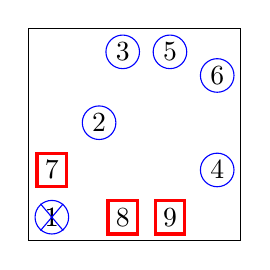
\begin{tikzpicture}[x = 3mm, y=3mm]
	\draw (-1,-1) rectangle (8,8);
	\tikzstyle{Square} = [
		draw = red, 
		very thick,
		rectangle,
		inner sep = 1mm,
		minimum size = 3 mm
	]
	\tikzstyle{SquareFill} = [
		draw = red, 
		fill = red,
		very thick,
		rectangle,
	]
	\tikzstyle{Circle} = [
		draw = blue, 
		circle,
		inner sep = 0.5 mm
	]
	\tikzstyle{CircleFill} = [
		draw = blue,
		fill = blue, 
		circle,
	]
	\node [Circle] (1) at (0,0) {1};
	\node [Circle] (2) at (2,4) {2};
	\node [Circle] (3) at (3,7) {3};
	\node [Circle] (4) at (7,2) {4};
	\node [Circle] (5) at (5,7) {5};
	\node [Circle] (6) at (7,6) {6};
	\node [Square] (7) at (0,2) {7};
	\node [Square] (8) at (3,0) {8};
	\node [Square] (9) at (5,0) {9};

	\node [Circle, cross out] (1) at (0,0) {1};
\end{tikzpicture}
\end{center}



Our original dataset has 619,027 samples.  We first removed the 27,723 crashes involving a pedestrian, leaving 591,304 samples.  Each sample had 82 features; we cut the number of features to 38 for our ``Hard'' features, then to 21 for ``Medium,'' and to 10 for ``Easy.''  We then split each of those three datasets 70/30 into a training set of 413,913 samples and a test set of 177,393 samples, preserving the proportions of negative and positive samples in both sets.  We did the train/test split twice with different random seeds (``Round 1'' and ``Round 2'') to gauge how much of the small differences in results were due to stochasticity instead of differences in the model algorithms or hyperparameters.  Tomek undersampling only applies to the training set, not to the test set.  

We then ran Imbalanced-Learn's  TomekLinks algorithm, then ran it again on the results to give our ``Tomek Once'' and ``Tomek Twice'' undersampled datasets.  

\

\hfil\begin{tabular}{lrrl}
\multicolumn{2}{l}{Hard Features, Round 1}   &  & \cr
 & Samples & \multicolumn{2}{c}{Change} \cr\hline
Original & 413,913 &  & \cr
Tomek Once & 399,515 & 14,398 & 3.48\%\cr
Tomek Twice & 396,511 & 3,004 & 0.75\%\cr\cline{3-4}
Total Change &  & 17,402 & 4.23\%\cr
\end{tabular}
\qquad\begin{tabular}{lrrl}
\multicolumn{2}{l}{Hard Features, Round 2} & \cr
 & Samples & \multicolumn{2}{c}{Change} \cr\hline
Original & 413,913 &  & \cr
Tomek Once & 399,714 & 14,199 & 3.43\%\cr
Tomek Twice & 396,718 & 2,996 & 0.75\%\cr\cline{3-4}
Total Change &  & 17,195 & 4.18\%\cr
\end{tabular}

\vskip 12pt

\hfil\begin{tabular}{lrrl}
\multicolumn{3}{l}{Medium Features, Round 1} & \cr
 & Samples & \multicolumn{2}{c}{Change} \cr\hline
Original & 413,913 &  & \cr
Tomek Once & 406,691 & 7,222 & 1.74\%\cr
Tomek Twice & 405,288 & 1,403 & 0.34\%\cr\cline{3-4}
Total Change &  & 8,625 & 2.08\%\cr
\end{tabular}
\qquad
\begin{tabular}{lrrl}
\multicolumn{3}{l}{Medium Features, Round 2} & \cr
 & Samples & \multicolumn{2}{c}{Change} \cr\hline
Original & 413,913 &  & \cr
Tomek Once & 406,781 & 7,132 & 1.72\%\cr
Tomek Twice & 405,368 & 1,413 & 0.35\%\cr\cline{3-4}
Total Change &  & 8,545 & 2.07\%\cr
\end{tabular}

\vskip 12pt

\hfil\begin{tabular}{lrrl}
\multicolumn{2}{l}{Easy Features, Round 1} & \cr
 & Samples & \multicolumn{2}{c}{Change} \cr\hline
Original & 413,913 &  & \cr
Tomek Once & 413,909 & 4 & 0.00097\%\cr
Tomek Twice & 413,908 & 1 & 0.00024\%\cr\cline{3-4}
Total Change &  & 5 & 0.00121\%\cr
\end{tabular}
\qquad
\begin{tabular}{lrrl}
\multicolumn{2}{l}{Easy Features, Round 2} & \cr
 & Samples & \multicolumn{2}{c}{Change} \cr\hline
Original & 413,913 &  & \cr
Tomek Once & 413,908 & 5 & 0.00121\%\cr
Tomek Twice & 413,907 & 1 & 0.00024\%\cr\cline{3-4}
Total Change &  & 6 & 0.00145\%\cr
\end{tabular}

\

We ran the models on the two rounds of Tomek undersampled training for the Hard-feature and Medium-feature sets, not for the Easy because the undersampling was so small.  

We were disappointed to not see a significant improvement in the model metrics from the undersampling; the difference between no undersampling, one runs of Tomek, and two runs turned out to be inconsequential, by which we mean that one approach was not consistently better when we ran the models with different random seeds.  


\subsubsection{Modifying the Loss Function}

A popular and well established way to modify the loss function for imbalanced data is with class weights, which can have the same effect as na{\"i}ve oversampling.  

Three of our seven models take class weights, and for those we tried three different class weights.  The Tomek undersampling changes the last weight slightly from $0.8499$ to as low as $0.8433$.

\

\hfil\begin{tabular}{c|l}
	$\alpha$ & Meaning \cr\hline
	1/2 & No class weight \cr
	2/3 & $\Delta FP/\Delta TP < 2.0$ goal \cr
	$0.85$ & Balanced classes \cr 
\end{tabular}

\


A related method is with focal loss, which has a modulating hyperparameter $\gamma$ that increases the penalty for low-confidence samples. \citep{lin2017focal}  We tried five values  of $\gamma$.

\

\hfil\begin{tabular}{c|c}
	$\gamma$  & Notes \cr\hline
	0.0 & Same as binary crossentropy \cr
	0.5 & Very light modulation \cr
	1.0 & Light modulation\cr
	2.0 & Recommended by Lin \cr
	5.0 & Heavy modulation \cr
\end{tabular}	

\

We did not see significant improvement using focal loss.  ({\bf Put in Label Reference}).

%%%
\subsubsection{Metrics for Imbalance}

In the \nameref{Methods_Metrics} subsection above we defined the metrics recall, precision, and f1.  The most common metric in machine learning, the one that most algorithms are designed to maximize, is accuracy, the proportion of samples correctly classified.  In that section's example of transformed model output, we had 150,107 out of 177,392 test samples correctly classified, giving 84.6\% accuracy.  Is that good?  The model below, the raw results of the Logistic Regression model of the easy features set, recommends sending no ambulances, and it is correct in 150,771 of 177,392 test samples, giving 84.99\% accuracy.  Is that better?



\

%%%
\parbox{\linewidth}{
%{\bf Balanced Random Forest model, Hard features, No Tomek, $\alpha = 2/3$}

\noindent\begin{tabular}{@{\hspace{-6pt}}p{2.3in} @{\hspace{-6pt}}p{2.0in} p{1.8in}}
	\vskip 0pt
	\qquad \qquad Raw Model Output
	
	\input{../Keras/Images/LRC_Easy_Tomek_0_alpha_0_5_v1_Pred.pgf}
&
	\vskip 0pt
	\qquad \qquad ROC Curve
	
	\input{../Keras/Images/LRC_Easy_Tomek_0_alpha_0_5_v1_ROC.pgf}
	
&
	\vskip 0pt
	\begin{tabular}{cc|c|c|}
	&\multicolumn{1}{c}{}& \multicolumn{2}{c}{Prediction} \cr
	&\multicolumn{1}{c}{} & \multicolumn{1}{c}{N} & \multicolumn{1}{c}{P} \cr\cline{3-4}
	\multirow{2}{*}{\rotatebox[origin=c]{90}{Actual}}&N &
150,771 & 0
	\vrule width 0pt height 10pt depth 2pt \cr\cline{3-4}
	&P & 
26621 & 0
	\vrule width 0pt height 10pt depth 2pt \cr\cline{3-4}
	\end{tabular}

	\hfil\begin{tabular}{ll}
	\cr
	0.8499 & Accuracy\cr
und & Precision \cr	0.0 & Recall \cr	und & F1 \cr	0.659 & AUC \cr
\end{tabular}

\cr
\end{tabular}
} % End parbox

\

In this study, we  have arbitrarily decided that we are willing to trade off up to two false positives to get one more true positive.  Once we moved our decision thresholds to the ethical tradeoff point, the accuracy only varied from 0.836 to 0.854.  The difference in accuracy tells us how many more (or fewer) false positives than true positives we have, with them being equal at 0.8499, and we get the same information from precision being less than, more than, or equal to 0.5.    Therefore, we are not going to consider accuracy in evaluating our models. 

%%%
\subsubsection{ML Algorithms for Imbalanced Data}

{\bf [Expand this subsubsection]}

\begin{itemize}
	\item Random Undersampling Composite Models
	\item Bagging
	\item Boosting
\end{itemize}

%%%%%
\subsection{Models}

We used seven binary classification algorithms.  Three of them take class weights.

\

\hfil\begin{tabular}{llc}
&& Class \cr
Model & Source & Weights \cr\hline
KerasClassifier with the Binary Focal Crossentropy loss function & Keras & Yes \cr
Balanced Random Forest Classifier & Imbalanced-Learn & Yes \cr
Balanced Bagging Classifier & Imbalanced-Learn & No \cr
RUSBoost Classifier & Imbalanced-Learn & No \cr
Easy Ensemble Classifier with AdaBoost Estimator & Imbalanced-Learn & No \cr
Logistic Regression Classifier & Scikit-Learn & Yes \cr
AdaBoost  Classifier & Scikit-Learn & No \cr
\end{tabular}

\


For the focal loss function, we tried seven different combinations of the hyperparameters $\alpha$ for class weights and $\gamma$ for penalty on badly misclassified samples.  For the random forest and bagging models we tried three values of $\alpha$.  Altogether we had seventeen model/hyperparameter combinations.  We learned each of the seven models on datasets with the easy, medium, and hard features, and on the hard features we tested with Tomek undersampling 0, 1, and 2 times, for a total of five datasets, giving eighty-five model/hyperparameter/dataset combinations.    We learned each of those sixty-five with two different random seeds, for a total of one hundred seventy results.  

\

\hfil\noindent\begin{tabular}{ccc}
	\multicolumn{3}{c}{Seventeen Models} \cr
	Model & $\alpha$ & $\gamma$ \cr\hline
	Focal & 1/2 & 0.0 \cr
	Focal & 2/3 & 0.0 \cr
	Focal & 2/3 & 0.5 \cr
	Focal & 2/3 & 1.0 \cr
	Focal & 2/3 & 2.0 \cr
	Focal & 2/3 & 5.0 \cr
	Focal & 0.85 & 0.0 \cr
	Random Forest & 1/2 & \cr
	Random Forest & 2/3 & \cr
	Random Forest & 0.85 & \cr
	Bagging && \cr
	RUSBoost && \cr
	Easy Ens && \cr
	Log Reg & 1/2 & \cr
	Log Reg & 2/3 & \cr
	Log Reg & 0.85 & \cr
	AdaBoost && \cr
\end{tabular}
\quad
$\times$
\quad
\begin{tabular}{cc}
	\multicolumn{2}{c}{Seven Datasets} \cr
	Features & Tomek \cr\hline
	Hard & None \cr
	Hard & Once \cr
	Hard & Twice \cr
	Medium & None \cr
	Medium & Once \cr
	Medium & Twice \cr
	Easy & None \cr
\end{tabular}
\quad
$\times$
\quad
\begin{tabular}{cc}
	Run twice with \cr
	different \cr
	random seeds \cr\hline
	Random seed 1 \cr
	Random seed 2
\end{tabular}
\quad 
$=$ 
\quad 
\begin{tabular}{c}
	238  \cr Sets of  \cr
	Results \cr
\end{tabular}









\subsection{Analysis of Results}\label{Analysis}
% Analysis of Results

Our ML algorithms assign to each sample (feature vector, crash person) a probability $p \in [0,1]$ that the person needs an ambulance.  The histogram below left shows the percentage of the dataset in each range of $p$, showing the percentages for the negative class (``Does not need an ambulance'') and the positive class (``Needs an ambulance'').  On the right, the Receiver Operating Characteristic (ROC) curve, and particularly the area under the curve (AUC), is a metric for how well the model separates the two classes, with $AUC=1.0$ being perfect and $AUC=0.5$ (the dashed line) being just random assignment with no insight.  

We would love to have results like in the graphs below, where the machine learning (ML) algorithm nearly perfectly separates the two classes.  There is some overlap between $p=0.6$ and $p=0.8$ with some samples the algorithm misclassifies, but the model clearly separates most samples.  Having an AUC of 0.996 would be amazing.  

\noindent\begin{tabular}{@{\hspace{-6pt}}p{4.3in} @{\hspace{-6pt}}p{2.0in}}
	\vskip 0pt
	\hfil Raw Model Output
	
	%% Creator: Matplotlib, PGF backend
%%
%% To include the figure in your LaTeX document, write
%%   \input{<filename>.pgf}
%%
%% Make sure the required packages are loaded in your preamble
%%   \usepackage{pgf}
%%
%% Also ensure that all the required font packages are loaded; for instance,
%% the lmodern package is sometimes necessary when using math font.
%%   \usepackage{lmodern}
%%
%% Figures using additional raster images can only be included by \input if
%% they are in the same directory as the main LaTeX file. For loading figures
%% from other directories you can use the `import` package
%%   \usepackage{import}
%%
%% and then include the figures with
%%   \import{<path to file>}{<filename>.pgf}
%%
%% Matplotlib used the following preamble
%%   
%%   \usepackage{fontspec}
%%   \makeatletter\@ifpackageloaded{underscore}{}{\usepackage[strings]{underscore}}\makeatother
%%
\begingroup%
\makeatletter%
\begin{pgfpicture}%
\pgfpathrectangle{\pgfpointorigin}{\pgfqpoint{4.509306in}{1.754444in}}%
\pgfusepath{use as bounding box, clip}%
\begin{pgfscope}%
\pgfsetbuttcap%
\pgfsetmiterjoin%
\definecolor{currentfill}{rgb}{1.000000,1.000000,1.000000}%
\pgfsetfillcolor{currentfill}%
\pgfsetlinewidth{0.000000pt}%
\definecolor{currentstroke}{rgb}{1.000000,1.000000,1.000000}%
\pgfsetstrokecolor{currentstroke}%
\pgfsetdash{}{0pt}%
\pgfpathmoveto{\pgfqpoint{0.000000in}{0.000000in}}%
\pgfpathlineto{\pgfqpoint{4.509306in}{0.000000in}}%
\pgfpathlineto{\pgfqpoint{4.509306in}{1.754444in}}%
\pgfpathlineto{\pgfqpoint{0.000000in}{1.754444in}}%
\pgfpathlineto{\pgfqpoint{0.000000in}{0.000000in}}%
\pgfpathclose%
\pgfusepath{fill}%
\end{pgfscope}%
\begin{pgfscope}%
\pgfsetbuttcap%
\pgfsetmiterjoin%
\definecolor{currentfill}{rgb}{1.000000,1.000000,1.000000}%
\pgfsetfillcolor{currentfill}%
\pgfsetlinewidth{0.000000pt}%
\definecolor{currentstroke}{rgb}{0.000000,0.000000,0.000000}%
\pgfsetstrokecolor{currentstroke}%
\pgfsetstrokeopacity{0.000000}%
\pgfsetdash{}{0pt}%
\pgfpathmoveto{\pgfqpoint{0.445556in}{0.499444in}}%
\pgfpathlineto{\pgfqpoint{4.320556in}{0.499444in}}%
\pgfpathlineto{\pgfqpoint{4.320556in}{1.654444in}}%
\pgfpathlineto{\pgfqpoint{0.445556in}{1.654444in}}%
\pgfpathlineto{\pgfqpoint{0.445556in}{0.499444in}}%
\pgfpathclose%
\pgfusepath{fill}%
\end{pgfscope}%
\begin{pgfscope}%
\pgfpathrectangle{\pgfqpoint{0.445556in}{0.499444in}}{\pgfqpoint{3.875000in}{1.155000in}}%
\pgfusepath{clip}%
\pgfsetbuttcap%
\pgfsetmiterjoin%
\pgfsetlinewidth{1.003750pt}%
\definecolor{currentstroke}{rgb}{0.000000,0.000000,0.000000}%
\pgfsetstrokecolor{currentstroke}%
\pgfsetdash{}{0pt}%
\pgfpathmoveto{\pgfqpoint{0.435556in}{0.499444in}}%
\pgfpathlineto{\pgfqpoint{0.483922in}{0.499444in}}%
\pgfpathlineto{\pgfqpoint{0.483922in}{0.632510in}}%
\pgfpathlineto{\pgfqpoint{0.435556in}{0.632510in}}%
\pgfusepath{stroke}%
\end{pgfscope}%
\begin{pgfscope}%
\pgfpathrectangle{\pgfqpoint{0.445556in}{0.499444in}}{\pgfqpoint{3.875000in}{1.155000in}}%
\pgfusepath{clip}%
\pgfsetbuttcap%
\pgfsetmiterjoin%
\pgfsetlinewidth{1.003750pt}%
\definecolor{currentstroke}{rgb}{0.000000,0.000000,0.000000}%
\pgfsetstrokecolor{currentstroke}%
\pgfsetdash{}{0pt}%
\pgfpathmoveto{\pgfqpoint{0.576001in}{0.499444in}}%
\pgfpathlineto{\pgfqpoint{0.637387in}{0.499444in}}%
\pgfpathlineto{\pgfqpoint{0.637387in}{0.855505in}}%
\pgfpathlineto{\pgfqpoint{0.576001in}{0.855505in}}%
\pgfpathlineto{\pgfqpoint{0.576001in}{0.499444in}}%
\pgfpathclose%
\pgfusepath{stroke}%
\end{pgfscope}%
\begin{pgfscope}%
\pgfpathrectangle{\pgfqpoint{0.445556in}{0.499444in}}{\pgfqpoint{3.875000in}{1.155000in}}%
\pgfusepath{clip}%
\pgfsetbuttcap%
\pgfsetmiterjoin%
\pgfsetlinewidth{1.003750pt}%
\definecolor{currentstroke}{rgb}{0.000000,0.000000,0.000000}%
\pgfsetstrokecolor{currentstroke}%
\pgfsetdash{}{0pt}%
\pgfpathmoveto{\pgfqpoint{0.729467in}{0.499444in}}%
\pgfpathlineto{\pgfqpoint{0.790853in}{0.499444in}}%
\pgfpathlineto{\pgfqpoint{0.790853in}{1.087595in}}%
\pgfpathlineto{\pgfqpoint{0.729467in}{1.087595in}}%
\pgfpathlineto{\pgfqpoint{0.729467in}{0.499444in}}%
\pgfpathclose%
\pgfusepath{stroke}%
\end{pgfscope}%
\begin{pgfscope}%
\pgfpathrectangle{\pgfqpoint{0.445556in}{0.499444in}}{\pgfqpoint{3.875000in}{1.155000in}}%
\pgfusepath{clip}%
\pgfsetbuttcap%
\pgfsetmiterjoin%
\pgfsetlinewidth{1.003750pt}%
\definecolor{currentstroke}{rgb}{0.000000,0.000000,0.000000}%
\pgfsetstrokecolor{currentstroke}%
\pgfsetdash{}{0pt}%
\pgfpathmoveto{\pgfqpoint{0.882932in}{0.499444in}}%
\pgfpathlineto{\pgfqpoint{0.944318in}{0.499444in}}%
\pgfpathlineto{\pgfqpoint{0.944318in}{1.269324in}}%
\pgfpathlineto{\pgfqpoint{0.882932in}{1.269324in}}%
\pgfpathlineto{\pgfqpoint{0.882932in}{0.499444in}}%
\pgfpathclose%
\pgfusepath{stroke}%
\end{pgfscope}%
\begin{pgfscope}%
\pgfpathrectangle{\pgfqpoint{0.445556in}{0.499444in}}{\pgfqpoint{3.875000in}{1.155000in}}%
\pgfusepath{clip}%
\pgfsetbuttcap%
\pgfsetmiterjoin%
\pgfsetlinewidth{1.003750pt}%
\definecolor{currentstroke}{rgb}{0.000000,0.000000,0.000000}%
\pgfsetstrokecolor{currentstroke}%
\pgfsetdash{}{0pt}%
\pgfpathmoveto{\pgfqpoint{1.036397in}{0.499444in}}%
\pgfpathlineto{\pgfqpoint{1.097783in}{0.499444in}}%
\pgfpathlineto{\pgfqpoint{1.097783in}{1.428301in}}%
\pgfpathlineto{\pgfqpoint{1.036397in}{1.428301in}}%
\pgfpathlineto{\pgfqpoint{1.036397in}{0.499444in}}%
\pgfpathclose%
\pgfusepath{stroke}%
\end{pgfscope}%
\begin{pgfscope}%
\pgfpathrectangle{\pgfqpoint{0.445556in}{0.499444in}}{\pgfqpoint{3.875000in}{1.155000in}}%
\pgfusepath{clip}%
\pgfsetbuttcap%
\pgfsetmiterjoin%
\pgfsetlinewidth{1.003750pt}%
\definecolor{currentstroke}{rgb}{0.000000,0.000000,0.000000}%
\pgfsetstrokecolor{currentstroke}%
\pgfsetdash{}{0pt}%
\pgfpathmoveto{\pgfqpoint{1.189863in}{0.499444in}}%
\pgfpathlineto{\pgfqpoint{1.251249in}{0.499444in}}%
\pgfpathlineto{\pgfqpoint{1.251249in}{1.521593in}}%
\pgfpathlineto{\pgfqpoint{1.189863in}{1.521593in}}%
\pgfpathlineto{\pgfqpoint{1.189863in}{0.499444in}}%
\pgfpathclose%
\pgfusepath{stroke}%
\end{pgfscope}%
\begin{pgfscope}%
\pgfpathrectangle{\pgfqpoint{0.445556in}{0.499444in}}{\pgfqpoint{3.875000in}{1.155000in}}%
\pgfusepath{clip}%
\pgfsetbuttcap%
\pgfsetmiterjoin%
\pgfsetlinewidth{1.003750pt}%
\definecolor{currentstroke}{rgb}{0.000000,0.000000,0.000000}%
\pgfsetstrokecolor{currentstroke}%
\pgfsetdash{}{0pt}%
\pgfpathmoveto{\pgfqpoint{1.343328in}{0.499444in}}%
\pgfpathlineto{\pgfqpoint{1.404714in}{0.499444in}}%
\pgfpathlineto{\pgfqpoint{1.404714in}{1.590875in}}%
\pgfpathlineto{\pgfqpoint{1.343328in}{1.590875in}}%
\pgfpathlineto{\pgfqpoint{1.343328in}{0.499444in}}%
\pgfpathclose%
\pgfusepath{stroke}%
\end{pgfscope}%
\begin{pgfscope}%
\pgfpathrectangle{\pgfqpoint{0.445556in}{0.499444in}}{\pgfqpoint{3.875000in}{1.155000in}}%
\pgfusepath{clip}%
\pgfsetbuttcap%
\pgfsetmiterjoin%
\pgfsetlinewidth{1.003750pt}%
\definecolor{currentstroke}{rgb}{0.000000,0.000000,0.000000}%
\pgfsetstrokecolor{currentstroke}%
\pgfsetdash{}{0pt}%
\pgfpathmoveto{\pgfqpoint{1.496793in}{0.499444in}}%
\pgfpathlineto{\pgfqpoint{1.558179in}{0.499444in}}%
\pgfpathlineto{\pgfqpoint{1.558179in}{1.599444in}}%
\pgfpathlineto{\pgfqpoint{1.496793in}{1.599444in}}%
\pgfpathlineto{\pgfqpoint{1.496793in}{0.499444in}}%
\pgfpathclose%
\pgfusepath{stroke}%
\end{pgfscope}%
\begin{pgfscope}%
\pgfpathrectangle{\pgfqpoint{0.445556in}{0.499444in}}{\pgfqpoint{3.875000in}{1.155000in}}%
\pgfusepath{clip}%
\pgfsetbuttcap%
\pgfsetmiterjoin%
\pgfsetlinewidth{1.003750pt}%
\definecolor{currentstroke}{rgb}{0.000000,0.000000,0.000000}%
\pgfsetstrokecolor{currentstroke}%
\pgfsetdash{}{0pt}%
\pgfpathmoveto{\pgfqpoint{1.650259in}{0.499444in}}%
\pgfpathlineto{\pgfqpoint{1.711645in}{0.499444in}}%
\pgfpathlineto{\pgfqpoint{1.711645in}{1.566953in}}%
\pgfpathlineto{\pgfqpoint{1.650259in}{1.566953in}}%
\pgfpathlineto{\pgfqpoint{1.650259in}{0.499444in}}%
\pgfpathclose%
\pgfusepath{stroke}%
\end{pgfscope}%
\begin{pgfscope}%
\pgfpathrectangle{\pgfqpoint{0.445556in}{0.499444in}}{\pgfqpoint{3.875000in}{1.155000in}}%
\pgfusepath{clip}%
\pgfsetbuttcap%
\pgfsetmiterjoin%
\pgfsetlinewidth{1.003750pt}%
\definecolor{currentstroke}{rgb}{0.000000,0.000000,0.000000}%
\pgfsetstrokecolor{currentstroke}%
\pgfsetdash{}{0pt}%
\pgfpathmoveto{\pgfqpoint{1.803724in}{0.499444in}}%
\pgfpathlineto{\pgfqpoint{1.865110in}{0.499444in}}%
\pgfpathlineto{\pgfqpoint{1.865110in}{1.506942in}}%
\pgfpathlineto{\pgfqpoint{1.803724in}{1.506942in}}%
\pgfpathlineto{\pgfqpoint{1.803724in}{0.499444in}}%
\pgfpathclose%
\pgfusepath{stroke}%
\end{pgfscope}%
\begin{pgfscope}%
\pgfpathrectangle{\pgfqpoint{0.445556in}{0.499444in}}{\pgfqpoint{3.875000in}{1.155000in}}%
\pgfusepath{clip}%
\pgfsetbuttcap%
\pgfsetmiterjoin%
\pgfsetlinewidth{1.003750pt}%
\definecolor{currentstroke}{rgb}{0.000000,0.000000,0.000000}%
\pgfsetstrokecolor{currentstroke}%
\pgfsetdash{}{0pt}%
\pgfpathmoveto{\pgfqpoint{1.957189in}{0.499444in}}%
\pgfpathlineto{\pgfqpoint{2.018575in}{0.499444in}}%
\pgfpathlineto{\pgfqpoint{2.018575in}{1.416545in}}%
\pgfpathlineto{\pgfqpoint{1.957189in}{1.416545in}}%
\pgfpathlineto{\pgfqpoint{1.957189in}{0.499444in}}%
\pgfpathclose%
\pgfusepath{stroke}%
\end{pgfscope}%
\begin{pgfscope}%
\pgfpathrectangle{\pgfqpoint{0.445556in}{0.499444in}}{\pgfqpoint{3.875000in}{1.155000in}}%
\pgfusepath{clip}%
\pgfsetbuttcap%
\pgfsetmiterjoin%
\pgfsetlinewidth{1.003750pt}%
\definecolor{currentstroke}{rgb}{0.000000,0.000000,0.000000}%
\pgfsetstrokecolor{currentstroke}%
\pgfsetdash{}{0pt}%
\pgfpathmoveto{\pgfqpoint{2.110655in}{0.499444in}}%
\pgfpathlineto{\pgfqpoint{2.172041in}{0.499444in}}%
\pgfpathlineto{\pgfqpoint{2.172041in}{1.298482in}}%
\pgfpathlineto{\pgfqpoint{2.110655in}{1.298482in}}%
\pgfpathlineto{\pgfqpoint{2.110655in}{0.499444in}}%
\pgfpathclose%
\pgfusepath{stroke}%
\end{pgfscope}%
\begin{pgfscope}%
\pgfpathrectangle{\pgfqpoint{0.445556in}{0.499444in}}{\pgfqpoint{3.875000in}{1.155000in}}%
\pgfusepath{clip}%
\pgfsetbuttcap%
\pgfsetmiterjoin%
\pgfsetlinewidth{1.003750pt}%
\definecolor{currentstroke}{rgb}{0.000000,0.000000,0.000000}%
\pgfsetstrokecolor{currentstroke}%
\pgfsetdash{}{0pt}%
\pgfpathmoveto{\pgfqpoint{2.264120in}{0.499444in}}%
\pgfpathlineto{\pgfqpoint{2.325506in}{0.499444in}}%
\pgfpathlineto{\pgfqpoint{2.325506in}{1.165884in}}%
\pgfpathlineto{\pgfqpoint{2.264120in}{1.165884in}}%
\pgfpathlineto{\pgfqpoint{2.264120in}{0.499444in}}%
\pgfpathclose%
\pgfusepath{stroke}%
\end{pgfscope}%
\begin{pgfscope}%
\pgfpathrectangle{\pgfqpoint{0.445556in}{0.499444in}}{\pgfqpoint{3.875000in}{1.155000in}}%
\pgfusepath{clip}%
\pgfsetbuttcap%
\pgfsetmiterjoin%
\pgfsetlinewidth{1.003750pt}%
\definecolor{currentstroke}{rgb}{0.000000,0.000000,0.000000}%
\pgfsetstrokecolor{currentstroke}%
\pgfsetdash{}{0pt}%
\pgfpathmoveto{\pgfqpoint{2.417585in}{0.499444in}}%
\pgfpathlineto{\pgfqpoint{2.478972in}{0.499444in}}%
\pgfpathlineto{\pgfqpoint{2.478972in}{1.041650in}}%
\pgfpathlineto{\pgfqpoint{2.417585in}{1.041650in}}%
\pgfpathlineto{\pgfqpoint{2.417585in}{0.499444in}}%
\pgfpathclose%
\pgfusepath{stroke}%
\end{pgfscope}%
\begin{pgfscope}%
\pgfpathrectangle{\pgfqpoint{0.445556in}{0.499444in}}{\pgfqpoint{3.875000in}{1.155000in}}%
\pgfusepath{clip}%
\pgfsetbuttcap%
\pgfsetmiterjoin%
\pgfsetlinewidth{1.003750pt}%
\definecolor{currentstroke}{rgb}{0.000000,0.000000,0.000000}%
\pgfsetstrokecolor{currentstroke}%
\pgfsetdash{}{0pt}%
\pgfpathmoveto{\pgfqpoint{2.571051in}{0.499444in}}%
\pgfpathlineto{\pgfqpoint{2.632437in}{0.499444in}}%
\pgfpathlineto{\pgfqpoint{2.632437in}{0.916218in}}%
\pgfpathlineto{\pgfqpoint{2.571051in}{0.916218in}}%
\pgfpathlineto{\pgfqpoint{2.571051in}{0.499444in}}%
\pgfpathclose%
\pgfusepath{stroke}%
\end{pgfscope}%
\begin{pgfscope}%
\pgfpathrectangle{\pgfqpoint{0.445556in}{0.499444in}}{\pgfqpoint{3.875000in}{1.155000in}}%
\pgfusepath{clip}%
\pgfsetbuttcap%
\pgfsetmiterjoin%
\pgfsetlinewidth{1.003750pt}%
\definecolor{currentstroke}{rgb}{0.000000,0.000000,0.000000}%
\pgfsetstrokecolor{currentstroke}%
\pgfsetdash{}{0pt}%
\pgfpathmoveto{\pgfqpoint{2.724516in}{0.499444in}}%
\pgfpathlineto{\pgfqpoint{2.785902in}{0.499444in}}%
\pgfpathlineto{\pgfqpoint{2.785902in}{0.806958in}}%
\pgfpathlineto{\pgfqpoint{2.724516in}{0.806958in}}%
\pgfpathlineto{\pgfqpoint{2.724516in}{0.499444in}}%
\pgfpathclose%
\pgfusepath{stroke}%
\end{pgfscope}%
\begin{pgfscope}%
\pgfpathrectangle{\pgfqpoint{0.445556in}{0.499444in}}{\pgfqpoint{3.875000in}{1.155000in}}%
\pgfusepath{clip}%
\pgfsetbuttcap%
\pgfsetmiterjoin%
\pgfsetlinewidth{1.003750pt}%
\definecolor{currentstroke}{rgb}{0.000000,0.000000,0.000000}%
\pgfsetstrokecolor{currentstroke}%
\pgfsetdash{}{0pt}%
\pgfpathmoveto{\pgfqpoint{2.877981in}{0.499444in}}%
\pgfpathlineto{\pgfqpoint{2.939368in}{0.499444in}}%
\pgfpathlineto{\pgfqpoint{2.939368in}{0.716063in}}%
\pgfpathlineto{\pgfqpoint{2.877981in}{0.716063in}}%
\pgfpathlineto{\pgfqpoint{2.877981in}{0.499444in}}%
\pgfpathclose%
\pgfusepath{stroke}%
\end{pgfscope}%
\begin{pgfscope}%
\pgfpathrectangle{\pgfqpoint{0.445556in}{0.499444in}}{\pgfqpoint{3.875000in}{1.155000in}}%
\pgfusepath{clip}%
\pgfsetbuttcap%
\pgfsetmiterjoin%
\pgfsetlinewidth{1.003750pt}%
\definecolor{currentstroke}{rgb}{0.000000,0.000000,0.000000}%
\pgfsetstrokecolor{currentstroke}%
\pgfsetdash{}{0pt}%
\pgfpathmoveto{\pgfqpoint{3.031447in}{0.499444in}}%
\pgfpathlineto{\pgfqpoint{3.092833in}{0.499444in}}%
\pgfpathlineto{\pgfqpoint{3.092833in}{0.645904in}}%
\pgfpathlineto{\pgfqpoint{3.031447in}{0.645904in}}%
\pgfpathlineto{\pgfqpoint{3.031447in}{0.499444in}}%
\pgfpathclose%
\pgfusepath{stroke}%
\end{pgfscope}%
\begin{pgfscope}%
\pgfpathrectangle{\pgfqpoint{0.445556in}{0.499444in}}{\pgfqpoint{3.875000in}{1.155000in}}%
\pgfusepath{clip}%
\pgfsetbuttcap%
\pgfsetmiterjoin%
\pgfsetlinewidth{1.003750pt}%
\definecolor{currentstroke}{rgb}{0.000000,0.000000,0.000000}%
\pgfsetstrokecolor{currentstroke}%
\pgfsetdash{}{0pt}%
\pgfpathmoveto{\pgfqpoint{3.184912in}{0.499444in}}%
\pgfpathlineto{\pgfqpoint{3.246298in}{0.499444in}}%
\pgfpathlineto{\pgfqpoint{3.246298in}{0.598936in}}%
\pgfpathlineto{\pgfqpoint{3.184912in}{0.598936in}}%
\pgfpathlineto{\pgfqpoint{3.184912in}{0.499444in}}%
\pgfpathclose%
\pgfusepath{stroke}%
\end{pgfscope}%
\begin{pgfscope}%
\pgfpathrectangle{\pgfqpoint{0.445556in}{0.499444in}}{\pgfqpoint{3.875000in}{1.155000in}}%
\pgfusepath{clip}%
\pgfsetbuttcap%
\pgfsetmiterjoin%
\pgfsetlinewidth{1.003750pt}%
\definecolor{currentstroke}{rgb}{0.000000,0.000000,0.000000}%
\pgfsetstrokecolor{currentstroke}%
\pgfsetdash{}{0pt}%
\pgfpathmoveto{\pgfqpoint{3.338377in}{0.499444in}}%
\pgfpathlineto{\pgfqpoint{3.399764in}{0.499444in}}%
\pgfpathlineto{\pgfqpoint{3.399764in}{0.560040in}}%
\pgfpathlineto{\pgfqpoint{3.338377in}{0.560040in}}%
\pgfpathlineto{\pgfqpoint{3.338377in}{0.499444in}}%
\pgfpathclose%
\pgfusepath{stroke}%
\end{pgfscope}%
\begin{pgfscope}%
\pgfpathrectangle{\pgfqpoint{0.445556in}{0.499444in}}{\pgfqpoint{3.875000in}{1.155000in}}%
\pgfusepath{clip}%
\pgfsetbuttcap%
\pgfsetmiterjoin%
\pgfsetlinewidth{1.003750pt}%
\definecolor{currentstroke}{rgb}{0.000000,0.000000,0.000000}%
\pgfsetstrokecolor{currentstroke}%
\pgfsetdash{}{0pt}%
\pgfpathmoveto{\pgfqpoint{3.491843in}{0.499444in}}%
\pgfpathlineto{\pgfqpoint{3.553229in}{0.499444in}}%
\pgfpathlineto{\pgfqpoint{3.553229in}{0.535591in}}%
\pgfpathlineto{\pgfqpoint{3.491843in}{0.535591in}}%
\pgfpathlineto{\pgfqpoint{3.491843in}{0.499444in}}%
\pgfpathclose%
\pgfusepath{stroke}%
\end{pgfscope}%
\begin{pgfscope}%
\pgfpathrectangle{\pgfqpoint{0.445556in}{0.499444in}}{\pgfqpoint{3.875000in}{1.155000in}}%
\pgfusepath{clip}%
\pgfsetbuttcap%
\pgfsetmiterjoin%
\pgfsetlinewidth{1.003750pt}%
\definecolor{currentstroke}{rgb}{0.000000,0.000000,0.000000}%
\pgfsetstrokecolor{currentstroke}%
\pgfsetdash{}{0pt}%
\pgfpathmoveto{\pgfqpoint{3.645308in}{0.499444in}}%
\pgfpathlineto{\pgfqpoint{3.706694in}{0.499444in}}%
\pgfpathlineto{\pgfqpoint{3.706694in}{0.512137in}}%
\pgfpathlineto{\pgfqpoint{3.645308in}{0.512137in}}%
\pgfpathlineto{\pgfqpoint{3.645308in}{0.499444in}}%
\pgfpathclose%
\pgfusepath{stroke}%
\end{pgfscope}%
\begin{pgfscope}%
\pgfpathrectangle{\pgfqpoint{0.445556in}{0.499444in}}{\pgfqpoint{3.875000in}{1.155000in}}%
\pgfusepath{clip}%
\pgfsetbuttcap%
\pgfsetmiterjoin%
\pgfsetlinewidth{1.003750pt}%
\definecolor{currentstroke}{rgb}{0.000000,0.000000,0.000000}%
\pgfsetstrokecolor{currentstroke}%
\pgfsetdash{}{0pt}%
\pgfpathmoveto{\pgfqpoint{3.798774in}{0.499444in}}%
\pgfpathlineto{\pgfqpoint{3.860160in}{0.499444in}}%
\pgfpathlineto{\pgfqpoint{3.860160in}{0.503305in}}%
\pgfpathlineto{\pgfqpoint{3.798774in}{0.503305in}}%
\pgfpathlineto{\pgfqpoint{3.798774in}{0.499444in}}%
\pgfpathclose%
\pgfusepath{stroke}%
\end{pgfscope}%
\begin{pgfscope}%
\pgfpathrectangle{\pgfqpoint{0.445556in}{0.499444in}}{\pgfqpoint{3.875000in}{1.155000in}}%
\pgfusepath{clip}%
\pgfsetbuttcap%
\pgfsetmiterjoin%
\pgfsetlinewidth{1.003750pt}%
\definecolor{currentstroke}{rgb}{0.000000,0.000000,0.000000}%
\pgfsetstrokecolor{currentstroke}%
\pgfsetdash{}{0pt}%
\pgfpathmoveto{\pgfqpoint{3.952239in}{0.499444in}}%
\pgfpathlineto{\pgfqpoint{4.013625in}{0.499444in}}%
\pgfpathlineto{\pgfqpoint{4.013625in}{0.500234in}}%
\pgfpathlineto{\pgfqpoint{3.952239in}{0.500234in}}%
\pgfpathlineto{\pgfqpoint{3.952239in}{0.499444in}}%
\pgfpathclose%
\pgfusepath{stroke}%
\end{pgfscope}%
\begin{pgfscope}%
\pgfpathrectangle{\pgfqpoint{0.445556in}{0.499444in}}{\pgfqpoint{3.875000in}{1.155000in}}%
\pgfusepath{clip}%
\pgfsetbuttcap%
\pgfsetmiterjoin%
\pgfsetlinewidth{1.003750pt}%
\definecolor{currentstroke}{rgb}{0.000000,0.000000,0.000000}%
\pgfsetstrokecolor{currentstroke}%
\pgfsetdash{}{0pt}%
\pgfpathmoveto{\pgfqpoint{4.105704in}{0.499444in}}%
\pgfpathlineto{\pgfqpoint{4.167090in}{0.499444in}}%
\pgfpathlineto{\pgfqpoint{4.167090in}{0.499503in}}%
\pgfpathlineto{\pgfqpoint{4.105704in}{0.499503in}}%
\pgfpathlineto{\pgfqpoint{4.105704in}{0.499444in}}%
\pgfpathclose%
\pgfusepath{stroke}%
\end{pgfscope}%
\begin{pgfscope}%
\pgfpathrectangle{\pgfqpoint{0.445556in}{0.499444in}}{\pgfqpoint{3.875000in}{1.155000in}}%
\pgfusepath{clip}%
\pgfsetbuttcap%
\pgfsetmiterjoin%
\definecolor{currentfill}{rgb}{0.000000,0.000000,0.000000}%
\pgfsetfillcolor{currentfill}%
\pgfsetlinewidth{0.000000pt}%
\definecolor{currentstroke}{rgb}{0.000000,0.000000,0.000000}%
\pgfsetstrokecolor{currentstroke}%
\pgfsetstrokeopacity{0.000000}%
\pgfsetdash{}{0pt}%
\pgfpathmoveto{\pgfqpoint{0.483922in}{0.499444in}}%
\pgfpathlineto{\pgfqpoint{0.545308in}{0.499444in}}%
\pgfpathlineto{\pgfqpoint{0.545308in}{0.499444in}}%
\pgfpathlineto{\pgfqpoint{0.483922in}{0.499444in}}%
\pgfpathlineto{\pgfqpoint{0.483922in}{0.499444in}}%
\pgfpathclose%
\pgfusepath{fill}%
\end{pgfscope}%
\begin{pgfscope}%
\pgfpathrectangle{\pgfqpoint{0.445556in}{0.499444in}}{\pgfqpoint{3.875000in}{1.155000in}}%
\pgfusepath{clip}%
\pgfsetbuttcap%
\pgfsetmiterjoin%
\definecolor{currentfill}{rgb}{0.000000,0.000000,0.000000}%
\pgfsetfillcolor{currentfill}%
\pgfsetlinewidth{0.000000pt}%
\definecolor{currentstroke}{rgb}{0.000000,0.000000,0.000000}%
\pgfsetstrokecolor{currentstroke}%
\pgfsetstrokeopacity{0.000000}%
\pgfsetdash{}{0pt}%
\pgfpathmoveto{\pgfqpoint{0.637387in}{0.499444in}}%
\pgfpathlineto{\pgfqpoint{0.698774in}{0.499444in}}%
\pgfpathlineto{\pgfqpoint{0.698774in}{0.499444in}}%
\pgfpathlineto{\pgfqpoint{0.637387in}{0.499444in}}%
\pgfpathlineto{\pgfqpoint{0.637387in}{0.499444in}}%
\pgfpathclose%
\pgfusepath{fill}%
\end{pgfscope}%
\begin{pgfscope}%
\pgfpathrectangle{\pgfqpoint{0.445556in}{0.499444in}}{\pgfqpoint{3.875000in}{1.155000in}}%
\pgfusepath{clip}%
\pgfsetbuttcap%
\pgfsetmiterjoin%
\definecolor{currentfill}{rgb}{0.000000,0.000000,0.000000}%
\pgfsetfillcolor{currentfill}%
\pgfsetlinewidth{0.000000pt}%
\definecolor{currentstroke}{rgb}{0.000000,0.000000,0.000000}%
\pgfsetstrokecolor{currentstroke}%
\pgfsetstrokeopacity{0.000000}%
\pgfsetdash{}{0pt}%
\pgfpathmoveto{\pgfqpoint{0.790853in}{0.499444in}}%
\pgfpathlineto{\pgfqpoint{0.852239in}{0.499444in}}%
\pgfpathlineto{\pgfqpoint{0.852239in}{0.499444in}}%
\pgfpathlineto{\pgfqpoint{0.790853in}{0.499444in}}%
\pgfpathlineto{\pgfqpoint{0.790853in}{0.499444in}}%
\pgfpathclose%
\pgfusepath{fill}%
\end{pgfscope}%
\begin{pgfscope}%
\pgfpathrectangle{\pgfqpoint{0.445556in}{0.499444in}}{\pgfqpoint{3.875000in}{1.155000in}}%
\pgfusepath{clip}%
\pgfsetbuttcap%
\pgfsetmiterjoin%
\definecolor{currentfill}{rgb}{0.000000,0.000000,0.000000}%
\pgfsetfillcolor{currentfill}%
\pgfsetlinewidth{0.000000pt}%
\definecolor{currentstroke}{rgb}{0.000000,0.000000,0.000000}%
\pgfsetstrokecolor{currentstroke}%
\pgfsetstrokeopacity{0.000000}%
\pgfsetdash{}{0pt}%
\pgfpathmoveto{\pgfqpoint{0.944318in}{0.499444in}}%
\pgfpathlineto{\pgfqpoint{1.005704in}{0.499444in}}%
\pgfpathlineto{\pgfqpoint{1.005704in}{0.499444in}}%
\pgfpathlineto{\pgfqpoint{0.944318in}{0.499444in}}%
\pgfpathlineto{\pgfqpoint{0.944318in}{0.499444in}}%
\pgfpathclose%
\pgfusepath{fill}%
\end{pgfscope}%
\begin{pgfscope}%
\pgfpathrectangle{\pgfqpoint{0.445556in}{0.499444in}}{\pgfqpoint{3.875000in}{1.155000in}}%
\pgfusepath{clip}%
\pgfsetbuttcap%
\pgfsetmiterjoin%
\definecolor{currentfill}{rgb}{0.000000,0.000000,0.000000}%
\pgfsetfillcolor{currentfill}%
\pgfsetlinewidth{0.000000pt}%
\definecolor{currentstroke}{rgb}{0.000000,0.000000,0.000000}%
\pgfsetstrokecolor{currentstroke}%
\pgfsetstrokeopacity{0.000000}%
\pgfsetdash{}{0pt}%
\pgfpathmoveto{\pgfqpoint{1.097783in}{0.499444in}}%
\pgfpathlineto{\pgfqpoint{1.159170in}{0.499444in}}%
\pgfpathlineto{\pgfqpoint{1.159170in}{0.499444in}}%
\pgfpathlineto{\pgfqpoint{1.097783in}{0.499444in}}%
\pgfpathlineto{\pgfqpoint{1.097783in}{0.499444in}}%
\pgfpathclose%
\pgfusepath{fill}%
\end{pgfscope}%
\begin{pgfscope}%
\pgfpathrectangle{\pgfqpoint{0.445556in}{0.499444in}}{\pgfqpoint{3.875000in}{1.155000in}}%
\pgfusepath{clip}%
\pgfsetbuttcap%
\pgfsetmiterjoin%
\definecolor{currentfill}{rgb}{0.000000,0.000000,0.000000}%
\pgfsetfillcolor{currentfill}%
\pgfsetlinewidth{0.000000pt}%
\definecolor{currentstroke}{rgb}{0.000000,0.000000,0.000000}%
\pgfsetstrokecolor{currentstroke}%
\pgfsetstrokeopacity{0.000000}%
\pgfsetdash{}{0pt}%
\pgfpathmoveto{\pgfqpoint{1.251249in}{0.499444in}}%
\pgfpathlineto{\pgfqpoint{1.312635in}{0.499444in}}%
\pgfpathlineto{\pgfqpoint{1.312635in}{0.499444in}}%
\pgfpathlineto{\pgfqpoint{1.251249in}{0.499444in}}%
\pgfpathlineto{\pgfqpoint{1.251249in}{0.499444in}}%
\pgfpathclose%
\pgfusepath{fill}%
\end{pgfscope}%
\begin{pgfscope}%
\pgfpathrectangle{\pgfqpoint{0.445556in}{0.499444in}}{\pgfqpoint{3.875000in}{1.155000in}}%
\pgfusepath{clip}%
\pgfsetbuttcap%
\pgfsetmiterjoin%
\definecolor{currentfill}{rgb}{0.000000,0.000000,0.000000}%
\pgfsetfillcolor{currentfill}%
\pgfsetlinewidth{0.000000pt}%
\definecolor{currentstroke}{rgb}{0.000000,0.000000,0.000000}%
\pgfsetstrokecolor{currentstroke}%
\pgfsetstrokeopacity{0.000000}%
\pgfsetdash{}{0pt}%
\pgfpathmoveto{\pgfqpoint{1.404714in}{0.499444in}}%
\pgfpathlineto{\pgfqpoint{1.466100in}{0.499444in}}%
\pgfpathlineto{\pgfqpoint{1.466100in}{0.499444in}}%
\pgfpathlineto{\pgfqpoint{1.404714in}{0.499444in}}%
\pgfpathlineto{\pgfqpoint{1.404714in}{0.499444in}}%
\pgfpathclose%
\pgfusepath{fill}%
\end{pgfscope}%
\begin{pgfscope}%
\pgfpathrectangle{\pgfqpoint{0.445556in}{0.499444in}}{\pgfqpoint{3.875000in}{1.155000in}}%
\pgfusepath{clip}%
\pgfsetbuttcap%
\pgfsetmiterjoin%
\definecolor{currentfill}{rgb}{0.000000,0.000000,0.000000}%
\pgfsetfillcolor{currentfill}%
\pgfsetlinewidth{0.000000pt}%
\definecolor{currentstroke}{rgb}{0.000000,0.000000,0.000000}%
\pgfsetstrokecolor{currentstroke}%
\pgfsetstrokeopacity{0.000000}%
\pgfsetdash{}{0pt}%
\pgfpathmoveto{\pgfqpoint{1.558179in}{0.499444in}}%
\pgfpathlineto{\pgfqpoint{1.619566in}{0.499444in}}%
\pgfpathlineto{\pgfqpoint{1.619566in}{0.499444in}}%
\pgfpathlineto{\pgfqpoint{1.558179in}{0.499444in}}%
\pgfpathlineto{\pgfqpoint{1.558179in}{0.499444in}}%
\pgfpathclose%
\pgfusepath{fill}%
\end{pgfscope}%
\begin{pgfscope}%
\pgfpathrectangle{\pgfqpoint{0.445556in}{0.499444in}}{\pgfqpoint{3.875000in}{1.155000in}}%
\pgfusepath{clip}%
\pgfsetbuttcap%
\pgfsetmiterjoin%
\definecolor{currentfill}{rgb}{0.000000,0.000000,0.000000}%
\pgfsetfillcolor{currentfill}%
\pgfsetlinewidth{0.000000pt}%
\definecolor{currentstroke}{rgb}{0.000000,0.000000,0.000000}%
\pgfsetstrokecolor{currentstroke}%
\pgfsetstrokeopacity{0.000000}%
\pgfsetdash{}{0pt}%
\pgfpathmoveto{\pgfqpoint{1.711645in}{0.499444in}}%
\pgfpathlineto{\pgfqpoint{1.773031in}{0.499444in}}%
\pgfpathlineto{\pgfqpoint{1.773031in}{0.499444in}}%
\pgfpathlineto{\pgfqpoint{1.711645in}{0.499444in}}%
\pgfpathlineto{\pgfqpoint{1.711645in}{0.499444in}}%
\pgfpathclose%
\pgfusepath{fill}%
\end{pgfscope}%
\begin{pgfscope}%
\pgfpathrectangle{\pgfqpoint{0.445556in}{0.499444in}}{\pgfqpoint{3.875000in}{1.155000in}}%
\pgfusepath{clip}%
\pgfsetbuttcap%
\pgfsetmiterjoin%
\definecolor{currentfill}{rgb}{0.000000,0.000000,0.000000}%
\pgfsetfillcolor{currentfill}%
\pgfsetlinewidth{0.000000pt}%
\definecolor{currentstroke}{rgb}{0.000000,0.000000,0.000000}%
\pgfsetstrokecolor{currentstroke}%
\pgfsetstrokeopacity{0.000000}%
\pgfsetdash{}{0pt}%
\pgfpathmoveto{\pgfqpoint{1.865110in}{0.499444in}}%
\pgfpathlineto{\pgfqpoint{1.926496in}{0.499444in}}%
\pgfpathlineto{\pgfqpoint{1.926496in}{0.499444in}}%
\pgfpathlineto{\pgfqpoint{1.865110in}{0.499444in}}%
\pgfpathlineto{\pgfqpoint{1.865110in}{0.499444in}}%
\pgfpathclose%
\pgfusepath{fill}%
\end{pgfscope}%
\begin{pgfscope}%
\pgfpathrectangle{\pgfqpoint{0.445556in}{0.499444in}}{\pgfqpoint{3.875000in}{1.155000in}}%
\pgfusepath{clip}%
\pgfsetbuttcap%
\pgfsetmiterjoin%
\definecolor{currentfill}{rgb}{0.000000,0.000000,0.000000}%
\pgfsetfillcolor{currentfill}%
\pgfsetlinewidth{0.000000pt}%
\definecolor{currentstroke}{rgb}{0.000000,0.000000,0.000000}%
\pgfsetstrokecolor{currentstroke}%
\pgfsetstrokeopacity{0.000000}%
\pgfsetdash{}{0pt}%
\pgfpathmoveto{\pgfqpoint{2.018575in}{0.499444in}}%
\pgfpathlineto{\pgfqpoint{2.079962in}{0.499444in}}%
\pgfpathlineto{\pgfqpoint{2.079962in}{0.499444in}}%
\pgfpathlineto{\pgfqpoint{2.018575in}{0.499444in}}%
\pgfpathlineto{\pgfqpoint{2.018575in}{0.499444in}}%
\pgfpathclose%
\pgfusepath{fill}%
\end{pgfscope}%
\begin{pgfscope}%
\pgfpathrectangle{\pgfqpoint{0.445556in}{0.499444in}}{\pgfqpoint{3.875000in}{1.155000in}}%
\pgfusepath{clip}%
\pgfsetbuttcap%
\pgfsetmiterjoin%
\definecolor{currentfill}{rgb}{0.000000,0.000000,0.000000}%
\pgfsetfillcolor{currentfill}%
\pgfsetlinewidth{0.000000pt}%
\definecolor{currentstroke}{rgb}{0.000000,0.000000,0.000000}%
\pgfsetstrokecolor{currentstroke}%
\pgfsetstrokeopacity{0.000000}%
\pgfsetdash{}{0pt}%
\pgfpathmoveto{\pgfqpoint{2.172041in}{0.499444in}}%
\pgfpathlineto{\pgfqpoint{2.233427in}{0.499444in}}%
\pgfpathlineto{\pgfqpoint{2.233427in}{0.499444in}}%
\pgfpathlineto{\pgfqpoint{2.172041in}{0.499444in}}%
\pgfpathlineto{\pgfqpoint{2.172041in}{0.499444in}}%
\pgfpathclose%
\pgfusepath{fill}%
\end{pgfscope}%
\begin{pgfscope}%
\pgfpathrectangle{\pgfqpoint{0.445556in}{0.499444in}}{\pgfqpoint{3.875000in}{1.155000in}}%
\pgfusepath{clip}%
\pgfsetbuttcap%
\pgfsetmiterjoin%
\definecolor{currentfill}{rgb}{0.000000,0.000000,0.000000}%
\pgfsetfillcolor{currentfill}%
\pgfsetlinewidth{0.000000pt}%
\definecolor{currentstroke}{rgb}{0.000000,0.000000,0.000000}%
\pgfsetstrokecolor{currentstroke}%
\pgfsetstrokeopacity{0.000000}%
\pgfsetdash{}{0pt}%
\pgfpathmoveto{\pgfqpoint{2.325506in}{0.499444in}}%
\pgfpathlineto{\pgfqpoint{2.386892in}{0.499444in}}%
\pgfpathlineto{\pgfqpoint{2.386892in}{0.499561in}}%
\pgfpathlineto{\pgfqpoint{2.325506in}{0.499561in}}%
\pgfpathlineto{\pgfqpoint{2.325506in}{0.499444in}}%
\pgfpathclose%
\pgfusepath{fill}%
\end{pgfscope}%
\begin{pgfscope}%
\pgfpathrectangle{\pgfqpoint{0.445556in}{0.499444in}}{\pgfqpoint{3.875000in}{1.155000in}}%
\pgfusepath{clip}%
\pgfsetbuttcap%
\pgfsetmiterjoin%
\definecolor{currentfill}{rgb}{0.000000,0.000000,0.000000}%
\pgfsetfillcolor{currentfill}%
\pgfsetlinewidth{0.000000pt}%
\definecolor{currentstroke}{rgb}{0.000000,0.000000,0.000000}%
\pgfsetstrokecolor{currentstroke}%
\pgfsetstrokeopacity{0.000000}%
\pgfsetdash{}{0pt}%
\pgfpathmoveto{\pgfqpoint{2.478972in}{0.499444in}}%
\pgfpathlineto{\pgfqpoint{2.540358in}{0.499444in}}%
\pgfpathlineto{\pgfqpoint{2.540358in}{0.499854in}}%
\pgfpathlineto{\pgfqpoint{2.478972in}{0.499854in}}%
\pgfpathlineto{\pgfqpoint{2.478972in}{0.499444in}}%
\pgfpathclose%
\pgfusepath{fill}%
\end{pgfscope}%
\begin{pgfscope}%
\pgfpathrectangle{\pgfqpoint{0.445556in}{0.499444in}}{\pgfqpoint{3.875000in}{1.155000in}}%
\pgfusepath{clip}%
\pgfsetbuttcap%
\pgfsetmiterjoin%
\definecolor{currentfill}{rgb}{0.000000,0.000000,0.000000}%
\pgfsetfillcolor{currentfill}%
\pgfsetlinewidth{0.000000pt}%
\definecolor{currentstroke}{rgb}{0.000000,0.000000,0.000000}%
\pgfsetstrokecolor{currentstroke}%
\pgfsetstrokeopacity{0.000000}%
\pgfsetdash{}{0pt}%
\pgfpathmoveto{\pgfqpoint{2.632437in}{0.499444in}}%
\pgfpathlineto{\pgfqpoint{2.693823in}{0.499444in}}%
\pgfpathlineto{\pgfqpoint{2.693823in}{0.501521in}}%
\pgfpathlineto{\pgfqpoint{2.632437in}{0.501521in}}%
\pgfpathlineto{\pgfqpoint{2.632437in}{0.499444in}}%
\pgfpathclose%
\pgfusepath{fill}%
\end{pgfscope}%
\begin{pgfscope}%
\pgfpathrectangle{\pgfqpoint{0.445556in}{0.499444in}}{\pgfqpoint{3.875000in}{1.155000in}}%
\pgfusepath{clip}%
\pgfsetbuttcap%
\pgfsetmiterjoin%
\definecolor{currentfill}{rgb}{0.000000,0.000000,0.000000}%
\pgfsetfillcolor{currentfill}%
\pgfsetlinewidth{0.000000pt}%
\definecolor{currentstroke}{rgb}{0.000000,0.000000,0.000000}%
\pgfsetstrokecolor{currentstroke}%
\pgfsetstrokeopacity{0.000000}%
\pgfsetdash{}{0pt}%
\pgfpathmoveto{\pgfqpoint{2.785902in}{0.499444in}}%
\pgfpathlineto{\pgfqpoint{2.847288in}{0.499444in}}%
\pgfpathlineto{\pgfqpoint{2.847288in}{0.511171in}}%
\pgfpathlineto{\pgfqpoint{2.785902in}{0.511171in}}%
\pgfpathlineto{\pgfqpoint{2.785902in}{0.499444in}}%
\pgfpathclose%
\pgfusepath{fill}%
\end{pgfscope}%
\begin{pgfscope}%
\pgfpathrectangle{\pgfqpoint{0.445556in}{0.499444in}}{\pgfqpoint{3.875000in}{1.155000in}}%
\pgfusepath{clip}%
\pgfsetbuttcap%
\pgfsetmiterjoin%
\definecolor{currentfill}{rgb}{0.000000,0.000000,0.000000}%
\pgfsetfillcolor{currentfill}%
\pgfsetlinewidth{0.000000pt}%
\definecolor{currentstroke}{rgb}{0.000000,0.000000,0.000000}%
\pgfsetstrokecolor{currentstroke}%
\pgfsetstrokeopacity{0.000000}%
\pgfsetdash{}{0pt}%
\pgfpathmoveto{\pgfqpoint{2.939368in}{0.499444in}}%
\pgfpathlineto{\pgfqpoint{3.000754in}{0.499444in}}%
\pgfpathlineto{\pgfqpoint{3.000754in}{0.534889in}}%
\pgfpathlineto{\pgfqpoint{2.939368in}{0.534889in}}%
\pgfpathlineto{\pgfqpoint{2.939368in}{0.499444in}}%
\pgfpathclose%
\pgfusepath{fill}%
\end{pgfscope}%
\begin{pgfscope}%
\pgfpathrectangle{\pgfqpoint{0.445556in}{0.499444in}}{\pgfqpoint{3.875000in}{1.155000in}}%
\pgfusepath{clip}%
\pgfsetbuttcap%
\pgfsetmiterjoin%
\definecolor{currentfill}{rgb}{0.000000,0.000000,0.000000}%
\pgfsetfillcolor{currentfill}%
\pgfsetlinewidth{0.000000pt}%
\definecolor{currentstroke}{rgb}{0.000000,0.000000,0.000000}%
\pgfsetstrokecolor{currentstroke}%
\pgfsetstrokeopacity{0.000000}%
\pgfsetdash{}{0pt}%
\pgfpathmoveto{\pgfqpoint{3.092833in}{0.499444in}}%
\pgfpathlineto{\pgfqpoint{3.154219in}{0.499444in}}%
\pgfpathlineto{\pgfqpoint{3.154219in}{0.582998in}}%
\pgfpathlineto{\pgfqpoint{3.092833in}{0.582998in}}%
\pgfpathlineto{\pgfqpoint{3.092833in}{0.499444in}}%
\pgfpathclose%
\pgfusepath{fill}%
\end{pgfscope}%
\begin{pgfscope}%
\pgfpathrectangle{\pgfqpoint{0.445556in}{0.499444in}}{\pgfqpoint{3.875000in}{1.155000in}}%
\pgfusepath{clip}%
\pgfsetbuttcap%
\pgfsetmiterjoin%
\definecolor{currentfill}{rgb}{0.000000,0.000000,0.000000}%
\pgfsetfillcolor{currentfill}%
\pgfsetlinewidth{0.000000pt}%
\definecolor{currentstroke}{rgb}{0.000000,0.000000,0.000000}%
\pgfsetstrokecolor{currentstroke}%
\pgfsetstrokeopacity{0.000000}%
\pgfsetdash{}{0pt}%
\pgfpathmoveto{\pgfqpoint{3.246298in}{0.499444in}}%
\pgfpathlineto{\pgfqpoint{3.307684in}{0.499444in}}%
\pgfpathlineto{\pgfqpoint{3.307684in}{0.662340in}}%
\pgfpathlineto{\pgfqpoint{3.246298in}{0.662340in}}%
\pgfpathlineto{\pgfqpoint{3.246298in}{0.499444in}}%
\pgfpathclose%
\pgfusepath{fill}%
\end{pgfscope}%
\begin{pgfscope}%
\pgfpathrectangle{\pgfqpoint{0.445556in}{0.499444in}}{\pgfqpoint{3.875000in}{1.155000in}}%
\pgfusepath{clip}%
\pgfsetbuttcap%
\pgfsetmiterjoin%
\definecolor{currentfill}{rgb}{0.000000,0.000000,0.000000}%
\pgfsetfillcolor{currentfill}%
\pgfsetlinewidth{0.000000pt}%
\definecolor{currentstroke}{rgb}{0.000000,0.000000,0.000000}%
\pgfsetstrokecolor{currentstroke}%
\pgfsetstrokeopacity{0.000000}%
\pgfsetdash{}{0pt}%
\pgfpathmoveto{\pgfqpoint{3.399764in}{0.499444in}}%
\pgfpathlineto{\pgfqpoint{3.461150in}{0.499444in}}%
\pgfpathlineto{\pgfqpoint{3.461150in}{0.763967in}}%
\pgfpathlineto{\pgfqpoint{3.399764in}{0.763967in}}%
\pgfpathlineto{\pgfqpoint{3.399764in}{0.499444in}}%
\pgfpathclose%
\pgfusepath{fill}%
\end{pgfscope}%
\begin{pgfscope}%
\pgfpathrectangle{\pgfqpoint{0.445556in}{0.499444in}}{\pgfqpoint{3.875000in}{1.155000in}}%
\pgfusepath{clip}%
\pgfsetbuttcap%
\pgfsetmiterjoin%
\definecolor{currentfill}{rgb}{0.000000,0.000000,0.000000}%
\pgfsetfillcolor{currentfill}%
\pgfsetlinewidth{0.000000pt}%
\definecolor{currentstroke}{rgb}{0.000000,0.000000,0.000000}%
\pgfsetstrokecolor{currentstroke}%
\pgfsetstrokeopacity{0.000000}%
\pgfsetdash{}{0pt}%
\pgfpathmoveto{\pgfqpoint{3.553229in}{0.499444in}}%
\pgfpathlineto{\pgfqpoint{3.614615in}{0.499444in}}%
\pgfpathlineto{\pgfqpoint{3.614615in}{0.871794in}}%
\pgfpathlineto{\pgfqpoint{3.553229in}{0.871794in}}%
\pgfpathlineto{\pgfqpoint{3.553229in}{0.499444in}}%
\pgfpathclose%
\pgfusepath{fill}%
\end{pgfscope}%
\begin{pgfscope}%
\pgfpathrectangle{\pgfqpoint{0.445556in}{0.499444in}}{\pgfqpoint{3.875000in}{1.155000in}}%
\pgfusepath{clip}%
\pgfsetbuttcap%
\pgfsetmiterjoin%
\definecolor{currentfill}{rgb}{0.000000,0.000000,0.000000}%
\pgfsetfillcolor{currentfill}%
\pgfsetlinewidth{0.000000pt}%
\definecolor{currentstroke}{rgb}{0.000000,0.000000,0.000000}%
\pgfsetstrokecolor{currentstroke}%
\pgfsetstrokeopacity{0.000000}%
\pgfsetdash{}{0pt}%
\pgfpathmoveto{\pgfqpoint{3.706694in}{0.499444in}}%
\pgfpathlineto{\pgfqpoint{3.768080in}{0.499444in}}%
\pgfpathlineto{\pgfqpoint{3.768080in}{0.925810in}}%
\pgfpathlineto{\pgfqpoint{3.706694in}{0.925810in}}%
\pgfpathlineto{\pgfqpoint{3.706694in}{0.499444in}}%
\pgfpathclose%
\pgfusepath{fill}%
\end{pgfscope}%
\begin{pgfscope}%
\pgfpathrectangle{\pgfqpoint{0.445556in}{0.499444in}}{\pgfqpoint{3.875000in}{1.155000in}}%
\pgfusepath{clip}%
\pgfsetbuttcap%
\pgfsetmiterjoin%
\definecolor{currentfill}{rgb}{0.000000,0.000000,0.000000}%
\pgfsetfillcolor{currentfill}%
\pgfsetlinewidth{0.000000pt}%
\definecolor{currentstroke}{rgb}{0.000000,0.000000,0.000000}%
\pgfsetstrokecolor{currentstroke}%
\pgfsetstrokeopacity{0.000000}%
\pgfsetdash{}{0pt}%
\pgfpathmoveto{\pgfqpoint{3.860160in}{0.499444in}}%
\pgfpathlineto{\pgfqpoint{3.921546in}{0.499444in}}%
\pgfpathlineto{\pgfqpoint{3.921546in}{0.913586in}}%
\pgfpathlineto{\pgfqpoint{3.860160in}{0.913586in}}%
\pgfpathlineto{\pgfqpoint{3.860160in}{0.499444in}}%
\pgfpathclose%
\pgfusepath{fill}%
\end{pgfscope}%
\begin{pgfscope}%
\pgfpathrectangle{\pgfqpoint{0.445556in}{0.499444in}}{\pgfqpoint{3.875000in}{1.155000in}}%
\pgfusepath{clip}%
\pgfsetbuttcap%
\pgfsetmiterjoin%
\definecolor{currentfill}{rgb}{0.000000,0.000000,0.000000}%
\pgfsetfillcolor{currentfill}%
\pgfsetlinewidth{0.000000pt}%
\definecolor{currentstroke}{rgb}{0.000000,0.000000,0.000000}%
\pgfsetstrokecolor{currentstroke}%
\pgfsetstrokeopacity{0.000000}%
\pgfsetdash{}{0pt}%
\pgfpathmoveto{\pgfqpoint{4.013625in}{0.499444in}}%
\pgfpathlineto{\pgfqpoint{4.075011in}{0.499444in}}%
\pgfpathlineto{\pgfqpoint{4.075011in}{0.851907in}}%
\pgfpathlineto{\pgfqpoint{4.013625in}{0.851907in}}%
\pgfpathlineto{\pgfqpoint{4.013625in}{0.499444in}}%
\pgfpathclose%
\pgfusepath{fill}%
\end{pgfscope}%
\begin{pgfscope}%
\pgfpathrectangle{\pgfqpoint{0.445556in}{0.499444in}}{\pgfqpoint{3.875000in}{1.155000in}}%
\pgfusepath{clip}%
\pgfsetbuttcap%
\pgfsetmiterjoin%
\definecolor{currentfill}{rgb}{0.000000,0.000000,0.000000}%
\pgfsetfillcolor{currentfill}%
\pgfsetlinewidth{0.000000pt}%
\definecolor{currentstroke}{rgb}{0.000000,0.000000,0.000000}%
\pgfsetstrokecolor{currentstroke}%
\pgfsetstrokeopacity{0.000000}%
\pgfsetdash{}{0pt}%
\pgfpathmoveto{\pgfqpoint{4.167090in}{0.499444in}}%
\pgfpathlineto{\pgfqpoint{4.228476in}{0.499444in}}%
\pgfpathlineto{\pgfqpoint{4.228476in}{0.681583in}}%
\pgfpathlineto{\pgfqpoint{4.167090in}{0.681583in}}%
\pgfpathlineto{\pgfqpoint{4.167090in}{0.499444in}}%
\pgfpathclose%
\pgfusepath{fill}%
\end{pgfscope}%
\begin{pgfscope}%
\pgfsetbuttcap%
\pgfsetroundjoin%
\definecolor{currentfill}{rgb}{0.000000,0.000000,0.000000}%
\pgfsetfillcolor{currentfill}%
\pgfsetlinewidth{0.803000pt}%
\definecolor{currentstroke}{rgb}{0.000000,0.000000,0.000000}%
\pgfsetstrokecolor{currentstroke}%
\pgfsetdash{}{0pt}%
\pgfsys@defobject{currentmarker}{\pgfqpoint{0.000000in}{-0.048611in}}{\pgfqpoint{0.000000in}{0.000000in}}{%
\pgfpathmoveto{\pgfqpoint{0.000000in}{0.000000in}}%
\pgfpathlineto{\pgfqpoint{0.000000in}{-0.048611in}}%
\pgfusepath{stroke,fill}%
}%
\begin{pgfscope}%
\pgfsys@transformshift{0.483922in}{0.499444in}%
\pgfsys@useobject{currentmarker}{}%
\end{pgfscope}%
\end{pgfscope}%
\begin{pgfscope}%
\definecolor{textcolor}{rgb}{0.000000,0.000000,0.000000}%
\pgfsetstrokecolor{textcolor}%
\pgfsetfillcolor{textcolor}%
\pgftext[x=0.483922in,y=0.402222in,,top]{\color{textcolor}\rmfamily\fontsize{10.000000}{12.000000}\selectfont 0.0}%
\end{pgfscope}%
\begin{pgfscope}%
\pgfsetbuttcap%
\pgfsetroundjoin%
\definecolor{currentfill}{rgb}{0.000000,0.000000,0.000000}%
\pgfsetfillcolor{currentfill}%
\pgfsetlinewidth{0.803000pt}%
\definecolor{currentstroke}{rgb}{0.000000,0.000000,0.000000}%
\pgfsetstrokecolor{currentstroke}%
\pgfsetdash{}{0pt}%
\pgfsys@defobject{currentmarker}{\pgfqpoint{0.000000in}{-0.048611in}}{\pgfqpoint{0.000000in}{0.000000in}}{%
\pgfpathmoveto{\pgfqpoint{0.000000in}{0.000000in}}%
\pgfpathlineto{\pgfqpoint{0.000000in}{-0.048611in}}%
\pgfusepath{stroke,fill}%
}%
\begin{pgfscope}%
\pgfsys@transformshift{0.867585in}{0.499444in}%
\pgfsys@useobject{currentmarker}{}%
\end{pgfscope}%
\end{pgfscope}%
\begin{pgfscope}%
\definecolor{textcolor}{rgb}{0.000000,0.000000,0.000000}%
\pgfsetstrokecolor{textcolor}%
\pgfsetfillcolor{textcolor}%
\pgftext[x=0.867585in,y=0.402222in,,top]{\color{textcolor}\rmfamily\fontsize{10.000000}{12.000000}\selectfont 0.1}%
\end{pgfscope}%
\begin{pgfscope}%
\pgfsetbuttcap%
\pgfsetroundjoin%
\definecolor{currentfill}{rgb}{0.000000,0.000000,0.000000}%
\pgfsetfillcolor{currentfill}%
\pgfsetlinewidth{0.803000pt}%
\definecolor{currentstroke}{rgb}{0.000000,0.000000,0.000000}%
\pgfsetstrokecolor{currentstroke}%
\pgfsetdash{}{0pt}%
\pgfsys@defobject{currentmarker}{\pgfqpoint{0.000000in}{-0.048611in}}{\pgfqpoint{0.000000in}{0.000000in}}{%
\pgfpathmoveto{\pgfqpoint{0.000000in}{0.000000in}}%
\pgfpathlineto{\pgfqpoint{0.000000in}{-0.048611in}}%
\pgfusepath{stroke,fill}%
}%
\begin{pgfscope}%
\pgfsys@transformshift{1.251249in}{0.499444in}%
\pgfsys@useobject{currentmarker}{}%
\end{pgfscope}%
\end{pgfscope}%
\begin{pgfscope}%
\definecolor{textcolor}{rgb}{0.000000,0.000000,0.000000}%
\pgfsetstrokecolor{textcolor}%
\pgfsetfillcolor{textcolor}%
\pgftext[x=1.251249in,y=0.402222in,,top]{\color{textcolor}\rmfamily\fontsize{10.000000}{12.000000}\selectfont 0.2}%
\end{pgfscope}%
\begin{pgfscope}%
\pgfsetbuttcap%
\pgfsetroundjoin%
\definecolor{currentfill}{rgb}{0.000000,0.000000,0.000000}%
\pgfsetfillcolor{currentfill}%
\pgfsetlinewidth{0.803000pt}%
\definecolor{currentstroke}{rgb}{0.000000,0.000000,0.000000}%
\pgfsetstrokecolor{currentstroke}%
\pgfsetdash{}{0pt}%
\pgfsys@defobject{currentmarker}{\pgfqpoint{0.000000in}{-0.048611in}}{\pgfqpoint{0.000000in}{0.000000in}}{%
\pgfpathmoveto{\pgfqpoint{0.000000in}{0.000000in}}%
\pgfpathlineto{\pgfqpoint{0.000000in}{-0.048611in}}%
\pgfusepath{stroke,fill}%
}%
\begin{pgfscope}%
\pgfsys@transformshift{1.634912in}{0.499444in}%
\pgfsys@useobject{currentmarker}{}%
\end{pgfscope}%
\end{pgfscope}%
\begin{pgfscope}%
\definecolor{textcolor}{rgb}{0.000000,0.000000,0.000000}%
\pgfsetstrokecolor{textcolor}%
\pgfsetfillcolor{textcolor}%
\pgftext[x=1.634912in,y=0.402222in,,top]{\color{textcolor}\rmfamily\fontsize{10.000000}{12.000000}\selectfont 0.3}%
\end{pgfscope}%
\begin{pgfscope}%
\pgfsetbuttcap%
\pgfsetroundjoin%
\definecolor{currentfill}{rgb}{0.000000,0.000000,0.000000}%
\pgfsetfillcolor{currentfill}%
\pgfsetlinewidth{0.803000pt}%
\definecolor{currentstroke}{rgb}{0.000000,0.000000,0.000000}%
\pgfsetstrokecolor{currentstroke}%
\pgfsetdash{}{0pt}%
\pgfsys@defobject{currentmarker}{\pgfqpoint{0.000000in}{-0.048611in}}{\pgfqpoint{0.000000in}{0.000000in}}{%
\pgfpathmoveto{\pgfqpoint{0.000000in}{0.000000in}}%
\pgfpathlineto{\pgfqpoint{0.000000in}{-0.048611in}}%
\pgfusepath{stroke,fill}%
}%
\begin{pgfscope}%
\pgfsys@transformshift{2.018575in}{0.499444in}%
\pgfsys@useobject{currentmarker}{}%
\end{pgfscope}%
\end{pgfscope}%
\begin{pgfscope}%
\definecolor{textcolor}{rgb}{0.000000,0.000000,0.000000}%
\pgfsetstrokecolor{textcolor}%
\pgfsetfillcolor{textcolor}%
\pgftext[x=2.018575in,y=0.402222in,,top]{\color{textcolor}\rmfamily\fontsize{10.000000}{12.000000}\selectfont 0.4}%
\end{pgfscope}%
\begin{pgfscope}%
\pgfsetbuttcap%
\pgfsetroundjoin%
\definecolor{currentfill}{rgb}{0.000000,0.000000,0.000000}%
\pgfsetfillcolor{currentfill}%
\pgfsetlinewidth{0.803000pt}%
\definecolor{currentstroke}{rgb}{0.000000,0.000000,0.000000}%
\pgfsetstrokecolor{currentstroke}%
\pgfsetdash{}{0pt}%
\pgfsys@defobject{currentmarker}{\pgfqpoint{0.000000in}{-0.048611in}}{\pgfqpoint{0.000000in}{0.000000in}}{%
\pgfpathmoveto{\pgfqpoint{0.000000in}{0.000000in}}%
\pgfpathlineto{\pgfqpoint{0.000000in}{-0.048611in}}%
\pgfusepath{stroke,fill}%
}%
\begin{pgfscope}%
\pgfsys@transformshift{2.402239in}{0.499444in}%
\pgfsys@useobject{currentmarker}{}%
\end{pgfscope}%
\end{pgfscope}%
\begin{pgfscope}%
\definecolor{textcolor}{rgb}{0.000000,0.000000,0.000000}%
\pgfsetstrokecolor{textcolor}%
\pgfsetfillcolor{textcolor}%
\pgftext[x=2.402239in,y=0.402222in,,top]{\color{textcolor}\rmfamily\fontsize{10.000000}{12.000000}\selectfont 0.5}%
\end{pgfscope}%
\begin{pgfscope}%
\pgfsetbuttcap%
\pgfsetroundjoin%
\definecolor{currentfill}{rgb}{0.000000,0.000000,0.000000}%
\pgfsetfillcolor{currentfill}%
\pgfsetlinewidth{0.803000pt}%
\definecolor{currentstroke}{rgb}{0.000000,0.000000,0.000000}%
\pgfsetstrokecolor{currentstroke}%
\pgfsetdash{}{0pt}%
\pgfsys@defobject{currentmarker}{\pgfqpoint{0.000000in}{-0.048611in}}{\pgfqpoint{0.000000in}{0.000000in}}{%
\pgfpathmoveto{\pgfqpoint{0.000000in}{0.000000in}}%
\pgfpathlineto{\pgfqpoint{0.000000in}{-0.048611in}}%
\pgfusepath{stroke,fill}%
}%
\begin{pgfscope}%
\pgfsys@transformshift{2.785902in}{0.499444in}%
\pgfsys@useobject{currentmarker}{}%
\end{pgfscope}%
\end{pgfscope}%
\begin{pgfscope}%
\definecolor{textcolor}{rgb}{0.000000,0.000000,0.000000}%
\pgfsetstrokecolor{textcolor}%
\pgfsetfillcolor{textcolor}%
\pgftext[x=2.785902in,y=0.402222in,,top]{\color{textcolor}\rmfamily\fontsize{10.000000}{12.000000}\selectfont 0.6}%
\end{pgfscope}%
\begin{pgfscope}%
\pgfsetbuttcap%
\pgfsetroundjoin%
\definecolor{currentfill}{rgb}{0.000000,0.000000,0.000000}%
\pgfsetfillcolor{currentfill}%
\pgfsetlinewidth{0.803000pt}%
\definecolor{currentstroke}{rgb}{0.000000,0.000000,0.000000}%
\pgfsetstrokecolor{currentstroke}%
\pgfsetdash{}{0pt}%
\pgfsys@defobject{currentmarker}{\pgfqpoint{0.000000in}{-0.048611in}}{\pgfqpoint{0.000000in}{0.000000in}}{%
\pgfpathmoveto{\pgfqpoint{0.000000in}{0.000000in}}%
\pgfpathlineto{\pgfqpoint{0.000000in}{-0.048611in}}%
\pgfusepath{stroke,fill}%
}%
\begin{pgfscope}%
\pgfsys@transformshift{3.169566in}{0.499444in}%
\pgfsys@useobject{currentmarker}{}%
\end{pgfscope}%
\end{pgfscope}%
\begin{pgfscope}%
\definecolor{textcolor}{rgb}{0.000000,0.000000,0.000000}%
\pgfsetstrokecolor{textcolor}%
\pgfsetfillcolor{textcolor}%
\pgftext[x=3.169566in,y=0.402222in,,top]{\color{textcolor}\rmfamily\fontsize{10.000000}{12.000000}\selectfont 0.7}%
\end{pgfscope}%
\begin{pgfscope}%
\pgfsetbuttcap%
\pgfsetroundjoin%
\definecolor{currentfill}{rgb}{0.000000,0.000000,0.000000}%
\pgfsetfillcolor{currentfill}%
\pgfsetlinewidth{0.803000pt}%
\definecolor{currentstroke}{rgb}{0.000000,0.000000,0.000000}%
\pgfsetstrokecolor{currentstroke}%
\pgfsetdash{}{0pt}%
\pgfsys@defobject{currentmarker}{\pgfqpoint{0.000000in}{-0.048611in}}{\pgfqpoint{0.000000in}{0.000000in}}{%
\pgfpathmoveto{\pgfqpoint{0.000000in}{0.000000in}}%
\pgfpathlineto{\pgfqpoint{0.000000in}{-0.048611in}}%
\pgfusepath{stroke,fill}%
}%
\begin{pgfscope}%
\pgfsys@transformshift{3.553229in}{0.499444in}%
\pgfsys@useobject{currentmarker}{}%
\end{pgfscope}%
\end{pgfscope}%
\begin{pgfscope}%
\definecolor{textcolor}{rgb}{0.000000,0.000000,0.000000}%
\pgfsetstrokecolor{textcolor}%
\pgfsetfillcolor{textcolor}%
\pgftext[x=3.553229in,y=0.402222in,,top]{\color{textcolor}\rmfamily\fontsize{10.000000}{12.000000}\selectfont 0.8}%
\end{pgfscope}%
\begin{pgfscope}%
\pgfsetbuttcap%
\pgfsetroundjoin%
\definecolor{currentfill}{rgb}{0.000000,0.000000,0.000000}%
\pgfsetfillcolor{currentfill}%
\pgfsetlinewidth{0.803000pt}%
\definecolor{currentstroke}{rgb}{0.000000,0.000000,0.000000}%
\pgfsetstrokecolor{currentstroke}%
\pgfsetdash{}{0pt}%
\pgfsys@defobject{currentmarker}{\pgfqpoint{0.000000in}{-0.048611in}}{\pgfqpoint{0.000000in}{0.000000in}}{%
\pgfpathmoveto{\pgfqpoint{0.000000in}{0.000000in}}%
\pgfpathlineto{\pgfqpoint{0.000000in}{-0.048611in}}%
\pgfusepath{stroke,fill}%
}%
\begin{pgfscope}%
\pgfsys@transformshift{3.936892in}{0.499444in}%
\pgfsys@useobject{currentmarker}{}%
\end{pgfscope}%
\end{pgfscope}%
\begin{pgfscope}%
\definecolor{textcolor}{rgb}{0.000000,0.000000,0.000000}%
\pgfsetstrokecolor{textcolor}%
\pgfsetfillcolor{textcolor}%
\pgftext[x=3.936892in,y=0.402222in,,top]{\color{textcolor}\rmfamily\fontsize{10.000000}{12.000000}\selectfont 0.9}%
\end{pgfscope}%
\begin{pgfscope}%
\pgfsetbuttcap%
\pgfsetroundjoin%
\definecolor{currentfill}{rgb}{0.000000,0.000000,0.000000}%
\pgfsetfillcolor{currentfill}%
\pgfsetlinewidth{0.803000pt}%
\definecolor{currentstroke}{rgb}{0.000000,0.000000,0.000000}%
\pgfsetstrokecolor{currentstroke}%
\pgfsetdash{}{0pt}%
\pgfsys@defobject{currentmarker}{\pgfqpoint{0.000000in}{-0.048611in}}{\pgfqpoint{0.000000in}{0.000000in}}{%
\pgfpathmoveto{\pgfqpoint{0.000000in}{0.000000in}}%
\pgfpathlineto{\pgfqpoint{0.000000in}{-0.048611in}}%
\pgfusepath{stroke,fill}%
}%
\begin{pgfscope}%
\pgfsys@transformshift{4.320556in}{0.499444in}%
\pgfsys@useobject{currentmarker}{}%
\end{pgfscope}%
\end{pgfscope}%
\begin{pgfscope}%
\definecolor{textcolor}{rgb}{0.000000,0.000000,0.000000}%
\pgfsetstrokecolor{textcolor}%
\pgfsetfillcolor{textcolor}%
\pgftext[x=4.320556in,y=0.402222in,,top]{\color{textcolor}\rmfamily\fontsize{10.000000}{12.000000}\selectfont 1.0}%
\end{pgfscope}%
\begin{pgfscope}%
\definecolor{textcolor}{rgb}{0.000000,0.000000,0.000000}%
\pgfsetstrokecolor{textcolor}%
\pgfsetfillcolor{textcolor}%
\pgftext[x=2.383056in,y=0.223333in,,top]{\color{textcolor}\rmfamily\fontsize{10.000000}{12.000000}\selectfont \(\displaystyle p\)}%
\end{pgfscope}%
\begin{pgfscope}%
\pgfsetbuttcap%
\pgfsetroundjoin%
\definecolor{currentfill}{rgb}{0.000000,0.000000,0.000000}%
\pgfsetfillcolor{currentfill}%
\pgfsetlinewidth{0.803000pt}%
\definecolor{currentstroke}{rgb}{0.000000,0.000000,0.000000}%
\pgfsetstrokecolor{currentstroke}%
\pgfsetdash{}{0pt}%
\pgfsys@defobject{currentmarker}{\pgfqpoint{-0.048611in}{0.000000in}}{\pgfqpoint{-0.000000in}{0.000000in}}{%
\pgfpathmoveto{\pgfqpoint{-0.000000in}{0.000000in}}%
\pgfpathlineto{\pgfqpoint{-0.048611in}{0.000000in}}%
\pgfusepath{stroke,fill}%
}%
\begin{pgfscope}%
\pgfsys@transformshift{0.445556in}{0.499444in}%
\pgfsys@useobject{currentmarker}{}%
\end{pgfscope}%
\end{pgfscope}%
\begin{pgfscope}%
\definecolor{textcolor}{rgb}{0.000000,0.000000,0.000000}%
\pgfsetstrokecolor{textcolor}%
\pgfsetfillcolor{textcolor}%
\pgftext[x=0.278889in, y=0.451250in, left, base]{\color{textcolor}\rmfamily\fontsize{10.000000}{12.000000}\selectfont \(\displaystyle {0}\)}%
\end{pgfscope}%
\begin{pgfscope}%
\pgfsetbuttcap%
\pgfsetroundjoin%
\definecolor{currentfill}{rgb}{0.000000,0.000000,0.000000}%
\pgfsetfillcolor{currentfill}%
\pgfsetlinewidth{0.803000pt}%
\definecolor{currentstroke}{rgb}{0.000000,0.000000,0.000000}%
\pgfsetstrokecolor{currentstroke}%
\pgfsetdash{}{0pt}%
\pgfsys@defobject{currentmarker}{\pgfqpoint{-0.048611in}{0.000000in}}{\pgfqpoint{-0.000000in}{0.000000in}}{%
\pgfpathmoveto{\pgfqpoint{-0.000000in}{0.000000in}}%
\pgfpathlineto{\pgfqpoint{-0.048611in}{0.000000in}}%
\pgfusepath{stroke,fill}%
}%
\begin{pgfscope}%
\pgfsys@transformshift{0.445556in}{0.791601in}%
\pgfsys@useobject{currentmarker}{}%
\end{pgfscope}%
\end{pgfscope}%
\begin{pgfscope}%
\definecolor{textcolor}{rgb}{0.000000,0.000000,0.000000}%
\pgfsetstrokecolor{textcolor}%
\pgfsetfillcolor{textcolor}%
\pgftext[x=0.278889in, y=0.743407in, left, base]{\color{textcolor}\rmfamily\fontsize{10.000000}{12.000000}\selectfont \(\displaystyle {2}\)}%
\end{pgfscope}%
\begin{pgfscope}%
\pgfsetbuttcap%
\pgfsetroundjoin%
\definecolor{currentfill}{rgb}{0.000000,0.000000,0.000000}%
\pgfsetfillcolor{currentfill}%
\pgfsetlinewidth{0.803000pt}%
\definecolor{currentstroke}{rgb}{0.000000,0.000000,0.000000}%
\pgfsetstrokecolor{currentstroke}%
\pgfsetdash{}{0pt}%
\pgfsys@defobject{currentmarker}{\pgfqpoint{-0.048611in}{0.000000in}}{\pgfqpoint{-0.000000in}{0.000000in}}{%
\pgfpathmoveto{\pgfqpoint{-0.000000in}{0.000000in}}%
\pgfpathlineto{\pgfqpoint{-0.048611in}{0.000000in}}%
\pgfusepath{stroke,fill}%
}%
\begin{pgfscope}%
\pgfsys@transformshift{0.445556in}{1.083759in}%
\pgfsys@useobject{currentmarker}{}%
\end{pgfscope}%
\end{pgfscope}%
\begin{pgfscope}%
\definecolor{textcolor}{rgb}{0.000000,0.000000,0.000000}%
\pgfsetstrokecolor{textcolor}%
\pgfsetfillcolor{textcolor}%
\pgftext[x=0.278889in, y=1.035564in, left, base]{\color{textcolor}\rmfamily\fontsize{10.000000}{12.000000}\selectfont \(\displaystyle {4}\)}%
\end{pgfscope}%
\begin{pgfscope}%
\pgfsetbuttcap%
\pgfsetroundjoin%
\definecolor{currentfill}{rgb}{0.000000,0.000000,0.000000}%
\pgfsetfillcolor{currentfill}%
\pgfsetlinewidth{0.803000pt}%
\definecolor{currentstroke}{rgb}{0.000000,0.000000,0.000000}%
\pgfsetstrokecolor{currentstroke}%
\pgfsetdash{}{0pt}%
\pgfsys@defobject{currentmarker}{\pgfqpoint{-0.048611in}{0.000000in}}{\pgfqpoint{-0.000000in}{0.000000in}}{%
\pgfpathmoveto{\pgfqpoint{-0.000000in}{0.000000in}}%
\pgfpathlineto{\pgfqpoint{-0.048611in}{0.000000in}}%
\pgfusepath{stroke,fill}%
}%
\begin{pgfscope}%
\pgfsys@transformshift{0.445556in}{1.375916in}%
\pgfsys@useobject{currentmarker}{}%
\end{pgfscope}%
\end{pgfscope}%
\begin{pgfscope}%
\definecolor{textcolor}{rgb}{0.000000,0.000000,0.000000}%
\pgfsetstrokecolor{textcolor}%
\pgfsetfillcolor{textcolor}%
\pgftext[x=0.278889in, y=1.327722in, left, base]{\color{textcolor}\rmfamily\fontsize{10.000000}{12.000000}\selectfont \(\displaystyle {6}\)}%
\end{pgfscope}%
\begin{pgfscope}%
\definecolor{textcolor}{rgb}{0.000000,0.000000,0.000000}%
\pgfsetstrokecolor{textcolor}%
\pgfsetfillcolor{textcolor}%
\pgftext[x=0.223333in,y=1.076944in,,bottom,rotate=90.000000]{\color{textcolor}\rmfamily\fontsize{10.000000}{12.000000}\selectfont Percent of Data Set}%
\end{pgfscope}%
\begin{pgfscope}%
\pgfsetrectcap%
\pgfsetmiterjoin%
\pgfsetlinewidth{0.803000pt}%
\definecolor{currentstroke}{rgb}{0.000000,0.000000,0.000000}%
\pgfsetstrokecolor{currentstroke}%
\pgfsetdash{}{0pt}%
\pgfpathmoveto{\pgfqpoint{0.445556in}{0.499444in}}%
\pgfpathlineto{\pgfqpoint{0.445556in}{1.654444in}}%
\pgfusepath{stroke}%
\end{pgfscope}%
\begin{pgfscope}%
\pgfsetrectcap%
\pgfsetmiterjoin%
\pgfsetlinewidth{0.803000pt}%
\definecolor{currentstroke}{rgb}{0.000000,0.000000,0.000000}%
\pgfsetstrokecolor{currentstroke}%
\pgfsetdash{}{0pt}%
\pgfpathmoveto{\pgfqpoint{4.320556in}{0.499444in}}%
\pgfpathlineto{\pgfqpoint{4.320556in}{1.654444in}}%
\pgfusepath{stroke}%
\end{pgfscope}%
\begin{pgfscope}%
\pgfsetrectcap%
\pgfsetmiterjoin%
\pgfsetlinewidth{0.803000pt}%
\definecolor{currentstroke}{rgb}{0.000000,0.000000,0.000000}%
\pgfsetstrokecolor{currentstroke}%
\pgfsetdash{}{0pt}%
\pgfpathmoveto{\pgfqpoint{0.445556in}{0.499444in}}%
\pgfpathlineto{\pgfqpoint{4.320556in}{0.499444in}}%
\pgfusepath{stroke}%
\end{pgfscope}%
\begin{pgfscope}%
\pgfsetrectcap%
\pgfsetmiterjoin%
\pgfsetlinewidth{0.803000pt}%
\definecolor{currentstroke}{rgb}{0.000000,0.000000,0.000000}%
\pgfsetstrokecolor{currentstroke}%
\pgfsetdash{}{0pt}%
\pgfpathmoveto{\pgfqpoint{0.445556in}{1.654444in}}%
\pgfpathlineto{\pgfqpoint{4.320556in}{1.654444in}}%
\pgfusepath{stroke}%
\end{pgfscope}%
\begin{pgfscope}%
\pgfsetbuttcap%
\pgfsetmiterjoin%
\definecolor{currentfill}{rgb}{1.000000,1.000000,1.000000}%
\pgfsetfillcolor{currentfill}%
\pgfsetfillopacity{0.800000}%
\pgfsetlinewidth{1.003750pt}%
\definecolor{currentstroke}{rgb}{0.800000,0.800000,0.800000}%
\pgfsetstrokecolor{currentstroke}%
\pgfsetstrokeopacity{0.800000}%
\pgfsetdash{}{0pt}%
\pgfpathmoveto{\pgfqpoint{3.543611in}{1.154445in}}%
\pgfpathlineto{\pgfqpoint{4.223333in}{1.154445in}}%
\pgfpathquadraticcurveto{\pgfqpoint{4.251111in}{1.154445in}}{\pgfqpoint{4.251111in}{1.182222in}}%
\pgfpathlineto{\pgfqpoint{4.251111in}{1.557222in}}%
\pgfpathquadraticcurveto{\pgfqpoint{4.251111in}{1.585000in}}{\pgfqpoint{4.223333in}{1.585000in}}%
\pgfpathlineto{\pgfqpoint{3.543611in}{1.585000in}}%
\pgfpathquadraticcurveto{\pgfqpoint{3.515833in}{1.585000in}}{\pgfqpoint{3.515833in}{1.557222in}}%
\pgfpathlineto{\pgfqpoint{3.515833in}{1.182222in}}%
\pgfpathquadraticcurveto{\pgfqpoint{3.515833in}{1.154445in}}{\pgfqpoint{3.543611in}{1.154445in}}%
\pgfpathlineto{\pgfqpoint{3.543611in}{1.154445in}}%
\pgfpathclose%
\pgfusepath{stroke,fill}%
\end{pgfscope}%
\begin{pgfscope}%
\pgfsetbuttcap%
\pgfsetmiterjoin%
\pgfsetlinewidth{1.003750pt}%
\definecolor{currentstroke}{rgb}{0.000000,0.000000,0.000000}%
\pgfsetstrokecolor{currentstroke}%
\pgfsetdash{}{0pt}%
\pgfpathmoveto{\pgfqpoint{3.571389in}{1.432222in}}%
\pgfpathlineto{\pgfqpoint{3.849167in}{1.432222in}}%
\pgfpathlineto{\pgfqpoint{3.849167in}{1.529444in}}%
\pgfpathlineto{\pgfqpoint{3.571389in}{1.529444in}}%
\pgfpathlineto{\pgfqpoint{3.571389in}{1.432222in}}%
\pgfpathclose%
\pgfusepath{stroke}%
\end{pgfscope}%
\begin{pgfscope}%
\definecolor{textcolor}{rgb}{0.000000,0.000000,0.000000}%
\pgfsetstrokecolor{textcolor}%
\pgfsetfillcolor{textcolor}%
\pgftext[x=3.960278in,y=1.432222in,left,base]{\color{textcolor}\rmfamily\fontsize{10.000000}{12.000000}\selectfont Neg}%
\end{pgfscope}%
\begin{pgfscope}%
\pgfsetbuttcap%
\pgfsetmiterjoin%
\definecolor{currentfill}{rgb}{0.000000,0.000000,0.000000}%
\pgfsetfillcolor{currentfill}%
\pgfsetlinewidth{0.000000pt}%
\definecolor{currentstroke}{rgb}{0.000000,0.000000,0.000000}%
\pgfsetstrokecolor{currentstroke}%
\pgfsetstrokeopacity{0.000000}%
\pgfsetdash{}{0pt}%
\pgfpathmoveto{\pgfqpoint{3.571389in}{1.236944in}}%
\pgfpathlineto{\pgfqpoint{3.849167in}{1.236944in}}%
\pgfpathlineto{\pgfqpoint{3.849167in}{1.334167in}}%
\pgfpathlineto{\pgfqpoint{3.571389in}{1.334167in}}%
\pgfpathlineto{\pgfqpoint{3.571389in}{1.236944in}}%
\pgfpathclose%
\pgfusepath{fill}%
\end{pgfscope}%
\begin{pgfscope}%
\definecolor{textcolor}{rgb}{0.000000,0.000000,0.000000}%
\pgfsetstrokecolor{textcolor}%
\pgfsetfillcolor{textcolor}%
\pgftext[x=3.960278in,y=1.236944in,left,base]{\color{textcolor}\rmfamily\fontsize{10.000000}{12.000000}\selectfont Pos}%
\end{pgfscope}%
\end{pgfpicture}%
\makeatother%
\endgroup%
	
&
	\vskip 0pt
	\hfil ROC Curve
	
	%% Creator: Matplotlib, PGF backend
%%
%% To include the figure in your LaTeX document, write
%%   \input{<filename>.pgf}
%%
%% Make sure the required packages are loaded in your preamble
%%   \usepackage{pgf}
%%
%% Also ensure that all the required font packages are loaded; for instance,
%% the lmodern package is sometimes necessary when using math font.
%%   \usepackage{lmodern}
%%
%% Figures using additional raster images can only be included by \input if
%% they are in the same directory as the main LaTeX file. For loading figures
%% from other directories you can use the `import` package
%%   \usepackage{import}
%%
%% and then include the figures with
%%   \import{<path to file>}{<filename>.pgf}
%%
%% Matplotlib used the following preamble
%%   
%%   \usepackage{fontspec}
%%   \makeatletter\@ifpackageloaded{underscore}{}{\usepackage[strings]{underscore}}\makeatother
%%
\begingroup%
\makeatletter%
\begin{pgfpicture}%
\pgfpathrectangle{\pgfpointorigin}{\pgfqpoint{2.221861in}{1.754444in}}%
\pgfusepath{use as bounding box, clip}%
\begin{pgfscope}%
\pgfsetbuttcap%
\pgfsetmiterjoin%
\definecolor{currentfill}{rgb}{1.000000,1.000000,1.000000}%
\pgfsetfillcolor{currentfill}%
\pgfsetlinewidth{0.000000pt}%
\definecolor{currentstroke}{rgb}{1.000000,1.000000,1.000000}%
\pgfsetstrokecolor{currentstroke}%
\pgfsetdash{}{0pt}%
\pgfpathmoveto{\pgfqpoint{0.000000in}{0.000000in}}%
\pgfpathlineto{\pgfqpoint{2.221861in}{0.000000in}}%
\pgfpathlineto{\pgfqpoint{2.221861in}{1.754444in}}%
\pgfpathlineto{\pgfqpoint{0.000000in}{1.754444in}}%
\pgfpathlineto{\pgfqpoint{0.000000in}{0.000000in}}%
\pgfpathclose%
\pgfusepath{fill}%
\end{pgfscope}%
\begin{pgfscope}%
\pgfsetbuttcap%
\pgfsetmiterjoin%
\definecolor{currentfill}{rgb}{1.000000,1.000000,1.000000}%
\pgfsetfillcolor{currentfill}%
\pgfsetlinewidth{0.000000pt}%
\definecolor{currentstroke}{rgb}{0.000000,0.000000,0.000000}%
\pgfsetstrokecolor{currentstroke}%
\pgfsetstrokeopacity{0.000000}%
\pgfsetdash{}{0pt}%
\pgfpathmoveto{\pgfqpoint{0.553581in}{0.499444in}}%
\pgfpathlineto{\pgfqpoint{2.103581in}{0.499444in}}%
\pgfpathlineto{\pgfqpoint{2.103581in}{1.654444in}}%
\pgfpathlineto{\pgfqpoint{0.553581in}{1.654444in}}%
\pgfpathlineto{\pgfqpoint{0.553581in}{0.499444in}}%
\pgfpathclose%
\pgfusepath{fill}%
\end{pgfscope}%
\begin{pgfscope}%
\pgfsetbuttcap%
\pgfsetroundjoin%
\definecolor{currentfill}{rgb}{0.000000,0.000000,0.000000}%
\pgfsetfillcolor{currentfill}%
\pgfsetlinewidth{0.803000pt}%
\definecolor{currentstroke}{rgb}{0.000000,0.000000,0.000000}%
\pgfsetstrokecolor{currentstroke}%
\pgfsetdash{}{0pt}%
\pgfsys@defobject{currentmarker}{\pgfqpoint{0.000000in}{-0.048611in}}{\pgfqpoint{0.000000in}{0.000000in}}{%
\pgfpathmoveto{\pgfqpoint{0.000000in}{0.000000in}}%
\pgfpathlineto{\pgfqpoint{0.000000in}{-0.048611in}}%
\pgfusepath{stroke,fill}%
}%
\begin{pgfscope}%
\pgfsys@transformshift{0.624035in}{0.499444in}%
\pgfsys@useobject{currentmarker}{}%
\end{pgfscope}%
\end{pgfscope}%
\begin{pgfscope}%
\definecolor{textcolor}{rgb}{0.000000,0.000000,0.000000}%
\pgfsetstrokecolor{textcolor}%
\pgfsetfillcolor{textcolor}%
\pgftext[x=0.624035in,y=0.402222in,,top]{\color{textcolor}\rmfamily\fontsize{10.000000}{12.000000}\selectfont \(\displaystyle {0.0}\)}%
\end{pgfscope}%
\begin{pgfscope}%
\pgfsetbuttcap%
\pgfsetroundjoin%
\definecolor{currentfill}{rgb}{0.000000,0.000000,0.000000}%
\pgfsetfillcolor{currentfill}%
\pgfsetlinewidth{0.803000pt}%
\definecolor{currentstroke}{rgb}{0.000000,0.000000,0.000000}%
\pgfsetstrokecolor{currentstroke}%
\pgfsetdash{}{0pt}%
\pgfsys@defobject{currentmarker}{\pgfqpoint{0.000000in}{-0.048611in}}{\pgfqpoint{0.000000in}{0.000000in}}{%
\pgfpathmoveto{\pgfqpoint{0.000000in}{0.000000in}}%
\pgfpathlineto{\pgfqpoint{0.000000in}{-0.048611in}}%
\pgfusepath{stroke,fill}%
}%
\begin{pgfscope}%
\pgfsys@transformshift{1.328581in}{0.499444in}%
\pgfsys@useobject{currentmarker}{}%
\end{pgfscope}%
\end{pgfscope}%
\begin{pgfscope}%
\definecolor{textcolor}{rgb}{0.000000,0.000000,0.000000}%
\pgfsetstrokecolor{textcolor}%
\pgfsetfillcolor{textcolor}%
\pgftext[x=1.328581in,y=0.402222in,,top]{\color{textcolor}\rmfamily\fontsize{10.000000}{12.000000}\selectfont \(\displaystyle {0.5}\)}%
\end{pgfscope}%
\begin{pgfscope}%
\pgfsetbuttcap%
\pgfsetroundjoin%
\definecolor{currentfill}{rgb}{0.000000,0.000000,0.000000}%
\pgfsetfillcolor{currentfill}%
\pgfsetlinewidth{0.803000pt}%
\definecolor{currentstroke}{rgb}{0.000000,0.000000,0.000000}%
\pgfsetstrokecolor{currentstroke}%
\pgfsetdash{}{0pt}%
\pgfsys@defobject{currentmarker}{\pgfqpoint{0.000000in}{-0.048611in}}{\pgfqpoint{0.000000in}{0.000000in}}{%
\pgfpathmoveto{\pgfqpoint{0.000000in}{0.000000in}}%
\pgfpathlineto{\pgfqpoint{0.000000in}{-0.048611in}}%
\pgfusepath{stroke,fill}%
}%
\begin{pgfscope}%
\pgfsys@transformshift{2.033126in}{0.499444in}%
\pgfsys@useobject{currentmarker}{}%
\end{pgfscope}%
\end{pgfscope}%
\begin{pgfscope}%
\definecolor{textcolor}{rgb}{0.000000,0.000000,0.000000}%
\pgfsetstrokecolor{textcolor}%
\pgfsetfillcolor{textcolor}%
\pgftext[x=2.033126in,y=0.402222in,,top]{\color{textcolor}\rmfamily\fontsize{10.000000}{12.000000}\selectfont \(\displaystyle {1.0}\)}%
\end{pgfscope}%
\begin{pgfscope}%
\definecolor{textcolor}{rgb}{0.000000,0.000000,0.000000}%
\pgfsetstrokecolor{textcolor}%
\pgfsetfillcolor{textcolor}%
\pgftext[x=1.328581in,y=0.223333in,,top]{\color{textcolor}\rmfamily\fontsize{10.000000}{12.000000}\selectfont False positive rate}%
\end{pgfscope}%
\begin{pgfscope}%
\pgfsetbuttcap%
\pgfsetroundjoin%
\definecolor{currentfill}{rgb}{0.000000,0.000000,0.000000}%
\pgfsetfillcolor{currentfill}%
\pgfsetlinewidth{0.803000pt}%
\definecolor{currentstroke}{rgb}{0.000000,0.000000,0.000000}%
\pgfsetstrokecolor{currentstroke}%
\pgfsetdash{}{0pt}%
\pgfsys@defobject{currentmarker}{\pgfqpoint{-0.048611in}{0.000000in}}{\pgfqpoint{-0.000000in}{0.000000in}}{%
\pgfpathmoveto{\pgfqpoint{-0.000000in}{0.000000in}}%
\pgfpathlineto{\pgfqpoint{-0.048611in}{0.000000in}}%
\pgfusepath{stroke,fill}%
}%
\begin{pgfscope}%
\pgfsys@transformshift{0.553581in}{0.551944in}%
\pgfsys@useobject{currentmarker}{}%
\end{pgfscope}%
\end{pgfscope}%
\begin{pgfscope}%
\definecolor{textcolor}{rgb}{0.000000,0.000000,0.000000}%
\pgfsetstrokecolor{textcolor}%
\pgfsetfillcolor{textcolor}%
\pgftext[x=0.278889in, y=0.503750in, left, base]{\color{textcolor}\rmfamily\fontsize{10.000000}{12.000000}\selectfont \(\displaystyle {0.0}\)}%
\end{pgfscope}%
\begin{pgfscope}%
\pgfsetbuttcap%
\pgfsetroundjoin%
\definecolor{currentfill}{rgb}{0.000000,0.000000,0.000000}%
\pgfsetfillcolor{currentfill}%
\pgfsetlinewidth{0.803000pt}%
\definecolor{currentstroke}{rgb}{0.000000,0.000000,0.000000}%
\pgfsetstrokecolor{currentstroke}%
\pgfsetdash{}{0pt}%
\pgfsys@defobject{currentmarker}{\pgfqpoint{-0.048611in}{0.000000in}}{\pgfqpoint{-0.000000in}{0.000000in}}{%
\pgfpathmoveto{\pgfqpoint{-0.000000in}{0.000000in}}%
\pgfpathlineto{\pgfqpoint{-0.048611in}{0.000000in}}%
\pgfusepath{stroke,fill}%
}%
\begin{pgfscope}%
\pgfsys@transformshift{0.553581in}{1.076944in}%
\pgfsys@useobject{currentmarker}{}%
\end{pgfscope}%
\end{pgfscope}%
\begin{pgfscope}%
\definecolor{textcolor}{rgb}{0.000000,0.000000,0.000000}%
\pgfsetstrokecolor{textcolor}%
\pgfsetfillcolor{textcolor}%
\pgftext[x=0.278889in, y=1.028750in, left, base]{\color{textcolor}\rmfamily\fontsize{10.000000}{12.000000}\selectfont \(\displaystyle {0.5}\)}%
\end{pgfscope}%
\begin{pgfscope}%
\pgfsetbuttcap%
\pgfsetroundjoin%
\definecolor{currentfill}{rgb}{0.000000,0.000000,0.000000}%
\pgfsetfillcolor{currentfill}%
\pgfsetlinewidth{0.803000pt}%
\definecolor{currentstroke}{rgb}{0.000000,0.000000,0.000000}%
\pgfsetstrokecolor{currentstroke}%
\pgfsetdash{}{0pt}%
\pgfsys@defobject{currentmarker}{\pgfqpoint{-0.048611in}{0.000000in}}{\pgfqpoint{-0.000000in}{0.000000in}}{%
\pgfpathmoveto{\pgfqpoint{-0.000000in}{0.000000in}}%
\pgfpathlineto{\pgfqpoint{-0.048611in}{0.000000in}}%
\pgfusepath{stroke,fill}%
}%
\begin{pgfscope}%
\pgfsys@transformshift{0.553581in}{1.601944in}%
\pgfsys@useobject{currentmarker}{}%
\end{pgfscope}%
\end{pgfscope}%
\begin{pgfscope}%
\definecolor{textcolor}{rgb}{0.000000,0.000000,0.000000}%
\pgfsetstrokecolor{textcolor}%
\pgfsetfillcolor{textcolor}%
\pgftext[x=0.278889in, y=1.553750in, left, base]{\color{textcolor}\rmfamily\fontsize{10.000000}{12.000000}\selectfont \(\displaystyle {1.0}\)}%
\end{pgfscope}%
\begin{pgfscope}%
\definecolor{textcolor}{rgb}{0.000000,0.000000,0.000000}%
\pgfsetstrokecolor{textcolor}%
\pgfsetfillcolor{textcolor}%
\pgftext[x=0.223333in,y=1.076944in,,bottom,rotate=90.000000]{\color{textcolor}\rmfamily\fontsize{10.000000}{12.000000}\selectfont True positive rate}%
\end{pgfscope}%
\begin{pgfscope}%
\pgfpathrectangle{\pgfqpoint{0.553581in}{0.499444in}}{\pgfqpoint{1.550000in}{1.155000in}}%
\pgfusepath{clip}%
\pgfsetbuttcap%
\pgfsetroundjoin%
\pgfsetlinewidth{1.505625pt}%
\definecolor{currentstroke}{rgb}{0.000000,0.000000,0.000000}%
\pgfsetstrokecolor{currentstroke}%
\pgfsetdash{{5.550000pt}{2.400000pt}}{0.000000pt}%
\pgfpathmoveto{\pgfqpoint{0.624035in}{0.551944in}}%
\pgfpathlineto{\pgfqpoint{2.033126in}{1.601944in}}%
\pgfusepath{stroke}%
\end{pgfscope}%
\begin{pgfscope}%
\pgfpathrectangle{\pgfqpoint{0.553581in}{0.499444in}}{\pgfqpoint{1.550000in}{1.155000in}}%
\pgfusepath{clip}%
\pgfsetrectcap%
\pgfsetroundjoin%
\pgfsetlinewidth{1.505625pt}%
\definecolor{currentstroke}{rgb}{0.000000,0.000000,0.000000}%
\pgfsetstrokecolor{currentstroke}%
\pgfsetdash{}{0pt}%
\pgfpathmoveto{\pgfqpoint{0.624035in}{0.551944in}}%
\pgfpathlineto{\pgfqpoint{0.625087in}{1.081068in}}%
\pgfpathlineto{\pgfqpoint{0.626766in}{1.222951in}}%
\pgfpathlineto{\pgfqpoint{0.630063in}{1.346143in}}%
\pgfpathlineto{\pgfqpoint{0.630170in}{1.346861in}}%
\pgfpathlineto{\pgfqpoint{0.633316in}{1.414483in}}%
\pgfpathlineto{\pgfqpoint{0.637112in}{1.467192in}}%
\pgfpathlineto{\pgfqpoint{0.642134in}{1.509564in}}%
\pgfpathlineto{\pgfqpoint{0.648493in}{1.541240in}}%
\pgfpathlineto{\pgfqpoint{0.648510in}{1.541293in}}%
\pgfpathlineto{\pgfqpoint{0.655596in}{1.563550in}}%
\pgfpathlineto{\pgfqpoint{0.660310in}{1.572583in}}%
\pgfpathlineto{\pgfqpoint{0.670656in}{1.585341in}}%
\pgfpathlineto{\pgfqpoint{0.682708in}{1.593071in}}%
\pgfpathlineto{\pgfqpoint{0.683120in}{1.593230in}}%
\pgfpathlineto{\pgfqpoint{0.697859in}{1.597421in}}%
\pgfpathlineto{\pgfqpoint{0.715458in}{1.600108in}}%
\pgfpathlineto{\pgfqpoint{0.747388in}{1.601439in}}%
\pgfpathlineto{\pgfqpoint{0.871277in}{1.601931in}}%
\pgfpathlineto{\pgfqpoint{2.033126in}{1.601944in}}%
\pgfpathlineto{\pgfqpoint{2.033126in}{1.601944in}}%
\pgfusepath{stroke}%
\end{pgfscope}%
\begin{pgfscope}%
\pgfsetrectcap%
\pgfsetmiterjoin%
\pgfsetlinewidth{0.803000pt}%
\definecolor{currentstroke}{rgb}{0.000000,0.000000,0.000000}%
\pgfsetstrokecolor{currentstroke}%
\pgfsetdash{}{0pt}%
\pgfpathmoveto{\pgfqpoint{0.553581in}{0.499444in}}%
\pgfpathlineto{\pgfqpoint{0.553581in}{1.654444in}}%
\pgfusepath{stroke}%
\end{pgfscope}%
\begin{pgfscope}%
\pgfsetrectcap%
\pgfsetmiterjoin%
\pgfsetlinewidth{0.803000pt}%
\definecolor{currentstroke}{rgb}{0.000000,0.000000,0.000000}%
\pgfsetstrokecolor{currentstroke}%
\pgfsetdash{}{0pt}%
\pgfpathmoveto{\pgfqpoint{2.103581in}{0.499444in}}%
\pgfpathlineto{\pgfqpoint{2.103581in}{1.654444in}}%
\pgfusepath{stroke}%
\end{pgfscope}%
\begin{pgfscope}%
\pgfsetrectcap%
\pgfsetmiterjoin%
\pgfsetlinewidth{0.803000pt}%
\definecolor{currentstroke}{rgb}{0.000000,0.000000,0.000000}%
\pgfsetstrokecolor{currentstroke}%
\pgfsetdash{}{0pt}%
\pgfpathmoveto{\pgfqpoint{0.553581in}{0.499444in}}%
\pgfpathlineto{\pgfqpoint{2.103581in}{0.499444in}}%
\pgfusepath{stroke}%
\end{pgfscope}%
\begin{pgfscope}%
\pgfsetrectcap%
\pgfsetmiterjoin%
\pgfsetlinewidth{0.803000pt}%
\definecolor{currentstroke}{rgb}{0.000000,0.000000,0.000000}%
\pgfsetstrokecolor{currentstroke}%
\pgfsetdash{}{0pt}%
\pgfpathmoveto{\pgfqpoint{0.553581in}{1.654444in}}%
\pgfpathlineto{\pgfqpoint{2.103581in}{1.654444in}}%
\pgfusepath{stroke}%
\end{pgfscope}%
\begin{pgfscope}%
\pgfsetbuttcap%
\pgfsetmiterjoin%
\definecolor{currentfill}{rgb}{1.000000,1.000000,1.000000}%
\pgfsetfillcolor{currentfill}%
\pgfsetfillopacity{0.800000}%
\pgfsetlinewidth{1.003750pt}%
\definecolor{currentstroke}{rgb}{0.800000,0.800000,0.800000}%
\pgfsetstrokecolor{currentstroke}%
\pgfsetstrokeopacity{0.800000}%
\pgfsetdash{}{0pt}%
\pgfpathmoveto{\pgfqpoint{0.832747in}{1.349722in}}%
\pgfpathlineto{\pgfqpoint{2.006358in}{1.349722in}}%
\pgfpathquadraticcurveto{\pgfqpoint{2.034136in}{1.349722in}}{\pgfqpoint{2.034136in}{1.377500in}}%
\pgfpathlineto{\pgfqpoint{2.034136in}{1.557222in}}%
\pgfpathquadraticcurveto{\pgfqpoint{2.034136in}{1.585000in}}{\pgfqpoint{2.006358in}{1.585000in}}%
\pgfpathlineto{\pgfqpoint{0.832747in}{1.585000in}}%
\pgfpathquadraticcurveto{\pgfqpoint{0.804970in}{1.585000in}}{\pgfqpoint{0.804970in}{1.557222in}}%
\pgfpathlineto{\pgfqpoint{0.804970in}{1.377500in}}%
\pgfpathquadraticcurveto{\pgfqpoint{0.804970in}{1.349722in}}{\pgfqpoint{0.832747in}{1.349722in}}%
\pgfpathlineto{\pgfqpoint{0.832747in}{1.349722in}}%
\pgfpathclose%
\pgfusepath{stroke,fill}%
\end{pgfscope}%
\begin{pgfscope}%
\pgfsetrectcap%
\pgfsetroundjoin%
\pgfsetlinewidth{1.505625pt}%
\definecolor{currentstroke}{rgb}{0.000000,0.000000,0.000000}%
\pgfsetstrokecolor{currentstroke}%
\pgfsetdash{}{0pt}%
\pgfpathmoveto{\pgfqpoint{0.860525in}{1.480833in}}%
\pgfpathlineto{\pgfqpoint{0.999414in}{1.480833in}}%
\pgfpathlineto{\pgfqpoint{1.138303in}{1.480833in}}%
\pgfusepath{stroke}%
\end{pgfscope}%
\begin{pgfscope}%
\definecolor{textcolor}{rgb}{0.000000,0.000000,0.000000}%
\pgfsetstrokecolor{textcolor}%
\pgfsetfillcolor{textcolor}%
\pgftext[x=1.249414in,y=1.432222in,left,base]{\color{textcolor}\rmfamily\fontsize{10.000000}{12.000000}\selectfont AUC=0.996}%
\end{pgfscope}%
\end{pgfpicture}%
\makeatother%
\endgroup%

	
\end{tabular}

Unfortunately, our test results do not look quite that nice.  They do not separate the two classes as well.  Some distributions are clustered to one side or in the middle.  Some models give the results in $p \in [0,1]$ rounded to two decimal places so that we cannot hope for a level of detail beyond that, and one algorithm, Bagging, gives $p$ rounded to only one decimal place.  

Let us look at some examples.  In all of them, AUC is in the range $[0.7,0.8]$, so the various models separate the positive and negative classes about equally well overall, with none being dramatically better or worse.  We will later show how we investigated which models do a better job in the ranges of interest.  

\

%
\verb|BRFC_Hard_Tomek_0_alpha_0_5_v1_Test|

\

This model does not separate the negative and positive classes as well as the ideal, giving a much lower AUC (area under the ROC curve).  These results are actually from the same model as the ideal above, but the ideal are the results on the training set and below on the test set, showing overfitting.  

In these results, the 100 most frequent values comprised 93\% of the results, meaning that, while there is some noise making the distribution look continuous, it is mostly discrete to two decimal places, so we cannot hope for fine detail in tuning the decision threshold.  

\noindent\begin{tabular}{@{\hspace{-6pt}}p{4.3in} @{\hspace{-6pt}}p{2.0in}}
	\vskip 0pt
	\hfil Raw Model Output
	
	%% Creator: Matplotlib, PGF backend
%%
%% To include the figure in your LaTeX document, write
%%   \input{<filename>.pgf}
%%
%% Make sure the required packages are loaded in your preamble
%%   \usepackage{pgf}
%%
%% Also ensure that all the required font packages are loaded; for instance,
%% the lmodern package is sometimes necessary when using math font.
%%   \usepackage{lmodern}
%%
%% Figures using additional raster images can only be included by \input if
%% they are in the same directory as the main LaTeX file. For loading figures
%% from other directories you can use the `import` package
%%   \usepackage{import}
%%
%% and then include the figures with
%%   \import{<path to file>}{<filename>.pgf}
%%
%% Matplotlib used the following preamble
%%   
%%   \usepackage{fontspec}
%%   \makeatletter\@ifpackageloaded{underscore}{}{\usepackage[strings]{underscore}}\makeatother
%%
\begingroup%
\makeatletter%
\begin{pgfpicture}%
\pgfpathrectangle{\pgfpointorigin}{\pgfqpoint{4.509306in}{1.754444in}}%
\pgfusepath{use as bounding box, clip}%
\begin{pgfscope}%
\pgfsetbuttcap%
\pgfsetmiterjoin%
\definecolor{currentfill}{rgb}{1.000000,1.000000,1.000000}%
\pgfsetfillcolor{currentfill}%
\pgfsetlinewidth{0.000000pt}%
\definecolor{currentstroke}{rgb}{1.000000,1.000000,1.000000}%
\pgfsetstrokecolor{currentstroke}%
\pgfsetdash{}{0pt}%
\pgfpathmoveto{\pgfqpoint{0.000000in}{0.000000in}}%
\pgfpathlineto{\pgfqpoint{4.509306in}{0.000000in}}%
\pgfpathlineto{\pgfqpoint{4.509306in}{1.754444in}}%
\pgfpathlineto{\pgfqpoint{0.000000in}{1.754444in}}%
\pgfpathlineto{\pgfqpoint{0.000000in}{0.000000in}}%
\pgfpathclose%
\pgfusepath{fill}%
\end{pgfscope}%
\begin{pgfscope}%
\pgfsetbuttcap%
\pgfsetmiterjoin%
\definecolor{currentfill}{rgb}{1.000000,1.000000,1.000000}%
\pgfsetfillcolor{currentfill}%
\pgfsetlinewidth{0.000000pt}%
\definecolor{currentstroke}{rgb}{0.000000,0.000000,0.000000}%
\pgfsetstrokecolor{currentstroke}%
\pgfsetstrokeopacity{0.000000}%
\pgfsetdash{}{0pt}%
\pgfpathmoveto{\pgfqpoint{0.445556in}{0.499444in}}%
\pgfpathlineto{\pgfqpoint{4.320556in}{0.499444in}}%
\pgfpathlineto{\pgfqpoint{4.320556in}{1.654444in}}%
\pgfpathlineto{\pgfqpoint{0.445556in}{1.654444in}}%
\pgfpathlineto{\pgfqpoint{0.445556in}{0.499444in}}%
\pgfpathclose%
\pgfusepath{fill}%
\end{pgfscope}%
\begin{pgfscope}%
\pgfpathrectangle{\pgfqpoint{0.445556in}{0.499444in}}{\pgfqpoint{3.875000in}{1.155000in}}%
\pgfusepath{clip}%
\pgfsetbuttcap%
\pgfsetmiterjoin%
\pgfsetlinewidth{1.003750pt}%
\definecolor{currentstroke}{rgb}{0.000000,0.000000,0.000000}%
\pgfsetstrokecolor{currentstroke}%
\pgfsetdash{}{0pt}%
\pgfpathmoveto{\pgfqpoint{0.435556in}{0.499444in}}%
\pgfpathlineto{\pgfqpoint{0.483922in}{0.499444in}}%
\pgfpathlineto{\pgfqpoint{0.483922in}{0.618288in}}%
\pgfpathlineto{\pgfqpoint{0.435556in}{0.618288in}}%
\pgfusepath{stroke}%
\end{pgfscope}%
\begin{pgfscope}%
\pgfpathrectangle{\pgfqpoint{0.445556in}{0.499444in}}{\pgfqpoint{3.875000in}{1.155000in}}%
\pgfusepath{clip}%
\pgfsetbuttcap%
\pgfsetmiterjoin%
\pgfsetlinewidth{1.003750pt}%
\definecolor{currentstroke}{rgb}{0.000000,0.000000,0.000000}%
\pgfsetstrokecolor{currentstroke}%
\pgfsetdash{}{0pt}%
\pgfpathmoveto{\pgfqpoint{0.576001in}{0.499444in}}%
\pgfpathlineto{\pgfqpoint{0.637387in}{0.499444in}}%
\pgfpathlineto{\pgfqpoint{0.637387in}{0.801196in}}%
\pgfpathlineto{\pgfqpoint{0.576001in}{0.801196in}}%
\pgfpathlineto{\pgfqpoint{0.576001in}{0.499444in}}%
\pgfpathclose%
\pgfusepath{stroke}%
\end{pgfscope}%
\begin{pgfscope}%
\pgfpathrectangle{\pgfqpoint{0.445556in}{0.499444in}}{\pgfqpoint{3.875000in}{1.155000in}}%
\pgfusepath{clip}%
\pgfsetbuttcap%
\pgfsetmiterjoin%
\pgfsetlinewidth{1.003750pt}%
\definecolor{currentstroke}{rgb}{0.000000,0.000000,0.000000}%
\pgfsetstrokecolor{currentstroke}%
\pgfsetdash{}{0pt}%
\pgfpathmoveto{\pgfqpoint{0.729467in}{0.499444in}}%
\pgfpathlineto{\pgfqpoint{0.790853in}{0.499444in}}%
\pgfpathlineto{\pgfqpoint{0.790853in}{1.026194in}}%
\pgfpathlineto{\pgfqpoint{0.729467in}{1.026194in}}%
\pgfpathlineto{\pgfqpoint{0.729467in}{0.499444in}}%
\pgfpathclose%
\pgfusepath{stroke}%
\end{pgfscope}%
\begin{pgfscope}%
\pgfpathrectangle{\pgfqpoint{0.445556in}{0.499444in}}{\pgfqpoint{3.875000in}{1.155000in}}%
\pgfusepath{clip}%
\pgfsetbuttcap%
\pgfsetmiterjoin%
\pgfsetlinewidth{1.003750pt}%
\definecolor{currentstroke}{rgb}{0.000000,0.000000,0.000000}%
\pgfsetstrokecolor{currentstroke}%
\pgfsetdash{}{0pt}%
\pgfpathmoveto{\pgfqpoint{0.882932in}{0.499444in}}%
\pgfpathlineto{\pgfqpoint{0.944318in}{0.499444in}}%
\pgfpathlineto{\pgfqpoint{0.944318in}{1.203686in}}%
\pgfpathlineto{\pgfqpoint{0.882932in}{1.203686in}}%
\pgfpathlineto{\pgfqpoint{0.882932in}{0.499444in}}%
\pgfpathclose%
\pgfusepath{stroke}%
\end{pgfscope}%
\begin{pgfscope}%
\pgfpathrectangle{\pgfqpoint{0.445556in}{0.499444in}}{\pgfqpoint{3.875000in}{1.155000in}}%
\pgfusepath{clip}%
\pgfsetbuttcap%
\pgfsetmiterjoin%
\pgfsetlinewidth{1.003750pt}%
\definecolor{currentstroke}{rgb}{0.000000,0.000000,0.000000}%
\pgfsetstrokecolor{currentstroke}%
\pgfsetdash{}{0pt}%
\pgfpathmoveto{\pgfqpoint{1.036397in}{0.499444in}}%
\pgfpathlineto{\pgfqpoint{1.097783in}{0.499444in}}%
\pgfpathlineto{\pgfqpoint{1.097783in}{1.348758in}}%
\pgfpathlineto{\pgfqpoint{1.036397in}{1.348758in}}%
\pgfpathlineto{\pgfqpoint{1.036397in}{0.499444in}}%
\pgfpathclose%
\pgfusepath{stroke}%
\end{pgfscope}%
\begin{pgfscope}%
\pgfpathrectangle{\pgfqpoint{0.445556in}{0.499444in}}{\pgfqpoint{3.875000in}{1.155000in}}%
\pgfusepath{clip}%
\pgfsetbuttcap%
\pgfsetmiterjoin%
\pgfsetlinewidth{1.003750pt}%
\definecolor{currentstroke}{rgb}{0.000000,0.000000,0.000000}%
\pgfsetstrokecolor{currentstroke}%
\pgfsetdash{}{0pt}%
\pgfpathmoveto{\pgfqpoint{1.189863in}{0.499444in}}%
\pgfpathlineto{\pgfqpoint{1.251249in}{0.499444in}}%
\pgfpathlineto{\pgfqpoint{1.251249in}{1.455609in}}%
\pgfpathlineto{\pgfqpoint{1.189863in}{1.455609in}}%
\pgfpathlineto{\pgfqpoint{1.189863in}{0.499444in}}%
\pgfpathclose%
\pgfusepath{stroke}%
\end{pgfscope}%
\begin{pgfscope}%
\pgfpathrectangle{\pgfqpoint{0.445556in}{0.499444in}}{\pgfqpoint{3.875000in}{1.155000in}}%
\pgfusepath{clip}%
\pgfsetbuttcap%
\pgfsetmiterjoin%
\pgfsetlinewidth{1.003750pt}%
\definecolor{currentstroke}{rgb}{0.000000,0.000000,0.000000}%
\pgfsetstrokecolor{currentstroke}%
\pgfsetdash{}{0pt}%
\pgfpathmoveto{\pgfqpoint{1.343328in}{0.499444in}}%
\pgfpathlineto{\pgfqpoint{1.404714in}{0.499444in}}%
\pgfpathlineto{\pgfqpoint{1.404714in}{1.549075in}}%
\pgfpathlineto{\pgfqpoint{1.343328in}{1.549075in}}%
\pgfpathlineto{\pgfqpoint{1.343328in}{0.499444in}}%
\pgfpathclose%
\pgfusepath{stroke}%
\end{pgfscope}%
\begin{pgfscope}%
\pgfpathrectangle{\pgfqpoint{0.445556in}{0.499444in}}{\pgfqpoint{3.875000in}{1.155000in}}%
\pgfusepath{clip}%
\pgfsetbuttcap%
\pgfsetmiterjoin%
\pgfsetlinewidth{1.003750pt}%
\definecolor{currentstroke}{rgb}{0.000000,0.000000,0.000000}%
\pgfsetstrokecolor{currentstroke}%
\pgfsetdash{}{0pt}%
\pgfpathmoveto{\pgfqpoint{1.496793in}{0.499444in}}%
\pgfpathlineto{\pgfqpoint{1.558179in}{0.499444in}}%
\pgfpathlineto{\pgfqpoint{1.558179in}{1.599444in}}%
\pgfpathlineto{\pgfqpoint{1.496793in}{1.599444in}}%
\pgfpathlineto{\pgfqpoint{1.496793in}{0.499444in}}%
\pgfpathclose%
\pgfusepath{stroke}%
\end{pgfscope}%
\begin{pgfscope}%
\pgfpathrectangle{\pgfqpoint{0.445556in}{0.499444in}}{\pgfqpoint{3.875000in}{1.155000in}}%
\pgfusepath{clip}%
\pgfsetbuttcap%
\pgfsetmiterjoin%
\pgfsetlinewidth{1.003750pt}%
\definecolor{currentstroke}{rgb}{0.000000,0.000000,0.000000}%
\pgfsetstrokecolor{currentstroke}%
\pgfsetdash{}{0pt}%
\pgfpathmoveto{\pgfqpoint{1.650259in}{0.499444in}}%
\pgfpathlineto{\pgfqpoint{1.711645in}{0.499444in}}%
\pgfpathlineto{\pgfqpoint{1.711645in}{1.597742in}}%
\pgfpathlineto{\pgfqpoint{1.650259in}{1.597742in}}%
\pgfpathlineto{\pgfqpoint{1.650259in}{0.499444in}}%
\pgfpathclose%
\pgfusepath{stroke}%
\end{pgfscope}%
\begin{pgfscope}%
\pgfpathrectangle{\pgfqpoint{0.445556in}{0.499444in}}{\pgfqpoint{3.875000in}{1.155000in}}%
\pgfusepath{clip}%
\pgfsetbuttcap%
\pgfsetmiterjoin%
\pgfsetlinewidth{1.003750pt}%
\definecolor{currentstroke}{rgb}{0.000000,0.000000,0.000000}%
\pgfsetstrokecolor{currentstroke}%
\pgfsetdash{}{0pt}%
\pgfpathmoveto{\pgfqpoint{1.803724in}{0.499444in}}%
\pgfpathlineto{\pgfqpoint{1.865110in}{0.499444in}}%
\pgfpathlineto{\pgfqpoint{1.865110in}{1.571977in}}%
\pgfpathlineto{\pgfqpoint{1.803724in}{1.571977in}}%
\pgfpathlineto{\pgfqpoint{1.803724in}{0.499444in}}%
\pgfpathclose%
\pgfusepath{stroke}%
\end{pgfscope}%
\begin{pgfscope}%
\pgfpathrectangle{\pgfqpoint{0.445556in}{0.499444in}}{\pgfqpoint{3.875000in}{1.155000in}}%
\pgfusepath{clip}%
\pgfsetbuttcap%
\pgfsetmiterjoin%
\pgfsetlinewidth{1.003750pt}%
\definecolor{currentstroke}{rgb}{0.000000,0.000000,0.000000}%
\pgfsetstrokecolor{currentstroke}%
\pgfsetdash{}{0pt}%
\pgfpathmoveto{\pgfqpoint{1.957189in}{0.499444in}}%
\pgfpathlineto{\pgfqpoint{2.018575in}{0.499444in}}%
\pgfpathlineto{\pgfqpoint{2.018575in}{1.535535in}}%
\pgfpathlineto{\pgfqpoint{1.957189in}{1.535535in}}%
\pgfpathlineto{\pgfqpoint{1.957189in}{0.499444in}}%
\pgfpathclose%
\pgfusepath{stroke}%
\end{pgfscope}%
\begin{pgfscope}%
\pgfpathrectangle{\pgfqpoint{0.445556in}{0.499444in}}{\pgfqpoint{3.875000in}{1.155000in}}%
\pgfusepath{clip}%
\pgfsetbuttcap%
\pgfsetmiterjoin%
\pgfsetlinewidth{1.003750pt}%
\definecolor{currentstroke}{rgb}{0.000000,0.000000,0.000000}%
\pgfsetstrokecolor{currentstroke}%
\pgfsetdash{}{0pt}%
\pgfpathmoveto{\pgfqpoint{2.110655in}{0.499444in}}%
\pgfpathlineto{\pgfqpoint{2.172041in}{0.499444in}}%
\pgfpathlineto{\pgfqpoint{2.172041in}{1.450812in}}%
\pgfpathlineto{\pgfqpoint{2.110655in}{1.450812in}}%
\pgfpathlineto{\pgfqpoint{2.110655in}{0.499444in}}%
\pgfpathclose%
\pgfusepath{stroke}%
\end{pgfscope}%
\begin{pgfscope}%
\pgfpathrectangle{\pgfqpoint{0.445556in}{0.499444in}}{\pgfqpoint{3.875000in}{1.155000in}}%
\pgfusepath{clip}%
\pgfsetbuttcap%
\pgfsetmiterjoin%
\pgfsetlinewidth{1.003750pt}%
\definecolor{currentstroke}{rgb}{0.000000,0.000000,0.000000}%
\pgfsetstrokecolor{currentstroke}%
\pgfsetdash{}{0pt}%
\pgfpathmoveto{\pgfqpoint{2.264120in}{0.499444in}}%
\pgfpathlineto{\pgfqpoint{2.325506in}{0.499444in}}%
\pgfpathlineto{\pgfqpoint{2.325506in}{1.379398in}}%
\pgfpathlineto{\pgfqpoint{2.264120in}{1.379398in}}%
\pgfpathlineto{\pgfqpoint{2.264120in}{0.499444in}}%
\pgfpathclose%
\pgfusepath{stroke}%
\end{pgfscope}%
\begin{pgfscope}%
\pgfpathrectangle{\pgfqpoint{0.445556in}{0.499444in}}{\pgfqpoint{3.875000in}{1.155000in}}%
\pgfusepath{clip}%
\pgfsetbuttcap%
\pgfsetmiterjoin%
\pgfsetlinewidth{1.003750pt}%
\definecolor{currentstroke}{rgb}{0.000000,0.000000,0.000000}%
\pgfsetstrokecolor{currentstroke}%
\pgfsetdash{}{0pt}%
\pgfpathmoveto{\pgfqpoint{2.417585in}{0.499444in}}%
\pgfpathlineto{\pgfqpoint{2.478972in}{0.499444in}}%
\pgfpathlineto{\pgfqpoint{2.478972in}{1.248329in}}%
\pgfpathlineto{\pgfqpoint{2.417585in}{1.248329in}}%
\pgfpathlineto{\pgfqpoint{2.417585in}{0.499444in}}%
\pgfpathclose%
\pgfusepath{stroke}%
\end{pgfscope}%
\begin{pgfscope}%
\pgfpathrectangle{\pgfqpoint{0.445556in}{0.499444in}}{\pgfqpoint{3.875000in}{1.155000in}}%
\pgfusepath{clip}%
\pgfsetbuttcap%
\pgfsetmiterjoin%
\pgfsetlinewidth{1.003750pt}%
\definecolor{currentstroke}{rgb}{0.000000,0.000000,0.000000}%
\pgfsetstrokecolor{currentstroke}%
\pgfsetdash{}{0pt}%
\pgfpathmoveto{\pgfqpoint{2.571051in}{0.499444in}}%
\pgfpathlineto{\pgfqpoint{2.632437in}{0.499444in}}%
\pgfpathlineto{\pgfqpoint{2.632437in}{1.129640in}}%
\pgfpathlineto{\pgfqpoint{2.571051in}{1.129640in}}%
\pgfpathlineto{\pgfqpoint{2.571051in}{0.499444in}}%
\pgfpathclose%
\pgfusepath{stroke}%
\end{pgfscope}%
\begin{pgfscope}%
\pgfpathrectangle{\pgfqpoint{0.445556in}{0.499444in}}{\pgfqpoint{3.875000in}{1.155000in}}%
\pgfusepath{clip}%
\pgfsetbuttcap%
\pgfsetmiterjoin%
\pgfsetlinewidth{1.003750pt}%
\definecolor{currentstroke}{rgb}{0.000000,0.000000,0.000000}%
\pgfsetstrokecolor{currentstroke}%
\pgfsetdash{}{0pt}%
\pgfpathmoveto{\pgfqpoint{2.724516in}{0.499444in}}%
\pgfpathlineto{\pgfqpoint{2.785902in}{0.499444in}}%
\pgfpathlineto{\pgfqpoint{2.785902in}{1.011880in}}%
\pgfpathlineto{\pgfqpoint{2.724516in}{1.011880in}}%
\pgfpathlineto{\pgfqpoint{2.724516in}{0.499444in}}%
\pgfpathclose%
\pgfusepath{stroke}%
\end{pgfscope}%
\begin{pgfscope}%
\pgfpathrectangle{\pgfqpoint{0.445556in}{0.499444in}}{\pgfqpoint{3.875000in}{1.155000in}}%
\pgfusepath{clip}%
\pgfsetbuttcap%
\pgfsetmiterjoin%
\pgfsetlinewidth{1.003750pt}%
\definecolor{currentstroke}{rgb}{0.000000,0.000000,0.000000}%
\pgfsetstrokecolor{currentstroke}%
\pgfsetdash{}{0pt}%
\pgfpathmoveto{\pgfqpoint{2.877981in}{0.499444in}}%
\pgfpathlineto{\pgfqpoint{2.939368in}{0.499444in}}%
\pgfpathlineto{\pgfqpoint{2.939368in}{0.912921in}}%
\pgfpathlineto{\pgfqpoint{2.877981in}{0.912921in}}%
\pgfpathlineto{\pgfqpoint{2.877981in}{0.499444in}}%
\pgfpathclose%
\pgfusepath{stroke}%
\end{pgfscope}%
\begin{pgfscope}%
\pgfpathrectangle{\pgfqpoint{0.445556in}{0.499444in}}{\pgfqpoint{3.875000in}{1.155000in}}%
\pgfusepath{clip}%
\pgfsetbuttcap%
\pgfsetmiterjoin%
\pgfsetlinewidth{1.003750pt}%
\definecolor{currentstroke}{rgb}{0.000000,0.000000,0.000000}%
\pgfsetstrokecolor{currentstroke}%
\pgfsetdash{}{0pt}%
\pgfpathmoveto{\pgfqpoint{3.031447in}{0.499444in}}%
\pgfpathlineto{\pgfqpoint{3.092833in}{0.499444in}}%
\pgfpathlineto{\pgfqpoint{3.092833in}{0.805374in}}%
\pgfpathlineto{\pgfqpoint{3.031447in}{0.805374in}}%
\pgfpathlineto{\pgfqpoint{3.031447in}{0.499444in}}%
\pgfpathclose%
\pgfusepath{stroke}%
\end{pgfscope}%
\begin{pgfscope}%
\pgfpathrectangle{\pgfqpoint{0.445556in}{0.499444in}}{\pgfqpoint{3.875000in}{1.155000in}}%
\pgfusepath{clip}%
\pgfsetbuttcap%
\pgfsetmiterjoin%
\pgfsetlinewidth{1.003750pt}%
\definecolor{currentstroke}{rgb}{0.000000,0.000000,0.000000}%
\pgfsetstrokecolor{currentstroke}%
\pgfsetdash{}{0pt}%
\pgfpathmoveto{\pgfqpoint{3.184912in}{0.499444in}}%
\pgfpathlineto{\pgfqpoint{3.246298in}{0.499444in}}%
\pgfpathlineto{\pgfqpoint{3.246298in}{0.730710in}}%
\pgfpathlineto{\pgfqpoint{3.184912in}{0.730710in}}%
\pgfpathlineto{\pgfqpoint{3.184912in}{0.499444in}}%
\pgfpathclose%
\pgfusepath{stroke}%
\end{pgfscope}%
\begin{pgfscope}%
\pgfpathrectangle{\pgfqpoint{0.445556in}{0.499444in}}{\pgfqpoint{3.875000in}{1.155000in}}%
\pgfusepath{clip}%
\pgfsetbuttcap%
\pgfsetmiterjoin%
\pgfsetlinewidth{1.003750pt}%
\definecolor{currentstroke}{rgb}{0.000000,0.000000,0.000000}%
\pgfsetstrokecolor{currentstroke}%
\pgfsetdash{}{0pt}%
\pgfpathmoveto{\pgfqpoint{3.338377in}{0.499444in}}%
\pgfpathlineto{\pgfqpoint{3.399764in}{0.499444in}}%
\pgfpathlineto{\pgfqpoint{3.399764in}{0.672603in}}%
\pgfpathlineto{\pgfqpoint{3.338377in}{0.672603in}}%
\pgfpathlineto{\pgfqpoint{3.338377in}{0.499444in}}%
\pgfpathclose%
\pgfusepath{stroke}%
\end{pgfscope}%
\begin{pgfscope}%
\pgfpathrectangle{\pgfqpoint{0.445556in}{0.499444in}}{\pgfqpoint{3.875000in}{1.155000in}}%
\pgfusepath{clip}%
\pgfsetbuttcap%
\pgfsetmiterjoin%
\pgfsetlinewidth{1.003750pt}%
\definecolor{currentstroke}{rgb}{0.000000,0.000000,0.000000}%
\pgfsetstrokecolor{currentstroke}%
\pgfsetdash{}{0pt}%
\pgfpathmoveto{\pgfqpoint{3.491843in}{0.499444in}}%
\pgfpathlineto{\pgfqpoint{3.553229in}{0.499444in}}%
\pgfpathlineto{\pgfqpoint{3.553229in}{0.616663in}}%
\pgfpathlineto{\pgfqpoint{3.491843in}{0.616663in}}%
\pgfpathlineto{\pgfqpoint{3.491843in}{0.499444in}}%
\pgfpathclose%
\pgfusepath{stroke}%
\end{pgfscope}%
\begin{pgfscope}%
\pgfpathrectangle{\pgfqpoint{0.445556in}{0.499444in}}{\pgfqpoint{3.875000in}{1.155000in}}%
\pgfusepath{clip}%
\pgfsetbuttcap%
\pgfsetmiterjoin%
\pgfsetlinewidth{1.003750pt}%
\definecolor{currentstroke}{rgb}{0.000000,0.000000,0.000000}%
\pgfsetstrokecolor{currentstroke}%
\pgfsetdash{}{0pt}%
\pgfpathmoveto{\pgfqpoint{3.645308in}{0.499444in}}%
\pgfpathlineto{\pgfqpoint{3.706694in}{0.499444in}}%
\pgfpathlineto{\pgfqpoint{3.706694in}{0.574031in}}%
\pgfpathlineto{\pgfqpoint{3.645308in}{0.574031in}}%
\pgfpathlineto{\pgfqpoint{3.645308in}{0.499444in}}%
\pgfpathclose%
\pgfusepath{stroke}%
\end{pgfscope}%
\begin{pgfscope}%
\pgfpathrectangle{\pgfqpoint{0.445556in}{0.499444in}}{\pgfqpoint{3.875000in}{1.155000in}}%
\pgfusepath{clip}%
\pgfsetbuttcap%
\pgfsetmiterjoin%
\pgfsetlinewidth{1.003750pt}%
\definecolor{currentstroke}{rgb}{0.000000,0.000000,0.000000}%
\pgfsetstrokecolor{currentstroke}%
\pgfsetdash{}{0pt}%
\pgfpathmoveto{\pgfqpoint{3.798774in}{0.499444in}}%
\pgfpathlineto{\pgfqpoint{3.860160in}{0.499444in}}%
\pgfpathlineto{\pgfqpoint{3.860160in}{0.550587in}}%
\pgfpathlineto{\pgfqpoint{3.798774in}{0.550587in}}%
\pgfpathlineto{\pgfqpoint{3.798774in}{0.499444in}}%
\pgfpathclose%
\pgfusepath{stroke}%
\end{pgfscope}%
\begin{pgfscope}%
\pgfpathrectangle{\pgfqpoint{0.445556in}{0.499444in}}{\pgfqpoint{3.875000in}{1.155000in}}%
\pgfusepath{clip}%
\pgfsetbuttcap%
\pgfsetmiterjoin%
\pgfsetlinewidth{1.003750pt}%
\definecolor{currentstroke}{rgb}{0.000000,0.000000,0.000000}%
\pgfsetstrokecolor{currentstroke}%
\pgfsetdash{}{0pt}%
\pgfpathmoveto{\pgfqpoint{3.952239in}{0.499444in}}%
\pgfpathlineto{\pgfqpoint{4.013625in}{0.499444in}}%
\pgfpathlineto{\pgfqpoint{4.013625in}{0.526679in}}%
\pgfpathlineto{\pgfqpoint{3.952239in}{0.526679in}}%
\pgfpathlineto{\pgfqpoint{3.952239in}{0.499444in}}%
\pgfpathclose%
\pgfusepath{stroke}%
\end{pgfscope}%
\begin{pgfscope}%
\pgfpathrectangle{\pgfqpoint{0.445556in}{0.499444in}}{\pgfqpoint{3.875000in}{1.155000in}}%
\pgfusepath{clip}%
\pgfsetbuttcap%
\pgfsetmiterjoin%
\pgfsetlinewidth{1.003750pt}%
\definecolor{currentstroke}{rgb}{0.000000,0.000000,0.000000}%
\pgfsetstrokecolor{currentstroke}%
\pgfsetdash{}{0pt}%
\pgfpathmoveto{\pgfqpoint{4.105704in}{0.499444in}}%
\pgfpathlineto{\pgfqpoint{4.167090in}{0.499444in}}%
\pgfpathlineto{\pgfqpoint{4.167090in}{0.506640in}}%
\pgfpathlineto{\pgfqpoint{4.105704in}{0.506640in}}%
\pgfpathlineto{\pgfqpoint{4.105704in}{0.499444in}}%
\pgfpathclose%
\pgfusepath{stroke}%
\end{pgfscope}%
\begin{pgfscope}%
\pgfpathrectangle{\pgfqpoint{0.445556in}{0.499444in}}{\pgfqpoint{3.875000in}{1.155000in}}%
\pgfusepath{clip}%
\pgfsetbuttcap%
\pgfsetmiterjoin%
\definecolor{currentfill}{rgb}{0.000000,0.000000,0.000000}%
\pgfsetfillcolor{currentfill}%
\pgfsetlinewidth{0.000000pt}%
\definecolor{currentstroke}{rgb}{0.000000,0.000000,0.000000}%
\pgfsetstrokecolor{currentstroke}%
\pgfsetstrokeopacity{0.000000}%
\pgfsetdash{}{0pt}%
\pgfpathmoveto{\pgfqpoint{0.483922in}{0.499444in}}%
\pgfpathlineto{\pgfqpoint{0.545308in}{0.499444in}}%
\pgfpathlineto{\pgfqpoint{0.545308in}{0.500527in}}%
\pgfpathlineto{\pgfqpoint{0.483922in}{0.500527in}}%
\pgfpathlineto{\pgfqpoint{0.483922in}{0.499444in}}%
\pgfpathclose%
\pgfusepath{fill}%
\end{pgfscope}%
\begin{pgfscope}%
\pgfpathrectangle{\pgfqpoint{0.445556in}{0.499444in}}{\pgfqpoint{3.875000in}{1.155000in}}%
\pgfusepath{clip}%
\pgfsetbuttcap%
\pgfsetmiterjoin%
\definecolor{currentfill}{rgb}{0.000000,0.000000,0.000000}%
\pgfsetfillcolor{currentfill}%
\pgfsetlinewidth{0.000000pt}%
\definecolor{currentstroke}{rgb}{0.000000,0.000000,0.000000}%
\pgfsetstrokecolor{currentstroke}%
\pgfsetstrokeopacity{0.000000}%
\pgfsetdash{}{0pt}%
\pgfpathmoveto{\pgfqpoint{0.637387in}{0.499444in}}%
\pgfpathlineto{\pgfqpoint{0.698774in}{0.499444in}}%
\pgfpathlineto{\pgfqpoint{0.698774in}{0.502230in}}%
\pgfpathlineto{\pgfqpoint{0.637387in}{0.502230in}}%
\pgfpathlineto{\pgfqpoint{0.637387in}{0.499444in}}%
\pgfpathclose%
\pgfusepath{fill}%
\end{pgfscope}%
\begin{pgfscope}%
\pgfpathrectangle{\pgfqpoint{0.445556in}{0.499444in}}{\pgfqpoint{3.875000in}{1.155000in}}%
\pgfusepath{clip}%
\pgfsetbuttcap%
\pgfsetmiterjoin%
\definecolor{currentfill}{rgb}{0.000000,0.000000,0.000000}%
\pgfsetfillcolor{currentfill}%
\pgfsetlinewidth{0.000000pt}%
\definecolor{currentstroke}{rgb}{0.000000,0.000000,0.000000}%
\pgfsetstrokecolor{currentstroke}%
\pgfsetstrokeopacity{0.000000}%
\pgfsetdash{}{0pt}%
\pgfpathmoveto{\pgfqpoint{0.790853in}{0.499444in}}%
\pgfpathlineto{\pgfqpoint{0.852239in}{0.499444in}}%
\pgfpathlineto{\pgfqpoint{0.852239in}{0.506330in}}%
\pgfpathlineto{\pgfqpoint{0.790853in}{0.506330in}}%
\pgfpathlineto{\pgfqpoint{0.790853in}{0.499444in}}%
\pgfpathclose%
\pgfusepath{fill}%
\end{pgfscope}%
\begin{pgfscope}%
\pgfpathrectangle{\pgfqpoint{0.445556in}{0.499444in}}{\pgfqpoint{3.875000in}{1.155000in}}%
\pgfusepath{clip}%
\pgfsetbuttcap%
\pgfsetmiterjoin%
\definecolor{currentfill}{rgb}{0.000000,0.000000,0.000000}%
\pgfsetfillcolor{currentfill}%
\pgfsetlinewidth{0.000000pt}%
\definecolor{currentstroke}{rgb}{0.000000,0.000000,0.000000}%
\pgfsetstrokecolor{currentstroke}%
\pgfsetstrokeopacity{0.000000}%
\pgfsetdash{}{0pt}%
\pgfpathmoveto{\pgfqpoint{0.944318in}{0.499444in}}%
\pgfpathlineto{\pgfqpoint{1.005704in}{0.499444in}}%
\pgfpathlineto{\pgfqpoint{1.005704in}{0.514068in}}%
\pgfpathlineto{\pgfqpoint{0.944318in}{0.514068in}}%
\pgfpathlineto{\pgfqpoint{0.944318in}{0.499444in}}%
\pgfpathclose%
\pgfusepath{fill}%
\end{pgfscope}%
\begin{pgfscope}%
\pgfpathrectangle{\pgfqpoint{0.445556in}{0.499444in}}{\pgfqpoint{3.875000in}{1.155000in}}%
\pgfusepath{clip}%
\pgfsetbuttcap%
\pgfsetmiterjoin%
\definecolor{currentfill}{rgb}{0.000000,0.000000,0.000000}%
\pgfsetfillcolor{currentfill}%
\pgfsetlinewidth{0.000000pt}%
\definecolor{currentstroke}{rgb}{0.000000,0.000000,0.000000}%
\pgfsetstrokecolor{currentstroke}%
\pgfsetstrokeopacity{0.000000}%
\pgfsetdash{}{0pt}%
\pgfpathmoveto{\pgfqpoint{1.097783in}{0.499444in}}%
\pgfpathlineto{\pgfqpoint{1.159170in}{0.499444in}}%
\pgfpathlineto{\pgfqpoint{1.159170in}{0.524977in}}%
\pgfpathlineto{\pgfqpoint{1.097783in}{0.524977in}}%
\pgfpathlineto{\pgfqpoint{1.097783in}{0.499444in}}%
\pgfpathclose%
\pgfusepath{fill}%
\end{pgfscope}%
\begin{pgfscope}%
\pgfpathrectangle{\pgfqpoint{0.445556in}{0.499444in}}{\pgfqpoint{3.875000in}{1.155000in}}%
\pgfusepath{clip}%
\pgfsetbuttcap%
\pgfsetmiterjoin%
\definecolor{currentfill}{rgb}{0.000000,0.000000,0.000000}%
\pgfsetfillcolor{currentfill}%
\pgfsetlinewidth{0.000000pt}%
\definecolor{currentstroke}{rgb}{0.000000,0.000000,0.000000}%
\pgfsetstrokecolor{currentstroke}%
\pgfsetstrokeopacity{0.000000}%
\pgfsetdash{}{0pt}%
\pgfpathmoveto{\pgfqpoint{1.251249in}{0.499444in}}%
\pgfpathlineto{\pgfqpoint{1.312635in}{0.499444in}}%
\pgfpathlineto{\pgfqpoint{1.312635in}{0.535267in}}%
\pgfpathlineto{\pgfqpoint{1.251249in}{0.535267in}}%
\pgfpathlineto{\pgfqpoint{1.251249in}{0.499444in}}%
\pgfpathclose%
\pgfusepath{fill}%
\end{pgfscope}%
\begin{pgfscope}%
\pgfpathrectangle{\pgfqpoint{0.445556in}{0.499444in}}{\pgfqpoint{3.875000in}{1.155000in}}%
\pgfusepath{clip}%
\pgfsetbuttcap%
\pgfsetmiterjoin%
\definecolor{currentfill}{rgb}{0.000000,0.000000,0.000000}%
\pgfsetfillcolor{currentfill}%
\pgfsetlinewidth{0.000000pt}%
\definecolor{currentstroke}{rgb}{0.000000,0.000000,0.000000}%
\pgfsetstrokecolor{currentstroke}%
\pgfsetstrokeopacity{0.000000}%
\pgfsetdash{}{0pt}%
\pgfpathmoveto{\pgfqpoint{1.404714in}{0.499444in}}%
\pgfpathlineto{\pgfqpoint{1.466100in}{0.499444in}}%
\pgfpathlineto{\pgfqpoint{1.466100in}{0.549659in}}%
\pgfpathlineto{\pgfqpoint{1.404714in}{0.549659in}}%
\pgfpathlineto{\pgfqpoint{1.404714in}{0.499444in}}%
\pgfpathclose%
\pgfusepath{fill}%
\end{pgfscope}%
\begin{pgfscope}%
\pgfpathrectangle{\pgfqpoint{0.445556in}{0.499444in}}{\pgfqpoint{3.875000in}{1.155000in}}%
\pgfusepath{clip}%
\pgfsetbuttcap%
\pgfsetmiterjoin%
\definecolor{currentfill}{rgb}{0.000000,0.000000,0.000000}%
\pgfsetfillcolor{currentfill}%
\pgfsetlinewidth{0.000000pt}%
\definecolor{currentstroke}{rgb}{0.000000,0.000000,0.000000}%
\pgfsetstrokecolor{currentstroke}%
\pgfsetstrokeopacity{0.000000}%
\pgfsetdash{}{0pt}%
\pgfpathmoveto{\pgfqpoint{1.558179in}{0.499444in}}%
\pgfpathlineto{\pgfqpoint{1.619566in}{0.499444in}}%
\pgfpathlineto{\pgfqpoint{1.619566in}{0.568228in}}%
\pgfpathlineto{\pgfqpoint{1.558179in}{0.568228in}}%
\pgfpathlineto{\pgfqpoint{1.558179in}{0.499444in}}%
\pgfpathclose%
\pgfusepath{fill}%
\end{pgfscope}%
\begin{pgfscope}%
\pgfpathrectangle{\pgfqpoint{0.445556in}{0.499444in}}{\pgfqpoint{3.875000in}{1.155000in}}%
\pgfusepath{clip}%
\pgfsetbuttcap%
\pgfsetmiterjoin%
\definecolor{currentfill}{rgb}{0.000000,0.000000,0.000000}%
\pgfsetfillcolor{currentfill}%
\pgfsetlinewidth{0.000000pt}%
\definecolor{currentstroke}{rgb}{0.000000,0.000000,0.000000}%
\pgfsetstrokecolor{currentstroke}%
\pgfsetstrokeopacity{0.000000}%
\pgfsetdash{}{0pt}%
\pgfpathmoveto{\pgfqpoint{1.711645in}{0.499444in}}%
\pgfpathlineto{\pgfqpoint{1.773031in}{0.499444in}}%
\pgfpathlineto{\pgfqpoint{1.773031in}{0.590743in}}%
\pgfpathlineto{\pgfqpoint{1.711645in}{0.590743in}}%
\pgfpathlineto{\pgfqpoint{1.711645in}{0.499444in}}%
\pgfpathclose%
\pgfusepath{fill}%
\end{pgfscope}%
\begin{pgfscope}%
\pgfpathrectangle{\pgfqpoint{0.445556in}{0.499444in}}{\pgfqpoint{3.875000in}{1.155000in}}%
\pgfusepath{clip}%
\pgfsetbuttcap%
\pgfsetmiterjoin%
\definecolor{currentfill}{rgb}{0.000000,0.000000,0.000000}%
\pgfsetfillcolor{currentfill}%
\pgfsetlinewidth{0.000000pt}%
\definecolor{currentstroke}{rgb}{0.000000,0.000000,0.000000}%
\pgfsetstrokecolor{currentstroke}%
\pgfsetstrokeopacity{0.000000}%
\pgfsetdash{}{0pt}%
\pgfpathmoveto{\pgfqpoint{1.865110in}{0.499444in}}%
\pgfpathlineto{\pgfqpoint{1.926496in}{0.499444in}}%
\pgfpathlineto{\pgfqpoint{1.926496in}{0.605521in}}%
\pgfpathlineto{\pgfqpoint{1.865110in}{0.605521in}}%
\pgfpathlineto{\pgfqpoint{1.865110in}{0.499444in}}%
\pgfpathclose%
\pgfusepath{fill}%
\end{pgfscope}%
\begin{pgfscope}%
\pgfpathrectangle{\pgfqpoint{0.445556in}{0.499444in}}{\pgfqpoint{3.875000in}{1.155000in}}%
\pgfusepath{clip}%
\pgfsetbuttcap%
\pgfsetmiterjoin%
\definecolor{currentfill}{rgb}{0.000000,0.000000,0.000000}%
\pgfsetfillcolor{currentfill}%
\pgfsetlinewidth{0.000000pt}%
\definecolor{currentstroke}{rgb}{0.000000,0.000000,0.000000}%
\pgfsetstrokecolor{currentstroke}%
\pgfsetstrokeopacity{0.000000}%
\pgfsetdash{}{0pt}%
\pgfpathmoveto{\pgfqpoint{2.018575in}{0.499444in}}%
\pgfpathlineto{\pgfqpoint{2.079962in}{0.499444in}}%
\pgfpathlineto{\pgfqpoint{2.079962in}{0.624632in}}%
\pgfpathlineto{\pgfqpoint{2.018575in}{0.624632in}}%
\pgfpathlineto{\pgfqpoint{2.018575in}{0.499444in}}%
\pgfpathclose%
\pgfusepath{fill}%
\end{pgfscope}%
\begin{pgfscope}%
\pgfpathrectangle{\pgfqpoint{0.445556in}{0.499444in}}{\pgfqpoint{3.875000in}{1.155000in}}%
\pgfusepath{clip}%
\pgfsetbuttcap%
\pgfsetmiterjoin%
\definecolor{currentfill}{rgb}{0.000000,0.000000,0.000000}%
\pgfsetfillcolor{currentfill}%
\pgfsetlinewidth{0.000000pt}%
\definecolor{currentstroke}{rgb}{0.000000,0.000000,0.000000}%
\pgfsetstrokecolor{currentstroke}%
\pgfsetstrokeopacity{0.000000}%
\pgfsetdash{}{0pt}%
\pgfpathmoveto{\pgfqpoint{2.172041in}{0.499444in}}%
\pgfpathlineto{\pgfqpoint{2.233427in}{0.499444in}}%
\pgfpathlineto{\pgfqpoint{2.233427in}{0.643356in}}%
\pgfpathlineto{\pgfqpoint{2.172041in}{0.643356in}}%
\pgfpathlineto{\pgfqpoint{2.172041in}{0.499444in}}%
\pgfpathclose%
\pgfusepath{fill}%
\end{pgfscope}%
\begin{pgfscope}%
\pgfpathrectangle{\pgfqpoint{0.445556in}{0.499444in}}{\pgfqpoint{3.875000in}{1.155000in}}%
\pgfusepath{clip}%
\pgfsetbuttcap%
\pgfsetmiterjoin%
\definecolor{currentfill}{rgb}{0.000000,0.000000,0.000000}%
\pgfsetfillcolor{currentfill}%
\pgfsetlinewidth{0.000000pt}%
\definecolor{currentstroke}{rgb}{0.000000,0.000000,0.000000}%
\pgfsetstrokecolor{currentstroke}%
\pgfsetstrokeopacity{0.000000}%
\pgfsetdash{}{0pt}%
\pgfpathmoveto{\pgfqpoint{2.325506in}{0.499444in}}%
\pgfpathlineto{\pgfqpoint{2.386892in}{0.499444in}}%
\pgfpathlineto{\pgfqpoint{2.386892in}{0.662622in}}%
\pgfpathlineto{\pgfqpoint{2.325506in}{0.662622in}}%
\pgfpathlineto{\pgfqpoint{2.325506in}{0.499444in}}%
\pgfpathclose%
\pgfusepath{fill}%
\end{pgfscope}%
\begin{pgfscope}%
\pgfpathrectangle{\pgfqpoint{0.445556in}{0.499444in}}{\pgfqpoint{3.875000in}{1.155000in}}%
\pgfusepath{clip}%
\pgfsetbuttcap%
\pgfsetmiterjoin%
\definecolor{currentfill}{rgb}{0.000000,0.000000,0.000000}%
\pgfsetfillcolor{currentfill}%
\pgfsetlinewidth{0.000000pt}%
\definecolor{currentstroke}{rgb}{0.000000,0.000000,0.000000}%
\pgfsetstrokecolor{currentstroke}%
\pgfsetstrokeopacity{0.000000}%
\pgfsetdash{}{0pt}%
\pgfpathmoveto{\pgfqpoint{2.478972in}{0.499444in}}%
\pgfpathlineto{\pgfqpoint{2.540358in}{0.499444in}}%
\pgfpathlineto{\pgfqpoint{2.540358in}{0.672216in}}%
\pgfpathlineto{\pgfqpoint{2.478972in}{0.672216in}}%
\pgfpathlineto{\pgfqpoint{2.478972in}{0.499444in}}%
\pgfpathclose%
\pgfusepath{fill}%
\end{pgfscope}%
\begin{pgfscope}%
\pgfpathrectangle{\pgfqpoint{0.445556in}{0.499444in}}{\pgfqpoint{3.875000in}{1.155000in}}%
\pgfusepath{clip}%
\pgfsetbuttcap%
\pgfsetmiterjoin%
\definecolor{currentfill}{rgb}{0.000000,0.000000,0.000000}%
\pgfsetfillcolor{currentfill}%
\pgfsetlinewidth{0.000000pt}%
\definecolor{currentstroke}{rgb}{0.000000,0.000000,0.000000}%
\pgfsetstrokecolor{currentstroke}%
\pgfsetstrokeopacity{0.000000}%
\pgfsetdash{}{0pt}%
\pgfpathmoveto{\pgfqpoint{2.632437in}{0.499444in}}%
\pgfpathlineto{\pgfqpoint{2.693823in}{0.499444in}}%
\pgfpathlineto{\pgfqpoint{2.693823in}{0.684286in}}%
\pgfpathlineto{\pgfqpoint{2.632437in}{0.684286in}}%
\pgfpathlineto{\pgfqpoint{2.632437in}{0.499444in}}%
\pgfpathclose%
\pgfusepath{fill}%
\end{pgfscope}%
\begin{pgfscope}%
\pgfpathrectangle{\pgfqpoint{0.445556in}{0.499444in}}{\pgfqpoint{3.875000in}{1.155000in}}%
\pgfusepath{clip}%
\pgfsetbuttcap%
\pgfsetmiterjoin%
\definecolor{currentfill}{rgb}{0.000000,0.000000,0.000000}%
\pgfsetfillcolor{currentfill}%
\pgfsetlinewidth{0.000000pt}%
\definecolor{currentstroke}{rgb}{0.000000,0.000000,0.000000}%
\pgfsetstrokecolor{currentstroke}%
\pgfsetstrokeopacity{0.000000}%
\pgfsetdash{}{0pt}%
\pgfpathmoveto{\pgfqpoint{2.785902in}{0.499444in}}%
\pgfpathlineto{\pgfqpoint{2.847288in}{0.499444in}}%
\pgfpathlineto{\pgfqpoint{2.847288in}{0.686607in}}%
\pgfpathlineto{\pgfqpoint{2.785902in}{0.686607in}}%
\pgfpathlineto{\pgfqpoint{2.785902in}{0.499444in}}%
\pgfpathclose%
\pgfusepath{fill}%
\end{pgfscope}%
\begin{pgfscope}%
\pgfpathrectangle{\pgfqpoint{0.445556in}{0.499444in}}{\pgfqpoint{3.875000in}{1.155000in}}%
\pgfusepath{clip}%
\pgfsetbuttcap%
\pgfsetmiterjoin%
\definecolor{currentfill}{rgb}{0.000000,0.000000,0.000000}%
\pgfsetfillcolor{currentfill}%
\pgfsetlinewidth{0.000000pt}%
\definecolor{currentstroke}{rgb}{0.000000,0.000000,0.000000}%
\pgfsetstrokecolor{currentstroke}%
\pgfsetstrokeopacity{0.000000}%
\pgfsetdash{}{0pt}%
\pgfpathmoveto{\pgfqpoint{2.939368in}{0.499444in}}%
\pgfpathlineto{\pgfqpoint{3.000754in}{0.499444in}}%
\pgfpathlineto{\pgfqpoint{3.000754in}{0.682816in}}%
\pgfpathlineto{\pgfqpoint{2.939368in}{0.682816in}}%
\pgfpathlineto{\pgfqpoint{2.939368in}{0.499444in}}%
\pgfpathclose%
\pgfusepath{fill}%
\end{pgfscope}%
\begin{pgfscope}%
\pgfpathrectangle{\pgfqpoint{0.445556in}{0.499444in}}{\pgfqpoint{3.875000in}{1.155000in}}%
\pgfusepath{clip}%
\pgfsetbuttcap%
\pgfsetmiterjoin%
\definecolor{currentfill}{rgb}{0.000000,0.000000,0.000000}%
\pgfsetfillcolor{currentfill}%
\pgfsetlinewidth{0.000000pt}%
\definecolor{currentstroke}{rgb}{0.000000,0.000000,0.000000}%
\pgfsetstrokecolor{currentstroke}%
\pgfsetstrokeopacity{0.000000}%
\pgfsetdash{}{0pt}%
\pgfpathmoveto{\pgfqpoint{3.092833in}{0.499444in}}%
\pgfpathlineto{\pgfqpoint{3.154219in}{0.499444in}}%
\pgfpathlineto{\pgfqpoint{3.154219in}{0.681037in}}%
\pgfpathlineto{\pgfqpoint{3.092833in}{0.681037in}}%
\pgfpathlineto{\pgfqpoint{3.092833in}{0.499444in}}%
\pgfpathclose%
\pgfusepath{fill}%
\end{pgfscope}%
\begin{pgfscope}%
\pgfpathrectangle{\pgfqpoint{0.445556in}{0.499444in}}{\pgfqpoint{3.875000in}{1.155000in}}%
\pgfusepath{clip}%
\pgfsetbuttcap%
\pgfsetmiterjoin%
\definecolor{currentfill}{rgb}{0.000000,0.000000,0.000000}%
\pgfsetfillcolor{currentfill}%
\pgfsetlinewidth{0.000000pt}%
\definecolor{currentstroke}{rgb}{0.000000,0.000000,0.000000}%
\pgfsetstrokecolor{currentstroke}%
\pgfsetstrokeopacity{0.000000}%
\pgfsetdash{}{0pt}%
\pgfpathmoveto{\pgfqpoint{3.246298in}{0.499444in}}%
\pgfpathlineto{\pgfqpoint{3.307684in}{0.499444in}}%
\pgfpathlineto{\pgfqpoint{3.307684in}{0.677787in}}%
\pgfpathlineto{\pgfqpoint{3.246298in}{0.677787in}}%
\pgfpathlineto{\pgfqpoint{3.246298in}{0.499444in}}%
\pgfpathclose%
\pgfusepath{fill}%
\end{pgfscope}%
\begin{pgfscope}%
\pgfpathrectangle{\pgfqpoint{0.445556in}{0.499444in}}{\pgfqpoint{3.875000in}{1.155000in}}%
\pgfusepath{clip}%
\pgfsetbuttcap%
\pgfsetmiterjoin%
\definecolor{currentfill}{rgb}{0.000000,0.000000,0.000000}%
\pgfsetfillcolor{currentfill}%
\pgfsetlinewidth{0.000000pt}%
\definecolor{currentstroke}{rgb}{0.000000,0.000000,0.000000}%
\pgfsetstrokecolor{currentstroke}%
\pgfsetstrokeopacity{0.000000}%
\pgfsetdash{}{0pt}%
\pgfpathmoveto{\pgfqpoint{3.399764in}{0.499444in}}%
\pgfpathlineto{\pgfqpoint{3.461150in}{0.499444in}}%
\pgfpathlineto{\pgfqpoint{3.461150in}{0.659527in}}%
\pgfpathlineto{\pgfqpoint{3.399764in}{0.659527in}}%
\pgfpathlineto{\pgfqpoint{3.399764in}{0.499444in}}%
\pgfpathclose%
\pgfusepath{fill}%
\end{pgfscope}%
\begin{pgfscope}%
\pgfpathrectangle{\pgfqpoint{0.445556in}{0.499444in}}{\pgfqpoint{3.875000in}{1.155000in}}%
\pgfusepath{clip}%
\pgfsetbuttcap%
\pgfsetmiterjoin%
\definecolor{currentfill}{rgb}{0.000000,0.000000,0.000000}%
\pgfsetfillcolor{currentfill}%
\pgfsetlinewidth{0.000000pt}%
\definecolor{currentstroke}{rgb}{0.000000,0.000000,0.000000}%
\pgfsetstrokecolor{currentstroke}%
\pgfsetstrokeopacity{0.000000}%
\pgfsetdash{}{0pt}%
\pgfpathmoveto{\pgfqpoint{3.553229in}{0.499444in}}%
\pgfpathlineto{\pgfqpoint{3.614615in}{0.499444in}}%
\pgfpathlineto{\pgfqpoint{3.614615in}{0.657206in}}%
\pgfpathlineto{\pgfqpoint{3.553229in}{0.657206in}}%
\pgfpathlineto{\pgfqpoint{3.553229in}{0.499444in}}%
\pgfpathclose%
\pgfusepath{fill}%
\end{pgfscope}%
\begin{pgfscope}%
\pgfpathrectangle{\pgfqpoint{0.445556in}{0.499444in}}{\pgfqpoint{3.875000in}{1.155000in}}%
\pgfusepath{clip}%
\pgfsetbuttcap%
\pgfsetmiterjoin%
\definecolor{currentfill}{rgb}{0.000000,0.000000,0.000000}%
\pgfsetfillcolor{currentfill}%
\pgfsetlinewidth{0.000000pt}%
\definecolor{currentstroke}{rgb}{0.000000,0.000000,0.000000}%
\pgfsetstrokecolor{currentstroke}%
\pgfsetstrokeopacity{0.000000}%
\pgfsetdash{}{0pt}%
\pgfpathmoveto{\pgfqpoint{3.706694in}{0.499444in}}%
\pgfpathlineto{\pgfqpoint{3.768080in}{0.499444in}}%
\pgfpathlineto{\pgfqpoint{3.768080in}{0.639333in}}%
\pgfpathlineto{\pgfqpoint{3.706694in}{0.639333in}}%
\pgfpathlineto{\pgfqpoint{3.706694in}{0.499444in}}%
\pgfpathclose%
\pgfusepath{fill}%
\end{pgfscope}%
\begin{pgfscope}%
\pgfpathrectangle{\pgfqpoint{0.445556in}{0.499444in}}{\pgfqpoint{3.875000in}{1.155000in}}%
\pgfusepath{clip}%
\pgfsetbuttcap%
\pgfsetmiterjoin%
\definecolor{currentfill}{rgb}{0.000000,0.000000,0.000000}%
\pgfsetfillcolor{currentfill}%
\pgfsetlinewidth{0.000000pt}%
\definecolor{currentstroke}{rgb}{0.000000,0.000000,0.000000}%
\pgfsetstrokecolor{currentstroke}%
\pgfsetstrokeopacity{0.000000}%
\pgfsetdash{}{0pt}%
\pgfpathmoveto{\pgfqpoint{3.860160in}{0.499444in}}%
\pgfpathlineto{\pgfqpoint{3.921546in}{0.499444in}}%
\pgfpathlineto{\pgfqpoint{3.921546in}{0.623626in}}%
\pgfpathlineto{\pgfqpoint{3.860160in}{0.623626in}}%
\pgfpathlineto{\pgfqpoint{3.860160in}{0.499444in}}%
\pgfpathclose%
\pgfusepath{fill}%
\end{pgfscope}%
\begin{pgfscope}%
\pgfpathrectangle{\pgfqpoint{0.445556in}{0.499444in}}{\pgfqpoint{3.875000in}{1.155000in}}%
\pgfusepath{clip}%
\pgfsetbuttcap%
\pgfsetmiterjoin%
\definecolor{currentfill}{rgb}{0.000000,0.000000,0.000000}%
\pgfsetfillcolor{currentfill}%
\pgfsetlinewidth{0.000000pt}%
\definecolor{currentstroke}{rgb}{0.000000,0.000000,0.000000}%
\pgfsetstrokecolor{currentstroke}%
\pgfsetstrokeopacity{0.000000}%
\pgfsetdash{}{0pt}%
\pgfpathmoveto{\pgfqpoint{4.013625in}{0.499444in}}%
\pgfpathlineto{\pgfqpoint{4.075011in}{0.499444in}}%
\pgfpathlineto{\pgfqpoint{4.075011in}{0.580840in}}%
\pgfpathlineto{\pgfqpoint{4.013625in}{0.580840in}}%
\pgfpathlineto{\pgfqpoint{4.013625in}{0.499444in}}%
\pgfpathclose%
\pgfusepath{fill}%
\end{pgfscope}%
\begin{pgfscope}%
\pgfpathrectangle{\pgfqpoint{0.445556in}{0.499444in}}{\pgfqpoint{3.875000in}{1.155000in}}%
\pgfusepath{clip}%
\pgfsetbuttcap%
\pgfsetmiterjoin%
\definecolor{currentfill}{rgb}{0.000000,0.000000,0.000000}%
\pgfsetfillcolor{currentfill}%
\pgfsetlinewidth{0.000000pt}%
\definecolor{currentstroke}{rgb}{0.000000,0.000000,0.000000}%
\pgfsetstrokecolor{currentstroke}%
\pgfsetstrokeopacity{0.000000}%
\pgfsetdash{}{0pt}%
\pgfpathmoveto{\pgfqpoint{4.167090in}{0.499444in}}%
\pgfpathlineto{\pgfqpoint{4.228476in}{0.499444in}}%
\pgfpathlineto{\pgfqpoint{4.228476in}{0.529774in}}%
\pgfpathlineto{\pgfqpoint{4.167090in}{0.529774in}}%
\pgfpathlineto{\pgfqpoint{4.167090in}{0.499444in}}%
\pgfpathclose%
\pgfusepath{fill}%
\end{pgfscope}%
\begin{pgfscope}%
\pgfsetbuttcap%
\pgfsetroundjoin%
\definecolor{currentfill}{rgb}{0.000000,0.000000,0.000000}%
\pgfsetfillcolor{currentfill}%
\pgfsetlinewidth{0.803000pt}%
\definecolor{currentstroke}{rgb}{0.000000,0.000000,0.000000}%
\pgfsetstrokecolor{currentstroke}%
\pgfsetdash{}{0pt}%
\pgfsys@defobject{currentmarker}{\pgfqpoint{0.000000in}{-0.048611in}}{\pgfqpoint{0.000000in}{0.000000in}}{%
\pgfpathmoveto{\pgfqpoint{0.000000in}{0.000000in}}%
\pgfpathlineto{\pgfqpoint{0.000000in}{-0.048611in}}%
\pgfusepath{stroke,fill}%
}%
\begin{pgfscope}%
\pgfsys@transformshift{0.483922in}{0.499444in}%
\pgfsys@useobject{currentmarker}{}%
\end{pgfscope}%
\end{pgfscope}%
\begin{pgfscope}%
\definecolor{textcolor}{rgb}{0.000000,0.000000,0.000000}%
\pgfsetstrokecolor{textcolor}%
\pgfsetfillcolor{textcolor}%
\pgftext[x=0.483922in,y=0.402222in,,top]{\color{textcolor}\rmfamily\fontsize{10.000000}{12.000000}\selectfont 0.0}%
\end{pgfscope}%
\begin{pgfscope}%
\pgfsetbuttcap%
\pgfsetroundjoin%
\definecolor{currentfill}{rgb}{0.000000,0.000000,0.000000}%
\pgfsetfillcolor{currentfill}%
\pgfsetlinewidth{0.803000pt}%
\definecolor{currentstroke}{rgb}{0.000000,0.000000,0.000000}%
\pgfsetstrokecolor{currentstroke}%
\pgfsetdash{}{0pt}%
\pgfsys@defobject{currentmarker}{\pgfqpoint{0.000000in}{-0.048611in}}{\pgfqpoint{0.000000in}{0.000000in}}{%
\pgfpathmoveto{\pgfqpoint{0.000000in}{0.000000in}}%
\pgfpathlineto{\pgfqpoint{0.000000in}{-0.048611in}}%
\pgfusepath{stroke,fill}%
}%
\begin{pgfscope}%
\pgfsys@transformshift{0.867585in}{0.499444in}%
\pgfsys@useobject{currentmarker}{}%
\end{pgfscope}%
\end{pgfscope}%
\begin{pgfscope}%
\definecolor{textcolor}{rgb}{0.000000,0.000000,0.000000}%
\pgfsetstrokecolor{textcolor}%
\pgfsetfillcolor{textcolor}%
\pgftext[x=0.867585in,y=0.402222in,,top]{\color{textcolor}\rmfamily\fontsize{10.000000}{12.000000}\selectfont 0.1}%
\end{pgfscope}%
\begin{pgfscope}%
\pgfsetbuttcap%
\pgfsetroundjoin%
\definecolor{currentfill}{rgb}{0.000000,0.000000,0.000000}%
\pgfsetfillcolor{currentfill}%
\pgfsetlinewidth{0.803000pt}%
\definecolor{currentstroke}{rgb}{0.000000,0.000000,0.000000}%
\pgfsetstrokecolor{currentstroke}%
\pgfsetdash{}{0pt}%
\pgfsys@defobject{currentmarker}{\pgfqpoint{0.000000in}{-0.048611in}}{\pgfqpoint{0.000000in}{0.000000in}}{%
\pgfpathmoveto{\pgfqpoint{0.000000in}{0.000000in}}%
\pgfpathlineto{\pgfqpoint{0.000000in}{-0.048611in}}%
\pgfusepath{stroke,fill}%
}%
\begin{pgfscope}%
\pgfsys@transformshift{1.251249in}{0.499444in}%
\pgfsys@useobject{currentmarker}{}%
\end{pgfscope}%
\end{pgfscope}%
\begin{pgfscope}%
\definecolor{textcolor}{rgb}{0.000000,0.000000,0.000000}%
\pgfsetstrokecolor{textcolor}%
\pgfsetfillcolor{textcolor}%
\pgftext[x=1.251249in,y=0.402222in,,top]{\color{textcolor}\rmfamily\fontsize{10.000000}{12.000000}\selectfont 0.2}%
\end{pgfscope}%
\begin{pgfscope}%
\pgfsetbuttcap%
\pgfsetroundjoin%
\definecolor{currentfill}{rgb}{0.000000,0.000000,0.000000}%
\pgfsetfillcolor{currentfill}%
\pgfsetlinewidth{0.803000pt}%
\definecolor{currentstroke}{rgb}{0.000000,0.000000,0.000000}%
\pgfsetstrokecolor{currentstroke}%
\pgfsetdash{}{0pt}%
\pgfsys@defobject{currentmarker}{\pgfqpoint{0.000000in}{-0.048611in}}{\pgfqpoint{0.000000in}{0.000000in}}{%
\pgfpathmoveto{\pgfqpoint{0.000000in}{0.000000in}}%
\pgfpathlineto{\pgfqpoint{0.000000in}{-0.048611in}}%
\pgfusepath{stroke,fill}%
}%
\begin{pgfscope}%
\pgfsys@transformshift{1.634912in}{0.499444in}%
\pgfsys@useobject{currentmarker}{}%
\end{pgfscope}%
\end{pgfscope}%
\begin{pgfscope}%
\definecolor{textcolor}{rgb}{0.000000,0.000000,0.000000}%
\pgfsetstrokecolor{textcolor}%
\pgfsetfillcolor{textcolor}%
\pgftext[x=1.634912in,y=0.402222in,,top]{\color{textcolor}\rmfamily\fontsize{10.000000}{12.000000}\selectfont 0.3}%
\end{pgfscope}%
\begin{pgfscope}%
\pgfsetbuttcap%
\pgfsetroundjoin%
\definecolor{currentfill}{rgb}{0.000000,0.000000,0.000000}%
\pgfsetfillcolor{currentfill}%
\pgfsetlinewidth{0.803000pt}%
\definecolor{currentstroke}{rgb}{0.000000,0.000000,0.000000}%
\pgfsetstrokecolor{currentstroke}%
\pgfsetdash{}{0pt}%
\pgfsys@defobject{currentmarker}{\pgfqpoint{0.000000in}{-0.048611in}}{\pgfqpoint{0.000000in}{0.000000in}}{%
\pgfpathmoveto{\pgfqpoint{0.000000in}{0.000000in}}%
\pgfpathlineto{\pgfqpoint{0.000000in}{-0.048611in}}%
\pgfusepath{stroke,fill}%
}%
\begin{pgfscope}%
\pgfsys@transformshift{2.018575in}{0.499444in}%
\pgfsys@useobject{currentmarker}{}%
\end{pgfscope}%
\end{pgfscope}%
\begin{pgfscope}%
\definecolor{textcolor}{rgb}{0.000000,0.000000,0.000000}%
\pgfsetstrokecolor{textcolor}%
\pgfsetfillcolor{textcolor}%
\pgftext[x=2.018575in,y=0.402222in,,top]{\color{textcolor}\rmfamily\fontsize{10.000000}{12.000000}\selectfont 0.4}%
\end{pgfscope}%
\begin{pgfscope}%
\pgfsetbuttcap%
\pgfsetroundjoin%
\definecolor{currentfill}{rgb}{0.000000,0.000000,0.000000}%
\pgfsetfillcolor{currentfill}%
\pgfsetlinewidth{0.803000pt}%
\definecolor{currentstroke}{rgb}{0.000000,0.000000,0.000000}%
\pgfsetstrokecolor{currentstroke}%
\pgfsetdash{}{0pt}%
\pgfsys@defobject{currentmarker}{\pgfqpoint{0.000000in}{-0.048611in}}{\pgfqpoint{0.000000in}{0.000000in}}{%
\pgfpathmoveto{\pgfqpoint{0.000000in}{0.000000in}}%
\pgfpathlineto{\pgfqpoint{0.000000in}{-0.048611in}}%
\pgfusepath{stroke,fill}%
}%
\begin{pgfscope}%
\pgfsys@transformshift{2.402239in}{0.499444in}%
\pgfsys@useobject{currentmarker}{}%
\end{pgfscope}%
\end{pgfscope}%
\begin{pgfscope}%
\definecolor{textcolor}{rgb}{0.000000,0.000000,0.000000}%
\pgfsetstrokecolor{textcolor}%
\pgfsetfillcolor{textcolor}%
\pgftext[x=2.402239in,y=0.402222in,,top]{\color{textcolor}\rmfamily\fontsize{10.000000}{12.000000}\selectfont 0.5}%
\end{pgfscope}%
\begin{pgfscope}%
\pgfsetbuttcap%
\pgfsetroundjoin%
\definecolor{currentfill}{rgb}{0.000000,0.000000,0.000000}%
\pgfsetfillcolor{currentfill}%
\pgfsetlinewidth{0.803000pt}%
\definecolor{currentstroke}{rgb}{0.000000,0.000000,0.000000}%
\pgfsetstrokecolor{currentstroke}%
\pgfsetdash{}{0pt}%
\pgfsys@defobject{currentmarker}{\pgfqpoint{0.000000in}{-0.048611in}}{\pgfqpoint{0.000000in}{0.000000in}}{%
\pgfpathmoveto{\pgfqpoint{0.000000in}{0.000000in}}%
\pgfpathlineto{\pgfqpoint{0.000000in}{-0.048611in}}%
\pgfusepath{stroke,fill}%
}%
\begin{pgfscope}%
\pgfsys@transformshift{2.785902in}{0.499444in}%
\pgfsys@useobject{currentmarker}{}%
\end{pgfscope}%
\end{pgfscope}%
\begin{pgfscope}%
\definecolor{textcolor}{rgb}{0.000000,0.000000,0.000000}%
\pgfsetstrokecolor{textcolor}%
\pgfsetfillcolor{textcolor}%
\pgftext[x=2.785902in,y=0.402222in,,top]{\color{textcolor}\rmfamily\fontsize{10.000000}{12.000000}\selectfont 0.6}%
\end{pgfscope}%
\begin{pgfscope}%
\pgfsetbuttcap%
\pgfsetroundjoin%
\definecolor{currentfill}{rgb}{0.000000,0.000000,0.000000}%
\pgfsetfillcolor{currentfill}%
\pgfsetlinewidth{0.803000pt}%
\definecolor{currentstroke}{rgb}{0.000000,0.000000,0.000000}%
\pgfsetstrokecolor{currentstroke}%
\pgfsetdash{}{0pt}%
\pgfsys@defobject{currentmarker}{\pgfqpoint{0.000000in}{-0.048611in}}{\pgfqpoint{0.000000in}{0.000000in}}{%
\pgfpathmoveto{\pgfqpoint{0.000000in}{0.000000in}}%
\pgfpathlineto{\pgfqpoint{0.000000in}{-0.048611in}}%
\pgfusepath{stroke,fill}%
}%
\begin{pgfscope}%
\pgfsys@transformshift{3.169566in}{0.499444in}%
\pgfsys@useobject{currentmarker}{}%
\end{pgfscope}%
\end{pgfscope}%
\begin{pgfscope}%
\definecolor{textcolor}{rgb}{0.000000,0.000000,0.000000}%
\pgfsetstrokecolor{textcolor}%
\pgfsetfillcolor{textcolor}%
\pgftext[x=3.169566in,y=0.402222in,,top]{\color{textcolor}\rmfamily\fontsize{10.000000}{12.000000}\selectfont 0.7}%
\end{pgfscope}%
\begin{pgfscope}%
\pgfsetbuttcap%
\pgfsetroundjoin%
\definecolor{currentfill}{rgb}{0.000000,0.000000,0.000000}%
\pgfsetfillcolor{currentfill}%
\pgfsetlinewidth{0.803000pt}%
\definecolor{currentstroke}{rgb}{0.000000,0.000000,0.000000}%
\pgfsetstrokecolor{currentstroke}%
\pgfsetdash{}{0pt}%
\pgfsys@defobject{currentmarker}{\pgfqpoint{0.000000in}{-0.048611in}}{\pgfqpoint{0.000000in}{0.000000in}}{%
\pgfpathmoveto{\pgfqpoint{0.000000in}{0.000000in}}%
\pgfpathlineto{\pgfqpoint{0.000000in}{-0.048611in}}%
\pgfusepath{stroke,fill}%
}%
\begin{pgfscope}%
\pgfsys@transformshift{3.553229in}{0.499444in}%
\pgfsys@useobject{currentmarker}{}%
\end{pgfscope}%
\end{pgfscope}%
\begin{pgfscope}%
\definecolor{textcolor}{rgb}{0.000000,0.000000,0.000000}%
\pgfsetstrokecolor{textcolor}%
\pgfsetfillcolor{textcolor}%
\pgftext[x=3.553229in,y=0.402222in,,top]{\color{textcolor}\rmfamily\fontsize{10.000000}{12.000000}\selectfont 0.8}%
\end{pgfscope}%
\begin{pgfscope}%
\pgfsetbuttcap%
\pgfsetroundjoin%
\definecolor{currentfill}{rgb}{0.000000,0.000000,0.000000}%
\pgfsetfillcolor{currentfill}%
\pgfsetlinewidth{0.803000pt}%
\definecolor{currentstroke}{rgb}{0.000000,0.000000,0.000000}%
\pgfsetstrokecolor{currentstroke}%
\pgfsetdash{}{0pt}%
\pgfsys@defobject{currentmarker}{\pgfqpoint{0.000000in}{-0.048611in}}{\pgfqpoint{0.000000in}{0.000000in}}{%
\pgfpathmoveto{\pgfqpoint{0.000000in}{0.000000in}}%
\pgfpathlineto{\pgfqpoint{0.000000in}{-0.048611in}}%
\pgfusepath{stroke,fill}%
}%
\begin{pgfscope}%
\pgfsys@transformshift{3.936892in}{0.499444in}%
\pgfsys@useobject{currentmarker}{}%
\end{pgfscope}%
\end{pgfscope}%
\begin{pgfscope}%
\definecolor{textcolor}{rgb}{0.000000,0.000000,0.000000}%
\pgfsetstrokecolor{textcolor}%
\pgfsetfillcolor{textcolor}%
\pgftext[x=3.936892in,y=0.402222in,,top]{\color{textcolor}\rmfamily\fontsize{10.000000}{12.000000}\selectfont 0.9}%
\end{pgfscope}%
\begin{pgfscope}%
\pgfsetbuttcap%
\pgfsetroundjoin%
\definecolor{currentfill}{rgb}{0.000000,0.000000,0.000000}%
\pgfsetfillcolor{currentfill}%
\pgfsetlinewidth{0.803000pt}%
\definecolor{currentstroke}{rgb}{0.000000,0.000000,0.000000}%
\pgfsetstrokecolor{currentstroke}%
\pgfsetdash{}{0pt}%
\pgfsys@defobject{currentmarker}{\pgfqpoint{0.000000in}{-0.048611in}}{\pgfqpoint{0.000000in}{0.000000in}}{%
\pgfpathmoveto{\pgfqpoint{0.000000in}{0.000000in}}%
\pgfpathlineto{\pgfqpoint{0.000000in}{-0.048611in}}%
\pgfusepath{stroke,fill}%
}%
\begin{pgfscope}%
\pgfsys@transformshift{4.320556in}{0.499444in}%
\pgfsys@useobject{currentmarker}{}%
\end{pgfscope}%
\end{pgfscope}%
\begin{pgfscope}%
\definecolor{textcolor}{rgb}{0.000000,0.000000,0.000000}%
\pgfsetstrokecolor{textcolor}%
\pgfsetfillcolor{textcolor}%
\pgftext[x=4.320556in,y=0.402222in,,top]{\color{textcolor}\rmfamily\fontsize{10.000000}{12.000000}\selectfont 1.0}%
\end{pgfscope}%
\begin{pgfscope}%
\definecolor{textcolor}{rgb}{0.000000,0.000000,0.000000}%
\pgfsetstrokecolor{textcolor}%
\pgfsetfillcolor{textcolor}%
\pgftext[x=2.383056in,y=0.223333in,,top]{\color{textcolor}\rmfamily\fontsize{10.000000}{12.000000}\selectfont \(\displaystyle p\)}%
\end{pgfscope}%
\begin{pgfscope}%
\pgfsetbuttcap%
\pgfsetroundjoin%
\definecolor{currentfill}{rgb}{0.000000,0.000000,0.000000}%
\pgfsetfillcolor{currentfill}%
\pgfsetlinewidth{0.803000pt}%
\definecolor{currentstroke}{rgb}{0.000000,0.000000,0.000000}%
\pgfsetstrokecolor{currentstroke}%
\pgfsetdash{}{0pt}%
\pgfsys@defobject{currentmarker}{\pgfqpoint{-0.048611in}{0.000000in}}{\pgfqpoint{-0.000000in}{0.000000in}}{%
\pgfpathmoveto{\pgfqpoint{-0.000000in}{0.000000in}}%
\pgfpathlineto{\pgfqpoint{-0.048611in}{0.000000in}}%
\pgfusepath{stroke,fill}%
}%
\begin{pgfscope}%
\pgfsys@transformshift{0.445556in}{0.499444in}%
\pgfsys@useobject{currentmarker}{}%
\end{pgfscope}%
\end{pgfscope}%
\begin{pgfscope}%
\definecolor{textcolor}{rgb}{0.000000,0.000000,0.000000}%
\pgfsetstrokecolor{textcolor}%
\pgfsetfillcolor{textcolor}%
\pgftext[x=0.278889in, y=0.451250in, left, base]{\color{textcolor}\rmfamily\fontsize{10.000000}{12.000000}\selectfont \(\displaystyle {0}\)}%
\end{pgfscope}%
\begin{pgfscope}%
\pgfsetbuttcap%
\pgfsetroundjoin%
\definecolor{currentfill}{rgb}{0.000000,0.000000,0.000000}%
\pgfsetfillcolor{currentfill}%
\pgfsetlinewidth{0.803000pt}%
\definecolor{currentstroke}{rgb}{0.000000,0.000000,0.000000}%
\pgfsetstrokecolor{currentstroke}%
\pgfsetdash{}{0pt}%
\pgfsys@defobject{currentmarker}{\pgfqpoint{-0.048611in}{0.000000in}}{\pgfqpoint{-0.000000in}{0.000000in}}{%
\pgfpathmoveto{\pgfqpoint{-0.000000in}{0.000000in}}%
\pgfpathlineto{\pgfqpoint{-0.048611in}{0.000000in}}%
\pgfusepath{stroke,fill}%
}%
\begin{pgfscope}%
\pgfsys@transformshift{0.445556in}{0.830705in}%
\pgfsys@useobject{currentmarker}{}%
\end{pgfscope}%
\end{pgfscope}%
\begin{pgfscope}%
\definecolor{textcolor}{rgb}{0.000000,0.000000,0.000000}%
\pgfsetstrokecolor{textcolor}%
\pgfsetfillcolor{textcolor}%
\pgftext[x=0.278889in, y=0.782511in, left, base]{\color{textcolor}\rmfamily\fontsize{10.000000}{12.000000}\selectfont \(\displaystyle {2}\)}%
\end{pgfscope}%
\begin{pgfscope}%
\pgfsetbuttcap%
\pgfsetroundjoin%
\definecolor{currentfill}{rgb}{0.000000,0.000000,0.000000}%
\pgfsetfillcolor{currentfill}%
\pgfsetlinewidth{0.803000pt}%
\definecolor{currentstroke}{rgb}{0.000000,0.000000,0.000000}%
\pgfsetstrokecolor{currentstroke}%
\pgfsetdash{}{0pt}%
\pgfsys@defobject{currentmarker}{\pgfqpoint{-0.048611in}{0.000000in}}{\pgfqpoint{-0.000000in}{0.000000in}}{%
\pgfpathmoveto{\pgfqpoint{-0.000000in}{0.000000in}}%
\pgfpathlineto{\pgfqpoint{-0.048611in}{0.000000in}}%
\pgfusepath{stroke,fill}%
}%
\begin{pgfscope}%
\pgfsys@transformshift{0.445556in}{1.161966in}%
\pgfsys@useobject{currentmarker}{}%
\end{pgfscope}%
\end{pgfscope}%
\begin{pgfscope}%
\definecolor{textcolor}{rgb}{0.000000,0.000000,0.000000}%
\pgfsetstrokecolor{textcolor}%
\pgfsetfillcolor{textcolor}%
\pgftext[x=0.278889in, y=1.113772in, left, base]{\color{textcolor}\rmfamily\fontsize{10.000000}{12.000000}\selectfont \(\displaystyle {4}\)}%
\end{pgfscope}%
\begin{pgfscope}%
\pgfsetbuttcap%
\pgfsetroundjoin%
\definecolor{currentfill}{rgb}{0.000000,0.000000,0.000000}%
\pgfsetfillcolor{currentfill}%
\pgfsetlinewidth{0.803000pt}%
\definecolor{currentstroke}{rgb}{0.000000,0.000000,0.000000}%
\pgfsetstrokecolor{currentstroke}%
\pgfsetdash{}{0pt}%
\pgfsys@defobject{currentmarker}{\pgfqpoint{-0.048611in}{0.000000in}}{\pgfqpoint{-0.000000in}{0.000000in}}{%
\pgfpathmoveto{\pgfqpoint{-0.000000in}{0.000000in}}%
\pgfpathlineto{\pgfqpoint{-0.048611in}{0.000000in}}%
\pgfusepath{stroke,fill}%
}%
\begin{pgfscope}%
\pgfsys@transformshift{0.445556in}{1.493228in}%
\pgfsys@useobject{currentmarker}{}%
\end{pgfscope}%
\end{pgfscope}%
\begin{pgfscope}%
\definecolor{textcolor}{rgb}{0.000000,0.000000,0.000000}%
\pgfsetstrokecolor{textcolor}%
\pgfsetfillcolor{textcolor}%
\pgftext[x=0.278889in, y=1.445033in, left, base]{\color{textcolor}\rmfamily\fontsize{10.000000}{12.000000}\selectfont \(\displaystyle {6}\)}%
\end{pgfscope}%
\begin{pgfscope}%
\definecolor{textcolor}{rgb}{0.000000,0.000000,0.000000}%
\pgfsetstrokecolor{textcolor}%
\pgfsetfillcolor{textcolor}%
\pgftext[x=0.223333in,y=1.076944in,,bottom,rotate=90.000000]{\color{textcolor}\rmfamily\fontsize{10.000000}{12.000000}\selectfont Percent of Data Set}%
\end{pgfscope}%
\begin{pgfscope}%
\pgfsetrectcap%
\pgfsetmiterjoin%
\pgfsetlinewidth{0.803000pt}%
\definecolor{currentstroke}{rgb}{0.000000,0.000000,0.000000}%
\pgfsetstrokecolor{currentstroke}%
\pgfsetdash{}{0pt}%
\pgfpathmoveto{\pgfqpoint{0.445556in}{0.499444in}}%
\pgfpathlineto{\pgfqpoint{0.445556in}{1.654444in}}%
\pgfusepath{stroke}%
\end{pgfscope}%
\begin{pgfscope}%
\pgfsetrectcap%
\pgfsetmiterjoin%
\pgfsetlinewidth{0.803000pt}%
\definecolor{currentstroke}{rgb}{0.000000,0.000000,0.000000}%
\pgfsetstrokecolor{currentstroke}%
\pgfsetdash{}{0pt}%
\pgfpathmoveto{\pgfqpoint{4.320556in}{0.499444in}}%
\pgfpathlineto{\pgfqpoint{4.320556in}{1.654444in}}%
\pgfusepath{stroke}%
\end{pgfscope}%
\begin{pgfscope}%
\pgfsetrectcap%
\pgfsetmiterjoin%
\pgfsetlinewidth{0.803000pt}%
\definecolor{currentstroke}{rgb}{0.000000,0.000000,0.000000}%
\pgfsetstrokecolor{currentstroke}%
\pgfsetdash{}{0pt}%
\pgfpathmoveto{\pgfqpoint{0.445556in}{0.499444in}}%
\pgfpathlineto{\pgfqpoint{4.320556in}{0.499444in}}%
\pgfusepath{stroke}%
\end{pgfscope}%
\begin{pgfscope}%
\pgfsetrectcap%
\pgfsetmiterjoin%
\pgfsetlinewidth{0.803000pt}%
\definecolor{currentstroke}{rgb}{0.000000,0.000000,0.000000}%
\pgfsetstrokecolor{currentstroke}%
\pgfsetdash{}{0pt}%
\pgfpathmoveto{\pgfqpoint{0.445556in}{1.654444in}}%
\pgfpathlineto{\pgfqpoint{4.320556in}{1.654444in}}%
\pgfusepath{stroke}%
\end{pgfscope}%
\begin{pgfscope}%
\pgfsetbuttcap%
\pgfsetmiterjoin%
\definecolor{currentfill}{rgb}{1.000000,1.000000,1.000000}%
\pgfsetfillcolor{currentfill}%
\pgfsetfillopacity{0.800000}%
\pgfsetlinewidth{1.003750pt}%
\definecolor{currentstroke}{rgb}{0.800000,0.800000,0.800000}%
\pgfsetstrokecolor{currentstroke}%
\pgfsetstrokeopacity{0.800000}%
\pgfsetdash{}{0pt}%
\pgfpathmoveto{\pgfqpoint{3.543611in}{1.154445in}}%
\pgfpathlineto{\pgfqpoint{4.223333in}{1.154445in}}%
\pgfpathquadraticcurveto{\pgfqpoint{4.251111in}{1.154445in}}{\pgfqpoint{4.251111in}{1.182222in}}%
\pgfpathlineto{\pgfqpoint{4.251111in}{1.557222in}}%
\pgfpathquadraticcurveto{\pgfqpoint{4.251111in}{1.585000in}}{\pgfqpoint{4.223333in}{1.585000in}}%
\pgfpathlineto{\pgfqpoint{3.543611in}{1.585000in}}%
\pgfpathquadraticcurveto{\pgfqpoint{3.515833in}{1.585000in}}{\pgfqpoint{3.515833in}{1.557222in}}%
\pgfpathlineto{\pgfqpoint{3.515833in}{1.182222in}}%
\pgfpathquadraticcurveto{\pgfqpoint{3.515833in}{1.154445in}}{\pgfqpoint{3.543611in}{1.154445in}}%
\pgfpathlineto{\pgfqpoint{3.543611in}{1.154445in}}%
\pgfpathclose%
\pgfusepath{stroke,fill}%
\end{pgfscope}%
\begin{pgfscope}%
\pgfsetbuttcap%
\pgfsetmiterjoin%
\pgfsetlinewidth{1.003750pt}%
\definecolor{currentstroke}{rgb}{0.000000,0.000000,0.000000}%
\pgfsetstrokecolor{currentstroke}%
\pgfsetdash{}{0pt}%
\pgfpathmoveto{\pgfqpoint{3.571389in}{1.432222in}}%
\pgfpathlineto{\pgfqpoint{3.849167in}{1.432222in}}%
\pgfpathlineto{\pgfqpoint{3.849167in}{1.529444in}}%
\pgfpathlineto{\pgfqpoint{3.571389in}{1.529444in}}%
\pgfpathlineto{\pgfqpoint{3.571389in}{1.432222in}}%
\pgfpathclose%
\pgfusepath{stroke}%
\end{pgfscope}%
\begin{pgfscope}%
\definecolor{textcolor}{rgb}{0.000000,0.000000,0.000000}%
\pgfsetstrokecolor{textcolor}%
\pgfsetfillcolor{textcolor}%
\pgftext[x=3.960278in,y=1.432222in,left,base]{\color{textcolor}\rmfamily\fontsize{10.000000}{12.000000}\selectfont Neg}%
\end{pgfscope}%
\begin{pgfscope}%
\pgfsetbuttcap%
\pgfsetmiterjoin%
\definecolor{currentfill}{rgb}{0.000000,0.000000,0.000000}%
\pgfsetfillcolor{currentfill}%
\pgfsetlinewidth{0.000000pt}%
\definecolor{currentstroke}{rgb}{0.000000,0.000000,0.000000}%
\pgfsetstrokecolor{currentstroke}%
\pgfsetstrokeopacity{0.000000}%
\pgfsetdash{}{0pt}%
\pgfpathmoveto{\pgfqpoint{3.571389in}{1.236944in}}%
\pgfpathlineto{\pgfqpoint{3.849167in}{1.236944in}}%
\pgfpathlineto{\pgfqpoint{3.849167in}{1.334167in}}%
\pgfpathlineto{\pgfqpoint{3.571389in}{1.334167in}}%
\pgfpathlineto{\pgfqpoint{3.571389in}{1.236944in}}%
\pgfpathclose%
\pgfusepath{fill}%
\end{pgfscope}%
\begin{pgfscope}%
\definecolor{textcolor}{rgb}{0.000000,0.000000,0.000000}%
\pgfsetstrokecolor{textcolor}%
\pgfsetfillcolor{textcolor}%
\pgftext[x=3.960278in,y=1.236944in,left,base]{\color{textcolor}\rmfamily\fontsize{10.000000}{12.000000}\selectfont Pos}%
\end{pgfscope}%
\end{pgfpicture}%
\makeatother%
\endgroup%
	
&
	\vskip 0pt
	\hfil ROC Curve
	
	%% Creator: Matplotlib, PGF backend
%%
%% To include the figure in your LaTeX document, write
%%   \input{<filename>.pgf}
%%
%% Make sure the required packages are loaded in your preamble
%%   \usepackage{pgf}
%%
%% Also ensure that all the required font packages are loaded; for instance,
%% the lmodern package is sometimes necessary when using math font.
%%   \usepackage{lmodern}
%%
%% Figures using additional raster images can only be included by \input if
%% they are in the same directory as the main LaTeX file. For loading figures
%% from other directories you can use the `import` package
%%   \usepackage{import}
%%
%% and then include the figures with
%%   \import{<path to file>}{<filename>.pgf}
%%
%% Matplotlib used the following preamble
%%   
%%   \usepackage{fontspec}
%%   \makeatletter\@ifpackageloaded{underscore}{}{\usepackage[strings]{underscore}}\makeatother
%%
\begingroup%
\makeatletter%
\begin{pgfpicture}%
\pgfpathrectangle{\pgfpointorigin}{\pgfqpoint{2.221861in}{1.754444in}}%
\pgfusepath{use as bounding box, clip}%
\begin{pgfscope}%
\pgfsetbuttcap%
\pgfsetmiterjoin%
\definecolor{currentfill}{rgb}{1.000000,1.000000,1.000000}%
\pgfsetfillcolor{currentfill}%
\pgfsetlinewidth{0.000000pt}%
\definecolor{currentstroke}{rgb}{1.000000,1.000000,1.000000}%
\pgfsetstrokecolor{currentstroke}%
\pgfsetdash{}{0pt}%
\pgfpathmoveto{\pgfqpoint{0.000000in}{0.000000in}}%
\pgfpathlineto{\pgfqpoint{2.221861in}{0.000000in}}%
\pgfpathlineto{\pgfqpoint{2.221861in}{1.754444in}}%
\pgfpathlineto{\pgfqpoint{0.000000in}{1.754444in}}%
\pgfpathlineto{\pgfqpoint{0.000000in}{0.000000in}}%
\pgfpathclose%
\pgfusepath{fill}%
\end{pgfscope}%
\begin{pgfscope}%
\pgfsetbuttcap%
\pgfsetmiterjoin%
\definecolor{currentfill}{rgb}{1.000000,1.000000,1.000000}%
\pgfsetfillcolor{currentfill}%
\pgfsetlinewidth{0.000000pt}%
\definecolor{currentstroke}{rgb}{0.000000,0.000000,0.000000}%
\pgfsetstrokecolor{currentstroke}%
\pgfsetstrokeopacity{0.000000}%
\pgfsetdash{}{0pt}%
\pgfpathmoveto{\pgfqpoint{0.553581in}{0.499444in}}%
\pgfpathlineto{\pgfqpoint{2.103581in}{0.499444in}}%
\pgfpathlineto{\pgfqpoint{2.103581in}{1.654444in}}%
\pgfpathlineto{\pgfqpoint{0.553581in}{1.654444in}}%
\pgfpathlineto{\pgfqpoint{0.553581in}{0.499444in}}%
\pgfpathclose%
\pgfusepath{fill}%
\end{pgfscope}%
\begin{pgfscope}%
\pgfsetbuttcap%
\pgfsetroundjoin%
\definecolor{currentfill}{rgb}{0.000000,0.000000,0.000000}%
\pgfsetfillcolor{currentfill}%
\pgfsetlinewidth{0.803000pt}%
\definecolor{currentstroke}{rgb}{0.000000,0.000000,0.000000}%
\pgfsetstrokecolor{currentstroke}%
\pgfsetdash{}{0pt}%
\pgfsys@defobject{currentmarker}{\pgfqpoint{0.000000in}{-0.048611in}}{\pgfqpoint{0.000000in}{0.000000in}}{%
\pgfpathmoveto{\pgfqpoint{0.000000in}{0.000000in}}%
\pgfpathlineto{\pgfqpoint{0.000000in}{-0.048611in}}%
\pgfusepath{stroke,fill}%
}%
\begin{pgfscope}%
\pgfsys@transformshift{0.624035in}{0.499444in}%
\pgfsys@useobject{currentmarker}{}%
\end{pgfscope}%
\end{pgfscope}%
\begin{pgfscope}%
\definecolor{textcolor}{rgb}{0.000000,0.000000,0.000000}%
\pgfsetstrokecolor{textcolor}%
\pgfsetfillcolor{textcolor}%
\pgftext[x=0.624035in,y=0.402222in,,top]{\color{textcolor}\rmfamily\fontsize{10.000000}{12.000000}\selectfont \(\displaystyle {0.0}\)}%
\end{pgfscope}%
\begin{pgfscope}%
\pgfsetbuttcap%
\pgfsetroundjoin%
\definecolor{currentfill}{rgb}{0.000000,0.000000,0.000000}%
\pgfsetfillcolor{currentfill}%
\pgfsetlinewidth{0.803000pt}%
\definecolor{currentstroke}{rgb}{0.000000,0.000000,0.000000}%
\pgfsetstrokecolor{currentstroke}%
\pgfsetdash{}{0pt}%
\pgfsys@defobject{currentmarker}{\pgfqpoint{0.000000in}{-0.048611in}}{\pgfqpoint{0.000000in}{0.000000in}}{%
\pgfpathmoveto{\pgfqpoint{0.000000in}{0.000000in}}%
\pgfpathlineto{\pgfqpoint{0.000000in}{-0.048611in}}%
\pgfusepath{stroke,fill}%
}%
\begin{pgfscope}%
\pgfsys@transformshift{1.328581in}{0.499444in}%
\pgfsys@useobject{currentmarker}{}%
\end{pgfscope}%
\end{pgfscope}%
\begin{pgfscope}%
\definecolor{textcolor}{rgb}{0.000000,0.000000,0.000000}%
\pgfsetstrokecolor{textcolor}%
\pgfsetfillcolor{textcolor}%
\pgftext[x=1.328581in,y=0.402222in,,top]{\color{textcolor}\rmfamily\fontsize{10.000000}{12.000000}\selectfont \(\displaystyle {0.5}\)}%
\end{pgfscope}%
\begin{pgfscope}%
\pgfsetbuttcap%
\pgfsetroundjoin%
\definecolor{currentfill}{rgb}{0.000000,0.000000,0.000000}%
\pgfsetfillcolor{currentfill}%
\pgfsetlinewidth{0.803000pt}%
\definecolor{currentstroke}{rgb}{0.000000,0.000000,0.000000}%
\pgfsetstrokecolor{currentstroke}%
\pgfsetdash{}{0pt}%
\pgfsys@defobject{currentmarker}{\pgfqpoint{0.000000in}{-0.048611in}}{\pgfqpoint{0.000000in}{0.000000in}}{%
\pgfpathmoveto{\pgfqpoint{0.000000in}{0.000000in}}%
\pgfpathlineto{\pgfqpoint{0.000000in}{-0.048611in}}%
\pgfusepath{stroke,fill}%
}%
\begin{pgfscope}%
\pgfsys@transformshift{2.033126in}{0.499444in}%
\pgfsys@useobject{currentmarker}{}%
\end{pgfscope}%
\end{pgfscope}%
\begin{pgfscope}%
\definecolor{textcolor}{rgb}{0.000000,0.000000,0.000000}%
\pgfsetstrokecolor{textcolor}%
\pgfsetfillcolor{textcolor}%
\pgftext[x=2.033126in,y=0.402222in,,top]{\color{textcolor}\rmfamily\fontsize{10.000000}{12.000000}\selectfont \(\displaystyle {1.0}\)}%
\end{pgfscope}%
\begin{pgfscope}%
\definecolor{textcolor}{rgb}{0.000000,0.000000,0.000000}%
\pgfsetstrokecolor{textcolor}%
\pgfsetfillcolor{textcolor}%
\pgftext[x=1.328581in,y=0.223333in,,top]{\color{textcolor}\rmfamily\fontsize{10.000000}{12.000000}\selectfont False positive rate}%
\end{pgfscope}%
\begin{pgfscope}%
\pgfsetbuttcap%
\pgfsetroundjoin%
\definecolor{currentfill}{rgb}{0.000000,0.000000,0.000000}%
\pgfsetfillcolor{currentfill}%
\pgfsetlinewidth{0.803000pt}%
\definecolor{currentstroke}{rgb}{0.000000,0.000000,0.000000}%
\pgfsetstrokecolor{currentstroke}%
\pgfsetdash{}{0pt}%
\pgfsys@defobject{currentmarker}{\pgfqpoint{-0.048611in}{0.000000in}}{\pgfqpoint{-0.000000in}{0.000000in}}{%
\pgfpathmoveto{\pgfqpoint{-0.000000in}{0.000000in}}%
\pgfpathlineto{\pgfqpoint{-0.048611in}{0.000000in}}%
\pgfusepath{stroke,fill}%
}%
\begin{pgfscope}%
\pgfsys@transformshift{0.553581in}{0.551944in}%
\pgfsys@useobject{currentmarker}{}%
\end{pgfscope}%
\end{pgfscope}%
\begin{pgfscope}%
\definecolor{textcolor}{rgb}{0.000000,0.000000,0.000000}%
\pgfsetstrokecolor{textcolor}%
\pgfsetfillcolor{textcolor}%
\pgftext[x=0.278889in, y=0.503750in, left, base]{\color{textcolor}\rmfamily\fontsize{10.000000}{12.000000}\selectfont \(\displaystyle {0.0}\)}%
\end{pgfscope}%
\begin{pgfscope}%
\pgfsetbuttcap%
\pgfsetroundjoin%
\definecolor{currentfill}{rgb}{0.000000,0.000000,0.000000}%
\pgfsetfillcolor{currentfill}%
\pgfsetlinewidth{0.803000pt}%
\definecolor{currentstroke}{rgb}{0.000000,0.000000,0.000000}%
\pgfsetstrokecolor{currentstroke}%
\pgfsetdash{}{0pt}%
\pgfsys@defobject{currentmarker}{\pgfqpoint{-0.048611in}{0.000000in}}{\pgfqpoint{-0.000000in}{0.000000in}}{%
\pgfpathmoveto{\pgfqpoint{-0.000000in}{0.000000in}}%
\pgfpathlineto{\pgfqpoint{-0.048611in}{0.000000in}}%
\pgfusepath{stroke,fill}%
}%
\begin{pgfscope}%
\pgfsys@transformshift{0.553581in}{1.076944in}%
\pgfsys@useobject{currentmarker}{}%
\end{pgfscope}%
\end{pgfscope}%
\begin{pgfscope}%
\definecolor{textcolor}{rgb}{0.000000,0.000000,0.000000}%
\pgfsetstrokecolor{textcolor}%
\pgfsetfillcolor{textcolor}%
\pgftext[x=0.278889in, y=1.028750in, left, base]{\color{textcolor}\rmfamily\fontsize{10.000000}{12.000000}\selectfont \(\displaystyle {0.5}\)}%
\end{pgfscope}%
\begin{pgfscope}%
\pgfsetbuttcap%
\pgfsetroundjoin%
\definecolor{currentfill}{rgb}{0.000000,0.000000,0.000000}%
\pgfsetfillcolor{currentfill}%
\pgfsetlinewidth{0.803000pt}%
\definecolor{currentstroke}{rgb}{0.000000,0.000000,0.000000}%
\pgfsetstrokecolor{currentstroke}%
\pgfsetdash{}{0pt}%
\pgfsys@defobject{currentmarker}{\pgfqpoint{-0.048611in}{0.000000in}}{\pgfqpoint{-0.000000in}{0.000000in}}{%
\pgfpathmoveto{\pgfqpoint{-0.000000in}{0.000000in}}%
\pgfpathlineto{\pgfqpoint{-0.048611in}{0.000000in}}%
\pgfusepath{stroke,fill}%
}%
\begin{pgfscope}%
\pgfsys@transformshift{0.553581in}{1.601944in}%
\pgfsys@useobject{currentmarker}{}%
\end{pgfscope}%
\end{pgfscope}%
\begin{pgfscope}%
\definecolor{textcolor}{rgb}{0.000000,0.000000,0.000000}%
\pgfsetstrokecolor{textcolor}%
\pgfsetfillcolor{textcolor}%
\pgftext[x=0.278889in, y=1.553750in, left, base]{\color{textcolor}\rmfamily\fontsize{10.000000}{12.000000}\selectfont \(\displaystyle {1.0}\)}%
\end{pgfscope}%
\begin{pgfscope}%
\definecolor{textcolor}{rgb}{0.000000,0.000000,0.000000}%
\pgfsetstrokecolor{textcolor}%
\pgfsetfillcolor{textcolor}%
\pgftext[x=0.223333in,y=1.076944in,,bottom,rotate=90.000000]{\color{textcolor}\rmfamily\fontsize{10.000000}{12.000000}\selectfont True positive rate}%
\end{pgfscope}%
\begin{pgfscope}%
\pgfpathrectangle{\pgfqpoint{0.553581in}{0.499444in}}{\pgfqpoint{1.550000in}{1.155000in}}%
\pgfusepath{clip}%
\pgfsetbuttcap%
\pgfsetroundjoin%
\pgfsetlinewidth{1.505625pt}%
\definecolor{currentstroke}{rgb}{0.000000,0.000000,0.000000}%
\pgfsetstrokecolor{currentstroke}%
\pgfsetdash{{5.550000pt}{2.400000pt}}{0.000000pt}%
\pgfpathmoveto{\pgfqpoint{0.624035in}{0.551944in}}%
\pgfpathlineto{\pgfqpoint{2.033126in}{1.601944in}}%
\pgfusepath{stroke}%
\end{pgfscope}%
\begin{pgfscope}%
\pgfpathrectangle{\pgfqpoint{0.553581in}{0.499444in}}{\pgfqpoint{1.550000in}{1.155000in}}%
\pgfusepath{clip}%
\pgfsetrectcap%
\pgfsetroundjoin%
\pgfsetlinewidth{1.505625pt}%
\definecolor{currentstroke}{rgb}{0.000000,0.000000,0.000000}%
\pgfsetstrokecolor{currentstroke}%
\pgfsetdash{}{0pt}%
\pgfpathmoveto{\pgfqpoint{0.624035in}{0.551944in}}%
\pgfpathlineto{\pgfqpoint{0.625818in}{0.578454in}}%
\pgfpathlineto{\pgfqpoint{0.635863in}{0.672977in}}%
\pgfpathlineto{\pgfqpoint{0.642954in}{0.717523in}}%
\pgfpathlineto{\pgfqpoint{0.652061in}{0.766011in}}%
\pgfpathlineto{\pgfqpoint{0.660082in}{0.797456in}}%
\pgfpathlineto{\pgfqpoint{0.680307in}{0.866246in}}%
\pgfpathlineto{\pgfqpoint{0.692854in}{0.901510in}}%
\pgfpathlineto{\pgfqpoint{0.692924in}{0.901789in}}%
\pgfpathlineto{\pgfqpoint{0.715377in}{0.955057in}}%
\pgfpathlineto{\pgfqpoint{0.723835in}{0.974645in}}%
\pgfpathlineto{\pgfqpoint{0.765613in}{1.048215in}}%
\pgfpathlineto{\pgfqpoint{0.817389in}{1.123306in}}%
\pgfpathlineto{\pgfqpoint{0.847119in}{1.160680in}}%
\pgfpathlineto{\pgfqpoint{0.879485in}{1.196068in}}%
\pgfpathlineto{\pgfqpoint{0.880837in}{1.197248in}}%
\pgfpathlineto{\pgfqpoint{0.881064in}{1.197465in}}%
\pgfpathlineto{\pgfqpoint{0.936850in}{1.250454in}}%
\pgfpathlineto{\pgfqpoint{0.977643in}{1.283607in}}%
\pgfpathlineto{\pgfqpoint{0.999563in}{1.300153in}}%
\pgfpathlineto{\pgfqpoint{1.092633in}{1.363292in}}%
\pgfpathlineto{\pgfqpoint{1.116703in}{1.376827in}}%
\pgfpathlineto{\pgfqpoint{1.141766in}{1.389989in}}%
\pgfpathlineto{\pgfqpoint{1.167416in}{1.404609in}}%
\pgfpathlineto{\pgfqpoint{1.246452in}{1.440215in}}%
\pgfpathlineto{\pgfqpoint{1.273478in}{1.452507in}}%
\pgfpathlineto{\pgfqpoint{1.299753in}{1.462689in}}%
\pgfpathlineto{\pgfqpoint{1.438524in}{1.510618in}}%
\pgfpathlineto{\pgfqpoint{1.465792in}{1.519403in}}%
\pgfpathlineto{\pgfqpoint{1.521602in}{1.533651in}}%
\pgfpathlineto{\pgfqpoint{1.576935in}{1.547000in}}%
\pgfpathlineto{\pgfqpoint{1.707928in}{1.571678in}}%
\pgfpathlineto{\pgfqpoint{1.802459in}{1.584933in}}%
\pgfpathlineto{\pgfqpoint{1.865414in}{1.591762in}}%
\pgfpathlineto{\pgfqpoint{1.936570in}{1.597629in}}%
\pgfpathlineto{\pgfqpoint{1.989793in}{1.600392in}}%
\pgfpathlineto{\pgfqpoint{2.033126in}{1.601944in}}%
\pgfpathlineto{\pgfqpoint{2.033126in}{1.601944in}}%
\pgfusepath{stroke}%
\end{pgfscope}%
\begin{pgfscope}%
\pgfsetrectcap%
\pgfsetmiterjoin%
\pgfsetlinewidth{0.803000pt}%
\definecolor{currentstroke}{rgb}{0.000000,0.000000,0.000000}%
\pgfsetstrokecolor{currentstroke}%
\pgfsetdash{}{0pt}%
\pgfpathmoveto{\pgfqpoint{0.553581in}{0.499444in}}%
\pgfpathlineto{\pgfqpoint{0.553581in}{1.654444in}}%
\pgfusepath{stroke}%
\end{pgfscope}%
\begin{pgfscope}%
\pgfsetrectcap%
\pgfsetmiterjoin%
\pgfsetlinewidth{0.803000pt}%
\definecolor{currentstroke}{rgb}{0.000000,0.000000,0.000000}%
\pgfsetstrokecolor{currentstroke}%
\pgfsetdash{}{0pt}%
\pgfpathmoveto{\pgfqpoint{2.103581in}{0.499444in}}%
\pgfpathlineto{\pgfqpoint{2.103581in}{1.654444in}}%
\pgfusepath{stroke}%
\end{pgfscope}%
\begin{pgfscope}%
\pgfsetrectcap%
\pgfsetmiterjoin%
\pgfsetlinewidth{0.803000pt}%
\definecolor{currentstroke}{rgb}{0.000000,0.000000,0.000000}%
\pgfsetstrokecolor{currentstroke}%
\pgfsetdash{}{0pt}%
\pgfpathmoveto{\pgfqpoint{0.553581in}{0.499444in}}%
\pgfpathlineto{\pgfqpoint{2.103581in}{0.499444in}}%
\pgfusepath{stroke}%
\end{pgfscope}%
\begin{pgfscope}%
\pgfsetrectcap%
\pgfsetmiterjoin%
\pgfsetlinewidth{0.803000pt}%
\definecolor{currentstroke}{rgb}{0.000000,0.000000,0.000000}%
\pgfsetstrokecolor{currentstroke}%
\pgfsetdash{}{0pt}%
\pgfpathmoveto{\pgfqpoint{0.553581in}{1.654444in}}%
\pgfpathlineto{\pgfqpoint{2.103581in}{1.654444in}}%
\pgfusepath{stroke}%
\end{pgfscope}%
\begin{pgfscope}%
\pgfsetbuttcap%
\pgfsetmiterjoin%
\definecolor{currentfill}{rgb}{1.000000,1.000000,1.000000}%
\pgfsetfillcolor{currentfill}%
\pgfsetfillopacity{0.800000}%
\pgfsetlinewidth{1.003750pt}%
\definecolor{currentstroke}{rgb}{0.800000,0.800000,0.800000}%
\pgfsetstrokecolor{currentstroke}%
\pgfsetstrokeopacity{0.800000}%
\pgfsetdash{}{0pt}%
\pgfpathmoveto{\pgfqpoint{0.832747in}{0.568889in}}%
\pgfpathlineto{\pgfqpoint{2.006358in}{0.568889in}}%
\pgfpathquadraticcurveto{\pgfqpoint{2.034136in}{0.568889in}}{\pgfqpoint{2.034136in}{0.596666in}}%
\pgfpathlineto{\pgfqpoint{2.034136in}{0.776388in}}%
\pgfpathquadraticcurveto{\pgfqpoint{2.034136in}{0.804166in}}{\pgfqpoint{2.006358in}{0.804166in}}%
\pgfpathlineto{\pgfqpoint{0.832747in}{0.804166in}}%
\pgfpathquadraticcurveto{\pgfqpoint{0.804970in}{0.804166in}}{\pgfqpoint{0.804970in}{0.776388in}}%
\pgfpathlineto{\pgfqpoint{0.804970in}{0.596666in}}%
\pgfpathquadraticcurveto{\pgfqpoint{0.804970in}{0.568889in}}{\pgfqpoint{0.832747in}{0.568889in}}%
\pgfpathlineto{\pgfqpoint{0.832747in}{0.568889in}}%
\pgfpathclose%
\pgfusepath{stroke,fill}%
\end{pgfscope}%
\begin{pgfscope}%
\pgfsetrectcap%
\pgfsetroundjoin%
\pgfsetlinewidth{1.505625pt}%
\definecolor{currentstroke}{rgb}{0.000000,0.000000,0.000000}%
\pgfsetstrokecolor{currentstroke}%
\pgfsetdash{}{0pt}%
\pgfpathmoveto{\pgfqpoint{0.860525in}{0.700000in}}%
\pgfpathlineto{\pgfqpoint{0.999414in}{0.700000in}}%
\pgfpathlineto{\pgfqpoint{1.138303in}{0.700000in}}%
\pgfusepath{stroke}%
\end{pgfscope}%
\begin{pgfscope}%
\definecolor{textcolor}{rgb}{0.000000,0.000000,0.000000}%
\pgfsetstrokecolor{textcolor}%
\pgfsetfillcolor{textcolor}%
\pgftext[x=1.249414in,y=0.651388in,left,base]{\color{textcolor}\rmfamily\fontsize{10.000000}{12.000000}\selectfont AUC=0.799}%
\end{pgfscope}%
\end{pgfpicture}%
\makeatother%
\endgroup%

\end{tabular}

\

%
\verb|KBFC_Hard_Tomek_0_alpha_0_5_gamma_0_0_v1_Test|

\

This model is almost as effective at separating the two classes ($\text{ROC}=0.778$), but the distribution is skewed to the left.  Its results were nearly continuous, with the 214,070 samples returning 210,157 unique values of $p$, so we can fine tune the decision threshold.  

\noindent\begin{tabular}{@{\hspace{-6pt}}p{4.3in} @{\hspace{-6pt}}p{2.0in}}
	\vskip 0pt
	\hfil Raw Model Output
	
	%% Creator: Matplotlib, PGF backend
%%
%% To include the figure in your LaTeX document, write
%%   \input{<filename>.pgf}
%%
%% Make sure the required packages are loaded in your preamble
%%   \usepackage{pgf}
%%
%% Also ensure that all the required font packages are loaded; for instance,
%% the lmodern package is sometimes necessary when using math font.
%%   \usepackage{lmodern}
%%
%% Figures using additional raster images can only be included by \input if
%% they are in the same directory as the main LaTeX file. For loading figures
%% from other directories you can use the `import` package
%%   \usepackage{import}
%%
%% and then include the figures with
%%   \import{<path to file>}{<filename>.pgf}
%%
%% Matplotlib used the following preamble
%%   
%%   \usepackage{fontspec}
%%   \makeatletter\@ifpackageloaded{underscore}{}{\usepackage[strings]{underscore}}\makeatother
%%
\begingroup%
\makeatletter%
\begin{pgfpicture}%
\pgfpathrectangle{\pgfpointorigin}{\pgfqpoint{4.578750in}{1.754444in}}%
\pgfusepath{use as bounding box, clip}%
\begin{pgfscope}%
\pgfsetbuttcap%
\pgfsetmiterjoin%
\definecolor{currentfill}{rgb}{1.000000,1.000000,1.000000}%
\pgfsetfillcolor{currentfill}%
\pgfsetlinewidth{0.000000pt}%
\definecolor{currentstroke}{rgb}{1.000000,1.000000,1.000000}%
\pgfsetstrokecolor{currentstroke}%
\pgfsetdash{}{0pt}%
\pgfpathmoveto{\pgfqpoint{0.000000in}{0.000000in}}%
\pgfpathlineto{\pgfqpoint{4.578750in}{0.000000in}}%
\pgfpathlineto{\pgfqpoint{4.578750in}{1.754444in}}%
\pgfpathlineto{\pgfqpoint{0.000000in}{1.754444in}}%
\pgfpathlineto{\pgfqpoint{0.000000in}{0.000000in}}%
\pgfpathclose%
\pgfusepath{fill}%
\end{pgfscope}%
\begin{pgfscope}%
\pgfsetbuttcap%
\pgfsetmiterjoin%
\definecolor{currentfill}{rgb}{1.000000,1.000000,1.000000}%
\pgfsetfillcolor{currentfill}%
\pgfsetlinewidth{0.000000pt}%
\definecolor{currentstroke}{rgb}{0.000000,0.000000,0.000000}%
\pgfsetstrokecolor{currentstroke}%
\pgfsetstrokeopacity{0.000000}%
\pgfsetdash{}{0pt}%
\pgfpathmoveto{\pgfqpoint{0.515000in}{0.499444in}}%
\pgfpathlineto{\pgfqpoint{4.390000in}{0.499444in}}%
\pgfpathlineto{\pgfqpoint{4.390000in}{1.654444in}}%
\pgfpathlineto{\pgfqpoint{0.515000in}{1.654444in}}%
\pgfpathlineto{\pgfqpoint{0.515000in}{0.499444in}}%
\pgfpathclose%
\pgfusepath{fill}%
\end{pgfscope}%
\begin{pgfscope}%
\pgfpathrectangle{\pgfqpoint{0.515000in}{0.499444in}}{\pgfqpoint{3.875000in}{1.155000in}}%
\pgfusepath{clip}%
\pgfsetbuttcap%
\pgfsetmiterjoin%
\pgfsetlinewidth{1.003750pt}%
\definecolor{currentstroke}{rgb}{0.000000,0.000000,0.000000}%
\pgfsetstrokecolor{currentstroke}%
\pgfsetdash{}{0pt}%
\pgfpathmoveto{\pgfqpoint{0.505000in}{0.499444in}}%
\pgfpathlineto{\pgfqpoint{0.553367in}{0.499444in}}%
\pgfpathlineto{\pgfqpoint{0.553367in}{1.364137in}}%
\pgfpathlineto{\pgfqpoint{0.505000in}{1.364137in}}%
\pgfusepath{stroke}%
\end{pgfscope}%
\begin{pgfscope}%
\pgfpathrectangle{\pgfqpoint{0.515000in}{0.499444in}}{\pgfqpoint{3.875000in}{1.155000in}}%
\pgfusepath{clip}%
\pgfsetbuttcap%
\pgfsetmiterjoin%
\pgfsetlinewidth{1.003750pt}%
\definecolor{currentstroke}{rgb}{0.000000,0.000000,0.000000}%
\pgfsetstrokecolor{currentstroke}%
\pgfsetdash{}{0pt}%
\pgfpathmoveto{\pgfqpoint{0.645446in}{0.499444in}}%
\pgfpathlineto{\pgfqpoint{0.706832in}{0.499444in}}%
\pgfpathlineto{\pgfqpoint{0.706832in}{1.599444in}}%
\pgfpathlineto{\pgfqpoint{0.645446in}{1.599444in}}%
\pgfpathlineto{\pgfqpoint{0.645446in}{0.499444in}}%
\pgfpathclose%
\pgfusepath{stroke}%
\end{pgfscope}%
\begin{pgfscope}%
\pgfpathrectangle{\pgfqpoint{0.515000in}{0.499444in}}{\pgfqpoint{3.875000in}{1.155000in}}%
\pgfusepath{clip}%
\pgfsetbuttcap%
\pgfsetmiterjoin%
\pgfsetlinewidth{1.003750pt}%
\definecolor{currentstroke}{rgb}{0.000000,0.000000,0.000000}%
\pgfsetstrokecolor{currentstroke}%
\pgfsetdash{}{0pt}%
\pgfpathmoveto{\pgfqpoint{0.798911in}{0.499444in}}%
\pgfpathlineto{\pgfqpoint{0.860297in}{0.499444in}}%
\pgfpathlineto{\pgfqpoint{0.860297in}{1.444405in}}%
\pgfpathlineto{\pgfqpoint{0.798911in}{1.444405in}}%
\pgfpathlineto{\pgfqpoint{0.798911in}{0.499444in}}%
\pgfpathclose%
\pgfusepath{stroke}%
\end{pgfscope}%
\begin{pgfscope}%
\pgfpathrectangle{\pgfqpoint{0.515000in}{0.499444in}}{\pgfqpoint{3.875000in}{1.155000in}}%
\pgfusepath{clip}%
\pgfsetbuttcap%
\pgfsetmiterjoin%
\pgfsetlinewidth{1.003750pt}%
\definecolor{currentstroke}{rgb}{0.000000,0.000000,0.000000}%
\pgfsetstrokecolor{currentstroke}%
\pgfsetdash{}{0pt}%
\pgfpathmoveto{\pgfqpoint{0.952377in}{0.499444in}}%
\pgfpathlineto{\pgfqpoint{1.013763in}{0.499444in}}%
\pgfpathlineto{\pgfqpoint{1.013763in}{1.297632in}}%
\pgfpathlineto{\pgfqpoint{0.952377in}{1.297632in}}%
\pgfpathlineto{\pgfqpoint{0.952377in}{0.499444in}}%
\pgfpathclose%
\pgfusepath{stroke}%
\end{pgfscope}%
\begin{pgfscope}%
\pgfpathrectangle{\pgfqpoint{0.515000in}{0.499444in}}{\pgfqpoint{3.875000in}{1.155000in}}%
\pgfusepath{clip}%
\pgfsetbuttcap%
\pgfsetmiterjoin%
\pgfsetlinewidth{1.003750pt}%
\definecolor{currentstroke}{rgb}{0.000000,0.000000,0.000000}%
\pgfsetstrokecolor{currentstroke}%
\pgfsetdash{}{0pt}%
\pgfpathmoveto{\pgfqpoint{1.105842in}{0.499444in}}%
\pgfpathlineto{\pgfqpoint{1.167228in}{0.499444in}}%
\pgfpathlineto{\pgfqpoint{1.167228in}{1.163531in}}%
\pgfpathlineto{\pgfqpoint{1.105842in}{1.163531in}}%
\pgfpathlineto{\pgfqpoint{1.105842in}{0.499444in}}%
\pgfpathclose%
\pgfusepath{stroke}%
\end{pgfscope}%
\begin{pgfscope}%
\pgfpathrectangle{\pgfqpoint{0.515000in}{0.499444in}}{\pgfqpoint{3.875000in}{1.155000in}}%
\pgfusepath{clip}%
\pgfsetbuttcap%
\pgfsetmiterjoin%
\pgfsetlinewidth{1.003750pt}%
\definecolor{currentstroke}{rgb}{0.000000,0.000000,0.000000}%
\pgfsetstrokecolor{currentstroke}%
\pgfsetdash{}{0pt}%
\pgfpathmoveto{\pgfqpoint{1.259307in}{0.499444in}}%
\pgfpathlineto{\pgfqpoint{1.320693in}{0.499444in}}%
\pgfpathlineto{\pgfqpoint{1.320693in}{1.056577in}}%
\pgfpathlineto{\pgfqpoint{1.259307in}{1.056577in}}%
\pgfpathlineto{\pgfqpoint{1.259307in}{0.499444in}}%
\pgfpathclose%
\pgfusepath{stroke}%
\end{pgfscope}%
\begin{pgfscope}%
\pgfpathrectangle{\pgfqpoint{0.515000in}{0.499444in}}{\pgfqpoint{3.875000in}{1.155000in}}%
\pgfusepath{clip}%
\pgfsetbuttcap%
\pgfsetmiterjoin%
\pgfsetlinewidth{1.003750pt}%
\definecolor{currentstroke}{rgb}{0.000000,0.000000,0.000000}%
\pgfsetstrokecolor{currentstroke}%
\pgfsetdash{}{0pt}%
\pgfpathmoveto{\pgfqpoint{1.412773in}{0.499444in}}%
\pgfpathlineto{\pgfqpoint{1.474159in}{0.499444in}}%
\pgfpathlineto{\pgfqpoint{1.474159in}{0.962841in}}%
\pgfpathlineto{\pgfqpoint{1.412773in}{0.962841in}}%
\pgfpathlineto{\pgfqpoint{1.412773in}{0.499444in}}%
\pgfpathclose%
\pgfusepath{stroke}%
\end{pgfscope}%
\begin{pgfscope}%
\pgfpathrectangle{\pgfqpoint{0.515000in}{0.499444in}}{\pgfqpoint{3.875000in}{1.155000in}}%
\pgfusepath{clip}%
\pgfsetbuttcap%
\pgfsetmiterjoin%
\pgfsetlinewidth{1.003750pt}%
\definecolor{currentstroke}{rgb}{0.000000,0.000000,0.000000}%
\pgfsetstrokecolor{currentstroke}%
\pgfsetdash{}{0pt}%
\pgfpathmoveto{\pgfqpoint{1.566238in}{0.499444in}}%
\pgfpathlineto{\pgfqpoint{1.627624in}{0.499444in}}%
\pgfpathlineto{\pgfqpoint{1.627624in}{0.885300in}}%
\pgfpathlineto{\pgfqpoint{1.566238in}{0.885300in}}%
\pgfpathlineto{\pgfqpoint{1.566238in}{0.499444in}}%
\pgfpathclose%
\pgfusepath{stroke}%
\end{pgfscope}%
\begin{pgfscope}%
\pgfpathrectangle{\pgfqpoint{0.515000in}{0.499444in}}{\pgfqpoint{3.875000in}{1.155000in}}%
\pgfusepath{clip}%
\pgfsetbuttcap%
\pgfsetmiterjoin%
\pgfsetlinewidth{1.003750pt}%
\definecolor{currentstroke}{rgb}{0.000000,0.000000,0.000000}%
\pgfsetstrokecolor{currentstroke}%
\pgfsetdash{}{0pt}%
\pgfpathmoveto{\pgfqpoint{1.719703in}{0.499444in}}%
\pgfpathlineto{\pgfqpoint{1.781089in}{0.499444in}}%
\pgfpathlineto{\pgfqpoint{1.781089in}{0.822571in}}%
\pgfpathlineto{\pgfqpoint{1.719703in}{0.822571in}}%
\pgfpathlineto{\pgfqpoint{1.719703in}{0.499444in}}%
\pgfpathclose%
\pgfusepath{stroke}%
\end{pgfscope}%
\begin{pgfscope}%
\pgfpathrectangle{\pgfqpoint{0.515000in}{0.499444in}}{\pgfqpoint{3.875000in}{1.155000in}}%
\pgfusepath{clip}%
\pgfsetbuttcap%
\pgfsetmiterjoin%
\pgfsetlinewidth{1.003750pt}%
\definecolor{currentstroke}{rgb}{0.000000,0.000000,0.000000}%
\pgfsetstrokecolor{currentstroke}%
\pgfsetdash{}{0pt}%
\pgfpathmoveto{\pgfqpoint{1.873169in}{0.499444in}}%
\pgfpathlineto{\pgfqpoint{1.934555in}{0.499444in}}%
\pgfpathlineto{\pgfqpoint{1.934555in}{0.777759in}}%
\pgfpathlineto{\pgfqpoint{1.873169in}{0.777759in}}%
\pgfpathlineto{\pgfqpoint{1.873169in}{0.499444in}}%
\pgfpathclose%
\pgfusepath{stroke}%
\end{pgfscope}%
\begin{pgfscope}%
\pgfpathrectangle{\pgfqpoint{0.515000in}{0.499444in}}{\pgfqpoint{3.875000in}{1.155000in}}%
\pgfusepath{clip}%
\pgfsetbuttcap%
\pgfsetmiterjoin%
\pgfsetlinewidth{1.003750pt}%
\definecolor{currentstroke}{rgb}{0.000000,0.000000,0.000000}%
\pgfsetstrokecolor{currentstroke}%
\pgfsetdash{}{0pt}%
\pgfpathmoveto{\pgfqpoint{2.026634in}{0.499444in}}%
\pgfpathlineto{\pgfqpoint{2.088020in}{0.499444in}}%
\pgfpathlineto{\pgfqpoint{2.088020in}{0.737017in}}%
\pgfpathlineto{\pgfqpoint{2.026634in}{0.737017in}}%
\pgfpathlineto{\pgfqpoint{2.026634in}{0.499444in}}%
\pgfpathclose%
\pgfusepath{stroke}%
\end{pgfscope}%
\begin{pgfscope}%
\pgfpathrectangle{\pgfqpoint{0.515000in}{0.499444in}}{\pgfqpoint{3.875000in}{1.155000in}}%
\pgfusepath{clip}%
\pgfsetbuttcap%
\pgfsetmiterjoin%
\pgfsetlinewidth{1.003750pt}%
\definecolor{currentstroke}{rgb}{0.000000,0.000000,0.000000}%
\pgfsetstrokecolor{currentstroke}%
\pgfsetdash{}{0pt}%
\pgfpathmoveto{\pgfqpoint{2.180099in}{0.499444in}}%
\pgfpathlineto{\pgfqpoint{2.241485in}{0.499444in}}%
\pgfpathlineto{\pgfqpoint{2.241485in}{0.699841in}}%
\pgfpathlineto{\pgfqpoint{2.180099in}{0.699841in}}%
\pgfpathlineto{\pgfqpoint{2.180099in}{0.499444in}}%
\pgfpathclose%
\pgfusepath{stroke}%
\end{pgfscope}%
\begin{pgfscope}%
\pgfpathrectangle{\pgfqpoint{0.515000in}{0.499444in}}{\pgfqpoint{3.875000in}{1.155000in}}%
\pgfusepath{clip}%
\pgfsetbuttcap%
\pgfsetmiterjoin%
\pgfsetlinewidth{1.003750pt}%
\definecolor{currentstroke}{rgb}{0.000000,0.000000,0.000000}%
\pgfsetstrokecolor{currentstroke}%
\pgfsetdash{}{0pt}%
\pgfpathmoveto{\pgfqpoint{2.333565in}{0.499444in}}%
\pgfpathlineto{\pgfqpoint{2.394951in}{0.499444in}}%
\pgfpathlineto{\pgfqpoint{2.394951in}{0.662329in}}%
\pgfpathlineto{\pgfqpoint{2.333565in}{0.662329in}}%
\pgfpathlineto{\pgfqpoint{2.333565in}{0.499444in}}%
\pgfpathclose%
\pgfusepath{stroke}%
\end{pgfscope}%
\begin{pgfscope}%
\pgfpathrectangle{\pgfqpoint{0.515000in}{0.499444in}}{\pgfqpoint{3.875000in}{1.155000in}}%
\pgfusepath{clip}%
\pgfsetbuttcap%
\pgfsetmiterjoin%
\pgfsetlinewidth{1.003750pt}%
\definecolor{currentstroke}{rgb}{0.000000,0.000000,0.000000}%
\pgfsetstrokecolor{currentstroke}%
\pgfsetdash{}{0pt}%
\pgfpathmoveto{\pgfqpoint{2.487030in}{0.499444in}}%
\pgfpathlineto{\pgfqpoint{2.548416in}{0.499444in}}%
\pgfpathlineto{\pgfqpoint{2.548416in}{0.633420in}}%
\pgfpathlineto{\pgfqpoint{2.487030in}{0.633420in}}%
\pgfpathlineto{\pgfqpoint{2.487030in}{0.499444in}}%
\pgfpathclose%
\pgfusepath{stroke}%
\end{pgfscope}%
\begin{pgfscope}%
\pgfpathrectangle{\pgfqpoint{0.515000in}{0.499444in}}{\pgfqpoint{3.875000in}{1.155000in}}%
\pgfusepath{clip}%
\pgfsetbuttcap%
\pgfsetmiterjoin%
\pgfsetlinewidth{1.003750pt}%
\definecolor{currentstroke}{rgb}{0.000000,0.000000,0.000000}%
\pgfsetstrokecolor{currentstroke}%
\pgfsetdash{}{0pt}%
\pgfpathmoveto{\pgfqpoint{2.640495in}{0.499444in}}%
\pgfpathlineto{\pgfqpoint{2.701881in}{0.499444in}}%
\pgfpathlineto{\pgfqpoint{2.701881in}{0.610510in}}%
\pgfpathlineto{\pgfqpoint{2.640495in}{0.610510in}}%
\pgfpathlineto{\pgfqpoint{2.640495in}{0.499444in}}%
\pgfpathclose%
\pgfusepath{stroke}%
\end{pgfscope}%
\begin{pgfscope}%
\pgfpathrectangle{\pgfqpoint{0.515000in}{0.499444in}}{\pgfqpoint{3.875000in}{1.155000in}}%
\pgfusepath{clip}%
\pgfsetbuttcap%
\pgfsetmiterjoin%
\pgfsetlinewidth{1.003750pt}%
\definecolor{currentstroke}{rgb}{0.000000,0.000000,0.000000}%
\pgfsetstrokecolor{currentstroke}%
\pgfsetdash{}{0pt}%
\pgfpathmoveto{\pgfqpoint{2.793961in}{0.499444in}}%
\pgfpathlineto{\pgfqpoint{2.855347in}{0.499444in}}%
\pgfpathlineto{\pgfqpoint{2.855347in}{0.586929in}}%
\pgfpathlineto{\pgfqpoint{2.793961in}{0.586929in}}%
\pgfpathlineto{\pgfqpoint{2.793961in}{0.499444in}}%
\pgfpathclose%
\pgfusepath{stroke}%
\end{pgfscope}%
\begin{pgfscope}%
\pgfpathrectangle{\pgfqpoint{0.515000in}{0.499444in}}{\pgfqpoint{3.875000in}{1.155000in}}%
\pgfusepath{clip}%
\pgfsetbuttcap%
\pgfsetmiterjoin%
\pgfsetlinewidth{1.003750pt}%
\definecolor{currentstroke}{rgb}{0.000000,0.000000,0.000000}%
\pgfsetstrokecolor{currentstroke}%
\pgfsetdash{}{0pt}%
\pgfpathmoveto{\pgfqpoint{2.947426in}{0.499444in}}%
\pgfpathlineto{\pgfqpoint{3.008812in}{0.499444in}}%
\pgfpathlineto{\pgfqpoint{3.008812in}{0.566453in}}%
\pgfpathlineto{\pgfqpoint{2.947426in}{0.566453in}}%
\pgfpathlineto{\pgfqpoint{2.947426in}{0.499444in}}%
\pgfpathclose%
\pgfusepath{stroke}%
\end{pgfscope}%
\begin{pgfscope}%
\pgfpathrectangle{\pgfqpoint{0.515000in}{0.499444in}}{\pgfqpoint{3.875000in}{1.155000in}}%
\pgfusepath{clip}%
\pgfsetbuttcap%
\pgfsetmiterjoin%
\pgfsetlinewidth{1.003750pt}%
\definecolor{currentstroke}{rgb}{0.000000,0.000000,0.000000}%
\pgfsetstrokecolor{currentstroke}%
\pgfsetdash{}{0pt}%
\pgfpathmoveto{\pgfqpoint{3.100891in}{0.499444in}}%
\pgfpathlineto{\pgfqpoint{3.162278in}{0.499444in}}%
\pgfpathlineto{\pgfqpoint{3.162278in}{0.551809in}}%
\pgfpathlineto{\pgfqpoint{3.100891in}{0.551809in}}%
\pgfpathlineto{\pgfqpoint{3.100891in}{0.499444in}}%
\pgfpathclose%
\pgfusepath{stroke}%
\end{pgfscope}%
\begin{pgfscope}%
\pgfpathrectangle{\pgfqpoint{0.515000in}{0.499444in}}{\pgfqpoint{3.875000in}{1.155000in}}%
\pgfusepath{clip}%
\pgfsetbuttcap%
\pgfsetmiterjoin%
\pgfsetlinewidth{1.003750pt}%
\definecolor{currentstroke}{rgb}{0.000000,0.000000,0.000000}%
\pgfsetstrokecolor{currentstroke}%
\pgfsetdash{}{0pt}%
\pgfpathmoveto{\pgfqpoint{3.254357in}{0.499444in}}%
\pgfpathlineto{\pgfqpoint{3.315743in}{0.499444in}}%
\pgfpathlineto{\pgfqpoint{3.315743in}{0.540019in}}%
\pgfpathlineto{\pgfqpoint{3.254357in}{0.540019in}}%
\pgfpathlineto{\pgfqpoint{3.254357in}{0.499444in}}%
\pgfpathclose%
\pgfusepath{stroke}%
\end{pgfscope}%
\begin{pgfscope}%
\pgfpathrectangle{\pgfqpoint{0.515000in}{0.499444in}}{\pgfqpoint{3.875000in}{1.155000in}}%
\pgfusepath{clip}%
\pgfsetbuttcap%
\pgfsetmiterjoin%
\pgfsetlinewidth{1.003750pt}%
\definecolor{currentstroke}{rgb}{0.000000,0.000000,0.000000}%
\pgfsetstrokecolor{currentstroke}%
\pgfsetdash{}{0pt}%
\pgfpathmoveto{\pgfqpoint{3.407822in}{0.499444in}}%
\pgfpathlineto{\pgfqpoint{3.469208in}{0.499444in}}%
\pgfpathlineto{\pgfqpoint{3.469208in}{0.528312in}}%
\pgfpathlineto{\pgfqpoint{3.407822in}{0.528312in}}%
\pgfpathlineto{\pgfqpoint{3.407822in}{0.499444in}}%
\pgfpathclose%
\pgfusepath{stroke}%
\end{pgfscope}%
\begin{pgfscope}%
\pgfpathrectangle{\pgfqpoint{0.515000in}{0.499444in}}{\pgfqpoint{3.875000in}{1.155000in}}%
\pgfusepath{clip}%
\pgfsetbuttcap%
\pgfsetmiterjoin%
\pgfsetlinewidth{1.003750pt}%
\definecolor{currentstroke}{rgb}{0.000000,0.000000,0.000000}%
\pgfsetstrokecolor{currentstroke}%
\pgfsetdash{}{0pt}%
\pgfpathmoveto{\pgfqpoint{3.561287in}{0.499444in}}%
\pgfpathlineto{\pgfqpoint{3.622674in}{0.499444in}}%
\pgfpathlineto{\pgfqpoint{3.622674in}{0.522522in}}%
\pgfpathlineto{\pgfqpoint{3.561287in}{0.522522in}}%
\pgfpathlineto{\pgfqpoint{3.561287in}{0.499444in}}%
\pgfpathclose%
\pgfusepath{stroke}%
\end{pgfscope}%
\begin{pgfscope}%
\pgfpathrectangle{\pgfqpoint{0.515000in}{0.499444in}}{\pgfqpoint{3.875000in}{1.155000in}}%
\pgfusepath{clip}%
\pgfsetbuttcap%
\pgfsetmiterjoin%
\pgfsetlinewidth{1.003750pt}%
\definecolor{currentstroke}{rgb}{0.000000,0.000000,0.000000}%
\pgfsetstrokecolor{currentstroke}%
\pgfsetdash{}{0pt}%
\pgfpathmoveto{\pgfqpoint{3.714753in}{0.499444in}}%
\pgfpathlineto{\pgfqpoint{3.776139in}{0.499444in}}%
\pgfpathlineto{\pgfqpoint{3.776139in}{0.517990in}}%
\pgfpathlineto{\pgfqpoint{3.714753in}{0.517990in}}%
\pgfpathlineto{\pgfqpoint{3.714753in}{0.499444in}}%
\pgfpathclose%
\pgfusepath{stroke}%
\end{pgfscope}%
\begin{pgfscope}%
\pgfpathrectangle{\pgfqpoint{0.515000in}{0.499444in}}{\pgfqpoint{3.875000in}{1.155000in}}%
\pgfusepath{clip}%
\pgfsetbuttcap%
\pgfsetmiterjoin%
\pgfsetlinewidth{1.003750pt}%
\definecolor{currentstroke}{rgb}{0.000000,0.000000,0.000000}%
\pgfsetstrokecolor{currentstroke}%
\pgfsetdash{}{0pt}%
\pgfpathmoveto{\pgfqpoint{3.868218in}{0.499444in}}%
\pgfpathlineto{\pgfqpoint{3.929604in}{0.499444in}}%
\pgfpathlineto{\pgfqpoint{3.929604in}{0.513542in}}%
\pgfpathlineto{\pgfqpoint{3.868218in}{0.513542in}}%
\pgfpathlineto{\pgfqpoint{3.868218in}{0.499444in}}%
\pgfpathclose%
\pgfusepath{stroke}%
\end{pgfscope}%
\begin{pgfscope}%
\pgfpathrectangle{\pgfqpoint{0.515000in}{0.499444in}}{\pgfqpoint{3.875000in}{1.155000in}}%
\pgfusepath{clip}%
\pgfsetbuttcap%
\pgfsetmiterjoin%
\pgfsetlinewidth{1.003750pt}%
\definecolor{currentstroke}{rgb}{0.000000,0.000000,0.000000}%
\pgfsetstrokecolor{currentstroke}%
\pgfsetdash{}{0pt}%
\pgfpathmoveto{\pgfqpoint{4.021683in}{0.499444in}}%
\pgfpathlineto{\pgfqpoint{4.083070in}{0.499444in}}%
\pgfpathlineto{\pgfqpoint{4.083070in}{0.504269in}}%
\pgfpathlineto{\pgfqpoint{4.021683in}{0.504269in}}%
\pgfpathlineto{\pgfqpoint{4.021683in}{0.499444in}}%
\pgfpathclose%
\pgfusepath{stroke}%
\end{pgfscope}%
\begin{pgfscope}%
\pgfpathrectangle{\pgfqpoint{0.515000in}{0.499444in}}{\pgfqpoint{3.875000in}{1.155000in}}%
\pgfusepath{clip}%
\pgfsetbuttcap%
\pgfsetmiterjoin%
\pgfsetlinewidth{1.003750pt}%
\definecolor{currentstroke}{rgb}{0.000000,0.000000,0.000000}%
\pgfsetstrokecolor{currentstroke}%
\pgfsetdash{}{0pt}%
\pgfpathmoveto{\pgfqpoint{4.175149in}{0.499444in}}%
\pgfpathlineto{\pgfqpoint{4.236535in}{0.499444in}}%
\pgfpathlineto{\pgfqpoint{4.236535in}{0.499864in}}%
\pgfpathlineto{\pgfqpoint{4.175149in}{0.499864in}}%
\pgfpathlineto{\pgfqpoint{4.175149in}{0.499444in}}%
\pgfpathclose%
\pgfusepath{stroke}%
\end{pgfscope}%
\begin{pgfscope}%
\pgfpathrectangle{\pgfqpoint{0.515000in}{0.499444in}}{\pgfqpoint{3.875000in}{1.155000in}}%
\pgfusepath{clip}%
\pgfsetbuttcap%
\pgfsetmiterjoin%
\definecolor{currentfill}{rgb}{0.000000,0.000000,0.000000}%
\pgfsetfillcolor{currentfill}%
\pgfsetlinewidth{0.000000pt}%
\definecolor{currentstroke}{rgb}{0.000000,0.000000,0.000000}%
\pgfsetstrokecolor{currentstroke}%
\pgfsetstrokeopacity{0.000000}%
\pgfsetdash{}{0pt}%
\pgfpathmoveto{\pgfqpoint{0.553367in}{0.499444in}}%
\pgfpathlineto{\pgfqpoint{0.614753in}{0.499444in}}%
\pgfpathlineto{\pgfqpoint{0.614753in}{0.511696in}}%
\pgfpathlineto{\pgfqpoint{0.553367in}{0.511696in}}%
\pgfpathlineto{\pgfqpoint{0.553367in}{0.499444in}}%
\pgfpathclose%
\pgfusepath{fill}%
\end{pgfscope}%
\begin{pgfscope}%
\pgfpathrectangle{\pgfqpoint{0.515000in}{0.499444in}}{\pgfqpoint{3.875000in}{1.155000in}}%
\pgfusepath{clip}%
\pgfsetbuttcap%
\pgfsetmiterjoin%
\definecolor{currentfill}{rgb}{0.000000,0.000000,0.000000}%
\pgfsetfillcolor{currentfill}%
\pgfsetlinewidth{0.000000pt}%
\definecolor{currentstroke}{rgb}{0.000000,0.000000,0.000000}%
\pgfsetstrokecolor{currentstroke}%
\pgfsetstrokeopacity{0.000000}%
\pgfsetdash{}{0pt}%
\pgfpathmoveto{\pgfqpoint{0.706832in}{0.499444in}}%
\pgfpathlineto{\pgfqpoint{0.768218in}{0.499444in}}%
\pgfpathlineto{\pgfqpoint{0.768218in}{0.543124in}}%
\pgfpathlineto{\pgfqpoint{0.706832in}{0.543124in}}%
\pgfpathlineto{\pgfqpoint{0.706832in}{0.499444in}}%
\pgfpathclose%
\pgfusepath{fill}%
\end{pgfscope}%
\begin{pgfscope}%
\pgfpathrectangle{\pgfqpoint{0.515000in}{0.499444in}}{\pgfqpoint{3.875000in}{1.155000in}}%
\pgfusepath{clip}%
\pgfsetbuttcap%
\pgfsetmiterjoin%
\definecolor{currentfill}{rgb}{0.000000,0.000000,0.000000}%
\pgfsetfillcolor{currentfill}%
\pgfsetlinewidth{0.000000pt}%
\definecolor{currentstroke}{rgb}{0.000000,0.000000,0.000000}%
\pgfsetstrokecolor{currentstroke}%
\pgfsetstrokeopacity{0.000000}%
\pgfsetdash{}{0pt}%
\pgfpathmoveto{\pgfqpoint{0.860297in}{0.499444in}}%
\pgfpathlineto{\pgfqpoint{0.921683in}{0.499444in}}%
\pgfpathlineto{\pgfqpoint{0.921683in}{0.562215in}}%
\pgfpathlineto{\pgfqpoint{0.860297in}{0.562215in}}%
\pgfpathlineto{\pgfqpoint{0.860297in}{0.499444in}}%
\pgfpathclose%
\pgfusepath{fill}%
\end{pgfscope}%
\begin{pgfscope}%
\pgfpathrectangle{\pgfqpoint{0.515000in}{0.499444in}}{\pgfqpoint{3.875000in}{1.155000in}}%
\pgfusepath{clip}%
\pgfsetbuttcap%
\pgfsetmiterjoin%
\definecolor{currentfill}{rgb}{0.000000,0.000000,0.000000}%
\pgfsetfillcolor{currentfill}%
\pgfsetlinewidth{0.000000pt}%
\definecolor{currentstroke}{rgb}{0.000000,0.000000,0.000000}%
\pgfsetstrokecolor{currentstroke}%
\pgfsetstrokeopacity{0.000000}%
\pgfsetdash{}{0pt}%
\pgfpathmoveto{\pgfqpoint{1.013763in}{0.499444in}}%
\pgfpathlineto{\pgfqpoint{1.075149in}{0.499444in}}%
\pgfpathlineto{\pgfqpoint{1.075149in}{0.570775in}}%
\pgfpathlineto{\pgfqpoint{1.013763in}{0.570775in}}%
\pgfpathlineto{\pgfqpoint{1.013763in}{0.499444in}}%
\pgfpathclose%
\pgfusepath{fill}%
\end{pgfscope}%
\begin{pgfscope}%
\pgfpathrectangle{\pgfqpoint{0.515000in}{0.499444in}}{\pgfqpoint{3.875000in}{1.155000in}}%
\pgfusepath{clip}%
\pgfsetbuttcap%
\pgfsetmiterjoin%
\definecolor{currentfill}{rgb}{0.000000,0.000000,0.000000}%
\pgfsetfillcolor{currentfill}%
\pgfsetlinewidth{0.000000pt}%
\definecolor{currentstroke}{rgb}{0.000000,0.000000,0.000000}%
\pgfsetstrokecolor{currentstroke}%
\pgfsetstrokeopacity{0.000000}%
\pgfsetdash{}{0pt}%
\pgfpathmoveto{\pgfqpoint{1.167228in}{0.499444in}}%
\pgfpathlineto{\pgfqpoint{1.228614in}{0.499444in}}%
\pgfpathlineto{\pgfqpoint{1.228614in}{0.578117in}}%
\pgfpathlineto{\pgfqpoint{1.167228in}{0.578117in}}%
\pgfpathlineto{\pgfqpoint{1.167228in}{0.499444in}}%
\pgfpathclose%
\pgfusepath{fill}%
\end{pgfscope}%
\begin{pgfscope}%
\pgfpathrectangle{\pgfqpoint{0.515000in}{0.499444in}}{\pgfqpoint{3.875000in}{1.155000in}}%
\pgfusepath{clip}%
\pgfsetbuttcap%
\pgfsetmiterjoin%
\definecolor{currentfill}{rgb}{0.000000,0.000000,0.000000}%
\pgfsetfillcolor{currentfill}%
\pgfsetlinewidth{0.000000pt}%
\definecolor{currentstroke}{rgb}{0.000000,0.000000,0.000000}%
\pgfsetstrokecolor{currentstroke}%
\pgfsetstrokeopacity{0.000000}%
\pgfsetdash{}{0pt}%
\pgfpathmoveto{\pgfqpoint{1.320693in}{0.499444in}}%
\pgfpathlineto{\pgfqpoint{1.382079in}{0.499444in}}%
\pgfpathlineto{\pgfqpoint{1.382079in}{0.578999in}}%
\pgfpathlineto{\pgfqpoint{1.320693in}{0.578999in}}%
\pgfpathlineto{\pgfqpoint{1.320693in}{0.499444in}}%
\pgfpathclose%
\pgfusepath{fill}%
\end{pgfscope}%
\begin{pgfscope}%
\pgfpathrectangle{\pgfqpoint{0.515000in}{0.499444in}}{\pgfqpoint{3.875000in}{1.155000in}}%
\pgfusepath{clip}%
\pgfsetbuttcap%
\pgfsetmiterjoin%
\definecolor{currentfill}{rgb}{0.000000,0.000000,0.000000}%
\pgfsetfillcolor{currentfill}%
\pgfsetlinewidth{0.000000pt}%
\definecolor{currentstroke}{rgb}{0.000000,0.000000,0.000000}%
\pgfsetstrokecolor{currentstroke}%
\pgfsetstrokeopacity{0.000000}%
\pgfsetdash{}{0pt}%
\pgfpathmoveto{\pgfqpoint{1.474159in}{0.499444in}}%
\pgfpathlineto{\pgfqpoint{1.535545in}{0.499444in}}%
\pgfpathlineto{\pgfqpoint{1.535545in}{0.585922in}}%
\pgfpathlineto{\pgfqpoint{1.474159in}{0.585922in}}%
\pgfpathlineto{\pgfqpoint{1.474159in}{0.499444in}}%
\pgfpathclose%
\pgfusepath{fill}%
\end{pgfscope}%
\begin{pgfscope}%
\pgfpathrectangle{\pgfqpoint{0.515000in}{0.499444in}}{\pgfqpoint{3.875000in}{1.155000in}}%
\pgfusepath{clip}%
\pgfsetbuttcap%
\pgfsetmiterjoin%
\definecolor{currentfill}{rgb}{0.000000,0.000000,0.000000}%
\pgfsetfillcolor{currentfill}%
\pgfsetlinewidth{0.000000pt}%
\definecolor{currentstroke}{rgb}{0.000000,0.000000,0.000000}%
\pgfsetstrokecolor{currentstroke}%
\pgfsetstrokeopacity{0.000000}%
\pgfsetdash{}{0pt}%
\pgfpathmoveto{\pgfqpoint{1.627624in}{0.499444in}}%
\pgfpathlineto{\pgfqpoint{1.689010in}{0.499444in}}%
\pgfpathlineto{\pgfqpoint{1.689010in}{0.580425in}}%
\pgfpathlineto{\pgfqpoint{1.627624in}{0.580425in}}%
\pgfpathlineto{\pgfqpoint{1.627624in}{0.499444in}}%
\pgfpathclose%
\pgfusepath{fill}%
\end{pgfscope}%
\begin{pgfscope}%
\pgfpathrectangle{\pgfqpoint{0.515000in}{0.499444in}}{\pgfqpoint{3.875000in}{1.155000in}}%
\pgfusepath{clip}%
\pgfsetbuttcap%
\pgfsetmiterjoin%
\definecolor{currentfill}{rgb}{0.000000,0.000000,0.000000}%
\pgfsetfillcolor{currentfill}%
\pgfsetlinewidth{0.000000pt}%
\definecolor{currentstroke}{rgb}{0.000000,0.000000,0.000000}%
\pgfsetstrokecolor{currentstroke}%
\pgfsetstrokeopacity{0.000000}%
\pgfsetdash{}{0pt}%
\pgfpathmoveto{\pgfqpoint{1.781089in}{0.499444in}}%
\pgfpathlineto{\pgfqpoint{1.842476in}{0.499444in}}%
\pgfpathlineto{\pgfqpoint{1.842476in}{0.580257in}}%
\pgfpathlineto{\pgfqpoint{1.781089in}{0.580257in}}%
\pgfpathlineto{\pgfqpoint{1.781089in}{0.499444in}}%
\pgfpathclose%
\pgfusepath{fill}%
\end{pgfscope}%
\begin{pgfscope}%
\pgfpathrectangle{\pgfqpoint{0.515000in}{0.499444in}}{\pgfqpoint{3.875000in}{1.155000in}}%
\pgfusepath{clip}%
\pgfsetbuttcap%
\pgfsetmiterjoin%
\definecolor{currentfill}{rgb}{0.000000,0.000000,0.000000}%
\pgfsetfillcolor{currentfill}%
\pgfsetlinewidth{0.000000pt}%
\definecolor{currentstroke}{rgb}{0.000000,0.000000,0.000000}%
\pgfsetstrokecolor{currentstroke}%
\pgfsetstrokeopacity{0.000000}%
\pgfsetdash{}{0pt}%
\pgfpathmoveto{\pgfqpoint{1.934555in}{0.499444in}}%
\pgfpathlineto{\pgfqpoint{1.995941in}{0.499444in}}%
\pgfpathlineto{\pgfqpoint{1.995941in}{0.579250in}}%
\pgfpathlineto{\pgfqpoint{1.934555in}{0.579250in}}%
\pgfpathlineto{\pgfqpoint{1.934555in}{0.499444in}}%
\pgfpathclose%
\pgfusepath{fill}%
\end{pgfscope}%
\begin{pgfscope}%
\pgfpathrectangle{\pgfqpoint{0.515000in}{0.499444in}}{\pgfqpoint{3.875000in}{1.155000in}}%
\pgfusepath{clip}%
\pgfsetbuttcap%
\pgfsetmiterjoin%
\definecolor{currentfill}{rgb}{0.000000,0.000000,0.000000}%
\pgfsetfillcolor{currentfill}%
\pgfsetlinewidth{0.000000pt}%
\definecolor{currentstroke}{rgb}{0.000000,0.000000,0.000000}%
\pgfsetstrokecolor{currentstroke}%
\pgfsetstrokeopacity{0.000000}%
\pgfsetdash{}{0pt}%
\pgfpathmoveto{\pgfqpoint{2.088020in}{0.499444in}}%
\pgfpathlineto{\pgfqpoint{2.149406in}{0.499444in}}%
\pgfpathlineto{\pgfqpoint{2.149406in}{0.576943in}}%
\pgfpathlineto{\pgfqpoint{2.088020in}{0.576943in}}%
\pgfpathlineto{\pgfqpoint{2.088020in}{0.499444in}}%
\pgfpathclose%
\pgfusepath{fill}%
\end{pgfscope}%
\begin{pgfscope}%
\pgfpathrectangle{\pgfqpoint{0.515000in}{0.499444in}}{\pgfqpoint{3.875000in}{1.155000in}}%
\pgfusepath{clip}%
\pgfsetbuttcap%
\pgfsetmiterjoin%
\definecolor{currentfill}{rgb}{0.000000,0.000000,0.000000}%
\pgfsetfillcolor{currentfill}%
\pgfsetlinewidth{0.000000pt}%
\definecolor{currentstroke}{rgb}{0.000000,0.000000,0.000000}%
\pgfsetstrokecolor{currentstroke}%
\pgfsetstrokeopacity{0.000000}%
\pgfsetdash{}{0pt}%
\pgfpathmoveto{\pgfqpoint{2.241485in}{0.499444in}}%
\pgfpathlineto{\pgfqpoint{2.302872in}{0.499444in}}%
\pgfpathlineto{\pgfqpoint{2.302872in}{0.574341in}}%
\pgfpathlineto{\pgfqpoint{2.241485in}{0.574341in}}%
\pgfpathlineto{\pgfqpoint{2.241485in}{0.499444in}}%
\pgfpathclose%
\pgfusepath{fill}%
\end{pgfscope}%
\begin{pgfscope}%
\pgfpathrectangle{\pgfqpoint{0.515000in}{0.499444in}}{\pgfqpoint{3.875000in}{1.155000in}}%
\pgfusepath{clip}%
\pgfsetbuttcap%
\pgfsetmiterjoin%
\definecolor{currentfill}{rgb}{0.000000,0.000000,0.000000}%
\pgfsetfillcolor{currentfill}%
\pgfsetlinewidth{0.000000pt}%
\definecolor{currentstroke}{rgb}{0.000000,0.000000,0.000000}%
\pgfsetstrokecolor{currentstroke}%
\pgfsetstrokeopacity{0.000000}%
\pgfsetdash{}{0pt}%
\pgfpathmoveto{\pgfqpoint{2.394951in}{0.499444in}}%
\pgfpathlineto{\pgfqpoint{2.456337in}{0.499444in}}%
\pgfpathlineto{\pgfqpoint{2.456337in}{0.569642in}}%
\pgfpathlineto{\pgfqpoint{2.394951in}{0.569642in}}%
\pgfpathlineto{\pgfqpoint{2.394951in}{0.499444in}}%
\pgfpathclose%
\pgfusepath{fill}%
\end{pgfscope}%
\begin{pgfscope}%
\pgfpathrectangle{\pgfqpoint{0.515000in}{0.499444in}}{\pgfqpoint{3.875000in}{1.155000in}}%
\pgfusepath{clip}%
\pgfsetbuttcap%
\pgfsetmiterjoin%
\definecolor{currentfill}{rgb}{0.000000,0.000000,0.000000}%
\pgfsetfillcolor{currentfill}%
\pgfsetlinewidth{0.000000pt}%
\definecolor{currentstroke}{rgb}{0.000000,0.000000,0.000000}%
\pgfsetstrokecolor{currentstroke}%
\pgfsetstrokeopacity{0.000000}%
\pgfsetdash{}{0pt}%
\pgfpathmoveto{\pgfqpoint{2.548416in}{0.499444in}}%
\pgfpathlineto{\pgfqpoint{2.609802in}{0.499444in}}%
\pgfpathlineto{\pgfqpoint{2.609802in}{0.567670in}}%
\pgfpathlineto{\pgfqpoint{2.548416in}{0.567670in}}%
\pgfpathlineto{\pgfqpoint{2.548416in}{0.499444in}}%
\pgfpathclose%
\pgfusepath{fill}%
\end{pgfscope}%
\begin{pgfscope}%
\pgfpathrectangle{\pgfqpoint{0.515000in}{0.499444in}}{\pgfqpoint{3.875000in}{1.155000in}}%
\pgfusepath{clip}%
\pgfsetbuttcap%
\pgfsetmiterjoin%
\definecolor{currentfill}{rgb}{0.000000,0.000000,0.000000}%
\pgfsetfillcolor{currentfill}%
\pgfsetlinewidth{0.000000pt}%
\definecolor{currentstroke}{rgb}{0.000000,0.000000,0.000000}%
\pgfsetstrokecolor{currentstroke}%
\pgfsetstrokeopacity{0.000000}%
\pgfsetdash{}{0pt}%
\pgfpathmoveto{\pgfqpoint{2.701881in}{0.499444in}}%
\pgfpathlineto{\pgfqpoint{2.763268in}{0.499444in}}%
\pgfpathlineto{\pgfqpoint{2.763268in}{0.561628in}}%
\pgfpathlineto{\pgfqpoint{2.701881in}{0.561628in}}%
\pgfpathlineto{\pgfqpoint{2.701881in}{0.499444in}}%
\pgfpathclose%
\pgfusepath{fill}%
\end{pgfscope}%
\begin{pgfscope}%
\pgfpathrectangle{\pgfqpoint{0.515000in}{0.499444in}}{\pgfqpoint{3.875000in}{1.155000in}}%
\pgfusepath{clip}%
\pgfsetbuttcap%
\pgfsetmiterjoin%
\definecolor{currentfill}{rgb}{0.000000,0.000000,0.000000}%
\pgfsetfillcolor{currentfill}%
\pgfsetlinewidth{0.000000pt}%
\definecolor{currentstroke}{rgb}{0.000000,0.000000,0.000000}%
\pgfsetstrokecolor{currentstroke}%
\pgfsetstrokeopacity{0.000000}%
\pgfsetdash{}{0pt}%
\pgfpathmoveto{\pgfqpoint{2.855347in}{0.499444in}}%
\pgfpathlineto{\pgfqpoint{2.916733in}{0.499444in}}%
\pgfpathlineto{\pgfqpoint{2.916733in}{0.561124in}}%
\pgfpathlineto{\pgfqpoint{2.855347in}{0.561124in}}%
\pgfpathlineto{\pgfqpoint{2.855347in}{0.499444in}}%
\pgfpathclose%
\pgfusepath{fill}%
\end{pgfscope}%
\begin{pgfscope}%
\pgfpathrectangle{\pgfqpoint{0.515000in}{0.499444in}}{\pgfqpoint{3.875000in}{1.155000in}}%
\pgfusepath{clip}%
\pgfsetbuttcap%
\pgfsetmiterjoin%
\definecolor{currentfill}{rgb}{0.000000,0.000000,0.000000}%
\pgfsetfillcolor{currentfill}%
\pgfsetlinewidth{0.000000pt}%
\definecolor{currentstroke}{rgb}{0.000000,0.000000,0.000000}%
\pgfsetstrokecolor{currentstroke}%
\pgfsetstrokeopacity{0.000000}%
\pgfsetdash{}{0pt}%
\pgfpathmoveto{\pgfqpoint{3.008812in}{0.499444in}}%
\pgfpathlineto{\pgfqpoint{3.070198in}{0.499444in}}%
\pgfpathlineto{\pgfqpoint{3.070198in}{0.554243in}}%
\pgfpathlineto{\pgfqpoint{3.008812in}{0.554243in}}%
\pgfpathlineto{\pgfqpoint{3.008812in}{0.499444in}}%
\pgfpathclose%
\pgfusepath{fill}%
\end{pgfscope}%
\begin{pgfscope}%
\pgfpathrectangle{\pgfqpoint{0.515000in}{0.499444in}}{\pgfqpoint{3.875000in}{1.155000in}}%
\pgfusepath{clip}%
\pgfsetbuttcap%
\pgfsetmiterjoin%
\definecolor{currentfill}{rgb}{0.000000,0.000000,0.000000}%
\pgfsetfillcolor{currentfill}%
\pgfsetlinewidth{0.000000pt}%
\definecolor{currentstroke}{rgb}{0.000000,0.000000,0.000000}%
\pgfsetstrokecolor{currentstroke}%
\pgfsetstrokeopacity{0.000000}%
\pgfsetdash{}{0pt}%
\pgfpathmoveto{\pgfqpoint{3.162278in}{0.499444in}}%
\pgfpathlineto{\pgfqpoint{3.223664in}{0.499444in}}%
\pgfpathlineto{\pgfqpoint{3.223664in}{0.550676in}}%
\pgfpathlineto{\pgfqpoint{3.162278in}{0.550676in}}%
\pgfpathlineto{\pgfqpoint{3.162278in}{0.499444in}}%
\pgfpathclose%
\pgfusepath{fill}%
\end{pgfscope}%
\begin{pgfscope}%
\pgfpathrectangle{\pgfqpoint{0.515000in}{0.499444in}}{\pgfqpoint{3.875000in}{1.155000in}}%
\pgfusepath{clip}%
\pgfsetbuttcap%
\pgfsetmiterjoin%
\definecolor{currentfill}{rgb}{0.000000,0.000000,0.000000}%
\pgfsetfillcolor{currentfill}%
\pgfsetlinewidth{0.000000pt}%
\definecolor{currentstroke}{rgb}{0.000000,0.000000,0.000000}%
\pgfsetstrokecolor{currentstroke}%
\pgfsetstrokeopacity{0.000000}%
\pgfsetdash{}{0pt}%
\pgfpathmoveto{\pgfqpoint{3.315743in}{0.499444in}}%
\pgfpathlineto{\pgfqpoint{3.377129in}{0.499444in}}%
\pgfpathlineto{\pgfqpoint{3.377129in}{0.545515in}}%
\pgfpathlineto{\pgfqpoint{3.315743in}{0.545515in}}%
\pgfpathlineto{\pgfqpoint{3.315743in}{0.499444in}}%
\pgfpathclose%
\pgfusepath{fill}%
\end{pgfscope}%
\begin{pgfscope}%
\pgfpathrectangle{\pgfqpoint{0.515000in}{0.499444in}}{\pgfqpoint{3.875000in}{1.155000in}}%
\pgfusepath{clip}%
\pgfsetbuttcap%
\pgfsetmiterjoin%
\definecolor{currentfill}{rgb}{0.000000,0.000000,0.000000}%
\pgfsetfillcolor{currentfill}%
\pgfsetlinewidth{0.000000pt}%
\definecolor{currentstroke}{rgb}{0.000000,0.000000,0.000000}%
\pgfsetstrokecolor{currentstroke}%
\pgfsetstrokeopacity{0.000000}%
\pgfsetdash{}{0pt}%
\pgfpathmoveto{\pgfqpoint{3.469208in}{0.499444in}}%
\pgfpathlineto{\pgfqpoint{3.530594in}{0.499444in}}%
\pgfpathlineto{\pgfqpoint{3.530594in}{0.539431in}}%
\pgfpathlineto{\pgfqpoint{3.469208in}{0.539431in}}%
\pgfpathlineto{\pgfqpoint{3.469208in}{0.499444in}}%
\pgfpathclose%
\pgfusepath{fill}%
\end{pgfscope}%
\begin{pgfscope}%
\pgfpathrectangle{\pgfqpoint{0.515000in}{0.499444in}}{\pgfqpoint{3.875000in}{1.155000in}}%
\pgfusepath{clip}%
\pgfsetbuttcap%
\pgfsetmiterjoin%
\definecolor{currentfill}{rgb}{0.000000,0.000000,0.000000}%
\pgfsetfillcolor{currentfill}%
\pgfsetlinewidth{0.000000pt}%
\definecolor{currentstroke}{rgb}{0.000000,0.000000,0.000000}%
\pgfsetstrokecolor{currentstroke}%
\pgfsetstrokeopacity{0.000000}%
\pgfsetdash{}{0pt}%
\pgfpathmoveto{\pgfqpoint{3.622674in}{0.499444in}}%
\pgfpathlineto{\pgfqpoint{3.684060in}{0.499444in}}%
\pgfpathlineto{\pgfqpoint{3.684060in}{0.536956in}}%
\pgfpathlineto{\pgfqpoint{3.622674in}{0.536956in}}%
\pgfpathlineto{\pgfqpoint{3.622674in}{0.499444in}}%
\pgfpathclose%
\pgfusepath{fill}%
\end{pgfscope}%
\begin{pgfscope}%
\pgfpathrectangle{\pgfqpoint{0.515000in}{0.499444in}}{\pgfqpoint{3.875000in}{1.155000in}}%
\pgfusepath{clip}%
\pgfsetbuttcap%
\pgfsetmiterjoin%
\definecolor{currentfill}{rgb}{0.000000,0.000000,0.000000}%
\pgfsetfillcolor{currentfill}%
\pgfsetlinewidth{0.000000pt}%
\definecolor{currentstroke}{rgb}{0.000000,0.000000,0.000000}%
\pgfsetstrokecolor{currentstroke}%
\pgfsetstrokeopacity{0.000000}%
\pgfsetdash{}{0pt}%
\pgfpathmoveto{\pgfqpoint{3.776139in}{0.499444in}}%
\pgfpathlineto{\pgfqpoint{3.837525in}{0.499444in}}%
\pgfpathlineto{\pgfqpoint{3.837525in}{0.538802in}}%
\pgfpathlineto{\pgfqpoint{3.776139in}{0.538802in}}%
\pgfpathlineto{\pgfqpoint{3.776139in}{0.499444in}}%
\pgfpathclose%
\pgfusepath{fill}%
\end{pgfscope}%
\begin{pgfscope}%
\pgfpathrectangle{\pgfqpoint{0.515000in}{0.499444in}}{\pgfqpoint{3.875000in}{1.155000in}}%
\pgfusepath{clip}%
\pgfsetbuttcap%
\pgfsetmiterjoin%
\definecolor{currentfill}{rgb}{0.000000,0.000000,0.000000}%
\pgfsetfillcolor{currentfill}%
\pgfsetlinewidth{0.000000pt}%
\definecolor{currentstroke}{rgb}{0.000000,0.000000,0.000000}%
\pgfsetstrokecolor{currentstroke}%
\pgfsetstrokeopacity{0.000000}%
\pgfsetdash{}{0pt}%
\pgfpathmoveto{\pgfqpoint{3.929604in}{0.499444in}}%
\pgfpathlineto{\pgfqpoint{3.990990in}{0.499444in}}%
\pgfpathlineto{\pgfqpoint{3.990990in}{0.537585in}}%
\pgfpathlineto{\pgfqpoint{3.929604in}{0.537585in}}%
\pgfpathlineto{\pgfqpoint{3.929604in}{0.499444in}}%
\pgfpathclose%
\pgfusepath{fill}%
\end{pgfscope}%
\begin{pgfscope}%
\pgfpathrectangle{\pgfqpoint{0.515000in}{0.499444in}}{\pgfqpoint{3.875000in}{1.155000in}}%
\pgfusepath{clip}%
\pgfsetbuttcap%
\pgfsetmiterjoin%
\definecolor{currentfill}{rgb}{0.000000,0.000000,0.000000}%
\pgfsetfillcolor{currentfill}%
\pgfsetlinewidth{0.000000pt}%
\definecolor{currentstroke}{rgb}{0.000000,0.000000,0.000000}%
\pgfsetstrokecolor{currentstroke}%
\pgfsetstrokeopacity{0.000000}%
\pgfsetdash{}{0pt}%
\pgfpathmoveto{\pgfqpoint{4.083070in}{0.499444in}}%
\pgfpathlineto{\pgfqpoint{4.144456in}{0.499444in}}%
\pgfpathlineto{\pgfqpoint{4.144456in}{0.518661in}}%
\pgfpathlineto{\pgfqpoint{4.083070in}{0.518661in}}%
\pgfpathlineto{\pgfqpoint{4.083070in}{0.499444in}}%
\pgfpathclose%
\pgfusepath{fill}%
\end{pgfscope}%
\begin{pgfscope}%
\pgfpathrectangle{\pgfqpoint{0.515000in}{0.499444in}}{\pgfqpoint{3.875000in}{1.155000in}}%
\pgfusepath{clip}%
\pgfsetbuttcap%
\pgfsetmiterjoin%
\definecolor{currentfill}{rgb}{0.000000,0.000000,0.000000}%
\pgfsetfillcolor{currentfill}%
\pgfsetlinewidth{0.000000pt}%
\definecolor{currentstroke}{rgb}{0.000000,0.000000,0.000000}%
\pgfsetstrokecolor{currentstroke}%
\pgfsetstrokeopacity{0.000000}%
\pgfsetdash{}{0pt}%
\pgfpathmoveto{\pgfqpoint{4.236535in}{0.499444in}}%
\pgfpathlineto{\pgfqpoint{4.297921in}{0.499444in}}%
\pgfpathlineto{\pgfqpoint{4.297921in}{0.501374in}}%
\pgfpathlineto{\pgfqpoint{4.236535in}{0.501374in}}%
\pgfpathlineto{\pgfqpoint{4.236535in}{0.499444in}}%
\pgfpathclose%
\pgfusepath{fill}%
\end{pgfscope}%
\begin{pgfscope}%
\pgfsetbuttcap%
\pgfsetroundjoin%
\definecolor{currentfill}{rgb}{0.000000,0.000000,0.000000}%
\pgfsetfillcolor{currentfill}%
\pgfsetlinewidth{0.803000pt}%
\definecolor{currentstroke}{rgb}{0.000000,0.000000,0.000000}%
\pgfsetstrokecolor{currentstroke}%
\pgfsetdash{}{0pt}%
\pgfsys@defobject{currentmarker}{\pgfqpoint{0.000000in}{-0.048611in}}{\pgfqpoint{0.000000in}{0.000000in}}{%
\pgfpathmoveto{\pgfqpoint{0.000000in}{0.000000in}}%
\pgfpathlineto{\pgfqpoint{0.000000in}{-0.048611in}}%
\pgfusepath{stroke,fill}%
}%
\begin{pgfscope}%
\pgfsys@transformshift{0.553367in}{0.499444in}%
\pgfsys@useobject{currentmarker}{}%
\end{pgfscope}%
\end{pgfscope}%
\begin{pgfscope}%
\definecolor{textcolor}{rgb}{0.000000,0.000000,0.000000}%
\pgfsetstrokecolor{textcolor}%
\pgfsetfillcolor{textcolor}%
\pgftext[x=0.553367in,y=0.402222in,,top]{\color{textcolor}\rmfamily\fontsize{10.000000}{12.000000}\selectfont 0.0}%
\end{pgfscope}%
\begin{pgfscope}%
\pgfsetbuttcap%
\pgfsetroundjoin%
\definecolor{currentfill}{rgb}{0.000000,0.000000,0.000000}%
\pgfsetfillcolor{currentfill}%
\pgfsetlinewidth{0.803000pt}%
\definecolor{currentstroke}{rgb}{0.000000,0.000000,0.000000}%
\pgfsetstrokecolor{currentstroke}%
\pgfsetdash{}{0pt}%
\pgfsys@defobject{currentmarker}{\pgfqpoint{0.000000in}{-0.048611in}}{\pgfqpoint{0.000000in}{0.000000in}}{%
\pgfpathmoveto{\pgfqpoint{0.000000in}{0.000000in}}%
\pgfpathlineto{\pgfqpoint{0.000000in}{-0.048611in}}%
\pgfusepath{stroke,fill}%
}%
\begin{pgfscope}%
\pgfsys@transformshift{0.937030in}{0.499444in}%
\pgfsys@useobject{currentmarker}{}%
\end{pgfscope}%
\end{pgfscope}%
\begin{pgfscope}%
\definecolor{textcolor}{rgb}{0.000000,0.000000,0.000000}%
\pgfsetstrokecolor{textcolor}%
\pgfsetfillcolor{textcolor}%
\pgftext[x=0.937030in,y=0.402222in,,top]{\color{textcolor}\rmfamily\fontsize{10.000000}{12.000000}\selectfont 0.1}%
\end{pgfscope}%
\begin{pgfscope}%
\pgfsetbuttcap%
\pgfsetroundjoin%
\definecolor{currentfill}{rgb}{0.000000,0.000000,0.000000}%
\pgfsetfillcolor{currentfill}%
\pgfsetlinewidth{0.803000pt}%
\definecolor{currentstroke}{rgb}{0.000000,0.000000,0.000000}%
\pgfsetstrokecolor{currentstroke}%
\pgfsetdash{}{0pt}%
\pgfsys@defobject{currentmarker}{\pgfqpoint{0.000000in}{-0.048611in}}{\pgfqpoint{0.000000in}{0.000000in}}{%
\pgfpathmoveto{\pgfqpoint{0.000000in}{0.000000in}}%
\pgfpathlineto{\pgfqpoint{0.000000in}{-0.048611in}}%
\pgfusepath{stroke,fill}%
}%
\begin{pgfscope}%
\pgfsys@transformshift{1.320693in}{0.499444in}%
\pgfsys@useobject{currentmarker}{}%
\end{pgfscope}%
\end{pgfscope}%
\begin{pgfscope}%
\definecolor{textcolor}{rgb}{0.000000,0.000000,0.000000}%
\pgfsetstrokecolor{textcolor}%
\pgfsetfillcolor{textcolor}%
\pgftext[x=1.320693in,y=0.402222in,,top]{\color{textcolor}\rmfamily\fontsize{10.000000}{12.000000}\selectfont 0.2}%
\end{pgfscope}%
\begin{pgfscope}%
\pgfsetbuttcap%
\pgfsetroundjoin%
\definecolor{currentfill}{rgb}{0.000000,0.000000,0.000000}%
\pgfsetfillcolor{currentfill}%
\pgfsetlinewidth{0.803000pt}%
\definecolor{currentstroke}{rgb}{0.000000,0.000000,0.000000}%
\pgfsetstrokecolor{currentstroke}%
\pgfsetdash{}{0pt}%
\pgfsys@defobject{currentmarker}{\pgfqpoint{0.000000in}{-0.048611in}}{\pgfqpoint{0.000000in}{0.000000in}}{%
\pgfpathmoveto{\pgfqpoint{0.000000in}{0.000000in}}%
\pgfpathlineto{\pgfqpoint{0.000000in}{-0.048611in}}%
\pgfusepath{stroke,fill}%
}%
\begin{pgfscope}%
\pgfsys@transformshift{1.704357in}{0.499444in}%
\pgfsys@useobject{currentmarker}{}%
\end{pgfscope}%
\end{pgfscope}%
\begin{pgfscope}%
\definecolor{textcolor}{rgb}{0.000000,0.000000,0.000000}%
\pgfsetstrokecolor{textcolor}%
\pgfsetfillcolor{textcolor}%
\pgftext[x=1.704357in,y=0.402222in,,top]{\color{textcolor}\rmfamily\fontsize{10.000000}{12.000000}\selectfont 0.3}%
\end{pgfscope}%
\begin{pgfscope}%
\pgfsetbuttcap%
\pgfsetroundjoin%
\definecolor{currentfill}{rgb}{0.000000,0.000000,0.000000}%
\pgfsetfillcolor{currentfill}%
\pgfsetlinewidth{0.803000pt}%
\definecolor{currentstroke}{rgb}{0.000000,0.000000,0.000000}%
\pgfsetstrokecolor{currentstroke}%
\pgfsetdash{}{0pt}%
\pgfsys@defobject{currentmarker}{\pgfqpoint{0.000000in}{-0.048611in}}{\pgfqpoint{0.000000in}{0.000000in}}{%
\pgfpathmoveto{\pgfqpoint{0.000000in}{0.000000in}}%
\pgfpathlineto{\pgfqpoint{0.000000in}{-0.048611in}}%
\pgfusepath{stroke,fill}%
}%
\begin{pgfscope}%
\pgfsys@transformshift{2.088020in}{0.499444in}%
\pgfsys@useobject{currentmarker}{}%
\end{pgfscope}%
\end{pgfscope}%
\begin{pgfscope}%
\definecolor{textcolor}{rgb}{0.000000,0.000000,0.000000}%
\pgfsetstrokecolor{textcolor}%
\pgfsetfillcolor{textcolor}%
\pgftext[x=2.088020in,y=0.402222in,,top]{\color{textcolor}\rmfamily\fontsize{10.000000}{12.000000}\selectfont 0.4}%
\end{pgfscope}%
\begin{pgfscope}%
\pgfsetbuttcap%
\pgfsetroundjoin%
\definecolor{currentfill}{rgb}{0.000000,0.000000,0.000000}%
\pgfsetfillcolor{currentfill}%
\pgfsetlinewidth{0.803000pt}%
\definecolor{currentstroke}{rgb}{0.000000,0.000000,0.000000}%
\pgfsetstrokecolor{currentstroke}%
\pgfsetdash{}{0pt}%
\pgfsys@defobject{currentmarker}{\pgfqpoint{0.000000in}{-0.048611in}}{\pgfqpoint{0.000000in}{0.000000in}}{%
\pgfpathmoveto{\pgfqpoint{0.000000in}{0.000000in}}%
\pgfpathlineto{\pgfqpoint{0.000000in}{-0.048611in}}%
\pgfusepath{stroke,fill}%
}%
\begin{pgfscope}%
\pgfsys@transformshift{2.471683in}{0.499444in}%
\pgfsys@useobject{currentmarker}{}%
\end{pgfscope}%
\end{pgfscope}%
\begin{pgfscope}%
\definecolor{textcolor}{rgb}{0.000000,0.000000,0.000000}%
\pgfsetstrokecolor{textcolor}%
\pgfsetfillcolor{textcolor}%
\pgftext[x=2.471683in,y=0.402222in,,top]{\color{textcolor}\rmfamily\fontsize{10.000000}{12.000000}\selectfont 0.5}%
\end{pgfscope}%
\begin{pgfscope}%
\pgfsetbuttcap%
\pgfsetroundjoin%
\definecolor{currentfill}{rgb}{0.000000,0.000000,0.000000}%
\pgfsetfillcolor{currentfill}%
\pgfsetlinewidth{0.803000pt}%
\definecolor{currentstroke}{rgb}{0.000000,0.000000,0.000000}%
\pgfsetstrokecolor{currentstroke}%
\pgfsetdash{}{0pt}%
\pgfsys@defobject{currentmarker}{\pgfqpoint{0.000000in}{-0.048611in}}{\pgfqpoint{0.000000in}{0.000000in}}{%
\pgfpathmoveto{\pgfqpoint{0.000000in}{0.000000in}}%
\pgfpathlineto{\pgfqpoint{0.000000in}{-0.048611in}}%
\pgfusepath{stroke,fill}%
}%
\begin{pgfscope}%
\pgfsys@transformshift{2.855347in}{0.499444in}%
\pgfsys@useobject{currentmarker}{}%
\end{pgfscope}%
\end{pgfscope}%
\begin{pgfscope}%
\definecolor{textcolor}{rgb}{0.000000,0.000000,0.000000}%
\pgfsetstrokecolor{textcolor}%
\pgfsetfillcolor{textcolor}%
\pgftext[x=2.855347in,y=0.402222in,,top]{\color{textcolor}\rmfamily\fontsize{10.000000}{12.000000}\selectfont 0.6}%
\end{pgfscope}%
\begin{pgfscope}%
\pgfsetbuttcap%
\pgfsetroundjoin%
\definecolor{currentfill}{rgb}{0.000000,0.000000,0.000000}%
\pgfsetfillcolor{currentfill}%
\pgfsetlinewidth{0.803000pt}%
\definecolor{currentstroke}{rgb}{0.000000,0.000000,0.000000}%
\pgfsetstrokecolor{currentstroke}%
\pgfsetdash{}{0pt}%
\pgfsys@defobject{currentmarker}{\pgfqpoint{0.000000in}{-0.048611in}}{\pgfqpoint{0.000000in}{0.000000in}}{%
\pgfpathmoveto{\pgfqpoint{0.000000in}{0.000000in}}%
\pgfpathlineto{\pgfqpoint{0.000000in}{-0.048611in}}%
\pgfusepath{stroke,fill}%
}%
\begin{pgfscope}%
\pgfsys@transformshift{3.239010in}{0.499444in}%
\pgfsys@useobject{currentmarker}{}%
\end{pgfscope}%
\end{pgfscope}%
\begin{pgfscope}%
\definecolor{textcolor}{rgb}{0.000000,0.000000,0.000000}%
\pgfsetstrokecolor{textcolor}%
\pgfsetfillcolor{textcolor}%
\pgftext[x=3.239010in,y=0.402222in,,top]{\color{textcolor}\rmfamily\fontsize{10.000000}{12.000000}\selectfont 0.7}%
\end{pgfscope}%
\begin{pgfscope}%
\pgfsetbuttcap%
\pgfsetroundjoin%
\definecolor{currentfill}{rgb}{0.000000,0.000000,0.000000}%
\pgfsetfillcolor{currentfill}%
\pgfsetlinewidth{0.803000pt}%
\definecolor{currentstroke}{rgb}{0.000000,0.000000,0.000000}%
\pgfsetstrokecolor{currentstroke}%
\pgfsetdash{}{0pt}%
\pgfsys@defobject{currentmarker}{\pgfqpoint{0.000000in}{-0.048611in}}{\pgfqpoint{0.000000in}{0.000000in}}{%
\pgfpathmoveto{\pgfqpoint{0.000000in}{0.000000in}}%
\pgfpathlineto{\pgfqpoint{0.000000in}{-0.048611in}}%
\pgfusepath{stroke,fill}%
}%
\begin{pgfscope}%
\pgfsys@transformshift{3.622674in}{0.499444in}%
\pgfsys@useobject{currentmarker}{}%
\end{pgfscope}%
\end{pgfscope}%
\begin{pgfscope}%
\definecolor{textcolor}{rgb}{0.000000,0.000000,0.000000}%
\pgfsetstrokecolor{textcolor}%
\pgfsetfillcolor{textcolor}%
\pgftext[x=3.622674in,y=0.402222in,,top]{\color{textcolor}\rmfamily\fontsize{10.000000}{12.000000}\selectfont 0.8}%
\end{pgfscope}%
\begin{pgfscope}%
\pgfsetbuttcap%
\pgfsetroundjoin%
\definecolor{currentfill}{rgb}{0.000000,0.000000,0.000000}%
\pgfsetfillcolor{currentfill}%
\pgfsetlinewidth{0.803000pt}%
\definecolor{currentstroke}{rgb}{0.000000,0.000000,0.000000}%
\pgfsetstrokecolor{currentstroke}%
\pgfsetdash{}{0pt}%
\pgfsys@defobject{currentmarker}{\pgfqpoint{0.000000in}{-0.048611in}}{\pgfqpoint{0.000000in}{0.000000in}}{%
\pgfpathmoveto{\pgfqpoint{0.000000in}{0.000000in}}%
\pgfpathlineto{\pgfqpoint{0.000000in}{-0.048611in}}%
\pgfusepath{stroke,fill}%
}%
\begin{pgfscope}%
\pgfsys@transformshift{4.006337in}{0.499444in}%
\pgfsys@useobject{currentmarker}{}%
\end{pgfscope}%
\end{pgfscope}%
\begin{pgfscope}%
\definecolor{textcolor}{rgb}{0.000000,0.000000,0.000000}%
\pgfsetstrokecolor{textcolor}%
\pgfsetfillcolor{textcolor}%
\pgftext[x=4.006337in,y=0.402222in,,top]{\color{textcolor}\rmfamily\fontsize{10.000000}{12.000000}\selectfont 0.9}%
\end{pgfscope}%
\begin{pgfscope}%
\pgfsetbuttcap%
\pgfsetroundjoin%
\definecolor{currentfill}{rgb}{0.000000,0.000000,0.000000}%
\pgfsetfillcolor{currentfill}%
\pgfsetlinewidth{0.803000pt}%
\definecolor{currentstroke}{rgb}{0.000000,0.000000,0.000000}%
\pgfsetstrokecolor{currentstroke}%
\pgfsetdash{}{0pt}%
\pgfsys@defobject{currentmarker}{\pgfqpoint{0.000000in}{-0.048611in}}{\pgfqpoint{0.000000in}{0.000000in}}{%
\pgfpathmoveto{\pgfqpoint{0.000000in}{0.000000in}}%
\pgfpathlineto{\pgfqpoint{0.000000in}{-0.048611in}}%
\pgfusepath{stroke,fill}%
}%
\begin{pgfscope}%
\pgfsys@transformshift{4.390000in}{0.499444in}%
\pgfsys@useobject{currentmarker}{}%
\end{pgfscope}%
\end{pgfscope}%
\begin{pgfscope}%
\definecolor{textcolor}{rgb}{0.000000,0.000000,0.000000}%
\pgfsetstrokecolor{textcolor}%
\pgfsetfillcolor{textcolor}%
\pgftext[x=4.390000in,y=0.402222in,,top]{\color{textcolor}\rmfamily\fontsize{10.000000}{12.000000}\selectfont 1.0}%
\end{pgfscope}%
\begin{pgfscope}%
\definecolor{textcolor}{rgb}{0.000000,0.000000,0.000000}%
\pgfsetstrokecolor{textcolor}%
\pgfsetfillcolor{textcolor}%
\pgftext[x=2.452500in,y=0.223333in,,top]{\color{textcolor}\rmfamily\fontsize{10.000000}{12.000000}\selectfont \(\displaystyle p\)}%
\end{pgfscope}%
\begin{pgfscope}%
\pgfsetbuttcap%
\pgfsetroundjoin%
\definecolor{currentfill}{rgb}{0.000000,0.000000,0.000000}%
\pgfsetfillcolor{currentfill}%
\pgfsetlinewidth{0.803000pt}%
\definecolor{currentstroke}{rgb}{0.000000,0.000000,0.000000}%
\pgfsetstrokecolor{currentstroke}%
\pgfsetdash{}{0pt}%
\pgfsys@defobject{currentmarker}{\pgfqpoint{-0.048611in}{0.000000in}}{\pgfqpoint{-0.000000in}{0.000000in}}{%
\pgfpathmoveto{\pgfqpoint{-0.000000in}{0.000000in}}%
\pgfpathlineto{\pgfqpoint{-0.048611in}{0.000000in}}%
\pgfusepath{stroke,fill}%
}%
\begin{pgfscope}%
\pgfsys@transformshift{0.515000in}{0.499444in}%
\pgfsys@useobject{currentmarker}{}%
\end{pgfscope}%
\end{pgfscope}%
\begin{pgfscope}%
\definecolor{textcolor}{rgb}{0.000000,0.000000,0.000000}%
\pgfsetstrokecolor{textcolor}%
\pgfsetfillcolor{textcolor}%
\pgftext[x=0.348333in, y=0.451250in, left, base]{\color{textcolor}\rmfamily\fontsize{10.000000}{12.000000}\selectfont \(\displaystyle {0}\)}%
\end{pgfscope}%
\begin{pgfscope}%
\pgfsetbuttcap%
\pgfsetroundjoin%
\definecolor{currentfill}{rgb}{0.000000,0.000000,0.000000}%
\pgfsetfillcolor{currentfill}%
\pgfsetlinewidth{0.803000pt}%
\definecolor{currentstroke}{rgb}{0.000000,0.000000,0.000000}%
\pgfsetstrokecolor{currentstroke}%
\pgfsetdash{}{0pt}%
\pgfsys@defobject{currentmarker}{\pgfqpoint{-0.048611in}{0.000000in}}{\pgfqpoint{-0.000000in}{0.000000in}}{%
\pgfpathmoveto{\pgfqpoint{-0.000000in}{0.000000in}}%
\pgfpathlineto{\pgfqpoint{-0.048611in}{0.000000in}}%
\pgfusepath{stroke,fill}%
}%
\begin{pgfscope}%
\pgfsys@transformshift{0.515000in}{0.948553in}%
\pgfsys@useobject{currentmarker}{}%
\end{pgfscope}%
\end{pgfscope}%
\begin{pgfscope}%
\definecolor{textcolor}{rgb}{0.000000,0.000000,0.000000}%
\pgfsetstrokecolor{textcolor}%
\pgfsetfillcolor{textcolor}%
\pgftext[x=0.348333in, y=0.900359in, left, base]{\color{textcolor}\rmfamily\fontsize{10.000000}{12.000000}\selectfont \(\displaystyle {5}\)}%
\end{pgfscope}%
\begin{pgfscope}%
\pgfsetbuttcap%
\pgfsetroundjoin%
\definecolor{currentfill}{rgb}{0.000000,0.000000,0.000000}%
\pgfsetfillcolor{currentfill}%
\pgfsetlinewidth{0.803000pt}%
\definecolor{currentstroke}{rgb}{0.000000,0.000000,0.000000}%
\pgfsetstrokecolor{currentstroke}%
\pgfsetdash{}{0pt}%
\pgfsys@defobject{currentmarker}{\pgfqpoint{-0.048611in}{0.000000in}}{\pgfqpoint{-0.000000in}{0.000000in}}{%
\pgfpathmoveto{\pgfqpoint{-0.000000in}{0.000000in}}%
\pgfpathlineto{\pgfqpoint{-0.048611in}{0.000000in}}%
\pgfusepath{stroke,fill}%
}%
\begin{pgfscope}%
\pgfsys@transformshift{0.515000in}{1.397663in}%
\pgfsys@useobject{currentmarker}{}%
\end{pgfscope}%
\end{pgfscope}%
\begin{pgfscope}%
\definecolor{textcolor}{rgb}{0.000000,0.000000,0.000000}%
\pgfsetstrokecolor{textcolor}%
\pgfsetfillcolor{textcolor}%
\pgftext[x=0.278889in, y=1.349468in, left, base]{\color{textcolor}\rmfamily\fontsize{10.000000}{12.000000}\selectfont \(\displaystyle {10}\)}%
\end{pgfscope}%
\begin{pgfscope}%
\definecolor{textcolor}{rgb}{0.000000,0.000000,0.000000}%
\pgfsetstrokecolor{textcolor}%
\pgfsetfillcolor{textcolor}%
\pgftext[x=0.223333in,y=1.076944in,,bottom,rotate=90.000000]{\color{textcolor}\rmfamily\fontsize{10.000000}{12.000000}\selectfont Percent of Data Set}%
\end{pgfscope}%
\begin{pgfscope}%
\pgfsetrectcap%
\pgfsetmiterjoin%
\pgfsetlinewidth{0.803000pt}%
\definecolor{currentstroke}{rgb}{0.000000,0.000000,0.000000}%
\pgfsetstrokecolor{currentstroke}%
\pgfsetdash{}{0pt}%
\pgfpathmoveto{\pgfqpoint{0.515000in}{0.499444in}}%
\pgfpathlineto{\pgfqpoint{0.515000in}{1.654444in}}%
\pgfusepath{stroke}%
\end{pgfscope}%
\begin{pgfscope}%
\pgfsetrectcap%
\pgfsetmiterjoin%
\pgfsetlinewidth{0.803000pt}%
\definecolor{currentstroke}{rgb}{0.000000,0.000000,0.000000}%
\pgfsetstrokecolor{currentstroke}%
\pgfsetdash{}{0pt}%
\pgfpathmoveto{\pgfqpoint{4.390000in}{0.499444in}}%
\pgfpathlineto{\pgfqpoint{4.390000in}{1.654444in}}%
\pgfusepath{stroke}%
\end{pgfscope}%
\begin{pgfscope}%
\pgfsetrectcap%
\pgfsetmiterjoin%
\pgfsetlinewidth{0.803000pt}%
\definecolor{currentstroke}{rgb}{0.000000,0.000000,0.000000}%
\pgfsetstrokecolor{currentstroke}%
\pgfsetdash{}{0pt}%
\pgfpathmoveto{\pgfqpoint{0.515000in}{0.499444in}}%
\pgfpathlineto{\pgfqpoint{4.390000in}{0.499444in}}%
\pgfusepath{stroke}%
\end{pgfscope}%
\begin{pgfscope}%
\pgfsetrectcap%
\pgfsetmiterjoin%
\pgfsetlinewidth{0.803000pt}%
\definecolor{currentstroke}{rgb}{0.000000,0.000000,0.000000}%
\pgfsetstrokecolor{currentstroke}%
\pgfsetdash{}{0pt}%
\pgfpathmoveto{\pgfqpoint{0.515000in}{1.654444in}}%
\pgfpathlineto{\pgfqpoint{4.390000in}{1.654444in}}%
\pgfusepath{stroke}%
\end{pgfscope}%
\begin{pgfscope}%
\pgfsetbuttcap%
\pgfsetmiterjoin%
\definecolor{currentfill}{rgb}{1.000000,1.000000,1.000000}%
\pgfsetfillcolor{currentfill}%
\pgfsetfillopacity{0.800000}%
\pgfsetlinewidth{1.003750pt}%
\definecolor{currentstroke}{rgb}{0.800000,0.800000,0.800000}%
\pgfsetstrokecolor{currentstroke}%
\pgfsetstrokeopacity{0.800000}%
\pgfsetdash{}{0pt}%
\pgfpathmoveto{\pgfqpoint{3.613056in}{1.154445in}}%
\pgfpathlineto{\pgfqpoint{4.292778in}{1.154445in}}%
\pgfpathquadraticcurveto{\pgfqpoint{4.320556in}{1.154445in}}{\pgfqpoint{4.320556in}{1.182222in}}%
\pgfpathlineto{\pgfqpoint{4.320556in}{1.557222in}}%
\pgfpathquadraticcurveto{\pgfqpoint{4.320556in}{1.585000in}}{\pgfqpoint{4.292778in}{1.585000in}}%
\pgfpathlineto{\pgfqpoint{3.613056in}{1.585000in}}%
\pgfpathquadraticcurveto{\pgfqpoint{3.585278in}{1.585000in}}{\pgfqpoint{3.585278in}{1.557222in}}%
\pgfpathlineto{\pgfqpoint{3.585278in}{1.182222in}}%
\pgfpathquadraticcurveto{\pgfqpoint{3.585278in}{1.154445in}}{\pgfqpoint{3.613056in}{1.154445in}}%
\pgfpathlineto{\pgfqpoint{3.613056in}{1.154445in}}%
\pgfpathclose%
\pgfusepath{stroke,fill}%
\end{pgfscope}%
\begin{pgfscope}%
\pgfsetbuttcap%
\pgfsetmiterjoin%
\pgfsetlinewidth{1.003750pt}%
\definecolor{currentstroke}{rgb}{0.000000,0.000000,0.000000}%
\pgfsetstrokecolor{currentstroke}%
\pgfsetdash{}{0pt}%
\pgfpathmoveto{\pgfqpoint{3.640834in}{1.432222in}}%
\pgfpathlineto{\pgfqpoint{3.918611in}{1.432222in}}%
\pgfpathlineto{\pgfqpoint{3.918611in}{1.529444in}}%
\pgfpathlineto{\pgfqpoint{3.640834in}{1.529444in}}%
\pgfpathlineto{\pgfqpoint{3.640834in}{1.432222in}}%
\pgfpathclose%
\pgfusepath{stroke}%
\end{pgfscope}%
\begin{pgfscope}%
\definecolor{textcolor}{rgb}{0.000000,0.000000,0.000000}%
\pgfsetstrokecolor{textcolor}%
\pgfsetfillcolor{textcolor}%
\pgftext[x=4.029723in,y=1.432222in,left,base]{\color{textcolor}\rmfamily\fontsize{10.000000}{12.000000}\selectfont Neg}%
\end{pgfscope}%
\begin{pgfscope}%
\pgfsetbuttcap%
\pgfsetmiterjoin%
\definecolor{currentfill}{rgb}{0.000000,0.000000,0.000000}%
\pgfsetfillcolor{currentfill}%
\pgfsetlinewidth{0.000000pt}%
\definecolor{currentstroke}{rgb}{0.000000,0.000000,0.000000}%
\pgfsetstrokecolor{currentstroke}%
\pgfsetstrokeopacity{0.000000}%
\pgfsetdash{}{0pt}%
\pgfpathmoveto{\pgfqpoint{3.640834in}{1.236944in}}%
\pgfpathlineto{\pgfqpoint{3.918611in}{1.236944in}}%
\pgfpathlineto{\pgfqpoint{3.918611in}{1.334167in}}%
\pgfpathlineto{\pgfqpoint{3.640834in}{1.334167in}}%
\pgfpathlineto{\pgfqpoint{3.640834in}{1.236944in}}%
\pgfpathclose%
\pgfusepath{fill}%
\end{pgfscope}%
\begin{pgfscope}%
\definecolor{textcolor}{rgb}{0.000000,0.000000,0.000000}%
\pgfsetstrokecolor{textcolor}%
\pgfsetfillcolor{textcolor}%
\pgftext[x=4.029723in,y=1.236944in,left,base]{\color{textcolor}\rmfamily\fontsize{10.000000}{12.000000}\selectfont Pos}%
\end{pgfscope}%
\end{pgfpicture}%
\makeatother%
\endgroup%
	
&
	\vskip 0pt
	\hfil ROC Curve
	
	%% Creator: Matplotlib, PGF backend
%%
%% To include the figure in your LaTeX document, write
%%   \input{<filename>.pgf}
%%
%% Make sure the required packages are loaded in your preamble
%%   \usepackage{pgf}
%%
%% Also ensure that all the required font packages are loaded; for instance,
%% the lmodern package is sometimes necessary when using math font.
%%   \usepackage{lmodern}
%%
%% Figures using additional raster images can only be included by \input if
%% they are in the same directory as the main LaTeX file. For loading figures
%% from other directories you can use the `import` package
%%   \usepackage{import}
%%
%% and then include the figures with
%%   \import{<path to file>}{<filename>.pgf}
%%
%% Matplotlib used the following preamble
%%   
%%   \usepackage{fontspec}
%%   \makeatletter\@ifpackageloaded{underscore}{}{\usepackage[strings]{underscore}}\makeatother
%%
\begingroup%
\makeatletter%
\begin{pgfpicture}%
\pgfpathrectangle{\pgfpointorigin}{\pgfqpoint{2.221861in}{1.754444in}}%
\pgfusepath{use as bounding box, clip}%
\begin{pgfscope}%
\pgfsetbuttcap%
\pgfsetmiterjoin%
\definecolor{currentfill}{rgb}{1.000000,1.000000,1.000000}%
\pgfsetfillcolor{currentfill}%
\pgfsetlinewidth{0.000000pt}%
\definecolor{currentstroke}{rgb}{1.000000,1.000000,1.000000}%
\pgfsetstrokecolor{currentstroke}%
\pgfsetdash{}{0pt}%
\pgfpathmoveto{\pgfqpoint{0.000000in}{0.000000in}}%
\pgfpathlineto{\pgfqpoint{2.221861in}{0.000000in}}%
\pgfpathlineto{\pgfqpoint{2.221861in}{1.754444in}}%
\pgfpathlineto{\pgfqpoint{0.000000in}{1.754444in}}%
\pgfpathlineto{\pgfqpoint{0.000000in}{0.000000in}}%
\pgfpathclose%
\pgfusepath{fill}%
\end{pgfscope}%
\begin{pgfscope}%
\pgfsetbuttcap%
\pgfsetmiterjoin%
\definecolor{currentfill}{rgb}{1.000000,1.000000,1.000000}%
\pgfsetfillcolor{currentfill}%
\pgfsetlinewidth{0.000000pt}%
\definecolor{currentstroke}{rgb}{0.000000,0.000000,0.000000}%
\pgfsetstrokecolor{currentstroke}%
\pgfsetstrokeopacity{0.000000}%
\pgfsetdash{}{0pt}%
\pgfpathmoveto{\pgfqpoint{0.553581in}{0.499444in}}%
\pgfpathlineto{\pgfqpoint{2.103581in}{0.499444in}}%
\pgfpathlineto{\pgfqpoint{2.103581in}{1.654444in}}%
\pgfpathlineto{\pgfqpoint{0.553581in}{1.654444in}}%
\pgfpathlineto{\pgfqpoint{0.553581in}{0.499444in}}%
\pgfpathclose%
\pgfusepath{fill}%
\end{pgfscope}%
\begin{pgfscope}%
\pgfsetbuttcap%
\pgfsetroundjoin%
\definecolor{currentfill}{rgb}{0.000000,0.000000,0.000000}%
\pgfsetfillcolor{currentfill}%
\pgfsetlinewidth{0.803000pt}%
\definecolor{currentstroke}{rgb}{0.000000,0.000000,0.000000}%
\pgfsetstrokecolor{currentstroke}%
\pgfsetdash{}{0pt}%
\pgfsys@defobject{currentmarker}{\pgfqpoint{0.000000in}{-0.048611in}}{\pgfqpoint{0.000000in}{0.000000in}}{%
\pgfpathmoveto{\pgfqpoint{0.000000in}{0.000000in}}%
\pgfpathlineto{\pgfqpoint{0.000000in}{-0.048611in}}%
\pgfusepath{stroke,fill}%
}%
\begin{pgfscope}%
\pgfsys@transformshift{0.624035in}{0.499444in}%
\pgfsys@useobject{currentmarker}{}%
\end{pgfscope}%
\end{pgfscope}%
\begin{pgfscope}%
\definecolor{textcolor}{rgb}{0.000000,0.000000,0.000000}%
\pgfsetstrokecolor{textcolor}%
\pgfsetfillcolor{textcolor}%
\pgftext[x=0.624035in,y=0.402222in,,top]{\color{textcolor}\rmfamily\fontsize{10.000000}{12.000000}\selectfont \(\displaystyle {0.0}\)}%
\end{pgfscope}%
\begin{pgfscope}%
\pgfsetbuttcap%
\pgfsetroundjoin%
\definecolor{currentfill}{rgb}{0.000000,0.000000,0.000000}%
\pgfsetfillcolor{currentfill}%
\pgfsetlinewidth{0.803000pt}%
\definecolor{currentstroke}{rgb}{0.000000,0.000000,0.000000}%
\pgfsetstrokecolor{currentstroke}%
\pgfsetdash{}{0pt}%
\pgfsys@defobject{currentmarker}{\pgfqpoint{0.000000in}{-0.048611in}}{\pgfqpoint{0.000000in}{0.000000in}}{%
\pgfpathmoveto{\pgfqpoint{0.000000in}{0.000000in}}%
\pgfpathlineto{\pgfqpoint{0.000000in}{-0.048611in}}%
\pgfusepath{stroke,fill}%
}%
\begin{pgfscope}%
\pgfsys@transformshift{1.328581in}{0.499444in}%
\pgfsys@useobject{currentmarker}{}%
\end{pgfscope}%
\end{pgfscope}%
\begin{pgfscope}%
\definecolor{textcolor}{rgb}{0.000000,0.000000,0.000000}%
\pgfsetstrokecolor{textcolor}%
\pgfsetfillcolor{textcolor}%
\pgftext[x=1.328581in,y=0.402222in,,top]{\color{textcolor}\rmfamily\fontsize{10.000000}{12.000000}\selectfont \(\displaystyle {0.5}\)}%
\end{pgfscope}%
\begin{pgfscope}%
\pgfsetbuttcap%
\pgfsetroundjoin%
\definecolor{currentfill}{rgb}{0.000000,0.000000,0.000000}%
\pgfsetfillcolor{currentfill}%
\pgfsetlinewidth{0.803000pt}%
\definecolor{currentstroke}{rgb}{0.000000,0.000000,0.000000}%
\pgfsetstrokecolor{currentstroke}%
\pgfsetdash{}{0pt}%
\pgfsys@defobject{currentmarker}{\pgfqpoint{0.000000in}{-0.048611in}}{\pgfqpoint{0.000000in}{0.000000in}}{%
\pgfpathmoveto{\pgfqpoint{0.000000in}{0.000000in}}%
\pgfpathlineto{\pgfqpoint{0.000000in}{-0.048611in}}%
\pgfusepath{stroke,fill}%
}%
\begin{pgfscope}%
\pgfsys@transformshift{2.033126in}{0.499444in}%
\pgfsys@useobject{currentmarker}{}%
\end{pgfscope}%
\end{pgfscope}%
\begin{pgfscope}%
\definecolor{textcolor}{rgb}{0.000000,0.000000,0.000000}%
\pgfsetstrokecolor{textcolor}%
\pgfsetfillcolor{textcolor}%
\pgftext[x=2.033126in,y=0.402222in,,top]{\color{textcolor}\rmfamily\fontsize{10.000000}{12.000000}\selectfont \(\displaystyle {1.0}\)}%
\end{pgfscope}%
\begin{pgfscope}%
\definecolor{textcolor}{rgb}{0.000000,0.000000,0.000000}%
\pgfsetstrokecolor{textcolor}%
\pgfsetfillcolor{textcolor}%
\pgftext[x=1.328581in,y=0.223333in,,top]{\color{textcolor}\rmfamily\fontsize{10.000000}{12.000000}\selectfont False positive rate}%
\end{pgfscope}%
\begin{pgfscope}%
\pgfsetbuttcap%
\pgfsetroundjoin%
\definecolor{currentfill}{rgb}{0.000000,0.000000,0.000000}%
\pgfsetfillcolor{currentfill}%
\pgfsetlinewidth{0.803000pt}%
\definecolor{currentstroke}{rgb}{0.000000,0.000000,0.000000}%
\pgfsetstrokecolor{currentstroke}%
\pgfsetdash{}{0pt}%
\pgfsys@defobject{currentmarker}{\pgfqpoint{-0.048611in}{0.000000in}}{\pgfqpoint{-0.000000in}{0.000000in}}{%
\pgfpathmoveto{\pgfqpoint{-0.000000in}{0.000000in}}%
\pgfpathlineto{\pgfqpoint{-0.048611in}{0.000000in}}%
\pgfusepath{stroke,fill}%
}%
\begin{pgfscope}%
\pgfsys@transformshift{0.553581in}{0.551944in}%
\pgfsys@useobject{currentmarker}{}%
\end{pgfscope}%
\end{pgfscope}%
\begin{pgfscope}%
\definecolor{textcolor}{rgb}{0.000000,0.000000,0.000000}%
\pgfsetstrokecolor{textcolor}%
\pgfsetfillcolor{textcolor}%
\pgftext[x=0.278889in, y=0.503750in, left, base]{\color{textcolor}\rmfamily\fontsize{10.000000}{12.000000}\selectfont \(\displaystyle {0.0}\)}%
\end{pgfscope}%
\begin{pgfscope}%
\pgfsetbuttcap%
\pgfsetroundjoin%
\definecolor{currentfill}{rgb}{0.000000,0.000000,0.000000}%
\pgfsetfillcolor{currentfill}%
\pgfsetlinewidth{0.803000pt}%
\definecolor{currentstroke}{rgb}{0.000000,0.000000,0.000000}%
\pgfsetstrokecolor{currentstroke}%
\pgfsetdash{}{0pt}%
\pgfsys@defobject{currentmarker}{\pgfqpoint{-0.048611in}{0.000000in}}{\pgfqpoint{-0.000000in}{0.000000in}}{%
\pgfpathmoveto{\pgfqpoint{-0.000000in}{0.000000in}}%
\pgfpathlineto{\pgfqpoint{-0.048611in}{0.000000in}}%
\pgfusepath{stroke,fill}%
}%
\begin{pgfscope}%
\pgfsys@transformshift{0.553581in}{1.076944in}%
\pgfsys@useobject{currentmarker}{}%
\end{pgfscope}%
\end{pgfscope}%
\begin{pgfscope}%
\definecolor{textcolor}{rgb}{0.000000,0.000000,0.000000}%
\pgfsetstrokecolor{textcolor}%
\pgfsetfillcolor{textcolor}%
\pgftext[x=0.278889in, y=1.028750in, left, base]{\color{textcolor}\rmfamily\fontsize{10.000000}{12.000000}\selectfont \(\displaystyle {0.5}\)}%
\end{pgfscope}%
\begin{pgfscope}%
\pgfsetbuttcap%
\pgfsetroundjoin%
\definecolor{currentfill}{rgb}{0.000000,0.000000,0.000000}%
\pgfsetfillcolor{currentfill}%
\pgfsetlinewidth{0.803000pt}%
\definecolor{currentstroke}{rgb}{0.000000,0.000000,0.000000}%
\pgfsetstrokecolor{currentstroke}%
\pgfsetdash{}{0pt}%
\pgfsys@defobject{currentmarker}{\pgfqpoint{-0.048611in}{0.000000in}}{\pgfqpoint{-0.000000in}{0.000000in}}{%
\pgfpathmoveto{\pgfqpoint{-0.000000in}{0.000000in}}%
\pgfpathlineto{\pgfqpoint{-0.048611in}{0.000000in}}%
\pgfusepath{stroke,fill}%
}%
\begin{pgfscope}%
\pgfsys@transformshift{0.553581in}{1.601944in}%
\pgfsys@useobject{currentmarker}{}%
\end{pgfscope}%
\end{pgfscope}%
\begin{pgfscope}%
\definecolor{textcolor}{rgb}{0.000000,0.000000,0.000000}%
\pgfsetstrokecolor{textcolor}%
\pgfsetfillcolor{textcolor}%
\pgftext[x=0.278889in, y=1.553750in, left, base]{\color{textcolor}\rmfamily\fontsize{10.000000}{12.000000}\selectfont \(\displaystyle {1.0}\)}%
\end{pgfscope}%
\begin{pgfscope}%
\definecolor{textcolor}{rgb}{0.000000,0.000000,0.000000}%
\pgfsetstrokecolor{textcolor}%
\pgfsetfillcolor{textcolor}%
\pgftext[x=0.223333in,y=1.076944in,,bottom,rotate=90.000000]{\color{textcolor}\rmfamily\fontsize{10.000000}{12.000000}\selectfont True positive rate}%
\end{pgfscope}%
\begin{pgfscope}%
\pgfpathrectangle{\pgfqpoint{0.553581in}{0.499444in}}{\pgfqpoint{1.550000in}{1.155000in}}%
\pgfusepath{clip}%
\pgfsetbuttcap%
\pgfsetroundjoin%
\pgfsetlinewidth{1.505625pt}%
\definecolor{currentstroke}{rgb}{0.000000,0.000000,0.000000}%
\pgfsetstrokecolor{currentstroke}%
\pgfsetdash{{5.550000pt}{2.400000pt}}{0.000000pt}%
\pgfpathmoveto{\pgfqpoint{0.624035in}{0.551944in}}%
\pgfpathlineto{\pgfqpoint{2.033126in}{1.601944in}}%
\pgfusepath{stroke}%
\end{pgfscope}%
\begin{pgfscope}%
\pgfpathrectangle{\pgfqpoint{0.553581in}{0.499444in}}{\pgfqpoint{1.550000in}{1.155000in}}%
\pgfusepath{clip}%
\pgfsetrectcap%
\pgfsetroundjoin%
\pgfsetlinewidth{1.505625pt}%
\definecolor{currentstroke}{rgb}{0.000000,0.000000,0.000000}%
\pgfsetstrokecolor{currentstroke}%
\pgfsetdash{}{0pt}%
\pgfpathmoveto{\pgfqpoint{0.624035in}{0.551944in}}%
\pgfpathlineto{\pgfqpoint{0.625138in}{0.569980in}}%
\pgfpathlineto{\pgfqpoint{0.625200in}{0.570694in}}%
\pgfpathlineto{\pgfqpoint{0.626310in}{0.584880in}}%
\pgfpathlineto{\pgfqpoint{0.626427in}{0.585656in}}%
\pgfpathlineto{\pgfqpoint{0.627538in}{0.595155in}}%
\pgfpathlineto{\pgfqpoint{0.627686in}{0.596117in}}%
\pgfpathlineto{\pgfqpoint{0.628796in}{0.606423in}}%
\pgfpathlineto{\pgfqpoint{0.628968in}{0.607479in}}%
\pgfpathlineto{\pgfqpoint{0.630070in}{0.616853in}}%
\pgfpathlineto{\pgfqpoint{0.630235in}{0.617940in}}%
\pgfpathlineto{\pgfqpoint{0.631345in}{0.626911in}}%
\pgfpathlineto{\pgfqpoint{0.631485in}{0.627935in}}%
\pgfpathlineto{\pgfqpoint{0.632572in}{0.635572in}}%
\pgfpathlineto{\pgfqpoint{0.632736in}{0.636658in}}%
\pgfpathlineto{\pgfqpoint{0.633846in}{0.644574in}}%
\pgfpathlineto{\pgfqpoint{0.634097in}{0.645660in}}%
\pgfpathlineto{\pgfqpoint{0.635191in}{0.651807in}}%
\pgfpathlineto{\pgfqpoint{0.635426in}{0.652831in}}%
\pgfpathlineto{\pgfqpoint{0.636536in}{0.660002in}}%
\pgfpathlineto{\pgfqpoint{0.636755in}{0.661088in}}%
\pgfpathlineto{\pgfqpoint{0.637857in}{0.667855in}}%
\pgfpathlineto{\pgfqpoint{0.638005in}{0.668911in}}%
\pgfpathlineto{\pgfqpoint{0.639115in}{0.674312in}}%
\pgfpathlineto{\pgfqpoint{0.639420in}{0.675275in}}%
\pgfpathlineto{\pgfqpoint{0.640523in}{0.680769in}}%
\pgfpathlineto{\pgfqpoint{0.640679in}{0.681855in}}%
\pgfpathlineto{\pgfqpoint{0.641781in}{0.687785in}}%
\pgfpathlineto{\pgfqpoint{0.642055in}{0.688871in}}%
\pgfpathlineto{\pgfqpoint{0.643165in}{0.694459in}}%
\pgfpathlineto{\pgfqpoint{0.643493in}{0.695514in}}%
\pgfpathlineto{\pgfqpoint{0.644588in}{0.700574in}}%
\pgfpathlineto{\pgfqpoint{0.644963in}{0.701598in}}%
\pgfpathlineto{\pgfqpoint{0.646073in}{0.707031in}}%
\pgfpathlineto{\pgfqpoint{0.646386in}{0.708086in}}%
\pgfpathlineto{\pgfqpoint{0.647496in}{0.713456in}}%
\pgfpathlineto{\pgfqpoint{0.647949in}{0.714543in}}%
\pgfpathlineto{\pgfqpoint{0.649060in}{0.719944in}}%
\pgfpathlineto{\pgfqpoint{0.649247in}{0.720813in}}%
\pgfpathlineto{\pgfqpoint{0.650357in}{0.725470in}}%
\pgfpathlineto{\pgfqpoint{0.650686in}{0.726556in}}%
\pgfpathlineto{\pgfqpoint{0.651780in}{0.730064in}}%
\pgfpathlineto{\pgfqpoint{0.652015in}{0.731150in}}%
\pgfpathlineto{\pgfqpoint{0.653086in}{0.735683in}}%
\pgfpathlineto{\pgfqpoint{0.653367in}{0.736676in}}%
\pgfpathlineto{\pgfqpoint{0.653367in}{0.736738in}}%
\pgfpathlineto{\pgfqpoint{0.654477in}{0.741022in}}%
\pgfpathlineto{\pgfqpoint{0.654727in}{0.742046in}}%
\pgfpathlineto{\pgfqpoint{0.655837in}{0.746051in}}%
\pgfpathlineto{\pgfqpoint{0.656048in}{0.747106in}}%
\pgfpathlineto{\pgfqpoint{0.657151in}{0.751079in}}%
\pgfpathlineto{\pgfqpoint{0.657518in}{0.752135in}}%
\pgfpathlineto{\pgfqpoint{0.658605in}{0.755922in}}%
\pgfpathlineto{\pgfqpoint{0.658910in}{0.757008in}}%
\pgfpathlineto{\pgfqpoint{0.660004in}{0.760734in}}%
\pgfpathlineto{\pgfqpoint{0.660223in}{0.761789in}}%
\pgfpathlineto{\pgfqpoint{0.661325in}{0.765918in}}%
\pgfpathlineto{\pgfqpoint{0.661716in}{0.767004in}}%
\pgfpathlineto{\pgfqpoint{0.662826in}{0.771133in}}%
\pgfpathlineto{\pgfqpoint{0.663233in}{0.772219in}}%
\pgfpathlineto{\pgfqpoint{0.664343in}{0.775603in}}%
\pgfpathlineto{\pgfqpoint{0.664765in}{0.776627in}}%
\pgfpathlineto{\pgfqpoint{0.665867in}{0.780321in}}%
\pgfpathlineto{\pgfqpoint{0.666219in}{0.781345in}}%
\pgfpathlineto{\pgfqpoint{0.667322in}{0.785195in}}%
\pgfpathlineto{\pgfqpoint{0.667666in}{0.786219in}}%
\pgfpathlineto{\pgfqpoint{0.668776in}{0.789199in}}%
\pgfpathlineto{\pgfqpoint{0.669065in}{0.790255in}}%
\pgfpathlineto{\pgfqpoint{0.670175in}{0.793576in}}%
\pgfpathlineto{\pgfqpoint{0.670558in}{0.794663in}}%
\pgfpathlineto{\pgfqpoint{0.671668in}{0.797922in}}%
\pgfpathlineto{\pgfqpoint{0.671942in}{0.798977in}}%
\pgfpathlineto{\pgfqpoint{0.673052in}{0.802423in}}%
\pgfpathlineto{\pgfqpoint{0.673357in}{0.803447in}}%
\pgfpathlineto{\pgfqpoint{0.674443in}{0.806055in}}%
\pgfpathlineto{\pgfqpoint{0.674780in}{0.807142in}}%
\pgfpathlineto{\pgfqpoint{0.675882in}{0.811084in}}%
\pgfpathlineto{\pgfqpoint{0.676359in}{0.812139in}}%
\pgfpathlineto{\pgfqpoint{0.677445in}{0.814995in}}%
\pgfpathlineto{\pgfqpoint{0.677961in}{0.816051in}}%
\pgfpathlineto{\pgfqpoint{0.679056in}{0.819527in}}%
\pgfpathlineto{\pgfqpoint{0.679486in}{0.820614in}}%
\pgfpathlineto{\pgfqpoint{0.680580in}{0.823904in}}%
\pgfpathlineto{\pgfqpoint{0.680987in}{0.824991in}}%
\pgfpathlineto{\pgfqpoint{0.682097in}{0.827722in}}%
\pgfpathlineto{\pgfqpoint{0.682417in}{0.828809in}}%
\pgfpathlineto{\pgfqpoint{0.683442in}{0.831572in}}%
\pgfpathlineto{\pgfqpoint{0.683825in}{0.832658in}}%
\pgfpathlineto{\pgfqpoint{0.684888in}{0.835980in}}%
\pgfpathlineto{\pgfqpoint{0.685435in}{0.837066in}}%
\pgfpathlineto{\pgfqpoint{0.686545in}{0.839829in}}%
\pgfpathlineto{\pgfqpoint{0.687053in}{0.840853in}}%
\pgfpathlineto{\pgfqpoint{0.688140in}{0.844516in}}%
\pgfpathlineto{\pgfqpoint{0.688617in}{0.845603in}}%
\pgfpathlineto{\pgfqpoint{0.689703in}{0.848490in}}%
\pgfpathlineto{\pgfqpoint{0.690227in}{0.849545in}}%
\pgfpathlineto{\pgfqpoint{0.691290in}{0.852215in}}%
\pgfpathlineto{\pgfqpoint{0.691814in}{0.853239in}}%
\pgfpathlineto{\pgfqpoint{0.692901in}{0.855071in}}%
\pgfpathlineto{\pgfqpoint{0.693229in}{0.856126in}}%
\pgfpathlineto{\pgfqpoint{0.694339in}{0.858827in}}%
\pgfpathlineto{\pgfqpoint{0.694722in}{0.859913in}}%
\pgfpathlineto{\pgfqpoint{0.695817in}{0.862365in}}%
\pgfpathlineto{\pgfqpoint{0.696442in}{0.863452in}}%
\pgfpathlineto{\pgfqpoint{0.697490in}{0.866867in}}%
\pgfpathlineto{\pgfqpoint{0.697951in}{0.867953in}}%
\pgfpathlineto{\pgfqpoint{0.699053in}{0.869909in}}%
\pgfpathlineto{\pgfqpoint{0.699499in}{0.870995in}}%
\pgfpathlineto{\pgfqpoint{0.700609in}{0.873510in}}%
\pgfpathlineto{\pgfqpoint{0.701039in}{0.874596in}}%
\pgfpathlineto{\pgfqpoint{0.702149in}{0.876459in}}%
\pgfpathlineto{\pgfqpoint{0.702556in}{0.877545in}}%
\pgfpathlineto{\pgfqpoint{0.703642in}{0.879842in}}%
\pgfpathlineto{\pgfqpoint{0.704448in}{0.880898in}}%
\pgfpathlineto{\pgfqpoint{0.705558in}{0.882915in}}%
\pgfpathlineto{\pgfqpoint{0.706136in}{0.884002in}}%
\pgfpathlineto{\pgfqpoint{0.707246in}{0.886020in}}%
\pgfpathlineto{\pgfqpoint{0.707919in}{0.887106in}}%
\pgfpathlineto{\pgfqpoint{0.709005in}{0.889062in}}%
\pgfpathlineto{\pgfqpoint{0.709623in}{0.890148in}}%
\pgfpathlineto{\pgfqpoint{0.710733in}{0.892787in}}%
\pgfpathlineto{\pgfqpoint{0.711452in}{0.893873in}}%
\pgfpathlineto{\pgfqpoint{0.712547in}{0.896077in}}%
\pgfpathlineto{\pgfqpoint{0.713141in}{0.897133in}}%
\pgfpathlineto{\pgfqpoint{0.714220in}{0.899181in}}%
\pgfpathlineto{\pgfqpoint{0.714845in}{0.900237in}}%
\pgfpathlineto{\pgfqpoint{0.715955in}{0.903000in}}%
\pgfpathlineto{\pgfqpoint{0.716338in}{0.904086in}}%
\pgfpathlineto{\pgfqpoint{0.717440in}{0.906476in}}%
\pgfpathlineto{\pgfqpoint{0.717949in}{0.907563in}}%
\pgfpathlineto{\pgfqpoint{0.719051in}{0.910046in}}%
\pgfpathlineto{\pgfqpoint{0.719731in}{0.911133in}}%
\pgfpathlineto{\pgfqpoint{0.720825in}{0.913430in}}%
\pgfpathlineto{\pgfqpoint{0.721357in}{0.914454in}}%
\pgfpathlineto{\pgfqpoint{0.722467in}{0.917248in}}%
\pgfpathlineto{\pgfqpoint{0.722968in}{0.918334in}}%
\pgfpathlineto{\pgfqpoint{0.724078in}{0.920507in}}%
\pgfpathlineto{\pgfqpoint{0.724836in}{0.921594in}}%
\pgfpathlineto{\pgfqpoint{0.725946in}{0.923953in}}%
\pgfpathlineto{\pgfqpoint{0.726439in}{0.925040in}}%
\pgfpathlineto{\pgfqpoint{0.727549in}{0.927585in}}%
\pgfpathlineto{\pgfqpoint{0.728002in}{0.928671in}}%
\pgfpathlineto{\pgfqpoint{0.729081in}{0.930534in}}%
\pgfpathlineto{\pgfqpoint{0.729761in}{0.931589in}}%
\pgfpathlineto{\pgfqpoint{0.730785in}{0.933514in}}%
\pgfpathlineto{\pgfqpoint{0.731403in}{0.934600in}}%
\pgfpathlineto{\pgfqpoint{0.732513in}{0.936867in}}%
\pgfpathlineto{\pgfqpoint{0.733013in}{0.937953in}}%
\pgfpathlineto{\pgfqpoint{0.734092in}{0.940498in}}%
\pgfpathlineto{\pgfqpoint{0.734968in}{0.941554in}}%
\pgfpathlineto{\pgfqpoint{0.736000in}{0.943199in}}%
\pgfpathlineto{\pgfqpoint{0.736820in}{0.944286in}}%
\pgfpathlineto{\pgfqpoint{0.737891in}{0.946303in}}%
\pgfpathlineto{\pgfqpoint{0.738587in}{0.947359in}}%
\pgfpathlineto{\pgfqpoint{0.739697in}{0.948973in}}%
\pgfpathlineto{\pgfqpoint{0.740268in}{0.950059in}}%
\pgfpathlineto{\pgfqpoint{0.741378in}{0.952512in}}%
\pgfpathlineto{\pgfqpoint{0.741949in}{0.953567in}}%
\pgfpathlineto{\pgfqpoint{0.743035in}{0.955088in}}%
\pgfpathlineto{\pgfqpoint{0.743669in}{0.956144in}}%
\pgfpathlineto{\pgfqpoint{0.744763in}{0.958565in}}%
\pgfpathlineto{\pgfqpoint{0.744779in}{0.958565in}}%
\pgfpathlineto{\pgfqpoint{0.745498in}{0.959651in}}%
\pgfpathlineto{\pgfqpoint{0.746553in}{0.962259in}}%
\pgfpathlineto{\pgfqpoint{0.746991in}{0.963221in}}%
\pgfpathlineto{\pgfqpoint{0.748101in}{0.965674in}}%
\pgfpathlineto{\pgfqpoint{0.748946in}{0.966760in}}%
\pgfpathlineto{\pgfqpoint{0.750056in}{0.968498in}}%
\pgfpathlineto{\pgfqpoint{0.750853in}{0.969585in}}%
\pgfpathlineto{\pgfqpoint{0.751916in}{0.971416in}}%
\pgfpathlineto{\pgfqpoint{0.752620in}{0.972503in}}%
\pgfpathlineto{\pgfqpoint{0.753722in}{0.974272in}}%
\pgfpathlineto{\pgfqpoint{0.754301in}{0.975359in}}%
\pgfpathlineto{\pgfqpoint{0.755364in}{0.977221in}}%
\pgfpathlineto{\pgfqpoint{0.755403in}{0.977221in}}%
\pgfpathlineto{\pgfqpoint{0.756192in}{0.978246in}}%
\pgfpathlineto{\pgfqpoint{0.757303in}{0.980263in}}%
\pgfpathlineto{\pgfqpoint{0.757881in}{0.981319in}}%
\pgfpathlineto{\pgfqpoint{0.758936in}{0.982964in}}%
\pgfpathlineto{\pgfqpoint{0.759601in}{0.984020in}}%
\pgfpathlineto{\pgfqpoint{0.760703in}{0.985727in}}%
\pgfpathlineto{\pgfqpoint{0.761657in}{0.986751in}}%
\pgfpathlineto{\pgfqpoint{0.762751in}{0.988676in}}%
\pgfpathlineto{\pgfqpoint{0.763369in}{0.989762in}}%
\pgfpathlineto{\pgfqpoint{0.764471in}{0.991594in}}%
\pgfpathlineto{\pgfqpoint{0.765073in}{0.992680in}}%
\pgfpathlineto{\pgfqpoint{0.766183in}{0.994232in}}%
\pgfpathlineto{\pgfqpoint{0.766973in}{0.995319in}}%
\pgfpathlineto{\pgfqpoint{0.768028in}{0.997057in}}%
\pgfpathlineto{\pgfqpoint{0.769013in}{0.998144in}}%
\pgfpathlineto{\pgfqpoint{0.770124in}{1.000006in}}%
\pgfpathlineto{\pgfqpoint{0.770538in}{1.001093in}}%
\pgfpathlineto{\pgfqpoint{0.771648in}{1.003576in}}%
\pgfpathlineto{\pgfqpoint{0.772211in}{1.004600in}}%
\pgfpathlineto{\pgfqpoint{0.773313in}{1.006370in}}%
\pgfpathlineto{\pgfqpoint{0.773923in}{1.007456in}}%
\pgfpathlineto{\pgfqpoint{0.775025in}{1.009288in}}%
\pgfpathlineto{\pgfqpoint{0.775807in}{1.010374in}}%
\pgfpathlineto{\pgfqpoint{0.776862in}{1.012268in}}%
\pgfpathlineto{\pgfqpoint{0.777808in}{1.013354in}}%
\pgfpathlineto{\pgfqpoint{0.778903in}{1.015124in}}%
\pgfpathlineto{\pgfqpoint{0.779786in}{1.016210in}}%
\pgfpathlineto{\pgfqpoint{0.780896in}{1.017887in}}%
\pgfpathlineto{\pgfqpoint{0.781701in}{1.018973in}}%
\pgfpathlineto{\pgfqpoint{0.782796in}{1.020525in}}%
\pgfpathlineto{\pgfqpoint{0.783875in}{1.021612in}}%
\pgfpathlineto{\pgfqpoint{0.784985in}{1.023226in}}%
\pgfpathlineto{\pgfqpoint{0.786572in}{1.024995in}}%
\pgfpathlineto{\pgfqpoint{0.787455in}{1.026082in}}%
\pgfpathlineto{\pgfqpoint{0.788565in}{1.027944in}}%
\pgfpathlineto{\pgfqpoint{0.789073in}{1.029031in}}%
\pgfpathlineto{\pgfqpoint{0.790176in}{1.030490in}}%
\pgfpathlineto{\pgfqpoint{0.791075in}{1.031576in}}%
\pgfpathlineto{\pgfqpoint{0.792146in}{1.032973in}}%
\pgfpathlineto{\pgfqpoint{0.792826in}{1.034059in}}%
\pgfpathlineto{\pgfqpoint{0.793920in}{1.035487in}}%
\pgfpathlineto{\pgfqpoint{0.794647in}{1.036574in}}%
\pgfpathlineto{\pgfqpoint{0.795750in}{1.038343in}}%
\pgfpathlineto{\pgfqpoint{0.796524in}{1.039368in}}%
\pgfpathlineto{\pgfqpoint{0.797618in}{1.041044in}}%
\pgfpathlineto{\pgfqpoint{0.798314in}{1.042099in}}%
\pgfpathlineto{\pgfqpoint{0.799424in}{1.043496in}}%
\pgfpathlineto{\pgfqpoint{0.800386in}{1.044552in}}%
\pgfpathlineto{\pgfqpoint{0.801488in}{1.046507in}}%
\pgfpathlineto{\pgfqpoint{0.802465in}{1.047594in}}%
\pgfpathlineto{\pgfqpoint{0.803560in}{1.049425in}}%
\pgfpathlineto{\pgfqpoint{0.804318in}{1.050450in}}%
\pgfpathlineto{\pgfqpoint{0.805397in}{1.051940in}}%
\pgfpathlineto{\pgfqpoint{0.806257in}{1.053026in}}%
\pgfpathlineto{\pgfqpoint{0.807312in}{1.054547in}}%
\pgfpathlineto{\pgfqpoint{0.808070in}{1.055634in}}%
\pgfpathlineto{\pgfqpoint{0.809673in}{1.057651in}}%
\pgfpathlineto{\pgfqpoint{0.810556in}{1.058614in}}%
\pgfpathlineto{\pgfqpoint{0.811659in}{1.059887in}}%
\pgfpathlineto{\pgfqpoint{0.812558in}{1.060973in}}%
\pgfpathlineto{\pgfqpoint{0.813652in}{1.063239in}}%
\pgfpathlineto{\pgfqpoint{0.814457in}{1.064326in}}%
\pgfpathlineto{\pgfqpoint{0.815528in}{1.065412in}}%
\pgfpathlineto{\pgfqpoint{0.816248in}{1.066498in}}%
\pgfpathlineto{\pgfqpoint{0.817326in}{1.068144in}}%
\pgfpathlineto{\pgfqpoint{0.818194in}{1.069199in}}%
\pgfpathlineto{\pgfqpoint{0.819281in}{1.070844in}}%
\pgfpathlineto{\pgfqpoint{0.820031in}{1.071900in}}%
\pgfpathlineto{\pgfqpoint{0.821095in}{1.073359in}}%
\pgfpathlineto{\pgfqpoint{0.822392in}{1.074445in}}%
\pgfpathlineto{\pgfqpoint{0.823487in}{1.076184in}}%
\pgfpathlineto{\pgfqpoint{0.824503in}{1.077270in}}%
\pgfpathlineto{\pgfqpoint{0.825590in}{1.078481in}}%
\pgfpathlineto{\pgfqpoint{0.826239in}{1.079567in}}%
\pgfpathlineto{\pgfqpoint{0.827341in}{1.080747in}}%
\pgfpathlineto{\pgfqpoint{0.827974in}{1.081833in}}%
\pgfpathlineto{\pgfqpoint{0.829084in}{1.083416in}}%
\pgfpathlineto{\pgfqpoint{0.830007in}{1.084503in}}%
\pgfpathlineto{\pgfqpoint{0.831109in}{1.086055in}}%
\pgfpathlineto{\pgfqpoint{0.832102in}{1.087142in}}%
\pgfpathlineto{\pgfqpoint{0.833173in}{1.088259in}}%
\pgfpathlineto{\pgfqpoint{0.834166in}{1.089345in}}%
\pgfpathlineto{\pgfqpoint{0.835260in}{1.090494in}}%
\pgfpathlineto{\pgfqpoint{0.836120in}{1.091581in}}%
\pgfpathlineto{\pgfqpoint{0.837222in}{1.093040in}}%
\pgfpathlineto{\pgfqpoint{0.838270in}{1.094126in}}%
\pgfpathlineto{\pgfqpoint{0.839364in}{1.095430in}}%
\pgfpathlineto{\pgfqpoint{0.840318in}{1.096516in}}%
\pgfpathlineto{\pgfqpoint{0.841405in}{1.098130in}}%
\pgfpathlineto{\pgfqpoint{0.842296in}{1.099217in}}%
\pgfpathlineto{\pgfqpoint{0.843398in}{1.100334in}}%
\pgfpathlineto{\pgfqpoint{0.844188in}{1.101421in}}%
\pgfpathlineto{\pgfqpoint{0.845267in}{1.102538in}}%
\pgfpathlineto{\pgfqpoint{0.846236in}{1.103594in}}%
\pgfpathlineto{\pgfqpoint{0.847338in}{1.105115in}}%
\pgfpathlineto{\pgfqpoint{0.848276in}{1.106201in}}%
\pgfpathlineto{\pgfqpoint{0.849379in}{1.107629in}}%
\pgfpathlineto{\pgfqpoint{0.850450in}{1.108685in}}%
\pgfpathlineto{\pgfqpoint{0.851505in}{1.109926in}}%
\pgfpathlineto{\pgfqpoint{0.852396in}{1.111013in}}%
\pgfpathlineto{\pgfqpoint{0.853475in}{1.112224in}}%
\pgfpathlineto{\pgfqpoint{0.854327in}{1.113310in}}%
\pgfpathlineto{\pgfqpoint{0.855430in}{1.114396in}}%
\pgfpathlineto{\pgfqpoint{0.856266in}{1.115483in}}%
\pgfpathlineto{\pgfqpoint{0.857368in}{1.116569in}}%
\pgfpathlineto{\pgfqpoint{0.858260in}{1.117656in}}%
\pgfpathlineto{\pgfqpoint{0.859346in}{1.119208in}}%
\pgfpathlineto{\pgfqpoint{0.859362in}{1.119208in}}%
\pgfpathlineto{\pgfqpoint{0.860183in}{1.120294in}}%
\pgfpathlineto{\pgfqpoint{0.861277in}{1.121598in}}%
\pgfpathlineto{\pgfqpoint{0.862497in}{1.122685in}}%
\pgfpathlineto{\pgfqpoint{0.863607in}{1.123740in}}%
\pgfpathlineto{\pgfqpoint{0.864475in}{1.124827in}}%
\pgfpathlineto{\pgfqpoint{0.865546in}{1.126130in}}%
\pgfpathlineto{\pgfqpoint{0.866507in}{1.127217in}}%
\pgfpathlineto{\pgfqpoint{0.867617in}{1.128272in}}%
\pgfpathlineto{\pgfqpoint{0.868704in}{1.129359in}}%
\pgfpathlineto{\pgfqpoint{0.869814in}{1.131004in}}%
\pgfpathlineto{\pgfqpoint{0.870572in}{1.132091in}}%
\pgfpathlineto{\pgfqpoint{0.872230in}{1.134170in}}%
\pgfpathlineto{\pgfqpoint{0.872988in}{1.135257in}}%
\pgfpathlineto{\pgfqpoint{0.874043in}{1.136654in}}%
\pgfpathlineto{\pgfqpoint{0.874083in}{1.136654in}}%
\pgfpathlineto{\pgfqpoint{0.875028in}{1.137740in}}%
\pgfpathlineto{\pgfqpoint{0.876084in}{1.139044in}}%
\pgfpathlineto{\pgfqpoint{0.877468in}{1.140130in}}%
\pgfpathlineto{\pgfqpoint{0.878578in}{1.141527in}}%
\pgfpathlineto{\pgfqpoint{0.879688in}{1.142614in}}%
\pgfpathlineto{\pgfqpoint{0.880798in}{1.144166in}}%
\pgfpathlineto{\pgfqpoint{0.881744in}{1.145252in}}%
\pgfpathlineto{\pgfqpoint{0.882768in}{1.146401in}}%
\pgfpathlineto{\pgfqpoint{0.884144in}{1.147456in}}%
\pgfpathlineto{\pgfqpoint{0.885176in}{1.148884in}}%
\pgfpathlineto{\pgfqpoint{0.886012in}{1.149940in}}%
\pgfpathlineto{\pgfqpoint{0.887068in}{1.151368in}}%
\pgfpathlineto{\pgfqpoint{0.887083in}{1.151368in}}%
\pgfpathlineto{\pgfqpoint{0.888131in}{1.152454in}}%
\pgfpathlineto{\pgfqpoint{0.889210in}{1.153727in}}%
\pgfpathlineto{\pgfqpoint{0.890195in}{1.154751in}}%
\pgfpathlineto{\pgfqpoint{0.891242in}{1.156148in}}%
\pgfpathlineto{\pgfqpoint{0.892368in}{1.157235in}}%
\pgfpathlineto{\pgfqpoint{0.893447in}{1.158445in}}%
\pgfpathlineto{\pgfqpoint{0.894924in}{1.159532in}}%
\pgfpathlineto{\pgfqpoint{0.895925in}{1.160246in}}%
\pgfpathlineto{\pgfqpoint{0.896910in}{1.161301in}}%
\pgfpathlineto{\pgfqpoint{0.897958in}{1.162201in}}%
\pgfpathlineto{\pgfqpoint{0.898794in}{1.163288in}}%
\pgfpathlineto{\pgfqpoint{0.899834in}{1.164623in}}%
\pgfpathlineto{\pgfqpoint{0.900850in}{1.165709in}}%
\pgfpathlineto{\pgfqpoint{0.902429in}{1.167541in}}%
\pgfpathlineto{\pgfqpoint{0.903203in}{1.168565in}}%
\pgfpathlineto{\pgfqpoint{0.904266in}{1.169745in}}%
\pgfpathlineto{\pgfqpoint{0.904923in}{1.170800in}}%
\pgfpathlineto{\pgfqpoint{0.906018in}{1.172197in}}%
\pgfpathlineto{\pgfqpoint{0.907253in}{1.173283in}}%
\pgfpathlineto{\pgfqpoint{0.908347in}{1.174184in}}%
\pgfpathlineto{\pgfqpoint{0.909301in}{1.175270in}}%
\pgfpathlineto{\pgfqpoint{0.910341in}{1.176108in}}%
\pgfpathlineto{\pgfqpoint{0.911850in}{1.177195in}}%
\pgfpathlineto{\pgfqpoint{0.912928in}{1.178467in}}%
\pgfpathlineto{\pgfqpoint{0.912944in}{1.178467in}}%
\pgfpathlineto{\pgfqpoint{0.913820in}{1.179523in}}%
\pgfpathlineto{\pgfqpoint{0.914930in}{1.180299in}}%
\pgfpathlineto{\pgfqpoint{0.916079in}{1.181385in}}%
\pgfpathlineto{\pgfqpoint{0.917142in}{1.182875in}}%
\pgfpathlineto{\pgfqpoint{0.918541in}{1.183931in}}%
\pgfpathlineto{\pgfqpoint{0.919620in}{1.185266in}}%
\pgfpathlineto{\pgfqpoint{0.919652in}{1.185266in}}%
\pgfpathlineto{\pgfqpoint{0.920519in}{1.186352in}}%
\pgfpathlineto{\pgfqpoint{0.921583in}{1.187532in}}%
\pgfpathlineto{\pgfqpoint{0.922630in}{1.188618in}}%
\pgfpathlineto{\pgfqpoint{0.923732in}{1.190046in}}%
\pgfpathlineto{\pgfqpoint{0.924655in}{1.191071in}}%
\pgfpathlineto{\pgfqpoint{0.925757in}{1.192157in}}%
\pgfpathlineto{\pgfqpoint{0.927266in}{1.193244in}}%
\pgfpathlineto{\pgfqpoint{0.928368in}{1.194299in}}%
\pgfpathlineto{\pgfqpoint{0.929322in}{1.195385in}}%
\pgfpathlineto{\pgfqpoint{0.930432in}{1.196441in}}%
\pgfpathlineto{\pgfqpoint{0.931206in}{1.197496in}}%
\pgfpathlineto{\pgfqpoint{0.932246in}{1.199017in}}%
\pgfpathlineto{\pgfqpoint{0.933418in}{1.200104in}}%
\pgfpathlineto{\pgfqpoint{0.934505in}{1.201408in}}%
\pgfpathlineto{\pgfqpoint{0.935709in}{1.202494in}}%
\pgfpathlineto{\pgfqpoint{0.936780in}{1.203425in}}%
\pgfpathlineto{\pgfqpoint{0.937640in}{1.204512in}}%
\pgfpathlineto{\pgfqpoint{0.938727in}{1.205629in}}%
\pgfpathlineto{\pgfqpoint{0.940001in}{1.206716in}}%
\pgfpathlineto{\pgfqpoint{0.941088in}{1.207864in}}%
\pgfpathlineto{\pgfqpoint{0.942190in}{1.208951in}}%
\pgfpathlineto{\pgfqpoint{0.943206in}{1.209634in}}%
\pgfpathlineto{\pgfqpoint{0.945239in}{1.210720in}}%
\pgfpathlineto{\pgfqpoint{0.946349in}{1.211931in}}%
\pgfpathlineto{\pgfqpoint{0.947873in}{1.212986in}}%
\pgfpathlineto{\pgfqpoint{0.948968in}{1.214197in}}%
\pgfpathlineto{\pgfqpoint{0.950187in}{1.215252in}}%
\pgfpathlineto{\pgfqpoint{0.951290in}{1.216370in}}%
\pgfpathlineto{\pgfqpoint{0.952736in}{1.217425in}}%
\pgfpathlineto{\pgfqpoint{0.953729in}{1.218263in}}%
\pgfpathlineto{\pgfqpoint{0.953838in}{1.218263in}}%
\pgfpathlineto{\pgfqpoint{0.954987in}{1.219350in}}%
\pgfpathlineto{\pgfqpoint{0.956074in}{1.220157in}}%
\pgfpathlineto{\pgfqpoint{0.956090in}{1.220157in}}%
\pgfpathlineto{\pgfqpoint{0.957137in}{1.221244in}}%
\pgfpathlineto{\pgfqpoint{0.958247in}{1.222268in}}%
\pgfpathlineto{\pgfqpoint{0.959506in}{1.223354in}}%
\pgfpathlineto{\pgfqpoint{0.960616in}{1.224224in}}%
\pgfpathlineto{\pgfqpoint{0.962187in}{1.225310in}}%
\pgfpathlineto{\pgfqpoint{0.963297in}{1.226428in}}%
\pgfpathlineto{\pgfqpoint{0.964869in}{1.227514in}}%
\pgfpathlineto{\pgfqpoint{0.965963in}{1.228787in}}%
\pgfpathlineto{\pgfqpoint{0.967253in}{1.229873in}}%
\pgfpathlineto{\pgfqpoint{0.968355in}{1.230742in}}%
\pgfpathlineto{\pgfqpoint{0.969559in}{1.231829in}}%
\pgfpathlineto{\pgfqpoint{0.970669in}{1.233133in}}%
\pgfpathlineto{\pgfqpoint{0.971975in}{1.234219in}}%
\pgfpathlineto{\pgfqpoint{0.972991in}{1.235244in}}%
\pgfpathlineto{\pgfqpoint{0.974485in}{1.236330in}}%
\pgfpathlineto{\pgfqpoint{0.975595in}{1.237479in}}%
\pgfpathlineto{\pgfqpoint{0.977322in}{1.238472in}}%
\pgfpathlineto{\pgfqpoint{0.978425in}{1.239589in}}%
\pgfpathlineto{\pgfqpoint{0.979894in}{1.240645in}}%
\pgfpathlineto{\pgfqpoint{0.980942in}{1.241545in}}%
\pgfpathlineto{\pgfqpoint{0.982287in}{1.242632in}}%
\pgfpathlineto{\pgfqpoint{0.983397in}{1.243687in}}%
\pgfpathlineto{\pgfqpoint{0.984874in}{1.244773in}}%
\pgfpathlineto{\pgfqpoint{0.985969in}{1.245767in}}%
\pgfpathlineto{\pgfqpoint{0.987415in}{1.246760in}}%
\pgfpathlineto{\pgfqpoint{0.987415in}{1.246822in}}%
\pgfpathlineto{\pgfqpoint{0.988502in}{1.247909in}}%
\pgfpathlineto{\pgfqpoint{0.989565in}{1.248995in}}%
\pgfpathlineto{\pgfqpoint{0.990636in}{1.250051in}}%
\pgfpathlineto{\pgfqpoint{0.992027in}{1.251137in}}%
\pgfpathlineto{\pgfqpoint{0.993098in}{1.252099in}}%
\pgfpathlineto{\pgfqpoint{0.994740in}{1.253186in}}%
\pgfpathlineto{\pgfqpoint{0.995795in}{1.254024in}}%
\pgfpathlineto{\pgfqpoint{0.997296in}{1.255110in}}%
\pgfpathlineto{\pgfqpoint{0.998790in}{1.256600in}}%
\pgfpathlineto{\pgfqpoint{0.999845in}{1.257687in}}%
\pgfpathlineto{\pgfqpoint{1.000939in}{1.258711in}}%
\pgfpathlineto{\pgfqpoint{1.002737in}{1.259798in}}%
\pgfpathlineto{\pgfqpoint{1.003816in}{1.260698in}}%
\pgfpathlineto{\pgfqpoint{1.005091in}{1.261785in}}%
\pgfpathlineto{\pgfqpoint{1.006177in}{1.262778in}}%
\pgfpathlineto{\pgfqpoint{1.007233in}{1.263833in}}%
\pgfpathlineto{\pgfqpoint{1.008343in}{1.264734in}}%
\pgfpathlineto{\pgfqpoint{1.009875in}{1.265820in}}%
\pgfpathlineto{\pgfqpoint{1.010923in}{1.266534in}}%
\pgfpathlineto{\pgfqpoint{1.012431in}{1.267620in}}%
\pgfpathlineto{\pgfqpoint{1.013534in}{1.268521in}}%
\pgfpathlineto{\pgfqpoint{1.014894in}{1.269607in}}%
\pgfpathlineto{\pgfqpoint{1.016004in}{1.270756in}}%
\pgfpathlineto{\pgfqpoint{1.017224in}{1.271842in}}%
\pgfpathlineto{\pgfqpoint{1.018334in}{1.272804in}}%
\pgfpathlineto{\pgfqpoint{1.019960in}{1.273891in}}%
\pgfpathlineto{\pgfqpoint{1.020898in}{1.274853in}}%
\pgfpathlineto{\pgfqpoint{1.022735in}{1.275940in}}%
\pgfpathlineto{\pgfqpoint{1.023790in}{1.276716in}}%
\pgfpathlineto{\pgfqpoint{1.023845in}{1.276716in}}%
\pgfpathlineto{\pgfqpoint{1.025674in}{1.277802in}}%
\pgfpathlineto{\pgfqpoint{1.026785in}{1.279168in}}%
\pgfpathlineto{\pgfqpoint{1.028387in}{1.280255in}}%
\pgfpathlineto{\pgfqpoint{1.029396in}{1.281248in}}%
\pgfpathlineto{\pgfqpoint{1.030709in}{1.282334in}}%
\pgfpathlineto{\pgfqpoint{1.031811in}{1.283576in}}%
\pgfpathlineto{\pgfqpoint{1.033328in}{1.284663in}}%
\pgfpathlineto{\pgfqpoint{1.034399in}{1.285532in}}%
\pgfpathlineto{\pgfqpoint{1.035884in}{1.286618in}}%
\pgfpathlineto{\pgfqpoint{1.036979in}{1.287394in}}%
\pgfpathlineto{\pgfqpoint{1.038824in}{1.288481in}}%
\pgfpathlineto{\pgfqpoint{1.039801in}{1.289443in}}%
\pgfpathlineto{\pgfqpoint{1.041060in}{1.290530in}}%
\pgfpathlineto{\pgfqpoint{1.042146in}{1.291926in}}%
\pgfpathlineto{\pgfqpoint{1.043178in}{1.293013in}}%
\pgfpathlineto{\pgfqpoint{1.044210in}{1.294130in}}%
\pgfpathlineto{\pgfqpoint{1.045398in}{1.295217in}}%
\pgfpathlineto{\pgfqpoint{1.046438in}{1.296024in}}%
\pgfpathlineto{\pgfqpoint{1.046501in}{1.296024in}}%
\pgfpathlineto{\pgfqpoint{1.048041in}{1.297110in}}%
\pgfpathlineto{\pgfqpoint{1.049143in}{1.297824in}}%
\pgfpathlineto{\pgfqpoint{1.050441in}{1.298849in}}%
\pgfpathlineto{\pgfqpoint{1.051473in}{1.299749in}}%
\pgfpathlineto{\pgfqpoint{1.053060in}{1.300836in}}%
\pgfpathlineto{\pgfqpoint{1.054037in}{1.301860in}}%
\pgfpathlineto{\pgfqpoint{1.056163in}{1.302946in}}%
\pgfpathlineto{\pgfqpoint{1.057226in}{1.303909in}}%
\pgfpathlineto{\pgfqpoint{1.058665in}{1.304995in}}%
\pgfpathlineto{\pgfqpoint{1.059736in}{1.305492in}}%
\pgfpathlineto{\pgfqpoint{1.061448in}{1.306578in}}%
\pgfpathlineto{\pgfqpoint{1.062496in}{1.307199in}}%
\pgfpathlineto{\pgfqpoint{1.063981in}{1.308286in}}%
\pgfpathlineto{\pgfqpoint{1.065052in}{1.308938in}}%
\pgfpathlineto{\pgfqpoint{1.066146in}{1.310024in}}%
\pgfpathlineto{\pgfqpoint{1.067233in}{1.310893in}}%
\pgfpathlineto{\pgfqpoint{1.069328in}{1.311980in}}%
\pgfpathlineto{\pgfqpoint{1.070360in}{1.312663in}}%
\pgfpathlineto{\pgfqpoint{1.070384in}{1.312663in}}%
\pgfpathlineto{\pgfqpoint{1.072385in}{1.313749in}}%
\pgfpathlineto{\pgfqpoint{1.073393in}{1.314649in}}%
\pgfpathlineto{\pgfqpoint{1.074988in}{1.315736in}}%
\pgfpathlineto{\pgfqpoint{1.076043in}{1.316357in}}%
\pgfpathlineto{\pgfqpoint{1.076067in}{1.316357in}}%
\pgfpathlineto{\pgfqpoint{1.077584in}{1.317443in}}%
\pgfpathlineto{\pgfqpoint{1.078694in}{1.318312in}}%
\pgfpathlineto{\pgfqpoint{1.080038in}{1.319399in}}%
\pgfpathlineto{\pgfqpoint{1.081133in}{1.320268in}}%
\pgfpathlineto{\pgfqpoint{1.082423in}{1.321354in}}%
\pgfpathlineto{\pgfqpoint{1.083517in}{1.322255in}}%
\pgfpathlineto{\pgfqpoint{1.084932in}{1.323279in}}%
\pgfpathlineto{\pgfqpoint{1.085980in}{1.323993in}}%
\pgfpathlineto{\pgfqpoint{1.086042in}{1.323993in}}%
\pgfpathlineto{\pgfqpoint{1.087637in}{1.325048in}}%
\pgfpathlineto{\pgfqpoint{1.088739in}{1.325855in}}%
\pgfpathlineto{\pgfqpoint{1.090592in}{1.326942in}}%
\pgfpathlineto{\pgfqpoint{1.091687in}{1.328122in}}%
\pgfpathlineto{\pgfqpoint{1.093281in}{1.329208in}}%
\pgfpathlineto{\pgfqpoint{1.094227in}{1.330108in}}%
\pgfpathlineto{\pgfqpoint{1.094282in}{1.330108in}}%
\pgfpathlineto{\pgfqpoint{1.096096in}{1.331164in}}%
\pgfpathlineto{\pgfqpoint{1.097112in}{1.331909in}}%
\pgfpathlineto{\pgfqpoint{1.097206in}{1.331909in}}%
\pgfpathlineto{\pgfqpoint{1.099442in}{1.332995in}}%
\pgfpathlineto{\pgfqpoint{1.100505in}{1.333864in}}%
\pgfpathlineto{\pgfqpoint{1.102076in}{1.334951in}}%
\pgfpathlineto{\pgfqpoint{1.103155in}{1.335665in}}%
\pgfpathlineto{\pgfqpoint{1.103179in}{1.335665in}}%
\pgfpathlineto{\pgfqpoint{1.104601in}{1.336751in}}%
\pgfpathlineto{\pgfqpoint{1.105704in}{1.337558in}}%
\pgfpathlineto{\pgfqpoint{1.107353in}{1.338645in}}%
\pgfpathlineto{\pgfqpoint{1.108455in}{1.339359in}}%
\pgfpathlineto{\pgfqpoint{1.109956in}{1.340414in}}%
\pgfpathlineto{\pgfqpoint{1.111059in}{1.341501in}}%
\pgfpathlineto{\pgfqpoint{1.112224in}{1.342587in}}%
\pgfpathlineto{\pgfqpoint{1.113310in}{1.343332in}}%
\pgfpathlineto{\pgfqpoint{1.115186in}{1.344419in}}%
\pgfpathlineto{\pgfqpoint{1.116164in}{1.345350in}}%
\pgfpathlineto{\pgfqpoint{1.116281in}{1.345350in}}%
\pgfpathlineto{\pgfqpoint{1.118001in}{1.346436in}}%
\pgfpathlineto{\pgfqpoint{1.119111in}{1.347181in}}%
\pgfpathlineto{\pgfqpoint{1.120323in}{1.348268in}}%
\pgfpathlineto{\pgfqpoint{1.121245in}{1.349013in}}%
\pgfpathlineto{\pgfqpoint{1.122637in}{1.350068in}}%
\pgfpathlineto{\pgfqpoint{1.123747in}{1.350503in}}%
\pgfpathlineto{\pgfqpoint{1.125302in}{1.351527in}}%
\pgfpathlineto{\pgfqpoint{1.126303in}{1.352428in}}%
\pgfpathlineto{\pgfqpoint{1.128093in}{1.353514in}}%
\pgfpathlineto{\pgfqpoint{1.129203in}{1.353855in}}%
\pgfpathlineto{\pgfqpoint{1.131017in}{1.354942in}}%
\pgfpathlineto{\pgfqpoint{1.132119in}{1.355625in}}%
\pgfpathlineto{\pgfqpoint{1.134441in}{1.356711in}}%
\pgfpathlineto{\pgfqpoint{1.135356in}{1.357363in}}%
\pgfpathlineto{\pgfqpoint{1.137514in}{1.358450in}}%
\pgfpathlineto{\pgfqpoint{1.138561in}{1.359195in}}%
\pgfpathlineto{\pgfqpoint{1.140062in}{1.360219in}}%
\pgfpathlineto{\pgfqpoint{1.141141in}{1.360871in}}%
\pgfpathlineto{\pgfqpoint{1.142751in}{1.361957in}}%
\pgfpathlineto{\pgfqpoint{1.143854in}{1.362609in}}%
\pgfpathlineto{\pgfqpoint{1.145441in}{1.363634in}}%
\pgfpathlineto{\pgfqpoint{1.146527in}{1.364627in}}%
\pgfpathlineto{\pgfqpoint{1.148779in}{1.365714in}}%
\pgfpathlineto{\pgfqpoint{1.149842in}{1.366334in}}%
\pgfpathlineto{\pgfqpoint{1.151648in}{1.367421in}}%
\pgfpathlineto{\pgfqpoint{1.152672in}{1.368042in}}%
\pgfpathlineto{\pgfqpoint{1.154759in}{1.369128in}}%
\pgfpathlineto{\pgfqpoint{1.155846in}{1.369935in}}%
\pgfpathlineto{\pgfqpoint{1.157222in}{1.370991in}}%
\pgfpathlineto{\pgfqpoint{1.158215in}{1.371705in}}%
\pgfpathlineto{\pgfqpoint{1.160247in}{1.372791in}}%
\pgfpathlineto{\pgfqpoint{1.161326in}{1.373226in}}%
\pgfpathlineto{\pgfqpoint{1.163312in}{1.374312in}}%
\pgfpathlineto{\pgfqpoint{1.164406in}{1.374933in}}%
\pgfpathlineto{\pgfqpoint{1.166720in}{1.376020in}}%
\pgfpathlineto{\pgfqpoint{1.167823in}{1.376796in}}%
\pgfpathlineto{\pgfqpoint{1.169926in}{1.377882in}}%
\pgfpathlineto{\pgfqpoint{1.170965in}{1.378441in}}%
\pgfpathlineto{\pgfqpoint{1.173545in}{1.379527in}}%
\pgfpathlineto{\pgfqpoint{1.174647in}{1.380117in}}%
\pgfpathlineto{\pgfqpoint{1.176328in}{1.381204in}}%
\pgfpathlineto{\pgfqpoint{1.177430in}{1.381793in}}%
\pgfpathlineto{\pgfqpoint{1.179275in}{1.382849in}}%
\pgfpathlineto{\pgfqpoint{1.180346in}{1.383594in}}%
\pgfpathlineto{\pgfqpoint{1.182660in}{1.384680in}}%
\pgfpathlineto{\pgfqpoint{1.183677in}{1.385301in}}%
\pgfpathlineto{\pgfqpoint{1.185717in}{1.386388in}}%
\pgfpathlineto{\pgfqpoint{1.186796in}{1.387102in}}%
\pgfpathlineto{\pgfqpoint{1.188977in}{1.388188in}}%
\pgfpathlineto{\pgfqpoint{1.190087in}{1.388809in}}%
\pgfpathlineto{\pgfqpoint{1.192268in}{1.389895in}}%
\pgfpathlineto{\pgfqpoint{1.193371in}{1.390858in}}%
\pgfpathlineto{\pgfqpoint{1.195216in}{1.391944in}}%
\pgfpathlineto{\pgfqpoint{1.196169in}{1.392410in}}%
\pgfpathlineto{\pgfqpoint{1.198319in}{1.393496in}}%
\pgfpathlineto{\pgfqpoint{1.199367in}{1.394055in}}%
\pgfpathlineto{\pgfqpoint{1.199382in}{1.394055in}}%
\pgfpathlineto{\pgfqpoint{1.202486in}{1.395142in}}%
\pgfpathlineto{\pgfqpoint{1.203526in}{1.395918in}}%
\pgfpathlineto{\pgfqpoint{1.205465in}{1.397004in}}%
\pgfpathlineto{\pgfqpoint{1.206504in}{1.397656in}}%
\pgfpathlineto{\pgfqpoint{1.206528in}{1.397656in}}%
\pgfpathlineto{\pgfqpoint{1.209545in}{1.398742in}}%
\pgfpathlineto{\pgfqpoint{1.210421in}{1.399208in}}%
\pgfpathlineto{\pgfqpoint{1.210616in}{1.399208in}}%
\pgfpathlineto{\pgfqpoint{1.212524in}{1.400294in}}%
\pgfpathlineto{\pgfqpoint{1.213493in}{1.400822in}}%
\pgfpathlineto{\pgfqpoint{1.215307in}{1.401909in}}%
\pgfpathlineto{\pgfqpoint{1.216378in}{1.402343in}}%
\pgfpathlineto{\pgfqpoint{1.219489in}{1.403430in}}%
\pgfpathlineto{\pgfqpoint{1.220600in}{1.404144in}}%
\pgfpathlineto{\pgfqpoint{1.222398in}{1.405230in}}%
\pgfpathlineto{\pgfqpoint{1.223508in}{1.405665in}}%
\pgfpathlineto{\pgfqpoint{1.225392in}{1.406751in}}%
\pgfpathlineto{\pgfqpoint{1.226463in}{1.407496in}}%
\pgfpathlineto{\pgfqpoint{1.226486in}{1.407496in}}%
\pgfpathlineto{\pgfqpoint{1.228706in}{1.408583in}}%
\pgfpathlineto{\pgfqpoint{1.229723in}{1.408924in}}%
\pgfpathlineto{\pgfqpoint{1.232256in}{1.410011in}}%
\pgfpathlineto{\pgfqpoint{1.233225in}{1.410538in}}%
\pgfpathlineto{\pgfqpoint{1.236000in}{1.411625in}}%
\pgfpathlineto{\pgfqpoint{1.237110in}{1.412184in}}%
\pgfpathlineto{\pgfqpoint{1.239596in}{1.413239in}}%
\pgfpathlineto{\pgfqpoint{1.240660in}{1.413922in}}%
\pgfpathlineto{\pgfqpoint{1.243615in}{1.415008in}}%
\pgfpathlineto{\pgfqpoint{1.244717in}{1.415536in}}%
\pgfpathlineto{\pgfqpoint{1.247226in}{1.416623in}}%
\pgfpathlineto{\pgfqpoint{1.248337in}{1.417492in}}%
\pgfpathlineto{\pgfqpoint{1.250283in}{1.418578in}}%
\pgfpathlineto{\pgfqpoint{1.251292in}{1.419013in}}%
\pgfpathlineto{\pgfqpoint{1.253785in}{1.420099in}}%
\pgfpathlineto{\pgfqpoint{1.254770in}{1.420472in}}%
\pgfpathlineto{\pgfqpoint{1.256928in}{1.421558in}}%
\pgfpathlineto{\pgfqpoint{1.257999in}{1.422365in}}%
\pgfpathlineto{\pgfqpoint{1.259500in}{1.423452in}}%
\pgfpathlineto{\pgfqpoint{1.260540in}{1.423949in}}%
\pgfpathlineto{\pgfqpoint{1.262526in}{1.425035in}}%
\pgfpathlineto{\pgfqpoint{1.263597in}{1.425501in}}%
\pgfpathlineto{\pgfqpoint{1.265668in}{1.426587in}}%
\pgfpathlineto{\pgfqpoint{1.266778in}{1.427208in}}%
\pgfpathlineto{\pgfqpoint{1.268787in}{1.428294in}}%
\pgfpathlineto{\pgfqpoint{1.269812in}{1.428915in}}%
\pgfpathlineto{\pgfqpoint{1.271664in}{1.430002in}}%
\pgfpathlineto{\pgfqpoint{1.272774in}{1.430530in}}%
\pgfpathlineto{\pgfqpoint{1.275026in}{1.431616in}}%
\pgfpathlineto{\pgfqpoint{1.275995in}{1.432175in}}%
\pgfpathlineto{\pgfqpoint{1.279177in}{1.433261in}}%
\pgfpathlineto{\pgfqpoint{1.280264in}{1.433727in}}%
\pgfpathlineto{\pgfqpoint{1.282625in}{1.434813in}}%
\pgfpathlineto{\pgfqpoint{1.283555in}{1.435341in}}%
\pgfpathlineto{\pgfqpoint{1.286526in}{1.436428in}}%
\pgfpathlineto{\pgfqpoint{1.287550in}{1.436986in}}%
\pgfpathlineto{\pgfqpoint{1.290231in}{1.438073in}}%
\pgfpathlineto{\pgfqpoint{1.291240in}{1.438632in}}%
\pgfpathlineto{\pgfqpoint{1.291255in}{1.438632in}}%
\pgfpathlineto{\pgfqpoint{1.293718in}{1.439718in}}%
\pgfpathlineto{\pgfqpoint{1.294805in}{1.440122in}}%
\pgfpathlineto{\pgfqpoint{1.294828in}{1.440122in}}%
\pgfpathlineto{\pgfqpoint{1.297244in}{1.441208in}}%
\pgfpathlineto{\pgfqpoint{1.298260in}{1.441643in}}%
\pgfpathlineto{\pgfqpoint{1.300840in}{1.442729in}}%
\pgfpathlineto{\pgfqpoint{1.301950in}{1.443319in}}%
\pgfpathlineto{\pgfqpoint{1.303818in}{1.444374in}}%
\pgfpathlineto{\pgfqpoint{1.304874in}{1.444840in}}%
\pgfpathlineto{\pgfqpoint{1.308415in}{1.445926in}}%
\pgfpathlineto{\pgfqpoint{1.309525in}{1.446392in}}%
\pgfpathlineto{\pgfqpoint{1.312269in}{1.447479in}}%
\pgfpathlineto{\pgfqpoint{1.313239in}{1.448068in}}%
\pgfpathlineto{\pgfqpoint{1.313301in}{1.448068in}}%
\pgfpathlineto{\pgfqpoint{1.315271in}{1.449124in}}%
\pgfpathlineto{\pgfqpoint{1.316217in}{1.449558in}}%
\pgfpathlineto{\pgfqpoint{1.316287in}{1.449558in}}%
\pgfpathlineto{\pgfqpoint{1.318211in}{1.450583in}}%
\pgfpathlineto{\pgfqpoint{1.319297in}{1.451328in}}%
\pgfpathlineto{\pgfqpoint{1.321017in}{1.452414in}}%
\pgfpathlineto{\pgfqpoint{1.322119in}{1.453159in}}%
\pgfpathlineto{\pgfqpoint{1.324629in}{1.454246in}}%
\pgfpathlineto{\pgfqpoint{1.325661in}{1.454463in}}%
\pgfpathlineto{\pgfqpoint{1.328076in}{1.455549in}}%
\pgfpathlineto{\pgfqpoint{1.329163in}{1.455984in}}%
\pgfpathlineto{\pgfqpoint{1.331876in}{1.457071in}}%
\pgfpathlineto{\pgfqpoint{1.332869in}{1.457722in}}%
\pgfpathlineto{\pgfqpoint{1.335331in}{1.458809in}}%
\pgfpathlineto{\pgfqpoint{1.336308in}{1.459057in}}%
\pgfpathlineto{\pgfqpoint{1.336434in}{1.459057in}}%
\pgfpathlineto{\pgfqpoint{1.339748in}{1.460144in}}%
\pgfpathlineto{\pgfqpoint{1.340999in}{1.460858in}}%
\pgfpathlineto{\pgfqpoint{1.343399in}{1.461944in}}%
\pgfpathlineto{\pgfqpoint{1.344611in}{1.462410in}}%
\pgfpathlineto{\pgfqpoint{1.347378in}{1.463496in}}%
\pgfpathlineto{\pgfqpoint{1.348387in}{1.463900in}}%
\pgfpathlineto{\pgfqpoint{1.348410in}{1.463900in}}%
\pgfpathlineto{\pgfqpoint{1.350920in}{1.464986in}}%
\pgfpathlineto{\pgfqpoint{1.351764in}{1.465514in}}%
\pgfpathlineto{\pgfqpoint{1.354148in}{1.466600in}}%
\pgfpathlineto{\pgfqpoint{1.355180in}{1.467097in}}%
\pgfpathlineto{\pgfqpoint{1.358292in}{1.468153in}}%
\pgfpathlineto{\pgfqpoint{1.359386in}{1.468836in}}%
\pgfpathlineto{\pgfqpoint{1.361927in}{1.469922in}}%
\pgfpathlineto{\pgfqpoint{1.362982in}{1.470357in}}%
\pgfpathlineto{\pgfqpoint{1.366680in}{1.471443in}}%
\pgfpathlineto{\pgfqpoint{1.367688in}{1.471753in}}%
\pgfpathlineto{\pgfqpoint{1.371472in}{1.472840in}}%
\pgfpathlineto{\pgfqpoint{1.372504in}{1.473026in}}%
\pgfpathlineto{\pgfqpoint{1.376171in}{1.474113in}}%
\pgfpathlineto{\pgfqpoint{1.377257in}{1.474702in}}%
\pgfpathlineto{\pgfqpoint{1.380306in}{1.475789in}}%
\pgfpathlineto{\pgfqpoint{1.381291in}{1.476317in}}%
\pgfpathlineto{\pgfqpoint{1.384965in}{1.477403in}}%
\pgfpathlineto{\pgfqpoint{1.385935in}{1.477807in}}%
\pgfpathlineto{\pgfqpoint{1.386076in}{1.477807in}}%
\pgfpathlineto{\pgfqpoint{1.388851in}{1.478893in}}%
\pgfpathlineto{\pgfqpoint{1.389734in}{1.479359in}}%
\pgfpathlineto{\pgfqpoint{1.393354in}{1.480445in}}%
\pgfpathlineto{\pgfqpoint{1.394323in}{1.480942in}}%
\pgfpathlineto{\pgfqpoint{1.396606in}{1.482028in}}%
\pgfpathlineto{\pgfqpoint{1.397638in}{1.482525in}}%
\pgfpathlineto{\pgfqpoint{1.401750in}{1.483612in}}%
\pgfpathlineto{\pgfqpoint{1.402837in}{1.484170in}}%
\pgfpathlineto{\pgfqpoint{1.406534in}{1.485257in}}%
\pgfpathlineto{\pgfqpoint{1.407582in}{1.485567in}}%
\pgfpathlineto{\pgfqpoint{1.410287in}{1.486654in}}%
\pgfpathlineto{\pgfqpoint{1.411256in}{1.487088in}}%
\pgfpathlineto{\pgfqpoint{1.413687in}{1.488175in}}%
\pgfpathlineto{\pgfqpoint{1.414758in}{1.488734in}}%
\pgfpathlineto{\pgfqpoint{1.419027in}{1.489820in}}%
\pgfpathlineto{\pgfqpoint{1.419957in}{1.490193in}}%
\pgfpathlineto{\pgfqpoint{1.420137in}{1.490193in}}%
\pgfpathlineto{\pgfqpoint{1.423358in}{1.491279in}}%
\pgfpathlineto{\pgfqpoint{1.424445in}{1.491683in}}%
\pgfpathlineto{\pgfqpoint{1.427728in}{1.492769in}}%
\pgfpathlineto{\pgfqpoint{1.428838in}{1.493266in}}%
\pgfpathlineto{\pgfqpoint{1.432247in}{1.494352in}}%
\pgfpathlineto{\pgfqpoint{1.433216in}{1.494818in}}%
\pgfpathlineto{\pgfqpoint{1.437039in}{1.495904in}}%
\pgfpathlineto{\pgfqpoint{1.437735in}{1.496091in}}%
\pgfpathlineto{\pgfqpoint{1.438047in}{1.496091in}}%
\pgfpathlineto{\pgfqpoint{1.441831in}{1.497177in}}%
\pgfpathlineto{\pgfqpoint{1.442941in}{1.497456in}}%
\pgfpathlineto{\pgfqpoint{1.444739in}{1.498543in}}%
\pgfpathlineto{\pgfqpoint{1.445763in}{1.499164in}}%
\pgfpathlineto{\pgfqpoint{1.449273in}{1.500250in}}%
\pgfpathlineto{\pgfqpoint{1.450313in}{1.500498in}}%
\pgfpathlineto{\pgfqpoint{1.454011in}{1.501585in}}%
\pgfpathlineto{\pgfqpoint{1.454824in}{1.502051in}}%
\pgfpathlineto{\pgfqpoint{1.455051in}{1.502051in}}%
\pgfpathlineto{\pgfqpoint{1.459108in}{1.503137in}}%
\pgfpathlineto{\pgfqpoint{1.460030in}{1.503634in}}%
\pgfpathlineto{\pgfqpoint{1.460109in}{1.503634in}}%
\pgfpathlineto{\pgfqpoint{1.461875in}{1.504720in}}%
\pgfpathlineto{\pgfqpoint{1.462688in}{1.504969in}}%
\pgfpathlineto{\pgfqpoint{1.462829in}{1.504969in}}%
\pgfpathlineto{\pgfqpoint{1.465831in}{1.506055in}}%
\pgfpathlineto{\pgfqpoint{1.466887in}{1.506365in}}%
\pgfpathlineto{\pgfqpoint{1.469756in}{1.507452in}}%
\pgfpathlineto{\pgfqpoint{1.470819in}{1.507700in}}%
\pgfpathlineto{\pgfqpoint{1.473680in}{1.508787in}}%
\pgfpathlineto{\pgfqpoint{1.474657in}{1.509128in}}%
\pgfpathlineto{\pgfqpoint{1.478754in}{1.510215in}}%
\pgfpathlineto{\pgfqpoint{1.479637in}{1.510525in}}%
\pgfpathlineto{\pgfqpoint{1.483233in}{1.511612in}}%
\pgfpathlineto{\pgfqpoint{1.484281in}{1.512046in}}%
\pgfpathlineto{\pgfqpoint{1.487431in}{1.513133in}}%
\pgfpathlineto{\pgfqpoint{1.488534in}{1.513691in}}%
\pgfpathlineto{\pgfqpoint{1.492732in}{1.514778in}}%
\pgfpathlineto{\pgfqpoint{1.493717in}{1.515306in}}%
\pgfpathlineto{\pgfqpoint{1.493779in}{1.515306in}}%
\pgfpathlineto{\pgfqpoint{1.497196in}{1.516392in}}%
\pgfpathlineto{\pgfqpoint{1.498243in}{1.516734in}}%
\pgfpathlineto{\pgfqpoint{1.503059in}{1.517820in}}%
\pgfpathlineto{\pgfqpoint{1.504036in}{1.518224in}}%
\pgfpathlineto{\pgfqpoint{1.504052in}{1.518224in}}%
\pgfpathlineto{\pgfqpoint{1.507788in}{1.519310in}}%
\pgfpathlineto{\pgfqpoint{1.508797in}{1.519745in}}%
\pgfpathlineto{\pgfqpoint{1.508813in}{1.519745in}}%
\pgfpathlineto{\pgfqpoint{1.513183in}{1.520800in}}%
\pgfpathlineto{\pgfqpoint{1.514160in}{1.521142in}}%
\pgfpathlineto{\pgfqpoint{1.517420in}{1.522228in}}%
\pgfpathlineto{\pgfqpoint{1.518491in}{1.522538in}}%
\pgfpathlineto{\pgfqpoint{1.521860in}{1.523625in}}%
\pgfpathlineto{\pgfqpoint{1.522845in}{1.523935in}}%
\pgfpathlineto{\pgfqpoint{1.526301in}{1.525022in}}%
\pgfpathlineto{\pgfqpoint{1.527333in}{1.525425in}}%
\pgfpathlineto{\pgfqpoint{1.527395in}{1.525425in}}%
\pgfpathlineto{\pgfqpoint{1.531656in}{1.526512in}}%
\pgfpathlineto{\pgfqpoint{1.532735in}{1.526946in}}%
\pgfpathlineto{\pgfqpoint{1.535650in}{1.528033in}}%
\pgfpathlineto{\pgfqpoint{1.536737in}{1.528592in}}%
\pgfpathlineto{\pgfqpoint{1.536753in}{1.528592in}}%
\pgfpathlineto{\pgfqpoint{1.540529in}{1.529647in}}%
\pgfpathlineto{\pgfqpoint{1.541592in}{1.530020in}}%
\pgfpathlineto{\pgfqpoint{1.546619in}{1.531106in}}%
\pgfpathlineto{\pgfqpoint{1.547674in}{1.531479in}}%
\pgfpathlineto{\pgfqpoint{1.551849in}{1.532565in}}%
\pgfpathlineto{\pgfqpoint{1.552951in}{1.533000in}}%
\pgfpathlineto{\pgfqpoint{1.556633in}{1.534086in}}%
\pgfpathlineto{\pgfqpoint{1.557696in}{1.534396in}}%
\pgfpathlineto{\pgfqpoint{1.561300in}{1.535483in}}%
\pgfpathlineto{\pgfqpoint{1.562090in}{1.535918in}}%
\pgfpathlineto{\pgfqpoint{1.562246in}{1.535918in}}%
\pgfpathlineto{\pgfqpoint{1.567195in}{1.537004in}}%
\pgfpathlineto{\pgfqpoint{1.568203in}{1.537439in}}%
\pgfpathlineto{\pgfqpoint{1.572128in}{1.538463in}}%
\pgfpathlineto{\pgfqpoint{1.573230in}{1.538804in}}%
\pgfpathlineto{\pgfqpoint{1.577514in}{1.539891in}}%
\pgfpathlineto{\pgfqpoint{1.578624in}{1.540232in}}%
\pgfpathlineto{\pgfqpoint{1.583424in}{1.541319in}}%
\pgfpathlineto{\pgfqpoint{1.584362in}{1.541722in}}%
\pgfpathlineto{\pgfqpoint{1.588693in}{1.542809in}}%
\pgfpathlineto{\pgfqpoint{1.589631in}{1.543306in}}%
\pgfpathlineto{\pgfqpoint{1.595080in}{1.544392in}}%
\pgfpathlineto{\pgfqpoint{1.596018in}{1.544702in}}%
\pgfpathlineto{\pgfqpoint{1.601014in}{1.545758in}}%
\pgfpathlineto{\pgfqpoint{1.602100in}{1.546130in}}%
\pgfpathlineto{\pgfqpoint{1.607448in}{1.547217in}}%
\pgfpathlineto{\pgfqpoint{1.608441in}{1.547558in}}%
\pgfpathlineto{\pgfqpoint{1.608487in}{1.547558in}}%
\pgfpathlineto{\pgfqpoint{1.612279in}{1.548645in}}%
\pgfpathlineto{\pgfqpoint{1.613045in}{1.548893in}}%
\pgfpathlineto{\pgfqpoint{1.613287in}{1.548893in}}%
\pgfpathlineto{\pgfqpoint{1.618150in}{1.549980in}}%
\pgfpathlineto{\pgfqpoint{1.619190in}{1.550507in}}%
\pgfpathlineto{\pgfqpoint{1.619252in}{1.550507in}}%
\pgfpathlineto{\pgfqpoint{1.627125in}{1.551594in}}%
\pgfpathlineto{\pgfqpoint{1.628227in}{1.551935in}}%
\pgfpathlineto{\pgfqpoint{1.633543in}{1.553022in}}%
\pgfpathlineto{\pgfqpoint{1.634387in}{1.553239in}}%
\pgfpathlineto{\pgfqpoint{1.639946in}{1.554326in}}%
\pgfpathlineto{\pgfqpoint{1.640970in}{1.554698in}}%
\pgfpathlineto{\pgfqpoint{1.647388in}{1.555785in}}%
\pgfpathlineto{\pgfqpoint{1.648264in}{1.556002in}}%
\pgfpathlineto{\pgfqpoint{1.652110in}{1.557088in}}%
\pgfpathlineto{\pgfqpoint{1.652931in}{1.557337in}}%
\pgfpathlineto{\pgfqpoint{1.653173in}{1.557337in}}%
\pgfpathlineto{\pgfqpoint{1.657660in}{1.558423in}}%
\pgfpathlineto{\pgfqpoint{1.658771in}{1.558951in}}%
\pgfpathlineto{\pgfqpoint{1.665423in}{1.560037in}}%
\pgfpathlineto{\pgfqpoint{1.666518in}{1.560410in}}%
\pgfpathlineto{\pgfqpoint{1.672217in}{1.561496in}}%
\pgfpathlineto{\pgfqpoint{1.673272in}{1.561745in}}%
\pgfpathlineto{\pgfqpoint{1.680449in}{1.562831in}}%
\pgfpathlineto{\pgfqpoint{1.681528in}{1.562986in}}%
\pgfpathlineto{\pgfqpoint{1.685601in}{1.564073in}}%
\pgfpathlineto{\pgfqpoint{1.686703in}{1.564445in}}%
\pgfpathlineto{\pgfqpoint{1.693027in}{1.565532in}}%
\pgfpathlineto{\pgfqpoint{1.694083in}{1.565842in}}%
\pgfpathlineto{\pgfqpoint{1.699313in}{1.566929in}}%
\pgfpathlineto{\pgfqpoint{1.700313in}{1.567208in}}%
\pgfpathlineto{\pgfqpoint{1.705848in}{1.568294in}}%
\pgfpathlineto{\pgfqpoint{1.706927in}{1.568512in}}%
\pgfpathlineto{\pgfqpoint{1.711907in}{1.569598in}}%
\pgfpathlineto{\pgfqpoint{1.712908in}{1.569909in}}%
\pgfpathlineto{\pgfqpoint{1.718349in}{1.570995in}}%
\pgfpathlineto{\pgfqpoint{1.719146in}{1.571337in}}%
\pgfpathlineto{\pgfqpoint{1.725580in}{1.572423in}}%
\pgfpathlineto{\pgfqpoint{1.726440in}{1.572609in}}%
\pgfpathlineto{\pgfqpoint{1.732514in}{1.573696in}}%
\pgfpathlineto{\pgfqpoint{1.733531in}{1.574006in}}%
\pgfpathlineto{\pgfqpoint{1.743217in}{1.575093in}}%
\pgfpathlineto{\pgfqpoint{1.744327in}{1.575310in}}%
\pgfpathlineto{\pgfqpoint{1.749666in}{1.576396in}}%
\pgfpathlineto{\pgfqpoint{1.750448in}{1.576645in}}%
\pgfpathlineto{\pgfqpoint{1.757718in}{1.577731in}}%
\pgfpathlineto{\pgfqpoint{1.758805in}{1.577980in}}%
\pgfpathlineto{\pgfqpoint{1.767334in}{1.579066in}}%
\pgfpathlineto{\pgfqpoint{1.768171in}{1.579377in}}%
\pgfpathlineto{\pgfqpoint{1.775738in}{1.580463in}}%
\pgfpathlineto{\pgfqpoint{1.776481in}{1.580618in}}%
\pgfpathlineto{\pgfqpoint{1.776637in}{1.580618in}}%
\pgfpathlineto{\pgfqpoint{1.784150in}{1.581705in}}%
\pgfpathlineto{\pgfqpoint{1.785197in}{1.581953in}}%
\pgfpathlineto{\pgfqpoint{1.794766in}{1.583040in}}%
\pgfpathlineto{\pgfqpoint{1.795853in}{1.583164in}}%
\pgfpathlineto{\pgfqpoint{1.805625in}{1.584250in}}%
\pgfpathlineto{\pgfqpoint{1.806657in}{1.584405in}}%
\pgfpathlineto{\pgfqpoint{1.813091in}{1.585492in}}%
\pgfpathlineto{\pgfqpoint{1.813654in}{1.585647in}}%
\pgfpathlineto{\pgfqpoint{1.813912in}{1.585647in}}%
\pgfpathlineto{\pgfqpoint{1.821034in}{1.586734in}}%
\pgfpathlineto{\pgfqpoint{1.822003in}{1.586889in}}%
\pgfpathlineto{\pgfqpoint{1.831142in}{1.587975in}}%
\pgfpathlineto{\pgfqpoint{1.831142in}{1.588006in}}%
\pgfpathlineto{\pgfqpoint{1.831423in}{1.588006in}}%
\pgfpathlineto{\pgfqpoint{1.839999in}{1.589093in}}%
\pgfpathlineto{\pgfqpoint{1.840859in}{1.589248in}}%
\pgfpathlineto{\pgfqpoint{1.850866in}{1.590334in}}%
\pgfpathlineto{\pgfqpoint{1.851561in}{1.590428in}}%
\pgfpathlineto{\pgfqpoint{1.851827in}{1.590428in}}%
\pgfpathlineto{\pgfqpoint{1.860591in}{1.591514in}}%
\pgfpathlineto{\pgfqpoint{1.861161in}{1.591638in}}%
\pgfpathlineto{\pgfqpoint{1.861662in}{1.591638in}}%
\pgfpathlineto{\pgfqpoint{1.871231in}{1.592725in}}%
\pgfpathlineto{\pgfqpoint{1.872333in}{1.592911in}}%
\pgfpathlineto{\pgfqpoint{1.884677in}{1.593997in}}%
\pgfpathlineto{\pgfqpoint{1.885498in}{1.594153in}}%
\pgfpathlineto{\pgfqpoint{1.903064in}{1.595239in}}%
\pgfpathlineto{\pgfqpoint{1.903822in}{1.595301in}}%
\pgfpathlineto{\pgfqpoint{1.904159in}{1.595301in}}%
\pgfpathlineto{\pgfqpoint{1.917167in}{1.596388in}}%
\pgfpathlineto{\pgfqpoint{1.917323in}{1.596450in}}%
\pgfpathlineto{\pgfqpoint{1.917996in}{1.596450in}}%
\pgfpathlineto{\pgfqpoint{1.939463in}{1.597536in}}%
\pgfpathlineto{\pgfqpoint{1.940151in}{1.597629in}}%
\pgfpathlineto{\pgfqpoint{1.940526in}{1.597629in}}%
\pgfpathlineto{\pgfqpoint{1.958241in}{1.598716in}}%
\pgfpathlineto{\pgfqpoint{1.958241in}{1.598747in}}%
\pgfpathlineto{\pgfqpoint{1.959093in}{1.598747in}}%
\pgfpathlineto{\pgfqpoint{1.977058in}{1.599833in}}%
\pgfpathlineto{\pgfqpoint{1.978059in}{1.599926in}}%
\pgfpathlineto{\pgfqpoint{2.002254in}{1.601013in}}%
\pgfpathlineto{\pgfqpoint{2.002332in}{1.601075in}}%
\pgfpathlineto{\pgfqpoint{2.003364in}{1.601075in}}%
\pgfpathlineto{\pgfqpoint{2.033126in}{1.601944in}}%
\pgfpathlineto{\pgfqpoint{2.033126in}{1.601944in}}%
\pgfusepath{stroke}%
\end{pgfscope}%
\begin{pgfscope}%
\pgfsetrectcap%
\pgfsetmiterjoin%
\pgfsetlinewidth{0.803000pt}%
\definecolor{currentstroke}{rgb}{0.000000,0.000000,0.000000}%
\pgfsetstrokecolor{currentstroke}%
\pgfsetdash{}{0pt}%
\pgfpathmoveto{\pgfqpoint{0.553581in}{0.499444in}}%
\pgfpathlineto{\pgfqpoint{0.553581in}{1.654444in}}%
\pgfusepath{stroke}%
\end{pgfscope}%
\begin{pgfscope}%
\pgfsetrectcap%
\pgfsetmiterjoin%
\pgfsetlinewidth{0.803000pt}%
\definecolor{currentstroke}{rgb}{0.000000,0.000000,0.000000}%
\pgfsetstrokecolor{currentstroke}%
\pgfsetdash{}{0pt}%
\pgfpathmoveto{\pgfqpoint{2.103581in}{0.499444in}}%
\pgfpathlineto{\pgfqpoint{2.103581in}{1.654444in}}%
\pgfusepath{stroke}%
\end{pgfscope}%
\begin{pgfscope}%
\pgfsetrectcap%
\pgfsetmiterjoin%
\pgfsetlinewidth{0.803000pt}%
\definecolor{currentstroke}{rgb}{0.000000,0.000000,0.000000}%
\pgfsetstrokecolor{currentstroke}%
\pgfsetdash{}{0pt}%
\pgfpathmoveto{\pgfqpoint{0.553581in}{0.499444in}}%
\pgfpathlineto{\pgfqpoint{2.103581in}{0.499444in}}%
\pgfusepath{stroke}%
\end{pgfscope}%
\begin{pgfscope}%
\pgfsetrectcap%
\pgfsetmiterjoin%
\pgfsetlinewidth{0.803000pt}%
\definecolor{currentstroke}{rgb}{0.000000,0.000000,0.000000}%
\pgfsetstrokecolor{currentstroke}%
\pgfsetdash{}{0pt}%
\pgfpathmoveto{\pgfqpoint{0.553581in}{1.654444in}}%
\pgfpathlineto{\pgfqpoint{2.103581in}{1.654444in}}%
\pgfusepath{stroke}%
\end{pgfscope}%
\begin{pgfscope}%
\pgfsetbuttcap%
\pgfsetmiterjoin%
\definecolor{currentfill}{rgb}{1.000000,1.000000,1.000000}%
\pgfsetfillcolor{currentfill}%
\pgfsetfillopacity{0.800000}%
\pgfsetlinewidth{1.003750pt}%
\definecolor{currentstroke}{rgb}{0.800000,0.800000,0.800000}%
\pgfsetstrokecolor{currentstroke}%
\pgfsetstrokeopacity{0.800000}%
\pgfsetdash{}{0pt}%
\pgfpathmoveto{\pgfqpoint{0.832747in}{0.568889in}}%
\pgfpathlineto{\pgfqpoint{2.006358in}{0.568889in}}%
\pgfpathquadraticcurveto{\pgfqpoint{2.034136in}{0.568889in}}{\pgfqpoint{2.034136in}{0.596666in}}%
\pgfpathlineto{\pgfqpoint{2.034136in}{0.776388in}}%
\pgfpathquadraticcurveto{\pgfqpoint{2.034136in}{0.804166in}}{\pgfqpoint{2.006358in}{0.804166in}}%
\pgfpathlineto{\pgfqpoint{0.832747in}{0.804166in}}%
\pgfpathquadraticcurveto{\pgfqpoint{0.804970in}{0.804166in}}{\pgfqpoint{0.804970in}{0.776388in}}%
\pgfpathlineto{\pgfqpoint{0.804970in}{0.596666in}}%
\pgfpathquadraticcurveto{\pgfqpoint{0.804970in}{0.568889in}}{\pgfqpoint{0.832747in}{0.568889in}}%
\pgfpathlineto{\pgfqpoint{0.832747in}{0.568889in}}%
\pgfpathclose%
\pgfusepath{stroke,fill}%
\end{pgfscope}%
\begin{pgfscope}%
\pgfsetrectcap%
\pgfsetroundjoin%
\pgfsetlinewidth{1.505625pt}%
\definecolor{currentstroke}{rgb}{0.000000,0.000000,0.000000}%
\pgfsetstrokecolor{currentstroke}%
\pgfsetdash{}{0pt}%
\pgfpathmoveto{\pgfqpoint{0.860525in}{0.700000in}}%
\pgfpathlineto{\pgfqpoint{0.999414in}{0.700000in}}%
\pgfpathlineto{\pgfqpoint{1.138303in}{0.700000in}}%
\pgfusepath{stroke}%
\end{pgfscope}%
\begin{pgfscope}%
\definecolor{textcolor}{rgb}{0.000000,0.000000,0.000000}%
\pgfsetstrokecolor{textcolor}%
\pgfsetfillcolor{textcolor}%
\pgftext[x=1.249414in,y=0.651388in,left,base]{\color{textcolor}\rmfamily\fontsize{10.000000}{12.000000}\selectfont AUC=0.778}%
\end{pgfscope}%
\end{pgfpicture}%
\makeatother%
\endgroup%

\end{tabular}

\


%
\verb|AdaBoost_Hard_Tomek_0_v1_Test|

\

In this model the values are clustered very tightly, but in that small range the 214,070 samples return 210,442 different values of $p$, so there is much diversity that we can't see in this representation.  

\noindent\begin{tabular}{@{\hspace{-6pt}}p{4.3in} @{\hspace{-6pt}}p{2.0in}}
	\vskip 0pt
	\hfil Raw Model Output
	
	%% Creator: Matplotlib, PGF backend
%%
%% To include the figure in your LaTeX document, write
%%   \input{<filename>.pgf}
%%
%% Make sure the required packages are loaded in your preamble
%%   \usepackage{pgf}
%%
%% Also ensure that all the required font packages are loaded; for instance,
%% the lmodern package is sometimes necessary when using math font.
%%   \usepackage{lmodern}
%%
%% Figures using additional raster images can only be included by \input if
%% they are in the same directory as the main LaTeX file. For loading figures
%% from other directories you can use the `import` package
%%   \usepackage{import}
%%
%% and then include the figures with
%%   \import{<path to file>}{<filename>.pgf}
%%
%% Matplotlib used the following preamble
%%   
%%   \usepackage{fontspec}
%%   \makeatletter\@ifpackageloaded{underscore}{}{\usepackage[strings]{underscore}}\makeatother
%%
\begingroup%
\makeatletter%
\begin{pgfpicture}%
\pgfpathrectangle{\pgfpointorigin}{\pgfqpoint{4.578750in}{1.754444in}}%
\pgfusepath{use as bounding box, clip}%
\begin{pgfscope}%
\pgfsetbuttcap%
\pgfsetmiterjoin%
\definecolor{currentfill}{rgb}{1.000000,1.000000,1.000000}%
\pgfsetfillcolor{currentfill}%
\pgfsetlinewidth{0.000000pt}%
\definecolor{currentstroke}{rgb}{1.000000,1.000000,1.000000}%
\pgfsetstrokecolor{currentstroke}%
\pgfsetdash{}{0pt}%
\pgfpathmoveto{\pgfqpoint{0.000000in}{0.000000in}}%
\pgfpathlineto{\pgfqpoint{4.578750in}{0.000000in}}%
\pgfpathlineto{\pgfqpoint{4.578750in}{1.754444in}}%
\pgfpathlineto{\pgfqpoint{0.000000in}{1.754444in}}%
\pgfpathlineto{\pgfqpoint{0.000000in}{0.000000in}}%
\pgfpathclose%
\pgfusepath{fill}%
\end{pgfscope}%
\begin{pgfscope}%
\pgfsetbuttcap%
\pgfsetmiterjoin%
\definecolor{currentfill}{rgb}{1.000000,1.000000,1.000000}%
\pgfsetfillcolor{currentfill}%
\pgfsetlinewidth{0.000000pt}%
\definecolor{currentstroke}{rgb}{0.000000,0.000000,0.000000}%
\pgfsetstrokecolor{currentstroke}%
\pgfsetstrokeopacity{0.000000}%
\pgfsetdash{}{0pt}%
\pgfpathmoveto{\pgfqpoint{0.515000in}{0.499444in}}%
\pgfpathlineto{\pgfqpoint{4.390000in}{0.499444in}}%
\pgfpathlineto{\pgfqpoint{4.390000in}{1.654444in}}%
\pgfpathlineto{\pgfqpoint{0.515000in}{1.654444in}}%
\pgfpathlineto{\pgfqpoint{0.515000in}{0.499444in}}%
\pgfpathclose%
\pgfusepath{fill}%
\end{pgfscope}%
\begin{pgfscope}%
\pgfpathrectangle{\pgfqpoint{0.515000in}{0.499444in}}{\pgfqpoint{3.875000in}{1.155000in}}%
\pgfusepath{clip}%
\pgfsetbuttcap%
\pgfsetmiterjoin%
\pgfsetlinewidth{1.003750pt}%
\definecolor{currentstroke}{rgb}{0.000000,0.000000,0.000000}%
\pgfsetstrokecolor{currentstroke}%
\pgfsetdash{}{0pt}%
\pgfpathmoveto{\pgfqpoint{0.505000in}{0.499444in}}%
\pgfpathlineto{\pgfqpoint{0.553367in}{0.499444in}}%
\pgfpathlineto{\pgfqpoint{0.553367in}{0.499444in}}%
\pgfpathlineto{\pgfqpoint{0.505000in}{0.499444in}}%
\pgfusepath{stroke}%
\end{pgfscope}%
\begin{pgfscope}%
\pgfpathrectangle{\pgfqpoint{0.515000in}{0.499444in}}{\pgfqpoint{3.875000in}{1.155000in}}%
\pgfusepath{clip}%
\pgfsetbuttcap%
\pgfsetmiterjoin%
\pgfsetlinewidth{1.003750pt}%
\definecolor{currentstroke}{rgb}{0.000000,0.000000,0.000000}%
\pgfsetstrokecolor{currentstroke}%
\pgfsetdash{}{0pt}%
\pgfpathmoveto{\pgfqpoint{0.645446in}{0.499444in}}%
\pgfpathlineto{\pgfqpoint{0.706832in}{0.499444in}}%
\pgfpathlineto{\pgfqpoint{0.706832in}{0.499444in}}%
\pgfpathlineto{\pgfqpoint{0.645446in}{0.499444in}}%
\pgfpathlineto{\pgfqpoint{0.645446in}{0.499444in}}%
\pgfpathclose%
\pgfusepath{stroke}%
\end{pgfscope}%
\begin{pgfscope}%
\pgfpathrectangle{\pgfqpoint{0.515000in}{0.499444in}}{\pgfqpoint{3.875000in}{1.155000in}}%
\pgfusepath{clip}%
\pgfsetbuttcap%
\pgfsetmiterjoin%
\pgfsetlinewidth{1.003750pt}%
\definecolor{currentstroke}{rgb}{0.000000,0.000000,0.000000}%
\pgfsetstrokecolor{currentstroke}%
\pgfsetdash{}{0pt}%
\pgfpathmoveto{\pgfqpoint{0.798911in}{0.499444in}}%
\pgfpathlineto{\pgfqpoint{0.860297in}{0.499444in}}%
\pgfpathlineto{\pgfqpoint{0.860297in}{0.499444in}}%
\pgfpathlineto{\pgfqpoint{0.798911in}{0.499444in}}%
\pgfpathlineto{\pgfqpoint{0.798911in}{0.499444in}}%
\pgfpathclose%
\pgfusepath{stroke}%
\end{pgfscope}%
\begin{pgfscope}%
\pgfpathrectangle{\pgfqpoint{0.515000in}{0.499444in}}{\pgfqpoint{3.875000in}{1.155000in}}%
\pgfusepath{clip}%
\pgfsetbuttcap%
\pgfsetmiterjoin%
\pgfsetlinewidth{1.003750pt}%
\definecolor{currentstroke}{rgb}{0.000000,0.000000,0.000000}%
\pgfsetstrokecolor{currentstroke}%
\pgfsetdash{}{0pt}%
\pgfpathmoveto{\pgfqpoint{0.952377in}{0.499444in}}%
\pgfpathlineto{\pgfqpoint{1.013763in}{0.499444in}}%
\pgfpathlineto{\pgfqpoint{1.013763in}{0.499444in}}%
\pgfpathlineto{\pgfqpoint{0.952377in}{0.499444in}}%
\pgfpathlineto{\pgfqpoint{0.952377in}{0.499444in}}%
\pgfpathclose%
\pgfusepath{stroke}%
\end{pgfscope}%
\begin{pgfscope}%
\pgfpathrectangle{\pgfqpoint{0.515000in}{0.499444in}}{\pgfqpoint{3.875000in}{1.155000in}}%
\pgfusepath{clip}%
\pgfsetbuttcap%
\pgfsetmiterjoin%
\pgfsetlinewidth{1.003750pt}%
\definecolor{currentstroke}{rgb}{0.000000,0.000000,0.000000}%
\pgfsetstrokecolor{currentstroke}%
\pgfsetdash{}{0pt}%
\pgfpathmoveto{\pgfqpoint{1.105842in}{0.499444in}}%
\pgfpathlineto{\pgfqpoint{1.167228in}{0.499444in}}%
\pgfpathlineto{\pgfqpoint{1.167228in}{0.499444in}}%
\pgfpathlineto{\pgfqpoint{1.105842in}{0.499444in}}%
\pgfpathlineto{\pgfqpoint{1.105842in}{0.499444in}}%
\pgfpathclose%
\pgfusepath{stroke}%
\end{pgfscope}%
\begin{pgfscope}%
\pgfpathrectangle{\pgfqpoint{0.515000in}{0.499444in}}{\pgfqpoint{3.875000in}{1.155000in}}%
\pgfusepath{clip}%
\pgfsetbuttcap%
\pgfsetmiterjoin%
\pgfsetlinewidth{1.003750pt}%
\definecolor{currentstroke}{rgb}{0.000000,0.000000,0.000000}%
\pgfsetstrokecolor{currentstroke}%
\pgfsetdash{}{0pt}%
\pgfpathmoveto{\pgfqpoint{1.259307in}{0.499444in}}%
\pgfpathlineto{\pgfqpoint{1.320693in}{0.499444in}}%
\pgfpathlineto{\pgfqpoint{1.320693in}{0.499444in}}%
\pgfpathlineto{\pgfqpoint{1.259307in}{0.499444in}}%
\pgfpathlineto{\pgfqpoint{1.259307in}{0.499444in}}%
\pgfpathclose%
\pgfusepath{stroke}%
\end{pgfscope}%
\begin{pgfscope}%
\pgfpathrectangle{\pgfqpoint{0.515000in}{0.499444in}}{\pgfqpoint{3.875000in}{1.155000in}}%
\pgfusepath{clip}%
\pgfsetbuttcap%
\pgfsetmiterjoin%
\pgfsetlinewidth{1.003750pt}%
\definecolor{currentstroke}{rgb}{0.000000,0.000000,0.000000}%
\pgfsetstrokecolor{currentstroke}%
\pgfsetdash{}{0pt}%
\pgfpathmoveto{\pgfqpoint{1.412773in}{0.499444in}}%
\pgfpathlineto{\pgfqpoint{1.474159in}{0.499444in}}%
\pgfpathlineto{\pgfqpoint{1.474159in}{0.499444in}}%
\pgfpathlineto{\pgfqpoint{1.412773in}{0.499444in}}%
\pgfpathlineto{\pgfqpoint{1.412773in}{0.499444in}}%
\pgfpathclose%
\pgfusepath{stroke}%
\end{pgfscope}%
\begin{pgfscope}%
\pgfpathrectangle{\pgfqpoint{0.515000in}{0.499444in}}{\pgfqpoint{3.875000in}{1.155000in}}%
\pgfusepath{clip}%
\pgfsetbuttcap%
\pgfsetmiterjoin%
\pgfsetlinewidth{1.003750pt}%
\definecolor{currentstroke}{rgb}{0.000000,0.000000,0.000000}%
\pgfsetstrokecolor{currentstroke}%
\pgfsetdash{}{0pt}%
\pgfpathmoveto{\pgfqpoint{1.566238in}{0.499444in}}%
\pgfpathlineto{\pgfqpoint{1.627624in}{0.499444in}}%
\pgfpathlineto{\pgfqpoint{1.627624in}{0.499444in}}%
\pgfpathlineto{\pgfqpoint{1.566238in}{0.499444in}}%
\pgfpathlineto{\pgfqpoint{1.566238in}{0.499444in}}%
\pgfpathclose%
\pgfusepath{stroke}%
\end{pgfscope}%
\begin{pgfscope}%
\pgfpathrectangle{\pgfqpoint{0.515000in}{0.499444in}}{\pgfqpoint{3.875000in}{1.155000in}}%
\pgfusepath{clip}%
\pgfsetbuttcap%
\pgfsetmiterjoin%
\pgfsetlinewidth{1.003750pt}%
\definecolor{currentstroke}{rgb}{0.000000,0.000000,0.000000}%
\pgfsetstrokecolor{currentstroke}%
\pgfsetdash{}{0pt}%
\pgfpathmoveto{\pgfqpoint{1.719703in}{0.499444in}}%
\pgfpathlineto{\pgfqpoint{1.781089in}{0.499444in}}%
\pgfpathlineto{\pgfqpoint{1.781089in}{0.499444in}}%
\pgfpathlineto{\pgfqpoint{1.719703in}{0.499444in}}%
\pgfpathlineto{\pgfqpoint{1.719703in}{0.499444in}}%
\pgfpathclose%
\pgfusepath{stroke}%
\end{pgfscope}%
\begin{pgfscope}%
\pgfpathrectangle{\pgfqpoint{0.515000in}{0.499444in}}{\pgfqpoint{3.875000in}{1.155000in}}%
\pgfusepath{clip}%
\pgfsetbuttcap%
\pgfsetmiterjoin%
\pgfsetlinewidth{1.003750pt}%
\definecolor{currentstroke}{rgb}{0.000000,0.000000,0.000000}%
\pgfsetstrokecolor{currentstroke}%
\pgfsetdash{}{0pt}%
\pgfpathmoveto{\pgfqpoint{1.873169in}{0.499444in}}%
\pgfpathlineto{\pgfqpoint{1.934555in}{0.499444in}}%
\pgfpathlineto{\pgfqpoint{1.934555in}{0.499444in}}%
\pgfpathlineto{\pgfqpoint{1.873169in}{0.499444in}}%
\pgfpathlineto{\pgfqpoint{1.873169in}{0.499444in}}%
\pgfpathclose%
\pgfusepath{stroke}%
\end{pgfscope}%
\begin{pgfscope}%
\pgfpathrectangle{\pgfqpoint{0.515000in}{0.499444in}}{\pgfqpoint{3.875000in}{1.155000in}}%
\pgfusepath{clip}%
\pgfsetbuttcap%
\pgfsetmiterjoin%
\pgfsetlinewidth{1.003750pt}%
\definecolor{currentstroke}{rgb}{0.000000,0.000000,0.000000}%
\pgfsetstrokecolor{currentstroke}%
\pgfsetdash{}{0pt}%
\pgfpathmoveto{\pgfqpoint{2.026634in}{0.499444in}}%
\pgfpathlineto{\pgfqpoint{2.088020in}{0.499444in}}%
\pgfpathlineto{\pgfqpoint{2.088020in}{0.499444in}}%
\pgfpathlineto{\pgfqpoint{2.026634in}{0.499444in}}%
\pgfpathlineto{\pgfqpoint{2.026634in}{0.499444in}}%
\pgfpathclose%
\pgfusepath{stroke}%
\end{pgfscope}%
\begin{pgfscope}%
\pgfpathrectangle{\pgfqpoint{0.515000in}{0.499444in}}{\pgfqpoint{3.875000in}{1.155000in}}%
\pgfusepath{clip}%
\pgfsetbuttcap%
\pgfsetmiterjoin%
\pgfsetlinewidth{1.003750pt}%
\definecolor{currentstroke}{rgb}{0.000000,0.000000,0.000000}%
\pgfsetstrokecolor{currentstroke}%
\pgfsetdash{}{0pt}%
\pgfpathmoveto{\pgfqpoint{2.180099in}{0.499444in}}%
\pgfpathlineto{\pgfqpoint{2.241485in}{0.499444in}}%
\pgfpathlineto{\pgfqpoint{2.241485in}{0.499444in}}%
\pgfpathlineto{\pgfqpoint{2.180099in}{0.499444in}}%
\pgfpathlineto{\pgfqpoint{2.180099in}{0.499444in}}%
\pgfpathclose%
\pgfusepath{stroke}%
\end{pgfscope}%
\begin{pgfscope}%
\pgfpathrectangle{\pgfqpoint{0.515000in}{0.499444in}}{\pgfqpoint{3.875000in}{1.155000in}}%
\pgfusepath{clip}%
\pgfsetbuttcap%
\pgfsetmiterjoin%
\pgfsetlinewidth{1.003750pt}%
\definecolor{currentstroke}{rgb}{0.000000,0.000000,0.000000}%
\pgfsetstrokecolor{currentstroke}%
\pgfsetdash{}{0pt}%
\pgfpathmoveto{\pgfqpoint{2.333565in}{0.499444in}}%
\pgfpathlineto{\pgfqpoint{2.394951in}{0.499444in}}%
\pgfpathlineto{\pgfqpoint{2.394951in}{1.599444in}}%
\pgfpathlineto{\pgfqpoint{2.333565in}{1.599444in}}%
\pgfpathlineto{\pgfqpoint{2.333565in}{0.499444in}}%
\pgfpathclose%
\pgfusepath{stroke}%
\end{pgfscope}%
\begin{pgfscope}%
\pgfpathrectangle{\pgfqpoint{0.515000in}{0.499444in}}{\pgfqpoint{3.875000in}{1.155000in}}%
\pgfusepath{clip}%
\pgfsetbuttcap%
\pgfsetmiterjoin%
\pgfsetlinewidth{1.003750pt}%
\definecolor{currentstroke}{rgb}{0.000000,0.000000,0.000000}%
\pgfsetstrokecolor{currentstroke}%
\pgfsetdash{}{0pt}%
\pgfpathmoveto{\pgfqpoint{2.487030in}{0.499444in}}%
\pgfpathlineto{\pgfqpoint{2.548416in}{0.499444in}}%
\pgfpathlineto{\pgfqpoint{2.548416in}{0.499444in}}%
\pgfpathlineto{\pgfqpoint{2.487030in}{0.499444in}}%
\pgfpathlineto{\pgfqpoint{2.487030in}{0.499444in}}%
\pgfpathclose%
\pgfusepath{stroke}%
\end{pgfscope}%
\begin{pgfscope}%
\pgfpathrectangle{\pgfqpoint{0.515000in}{0.499444in}}{\pgfqpoint{3.875000in}{1.155000in}}%
\pgfusepath{clip}%
\pgfsetbuttcap%
\pgfsetmiterjoin%
\pgfsetlinewidth{1.003750pt}%
\definecolor{currentstroke}{rgb}{0.000000,0.000000,0.000000}%
\pgfsetstrokecolor{currentstroke}%
\pgfsetdash{}{0pt}%
\pgfpathmoveto{\pgfqpoint{2.640495in}{0.499444in}}%
\pgfpathlineto{\pgfqpoint{2.701881in}{0.499444in}}%
\pgfpathlineto{\pgfqpoint{2.701881in}{0.499444in}}%
\pgfpathlineto{\pgfqpoint{2.640495in}{0.499444in}}%
\pgfpathlineto{\pgfqpoint{2.640495in}{0.499444in}}%
\pgfpathclose%
\pgfusepath{stroke}%
\end{pgfscope}%
\begin{pgfscope}%
\pgfpathrectangle{\pgfqpoint{0.515000in}{0.499444in}}{\pgfqpoint{3.875000in}{1.155000in}}%
\pgfusepath{clip}%
\pgfsetbuttcap%
\pgfsetmiterjoin%
\pgfsetlinewidth{1.003750pt}%
\definecolor{currentstroke}{rgb}{0.000000,0.000000,0.000000}%
\pgfsetstrokecolor{currentstroke}%
\pgfsetdash{}{0pt}%
\pgfpathmoveto{\pgfqpoint{2.793961in}{0.499444in}}%
\pgfpathlineto{\pgfqpoint{2.855347in}{0.499444in}}%
\pgfpathlineto{\pgfqpoint{2.855347in}{0.499444in}}%
\pgfpathlineto{\pgfqpoint{2.793961in}{0.499444in}}%
\pgfpathlineto{\pgfqpoint{2.793961in}{0.499444in}}%
\pgfpathclose%
\pgfusepath{stroke}%
\end{pgfscope}%
\begin{pgfscope}%
\pgfpathrectangle{\pgfqpoint{0.515000in}{0.499444in}}{\pgfqpoint{3.875000in}{1.155000in}}%
\pgfusepath{clip}%
\pgfsetbuttcap%
\pgfsetmiterjoin%
\pgfsetlinewidth{1.003750pt}%
\definecolor{currentstroke}{rgb}{0.000000,0.000000,0.000000}%
\pgfsetstrokecolor{currentstroke}%
\pgfsetdash{}{0pt}%
\pgfpathmoveto{\pgfqpoint{2.947426in}{0.499444in}}%
\pgfpathlineto{\pgfqpoint{3.008812in}{0.499444in}}%
\pgfpathlineto{\pgfqpoint{3.008812in}{0.499444in}}%
\pgfpathlineto{\pgfqpoint{2.947426in}{0.499444in}}%
\pgfpathlineto{\pgfqpoint{2.947426in}{0.499444in}}%
\pgfpathclose%
\pgfusepath{stroke}%
\end{pgfscope}%
\begin{pgfscope}%
\pgfpathrectangle{\pgfqpoint{0.515000in}{0.499444in}}{\pgfqpoint{3.875000in}{1.155000in}}%
\pgfusepath{clip}%
\pgfsetbuttcap%
\pgfsetmiterjoin%
\pgfsetlinewidth{1.003750pt}%
\definecolor{currentstroke}{rgb}{0.000000,0.000000,0.000000}%
\pgfsetstrokecolor{currentstroke}%
\pgfsetdash{}{0pt}%
\pgfpathmoveto{\pgfqpoint{3.100891in}{0.499444in}}%
\pgfpathlineto{\pgfqpoint{3.162278in}{0.499444in}}%
\pgfpathlineto{\pgfqpoint{3.162278in}{0.499444in}}%
\pgfpathlineto{\pgfqpoint{3.100891in}{0.499444in}}%
\pgfpathlineto{\pgfqpoint{3.100891in}{0.499444in}}%
\pgfpathclose%
\pgfusepath{stroke}%
\end{pgfscope}%
\begin{pgfscope}%
\pgfpathrectangle{\pgfqpoint{0.515000in}{0.499444in}}{\pgfqpoint{3.875000in}{1.155000in}}%
\pgfusepath{clip}%
\pgfsetbuttcap%
\pgfsetmiterjoin%
\pgfsetlinewidth{1.003750pt}%
\definecolor{currentstroke}{rgb}{0.000000,0.000000,0.000000}%
\pgfsetstrokecolor{currentstroke}%
\pgfsetdash{}{0pt}%
\pgfpathmoveto{\pgfqpoint{3.254357in}{0.499444in}}%
\pgfpathlineto{\pgfqpoint{3.315743in}{0.499444in}}%
\pgfpathlineto{\pgfqpoint{3.315743in}{0.499444in}}%
\pgfpathlineto{\pgfqpoint{3.254357in}{0.499444in}}%
\pgfpathlineto{\pgfqpoint{3.254357in}{0.499444in}}%
\pgfpathclose%
\pgfusepath{stroke}%
\end{pgfscope}%
\begin{pgfscope}%
\pgfpathrectangle{\pgfqpoint{0.515000in}{0.499444in}}{\pgfqpoint{3.875000in}{1.155000in}}%
\pgfusepath{clip}%
\pgfsetbuttcap%
\pgfsetmiterjoin%
\pgfsetlinewidth{1.003750pt}%
\definecolor{currentstroke}{rgb}{0.000000,0.000000,0.000000}%
\pgfsetstrokecolor{currentstroke}%
\pgfsetdash{}{0pt}%
\pgfpathmoveto{\pgfqpoint{3.407822in}{0.499444in}}%
\pgfpathlineto{\pgfqpoint{3.469208in}{0.499444in}}%
\pgfpathlineto{\pgfqpoint{3.469208in}{0.499444in}}%
\pgfpathlineto{\pgfqpoint{3.407822in}{0.499444in}}%
\pgfpathlineto{\pgfqpoint{3.407822in}{0.499444in}}%
\pgfpathclose%
\pgfusepath{stroke}%
\end{pgfscope}%
\begin{pgfscope}%
\pgfpathrectangle{\pgfqpoint{0.515000in}{0.499444in}}{\pgfqpoint{3.875000in}{1.155000in}}%
\pgfusepath{clip}%
\pgfsetbuttcap%
\pgfsetmiterjoin%
\pgfsetlinewidth{1.003750pt}%
\definecolor{currentstroke}{rgb}{0.000000,0.000000,0.000000}%
\pgfsetstrokecolor{currentstroke}%
\pgfsetdash{}{0pt}%
\pgfpathmoveto{\pgfqpoint{3.561287in}{0.499444in}}%
\pgfpathlineto{\pgfqpoint{3.622674in}{0.499444in}}%
\pgfpathlineto{\pgfqpoint{3.622674in}{0.499444in}}%
\pgfpathlineto{\pgfqpoint{3.561287in}{0.499444in}}%
\pgfpathlineto{\pgfqpoint{3.561287in}{0.499444in}}%
\pgfpathclose%
\pgfusepath{stroke}%
\end{pgfscope}%
\begin{pgfscope}%
\pgfpathrectangle{\pgfqpoint{0.515000in}{0.499444in}}{\pgfqpoint{3.875000in}{1.155000in}}%
\pgfusepath{clip}%
\pgfsetbuttcap%
\pgfsetmiterjoin%
\pgfsetlinewidth{1.003750pt}%
\definecolor{currentstroke}{rgb}{0.000000,0.000000,0.000000}%
\pgfsetstrokecolor{currentstroke}%
\pgfsetdash{}{0pt}%
\pgfpathmoveto{\pgfqpoint{3.714753in}{0.499444in}}%
\pgfpathlineto{\pgfqpoint{3.776139in}{0.499444in}}%
\pgfpathlineto{\pgfqpoint{3.776139in}{0.499444in}}%
\pgfpathlineto{\pgfqpoint{3.714753in}{0.499444in}}%
\pgfpathlineto{\pgfqpoint{3.714753in}{0.499444in}}%
\pgfpathclose%
\pgfusepath{stroke}%
\end{pgfscope}%
\begin{pgfscope}%
\pgfpathrectangle{\pgfqpoint{0.515000in}{0.499444in}}{\pgfqpoint{3.875000in}{1.155000in}}%
\pgfusepath{clip}%
\pgfsetbuttcap%
\pgfsetmiterjoin%
\pgfsetlinewidth{1.003750pt}%
\definecolor{currentstroke}{rgb}{0.000000,0.000000,0.000000}%
\pgfsetstrokecolor{currentstroke}%
\pgfsetdash{}{0pt}%
\pgfpathmoveto{\pgfqpoint{3.868218in}{0.499444in}}%
\pgfpathlineto{\pgfqpoint{3.929604in}{0.499444in}}%
\pgfpathlineto{\pgfqpoint{3.929604in}{0.499444in}}%
\pgfpathlineto{\pgfqpoint{3.868218in}{0.499444in}}%
\pgfpathlineto{\pgfqpoint{3.868218in}{0.499444in}}%
\pgfpathclose%
\pgfusepath{stroke}%
\end{pgfscope}%
\begin{pgfscope}%
\pgfpathrectangle{\pgfqpoint{0.515000in}{0.499444in}}{\pgfqpoint{3.875000in}{1.155000in}}%
\pgfusepath{clip}%
\pgfsetbuttcap%
\pgfsetmiterjoin%
\pgfsetlinewidth{1.003750pt}%
\definecolor{currentstroke}{rgb}{0.000000,0.000000,0.000000}%
\pgfsetstrokecolor{currentstroke}%
\pgfsetdash{}{0pt}%
\pgfpathmoveto{\pgfqpoint{4.021683in}{0.499444in}}%
\pgfpathlineto{\pgfqpoint{4.083070in}{0.499444in}}%
\pgfpathlineto{\pgfqpoint{4.083070in}{0.499444in}}%
\pgfpathlineto{\pgfqpoint{4.021683in}{0.499444in}}%
\pgfpathlineto{\pgfqpoint{4.021683in}{0.499444in}}%
\pgfpathclose%
\pgfusepath{stroke}%
\end{pgfscope}%
\begin{pgfscope}%
\pgfpathrectangle{\pgfqpoint{0.515000in}{0.499444in}}{\pgfqpoint{3.875000in}{1.155000in}}%
\pgfusepath{clip}%
\pgfsetbuttcap%
\pgfsetmiterjoin%
\pgfsetlinewidth{1.003750pt}%
\definecolor{currentstroke}{rgb}{0.000000,0.000000,0.000000}%
\pgfsetstrokecolor{currentstroke}%
\pgfsetdash{}{0pt}%
\pgfpathmoveto{\pgfqpoint{4.175149in}{0.499444in}}%
\pgfpathlineto{\pgfqpoint{4.236535in}{0.499444in}}%
\pgfpathlineto{\pgfqpoint{4.236535in}{0.499444in}}%
\pgfpathlineto{\pgfqpoint{4.175149in}{0.499444in}}%
\pgfpathlineto{\pgfqpoint{4.175149in}{0.499444in}}%
\pgfpathclose%
\pgfusepath{stroke}%
\end{pgfscope}%
\begin{pgfscope}%
\pgfpathrectangle{\pgfqpoint{0.515000in}{0.499444in}}{\pgfqpoint{3.875000in}{1.155000in}}%
\pgfusepath{clip}%
\pgfsetbuttcap%
\pgfsetmiterjoin%
\definecolor{currentfill}{rgb}{0.000000,0.000000,0.000000}%
\pgfsetfillcolor{currentfill}%
\pgfsetlinewidth{0.000000pt}%
\definecolor{currentstroke}{rgb}{0.000000,0.000000,0.000000}%
\pgfsetstrokecolor{currentstroke}%
\pgfsetstrokeopacity{0.000000}%
\pgfsetdash{}{0pt}%
\pgfpathmoveto{\pgfqpoint{0.553367in}{0.499444in}}%
\pgfpathlineto{\pgfqpoint{0.614753in}{0.499444in}}%
\pgfpathlineto{\pgfqpoint{0.614753in}{0.499444in}}%
\pgfpathlineto{\pgfqpoint{0.553367in}{0.499444in}}%
\pgfpathlineto{\pgfqpoint{0.553367in}{0.499444in}}%
\pgfpathclose%
\pgfusepath{fill}%
\end{pgfscope}%
\begin{pgfscope}%
\pgfpathrectangle{\pgfqpoint{0.515000in}{0.499444in}}{\pgfqpoint{3.875000in}{1.155000in}}%
\pgfusepath{clip}%
\pgfsetbuttcap%
\pgfsetmiterjoin%
\definecolor{currentfill}{rgb}{0.000000,0.000000,0.000000}%
\pgfsetfillcolor{currentfill}%
\pgfsetlinewidth{0.000000pt}%
\definecolor{currentstroke}{rgb}{0.000000,0.000000,0.000000}%
\pgfsetstrokecolor{currentstroke}%
\pgfsetstrokeopacity{0.000000}%
\pgfsetdash{}{0pt}%
\pgfpathmoveto{\pgfqpoint{0.706832in}{0.499444in}}%
\pgfpathlineto{\pgfqpoint{0.768218in}{0.499444in}}%
\pgfpathlineto{\pgfqpoint{0.768218in}{0.499444in}}%
\pgfpathlineto{\pgfqpoint{0.706832in}{0.499444in}}%
\pgfpathlineto{\pgfqpoint{0.706832in}{0.499444in}}%
\pgfpathclose%
\pgfusepath{fill}%
\end{pgfscope}%
\begin{pgfscope}%
\pgfpathrectangle{\pgfqpoint{0.515000in}{0.499444in}}{\pgfqpoint{3.875000in}{1.155000in}}%
\pgfusepath{clip}%
\pgfsetbuttcap%
\pgfsetmiterjoin%
\definecolor{currentfill}{rgb}{0.000000,0.000000,0.000000}%
\pgfsetfillcolor{currentfill}%
\pgfsetlinewidth{0.000000pt}%
\definecolor{currentstroke}{rgb}{0.000000,0.000000,0.000000}%
\pgfsetstrokecolor{currentstroke}%
\pgfsetstrokeopacity{0.000000}%
\pgfsetdash{}{0pt}%
\pgfpathmoveto{\pgfqpoint{0.860297in}{0.499444in}}%
\pgfpathlineto{\pgfqpoint{0.921683in}{0.499444in}}%
\pgfpathlineto{\pgfqpoint{0.921683in}{0.499444in}}%
\pgfpathlineto{\pgfqpoint{0.860297in}{0.499444in}}%
\pgfpathlineto{\pgfqpoint{0.860297in}{0.499444in}}%
\pgfpathclose%
\pgfusepath{fill}%
\end{pgfscope}%
\begin{pgfscope}%
\pgfpathrectangle{\pgfqpoint{0.515000in}{0.499444in}}{\pgfqpoint{3.875000in}{1.155000in}}%
\pgfusepath{clip}%
\pgfsetbuttcap%
\pgfsetmiterjoin%
\definecolor{currentfill}{rgb}{0.000000,0.000000,0.000000}%
\pgfsetfillcolor{currentfill}%
\pgfsetlinewidth{0.000000pt}%
\definecolor{currentstroke}{rgb}{0.000000,0.000000,0.000000}%
\pgfsetstrokecolor{currentstroke}%
\pgfsetstrokeopacity{0.000000}%
\pgfsetdash{}{0pt}%
\pgfpathmoveto{\pgfqpoint{1.013763in}{0.499444in}}%
\pgfpathlineto{\pgfqpoint{1.075149in}{0.499444in}}%
\pgfpathlineto{\pgfqpoint{1.075149in}{0.499444in}}%
\pgfpathlineto{\pgfqpoint{1.013763in}{0.499444in}}%
\pgfpathlineto{\pgfqpoint{1.013763in}{0.499444in}}%
\pgfpathclose%
\pgfusepath{fill}%
\end{pgfscope}%
\begin{pgfscope}%
\pgfpathrectangle{\pgfqpoint{0.515000in}{0.499444in}}{\pgfqpoint{3.875000in}{1.155000in}}%
\pgfusepath{clip}%
\pgfsetbuttcap%
\pgfsetmiterjoin%
\definecolor{currentfill}{rgb}{0.000000,0.000000,0.000000}%
\pgfsetfillcolor{currentfill}%
\pgfsetlinewidth{0.000000pt}%
\definecolor{currentstroke}{rgb}{0.000000,0.000000,0.000000}%
\pgfsetstrokecolor{currentstroke}%
\pgfsetstrokeopacity{0.000000}%
\pgfsetdash{}{0pt}%
\pgfpathmoveto{\pgfqpoint{1.167228in}{0.499444in}}%
\pgfpathlineto{\pgfqpoint{1.228614in}{0.499444in}}%
\pgfpathlineto{\pgfqpoint{1.228614in}{0.499444in}}%
\pgfpathlineto{\pgfqpoint{1.167228in}{0.499444in}}%
\pgfpathlineto{\pgfqpoint{1.167228in}{0.499444in}}%
\pgfpathclose%
\pgfusepath{fill}%
\end{pgfscope}%
\begin{pgfscope}%
\pgfpathrectangle{\pgfqpoint{0.515000in}{0.499444in}}{\pgfqpoint{3.875000in}{1.155000in}}%
\pgfusepath{clip}%
\pgfsetbuttcap%
\pgfsetmiterjoin%
\definecolor{currentfill}{rgb}{0.000000,0.000000,0.000000}%
\pgfsetfillcolor{currentfill}%
\pgfsetlinewidth{0.000000pt}%
\definecolor{currentstroke}{rgb}{0.000000,0.000000,0.000000}%
\pgfsetstrokecolor{currentstroke}%
\pgfsetstrokeopacity{0.000000}%
\pgfsetdash{}{0pt}%
\pgfpathmoveto{\pgfqpoint{1.320693in}{0.499444in}}%
\pgfpathlineto{\pgfqpoint{1.382079in}{0.499444in}}%
\pgfpathlineto{\pgfqpoint{1.382079in}{0.499444in}}%
\pgfpathlineto{\pgfqpoint{1.320693in}{0.499444in}}%
\pgfpathlineto{\pgfqpoint{1.320693in}{0.499444in}}%
\pgfpathclose%
\pgfusepath{fill}%
\end{pgfscope}%
\begin{pgfscope}%
\pgfpathrectangle{\pgfqpoint{0.515000in}{0.499444in}}{\pgfqpoint{3.875000in}{1.155000in}}%
\pgfusepath{clip}%
\pgfsetbuttcap%
\pgfsetmiterjoin%
\definecolor{currentfill}{rgb}{0.000000,0.000000,0.000000}%
\pgfsetfillcolor{currentfill}%
\pgfsetlinewidth{0.000000pt}%
\definecolor{currentstroke}{rgb}{0.000000,0.000000,0.000000}%
\pgfsetstrokecolor{currentstroke}%
\pgfsetstrokeopacity{0.000000}%
\pgfsetdash{}{0pt}%
\pgfpathmoveto{\pgfqpoint{1.474159in}{0.499444in}}%
\pgfpathlineto{\pgfqpoint{1.535545in}{0.499444in}}%
\pgfpathlineto{\pgfqpoint{1.535545in}{0.499444in}}%
\pgfpathlineto{\pgfqpoint{1.474159in}{0.499444in}}%
\pgfpathlineto{\pgfqpoint{1.474159in}{0.499444in}}%
\pgfpathclose%
\pgfusepath{fill}%
\end{pgfscope}%
\begin{pgfscope}%
\pgfpathrectangle{\pgfqpoint{0.515000in}{0.499444in}}{\pgfqpoint{3.875000in}{1.155000in}}%
\pgfusepath{clip}%
\pgfsetbuttcap%
\pgfsetmiterjoin%
\definecolor{currentfill}{rgb}{0.000000,0.000000,0.000000}%
\pgfsetfillcolor{currentfill}%
\pgfsetlinewidth{0.000000pt}%
\definecolor{currentstroke}{rgb}{0.000000,0.000000,0.000000}%
\pgfsetstrokecolor{currentstroke}%
\pgfsetstrokeopacity{0.000000}%
\pgfsetdash{}{0pt}%
\pgfpathmoveto{\pgfqpoint{1.627624in}{0.499444in}}%
\pgfpathlineto{\pgfqpoint{1.689010in}{0.499444in}}%
\pgfpathlineto{\pgfqpoint{1.689010in}{0.499444in}}%
\pgfpathlineto{\pgfqpoint{1.627624in}{0.499444in}}%
\pgfpathlineto{\pgfqpoint{1.627624in}{0.499444in}}%
\pgfpathclose%
\pgfusepath{fill}%
\end{pgfscope}%
\begin{pgfscope}%
\pgfpathrectangle{\pgfqpoint{0.515000in}{0.499444in}}{\pgfqpoint{3.875000in}{1.155000in}}%
\pgfusepath{clip}%
\pgfsetbuttcap%
\pgfsetmiterjoin%
\definecolor{currentfill}{rgb}{0.000000,0.000000,0.000000}%
\pgfsetfillcolor{currentfill}%
\pgfsetlinewidth{0.000000pt}%
\definecolor{currentstroke}{rgb}{0.000000,0.000000,0.000000}%
\pgfsetstrokecolor{currentstroke}%
\pgfsetstrokeopacity{0.000000}%
\pgfsetdash{}{0pt}%
\pgfpathmoveto{\pgfqpoint{1.781089in}{0.499444in}}%
\pgfpathlineto{\pgfqpoint{1.842476in}{0.499444in}}%
\pgfpathlineto{\pgfqpoint{1.842476in}{0.499444in}}%
\pgfpathlineto{\pgfqpoint{1.781089in}{0.499444in}}%
\pgfpathlineto{\pgfqpoint{1.781089in}{0.499444in}}%
\pgfpathclose%
\pgfusepath{fill}%
\end{pgfscope}%
\begin{pgfscope}%
\pgfpathrectangle{\pgfqpoint{0.515000in}{0.499444in}}{\pgfqpoint{3.875000in}{1.155000in}}%
\pgfusepath{clip}%
\pgfsetbuttcap%
\pgfsetmiterjoin%
\definecolor{currentfill}{rgb}{0.000000,0.000000,0.000000}%
\pgfsetfillcolor{currentfill}%
\pgfsetlinewidth{0.000000pt}%
\definecolor{currentstroke}{rgb}{0.000000,0.000000,0.000000}%
\pgfsetstrokecolor{currentstroke}%
\pgfsetstrokeopacity{0.000000}%
\pgfsetdash{}{0pt}%
\pgfpathmoveto{\pgfqpoint{1.934555in}{0.499444in}}%
\pgfpathlineto{\pgfqpoint{1.995941in}{0.499444in}}%
\pgfpathlineto{\pgfqpoint{1.995941in}{0.499444in}}%
\pgfpathlineto{\pgfqpoint{1.934555in}{0.499444in}}%
\pgfpathlineto{\pgfqpoint{1.934555in}{0.499444in}}%
\pgfpathclose%
\pgfusepath{fill}%
\end{pgfscope}%
\begin{pgfscope}%
\pgfpathrectangle{\pgfqpoint{0.515000in}{0.499444in}}{\pgfqpoint{3.875000in}{1.155000in}}%
\pgfusepath{clip}%
\pgfsetbuttcap%
\pgfsetmiterjoin%
\definecolor{currentfill}{rgb}{0.000000,0.000000,0.000000}%
\pgfsetfillcolor{currentfill}%
\pgfsetlinewidth{0.000000pt}%
\definecolor{currentstroke}{rgb}{0.000000,0.000000,0.000000}%
\pgfsetstrokecolor{currentstroke}%
\pgfsetstrokeopacity{0.000000}%
\pgfsetdash{}{0pt}%
\pgfpathmoveto{\pgfqpoint{2.088020in}{0.499444in}}%
\pgfpathlineto{\pgfqpoint{2.149406in}{0.499444in}}%
\pgfpathlineto{\pgfqpoint{2.149406in}{0.499444in}}%
\pgfpathlineto{\pgfqpoint{2.088020in}{0.499444in}}%
\pgfpathlineto{\pgfqpoint{2.088020in}{0.499444in}}%
\pgfpathclose%
\pgfusepath{fill}%
\end{pgfscope}%
\begin{pgfscope}%
\pgfpathrectangle{\pgfqpoint{0.515000in}{0.499444in}}{\pgfqpoint{3.875000in}{1.155000in}}%
\pgfusepath{clip}%
\pgfsetbuttcap%
\pgfsetmiterjoin%
\definecolor{currentfill}{rgb}{0.000000,0.000000,0.000000}%
\pgfsetfillcolor{currentfill}%
\pgfsetlinewidth{0.000000pt}%
\definecolor{currentstroke}{rgb}{0.000000,0.000000,0.000000}%
\pgfsetstrokecolor{currentstroke}%
\pgfsetstrokeopacity{0.000000}%
\pgfsetdash{}{0pt}%
\pgfpathmoveto{\pgfqpoint{2.241485in}{0.499444in}}%
\pgfpathlineto{\pgfqpoint{2.302872in}{0.499444in}}%
\pgfpathlineto{\pgfqpoint{2.302872in}{0.499444in}}%
\pgfpathlineto{\pgfqpoint{2.241485in}{0.499444in}}%
\pgfpathlineto{\pgfqpoint{2.241485in}{0.499444in}}%
\pgfpathclose%
\pgfusepath{fill}%
\end{pgfscope}%
\begin{pgfscope}%
\pgfpathrectangle{\pgfqpoint{0.515000in}{0.499444in}}{\pgfqpoint{3.875000in}{1.155000in}}%
\pgfusepath{clip}%
\pgfsetbuttcap%
\pgfsetmiterjoin%
\definecolor{currentfill}{rgb}{0.000000,0.000000,0.000000}%
\pgfsetfillcolor{currentfill}%
\pgfsetlinewidth{0.000000pt}%
\definecolor{currentstroke}{rgb}{0.000000,0.000000,0.000000}%
\pgfsetstrokecolor{currentstroke}%
\pgfsetstrokeopacity{0.000000}%
\pgfsetdash{}{0pt}%
\pgfpathmoveto{\pgfqpoint{2.394951in}{0.499444in}}%
\pgfpathlineto{\pgfqpoint{2.456337in}{0.499444in}}%
\pgfpathlineto{\pgfqpoint{2.456337in}{0.705872in}}%
\pgfpathlineto{\pgfqpoint{2.394951in}{0.705872in}}%
\pgfpathlineto{\pgfqpoint{2.394951in}{0.499444in}}%
\pgfpathclose%
\pgfusepath{fill}%
\end{pgfscope}%
\begin{pgfscope}%
\pgfpathrectangle{\pgfqpoint{0.515000in}{0.499444in}}{\pgfqpoint{3.875000in}{1.155000in}}%
\pgfusepath{clip}%
\pgfsetbuttcap%
\pgfsetmiterjoin%
\definecolor{currentfill}{rgb}{0.000000,0.000000,0.000000}%
\pgfsetfillcolor{currentfill}%
\pgfsetlinewidth{0.000000pt}%
\definecolor{currentstroke}{rgb}{0.000000,0.000000,0.000000}%
\pgfsetstrokecolor{currentstroke}%
\pgfsetstrokeopacity{0.000000}%
\pgfsetdash{}{0pt}%
\pgfpathmoveto{\pgfqpoint{2.548416in}{0.499444in}}%
\pgfpathlineto{\pgfqpoint{2.609802in}{0.499444in}}%
\pgfpathlineto{\pgfqpoint{2.609802in}{0.499444in}}%
\pgfpathlineto{\pgfqpoint{2.548416in}{0.499444in}}%
\pgfpathlineto{\pgfqpoint{2.548416in}{0.499444in}}%
\pgfpathclose%
\pgfusepath{fill}%
\end{pgfscope}%
\begin{pgfscope}%
\pgfpathrectangle{\pgfqpoint{0.515000in}{0.499444in}}{\pgfqpoint{3.875000in}{1.155000in}}%
\pgfusepath{clip}%
\pgfsetbuttcap%
\pgfsetmiterjoin%
\definecolor{currentfill}{rgb}{0.000000,0.000000,0.000000}%
\pgfsetfillcolor{currentfill}%
\pgfsetlinewidth{0.000000pt}%
\definecolor{currentstroke}{rgb}{0.000000,0.000000,0.000000}%
\pgfsetstrokecolor{currentstroke}%
\pgfsetstrokeopacity{0.000000}%
\pgfsetdash{}{0pt}%
\pgfpathmoveto{\pgfqpoint{2.701881in}{0.499444in}}%
\pgfpathlineto{\pgfqpoint{2.763268in}{0.499444in}}%
\pgfpathlineto{\pgfqpoint{2.763268in}{0.499444in}}%
\pgfpathlineto{\pgfqpoint{2.701881in}{0.499444in}}%
\pgfpathlineto{\pgfqpoint{2.701881in}{0.499444in}}%
\pgfpathclose%
\pgfusepath{fill}%
\end{pgfscope}%
\begin{pgfscope}%
\pgfpathrectangle{\pgfqpoint{0.515000in}{0.499444in}}{\pgfqpoint{3.875000in}{1.155000in}}%
\pgfusepath{clip}%
\pgfsetbuttcap%
\pgfsetmiterjoin%
\definecolor{currentfill}{rgb}{0.000000,0.000000,0.000000}%
\pgfsetfillcolor{currentfill}%
\pgfsetlinewidth{0.000000pt}%
\definecolor{currentstroke}{rgb}{0.000000,0.000000,0.000000}%
\pgfsetstrokecolor{currentstroke}%
\pgfsetstrokeopacity{0.000000}%
\pgfsetdash{}{0pt}%
\pgfpathmoveto{\pgfqpoint{2.855347in}{0.499444in}}%
\pgfpathlineto{\pgfqpoint{2.916733in}{0.499444in}}%
\pgfpathlineto{\pgfqpoint{2.916733in}{0.499444in}}%
\pgfpathlineto{\pgfqpoint{2.855347in}{0.499444in}}%
\pgfpathlineto{\pgfqpoint{2.855347in}{0.499444in}}%
\pgfpathclose%
\pgfusepath{fill}%
\end{pgfscope}%
\begin{pgfscope}%
\pgfpathrectangle{\pgfqpoint{0.515000in}{0.499444in}}{\pgfqpoint{3.875000in}{1.155000in}}%
\pgfusepath{clip}%
\pgfsetbuttcap%
\pgfsetmiterjoin%
\definecolor{currentfill}{rgb}{0.000000,0.000000,0.000000}%
\pgfsetfillcolor{currentfill}%
\pgfsetlinewidth{0.000000pt}%
\definecolor{currentstroke}{rgb}{0.000000,0.000000,0.000000}%
\pgfsetstrokecolor{currentstroke}%
\pgfsetstrokeopacity{0.000000}%
\pgfsetdash{}{0pt}%
\pgfpathmoveto{\pgfqpoint{3.008812in}{0.499444in}}%
\pgfpathlineto{\pgfqpoint{3.070198in}{0.499444in}}%
\pgfpathlineto{\pgfqpoint{3.070198in}{0.499444in}}%
\pgfpathlineto{\pgfqpoint{3.008812in}{0.499444in}}%
\pgfpathlineto{\pgfqpoint{3.008812in}{0.499444in}}%
\pgfpathclose%
\pgfusepath{fill}%
\end{pgfscope}%
\begin{pgfscope}%
\pgfpathrectangle{\pgfqpoint{0.515000in}{0.499444in}}{\pgfqpoint{3.875000in}{1.155000in}}%
\pgfusepath{clip}%
\pgfsetbuttcap%
\pgfsetmiterjoin%
\definecolor{currentfill}{rgb}{0.000000,0.000000,0.000000}%
\pgfsetfillcolor{currentfill}%
\pgfsetlinewidth{0.000000pt}%
\definecolor{currentstroke}{rgb}{0.000000,0.000000,0.000000}%
\pgfsetstrokecolor{currentstroke}%
\pgfsetstrokeopacity{0.000000}%
\pgfsetdash{}{0pt}%
\pgfpathmoveto{\pgfqpoint{3.162278in}{0.499444in}}%
\pgfpathlineto{\pgfqpoint{3.223664in}{0.499444in}}%
\pgfpathlineto{\pgfqpoint{3.223664in}{0.499444in}}%
\pgfpathlineto{\pgfqpoint{3.162278in}{0.499444in}}%
\pgfpathlineto{\pgfqpoint{3.162278in}{0.499444in}}%
\pgfpathclose%
\pgfusepath{fill}%
\end{pgfscope}%
\begin{pgfscope}%
\pgfpathrectangle{\pgfqpoint{0.515000in}{0.499444in}}{\pgfqpoint{3.875000in}{1.155000in}}%
\pgfusepath{clip}%
\pgfsetbuttcap%
\pgfsetmiterjoin%
\definecolor{currentfill}{rgb}{0.000000,0.000000,0.000000}%
\pgfsetfillcolor{currentfill}%
\pgfsetlinewidth{0.000000pt}%
\definecolor{currentstroke}{rgb}{0.000000,0.000000,0.000000}%
\pgfsetstrokecolor{currentstroke}%
\pgfsetstrokeopacity{0.000000}%
\pgfsetdash{}{0pt}%
\pgfpathmoveto{\pgfqpoint{3.315743in}{0.499444in}}%
\pgfpathlineto{\pgfqpoint{3.377129in}{0.499444in}}%
\pgfpathlineto{\pgfqpoint{3.377129in}{0.499444in}}%
\pgfpathlineto{\pgfqpoint{3.315743in}{0.499444in}}%
\pgfpathlineto{\pgfqpoint{3.315743in}{0.499444in}}%
\pgfpathclose%
\pgfusepath{fill}%
\end{pgfscope}%
\begin{pgfscope}%
\pgfpathrectangle{\pgfqpoint{0.515000in}{0.499444in}}{\pgfqpoint{3.875000in}{1.155000in}}%
\pgfusepath{clip}%
\pgfsetbuttcap%
\pgfsetmiterjoin%
\definecolor{currentfill}{rgb}{0.000000,0.000000,0.000000}%
\pgfsetfillcolor{currentfill}%
\pgfsetlinewidth{0.000000pt}%
\definecolor{currentstroke}{rgb}{0.000000,0.000000,0.000000}%
\pgfsetstrokecolor{currentstroke}%
\pgfsetstrokeopacity{0.000000}%
\pgfsetdash{}{0pt}%
\pgfpathmoveto{\pgfqpoint{3.469208in}{0.499444in}}%
\pgfpathlineto{\pgfqpoint{3.530594in}{0.499444in}}%
\pgfpathlineto{\pgfqpoint{3.530594in}{0.499444in}}%
\pgfpathlineto{\pgfqpoint{3.469208in}{0.499444in}}%
\pgfpathlineto{\pgfqpoint{3.469208in}{0.499444in}}%
\pgfpathclose%
\pgfusepath{fill}%
\end{pgfscope}%
\begin{pgfscope}%
\pgfpathrectangle{\pgfqpoint{0.515000in}{0.499444in}}{\pgfqpoint{3.875000in}{1.155000in}}%
\pgfusepath{clip}%
\pgfsetbuttcap%
\pgfsetmiterjoin%
\definecolor{currentfill}{rgb}{0.000000,0.000000,0.000000}%
\pgfsetfillcolor{currentfill}%
\pgfsetlinewidth{0.000000pt}%
\definecolor{currentstroke}{rgb}{0.000000,0.000000,0.000000}%
\pgfsetstrokecolor{currentstroke}%
\pgfsetstrokeopacity{0.000000}%
\pgfsetdash{}{0pt}%
\pgfpathmoveto{\pgfqpoint{3.622674in}{0.499444in}}%
\pgfpathlineto{\pgfqpoint{3.684060in}{0.499444in}}%
\pgfpathlineto{\pgfqpoint{3.684060in}{0.499444in}}%
\pgfpathlineto{\pgfqpoint{3.622674in}{0.499444in}}%
\pgfpathlineto{\pgfqpoint{3.622674in}{0.499444in}}%
\pgfpathclose%
\pgfusepath{fill}%
\end{pgfscope}%
\begin{pgfscope}%
\pgfpathrectangle{\pgfqpoint{0.515000in}{0.499444in}}{\pgfqpoint{3.875000in}{1.155000in}}%
\pgfusepath{clip}%
\pgfsetbuttcap%
\pgfsetmiterjoin%
\definecolor{currentfill}{rgb}{0.000000,0.000000,0.000000}%
\pgfsetfillcolor{currentfill}%
\pgfsetlinewidth{0.000000pt}%
\definecolor{currentstroke}{rgb}{0.000000,0.000000,0.000000}%
\pgfsetstrokecolor{currentstroke}%
\pgfsetstrokeopacity{0.000000}%
\pgfsetdash{}{0pt}%
\pgfpathmoveto{\pgfqpoint{3.776139in}{0.499444in}}%
\pgfpathlineto{\pgfqpoint{3.837525in}{0.499444in}}%
\pgfpathlineto{\pgfqpoint{3.837525in}{0.499444in}}%
\pgfpathlineto{\pgfqpoint{3.776139in}{0.499444in}}%
\pgfpathlineto{\pgfqpoint{3.776139in}{0.499444in}}%
\pgfpathclose%
\pgfusepath{fill}%
\end{pgfscope}%
\begin{pgfscope}%
\pgfpathrectangle{\pgfqpoint{0.515000in}{0.499444in}}{\pgfqpoint{3.875000in}{1.155000in}}%
\pgfusepath{clip}%
\pgfsetbuttcap%
\pgfsetmiterjoin%
\definecolor{currentfill}{rgb}{0.000000,0.000000,0.000000}%
\pgfsetfillcolor{currentfill}%
\pgfsetlinewidth{0.000000pt}%
\definecolor{currentstroke}{rgb}{0.000000,0.000000,0.000000}%
\pgfsetstrokecolor{currentstroke}%
\pgfsetstrokeopacity{0.000000}%
\pgfsetdash{}{0pt}%
\pgfpathmoveto{\pgfqpoint{3.929604in}{0.499444in}}%
\pgfpathlineto{\pgfqpoint{3.990990in}{0.499444in}}%
\pgfpathlineto{\pgfqpoint{3.990990in}{0.499444in}}%
\pgfpathlineto{\pgfqpoint{3.929604in}{0.499444in}}%
\pgfpathlineto{\pgfqpoint{3.929604in}{0.499444in}}%
\pgfpathclose%
\pgfusepath{fill}%
\end{pgfscope}%
\begin{pgfscope}%
\pgfpathrectangle{\pgfqpoint{0.515000in}{0.499444in}}{\pgfqpoint{3.875000in}{1.155000in}}%
\pgfusepath{clip}%
\pgfsetbuttcap%
\pgfsetmiterjoin%
\definecolor{currentfill}{rgb}{0.000000,0.000000,0.000000}%
\pgfsetfillcolor{currentfill}%
\pgfsetlinewidth{0.000000pt}%
\definecolor{currentstroke}{rgb}{0.000000,0.000000,0.000000}%
\pgfsetstrokecolor{currentstroke}%
\pgfsetstrokeopacity{0.000000}%
\pgfsetdash{}{0pt}%
\pgfpathmoveto{\pgfqpoint{4.083070in}{0.499444in}}%
\pgfpathlineto{\pgfqpoint{4.144456in}{0.499444in}}%
\pgfpathlineto{\pgfqpoint{4.144456in}{0.499444in}}%
\pgfpathlineto{\pgfqpoint{4.083070in}{0.499444in}}%
\pgfpathlineto{\pgfqpoint{4.083070in}{0.499444in}}%
\pgfpathclose%
\pgfusepath{fill}%
\end{pgfscope}%
\begin{pgfscope}%
\pgfpathrectangle{\pgfqpoint{0.515000in}{0.499444in}}{\pgfqpoint{3.875000in}{1.155000in}}%
\pgfusepath{clip}%
\pgfsetbuttcap%
\pgfsetmiterjoin%
\definecolor{currentfill}{rgb}{0.000000,0.000000,0.000000}%
\pgfsetfillcolor{currentfill}%
\pgfsetlinewidth{0.000000pt}%
\definecolor{currentstroke}{rgb}{0.000000,0.000000,0.000000}%
\pgfsetstrokecolor{currentstroke}%
\pgfsetstrokeopacity{0.000000}%
\pgfsetdash{}{0pt}%
\pgfpathmoveto{\pgfqpoint{4.236535in}{0.499444in}}%
\pgfpathlineto{\pgfqpoint{4.297921in}{0.499444in}}%
\pgfpathlineto{\pgfqpoint{4.297921in}{0.499444in}}%
\pgfpathlineto{\pgfqpoint{4.236535in}{0.499444in}}%
\pgfpathlineto{\pgfqpoint{4.236535in}{0.499444in}}%
\pgfpathclose%
\pgfusepath{fill}%
\end{pgfscope}%
\begin{pgfscope}%
\pgfsetbuttcap%
\pgfsetroundjoin%
\definecolor{currentfill}{rgb}{0.000000,0.000000,0.000000}%
\pgfsetfillcolor{currentfill}%
\pgfsetlinewidth{0.803000pt}%
\definecolor{currentstroke}{rgb}{0.000000,0.000000,0.000000}%
\pgfsetstrokecolor{currentstroke}%
\pgfsetdash{}{0pt}%
\pgfsys@defobject{currentmarker}{\pgfqpoint{0.000000in}{-0.048611in}}{\pgfqpoint{0.000000in}{0.000000in}}{%
\pgfpathmoveto{\pgfqpoint{0.000000in}{0.000000in}}%
\pgfpathlineto{\pgfqpoint{0.000000in}{-0.048611in}}%
\pgfusepath{stroke,fill}%
}%
\begin{pgfscope}%
\pgfsys@transformshift{0.553367in}{0.499444in}%
\pgfsys@useobject{currentmarker}{}%
\end{pgfscope}%
\end{pgfscope}%
\begin{pgfscope}%
\definecolor{textcolor}{rgb}{0.000000,0.000000,0.000000}%
\pgfsetstrokecolor{textcolor}%
\pgfsetfillcolor{textcolor}%
\pgftext[x=0.553367in,y=0.402222in,,top]{\color{textcolor}\rmfamily\fontsize{10.000000}{12.000000}\selectfont 0.0}%
\end{pgfscope}%
\begin{pgfscope}%
\pgfsetbuttcap%
\pgfsetroundjoin%
\definecolor{currentfill}{rgb}{0.000000,0.000000,0.000000}%
\pgfsetfillcolor{currentfill}%
\pgfsetlinewidth{0.803000pt}%
\definecolor{currentstroke}{rgb}{0.000000,0.000000,0.000000}%
\pgfsetstrokecolor{currentstroke}%
\pgfsetdash{}{0pt}%
\pgfsys@defobject{currentmarker}{\pgfqpoint{0.000000in}{-0.048611in}}{\pgfqpoint{0.000000in}{0.000000in}}{%
\pgfpathmoveto{\pgfqpoint{0.000000in}{0.000000in}}%
\pgfpathlineto{\pgfqpoint{0.000000in}{-0.048611in}}%
\pgfusepath{stroke,fill}%
}%
\begin{pgfscope}%
\pgfsys@transformshift{0.937030in}{0.499444in}%
\pgfsys@useobject{currentmarker}{}%
\end{pgfscope}%
\end{pgfscope}%
\begin{pgfscope}%
\definecolor{textcolor}{rgb}{0.000000,0.000000,0.000000}%
\pgfsetstrokecolor{textcolor}%
\pgfsetfillcolor{textcolor}%
\pgftext[x=0.937030in,y=0.402222in,,top]{\color{textcolor}\rmfamily\fontsize{10.000000}{12.000000}\selectfont 0.1}%
\end{pgfscope}%
\begin{pgfscope}%
\pgfsetbuttcap%
\pgfsetroundjoin%
\definecolor{currentfill}{rgb}{0.000000,0.000000,0.000000}%
\pgfsetfillcolor{currentfill}%
\pgfsetlinewidth{0.803000pt}%
\definecolor{currentstroke}{rgb}{0.000000,0.000000,0.000000}%
\pgfsetstrokecolor{currentstroke}%
\pgfsetdash{}{0pt}%
\pgfsys@defobject{currentmarker}{\pgfqpoint{0.000000in}{-0.048611in}}{\pgfqpoint{0.000000in}{0.000000in}}{%
\pgfpathmoveto{\pgfqpoint{0.000000in}{0.000000in}}%
\pgfpathlineto{\pgfqpoint{0.000000in}{-0.048611in}}%
\pgfusepath{stroke,fill}%
}%
\begin{pgfscope}%
\pgfsys@transformshift{1.320693in}{0.499444in}%
\pgfsys@useobject{currentmarker}{}%
\end{pgfscope}%
\end{pgfscope}%
\begin{pgfscope}%
\definecolor{textcolor}{rgb}{0.000000,0.000000,0.000000}%
\pgfsetstrokecolor{textcolor}%
\pgfsetfillcolor{textcolor}%
\pgftext[x=1.320693in,y=0.402222in,,top]{\color{textcolor}\rmfamily\fontsize{10.000000}{12.000000}\selectfont 0.2}%
\end{pgfscope}%
\begin{pgfscope}%
\pgfsetbuttcap%
\pgfsetroundjoin%
\definecolor{currentfill}{rgb}{0.000000,0.000000,0.000000}%
\pgfsetfillcolor{currentfill}%
\pgfsetlinewidth{0.803000pt}%
\definecolor{currentstroke}{rgb}{0.000000,0.000000,0.000000}%
\pgfsetstrokecolor{currentstroke}%
\pgfsetdash{}{0pt}%
\pgfsys@defobject{currentmarker}{\pgfqpoint{0.000000in}{-0.048611in}}{\pgfqpoint{0.000000in}{0.000000in}}{%
\pgfpathmoveto{\pgfqpoint{0.000000in}{0.000000in}}%
\pgfpathlineto{\pgfqpoint{0.000000in}{-0.048611in}}%
\pgfusepath{stroke,fill}%
}%
\begin{pgfscope}%
\pgfsys@transformshift{1.704357in}{0.499444in}%
\pgfsys@useobject{currentmarker}{}%
\end{pgfscope}%
\end{pgfscope}%
\begin{pgfscope}%
\definecolor{textcolor}{rgb}{0.000000,0.000000,0.000000}%
\pgfsetstrokecolor{textcolor}%
\pgfsetfillcolor{textcolor}%
\pgftext[x=1.704357in,y=0.402222in,,top]{\color{textcolor}\rmfamily\fontsize{10.000000}{12.000000}\selectfont 0.3}%
\end{pgfscope}%
\begin{pgfscope}%
\pgfsetbuttcap%
\pgfsetroundjoin%
\definecolor{currentfill}{rgb}{0.000000,0.000000,0.000000}%
\pgfsetfillcolor{currentfill}%
\pgfsetlinewidth{0.803000pt}%
\definecolor{currentstroke}{rgb}{0.000000,0.000000,0.000000}%
\pgfsetstrokecolor{currentstroke}%
\pgfsetdash{}{0pt}%
\pgfsys@defobject{currentmarker}{\pgfqpoint{0.000000in}{-0.048611in}}{\pgfqpoint{0.000000in}{0.000000in}}{%
\pgfpathmoveto{\pgfqpoint{0.000000in}{0.000000in}}%
\pgfpathlineto{\pgfqpoint{0.000000in}{-0.048611in}}%
\pgfusepath{stroke,fill}%
}%
\begin{pgfscope}%
\pgfsys@transformshift{2.088020in}{0.499444in}%
\pgfsys@useobject{currentmarker}{}%
\end{pgfscope}%
\end{pgfscope}%
\begin{pgfscope}%
\definecolor{textcolor}{rgb}{0.000000,0.000000,0.000000}%
\pgfsetstrokecolor{textcolor}%
\pgfsetfillcolor{textcolor}%
\pgftext[x=2.088020in,y=0.402222in,,top]{\color{textcolor}\rmfamily\fontsize{10.000000}{12.000000}\selectfont 0.4}%
\end{pgfscope}%
\begin{pgfscope}%
\pgfsetbuttcap%
\pgfsetroundjoin%
\definecolor{currentfill}{rgb}{0.000000,0.000000,0.000000}%
\pgfsetfillcolor{currentfill}%
\pgfsetlinewidth{0.803000pt}%
\definecolor{currentstroke}{rgb}{0.000000,0.000000,0.000000}%
\pgfsetstrokecolor{currentstroke}%
\pgfsetdash{}{0pt}%
\pgfsys@defobject{currentmarker}{\pgfqpoint{0.000000in}{-0.048611in}}{\pgfqpoint{0.000000in}{0.000000in}}{%
\pgfpathmoveto{\pgfqpoint{0.000000in}{0.000000in}}%
\pgfpathlineto{\pgfqpoint{0.000000in}{-0.048611in}}%
\pgfusepath{stroke,fill}%
}%
\begin{pgfscope}%
\pgfsys@transformshift{2.471683in}{0.499444in}%
\pgfsys@useobject{currentmarker}{}%
\end{pgfscope}%
\end{pgfscope}%
\begin{pgfscope}%
\definecolor{textcolor}{rgb}{0.000000,0.000000,0.000000}%
\pgfsetstrokecolor{textcolor}%
\pgfsetfillcolor{textcolor}%
\pgftext[x=2.471683in,y=0.402222in,,top]{\color{textcolor}\rmfamily\fontsize{10.000000}{12.000000}\selectfont 0.5}%
\end{pgfscope}%
\begin{pgfscope}%
\pgfsetbuttcap%
\pgfsetroundjoin%
\definecolor{currentfill}{rgb}{0.000000,0.000000,0.000000}%
\pgfsetfillcolor{currentfill}%
\pgfsetlinewidth{0.803000pt}%
\definecolor{currentstroke}{rgb}{0.000000,0.000000,0.000000}%
\pgfsetstrokecolor{currentstroke}%
\pgfsetdash{}{0pt}%
\pgfsys@defobject{currentmarker}{\pgfqpoint{0.000000in}{-0.048611in}}{\pgfqpoint{0.000000in}{0.000000in}}{%
\pgfpathmoveto{\pgfqpoint{0.000000in}{0.000000in}}%
\pgfpathlineto{\pgfqpoint{0.000000in}{-0.048611in}}%
\pgfusepath{stroke,fill}%
}%
\begin{pgfscope}%
\pgfsys@transformshift{2.855347in}{0.499444in}%
\pgfsys@useobject{currentmarker}{}%
\end{pgfscope}%
\end{pgfscope}%
\begin{pgfscope}%
\definecolor{textcolor}{rgb}{0.000000,0.000000,0.000000}%
\pgfsetstrokecolor{textcolor}%
\pgfsetfillcolor{textcolor}%
\pgftext[x=2.855347in,y=0.402222in,,top]{\color{textcolor}\rmfamily\fontsize{10.000000}{12.000000}\selectfont 0.6}%
\end{pgfscope}%
\begin{pgfscope}%
\pgfsetbuttcap%
\pgfsetroundjoin%
\definecolor{currentfill}{rgb}{0.000000,0.000000,0.000000}%
\pgfsetfillcolor{currentfill}%
\pgfsetlinewidth{0.803000pt}%
\definecolor{currentstroke}{rgb}{0.000000,0.000000,0.000000}%
\pgfsetstrokecolor{currentstroke}%
\pgfsetdash{}{0pt}%
\pgfsys@defobject{currentmarker}{\pgfqpoint{0.000000in}{-0.048611in}}{\pgfqpoint{0.000000in}{0.000000in}}{%
\pgfpathmoveto{\pgfqpoint{0.000000in}{0.000000in}}%
\pgfpathlineto{\pgfqpoint{0.000000in}{-0.048611in}}%
\pgfusepath{stroke,fill}%
}%
\begin{pgfscope}%
\pgfsys@transformshift{3.239010in}{0.499444in}%
\pgfsys@useobject{currentmarker}{}%
\end{pgfscope}%
\end{pgfscope}%
\begin{pgfscope}%
\definecolor{textcolor}{rgb}{0.000000,0.000000,0.000000}%
\pgfsetstrokecolor{textcolor}%
\pgfsetfillcolor{textcolor}%
\pgftext[x=3.239010in,y=0.402222in,,top]{\color{textcolor}\rmfamily\fontsize{10.000000}{12.000000}\selectfont 0.7}%
\end{pgfscope}%
\begin{pgfscope}%
\pgfsetbuttcap%
\pgfsetroundjoin%
\definecolor{currentfill}{rgb}{0.000000,0.000000,0.000000}%
\pgfsetfillcolor{currentfill}%
\pgfsetlinewidth{0.803000pt}%
\definecolor{currentstroke}{rgb}{0.000000,0.000000,0.000000}%
\pgfsetstrokecolor{currentstroke}%
\pgfsetdash{}{0pt}%
\pgfsys@defobject{currentmarker}{\pgfqpoint{0.000000in}{-0.048611in}}{\pgfqpoint{0.000000in}{0.000000in}}{%
\pgfpathmoveto{\pgfqpoint{0.000000in}{0.000000in}}%
\pgfpathlineto{\pgfqpoint{0.000000in}{-0.048611in}}%
\pgfusepath{stroke,fill}%
}%
\begin{pgfscope}%
\pgfsys@transformshift{3.622674in}{0.499444in}%
\pgfsys@useobject{currentmarker}{}%
\end{pgfscope}%
\end{pgfscope}%
\begin{pgfscope}%
\definecolor{textcolor}{rgb}{0.000000,0.000000,0.000000}%
\pgfsetstrokecolor{textcolor}%
\pgfsetfillcolor{textcolor}%
\pgftext[x=3.622674in,y=0.402222in,,top]{\color{textcolor}\rmfamily\fontsize{10.000000}{12.000000}\selectfont 0.8}%
\end{pgfscope}%
\begin{pgfscope}%
\pgfsetbuttcap%
\pgfsetroundjoin%
\definecolor{currentfill}{rgb}{0.000000,0.000000,0.000000}%
\pgfsetfillcolor{currentfill}%
\pgfsetlinewidth{0.803000pt}%
\definecolor{currentstroke}{rgb}{0.000000,0.000000,0.000000}%
\pgfsetstrokecolor{currentstroke}%
\pgfsetdash{}{0pt}%
\pgfsys@defobject{currentmarker}{\pgfqpoint{0.000000in}{-0.048611in}}{\pgfqpoint{0.000000in}{0.000000in}}{%
\pgfpathmoveto{\pgfqpoint{0.000000in}{0.000000in}}%
\pgfpathlineto{\pgfqpoint{0.000000in}{-0.048611in}}%
\pgfusepath{stroke,fill}%
}%
\begin{pgfscope}%
\pgfsys@transformshift{4.006337in}{0.499444in}%
\pgfsys@useobject{currentmarker}{}%
\end{pgfscope}%
\end{pgfscope}%
\begin{pgfscope}%
\definecolor{textcolor}{rgb}{0.000000,0.000000,0.000000}%
\pgfsetstrokecolor{textcolor}%
\pgfsetfillcolor{textcolor}%
\pgftext[x=4.006337in,y=0.402222in,,top]{\color{textcolor}\rmfamily\fontsize{10.000000}{12.000000}\selectfont 0.9}%
\end{pgfscope}%
\begin{pgfscope}%
\pgfsetbuttcap%
\pgfsetroundjoin%
\definecolor{currentfill}{rgb}{0.000000,0.000000,0.000000}%
\pgfsetfillcolor{currentfill}%
\pgfsetlinewidth{0.803000pt}%
\definecolor{currentstroke}{rgb}{0.000000,0.000000,0.000000}%
\pgfsetstrokecolor{currentstroke}%
\pgfsetdash{}{0pt}%
\pgfsys@defobject{currentmarker}{\pgfqpoint{0.000000in}{-0.048611in}}{\pgfqpoint{0.000000in}{0.000000in}}{%
\pgfpathmoveto{\pgfqpoint{0.000000in}{0.000000in}}%
\pgfpathlineto{\pgfqpoint{0.000000in}{-0.048611in}}%
\pgfusepath{stroke,fill}%
}%
\begin{pgfscope}%
\pgfsys@transformshift{4.390000in}{0.499444in}%
\pgfsys@useobject{currentmarker}{}%
\end{pgfscope}%
\end{pgfscope}%
\begin{pgfscope}%
\definecolor{textcolor}{rgb}{0.000000,0.000000,0.000000}%
\pgfsetstrokecolor{textcolor}%
\pgfsetfillcolor{textcolor}%
\pgftext[x=4.390000in,y=0.402222in,,top]{\color{textcolor}\rmfamily\fontsize{10.000000}{12.000000}\selectfont 1.0}%
\end{pgfscope}%
\begin{pgfscope}%
\definecolor{textcolor}{rgb}{0.000000,0.000000,0.000000}%
\pgfsetstrokecolor{textcolor}%
\pgfsetfillcolor{textcolor}%
\pgftext[x=2.452500in,y=0.223333in,,top]{\color{textcolor}\rmfamily\fontsize{10.000000}{12.000000}\selectfont \(\displaystyle p\)}%
\end{pgfscope}%
\begin{pgfscope}%
\pgfsetbuttcap%
\pgfsetroundjoin%
\definecolor{currentfill}{rgb}{0.000000,0.000000,0.000000}%
\pgfsetfillcolor{currentfill}%
\pgfsetlinewidth{0.803000pt}%
\definecolor{currentstroke}{rgb}{0.000000,0.000000,0.000000}%
\pgfsetstrokecolor{currentstroke}%
\pgfsetdash{}{0pt}%
\pgfsys@defobject{currentmarker}{\pgfqpoint{-0.048611in}{0.000000in}}{\pgfqpoint{-0.000000in}{0.000000in}}{%
\pgfpathmoveto{\pgfqpoint{-0.000000in}{0.000000in}}%
\pgfpathlineto{\pgfqpoint{-0.048611in}{0.000000in}}%
\pgfusepath{stroke,fill}%
}%
\begin{pgfscope}%
\pgfsys@transformshift{0.515000in}{0.499444in}%
\pgfsys@useobject{currentmarker}{}%
\end{pgfscope}%
\end{pgfscope}%
\begin{pgfscope}%
\definecolor{textcolor}{rgb}{0.000000,0.000000,0.000000}%
\pgfsetstrokecolor{textcolor}%
\pgfsetfillcolor{textcolor}%
\pgftext[x=0.348333in, y=0.451250in, left, base]{\color{textcolor}\rmfamily\fontsize{10.000000}{12.000000}\selectfont \(\displaystyle {0}\)}%
\end{pgfscope}%
\begin{pgfscope}%
\pgfsetbuttcap%
\pgfsetroundjoin%
\definecolor{currentfill}{rgb}{0.000000,0.000000,0.000000}%
\pgfsetfillcolor{currentfill}%
\pgfsetlinewidth{0.803000pt}%
\definecolor{currentstroke}{rgb}{0.000000,0.000000,0.000000}%
\pgfsetstrokecolor{currentstroke}%
\pgfsetdash{}{0pt}%
\pgfsys@defobject{currentmarker}{\pgfqpoint{-0.048611in}{0.000000in}}{\pgfqpoint{-0.000000in}{0.000000in}}{%
\pgfpathmoveto{\pgfqpoint{-0.000000in}{0.000000in}}%
\pgfpathlineto{\pgfqpoint{-0.048611in}{0.000000in}}%
\pgfusepath{stroke,fill}%
}%
\begin{pgfscope}%
\pgfsys@transformshift{0.515000in}{0.826051in}%
\pgfsys@useobject{currentmarker}{}%
\end{pgfscope}%
\end{pgfscope}%
\begin{pgfscope}%
\definecolor{textcolor}{rgb}{0.000000,0.000000,0.000000}%
\pgfsetstrokecolor{textcolor}%
\pgfsetfillcolor{textcolor}%
\pgftext[x=0.278889in, y=0.777857in, left, base]{\color{textcolor}\rmfamily\fontsize{10.000000}{12.000000}\selectfont \(\displaystyle {25}\)}%
\end{pgfscope}%
\begin{pgfscope}%
\pgfsetbuttcap%
\pgfsetroundjoin%
\definecolor{currentfill}{rgb}{0.000000,0.000000,0.000000}%
\pgfsetfillcolor{currentfill}%
\pgfsetlinewidth{0.803000pt}%
\definecolor{currentstroke}{rgb}{0.000000,0.000000,0.000000}%
\pgfsetstrokecolor{currentstroke}%
\pgfsetdash{}{0pt}%
\pgfsys@defobject{currentmarker}{\pgfqpoint{-0.048611in}{0.000000in}}{\pgfqpoint{-0.000000in}{0.000000in}}{%
\pgfpathmoveto{\pgfqpoint{-0.000000in}{0.000000in}}%
\pgfpathlineto{\pgfqpoint{-0.048611in}{0.000000in}}%
\pgfusepath{stroke,fill}%
}%
\begin{pgfscope}%
\pgfsys@transformshift{0.515000in}{1.152658in}%
\pgfsys@useobject{currentmarker}{}%
\end{pgfscope}%
\end{pgfscope}%
\begin{pgfscope}%
\definecolor{textcolor}{rgb}{0.000000,0.000000,0.000000}%
\pgfsetstrokecolor{textcolor}%
\pgfsetfillcolor{textcolor}%
\pgftext[x=0.278889in, y=1.104463in, left, base]{\color{textcolor}\rmfamily\fontsize{10.000000}{12.000000}\selectfont \(\displaystyle {50}\)}%
\end{pgfscope}%
\begin{pgfscope}%
\pgfsetbuttcap%
\pgfsetroundjoin%
\definecolor{currentfill}{rgb}{0.000000,0.000000,0.000000}%
\pgfsetfillcolor{currentfill}%
\pgfsetlinewidth{0.803000pt}%
\definecolor{currentstroke}{rgb}{0.000000,0.000000,0.000000}%
\pgfsetstrokecolor{currentstroke}%
\pgfsetdash{}{0pt}%
\pgfsys@defobject{currentmarker}{\pgfqpoint{-0.048611in}{0.000000in}}{\pgfqpoint{-0.000000in}{0.000000in}}{%
\pgfpathmoveto{\pgfqpoint{-0.000000in}{0.000000in}}%
\pgfpathlineto{\pgfqpoint{-0.048611in}{0.000000in}}%
\pgfusepath{stroke,fill}%
}%
\begin{pgfscope}%
\pgfsys@transformshift{0.515000in}{1.479265in}%
\pgfsys@useobject{currentmarker}{}%
\end{pgfscope}%
\end{pgfscope}%
\begin{pgfscope}%
\definecolor{textcolor}{rgb}{0.000000,0.000000,0.000000}%
\pgfsetstrokecolor{textcolor}%
\pgfsetfillcolor{textcolor}%
\pgftext[x=0.278889in, y=1.431070in, left, base]{\color{textcolor}\rmfamily\fontsize{10.000000}{12.000000}\selectfont \(\displaystyle {75}\)}%
\end{pgfscope}%
\begin{pgfscope}%
\definecolor{textcolor}{rgb}{0.000000,0.000000,0.000000}%
\pgfsetstrokecolor{textcolor}%
\pgfsetfillcolor{textcolor}%
\pgftext[x=0.223333in,y=1.076944in,,bottom,rotate=90.000000]{\color{textcolor}\rmfamily\fontsize{10.000000}{12.000000}\selectfont Percent of Data Set}%
\end{pgfscope}%
\begin{pgfscope}%
\pgfsetrectcap%
\pgfsetmiterjoin%
\pgfsetlinewidth{0.803000pt}%
\definecolor{currentstroke}{rgb}{0.000000,0.000000,0.000000}%
\pgfsetstrokecolor{currentstroke}%
\pgfsetdash{}{0pt}%
\pgfpathmoveto{\pgfqpoint{0.515000in}{0.499444in}}%
\pgfpathlineto{\pgfqpoint{0.515000in}{1.654444in}}%
\pgfusepath{stroke}%
\end{pgfscope}%
\begin{pgfscope}%
\pgfsetrectcap%
\pgfsetmiterjoin%
\pgfsetlinewidth{0.803000pt}%
\definecolor{currentstroke}{rgb}{0.000000,0.000000,0.000000}%
\pgfsetstrokecolor{currentstroke}%
\pgfsetdash{}{0pt}%
\pgfpathmoveto{\pgfqpoint{4.390000in}{0.499444in}}%
\pgfpathlineto{\pgfqpoint{4.390000in}{1.654444in}}%
\pgfusepath{stroke}%
\end{pgfscope}%
\begin{pgfscope}%
\pgfsetrectcap%
\pgfsetmiterjoin%
\pgfsetlinewidth{0.803000pt}%
\definecolor{currentstroke}{rgb}{0.000000,0.000000,0.000000}%
\pgfsetstrokecolor{currentstroke}%
\pgfsetdash{}{0pt}%
\pgfpathmoveto{\pgfqpoint{0.515000in}{0.499444in}}%
\pgfpathlineto{\pgfqpoint{4.390000in}{0.499444in}}%
\pgfusepath{stroke}%
\end{pgfscope}%
\begin{pgfscope}%
\pgfsetrectcap%
\pgfsetmiterjoin%
\pgfsetlinewidth{0.803000pt}%
\definecolor{currentstroke}{rgb}{0.000000,0.000000,0.000000}%
\pgfsetstrokecolor{currentstroke}%
\pgfsetdash{}{0pt}%
\pgfpathmoveto{\pgfqpoint{0.515000in}{1.654444in}}%
\pgfpathlineto{\pgfqpoint{4.390000in}{1.654444in}}%
\pgfusepath{stroke}%
\end{pgfscope}%
\begin{pgfscope}%
\pgfsetbuttcap%
\pgfsetmiterjoin%
\definecolor{currentfill}{rgb}{1.000000,1.000000,1.000000}%
\pgfsetfillcolor{currentfill}%
\pgfsetfillopacity{0.800000}%
\pgfsetlinewidth{1.003750pt}%
\definecolor{currentstroke}{rgb}{0.800000,0.800000,0.800000}%
\pgfsetstrokecolor{currentstroke}%
\pgfsetstrokeopacity{0.800000}%
\pgfsetdash{}{0pt}%
\pgfpathmoveto{\pgfqpoint{3.613056in}{1.154445in}}%
\pgfpathlineto{\pgfqpoint{4.292778in}{1.154445in}}%
\pgfpathquadraticcurveto{\pgfqpoint{4.320556in}{1.154445in}}{\pgfqpoint{4.320556in}{1.182222in}}%
\pgfpathlineto{\pgfqpoint{4.320556in}{1.557222in}}%
\pgfpathquadraticcurveto{\pgfqpoint{4.320556in}{1.585000in}}{\pgfqpoint{4.292778in}{1.585000in}}%
\pgfpathlineto{\pgfqpoint{3.613056in}{1.585000in}}%
\pgfpathquadraticcurveto{\pgfqpoint{3.585278in}{1.585000in}}{\pgfqpoint{3.585278in}{1.557222in}}%
\pgfpathlineto{\pgfqpoint{3.585278in}{1.182222in}}%
\pgfpathquadraticcurveto{\pgfqpoint{3.585278in}{1.154445in}}{\pgfqpoint{3.613056in}{1.154445in}}%
\pgfpathlineto{\pgfqpoint{3.613056in}{1.154445in}}%
\pgfpathclose%
\pgfusepath{stroke,fill}%
\end{pgfscope}%
\begin{pgfscope}%
\pgfsetbuttcap%
\pgfsetmiterjoin%
\pgfsetlinewidth{1.003750pt}%
\definecolor{currentstroke}{rgb}{0.000000,0.000000,0.000000}%
\pgfsetstrokecolor{currentstroke}%
\pgfsetdash{}{0pt}%
\pgfpathmoveto{\pgfqpoint{3.640834in}{1.432222in}}%
\pgfpathlineto{\pgfqpoint{3.918611in}{1.432222in}}%
\pgfpathlineto{\pgfqpoint{3.918611in}{1.529444in}}%
\pgfpathlineto{\pgfqpoint{3.640834in}{1.529444in}}%
\pgfpathlineto{\pgfqpoint{3.640834in}{1.432222in}}%
\pgfpathclose%
\pgfusepath{stroke}%
\end{pgfscope}%
\begin{pgfscope}%
\definecolor{textcolor}{rgb}{0.000000,0.000000,0.000000}%
\pgfsetstrokecolor{textcolor}%
\pgfsetfillcolor{textcolor}%
\pgftext[x=4.029723in,y=1.432222in,left,base]{\color{textcolor}\rmfamily\fontsize{10.000000}{12.000000}\selectfont Neg}%
\end{pgfscope}%
\begin{pgfscope}%
\pgfsetbuttcap%
\pgfsetmiterjoin%
\definecolor{currentfill}{rgb}{0.000000,0.000000,0.000000}%
\pgfsetfillcolor{currentfill}%
\pgfsetlinewidth{0.000000pt}%
\definecolor{currentstroke}{rgb}{0.000000,0.000000,0.000000}%
\pgfsetstrokecolor{currentstroke}%
\pgfsetstrokeopacity{0.000000}%
\pgfsetdash{}{0pt}%
\pgfpathmoveto{\pgfqpoint{3.640834in}{1.236944in}}%
\pgfpathlineto{\pgfqpoint{3.918611in}{1.236944in}}%
\pgfpathlineto{\pgfqpoint{3.918611in}{1.334167in}}%
\pgfpathlineto{\pgfqpoint{3.640834in}{1.334167in}}%
\pgfpathlineto{\pgfqpoint{3.640834in}{1.236944in}}%
\pgfpathclose%
\pgfusepath{fill}%
\end{pgfscope}%
\begin{pgfscope}%
\definecolor{textcolor}{rgb}{0.000000,0.000000,0.000000}%
\pgfsetstrokecolor{textcolor}%
\pgfsetfillcolor{textcolor}%
\pgftext[x=4.029723in,y=1.236944in,left,base]{\color{textcolor}\rmfamily\fontsize{10.000000}{12.000000}\selectfont Pos}%
\end{pgfscope}%
\end{pgfpicture}%
\makeatother%
\endgroup%
	
&
	\vskip 0pt
	\hfil ROC Curve
	
	%% Creator: Matplotlib, PGF backend
%%
%% To include the figure in your LaTeX document, write
%%   \input{<filename>.pgf}
%%
%% Make sure the required packages are loaded in your preamble
%%   \usepackage{pgf}
%%
%% Also ensure that all the required font packages are loaded; for instance,
%% the lmodern package is sometimes necessary when using math font.
%%   \usepackage{lmodern}
%%
%% Figures using additional raster images can only be included by \input if
%% they are in the same directory as the main LaTeX file. For loading figures
%% from other directories you can use the `import` package
%%   \usepackage{import}
%%
%% and then include the figures with
%%   \import{<path to file>}{<filename>.pgf}
%%
%% Matplotlib used the following preamble
%%   
%%   \usepackage{fontspec}
%%   \makeatletter\@ifpackageloaded{underscore}{}{\usepackage[strings]{underscore}}\makeatother
%%
\begingroup%
\makeatletter%
\begin{pgfpicture}%
\pgfpathrectangle{\pgfpointorigin}{\pgfqpoint{2.221861in}{1.754444in}}%
\pgfusepath{use as bounding box, clip}%
\begin{pgfscope}%
\pgfsetbuttcap%
\pgfsetmiterjoin%
\definecolor{currentfill}{rgb}{1.000000,1.000000,1.000000}%
\pgfsetfillcolor{currentfill}%
\pgfsetlinewidth{0.000000pt}%
\definecolor{currentstroke}{rgb}{1.000000,1.000000,1.000000}%
\pgfsetstrokecolor{currentstroke}%
\pgfsetdash{}{0pt}%
\pgfpathmoveto{\pgfqpoint{0.000000in}{0.000000in}}%
\pgfpathlineto{\pgfqpoint{2.221861in}{0.000000in}}%
\pgfpathlineto{\pgfqpoint{2.221861in}{1.754444in}}%
\pgfpathlineto{\pgfqpoint{0.000000in}{1.754444in}}%
\pgfpathlineto{\pgfqpoint{0.000000in}{0.000000in}}%
\pgfpathclose%
\pgfusepath{fill}%
\end{pgfscope}%
\begin{pgfscope}%
\pgfsetbuttcap%
\pgfsetmiterjoin%
\definecolor{currentfill}{rgb}{1.000000,1.000000,1.000000}%
\pgfsetfillcolor{currentfill}%
\pgfsetlinewidth{0.000000pt}%
\definecolor{currentstroke}{rgb}{0.000000,0.000000,0.000000}%
\pgfsetstrokecolor{currentstroke}%
\pgfsetstrokeopacity{0.000000}%
\pgfsetdash{}{0pt}%
\pgfpathmoveto{\pgfqpoint{0.553581in}{0.499444in}}%
\pgfpathlineto{\pgfqpoint{2.103581in}{0.499444in}}%
\pgfpathlineto{\pgfqpoint{2.103581in}{1.654444in}}%
\pgfpathlineto{\pgfqpoint{0.553581in}{1.654444in}}%
\pgfpathlineto{\pgfqpoint{0.553581in}{0.499444in}}%
\pgfpathclose%
\pgfusepath{fill}%
\end{pgfscope}%
\begin{pgfscope}%
\pgfsetbuttcap%
\pgfsetroundjoin%
\definecolor{currentfill}{rgb}{0.000000,0.000000,0.000000}%
\pgfsetfillcolor{currentfill}%
\pgfsetlinewidth{0.803000pt}%
\definecolor{currentstroke}{rgb}{0.000000,0.000000,0.000000}%
\pgfsetstrokecolor{currentstroke}%
\pgfsetdash{}{0pt}%
\pgfsys@defobject{currentmarker}{\pgfqpoint{0.000000in}{-0.048611in}}{\pgfqpoint{0.000000in}{0.000000in}}{%
\pgfpathmoveto{\pgfqpoint{0.000000in}{0.000000in}}%
\pgfpathlineto{\pgfqpoint{0.000000in}{-0.048611in}}%
\pgfusepath{stroke,fill}%
}%
\begin{pgfscope}%
\pgfsys@transformshift{0.624035in}{0.499444in}%
\pgfsys@useobject{currentmarker}{}%
\end{pgfscope}%
\end{pgfscope}%
\begin{pgfscope}%
\definecolor{textcolor}{rgb}{0.000000,0.000000,0.000000}%
\pgfsetstrokecolor{textcolor}%
\pgfsetfillcolor{textcolor}%
\pgftext[x=0.624035in,y=0.402222in,,top]{\color{textcolor}\rmfamily\fontsize{10.000000}{12.000000}\selectfont \(\displaystyle {0.0}\)}%
\end{pgfscope}%
\begin{pgfscope}%
\pgfsetbuttcap%
\pgfsetroundjoin%
\definecolor{currentfill}{rgb}{0.000000,0.000000,0.000000}%
\pgfsetfillcolor{currentfill}%
\pgfsetlinewidth{0.803000pt}%
\definecolor{currentstroke}{rgb}{0.000000,0.000000,0.000000}%
\pgfsetstrokecolor{currentstroke}%
\pgfsetdash{}{0pt}%
\pgfsys@defobject{currentmarker}{\pgfqpoint{0.000000in}{-0.048611in}}{\pgfqpoint{0.000000in}{0.000000in}}{%
\pgfpathmoveto{\pgfqpoint{0.000000in}{0.000000in}}%
\pgfpathlineto{\pgfqpoint{0.000000in}{-0.048611in}}%
\pgfusepath{stroke,fill}%
}%
\begin{pgfscope}%
\pgfsys@transformshift{1.328581in}{0.499444in}%
\pgfsys@useobject{currentmarker}{}%
\end{pgfscope}%
\end{pgfscope}%
\begin{pgfscope}%
\definecolor{textcolor}{rgb}{0.000000,0.000000,0.000000}%
\pgfsetstrokecolor{textcolor}%
\pgfsetfillcolor{textcolor}%
\pgftext[x=1.328581in,y=0.402222in,,top]{\color{textcolor}\rmfamily\fontsize{10.000000}{12.000000}\selectfont \(\displaystyle {0.5}\)}%
\end{pgfscope}%
\begin{pgfscope}%
\pgfsetbuttcap%
\pgfsetroundjoin%
\definecolor{currentfill}{rgb}{0.000000,0.000000,0.000000}%
\pgfsetfillcolor{currentfill}%
\pgfsetlinewidth{0.803000pt}%
\definecolor{currentstroke}{rgb}{0.000000,0.000000,0.000000}%
\pgfsetstrokecolor{currentstroke}%
\pgfsetdash{}{0pt}%
\pgfsys@defobject{currentmarker}{\pgfqpoint{0.000000in}{-0.048611in}}{\pgfqpoint{0.000000in}{0.000000in}}{%
\pgfpathmoveto{\pgfqpoint{0.000000in}{0.000000in}}%
\pgfpathlineto{\pgfqpoint{0.000000in}{-0.048611in}}%
\pgfusepath{stroke,fill}%
}%
\begin{pgfscope}%
\pgfsys@transformshift{2.033126in}{0.499444in}%
\pgfsys@useobject{currentmarker}{}%
\end{pgfscope}%
\end{pgfscope}%
\begin{pgfscope}%
\definecolor{textcolor}{rgb}{0.000000,0.000000,0.000000}%
\pgfsetstrokecolor{textcolor}%
\pgfsetfillcolor{textcolor}%
\pgftext[x=2.033126in,y=0.402222in,,top]{\color{textcolor}\rmfamily\fontsize{10.000000}{12.000000}\selectfont \(\displaystyle {1.0}\)}%
\end{pgfscope}%
\begin{pgfscope}%
\definecolor{textcolor}{rgb}{0.000000,0.000000,0.000000}%
\pgfsetstrokecolor{textcolor}%
\pgfsetfillcolor{textcolor}%
\pgftext[x=1.328581in,y=0.223333in,,top]{\color{textcolor}\rmfamily\fontsize{10.000000}{12.000000}\selectfont False positive rate}%
\end{pgfscope}%
\begin{pgfscope}%
\pgfsetbuttcap%
\pgfsetroundjoin%
\definecolor{currentfill}{rgb}{0.000000,0.000000,0.000000}%
\pgfsetfillcolor{currentfill}%
\pgfsetlinewidth{0.803000pt}%
\definecolor{currentstroke}{rgb}{0.000000,0.000000,0.000000}%
\pgfsetstrokecolor{currentstroke}%
\pgfsetdash{}{0pt}%
\pgfsys@defobject{currentmarker}{\pgfqpoint{-0.048611in}{0.000000in}}{\pgfqpoint{-0.000000in}{0.000000in}}{%
\pgfpathmoveto{\pgfqpoint{-0.000000in}{0.000000in}}%
\pgfpathlineto{\pgfqpoint{-0.048611in}{0.000000in}}%
\pgfusepath{stroke,fill}%
}%
\begin{pgfscope}%
\pgfsys@transformshift{0.553581in}{0.551944in}%
\pgfsys@useobject{currentmarker}{}%
\end{pgfscope}%
\end{pgfscope}%
\begin{pgfscope}%
\definecolor{textcolor}{rgb}{0.000000,0.000000,0.000000}%
\pgfsetstrokecolor{textcolor}%
\pgfsetfillcolor{textcolor}%
\pgftext[x=0.278889in, y=0.503750in, left, base]{\color{textcolor}\rmfamily\fontsize{10.000000}{12.000000}\selectfont \(\displaystyle {0.0}\)}%
\end{pgfscope}%
\begin{pgfscope}%
\pgfsetbuttcap%
\pgfsetroundjoin%
\definecolor{currentfill}{rgb}{0.000000,0.000000,0.000000}%
\pgfsetfillcolor{currentfill}%
\pgfsetlinewidth{0.803000pt}%
\definecolor{currentstroke}{rgb}{0.000000,0.000000,0.000000}%
\pgfsetstrokecolor{currentstroke}%
\pgfsetdash{}{0pt}%
\pgfsys@defobject{currentmarker}{\pgfqpoint{-0.048611in}{0.000000in}}{\pgfqpoint{-0.000000in}{0.000000in}}{%
\pgfpathmoveto{\pgfqpoint{-0.000000in}{0.000000in}}%
\pgfpathlineto{\pgfqpoint{-0.048611in}{0.000000in}}%
\pgfusepath{stroke,fill}%
}%
\begin{pgfscope}%
\pgfsys@transformshift{0.553581in}{1.076944in}%
\pgfsys@useobject{currentmarker}{}%
\end{pgfscope}%
\end{pgfscope}%
\begin{pgfscope}%
\definecolor{textcolor}{rgb}{0.000000,0.000000,0.000000}%
\pgfsetstrokecolor{textcolor}%
\pgfsetfillcolor{textcolor}%
\pgftext[x=0.278889in, y=1.028750in, left, base]{\color{textcolor}\rmfamily\fontsize{10.000000}{12.000000}\selectfont \(\displaystyle {0.5}\)}%
\end{pgfscope}%
\begin{pgfscope}%
\pgfsetbuttcap%
\pgfsetroundjoin%
\definecolor{currentfill}{rgb}{0.000000,0.000000,0.000000}%
\pgfsetfillcolor{currentfill}%
\pgfsetlinewidth{0.803000pt}%
\definecolor{currentstroke}{rgb}{0.000000,0.000000,0.000000}%
\pgfsetstrokecolor{currentstroke}%
\pgfsetdash{}{0pt}%
\pgfsys@defobject{currentmarker}{\pgfqpoint{-0.048611in}{0.000000in}}{\pgfqpoint{-0.000000in}{0.000000in}}{%
\pgfpathmoveto{\pgfqpoint{-0.000000in}{0.000000in}}%
\pgfpathlineto{\pgfqpoint{-0.048611in}{0.000000in}}%
\pgfusepath{stroke,fill}%
}%
\begin{pgfscope}%
\pgfsys@transformshift{0.553581in}{1.601944in}%
\pgfsys@useobject{currentmarker}{}%
\end{pgfscope}%
\end{pgfscope}%
\begin{pgfscope}%
\definecolor{textcolor}{rgb}{0.000000,0.000000,0.000000}%
\pgfsetstrokecolor{textcolor}%
\pgfsetfillcolor{textcolor}%
\pgftext[x=0.278889in, y=1.553750in, left, base]{\color{textcolor}\rmfamily\fontsize{10.000000}{12.000000}\selectfont \(\displaystyle {1.0}\)}%
\end{pgfscope}%
\begin{pgfscope}%
\definecolor{textcolor}{rgb}{0.000000,0.000000,0.000000}%
\pgfsetstrokecolor{textcolor}%
\pgfsetfillcolor{textcolor}%
\pgftext[x=0.223333in,y=1.076944in,,bottom,rotate=90.000000]{\color{textcolor}\rmfamily\fontsize{10.000000}{12.000000}\selectfont True positive rate}%
\end{pgfscope}%
\begin{pgfscope}%
\pgfpathrectangle{\pgfqpoint{0.553581in}{0.499444in}}{\pgfqpoint{1.550000in}{1.155000in}}%
\pgfusepath{clip}%
\pgfsetbuttcap%
\pgfsetroundjoin%
\pgfsetlinewidth{1.505625pt}%
\definecolor{currentstroke}{rgb}{0.000000,0.000000,0.000000}%
\pgfsetstrokecolor{currentstroke}%
\pgfsetdash{{5.550000pt}{2.400000pt}}{0.000000pt}%
\pgfpathmoveto{\pgfqpoint{0.624035in}{0.551944in}}%
\pgfpathlineto{\pgfqpoint{2.033126in}{1.601944in}}%
\pgfusepath{stroke}%
\end{pgfscope}%
\begin{pgfscope}%
\pgfpathrectangle{\pgfqpoint{0.553581in}{0.499444in}}{\pgfqpoint{1.550000in}{1.155000in}}%
\pgfusepath{clip}%
\pgfsetrectcap%
\pgfsetroundjoin%
\pgfsetlinewidth{1.505625pt}%
\definecolor{currentstroke}{rgb}{0.000000,0.000000,0.000000}%
\pgfsetstrokecolor{currentstroke}%
\pgfsetdash{}{0pt}%
\pgfpathmoveto{\pgfqpoint{0.624035in}{0.551944in}}%
\pgfpathlineto{\pgfqpoint{0.625130in}{0.562374in}}%
\pgfpathlineto{\pgfqpoint{0.625403in}{0.563430in}}%
\pgfpathlineto{\pgfqpoint{0.626513in}{0.572028in}}%
\pgfpathlineto{\pgfqpoint{0.626701in}{0.573084in}}%
\pgfpathlineto{\pgfqpoint{0.627796in}{0.578547in}}%
\pgfpathlineto{\pgfqpoint{0.627983in}{0.579603in}}%
\pgfpathlineto{\pgfqpoint{0.629093in}{0.584725in}}%
\pgfpathlineto{\pgfqpoint{0.629312in}{0.585780in}}%
\pgfpathlineto{\pgfqpoint{0.630407in}{0.592609in}}%
\pgfpathlineto{\pgfqpoint{0.630672in}{0.593634in}}%
\pgfpathlineto{\pgfqpoint{0.631775in}{0.598973in}}%
\pgfpathlineto{\pgfqpoint{0.631986in}{0.600059in}}%
\pgfpathlineto{\pgfqpoint{0.633088in}{0.605554in}}%
\pgfpathlineto{\pgfqpoint{0.633323in}{0.606640in}}%
\pgfpathlineto{\pgfqpoint{0.634433in}{0.611421in}}%
\pgfpathlineto{\pgfqpoint{0.634691in}{0.612507in}}%
\pgfpathlineto{\pgfqpoint{0.635793in}{0.617040in}}%
\pgfpathlineto{\pgfqpoint{0.636121in}{0.618126in}}%
\pgfpathlineto{\pgfqpoint{0.637231in}{0.622503in}}%
\pgfpathlineto{\pgfqpoint{0.637521in}{0.623527in}}%
\pgfpathlineto{\pgfqpoint{0.638623in}{0.628711in}}%
\pgfpathlineto{\pgfqpoint{0.638983in}{0.629767in}}%
\pgfpathlineto{\pgfqpoint{0.640077in}{0.633771in}}%
\pgfpathlineto{\pgfqpoint{0.640257in}{0.634858in}}%
\pgfpathlineto{\pgfqpoint{0.641351in}{0.639017in}}%
\pgfpathlineto{\pgfqpoint{0.641625in}{0.640042in}}%
\pgfpathlineto{\pgfqpoint{0.642735in}{0.644326in}}%
\pgfpathlineto{\pgfqpoint{0.642884in}{0.645226in}}%
\pgfpathlineto{\pgfqpoint{0.643986in}{0.649851in}}%
\pgfpathlineto{\pgfqpoint{0.644252in}{0.650844in}}%
\pgfpathlineto{\pgfqpoint{0.645330in}{0.655345in}}%
\pgfpathlineto{\pgfqpoint{0.645659in}{0.656339in}}%
\pgfpathlineto{\pgfqpoint{0.646761in}{0.660188in}}%
\pgfpathlineto{\pgfqpoint{0.647066in}{0.661275in}}%
\pgfpathlineto{\pgfqpoint{0.648160in}{0.665651in}}%
\pgfpathlineto{\pgfqpoint{0.648481in}{0.666645in}}%
\pgfpathlineto{\pgfqpoint{0.649591in}{0.671363in}}%
\pgfpathlineto{\pgfqpoint{0.649982in}{0.672419in}}%
\pgfpathlineto{\pgfqpoint{0.651053in}{0.677696in}}%
\pgfpathlineto{\pgfqpoint{0.651381in}{0.678751in}}%
\pgfpathlineto{\pgfqpoint{0.652484in}{0.682787in}}%
\pgfpathlineto{\pgfqpoint{0.652828in}{0.683842in}}%
\pgfpathlineto{\pgfqpoint{0.653930in}{0.688343in}}%
\pgfpathlineto{\pgfqpoint{0.654204in}{0.689399in}}%
\pgfpathlineto{\pgfqpoint{0.655314in}{0.693651in}}%
\pgfpathlineto{\pgfqpoint{0.655619in}{0.694738in}}%
\pgfpathlineto{\pgfqpoint{0.656721in}{0.698091in}}%
\pgfpathlineto{\pgfqpoint{0.657080in}{0.699177in}}%
\pgfpathlineto{\pgfqpoint{0.658191in}{0.703275in}}%
\pgfpathlineto{\pgfqpoint{0.658644in}{0.704361in}}%
\pgfpathlineto{\pgfqpoint{0.659746in}{0.707093in}}%
\pgfpathlineto{\pgfqpoint{0.660176in}{0.708117in}}%
\pgfpathlineto{\pgfqpoint{0.660176in}{0.708179in}}%
\pgfpathlineto{\pgfqpoint{0.661278in}{0.711377in}}%
\pgfpathlineto{\pgfqpoint{0.661599in}{0.712370in}}%
\pgfpathlineto{\pgfqpoint{0.662709in}{0.716343in}}%
\pgfpathlineto{\pgfqpoint{0.662998in}{0.717399in}}%
\pgfpathlineto{\pgfqpoint{0.664077in}{0.720751in}}%
\pgfpathlineto{\pgfqpoint{0.664546in}{0.721838in}}%
\pgfpathlineto{\pgfqpoint{0.665656in}{0.724694in}}%
\pgfpathlineto{\pgfqpoint{0.665977in}{0.725780in}}%
\pgfpathlineto{\pgfqpoint{0.667079in}{0.729226in}}%
\pgfpathlineto{\pgfqpoint{0.667556in}{0.730312in}}%
\pgfpathlineto{\pgfqpoint{0.668651in}{0.733385in}}%
\pgfpathlineto{\pgfqpoint{0.669088in}{0.734410in}}%
\pgfpathlineto{\pgfqpoint{0.669088in}{0.734441in}}%
\pgfpathlineto{\pgfqpoint{0.670198in}{0.737887in}}%
\pgfpathlineto{\pgfqpoint{0.670652in}{0.738973in}}%
\pgfpathlineto{\pgfqpoint{0.671754in}{0.741767in}}%
\pgfpathlineto{\pgfqpoint{0.672270in}{0.742822in}}%
\pgfpathlineto{\pgfqpoint{0.673372in}{0.746578in}}%
\pgfpathlineto{\pgfqpoint{0.673865in}{0.747603in}}%
\pgfpathlineto{\pgfqpoint{0.674975in}{0.751452in}}%
\pgfpathlineto{\pgfqpoint{0.675350in}{0.752538in}}%
\pgfpathlineto{\pgfqpoint{0.676453in}{0.756108in}}%
\pgfpathlineto{\pgfqpoint{0.676734in}{0.757040in}}%
\pgfpathlineto{\pgfqpoint{0.677844in}{0.760237in}}%
\pgfpathlineto{\pgfqpoint{0.678344in}{0.761261in}}%
\pgfpathlineto{\pgfqpoint{0.679415in}{0.764241in}}%
\pgfpathlineto{\pgfqpoint{0.679822in}{0.765328in}}%
\pgfpathlineto{\pgfqpoint{0.680916in}{0.768091in}}%
\pgfpathlineto{\pgfqpoint{0.681417in}{0.769177in}}%
\pgfpathlineto{\pgfqpoint{0.682488in}{0.772250in}}%
\pgfpathlineto{\pgfqpoint{0.683004in}{0.773337in}}%
\pgfpathlineto{\pgfqpoint{0.684114in}{0.776410in}}%
\pgfpathlineto{\pgfqpoint{0.684552in}{0.777496in}}%
\pgfpathlineto{\pgfqpoint{0.685662in}{0.779855in}}%
\pgfpathlineto{\pgfqpoint{0.686185in}{0.780942in}}%
\pgfpathlineto{\pgfqpoint{0.687288in}{0.784015in}}%
\pgfpathlineto{\pgfqpoint{0.687757in}{0.785071in}}%
\pgfpathlineto{\pgfqpoint{0.688867in}{0.787368in}}%
\pgfpathlineto{\pgfqpoint{0.689125in}{0.788423in}}%
\pgfpathlineto{\pgfqpoint{0.690212in}{0.791093in}}%
\pgfpathlineto{\pgfqpoint{0.690728in}{0.792179in}}%
\pgfpathlineto{\pgfqpoint{0.691830in}{0.794942in}}%
\pgfpathlineto{\pgfqpoint{0.692377in}{0.796028in}}%
\pgfpathlineto{\pgfqpoint{0.693448in}{0.799102in}}%
\pgfpathlineto{\pgfqpoint{0.694034in}{0.800188in}}%
\pgfpathlineto{\pgfqpoint{0.695137in}{0.803292in}}%
\pgfpathlineto{\pgfqpoint{0.695668in}{0.804379in}}%
\pgfpathlineto{\pgfqpoint{0.696731in}{0.806459in}}%
\pgfpathlineto{\pgfqpoint{0.697271in}{0.807545in}}%
\pgfpathlineto{\pgfqpoint{0.698365in}{0.810618in}}%
\pgfpathlineto{\pgfqpoint{0.698881in}{0.811705in}}%
\pgfpathlineto{\pgfqpoint{0.699976in}{0.814343in}}%
\pgfpathlineto{\pgfqpoint{0.700531in}{0.815430in}}%
\pgfpathlineto{\pgfqpoint{0.701618in}{0.817323in}}%
\pgfpathlineto{\pgfqpoint{0.702157in}{0.818317in}}%
\pgfpathlineto{\pgfqpoint{0.703251in}{0.820490in}}%
\pgfpathlineto{\pgfqpoint{0.703853in}{0.821545in}}%
\pgfpathlineto{\pgfqpoint{0.704963in}{0.824463in}}%
\pgfpathlineto{\pgfqpoint{0.705362in}{0.825549in}}%
\pgfpathlineto{\pgfqpoint{0.706464in}{0.828033in}}%
\pgfpathlineto{\pgfqpoint{0.707254in}{0.829057in}}%
\pgfpathlineto{\pgfqpoint{0.707254in}{0.829119in}}%
\pgfpathlineto{\pgfqpoint{0.708349in}{0.831758in}}%
\pgfpathlineto{\pgfqpoint{0.708943in}{0.832844in}}%
\pgfpathlineto{\pgfqpoint{0.710045in}{0.835483in}}%
\pgfpathlineto{\pgfqpoint{0.710569in}{0.836569in}}%
\pgfpathlineto{\pgfqpoint{0.711679in}{0.839115in}}%
\pgfpathlineto{\pgfqpoint{0.712218in}{0.840201in}}%
\pgfpathlineto{\pgfqpoint{0.713328in}{0.843306in}}%
\pgfpathlineto{\pgfqpoint{0.713930in}{0.844361in}}%
\pgfpathlineto{\pgfqpoint{0.715025in}{0.847403in}}%
\pgfpathlineto{\pgfqpoint{0.715431in}{0.848490in}}%
\pgfpathlineto{\pgfqpoint{0.716471in}{0.850880in}}%
\pgfpathlineto{\pgfqpoint{0.717034in}{0.851904in}}%
\pgfpathlineto{\pgfqpoint{0.718136in}{0.854108in}}%
\pgfpathlineto{\pgfqpoint{0.718769in}{0.855195in}}%
\pgfpathlineto{\pgfqpoint{0.719880in}{0.857740in}}%
\pgfpathlineto{\pgfqpoint{0.720333in}{0.858827in}}%
\pgfpathlineto{\pgfqpoint{0.721435in}{0.861217in}}%
\pgfpathlineto{\pgfqpoint{0.721990in}{0.862241in}}%
\pgfpathlineto{\pgfqpoint{0.723038in}{0.864135in}}%
\pgfpathlineto{\pgfqpoint{0.723749in}{0.865159in}}%
\pgfpathlineto{\pgfqpoint{0.724859in}{0.867984in}}%
\pgfpathlineto{\pgfqpoint{0.725375in}{0.869071in}}%
\pgfpathlineto{\pgfqpoint{0.726478in}{0.871181in}}%
\pgfpathlineto{\pgfqpoint{0.727080in}{0.872268in}}%
\pgfpathlineto{\pgfqpoint{0.728151in}{0.874844in}}%
\pgfpathlineto{\pgfqpoint{0.728885in}{0.875931in}}%
\pgfpathlineto{\pgfqpoint{0.729910in}{0.877980in}}%
\pgfpathlineto{\pgfqpoint{0.729956in}{0.877980in}}%
\pgfpathlineto{\pgfqpoint{0.730347in}{0.879066in}}%
\pgfpathlineto{\pgfqpoint{0.731364in}{0.881363in}}%
\pgfpathlineto{\pgfqpoint{0.731950in}{0.882450in}}%
\pgfpathlineto{\pgfqpoint{0.733060in}{0.884126in}}%
\pgfpathlineto{\pgfqpoint{0.733412in}{0.885150in}}%
\pgfpathlineto{\pgfqpoint{0.734499in}{0.887292in}}%
\pgfpathlineto{\pgfqpoint{0.735210in}{0.888379in}}%
\pgfpathlineto{\pgfqpoint{0.736312in}{0.890490in}}%
\pgfpathlineto{\pgfqpoint{0.736844in}{0.891514in}}%
\pgfpathlineto{\pgfqpoint{0.737954in}{0.893408in}}%
\pgfpathlineto{\pgfqpoint{0.738556in}{0.894494in}}%
\pgfpathlineto{\pgfqpoint{0.739643in}{0.896543in}}%
\pgfpathlineto{\pgfqpoint{0.740479in}{0.897629in}}%
\pgfpathlineto{\pgfqpoint{0.741589in}{0.900051in}}%
\pgfpathlineto{\pgfqpoint{0.742121in}{0.901137in}}%
\pgfpathlineto{\pgfqpoint{0.743215in}{0.903279in}}%
\pgfpathlineto{\pgfqpoint{0.743809in}{0.904272in}}%
\pgfpathlineto{\pgfqpoint{0.744919in}{0.906632in}}%
\pgfpathlineto{\pgfqpoint{0.745553in}{0.907718in}}%
\pgfpathlineto{\pgfqpoint{0.746647in}{0.909581in}}%
\pgfpathlineto{\pgfqpoint{0.747398in}{0.910667in}}%
\pgfpathlineto{\pgfqpoint{0.748476in}{0.912933in}}%
\pgfpathlineto{\pgfqpoint{0.749180in}{0.913989in}}%
\pgfpathlineto{\pgfqpoint{0.750282in}{0.916348in}}%
\pgfpathlineto{\pgfqpoint{0.750900in}{0.917434in}}%
\pgfpathlineto{\pgfqpoint{0.752010in}{0.919607in}}%
\pgfpathlineto{\pgfqpoint{0.752534in}{0.920694in}}%
\pgfpathlineto{\pgfqpoint{0.753628in}{0.922960in}}%
\pgfpathlineto{\pgfqpoint{0.754574in}{0.924046in}}%
\pgfpathlineto{\pgfqpoint{0.755645in}{0.926436in}}%
\pgfpathlineto{\pgfqpoint{0.756208in}{0.927523in}}%
\pgfpathlineto{\pgfqpoint{0.757279in}{0.929230in}}%
\pgfpathlineto{\pgfqpoint{0.757303in}{0.929230in}}%
\pgfpathlineto{\pgfqpoint{0.757779in}{0.930255in}}%
\pgfpathlineto{\pgfqpoint{0.758882in}{0.931651in}}%
\pgfpathlineto{\pgfqpoint{0.759476in}{0.932645in}}%
\pgfpathlineto{\pgfqpoint{0.760578in}{0.934197in}}%
\pgfpathlineto{\pgfqpoint{0.761329in}{0.935283in}}%
\pgfpathlineto{\pgfqpoint{0.762439in}{0.937146in}}%
\pgfpathlineto{\pgfqpoint{0.763009in}{0.938232in}}%
\pgfpathlineto{\pgfqpoint{0.764096in}{0.939878in}}%
\pgfpathlineto{\pgfqpoint{0.764854in}{0.940964in}}%
\pgfpathlineto{\pgfqpoint{0.765933in}{0.943044in}}%
\pgfpathlineto{\pgfqpoint{0.766512in}{0.944099in}}%
\pgfpathlineto{\pgfqpoint{0.767606in}{0.945589in}}%
\pgfpathlineto{\pgfqpoint{0.768396in}{0.946645in}}%
\pgfpathlineto{\pgfqpoint{0.769490in}{0.948663in}}%
\pgfpathlineto{\pgfqpoint{0.770092in}{0.949749in}}%
\pgfpathlineto{\pgfqpoint{0.771202in}{0.951891in}}%
\pgfpathlineto{\pgfqpoint{0.772000in}{0.952977in}}%
\pgfpathlineto{\pgfqpoint{0.773086in}{0.954654in}}%
\pgfpathlineto{\pgfqpoint{0.773939in}{0.955740in}}%
\pgfpathlineto{\pgfqpoint{0.775049in}{0.957634in}}%
\pgfpathlineto{\pgfqpoint{0.775783in}{0.958720in}}%
\pgfpathlineto{\pgfqpoint{0.776894in}{0.960148in}}%
\pgfpathlineto{\pgfqpoint{0.777636in}{0.961235in}}%
\pgfpathlineto{\pgfqpoint{0.778731in}{0.963377in}}%
\pgfpathlineto{\pgfqpoint{0.779450in}{0.964432in}}%
\pgfpathlineto{\pgfqpoint{0.780552in}{0.966201in}}%
\pgfpathlineto{\pgfqpoint{0.781217in}{0.967288in}}%
\pgfpathlineto{\pgfqpoint{0.782327in}{0.969740in}}%
\pgfpathlineto{\pgfqpoint{0.783202in}{0.970765in}}%
\pgfpathlineto{\pgfqpoint{0.784266in}{0.972813in}}%
\pgfpathlineto{\pgfqpoint{0.784930in}{0.973838in}}%
\pgfpathlineto{\pgfqpoint{0.786040in}{0.975173in}}%
\pgfpathlineto{\pgfqpoint{0.786759in}{0.976259in}}%
\pgfpathlineto{\pgfqpoint{0.787870in}{0.978153in}}%
\pgfpathlineto{\pgfqpoint{0.788612in}{0.979239in}}%
\pgfpathlineto{\pgfqpoint{0.789629in}{0.981040in}}%
\pgfpathlineto{\pgfqpoint{0.790301in}{0.982126in}}%
\pgfpathlineto{\pgfqpoint{0.791411in}{0.983989in}}%
\pgfpathlineto{\pgfqpoint{0.791896in}{0.985075in}}%
\pgfpathlineto{\pgfqpoint{0.792998in}{0.986472in}}%
\pgfpathlineto{\pgfqpoint{0.793670in}{0.987558in}}%
\pgfpathlineto{\pgfqpoint{0.794694in}{0.989297in}}%
\pgfpathlineto{\pgfqpoint{0.794741in}{0.989297in}}%
\pgfpathlineto{\pgfqpoint{0.795726in}{0.990383in}}%
\pgfpathlineto{\pgfqpoint{0.796829in}{0.992525in}}%
\pgfpathlineto{\pgfqpoint{0.797767in}{0.993581in}}%
\pgfpathlineto{\pgfqpoint{0.798861in}{0.995102in}}%
\pgfpathlineto{\pgfqpoint{0.799580in}{0.996188in}}%
\pgfpathlineto{\pgfqpoint{0.800636in}{0.997554in}}%
\pgfpathlineto{\pgfqpoint{0.801371in}{0.998640in}}%
\pgfpathlineto{\pgfqpoint{0.802481in}{1.000379in}}%
\pgfpathlineto{\pgfqpoint{0.803216in}{1.001465in}}%
\pgfpathlineto{\pgfqpoint{0.804326in}{1.002552in}}%
\pgfpathlineto{\pgfqpoint{0.805084in}{1.003607in}}%
\pgfpathlineto{\pgfqpoint{0.806186in}{1.005035in}}%
\pgfpathlineto{\pgfqpoint{0.807015in}{1.006122in}}%
\pgfpathlineto{\pgfqpoint{0.808109in}{1.007767in}}%
\pgfpathlineto{\pgfqpoint{0.808938in}{1.008853in}}%
\pgfpathlineto{\pgfqpoint{0.810040in}{1.010561in}}%
\pgfpathlineto{\pgfqpoint{0.811072in}{1.011647in}}%
\pgfpathlineto{\pgfqpoint{0.812151in}{1.013541in}}%
\pgfpathlineto{\pgfqpoint{0.813089in}{1.014627in}}%
\pgfpathlineto{\pgfqpoint{0.814176in}{1.015869in}}%
\pgfpathlineto{\pgfqpoint{0.815145in}{1.016955in}}%
\pgfpathlineto{\pgfqpoint{0.816248in}{1.018569in}}%
\pgfpathlineto{\pgfqpoint{0.816936in}{1.019625in}}%
\pgfpathlineto{\pgfqpoint{0.818030in}{1.021177in}}%
\pgfpathlineto{\pgfqpoint{0.818781in}{1.022263in}}%
\pgfpathlineto{\pgfqpoint{0.819891in}{1.023722in}}%
\pgfpathlineto{\pgfqpoint{0.820868in}{1.024809in}}%
\pgfpathlineto{\pgfqpoint{0.821962in}{1.026020in}}%
\pgfpathlineto{\pgfqpoint{0.822736in}{1.027075in}}%
\pgfpathlineto{\pgfqpoint{0.823823in}{1.028441in}}%
\pgfpathlineto{\pgfqpoint{0.824902in}{1.029496in}}%
\pgfpathlineto{\pgfqpoint{0.825957in}{1.031110in}}%
\pgfpathlineto{\pgfqpoint{0.826692in}{1.032197in}}%
\pgfpathlineto{\pgfqpoint{0.827763in}{1.033252in}}%
\pgfpathlineto{\pgfqpoint{0.828599in}{1.034308in}}%
\pgfpathlineto{\pgfqpoint{0.829710in}{1.035643in}}%
\pgfpathlineto{\pgfqpoint{0.830601in}{1.036698in}}%
\pgfpathlineto{\pgfqpoint{0.831695in}{1.038561in}}%
\pgfpathlineto{\pgfqpoint{0.832837in}{1.039647in}}%
\pgfpathlineto{\pgfqpoint{0.833947in}{1.040982in}}%
\pgfpathlineto{\pgfqpoint{0.834721in}{1.042037in}}%
\pgfpathlineto{\pgfqpoint{0.835792in}{1.043589in}}%
\pgfpathlineto{\pgfqpoint{0.836605in}{1.044645in}}%
\pgfpathlineto{\pgfqpoint{0.837676in}{1.045918in}}%
\pgfpathlineto{\pgfqpoint{0.838786in}{1.047004in}}%
\pgfpathlineto{\pgfqpoint{0.839880in}{1.048370in}}%
\pgfpathlineto{\pgfqpoint{0.840623in}{1.049456in}}%
\pgfpathlineto{\pgfqpoint{0.841733in}{1.050915in}}%
\pgfpathlineto{\pgfqpoint{0.842742in}{1.052002in}}%
\pgfpathlineto{\pgfqpoint{0.843836in}{1.053212in}}%
\pgfpathlineto{\pgfqpoint{0.844837in}{1.054268in}}%
\pgfpathlineto{\pgfqpoint{0.845900in}{1.055199in}}%
\pgfpathlineto{\pgfqpoint{0.847104in}{1.056286in}}%
\pgfpathlineto{\pgfqpoint{0.848206in}{1.057372in}}%
\pgfpathlineto{\pgfqpoint{0.849504in}{1.058459in}}%
\pgfpathlineto{\pgfqpoint{0.850614in}{1.060228in}}%
\pgfpathlineto{\pgfqpoint{0.851787in}{1.061190in}}%
\pgfpathlineto{\pgfqpoint{0.851787in}{1.061283in}}%
\pgfpathlineto{\pgfqpoint{0.852881in}{1.062680in}}%
\pgfpathlineto{\pgfqpoint{0.854007in}{1.063767in}}%
\pgfpathlineto{\pgfqpoint{0.855101in}{1.065195in}}%
\pgfpathlineto{\pgfqpoint{0.855805in}{1.066281in}}%
\pgfpathlineto{\pgfqpoint{0.856907in}{1.067523in}}%
\pgfpathlineto{\pgfqpoint{0.856915in}{1.067523in}}%
\pgfpathlineto{\pgfqpoint{0.857642in}{1.068609in}}%
\pgfpathlineto{\pgfqpoint{0.858713in}{1.069851in}}%
\pgfpathlineto{\pgfqpoint{0.859745in}{1.070938in}}%
\pgfpathlineto{\pgfqpoint{0.860855in}{1.072179in}}%
\pgfpathlineto{\pgfqpoint{0.861410in}{1.073204in}}%
\pgfpathlineto{\pgfqpoint{0.862505in}{1.074600in}}%
\pgfpathlineto{\pgfqpoint{0.863662in}{1.075687in}}%
\pgfpathlineto{\pgfqpoint{0.864756in}{1.077115in}}%
\pgfpathlineto{\pgfqpoint{0.865522in}{1.078201in}}%
\pgfpathlineto{\pgfqpoint{0.866624in}{1.079536in}}%
\pgfpathlineto{\pgfqpoint{0.867907in}{1.080592in}}%
\pgfpathlineto{\pgfqpoint{0.869017in}{1.082268in}}%
\pgfpathlineto{\pgfqpoint{0.870002in}{1.083354in}}%
\pgfpathlineto{\pgfqpoint{0.871096in}{1.084689in}}%
\pgfpathlineto{\pgfqpoint{0.872425in}{1.085776in}}%
\pgfpathlineto{\pgfqpoint{0.873535in}{1.086955in}}%
\pgfpathlineto{\pgfqpoint{0.874098in}{1.088042in}}%
\pgfpathlineto{\pgfqpoint{0.875193in}{1.089345in}}%
\pgfpathlineto{\pgfqpoint{0.876193in}{1.090432in}}%
\pgfpathlineto{\pgfqpoint{0.877288in}{1.091953in}}%
\pgfpathlineto{\pgfqpoint{0.878085in}{1.093040in}}%
\pgfpathlineto{\pgfqpoint{0.879172in}{1.094654in}}%
\pgfpathlineto{\pgfqpoint{0.879946in}{1.095740in}}%
\pgfpathlineto{\pgfqpoint{0.880993in}{1.097075in}}%
\pgfpathlineto{\pgfqpoint{0.882307in}{1.098130in}}%
\pgfpathlineto{\pgfqpoint{0.883417in}{1.099403in}}%
\pgfpathlineto{\pgfqpoint{0.884300in}{1.100490in}}%
\pgfpathlineto{\pgfqpoint{0.885356in}{1.101731in}}%
\pgfpathlineto{\pgfqpoint{0.886630in}{1.102818in}}%
\pgfpathlineto{\pgfqpoint{0.887740in}{1.103904in}}%
\pgfpathlineto{\pgfqpoint{0.888748in}{1.104991in}}%
\pgfpathlineto{\pgfqpoint{0.889812in}{1.106326in}}%
\pgfpathlineto{\pgfqpoint{0.889843in}{1.106326in}}%
\pgfpathlineto{\pgfqpoint{0.891086in}{1.107412in}}%
\pgfpathlineto{\pgfqpoint{0.892165in}{1.108871in}}%
\pgfpathlineto{\pgfqpoint{0.893158in}{1.109957in}}%
\pgfpathlineto{\pgfqpoint{0.894260in}{1.111447in}}%
\pgfpathlineto{\pgfqpoint{0.895253in}{1.112503in}}%
\pgfpathlineto{\pgfqpoint{0.896324in}{1.113651in}}%
\pgfpathlineto{\pgfqpoint{0.897207in}{1.114707in}}%
\pgfpathlineto{\pgfqpoint{0.898302in}{1.116321in}}%
\pgfpathlineto{\pgfqpoint{0.899560in}{1.117377in}}%
\pgfpathlineto{\pgfqpoint{0.900670in}{1.118370in}}%
\pgfpathlineto{\pgfqpoint{0.901702in}{1.119456in}}%
\pgfpathlineto{\pgfqpoint{0.902797in}{1.120481in}}%
\pgfpathlineto{\pgfqpoint{0.903774in}{1.121567in}}%
\pgfpathlineto{\pgfqpoint{0.904829in}{1.122561in}}%
\pgfpathlineto{\pgfqpoint{0.905744in}{1.123616in}}%
\pgfpathlineto{\pgfqpoint{0.906776in}{1.124889in}}%
\pgfpathlineto{\pgfqpoint{0.908089in}{1.125975in}}%
\pgfpathlineto{\pgfqpoint{0.909199in}{1.127341in}}%
\pgfpathlineto{\pgfqpoint{0.910349in}{1.128428in}}%
\pgfpathlineto{\pgfqpoint{0.911451in}{1.129700in}}%
\pgfpathlineto{\pgfqpoint{0.912467in}{1.130787in}}%
\pgfpathlineto{\pgfqpoint{0.913507in}{1.131687in}}%
\pgfpathlineto{\pgfqpoint{0.913538in}{1.131687in}}%
\pgfpathlineto{\pgfqpoint{0.914468in}{1.132773in}}%
\pgfpathlineto{\pgfqpoint{0.915579in}{1.134170in}}%
\pgfpathlineto{\pgfqpoint{0.916861in}{1.135257in}}%
\pgfpathlineto{\pgfqpoint{0.917971in}{1.136623in}}%
\pgfpathlineto{\pgfqpoint{0.918995in}{1.137709in}}%
\pgfpathlineto{\pgfqpoint{0.920058in}{1.139168in}}%
\pgfpathlineto{\pgfqpoint{0.921622in}{1.140255in}}%
\pgfpathlineto{\pgfqpoint{0.922716in}{1.141434in}}%
\pgfpathlineto{\pgfqpoint{0.924108in}{1.142521in}}%
\pgfpathlineto{\pgfqpoint{0.925179in}{1.143855in}}%
\pgfpathlineto{\pgfqpoint{0.926218in}{1.144911in}}%
\pgfpathlineto{\pgfqpoint{0.927305in}{1.146122in}}%
\pgfpathlineto{\pgfqpoint{0.928548in}{1.147208in}}%
\pgfpathlineto{\pgfqpoint{0.929650in}{1.148294in}}%
\pgfpathlineto{\pgfqpoint{0.930925in}{1.149319in}}%
\pgfpathlineto{\pgfqpoint{0.932003in}{1.150467in}}%
\pgfpathlineto{\pgfqpoint{0.933880in}{1.151554in}}%
\pgfpathlineto{\pgfqpoint{0.934959in}{1.152796in}}%
\pgfpathlineto{\pgfqpoint{0.935842in}{1.153882in}}%
\pgfpathlineto{\pgfqpoint{0.936803in}{1.155217in}}%
\pgfpathlineto{\pgfqpoint{0.938273in}{1.156303in}}%
\pgfpathlineto{\pgfqpoint{0.939368in}{1.157390in}}%
\pgfpathlineto{\pgfqpoint{0.940572in}{1.158414in}}%
\pgfpathlineto{\pgfqpoint{0.941682in}{1.159780in}}%
\pgfpathlineto{\pgfqpoint{0.942893in}{1.160867in}}%
\pgfpathlineto{\pgfqpoint{0.943980in}{1.162046in}}%
\pgfpathlineto{\pgfqpoint{0.945387in}{1.163133in}}%
\pgfpathlineto{\pgfqpoint{0.946497in}{1.164281in}}%
\pgfpathlineto{\pgfqpoint{0.948170in}{1.165368in}}%
\pgfpathlineto{\pgfqpoint{0.949249in}{1.165957in}}%
\pgfpathlineto{\pgfqpoint{0.949280in}{1.165957in}}%
\pgfpathlineto{\pgfqpoint{0.950015in}{1.167044in}}%
\pgfpathlineto{\pgfqpoint{0.951008in}{1.167882in}}%
\pgfpathlineto{\pgfqpoint{0.952368in}{1.168969in}}%
\pgfpathlineto{\pgfqpoint{0.953416in}{1.170024in}}%
\pgfpathlineto{\pgfqpoint{0.954651in}{1.171110in}}%
\pgfpathlineto{\pgfqpoint{0.955753in}{1.172725in}}%
\pgfpathlineto{\pgfqpoint{0.957247in}{1.173811in}}%
\pgfpathlineto{\pgfqpoint{0.958310in}{1.175146in}}%
\pgfpathlineto{\pgfqpoint{0.959811in}{1.176201in}}%
\pgfpathlineto{\pgfqpoint{0.960897in}{1.177567in}}%
\pgfpathlineto{\pgfqpoint{0.961976in}{1.178654in}}%
\pgfpathlineto{\pgfqpoint{0.963063in}{1.179740in}}%
\pgfpathlineto{\pgfqpoint{0.964408in}{1.180827in}}%
\pgfpathlineto{\pgfqpoint{0.965486in}{1.181913in}}%
\pgfpathlineto{\pgfqpoint{0.966385in}{1.183000in}}%
\pgfpathlineto{\pgfqpoint{0.967464in}{1.184241in}}%
\pgfpathlineto{\pgfqpoint{0.968879in}{1.185297in}}%
\pgfpathlineto{\pgfqpoint{0.969989in}{1.186476in}}%
\pgfpathlineto{\pgfqpoint{0.971600in}{1.187563in}}%
\pgfpathlineto{\pgfqpoint{0.972632in}{1.188463in}}%
\pgfpathlineto{\pgfqpoint{0.972655in}{1.188463in}}%
\pgfpathlineto{\pgfqpoint{0.973812in}{1.189549in}}%
\pgfpathlineto{\pgfqpoint{0.974914in}{1.190853in}}%
\pgfpathlineto{\pgfqpoint{0.975884in}{1.191909in}}%
\pgfpathlineto{\pgfqpoint{0.976971in}{1.192778in}}%
\pgfpathlineto{\pgfqpoint{0.978386in}{1.193833in}}%
\pgfpathlineto{\pgfqpoint{0.979433in}{1.194827in}}%
\pgfpathlineto{\pgfqpoint{0.980457in}{1.195913in}}%
\pgfpathlineto{\pgfqpoint{0.981442in}{1.196813in}}%
\pgfpathlineto{\pgfqpoint{0.982888in}{1.197900in}}%
\pgfpathlineto{\pgfqpoint{0.983952in}{1.198893in}}%
\pgfpathlineto{\pgfqpoint{0.985750in}{1.199949in}}%
\pgfpathlineto{\pgfqpoint{0.986836in}{1.201190in}}%
\pgfpathlineto{\pgfqpoint{0.988017in}{1.202277in}}%
\pgfpathlineto{\pgfqpoint{0.989127in}{1.203612in}}%
\pgfpathlineto{\pgfqpoint{0.990268in}{1.204636in}}%
\pgfpathlineto{\pgfqpoint{0.991371in}{1.205785in}}%
\pgfpathlineto{\pgfqpoint{0.992614in}{1.206871in}}%
\pgfpathlineto{\pgfqpoint{0.993661in}{1.207802in}}%
\pgfpathlineto{\pgfqpoint{0.994482in}{1.208889in}}%
\pgfpathlineto{\pgfqpoint{0.995530in}{1.209727in}}%
\pgfpathlineto{\pgfqpoint{0.996851in}{1.210813in}}%
\pgfpathlineto{\pgfqpoint{0.997961in}{1.211838in}}%
\pgfpathlineto{\pgfqpoint{0.999079in}{1.212924in}}%
\pgfpathlineto{\pgfqpoint{1.000189in}{1.214445in}}%
\pgfpathlineto{\pgfqpoint{1.001463in}{1.215501in}}%
\pgfpathlineto{\pgfqpoint{1.002573in}{1.216494in}}%
\pgfpathlineto{\pgfqpoint{1.004082in}{1.217581in}}%
\pgfpathlineto{\pgfqpoint{1.005153in}{1.218481in}}%
\pgfpathlineto{\pgfqpoint{1.006474in}{1.219567in}}%
\pgfpathlineto{\pgfqpoint{1.007545in}{1.220902in}}%
\pgfpathlineto{\pgfqpoint{1.008890in}{1.221989in}}%
\pgfpathlineto{\pgfqpoint{1.009953in}{1.223044in}}%
\pgfpathlineto{\pgfqpoint{1.009992in}{1.223044in}}%
\pgfpathlineto{\pgfqpoint{1.011095in}{1.224130in}}%
\pgfpathlineto{\pgfqpoint{1.012205in}{1.224782in}}%
\pgfpathlineto{\pgfqpoint{1.013463in}{1.225869in}}%
\pgfpathlineto{\pgfqpoint{1.014472in}{1.226893in}}%
\pgfpathlineto{\pgfqpoint{1.016137in}{1.227980in}}%
\pgfpathlineto{\pgfqpoint{1.017177in}{1.228911in}}%
\pgfpathlineto{\pgfqpoint{1.018678in}{1.229997in}}%
\pgfpathlineto{\pgfqpoint{1.019756in}{1.230742in}}%
\pgfpathlineto{\pgfqpoint{1.020953in}{1.231829in}}%
\pgfpathlineto{\pgfqpoint{1.022039in}{1.232977in}}%
\pgfpathlineto{\pgfqpoint{1.023173in}{1.234064in}}%
\pgfpathlineto{\pgfqpoint{1.024283in}{1.235150in}}%
\pgfpathlineto{\pgfqpoint{1.025518in}{1.236237in}}%
\pgfpathlineto{\pgfqpoint{1.026613in}{1.237075in}}%
\pgfpathlineto{\pgfqpoint{1.028043in}{1.238161in}}%
\pgfpathlineto{\pgfqpoint{1.029106in}{1.239403in}}%
\pgfpathlineto{\pgfqpoint{1.030490in}{1.240490in}}%
\pgfpathlineto{\pgfqpoint{1.031428in}{1.241204in}}%
\pgfpathlineto{\pgfqpoint{1.031452in}{1.241204in}}%
\pgfpathlineto{\pgfqpoint{1.032718in}{1.242290in}}%
\pgfpathlineto{\pgfqpoint{1.033789in}{1.243159in}}%
\pgfpathlineto{\pgfqpoint{1.035384in}{1.244246in}}%
\pgfpathlineto{\pgfqpoint{1.036494in}{1.245177in}}%
\pgfpathlineto{\pgfqpoint{1.037682in}{1.246263in}}%
\pgfpathlineto{\pgfqpoint{1.038769in}{1.247474in}}%
\pgfpathlineto{\pgfqpoint{1.039973in}{1.248561in}}%
\pgfpathlineto{\pgfqpoint{1.041044in}{1.249244in}}%
\pgfpathlineto{\pgfqpoint{1.042482in}{1.250330in}}%
\pgfpathlineto{\pgfqpoint{1.043592in}{1.251354in}}%
\pgfpathlineto{\pgfqpoint{1.045133in}{1.252348in}}%
\pgfpathlineto{\pgfqpoint{1.045133in}{1.252410in}}%
\pgfpathlineto{\pgfqpoint{1.046227in}{1.253279in}}%
\pgfpathlineto{\pgfqpoint{1.048009in}{1.254365in}}%
\pgfpathlineto{\pgfqpoint{1.049104in}{1.255328in}}%
\pgfpathlineto{\pgfqpoint{1.050128in}{1.256414in}}%
\pgfpathlineto{\pgfqpoint{1.051222in}{1.257470in}}%
\pgfpathlineto{\pgfqpoint{1.052903in}{1.258556in}}%
\pgfpathlineto{\pgfqpoint{1.053990in}{1.259643in}}%
\pgfpathlineto{\pgfqpoint{1.055295in}{1.260729in}}%
\pgfpathlineto{\pgfqpoint{1.056398in}{1.261660in}}%
\pgfpathlineto{\pgfqpoint{1.057946in}{1.262747in}}%
\pgfpathlineto{\pgfqpoint{1.058970in}{1.263740in}}%
\pgfpathlineto{\pgfqpoint{1.060869in}{1.264827in}}%
\pgfpathlineto{\pgfqpoint{1.061901in}{1.265416in}}%
\pgfpathlineto{\pgfqpoint{1.063395in}{1.266503in}}%
\pgfpathlineto{\pgfqpoint{1.064473in}{1.267403in}}%
\pgfpathlineto{\pgfqpoint{1.065818in}{1.268459in}}%
\pgfpathlineto{\pgfqpoint{1.066811in}{1.269110in}}%
\pgfpathlineto{\pgfqpoint{1.068077in}{1.270197in}}%
\pgfpathlineto{\pgfqpoint{1.069117in}{1.271035in}}%
\pgfpathlineto{\pgfqpoint{1.069187in}{1.271035in}}%
\pgfpathlineto{\pgfqpoint{1.070595in}{1.272122in}}%
\pgfpathlineto{\pgfqpoint{1.071681in}{1.273084in}}%
\pgfpathlineto{\pgfqpoint{1.073456in}{1.274170in}}%
\pgfpathlineto{\pgfqpoint{1.074527in}{1.274915in}}%
\pgfpathlineto{\pgfqpoint{1.075887in}{1.275971in}}%
\pgfpathlineto{\pgfqpoint{1.076794in}{1.276467in}}%
\pgfpathlineto{\pgfqpoint{1.078623in}{1.277554in}}%
\pgfpathlineto{\pgfqpoint{1.079710in}{1.278423in}}%
\pgfpathlineto{\pgfqpoint{1.081625in}{1.279510in}}%
\pgfpathlineto{\pgfqpoint{1.082665in}{1.280534in}}%
\pgfpathlineto{\pgfqpoint{1.084690in}{1.281620in}}%
\pgfpathlineto{\pgfqpoint{1.085745in}{1.282272in}}%
\pgfpathlineto{\pgfqpoint{1.087285in}{1.283359in}}%
\pgfpathlineto{\pgfqpoint{1.088270in}{1.284011in}}%
\pgfpathlineto{\pgfqpoint{1.089849in}{1.285066in}}%
\pgfpathlineto{\pgfqpoint{1.090897in}{1.286059in}}%
\pgfpathlineto{\pgfqpoint{1.092101in}{1.287146in}}%
\pgfpathlineto{\pgfqpoint{1.093195in}{1.288077in}}%
\pgfpathlineto{\pgfqpoint{1.094814in}{1.289164in}}%
\pgfpathlineto{\pgfqpoint{1.095916in}{1.290188in}}%
\pgfpathlineto{\pgfqpoint{1.097362in}{1.291275in}}%
\pgfpathlineto{\pgfqpoint{1.098371in}{1.291895in}}%
\pgfpathlineto{\pgfqpoint{1.099809in}{1.292951in}}%
\pgfpathlineto{\pgfqpoint{1.100919in}{1.293727in}}%
\pgfpathlineto{\pgfqpoint{1.102154in}{1.294813in}}%
\pgfpathlineto{\pgfqpoint{1.103155in}{1.295527in}}%
\pgfpathlineto{\pgfqpoint{1.104977in}{1.296614in}}%
\pgfpathlineto{\pgfqpoint{1.106055in}{1.297390in}}%
\pgfpathlineto{\pgfqpoint{1.107291in}{1.298476in}}%
\pgfpathlineto{\pgfqpoint{1.108401in}{1.299252in}}%
\pgfpathlineto{\pgfqpoint{1.110050in}{1.300339in}}%
\pgfpathlineto{\pgfqpoint{1.111090in}{1.301146in}}%
\pgfpathlineto{\pgfqpoint{1.112661in}{1.302201in}}%
\pgfpathlineto{\pgfqpoint{1.113771in}{1.303288in}}%
\pgfpathlineto{\pgfqpoint{1.115038in}{1.304374in}}%
\pgfpathlineto{\pgfqpoint{1.116148in}{1.304995in}}%
\pgfpathlineto{\pgfqpoint{1.117876in}{1.306082in}}%
\pgfpathlineto{\pgfqpoint{1.118947in}{1.306547in}}%
\pgfpathlineto{\pgfqpoint{1.120682in}{1.307634in}}%
\pgfpathlineto{\pgfqpoint{1.121769in}{1.308379in}}%
\pgfpathlineto{\pgfqpoint{1.123536in}{1.309465in}}%
\pgfpathlineto{\pgfqpoint{1.124591in}{1.310210in}}%
\pgfpathlineto{\pgfqpoint{1.125998in}{1.311297in}}%
\pgfpathlineto{\pgfqpoint{1.127108in}{1.312352in}}%
\pgfpathlineto{\pgfqpoint{1.128547in}{1.313439in}}%
\pgfpathlineto{\pgfqpoint{1.129602in}{1.314028in}}%
\pgfpathlineto{\pgfqpoint{1.131197in}{1.315084in}}%
\pgfpathlineto{\pgfqpoint{1.131197in}{1.315115in}}%
\pgfpathlineto{\pgfqpoint{1.132291in}{1.316046in}}%
\pgfpathlineto{\pgfqpoint{1.134074in}{1.317133in}}%
\pgfpathlineto{\pgfqpoint{1.135161in}{1.317567in}}%
\pgfpathlineto{\pgfqpoint{1.137005in}{1.318654in}}%
\pgfpathlineto{\pgfqpoint{1.137990in}{1.319461in}}%
\pgfpathlineto{\pgfqpoint{1.140258in}{1.320547in}}%
\pgfpathlineto{\pgfqpoint{1.141250in}{1.321106in}}%
\pgfpathlineto{\pgfqpoint{1.143127in}{1.322193in}}%
\pgfpathlineto{\pgfqpoint{1.144221in}{1.322938in}}%
\pgfpathlineto{\pgfqpoint{1.146207in}{1.324024in}}%
\pgfpathlineto{\pgfqpoint{1.147254in}{1.324986in}}%
\pgfpathlineto{\pgfqpoint{1.149076in}{1.326073in}}%
\pgfpathlineto{\pgfqpoint{1.150178in}{1.326694in}}%
\pgfpathlineto{\pgfqpoint{1.151593in}{1.327780in}}%
\pgfpathlineto{\pgfqpoint{1.152594in}{1.328711in}}%
\pgfpathlineto{\pgfqpoint{1.154650in}{1.329798in}}%
\pgfpathlineto{\pgfqpoint{1.155760in}{1.330481in}}%
\pgfpathlineto{\pgfqpoint{1.157542in}{1.331567in}}%
\pgfpathlineto{\pgfqpoint{1.158621in}{1.332281in}}%
\pgfpathlineto{\pgfqpoint{1.160607in}{1.333368in}}%
\pgfpathlineto{\pgfqpoint{1.161670in}{1.334051in}}%
\pgfpathlineto{\pgfqpoint{1.163140in}{1.335137in}}%
\pgfpathlineto{\pgfqpoint{1.164234in}{1.335882in}}%
\pgfpathlineto{\pgfqpoint{1.165524in}{1.336969in}}%
\pgfpathlineto{\pgfqpoint{1.166634in}{1.337962in}}%
\pgfpathlineto{\pgfqpoint{1.168417in}{1.339017in}}%
\pgfpathlineto{\pgfqpoint{1.169511in}{1.339824in}}%
\pgfpathlineto{\pgfqpoint{1.172193in}{1.340911in}}%
\pgfpathlineto{\pgfqpoint{1.173154in}{1.341718in}}%
\pgfpathlineto{\pgfqpoint{1.175070in}{1.342773in}}%
\pgfpathlineto{\pgfqpoint{1.176062in}{1.343705in}}%
\pgfpathlineto{\pgfqpoint{1.177665in}{1.344791in}}%
\pgfpathlineto{\pgfqpoint{1.178736in}{1.345474in}}%
\pgfpathlineto{\pgfqpoint{1.180354in}{1.346530in}}%
\pgfpathlineto{\pgfqpoint{1.181308in}{1.347492in}}%
\pgfpathlineto{\pgfqpoint{1.182801in}{1.348578in}}%
\pgfpathlineto{\pgfqpoint{1.183708in}{1.349044in}}%
\pgfpathlineto{\pgfqpoint{1.185365in}{1.350130in}}%
\pgfpathlineto{\pgfqpoint{1.186421in}{1.351000in}}%
\pgfpathlineto{\pgfqpoint{1.187851in}{1.352086in}}%
\pgfpathlineto{\pgfqpoint{1.188860in}{1.352893in}}%
\pgfpathlineto{\pgfqpoint{1.188899in}{1.352893in}}%
\pgfpathlineto{\pgfqpoint{1.190416in}{1.353980in}}%
\pgfpathlineto{\pgfqpoint{1.191315in}{1.354507in}}%
\pgfpathlineto{\pgfqpoint{1.191494in}{1.354507in}}%
\pgfpathlineto{\pgfqpoint{1.192917in}{1.355594in}}%
\pgfpathlineto{\pgfqpoint{1.194020in}{1.356339in}}%
\pgfpathlineto{\pgfqpoint{1.195646in}{1.357425in}}%
\pgfpathlineto{\pgfqpoint{1.196724in}{1.358046in}}%
\pgfpathlineto{\pgfqpoint{1.198710in}{1.359133in}}%
\pgfpathlineto{\pgfqpoint{1.199765in}{1.359847in}}%
\pgfpathlineto{\pgfqpoint{1.201822in}{1.360933in}}%
\pgfpathlineto{\pgfqpoint{1.202861in}{1.361647in}}%
\pgfpathlineto{\pgfqpoint{1.204222in}{1.362734in}}%
\pgfpathlineto{\pgfqpoint{1.205277in}{1.363354in}}%
\pgfpathlineto{\pgfqpoint{1.206934in}{1.364441in}}%
\pgfpathlineto{\pgfqpoint{1.208005in}{1.365000in}}%
\pgfpathlineto{\pgfqpoint{1.209960in}{1.366086in}}%
\pgfpathlineto{\pgfqpoint{1.211039in}{1.366831in}}%
\pgfpathlineto{\pgfqpoint{1.213423in}{1.367918in}}%
\pgfpathlineto{\pgfqpoint{1.214510in}{1.368663in}}%
\pgfpathlineto{\pgfqpoint{1.215885in}{1.369749in}}%
\pgfpathlineto{\pgfqpoint{1.216988in}{1.370494in}}%
\pgfpathlineto{\pgfqpoint{1.218856in}{1.371581in}}%
\pgfpathlineto{\pgfqpoint{1.219833in}{1.372263in}}%
\pgfpathlineto{\pgfqpoint{1.219919in}{1.372263in}}%
\pgfpathlineto{\pgfqpoint{1.221577in}{1.373319in}}%
\pgfpathlineto{\pgfqpoint{1.222640in}{1.373816in}}%
\pgfpathlineto{\pgfqpoint{1.224633in}{1.374902in}}%
\pgfpathlineto{\pgfqpoint{1.225728in}{1.375740in}}%
\pgfpathlineto{\pgfqpoint{1.227159in}{1.376827in}}%
\pgfpathlineto{\pgfqpoint{1.228245in}{1.377727in}}%
\pgfpathlineto{\pgfqpoint{1.230372in}{1.378813in}}%
\pgfpathlineto{\pgfqpoint{1.231482in}{1.379496in}}%
\pgfpathlineto{\pgfqpoint{1.232865in}{1.380583in}}%
\pgfpathlineto{\pgfqpoint{1.233952in}{1.381079in}}%
\pgfpathlineto{\pgfqpoint{1.236759in}{1.382104in}}%
\pgfpathlineto{\pgfqpoint{1.237845in}{1.382756in}}%
\pgfpathlineto{\pgfqpoint{1.239745in}{1.383842in}}%
\pgfpathlineto{\pgfqpoint{1.240808in}{1.384432in}}%
\pgfpathlineto{\pgfqpoint{1.240839in}{1.384432in}}%
\pgfpathlineto{\pgfqpoint{1.242411in}{1.385518in}}%
\pgfpathlineto{\pgfqpoint{1.243388in}{1.385953in}}%
\pgfpathlineto{\pgfqpoint{1.245741in}{1.387008in}}%
\pgfpathlineto{\pgfqpoint{1.246851in}{1.387816in}}%
\pgfpathlineto{\pgfqpoint{1.248923in}{1.388902in}}%
\pgfpathlineto{\pgfqpoint{1.249931in}{1.389368in}}%
\pgfpathlineto{\pgfqpoint{1.251909in}{1.390454in}}%
\pgfpathlineto{\pgfqpoint{1.253011in}{1.390951in}}%
\pgfpathlineto{\pgfqpoint{1.255239in}{1.392037in}}%
\pgfpathlineto{\pgfqpoint{1.256303in}{1.392596in}}%
\pgfpathlineto{\pgfqpoint{1.258515in}{1.393683in}}%
\pgfpathlineto{\pgfqpoint{1.259492in}{1.394490in}}%
\pgfpathlineto{\pgfqpoint{1.261705in}{1.395576in}}%
\pgfpathlineto{\pgfqpoint{1.262713in}{1.396135in}}%
\pgfpathlineto{\pgfqpoint{1.264191in}{1.397221in}}%
\pgfpathlineto{\pgfqpoint{1.265230in}{1.397780in}}%
\pgfpathlineto{\pgfqpoint{1.267685in}{1.398867in}}%
\pgfpathlineto{\pgfqpoint{1.268764in}{1.399518in}}%
\pgfpathlineto{\pgfqpoint{1.270328in}{1.400605in}}%
\pgfpathlineto{\pgfqpoint{1.271422in}{1.401319in}}%
\pgfpathlineto{\pgfqpoint{1.274119in}{1.402405in}}%
\pgfpathlineto{\pgfqpoint{1.275190in}{1.403150in}}%
\pgfpathlineto{\pgfqpoint{1.278106in}{1.404237in}}%
\pgfpathlineto{\pgfqpoint{1.279216in}{1.404889in}}%
\pgfpathlineto{\pgfqpoint{1.281397in}{1.405975in}}%
\pgfpathlineto{\pgfqpoint{1.282507in}{1.406534in}}%
\pgfpathlineto{\pgfqpoint{1.284947in}{1.407620in}}%
\pgfpathlineto{\pgfqpoint{1.285994in}{1.408396in}}%
\pgfpathlineto{\pgfqpoint{1.286041in}{1.408396in}}%
\pgfpathlineto{\pgfqpoint{1.288629in}{1.409483in}}%
\pgfpathlineto{\pgfqpoint{1.289614in}{1.410011in}}%
\pgfpathlineto{\pgfqpoint{1.289645in}{1.410011in}}%
\pgfpathlineto{\pgfqpoint{1.292076in}{1.411097in}}%
\pgfpathlineto{\pgfqpoint{1.293147in}{1.411718in}}%
\pgfpathlineto{\pgfqpoint{1.293186in}{1.411718in}}%
\pgfpathlineto{\pgfqpoint{1.295195in}{1.412804in}}%
\pgfpathlineto{\pgfqpoint{1.296462in}{1.413612in}}%
\pgfpathlineto{\pgfqpoint{1.298526in}{1.414667in}}%
\pgfpathlineto{\pgfqpoint{1.299636in}{1.415443in}}%
\pgfpathlineto{\pgfqpoint{1.300871in}{1.416530in}}%
\pgfpathlineto{\pgfqpoint{1.301958in}{1.416840in}}%
\pgfpathlineto{\pgfqpoint{1.303896in}{1.417864in}}%
\pgfpathlineto{\pgfqpoint{1.304968in}{1.418485in}}%
\pgfpathlineto{\pgfqpoint{1.306859in}{1.419572in}}%
\pgfpathlineto{\pgfqpoint{1.307907in}{1.420099in}}%
\pgfpathlineto{\pgfqpoint{1.310096in}{1.421186in}}%
\pgfpathlineto{\pgfqpoint{1.311143in}{1.421838in}}%
\pgfpathlineto{\pgfqpoint{1.314286in}{1.422924in}}%
\pgfpathlineto{\pgfqpoint{1.315381in}{1.423545in}}%
\pgfpathlineto{\pgfqpoint{1.318000in}{1.424600in}}%
\pgfpathlineto{\pgfqpoint{1.319071in}{1.425097in}}%
\pgfpathlineto{\pgfqpoint{1.320650in}{1.426153in}}%
\pgfpathlineto{\pgfqpoint{1.321643in}{1.426898in}}%
\pgfpathlineto{\pgfqpoint{1.324418in}{1.427984in}}%
\pgfpathlineto{\pgfqpoint{1.325528in}{1.428450in}}%
\pgfpathlineto{\pgfqpoint{1.327482in}{1.429536in}}%
\pgfpathlineto{\pgfqpoint{1.328452in}{1.430250in}}%
\pgfpathlineto{\pgfqpoint{1.331039in}{1.431337in}}%
\pgfpathlineto{\pgfqpoint{1.332134in}{1.431926in}}%
\pgfpathlineto{\pgfqpoint{1.334033in}{1.433013in}}%
\pgfpathlineto{\pgfqpoint{1.335026in}{1.433603in}}%
\pgfpathlineto{\pgfqpoint{1.337317in}{1.434689in}}%
\pgfpathlineto{\pgfqpoint{1.338052in}{1.435279in}}%
\pgfpathlineto{\pgfqpoint{1.338364in}{1.435279in}}%
\pgfpathlineto{\pgfqpoint{1.340507in}{1.436365in}}%
\pgfpathlineto{\pgfqpoint{1.341593in}{1.436831in}}%
\pgfpathlineto{\pgfqpoint{1.344126in}{1.437918in}}%
\pgfpathlineto{\pgfqpoint{1.345228in}{1.438445in}}%
\pgfpathlineto{\pgfqpoint{1.347793in}{1.439532in}}%
\pgfpathlineto{\pgfqpoint{1.348809in}{1.439935in}}%
\pgfpathlineto{\pgfqpoint{1.351967in}{1.441022in}}%
\pgfpathlineto{\pgfqpoint{1.352929in}{1.441674in}}%
\pgfpathlineto{\pgfqpoint{1.355837in}{1.442760in}}%
\pgfpathlineto{\pgfqpoint{1.356924in}{1.443257in}}%
\pgfpathlineto{\pgfqpoint{1.359339in}{1.444343in}}%
\pgfpathlineto{\pgfqpoint{1.360223in}{1.444685in}}%
\pgfpathlineto{\pgfqpoint{1.362849in}{1.445771in}}%
\pgfpathlineto{\pgfqpoint{1.363959in}{1.446392in}}%
\pgfpathlineto{\pgfqpoint{1.366289in}{1.447447in}}%
\pgfpathlineto{\pgfqpoint{1.367337in}{1.447913in}}%
\pgfpathlineto{\pgfqpoint{1.370370in}{1.449000in}}%
\pgfpathlineto{\pgfqpoint{1.371425in}{1.449620in}}%
\pgfpathlineto{\pgfqpoint{1.374654in}{1.450707in}}%
\pgfpathlineto{\pgfqpoint{1.375764in}{1.451266in}}%
\pgfpathlineto{\pgfqpoint{1.378563in}{1.452352in}}%
\pgfpathlineto{\pgfqpoint{1.379610in}{1.452725in}}%
\pgfpathlineto{\pgfqpoint{1.381956in}{1.453811in}}%
\pgfpathlineto{\pgfqpoint{1.382691in}{1.454184in}}%
\pgfpathlineto{\pgfqpoint{1.382948in}{1.454184in}}%
\pgfpathlineto{\pgfqpoint{1.385028in}{1.455270in}}%
\pgfpathlineto{\pgfqpoint{1.386083in}{1.455798in}}%
\pgfpathlineto{\pgfqpoint{1.386099in}{1.455798in}}%
\pgfpathlineto{\pgfqpoint{1.388296in}{1.456884in}}%
\pgfpathlineto{\pgfqpoint{1.389382in}{1.457381in}}%
\pgfpathlineto{\pgfqpoint{1.392635in}{1.458467in}}%
\pgfpathlineto{\pgfqpoint{1.393745in}{1.458995in}}%
\pgfpathlineto{\pgfqpoint{1.395941in}{1.460082in}}%
\pgfpathlineto{\pgfqpoint{1.396919in}{1.460640in}}%
\pgfpathlineto{\pgfqpoint{1.399655in}{1.461696in}}%
\pgfpathlineto{\pgfqpoint{1.400718in}{1.462224in}}%
\pgfpathlineto{\pgfqpoint{1.400765in}{1.462224in}}%
\pgfpathlineto{\pgfqpoint{1.403571in}{1.463310in}}%
\pgfpathlineto{\pgfqpoint{1.404541in}{1.463838in}}%
\pgfpathlineto{\pgfqpoint{1.406996in}{1.464924in}}%
\pgfpathlineto{\pgfqpoint{1.408090in}{1.465483in}}%
\pgfpathlineto{\pgfqpoint{1.411467in}{1.466569in}}%
\pgfpathlineto{\pgfqpoint{1.412382in}{1.466942in}}%
\pgfpathlineto{\pgfqpoint{1.416650in}{1.468028in}}%
\pgfpathlineto{\pgfqpoint{1.417542in}{1.468308in}}%
\pgfpathlineto{\pgfqpoint{1.417674in}{1.468308in}}%
\pgfpathlineto{\pgfqpoint{1.420286in}{1.469394in}}%
\pgfpathlineto{\pgfqpoint{1.421357in}{1.469829in}}%
\pgfpathlineto{\pgfqpoint{1.425187in}{1.470915in}}%
\pgfpathlineto{\pgfqpoint{1.426227in}{1.471536in}}%
\pgfpathlineto{\pgfqpoint{1.429205in}{1.472623in}}%
\pgfpathlineto{\pgfqpoint{1.430214in}{1.473212in}}%
\pgfpathlineto{\pgfqpoint{1.432778in}{1.474299in}}%
\pgfpathlineto{\pgfqpoint{1.433794in}{1.475013in}}%
\pgfpathlineto{\pgfqpoint{1.433865in}{1.475013in}}%
\pgfpathlineto{\pgfqpoint{1.436820in}{1.476099in}}%
\pgfpathlineto{\pgfqpoint{1.437922in}{1.476658in}}%
\pgfpathlineto{\pgfqpoint{1.440791in}{1.477745in}}%
\pgfpathlineto{\pgfqpoint{1.441886in}{1.478303in}}%
\pgfpathlineto{\pgfqpoint{1.444552in}{1.479390in}}%
\pgfpathlineto{\pgfqpoint{1.445466in}{1.479949in}}%
\pgfpathlineto{\pgfqpoint{1.448890in}{1.481035in}}%
\pgfpathlineto{\pgfqpoint{1.449914in}{1.481532in}}%
\pgfpathlineto{\pgfqpoint{1.449993in}{1.481532in}}%
\pgfpathlineto{\pgfqpoint{1.453315in}{1.482587in}}%
\pgfpathlineto{\pgfqpoint{1.454355in}{1.483053in}}%
\pgfpathlineto{\pgfqpoint{1.457412in}{1.484139in}}%
\pgfpathlineto{\pgfqpoint{1.458631in}{1.484791in}}%
\pgfpathlineto{\pgfqpoint{1.461750in}{1.485878in}}%
\pgfpathlineto{\pgfqpoint{1.462782in}{1.486281in}}%
\pgfpathlineto{\pgfqpoint{1.466144in}{1.487368in}}%
\pgfpathlineto{\pgfqpoint{1.467113in}{1.488082in}}%
\pgfpathlineto{\pgfqpoint{1.467238in}{1.488082in}}%
\pgfpathlineto{\pgfqpoint{1.469834in}{1.489168in}}%
\pgfpathlineto{\pgfqpoint{1.470811in}{1.489820in}}%
\pgfpathlineto{\pgfqpoint{1.470842in}{1.489820in}}%
\pgfpathlineto{\pgfqpoint{1.474438in}{1.490906in}}%
\pgfpathlineto{\pgfqpoint{1.475525in}{1.491403in}}%
\pgfpathlineto{\pgfqpoint{1.478543in}{1.492490in}}%
\pgfpathlineto{\pgfqpoint{1.479489in}{1.493173in}}%
\pgfpathlineto{\pgfqpoint{1.479528in}{1.493173in}}%
\pgfpathlineto{\pgfqpoint{1.482920in}{1.494259in}}%
\pgfpathlineto{\pgfqpoint{1.484023in}{1.494663in}}%
\pgfpathlineto{\pgfqpoint{1.486579in}{1.495749in}}%
\pgfpathlineto{\pgfqpoint{1.487439in}{1.496028in}}%
\pgfpathlineto{\pgfqpoint{1.490808in}{1.497115in}}%
\pgfpathlineto{\pgfqpoint{1.491770in}{1.497332in}}%
\pgfpathlineto{\pgfqpoint{1.491911in}{1.497332in}}%
\pgfpathlineto{\pgfqpoint{1.496101in}{1.498419in}}%
\pgfpathlineto{\pgfqpoint{1.497188in}{1.498977in}}%
\pgfpathlineto{\pgfqpoint{1.499893in}{1.500064in}}%
\pgfpathlineto{\pgfqpoint{1.500940in}{1.500530in}}%
\pgfpathlineto{\pgfqpoint{1.503864in}{1.501616in}}%
\pgfpathlineto{\pgfqpoint{1.504919in}{1.502237in}}%
\pgfpathlineto{\pgfqpoint{1.507679in}{1.503292in}}%
\pgfpathlineto{\pgfqpoint{1.508758in}{1.503820in}}%
\pgfpathlineto{\pgfqpoint{1.513042in}{1.504906in}}%
\pgfpathlineto{\pgfqpoint{1.514097in}{1.505217in}}%
\pgfpathlineto{\pgfqpoint{1.514144in}{1.505217in}}%
\pgfpathlineto{\pgfqpoint{1.516802in}{1.506303in}}%
\pgfpathlineto{\pgfqpoint{1.517865in}{1.506924in}}%
\pgfpathlineto{\pgfqpoint{1.517912in}{1.506924in}}%
\pgfpathlineto{\pgfqpoint{1.520985in}{1.508011in}}%
\pgfpathlineto{\pgfqpoint{1.521931in}{1.508383in}}%
\pgfpathlineto{\pgfqpoint{1.525183in}{1.509470in}}%
\pgfpathlineto{\pgfqpoint{1.526285in}{1.509935in}}%
\pgfpathlineto{\pgfqpoint{1.530233in}{1.511022in}}%
\pgfpathlineto{\pgfqpoint{1.530819in}{1.511332in}}%
\pgfpathlineto{\pgfqpoint{1.531304in}{1.511332in}}%
\pgfpathlineto{\pgfqpoint{1.536104in}{1.512419in}}%
\pgfpathlineto{\pgfqpoint{1.537105in}{1.512636in}}%
\pgfpathlineto{\pgfqpoint{1.540458in}{1.513722in}}%
\pgfpathlineto{\pgfqpoint{1.541529in}{1.514312in}}%
\pgfpathlineto{\pgfqpoint{1.545086in}{1.515368in}}%
\pgfpathlineto{\pgfqpoint{1.546079in}{1.515895in}}%
\pgfpathlineto{\pgfqpoint{1.551724in}{1.516982in}}%
\pgfpathlineto{\pgfqpoint{1.552709in}{1.517354in}}%
\pgfpathlineto{\pgfqpoint{1.552771in}{1.517354in}}%
\pgfpathlineto{\pgfqpoint{1.556219in}{1.518441in}}%
\pgfpathlineto{\pgfqpoint{1.557212in}{1.518751in}}%
\pgfpathlineto{\pgfqpoint{1.557329in}{1.518751in}}%
\pgfpathlineto{\pgfqpoint{1.560753in}{1.519838in}}%
\pgfpathlineto{\pgfqpoint{1.561808in}{1.520241in}}%
\pgfpathlineto{\pgfqpoint{1.565694in}{1.521328in}}%
\pgfpathlineto{\pgfqpoint{1.566632in}{1.521700in}}%
\pgfpathlineto{\pgfqpoint{1.570572in}{1.522787in}}%
\pgfpathlineto{\pgfqpoint{1.571510in}{1.523252in}}%
\pgfpathlineto{\pgfqpoint{1.574778in}{1.524339in}}%
\pgfpathlineto{\pgfqpoint{1.575849in}{1.524773in}}%
\pgfpathlineto{\pgfqpoint{1.578436in}{1.525860in}}%
\pgfpathlineto{\pgfqpoint{1.579515in}{1.526232in}}%
\pgfpathlineto{\pgfqpoint{1.579539in}{1.526232in}}%
\pgfpathlineto{\pgfqpoint{1.585035in}{1.527319in}}%
\pgfpathlineto{\pgfqpoint{1.586051in}{1.527816in}}%
\pgfpathlineto{\pgfqpoint{1.589334in}{1.528902in}}%
\pgfpathlineto{\pgfqpoint{1.590366in}{1.529275in}}%
\pgfpathlineto{\pgfqpoint{1.590397in}{1.529275in}}%
\pgfpathlineto{\pgfqpoint{1.595393in}{1.530361in}}%
\pgfpathlineto{\pgfqpoint{1.596503in}{1.530734in}}%
\pgfpathlineto{\pgfqpoint{1.601303in}{1.531820in}}%
\pgfpathlineto{\pgfqpoint{1.602358in}{1.532193in}}%
\pgfpathlineto{\pgfqpoint{1.605611in}{1.533279in}}%
\pgfpathlineto{\pgfqpoint{1.606322in}{1.533496in}}%
\pgfpathlineto{\pgfqpoint{1.610903in}{1.534583in}}%
\pgfpathlineto{\pgfqpoint{1.611896in}{1.534893in}}%
\pgfpathlineto{\pgfqpoint{1.615523in}{1.535980in}}%
\pgfpathlineto{\pgfqpoint{1.616407in}{1.536166in}}%
\pgfpathlineto{\pgfqpoint{1.619862in}{1.537252in}}%
\pgfpathlineto{\pgfqpoint{1.620957in}{1.537718in}}%
\pgfpathlineto{\pgfqpoint{1.624897in}{1.538804in}}%
\pgfpathlineto{\pgfqpoint{1.625905in}{1.539084in}}%
\pgfpathlineto{\pgfqpoint{1.629791in}{1.540170in}}%
\pgfpathlineto{\pgfqpoint{1.630830in}{1.540667in}}%
\pgfpathlineto{\pgfqpoint{1.634809in}{1.541753in}}%
\pgfpathlineto{\pgfqpoint{1.635904in}{1.541971in}}%
\pgfpathlineto{\pgfqpoint{1.639438in}{1.543026in}}%
\pgfpathlineto{\pgfqpoint{1.640430in}{1.543554in}}%
\pgfpathlineto{\pgfqpoint{1.644574in}{1.544640in}}%
\pgfpathlineto{\pgfqpoint{1.645684in}{1.544920in}}%
\pgfpathlineto{\pgfqpoint{1.650695in}{1.546006in}}%
\pgfpathlineto{\pgfqpoint{1.651719in}{1.546348in}}%
\pgfpathlineto{\pgfqpoint{1.651766in}{1.546348in}}%
\pgfpathlineto{\pgfqpoint{1.656605in}{1.547434in}}%
\pgfpathlineto{\pgfqpoint{1.657707in}{1.547838in}}%
\pgfpathlineto{\pgfqpoint{1.661624in}{1.548924in}}%
\pgfpathlineto{\pgfqpoint{1.662460in}{1.549235in}}%
\pgfpathlineto{\pgfqpoint{1.666682in}{1.550321in}}%
\pgfpathlineto{\pgfqpoint{1.667683in}{1.550507in}}%
\pgfpathlineto{\pgfqpoint{1.671435in}{1.551594in}}%
\pgfpathlineto{\pgfqpoint{1.672389in}{1.551749in}}%
\pgfpathlineto{\pgfqpoint{1.677588in}{1.552836in}}%
\pgfpathlineto{\pgfqpoint{1.678690in}{1.553115in}}%
\pgfpathlineto{\pgfqpoint{1.683951in}{1.554201in}}%
\pgfpathlineto{\pgfqpoint{1.684913in}{1.554450in}}%
\pgfpathlineto{\pgfqpoint{1.689009in}{1.555536in}}%
\pgfpathlineto{\pgfqpoint{1.690018in}{1.555785in}}%
\pgfpathlineto{\pgfqpoint{1.694372in}{1.556871in}}%
\pgfpathlineto{\pgfqpoint{1.695459in}{1.557088in}}%
\pgfpathlineto{\pgfqpoint{1.700556in}{1.558175in}}%
\pgfpathlineto{\pgfqpoint{1.701611in}{1.558485in}}%
\pgfpathlineto{\pgfqpoint{1.707834in}{1.559572in}}%
\pgfpathlineto{\pgfqpoint{1.708866in}{1.559820in}}%
\pgfpathlineto{\pgfqpoint{1.708897in}{1.559820in}}%
\pgfpathlineto{\pgfqpoint{1.713869in}{1.560906in}}%
\pgfpathlineto{\pgfqpoint{1.714893in}{1.561186in}}%
\pgfpathlineto{\pgfqpoint{1.719256in}{1.562272in}}%
\pgfpathlineto{\pgfqpoint{1.720327in}{1.562552in}}%
\pgfpathlineto{\pgfqpoint{1.724681in}{1.563638in}}%
\pgfpathlineto{\pgfqpoint{1.725580in}{1.563731in}}%
\pgfpathlineto{\pgfqpoint{1.732092in}{1.564818in}}%
\pgfpathlineto{\pgfqpoint{1.733030in}{1.565190in}}%
\pgfpathlineto{\pgfqpoint{1.739073in}{1.566277in}}%
\pgfpathlineto{\pgfqpoint{1.739793in}{1.566556in}}%
\pgfpathlineto{\pgfqpoint{1.744702in}{1.567643in}}%
\pgfpathlineto{\pgfqpoint{1.745711in}{1.567829in}}%
\pgfpathlineto{\pgfqpoint{1.750964in}{1.568915in}}%
\pgfpathlineto{\pgfqpoint{1.752066in}{1.569195in}}%
\pgfpathlineto{\pgfqpoint{1.758117in}{1.570281in}}%
\pgfpathlineto{\pgfqpoint{1.759157in}{1.570685in}}%
\pgfpathlineto{\pgfqpoint{1.764723in}{1.571771in}}%
\pgfpathlineto{\pgfqpoint{1.765732in}{1.571957in}}%
\pgfpathlineto{\pgfqpoint{1.765825in}{1.571957in}}%
\pgfpathlineto{\pgfqpoint{1.772736in}{1.573044in}}%
\pgfpathlineto{\pgfqpoint{1.773846in}{1.573199in}}%
\pgfpathlineto{\pgfqpoint{1.780992in}{1.574286in}}%
\pgfpathlineto{\pgfqpoint{1.782102in}{1.574534in}}%
\pgfpathlineto{\pgfqpoint{1.789208in}{1.575620in}}%
\pgfpathlineto{\pgfqpoint{1.789990in}{1.575807in}}%
\pgfpathlineto{\pgfqpoint{1.790318in}{1.575807in}}%
\pgfpathlineto{\pgfqpoint{1.796009in}{1.576862in}}%
\pgfpathlineto{\pgfqpoint{1.796744in}{1.577079in}}%
\pgfpathlineto{\pgfqpoint{1.804476in}{1.578166in}}%
\pgfpathlineto{\pgfqpoint{1.805547in}{1.578290in}}%
\pgfpathlineto{\pgfqpoint{1.811731in}{1.579377in}}%
\pgfpathlineto{\pgfqpoint{1.812168in}{1.579501in}}%
\pgfpathlineto{\pgfqpoint{1.812770in}{1.579501in}}%
\pgfpathlineto{\pgfqpoint{1.819533in}{1.580587in}}%
\pgfpathlineto{\pgfqpoint{1.820181in}{1.580804in}}%
\pgfpathlineto{\pgfqpoint{1.820385in}{1.580804in}}%
\pgfpathlineto{\pgfqpoint{1.830610in}{1.581891in}}%
\pgfpathlineto{\pgfqpoint{1.831666in}{1.582046in}}%
\pgfpathlineto{\pgfqpoint{1.838959in}{1.583133in}}%
\pgfpathlineto{\pgfqpoint{1.839835in}{1.583381in}}%
\pgfpathlineto{\pgfqpoint{1.847348in}{1.584467in}}%
\pgfpathlineto{\pgfqpoint{1.848247in}{1.584623in}}%
\pgfpathlineto{\pgfqpoint{1.855025in}{1.585709in}}%
\pgfpathlineto{\pgfqpoint{1.855861in}{1.585957in}}%
\pgfpathlineto{\pgfqpoint{1.862311in}{1.587013in}}%
\pgfpathlineto{\pgfqpoint{1.863366in}{1.587354in}}%
\pgfpathlineto{\pgfqpoint{1.863405in}{1.587354in}}%
\pgfpathlineto{\pgfqpoint{1.873685in}{1.588441in}}%
\pgfpathlineto{\pgfqpoint{1.874577in}{1.588658in}}%
\pgfpathlineto{\pgfqpoint{1.880682in}{1.589714in}}%
\pgfpathlineto{\pgfqpoint{1.881151in}{1.589869in}}%
\pgfpathlineto{\pgfqpoint{1.881730in}{1.589869in}}%
\pgfpathlineto{\pgfqpoint{1.893081in}{1.590955in}}%
\pgfpathlineto{\pgfqpoint{1.893464in}{1.591048in}}%
\pgfpathlineto{\pgfqpoint{1.893597in}{1.591048in}}%
\pgfpathlineto{\pgfqpoint{1.903205in}{1.592135in}}%
\pgfpathlineto{\pgfqpoint{1.904245in}{1.592321in}}%
\pgfpathlineto{\pgfqpoint{1.912414in}{1.593408in}}%
\pgfpathlineto{\pgfqpoint{1.913368in}{1.593501in}}%
\pgfpathlineto{\pgfqpoint{1.922264in}{1.594587in}}%
\pgfpathlineto{\pgfqpoint{1.922827in}{1.594742in}}%
\pgfpathlineto{\pgfqpoint{1.923108in}{1.594742in}}%
\pgfpathlineto{\pgfqpoint{1.935820in}{1.595829in}}%
\pgfpathlineto{\pgfqpoint{1.936641in}{1.595953in}}%
\pgfpathlineto{\pgfqpoint{1.936836in}{1.595953in}}%
\pgfpathlineto{\pgfqpoint{1.950845in}{1.597040in}}%
\pgfpathlineto{\pgfqpoint{1.951346in}{1.597226in}}%
\pgfpathlineto{\pgfqpoint{1.951666in}{1.597226in}}%
\pgfpathlineto{\pgfqpoint{1.968521in}{1.598312in}}%
\pgfpathlineto{\pgfqpoint{1.968990in}{1.598374in}}%
\pgfpathlineto{\pgfqpoint{1.969272in}{1.598374in}}%
\pgfpathlineto{\pgfqpoint{1.982585in}{1.599461in}}%
\pgfpathlineto{\pgfqpoint{1.982585in}{1.599492in}}%
\pgfpathlineto{\pgfqpoint{1.983203in}{1.599492in}}%
\pgfpathlineto{\pgfqpoint{2.001293in}{1.600578in}}%
\pgfpathlineto{\pgfqpoint{2.002168in}{1.600671in}}%
\pgfpathlineto{\pgfqpoint{2.002278in}{1.600671in}}%
\pgfpathlineto{\pgfqpoint{2.028592in}{1.601758in}}%
\pgfpathlineto{\pgfqpoint{2.028592in}{1.601789in}}%
\pgfpathlineto{\pgfqpoint{2.029514in}{1.601789in}}%
\pgfpathlineto{\pgfqpoint{2.033126in}{1.601944in}}%
\pgfpathlineto{\pgfqpoint{2.033126in}{1.601944in}}%
\pgfusepath{stroke}%
\end{pgfscope}%
\begin{pgfscope}%
\pgfsetrectcap%
\pgfsetmiterjoin%
\pgfsetlinewidth{0.803000pt}%
\definecolor{currentstroke}{rgb}{0.000000,0.000000,0.000000}%
\pgfsetstrokecolor{currentstroke}%
\pgfsetdash{}{0pt}%
\pgfpathmoveto{\pgfqpoint{0.553581in}{0.499444in}}%
\pgfpathlineto{\pgfqpoint{0.553581in}{1.654444in}}%
\pgfusepath{stroke}%
\end{pgfscope}%
\begin{pgfscope}%
\pgfsetrectcap%
\pgfsetmiterjoin%
\pgfsetlinewidth{0.803000pt}%
\definecolor{currentstroke}{rgb}{0.000000,0.000000,0.000000}%
\pgfsetstrokecolor{currentstroke}%
\pgfsetdash{}{0pt}%
\pgfpathmoveto{\pgfqpoint{2.103581in}{0.499444in}}%
\pgfpathlineto{\pgfqpoint{2.103581in}{1.654444in}}%
\pgfusepath{stroke}%
\end{pgfscope}%
\begin{pgfscope}%
\pgfsetrectcap%
\pgfsetmiterjoin%
\pgfsetlinewidth{0.803000pt}%
\definecolor{currentstroke}{rgb}{0.000000,0.000000,0.000000}%
\pgfsetstrokecolor{currentstroke}%
\pgfsetdash{}{0pt}%
\pgfpathmoveto{\pgfqpoint{0.553581in}{0.499444in}}%
\pgfpathlineto{\pgfqpoint{2.103581in}{0.499444in}}%
\pgfusepath{stroke}%
\end{pgfscope}%
\begin{pgfscope}%
\pgfsetrectcap%
\pgfsetmiterjoin%
\pgfsetlinewidth{0.803000pt}%
\definecolor{currentstroke}{rgb}{0.000000,0.000000,0.000000}%
\pgfsetstrokecolor{currentstroke}%
\pgfsetdash{}{0pt}%
\pgfpathmoveto{\pgfqpoint{0.553581in}{1.654444in}}%
\pgfpathlineto{\pgfqpoint{2.103581in}{1.654444in}}%
\pgfusepath{stroke}%
\end{pgfscope}%
\begin{pgfscope}%
\pgfsetbuttcap%
\pgfsetmiterjoin%
\definecolor{currentfill}{rgb}{1.000000,1.000000,1.000000}%
\pgfsetfillcolor{currentfill}%
\pgfsetfillopacity{0.800000}%
\pgfsetlinewidth{1.003750pt}%
\definecolor{currentstroke}{rgb}{0.800000,0.800000,0.800000}%
\pgfsetstrokecolor{currentstroke}%
\pgfsetstrokeopacity{0.800000}%
\pgfsetdash{}{0pt}%
\pgfpathmoveto{\pgfqpoint{0.832747in}{0.568889in}}%
\pgfpathlineto{\pgfqpoint{2.006358in}{0.568889in}}%
\pgfpathquadraticcurveto{\pgfqpoint{2.034136in}{0.568889in}}{\pgfqpoint{2.034136in}{0.596666in}}%
\pgfpathlineto{\pgfqpoint{2.034136in}{0.776388in}}%
\pgfpathquadraticcurveto{\pgfqpoint{2.034136in}{0.804166in}}{\pgfqpoint{2.006358in}{0.804166in}}%
\pgfpathlineto{\pgfqpoint{0.832747in}{0.804166in}}%
\pgfpathquadraticcurveto{\pgfqpoint{0.804970in}{0.804166in}}{\pgfqpoint{0.804970in}{0.776388in}}%
\pgfpathlineto{\pgfqpoint{0.804970in}{0.596666in}}%
\pgfpathquadraticcurveto{\pgfqpoint{0.804970in}{0.568889in}}{\pgfqpoint{0.832747in}{0.568889in}}%
\pgfpathlineto{\pgfqpoint{0.832747in}{0.568889in}}%
\pgfpathclose%
\pgfusepath{stroke,fill}%
\end{pgfscope}%
\begin{pgfscope}%
\pgfsetrectcap%
\pgfsetroundjoin%
\pgfsetlinewidth{1.505625pt}%
\definecolor{currentstroke}{rgb}{0.000000,0.000000,0.000000}%
\pgfsetstrokecolor{currentstroke}%
\pgfsetdash{}{0pt}%
\pgfpathmoveto{\pgfqpoint{0.860525in}{0.700000in}}%
\pgfpathlineto{\pgfqpoint{0.999414in}{0.700000in}}%
\pgfpathlineto{\pgfqpoint{1.138303in}{0.700000in}}%
\pgfusepath{stroke}%
\end{pgfscope}%
\begin{pgfscope}%
\definecolor{textcolor}{rgb}{0.000000,0.000000,0.000000}%
\pgfsetstrokecolor{textcolor}%
\pgfsetfillcolor{textcolor}%
\pgftext[x=1.249414in,y=0.651388in,left,base]{\color{textcolor}\rmfamily\fontsize{10.000000}{12.000000}\selectfont AUC=0.752}%
\end{pgfscope}%
\end{pgfpicture}%
\makeatother%
\endgroup%

\end{tabular}


\

To make a useful visualization of the results where we can see the interplay between the negative and positive classes, we can transform the data.  A transformation that preserves rank will have no effect on the ROC curve.  [Cite]  For the graph below, we mapped the smallest value in the set to 0 and the largest to 1.  

%
\noindent\begin{tabular}{@{\hspace{-6pt}}p{4.3in} @{\hspace{-6pt}}p{2.0in}}
	\vskip 0pt
	\hfil Raw Model Output
	
	\input{../Keras/Images/AdaBoost_Hard_Tomek_0_v1_Test_Transformed_100_Pred_Wide.pgf}	
&
	\vskip 0pt
	\hfil ROC Curve
	
	\input{../Keras/Images/AdaBoost_Hard_Tomek_0_v1_Test_Transformed_100_ROC.pgf}
\end{tabular}

The distribution has long tails, so we can make a more useful visualization by truncating the ends.  For this graph we mapped the 0.01 quantile to 0 and the 0.99 quantile to 1 leaving the center 98\% of the distribution and truncated the ends.  Our goal in clipping the tails is to make all of the models' results have approximately the same granularity when we choose the decision thresholds that give us the (politically) desired results.  

%
\noindent\begin{tabular}{@{\hspace{-6pt}}p{4.3in} @{\hspace{-6pt}}p{2.0in}}
	\vskip 0pt
	\hfil Raw Model Output
	
	\input{../Keras/Images/AdaBoost_Hard_Tomek_0_v1_Test_Transformed_98_Pred_Wide.pgf}	
&
	\vskip 0pt
	\hfil ROC Curve
	
	\input{../Keras/Images/AdaBoost_Hard_Tomek_0_v1_Test_Transformed_98_ROC.pgf}
\end{tabular}

\

%
\verb|Bagging_Hard_Tomek_0_v1_Test|

\

This model returned 217 different values, but most of them were rare.  Taking out the 5\% of the data set with the least frequent values, 95\% of the samples had only 10 values of $p$.  It may be a useful model, but we will not be able to fine tune the decision threshold.  

\noindent\begin{tabular}{@{\hspace{-6pt}}p{4.3in} @{\hspace{-6pt}}p{2.0in}}
	\vskip 0pt
	\hfil Raw Model Output
	
	%% Creator: Matplotlib, PGF backend
%%
%% To include the figure in your LaTeX document, write
%%   \input{<filename>.pgf}
%%
%% Make sure the required packages are loaded in your preamble
%%   \usepackage{pgf}
%%
%% Also ensure that all the required font packages are loaded; for instance,
%% the lmodern package is sometimes necessary when using math font.
%%   \usepackage{lmodern}
%%
%% Figures using additional raster images can only be included by \input if
%% they are in the same directory as the main LaTeX file. For loading figures
%% from other directories you can use the `import` package
%%   \usepackage{import}
%%
%% and then include the figures with
%%   \import{<path to file>}{<filename>.pgf}
%%
%% Matplotlib used the following preamble
%%   
%%   \usepackage{fontspec}
%%   \makeatletter\@ifpackageloaded{underscore}{}{\usepackage[strings]{underscore}}\makeatother
%%
\begingroup%
\makeatletter%
\begin{pgfpicture}%
\pgfpathrectangle{\pgfpointorigin}{\pgfqpoint{4.578750in}{1.754444in}}%
\pgfusepath{use as bounding box, clip}%
\begin{pgfscope}%
\pgfsetbuttcap%
\pgfsetmiterjoin%
\definecolor{currentfill}{rgb}{1.000000,1.000000,1.000000}%
\pgfsetfillcolor{currentfill}%
\pgfsetlinewidth{0.000000pt}%
\definecolor{currentstroke}{rgb}{1.000000,1.000000,1.000000}%
\pgfsetstrokecolor{currentstroke}%
\pgfsetdash{}{0pt}%
\pgfpathmoveto{\pgfqpoint{0.000000in}{0.000000in}}%
\pgfpathlineto{\pgfqpoint{4.578750in}{0.000000in}}%
\pgfpathlineto{\pgfqpoint{4.578750in}{1.754444in}}%
\pgfpathlineto{\pgfqpoint{0.000000in}{1.754444in}}%
\pgfpathlineto{\pgfqpoint{0.000000in}{0.000000in}}%
\pgfpathclose%
\pgfusepath{fill}%
\end{pgfscope}%
\begin{pgfscope}%
\pgfsetbuttcap%
\pgfsetmiterjoin%
\definecolor{currentfill}{rgb}{1.000000,1.000000,1.000000}%
\pgfsetfillcolor{currentfill}%
\pgfsetlinewidth{0.000000pt}%
\definecolor{currentstroke}{rgb}{0.000000,0.000000,0.000000}%
\pgfsetstrokecolor{currentstroke}%
\pgfsetstrokeopacity{0.000000}%
\pgfsetdash{}{0pt}%
\pgfpathmoveto{\pgfqpoint{0.515000in}{0.499444in}}%
\pgfpathlineto{\pgfqpoint{4.390000in}{0.499444in}}%
\pgfpathlineto{\pgfqpoint{4.390000in}{1.654444in}}%
\pgfpathlineto{\pgfqpoint{0.515000in}{1.654444in}}%
\pgfpathlineto{\pgfqpoint{0.515000in}{0.499444in}}%
\pgfpathclose%
\pgfusepath{fill}%
\end{pgfscope}%
\begin{pgfscope}%
\pgfpathrectangle{\pgfqpoint{0.515000in}{0.499444in}}{\pgfqpoint{3.875000in}{1.155000in}}%
\pgfusepath{clip}%
\pgfsetbuttcap%
\pgfsetmiterjoin%
\pgfsetlinewidth{1.003750pt}%
\definecolor{currentstroke}{rgb}{0.000000,0.000000,0.000000}%
\pgfsetstrokecolor{currentstroke}%
\pgfsetdash{}{0pt}%
\pgfpathmoveto{\pgfqpoint{0.505000in}{0.499444in}}%
\pgfpathlineto{\pgfqpoint{0.553367in}{0.499444in}}%
\pgfpathlineto{\pgfqpoint{0.553367in}{0.499779in}}%
\pgfpathlineto{\pgfqpoint{0.505000in}{0.499779in}}%
\pgfusepath{stroke}%
\end{pgfscope}%
\begin{pgfscope}%
\pgfpathrectangle{\pgfqpoint{0.515000in}{0.499444in}}{\pgfqpoint{3.875000in}{1.155000in}}%
\pgfusepath{clip}%
\pgfsetbuttcap%
\pgfsetmiterjoin%
\pgfsetlinewidth{1.003750pt}%
\definecolor{currentstroke}{rgb}{0.000000,0.000000,0.000000}%
\pgfsetstrokecolor{currentstroke}%
\pgfsetdash{}{0pt}%
\pgfpathmoveto{\pgfqpoint{0.645446in}{0.499444in}}%
\pgfpathlineto{\pgfqpoint{0.706832in}{0.499444in}}%
\pgfpathlineto{\pgfqpoint{0.706832in}{0.502938in}}%
\pgfpathlineto{\pgfqpoint{0.645446in}{0.502938in}}%
\pgfpathlineto{\pgfqpoint{0.645446in}{0.499444in}}%
\pgfpathclose%
\pgfusepath{stroke}%
\end{pgfscope}%
\begin{pgfscope}%
\pgfpathrectangle{\pgfqpoint{0.515000in}{0.499444in}}{\pgfqpoint{3.875000in}{1.155000in}}%
\pgfusepath{clip}%
\pgfsetbuttcap%
\pgfsetmiterjoin%
\pgfsetlinewidth{1.003750pt}%
\definecolor{currentstroke}{rgb}{0.000000,0.000000,0.000000}%
\pgfsetstrokecolor{currentstroke}%
\pgfsetdash{}{0pt}%
\pgfpathmoveto{\pgfqpoint{0.798911in}{0.499444in}}%
\pgfpathlineto{\pgfqpoint{0.860297in}{0.499444in}}%
\pgfpathlineto{\pgfqpoint{0.860297in}{1.573461in}}%
\pgfpathlineto{\pgfqpoint{0.798911in}{1.573461in}}%
\pgfpathlineto{\pgfqpoint{0.798911in}{0.499444in}}%
\pgfpathclose%
\pgfusepath{stroke}%
\end{pgfscope}%
\begin{pgfscope}%
\pgfpathrectangle{\pgfqpoint{0.515000in}{0.499444in}}{\pgfqpoint{3.875000in}{1.155000in}}%
\pgfusepath{clip}%
\pgfsetbuttcap%
\pgfsetmiterjoin%
\pgfsetlinewidth{1.003750pt}%
\definecolor{currentstroke}{rgb}{0.000000,0.000000,0.000000}%
\pgfsetstrokecolor{currentstroke}%
\pgfsetdash{}{0pt}%
\pgfpathmoveto{\pgfqpoint{0.952377in}{0.499444in}}%
\pgfpathlineto{\pgfqpoint{1.013763in}{0.499444in}}%
\pgfpathlineto{\pgfqpoint{1.013763in}{0.503905in}}%
\pgfpathlineto{\pgfqpoint{0.952377in}{0.503905in}}%
\pgfpathlineto{\pgfqpoint{0.952377in}{0.499444in}}%
\pgfpathclose%
\pgfusepath{stroke}%
\end{pgfscope}%
\begin{pgfscope}%
\pgfpathrectangle{\pgfqpoint{0.515000in}{0.499444in}}{\pgfqpoint{3.875000in}{1.155000in}}%
\pgfusepath{clip}%
\pgfsetbuttcap%
\pgfsetmiterjoin%
\pgfsetlinewidth{1.003750pt}%
\definecolor{currentstroke}{rgb}{0.000000,0.000000,0.000000}%
\pgfsetstrokecolor{currentstroke}%
\pgfsetdash{}{0pt}%
\pgfpathmoveto{\pgfqpoint{1.105842in}{0.499444in}}%
\pgfpathlineto{\pgfqpoint{1.167228in}{0.499444in}}%
\pgfpathlineto{\pgfqpoint{1.167228in}{1.599444in}}%
\pgfpathlineto{\pgfqpoint{1.105842in}{1.599444in}}%
\pgfpathlineto{\pgfqpoint{1.105842in}{0.499444in}}%
\pgfpathclose%
\pgfusepath{stroke}%
\end{pgfscope}%
\begin{pgfscope}%
\pgfpathrectangle{\pgfqpoint{0.515000in}{0.499444in}}{\pgfqpoint{3.875000in}{1.155000in}}%
\pgfusepath{clip}%
\pgfsetbuttcap%
\pgfsetmiterjoin%
\pgfsetlinewidth{1.003750pt}%
\definecolor{currentstroke}{rgb}{0.000000,0.000000,0.000000}%
\pgfsetstrokecolor{currentstroke}%
\pgfsetdash{}{0pt}%
\pgfpathmoveto{\pgfqpoint{1.259307in}{0.499444in}}%
\pgfpathlineto{\pgfqpoint{1.320693in}{0.499444in}}%
\pgfpathlineto{\pgfqpoint{1.320693in}{0.500299in}}%
\pgfpathlineto{\pgfqpoint{1.259307in}{0.500299in}}%
\pgfpathlineto{\pgfqpoint{1.259307in}{0.499444in}}%
\pgfpathclose%
\pgfusepath{stroke}%
\end{pgfscope}%
\begin{pgfscope}%
\pgfpathrectangle{\pgfqpoint{0.515000in}{0.499444in}}{\pgfqpoint{3.875000in}{1.155000in}}%
\pgfusepath{clip}%
\pgfsetbuttcap%
\pgfsetmiterjoin%
\pgfsetlinewidth{1.003750pt}%
\definecolor{currentstroke}{rgb}{0.000000,0.000000,0.000000}%
\pgfsetstrokecolor{currentstroke}%
\pgfsetdash{}{0pt}%
\pgfpathmoveto{\pgfqpoint{1.412773in}{0.499444in}}%
\pgfpathlineto{\pgfqpoint{1.474159in}{0.499444in}}%
\pgfpathlineto{\pgfqpoint{1.474159in}{0.507734in}}%
\pgfpathlineto{\pgfqpoint{1.412773in}{0.507734in}}%
\pgfpathlineto{\pgfqpoint{1.412773in}{0.499444in}}%
\pgfpathclose%
\pgfusepath{stroke}%
\end{pgfscope}%
\begin{pgfscope}%
\pgfpathrectangle{\pgfqpoint{0.515000in}{0.499444in}}{\pgfqpoint{3.875000in}{1.155000in}}%
\pgfusepath{clip}%
\pgfsetbuttcap%
\pgfsetmiterjoin%
\pgfsetlinewidth{1.003750pt}%
\definecolor{currentstroke}{rgb}{0.000000,0.000000,0.000000}%
\pgfsetstrokecolor{currentstroke}%
\pgfsetdash{}{0pt}%
\pgfpathmoveto{\pgfqpoint{1.566238in}{0.499444in}}%
\pgfpathlineto{\pgfqpoint{1.627624in}{0.499444in}}%
\pgfpathlineto{\pgfqpoint{1.627624in}{1.517554in}}%
\pgfpathlineto{\pgfqpoint{1.566238in}{1.517554in}}%
\pgfpathlineto{\pgfqpoint{1.566238in}{0.499444in}}%
\pgfpathclose%
\pgfusepath{stroke}%
\end{pgfscope}%
\begin{pgfscope}%
\pgfpathrectangle{\pgfqpoint{0.515000in}{0.499444in}}{\pgfqpoint{3.875000in}{1.155000in}}%
\pgfusepath{clip}%
\pgfsetbuttcap%
\pgfsetmiterjoin%
\pgfsetlinewidth{1.003750pt}%
\definecolor{currentstroke}{rgb}{0.000000,0.000000,0.000000}%
\pgfsetstrokecolor{currentstroke}%
\pgfsetdash{}{0pt}%
\pgfpathmoveto{\pgfqpoint{1.719703in}{0.499444in}}%
\pgfpathlineto{\pgfqpoint{1.781089in}{0.499444in}}%
\pgfpathlineto{\pgfqpoint{1.781089in}{0.506024in}}%
\pgfpathlineto{\pgfqpoint{1.719703in}{0.506024in}}%
\pgfpathlineto{\pgfqpoint{1.719703in}{0.499444in}}%
\pgfpathclose%
\pgfusepath{stroke}%
\end{pgfscope}%
\begin{pgfscope}%
\pgfpathrectangle{\pgfqpoint{0.515000in}{0.499444in}}{\pgfqpoint{3.875000in}{1.155000in}}%
\pgfusepath{clip}%
\pgfsetbuttcap%
\pgfsetmiterjoin%
\pgfsetlinewidth{1.003750pt}%
\definecolor{currentstroke}{rgb}{0.000000,0.000000,0.000000}%
\pgfsetstrokecolor{currentstroke}%
\pgfsetdash{}{0pt}%
\pgfpathmoveto{\pgfqpoint{1.873169in}{0.499444in}}%
\pgfpathlineto{\pgfqpoint{1.934555in}{0.499444in}}%
\pgfpathlineto{\pgfqpoint{1.934555in}{1.355371in}}%
\pgfpathlineto{\pgfqpoint{1.873169in}{1.355371in}}%
\pgfpathlineto{\pgfqpoint{1.873169in}{0.499444in}}%
\pgfpathclose%
\pgfusepath{stroke}%
\end{pgfscope}%
\begin{pgfscope}%
\pgfpathrectangle{\pgfqpoint{0.515000in}{0.499444in}}{\pgfqpoint{3.875000in}{1.155000in}}%
\pgfusepath{clip}%
\pgfsetbuttcap%
\pgfsetmiterjoin%
\pgfsetlinewidth{1.003750pt}%
\definecolor{currentstroke}{rgb}{0.000000,0.000000,0.000000}%
\pgfsetstrokecolor{currentstroke}%
\pgfsetdash{}{0pt}%
\pgfpathmoveto{\pgfqpoint{2.026634in}{0.499444in}}%
\pgfpathlineto{\pgfqpoint{2.088020in}{0.499444in}}%
\pgfpathlineto{\pgfqpoint{2.088020in}{0.500262in}}%
\pgfpathlineto{\pgfqpoint{2.026634in}{0.500262in}}%
\pgfpathlineto{\pgfqpoint{2.026634in}{0.499444in}}%
\pgfpathclose%
\pgfusepath{stroke}%
\end{pgfscope}%
\begin{pgfscope}%
\pgfpathrectangle{\pgfqpoint{0.515000in}{0.499444in}}{\pgfqpoint{3.875000in}{1.155000in}}%
\pgfusepath{clip}%
\pgfsetbuttcap%
\pgfsetmiterjoin%
\pgfsetlinewidth{1.003750pt}%
\definecolor{currentstroke}{rgb}{0.000000,0.000000,0.000000}%
\pgfsetstrokecolor{currentstroke}%
\pgfsetdash{}{0pt}%
\pgfpathmoveto{\pgfqpoint{2.180099in}{0.499444in}}%
\pgfpathlineto{\pgfqpoint{2.241485in}{0.499444in}}%
\pgfpathlineto{\pgfqpoint{2.241485in}{0.508365in}}%
\pgfpathlineto{\pgfqpoint{2.180099in}{0.508365in}}%
\pgfpathlineto{\pgfqpoint{2.180099in}{0.499444in}}%
\pgfpathclose%
\pgfusepath{stroke}%
\end{pgfscope}%
\begin{pgfscope}%
\pgfpathrectangle{\pgfqpoint{0.515000in}{0.499444in}}{\pgfqpoint{3.875000in}{1.155000in}}%
\pgfusepath{clip}%
\pgfsetbuttcap%
\pgfsetmiterjoin%
\pgfsetlinewidth{1.003750pt}%
\definecolor{currentstroke}{rgb}{0.000000,0.000000,0.000000}%
\pgfsetstrokecolor{currentstroke}%
\pgfsetdash{}{0pt}%
\pgfpathmoveto{\pgfqpoint{2.333565in}{0.499444in}}%
\pgfpathlineto{\pgfqpoint{2.394951in}{0.499444in}}%
\pgfpathlineto{\pgfqpoint{2.394951in}{1.172596in}}%
\pgfpathlineto{\pgfqpoint{2.333565in}{1.172596in}}%
\pgfpathlineto{\pgfqpoint{2.333565in}{0.499444in}}%
\pgfpathclose%
\pgfusepath{stroke}%
\end{pgfscope}%
\begin{pgfscope}%
\pgfpathrectangle{\pgfqpoint{0.515000in}{0.499444in}}{\pgfqpoint{3.875000in}{1.155000in}}%
\pgfusepath{clip}%
\pgfsetbuttcap%
\pgfsetmiterjoin%
\pgfsetlinewidth{1.003750pt}%
\definecolor{currentstroke}{rgb}{0.000000,0.000000,0.000000}%
\pgfsetstrokecolor{currentstroke}%
\pgfsetdash{}{0pt}%
\pgfpathmoveto{\pgfqpoint{2.487030in}{0.499444in}}%
\pgfpathlineto{\pgfqpoint{2.548416in}{0.499444in}}%
\pgfpathlineto{\pgfqpoint{2.548416in}{0.504165in}}%
\pgfpathlineto{\pgfqpoint{2.487030in}{0.504165in}}%
\pgfpathlineto{\pgfqpoint{2.487030in}{0.499444in}}%
\pgfpathclose%
\pgfusepath{stroke}%
\end{pgfscope}%
\begin{pgfscope}%
\pgfpathrectangle{\pgfqpoint{0.515000in}{0.499444in}}{\pgfqpoint{3.875000in}{1.155000in}}%
\pgfusepath{clip}%
\pgfsetbuttcap%
\pgfsetmiterjoin%
\pgfsetlinewidth{1.003750pt}%
\definecolor{currentstroke}{rgb}{0.000000,0.000000,0.000000}%
\pgfsetstrokecolor{currentstroke}%
\pgfsetdash{}{0pt}%
\pgfpathmoveto{\pgfqpoint{2.640495in}{0.499444in}}%
\pgfpathlineto{\pgfqpoint{2.701881in}{0.499444in}}%
\pgfpathlineto{\pgfqpoint{2.701881in}{0.973055in}}%
\pgfpathlineto{\pgfqpoint{2.640495in}{0.973055in}}%
\pgfpathlineto{\pgfqpoint{2.640495in}{0.499444in}}%
\pgfpathclose%
\pgfusepath{stroke}%
\end{pgfscope}%
\begin{pgfscope}%
\pgfpathrectangle{\pgfqpoint{0.515000in}{0.499444in}}{\pgfqpoint{3.875000in}{1.155000in}}%
\pgfusepath{clip}%
\pgfsetbuttcap%
\pgfsetmiterjoin%
\pgfsetlinewidth{1.003750pt}%
\definecolor{currentstroke}{rgb}{0.000000,0.000000,0.000000}%
\pgfsetstrokecolor{currentstroke}%
\pgfsetdash{}{0pt}%
\pgfpathmoveto{\pgfqpoint{2.793961in}{0.499444in}}%
\pgfpathlineto{\pgfqpoint{2.855347in}{0.499444in}}%
\pgfpathlineto{\pgfqpoint{2.855347in}{0.500559in}}%
\pgfpathlineto{\pgfqpoint{2.793961in}{0.500559in}}%
\pgfpathlineto{\pgfqpoint{2.793961in}{0.499444in}}%
\pgfpathclose%
\pgfusepath{stroke}%
\end{pgfscope}%
\begin{pgfscope}%
\pgfpathrectangle{\pgfqpoint{0.515000in}{0.499444in}}{\pgfqpoint{3.875000in}{1.155000in}}%
\pgfusepath{clip}%
\pgfsetbuttcap%
\pgfsetmiterjoin%
\pgfsetlinewidth{1.003750pt}%
\definecolor{currentstroke}{rgb}{0.000000,0.000000,0.000000}%
\pgfsetstrokecolor{currentstroke}%
\pgfsetdash{}{0pt}%
\pgfpathmoveto{\pgfqpoint{2.947426in}{0.499444in}}%
\pgfpathlineto{\pgfqpoint{3.008812in}{0.499444in}}%
\pgfpathlineto{\pgfqpoint{3.008812in}{0.504202in}}%
\pgfpathlineto{\pgfqpoint{2.947426in}{0.504202in}}%
\pgfpathlineto{\pgfqpoint{2.947426in}{0.499444in}}%
\pgfpathclose%
\pgfusepath{stroke}%
\end{pgfscope}%
\begin{pgfscope}%
\pgfpathrectangle{\pgfqpoint{0.515000in}{0.499444in}}{\pgfqpoint{3.875000in}{1.155000in}}%
\pgfusepath{clip}%
\pgfsetbuttcap%
\pgfsetmiterjoin%
\pgfsetlinewidth{1.003750pt}%
\definecolor{currentstroke}{rgb}{0.000000,0.000000,0.000000}%
\pgfsetstrokecolor{currentstroke}%
\pgfsetdash{}{0pt}%
\pgfpathmoveto{\pgfqpoint{3.100891in}{0.499444in}}%
\pgfpathlineto{\pgfqpoint{3.162278in}{0.499444in}}%
\pgfpathlineto{\pgfqpoint{3.162278in}{0.805557in}}%
\pgfpathlineto{\pgfqpoint{3.100891in}{0.805557in}}%
\pgfpathlineto{\pgfqpoint{3.100891in}{0.499444in}}%
\pgfpathclose%
\pgfusepath{stroke}%
\end{pgfscope}%
\begin{pgfscope}%
\pgfpathrectangle{\pgfqpoint{0.515000in}{0.499444in}}{\pgfqpoint{3.875000in}{1.155000in}}%
\pgfusepath{clip}%
\pgfsetbuttcap%
\pgfsetmiterjoin%
\pgfsetlinewidth{1.003750pt}%
\definecolor{currentstroke}{rgb}{0.000000,0.000000,0.000000}%
\pgfsetstrokecolor{currentstroke}%
\pgfsetdash{}{0pt}%
\pgfpathmoveto{\pgfqpoint{3.254357in}{0.499444in}}%
\pgfpathlineto{\pgfqpoint{3.315743in}{0.499444in}}%
\pgfpathlineto{\pgfqpoint{3.315743in}{0.501637in}}%
\pgfpathlineto{\pgfqpoint{3.254357in}{0.501637in}}%
\pgfpathlineto{\pgfqpoint{3.254357in}{0.499444in}}%
\pgfpathclose%
\pgfusepath{stroke}%
\end{pgfscope}%
\begin{pgfscope}%
\pgfpathrectangle{\pgfqpoint{0.515000in}{0.499444in}}{\pgfqpoint{3.875000in}{1.155000in}}%
\pgfusepath{clip}%
\pgfsetbuttcap%
\pgfsetmiterjoin%
\pgfsetlinewidth{1.003750pt}%
\definecolor{currentstroke}{rgb}{0.000000,0.000000,0.000000}%
\pgfsetstrokecolor{currentstroke}%
\pgfsetdash{}{0pt}%
\pgfpathmoveto{\pgfqpoint{3.407822in}{0.499444in}}%
\pgfpathlineto{\pgfqpoint{3.469208in}{0.499444in}}%
\pgfpathlineto{\pgfqpoint{3.469208in}{0.690546in}}%
\pgfpathlineto{\pgfqpoint{3.407822in}{0.690546in}}%
\pgfpathlineto{\pgfqpoint{3.407822in}{0.499444in}}%
\pgfpathclose%
\pgfusepath{stroke}%
\end{pgfscope}%
\begin{pgfscope}%
\pgfpathrectangle{\pgfqpoint{0.515000in}{0.499444in}}{\pgfqpoint{3.875000in}{1.155000in}}%
\pgfusepath{clip}%
\pgfsetbuttcap%
\pgfsetmiterjoin%
\pgfsetlinewidth{1.003750pt}%
\definecolor{currentstroke}{rgb}{0.000000,0.000000,0.000000}%
\pgfsetstrokecolor{currentstroke}%
\pgfsetdash{}{0pt}%
\pgfpathmoveto{\pgfqpoint{3.561287in}{0.499444in}}%
\pgfpathlineto{\pgfqpoint{3.622674in}{0.499444in}}%
\pgfpathlineto{\pgfqpoint{3.622674in}{0.499742in}}%
\pgfpathlineto{\pgfqpoint{3.561287in}{0.499742in}}%
\pgfpathlineto{\pgfqpoint{3.561287in}{0.499444in}}%
\pgfpathclose%
\pgfusepath{stroke}%
\end{pgfscope}%
\begin{pgfscope}%
\pgfpathrectangle{\pgfqpoint{0.515000in}{0.499444in}}{\pgfqpoint{3.875000in}{1.155000in}}%
\pgfusepath{clip}%
\pgfsetbuttcap%
\pgfsetmiterjoin%
\pgfsetlinewidth{1.003750pt}%
\definecolor{currentstroke}{rgb}{0.000000,0.000000,0.000000}%
\pgfsetstrokecolor{currentstroke}%
\pgfsetdash{}{0pt}%
\pgfpathmoveto{\pgfqpoint{3.714753in}{0.499444in}}%
\pgfpathlineto{\pgfqpoint{3.776139in}{0.499444in}}%
\pgfpathlineto{\pgfqpoint{3.776139in}{0.501080in}}%
\pgfpathlineto{\pgfqpoint{3.714753in}{0.501080in}}%
\pgfpathlineto{\pgfqpoint{3.714753in}{0.499444in}}%
\pgfpathclose%
\pgfusepath{stroke}%
\end{pgfscope}%
\begin{pgfscope}%
\pgfpathrectangle{\pgfqpoint{0.515000in}{0.499444in}}{\pgfqpoint{3.875000in}{1.155000in}}%
\pgfusepath{clip}%
\pgfsetbuttcap%
\pgfsetmiterjoin%
\pgfsetlinewidth{1.003750pt}%
\definecolor{currentstroke}{rgb}{0.000000,0.000000,0.000000}%
\pgfsetstrokecolor{currentstroke}%
\pgfsetdash{}{0pt}%
\pgfpathmoveto{\pgfqpoint{3.868218in}{0.499444in}}%
\pgfpathlineto{\pgfqpoint{3.929604in}{0.499444in}}%
\pgfpathlineto{\pgfqpoint{3.929604in}{0.598508in}}%
\pgfpathlineto{\pgfqpoint{3.868218in}{0.598508in}}%
\pgfpathlineto{\pgfqpoint{3.868218in}{0.499444in}}%
\pgfpathclose%
\pgfusepath{stroke}%
\end{pgfscope}%
\begin{pgfscope}%
\pgfpathrectangle{\pgfqpoint{0.515000in}{0.499444in}}{\pgfqpoint{3.875000in}{1.155000in}}%
\pgfusepath{clip}%
\pgfsetbuttcap%
\pgfsetmiterjoin%
\pgfsetlinewidth{1.003750pt}%
\definecolor{currentstroke}{rgb}{0.000000,0.000000,0.000000}%
\pgfsetstrokecolor{currentstroke}%
\pgfsetdash{}{0pt}%
\pgfpathmoveto{\pgfqpoint{4.021683in}{0.499444in}}%
\pgfpathlineto{\pgfqpoint{4.083070in}{0.499444in}}%
\pgfpathlineto{\pgfqpoint{4.083070in}{0.500002in}}%
\pgfpathlineto{\pgfqpoint{4.021683in}{0.500002in}}%
\pgfpathlineto{\pgfqpoint{4.021683in}{0.499444in}}%
\pgfpathclose%
\pgfusepath{stroke}%
\end{pgfscope}%
\begin{pgfscope}%
\pgfpathrectangle{\pgfqpoint{0.515000in}{0.499444in}}{\pgfqpoint{3.875000in}{1.155000in}}%
\pgfusepath{clip}%
\pgfsetbuttcap%
\pgfsetmiterjoin%
\pgfsetlinewidth{1.003750pt}%
\definecolor{currentstroke}{rgb}{0.000000,0.000000,0.000000}%
\pgfsetstrokecolor{currentstroke}%
\pgfsetdash{}{0pt}%
\pgfpathmoveto{\pgfqpoint{4.175149in}{0.499444in}}%
\pgfpathlineto{\pgfqpoint{4.236535in}{0.499444in}}%
\pgfpathlineto{\pgfqpoint{4.236535in}{0.538103in}}%
\pgfpathlineto{\pgfqpoint{4.175149in}{0.538103in}}%
\pgfpathlineto{\pgfqpoint{4.175149in}{0.499444in}}%
\pgfpathclose%
\pgfusepath{stroke}%
\end{pgfscope}%
\begin{pgfscope}%
\pgfpathrectangle{\pgfqpoint{0.515000in}{0.499444in}}{\pgfqpoint{3.875000in}{1.155000in}}%
\pgfusepath{clip}%
\pgfsetbuttcap%
\pgfsetmiterjoin%
\definecolor{currentfill}{rgb}{0.000000,0.000000,0.000000}%
\pgfsetfillcolor{currentfill}%
\pgfsetlinewidth{0.000000pt}%
\definecolor{currentstroke}{rgb}{0.000000,0.000000,0.000000}%
\pgfsetstrokecolor{currentstroke}%
\pgfsetstrokeopacity{0.000000}%
\pgfsetdash{}{0pt}%
\pgfpathmoveto{\pgfqpoint{0.553367in}{0.499444in}}%
\pgfpathlineto{\pgfqpoint{0.614753in}{0.499444in}}%
\pgfpathlineto{\pgfqpoint{0.614753in}{0.499444in}}%
\pgfpathlineto{\pgfqpoint{0.553367in}{0.499444in}}%
\pgfpathlineto{\pgfqpoint{0.553367in}{0.499444in}}%
\pgfpathclose%
\pgfusepath{fill}%
\end{pgfscope}%
\begin{pgfscope}%
\pgfpathrectangle{\pgfqpoint{0.515000in}{0.499444in}}{\pgfqpoint{3.875000in}{1.155000in}}%
\pgfusepath{clip}%
\pgfsetbuttcap%
\pgfsetmiterjoin%
\definecolor{currentfill}{rgb}{0.000000,0.000000,0.000000}%
\pgfsetfillcolor{currentfill}%
\pgfsetlinewidth{0.000000pt}%
\definecolor{currentstroke}{rgb}{0.000000,0.000000,0.000000}%
\pgfsetstrokecolor{currentstroke}%
\pgfsetstrokeopacity{0.000000}%
\pgfsetdash{}{0pt}%
\pgfpathmoveto{\pgfqpoint{0.706832in}{0.499444in}}%
\pgfpathlineto{\pgfqpoint{0.768218in}{0.499444in}}%
\pgfpathlineto{\pgfqpoint{0.768218in}{0.499630in}}%
\pgfpathlineto{\pgfqpoint{0.706832in}{0.499630in}}%
\pgfpathlineto{\pgfqpoint{0.706832in}{0.499444in}}%
\pgfpathclose%
\pgfusepath{fill}%
\end{pgfscope}%
\begin{pgfscope}%
\pgfpathrectangle{\pgfqpoint{0.515000in}{0.499444in}}{\pgfqpoint{3.875000in}{1.155000in}}%
\pgfusepath{clip}%
\pgfsetbuttcap%
\pgfsetmiterjoin%
\definecolor{currentfill}{rgb}{0.000000,0.000000,0.000000}%
\pgfsetfillcolor{currentfill}%
\pgfsetlinewidth{0.000000pt}%
\definecolor{currentstroke}{rgb}{0.000000,0.000000,0.000000}%
\pgfsetstrokecolor{currentstroke}%
\pgfsetstrokeopacity{0.000000}%
\pgfsetdash{}{0pt}%
\pgfpathmoveto{\pgfqpoint{0.860297in}{0.499444in}}%
\pgfpathlineto{\pgfqpoint{0.921683in}{0.499444in}}%
\pgfpathlineto{\pgfqpoint{0.921683in}{0.557173in}}%
\pgfpathlineto{\pgfqpoint{0.860297in}{0.557173in}}%
\pgfpathlineto{\pgfqpoint{0.860297in}{0.499444in}}%
\pgfpathclose%
\pgfusepath{fill}%
\end{pgfscope}%
\begin{pgfscope}%
\pgfpathrectangle{\pgfqpoint{0.515000in}{0.499444in}}{\pgfqpoint{3.875000in}{1.155000in}}%
\pgfusepath{clip}%
\pgfsetbuttcap%
\pgfsetmiterjoin%
\definecolor{currentfill}{rgb}{0.000000,0.000000,0.000000}%
\pgfsetfillcolor{currentfill}%
\pgfsetlinewidth{0.000000pt}%
\definecolor{currentstroke}{rgb}{0.000000,0.000000,0.000000}%
\pgfsetstrokecolor{currentstroke}%
\pgfsetstrokeopacity{0.000000}%
\pgfsetdash{}{0pt}%
\pgfpathmoveto{\pgfqpoint{1.013763in}{0.499444in}}%
\pgfpathlineto{\pgfqpoint{1.075149in}{0.499444in}}%
\pgfpathlineto{\pgfqpoint{1.075149in}{0.499853in}}%
\pgfpathlineto{\pgfqpoint{1.013763in}{0.499853in}}%
\pgfpathlineto{\pgfqpoint{1.013763in}{0.499444in}}%
\pgfpathclose%
\pgfusepath{fill}%
\end{pgfscope}%
\begin{pgfscope}%
\pgfpathrectangle{\pgfqpoint{0.515000in}{0.499444in}}{\pgfqpoint{3.875000in}{1.155000in}}%
\pgfusepath{clip}%
\pgfsetbuttcap%
\pgfsetmiterjoin%
\definecolor{currentfill}{rgb}{0.000000,0.000000,0.000000}%
\pgfsetfillcolor{currentfill}%
\pgfsetlinewidth{0.000000pt}%
\definecolor{currentstroke}{rgb}{0.000000,0.000000,0.000000}%
\pgfsetstrokecolor{currentstroke}%
\pgfsetstrokeopacity{0.000000}%
\pgfsetdash{}{0pt}%
\pgfpathmoveto{\pgfqpoint{1.167228in}{0.499444in}}%
\pgfpathlineto{\pgfqpoint{1.228614in}{0.499444in}}%
\pgfpathlineto{\pgfqpoint{1.228614in}{0.589141in}}%
\pgfpathlineto{\pgfqpoint{1.167228in}{0.589141in}}%
\pgfpathlineto{\pgfqpoint{1.167228in}{0.499444in}}%
\pgfpathclose%
\pgfusepath{fill}%
\end{pgfscope}%
\begin{pgfscope}%
\pgfpathrectangle{\pgfqpoint{0.515000in}{0.499444in}}{\pgfqpoint{3.875000in}{1.155000in}}%
\pgfusepath{clip}%
\pgfsetbuttcap%
\pgfsetmiterjoin%
\definecolor{currentfill}{rgb}{0.000000,0.000000,0.000000}%
\pgfsetfillcolor{currentfill}%
\pgfsetlinewidth{0.000000pt}%
\definecolor{currentstroke}{rgb}{0.000000,0.000000,0.000000}%
\pgfsetstrokecolor{currentstroke}%
\pgfsetstrokeopacity{0.000000}%
\pgfsetdash{}{0pt}%
\pgfpathmoveto{\pgfqpoint{1.320693in}{0.499444in}}%
\pgfpathlineto{\pgfqpoint{1.382079in}{0.499444in}}%
\pgfpathlineto{\pgfqpoint{1.382079in}{0.499481in}}%
\pgfpathlineto{\pgfqpoint{1.320693in}{0.499481in}}%
\pgfpathlineto{\pgfqpoint{1.320693in}{0.499444in}}%
\pgfpathclose%
\pgfusepath{fill}%
\end{pgfscope}%
\begin{pgfscope}%
\pgfpathrectangle{\pgfqpoint{0.515000in}{0.499444in}}{\pgfqpoint{3.875000in}{1.155000in}}%
\pgfusepath{clip}%
\pgfsetbuttcap%
\pgfsetmiterjoin%
\definecolor{currentfill}{rgb}{0.000000,0.000000,0.000000}%
\pgfsetfillcolor{currentfill}%
\pgfsetlinewidth{0.000000pt}%
\definecolor{currentstroke}{rgb}{0.000000,0.000000,0.000000}%
\pgfsetstrokecolor{currentstroke}%
\pgfsetstrokeopacity{0.000000}%
\pgfsetdash{}{0pt}%
\pgfpathmoveto{\pgfqpoint{1.474159in}{0.499444in}}%
\pgfpathlineto{\pgfqpoint{1.535545in}{0.499444in}}%
\pgfpathlineto{\pgfqpoint{1.535545in}{0.500336in}}%
\pgfpathlineto{\pgfqpoint{1.474159in}{0.500336in}}%
\pgfpathlineto{\pgfqpoint{1.474159in}{0.499444in}}%
\pgfpathclose%
\pgfusepath{fill}%
\end{pgfscope}%
\begin{pgfscope}%
\pgfpathrectangle{\pgfqpoint{0.515000in}{0.499444in}}{\pgfqpoint{3.875000in}{1.155000in}}%
\pgfusepath{clip}%
\pgfsetbuttcap%
\pgfsetmiterjoin%
\definecolor{currentfill}{rgb}{0.000000,0.000000,0.000000}%
\pgfsetfillcolor{currentfill}%
\pgfsetlinewidth{0.000000pt}%
\definecolor{currentstroke}{rgb}{0.000000,0.000000,0.000000}%
\pgfsetstrokecolor{currentstroke}%
\pgfsetstrokeopacity{0.000000}%
\pgfsetdash{}{0pt}%
\pgfpathmoveto{\pgfqpoint{1.627624in}{0.499444in}}%
\pgfpathlineto{\pgfqpoint{1.689010in}{0.499444in}}%
\pgfpathlineto{\pgfqpoint{1.689010in}{0.616165in}}%
\pgfpathlineto{\pgfqpoint{1.627624in}{0.616165in}}%
\pgfpathlineto{\pgfqpoint{1.627624in}{0.499444in}}%
\pgfpathclose%
\pgfusepath{fill}%
\end{pgfscope}%
\begin{pgfscope}%
\pgfpathrectangle{\pgfqpoint{0.515000in}{0.499444in}}{\pgfqpoint{3.875000in}{1.155000in}}%
\pgfusepath{clip}%
\pgfsetbuttcap%
\pgfsetmiterjoin%
\definecolor{currentfill}{rgb}{0.000000,0.000000,0.000000}%
\pgfsetfillcolor{currentfill}%
\pgfsetlinewidth{0.000000pt}%
\definecolor{currentstroke}{rgb}{0.000000,0.000000,0.000000}%
\pgfsetstrokecolor{currentstroke}%
\pgfsetstrokeopacity{0.000000}%
\pgfsetdash{}{0pt}%
\pgfpathmoveto{\pgfqpoint{1.781089in}{0.499444in}}%
\pgfpathlineto{\pgfqpoint{1.842476in}{0.499444in}}%
\pgfpathlineto{\pgfqpoint{1.842476in}{0.500448in}}%
\pgfpathlineto{\pgfqpoint{1.781089in}{0.500448in}}%
\pgfpathlineto{\pgfqpoint{1.781089in}{0.499444in}}%
\pgfpathclose%
\pgfusepath{fill}%
\end{pgfscope}%
\begin{pgfscope}%
\pgfpathrectangle{\pgfqpoint{0.515000in}{0.499444in}}{\pgfqpoint{3.875000in}{1.155000in}}%
\pgfusepath{clip}%
\pgfsetbuttcap%
\pgfsetmiterjoin%
\definecolor{currentfill}{rgb}{0.000000,0.000000,0.000000}%
\pgfsetfillcolor{currentfill}%
\pgfsetlinewidth{0.000000pt}%
\definecolor{currentstroke}{rgb}{0.000000,0.000000,0.000000}%
\pgfsetstrokecolor{currentstroke}%
\pgfsetstrokeopacity{0.000000}%
\pgfsetdash{}{0pt}%
\pgfpathmoveto{\pgfqpoint{1.934555in}{0.499444in}}%
\pgfpathlineto{\pgfqpoint{1.995941in}{0.499444in}}%
\pgfpathlineto{\pgfqpoint{1.995941in}{0.640550in}}%
\pgfpathlineto{\pgfqpoint{1.934555in}{0.640550in}}%
\pgfpathlineto{\pgfqpoint{1.934555in}{0.499444in}}%
\pgfpathclose%
\pgfusepath{fill}%
\end{pgfscope}%
\begin{pgfscope}%
\pgfpathrectangle{\pgfqpoint{0.515000in}{0.499444in}}{\pgfqpoint{3.875000in}{1.155000in}}%
\pgfusepath{clip}%
\pgfsetbuttcap%
\pgfsetmiterjoin%
\definecolor{currentfill}{rgb}{0.000000,0.000000,0.000000}%
\pgfsetfillcolor{currentfill}%
\pgfsetlinewidth{0.000000pt}%
\definecolor{currentstroke}{rgb}{0.000000,0.000000,0.000000}%
\pgfsetstrokecolor{currentstroke}%
\pgfsetstrokeopacity{0.000000}%
\pgfsetdash{}{0pt}%
\pgfpathmoveto{\pgfqpoint{2.088020in}{0.499444in}}%
\pgfpathlineto{\pgfqpoint{2.149406in}{0.499444in}}%
\pgfpathlineto{\pgfqpoint{2.149406in}{0.499630in}}%
\pgfpathlineto{\pgfqpoint{2.088020in}{0.499630in}}%
\pgfpathlineto{\pgfqpoint{2.088020in}{0.499444in}}%
\pgfpathclose%
\pgfusepath{fill}%
\end{pgfscope}%
\begin{pgfscope}%
\pgfpathrectangle{\pgfqpoint{0.515000in}{0.499444in}}{\pgfqpoint{3.875000in}{1.155000in}}%
\pgfusepath{clip}%
\pgfsetbuttcap%
\pgfsetmiterjoin%
\definecolor{currentfill}{rgb}{0.000000,0.000000,0.000000}%
\pgfsetfillcolor{currentfill}%
\pgfsetlinewidth{0.000000pt}%
\definecolor{currentstroke}{rgb}{0.000000,0.000000,0.000000}%
\pgfsetstrokecolor{currentstroke}%
\pgfsetstrokeopacity{0.000000}%
\pgfsetdash{}{0pt}%
\pgfpathmoveto{\pgfqpoint{2.241485in}{0.499444in}}%
\pgfpathlineto{\pgfqpoint{2.302872in}{0.499444in}}%
\pgfpathlineto{\pgfqpoint{2.302872in}{0.501340in}}%
\pgfpathlineto{\pgfqpoint{2.241485in}{0.501340in}}%
\pgfpathlineto{\pgfqpoint{2.241485in}{0.499444in}}%
\pgfpathclose%
\pgfusepath{fill}%
\end{pgfscope}%
\begin{pgfscope}%
\pgfpathrectangle{\pgfqpoint{0.515000in}{0.499444in}}{\pgfqpoint{3.875000in}{1.155000in}}%
\pgfusepath{clip}%
\pgfsetbuttcap%
\pgfsetmiterjoin%
\definecolor{currentfill}{rgb}{0.000000,0.000000,0.000000}%
\pgfsetfillcolor{currentfill}%
\pgfsetlinewidth{0.000000pt}%
\definecolor{currentstroke}{rgb}{0.000000,0.000000,0.000000}%
\pgfsetstrokecolor{currentstroke}%
\pgfsetstrokeopacity{0.000000}%
\pgfsetdash{}{0pt}%
\pgfpathmoveto{\pgfqpoint{2.394951in}{0.499444in}}%
\pgfpathlineto{\pgfqpoint{2.456337in}{0.499444in}}%
\pgfpathlineto{\pgfqpoint{2.456337in}{0.652928in}}%
\pgfpathlineto{\pgfqpoint{2.394951in}{0.652928in}}%
\pgfpathlineto{\pgfqpoint{2.394951in}{0.499444in}}%
\pgfpathclose%
\pgfusepath{fill}%
\end{pgfscope}%
\begin{pgfscope}%
\pgfpathrectangle{\pgfqpoint{0.515000in}{0.499444in}}{\pgfqpoint{3.875000in}{1.155000in}}%
\pgfusepath{clip}%
\pgfsetbuttcap%
\pgfsetmiterjoin%
\definecolor{currentfill}{rgb}{0.000000,0.000000,0.000000}%
\pgfsetfillcolor{currentfill}%
\pgfsetlinewidth{0.000000pt}%
\definecolor{currentstroke}{rgb}{0.000000,0.000000,0.000000}%
\pgfsetstrokecolor{currentstroke}%
\pgfsetstrokeopacity{0.000000}%
\pgfsetdash{}{0pt}%
\pgfpathmoveto{\pgfqpoint{2.548416in}{0.499444in}}%
\pgfpathlineto{\pgfqpoint{2.609802in}{0.499444in}}%
\pgfpathlineto{\pgfqpoint{2.609802in}{0.500782in}}%
\pgfpathlineto{\pgfqpoint{2.548416in}{0.500782in}}%
\pgfpathlineto{\pgfqpoint{2.548416in}{0.499444in}}%
\pgfpathclose%
\pgfusepath{fill}%
\end{pgfscope}%
\begin{pgfscope}%
\pgfpathrectangle{\pgfqpoint{0.515000in}{0.499444in}}{\pgfqpoint{3.875000in}{1.155000in}}%
\pgfusepath{clip}%
\pgfsetbuttcap%
\pgfsetmiterjoin%
\definecolor{currentfill}{rgb}{0.000000,0.000000,0.000000}%
\pgfsetfillcolor{currentfill}%
\pgfsetlinewidth{0.000000pt}%
\definecolor{currentstroke}{rgb}{0.000000,0.000000,0.000000}%
\pgfsetstrokecolor{currentstroke}%
\pgfsetstrokeopacity{0.000000}%
\pgfsetdash{}{0pt}%
\pgfpathmoveto{\pgfqpoint{2.701881in}{0.499444in}}%
\pgfpathlineto{\pgfqpoint{2.763268in}{0.499444in}}%
\pgfpathlineto{\pgfqpoint{2.763268in}{0.656943in}}%
\pgfpathlineto{\pgfqpoint{2.701881in}{0.656943in}}%
\pgfpathlineto{\pgfqpoint{2.701881in}{0.499444in}}%
\pgfpathclose%
\pgfusepath{fill}%
\end{pgfscope}%
\begin{pgfscope}%
\pgfpathrectangle{\pgfqpoint{0.515000in}{0.499444in}}{\pgfqpoint{3.875000in}{1.155000in}}%
\pgfusepath{clip}%
\pgfsetbuttcap%
\pgfsetmiterjoin%
\definecolor{currentfill}{rgb}{0.000000,0.000000,0.000000}%
\pgfsetfillcolor{currentfill}%
\pgfsetlinewidth{0.000000pt}%
\definecolor{currentstroke}{rgb}{0.000000,0.000000,0.000000}%
\pgfsetstrokecolor{currentstroke}%
\pgfsetstrokeopacity{0.000000}%
\pgfsetdash{}{0pt}%
\pgfpathmoveto{\pgfqpoint{2.855347in}{0.499444in}}%
\pgfpathlineto{\pgfqpoint{2.916733in}{0.499444in}}%
\pgfpathlineto{\pgfqpoint{2.916733in}{0.499890in}}%
\pgfpathlineto{\pgfqpoint{2.855347in}{0.499890in}}%
\pgfpathlineto{\pgfqpoint{2.855347in}{0.499444in}}%
\pgfpathclose%
\pgfusepath{fill}%
\end{pgfscope}%
\begin{pgfscope}%
\pgfpathrectangle{\pgfqpoint{0.515000in}{0.499444in}}{\pgfqpoint{3.875000in}{1.155000in}}%
\pgfusepath{clip}%
\pgfsetbuttcap%
\pgfsetmiterjoin%
\definecolor{currentfill}{rgb}{0.000000,0.000000,0.000000}%
\pgfsetfillcolor{currentfill}%
\pgfsetlinewidth{0.000000pt}%
\definecolor{currentstroke}{rgb}{0.000000,0.000000,0.000000}%
\pgfsetstrokecolor{currentstroke}%
\pgfsetstrokeopacity{0.000000}%
\pgfsetdash{}{0pt}%
\pgfpathmoveto{\pgfqpoint{3.008812in}{0.499444in}}%
\pgfpathlineto{\pgfqpoint{3.070198in}{0.499444in}}%
\pgfpathlineto{\pgfqpoint{3.070198in}{0.502046in}}%
\pgfpathlineto{\pgfqpoint{3.008812in}{0.502046in}}%
\pgfpathlineto{\pgfqpoint{3.008812in}{0.499444in}}%
\pgfpathclose%
\pgfusepath{fill}%
\end{pgfscope}%
\begin{pgfscope}%
\pgfpathrectangle{\pgfqpoint{0.515000in}{0.499444in}}{\pgfqpoint{3.875000in}{1.155000in}}%
\pgfusepath{clip}%
\pgfsetbuttcap%
\pgfsetmiterjoin%
\definecolor{currentfill}{rgb}{0.000000,0.000000,0.000000}%
\pgfsetfillcolor{currentfill}%
\pgfsetlinewidth{0.000000pt}%
\definecolor{currentstroke}{rgb}{0.000000,0.000000,0.000000}%
\pgfsetstrokecolor{currentstroke}%
\pgfsetstrokeopacity{0.000000}%
\pgfsetdash{}{0pt}%
\pgfpathmoveto{\pgfqpoint{3.162278in}{0.499444in}}%
\pgfpathlineto{\pgfqpoint{3.223664in}{0.499444in}}%
\pgfpathlineto{\pgfqpoint{3.223664in}{0.658578in}}%
\pgfpathlineto{\pgfqpoint{3.162278in}{0.658578in}}%
\pgfpathlineto{\pgfqpoint{3.162278in}{0.499444in}}%
\pgfpathclose%
\pgfusepath{fill}%
\end{pgfscope}%
\begin{pgfscope}%
\pgfpathrectangle{\pgfqpoint{0.515000in}{0.499444in}}{\pgfqpoint{3.875000in}{1.155000in}}%
\pgfusepath{clip}%
\pgfsetbuttcap%
\pgfsetmiterjoin%
\definecolor{currentfill}{rgb}{0.000000,0.000000,0.000000}%
\pgfsetfillcolor{currentfill}%
\pgfsetlinewidth{0.000000pt}%
\definecolor{currentstroke}{rgb}{0.000000,0.000000,0.000000}%
\pgfsetstrokecolor{currentstroke}%
\pgfsetstrokeopacity{0.000000}%
\pgfsetdash{}{0pt}%
\pgfpathmoveto{\pgfqpoint{3.315743in}{0.499444in}}%
\pgfpathlineto{\pgfqpoint{3.377129in}{0.499444in}}%
\pgfpathlineto{\pgfqpoint{3.377129in}{0.500782in}}%
\pgfpathlineto{\pgfqpoint{3.315743in}{0.500782in}}%
\pgfpathlineto{\pgfqpoint{3.315743in}{0.499444in}}%
\pgfpathclose%
\pgfusepath{fill}%
\end{pgfscope}%
\begin{pgfscope}%
\pgfpathrectangle{\pgfqpoint{0.515000in}{0.499444in}}{\pgfqpoint{3.875000in}{1.155000in}}%
\pgfusepath{clip}%
\pgfsetbuttcap%
\pgfsetmiterjoin%
\definecolor{currentfill}{rgb}{0.000000,0.000000,0.000000}%
\pgfsetfillcolor{currentfill}%
\pgfsetlinewidth{0.000000pt}%
\definecolor{currentstroke}{rgb}{0.000000,0.000000,0.000000}%
\pgfsetstrokecolor{currentstroke}%
\pgfsetstrokeopacity{0.000000}%
\pgfsetdash{}{0pt}%
\pgfpathmoveto{\pgfqpoint{3.469208in}{0.499444in}}%
\pgfpathlineto{\pgfqpoint{3.530594in}{0.499444in}}%
\pgfpathlineto{\pgfqpoint{3.530594in}{0.644156in}}%
\pgfpathlineto{\pgfqpoint{3.469208in}{0.644156in}}%
\pgfpathlineto{\pgfqpoint{3.469208in}{0.499444in}}%
\pgfpathclose%
\pgfusepath{fill}%
\end{pgfscope}%
\begin{pgfscope}%
\pgfpathrectangle{\pgfqpoint{0.515000in}{0.499444in}}{\pgfqpoint{3.875000in}{1.155000in}}%
\pgfusepath{clip}%
\pgfsetbuttcap%
\pgfsetmiterjoin%
\definecolor{currentfill}{rgb}{0.000000,0.000000,0.000000}%
\pgfsetfillcolor{currentfill}%
\pgfsetlinewidth{0.000000pt}%
\definecolor{currentstroke}{rgb}{0.000000,0.000000,0.000000}%
\pgfsetstrokecolor{currentstroke}%
\pgfsetstrokeopacity{0.000000}%
\pgfsetdash{}{0pt}%
\pgfpathmoveto{\pgfqpoint{3.622674in}{0.499444in}}%
\pgfpathlineto{\pgfqpoint{3.684060in}{0.499444in}}%
\pgfpathlineto{\pgfqpoint{3.684060in}{0.500002in}}%
\pgfpathlineto{\pgfqpoint{3.622674in}{0.500002in}}%
\pgfpathlineto{\pgfqpoint{3.622674in}{0.499444in}}%
\pgfpathclose%
\pgfusepath{fill}%
\end{pgfscope}%
\begin{pgfscope}%
\pgfpathrectangle{\pgfqpoint{0.515000in}{0.499444in}}{\pgfqpoint{3.875000in}{1.155000in}}%
\pgfusepath{clip}%
\pgfsetbuttcap%
\pgfsetmiterjoin%
\definecolor{currentfill}{rgb}{0.000000,0.000000,0.000000}%
\pgfsetfillcolor{currentfill}%
\pgfsetlinewidth{0.000000pt}%
\definecolor{currentstroke}{rgb}{0.000000,0.000000,0.000000}%
\pgfsetstrokecolor{currentstroke}%
\pgfsetstrokeopacity{0.000000}%
\pgfsetdash{}{0pt}%
\pgfpathmoveto{\pgfqpoint{3.776139in}{0.499444in}}%
\pgfpathlineto{\pgfqpoint{3.837525in}{0.499444in}}%
\pgfpathlineto{\pgfqpoint{3.837525in}{0.500968in}}%
\pgfpathlineto{\pgfqpoint{3.776139in}{0.500968in}}%
\pgfpathlineto{\pgfqpoint{3.776139in}{0.499444in}}%
\pgfpathclose%
\pgfusepath{fill}%
\end{pgfscope}%
\begin{pgfscope}%
\pgfpathrectangle{\pgfqpoint{0.515000in}{0.499444in}}{\pgfqpoint{3.875000in}{1.155000in}}%
\pgfusepath{clip}%
\pgfsetbuttcap%
\pgfsetmiterjoin%
\definecolor{currentfill}{rgb}{0.000000,0.000000,0.000000}%
\pgfsetfillcolor{currentfill}%
\pgfsetlinewidth{0.000000pt}%
\definecolor{currentstroke}{rgb}{0.000000,0.000000,0.000000}%
\pgfsetstrokecolor{currentstroke}%
\pgfsetstrokeopacity{0.000000}%
\pgfsetdash{}{0pt}%
\pgfpathmoveto{\pgfqpoint{3.929604in}{0.499444in}}%
\pgfpathlineto{\pgfqpoint{3.990990in}{0.499444in}}%
\pgfpathlineto{\pgfqpoint{3.990990in}{0.621704in}}%
\pgfpathlineto{\pgfqpoint{3.929604in}{0.621704in}}%
\pgfpathlineto{\pgfqpoint{3.929604in}{0.499444in}}%
\pgfpathclose%
\pgfusepath{fill}%
\end{pgfscope}%
\begin{pgfscope}%
\pgfpathrectangle{\pgfqpoint{0.515000in}{0.499444in}}{\pgfqpoint{3.875000in}{1.155000in}}%
\pgfusepath{clip}%
\pgfsetbuttcap%
\pgfsetmiterjoin%
\definecolor{currentfill}{rgb}{0.000000,0.000000,0.000000}%
\pgfsetfillcolor{currentfill}%
\pgfsetlinewidth{0.000000pt}%
\definecolor{currentstroke}{rgb}{0.000000,0.000000,0.000000}%
\pgfsetstrokecolor{currentstroke}%
\pgfsetstrokeopacity{0.000000}%
\pgfsetdash{}{0pt}%
\pgfpathmoveto{\pgfqpoint{4.083070in}{0.499444in}}%
\pgfpathlineto{\pgfqpoint{4.144456in}{0.499444in}}%
\pgfpathlineto{\pgfqpoint{4.144456in}{0.499965in}}%
\pgfpathlineto{\pgfqpoint{4.083070in}{0.499965in}}%
\pgfpathlineto{\pgfqpoint{4.083070in}{0.499444in}}%
\pgfpathclose%
\pgfusepath{fill}%
\end{pgfscope}%
\begin{pgfscope}%
\pgfpathrectangle{\pgfqpoint{0.515000in}{0.499444in}}{\pgfqpoint{3.875000in}{1.155000in}}%
\pgfusepath{clip}%
\pgfsetbuttcap%
\pgfsetmiterjoin%
\definecolor{currentfill}{rgb}{0.000000,0.000000,0.000000}%
\pgfsetfillcolor{currentfill}%
\pgfsetlinewidth{0.000000pt}%
\definecolor{currentstroke}{rgb}{0.000000,0.000000,0.000000}%
\pgfsetstrokecolor{currentstroke}%
\pgfsetstrokeopacity{0.000000}%
\pgfsetdash{}{0pt}%
\pgfpathmoveto{\pgfqpoint{4.236535in}{0.499444in}}%
\pgfpathlineto{\pgfqpoint{4.297921in}{0.499444in}}%
\pgfpathlineto{\pgfqpoint{4.297921in}{0.576316in}}%
\pgfpathlineto{\pgfqpoint{4.236535in}{0.576316in}}%
\pgfpathlineto{\pgfqpoint{4.236535in}{0.499444in}}%
\pgfpathclose%
\pgfusepath{fill}%
\end{pgfscope}%
\begin{pgfscope}%
\pgfsetbuttcap%
\pgfsetroundjoin%
\definecolor{currentfill}{rgb}{0.000000,0.000000,0.000000}%
\pgfsetfillcolor{currentfill}%
\pgfsetlinewidth{0.803000pt}%
\definecolor{currentstroke}{rgb}{0.000000,0.000000,0.000000}%
\pgfsetstrokecolor{currentstroke}%
\pgfsetdash{}{0pt}%
\pgfsys@defobject{currentmarker}{\pgfqpoint{0.000000in}{-0.048611in}}{\pgfqpoint{0.000000in}{0.000000in}}{%
\pgfpathmoveto{\pgfqpoint{0.000000in}{0.000000in}}%
\pgfpathlineto{\pgfqpoint{0.000000in}{-0.048611in}}%
\pgfusepath{stroke,fill}%
}%
\begin{pgfscope}%
\pgfsys@transformshift{0.553367in}{0.499444in}%
\pgfsys@useobject{currentmarker}{}%
\end{pgfscope}%
\end{pgfscope}%
\begin{pgfscope}%
\definecolor{textcolor}{rgb}{0.000000,0.000000,0.000000}%
\pgfsetstrokecolor{textcolor}%
\pgfsetfillcolor{textcolor}%
\pgftext[x=0.553367in,y=0.402222in,,top]{\color{textcolor}\rmfamily\fontsize{10.000000}{12.000000}\selectfont 0.0}%
\end{pgfscope}%
\begin{pgfscope}%
\pgfsetbuttcap%
\pgfsetroundjoin%
\definecolor{currentfill}{rgb}{0.000000,0.000000,0.000000}%
\pgfsetfillcolor{currentfill}%
\pgfsetlinewidth{0.803000pt}%
\definecolor{currentstroke}{rgb}{0.000000,0.000000,0.000000}%
\pgfsetstrokecolor{currentstroke}%
\pgfsetdash{}{0pt}%
\pgfsys@defobject{currentmarker}{\pgfqpoint{0.000000in}{-0.048611in}}{\pgfqpoint{0.000000in}{0.000000in}}{%
\pgfpathmoveto{\pgfqpoint{0.000000in}{0.000000in}}%
\pgfpathlineto{\pgfqpoint{0.000000in}{-0.048611in}}%
\pgfusepath{stroke,fill}%
}%
\begin{pgfscope}%
\pgfsys@transformshift{0.937030in}{0.499444in}%
\pgfsys@useobject{currentmarker}{}%
\end{pgfscope}%
\end{pgfscope}%
\begin{pgfscope}%
\definecolor{textcolor}{rgb}{0.000000,0.000000,0.000000}%
\pgfsetstrokecolor{textcolor}%
\pgfsetfillcolor{textcolor}%
\pgftext[x=0.937030in,y=0.402222in,,top]{\color{textcolor}\rmfamily\fontsize{10.000000}{12.000000}\selectfont 0.1}%
\end{pgfscope}%
\begin{pgfscope}%
\pgfsetbuttcap%
\pgfsetroundjoin%
\definecolor{currentfill}{rgb}{0.000000,0.000000,0.000000}%
\pgfsetfillcolor{currentfill}%
\pgfsetlinewidth{0.803000pt}%
\definecolor{currentstroke}{rgb}{0.000000,0.000000,0.000000}%
\pgfsetstrokecolor{currentstroke}%
\pgfsetdash{}{0pt}%
\pgfsys@defobject{currentmarker}{\pgfqpoint{0.000000in}{-0.048611in}}{\pgfqpoint{0.000000in}{0.000000in}}{%
\pgfpathmoveto{\pgfqpoint{0.000000in}{0.000000in}}%
\pgfpathlineto{\pgfqpoint{0.000000in}{-0.048611in}}%
\pgfusepath{stroke,fill}%
}%
\begin{pgfscope}%
\pgfsys@transformshift{1.320693in}{0.499444in}%
\pgfsys@useobject{currentmarker}{}%
\end{pgfscope}%
\end{pgfscope}%
\begin{pgfscope}%
\definecolor{textcolor}{rgb}{0.000000,0.000000,0.000000}%
\pgfsetstrokecolor{textcolor}%
\pgfsetfillcolor{textcolor}%
\pgftext[x=1.320693in,y=0.402222in,,top]{\color{textcolor}\rmfamily\fontsize{10.000000}{12.000000}\selectfont 0.2}%
\end{pgfscope}%
\begin{pgfscope}%
\pgfsetbuttcap%
\pgfsetroundjoin%
\definecolor{currentfill}{rgb}{0.000000,0.000000,0.000000}%
\pgfsetfillcolor{currentfill}%
\pgfsetlinewidth{0.803000pt}%
\definecolor{currentstroke}{rgb}{0.000000,0.000000,0.000000}%
\pgfsetstrokecolor{currentstroke}%
\pgfsetdash{}{0pt}%
\pgfsys@defobject{currentmarker}{\pgfqpoint{0.000000in}{-0.048611in}}{\pgfqpoint{0.000000in}{0.000000in}}{%
\pgfpathmoveto{\pgfqpoint{0.000000in}{0.000000in}}%
\pgfpathlineto{\pgfqpoint{0.000000in}{-0.048611in}}%
\pgfusepath{stroke,fill}%
}%
\begin{pgfscope}%
\pgfsys@transformshift{1.704357in}{0.499444in}%
\pgfsys@useobject{currentmarker}{}%
\end{pgfscope}%
\end{pgfscope}%
\begin{pgfscope}%
\definecolor{textcolor}{rgb}{0.000000,0.000000,0.000000}%
\pgfsetstrokecolor{textcolor}%
\pgfsetfillcolor{textcolor}%
\pgftext[x=1.704357in,y=0.402222in,,top]{\color{textcolor}\rmfamily\fontsize{10.000000}{12.000000}\selectfont 0.3}%
\end{pgfscope}%
\begin{pgfscope}%
\pgfsetbuttcap%
\pgfsetroundjoin%
\definecolor{currentfill}{rgb}{0.000000,0.000000,0.000000}%
\pgfsetfillcolor{currentfill}%
\pgfsetlinewidth{0.803000pt}%
\definecolor{currentstroke}{rgb}{0.000000,0.000000,0.000000}%
\pgfsetstrokecolor{currentstroke}%
\pgfsetdash{}{0pt}%
\pgfsys@defobject{currentmarker}{\pgfqpoint{0.000000in}{-0.048611in}}{\pgfqpoint{0.000000in}{0.000000in}}{%
\pgfpathmoveto{\pgfqpoint{0.000000in}{0.000000in}}%
\pgfpathlineto{\pgfqpoint{0.000000in}{-0.048611in}}%
\pgfusepath{stroke,fill}%
}%
\begin{pgfscope}%
\pgfsys@transformshift{2.088020in}{0.499444in}%
\pgfsys@useobject{currentmarker}{}%
\end{pgfscope}%
\end{pgfscope}%
\begin{pgfscope}%
\definecolor{textcolor}{rgb}{0.000000,0.000000,0.000000}%
\pgfsetstrokecolor{textcolor}%
\pgfsetfillcolor{textcolor}%
\pgftext[x=2.088020in,y=0.402222in,,top]{\color{textcolor}\rmfamily\fontsize{10.000000}{12.000000}\selectfont 0.4}%
\end{pgfscope}%
\begin{pgfscope}%
\pgfsetbuttcap%
\pgfsetroundjoin%
\definecolor{currentfill}{rgb}{0.000000,0.000000,0.000000}%
\pgfsetfillcolor{currentfill}%
\pgfsetlinewidth{0.803000pt}%
\definecolor{currentstroke}{rgb}{0.000000,0.000000,0.000000}%
\pgfsetstrokecolor{currentstroke}%
\pgfsetdash{}{0pt}%
\pgfsys@defobject{currentmarker}{\pgfqpoint{0.000000in}{-0.048611in}}{\pgfqpoint{0.000000in}{0.000000in}}{%
\pgfpathmoveto{\pgfqpoint{0.000000in}{0.000000in}}%
\pgfpathlineto{\pgfqpoint{0.000000in}{-0.048611in}}%
\pgfusepath{stroke,fill}%
}%
\begin{pgfscope}%
\pgfsys@transformshift{2.471683in}{0.499444in}%
\pgfsys@useobject{currentmarker}{}%
\end{pgfscope}%
\end{pgfscope}%
\begin{pgfscope}%
\definecolor{textcolor}{rgb}{0.000000,0.000000,0.000000}%
\pgfsetstrokecolor{textcolor}%
\pgfsetfillcolor{textcolor}%
\pgftext[x=2.471683in,y=0.402222in,,top]{\color{textcolor}\rmfamily\fontsize{10.000000}{12.000000}\selectfont 0.5}%
\end{pgfscope}%
\begin{pgfscope}%
\pgfsetbuttcap%
\pgfsetroundjoin%
\definecolor{currentfill}{rgb}{0.000000,0.000000,0.000000}%
\pgfsetfillcolor{currentfill}%
\pgfsetlinewidth{0.803000pt}%
\definecolor{currentstroke}{rgb}{0.000000,0.000000,0.000000}%
\pgfsetstrokecolor{currentstroke}%
\pgfsetdash{}{0pt}%
\pgfsys@defobject{currentmarker}{\pgfqpoint{0.000000in}{-0.048611in}}{\pgfqpoint{0.000000in}{0.000000in}}{%
\pgfpathmoveto{\pgfqpoint{0.000000in}{0.000000in}}%
\pgfpathlineto{\pgfqpoint{0.000000in}{-0.048611in}}%
\pgfusepath{stroke,fill}%
}%
\begin{pgfscope}%
\pgfsys@transformshift{2.855347in}{0.499444in}%
\pgfsys@useobject{currentmarker}{}%
\end{pgfscope}%
\end{pgfscope}%
\begin{pgfscope}%
\definecolor{textcolor}{rgb}{0.000000,0.000000,0.000000}%
\pgfsetstrokecolor{textcolor}%
\pgfsetfillcolor{textcolor}%
\pgftext[x=2.855347in,y=0.402222in,,top]{\color{textcolor}\rmfamily\fontsize{10.000000}{12.000000}\selectfont 0.6}%
\end{pgfscope}%
\begin{pgfscope}%
\pgfsetbuttcap%
\pgfsetroundjoin%
\definecolor{currentfill}{rgb}{0.000000,0.000000,0.000000}%
\pgfsetfillcolor{currentfill}%
\pgfsetlinewidth{0.803000pt}%
\definecolor{currentstroke}{rgb}{0.000000,0.000000,0.000000}%
\pgfsetstrokecolor{currentstroke}%
\pgfsetdash{}{0pt}%
\pgfsys@defobject{currentmarker}{\pgfqpoint{0.000000in}{-0.048611in}}{\pgfqpoint{0.000000in}{0.000000in}}{%
\pgfpathmoveto{\pgfqpoint{0.000000in}{0.000000in}}%
\pgfpathlineto{\pgfqpoint{0.000000in}{-0.048611in}}%
\pgfusepath{stroke,fill}%
}%
\begin{pgfscope}%
\pgfsys@transformshift{3.239010in}{0.499444in}%
\pgfsys@useobject{currentmarker}{}%
\end{pgfscope}%
\end{pgfscope}%
\begin{pgfscope}%
\definecolor{textcolor}{rgb}{0.000000,0.000000,0.000000}%
\pgfsetstrokecolor{textcolor}%
\pgfsetfillcolor{textcolor}%
\pgftext[x=3.239010in,y=0.402222in,,top]{\color{textcolor}\rmfamily\fontsize{10.000000}{12.000000}\selectfont 0.7}%
\end{pgfscope}%
\begin{pgfscope}%
\pgfsetbuttcap%
\pgfsetroundjoin%
\definecolor{currentfill}{rgb}{0.000000,0.000000,0.000000}%
\pgfsetfillcolor{currentfill}%
\pgfsetlinewidth{0.803000pt}%
\definecolor{currentstroke}{rgb}{0.000000,0.000000,0.000000}%
\pgfsetstrokecolor{currentstroke}%
\pgfsetdash{}{0pt}%
\pgfsys@defobject{currentmarker}{\pgfqpoint{0.000000in}{-0.048611in}}{\pgfqpoint{0.000000in}{0.000000in}}{%
\pgfpathmoveto{\pgfqpoint{0.000000in}{0.000000in}}%
\pgfpathlineto{\pgfqpoint{0.000000in}{-0.048611in}}%
\pgfusepath{stroke,fill}%
}%
\begin{pgfscope}%
\pgfsys@transformshift{3.622674in}{0.499444in}%
\pgfsys@useobject{currentmarker}{}%
\end{pgfscope}%
\end{pgfscope}%
\begin{pgfscope}%
\definecolor{textcolor}{rgb}{0.000000,0.000000,0.000000}%
\pgfsetstrokecolor{textcolor}%
\pgfsetfillcolor{textcolor}%
\pgftext[x=3.622674in,y=0.402222in,,top]{\color{textcolor}\rmfamily\fontsize{10.000000}{12.000000}\selectfont 0.8}%
\end{pgfscope}%
\begin{pgfscope}%
\pgfsetbuttcap%
\pgfsetroundjoin%
\definecolor{currentfill}{rgb}{0.000000,0.000000,0.000000}%
\pgfsetfillcolor{currentfill}%
\pgfsetlinewidth{0.803000pt}%
\definecolor{currentstroke}{rgb}{0.000000,0.000000,0.000000}%
\pgfsetstrokecolor{currentstroke}%
\pgfsetdash{}{0pt}%
\pgfsys@defobject{currentmarker}{\pgfqpoint{0.000000in}{-0.048611in}}{\pgfqpoint{0.000000in}{0.000000in}}{%
\pgfpathmoveto{\pgfqpoint{0.000000in}{0.000000in}}%
\pgfpathlineto{\pgfqpoint{0.000000in}{-0.048611in}}%
\pgfusepath{stroke,fill}%
}%
\begin{pgfscope}%
\pgfsys@transformshift{4.006337in}{0.499444in}%
\pgfsys@useobject{currentmarker}{}%
\end{pgfscope}%
\end{pgfscope}%
\begin{pgfscope}%
\definecolor{textcolor}{rgb}{0.000000,0.000000,0.000000}%
\pgfsetstrokecolor{textcolor}%
\pgfsetfillcolor{textcolor}%
\pgftext[x=4.006337in,y=0.402222in,,top]{\color{textcolor}\rmfamily\fontsize{10.000000}{12.000000}\selectfont 0.9}%
\end{pgfscope}%
\begin{pgfscope}%
\pgfsetbuttcap%
\pgfsetroundjoin%
\definecolor{currentfill}{rgb}{0.000000,0.000000,0.000000}%
\pgfsetfillcolor{currentfill}%
\pgfsetlinewidth{0.803000pt}%
\definecolor{currentstroke}{rgb}{0.000000,0.000000,0.000000}%
\pgfsetstrokecolor{currentstroke}%
\pgfsetdash{}{0pt}%
\pgfsys@defobject{currentmarker}{\pgfqpoint{0.000000in}{-0.048611in}}{\pgfqpoint{0.000000in}{0.000000in}}{%
\pgfpathmoveto{\pgfqpoint{0.000000in}{0.000000in}}%
\pgfpathlineto{\pgfqpoint{0.000000in}{-0.048611in}}%
\pgfusepath{stroke,fill}%
}%
\begin{pgfscope}%
\pgfsys@transformshift{4.390000in}{0.499444in}%
\pgfsys@useobject{currentmarker}{}%
\end{pgfscope}%
\end{pgfscope}%
\begin{pgfscope}%
\definecolor{textcolor}{rgb}{0.000000,0.000000,0.000000}%
\pgfsetstrokecolor{textcolor}%
\pgfsetfillcolor{textcolor}%
\pgftext[x=4.390000in,y=0.402222in,,top]{\color{textcolor}\rmfamily\fontsize{10.000000}{12.000000}\selectfont 1.0}%
\end{pgfscope}%
\begin{pgfscope}%
\definecolor{textcolor}{rgb}{0.000000,0.000000,0.000000}%
\pgfsetstrokecolor{textcolor}%
\pgfsetfillcolor{textcolor}%
\pgftext[x=2.452500in,y=0.223333in,,top]{\color{textcolor}\rmfamily\fontsize{10.000000}{12.000000}\selectfont \(\displaystyle p\)}%
\end{pgfscope}%
\begin{pgfscope}%
\pgfsetbuttcap%
\pgfsetroundjoin%
\definecolor{currentfill}{rgb}{0.000000,0.000000,0.000000}%
\pgfsetfillcolor{currentfill}%
\pgfsetlinewidth{0.803000pt}%
\definecolor{currentstroke}{rgb}{0.000000,0.000000,0.000000}%
\pgfsetstrokecolor{currentstroke}%
\pgfsetdash{}{0pt}%
\pgfsys@defobject{currentmarker}{\pgfqpoint{-0.048611in}{0.000000in}}{\pgfqpoint{-0.000000in}{0.000000in}}{%
\pgfpathmoveto{\pgfqpoint{-0.000000in}{0.000000in}}%
\pgfpathlineto{\pgfqpoint{-0.048611in}{0.000000in}}%
\pgfusepath{stroke,fill}%
}%
\begin{pgfscope}%
\pgfsys@transformshift{0.515000in}{0.499444in}%
\pgfsys@useobject{currentmarker}{}%
\end{pgfscope}%
\end{pgfscope}%
\begin{pgfscope}%
\definecolor{textcolor}{rgb}{0.000000,0.000000,0.000000}%
\pgfsetstrokecolor{textcolor}%
\pgfsetfillcolor{textcolor}%
\pgftext[x=0.348333in, y=0.451250in, left, base]{\color{textcolor}\rmfamily\fontsize{10.000000}{12.000000}\selectfont \(\displaystyle {0}\)}%
\end{pgfscope}%
\begin{pgfscope}%
\pgfsetbuttcap%
\pgfsetroundjoin%
\definecolor{currentfill}{rgb}{0.000000,0.000000,0.000000}%
\pgfsetfillcolor{currentfill}%
\pgfsetlinewidth{0.803000pt}%
\definecolor{currentstroke}{rgb}{0.000000,0.000000,0.000000}%
\pgfsetstrokecolor{currentstroke}%
\pgfsetdash{}{0pt}%
\pgfsys@defobject{currentmarker}{\pgfqpoint{-0.048611in}{0.000000in}}{\pgfqpoint{-0.000000in}{0.000000in}}{%
\pgfpathmoveto{\pgfqpoint{-0.000000in}{0.000000in}}%
\pgfpathlineto{\pgfqpoint{-0.048611in}{0.000000in}}%
\pgfusepath{stroke,fill}%
}%
\begin{pgfscope}%
\pgfsys@transformshift{0.515000in}{0.897317in}%
\pgfsys@useobject{currentmarker}{}%
\end{pgfscope}%
\end{pgfscope}%
\begin{pgfscope}%
\definecolor{textcolor}{rgb}{0.000000,0.000000,0.000000}%
\pgfsetstrokecolor{textcolor}%
\pgfsetfillcolor{textcolor}%
\pgftext[x=0.348333in, y=0.849122in, left, base]{\color{textcolor}\rmfamily\fontsize{10.000000}{12.000000}\selectfont \(\displaystyle {5}\)}%
\end{pgfscope}%
\begin{pgfscope}%
\pgfsetbuttcap%
\pgfsetroundjoin%
\definecolor{currentfill}{rgb}{0.000000,0.000000,0.000000}%
\pgfsetfillcolor{currentfill}%
\pgfsetlinewidth{0.803000pt}%
\definecolor{currentstroke}{rgb}{0.000000,0.000000,0.000000}%
\pgfsetstrokecolor{currentstroke}%
\pgfsetdash{}{0pt}%
\pgfsys@defobject{currentmarker}{\pgfqpoint{-0.048611in}{0.000000in}}{\pgfqpoint{-0.000000in}{0.000000in}}{%
\pgfpathmoveto{\pgfqpoint{-0.000000in}{0.000000in}}%
\pgfpathlineto{\pgfqpoint{-0.048611in}{0.000000in}}%
\pgfusepath{stroke,fill}%
}%
\begin{pgfscope}%
\pgfsys@transformshift{0.515000in}{1.295190in}%
\pgfsys@useobject{currentmarker}{}%
\end{pgfscope}%
\end{pgfscope}%
\begin{pgfscope}%
\definecolor{textcolor}{rgb}{0.000000,0.000000,0.000000}%
\pgfsetstrokecolor{textcolor}%
\pgfsetfillcolor{textcolor}%
\pgftext[x=0.278889in, y=1.246995in, left, base]{\color{textcolor}\rmfamily\fontsize{10.000000}{12.000000}\selectfont \(\displaystyle {10}\)}%
\end{pgfscope}%
\begin{pgfscope}%
\definecolor{textcolor}{rgb}{0.000000,0.000000,0.000000}%
\pgfsetstrokecolor{textcolor}%
\pgfsetfillcolor{textcolor}%
\pgftext[x=0.223333in,y=1.076944in,,bottom,rotate=90.000000]{\color{textcolor}\rmfamily\fontsize{10.000000}{12.000000}\selectfont Percent of Data Set}%
\end{pgfscope}%
\begin{pgfscope}%
\pgfsetrectcap%
\pgfsetmiterjoin%
\pgfsetlinewidth{0.803000pt}%
\definecolor{currentstroke}{rgb}{0.000000,0.000000,0.000000}%
\pgfsetstrokecolor{currentstroke}%
\pgfsetdash{}{0pt}%
\pgfpathmoveto{\pgfqpoint{0.515000in}{0.499444in}}%
\pgfpathlineto{\pgfqpoint{0.515000in}{1.654444in}}%
\pgfusepath{stroke}%
\end{pgfscope}%
\begin{pgfscope}%
\pgfsetrectcap%
\pgfsetmiterjoin%
\pgfsetlinewidth{0.803000pt}%
\definecolor{currentstroke}{rgb}{0.000000,0.000000,0.000000}%
\pgfsetstrokecolor{currentstroke}%
\pgfsetdash{}{0pt}%
\pgfpathmoveto{\pgfqpoint{4.390000in}{0.499444in}}%
\pgfpathlineto{\pgfqpoint{4.390000in}{1.654444in}}%
\pgfusepath{stroke}%
\end{pgfscope}%
\begin{pgfscope}%
\pgfsetrectcap%
\pgfsetmiterjoin%
\pgfsetlinewidth{0.803000pt}%
\definecolor{currentstroke}{rgb}{0.000000,0.000000,0.000000}%
\pgfsetstrokecolor{currentstroke}%
\pgfsetdash{}{0pt}%
\pgfpathmoveto{\pgfqpoint{0.515000in}{0.499444in}}%
\pgfpathlineto{\pgfqpoint{4.390000in}{0.499444in}}%
\pgfusepath{stroke}%
\end{pgfscope}%
\begin{pgfscope}%
\pgfsetrectcap%
\pgfsetmiterjoin%
\pgfsetlinewidth{0.803000pt}%
\definecolor{currentstroke}{rgb}{0.000000,0.000000,0.000000}%
\pgfsetstrokecolor{currentstroke}%
\pgfsetdash{}{0pt}%
\pgfpathmoveto{\pgfqpoint{0.515000in}{1.654444in}}%
\pgfpathlineto{\pgfqpoint{4.390000in}{1.654444in}}%
\pgfusepath{stroke}%
\end{pgfscope}%
\begin{pgfscope}%
\pgfsetbuttcap%
\pgfsetmiterjoin%
\definecolor{currentfill}{rgb}{1.000000,1.000000,1.000000}%
\pgfsetfillcolor{currentfill}%
\pgfsetfillopacity{0.800000}%
\pgfsetlinewidth{1.003750pt}%
\definecolor{currentstroke}{rgb}{0.800000,0.800000,0.800000}%
\pgfsetstrokecolor{currentstroke}%
\pgfsetstrokeopacity{0.800000}%
\pgfsetdash{}{0pt}%
\pgfpathmoveto{\pgfqpoint{3.613056in}{1.154445in}}%
\pgfpathlineto{\pgfqpoint{4.292778in}{1.154445in}}%
\pgfpathquadraticcurveto{\pgfqpoint{4.320556in}{1.154445in}}{\pgfqpoint{4.320556in}{1.182222in}}%
\pgfpathlineto{\pgfqpoint{4.320556in}{1.557222in}}%
\pgfpathquadraticcurveto{\pgfqpoint{4.320556in}{1.585000in}}{\pgfqpoint{4.292778in}{1.585000in}}%
\pgfpathlineto{\pgfqpoint{3.613056in}{1.585000in}}%
\pgfpathquadraticcurveto{\pgfqpoint{3.585278in}{1.585000in}}{\pgfqpoint{3.585278in}{1.557222in}}%
\pgfpathlineto{\pgfqpoint{3.585278in}{1.182222in}}%
\pgfpathquadraticcurveto{\pgfqpoint{3.585278in}{1.154445in}}{\pgfqpoint{3.613056in}{1.154445in}}%
\pgfpathlineto{\pgfqpoint{3.613056in}{1.154445in}}%
\pgfpathclose%
\pgfusepath{stroke,fill}%
\end{pgfscope}%
\begin{pgfscope}%
\pgfsetbuttcap%
\pgfsetmiterjoin%
\pgfsetlinewidth{1.003750pt}%
\definecolor{currentstroke}{rgb}{0.000000,0.000000,0.000000}%
\pgfsetstrokecolor{currentstroke}%
\pgfsetdash{}{0pt}%
\pgfpathmoveto{\pgfqpoint{3.640834in}{1.432222in}}%
\pgfpathlineto{\pgfqpoint{3.918611in}{1.432222in}}%
\pgfpathlineto{\pgfqpoint{3.918611in}{1.529444in}}%
\pgfpathlineto{\pgfqpoint{3.640834in}{1.529444in}}%
\pgfpathlineto{\pgfqpoint{3.640834in}{1.432222in}}%
\pgfpathclose%
\pgfusepath{stroke}%
\end{pgfscope}%
\begin{pgfscope}%
\definecolor{textcolor}{rgb}{0.000000,0.000000,0.000000}%
\pgfsetstrokecolor{textcolor}%
\pgfsetfillcolor{textcolor}%
\pgftext[x=4.029723in,y=1.432222in,left,base]{\color{textcolor}\rmfamily\fontsize{10.000000}{12.000000}\selectfont Neg}%
\end{pgfscope}%
\begin{pgfscope}%
\pgfsetbuttcap%
\pgfsetmiterjoin%
\definecolor{currentfill}{rgb}{0.000000,0.000000,0.000000}%
\pgfsetfillcolor{currentfill}%
\pgfsetlinewidth{0.000000pt}%
\definecolor{currentstroke}{rgb}{0.000000,0.000000,0.000000}%
\pgfsetstrokecolor{currentstroke}%
\pgfsetstrokeopacity{0.000000}%
\pgfsetdash{}{0pt}%
\pgfpathmoveto{\pgfqpoint{3.640834in}{1.236944in}}%
\pgfpathlineto{\pgfqpoint{3.918611in}{1.236944in}}%
\pgfpathlineto{\pgfqpoint{3.918611in}{1.334167in}}%
\pgfpathlineto{\pgfqpoint{3.640834in}{1.334167in}}%
\pgfpathlineto{\pgfqpoint{3.640834in}{1.236944in}}%
\pgfpathclose%
\pgfusepath{fill}%
\end{pgfscope}%
\begin{pgfscope}%
\definecolor{textcolor}{rgb}{0.000000,0.000000,0.000000}%
\pgfsetstrokecolor{textcolor}%
\pgfsetfillcolor{textcolor}%
\pgftext[x=4.029723in,y=1.236944in,left,base]{\color{textcolor}\rmfamily\fontsize{10.000000}{12.000000}\selectfont Pos}%
\end{pgfscope}%
\end{pgfpicture}%
\makeatother%
\endgroup%
	
&
	\vskip 0pt
	\hfil ROC Curve
	
	%% Creator: Matplotlib, PGF backend
%%
%% To include the figure in your LaTeX document, write
%%   \input{<filename>.pgf}
%%
%% Make sure the required packages are loaded in your preamble
%%   \usepackage{pgf}
%%
%% Also ensure that all the required font packages are loaded; for instance,
%% the lmodern package is sometimes necessary when using math font.
%%   \usepackage{lmodern}
%%
%% Figures using additional raster images can only be included by \input if
%% they are in the same directory as the main LaTeX file. For loading figures
%% from other directories you can use the `import` package
%%   \usepackage{import}
%%
%% and then include the figures with
%%   \import{<path to file>}{<filename>.pgf}
%%
%% Matplotlib used the following preamble
%%   
%%   \usepackage{fontspec}
%%   \makeatletter\@ifpackageloaded{underscore}{}{\usepackage[strings]{underscore}}\makeatother
%%
\begingroup%
\makeatletter%
\begin{pgfpicture}%
\pgfpathrectangle{\pgfpointorigin}{\pgfqpoint{2.221861in}{1.754444in}}%
\pgfusepath{use as bounding box, clip}%
\begin{pgfscope}%
\pgfsetbuttcap%
\pgfsetmiterjoin%
\definecolor{currentfill}{rgb}{1.000000,1.000000,1.000000}%
\pgfsetfillcolor{currentfill}%
\pgfsetlinewidth{0.000000pt}%
\definecolor{currentstroke}{rgb}{1.000000,1.000000,1.000000}%
\pgfsetstrokecolor{currentstroke}%
\pgfsetdash{}{0pt}%
\pgfpathmoveto{\pgfqpoint{0.000000in}{0.000000in}}%
\pgfpathlineto{\pgfqpoint{2.221861in}{0.000000in}}%
\pgfpathlineto{\pgfqpoint{2.221861in}{1.754444in}}%
\pgfpathlineto{\pgfqpoint{0.000000in}{1.754444in}}%
\pgfpathlineto{\pgfqpoint{0.000000in}{0.000000in}}%
\pgfpathclose%
\pgfusepath{fill}%
\end{pgfscope}%
\begin{pgfscope}%
\pgfsetbuttcap%
\pgfsetmiterjoin%
\definecolor{currentfill}{rgb}{1.000000,1.000000,1.000000}%
\pgfsetfillcolor{currentfill}%
\pgfsetlinewidth{0.000000pt}%
\definecolor{currentstroke}{rgb}{0.000000,0.000000,0.000000}%
\pgfsetstrokecolor{currentstroke}%
\pgfsetstrokeopacity{0.000000}%
\pgfsetdash{}{0pt}%
\pgfpathmoveto{\pgfqpoint{0.553581in}{0.499444in}}%
\pgfpathlineto{\pgfqpoint{2.103581in}{0.499444in}}%
\pgfpathlineto{\pgfqpoint{2.103581in}{1.654444in}}%
\pgfpathlineto{\pgfqpoint{0.553581in}{1.654444in}}%
\pgfpathlineto{\pgfqpoint{0.553581in}{0.499444in}}%
\pgfpathclose%
\pgfusepath{fill}%
\end{pgfscope}%
\begin{pgfscope}%
\pgfsetbuttcap%
\pgfsetroundjoin%
\definecolor{currentfill}{rgb}{0.000000,0.000000,0.000000}%
\pgfsetfillcolor{currentfill}%
\pgfsetlinewidth{0.803000pt}%
\definecolor{currentstroke}{rgb}{0.000000,0.000000,0.000000}%
\pgfsetstrokecolor{currentstroke}%
\pgfsetdash{}{0pt}%
\pgfsys@defobject{currentmarker}{\pgfqpoint{0.000000in}{-0.048611in}}{\pgfqpoint{0.000000in}{0.000000in}}{%
\pgfpathmoveto{\pgfqpoint{0.000000in}{0.000000in}}%
\pgfpathlineto{\pgfqpoint{0.000000in}{-0.048611in}}%
\pgfusepath{stroke,fill}%
}%
\begin{pgfscope}%
\pgfsys@transformshift{0.624035in}{0.499444in}%
\pgfsys@useobject{currentmarker}{}%
\end{pgfscope}%
\end{pgfscope}%
\begin{pgfscope}%
\definecolor{textcolor}{rgb}{0.000000,0.000000,0.000000}%
\pgfsetstrokecolor{textcolor}%
\pgfsetfillcolor{textcolor}%
\pgftext[x=0.624035in,y=0.402222in,,top]{\color{textcolor}\rmfamily\fontsize{10.000000}{12.000000}\selectfont \(\displaystyle {0.0}\)}%
\end{pgfscope}%
\begin{pgfscope}%
\pgfsetbuttcap%
\pgfsetroundjoin%
\definecolor{currentfill}{rgb}{0.000000,0.000000,0.000000}%
\pgfsetfillcolor{currentfill}%
\pgfsetlinewidth{0.803000pt}%
\definecolor{currentstroke}{rgb}{0.000000,0.000000,0.000000}%
\pgfsetstrokecolor{currentstroke}%
\pgfsetdash{}{0pt}%
\pgfsys@defobject{currentmarker}{\pgfqpoint{0.000000in}{-0.048611in}}{\pgfqpoint{0.000000in}{0.000000in}}{%
\pgfpathmoveto{\pgfqpoint{0.000000in}{0.000000in}}%
\pgfpathlineto{\pgfqpoint{0.000000in}{-0.048611in}}%
\pgfusepath{stroke,fill}%
}%
\begin{pgfscope}%
\pgfsys@transformshift{1.328581in}{0.499444in}%
\pgfsys@useobject{currentmarker}{}%
\end{pgfscope}%
\end{pgfscope}%
\begin{pgfscope}%
\definecolor{textcolor}{rgb}{0.000000,0.000000,0.000000}%
\pgfsetstrokecolor{textcolor}%
\pgfsetfillcolor{textcolor}%
\pgftext[x=1.328581in,y=0.402222in,,top]{\color{textcolor}\rmfamily\fontsize{10.000000}{12.000000}\selectfont \(\displaystyle {0.5}\)}%
\end{pgfscope}%
\begin{pgfscope}%
\pgfsetbuttcap%
\pgfsetroundjoin%
\definecolor{currentfill}{rgb}{0.000000,0.000000,0.000000}%
\pgfsetfillcolor{currentfill}%
\pgfsetlinewidth{0.803000pt}%
\definecolor{currentstroke}{rgb}{0.000000,0.000000,0.000000}%
\pgfsetstrokecolor{currentstroke}%
\pgfsetdash{}{0pt}%
\pgfsys@defobject{currentmarker}{\pgfqpoint{0.000000in}{-0.048611in}}{\pgfqpoint{0.000000in}{0.000000in}}{%
\pgfpathmoveto{\pgfqpoint{0.000000in}{0.000000in}}%
\pgfpathlineto{\pgfqpoint{0.000000in}{-0.048611in}}%
\pgfusepath{stroke,fill}%
}%
\begin{pgfscope}%
\pgfsys@transformshift{2.033126in}{0.499444in}%
\pgfsys@useobject{currentmarker}{}%
\end{pgfscope}%
\end{pgfscope}%
\begin{pgfscope}%
\definecolor{textcolor}{rgb}{0.000000,0.000000,0.000000}%
\pgfsetstrokecolor{textcolor}%
\pgfsetfillcolor{textcolor}%
\pgftext[x=2.033126in,y=0.402222in,,top]{\color{textcolor}\rmfamily\fontsize{10.000000}{12.000000}\selectfont \(\displaystyle {1.0}\)}%
\end{pgfscope}%
\begin{pgfscope}%
\definecolor{textcolor}{rgb}{0.000000,0.000000,0.000000}%
\pgfsetstrokecolor{textcolor}%
\pgfsetfillcolor{textcolor}%
\pgftext[x=1.328581in,y=0.223333in,,top]{\color{textcolor}\rmfamily\fontsize{10.000000}{12.000000}\selectfont False positive rate}%
\end{pgfscope}%
\begin{pgfscope}%
\pgfsetbuttcap%
\pgfsetroundjoin%
\definecolor{currentfill}{rgb}{0.000000,0.000000,0.000000}%
\pgfsetfillcolor{currentfill}%
\pgfsetlinewidth{0.803000pt}%
\definecolor{currentstroke}{rgb}{0.000000,0.000000,0.000000}%
\pgfsetstrokecolor{currentstroke}%
\pgfsetdash{}{0pt}%
\pgfsys@defobject{currentmarker}{\pgfqpoint{-0.048611in}{0.000000in}}{\pgfqpoint{-0.000000in}{0.000000in}}{%
\pgfpathmoveto{\pgfqpoint{-0.000000in}{0.000000in}}%
\pgfpathlineto{\pgfqpoint{-0.048611in}{0.000000in}}%
\pgfusepath{stroke,fill}%
}%
\begin{pgfscope}%
\pgfsys@transformshift{0.553581in}{0.551944in}%
\pgfsys@useobject{currentmarker}{}%
\end{pgfscope}%
\end{pgfscope}%
\begin{pgfscope}%
\definecolor{textcolor}{rgb}{0.000000,0.000000,0.000000}%
\pgfsetstrokecolor{textcolor}%
\pgfsetfillcolor{textcolor}%
\pgftext[x=0.278889in, y=0.503750in, left, base]{\color{textcolor}\rmfamily\fontsize{10.000000}{12.000000}\selectfont \(\displaystyle {0.0}\)}%
\end{pgfscope}%
\begin{pgfscope}%
\pgfsetbuttcap%
\pgfsetroundjoin%
\definecolor{currentfill}{rgb}{0.000000,0.000000,0.000000}%
\pgfsetfillcolor{currentfill}%
\pgfsetlinewidth{0.803000pt}%
\definecolor{currentstroke}{rgb}{0.000000,0.000000,0.000000}%
\pgfsetstrokecolor{currentstroke}%
\pgfsetdash{}{0pt}%
\pgfsys@defobject{currentmarker}{\pgfqpoint{-0.048611in}{0.000000in}}{\pgfqpoint{-0.000000in}{0.000000in}}{%
\pgfpathmoveto{\pgfqpoint{-0.000000in}{0.000000in}}%
\pgfpathlineto{\pgfqpoint{-0.048611in}{0.000000in}}%
\pgfusepath{stroke,fill}%
}%
\begin{pgfscope}%
\pgfsys@transformshift{0.553581in}{1.076944in}%
\pgfsys@useobject{currentmarker}{}%
\end{pgfscope}%
\end{pgfscope}%
\begin{pgfscope}%
\definecolor{textcolor}{rgb}{0.000000,0.000000,0.000000}%
\pgfsetstrokecolor{textcolor}%
\pgfsetfillcolor{textcolor}%
\pgftext[x=0.278889in, y=1.028750in, left, base]{\color{textcolor}\rmfamily\fontsize{10.000000}{12.000000}\selectfont \(\displaystyle {0.5}\)}%
\end{pgfscope}%
\begin{pgfscope}%
\pgfsetbuttcap%
\pgfsetroundjoin%
\definecolor{currentfill}{rgb}{0.000000,0.000000,0.000000}%
\pgfsetfillcolor{currentfill}%
\pgfsetlinewidth{0.803000pt}%
\definecolor{currentstroke}{rgb}{0.000000,0.000000,0.000000}%
\pgfsetstrokecolor{currentstroke}%
\pgfsetdash{}{0pt}%
\pgfsys@defobject{currentmarker}{\pgfqpoint{-0.048611in}{0.000000in}}{\pgfqpoint{-0.000000in}{0.000000in}}{%
\pgfpathmoveto{\pgfqpoint{-0.000000in}{0.000000in}}%
\pgfpathlineto{\pgfqpoint{-0.048611in}{0.000000in}}%
\pgfusepath{stroke,fill}%
}%
\begin{pgfscope}%
\pgfsys@transformshift{0.553581in}{1.601944in}%
\pgfsys@useobject{currentmarker}{}%
\end{pgfscope}%
\end{pgfscope}%
\begin{pgfscope}%
\definecolor{textcolor}{rgb}{0.000000,0.000000,0.000000}%
\pgfsetstrokecolor{textcolor}%
\pgfsetfillcolor{textcolor}%
\pgftext[x=0.278889in, y=1.553750in, left, base]{\color{textcolor}\rmfamily\fontsize{10.000000}{12.000000}\selectfont \(\displaystyle {1.0}\)}%
\end{pgfscope}%
\begin{pgfscope}%
\definecolor{textcolor}{rgb}{0.000000,0.000000,0.000000}%
\pgfsetstrokecolor{textcolor}%
\pgfsetfillcolor{textcolor}%
\pgftext[x=0.223333in,y=1.076944in,,bottom,rotate=90.000000]{\color{textcolor}\rmfamily\fontsize{10.000000}{12.000000}\selectfont True positive rate}%
\end{pgfscope}%
\begin{pgfscope}%
\pgfpathrectangle{\pgfqpoint{0.553581in}{0.499444in}}{\pgfqpoint{1.550000in}{1.155000in}}%
\pgfusepath{clip}%
\pgfsetbuttcap%
\pgfsetroundjoin%
\pgfsetlinewidth{1.505625pt}%
\definecolor{currentstroke}{rgb}{0.000000,0.000000,0.000000}%
\pgfsetstrokecolor{currentstroke}%
\pgfsetdash{{5.550000pt}{2.400000pt}}{0.000000pt}%
\pgfpathmoveto{\pgfqpoint{0.624035in}{0.551944in}}%
\pgfpathlineto{\pgfqpoint{2.033126in}{1.601944in}}%
\pgfusepath{stroke}%
\end{pgfscope}%
\begin{pgfscope}%
\pgfpathrectangle{\pgfqpoint{0.553581in}{0.499444in}}{\pgfqpoint{1.550000in}{1.155000in}}%
\pgfusepath{clip}%
\pgfsetrectcap%
\pgfsetroundjoin%
\pgfsetlinewidth{1.505625pt}%
\definecolor{currentstroke}{rgb}{0.000000,0.000000,0.000000}%
\pgfsetstrokecolor{currentstroke}%
\pgfsetdash{}{0pt}%
\pgfpathmoveto{\pgfqpoint{0.624035in}{0.551944in}}%
\pgfpathlineto{\pgfqpoint{0.632298in}{0.616605in}}%
\pgfpathlineto{\pgfqpoint{0.653523in}{0.720410in}}%
\pgfpathlineto{\pgfqpoint{0.694261in}{0.842436in}}%
\pgfpathlineto{\pgfqpoint{0.759789in}{0.977811in}}%
\pgfpathlineto{\pgfqpoint{0.860417in}{1.110578in}}%
\pgfpathlineto{\pgfqpoint{1.004004in}{1.240365in}}%
\pgfpathlineto{\pgfqpoint{1.185428in}{1.359040in}}%
\pgfpathlineto{\pgfqpoint{1.401437in}{1.457288in}}%
\pgfpathlineto{\pgfqpoint{1.633715in}{1.532534in}}%
\pgfpathlineto{\pgfqpoint{1.860395in}{1.580898in}}%
\pgfpathlineto{\pgfqpoint{2.033126in}{1.601944in}}%
\pgfpathlineto{\pgfqpoint{2.033126in}{1.601944in}}%
\pgfusepath{stroke}%
\end{pgfscope}%
\begin{pgfscope}%
\pgfsetrectcap%
\pgfsetmiterjoin%
\pgfsetlinewidth{0.803000pt}%
\definecolor{currentstroke}{rgb}{0.000000,0.000000,0.000000}%
\pgfsetstrokecolor{currentstroke}%
\pgfsetdash{}{0pt}%
\pgfpathmoveto{\pgfqpoint{0.553581in}{0.499444in}}%
\pgfpathlineto{\pgfqpoint{0.553581in}{1.654444in}}%
\pgfusepath{stroke}%
\end{pgfscope}%
\begin{pgfscope}%
\pgfsetrectcap%
\pgfsetmiterjoin%
\pgfsetlinewidth{0.803000pt}%
\definecolor{currentstroke}{rgb}{0.000000,0.000000,0.000000}%
\pgfsetstrokecolor{currentstroke}%
\pgfsetdash{}{0pt}%
\pgfpathmoveto{\pgfqpoint{2.103581in}{0.499444in}}%
\pgfpathlineto{\pgfqpoint{2.103581in}{1.654444in}}%
\pgfusepath{stroke}%
\end{pgfscope}%
\begin{pgfscope}%
\pgfsetrectcap%
\pgfsetmiterjoin%
\pgfsetlinewidth{0.803000pt}%
\definecolor{currentstroke}{rgb}{0.000000,0.000000,0.000000}%
\pgfsetstrokecolor{currentstroke}%
\pgfsetdash{}{0pt}%
\pgfpathmoveto{\pgfqpoint{0.553581in}{0.499444in}}%
\pgfpathlineto{\pgfqpoint{2.103581in}{0.499444in}}%
\pgfusepath{stroke}%
\end{pgfscope}%
\begin{pgfscope}%
\pgfsetrectcap%
\pgfsetmiterjoin%
\pgfsetlinewidth{0.803000pt}%
\definecolor{currentstroke}{rgb}{0.000000,0.000000,0.000000}%
\pgfsetstrokecolor{currentstroke}%
\pgfsetdash{}{0pt}%
\pgfpathmoveto{\pgfqpoint{0.553581in}{1.654444in}}%
\pgfpathlineto{\pgfqpoint{2.103581in}{1.654444in}}%
\pgfusepath{stroke}%
\end{pgfscope}%
\begin{pgfscope}%
\pgfsetbuttcap%
\pgfsetmiterjoin%
\definecolor{currentfill}{rgb}{1.000000,1.000000,1.000000}%
\pgfsetfillcolor{currentfill}%
\pgfsetfillopacity{0.800000}%
\pgfsetlinewidth{1.003750pt}%
\definecolor{currentstroke}{rgb}{0.800000,0.800000,0.800000}%
\pgfsetstrokecolor{currentstroke}%
\pgfsetstrokeopacity{0.800000}%
\pgfsetdash{}{0pt}%
\pgfpathmoveto{\pgfqpoint{0.832747in}{0.568889in}}%
\pgfpathlineto{\pgfqpoint{2.006358in}{0.568889in}}%
\pgfpathquadraticcurveto{\pgfqpoint{2.034136in}{0.568889in}}{\pgfqpoint{2.034136in}{0.596666in}}%
\pgfpathlineto{\pgfqpoint{2.034136in}{0.776388in}}%
\pgfpathquadraticcurveto{\pgfqpoint{2.034136in}{0.804166in}}{\pgfqpoint{2.006358in}{0.804166in}}%
\pgfpathlineto{\pgfqpoint{0.832747in}{0.804166in}}%
\pgfpathquadraticcurveto{\pgfqpoint{0.804970in}{0.804166in}}{\pgfqpoint{0.804970in}{0.776388in}}%
\pgfpathlineto{\pgfqpoint{0.804970in}{0.596666in}}%
\pgfpathquadraticcurveto{\pgfqpoint{0.804970in}{0.568889in}}{\pgfqpoint{0.832747in}{0.568889in}}%
\pgfpathlineto{\pgfqpoint{0.832747in}{0.568889in}}%
\pgfpathclose%
\pgfusepath{stroke,fill}%
\end{pgfscope}%
\begin{pgfscope}%
\pgfsetrectcap%
\pgfsetroundjoin%
\pgfsetlinewidth{1.505625pt}%
\definecolor{currentstroke}{rgb}{0.000000,0.000000,0.000000}%
\pgfsetstrokecolor{currentstroke}%
\pgfsetdash{}{0pt}%
\pgfpathmoveto{\pgfqpoint{0.860525in}{0.700000in}}%
\pgfpathlineto{\pgfqpoint{0.999414in}{0.700000in}}%
\pgfpathlineto{\pgfqpoint{1.138303in}{0.700000in}}%
\pgfusepath{stroke}%
\end{pgfscope}%
\begin{pgfscope}%
\definecolor{textcolor}{rgb}{0.000000,0.000000,0.000000}%
\pgfsetstrokecolor{textcolor}%
\pgfsetfillcolor{textcolor}%
\pgftext[x=1.249414in,y=0.651388in,left,base]{\color{textcolor}\rmfamily\fontsize{10.000000}{12.000000}\selectfont AUC=0.758}%
\end{pgfscope}%
\end{pgfpicture}%
\makeatother%
\endgroup%

\end{tabular}

\

\

Other stuff

\


%%%
\begin{comment}
If we set the discrimination threshold about $0.7$, the model would classify almost all of the samples, both positive and negative class, correctly, with about the same number of false positives (sending an ambulance when one is not needed, negative class samples with $p > 0.7$) and false negatives (not sending an ambulance when one is needed, positive class samples with $p < 0.7$).  If we (as a society) were willing to tolerate more false positives, we could set the discrimination threshold lower, and if budgets were tighter we could increase the $p$ threshold.  

The table below gives the number of true negatives (TN), false positives (FP), false negatives (FN), and true positives (TP) for the 499,496 samples in the test set, along with the precision and recall values, for different discrimination thresholds $p$.  The precision is the proportion of ambulances we sent that were needed, and the recall is the proportion of ambulances needed that we sent.  

$$\text{Precision} = \frac{TP}{FP+TP}, \qquad \text{Recall} = \frac{TP}{FN + TP}$$

\begin{center}
\begin{tabular}{rrrrrrrrrrrrrr}
\toprule
$p$ &   TN &       FP &      FN &      TP &  Precision &   Recall \\
\midrule
0.50 &  346,776 &   73,794 &       1 &  78,925 &  0.52 &  1.00       \\
0.60 &  390,335 &   30,235 &      89 &  78,837 &  0.72 &  1.00  \\
0.70 & 411,040 &    9,530 &   2,838 &  76,088 &  0.89 &  0.96 \\
0.80 & 418,739 &    1,831 &  19,174 &  59,752 &  0.97 &  0.76  \\
0.90 & 420,496 &       74 &  53,736 &  25,190 &  1.00 &  0.32 & \\
\bottomrule
\end{tabular}
\end{center}

\end{comment}
%%%







%%%%% Results
\section{Results}\label{Results}
%%%%%%
% Headline Results
\subsection{More Features Improve the Model}

Our model metrics show that having more information about each crash and crash person greatly increases the precision and recall of the model.  The graphs and metrics below show the model with the highest F1 score for each of the easy, medium, and hard sets of features.  In terms of F1, all of the easy-feature models were worse than all of the medium-feature models, and except for the Easy Ensemble Classifier models, all of the medium-feature models were worse than the hard-feature models.  
Full details about features for each set is in \verb|CRSS_06_Build_Model_01_15_22.ipynb|.


The Easy set of features assumes that the automated crash notification comes to the police only with a location and that the police do not correlate that location information with detailed maps for information like whether that location is in a parking lot or a high-speed intersection.  These features (day of week, time of day, weather,...) are information the police already had before the notification.  This model balanced bagging model does correctly tell the police to dispatch 1,656 ambulances immediately with 40.0\% precision, which is better than zero.  



\

%%%
\parbox{\linewidth}{
{\bf Easy Features:  Balanced Random Forest model, No Tomek undersampling, No class weights}

\noindent\begin{tabular}{@{\hspace{-6pt}}p{2.3in} @{\hspace{-6pt}}p{2.0in} p{1.8in}}
	\vskip 0pt
	\hfil Raw Model Output
	
	\input{../Keras/Images/BRFC_Easy_Tomek_0_alpha_0_5_v2_Pred.pgf}
	
&
	\vskip 0pt
	\hfil Linear Transformation
	
	\input{../Keras/Images/BRFC_Easy_Tomek_0_alpha_0_5_v2_Linear_Transform_Pred.pgf}

&
	\vskip 0pt
	\begin{tabular}{cc|c|c|}
	&\multicolumn{1}{c}{}& \multicolumn{2}{c}{Prediction} \cr
	&\multicolumn{1}{c}{} & \multicolumn{1}{c}{N} & \multicolumn{1}{c}{P} \cr\cline{3-4}
	\multirow{2}{*}{\rotatebox[origin=c]{90}{Actual}}&N &
148,287 & 2,484
	\vrule width 0pt height 10pt depth 2pt \cr\cline{3-4}
	&P & 
24,965 & 1,656
	\vrule width 0pt height 10pt depth 2pt \cr\cline{3-4}
	\end{tabular}

	\hfil\begin{tabular}{ll}
	\cr
0.400 & Precision \cr	0.062 & Recall \cr	0.108 & F1 \cr	0.664 & AUC \cr	0.857 & $p$ \cr
	\end{tabular}

\cr
\end{tabular}
} % End parbox

The Medium features assume two things.

\begin{enumerate}
	\item The police can correlate the location with detailed maps to get, for instance, the kind of road and whether the crash was in an intersection
	\item The automated cell phone crash report comes to the police from the cell service provider with some information about the likely user of the phone, including age and sex.  
\end{enumerate}
	
	Our best model on the Medium features sends $6,464$ needed ambulances with $43.0\%$ precision, much better than the Easy features.  Using this improved recall and precision is a good argument for investing in the data infrastructure necessary to make this information instantaneously available.  

\

%%%
\parbox{\linewidth}{
{\bf Medium Features:  Balanced Radom Forest model, Tomek Once, No class weights}

\noindent\begin{tabular}{@{\hspace{-6pt}}p{2.3in} @{\hspace{-6pt}}p{2.0in} p{1.8in}}
	\vskip 0pt
	\qquad \qquad Raw Model Output
	
	\input{../Keras/Images/BRFC_Medium_Tomek_1_alpha_0_5_v2_Pred.pgf}
	
&
	\vskip 0pt
	\qquad \qquad Linear Transformation
	
	\input{../Keras/Images/BRFC_Medium_Tomek_1_alpha_0_5_v2_Linear_Transform_Pred.pgf}

&
	\vskip 0pt
	\begin{tabular}{cc|c|c|}
	&\multicolumn{1}{c}{}& \multicolumn{2}{c}{Prediction} \cr
	&\multicolumn{1}{c}{} & \multicolumn{1}{c}{N} & \multicolumn{1}{c}{P} \cr\cline{3-4}
	\multirow{2}{*}{\rotatebox[origin=c]{90}{Actual}}&N &
142,217 & 8,554
	\vrule width 0pt height 10pt depth 2pt \cr\cline{3-4}
	&P & 
20,157 & 6,464
	\vrule width 0pt height 10pt depth 2pt \cr\cline{3-4}
	\end{tabular}

	\hfil\begin{tabular}{ll}
	\cr
0.430 & Precision \cr	0.243 & Recall \cr	0.310 & F1 \cr	0.728 & AUC \cr	0.763 & $p$ \cr
	\end{tabular}
\cr
\end{tabular}
} % End parbox

The Hard features assume that the police can do an additional three things.  

\begin{enumerate}
	\item Correlate information about the likely phone user with public and private records about automobile ownership and insurance to guess what kind of vehicle the person is driving
	\item Correlate location with detailed and up-to-date maps of lighting conditions and work zones.  
	\item Correlate multiple notifications from the same location to determine (minimum) number of passengers, including whether a school bus is involved.  
\end{enumerate}

	Our best model on the Hard features sends $10,397$ needed ambulances with $51.3\%$ precision.  Again, this improvement in both precision and recall are good arguments for investing in the needed additional data infrastructure.

\

%%%
\parbox{\linewidth}{
{\bf Hard Features:  Balanced Random Forest model, Tomek twice, No class weights}

\noindent\begin{tabular}{@{\hspace{-6pt}}p{2.3in} @{\hspace{-6pt}}p{2.0in} p{1.8in}}
	\vskip 0pt
	\qquad \qquad Raw Model Output
	
	\input{../Keras/Images/BRFC_Hard_Tomek_2_alpha_0_5_v1_Pred.pgf}
	
&
	\vskip 0pt
	\qquad \qquad Linear Transformation
	
	\input{../Keras/Images/BRFC_Hard_Tomek_2_alpha_0_5_v1_Linear_Transform_Pred.pgf}

&
	\vskip 0pt
	\begin{tabular}{cc|c|c|}
	&\multicolumn{1}{c}{}& \multicolumn{2}{c}{Prediction} \cr
	&\multicolumn{1}{c}{} & \multicolumn{1}{c}{N} & \multicolumn{1}{c}{P} \cr\cline{3-4}
	\multirow{2}{*}{\rotatebox[origin=c]{90}{Actual}}&N &
140,914 & 9,857
	\vrule width 0pt height 10pt depth 2pt \cr\cline{3-4}
	&P & 
16,224 & 10,397
	\vrule width 0pt height 10pt depth 2pt \cr\cline{3-4}
	\end{tabular}

	\hfil\begin{tabular}{ll}
	\cr
0.513 & Precision \cr	0.391 & Recall \cr	0.444 & F1 \cr	0.800 & AUC \cr	0.705 & $p$ \cr
	\end{tabular}

\cr
\end{tabular}
} % End parbox


\subsection{Results of Undersampling and Hyperparameters}

The table below shows the top thirty-two runs measured by the F1 score, and the top run for each of the five remaining model algorithms.  All of the results are for the hard features.  

The second column tells how many times we ran Tomek undersampling.  The third column gives the values of the hyperparameters $\alpha$ (class weight) that we used for the Balanced Random Forest, Keras Binary Focal Loss classifier, and Logistic Regression classifiers.  The fourth column gives the values of $\gamma$ (focal weight) we varied for the Keras binary focal loss classifier.  We ran the models twice with different random seeds (``Round 1'' and ``Round 2'' below), to see whether small differences were due to different models and hyperparameters or due to the inherent stochasticity of the train/test split and machine learning algorithms.  

\

\hfil\begin{tabular}{*9{c}}
Algorithm & Tomek & $\alpha$ & $\gamma$ & Round & Precision & Recall & F1 & AUC \cr\hline
BRFC & 2 & 1/2 && 1 & 0.5133 & 0.3906 & 0.4436 & 0.8002 \cr
BRFC & 1 & 1/2 && 1 & 0.5136 & 0.3880 & 0.4420 & 0.7998 \cr
BRFC & 0 & 1/2 && 1 & 0.5145 & 0.3858 & 0.4410 & 0.7993 \cr
BRFC & 2 & 2/3 && 1 & 0.5064 & 0.3904 & 0.4409 & 0.7997 \cr
BRFC & 0 & 2/3 && 1 & 0.5107 & 0.3866 & 0.4401 & 0.7995 \cr
BRFC & 0 & 0.85 && 1 & 0.5056 & 0.3892 & 0.4399 & 0.7986 \cr
BRFC & 1 & 2/3 && 1 & 0.5093 & 0.3866 & 0.4396 & 0.7994 \cr
BRFC & 2 & 1/2 && 2 & 0.5061 & 0.3857 & 0.4378 & 0.7982 \cr
BRFC & 2 & 0.85 && 1 & 0.5054 & 0.3823 & 0.4353 & 0.7984 \cr
BRFC & 1 & 1/2 && 2 & 0.5069 & 0.3810 & 0.4350 & 0.7977 \cr
BRFC & 1 & 2/3 && 2 & 0.5041 & 0.3824 & 0.4349 & 0.7981 \cr
BRFC & 1 & 0.85 && 2 & 0.5036 & 0.3801 & 0.4332 & 0.7967 \cr
BRFC & 1 & 0.85 && 1 & 0.5185 & 0.3673 & 0.4300 & 0.7978 \cr
BRFC & 2 & 0.85 && 2 & 0.5078 & 0.3702 & 0.4282 & 0.7970 \cr
BRFC & 0 & 1/2 && 2 & 0.5173 & 0.3649 & 0.4280 & 0.7967 \cr
BRFC & 0 & 2/3 && 2 & 0.5166 & 0.3652 & 0.4279 & 0.7977 \cr
BRFC & 2 & 2/3 && 2 & 0.5123 & 0.3667 & 0.4274 & 0.7973 \cr
BRFC & 0 & 0.85 && 2 & 0.5091 & 0.3652 & 0.4253 & 0.7961 \cr\hline
KBFC & 1 & 1/2  & 0.0 & 1 & 0.4825 & 0.3270 & 0.3898 & 0.7758 \cr
KBFC & 0 & 1/2  & 0.0 & 1 & 0.4850 & 0.3196 & 0.3853 & 0.7753 \cr
KBFC & 1 & 2/3  & 0.0 & 1 & 0.4848 & 0.3164 & 0.3829 & 0.7758 \cr
KBFC & 0 & 2/3  & 0.5 & 2 & 0.4757 & 0.3202 & 0.3828 & 0.7755 \cr
KBFC & 0 & 2/3  & 0.0 & 2 & 0.4790 & 0.3187 & 0.3827 & 0.7750 \cr
Bagging & 2 &&& 1 & 0.5043 & 0.3079 & 0.3823 & 0.7664 \cr
KBFC & 0 & 2/3  & 1.0 & 2 & 0.4805 & 0.3166 & 0.3817 & 0.7748 \cr
KBFC & 1 & 0.85  & 0.0 & 1 & 0.4722 & 0.3199 & 0.3815 & 0.7742 \cr
KBFC & 2 & 2/3  & 0.0 & 1 & 0.4830 & 0.3152 & 0.3814 & 0.7744 \cr
KBFC & 2 & 2/3  & 0.5 & 1 & 0.4912 & 0.3117 & 0.3814 & 0.7751 \cr
KBFC & 2 & 1/2  & 0.0 & 1 & 0.4886 & 0.3125 & 0.3812 & 0.7743 \cr
KBFC & 2 & 2/3  & 1.0 & 1 & 0.4874 & 0.3127 & 0.3810 & 0.7750 \cr
KBFC & 1 & 2/3  & 1.0 & 1 & 0.4855 & 0.3131 & 0.3807 & 0.7751 \cr
KBFC & 1 & 2/3  & 0.5 & 2 & 0.4747 & 0.3171 & 0.3802 & 0.7740 \cr\vdots \cr
LRC & 1 & 1/2 && 1 & 0.4408 & 0.2895 & 0.3495 & 0.7548 \cr
AdaBoost & 2 &&& 1 & 0.4408 & 0.2707 & 0.3354 & 0.7542 \cr
RUSBoost & 0 &&& 1 & 0.4412 & 0.2660 & 0.3319 & 0.7547 \cr
EEC & 0 &&& 1 & 0.4202 & 0.2488 & 0.3125 & 0.7329 \cr\end{tabular}

\

The results indicate that Tomek undersampling and focal loss do not make a significant difference, especially compared with the much larger difference between the worst Balanced Random Forest Classifier model and the best Keras Binary Focal Crossentropy model.  Though varying the hyperparameters did not give the most significant changes in the results, we found interesting behaviors that may be relevant to future research.  What makes our look at focal loss different from most study is that we are only interested in the right tail past where $\Delta FP/\Delta TP = 2.0$.  




%%%%%
\subsection{Varying Binary Focal Crossentropy Hyperparameters}

The Binary Focal Crossentropy loss function for Keras's neural network algorithm takes both a class weight hyperparameter $\alpha$ and a modulating factor hyperparameter $\gamma$ that gives more weight to samples badly misclassified.  We tried combinations, including the values of $\gamma$ tested in the paper \cite{lin2017focal}  The balanced class weight will vary slightly with undersampling of the majority class.  

\

\hfil\begin{tabular}{c|c}
	$\alpha$ & Meaning \cr\hline
	1/2 & No class weight  \cr
	2/3 & $\Delta FP/\Delta TP < 2$  \cr
	0.85 & Balanced class weight  \cr
	\multicolumn{2}{c}{}\cr
	\multicolumn{2}{c}{}\cr
\end{tabular}	
\qquad\begin{tabular}{c|c}
	$\gamma$  & Notes \cr\hline
	0.0 & Same as binary crossentropy \cr
	0.5 & Very light modulation \cr
	1.0 & Light modulation\cr
	2.0 & Recommended by Lin \cr
	5.0 & Heavy modulation \cr
\end{tabular}	

\subsubsection{Varying Class Weights}

All three models used no Tomek undersampling and $\gamma=0.0$.

With $\alpha = 0.5$, the model classifies the negative class well, but the positive class almost randomly.  With $\alpha = 0.85$, balanced class weights, the model classifies the positive class well, but the positive class so poorly that the model does not separate the two classes well.  

\

%%%
\parbox{\linewidth}{
{ No class weight ($\alpha = 0.5$)}

\noindent\begin{tabular}{@{\hspace{-6pt}}p{2.3in} @{\hspace{-6pt}}p{2.0in} p{1.8in}}
	\vskip 0pt
	\hfil Raw Model Output
	
	\input{../Keras/Images/KBFC_Hard_Tomek_0_alpha_0_5_gamma_0_0_v1_Pred.pgf}
	
&
	\vskip 0pt
	\hfil Linear Transformation
	
	\input{../Keras/Images/KBFC_Hard_Tomek_0_alpha_0_5_gamma_0_0_v1_Linear_Transform_Pred.pgf}

&
	\vskip 0pt
	\begin{tabular}{cc|c|c|}
	&\multicolumn{1}{c}{}& \multicolumn{2}{c}{Prediction} \cr
	&\multicolumn{1}{c}{} & \multicolumn{1}{c}{N} & \multicolumn{1}{c}{P} \cr\cline{3-4}
	\multirow{2}{*}{\rotatebox[origin=c]{90}{Actual}}&N &
141736 & 9035
	\vrule width 0pt height 10pt depth 2pt \cr\cline{3-4}
	&P & 
18113 & 8508
	\vrule width 0pt height 10pt depth 2pt \cr\cline{3-4}
	\end{tabular}

	\hfil\begin{tabular}{ll}
	\cr
	0.485 & Precision \cr	0.320 & Recall \cr	0.385 & F1 \cr	0.775 & AUC \cr 0.546 & $p$ \cr
	\end{tabular}

\cr
\end{tabular}
} % End parbox

%%%
\parbox{\linewidth}{
{ Class weight for $\Delta FP/\Delta TP=2.0$ ($\alpha = 2/3$)}

\noindent\begin{tabular}{@{\hspace{-6pt}}p{2.3in} @{\hspace{-6pt}}p{2.0in} p{1.8in}}
	\vskip 0pt
	\hfil Raw Model Output
	
	\input{../Keras/Images/KBFC_Hard_Tomek_0_alpha_target_gamma_0_0_v1_Pred.pgf}
	
&
	\vskip 0pt
	\hfil Linear Transformation
	
	\input{../Keras/Images/KBFC_Hard_Tomek_0_alpha_target_gamma_0_0_v1_Linear_Transform_Pred.pgf}

&
	\vskip 0pt
	\begin{tabular}{cc|c|c|}
	&\multicolumn{1}{c}{}& \multicolumn{2}{c}{Prediction} \cr
	&\multicolumn{1}{c}{} & \multicolumn{1}{c}{N} & \multicolumn{1}{c}{P} \cr\cline{3-4}
	\multirow{2}{*}{\rotatebox[origin=c]{90}{Actual}}&N &
142029 & 8742	
	\vrule width 0pt height 10pt depth 2pt \cr\cline{3-4}
	&P & 
18346 & 8275
	\vrule width 0pt height 10pt depth 2pt \cr\cline{3-4}
	\end{tabular}

	\hfil\begin{tabular}{ll}
	\cr
	0.486 & Precision \cr	0.311 & Recall \cr	0.379 & F1 \cr	0.774 & AUC \cr 0.711 & $p$ \cr
	\end{tabular}

\cr
\end{tabular}
} % End parbox

%%%

\parbox{\linewidth}{

{ Class weight for class balance ($\alpha \approx 0.85$)}

\noindent\begin{tabular}{@{\hspace{-6pt}}p{2.3in} @{\hspace{-6pt}}p{2.0in} p{1.8in}}
	\vskip 0pt
	\hfil Raw Model Output
	
	\input{../Keras/Images/KBFC_Hard_Tomek_0_alpha_balanced_gamma_0_0_v1_Pred.pgf}
	
&
	\vskip 0pt
	\hfil Linear Transformation
	
	\input{../Keras/Images/KBFC_Hard_Tomek_0_alpha_balanced_gamma_0_0_v1_Linear_Transform_Pred.pgf}

&
	\vskip 0pt
	\begin{tabular}{cc|c|c|}
	&\multicolumn{1}{c}{}& \multicolumn{2}{c}{Prediction} \cr
	&\multicolumn{1}{c}{} & \multicolumn{1}{c}{N} & \multicolumn{1}{c}{P} \cr\cline{3-4}
	\multirow{2}{*}{\rotatebox[origin=c]{90}{Actual}}&N &
141975 & 8796
	\vrule width 0pt height 10pt depth 2pt \cr\cline{3-4}
	&P & 
18339 & 8282
	\vrule width 0pt height 10pt depth 2pt \cr\cline{3-4}
	\end{tabular}

	\hfil\begin{tabular}{ll}
	\cr
0.485 & Precision \cr	0.311 & Recall \cr	0.379 & F1 \cr	0.774 & AUC \cr 0.892 & $p$ \cr
	\end{tabular}

\cr
\end{tabular}
} % End parbox

\

%%%%%
\subsubsection{Varying $\gamma$ for Focal Loss}

All five models used the class weight for $\Delta FP/\Delta TP=2.0$, $\alpha = 2/3$, with no Tomek undersampling.  

The aspect that caught our attention was the way larger focal weights make the probabilities clusters towards the center, rather than the desired effect of giving more strongly classified samples.  

\

%%%
\parbox{\linewidth}{
{ $\gamma = 0.0$, same as non-focal binary crossentropy}

\noindent\begin{tabular}{@{\hspace{-6pt}}p{2.3in} @{\hspace{-6pt}}p{2.0in} p{1.8in}}
	\vskip 0pt
	\hfil Raw Model Output
	
	\input{../Keras/Images/KBFC_Hard_Tomek_0_alpha_target_gamma_0_0_v1_Pred.pgf}
	
&
	\vskip 0pt
	\hfil Linear Transformation
	
	\input{../Keras/Images/KBFC_Hard_Tomek_0_alpha_target_gamma_0_0_v1_Linear_Transform_Pred.pgf}

&
	\vskip 0pt
	\begin{tabular}{cc|c|c|}
	&\multicolumn{1}{c}{}& \multicolumn{2}{c}{Prediction} \cr
	&\multicolumn{1}{c}{} & \multicolumn{1}{c}{N} & \multicolumn{1}{c}{P} \cr\cline{3-4}
	\multirow{2}{*}{\rotatebox[origin=c]{90}{Actual}}&N &
142029 & 8742	
	\vrule width 0pt height 10pt depth 2pt \cr\cline{3-4}
	&P & 
18346 & 8275
	\vrule width 0pt height 10pt depth 2pt \cr\cline{3-4}
	\end{tabular}

	\hfil\begin{tabular}{ll}
	\cr
	0.486 & Precision \cr	0.311 & Recall \cr	0.379 & F1 \cr	0.774 & AUC \cr 0.711 & $p$ \cr
	\end{tabular}

\cr
\end{tabular}
} % End parbox

%%%
\parbox{\linewidth}{
{ $\gamma = 0.5$}

\noindent\begin{tabular}{@{\hspace{-6pt}}p{2.3in} @{\hspace{-6pt}}p{2.0in} p{1.8in}}
	\vskip 0pt
	\hfil Raw Model Output
	
	\input{../Keras/Images/KBFC_Hard_Tomek_0_alpha_target_gamma_0_5_v1_Pred.pgf}
	
&
	\vskip 0pt
	\hfil Linear Transformation
	
	\input{../Keras/Images/KBFC_Hard_Tomek_0_alpha_target_gamma_0_5_v1_Linear_Transform_Pred.pgf}

&
	\vskip 0pt
	\begin{tabular}{cc|c|c|}
	&\multicolumn{1}{c}{}& \multicolumn{2}{c}{Prediction} \cr
	&\multicolumn{1}{c}{} & \multicolumn{1}{c}{N} & \multicolumn{1}{c}{P} \cr\cline{3-4}
	\multirow{2}{*}{\rotatebox[origin=c]{90}{Actual}}&N &
142202 & 8569
	\vrule width 0pt height 10pt depth 2pt \cr\cline{3-4}
	&P & 
18492 & 8129
	\vrule width 0pt height 10pt depth 2pt \cr\cline{3-4}
	\end{tabular}

	\hfil\begin{tabular}{ll}
	\cr
0.487 & Precision \cr	0.305 & Recall \cr	0.375 & F1 \cr	0.774 & AUC \cr	0.655 & $p$ \cr
	\end{tabular}

\cr
\end{tabular}
} % End parbox


%%%
\parbox{\linewidth}{
{ $\gamma = 1.0$}

\noindent\begin{tabular}{@{\hspace{-6pt}}p{2.3in} @{\hspace{-6pt}}p{2.0in} p{1.8in}}
	\vskip 0pt
	\hfil Raw Model Output
	
	\input{../Keras/Images/KBFC_Hard_Tomek_0_alpha_target_gamma_1_0_v1_Pred.pgf}
	
&
	\vskip 0pt
	\hfil Linear Transformation
	
	\input{../Keras/Images/KBFC_Hard_Tomek_0_alpha_target_gamma_1_0_v1_Linear_Transform_Pred.pgf}

&
	\vskip 0pt
	\begin{tabular}{cc|c|c|}
	&\multicolumn{1}{c}{}& \multicolumn{2}{c}{Prediction} \cr
	&\multicolumn{1}{c}{} & \multicolumn{1}{c}{N} & \multicolumn{1}{c}{P} \cr\cline{3-4}
	\multirow{2}{*}{\rotatebox[origin=c]{90}{Actual}}&N &
141630 & 9141
	\vrule width 0pt height 10pt depth 2pt \cr\cline{3-4}
	&P & 
18242 & 8379
	\vrule width 0pt height 10pt depth 2pt \cr\cline{3-4}
	\end{tabular}

	\hfil\begin{tabular}{ll}
	\cr
0.478 & Precision \cr	0.315 & Recall \cr	0.380 & F1 \cr	0.775 & AUC \cr	0.615 & $p$ \cr
	\end{tabular}

\cr
\end{tabular}
} % End parbox


%%%
\parbox{\linewidth}{
{ $\gamma = 2.0$}

\noindent\begin{tabular}{@{\hspace{-6pt}}p{2.3in} @{\hspace{-6pt}}p{2.0in} p{1.8in}}
	\vskip 0pt
	\hfil Raw Model Output
	
	\input{../Keras/Images/KBFC_Hard_Tomek_0_alpha_target_gamma_2_0_v1_Pred.pgf}
	
&
	\vskip 0pt
	\hfil Linear Transformation
	
	\input{../Keras/Images/KBFC_Hard_Tomek_0_alpha_target_gamma_2_0_v1_Linear_Transform_Pred.pgf}

&
	\vskip 0pt
	\begin{tabular}{cc|c|c|}
	&\multicolumn{1}{c}{}& \multicolumn{2}{c}{Prediction} \cr
	&\multicolumn{1}{c}{} & \multicolumn{1}{c}{N} & \multicolumn{1}{c}{P} \cr\cline{3-4}
	\multirow{2}{*}{\rotatebox[origin=c]{90}{Actual}}&N &
142496 & 8275
	\vrule width 0pt height 10pt depth 2pt \cr\cline{3-4}
	&P & 
18602 & 8019
	\vrule width 0pt height 10pt depth 2pt \cr\cline{3-4}
	\end{tabular}

	\hfil\begin{tabular}{ll}
	\cr
0.492 & Precision \cr	0.301 & Recall \cr	0.374 & F1 \cr	0.774 & AUC \cr	0.585 & $p$ \cr
	\end{tabular}

\cr
\end{tabular}
} % End parbox


%%%
\parbox{\linewidth}{
{ $\gamma = 5.0$}

\noindent\begin{tabular}{@{\hspace{-6pt}}p{2.3in} @{\hspace{-6pt}}p{2.0in} p{1.8in}}
	\vskip 0pt
	\hfil Raw Model Output
	
	\input{../Keras/Images/KBFC_Hard_Tomek_0_alpha_target_gamma_5_0_v1_Pred.pgf}
	
&
	\vskip 0pt
	\hfil Linear Transformation
	
	\input{../Keras/Images/KBFC_Hard_Tomek_0_alpha_target_gamma_5_0_v1_Linear_Transform_Pred.pgf}

&
	\vskip 0pt
	\begin{tabular}{cc|c|c|}
	&\multicolumn{1}{c}{}& \multicolumn{2}{c}{Prediction} \cr
	&\multicolumn{1}{c}{} & \multicolumn{1}{c}{N} & \multicolumn{1}{c}{P} \cr\cline{3-4}
	\multirow{2}{*}{\rotatebox[origin=c]{90}{Actual}}&N &
143657 & 7114
	\vrule width 0pt height 10pt depth 2pt \cr\cline{3-4}
	&P & 
19351 & 7270
	\vrule width 0pt height 10pt depth 2pt \cr\cline{3-4}
	\end{tabular}

	\hfil\begin{tabular}{ll}
	\cr
0.505 & Precision \cr	0.273 & Recall \cr	0.355 & F1 \cr	0.773 & AUC \cr	0.543 & $p$ \cr
	\end{tabular}

\cr
\end{tabular}
} % End parbox

%%%%% Play with results
\section{Results 6/18/23}

\noindent\begin{tabular}{@{\hspace{-6pt}}p{4.5in} @{\hspace{-6pt}}p{2.0in}}
	\vskip 0pt
	\qquad \qquad Raw Model Output
	
	%% Creator: Matplotlib, PGF backend
%%
%% To include the figure in your LaTeX document, write
%%   \input{<filename>.pgf}
%%
%% Make sure the required packages are loaded in your preamble
%%   \usepackage{pgf}
%%
%% Also ensure that all the required font packages are loaded; for instance,
%% the lmodern package is sometimes necessary when using math font.
%%   \usepackage{lmodern}
%%
%% Figures using additional raster images can only be included by \input if
%% they are in the same directory as the main LaTeX file. For loading figures
%% from other directories you can use the `import` package
%%   \usepackage{import}
%%
%% and then include the figures with
%%   \import{<path to file>}{<filename>.pgf}
%%
%% Matplotlib used the following preamble
%%   
%%   \usepackage{fontspec}
%%   \makeatletter\@ifpackageloaded{underscore}{}{\usepackage[strings]{underscore}}\makeatother
%%
\begingroup%
\makeatletter%
\begin{pgfpicture}%
\pgfpathrectangle{\pgfpointorigin}{\pgfqpoint{4.578750in}{1.754444in}}%
\pgfusepath{use as bounding box, clip}%
\begin{pgfscope}%
\pgfsetbuttcap%
\pgfsetmiterjoin%
\definecolor{currentfill}{rgb}{1.000000,1.000000,1.000000}%
\pgfsetfillcolor{currentfill}%
\pgfsetlinewidth{0.000000pt}%
\definecolor{currentstroke}{rgb}{1.000000,1.000000,1.000000}%
\pgfsetstrokecolor{currentstroke}%
\pgfsetdash{}{0pt}%
\pgfpathmoveto{\pgfqpoint{0.000000in}{0.000000in}}%
\pgfpathlineto{\pgfqpoint{4.578750in}{0.000000in}}%
\pgfpathlineto{\pgfqpoint{4.578750in}{1.754444in}}%
\pgfpathlineto{\pgfqpoint{0.000000in}{1.754444in}}%
\pgfpathlineto{\pgfqpoint{0.000000in}{0.000000in}}%
\pgfpathclose%
\pgfusepath{fill}%
\end{pgfscope}%
\begin{pgfscope}%
\pgfsetbuttcap%
\pgfsetmiterjoin%
\definecolor{currentfill}{rgb}{1.000000,1.000000,1.000000}%
\pgfsetfillcolor{currentfill}%
\pgfsetlinewidth{0.000000pt}%
\definecolor{currentstroke}{rgb}{0.000000,0.000000,0.000000}%
\pgfsetstrokecolor{currentstroke}%
\pgfsetstrokeopacity{0.000000}%
\pgfsetdash{}{0pt}%
\pgfpathmoveto{\pgfqpoint{0.515000in}{0.499444in}}%
\pgfpathlineto{\pgfqpoint{4.390000in}{0.499444in}}%
\pgfpathlineto{\pgfqpoint{4.390000in}{1.654444in}}%
\pgfpathlineto{\pgfqpoint{0.515000in}{1.654444in}}%
\pgfpathlineto{\pgfqpoint{0.515000in}{0.499444in}}%
\pgfpathclose%
\pgfusepath{fill}%
\end{pgfscope}%
\begin{pgfscope}%
\pgfpathrectangle{\pgfqpoint{0.515000in}{0.499444in}}{\pgfqpoint{3.875000in}{1.155000in}}%
\pgfusepath{clip}%
\pgfsetbuttcap%
\pgfsetmiterjoin%
\pgfsetlinewidth{1.003750pt}%
\definecolor{currentstroke}{rgb}{0.000000,0.000000,0.000000}%
\pgfsetstrokecolor{currentstroke}%
\pgfsetdash{}{0pt}%
\pgfpathmoveto{\pgfqpoint{0.505000in}{0.499444in}}%
\pgfpathlineto{\pgfqpoint{0.553367in}{0.499444in}}%
\pgfpathlineto{\pgfqpoint{0.553367in}{1.364137in}}%
\pgfpathlineto{\pgfqpoint{0.505000in}{1.364137in}}%
\pgfusepath{stroke}%
\end{pgfscope}%
\begin{pgfscope}%
\pgfpathrectangle{\pgfqpoint{0.515000in}{0.499444in}}{\pgfqpoint{3.875000in}{1.155000in}}%
\pgfusepath{clip}%
\pgfsetbuttcap%
\pgfsetmiterjoin%
\pgfsetlinewidth{1.003750pt}%
\definecolor{currentstroke}{rgb}{0.000000,0.000000,0.000000}%
\pgfsetstrokecolor{currentstroke}%
\pgfsetdash{}{0pt}%
\pgfpathmoveto{\pgfqpoint{0.645446in}{0.499444in}}%
\pgfpathlineto{\pgfqpoint{0.706832in}{0.499444in}}%
\pgfpathlineto{\pgfqpoint{0.706832in}{1.599444in}}%
\pgfpathlineto{\pgfqpoint{0.645446in}{1.599444in}}%
\pgfpathlineto{\pgfqpoint{0.645446in}{0.499444in}}%
\pgfpathclose%
\pgfusepath{stroke}%
\end{pgfscope}%
\begin{pgfscope}%
\pgfpathrectangle{\pgfqpoint{0.515000in}{0.499444in}}{\pgfqpoint{3.875000in}{1.155000in}}%
\pgfusepath{clip}%
\pgfsetbuttcap%
\pgfsetmiterjoin%
\pgfsetlinewidth{1.003750pt}%
\definecolor{currentstroke}{rgb}{0.000000,0.000000,0.000000}%
\pgfsetstrokecolor{currentstroke}%
\pgfsetdash{}{0pt}%
\pgfpathmoveto{\pgfqpoint{0.798911in}{0.499444in}}%
\pgfpathlineto{\pgfqpoint{0.860297in}{0.499444in}}%
\pgfpathlineto{\pgfqpoint{0.860297in}{1.444405in}}%
\pgfpathlineto{\pgfqpoint{0.798911in}{1.444405in}}%
\pgfpathlineto{\pgfqpoint{0.798911in}{0.499444in}}%
\pgfpathclose%
\pgfusepath{stroke}%
\end{pgfscope}%
\begin{pgfscope}%
\pgfpathrectangle{\pgfqpoint{0.515000in}{0.499444in}}{\pgfqpoint{3.875000in}{1.155000in}}%
\pgfusepath{clip}%
\pgfsetbuttcap%
\pgfsetmiterjoin%
\pgfsetlinewidth{1.003750pt}%
\definecolor{currentstroke}{rgb}{0.000000,0.000000,0.000000}%
\pgfsetstrokecolor{currentstroke}%
\pgfsetdash{}{0pt}%
\pgfpathmoveto{\pgfqpoint{0.952377in}{0.499444in}}%
\pgfpathlineto{\pgfqpoint{1.013763in}{0.499444in}}%
\pgfpathlineto{\pgfqpoint{1.013763in}{1.297632in}}%
\pgfpathlineto{\pgfqpoint{0.952377in}{1.297632in}}%
\pgfpathlineto{\pgfqpoint{0.952377in}{0.499444in}}%
\pgfpathclose%
\pgfusepath{stroke}%
\end{pgfscope}%
\begin{pgfscope}%
\pgfpathrectangle{\pgfqpoint{0.515000in}{0.499444in}}{\pgfqpoint{3.875000in}{1.155000in}}%
\pgfusepath{clip}%
\pgfsetbuttcap%
\pgfsetmiterjoin%
\pgfsetlinewidth{1.003750pt}%
\definecolor{currentstroke}{rgb}{0.000000,0.000000,0.000000}%
\pgfsetstrokecolor{currentstroke}%
\pgfsetdash{}{0pt}%
\pgfpathmoveto{\pgfqpoint{1.105842in}{0.499444in}}%
\pgfpathlineto{\pgfqpoint{1.167228in}{0.499444in}}%
\pgfpathlineto{\pgfqpoint{1.167228in}{1.163531in}}%
\pgfpathlineto{\pgfqpoint{1.105842in}{1.163531in}}%
\pgfpathlineto{\pgfqpoint{1.105842in}{0.499444in}}%
\pgfpathclose%
\pgfusepath{stroke}%
\end{pgfscope}%
\begin{pgfscope}%
\pgfpathrectangle{\pgfqpoint{0.515000in}{0.499444in}}{\pgfqpoint{3.875000in}{1.155000in}}%
\pgfusepath{clip}%
\pgfsetbuttcap%
\pgfsetmiterjoin%
\pgfsetlinewidth{1.003750pt}%
\definecolor{currentstroke}{rgb}{0.000000,0.000000,0.000000}%
\pgfsetstrokecolor{currentstroke}%
\pgfsetdash{}{0pt}%
\pgfpathmoveto{\pgfqpoint{1.259307in}{0.499444in}}%
\pgfpathlineto{\pgfqpoint{1.320693in}{0.499444in}}%
\pgfpathlineto{\pgfqpoint{1.320693in}{1.056577in}}%
\pgfpathlineto{\pgfqpoint{1.259307in}{1.056577in}}%
\pgfpathlineto{\pgfqpoint{1.259307in}{0.499444in}}%
\pgfpathclose%
\pgfusepath{stroke}%
\end{pgfscope}%
\begin{pgfscope}%
\pgfpathrectangle{\pgfqpoint{0.515000in}{0.499444in}}{\pgfqpoint{3.875000in}{1.155000in}}%
\pgfusepath{clip}%
\pgfsetbuttcap%
\pgfsetmiterjoin%
\pgfsetlinewidth{1.003750pt}%
\definecolor{currentstroke}{rgb}{0.000000,0.000000,0.000000}%
\pgfsetstrokecolor{currentstroke}%
\pgfsetdash{}{0pt}%
\pgfpathmoveto{\pgfqpoint{1.412773in}{0.499444in}}%
\pgfpathlineto{\pgfqpoint{1.474159in}{0.499444in}}%
\pgfpathlineto{\pgfqpoint{1.474159in}{0.962841in}}%
\pgfpathlineto{\pgfqpoint{1.412773in}{0.962841in}}%
\pgfpathlineto{\pgfqpoint{1.412773in}{0.499444in}}%
\pgfpathclose%
\pgfusepath{stroke}%
\end{pgfscope}%
\begin{pgfscope}%
\pgfpathrectangle{\pgfqpoint{0.515000in}{0.499444in}}{\pgfqpoint{3.875000in}{1.155000in}}%
\pgfusepath{clip}%
\pgfsetbuttcap%
\pgfsetmiterjoin%
\pgfsetlinewidth{1.003750pt}%
\definecolor{currentstroke}{rgb}{0.000000,0.000000,0.000000}%
\pgfsetstrokecolor{currentstroke}%
\pgfsetdash{}{0pt}%
\pgfpathmoveto{\pgfqpoint{1.566238in}{0.499444in}}%
\pgfpathlineto{\pgfqpoint{1.627624in}{0.499444in}}%
\pgfpathlineto{\pgfqpoint{1.627624in}{0.885300in}}%
\pgfpathlineto{\pgfqpoint{1.566238in}{0.885300in}}%
\pgfpathlineto{\pgfqpoint{1.566238in}{0.499444in}}%
\pgfpathclose%
\pgfusepath{stroke}%
\end{pgfscope}%
\begin{pgfscope}%
\pgfpathrectangle{\pgfqpoint{0.515000in}{0.499444in}}{\pgfqpoint{3.875000in}{1.155000in}}%
\pgfusepath{clip}%
\pgfsetbuttcap%
\pgfsetmiterjoin%
\pgfsetlinewidth{1.003750pt}%
\definecolor{currentstroke}{rgb}{0.000000,0.000000,0.000000}%
\pgfsetstrokecolor{currentstroke}%
\pgfsetdash{}{0pt}%
\pgfpathmoveto{\pgfqpoint{1.719703in}{0.499444in}}%
\pgfpathlineto{\pgfqpoint{1.781089in}{0.499444in}}%
\pgfpathlineto{\pgfqpoint{1.781089in}{0.822571in}}%
\pgfpathlineto{\pgfqpoint{1.719703in}{0.822571in}}%
\pgfpathlineto{\pgfqpoint{1.719703in}{0.499444in}}%
\pgfpathclose%
\pgfusepath{stroke}%
\end{pgfscope}%
\begin{pgfscope}%
\pgfpathrectangle{\pgfqpoint{0.515000in}{0.499444in}}{\pgfqpoint{3.875000in}{1.155000in}}%
\pgfusepath{clip}%
\pgfsetbuttcap%
\pgfsetmiterjoin%
\pgfsetlinewidth{1.003750pt}%
\definecolor{currentstroke}{rgb}{0.000000,0.000000,0.000000}%
\pgfsetstrokecolor{currentstroke}%
\pgfsetdash{}{0pt}%
\pgfpathmoveto{\pgfqpoint{1.873169in}{0.499444in}}%
\pgfpathlineto{\pgfqpoint{1.934555in}{0.499444in}}%
\pgfpathlineto{\pgfqpoint{1.934555in}{0.777759in}}%
\pgfpathlineto{\pgfqpoint{1.873169in}{0.777759in}}%
\pgfpathlineto{\pgfqpoint{1.873169in}{0.499444in}}%
\pgfpathclose%
\pgfusepath{stroke}%
\end{pgfscope}%
\begin{pgfscope}%
\pgfpathrectangle{\pgfqpoint{0.515000in}{0.499444in}}{\pgfqpoint{3.875000in}{1.155000in}}%
\pgfusepath{clip}%
\pgfsetbuttcap%
\pgfsetmiterjoin%
\pgfsetlinewidth{1.003750pt}%
\definecolor{currentstroke}{rgb}{0.000000,0.000000,0.000000}%
\pgfsetstrokecolor{currentstroke}%
\pgfsetdash{}{0pt}%
\pgfpathmoveto{\pgfqpoint{2.026634in}{0.499444in}}%
\pgfpathlineto{\pgfqpoint{2.088020in}{0.499444in}}%
\pgfpathlineto{\pgfqpoint{2.088020in}{0.737017in}}%
\pgfpathlineto{\pgfqpoint{2.026634in}{0.737017in}}%
\pgfpathlineto{\pgfqpoint{2.026634in}{0.499444in}}%
\pgfpathclose%
\pgfusepath{stroke}%
\end{pgfscope}%
\begin{pgfscope}%
\pgfpathrectangle{\pgfqpoint{0.515000in}{0.499444in}}{\pgfqpoint{3.875000in}{1.155000in}}%
\pgfusepath{clip}%
\pgfsetbuttcap%
\pgfsetmiterjoin%
\pgfsetlinewidth{1.003750pt}%
\definecolor{currentstroke}{rgb}{0.000000,0.000000,0.000000}%
\pgfsetstrokecolor{currentstroke}%
\pgfsetdash{}{0pt}%
\pgfpathmoveto{\pgfqpoint{2.180099in}{0.499444in}}%
\pgfpathlineto{\pgfqpoint{2.241485in}{0.499444in}}%
\pgfpathlineto{\pgfqpoint{2.241485in}{0.699841in}}%
\pgfpathlineto{\pgfqpoint{2.180099in}{0.699841in}}%
\pgfpathlineto{\pgfqpoint{2.180099in}{0.499444in}}%
\pgfpathclose%
\pgfusepath{stroke}%
\end{pgfscope}%
\begin{pgfscope}%
\pgfpathrectangle{\pgfqpoint{0.515000in}{0.499444in}}{\pgfqpoint{3.875000in}{1.155000in}}%
\pgfusepath{clip}%
\pgfsetbuttcap%
\pgfsetmiterjoin%
\pgfsetlinewidth{1.003750pt}%
\definecolor{currentstroke}{rgb}{0.000000,0.000000,0.000000}%
\pgfsetstrokecolor{currentstroke}%
\pgfsetdash{}{0pt}%
\pgfpathmoveto{\pgfqpoint{2.333565in}{0.499444in}}%
\pgfpathlineto{\pgfqpoint{2.394951in}{0.499444in}}%
\pgfpathlineto{\pgfqpoint{2.394951in}{0.662329in}}%
\pgfpathlineto{\pgfqpoint{2.333565in}{0.662329in}}%
\pgfpathlineto{\pgfqpoint{2.333565in}{0.499444in}}%
\pgfpathclose%
\pgfusepath{stroke}%
\end{pgfscope}%
\begin{pgfscope}%
\pgfpathrectangle{\pgfqpoint{0.515000in}{0.499444in}}{\pgfqpoint{3.875000in}{1.155000in}}%
\pgfusepath{clip}%
\pgfsetbuttcap%
\pgfsetmiterjoin%
\pgfsetlinewidth{1.003750pt}%
\definecolor{currentstroke}{rgb}{0.000000,0.000000,0.000000}%
\pgfsetstrokecolor{currentstroke}%
\pgfsetdash{}{0pt}%
\pgfpathmoveto{\pgfqpoint{2.487030in}{0.499444in}}%
\pgfpathlineto{\pgfqpoint{2.548416in}{0.499444in}}%
\pgfpathlineto{\pgfqpoint{2.548416in}{0.633420in}}%
\pgfpathlineto{\pgfqpoint{2.487030in}{0.633420in}}%
\pgfpathlineto{\pgfqpoint{2.487030in}{0.499444in}}%
\pgfpathclose%
\pgfusepath{stroke}%
\end{pgfscope}%
\begin{pgfscope}%
\pgfpathrectangle{\pgfqpoint{0.515000in}{0.499444in}}{\pgfqpoint{3.875000in}{1.155000in}}%
\pgfusepath{clip}%
\pgfsetbuttcap%
\pgfsetmiterjoin%
\pgfsetlinewidth{1.003750pt}%
\definecolor{currentstroke}{rgb}{0.000000,0.000000,0.000000}%
\pgfsetstrokecolor{currentstroke}%
\pgfsetdash{}{0pt}%
\pgfpathmoveto{\pgfqpoint{2.640495in}{0.499444in}}%
\pgfpathlineto{\pgfqpoint{2.701881in}{0.499444in}}%
\pgfpathlineto{\pgfqpoint{2.701881in}{0.610510in}}%
\pgfpathlineto{\pgfqpoint{2.640495in}{0.610510in}}%
\pgfpathlineto{\pgfqpoint{2.640495in}{0.499444in}}%
\pgfpathclose%
\pgfusepath{stroke}%
\end{pgfscope}%
\begin{pgfscope}%
\pgfpathrectangle{\pgfqpoint{0.515000in}{0.499444in}}{\pgfqpoint{3.875000in}{1.155000in}}%
\pgfusepath{clip}%
\pgfsetbuttcap%
\pgfsetmiterjoin%
\pgfsetlinewidth{1.003750pt}%
\definecolor{currentstroke}{rgb}{0.000000,0.000000,0.000000}%
\pgfsetstrokecolor{currentstroke}%
\pgfsetdash{}{0pt}%
\pgfpathmoveto{\pgfqpoint{2.793961in}{0.499444in}}%
\pgfpathlineto{\pgfqpoint{2.855347in}{0.499444in}}%
\pgfpathlineto{\pgfqpoint{2.855347in}{0.586929in}}%
\pgfpathlineto{\pgfqpoint{2.793961in}{0.586929in}}%
\pgfpathlineto{\pgfqpoint{2.793961in}{0.499444in}}%
\pgfpathclose%
\pgfusepath{stroke}%
\end{pgfscope}%
\begin{pgfscope}%
\pgfpathrectangle{\pgfqpoint{0.515000in}{0.499444in}}{\pgfqpoint{3.875000in}{1.155000in}}%
\pgfusepath{clip}%
\pgfsetbuttcap%
\pgfsetmiterjoin%
\pgfsetlinewidth{1.003750pt}%
\definecolor{currentstroke}{rgb}{0.000000,0.000000,0.000000}%
\pgfsetstrokecolor{currentstroke}%
\pgfsetdash{}{0pt}%
\pgfpathmoveto{\pgfqpoint{2.947426in}{0.499444in}}%
\pgfpathlineto{\pgfqpoint{3.008812in}{0.499444in}}%
\pgfpathlineto{\pgfqpoint{3.008812in}{0.566453in}}%
\pgfpathlineto{\pgfqpoint{2.947426in}{0.566453in}}%
\pgfpathlineto{\pgfqpoint{2.947426in}{0.499444in}}%
\pgfpathclose%
\pgfusepath{stroke}%
\end{pgfscope}%
\begin{pgfscope}%
\pgfpathrectangle{\pgfqpoint{0.515000in}{0.499444in}}{\pgfqpoint{3.875000in}{1.155000in}}%
\pgfusepath{clip}%
\pgfsetbuttcap%
\pgfsetmiterjoin%
\pgfsetlinewidth{1.003750pt}%
\definecolor{currentstroke}{rgb}{0.000000,0.000000,0.000000}%
\pgfsetstrokecolor{currentstroke}%
\pgfsetdash{}{0pt}%
\pgfpathmoveto{\pgfqpoint{3.100891in}{0.499444in}}%
\pgfpathlineto{\pgfqpoint{3.162278in}{0.499444in}}%
\pgfpathlineto{\pgfqpoint{3.162278in}{0.551809in}}%
\pgfpathlineto{\pgfqpoint{3.100891in}{0.551809in}}%
\pgfpathlineto{\pgfqpoint{3.100891in}{0.499444in}}%
\pgfpathclose%
\pgfusepath{stroke}%
\end{pgfscope}%
\begin{pgfscope}%
\pgfpathrectangle{\pgfqpoint{0.515000in}{0.499444in}}{\pgfqpoint{3.875000in}{1.155000in}}%
\pgfusepath{clip}%
\pgfsetbuttcap%
\pgfsetmiterjoin%
\pgfsetlinewidth{1.003750pt}%
\definecolor{currentstroke}{rgb}{0.000000,0.000000,0.000000}%
\pgfsetstrokecolor{currentstroke}%
\pgfsetdash{}{0pt}%
\pgfpathmoveto{\pgfqpoint{3.254357in}{0.499444in}}%
\pgfpathlineto{\pgfqpoint{3.315743in}{0.499444in}}%
\pgfpathlineto{\pgfqpoint{3.315743in}{0.540019in}}%
\pgfpathlineto{\pgfqpoint{3.254357in}{0.540019in}}%
\pgfpathlineto{\pgfqpoint{3.254357in}{0.499444in}}%
\pgfpathclose%
\pgfusepath{stroke}%
\end{pgfscope}%
\begin{pgfscope}%
\pgfpathrectangle{\pgfqpoint{0.515000in}{0.499444in}}{\pgfqpoint{3.875000in}{1.155000in}}%
\pgfusepath{clip}%
\pgfsetbuttcap%
\pgfsetmiterjoin%
\pgfsetlinewidth{1.003750pt}%
\definecolor{currentstroke}{rgb}{0.000000,0.000000,0.000000}%
\pgfsetstrokecolor{currentstroke}%
\pgfsetdash{}{0pt}%
\pgfpathmoveto{\pgfqpoint{3.407822in}{0.499444in}}%
\pgfpathlineto{\pgfqpoint{3.469208in}{0.499444in}}%
\pgfpathlineto{\pgfqpoint{3.469208in}{0.528312in}}%
\pgfpathlineto{\pgfqpoint{3.407822in}{0.528312in}}%
\pgfpathlineto{\pgfqpoint{3.407822in}{0.499444in}}%
\pgfpathclose%
\pgfusepath{stroke}%
\end{pgfscope}%
\begin{pgfscope}%
\pgfpathrectangle{\pgfqpoint{0.515000in}{0.499444in}}{\pgfqpoint{3.875000in}{1.155000in}}%
\pgfusepath{clip}%
\pgfsetbuttcap%
\pgfsetmiterjoin%
\pgfsetlinewidth{1.003750pt}%
\definecolor{currentstroke}{rgb}{0.000000,0.000000,0.000000}%
\pgfsetstrokecolor{currentstroke}%
\pgfsetdash{}{0pt}%
\pgfpathmoveto{\pgfqpoint{3.561287in}{0.499444in}}%
\pgfpathlineto{\pgfqpoint{3.622674in}{0.499444in}}%
\pgfpathlineto{\pgfqpoint{3.622674in}{0.522522in}}%
\pgfpathlineto{\pgfqpoint{3.561287in}{0.522522in}}%
\pgfpathlineto{\pgfqpoint{3.561287in}{0.499444in}}%
\pgfpathclose%
\pgfusepath{stroke}%
\end{pgfscope}%
\begin{pgfscope}%
\pgfpathrectangle{\pgfqpoint{0.515000in}{0.499444in}}{\pgfqpoint{3.875000in}{1.155000in}}%
\pgfusepath{clip}%
\pgfsetbuttcap%
\pgfsetmiterjoin%
\pgfsetlinewidth{1.003750pt}%
\definecolor{currentstroke}{rgb}{0.000000,0.000000,0.000000}%
\pgfsetstrokecolor{currentstroke}%
\pgfsetdash{}{0pt}%
\pgfpathmoveto{\pgfqpoint{3.714753in}{0.499444in}}%
\pgfpathlineto{\pgfqpoint{3.776139in}{0.499444in}}%
\pgfpathlineto{\pgfqpoint{3.776139in}{0.517990in}}%
\pgfpathlineto{\pgfqpoint{3.714753in}{0.517990in}}%
\pgfpathlineto{\pgfqpoint{3.714753in}{0.499444in}}%
\pgfpathclose%
\pgfusepath{stroke}%
\end{pgfscope}%
\begin{pgfscope}%
\pgfpathrectangle{\pgfqpoint{0.515000in}{0.499444in}}{\pgfqpoint{3.875000in}{1.155000in}}%
\pgfusepath{clip}%
\pgfsetbuttcap%
\pgfsetmiterjoin%
\pgfsetlinewidth{1.003750pt}%
\definecolor{currentstroke}{rgb}{0.000000,0.000000,0.000000}%
\pgfsetstrokecolor{currentstroke}%
\pgfsetdash{}{0pt}%
\pgfpathmoveto{\pgfqpoint{3.868218in}{0.499444in}}%
\pgfpathlineto{\pgfqpoint{3.929604in}{0.499444in}}%
\pgfpathlineto{\pgfqpoint{3.929604in}{0.513542in}}%
\pgfpathlineto{\pgfqpoint{3.868218in}{0.513542in}}%
\pgfpathlineto{\pgfqpoint{3.868218in}{0.499444in}}%
\pgfpathclose%
\pgfusepath{stroke}%
\end{pgfscope}%
\begin{pgfscope}%
\pgfpathrectangle{\pgfqpoint{0.515000in}{0.499444in}}{\pgfqpoint{3.875000in}{1.155000in}}%
\pgfusepath{clip}%
\pgfsetbuttcap%
\pgfsetmiterjoin%
\pgfsetlinewidth{1.003750pt}%
\definecolor{currentstroke}{rgb}{0.000000,0.000000,0.000000}%
\pgfsetstrokecolor{currentstroke}%
\pgfsetdash{}{0pt}%
\pgfpathmoveto{\pgfqpoint{4.021683in}{0.499444in}}%
\pgfpathlineto{\pgfqpoint{4.083070in}{0.499444in}}%
\pgfpathlineto{\pgfqpoint{4.083070in}{0.504269in}}%
\pgfpathlineto{\pgfqpoint{4.021683in}{0.504269in}}%
\pgfpathlineto{\pgfqpoint{4.021683in}{0.499444in}}%
\pgfpathclose%
\pgfusepath{stroke}%
\end{pgfscope}%
\begin{pgfscope}%
\pgfpathrectangle{\pgfqpoint{0.515000in}{0.499444in}}{\pgfqpoint{3.875000in}{1.155000in}}%
\pgfusepath{clip}%
\pgfsetbuttcap%
\pgfsetmiterjoin%
\pgfsetlinewidth{1.003750pt}%
\definecolor{currentstroke}{rgb}{0.000000,0.000000,0.000000}%
\pgfsetstrokecolor{currentstroke}%
\pgfsetdash{}{0pt}%
\pgfpathmoveto{\pgfqpoint{4.175149in}{0.499444in}}%
\pgfpathlineto{\pgfqpoint{4.236535in}{0.499444in}}%
\pgfpathlineto{\pgfqpoint{4.236535in}{0.499864in}}%
\pgfpathlineto{\pgfqpoint{4.175149in}{0.499864in}}%
\pgfpathlineto{\pgfqpoint{4.175149in}{0.499444in}}%
\pgfpathclose%
\pgfusepath{stroke}%
\end{pgfscope}%
\begin{pgfscope}%
\pgfpathrectangle{\pgfqpoint{0.515000in}{0.499444in}}{\pgfqpoint{3.875000in}{1.155000in}}%
\pgfusepath{clip}%
\pgfsetbuttcap%
\pgfsetmiterjoin%
\definecolor{currentfill}{rgb}{0.000000,0.000000,0.000000}%
\pgfsetfillcolor{currentfill}%
\pgfsetlinewidth{0.000000pt}%
\definecolor{currentstroke}{rgb}{0.000000,0.000000,0.000000}%
\pgfsetstrokecolor{currentstroke}%
\pgfsetstrokeopacity{0.000000}%
\pgfsetdash{}{0pt}%
\pgfpathmoveto{\pgfqpoint{0.553367in}{0.499444in}}%
\pgfpathlineto{\pgfqpoint{0.614753in}{0.499444in}}%
\pgfpathlineto{\pgfqpoint{0.614753in}{0.511696in}}%
\pgfpathlineto{\pgfqpoint{0.553367in}{0.511696in}}%
\pgfpathlineto{\pgfqpoint{0.553367in}{0.499444in}}%
\pgfpathclose%
\pgfusepath{fill}%
\end{pgfscope}%
\begin{pgfscope}%
\pgfpathrectangle{\pgfqpoint{0.515000in}{0.499444in}}{\pgfqpoint{3.875000in}{1.155000in}}%
\pgfusepath{clip}%
\pgfsetbuttcap%
\pgfsetmiterjoin%
\definecolor{currentfill}{rgb}{0.000000,0.000000,0.000000}%
\pgfsetfillcolor{currentfill}%
\pgfsetlinewidth{0.000000pt}%
\definecolor{currentstroke}{rgb}{0.000000,0.000000,0.000000}%
\pgfsetstrokecolor{currentstroke}%
\pgfsetstrokeopacity{0.000000}%
\pgfsetdash{}{0pt}%
\pgfpathmoveto{\pgfqpoint{0.706832in}{0.499444in}}%
\pgfpathlineto{\pgfqpoint{0.768218in}{0.499444in}}%
\pgfpathlineto{\pgfqpoint{0.768218in}{0.543124in}}%
\pgfpathlineto{\pgfqpoint{0.706832in}{0.543124in}}%
\pgfpathlineto{\pgfqpoint{0.706832in}{0.499444in}}%
\pgfpathclose%
\pgfusepath{fill}%
\end{pgfscope}%
\begin{pgfscope}%
\pgfpathrectangle{\pgfqpoint{0.515000in}{0.499444in}}{\pgfqpoint{3.875000in}{1.155000in}}%
\pgfusepath{clip}%
\pgfsetbuttcap%
\pgfsetmiterjoin%
\definecolor{currentfill}{rgb}{0.000000,0.000000,0.000000}%
\pgfsetfillcolor{currentfill}%
\pgfsetlinewidth{0.000000pt}%
\definecolor{currentstroke}{rgb}{0.000000,0.000000,0.000000}%
\pgfsetstrokecolor{currentstroke}%
\pgfsetstrokeopacity{0.000000}%
\pgfsetdash{}{0pt}%
\pgfpathmoveto{\pgfqpoint{0.860297in}{0.499444in}}%
\pgfpathlineto{\pgfqpoint{0.921683in}{0.499444in}}%
\pgfpathlineto{\pgfqpoint{0.921683in}{0.562215in}}%
\pgfpathlineto{\pgfqpoint{0.860297in}{0.562215in}}%
\pgfpathlineto{\pgfqpoint{0.860297in}{0.499444in}}%
\pgfpathclose%
\pgfusepath{fill}%
\end{pgfscope}%
\begin{pgfscope}%
\pgfpathrectangle{\pgfqpoint{0.515000in}{0.499444in}}{\pgfqpoint{3.875000in}{1.155000in}}%
\pgfusepath{clip}%
\pgfsetbuttcap%
\pgfsetmiterjoin%
\definecolor{currentfill}{rgb}{0.000000,0.000000,0.000000}%
\pgfsetfillcolor{currentfill}%
\pgfsetlinewidth{0.000000pt}%
\definecolor{currentstroke}{rgb}{0.000000,0.000000,0.000000}%
\pgfsetstrokecolor{currentstroke}%
\pgfsetstrokeopacity{0.000000}%
\pgfsetdash{}{0pt}%
\pgfpathmoveto{\pgfqpoint{1.013763in}{0.499444in}}%
\pgfpathlineto{\pgfqpoint{1.075149in}{0.499444in}}%
\pgfpathlineto{\pgfqpoint{1.075149in}{0.570775in}}%
\pgfpathlineto{\pgfqpoint{1.013763in}{0.570775in}}%
\pgfpathlineto{\pgfqpoint{1.013763in}{0.499444in}}%
\pgfpathclose%
\pgfusepath{fill}%
\end{pgfscope}%
\begin{pgfscope}%
\pgfpathrectangle{\pgfqpoint{0.515000in}{0.499444in}}{\pgfqpoint{3.875000in}{1.155000in}}%
\pgfusepath{clip}%
\pgfsetbuttcap%
\pgfsetmiterjoin%
\definecolor{currentfill}{rgb}{0.000000,0.000000,0.000000}%
\pgfsetfillcolor{currentfill}%
\pgfsetlinewidth{0.000000pt}%
\definecolor{currentstroke}{rgb}{0.000000,0.000000,0.000000}%
\pgfsetstrokecolor{currentstroke}%
\pgfsetstrokeopacity{0.000000}%
\pgfsetdash{}{0pt}%
\pgfpathmoveto{\pgfqpoint{1.167228in}{0.499444in}}%
\pgfpathlineto{\pgfqpoint{1.228614in}{0.499444in}}%
\pgfpathlineto{\pgfqpoint{1.228614in}{0.578117in}}%
\pgfpathlineto{\pgfqpoint{1.167228in}{0.578117in}}%
\pgfpathlineto{\pgfqpoint{1.167228in}{0.499444in}}%
\pgfpathclose%
\pgfusepath{fill}%
\end{pgfscope}%
\begin{pgfscope}%
\pgfpathrectangle{\pgfqpoint{0.515000in}{0.499444in}}{\pgfqpoint{3.875000in}{1.155000in}}%
\pgfusepath{clip}%
\pgfsetbuttcap%
\pgfsetmiterjoin%
\definecolor{currentfill}{rgb}{0.000000,0.000000,0.000000}%
\pgfsetfillcolor{currentfill}%
\pgfsetlinewidth{0.000000pt}%
\definecolor{currentstroke}{rgb}{0.000000,0.000000,0.000000}%
\pgfsetstrokecolor{currentstroke}%
\pgfsetstrokeopacity{0.000000}%
\pgfsetdash{}{0pt}%
\pgfpathmoveto{\pgfqpoint{1.320693in}{0.499444in}}%
\pgfpathlineto{\pgfqpoint{1.382079in}{0.499444in}}%
\pgfpathlineto{\pgfqpoint{1.382079in}{0.578999in}}%
\pgfpathlineto{\pgfqpoint{1.320693in}{0.578999in}}%
\pgfpathlineto{\pgfqpoint{1.320693in}{0.499444in}}%
\pgfpathclose%
\pgfusepath{fill}%
\end{pgfscope}%
\begin{pgfscope}%
\pgfpathrectangle{\pgfqpoint{0.515000in}{0.499444in}}{\pgfqpoint{3.875000in}{1.155000in}}%
\pgfusepath{clip}%
\pgfsetbuttcap%
\pgfsetmiterjoin%
\definecolor{currentfill}{rgb}{0.000000,0.000000,0.000000}%
\pgfsetfillcolor{currentfill}%
\pgfsetlinewidth{0.000000pt}%
\definecolor{currentstroke}{rgb}{0.000000,0.000000,0.000000}%
\pgfsetstrokecolor{currentstroke}%
\pgfsetstrokeopacity{0.000000}%
\pgfsetdash{}{0pt}%
\pgfpathmoveto{\pgfqpoint{1.474159in}{0.499444in}}%
\pgfpathlineto{\pgfqpoint{1.535545in}{0.499444in}}%
\pgfpathlineto{\pgfqpoint{1.535545in}{0.585922in}}%
\pgfpathlineto{\pgfqpoint{1.474159in}{0.585922in}}%
\pgfpathlineto{\pgfqpoint{1.474159in}{0.499444in}}%
\pgfpathclose%
\pgfusepath{fill}%
\end{pgfscope}%
\begin{pgfscope}%
\pgfpathrectangle{\pgfqpoint{0.515000in}{0.499444in}}{\pgfqpoint{3.875000in}{1.155000in}}%
\pgfusepath{clip}%
\pgfsetbuttcap%
\pgfsetmiterjoin%
\definecolor{currentfill}{rgb}{0.000000,0.000000,0.000000}%
\pgfsetfillcolor{currentfill}%
\pgfsetlinewidth{0.000000pt}%
\definecolor{currentstroke}{rgb}{0.000000,0.000000,0.000000}%
\pgfsetstrokecolor{currentstroke}%
\pgfsetstrokeopacity{0.000000}%
\pgfsetdash{}{0pt}%
\pgfpathmoveto{\pgfqpoint{1.627624in}{0.499444in}}%
\pgfpathlineto{\pgfqpoint{1.689010in}{0.499444in}}%
\pgfpathlineto{\pgfqpoint{1.689010in}{0.580425in}}%
\pgfpathlineto{\pgfqpoint{1.627624in}{0.580425in}}%
\pgfpathlineto{\pgfqpoint{1.627624in}{0.499444in}}%
\pgfpathclose%
\pgfusepath{fill}%
\end{pgfscope}%
\begin{pgfscope}%
\pgfpathrectangle{\pgfqpoint{0.515000in}{0.499444in}}{\pgfqpoint{3.875000in}{1.155000in}}%
\pgfusepath{clip}%
\pgfsetbuttcap%
\pgfsetmiterjoin%
\definecolor{currentfill}{rgb}{0.000000,0.000000,0.000000}%
\pgfsetfillcolor{currentfill}%
\pgfsetlinewidth{0.000000pt}%
\definecolor{currentstroke}{rgb}{0.000000,0.000000,0.000000}%
\pgfsetstrokecolor{currentstroke}%
\pgfsetstrokeopacity{0.000000}%
\pgfsetdash{}{0pt}%
\pgfpathmoveto{\pgfqpoint{1.781089in}{0.499444in}}%
\pgfpathlineto{\pgfqpoint{1.842476in}{0.499444in}}%
\pgfpathlineto{\pgfqpoint{1.842476in}{0.580257in}}%
\pgfpathlineto{\pgfqpoint{1.781089in}{0.580257in}}%
\pgfpathlineto{\pgfqpoint{1.781089in}{0.499444in}}%
\pgfpathclose%
\pgfusepath{fill}%
\end{pgfscope}%
\begin{pgfscope}%
\pgfpathrectangle{\pgfqpoint{0.515000in}{0.499444in}}{\pgfqpoint{3.875000in}{1.155000in}}%
\pgfusepath{clip}%
\pgfsetbuttcap%
\pgfsetmiterjoin%
\definecolor{currentfill}{rgb}{0.000000,0.000000,0.000000}%
\pgfsetfillcolor{currentfill}%
\pgfsetlinewidth{0.000000pt}%
\definecolor{currentstroke}{rgb}{0.000000,0.000000,0.000000}%
\pgfsetstrokecolor{currentstroke}%
\pgfsetstrokeopacity{0.000000}%
\pgfsetdash{}{0pt}%
\pgfpathmoveto{\pgfqpoint{1.934555in}{0.499444in}}%
\pgfpathlineto{\pgfqpoint{1.995941in}{0.499444in}}%
\pgfpathlineto{\pgfqpoint{1.995941in}{0.579250in}}%
\pgfpathlineto{\pgfqpoint{1.934555in}{0.579250in}}%
\pgfpathlineto{\pgfqpoint{1.934555in}{0.499444in}}%
\pgfpathclose%
\pgfusepath{fill}%
\end{pgfscope}%
\begin{pgfscope}%
\pgfpathrectangle{\pgfqpoint{0.515000in}{0.499444in}}{\pgfqpoint{3.875000in}{1.155000in}}%
\pgfusepath{clip}%
\pgfsetbuttcap%
\pgfsetmiterjoin%
\definecolor{currentfill}{rgb}{0.000000,0.000000,0.000000}%
\pgfsetfillcolor{currentfill}%
\pgfsetlinewidth{0.000000pt}%
\definecolor{currentstroke}{rgb}{0.000000,0.000000,0.000000}%
\pgfsetstrokecolor{currentstroke}%
\pgfsetstrokeopacity{0.000000}%
\pgfsetdash{}{0pt}%
\pgfpathmoveto{\pgfqpoint{2.088020in}{0.499444in}}%
\pgfpathlineto{\pgfqpoint{2.149406in}{0.499444in}}%
\pgfpathlineto{\pgfqpoint{2.149406in}{0.576943in}}%
\pgfpathlineto{\pgfqpoint{2.088020in}{0.576943in}}%
\pgfpathlineto{\pgfqpoint{2.088020in}{0.499444in}}%
\pgfpathclose%
\pgfusepath{fill}%
\end{pgfscope}%
\begin{pgfscope}%
\pgfpathrectangle{\pgfqpoint{0.515000in}{0.499444in}}{\pgfqpoint{3.875000in}{1.155000in}}%
\pgfusepath{clip}%
\pgfsetbuttcap%
\pgfsetmiterjoin%
\definecolor{currentfill}{rgb}{0.000000,0.000000,0.000000}%
\pgfsetfillcolor{currentfill}%
\pgfsetlinewidth{0.000000pt}%
\definecolor{currentstroke}{rgb}{0.000000,0.000000,0.000000}%
\pgfsetstrokecolor{currentstroke}%
\pgfsetstrokeopacity{0.000000}%
\pgfsetdash{}{0pt}%
\pgfpathmoveto{\pgfqpoint{2.241485in}{0.499444in}}%
\pgfpathlineto{\pgfqpoint{2.302872in}{0.499444in}}%
\pgfpathlineto{\pgfqpoint{2.302872in}{0.574341in}}%
\pgfpathlineto{\pgfqpoint{2.241485in}{0.574341in}}%
\pgfpathlineto{\pgfqpoint{2.241485in}{0.499444in}}%
\pgfpathclose%
\pgfusepath{fill}%
\end{pgfscope}%
\begin{pgfscope}%
\pgfpathrectangle{\pgfqpoint{0.515000in}{0.499444in}}{\pgfqpoint{3.875000in}{1.155000in}}%
\pgfusepath{clip}%
\pgfsetbuttcap%
\pgfsetmiterjoin%
\definecolor{currentfill}{rgb}{0.000000,0.000000,0.000000}%
\pgfsetfillcolor{currentfill}%
\pgfsetlinewidth{0.000000pt}%
\definecolor{currentstroke}{rgb}{0.000000,0.000000,0.000000}%
\pgfsetstrokecolor{currentstroke}%
\pgfsetstrokeopacity{0.000000}%
\pgfsetdash{}{0pt}%
\pgfpathmoveto{\pgfqpoint{2.394951in}{0.499444in}}%
\pgfpathlineto{\pgfqpoint{2.456337in}{0.499444in}}%
\pgfpathlineto{\pgfqpoint{2.456337in}{0.569642in}}%
\pgfpathlineto{\pgfqpoint{2.394951in}{0.569642in}}%
\pgfpathlineto{\pgfqpoint{2.394951in}{0.499444in}}%
\pgfpathclose%
\pgfusepath{fill}%
\end{pgfscope}%
\begin{pgfscope}%
\pgfpathrectangle{\pgfqpoint{0.515000in}{0.499444in}}{\pgfqpoint{3.875000in}{1.155000in}}%
\pgfusepath{clip}%
\pgfsetbuttcap%
\pgfsetmiterjoin%
\definecolor{currentfill}{rgb}{0.000000,0.000000,0.000000}%
\pgfsetfillcolor{currentfill}%
\pgfsetlinewidth{0.000000pt}%
\definecolor{currentstroke}{rgb}{0.000000,0.000000,0.000000}%
\pgfsetstrokecolor{currentstroke}%
\pgfsetstrokeopacity{0.000000}%
\pgfsetdash{}{0pt}%
\pgfpathmoveto{\pgfqpoint{2.548416in}{0.499444in}}%
\pgfpathlineto{\pgfqpoint{2.609802in}{0.499444in}}%
\pgfpathlineto{\pgfqpoint{2.609802in}{0.567670in}}%
\pgfpathlineto{\pgfqpoint{2.548416in}{0.567670in}}%
\pgfpathlineto{\pgfqpoint{2.548416in}{0.499444in}}%
\pgfpathclose%
\pgfusepath{fill}%
\end{pgfscope}%
\begin{pgfscope}%
\pgfpathrectangle{\pgfqpoint{0.515000in}{0.499444in}}{\pgfqpoint{3.875000in}{1.155000in}}%
\pgfusepath{clip}%
\pgfsetbuttcap%
\pgfsetmiterjoin%
\definecolor{currentfill}{rgb}{0.000000,0.000000,0.000000}%
\pgfsetfillcolor{currentfill}%
\pgfsetlinewidth{0.000000pt}%
\definecolor{currentstroke}{rgb}{0.000000,0.000000,0.000000}%
\pgfsetstrokecolor{currentstroke}%
\pgfsetstrokeopacity{0.000000}%
\pgfsetdash{}{0pt}%
\pgfpathmoveto{\pgfqpoint{2.701881in}{0.499444in}}%
\pgfpathlineto{\pgfqpoint{2.763268in}{0.499444in}}%
\pgfpathlineto{\pgfqpoint{2.763268in}{0.561628in}}%
\pgfpathlineto{\pgfqpoint{2.701881in}{0.561628in}}%
\pgfpathlineto{\pgfqpoint{2.701881in}{0.499444in}}%
\pgfpathclose%
\pgfusepath{fill}%
\end{pgfscope}%
\begin{pgfscope}%
\pgfpathrectangle{\pgfqpoint{0.515000in}{0.499444in}}{\pgfqpoint{3.875000in}{1.155000in}}%
\pgfusepath{clip}%
\pgfsetbuttcap%
\pgfsetmiterjoin%
\definecolor{currentfill}{rgb}{0.000000,0.000000,0.000000}%
\pgfsetfillcolor{currentfill}%
\pgfsetlinewidth{0.000000pt}%
\definecolor{currentstroke}{rgb}{0.000000,0.000000,0.000000}%
\pgfsetstrokecolor{currentstroke}%
\pgfsetstrokeopacity{0.000000}%
\pgfsetdash{}{0pt}%
\pgfpathmoveto{\pgfqpoint{2.855347in}{0.499444in}}%
\pgfpathlineto{\pgfqpoint{2.916733in}{0.499444in}}%
\pgfpathlineto{\pgfqpoint{2.916733in}{0.561124in}}%
\pgfpathlineto{\pgfqpoint{2.855347in}{0.561124in}}%
\pgfpathlineto{\pgfqpoint{2.855347in}{0.499444in}}%
\pgfpathclose%
\pgfusepath{fill}%
\end{pgfscope}%
\begin{pgfscope}%
\pgfpathrectangle{\pgfqpoint{0.515000in}{0.499444in}}{\pgfqpoint{3.875000in}{1.155000in}}%
\pgfusepath{clip}%
\pgfsetbuttcap%
\pgfsetmiterjoin%
\definecolor{currentfill}{rgb}{0.000000,0.000000,0.000000}%
\pgfsetfillcolor{currentfill}%
\pgfsetlinewidth{0.000000pt}%
\definecolor{currentstroke}{rgb}{0.000000,0.000000,0.000000}%
\pgfsetstrokecolor{currentstroke}%
\pgfsetstrokeopacity{0.000000}%
\pgfsetdash{}{0pt}%
\pgfpathmoveto{\pgfqpoint{3.008812in}{0.499444in}}%
\pgfpathlineto{\pgfqpoint{3.070198in}{0.499444in}}%
\pgfpathlineto{\pgfqpoint{3.070198in}{0.554243in}}%
\pgfpathlineto{\pgfqpoint{3.008812in}{0.554243in}}%
\pgfpathlineto{\pgfqpoint{3.008812in}{0.499444in}}%
\pgfpathclose%
\pgfusepath{fill}%
\end{pgfscope}%
\begin{pgfscope}%
\pgfpathrectangle{\pgfqpoint{0.515000in}{0.499444in}}{\pgfqpoint{3.875000in}{1.155000in}}%
\pgfusepath{clip}%
\pgfsetbuttcap%
\pgfsetmiterjoin%
\definecolor{currentfill}{rgb}{0.000000,0.000000,0.000000}%
\pgfsetfillcolor{currentfill}%
\pgfsetlinewidth{0.000000pt}%
\definecolor{currentstroke}{rgb}{0.000000,0.000000,0.000000}%
\pgfsetstrokecolor{currentstroke}%
\pgfsetstrokeopacity{0.000000}%
\pgfsetdash{}{0pt}%
\pgfpathmoveto{\pgfqpoint{3.162278in}{0.499444in}}%
\pgfpathlineto{\pgfqpoint{3.223664in}{0.499444in}}%
\pgfpathlineto{\pgfqpoint{3.223664in}{0.550676in}}%
\pgfpathlineto{\pgfqpoint{3.162278in}{0.550676in}}%
\pgfpathlineto{\pgfqpoint{3.162278in}{0.499444in}}%
\pgfpathclose%
\pgfusepath{fill}%
\end{pgfscope}%
\begin{pgfscope}%
\pgfpathrectangle{\pgfqpoint{0.515000in}{0.499444in}}{\pgfqpoint{3.875000in}{1.155000in}}%
\pgfusepath{clip}%
\pgfsetbuttcap%
\pgfsetmiterjoin%
\definecolor{currentfill}{rgb}{0.000000,0.000000,0.000000}%
\pgfsetfillcolor{currentfill}%
\pgfsetlinewidth{0.000000pt}%
\definecolor{currentstroke}{rgb}{0.000000,0.000000,0.000000}%
\pgfsetstrokecolor{currentstroke}%
\pgfsetstrokeopacity{0.000000}%
\pgfsetdash{}{0pt}%
\pgfpathmoveto{\pgfqpoint{3.315743in}{0.499444in}}%
\pgfpathlineto{\pgfqpoint{3.377129in}{0.499444in}}%
\pgfpathlineto{\pgfqpoint{3.377129in}{0.545515in}}%
\pgfpathlineto{\pgfqpoint{3.315743in}{0.545515in}}%
\pgfpathlineto{\pgfqpoint{3.315743in}{0.499444in}}%
\pgfpathclose%
\pgfusepath{fill}%
\end{pgfscope}%
\begin{pgfscope}%
\pgfpathrectangle{\pgfqpoint{0.515000in}{0.499444in}}{\pgfqpoint{3.875000in}{1.155000in}}%
\pgfusepath{clip}%
\pgfsetbuttcap%
\pgfsetmiterjoin%
\definecolor{currentfill}{rgb}{0.000000,0.000000,0.000000}%
\pgfsetfillcolor{currentfill}%
\pgfsetlinewidth{0.000000pt}%
\definecolor{currentstroke}{rgb}{0.000000,0.000000,0.000000}%
\pgfsetstrokecolor{currentstroke}%
\pgfsetstrokeopacity{0.000000}%
\pgfsetdash{}{0pt}%
\pgfpathmoveto{\pgfqpoint{3.469208in}{0.499444in}}%
\pgfpathlineto{\pgfqpoint{3.530594in}{0.499444in}}%
\pgfpathlineto{\pgfqpoint{3.530594in}{0.539431in}}%
\pgfpathlineto{\pgfqpoint{3.469208in}{0.539431in}}%
\pgfpathlineto{\pgfqpoint{3.469208in}{0.499444in}}%
\pgfpathclose%
\pgfusepath{fill}%
\end{pgfscope}%
\begin{pgfscope}%
\pgfpathrectangle{\pgfqpoint{0.515000in}{0.499444in}}{\pgfqpoint{3.875000in}{1.155000in}}%
\pgfusepath{clip}%
\pgfsetbuttcap%
\pgfsetmiterjoin%
\definecolor{currentfill}{rgb}{0.000000,0.000000,0.000000}%
\pgfsetfillcolor{currentfill}%
\pgfsetlinewidth{0.000000pt}%
\definecolor{currentstroke}{rgb}{0.000000,0.000000,0.000000}%
\pgfsetstrokecolor{currentstroke}%
\pgfsetstrokeopacity{0.000000}%
\pgfsetdash{}{0pt}%
\pgfpathmoveto{\pgfqpoint{3.622674in}{0.499444in}}%
\pgfpathlineto{\pgfqpoint{3.684060in}{0.499444in}}%
\pgfpathlineto{\pgfqpoint{3.684060in}{0.536956in}}%
\pgfpathlineto{\pgfqpoint{3.622674in}{0.536956in}}%
\pgfpathlineto{\pgfqpoint{3.622674in}{0.499444in}}%
\pgfpathclose%
\pgfusepath{fill}%
\end{pgfscope}%
\begin{pgfscope}%
\pgfpathrectangle{\pgfqpoint{0.515000in}{0.499444in}}{\pgfqpoint{3.875000in}{1.155000in}}%
\pgfusepath{clip}%
\pgfsetbuttcap%
\pgfsetmiterjoin%
\definecolor{currentfill}{rgb}{0.000000,0.000000,0.000000}%
\pgfsetfillcolor{currentfill}%
\pgfsetlinewidth{0.000000pt}%
\definecolor{currentstroke}{rgb}{0.000000,0.000000,0.000000}%
\pgfsetstrokecolor{currentstroke}%
\pgfsetstrokeopacity{0.000000}%
\pgfsetdash{}{0pt}%
\pgfpathmoveto{\pgfqpoint{3.776139in}{0.499444in}}%
\pgfpathlineto{\pgfqpoint{3.837525in}{0.499444in}}%
\pgfpathlineto{\pgfqpoint{3.837525in}{0.538802in}}%
\pgfpathlineto{\pgfqpoint{3.776139in}{0.538802in}}%
\pgfpathlineto{\pgfqpoint{3.776139in}{0.499444in}}%
\pgfpathclose%
\pgfusepath{fill}%
\end{pgfscope}%
\begin{pgfscope}%
\pgfpathrectangle{\pgfqpoint{0.515000in}{0.499444in}}{\pgfqpoint{3.875000in}{1.155000in}}%
\pgfusepath{clip}%
\pgfsetbuttcap%
\pgfsetmiterjoin%
\definecolor{currentfill}{rgb}{0.000000,0.000000,0.000000}%
\pgfsetfillcolor{currentfill}%
\pgfsetlinewidth{0.000000pt}%
\definecolor{currentstroke}{rgb}{0.000000,0.000000,0.000000}%
\pgfsetstrokecolor{currentstroke}%
\pgfsetstrokeopacity{0.000000}%
\pgfsetdash{}{0pt}%
\pgfpathmoveto{\pgfqpoint{3.929604in}{0.499444in}}%
\pgfpathlineto{\pgfqpoint{3.990990in}{0.499444in}}%
\pgfpathlineto{\pgfqpoint{3.990990in}{0.537585in}}%
\pgfpathlineto{\pgfqpoint{3.929604in}{0.537585in}}%
\pgfpathlineto{\pgfqpoint{3.929604in}{0.499444in}}%
\pgfpathclose%
\pgfusepath{fill}%
\end{pgfscope}%
\begin{pgfscope}%
\pgfpathrectangle{\pgfqpoint{0.515000in}{0.499444in}}{\pgfqpoint{3.875000in}{1.155000in}}%
\pgfusepath{clip}%
\pgfsetbuttcap%
\pgfsetmiterjoin%
\definecolor{currentfill}{rgb}{0.000000,0.000000,0.000000}%
\pgfsetfillcolor{currentfill}%
\pgfsetlinewidth{0.000000pt}%
\definecolor{currentstroke}{rgb}{0.000000,0.000000,0.000000}%
\pgfsetstrokecolor{currentstroke}%
\pgfsetstrokeopacity{0.000000}%
\pgfsetdash{}{0pt}%
\pgfpathmoveto{\pgfqpoint{4.083070in}{0.499444in}}%
\pgfpathlineto{\pgfqpoint{4.144456in}{0.499444in}}%
\pgfpathlineto{\pgfqpoint{4.144456in}{0.518661in}}%
\pgfpathlineto{\pgfqpoint{4.083070in}{0.518661in}}%
\pgfpathlineto{\pgfqpoint{4.083070in}{0.499444in}}%
\pgfpathclose%
\pgfusepath{fill}%
\end{pgfscope}%
\begin{pgfscope}%
\pgfpathrectangle{\pgfqpoint{0.515000in}{0.499444in}}{\pgfqpoint{3.875000in}{1.155000in}}%
\pgfusepath{clip}%
\pgfsetbuttcap%
\pgfsetmiterjoin%
\definecolor{currentfill}{rgb}{0.000000,0.000000,0.000000}%
\pgfsetfillcolor{currentfill}%
\pgfsetlinewidth{0.000000pt}%
\definecolor{currentstroke}{rgb}{0.000000,0.000000,0.000000}%
\pgfsetstrokecolor{currentstroke}%
\pgfsetstrokeopacity{0.000000}%
\pgfsetdash{}{0pt}%
\pgfpathmoveto{\pgfqpoint{4.236535in}{0.499444in}}%
\pgfpathlineto{\pgfqpoint{4.297921in}{0.499444in}}%
\pgfpathlineto{\pgfqpoint{4.297921in}{0.501374in}}%
\pgfpathlineto{\pgfqpoint{4.236535in}{0.501374in}}%
\pgfpathlineto{\pgfqpoint{4.236535in}{0.499444in}}%
\pgfpathclose%
\pgfusepath{fill}%
\end{pgfscope}%
\begin{pgfscope}%
\pgfsetbuttcap%
\pgfsetroundjoin%
\definecolor{currentfill}{rgb}{0.000000,0.000000,0.000000}%
\pgfsetfillcolor{currentfill}%
\pgfsetlinewidth{0.803000pt}%
\definecolor{currentstroke}{rgb}{0.000000,0.000000,0.000000}%
\pgfsetstrokecolor{currentstroke}%
\pgfsetdash{}{0pt}%
\pgfsys@defobject{currentmarker}{\pgfqpoint{0.000000in}{-0.048611in}}{\pgfqpoint{0.000000in}{0.000000in}}{%
\pgfpathmoveto{\pgfqpoint{0.000000in}{0.000000in}}%
\pgfpathlineto{\pgfqpoint{0.000000in}{-0.048611in}}%
\pgfusepath{stroke,fill}%
}%
\begin{pgfscope}%
\pgfsys@transformshift{0.553367in}{0.499444in}%
\pgfsys@useobject{currentmarker}{}%
\end{pgfscope}%
\end{pgfscope}%
\begin{pgfscope}%
\definecolor{textcolor}{rgb}{0.000000,0.000000,0.000000}%
\pgfsetstrokecolor{textcolor}%
\pgfsetfillcolor{textcolor}%
\pgftext[x=0.553367in,y=0.402222in,,top]{\color{textcolor}\rmfamily\fontsize{10.000000}{12.000000}\selectfont 0.0}%
\end{pgfscope}%
\begin{pgfscope}%
\pgfsetbuttcap%
\pgfsetroundjoin%
\definecolor{currentfill}{rgb}{0.000000,0.000000,0.000000}%
\pgfsetfillcolor{currentfill}%
\pgfsetlinewidth{0.803000pt}%
\definecolor{currentstroke}{rgb}{0.000000,0.000000,0.000000}%
\pgfsetstrokecolor{currentstroke}%
\pgfsetdash{}{0pt}%
\pgfsys@defobject{currentmarker}{\pgfqpoint{0.000000in}{-0.048611in}}{\pgfqpoint{0.000000in}{0.000000in}}{%
\pgfpathmoveto{\pgfqpoint{0.000000in}{0.000000in}}%
\pgfpathlineto{\pgfqpoint{0.000000in}{-0.048611in}}%
\pgfusepath{stroke,fill}%
}%
\begin{pgfscope}%
\pgfsys@transformshift{0.937030in}{0.499444in}%
\pgfsys@useobject{currentmarker}{}%
\end{pgfscope}%
\end{pgfscope}%
\begin{pgfscope}%
\definecolor{textcolor}{rgb}{0.000000,0.000000,0.000000}%
\pgfsetstrokecolor{textcolor}%
\pgfsetfillcolor{textcolor}%
\pgftext[x=0.937030in,y=0.402222in,,top]{\color{textcolor}\rmfamily\fontsize{10.000000}{12.000000}\selectfont 0.1}%
\end{pgfscope}%
\begin{pgfscope}%
\pgfsetbuttcap%
\pgfsetroundjoin%
\definecolor{currentfill}{rgb}{0.000000,0.000000,0.000000}%
\pgfsetfillcolor{currentfill}%
\pgfsetlinewidth{0.803000pt}%
\definecolor{currentstroke}{rgb}{0.000000,0.000000,0.000000}%
\pgfsetstrokecolor{currentstroke}%
\pgfsetdash{}{0pt}%
\pgfsys@defobject{currentmarker}{\pgfqpoint{0.000000in}{-0.048611in}}{\pgfqpoint{0.000000in}{0.000000in}}{%
\pgfpathmoveto{\pgfqpoint{0.000000in}{0.000000in}}%
\pgfpathlineto{\pgfqpoint{0.000000in}{-0.048611in}}%
\pgfusepath{stroke,fill}%
}%
\begin{pgfscope}%
\pgfsys@transformshift{1.320693in}{0.499444in}%
\pgfsys@useobject{currentmarker}{}%
\end{pgfscope}%
\end{pgfscope}%
\begin{pgfscope}%
\definecolor{textcolor}{rgb}{0.000000,0.000000,0.000000}%
\pgfsetstrokecolor{textcolor}%
\pgfsetfillcolor{textcolor}%
\pgftext[x=1.320693in,y=0.402222in,,top]{\color{textcolor}\rmfamily\fontsize{10.000000}{12.000000}\selectfont 0.2}%
\end{pgfscope}%
\begin{pgfscope}%
\pgfsetbuttcap%
\pgfsetroundjoin%
\definecolor{currentfill}{rgb}{0.000000,0.000000,0.000000}%
\pgfsetfillcolor{currentfill}%
\pgfsetlinewidth{0.803000pt}%
\definecolor{currentstroke}{rgb}{0.000000,0.000000,0.000000}%
\pgfsetstrokecolor{currentstroke}%
\pgfsetdash{}{0pt}%
\pgfsys@defobject{currentmarker}{\pgfqpoint{0.000000in}{-0.048611in}}{\pgfqpoint{0.000000in}{0.000000in}}{%
\pgfpathmoveto{\pgfqpoint{0.000000in}{0.000000in}}%
\pgfpathlineto{\pgfqpoint{0.000000in}{-0.048611in}}%
\pgfusepath{stroke,fill}%
}%
\begin{pgfscope}%
\pgfsys@transformshift{1.704357in}{0.499444in}%
\pgfsys@useobject{currentmarker}{}%
\end{pgfscope}%
\end{pgfscope}%
\begin{pgfscope}%
\definecolor{textcolor}{rgb}{0.000000,0.000000,0.000000}%
\pgfsetstrokecolor{textcolor}%
\pgfsetfillcolor{textcolor}%
\pgftext[x=1.704357in,y=0.402222in,,top]{\color{textcolor}\rmfamily\fontsize{10.000000}{12.000000}\selectfont 0.3}%
\end{pgfscope}%
\begin{pgfscope}%
\pgfsetbuttcap%
\pgfsetroundjoin%
\definecolor{currentfill}{rgb}{0.000000,0.000000,0.000000}%
\pgfsetfillcolor{currentfill}%
\pgfsetlinewidth{0.803000pt}%
\definecolor{currentstroke}{rgb}{0.000000,0.000000,0.000000}%
\pgfsetstrokecolor{currentstroke}%
\pgfsetdash{}{0pt}%
\pgfsys@defobject{currentmarker}{\pgfqpoint{0.000000in}{-0.048611in}}{\pgfqpoint{0.000000in}{0.000000in}}{%
\pgfpathmoveto{\pgfqpoint{0.000000in}{0.000000in}}%
\pgfpathlineto{\pgfqpoint{0.000000in}{-0.048611in}}%
\pgfusepath{stroke,fill}%
}%
\begin{pgfscope}%
\pgfsys@transformshift{2.088020in}{0.499444in}%
\pgfsys@useobject{currentmarker}{}%
\end{pgfscope}%
\end{pgfscope}%
\begin{pgfscope}%
\definecolor{textcolor}{rgb}{0.000000,0.000000,0.000000}%
\pgfsetstrokecolor{textcolor}%
\pgfsetfillcolor{textcolor}%
\pgftext[x=2.088020in,y=0.402222in,,top]{\color{textcolor}\rmfamily\fontsize{10.000000}{12.000000}\selectfont 0.4}%
\end{pgfscope}%
\begin{pgfscope}%
\pgfsetbuttcap%
\pgfsetroundjoin%
\definecolor{currentfill}{rgb}{0.000000,0.000000,0.000000}%
\pgfsetfillcolor{currentfill}%
\pgfsetlinewidth{0.803000pt}%
\definecolor{currentstroke}{rgb}{0.000000,0.000000,0.000000}%
\pgfsetstrokecolor{currentstroke}%
\pgfsetdash{}{0pt}%
\pgfsys@defobject{currentmarker}{\pgfqpoint{0.000000in}{-0.048611in}}{\pgfqpoint{0.000000in}{0.000000in}}{%
\pgfpathmoveto{\pgfqpoint{0.000000in}{0.000000in}}%
\pgfpathlineto{\pgfqpoint{0.000000in}{-0.048611in}}%
\pgfusepath{stroke,fill}%
}%
\begin{pgfscope}%
\pgfsys@transformshift{2.471683in}{0.499444in}%
\pgfsys@useobject{currentmarker}{}%
\end{pgfscope}%
\end{pgfscope}%
\begin{pgfscope}%
\definecolor{textcolor}{rgb}{0.000000,0.000000,0.000000}%
\pgfsetstrokecolor{textcolor}%
\pgfsetfillcolor{textcolor}%
\pgftext[x=2.471683in,y=0.402222in,,top]{\color{textcolor}\rmfamily\fontsize{10.000000}{12.000000}\selectfont 0.5}%
\end{pgfscope}%
\begin{pgfscope}%
\pgfsetbuttcap%
\pgfsetroundjoin%
\definecolor{currentfill}{rgb}{0.000000,0.000000,0.000000}%
\pgfsetfillcolor{currentfill}%
\pgfsetlinewidth{0.803000pt}%
\definecolor{currentstroke}{rgb}{0.000000,0.000000,0.000000}%
\pgfsetstrokecolor{currentstroke}%
\pgfsetdash{}{0pt}%
\pgfsys@defobject{currentmarker}{\pgfqpoint{0.000000in}{-0.048611in}}{\pgfqpoint{0.000000in}{0.000000in}}{%
\pgfpathmoveto{\pgfqpoint{0.000000in}{0.000000in}}%
\pgfpathlineto{\pgfqpoint{0.000000in}{-0.048611in}}%
\pgfusepath{stroke,fill}%
}%
\begin{pgfscope}%
\pgfsys@transformshift{2.855347in}{0.499444in}%
\pgfsys@useobject{currentmarker}{}%
\end{pgfscope}%
\end{pgfscope}%
\begin{pgfscope}%
\definecolor{textcolor}{rgb}{0.000000,0.000000,0.000000}%
\pgfsetstrokecolor{textcolor}%
\pgfsetfillcolor{textcolor}%
\pgftext[x=2.855347in,y=0.402222in,,top]{\color{textcolor}\rmfamily\fontsize{10.000000}{12.000000}\selectfont 0.6}%
\end{pgfscope}%
\begin{pgfscope}%
\pgfsetbuttcap%
\pgfsetroundjoin%
\definecolor{currentfill}{rgb}{0.000000,0.000000,0.000000}%
\pgfsetfillcolor{currentfill}%
\pgfsetlinewidth{0.803000pt}%
\definecolor{currentstroke}{rgb}{0.000000,0.000000,0.000000}%
\pgfsetstrokecolor{currentstroke}%
\pgfsetdash{}{0pt}%
\pgfsys@defobject{currentmarker}{\pgfqpoint{0.000000in}{-0.048611in}}{\pgfqpoint{0.000000in}{0.000000in}}{%
\pgfpathmoveto{\pgfqpoint{0.000000in}{0.000000in}}%
\pgfpathlineto{\pgfqpoint{0.000000in}{-0.048611in}}%
\pgfusepath{stroke,fill}%
}%
\begin{pgfscope}%
\pgfsys@transformshift{3.239010in}{0.499444in}%
\pgfsys@useobject{currentmarker}{}%
\end{pgfscope}%
\end{pgfscope}%
\begin{pgfscope}%
\definecolor{textcolor}{rgb}{0.000000,0.000000,0.000000}%
\pgfsetstrokecolor{textcolor}%
\pgfsetfillcolor{textcolor}%
\pgftext[x=3.239010in,y=0.402222in,,top]{\color{textcolor}\rmfamily\fontsize{10.000000}{12.000000}\selectfont 0.7}%
\end{pgfscope}%
\begin{pgfscope}%
\pgfsetbuttcap%
\pgfsetroundjoin%
\definecolor{currentfill}{rgb}{0.000000,0.000000,0.000000}%
\pgfsetfillcolor{currentfill}%
\pgfsetlinewidth{0.803000pt}%
\definecolor{currentstroke}{rgb}{0.000000,0.000000,0.000000}%
\pgfsetstrokecolor{currentstroke}%
\pgfsetdash{}{0pt}%
\pgfsys@defobject{currentmarker}{\pgfqpoint{0.000000in}{-0.048611in}}{\pgfqpoint{0.000000in}{0.000000in}}{%
\pgfpathmoveto{\pgfqpoint{0.000000in}{0.000000in}}%
\pgfpathlineto{\pgfqpoint{0.000000in}{-0.048611in}}%
\pgfusepath{stroke,fill}%
}%
\begin{pgfscope}%
\pgfsys@transformshift{3.622674in}{0.499444in}%
\pgfsys@useobject{currentmarker}{}%
\end{pgfscope}%
\end{pgfscope}%
\begin{pgfscope}%
\definecolor{textcolor}{rgb}{0.000000,0.000000,0.000000}%
\pgfsetstrokecolor{textcolor}%
\pgfsetfillcolor{textcolor}%
\pgftext[x=3.622674in,y=0.402222in,,top]{\color{textcolor}\rmfamily\fontsize{10.000000}{12.000000}\selectfont 0.8}%
\end{pgfscope}%
\begin{pgfscope}%
\pgfsetbuttcap%
\pgfsetroundjoin%
\definecolor{currentfill}{rgb}{0.000000,0.000000,0.000000}%
\pgfsetfillcolor{currentfill}%
\pgfsetlinewidth{0.803000pt}%
\definecolor{currentstroke}{rgb}{0.000000,0.000000,0.000000}%
\pgfsetstrokecolor{currentstroke}%
\pgfsetdash{}{0pt}%
\pgfsys@defobject{currentmarker}{\pgfqpoint{0.000000in}{-0.048611in}}{\pgfqpoint{0.000000in}{0.000000in}}{%
\pgfpathmoveto{\pgfqpoint{0.000000in}{0.000000in}}%
\pgfpathlineto{\pgfqpoint{0.000000in}{-0.048611in}}%
\pgfusepath{stroke,fill}%
}%
\begin{pgfscope}%
\pgfsys@transformshift{4.006337in}{0.499444in}%
\pgfsys@useobject{currentmarker}{}%
\end{pgfscope}%
\end{pgfscope}%
\begin{pgfscope}%
\definecolor{textcolor}{rgb}{0.000000,0.000000,0.000000}%
\pgfsetstrokecolor{textcolor}%
\pgfsetfillcolor{textcolor}%
\pgftext[x=4.006337in,y=0.402222in,,top]{\color{textcolor}\rmfamily\fontsize{10.000000}{12.000000}\selectfont 0.9}%
\end{pgfscope}%
\begin{pgfscope}%
\pgfsetbuttcap%
\pgfsetroundjoin%
\definecolor{currentfill}{rgb}{0.000000,0.000000,0.000000}%
\pgfsetfillcolor{currentfill}%
\pgfsetlinewidth{0.803000pt}%
\definecolor{currentstroke}{rgb}{0.000000,0.000000,0.000000}%
\pgfsetstrokecolor{currentstroke}%
\pgfsetdash{}{0pt}%
\pgfsys@defobject{currentmarker}{\pgfqpoint{0.000000in}{-0.048611in}}{\pgfqpoint{0.000000in}{0.000000in}}{%
\pgfpathmoveto{\pgfqpoint{0.000000in}{0.000000in}}%
\pgfpathlineto{\pgfqpoint{0.000000in}{-0.048611in}}%
\pgfusepath{stroke,fill}%
}%
\begin{pgfscope}%
\pgfsys@transformshift{4.390000in}{0.499444in}%
\pgfsys@useobject{currentmarker}{}%
\end{pgfscope}%
\end{pgfscope}%
\begin{pgfscope}%
\definecolor{textcolor}{rgb}{0.000000,0.000000,0.000000}%
\pgfsetstrokecolor{textcolor}%
\pgfsetfillcolor{textcolor}%
\pgftext[x=4.390000in,y=0.402222in,,top]{\color{textcolor}\rmfamily\fontsize{10.000000}{12.000000}\selectfont 1.0}%
\end{pgfscope}%
\begin{pgfscope}%
\definecolor{textcolor}{rgb}{0.000000,0.000000,0.000000}%
\pgfsetstrokecolor{textcolor}%
\pgfsetfillcolor{textcolor}%
\pgftext[x=2.452500in,y=0.223333in,,top]{\color{textcolor}\rmfamily\fontsize{10.000000}{12.000000}\selectfont \(\displaystyle p\)}%
\end{pgfscope}%
\begin{pgfscope}%
\pgfsetbuttcap%
\pgfsetroundjoin%
\definecolor{currentfill}{rgb}{0.000000,0.000000,0.000000}%
\pgfsetfillcolor{currentfill}%
\pgfsetlinewidth{0.803000pt}%
\definecolor{currentstroke}{rgb}{0.000000,0.000000,0.000000}%
\pgfsetstrokecolor{currentstroke}%
\pgfsetdash{}{0pt}%
\pgfsys@defobject{currentmarker}{\pgfqpoint{-0.048611in}{0.000000in}}{\pgfqpoint{-0.000000in}{0.000000in}}{%
\pgfpathmoveto{\pgfqpoint{-0.000000in}{0.000000in}}%
\pgfpathlineto{\pgfqpoint{-0.048611in}{0.000000in}}%
\pgfusepath{stroke,fill}%
}%
\begin{pgfscope}%
\pgfsys@transformshift{0.515000in}{0.499444in}%
\pgfsys@useobject{currentmarker}{}%
\end{pgfscope}%
\end{pgfscope}%
\begin{pgfscope}%
\definecolor{textcolor}{rgb}{0.000000,0.000000,0.000000}%
\pgfsetstrokecolor{textcolor}%
\pgfsetfillcolor{textcolor}%
\pgftext[x=0.348333in, y=0.451250in, left, base]{\color{textcolor}\rmfamily\fontsize{10.000000}{12.000000}\selectfont \(\displaystyle {0}\)}%
\end{pgfscope}%
\begin{pgfscope}%
\pgfsetbuttcap%
\pgfsetroundjoin%
\definecolor{currentfill}{rgb}{0.000000,0.000000,0.000000}%
\pgfsetfillcolor{currentfill}%
\pgfsetlinewidth{0.803000pt}%
\definecolor{currentstroke}{rgb}{0.000000,0.000000,0.000000}%
\pgfsetstrokecolor{currentstroke}%
\pgfsetdash{}{0pt}%
\pgfsys@defobject{currentmarker}{\pgfqpoint{-0.048611in}{0.000000in}}{\pgfqpoint{-0.000000in}{0.000000in}}{%
\pgfpathmoveto{\pgfqpoint{-0.000000in}{0.000000in}}%
\pgfpathlineto{\pgfqpoint{-0.048611in}{0.000000in}}%
\pgfusepath{stroke,fill}%
}%
\begin{pgfscope}%
\pgfsys@transformshift{0.515000in}{0.948553in}%
\pgfsys@useobject{currentmarker}{}%
\end{pgfscope}%
\end{pgfscope}%
\begin{pgfscope}%
\definecolor{textcolor}{rgb}{0.000000,0.000000,0.000000}%
\pgfsetstrokecolor{textcolor}%
\pgfsetfillcolor{textcolor}%
\pgftext[x=0.348333in, y=0.900359in, left, base]{\color{textcolor}\rmfamily\fontsize{10.000000}{12.000000}\selectfont \(\displaystyle {5}\)}%
\end{pgfscope}%
\begin{pgfscope}%
\pgfsetbuttcap%
\pgfsetroundjoin%
\definecolor{currentfill}{rgb}{0.000000,0.000000,0.000000}%
\pgfsetfillcolor{currentfill}%
\pgfsetlinewidth{0.803000pt}%
\definecolor{currentstroke}{rgb}{0.000000,0.000000,0.000000}%
\pgfsetstrokecolor{currentstroke}%
\pgfsetdash{}{0pt}%
\pgfsys@defobject{currentmarker}{\pgfqpoint{-0.048611in}{0.000000in}}{\pgfqpoint{-0.000000in}{0.000000in}}{%
\pgfpathmoveto{\pgfqpoint{-0.000000in}{0.000000in}}%
\pgfpathlineto{\pgfqpoint{-0.048611in}{0.000000in}}%
\pgfusepath{stroke,fill}%
}%
\begin{pgfscope}%
\pgfsys@transformshift{0.515000in}{1.397663in}%
\pgfsys@useobject{currentmarker}{}%
\end{pgfscope}%
\end{pgfscope}%
\begin{pgfscope}%
\definecolor{textcolor}{rgb}{0.000000,0.000000,0.000000}%
\pgfsetstrokecolor{textcolor}%
\pgfsetfillcolor{textcolor}%
\pgftext[x=0.278889in, y=1.349468in, left, base]{\color{textcolor}\rmfamily\fontsize{10.000000}{12.000000}\selectfont \(\displaystyle {10}\)}%
\end{pgfscope}%
\begin{pgfscope}%
\definecolor{textcolor}{rgb}{0.000000,0.000000,0.000000}%
\pgfsetstrokecolor{textcolor}%
\pgfsetfillcolor{textcolor}%
\pgftext[x=0.223333in,y=1.076944in,,bottom,rotate=90.000000]{\color{textcolor}\rmfamily\fontsize{10.000000}{12.000000}\selectfont Percent of Data Set}%
\end{pgfscope}%
\begin{pgfscope}%
\pgfsetrectcap%
\pgfsetmiterjoin%
\pgfsetlinewidth{0.803000pt}%
\definecolor{currentstroke}{rgb}{0.000000,0.000000,0.000000}%
\pgfsetstrokecolor{currentstroke}%
\pgfsetdash{}{0pt}%
\pgfpathmoveto{\pgfqpoint{0.515000in}{0.499444in}}%
\pgfpathlineto{\pgfqpoint{0.515000in}{1.654444in}}%
\pgfusepath{stroke}%
\end{pgfscope}%
\begin{pgfscope}%
\pgfsetrectcap%
\pgfsetmiterjoin%
\pgfsetlinewidth{0.803000pt}%
\definecolor{currentstroke}{rgb}{0.000000,0.000000,0.000000}%
\pgfsetstrokecolor{currentstroke}%
\pgfsetdash{}{0pt}%
\pgfpathmoveto{\pgfqpoint{4.390000in}{0.499444in}}%
\pgfpathlineto{\pgfqpoint{4.390000in}{1.654444in}}%
\pgfusepath{stroke}%
\end{pgfscope}%
\begin{pgfscope}%
\pgfsetrectcap%
\pgfsetmiterjoin%
\pgfsetlinewidth{0.803000pt}%
\definecolor{currentstroke}{rgb}{0.000000,0.000000,0.000000}%
\pgfsetstrokecolor{currentstroke}%
\pgfsetdash{}{0pt}%
\pgfpathmoveto{\pgfqpoint{0.515000in}{0.499444in}}%
\pgfpathlineto{\pgfqpoint{4.390000in}{0.499444in}}%
\pgfusepath{stroke}%
\end{pgfscope}%
\begin{pgfscope}%
\pgfsetrectcap%
\pgfsetmiterjoin%
\pgfsetlinewidth{0.803000pt}%
\definecolor{currentstroke}{rgb}{0.000000,0.000000,0.000000}%
\pgfsetstrokecolor{currentstroke}%
\pgfsetdash{}{0pt}%
\pgfpathmoveto{\pgfqpoint{0.515000in}{1.654444in}}%
\pgfpathlineto{\pgfqpoint{4.390000in}{1.654444in}}%
\pgfusepath{stroke}%
\end{pgfscope}%
\begin{pgfscope}%
\pgfsetbuttcap%
\pgfsetmiterjoin%
\definecolor{currentfill}{rgb}{1.000000,1.000000,1.000000}%
\pgfsetfillcolor{currentfill}%
\pgfsetfillopacity{0.800000}%
\pgfsetlinewidth{1.003750pt}%
\definecolor{currentstroke}{rgb}{0.800000,0.800000,0.800000}%
\pgfsetstrokecolor{currentstroke}%
\pgfsetstrokeopacity{0.800000}%
\pgfsetdash{}{0pt}%
\pgfpathmoveto{\pgfqpoint{3.613056in}{1.154445in}}%
\pgfpathlineto{\pgfqpoint{4.292778in}{1.154445in}}%
\pgfpathquadraticcurveto{\pgfqpoint{4.320556in}{1.154445in}}{\pgfqpoint{4.320556in}{1.182222in}}%
\pgfpathlineto{\pgfqpoint{4.320556in}{1.557222in}}%
\pgfpathquadraticcurveto{\pgfqpoint{4.320556in}{1.585000in}}{\pgfqpoint{4.292778in}{1.585000in}}%
\pgfpathlineto{\pgfqpoint{3.613056in}{1.585000in}}%
\pgfpathquadraticcurveto{\pgfqpoint{3.585278in}{1.585000in}}{\pgfqpoint{3.585278in}{1.557222in}}%
\pgfpathlineto{\pgfqpoint{3.585278in}{1.182222in}}%
\pgfpathquadraticcurveto{\pgfqpoint{3.585278in}{1.154445in}}{\pgfqpoint{3.613056in}{1.154445in}}%
\pgfpathlineto{\pgfqpoint{3.613056in}{1.154445in}}%
\pgfpathclose%
\pgfusepath{stroke,fill}%
\end{pgfscope}%
\begin{pgfscope}%
\pgfsetbuttcap%
\pgfsetmiterjoin%
\pgfsetlinewidth{1.003750pt}%
\definecolor{currentstroke}{rgb}{0.000000,0.000000,0.000000}%
\pgfsetstrokecolor{currentstroke}%
\pgfsetdash{}{0pt}%
\pgfpathmoveto{\pgfqpoint{3.640834in}{1.432222in}}%
\pgfpathlineto{\pgfqpoint{3.918611in}{1.432222in}}%
\pgfpathlineto{\pgfqpoint{3.918611in}{1.529444in}}%
\pgfpathlineto{\pgfqpoint{3.640834in}{1.529444in}}%
\pgfpathlineto{\pgfqpoint{3.640834in}{1.432222in}}%
\pgfpathclose%
\pgfusepath{stroke}%
\end{pgfscope}%
\begin{pgfscope}%
\definecolor{textcolor}{rgb}{0.000000,0.000000,0.000000}%
\pgfsetstrokecolor{textcolor}%
\pgfsetfillcolor{textcolor}%
\pgftext[x=4.029723in,y=1.432222in,left,base]{\color{textcolor}\rmfamily\fontsize{10.000000}{12.000000}\selectfont Neg}%
\end{pgfscope}%
\begin{pgfscope}%
\pgfsetbuttcap%
\pgfsetmiterjoin%
\definecolor{currentfill}{rgb}{0.000000,0.000000,0.000000}%
\pgfsetfillcolor{currentfill}%
\pgfsetlinewidth{0.000000pt}%
\definecolor{currentstroke}{rgb}{0.000000,0.000000,0.000000}%
\pgfsetstrokecolor{currentstroke}%
\pgfsetstrokeopacity{0.000000}%
\pgfsetdash{}{0pt}%
\pgfpathmoveto{\pgfqpoint{3.640834in}{1.236944in}}%
\pgfpathlineto{\pgfqpoint{3.918611in}{1.236944in}}%
\pgfpathlineto{\pgfqpoint{3.918611in}{1.334167in}}%
\pgfpathlineto{\pgfqpoint{3.640834in}{1.334167in}}%
\pgfpathlineto{\pgfqpoint{3.640834in}{1.236944in}}%
\pgfpathclose%
\pgfusepath{fill}%
\end{pgfscope}%
\begin{pgfscope}%
\definecolor{textcolor}{rgb}{0.000000,0.000000,0.000000}%
\pgfsetstrokecolor{textcolor}%
\pgfsetfillcolor{textcolor}%
\pgftext[x=4.029723in,y=1.236944in,left,base]{\color{textcolor}\rmfamily\fontsize{10.000000}{12.000000}\selectfont Pos}%
\end{pgfscope}%
\end{pgfpicture}%
\makeatother%
\endgroup%

&
	\vskip 0pt
	\qquad \qquad ROC Curve
	
	%% Creator: Matplotlib, PGF backend
%%
%% To include the figure in your LaTeX document, write
%%   \input{<filename>.pgf}
%%
%% Make sure the required packages are loaded in your preamble
%%   \usepackage{pgf}
%%
%% Also ensure that all the required font packages are loaded; for instance,
%% the lmodern package is sometimes necessary when using math font.
%%   \usepackage{lmodern}
%%
%% Figures using additional raster images can only be included by \input if
%% they are in the same directory as the main LaTeX file. For loading figures
%% from other directories you can use the `import` package
%%   \usepackage{import}
%%
%% and then include the figures with
%%   \import{<path to file>}{<filename>.pgf}
%%
%% Matplotlib used the following preamble
%%   
%%   \usepackage{fontspec}
%%   \makeatletter\@ifpackageloaded{underscore}{}{\usepackage[strings]{underscore}}\makeatother
%%
\begingroup%
\makeatletter%
\begin{pgfpicture}%
\pgfpathrectangle{\pgfpointorigin}{\pgfqpoint{2.221861in}{1.754444in}}%
\pgfusepath{use as bounding box, clip}%
\begin{pgfscope}%
\pgfsetbuttcap%
\pgfsetmiterjoin%
\definecolor{currentfill}{rgb}{1.000000,1.000000,1.000000}%
\pgfsetfillcolor{currentfill}%
\pgfsetlinewidth{0.000000pt}%
\definecolor{currentstroke}{rgb}{1.000000,1.000000,1.000000}%
\pgfsetstrokecolor{currentstroke}%
\pgfsetdash{}{0pt}%
\pgfpathmoveto{\pgfqpoint{0.000000in}{0.000000in}}%
\pgfpathlineto{\pgfqpoint{2.221861in}{0.000000in}}%
\pgfpathlineto{\pgfqpoint{2.221861in}{1.754444in}}%
\pgfpathlineto{\pgfqpoint{0.000000in}{1.754444in}}%
\pgfpathlineto{\pgfqpoint{0.000000in}{0.000000in}}%
\pgfpathclose%
\pgfusepath{fill}%
\end{pgfscope}%
\begin{pgfscope}%
\pgfsetbuttcap%
\pgfsetmiterjoin%
\definecolor{currentfill}{rgb}{1.000000,1.000000,1.000000}%
\pgfsetfillcolor{currentfill}%
\pgfsetlinewidth{0.000000pt}%
\definecolor{currentstroke}{rgb}{0.000000,0.000000,0.000000}%
\pgfsetstrokecolor{currentstroke}%
\pgfsetstrokeopacity{0.000000}%
\pgfsetdash{}{0pt}%
\pgfpathmoveto{\pgfqpoint{0.553581in}{0.499444in}}%
\pgfpathlineto{\pgfqpoint{2.103581in}{0.499444in}}%
\pgfpathlineto{\pgfqpoint{2.103581in}{1.654444in}}%
\pgfpathlineto{\pgfqpoint{0.553581in}{1.654444in}}%
\pgfpathlineto{\pgfqpoint{0.553581in}{0.499444in}}%
\pgfpathclose%
\pgfusepath{fill}%
\end{pgfscope}%
\begin{pgfscope}%
\pgfsetbuttcap%
\pgfsetroundjoin%
\definecolor{currentfill}{rgb}{0.000000,0.000000,0.000000}%
\pgfsetfillcolor{currentfill}%
\pgfsetlinewidth{0.803000pt}%
\definecolor{currentstroke}{rgb}{0.000000,0.000000,0.000000}%
\pgfsetstrokecolor{currentstroke}%
\pgfsetdash{}{0pt}%
\pgfsys@defobject{currentmarker}{\pgfqpoint{0.000000in}{-0.048611in}}{\pgfqpoint{0.000000in}{0.000000in}}{%
\pgfpathmoveto{\pgfqpoint{0.000000in}{0.000000in}}%
\pgfpathlineto{\pgfqpoint{0.000000in}{-0.048611in}}%
\pgfusepath{stroke,fill}%
}%
\begin{pgfscope}%
\pgfsys@transformshift{0.624035in}{0.499444in}%
\pgfsys@useobject{currentmarker}{}%
\end{pgfscope}%
\end{pgfscope}%
\begin{pgfscope}%
\definecolor{textcolor}{rgb}{0.000000,0.000000,0.000000}%
\pgfsetstrokecolor{textcolor}%
\pgfsetfillcolor{textcolor}%
\pgftext[x=0.624035in,y=0.402222in,,top]{\color{textcolor}\rmfamily\fontsize{10.000000}{12.000000}\selectfont \(\displaystyle {0.0}\)}%
\end{pgfscope}%
\begin{pgfscope}%
\pgfsetbuttcap%
\pgfsetroundjoin%
\definecolor{currentfill}{rgb}{0.000000,0.000000,0.000000}%
\pgfsetfillcolor{currentfill}%
\pgfsetlinewidth{0.803000pt}%
\definecolor{currentstroke}{rgb}{0.000000,0.000000,0.000000}%
\pgfsetstrokecolor{currentstroke}%
\pgfsetdash{}{0pt}%
\pgfsys@defobject{currentmarker}{\pgfqpoint{0.000000in}{-0.048611in}}{\pgfqpoint{0.000000in}{0.000000in}}{%
\pgfpathmoveto{\pgfqpoint{0.000000in}{0.000000in}}%
\pgfpathlineto{\pgfqpoint{0.000000in}{-0.048611in}}%
\pgfusepath{stroke,fill}%
}%
\begin{pgfscope}%
\pgfsys@transformshift{1.328581in}{0.499444in}%
\pgfsys@useobject{currentmarker}{}%
\end{pgfscope}%
\end{pgfscope}%
\begin{pgfscope}%
\definecolor{textcolor}{rgb}{0.000000,0.000000,0.000000}%
\pgfsetstrokecolor{textcolor}%
\pgfsetfillcolor{textcolor}%
\pgftext[x=1.328581in,y=0.402222in,,top]{\color{textcolor}\rmfamily\fontsize{10.000000}{12.000000}\selectfont \(\displaystyle {0.5}\)}%
\end{pgfscope}%
\begin{pgfscope}%
\pgfsetbuttcap%
\pgfsetroundjoin%
\definecolor{currentfill}{rgb}{0.000000,0.000000,0.000000}%
\pgfsetfillcolor{currentfill}%
\pgfsetlinewidth{0.803000pt}%
\definecolor{currentstroke}{rgb}{0.000000,0.000000,0.000000}%
\pgfsetstrokecolor{currentstroke}%
\pgfsetdash{}{0pt}%
\pgfsys@defobject{currentmarker}{\pgfqpoint{0.000000in}{-0.048611in}}{\pgfqpoint{0.000000in}{0.000000in}}{%
\pgfpathmoveto{\pgfqpoint{0.000000in}{0.000000in}}%
\pgfpathlineto{\pgfqpoint{0.000000in}{-0.048611in}}%
\pgfusepath{stroke,fill}%
}%
\begin{pgfscope}%
\pgfsys@transformshift{2.033126in}{0.499444in}%
\pgfsys@useobject{currentmarker}{}%
\end{pgfscope}%
\end{pgfscope}%
\begin{pgfscope}%
\definecolor{textcolor}{rgb}{0.000000,0.000000,0.000000}%
\pgfsetstrokecolor{textcolor}%
\pgfsetfillcolor{textcolor}%
\pgftext[x=2.033126in,y=0.402222in,,top]{\color{textcolor}\rmfamily\fontsize{10.000000}{12.000000}\selectfont \(\displaystyle {1.0}\)}%
\end{pgfscope}%
\begin{pgfscope}%
\definecolor{textcolor}{rgb}{0.000000,0.000000,0.000000}%
\pgfsetstrokecolor{textcolor}%
\pgfsetfillcolor{textcolor}%
\pgftext[x=1.328581in,y=0.223333in,,top]{\color{textcolor}\rmfamily\fontsize{10.000000}{12.000000}\selectfont False positive rate}%
\end{pgfscope}%
\begin{pgfscope}%
\pgfsetbuttcap%
\pgfsetroundjoin%
\definecolor{currentfill}{rgb}{0.000000,0.000000,0.000000}%
\pgfsetfillcolor{currentfill}%
\pgfsetlinewidth{0.803000pt}%
\definecolor{currentstroke}{rgb}{0.000000,0.000000,0.000000}%
\pgfsetstrokecolor{currentstroke}%
\pgfsetdash{}{0pt}%
\pgfsys@defobject{currentmarker}{\pgfqpoint{-0.048611in}{0.000000in}}{\pgfqpoint{-0.000000in}{0.000000in}}{%
\pgfpathmoveto{\pgfqpoint{-0.000000in}{0.000000in}}%
\pgfpathlineto{\pgfqpoint{-0.048611in}{0.000000in}}%
\pgfusepath{stroke,fill}%
}%
\begin{pgfscope}%
\pgfsys@transformshift{0.553581in}{0.551944in}%
\pgfsys@useobject{currentmarker}{}%
\end{pgfscope}%
\end{pgfscope}%
\begin{pgfscope}%
\definecolor{textcolor}{rgb}{0.000000,0.000000,0.000000}%
\pgfsetstrokecolor{textcolor}%
\pgfsetfillcolor{textcolor}%
\pgftext[x=0.278889in, y=0.503750in, left, base]{\color{textcolor}\rmfamily\fontsize{10.000000}{12.000000}\selectfont \(\displaystyle {0.0}\)}%
\end{pgfscope}%
\begin{pgfscope}%
\pgfsetbuttcap%
\pgfsetroundjoin%
\definecolor{currentfill}{rgb}{0.000000,0.000000,0.000000}%
\pgfsetfillcolor{currentfill}%
\pgfsetlinewidth{0.803000pt}%
\definecolor{currentstroke}{rgb}{0.000000,0.000000,0.000000}%
\pgfsetstrokecolor{currentstroke}%
\pgfsetdash{}{0pt}%
\pgfsys@defobject{currentmarker}{\pgfqpoint{-0.048611in}{0.000000in}}{\pgfqpoint{-0.000000in}{0.000000in}}{%
\pgfpathmoveto{\pgfqpoint{-0.000000in}{0.000000in}}%
\pgfpathlineto{\pgfqpoint{-0.048611in}{0.000000in}}%
\pgfusepath{stroke,fill}%
}%
\begin{pgfscope}%
\pgfsys@transformshift{0.553581in}{1.076944in}%
\pgfsys@useobject{currentmarker}{}%
\end{pgfscope}%
\end{pgfscope}%
\begin{pgfscope}%
\definecolor{textcolor}{rgb}{0.000000,0.000000,0.000000}%
\pgfsetstrokecolor{textcolor}%
\pgfsetfillcolor{textcolor}%
\pgftext[x=0.278889in, y=1.028750in, left, base]{\color{textcolor}\rmfamily\fontsize{10.000000}{12.000000}\selectfont \(\displaystyle {0.5}\)}%
\end{pgfscope}%
\begin{pgfscope}%
\pgfsetbuttcap%
\pgfsetroundjoin%
\definecolor{currentfill}{rgb}{0.000000,0.000000,0.000000}%
\pgfsetfillcolor{currentfill}%
\pgfsetlinewidth{0.803000pt}%
\definecolor{currentstroke}{rgb}{0.000000,0.000000,0.000000}%
\pgfsetstrokecolor{currentstroke}%
\pgfsetdash{}{0pt}%
\pgfsys@defobject{currentmarker}{\pgfqpoint{-0.048611in}{0.000000in}}{\pgfqpoint{-0.000000in}{0.000000in}}{%
\pgfpathmoveto{\pgfqpoint{-0.000000in}{0.000000in}}%
\pgfpathlineto{\pgfqpoint{-0.048611in}{0.000000in}}%
\pgfusepath{stroke,fill}%
}%
\begin{pgfscope}%
\pgfsys@transformshift{0.553581in}{1.601944in}%
\pgfsys@useobject{currentmarker}{}%
\end{pgfscope}%
\end{pgfscope}%
\begin{pgfscope}%
\definecolor{textcolor}{rgb}{0.000000,0.000000,0.000000}%
\pgfsetstrokecolor{textcolor}%
\pgfsetfillcolor{textcolor}%
\pgftext[x=0.278889in, y=1.553750in, left, base]{\color{textcolor}\rmfamily\fontsize{10.000000}{12.000000}\selectfont \(\displaystyle {1.0}\)}%
\end{pgfscope}%
\begin{pgfscope}%
\definecolor{textcolor}{rgb}{0.000000,0.000000,0.000000}%
\pgfsetstrokecolor{textcolor}%
\pgfsetfillcolor{textcolor}%
\pgftext[x=0.223333in,y=1.076944in,,bottom,rotate=90.000000]{\color{textcolor}\rmfamily\fontsize{10.000000}{12.000000}\selectfont True positive rate}%
\end{pgfscope}%
\begin{pgfscope}%
\pgfpathrectangle{\pgfqpoint{0.553581in}{0.499444in}}{\pgfqpoint{1.550000in}{1.155000in}}%
\pgfusepath{clip}%
\pgfsetbuttcap%
\pgfsetroundjoin%
\pgfsetlinewidth{1.505625pt}%
\definecolor{currentstroke}{rgb}{0.000000,0.000000,0.000000}%
\pgfsetstrokecolor{currentstroke}%
\pgfsetdash{{5.550000pt}{2.400000pt}}{0.000000pt}%
\pgfpathmoveto{\pgfqpoint{0.624035in}{0.551944in}}%
\pgfpathlineto{\pgfqpoint{2.033126in}{1.601944in}}%
\pgfusepath{stroke}%
\end{pgfscope}%
\begin{pgfscope}%
\pgfpathrectangle{\pgfqpoint{0.553581in}{0.499444in}}{\pgfqpoint{1.550000in}{1.155000in}}%
\pgfusepath{clip}%
\pgfsetrectcap%
\pgfsetroundjoin%
\pgfsetlinewidth{1.505625pt}%
\definecolor{currentstroke}{rgb}{0.000000,0.000000,0.000000}%
\pgfsetstrokecolor{currentstroke}%
\pgfsetdash{}{0pt}%
\pgfpathmoveto{\pgfqpoint{0.624035in}{0.551944in}}%
\pgfpathlineto{\pgfqpoint{0.625138in}{0.569980in}}%
\pgfpathlineto{\pgfqpoint{0.625200in}{0.570694in}}%
\pgfpathlineto{\pgfqpoint{0.626310in}{0.584880in}}%
\pgfpathlineto{\pgfqpoint{0.626427in}{0.585656in}}%
\pgfpathlineto{\pgfqpoint{0.627538in}{0.595155in}}%
\pgfpathlineto{\pgfqpoint{0.627686in}{0.596117in}}%
\pgfpathlineto{\pgfqpoint{0.628796in}{0.606423in}}%
\pgfpathlineto{\pgfqpoint{0.628968in}{0.607479in}}%
\pgfpathlineto{\pgfqpoint{0.630070in}{0.616853in}}%
\pgfpathlineto{\pgfqpoint{0.630235in}{0.617940in}}%
\pgfpathlineto{\pgfqpoint{0.631345in}{0.626911in}}%
\pgfpathlineto{\pgfqpoint{0.631485in}{0.627935in}}%
\pgfpathlineto{\pgfqpoint{0.632572in}{0.635572in}}%
\pgfpathlineto{\pgfqpoint{0.632736in}{0.636658in}}%
\pgfpathlineto{\pgfqpoint{0.633846in}{0.644574in}}%
\pgfpathlineto{\pgfqpoint{0.634097in}{0.645660in}}%
\pgfpathlineto{\pgfqpoint{0.635191in}{0.651807in}}%
\pgfpathlineto{\pgfqpoint{0.635426in}{0.652831in}}%
\pgfpathlineto{\pgfqpoint{0.636536in}{0.660002in}}%
\pgfpathlineto{\pgfqpoint{0.636755in}{0.661088in}}%
\pgfpathlineto{\pgfqpoint{0.637857in}{0.667855in}}%
\pgfpathlineto{\pgfqpoint{0.638005in}{0.668911in}}%
\pgfpathlineto{\pgfqpoint{0.639115in}{0.674312in}}%
\pgfpathlineto{\pgfqpoint{0.639420in}{0.675275in}}%
\pgfpathlineto{\pgfqpoint{0.640523in}{0.680769in}}%
\pgfpathlineto{\pgfqpoint{0.640679in}{0.681855in}}%
\pgfpathlineto{\pgfqpoint{0.641781in}{0.687785in}}%
\pgfpathlineto{\pgfqpoint{0.642055in}{0.688871in}}%
\pgfpathlineto{\pgfqpoint{0.643165in}{0.694459in}}%
\pgfpathlineto{\pgfqpoint{0.643493in}{0.695514in}}%
\pgfpathlineto{\pgfqpoint{0.644588in}{0.700574in}}%
\pgfpathlineto{\pgfqpoint{0.644963in}{0.701598in}}%
\pgfpathlineto{\pgfqpoint{0.646073in}{0.707031in}}%
\pgfpathlineto{\pgfqpoint{0.646386in}{0.708086in}}%
\pgfpathlineto{\pgfqpoint{0.647496in}{0.713456in}}%
\pgfpathlineto{\pgfqpoint{0.647949in}{0.714543in}}%
\pgfpathlineto{\pgfqpoint{0.649060in}{0.719944in}}%
\pgfpathlineto{\pgfqpoint{0.649247in}{0.720813in}}%
\pgfpathlineto{\pgfqpoint{0.650357in}{0.725470in}}%
\pgfpathlineto{\pgfqpoint{0.650686in}{0.726556in}}%
\pgfpathlineto{\pgfqpoint{0.651780in}{0.730064in}}%
\pgfpathlineto{\pgfqpoint{0.652015in}{0.731150in}}%
\pgfpathlineto{\pgfqpoint{0.653086in}{0.735683in}}%
\pgfpathlineto{\pgfqpoint{0.653367in}{0.736676in}}%
\pgfpathlineto{\pgfqpoint{0.653367in}{0.736738in}}%
\pgfpathlineto{\pgfqpoint{0.654477in}{0.741022in}}%
\pgfpathlineto{\pgfqpoint{0.654727in}{0.742046in}}%
\pgfpathlineto{\pgfqpoint{0.655837in}{0.746051in}}%
\pgfpathlineto{\pgfqpoint{0.656048in}{0.747106in}}%
\pgfpathlineto{\pgfqpoint{0.657151in}{0.751079in}}%
\pgfpathlineto{\pgfqpoint{0.657518in}{0.752135in}}%
\pgfpathlineto{\pgfqpoint{0.658605in}{0.755922in}}%
\pgfpathlineto{\pgfqpoint{0.658910in}{0.757008in}}%
\pgfpathlineto{\pgfqpoint{0.660004in}{0.760734in}}%
\pgfpathlineto{\pgfqpoint{0.660223in}{0.761789in}}%
\pgfpathlineto{\pgfqpoint{0.661325in}{0.765918in}}%
\pgfpathlineto{\pgfqpoint{0.661716in}{0.767004in}}%
\pgfpathlineto{\pgfqpoint{0.662826in}{0.771133in}}%
\pgfpathlineto{\pgfqpoint{0.663233in}{0.772219in}}%
\pgfpathlineto{\pgfqpoint{0.664343in}{0.775603in}}%
\pgfpathlineto{\pgfqpoint{0.664765in}{0.776627in}}%
\pgfpathlineto{\pgfqpoint{0.665867in}{0.780321in}}%
\pgfpathlineto{\pgfqpoint{0.666219in}{0.781345in}}%
\pgfpathlineto{\pgfqpoint{0.667322in}{0.785195in}}%
\pgfpathlineto{\pgfqpoint{0.667666in}{0.786219in}}%
\pgfpathlineto{\pgfqpoint{0.668776in}{0.789199in}}%
\pgfpathlineto{\pgfqpoint{0.669065in}{0.790255in}}%
\pgfpathlineto{\pgfqpoint{0.670175in}{0.793576in}}%
\pgfpathlineto{\pgfqpoint{0.670558in}{0.794663in}}%
\pgfpathlineto{\pgfqpoint{0.671668in}{0.797922in}}%
\pgfpathlineto{\pgfqpoint{0.671942in}{0.798977in}}%
\pgfpathlineto{\pgfqpoint{0.673052in}{0.802423in}}%
\pgfpathlineto{\pgfqpoint{0.673357in}{0.803447in}}%
\pgfpathlineto{\pgfqpoint{0.674443in}{0.806055in}}%
\pgfpathlineto{\pgfqpoint{0.674780in}{0.807142in}}%
\pgfpathlineto{\pgfqpoint{0.675882in}{0.811084in}}%
\pgfpathlineto{\pgfqpoint{0.676359in}{0.812139in}}%
\pgfpathlineto{\pgfqpoint{0.677445in}{0.814995in}}%
\pgfpathlineto{\pgfqpoint{0.677961in}{0.816051in}}%
\pgfpathlineto{\pgfqpoint{0.679056in}{0.819527in}}%
\pgfpathlineto{\pgfqpoint{0.679486in}{0.820614in}}%
\pgfpathlineto{\pgfqpoint{0.680580in}{0.823904in}}%
\pgfpathlineto{\pgfqpoint{0.680987in}{0.824991in}}%
\pgfpathlineto{\pgfqpoint{0.682097in}{0.827722in}}%
\pgfpathlineto{\pgfqpoint{0.682417in}{0.828809in}}%
\pgfpathlineto{\pgfqpoint{0.683442in}{0.831572in}}%
\pgfpathlineto{\pgfqpoint{0.683825in}{0.832658in}}%
\pgfpathlineto{\pgfqpoint{0.684888in}{0.835980in}}%
\pgfpathlineto{\pgfqpoint{0.685435in}{0.837066in}}%
\pgfpathlineto{\pgfqpoint{0.686545in}{0.839829in}}%
\pgfpathlineto{\pgfqpoint{0.687053in}{0.840853in}}%
\pgfpathlineto{\pgfqpoint{0.688140in}{0.844516in}}%
\pgfpathlineto{\pgfqpoint{0.688617in}{0.845603in}}%
\pgfpathlineto{\pgfqpoint{0.689703in}{0.848490in}}%
\pgfpathlineto{\pgfqpoint{0.690227in}{0.849545in}}%
\pgfpathlineto{\pgfqpoint{0.691290in}{0.852215in}}%
\pgfpathlineto{\pgfqpoint{0.691814in}{0.853239in}}%
\pgfpathlineto{\pgfqpoint{0.692901in}{0.855071in}}%
\pgfpathlineto{\pgfqpoint{0.693229in}{0.856126in}}%
\pgfpathlineto{\pgfqpoint{0.694339in}{0.858827in}}%
\pgfpathlineto{\pgfqpoint{0.694722in}{0.859913in}}%
\pgfpathlineto{\pgfqpoint{0.695817in}{0.862365in}}%
\pgfpathlineto{\pgfqpoint{0.696442in}{0.863452in}}%
\pgfpathlineto{\pgfqpoint{0.697490in}{0.866867in}}%
\pgfpathlineto{\pgfqpoint{0.697951in}{0.867953in}}%
\pgfpathlineto{\pgfqpoint{0.699053in}{0.869909in}}%
\pgfpathlineto{\pgfqpoint{0.699499in}{0.870995in}}%
\pgfpathlineto{\pgfqpoint{0.700609in}{0.873510in}}%
\pgfpathlineto{\pgfqpoint{0.701039in}{0.874596in}}%
\pgfpathlineto{\pgfqpoint{0.702149in}{0.876459in}}%
\pgfpathlineto{\pgfqpoint{0.702556in}{0.877545in}}%
\pgfpathlineto{\pgfqpoint{0.703642in}{0.879842in}}%
\pgfpathlineto{\pgfqpoint{0.704448in}{0.880898in}}%
\pgfpathlineto{\pgfqpoint{0.705558in}{0.882915in}}%
\pgfpathlineto{\pgfqpoint{0.706136in}{0.884002in}}%
\pgfpathlineto{\pgfqpoint{0.707246in}{0.886020in}}%
\pgfpathlineto{\pgfqpoint{0.707919in}{0.887106in}}%
\pgfpathlineto{\pgfqpoint{0.709005in}{0.889062in}}%
\pgfpathlineto{\pgfqpoint{0.709623in}{0.890148in}}%
\pgfpathlineto{\pgfqpoint{0.710733in}{0.892787in}}%
\pgfpathlineto{\pgfqpoint{0.711452in}{0.893873in}}%
\pgfpathlineto{\pgfqpoint{0.712547in}{0.896077in}}%
\pgfpathlineto{\pgfqpoint{0.713141in}{0.897133in}}%
\pgfpathlineto{\pgfqpoint{0.714220in}{0.899181in}}%
\pgfpathlineto{\pgfqpoint{0.714845in}{0.900237in}}%
\pgfpathlineto{\pgfqpoint{0.715955in}{0.903000in}}%
\pgfpathlineto{\pgfqpoint{0.716338in}{0.904086in}}%
\pgfpathlineto{\pgfqpoint{0.717440in}{0.906476in}}%
\pgfpathlineto{\pgfqpoint{0.717949in}{0.907563in}}%
\pgfpathlineto{\pgfqpoint{0.719051in}{0.910046in}}%
\pgfpathlineto{\pgfqpoint{0.719731in}{0.911133in}}%
\pgfpathlineto{\pgfqpoint{0.720825in}{0.913430in}}%
\pgfpathlineto{\pgfqpoint{0.721357in}{0.914454in}}%
\pgfpathlineto{\pgfqpoint{0.722467in}{0.917248in}}%
\pgfpathlineto{\pgfqpoint{0.722968in}{0.918334in}}%
\pgfpathlineto{\pgfqpoint{0.724078in}{0.920507in}}%
\pgfpathlineto{\pgfqpoint{0.724836in}{0.921594in}}%
\pgfpathlineto{\pgfqpoint{0.725946in}{0.923953in}}%
\pgfpathlineto{\pgfqpoint{0.726439in}{0.925040in}}%
\pgfpathlineto{\pgfqpoint{0.727549in}{0.927585in}}%
\pgfpathlineto{\pgfqpoint{0.728002in}{0.928671in}}%
\pgfpathlineto{\pgfqpoint{0.729081in}{0.930534in}}%
\pgfpathlineto{\pgfqpoint{0.729761in}{0.931589in}}%
\pgfpathlineto{\pgfqpoint{0.730785in}{0.933514in}}%
\pgfpathlineto{\pgfqpoint{0.731403in}{0.934600in}}%
\pgfpathlineto{\pgfqpoint{0.732513in}{0.936867in}}%
\pgfpathlineto{\pgfqpoint{0.733013in}{0.937953in}}%
\pgfpathlineto{\pgfqpoint{0.734092in}{0.940498in}}%
\pgfpathlineto{\pgfqpoint{0.734968in}{0.941554in}}%
\pgfpathlineto{\pgfqpoint{0.736000in}{0.943199in}}%
\pgfpathlineto{\pgfqpoint{0.736820in}{0.944286in}}%
\pgfpathlineto{\pgfqpoint{0.737891in}{0.946303in}}%
\pgfpathlineto{\pgfqpoint{0.738587in}{0.947359in}}%
\pgfpathlineto{\pgfqpoint{0.739697in}{0.948973in}}%
\pgfpathlineto{\pgfqpoint{0.740268in}{0.950059in}}%
\pgfpathlineto{\pgfqpoint{0.741378in}{0.952512in}}%
\pgfpathlineto{\pgfqpoint{0.741949in}{0.953567in}}%
\pgfpathlineto{\pgfqpoint{0.743035in}{0.955088in}}%
\pgfpathlineto{\pgfqpoint{0.743669in}{0.956144in}}%
\pgfpathlineto{\pgfqpoint{0.744763in}{0.958565in}}%
\pgfpathlineto{\pgfqpoint{0.744779in}{0.958565in}}%
\pgfpathlineto{\pgfqpoint{0.745498in}{0.959651in}}%
\pgfpathlineto{\pgfqpoint{0.746553in}{0.962259in}}%
\pgfpathlineto{\pgfqpoint{0.746991in}{0.963221in}}%
\pgfpathlineto{\pgfqpoint{0.748101in}{0.965674in}}%
\pgfpathlineto{\pgfqpoint{0.748946in}{0.966760in}}%
\pgfpathlineto{\pgfqpoint{0.750056in}{0.968498in}}%
\pgfpathlineto{\pgfqpoint{0.750853in}{0.969585in}}%
\pgfpathlineto{\pgfqpoint{0.751916in}{0.971416in}}%
\pgfpathlineto{\pgfqpoint{0.752620in}{0.972503in}}%
\pgfpathlineto{\pgfqpoint{0.753722in}{0.974272in}}%
\pgfpathlineto{\pgfqpoint{0.754301in}{0.975359in}}%
\pgfpathlineto{\pgfqpoint{0.755364in}{0.977221in}}%
\pgfpathlineto{\pgfqpoint{0.755403in}{0.977221in}}%
\pgfpathlineto{\pgfqpoint{0.756192in}{0.978246in}}%
\pgfpathlineto{\pgfqpoint{0.757303in}{0.980263in}}%
\pgfpathlineto{\pgfqpoint{0.757881in}{0.981319in}}%
\pgfpathlineto{\pgfqpoint{0.758936in}{0.982964in}}%
\pgfpathlineto{\pgfqpoint{0.759601in}{0.984020in}}%
\pgfpathlineto{\pgfqpoint{0.760703in}{0.985727in}}%
\pgfpathlineto{\pgfqpoint{0.761657in}{0.986751in}}%
\pgfpathlineto{\pgfqpoint{0.762751in}{0.988676in}}%
\pgfpathlineto{\pgfqpoint{0.763369in}{0.989762in}}%
\pgfpathlineto{\pgfqpoint{0.764471in}{0.991594in}}%
\pgfpathlineto{\pgfqpoint{0.765073in}{0.992680in}}%
\pgfpathlineto{\pgfqpoint{0.766183in}{0.994232in}}%
\pgfpathlineto{\pgfqpoint{0.766973in}{0.995319in}}%
\pgfpathlineto{\pgfqpoint{0.768028in}{0.997057in}}%
\pgfpathlineto{\pgfqpoint{0.769013in}{0.998144in}}%
\pgfpathlineto{\pgfqpoint{0.770124in}{1.000006in}}%
\pgfpathlineto{\pgfqpoint{0.770538in}{1.001093in}}%
\pgfpathlineto{\pgfqpoint{0.771648in}{1.003576in}}%
\pgfpathlineto{\pgfqpoint{0.772211in}{1.004600in}}%
\pgfpathlineto{\pgfqpoint{0.773313in}{1.006370in}}%
\pgfpathlineto{\pgfqpoint{0.773923in}{1.007456in}}%
\pgfpathlineto{\pgfqpoint{0.775025in}{1.009288in}}%
\pgfpathlineto{\pgfqpoint{0.775807in}{1.010374in}}%
\pgfpathlineto{\pgfqpoint{0.776862in}{1.012268in}}%
\pgfpathlineto{\pgfqpoint{0.777808in}{1.013354in}}%
\pgfpathlineto{\pgfqpoint{0.778903in}{1.015124in}}%
\pgfpathlineto{\pgfqpoint{0.779786in}{1.016210in}}%
\pgfpathlineto{\pgfqpoint{0.780896in}{1.017887in}}%
\pgfpathlineto{\pgfqpoint{0.781701in}{1.018973in}}%
\pgfpathlineto{\pgfqpoint{0.782796in}{1.020525in}}%
\pgfpathlineto{\pgfqpoint{0.783875in}{1.021612in}}%
\pgfpathlineto{\pgfqpoint{0.784985in}{1.023226in}}%
\pgfpathlineto{\pgfqpoint{0.786572in}{1.024995in}}%
\pgfpathlineto{\pgfqpoint{0.787455in}{1.026082in}}%
\pgfpathlineto{\pgfqpoint{0.788565in}{1.027944in}}%
\pgfpathlineto{\pgfqpoint{0.789073in}{1.029031in}}%
\pgfpathlineto{\pgfqpoint{0.790176in}{1.030490in}}%
\pgfpathlineto{\pgfqpoint{0.791075in}{1.031576in}}%
\pgfpathlineto{\pgfqpoint{0.792146in}{1.032973in}}%
\pgfpathlineto{\pgfqpoint{0.792826in}{1.034059in}}%
\pgfpathlineto{\pgfqpoint{0.793920in}{1.035487in}}%
\pgfpathlineto{\pgfqpoint{0.794647in}{1.036574in}}%
\pgfpathlineto{\pgfqpoint{0.795750in}{1.038343in}}%
\pgfpathlineto{\pgfqpoint{0.796524in}{1.039368in}}%
\pgfpathlineto{\pgfqpoint{0.797618in}{1.041044in}}%
\pgfpathlineto{\pgfqpoint{0.798314in}{1.042099in}}%
\pgfpathlineto{\pgfqpoint{0.799424in}{1.043496in}}%
\pgfpathlineto{\pgfqpoint{0.800386in}{1.044552in}}%
\pgfpathlineto{\pgfqpoint{0.801488in}{1.046507in}}%
\pgfpathlineto{\pgfqpoint{0.802465in}{1.047594in}}%
\pgfpathlineto{\pgfqpoint{0.803560in}{1.049425in}}%
\pgfpathlineto{\pgfqpoint{0.804318in}{1.050450in}}%
\pgfpathlineto{\pgfqpoint{0.805397in}{1.051940in}}%
\pgfpathlineto{\pgfqpoint{0.806257in}{1.053026in}}%
\pgfpathlineto{\pgfqpoint{0.807312in}{1.054547in}}%
\pgfpathlineto{\pgfqpoint{0.808070in}{1.055634in}}%
\pgfpathlineto{\pgfqpoint{0.809673in}{1.057651in}}%
\pgfpathlineto{\pgfqpoint{0.810556in}{1.058614in}}%
\pgfpathlineto{\pgfqpoint{0.811659in}{1.059887in}}%
\pgfpathlineto{\pgfqpoint{0.812558in}{1.060973in}}%
\pgfpathlineto{\pgfqpoint{0.813652in}{1.063239in}}%
\pgfpathlineto{\pgfqpoint{0.814457in}{1.064326in}}%
\pgfpathlineto{\pgfqpoint{0.815528in}{1.065412in}}%
\pgfpathlineto{\pgfqpoint{0.816248in}{1.066498in}}%
\pgfpathlineto{\pgfqpoint{0.817326in}{1.068144in}}%
\pgfpathlineto{\pgfqpoint{0.818194in}{1.069199in}}%
\pgfpathlineto{\pgfqpoint{0.819281in}{1.070844in}}%
\pgfpathlineto{\pgfqpoint{0.820031in}{1.071900in}}%
\pgfpathlineto{\pgfqpoint{0.821095in}{1.073359in}}%
\pgfpathlineto{\pgfqpoint{0.822392in}{1.074445in}}%
\pgfpathlineto{\pgfqpoint{0.823487in}{1.076184in}}%
\pgfpathlineto{\pgfqpoint{0.824503in}{1.077270in}}%
\pgfpathlineto{\pgfqpoint{0.825590in}{1.078481in}}%
\pgfpathlineto{\pgfqpoint{0.826239in}{1.079567in}}%
\pgfpathlineto{\pgfqpoint{0.827341in}{1.080747in}}%
\pgfpathlineto{\pgfqpoint{0.827974in}{1.081833in}}%
\pgfpathlineto{\pgfqpoint{0.829084in}{1.083416in}}%
\pgfpathlineto{\pgfqpoint{0.830007in}{1.084503in}}%
\pgfpathlineto{\pgfqpoint{0.831109in}{1.086055in}}%
\pgfpathlineto{\pgfqpoint{0.832102in}{1.087142in}}%
\pgfpathlineto{\pgfqpoint{0.833173in}{1.088259in}}%
\pgfpathlineto{\pgfqpoint{0.834166in}{1.089345in}}%
\pgfpathlineto{\pgfqpoint{0.835260in}{1.090494in}}%
\pgfpathlineto{\pgfqpoint{0.836120in}{1.091581in}}%
\pgfpathlineto{\pgfqpoint{0.837222in}{1.093040in}}%
\pgfpathlineto{\pgfqpoint{0.838270in}{1.094126in}}%
\pgfpathlineto{\pgfqpoint{0.839364in}{1.095430in}}%
\pgfpathlineto{\pgfqpoint{0.840318in}{1.096516in}}%
\pgfpathlineto{\pgfqpoint{0.841405in}{1.098130in}}%
\pgfpathlineto{\pgfqpoint{0.842296in}{1.099217in}}%
\pgfpathlineto{\pgfqpoint{0.843398in}{1.100334in}}%
\pgfpathlineto{\pgfqpoint{0.844188in}{1.101421in}}%
\pgfpathlineto{\pgfqpoint{0.845267in}{1.102538in}}%
\pgfpathlineto{\pgfqpoint{0.846236in}{1.103594in}}%
\pgfpathlineto{\pgfqpoint{0.847338in}{1.105115in}}%
\pgfpathlineto{\pgfqpoint{0.848276in}{1.106201in}}%
\pgfpathlineto{\pgfqpoint{0.849379in}{1.107629in}}%
\pgfpathlineto{\pgfqpoint{0.850450in}{1.108685in}}%
\pgfpathlineto{\pgfqpoint{0.851505in}{1.109926in}}%
\pgfpathlineto{\pgfqpoint{0.852396in}{1.111013in}}%
\pgfpathlineto{\pgfqpoint{0.853475in}{1.112224in}}%
\pgfpathlineto{\pgfqpoint{0.854327in}{1.113310in}}%
\pgfpathlineto{\pgfqpoint{0.855430in}{1.114396in}}%
\pgfpathlineto{\pgfqpoint{0.856266in}{1.115483in}}%
\pgfpathlineto{\pgfqpoint{0.857368in}{1.116569in}}%
\pgfpathlineto{\pgfqpoint{0.858260in}{1.117656in}}%
\pgfpathlineto{\pgfqpoint{0.859346in}{1.119208in}}%
\pgfpathlineto{\pgfqpoint{0.859362in}{1.119208in}}%
\pgfpathlineto{\pgfqpoint{0.860183in}{1.120294in}}%
\pgfpathlineto{\pgfqpoint{0.861277in}{1.121598in}}%
\pgfpathlineto{\pgfqpoint{0.862497in}{1.122685in}}%
\pgfpathlineto{\pgfqpoint{0.863607in}{1.123740in}}%
\pgfpathlineto{\pgfqpoint{0.864475in}{1.124827in}}%
\pgfpathlineto{\pgfqpoint{0.865546in}{1.126130in}}%
\pgfpathlineto{\pgfqpoint{0.866507in}{1.127217in}}%
\pgfpathlineto{\pgfqpoint{0.867617in}{1.128272in}}%
\pgfpathlineto{\pgfqpoint{0.868704in}{1.129359in}}%
\pgfpathlineto{\pgfqpoint{0.869814in}{1.131004in}}%
\pgfpathlineto{\pgfqpoint{0.870572in}{1.132091in}}%
\pgfpathlineto{\pgfqpoint{0.872230in}{1.134170in}}%
\pgfpathlineto{\pgfqpoint{0.872988in}{1.135257in}}%
\pgfpathlineto{\pgfqpoint{0.874043in}{1.136654in}}%
\pgfpathlineto{\pgfqpoint{0.874083in}{1.136654in}}%
\pgfpathlineto{\pgfqpoint{0.875028in}{1.137740in}}%
\pgfpathlineto{\pgfqpoint{0.876084in}{1.139044in}}%
\pgfpathlineto{\pgfqpoint{0.877468in}{1.140130in}}%
\pgfpathlineto{\pgfqpoint{0.878578in}{1.141527in}}%
\pgfpathlineto{\pgfqpoint{0.879688in}{1.142614in}}%
\pgfpathlineto{\pgfqpoint{0.880798in}{1.144166in}}%
\pgfpathlineto{\pgfqpoint{0.881744in}{1.145252in}}%
\pgfpathlineto{\pgfqpoint{0.882768in}{1.146401in}}%
\pgfpathlineto{\pgfqpoint{0.884144in}{1.147456in}}%
\pgfpathlineto{\pgfqpoint{0.885176in}{1.148884in}}%
\pgfpathlineto{\pgfqpoint{0.886012in}{1.149940in}}%
\pgfpathlineto{\pgfqpoint{0.887068in}{1.151368in}}%
\pgfpathlineto{\pgfqpoint{0.887083in}{1.151368in}}%
\pgfpathlineto{\pgfqpoint{0.888131in}{1.152454in}}%
\pgfpathlineto{\pgfqpoint{0.889210in}{1.153727in}}%
\pgfpathlineto{\pgfqpoint{0.890195in}{1.154751in}}%
\pgfpathlineto{\pgfqpoint{0.891242in}{1.156148in}}%
\pgfpathlineto{\pgfqpoint{0.892368in}{1.157235in}}%
\pgfpathlineto{\pgfqpoint{0.893447in}{1.158445in}}%
\pgfpathlineto{\pgfqpoint{0.894924in}{1.159532in}}%
\pgfpathlineto{\pgfqpoint{0.895925in}{1.160246in}}%
\pgfpathlineto{\pgfqpoint{0.896910in}{1.161301in}}%
\pgfpathlineto{\pgfqpoint{0.897958in}{1.162201in}}%
\pgfpathlineto{\pgfqpoint{0.898794in}{1.163288in}}%
\pgfpathlineto{\pgfqpoint{0.899834in}{1.164623in}}%
\pgfpathlineto{\pgfqpoint{0.900850in}{1.165709in}}%
\pgfpathlineto{\pgfqpoint{0.902429in}{1.167541in}}%
\pgfpathlineto{\pgfqpoint{0.903203in}{1.168565in}}%
\pgfpathlineto{\pgfqpoint{0.904266in}{1.169745in}}%
\pgfpathlineto{\pgfqpoint{0.904923in}{1.170800in}}%
\pgfpathlineto{\pgfqpoint{0.906018in}{1.172197in}}%
\pgfpathlineto{\pgfqpoint{0.907253in}{1.173283in}}%
\pgfpathlineto{\pgfqpoint{0.908347in}{1.174184in}}%
\pgfpathlineto{\pgfqpoint{0.909301in}{1.175270in}}%
\pgfpathlineto{\pgfqpoint{0.910341in}{1.176108in}}%
\pgfpathlineto{\pgfqpoint{0.911850in}{1.177195in}}%
\pgfpathlineto{\pgfqpoint{0.912928in}{1.178467in}}%
\pgfpathlineto{\pgfqpoint{0.912944in}{1.178467in}}%
\pgfpathlineto{\pgfqpoint{0.913820in}{1.179523in}}%
\pgfpathlineto{\pgfqpoint{0.914930in}{1.180299in}}%
\pgfpathlineto{\pgfqpoint{0.916079in}{1.181385in}}%
\pgfpathlineto{\pgfqpoint{0.917142in}{1.182875in}}%
\pgfpathlineto{\pgfqpoint{0.918541in}{1.183931in}}%
\pgfpathlineto{\pgfqpoint{0.919620in}{1.185266in}}%
\pgfpathlineto{\pgfqpoint{0.919652in}{1.185266in}}%
\pgfpathlineto{\pgfqpoint{0.920519in}{1.186352in}}%
\pgfpathlineto{\pgfqpoint{0.921583in}{1.187532in}}%
\pgfpathlineto{\pgfqpoint{0.922630in}{1.188618in}}%
\pgfpathlineto{\pgfqpoint{0.923732in}{1.190046in}}%
\pgfpathlineto{\pgfqpoint{0.924655in}{1.191071in}}%
\pgfpathlineto{\pgfqpoint{0.925757in}{1.192157in}}%
\pgfpathlineto{\pgfqpoint{0.927266in}{1.193244in}}%
\pgfpathlineto{\pgfqpoint{0.928368in}{1.194299in}}%
\pgfpathlineto{\pgfqpoint{0.929322in}{1.195385in}}%
\pgfpathlineto{\pgfqpoint{0.930432in}{1.196441in}}%
\pgfpathlineto{\pgfqpoint{0.931206in}{1.197496in}}%
\pgfpathlineto{\pgfqpoint{0.932246in}{1.199017in}}%
\pgfpathlineto{\pgfqpoint{0.933418in}{1.200104in}}%
\pgfpathlineto{\pgfqpoint{0.934505in}{1.201408in}}%
\pgfpathlineto{\pgfqpoint{0.935709in}{1.202494in}}%
\pgfpathlineto{\pgfqpoint{0.936780in}{1.203425in}}%
\pgfpathlineto{\pgfqpoint{0.937640in}{1.204512in}}%
\pgfpathlineto{\pgfqpoint{0.938727in}{1.205629in}}%
\pgfpathlineto{\pgfqpoint{0.940001in}{1.206716in}}%
\pgfpathlineto{\pgfqpoint{0.941088in}{1.207864in}}%
\pgfpathlineto{\pgfqpoint{0.942190in}{1.208951in}}%
\pgfpathlineto{\pgfqpoint{0.943206in}{1.209634in}}%
\pgfpathlineto{\pgfqpoint{0.945239in}{1.210720in}}%
\pgfpathlineto{\pgfqpoint{0.946349in}{1.211931in}}%
\pgfpathlineto{\pgfqpoint{0.947873in}{1.212986in}}%
\pgfpathlineto{\pgfqpoint{0.948968in}{1.214197in}}%
\pgfpathlineto{\pgfqpoint{0.950187in}{1.215252in}}%
\pgfpathlineto{\pgfqpoint{0.951290in}{1.216370in}}%
\pgfpathlineto{\pgfqpoint{0.952736in}{1.217425in}}%
\pgfpathlineto{\pgfqpoint{0.953729in}{1.218263in}}%
\pgfpathlineto{\pgfqpoint{0.953838in}{1.218263in}}%
\pgfpathlineto{\pgfqpoint{0.954987in}{1.219350in}}%
\pgfpathlineto{\pgfqpoint{0.956074in}{1.220157in}}%
\pgfpathlineto{\pgfqpoint{0.956090in}{1.220157in}}%
\pgfpathlineto{\pgfqpoint{0.957137in}{1.221244in}}%
\pgfpathlineto{\pgfqpoint{0.958247in}{1.222268in}}%
\pgfpathlineto{\pgfqpoint{0.959506in}{1.223354in}}%
\pgfpathlineto{\pgfqpoint{0.960616in}{1.224224in}}%
\pgfpathlineto{\pgfqpoint{0.962187in}{1.225310in}}%
\pgfpathlineto{\pgfqpoint{0.963297in}{1.226428in}}%
\pgfpathlineto{\pgfqpoint{0.964869in}{1.227514in}}%
\pgfpathlineto{\pgfqpoint{0.965963in}{1.228787in}}%
\pgfpathlineto{\pgfqpoint{0.967253in}{1.229873in}}%
\pgfpathlineto{\pgfqpoint{0.968355in}{1.230742in}}%
\pgfpathlineto{\pgfqpoint{0.969559in}{1.231829in}}%
\pgfpathlineto{\pgfqpoint{0.970669in}{1.233133in}}%
\pgfpathlineto{\pgfqpoint{0.971975in}{1.234219in}}%
\pgfpathlineto{\pgfqpoint{0.972991in}{1.235244in}}%
\pgfpathlineto{\pgfqpoint{0.974485in}{1.236330in}}%
\pgfpathlineto{\pgfqpoint{0.975595in}{1.237479in}}%
\pgfpathlineto{\pgfqpoint{0.977322in}{1.238472in}}%
\pgfpathlineto{\pgfqpoint{0.978425in}{1.239589in}}%
\pgfpathlineto{\pgfqpoint{0.979894in}{1.240645in}}%
\pgfpathlineto{\pgfqpoint{0.980942in}{1.241545in}}%
\pgfpathlineto{\pgfqpoint{0.982287in}{1.242632in}}%
\pgfpathlineto{\pgfqpoint{0.983397in}{1.243687in}}%
\pgfpathlineto{\pgfqpoint{0.984874in}{1.244773in}}%
\pgfpathlineto{\pgfqpoint{0.985969in}{1.245767in}}%
\pgfpathlineto{\pgfqpoint{0.987415in}{1.246760in}}%
\pgfpathlineto{\pgfqpoint{0.987415in}{1.246822in}}%
\pgfpathlineto{\pgfqpoint{0.988502in}{1.247909in}}%
\pgfpathlineto{\pgfqpoint{0.989565in}{1.248995in}}%
\pgfpathlineto{\pgfqpoint{0.990636in}{1.250051in}}%
\pgfpathlineto{\pgfqpoint{0.992027in}{1.251137in}}%
\pgfpathlineto{\pgfqpoint{0.993098in}{1.252099in}}%
\pgfpathlineto{\pgfqpoint{0.994740in}{1.253186in}}%
\pgfpathlineto{\pgfqpoint{0.995795in}{1.254024in}}%
\pgfpathlineto{\pgfqpoint{0.997296in}{1.255110in}}%
\pgfpathlineto{\pgfqpoint{0.998790in}{1.256600in}}%
\pgfpathlineto{\pgfqpoint{0.999845in}{1.257687in}}%
\pgfpathlineto{\pgfqpoint{1.000939in}{1.258711in}}%
\pgfpathlineto{\pgfqpoint{1.002737in}{1.259798in}}%
\pgfpathlineto{\pgfqpoint{1.003816in}{1.260698in}}%
\pgfpathlineto{\pgfqpoint{1.005091in}{1.261785in}}%
\pgfpathlineto{\pgfqpoint{1.006177in}{1.262778in}}%
\pgfpathlineto{\pgfqpoint{1.007233in}{1.263833in}}%
\pgfpathlineto{\pgfqpoint{1.008343in}{1.264734in}}%
\pgfpathlineto{\pgfqpoint{1.009875in}{1.265820in}}%
\pgfpathlineto{\pgfqpoint{1.010923in}{1.266534in}}%
\pgfpathlineto{\pgfqpoint{1.012431in}{1.267620in}}%
\pgfpathlineto{\pgfqpoint{1.013534in}{1.268521in}}%
\pgfpathlineto{\pgfqpoint{1.014894in}{1.269607in}}%
\pgfpathlineto{\pgfqpoint{1.016004in}{1.270756in}}%
\pgfpathlineto{\pgfqpoint{1.017224in}{1.271842in}}%
\pgfpathlineto{\pgfqpoint{1.018334in}{1.272804in}}%
\pgfpathlineto{\pgfqpoint{1.019960in}{1.273891in}}%
\pgfpathlineto{\pgfqpoint{1.020898in}{1.274853in}}%
\pgfpathlineto{\pgfqpoint{1.022735in}{1.275940in}}%
\pgfpathlineto{\pgfqpoint{1.023790in}{1.276716in}}%
\pgfpathlineto{\pgfqpoint{1.023845in}{1.276716in}}%
\pgfpathlineto{\pgfqpoint{1.025674in}{1.277802in}}%
\pgfpathlineto{\pgfqpoint{1.026785in}{1.279168in}}%
\pgfpathlineto{\pgfqpoint{1.028387in}{1.280255in}}%
\pgfpathlineto{\pgfqpoint{1.029396in}{1.281248in}}%
\pgfpathlineto{\pgfqpoint{1.030709in}{1.282334in}}%
\pgfpathlineto{\pgfqpoint{1.031811in}{1.283576in}}%
\pgfpathlineto{\pgfqpoint{1.033328in}{1.284663in}}%
\pgfpathlineto{\pgfqpoint{1.034399in}{1.285532in}}%
\pgfpathlineto{\pgfqpoint{1.035884in}{1.286618in}}%
\pgfpathlineto{\pgfqpoint{1.036979in}{1.287394in}}%
\pgfpathlineto{\pgfqpoint{1.038824in}{1.288481in}}%
\pgfpathlineto{\pgfqpoint{1.039801in}{1.289443in}}%
\pgfpathlineto{\pgfqpoint{1.041060in}{1.290530in}}%
\pgfpathlineto{\pgfqpoint{1.042146in}{1.291926in}}%
\pgfpathlineto{\pgfqpoint{1.043178in}{1.293013in}}%
\pgfpathlineto{\pgfqpoint{1.044210in}{1.294130in}}%
\pgfpathlineto{\pgfqpoint{1.045398in}{1.295217in}}%
\pgfpathlineto{\pgfqpoint{1.046438in}{1.296024in}}%
\pgfpathlineto{\pgfqpoint{1.046501in}{1.296024in}}%
\pgfpathlineto{\pgfqpoint{1.048041in}{1.297110in}}%
\pgfpathlineto{\pgfqpoint{1.049143in}{1.297824in}}%
\pgfpathlineto{\pgfqpoint{1.050441in}{1.298849in}}%
\pgfpathlineto{\pgfqpoint{1.051473in}{1.299749in}}%
\pgfpathlineto{\pgfqpoint{1.053060in}{1.300836in}}%
\pgfpathlineto{\pgfqpoint{1.054037in}{1.301860in}}%
\pgfpathlineto{\pgfqpoint{1.056163in}{1.302946in}}%
\pgfpathlineto{\pgfqpoint{1.057226in}{1.303909in}}%
\pgfpathlineto{\pgfqpoint{1.058665in}{1.304995in}}%
\pgfpathlineto{\pgfqpoint{1.059736in}{1.305492in}}%
\pgfpathlineto{\pgfqpoint{1.061448in}{1.306578in}}%
\pgfpathlineto{\pgfqpoint{1.062496in}{1.307199in}}%
\pgfpathlineto{\pgfqpoint{1.063981in}{1.308286in}}%
\pgfpathlineto{\pgfqpoint{1.065052in}{1.308938in}}%
\pgfpathlineto{\pgfqpoint{1.066146in}{1.310024in}}%
\pgfpathlineto{\pgfqpoint{1.067233in}{1.310893in}}%
\pgfpathlineto{\pgfqpoint{1.069328in}{1.311980in}}%
\pgfpathlineto{\pgfqpoint{1.070360in}{1.312663in}}%
\pgfpathlineto{\pgfqpoint{1.070384in}{1.312663in}}%
\pgfpathlineto{\pgfqpoint{1.072385in}{1.313749in}}%
\pgfpathlineto{\pgfqpoint{1.073393in}{1.314649in}}%
\pgfpathlineto{\pgfqpoint{1.074988in}{1.315736in}}%
\pgfpathlineto{\pgfqpoint{1.076043in}{1.316357in}}%
\pgfpathlineto{\pgfqpoint{1.076067in}{1.316357in}}%
\pgfpathlineto{\pgfqpoint{1.077584in}{1.317443in}}%
\pgfpathlineto{\pgfqpoint{1.078694in}{1.318312in}}%
\pgfpathlineto{\pgfqpoint{1.080038in}{1.319399in}}%
\pgfpathlineto{\pgfqpoint{1.081133in}{1.320268in}}%
\pgfpathlineto{\pgfqpoint{1.082423in}{1.321354in}}%
\pgfpathlineto{\pgfqpoint{1.083517in}{1.322255in}}%
\pgfpathlineto{\pgfqpoint{1.084932in}{1.323279in}}%
\pgfpathlineto{\pgfqpoint{1.085980in}{1.323993in}}%
\pgfpathlineto{\pgfqpoint{1.086042in}{1.323993in}}%
\pgfpathlineto{\pgfqpoint{1.087637in}{1.325048in}}%
\pgfpathlineto{\pgfqpoint{1.088739in}{1.325855in}}%
\pgfpathlineto{\pgfqpoint{1.090592in}{1.326942in}}%
\pgfpathlineto{\pgfqpoint{1.091687in}{1.328122in}}%
\pgfpathlineto{\pgfqpoint{1.093281in}{1.329208in}}%
\pgfpathlineto{\pgfqpoint{1.094227in}{1.330108in}}%
\pgfpathlineto{\pgfqpoint{1.094282in}{1.330108in}}%
\pgfpathlineto{\pgfqpoint{1.096096in}{1.331164in}}%
\pgfpathlineto{\pgfqpoint{1.097112in}{1.331909in}}%
\pgfpathlineto{\pgfqpoint{1.097206in}{1.331909in}}%
\pgfpathlineto{\pgfqpoint{1.099442in}{1.332995in}}%
\pgfpathlineto{\pgfqpoint{1.100505in}{1.333864in}}%
\pgfpathlineto{\pgfqpoint{1.102076in}{1.334951in}}%
\pgfpathlineto{\pgfqpoint{1.103155in}{1.335665in}}%
\pgfpathlineto{\pgfqpoint{1.103179in}{1.335665in}}%
\pgfpathlineto{\pgfqpoint{1.104601in}{1.336751in}}%
\pgfpathlineto{\pgfqpoint{1.105704in}{1.337558in}}%
\pgfpathlineto{\pgfqpoint{1.107353in}{1.338645in}}%
\pgfpathlineto{\pgfqpoint{1.108455in}{1.339359in}}%
\pgfpathlineto{\pgfqpoint{1.109956in}{1.340414in}}%
\pgfpathlineto{\pgfqpoint{1.111059in}{1.341501in}}%
\pgfpathlineto{\pgfqpoint{1.112224in}{1.342587in}}%
\pgfpathlineto{\pgfqpoint{1.113310in}{1.343332in}}%
\pgfpathlineto{\pgfqpoint{1.115186in}{1.344419in}}%
\pgfpathlineto{\pgfqpoint{1.116164in}{1.345350in}}%
\pgfpathlineto{\pgfqpoint{1.116281in}{1.345350in}}%
\pgfpathlineto{\pgfqpoint{1.118001in}{1.346436in}}%
\pgfpathlineto{\pgfqpoint{1.119111in}{1.347181in}}%
\pgfpathlineto{\pgfqpoint{1.120323in}{1.348268in}}%
\pgfpathlineto{\pgfqpoint{1.121245in}{1.349013in}}%
\pgfpathlineto{\pgfqpoint{1.122637in}{1.350068in}}%
\pgfpathlineto{\pgfqpoint{1.123747in}{1.350503in}}%
\pgfpathlineto{\pgfqpoint{1.125302in}{1.351527in}}%
\pgfpathlineto{\pgfqpoint{1.126303in}{1.352428in}}%
\pgfpathlineto{\pgfqpoint{1.128093in}{1.353514in}}%
\pgfpathlineto{\pgfqpoint{1.129203in}{1.353855in}}%
\pgfpathlineto{\pgfqpoint{1.131017in}{1.354942in}}%
\pgfpathlineto{\pgfqpoint{1.132119in}{1.355625in}}%
\pgfpathlineto{\pgfqpoint{1.134441in}{1.356711in}}%
\pgfpathlineto{\pgfqpoint{1.135356in}{1.357363in}}%
\pgfpathlineto{\pgfqpoint{1.137514in}{1.358450in}}%
\pgfpathlineto{\pgfqpoint{1.138561in}{1.359195in}}%
\pgfpathlineto{\pgfqpoint{1.140062in}{1.360219in}}%
\pgfpathlineto{\pgfqpoint{1.141141in}{1.360871in}}%
\pgfpathlineto{\pgfqpoint{1.142751in}{1.361957in}}%
\pgfpathlineto{\pgfqpoint{1.143854in}{1.362609in}}%
\pgfpathlineto{\pgfqpoint{1.145441in}{1.363634in}}%
\pgfpathlineto{\pgfqpoint{1.146527in}{1.364627in}}%
\pgfpathlineto{\pgfqpoint{1.148779in}{1.365714in}}%
\pgfpathlineto{\pgfqpoint{1.149842in}{1.366334in}}%
\pgfpathlineto{\pgfqpoint{1.151648in}{1.367421in}}%
\pgfpathlineto{\pgfqpoint{1.152672in}{1.368042in}}%
\pgfpathlineto{\pgfqpoint{1.154759in}{1.369128in}}%
\pgfpathlineto{\pgfqpoint{1.155846in}{1.369935in}}%
\pgfpathlineto{\pgfqpoint{1.157222in}{1.370991in}}%
\pgfpathlineto{\pgfqpoint{1.158215in}{1.371705in}}%
\pgfpathlineto{\pgfqpoint{1.160247in}{1.372791in}}%
\pgfpathlineto{\pgfqpoint{1.161326in}{1.373226in}}%
\pgfpathlineto{\pgfqpoint{1.163312in}{1.374312in}}%
\pgfpathlineto{\pgfqpoint{1.164406in}{1.374933in}}%
\pgfpathlineto{\pgfqpoint{1.166720in}{1.376020in}}%
\pgfpathlineto{\pgfqpoint{1.167823in}{1.376796in}}%
\pgfpathlineto{\pgfqpoint{1.169926in}{1.377882in}}%
\pgfpathlineto{\pgfqpoint{1.170965in}{1.378441in}}%
\pgfpathlineto{\pgfqpoint{1.173545in}{1.379527in}}%
\pgfpathlineto{\pgfqpoint{1.174647in}{1.380117in}}%
\pgfpathlineto{\pgfqpoint{1.176328in}{1.381204in}}%
\pgfpathlineto{\pgfqpoint{1.177430in}{1.381793in}}%
\pgfpathlineto{\pgfqpoint{1.179275in}{1.382849in}}%
\pgfpathlineto{\pgfqpoint{1.180346in}{1.383594in}}%
\pgfpathlineto{\pgfqpoint{1.182660in}{1.384680in}}%
\pgfpathlineto{\pgfqpoint{1.183677in}{1.385301in}}%
\pgfpathlineto{\pgfqpoint{1.185717in}{1.386388in}}%
\pgfpathlineto{\pgfqpoint{1.186796in}{1.387102in}}%
\pgfpathlineto{\pgfqpoint{1.188977in}{1.388188in}}%
\pgfpathlineto{\pgfqpoint{1.190087in}{1.388809in}}%
\pgfpathlineto{\pgfqpoint{1.192268in}{1.389895in}}%
\pgfpathlineto{\pgfqpoint{1.193371in}{1.390858in}}%
\pgfpathlineto{\pgfqpoint{1.195216in}{1.391944in}}%
\pgfpathlineto{\pgfqpoint{1.196169in}{1.392410in}}%
\pgfpathlineto{\pgfqpoint{1.198319in}{1.393496in}}%
\pgfpathlineto{\pgfqpoint{1.199367in}{1.394055in}}%
\pgfpathlineto{\pgfqpoint{1.199382in}{1.394055in}}%
\pgfpathlineto{\pgfqpoint{1.202486in}{1.395142in}}%
\pgfpathlineto{\pgfqpoint{1.203526in}{1.395918in}}%
\pgfpathlineto{\pgfqpoint{1.205465in}{1.397004in}}%
\pgfpathlineto{\pgfqpoint{1.206504in}{1.397656in}}%
\pgfpathlineto{\pgfqpoint{1.206528in}{1.397656in}}%
\pgfpathlineto{\pgfqpoint{1.209545in}{1.398742in}}%
\pgfpathlineto{\pgfqpoint{1.210421in}{1.399208in}}%
\pgfpathlineto{\pgfqpoint{1.210616in}{1.399208in}}%
\pgfpathlineto{\pgfqpoint{1.212524in}{1.400294in}}%
\pgfpathlineto{\pgfqpoint{1.213493in}{1.400822in}}%
\pgfpathlineto{\pgfqpoint{1.215307in}{1.401909in}}%
\pgfpathlineto{\pgfqpoint{1.216378in}{1.402343in}}%
\pgfpathlineto{\pgfqpoint{1.219489in}{1.403430in}}%
\pgfpathlineto{\pgfqpoint{1.220600in}{1.404144in}}%
\pgfpathlineto{\pgfqpoint{1.222398in}{1.405230in}}%
\pgfpathlineto{\pgfqpoint{1.223508in}{1.405665in}}%
\pgfpathlineto{\pgfqpoint{1.225392in}{1.406751in}}%
\pgfpathlineto{\pgfqpoint{1.226463in}{1.407496in}}%
\pgfpathlineto{\pgfqpoint{1.226486in}{1.407496in}}%
\pgfpathlineto{\pgfqpoint{1.228706in}{1.408583in}}%
\pgfpathlineto{\pgfqpoint{1.229723in}{1.408924in}}%
\pgfpathlineto{\pgfqpoint{1.232256in}{1.410011in}}%
\pgfpathlineto{\pgfqpoint{1.233225in}{1.410538in}}%
\pgfpathlineto{\pgfqpoint{1.236000in}{1.411625in}}%
\pgfpathlineto{\pgfqpoint{1.237110in}{1.412184in}}%
\pgfpathlineto{\pgfqpoint{1.239596in}{1.413239in}}%
\pgfpathlineto{\pgfqpoint{1.240660in}{1.413922in}}%
\pgfpathlineto{\pgfqpoint{1.243615in}{1.415008in}}%
\pgfpathlineto{\pgfqpoint{1.244717in}{1.415536in}}%
\pgfpathlineto{\pgfqpoint{1.247226in}{1.416623in}}%
\pgfpathlineto{\pgfqpoint{1.248337in}{1.417492in}}%
\pgfpathlineto{\pgfqpoint{1.250283in}{1.418578in}}%
\pgfpathlineto{\pgfqpoint{1.251292in}{1.419013in}}%
\pgfpathlineto{\pgfqpoint{1.253785in}{1.420099in}}%
\pgfpathlineto{\pgfqpoint{1.254770in}{1.420472in}}%
\pgfpathlineto{\pgfqpoint{1.256928in}{1.421558in}}%
\pgfpathlineto{\pgfqpoint{1.257999in}{1.422365in}}%
\pgfpathlineto{\pgfqpoint{1.259500in}{1.423452in}}%
\pgfpathlineto{\pgfqpoint{1.260540in}{1.423949in}}%
\pgfpathlineto{\pgfqpoint{1.262526in}{1.425035in}}%
\pgfpathlineto{\pgfqpoint{1.263597in}{1.425501in}}%
\pgfpathlineto{\pgfqpoint{1.265668in}{1.426587in}}%
\pgfpathlineto{\pgfqpoint{1.266778in}{1.427208in}}%
\pgfpathlineto{\pgfqpoint{1.268787in}{1.428294in}}%
\pgfpathlineto{\pgfqpoint{1.269812in}{1.428915in}}%
\pgfpathlineto{\pgfqpoint{1.271664in}{1.430002in}}%
\pgfpathlineto{\pgfqpoint{1.272774in}{1.430530in}}%
\pgfpathlineto{\pgfqpoint{1.275026in}{1.431616in}}%
\pgfpathlineto{\pgfqpoint{1.275995in}{1.432175in}}%
\pgfpathlineto{\pgfqpoint{1.279177in}{1.433261in}}%
\pgfpathlineto{\pgfqpoint{1.280264in}{1.433727in}}%
\pgfpathlineto{\pgfqpoint{1.282625in}{1.434813in}}%
\pgfpathlineto{\pgfqpoint{1.283555in}{1.435341in}}%
\pgfpathlineto{\pgfqpoint{1.286526in}{1.436428in}}%
\pgfpathlineto{\pgfqpoint{1.287550in}{1.436986in}}%
\pgfpathlineto{\pgfqpoint{1.290231in}{1.438073in}}%
\pgfpathlineto{\pgfqpoint{1.291240in}{1.438632in}}%
\pgfpathlineto{\pgfqpoint{1.291255in}{1.438632in}}%
\pgfpathlineto{\pgfqpoint{1.293718in}{1.439718in}}%
\pgfpathlineto{\pgfqpoint{1.294805in}{1.440122in}}%
\pgfpathlineto{\pgfqpoint{1.294828in}{1.440122in}}%
\pgfpathlineto{\pgfqpoint{1.297244in}{1.441208in}}%
\pgfpathlineto{\pgfqpoint{1.298260in}{1.441643in}}%
\pgfpathlineto{\pgfqpoint{1.300840in}{1.442729in}}%
\pgfpathlineto{\pgfqpoint{1.301950in}{1.443319in}}%
\pgfpathlineto{\pgfqpoint{1.303818in}{1.444374in}}%
\pgfpathlineto{\pgfqpoint{1.304874in}{1.444840in}}%
\pgfpathlineto{\pgfqpoint{1.308415in}{1.445926in}}%
\pgfpathlineto{\pgfqpoint{1.309525in}{1.446392in}}%
\pgfpathlineto{\pgfqpoint{1.312269in}{1.447479in}}%
\pgfpathlineto{\pgfqpoint{1.313239in}{1.448068in}}%
\pgfpathlineto{\pgfqpoint{1.313301in}{1.448068in}}%
\pgfpathlineto{\pgfqpoint{1.315271in}{1.449124in}}%
\pgfpathlineto{\pgfqpoint{1.316217in}{1.449558in}}%
\pgfpathlineto{\pgfqpoint{1.316287in}{1.449558in}}%
\pgfpathlineto{\pgfqpoint{1.318211in}{1.450583in}}%
\pgfpathlineto{\pgfqpoint{1.319297in}{1.451328in}}%
\pgfpathlineto{\pgfqpoint{1.321017in}{1.452414in}}%
\pgfpathlineto{\pgfqpoint{1.322119in}{1.453159in}}%
\pgfpathlineto{\pgfqpoint{1.324629in}{1.454246in}}%
\pgfpathlineto{\pgfqpoint{1.325661in}{1.454463in}}%
\pgfpathlineto{\pgfqpoint{1.328076in}{1.455549in}}%
\pgfpathlineto{\pgfqpoint{1.329163in}{1.455984in}}%
\pgfpathlineto{\pgfqpoint{1.331876in}{1.457071in}}%
\pgfpathlineto{\pgfqpoint{1.332869in}{1.457722in}}%
\pgfpathlineto{\pgfqpoint{1.335331in}{1.458809in}}%
\pgfpathlineto{\pgfqpoint{1.336308in}{1.459057in}}%
\pgfpathlineto{\pgfqpoint{1.336434in}{1.459057in}}%
\pgfpathlineto{\pgfqpoint{1.339748in}{1.460144in}}%
\pgfpathlineto{\pgfqpoint{1.340999in}{1.460858in}}%
\pgfpathlineto{\pgfqpoint{1.343399in}{1.461944in}}%
\pgfpathlineto{\pgfqpoint{1.344611in}{1.462410in}}%
\pgfpathlineto{\pgfqpoint{1.347378in}{1.463496in}}%
\pgfpathlineto{\pgfqpoint{1.348387in}{1.463900in}}%
\pgfpathlineto{\pgfqpoint{1.348410in}{1.463900in}}%
\pgfpathlineto{\pgfqpoint{1.350920in}{1.464986in}}%
\pgfpathlineto{\pgfqpoint{1.351764in}{1.465514in}}%
\pgfpathlineto{\pgfqpoint{1.354148in}{1.466600in}}%
\pgfpathlineto{\pgfqpoint{1.355180in}{1.467097in}}%
\pgfpathlineto{\pgfqpoint{1.358292in}{1.468153in}}%
\pgfpathlineto{\pgfqpoint{1.359386in}{1.468836in}}%
\pgfpathlineto{\pgfqpoint{1.361927in}{1.469922in}}%
\pgfpathlineto{\pgfqpoint{1.362982in}{1.470357in}}%
\pgfpathlineto{\pgfqpoint{1.366680in}{1.471443in}}%
\pgfpathlineto{\pgfqpoint{1.367688in}{1.471753in}}%
\pgfpathlineto{\pgfqpoint{1.371472in}{1.472840in}}%
\pgfpathlineto{\pgfqpoint{1.372504in}{1.473026in}}%
\pgfpathlineto{\pgfqpoint{1.376171in}{1.474113in}}%
\pgfpathlineto{\pgfqpoint{1.377257in}{1.474702in}}%
\pgfpathlineto{\pgfqpoint{1.380306in}{1.475789in}}%
\pgfpathlineto{\pgfqpoint{1.381291in}{1.476317in}}%
\pgfpathlineto{\pgfqpoint{1.384965in}{1.477403in}}%
\pgfpathlineto{\pgfqpoint{1.385935in}{1.477807in}}%
\pgfpathlineto{\pgfqpoint{1.386076in}{1.477807in}}%
\pgfpathlineto{\pgfqpoint{1.388851in}{1.478893in}}%
\pgfpathlineto{\pgfqpoint{1.389734in}{1.479359in}}%
\pgfpathlineto{\pgfqpoint{1.393354in}{1.480445in}}%
\pgfpathlineto{\pgfqpoint{1.394323in}{1.480942in}}%
\pgfpathlineto{\pgfqpoint{1.396606in}{1.482028in}}%
\pgfpathlineto{\pgfqpoint{1.397638in}{1.482525in}}%
\pgfpathlineto{\pgfqpoint{1.401750in}{1.483612in}}%
\pgfpathlineto{\pgfqpoint{1.402837in}{1.484170in}}%
\pgfpathlineto{\pgfqpoint{1.406534in}{1.485257in}}%
\pgfpathlineto{\pgfqpoint{1.407582in}{1.485567in}}%
\pgfpathlineto{\pgfqpoint{1.410287in}{1.486654in}}%
\pgfpathlineto{\pgfqpoint{1.411256in}{1.487088in}}%
\pgfpathlineto{\pgfqpoint{1.413687in}{1.488175in}}%
\pgfpathlineto{\pgfqpoint{1.414758in}{1.488734in}}%
\pgfpathlineto{\pgfqpoint{1.419027in}{1.489820in}}%
\pgfpathlineto{\pgfqpoint{1.419957in}{1.490193in}}%
\pgfpathlineto{\pgfqpoint{1.420137in}{1.490193in}}%
\pgfpathlineto{\pgfqpoint{1.423358in}{1.491279in}}%
\pgfpathlineto{\pgfqpoint{1.424445in}{1.491683in}}%
\pgfpathlineto{\pgfqpoint{1.427728in}{1.492769in}}%
\pgfpathlineto{\pgfqpoint{1.428838in}{1.493266in}}%
\pgfpathlineto{\pgfqpoint{1.432247in}{1.494352in}}%
\pgfpathlineto{\pgfqpoint{1.433216in}{1.494818in}}%
\pgfpathlineto{\pgfqpoint{1.437039in}{1.495904in}}%
\pgfpathlineto{\pgfqpoint{1.437735in}{1.496091in}}%
\pgfpathlineto{\pgfqpoint{1.438047in}{1.496091in}}%
\pgfpathlineto{\pgfqpoint{1.441831in}{1.497177in}}%
\pgfpathlineto{\pgfqpoint{1.442941in}{1.497456in}}%
\pgfpathlineto{\pgfqpoint{1.444739in}{1.498543in}}%
\pgfpathlineto{\pgfqpoint{1.445763in}{1.499164in}}%
\pgfpathlineto{\pgfqpoint{1.449273in}{1.500250in}}%
\pgfpathlineto{\pgfqpoint{1.450313in}{1.500498in}}%
\pgfpathlineto{\pgfqpoint{1.454011in}{1.501585in}}%
\pgfpathlineto{\pgfqpoint{1.454824in}{1.502051in}}%
\pgfpathlineto{\pgfqpoint{1.455051in}{1.502051in}}%
\pgfpathlineto{\pgfqpoint{1.459108in}{1.503137in}}%
\pgfpathlineto{\pgfqpoint{1.460030in}{1.503634in}}%
\pgfpathlineto{\pgfqpoint{1.460109in}{1.503634in}}%
\pgfpathlineto{\pgfqpoint{1.461875in}{1.504720in}}%
\pgfpathlineto{\pgfqpoint{1.462688in}{1.504969in}}%
\pgfpathlineto{\pgfqpoint{1.462829in}{1.504969in}}%
\pgfpathlineto{\pgfqpoint{1.465831in}{1.506055in}}%
\pgfpathlineto{\pgfqpoint{1.466887in}{1.506365in}}%
\pgfpathlineto{\pgfqpoint{1.469756in}{1.507452in}}%
\pgfpathlineto{\pgfqpoint{1.470819in}{1.507700in}}%
\pgfpathlineto{\pgfqpoint{1.473680in}{1.508787in}}%
\pgfpathlineto{\pgfqpoint{1.474657in}{1.509128in}}%
\pgfpathlineto{\pgfqpoint{1.478754in}{1.510215in}}%
\pgfpathlineto{\pgfqpoint{1.479637in}{1.510525in}}%
\pgfpathlineto{\pgfqpoint{1.483233in}{1.511612in}}%
\pgfpathlineto{\pgfqpoint{1.484281in}{1.512046in}}%
\pgfpathlineto{\pgfqpoint{1.487431in}{1.513133in}}%
\pgfpathlineto{\pgfqpoint{1.488534in}{1.513691in}}%
\pgfpathlineto{\pgfqpoint{1.492732in}{1.514778in}}%
\pgfpathlineto{\pgfqpoint{1.493717in}{1.515306in}}%
\pgfpathlineto{\pgfqpoint{1.493779in}{1.515306in}}%
\pgfpathlineto{\pgfqpoint{1.497196in}{1.516392in}}%
\pgfpathlineto{\pgfqpoint{1.498243in}{1.516734in}}%
\pgfpathlineto{\pgfqpoint{1.503059in}{1.517820in}}%
\pgfpathlineto{\pgfqpoint{1.504036in}{1.518224in}}%
\pgfpathlineto{\pgfqpoint{1.504052in}{1.518224in}}%
\pgfpathlineto{\pgfqpoint{1.507788in}{1.519310in}}%
\pgfpathlineto{\pgfqpoint{1.508797in}{1.519745in}}%
\pgfpathlineto{\pgfqpoint{1.508813in}{1.519745in}}%
\pgfpathlineto{\pgfqpoint{1.513183in}{1.520800in}}%
\pgfpathlineto{\pgfqpoint{1.514160in}{1.521142in}}%
\pgfpathlineto{\pgfqpoint{1.517420in}{1.522228in}}%
\pgfpathlineto{\pgfqpoint{1.518491in}{1.522538in}}%
\pgfpathlineto{\pgfqpoint{1.521860in}{1.523625in}}%
\pgfpathlineto{\pgfqpoint{1.522845in}{1.523935in}}%
\pgfpathlineto{\pgfqpoint{1.526301in}{1.525022in}}%
\pgfpathlineto{\pgfqpoint{1.527333in}{1.525425in}}%
\pgfpathlineto{\pgfqpoint{1.527395in}{1.525425in}}%
\pgfpathlineto{\pgfqpoint{1.531656in}{1.526512in}}%
\pgfpathlineto{\pgfqpoint{1.532735in}{1.526946in}}%
\pgfpathlineto{\pgfqpoint{1.535650in}{1.528033in}}%
\pgfpathlineto{\pgfqpoint{1.536737in}{1.528592in}}%
\pgfpathlineto{\pgfqpoint{1.536753in}{1.528592in}}%
\pgfpathlineto{\pgfqpoint{1.540529in}{1.529647in}}%
\pgfpathlineto{\pgfqpoint{1.541592in}{1.530020in}}%
\pgfpathlineto{\pgfqpoint{1.546619in}{1.531106in}}%
\pgfpathlineto{\pgfqpoint{1.547674in}{1.531479in}}%
\pgfpathlineto{\pgfqpoint{1.551849in}{1.532565in}}%
\pgfpathlineto{\pgfqpoint{1.552951in}{1.533000in}}%
\pgfpathlineto{\pgfqpoint{1.556633in}{1.534086in}}%
\pgfpathlineto{\pgfqpoint{1.557696in}{1.534396in}}%
\pgfpathlineto{\pgfqpoint{1.561300in}{1.535483in}}%
\pgfpathlineto{\pgfqpoint{1.562090in}{1.535918in}}%
\pgfpathlineto{\pgfqpoint{1.562246in}{1.535918in}}%
\pgfpathlineto{\pgfqpoint{1.567195in}{1.537004in}}%
\pgfpathlineto{\pgfqpoint{1.568203in}{1.537439in}}%
\pgfpathlineto{\pgfqpoint{1.572128in}{1.538463in}}%
\pgfpathlineto{\pgfqpoint{1.573230in}{1.538804in}}%
\pgfpathlineto{\pgfqpoint{1.577514in}{1.539891in}}%
\pgfpathlineto{\pgfqpoint{1.578624in}{1.540232in}}%
\pgfpathlineto{\pgfqpoint{1.583424in}{1.541319in}}%
\pgfpathlineto{\pgfqpoint{1.584362in}{1.541722in}}%
\pgfpathlineto{\pgfqpoint{1.588693in}{1.542809in}}%
\pgfpathlineto{\pgfqpoint{1.589631in}{1.543306in}}%
\pgfpathlineto{\pgfqpoint{1.595080in}{1.544392in}}%
\pgfpathlineto{\pgfqpoint{1.596018in}{1.544702in}}%
\pgfpathlineto{\pgfqpoint{1.601014in}{1.545758in}}%
\pgfpathlineto{\pgfqpoint{1.602100in}{1.546130in}}%
\pgfpathlineto{\pgfqpoint{1.607448in}{1.547217in}}%
\pgfpathlineto{\pgfqpoint{1.608441in}{1.547558in}}%
\pgfpathlineto{\pgfqpoint{1.608487in}{1.547558in}}%
\pgfpathlineto{\pgfqpoint{1.612279in}{1.548645in}}%
\pgfpathlineto{\pgfqpoint{1.613045in}{1.548893in}}%
\pgfpathlineto{\pgfqpoint{1.613287in}{1.548893in}}%
\pgfpathlineto{\pgfqpoint{1.618150in}{1.549980in}}%
\pgfpathlineto{\pgfqpoint{1.619190in}{1.550507in}}%
\pgfpathlineto{\pgfqpoint{1.619252in}{1.550507in}}%
\pgfpathlineto{\pgfqpoint{1.627125in}{1.551594in}}%
\pgfpathlineto{\pgfqpoint{1.628227in}{1.551935in}}%
\pgfpathlineto{\pgfqpoint{1.633543in}{1.553022in}}%
\pgfpathlineto{\pgfqpoint{1.634387in}{1.553239in}}%
\pgfpathlineto{\pgfqpoint{1.639946in}{1.554326in}}%
\pgfpathlineto{\pgfqpoint{1.640970in}{1.554698in}}%
\pgfpathlineto{\pgfqpoint{1.647388in}{1.555785in}}%
\pgfpathlineto{\pgfqpoint{1.648264in}{1.556002in}}%
\pgfpathlineto{\pgfqpoint{1.652110in}{1.557088in}}%
\pgfpathlineto{\pgfqpoint{1.652931in}{1.557337in}}%
\pgfpathlineto{\pgfqpoint{1.653173in}{1.557337in}}%
\pgfpathlineto{\pgfqpoint{1.657660in}{1.558423in}}%
\pgfpathlineto{\pgfqpoint{1.658771in}{1.558951in}}%
\pgfpathlineto{\pgfqpoint{1.665423in}{1.560037in}}%
\pgfpathlineto{\pgfqpoint{1.666518in}{1.560410in}}%
\pgfpathlineto{\pgfqpoint{1.672217in}{1.561496in}}%
\pgfpathlineto{\pgfqpoint{1.673272in}{1.561745in}}%
\pgfpathlineto{\pgfqpoint{1.680449in}{1.562831in}}%
\pgfpathlineto{\pgfqpoint{1.681528in}{1.562986in}}%
\pgfpathlineto{\pgfqpoint{1.685601in}{1.564073in}}%
\pgfpathlineto{\pgfqpoint{1.686703in}{1.564445in}}%
\pgfpathlineto{\pgfqpoint{1.693027in}{1.565532in}}%
\pgfpathlineto{\pgfqpoint{1.694083in}{1.565842in}}%
\pgfpathlineto{\pgfqpoint{1.699313in}{1.566929in}}%
\pgfpathlineto{\pgfqpoint{1.700313in}{1.567208in}}%
\pgfpathlineto{\pgfqpoint{1.705848in}{1.568294in}}%
\pgfpathlineto{\pgfqpoint{1.706927in}{1.568512in}}%
\pgfpathlineto{\pgfqpoint{1.711907in}{1.569598in}}%
\pgfpathlineto{\pgfqpoint{1.712908in}{1.569909in}}%
\pgfpathlineto{\pgfqpoint{1.718349in}{1.570995in}}%
\pgfpathlineto{\pgfqpoint{1.719146in}{1.571337in}}%
\pgfpathlineto{\pgfqpoint{1.725580in}{1.572423in}}%
\pgfpathlineto{\pgfqpoint{1.726440in}{1.572609in}}%
\pgfpathlineto{\pgfqpoint{1.732514in}{1.573696in}}%
\pgfpathlineto{\pgfqpoint{1.733531in}{1.574006in}}%
\pgfpathlineto{\pgfqpoint{1.743217in}{1.575093in}}%
\pgfpathlineto{\pgfqpoint{1.744327in}{1.575310in}}%
\pgfpathlineto{\pgfqpoint{1.749666in}{1.576396in}}%
\pgfpathlineto{\pgfqpoint{1.750448in}{1.576645in}}%
\pgfpathlineto{\pgfqpoint{1.757718in}{1.577731in}}%
\pgfpathlineto{\pgfqpoint{1.758805in}{1.577980in}}%
\pgfpathlineto{\pgfqpoint{1.767334in}{1.579066in}}%
\pgfpathlineto{\pgfqpoint{1.768171in}{1.579377in}}%
\pgfpathlineto{\pgfqpoint{1.775738in}{1.580463in}}%
\pgfpathlineto{\pgfqpoint{1.776481in}{1.580618in}}%
\pgfpathlineto{\pgfqpoint{1.776637in}{1.580618in}}%
\pgfpathlineto{\pgfqpoint{1.784150in}{1.581705in}}%
\pgfpathlineto{\pgfqpoint{1.785197in}{1.581953in}}%
\pgfpathlineto{\pgfqpoint{1.794766in}{1.583040in}}%
\pgfpathlineto{\pgfqpoint{1.795853in}{1.583164in}}%
\pgfpathlineto{\pgfqpoint{1.805625in}{1.584250in}}%
\pgfpathlineto{\pgfqpoint{1.806657in}{1.584405in}}%
\pgfpathlineto{\pgfqpoint{1.813091in}{1.585492in}}%
\pgfpathlineto{\pgfqpoint{1.813654in}{1.585647in}}%
\pgfpathlineto{\pgfqpoint{1.813912in}{1.585647in}}%
\pgfpathlineto{\pgfqpoint{1.821034in}{1.586734in}}%
\pgfpathlineto{\pgfqpoint{1.822003in}{1.586889in}}%
\pgfpathlineto{\pgfqpoint{1.831142in}{1.587975in}}%
\pgfpathlineto{\pgfqpoint{1.831142in}{1.588006in}}%
\pgfpathlineto{\pgfqpoint{1.831423in}{1.588006in}}%
\pgfpathlineto{\pgfqpoint{1.839999in}{1.589093in}}%
\pgfpathlineto{\pgfqpoint{1.840859in}{1.589248in}}%
\pgfpathlineto{\pgfqpoint{1.850866in}{1.590334in}}%
\pgfpathlineto{\pgfqpoint{1.851561in}{1.590428in}}%
\pgfpathlineto{\pgfqpoint{1.851827in}{1.590428in}}%
\pgfpathlineto{\pgfqpoint{1.860591in}{1.591514in}}%
\pgfpathlineto{\pgfqpoint{1.861161in}{1.591638in}}%
\pgfpathlineto{\pgfqpoint{1.861662in}{1.591638in}}%
\pgfpathlineto{\pgfqpoint{1.871231in}{1.592725in}}%
\pgfpathlineto{\pgfqpoint{1.872333in}{1.592911in}}%
\pgfpathlineto{\pgfqpoint{1.884677in}{1.593997in}}%
\pgfpathlineto{\pgfqpoint{1.885498in}{1.594153in}}%
\pgfpathlineto{\pgfqpoint{1.903064in}{1.595239in}}%
\pgfpathlineto{\pgfqpoint{1.903822in}{1.595301in}}%
\pgfpathlineto{\pgfqpoint{1.904159in}{1.595301in}}%
\pgfpathlineto{\pgfqpoint{1.917167in}{1.596388in}}%
\pgfpathlineto{\pgfqpoint{1.917323in}{1.596450in}}%
\pgfpathlineto{\pgfqpoint{1.917996in}{1.596450in}}%
\pgfpathlineto{\pgfqpoint{1.939463in}{1.597536in}}%
\pgfpathlineto{\pgfqpoint{1.940151in}{1.597629in}}%
\pgfpathlineto{\pgfqpoint{1.940526in}{1.597629in}}%
\pgfpathlineto{\pgfqpoint{1.958241in}{1.598716in}}%
\pgfpathlineto{\pgfqpoint{1.958241in}{1.598747in}}%
\pgfpathlineto{\pgfqpoint{1.959093in}{1.598747in}}%
\pgfpathlineto{\pgfqpoint{1.977058in}{1.599833in}}%
\pgfpathlineto{\pgfqpoint{1.978059in}{1.599926in}}%
\pgfpathlineto{\pgfqpoint{2.002254in}{1.601013in}}%
\pgfpathlineto{\pgfqpoint{2.002332in}{1.601075in}}%
\pgfpathlineto{\pgfqpoint{2.003364in}{1.601075in}}%
\pgfpathlineto{\pgfqpoint{2.033126in}{1.601944in}}%
\pgfpathlineto{\pgfqpoint{2.033126in}{1.601944in}}%
\pgfusepath{stroke}%
\end{pgfscope}%
\begin{pgfscope}%
\pgfsetrectcap%
\pgfsetmiterjoin%
\pgfsetlinewidth{0.803000pt}%
\definecolor{currentstroke}{rgb}{0.000000,0.000000,0.000000}%
\pgfsetstrokecolor{currentstroke}%
\pgfsetdash{}{0pt}%
\pgfpathmoveto{\pgfqpoint{0.553581in}{0.499444in}}%
\pgfpathlineto{\pgfqpoint{0.553581in}{1.654444in}}%
\pgfusepath{stroke}%
\end{pgfscope}%
\begin{pgfscope}%
\pgfsetrectcap%
\pgfsetmiterjoin%
\pgfsetlinewidth{0.803000pt}%
\definecolor{currentstroke}{rgb}{0.000000,0.000000,0.000000}%
\pgfsetstrokecolor{currentstroke}%
\pgfsetdash{}{0pt}%
\pgfpathmoveto{\pgfqpoint{2.103581in}{0.499444in}}%
\pgfpathlineto{\pgfqpoint{2.103581in}{1.654444in}}%
\pgfusepath{stroke}%
\end{pgfscope}%
\begin{pgfscope}%
\pgfsetrectcap%
\pgfsetmiterjoin%
\pgfsetlinewidth{0.803000pt}%
\definecolor{currentstroke}{rgb}{0.000000,0.000000,0.000000}%
\pgfsetstrokecolor{currentstroke}%
\pgfsetdash{}{0pt}%
\pgfpathmoveto{\pgfqpoint{0.553581in}{0.499444in}}%
\pgfpathlineto{\pgfqpoint{2.103581in}{0.499444in}}%
\pgfusepath{stroke}%
\end{pgfscope}%
\begin{pgfscope}%
\pgfsetrectcap%
\pgfsetmiterjoin%
\pgfsetlinewidth{0.803000pt}%
\definecolor{currentstroke}{rgb}{0.000000,0.000000,0.000000}%
\pgfsetstrokecolor{currentstroke}%
\pgfsetdash{}{0pt}%
\pgfpathmoveto{\pgfqpoint{0.553581in}{1.654444in}}%
\pgfpathlineto{\pgfqpoint{2.103581in}{1.654444in}}%
\pgfusepath{stroke}%
\end{pgfscope}%
\begin{pgfscope}%
\pgfsetbuttcap%
\pgfsetmiterjoin%
\definecolor{currentfill}{rgb}{1.000000,1.000000,1.000000}%
\pgfsetfillcolor{currentfill}%
\pgfsetfillopacity{0.800000}%
\pgfsetlinewidth{1.003750pt}%
\definecolor{currentstroke}{rgb}{0.800000,0.800000,0.800000}%
\pgfsetstrokecolor{currentstroke}%
\pgfsetstrokeopacity{0.800000}%
\pgfsetdash{}{0pt}%
\pgfpathmoveto{\pgfqpoint{0.832747in}{0.568889in}}%
\pgfpathlineto{\pgfqpoint{2.006358in}{0.568889in}}%
\pgfpathquadraticcurveto{\pgfqpoint{2.034136in}{0.568889in}}{\pgfqpoint{2.034136in}{0.596666in}}%
\pgfpathlineto{\pgfqpoint{2.034136in}{0.776388in}}%
\pgfpathquadraticcurveto{\pgfqpoint{2.034136in}{0.804166in}}{\pgfqpoint{2.006358in}{0.804166in}}%
\pgfpathlineto{\pgfqpoint{0.832747in}{0.804166in}}%
\pgfpathquadraticcurveto{\pgfqpoint{0.804970in}{0.804166in}}{\pgfqpoint{0.804970in}{0.776388in}}%
\pgfpathlineto{\pgfqpoint{0.804970in}{0.596666in}}%
\pgfpathquadraticcurveto{\pgfqpoint{0.804970in}{0.568889in}}{\pgfqpoint{0.832747in}{0.568889in}}%
\pgfpathlineto{\pgfqpoint{0.832747in}{0.568889in}}%
\pgfpathclose%
\pgfusepath{stroke,fill}%
\end{pgfscope}%
\begin{pgfscope}%
\pgfsetrectcap%
\pgfsetroundjoin%
\pgfsetlinewidth{1.505625pt}%
\definecolor{currentstroke}{rgb}{0.000000,0.000000,0.000000}%
\pgfsetstrokecolor{currentstroke}%
\pgfsetdash{}{0pt}%
\pgfpathmoveto{\pgfqpoint{0.860525in}{0.700000in}}%
\pgfpathlineto{\pgfqpoint{0.999414in}{0.700000in}}%
\pgfpathlineto{\pgfqpoint{1.138303in}{0.700000in}}%
\pgfusepath{stroke}%
\end{pgfscope}%
\begin{pgfscope}%
\definecolor{textcolor}{rgb}{0.000000,0.000000,0.000000}%
\pgfsetstrokecolor{textcolor}%
\pgfsetfillcolor{textcolor}%
\pgftext[x=1.249414in,y=0.651388in,left,base]{\color{textcolor}\rmfamily\fontsize{10.000000}{12.000000}\selectfont AUC=0.778}%
\end{pgfscope}%
\end{pgfpicture}%
\makeatother%
\endgroup%

\end{tabular}

\
	
\noindent\begin{tabular}{@{\hspace{-6pt}}p{4.5in} @{\hspace{-6pt}}p{2.0in}}
	\vskip 0pt
	\qquad \qquad Raw Model Output
	
	%% Creator: Matplotlib, PGF backend
%%
%% To include the figure in your LaTeX document, write
%%   \input{<filename>.pgf}
%%
%% Make sure the required packages are loaded in your preamble
%%   \usepackage{pgf}
%%
%% Also ensure that all the required font packages are loaded; for instance,
%% the lmodern package is sometimes necessary when using math font.
%%   \usepackage{lmodern}
%%
%% Figures using additional raster images can only be included by \input if
%% they are in the same directory as the main LaTeX file. For loading figures
%% from other directories you can use the `import` package
%%   \usepackage{import}
%%
%% and then include the figures with
%%   \import{<path to file>}{<filename>.pgf}
%%
%% Matplotlib used the following preamble
%%   
%%   \usepackage{fontspec}
%%   \makeatletter\@ifpackageloaded{underscore}{}{\usepackage[strings]{underscore}}\makeatother
%%
\begingroup%
\makeatletter%
\begin{pgfpicture}%
\pgfpathrectangle{\pgfpointorigin}{\pgfqpoint{4.509306in}{1.754444in}}%
\pgfusepath{use as bounding box, clip}%
\begin{pgfscope}%
\pgfsetbuttcap%
\pgfsetmiterjoin%
\definecolor{currentfill}{rgb}{1.000000,1.000000,1.000000}%
\pgfsetfillcolor{currentfill}%
\pgfsetlinewidth{0.000000pt}%
\definecolor{currentstroke}{rgb}{1.000000,1.000000,1.000000}%
\pgfsetstrokecolor{currentstroke}%
\pgfsetdash{}{0pt}%
\pgfpathmoveto{\pgfqpoint{0.000000in}{0.000000in}}%
\pgfpathlineto{\pgfqpoint{4.509306in}{0.000000in}}%
\pgfpathlineto{\pgfqpoint{4.509306in}{1.754444in}}%
\pgfpathlineto{\pgfqpoint{0.000000in}{1.754444in}}%
\pgfpathlineto{\pgfqpoint{0.000000in}{0.000000in}}%
\pgfpathclose%
\pgfusepath{fill}%
\end{pgfscope}%
\begin{pgfscope}%
\pgfsetbuttcap%
\pgfsetmiterjoin%
\definecolor{currentfill}{rgb}{1.000000,1.000000,1.000000}%
\pgfsetfillcolor{currentfill}%
\pgfsetlinewidth{0.000000pt}%
\definecolor{currentstroke}{rgb}{0.000000,0.000000,0.000000}%
\pgfsetstrokecolor{currentstroke}%
\pgfsetstrokeopacity{0.000000}%
\pgfsetdash{}{0pt}%
\pgfpathmoveto{\pgfqpoint{0.445556in}{0.499444in}}%
\pgfpathlineto{\pgfqpoint{4.320556in}{0.499444in}}%
\pgfpathlineto{\pgfqpoint{4.320556in}{1.654444in}}%
\pgfpathlineto{\pgfqpoint{0.445556in}{1.654444in}}%
\pgfpathlineto{\pgfqpoint{0.445556in}{0.499444in}}%
\pgfpathclose%
\pgfusepath{fill}%
\end{pgfscope}%
\begin{pgfscope}%
\pgfpathrectangle{\pgfqpoint{0.445556in}{0.499444in}}{\pgfqpoint{3.875000in}{1.155000in}}%
\pgfusepath{clip}%
\pgfsetbuttcap%
\pgfsetmiterjoin%
\pgfsetlinewidth{1.003750pt}%
\definecolor{currentstroke}{rgb}{0.000000,0.000000,0.000000}%
\pgfsetstrokecolor{currentstroke}%
\pgfsetdash{}{0pt}%
\pgfpathmoveto{\pgfqpoint{0.435556in}{0.499444in}}%
\pgfpathlineto{\pgfqpoint{0.483922in}{0.499444in}}%
\pgfpathlineto{\pgfqpoint{0.483922in}{0.905316in}}%
\pgfpathlineto{\pgfqpoint{0.435556in}{0.905316in}}%
\pgfusepath{stroke}%
\end{pgfscope}%
\begin{pgfscope}%
\pgfpathrectangle{\pgfqpoint{0.445556in}{0.499444in}}{\pgfqpoint{3.875000in}{1.155000in}}%
\pgfusepath{clip}%
\pgfsetbuttcap%
\pgfsetmiterjoin%
\pgfsetlinewidth{1.003750pt}%
\definecolor{currentstroke}{rgb}{0.000000,0.000000,0.000000}%
\pgfsetstrokecolor{currentstroke}%
\pgfsetdash{}{0pt}%
\pgfpathmoveto{\pgfqpoint{0.576001in}{0.499444in}}%
\pgfpathlineto{\pgfqpoint{0.637387in}{0.499444in}}%
\pgfpathlineto{\pgfqpoint{0.637387in}{1.095204in}}%
\pgfpathlineto{\pgfqpoint{0.576001in}{1.095204in}}%
\pgfpathlineto{\pgfqpoint{0.576001in}{0.499444in}}%
\pgfpathclose%
\pgfusepath{stroke}%
\end{pgfscope}%
\begin{pgfscope}%
\pgfpathrectangle{\pgfqpoint{0.445556in}{0.499444in}}{\pgfqpoint{3.875000in}{1.155000in}}%
\pgfusepath{clip}%
\pgfsetbuttcap%
\pgfsetmiterjoin%
\pgfsetlinewidth{1.003750pt}%
\definecolor{currentstroke}{rgb}{0.000000,0.000000,0.000000}%
\pgfsetstrokecolor{currentstroke}%
\pgfsetdash{}{0pt}%
\pgfpathmoveto{\pgfqpoint{0.729467in}{0.499444in}}%
\pgfpathlineto{\pgfqpoint{0.790853in}{0.499444in}}%
\pgfpathlineto{\pgfqpoint{0.790853in}{1.209750in}}%
\pgfpathlineto{\pgfqpoint{0.729467in}{1.209750in}}%
\pgfpathlineto{\pgfqpoint{0.729467in}{0.499444in}}%
\pgfpathclose%
\pgfusepath{stroke}%
\end{pgfscope}%
\begin{pgfscope}%
\pgfpathrectangle{\pgfqpoint{0.445556in}{0.499444in}}{\pgfqpoint{3.875000in}{1.155000in}}%
\pgfusepath{clip}%
\pgfsetbuttcap%
\pgfsetmiterjoin%
\pgfsetlinewidth{1.003750pt}%
\definecolor{currentstroke}{rgb}{0.000000,0.000000,0.000000}%
\pgfsetstrokecolor{currentstroke}%
\pgfsetdash{}{0pt}%
\pgfpathmoveto{\pgfqpoint{0.882932in}{0.499444in}}%
\pgfpathlineto{\pgfqpoint{0.944318in}{0.499444in}}%
\pgfpathlineto{\pgfqpoint{0.944318in}{1.285327in}}%
\pgfpathlineto{\pgfqpoint{0.882932in}{1.285327in}}%
\pgfpathlineto{\pgfqpoint{0.882932in}{0.499444in}}%
\pgfpathclose%
\pgfusepath{stroke}%
\end{pgfscope}%
\begin{pgfscope}%
\pgfpathrectangle{\pgfqpoint{0.445556in}{0.499444in}}{\pgfqpoint{3.875000in}{1.155000in}}%
\pgfusepath{clip}%
\pgfsetbuttcap%
\pgfsetmiterjoin%
\pgfsetlinewidth{1.003750pt}%
\definecolor{currentstroke}{rgb}{0.000000,0.000000,0.000000}%
\pgfsetstrokecolor{currentstroke}%
\pgfsetdash{}{0pt}%
\pgfpathmoveto{\pgfqpoint{1.036397in}{0.499444in}}%
\pgfpathlineto{\pgfqpoint{1.097783in}{0.499444in}}%
\pgfpathlineto{\pgfqpoint{1.097783in}{1.316621in}}%
\pgfpathlineto{\pgfqpoint{1.036397in}{1.316621in}}%
\pgfpathlineto{\pgfqpoint{1.036397in}{0.499444in}}%
\pgfpathclose%
\pgfusepath{stroke}%
\end{pgfscope}%
\begin{pgfscope}%
\pgfpathrectangle{\pgfqpoint{0.445556in}{0.499444in}}{\pgfqpoint{3.875000in}{1.155000in}}%
\pgfusepath{clip}%
\pgfsetbuttcap%
\pgfsetmiterjoin%
\pgfsetlinewidth{1.003750pt}%
\definecolor{currentstroke}{rgb}{0.000000,0.000000,0.000000}%
\pgfsetstrokecolor{currentstroke}%
\pgfsetdash{}{0pt}%
\pgfpathmoveto{\pgfqpoint{1.189863in}{0.499444in}}%
\pgfpathlineto{\pgfqpoint{1.251249in}{0.499444in}}%
\pgfpathlineto{\pgfqpoint{1.251249in}{1.329256in}}%
\pgfpathlineto{\pgfqpoint{1.189863in}{1.329256in}}%
\pgfpathlineto{\pgfqpoint{1.189863in}{0.499444in}}%
\pgfpathclose%
\pgfusepath{stroke}%
\end{pgfscope}%
\begin{pgfscope}%
\pgfpathrectangle{\pgfqpoint{0.445556in}{0.499444in}}{\pgfqpoint{3.875000in}{1.155000in}}%
\pgfusepath{clip}%
\pgfsetbuttcap%
\pgfsetmiterjoin%
\pgfsetlinewidth{1.003750pt}%
\definecolor{currentstroke}{rgb}{0.000000,0.000000,0.000000}%
\pgfsetstrokecolor{currentstroke}%
\pgfsetdash{}{0pt}%
\pgfpathmoveto{\pgfqpoint{1.343328in}{0.499444in}}%
\pgfpathlineto{\pgfqpoint{1.404714in}{0.499444in}}%
\pgfpathlineto{\pgfqpoint{1.404714in}{1.369643in}}%
\pgfpathlineto{\pgfqpoint{1.343328in}{1.369643in}}%
\pgfpathlineto{\pgfqpoint{1.343328in}{0.499444in}}%
\pgfpathclose%
\pgfusepath{stroke}%
\end{pgfscope}%
\begin{pgfscope}%
\pgfpathrectangle{\pgfqpoint{0.445556in}{0.499444in}}{\pgfqpoint{3.875000in}{1.155000in}}%
\pgfusepath{clip}%
\pgfsetbuttcap%
\pgfsetmiterjoin%
\pgfsetlinewidth{1.003750pt}%
\definecolor{currentstroke}{rgb}{0.000000,0.000000,0.000000}%
\pgfsetstrokecolor{currentstroke}%
\pgfsetdash{}{0pt}%
\pgfpathmoveto{\pgfqpoint{1.496793in}{0.499444in}}%
\pgfpathlineto{\pgfqpoint{1.558179in}{0.499444in}}%
\pgfpathlineto{\pgfqpoint{1.558179in}{1.389836in}}%
\pgfpathlineto{\pgfqpoint{1.496793in}{1.389836in}}%
\pgfpathlineto{\pgfqpoint{1.496793in}{0.499444in}}%
\pgfpathclose%
\pgfusepath{stroke}%
\end{pgfscope}%
\begin{pgfscope}%
\pgfpathrectangle{\pgfqpoint{0.445556in}{0.499444in}}{\pgfqpoint{3.875000in}{1.155000in}}%
\pgfusepath{clip}%
\pgfsetbuttcap%
\pgfsetmiterjoin%
\pgfsetlinewidth{1.003750pt}%
\definecolor{currentstroke}{rgb}{0.000000,0.000000,0.000000}%
\pgfsetstrokecolor{currentstroke}%
\pgfsetdash{}{0pt}%
\pgfpathmoveto{\pgfqpoint{1.650259in}{0.499444in}}%
\pgfpathlineto{\pgfqpoint{1.711645in}{0.499444in}}%
\pgfpathlineto{\pgfqpoint{1.711645in}{1.423728in}}%
\pgfpathlineto{\pgfqpoint{1.650259in}{1.423728in}}%
\pgfpathlineto{\pgfqpoint{1.650259in}{0.499444in}}%
\pgfpathclose%
\pgfusepath{stroke}%
\end{pgfscope}%
\begin{pgfscope}%
\pgfpathrectangle{\pgfqpoint{0.445556in}{0.499444in}}{\pgfqpoint{3.875000in}{1.155000in}}%
\pgfusepath{clip}%
\pgfsetbuttcap%
\pgfsetmiterjoin%
\pgfsetlinewidth{1.003750pt}%
\definecolor{currentstroke}{rgb}{0.000000,0.000000,0.000000}%
\pgfsetstrokecolor{currentstroke}%
\pgfsetdash{}{0pt}%
\pgfpathmoveto{\pgfqpoint{1.803724in}{0.499444in}}%
\pgfpathlineto{\pgfqpoint{1.865110in}{0.499444in}}%
\pgfpathlineto{\pgfqpoint{1.865110in}{1.450534in}}%
\pgfpathlineto{\pgfqpoint{1.803724in}{1.450534in}}%
\pgfpathlineto{\pgfqpoint{1.803724in}{0.499444in}}%
\pgfpathclose%
\pgfusepath{stroke}%
\end{pgfscope}%
\begin{pgfscope}%
\pgfpathrectangle{\pgfqpoint{0.445556in}{0.499444in}}{\pgfqpoint{3.875000in}{1.155000in}}%
\pgfusepath{clip}%
\pgfsetbuttcap%
\pgfsetmiterjoin%
\pgfsetlinewidth{1.003750pt}%
\definecolor{currentstroke}{rgb}{0.000000,0.000000,0.000000}%
\pgfsetstrokecolor{currentstroke}%
\pgfsetdash{}{0pt}%
\pgfpathmoveto{\pgfqpoint{1.957189in}{0.499444in}}%
\pgfpathlineto{\pgfqpoint{2.018575in}{0.499444in}}%
\pgfpathlineto{\pgfqpoint{2.018575in}{1.477104in}}%
\pgfpathlineto{\pgfqpoint{1.957189in}{1.477104in}}%
\pgfpathlineto{\pgfqpoint{1.957189in}{0.499444in}}%
\pgfpathclose%
\pgfusepath{stroke}%
\end{pgfscope}%
\begin{pgfscope}%
\pgfpathrectangle{\pgfqpoint{0.445556in}{0.499444in}}{\pgfqpoint{3.875000in}{1.155000in}}%
\pgfusepath{clip}%
\pgfsetbuttcap%
\pgfsetmiterjoin%
\pgfsetlinewidth{1.003750pt}%
\definecolor{currentstroke}{rgb}{0.000000,0.000000,0.000000}%
\pgfsetstrokecolor{currentstroke}%
\pgfsetdash{}{0pt}%
\pgfpathmoveto{\pgfqpoint{2.110655in}{0.499444in}}%
\pgfpathlineto{\pgfqpoint{2.172041in}{0.499444in}}%
\pgfpathlineto{\pgfqpoint{2.172041in}{1.501312in}}%
\pgfpathlineto{\pgfqpoint{2.110655in}{1.501312in}}%
\pgfpathlineto{\pgfqpoint{2.110655in}{0.499444in}}%
\pgfpathclose%
\pgfusepath{stroke}%
\end{pgfscope}%
\begin{pgfscope}%
\pgfpathrectangle{\pgfqpoint{0.445556in}{0.499444in}}{\pgfqpoint{3.875000in}{1.155000in}}%
\pgfusepath{clip}%
\pgfsetbuttcap%
\pgfsetmiterjoin%
\pgfsetlinewidth{1.003750pt}%
\definecolor{currentstroke}{rgb}{0.000000,0.000000,0.000000}%
\pgfsetstrokecolor{currentstroke}%
\pgfsetdash{}{0pt}%
\pgfpathmoveto{\pgfqpoint{2.264120in}{0.499444in}}%
\pgfpathlineto{\pgfqpoint{2.325506in}{0.499444in}}%
\pgfpathlineto{\pgfqpoint{2.325506in}{1.532960in}}%
\pgfpathlineto{\pgfqpoint{2.264120in}{1.532960in}}%
\pgfpathlineto{\pgfqpoint{2.264120in}{0.499444in}}%
\pgfpathclose%
\pgfusepath{stroke}%
\end{pgfscope}%
\begin{pgfscope}%
\pgfpathrectangle{\pgfqpoint{0.445556in}{0.499444in}}{\pgfqpoint{3.875000in}{1.155000in}}%
\pgfusepath{clip}%
\pgfsetbuttcap%
\pgfsetmiterjoin%
\pgfsetlinewidth{1.003750pt}%
\definecolor{currentstroke}{rgb}{0.000000,0.000000,0.000000}%
\pgfsetstrokecolor{currentstroke}%
\pgfsetdash{}{0pt}%
\pgfpathmoveto{\pgfqpoint{2.417585in}{0.499444in}}%
\pgfpathlineto{\pgfqpoint{2.478972in}{0.499444in}}%
\pgfpathlineto{\pgfqpoint{2.478972in}{1.543352in}}%
\pgfpathlineto{\pgfqpoint{2.417585in}{1.543352in}}%
\pgfpathlineto{\pgfqpoint{2.417585in}{0.499444in}}%
\pgfpathclose%
\pgfusepath{stroke}%
\end{pgfscope}%
\begin{pgfscope}%
\pgfpathrectangle{\pgfqpoint{0.445556in}{0.499444in}}{\pgfqpoint{3.875000in}{1.155000in}}%
\pgfusepath{clip}%
\pgfsetbuttcap%
\pgfsetmiterjoin%
\pgfsetlinewidth{1.003750pt}%
\definecolor{currentstroke}{rgb}{0.000000,0.000000,0.000000}%
\pgfsetstrokecolor{currentstroke}%
\pgfsetdash{}{0pt}%
\pgfpathmoveto{\pgfqpoint{2.571051in}{0.499444in}}%
\pgfpathlineto{\pgfqpoint{2.632437in}{0.499444in}}%
\pgfpathlineto{\pgfqpoint{2.632437in}{1.562718in}}%
\pgfpathlineto{\pgfqpoint{2.571051in}{1.562718in}}%
\pgfpathlineto{\pgfqpoint{2.571051in}{0.499444in}}%
\pgfpathclose%
\pgfusepath{stroke}%
\end{pgfscope}%
\begin{pgfscope}%
\pgfpathrectangle{\pgfqpoint{0.445556in}{0.499444in}}{\pgfqpoint{3.875000in}{1.155000in}}%
\pgfusepath{clip}%
\pgfsetbuttcap%
\pgfsetmiterjoin%
\pgfsetlinewidth{1.003750pt}%
\definecolor{currentstroke}{rgb}{0.000000,0.000000,0.000000}%
\pgfsetstrokecolor{currentstroke}%
\pgfsetdash{}{0pt}%
\pgfpathmoveto{\pgfqpoint{2.724516in}{0.499444in}}%
\pgfpathlineto{\pgfqpoint{2.785902in}{0.499444in}}%
\pgfpathlineto{\pgfqpoint{2.785902in}{1.589052in}}%
\pgfpathlineto{\pgfqpoint{2.724516in}{1.589052in}}%
\pgfpathlineto{\pgfqpoint{2.724516in}{0.499444in}}%
\pgfpathclose%
\pgfusepath{stroke}%
\end{pgfscope}%
\begin{pgfscope}%
\pgfpathrectangle{\pgfqpoint{0.445556in}{0.499444in}}{\pgfqpoint{3.875000in}{1.155000in}}%
\pgfusepath{clip}%
\pgfsetbuttcap%
\pgfsetmiterjoin%
\pgfsetlinewidth{1.003750pt}%
\definecolor{currentstroke}{rgb}{0.000000,0.000000,0.000000}%
\pgfsetstrokecolor{currentstroke}%
\pgfsetdash{}{0pt}%
\pgfpathmoveto{\pgfqpoint{2.877981in}{0.499444in}}%
\pgfpathlineto{\pgfqpoint{2.939368in}{0.499444in}}%
\pgfpathlineto{\pgfqpoint{2.939368in}{1.599444in}}%
\pgfpathlineto{\pgfqpoint{2.877981in}{1.599444in}}%
\pgfpathlineto{\pgfqpoint{2.877981in}{0.499444in}}%
\pgfpathclose%
\pgfusepath{stroke}%
\end{pgfscope}%
\begin{pgfscope}%
\pgfpathrectangle{\pgfqpoint{0.445556in}{0.499444in}}{\pgfqpoint{3.875000in}{1.155000in}}%
\pgfusepath{clip}%
\pgfsetbuttcap%
\pgfsetmiterjoin%
\pgfsetlinewidth{1.003750pt}%
\definecolor{currentstroke}{rgb}{0.000000,0.000000,0.000000}%
\pgfsetstrokecolor{currentstroke}%
\pgfsetdash{}{0pt}%
\pgfpathmoveto{\pgfqpoint{3.031447in}{0.499444in}}%
\pgfpathlineto{\pgfqpoint{3.092833in}{0.499444in}}%
\pgfpathlineto{\pgfqpoint{3.092833in}{1.557759in}}%
\pgfpathlineto{\pgfqpoint{3.031447in}{1.557759in}}%
\pgfpathlineto{\pgfqpoint{3.031447in}{0.499444in}}%
\pgfpathclose%
\pgfusepath{stroke}%
\end{pgfscope}%
\begin{pgfscope}%
\pgfpathrectangle{\pgfqpoint{0.445556in}{0.499444in}}{\pgfqpoint{3.875000in}{1.155000in}}%
\pgfusepath{clip}%
\pgfsetbuttcap%
\pgfsetmiterjoin%
\pgfsetlinewidth{1.003750pt}%
\definecolor{currentstroke}{rgb}{0.000000,0.000000,0.000000}%
\pgfsetstrokecolor{currentstroke}%
\pgfsetdash{}{0pt}%
\pgfpathmoveto{\pgfqpoint{3.184912in}{0.499444in}}%
\pgfpathlineto{\pgfqpoint{3.246298in}{0.499444in}}%
\pgfpathlineto{\pgfqpoint{3.246298in}{1.555043in}}%
\pgfpathlineto{\pgfqpoint{3.184912in}{1.555043in}}%
\pgfpathlineto{\pgfqpoint{3.184912in}{0.499444in}}%
\pgfpathclose%
\pgfusepath{stroke}%
\end{pgfscope}%
\begin{pgfscope}%
\pgfpathrectangle{\pgfqpoint{0.445556in}{0.499444in}}{\pgfqpoint{3.875000in}{1.155000in}}%
\pgfusepath{clip}%
\pgfsetbuttcap%
\pgfsetmiterjoin%
\pgfsetlinewidth{1.003750pt}%
\definecolor{currentstroke}{rgb}{0.000000,0.000000,0.000000}%
\pgfsetstrokecolor{currentstroke}%
\pgfsetdash{}{0pt}%
\pgfpathmoveto{\pgfqpoint{3.338377in}{0.499444in}}%
\pgfpathlineto{\pgfqpoint{3.399764in}{0.499444in}}%
\pgfpathlineto{\pgfqpoint{3.399764in}{1.526111in}}%
\pgfpathlineto{\pgfqpoint{3.338377in}{1.526111in}}%
\pgfpathlineto{\pgfqpoint{3.338377in}{0.499444in}}%
\pgfpathclose%
\pgfusepath{stroke}%
\end{pgfscope}%
\begin{pgfscope}%
\pgfpathrectangle{\pgfqpoint{0.445556in}{0.499444in}}{\pgfqpoint{3.875000in}{1.155000in}}%
\pgfusepath{clip}%
\pgfsetbuttcap%
\pgfsetmiterjoin%
\pgfsetlinewidth{1.003750pt}%
\definecolor{currentstroke}{rgb}{0.000000,0.000000,0.000000}%
\pgfsetstrokecolor{currentstroke}%
\pgfsetdash{}{0pt}%
\pgfpathmoveto{\pgfqpoint{3.491843in}{0.499444in}}%
\pgfpathlineto{\pgfqpoint{3.553229in}{0.499444in}}%
\pgfpathlineto{\pgfqpoint{3.553229in}{1.448999in}}%
\pgfpathlineto{\pgfqpoint{3.491843in}{1.448999in}}%
\pgfpathlineto{\pgfqpoint{3.491843in}{0.499444in}}%
\pgfpathclose%
\pgfusepath{stroke}%
\end{pgfscope}%
\begin{pgfscope}%
\pgfpathrectangle{\pgfqpoint{0.445556in}{0.499444in}}{\pgfqpoint{3.875000in}{1.155000in}}%
\pgfusepath{clip}%
\pgfsetbuttcap%
\pgfsetmiterjoin%
\pgfsetlinewidth{1.003750pt}%
\definecolor{currentstroke}{rgb}{0.000000,0.000000,0.000000}%
\pgfsetstrokecolor{currentstroke}%
\pgfsetdash{}{0pt}%
\pgfpathmoveto{\pgfqpoint{3.645308in}{0.499444in}}%
\pgfpathlineto{\pgfqpoint{3.706694in}{0.499444in}}%
\pgfpathlineto{\pgfqpoint{3.706694in}{1.348032in}}%
\pgfpathlineto{\pgfqpoint{3.645308in}{1.348032in}}%
\pgfpathlineto{\pgfqpoint{3.645308in}{0.499444in}}%
\pgfpathclose%
\pgfusepath{stroke}%
\end{pgfscope}%
\begin{pgfscope}%
\pgfpathrectangle{\pgfqpoint{0.445556in}{0.499444in}}{\pgfqpoint{3.875000in}{1.155000in}}%
\pgfusepath{clip}%
\pgfsetbuttcap%
\pgfsetmiterjoin%
\pgfsetlinewidth{1.003750pt}%
\definecolor{currentstroke}{rgb}{0.000000,0.000000,0.000000}%
\pgfsetstrokecolor{currentstroke}%
\pgfsetdash{}{0pt}%
\pgfpathmoveto{\pgfqpoint{3.798774in}{0.499444in}}%
\pgfpathlineto{\pgfqpoint{3.860160in}{0.499444in}}%
\pgfpathlineto{\pgfqpoint{3.860160in}{1.173143in}}%
\pgfpathlineto{\pgfqpoint{3.798774in}{1.173143in}}%
\pgfpathlineto{\pgfqpoint{3.798774in}{0.499444in}}%
\pgfpathclose%
\pgfusepath{stroke}%
\end{pgfscope}%
\begin{pgfscope}%
\pgfpathrectangle{\pgfqpoint{0.445556in}{0.499444in}}{\pgfqpoint{3.875000in}{1.155000in}}%
\pgfusepath{clip}%
\pgfsetbuttcap%
\pgfsetmiterjoin%
\pgfsetlinewidth{1.003750pt}%
\definecolor{currentstroke}{rgb}{0.000000,0.000000,0.000000}%
\pgfsetstrokecolor{currentstroke}%
\pgfsetdash{}{0pt}%
\pgfpathmoveto{\pgfqpoint{3.952239in}{0.499444in}}%
\pgfpathlineto{\pgfqpoint{4.013625in}{0.499444in}}%
\pgfpathlineto{\pgfqpoint{4.013625in}{0.920432in}}%
\pgfpathlineto{\pgfqpoint{3.952239in}{0.920432in}}%
\pgfpathlineto{\pgfqpoint{3.952239in}{0.499444in}}%
\pgfpathclose%
\pgfusepath{stroke}%
\end{pgfscope}%
\begin{pgfscope}%
\pgfpathrectangle{\pgfqpoint{0.445556in}{0.499444in}}{\pgfqpoint{3.875000in}{1.155000in}}%
\pgfusepath{clip}%
\pgfsetbuttcap%
\pgfsetmiterjoin%
\pgfsetlinewidth{1.003750pt}%
\definecolor{currentstroke}{rgb}{0.000000,0.000000,0.000000}%
\pgfsetstrokecolor{currentstroke}%
\pgfsetdash{}{0pt}%
\pgfpathmoveto{\pgfqpoint{4.105704in}{0.499444in}}%
\pgfpathlineto{\pgfqpoint{4.167090in}{0.499444in}}%
\pgfpathlineto{\pgfqpoint{4.167090in}{0.660400in}}%
\pgfpathlineto{\pgfqpoint{4.105704in}{0.660400in}}%
\pgfpathlineto{\pgfqpoint{4.105704in}{0.499444in}}%
\pgfpathclose%
\pgfusepath{stroke}%
\end{pgfscope}%
\begin{pgfscope}%
\pgfpathrectangle{\pgfqpoint{0.445556in}{0.499444in}}{\pgfqpoint{3.875000in}{1.155000in}}%
\pgfusepath{clip}%
\pgfsetbuttcap%
\pgfsetmiterjoin%
\definecolor{currentfill}{rgb}{0.000000,0.000000,0.000000}%
\pgfsetfillcolor{currentfill}%
\pgfsetlinewidth{0.000000pt}%
\definecolor{currentstroke}{rgb}{0.000000,0.000000,0.000000}%
\pgfsetstrokecolor{currentstroke}%
\pgfsetstrokeopacity{0.000000}%
\pgfsetdash{}{0pt}%
\pgfpathmoveto{\pgfqpoint{0.483922in}{0.499444in}}%
\pgfpathlineto{\pgfqpoint{0.545308in}{0.499444in}}%
\pgfpathlineto{\pgfqpoint{0.545308in}{0.502514in}}%
\pgfpathlineto{\pgfqpoint{0.483922in}{0.502514in}}%
\pgfpathlineto{\pgfqpoint{0.483922in}{0.499444in}}%
\pgfpathclose%
\pgfusepath{fill}%
\end{pgfscope}%
\begin{pgfscope}%
\pgfpathrectangle{\pgfqpoint{0.445556in}{0.499444in}}{\pgfqpoint{3.875000in}{1.155000in}}%
\pgfusepath{clip}%
\pgfsetbuttcap%
\pgfsetmiterjoin%
\definecolor{currentfill}{rgb}{0.000000,0.000000,0.000000}%
\pgfsetfillcolor{currentfill}%
\pgfsetlinewidth{0.000000pt}%
\definecolor{currentstroke}{rgb}{0.000000,0.000000,0.000000}%
\pgfsetstrokecolor{currentstroke}%
\pgfsetstrokeopacity{0.000000}%
\pgfsetdash{}{0pt}%
\pgfpathmoveto{\pgfqpoint{0.637387in}{0.499444in}}%
\pgfpathlineto{\pgfqpoint{0.698774in}{0.499444in}}%
\pgfpathlineto{\pgfqpoint{0.698774in}{0.506411in}}%
\pgfpathlineto{\pgfqpoint{0.637387in}{0.506411in}}%
\pgfpathlineto{\pgfqpoint{0.637387in}{0.499444in}}%
\pgfpathclose%
\pgfusepath{fill}%
\end{pgfscope}%
\begin{pgfscope}%
\pgfpathrectangle{\pgfqpoint{0.445556in}{0.499444in}}{\pgfqpoint{3.875000in}{1.155000in}}%
\pgfusepath{clip}%
\pgfsetbuttcap%
\pgfsetmiterjoin%
\definecolor{currentfill}{rgb}{0.000000,0.000000,0.000000}%
\pgfsetfillcolor{currentfill}%
\pgfsetlinewidth{0.000000pt}%
\definecolor{currentstroke}{rgb}{0.000000,0.000000,0.000000}%
\pgfsetstrokecolor{currentstroke}%
\pgfsetstrokeopacity{0.000000}%
\pgfsetdash{}{0pt}%
\pgfpathmoveto{\pgfqpoint{0.790853in}{0.499444in}}%
\pgfpathlineto{\pgfqpoint{0.852239in}{0.499444in}}%
\pgfpathlineto{\pgfqpoint{0.852239in}{0.511489in}}%
\pgfpathlineto{\pgfqpoint{0.790853in}{0.511489in}}%
\pgfpathlineto{\pgfqpoint{0.790853in}{0.499444in}}%
\pgfpathclose%
\pgfusepath{fill}%
\end{pgfscope}%
\begin{pgfscope}%
\pgfpathrectangle{\pgfqpoint{0.445556in}{0.499444in}}{\pgfqpoint{3.875000in}{1.155000in}}%
\pgfusepath{clip}%
\pgfsetbuttcap%
\pgfsetmiterjoin%
\definecolor{currentfill}{rgb}{0.000000,0.000000,0.000000}%
\pgfsetfillcolor{currentfill}%
\pgfsetlinewidth{0.000000pt}%
\definecolor{currentstroke}{rgb}{0.000000,0.000000,0.000000}%
\pgfsetstrokecolor{currentstroke}%
\pgfsetstrokeopacity{0.000000}%
\pgfsetdash{}{0pt}%
\pgfpathmoveto{\pgfqpoint{0.944318in}{0.499444in}}%
\pgfpathlineto{\pgfqpoint{1.005704in}{0.499444in}}%
\pgfpathlineto{\pgfqpoint{1.005704in}{0.515268in}}%
\pgfpathlineto{\pgfqpoint{0.944318in}{0.515268in}}%
\pgfpathlineto{\pgfqpoint{0.944318in}{0.499444in}}%
\pgfpathclose%
\pgfusepath{fill}%
\end{pgfscope}%
\begin{pgfscope}%
\pgfpathrectangle{\pgfqpoint{0.445556in}{0.499444in}}{\pgfqpoint{3.875000in}{1.155000in}}%
\pgfusepath{clip}%
\pgfsetbuttcap%
\pgfsetmiterjoin%
\definecolor{currentfill}{rgb}{0.000000,0.000000,0.000000}%
\pgfsetfillcolor{currentfill}%
\pgfsetlinewidth{0.000000pt}%
\definecolor{currentstroke}{rgb}{0.000000,0.000000,0.000000}%
\pgfsetstrokecolor{currentstroke}%
\pgfsetstrokeopacity{0.000000}%
\pgfsetdash{}{0pt}%
\pgfpathmoveto{\pgfqpoint{1.097783in}{0.499444in}}%
\pgfpathlineto{\pgfqpoint{1.159170in}{0.499444in}}%
\pgfpathlineto{\pgfqpoint{1.159170in}{0.523416in}}%
\pgfpathlineto{\pgfqpoint{1.097783in}{0.523416in}}%
\pgfpathlineto{\pgfqpoint{1.097783in}{0.499444in}}%
\pgfpathclose%
\pgfusepath{fill}%
\end{pgfscope}%
\begin{pgfscope}%
\pgfpathrectangle{\pgfqpoint{0.445556in}{0.499444in}}{\pgfqpoint{3.875000in}{1.155000in}}%
\pgfusepath{clip}%
\pgfsetbuttcap%
\pgfsetmiterjoin%
\definecolor{currentfill}{rgb}{0.000000,0.000000,0.000000}%
\pgfsetfillcolor{currentfill}%
\pgfsetlinewidth{0.000000pt}%
\definecolor{currentstroke}{rgb}{0.000000,0.000000,0.000000}%
\pgfsetstrokecolor{currentstroke}%
\pgfsetstrokeopacity{0.000000}%
\pgfsetdash{}{0pt}%
\pgfpathmoveto{\pgfqpoint{1.251249in}{0.499444in}}%
\pgfpathlineto{\pgfqpoint{1.312635in}{0.499444in}}%
\pgfpathlineto{\pgfqpoint{1.312635in}{0.530029in}}%
\pgfpathlineto{\pgfqpoint{1.251249in}{0.530029in}}%
\pgfpathlineto{\pgfqpoint{1.251249in}{0.499444in}}%
\pgfpathclose%
\pgfusepath{fill}%
\end{pgfscope}%
\begin{pgfscope}%
\pgfpathrectangle{\pgfqpoint{0.445556in}{0.499444in}}{\pgfqpoint{3.875000in}{1.155000in}}%
\pgfusepath{clip}%
\pgfsetbuttcap%
\pgfsetmiterjoin%
\definecolor{currentfill}{rgb}{0.000000,0.000000,0.000000}%
\pgfsetfillcolor{currentfill}%
\pgfsetlinewidth{0.000000pt}%
\definecolor{currentstroke}{rgb}{0.000000,0.000000,0.000000}%
\pgfsetstrokecolor{currentstroke}%
\pgfsetstrokeopacity{0.000000}%
\pgfsetdash{}{0pt}%
\pgfpathmoveto{\pgfqpoint{1.404714in}{0.499444in}}%
\pgfpathlineto{\pgfqpoint{1.466100in}{0.499444in}}%
\pgfpathlineto{\pgfqpoint{1.466100in}{0.542547in}}%
\pgfpathlineto{\pgfqpoint{1.404714in}{0.542547in}}%
\pgfpathlineto{\pgfqpoint{1.404714in}{0.499444in}}%
\pgfpathclose%
\pgfusepath{fill}%
\end{pgfscope}%
\begin{pgfscope}%
\pgfpathrectangle{\pgfqpoint{0.445556in}{0.499444in}}{\pgfqpoint{3.875000in}{1.155000in}}%
\pgfusepath{clip}%
\pgfsetbuttcap%
\pgfsetmiterjoin%
\definecolor{currentfill}{rgb}{0.000000,0.000000,0.000000}%
\pgfsetfillcolor{currentfill}%
\pgfsetlinewidth{0.000000pt}%
\definecolor{currentstroke}{rgb}{0.000000,0.000000,0.000000}%
\pgfsetstrokecolor{currentstroke}%
\pgfsetstrokeopacity{0.000000}%
\pgfsetdash{}{0pt}%
\pgfpathmoveto{\pgfqpoint{1.558179in}{0.499444in}}%
\pgfpathlineto{\pgfqpoint{1.619566in}{0.499444in}}%
\pgfpathlineto{\pgfqpoint{1.619566in}{0.543019in}}%
\pgfpathlineto{\pgfqpoint{1.558179in}{0.543019in}}%
\pgfpathlineto{\pgfqpoint{1.558179in}{0.499444in}}%
\pgfpathclose%
\pgfusepath{fill}%
\end{pgfscope}%
\begin{pgfscope}%
\pgfpathrectangle{\pgfqpoint{0.445556in}{0.499444in}}{\pgfqpoint{3.875000in}{1.155000in}}%
\pgfusepath{clip}%
\pgfsetbuttcap%
\pgfsetmiterjoin%
\definecolor{currentfill}{rgb}{0.000000,0.000000,0.000000}%
\pgfsetfillcolor{currentfill}%
\pgfsetlinewidth{0.000000pt}%
\definecolor{currentstroke}{rgb}{0.000000,0.000000,0.000000}%
\pgfsetstrokecolor{currentstroke}%
\pgfsetstrokeopacity{0.000000}%
\pgfsetdash{}{0pt}%
\pgfpathmoveto{\pgfqpoint{1.711645in}{0.499444in}}%
\pgfpathlineto{\pgfqpoint{1.773031in}{0.499444in}}%
\pgfpathlineto{\pgfqpoint{1.773031in}{0.552230in}}%
\pgfpathlineto{\pgfqpoint{1.711645in}{0.552230in}}%
\pgfpathlineto{\pgfqpoint{1.711645in}{0.499444in}}%
\pgfpathclose%
\pgfusepath{fill}%
\end{pgfscope}%
\begin{pgfscope}%
\pgfpathrectangle{\pgfqpoint{0.445556in}{0.499444in}}{\pgfqpoint{3.875000in}{1.155000in}}%
\pgfusepath{clip}%
\pgfsetbuttcap%
\pgfsetmiterjoin%
\definecolor{currentfill}{rgb}{0.000000,0.000000,0.000000}%
\pgfsetfillcolor{currentfill}%
\pgfsetlinewidth{0.000000pt}%
\definecolor{currentstroke}{rgb}{0.000000,0.000000,0.000000}%
\pgfsetstrokecolor{currentstroke}%
\pgfsetstrokeopacity{0.000000}%
\pgfsetdash{}{0pt}%
\pgfpathmoveto{\pgfqpoint{1.865110in}{0.499444in}}%
\pgfpathlineto{\pgfqpoint{1.926496in}{0.499444in}}%
\pgfpathlineto{\pgfqpoint{1.926496in}{0.567463in}}%
\pgfpathlineto{\pgfqpoint{1.865110in}{0.567463in}}%
\pgfpathlineto{\pgfqpoint{1.865110in}{0.499444in}}%
\pgfpathclose%
\pgfusepath{fill}%
\end{pgfscope}%
\begin{pgfscope}%
\pgfpathrectangle{\pgfqpoint{0.445556in}{0.499444in}}{\pgfqpoint{3.875000in}{1.155000in}}%
\pgfusepath{clip}%
\pgfsetbuttcap%
\pgfsetmiterjoin%
\definecolor{currentfill}{rgb}{0.000000,0.000000,0.000000}%
\pgfsetfillcolor{currentfill}%
\pgfsetlinewidth{0.000000pt}%
\definecolor{currentstroke}{rgb}{0.000000,0.000000,0.000000}%
\pgfsetstrokecolor{currentstroke}%
\pgfsetstrokeopacity{0.000000}%
\pgfsetdash{}{0pt}%
\pgfpathmoveto{\pgfqpoint{2.018575in}{0.499444in}}%
\pgfpathlineto{\pgfqpoint{2.079962in}{0.499444in}}%
\pgfpathlineto{\pgfqpoint{2.079962in}{0.581162in}}%
\pgfpathlineto{\pgfqpoint{2.018575in}{0.581162in}}%
\pgfpathlineto{\pgfqpoint{2.018575in}{0.499444in}}%
\pgfpathclose%
\pgfusepath{fill}%
\end{pgfscope}%
\begin{pgfscope}%
\pgfpathrectangle{\pgfqpoint{0.445556in}{0.499444in}}{\pgfqpoint{3.875000in}{1.155000in}}%
\pgfusepath{clip}%
\pgfsetbuttcap%
\pgfsetmiterjoin%
\definecolor{currentfill}{rgb}{0.000000,0.000000,0.000000}%
\pgfsetfillcolor{currentfill}%
\pgfsetlinewidth{0.000000pt}%
\definecolor{currentstroke}{rgb}{0.000000,0.000000,0.000000}%
\pgfsetstrokecolor{currentstroke}%
\pgfsetstrokeopacity{0.000000}%
\pgfsetdash{}{0pt}%
\pgfpathmoveto{\pgfqpoint{2.172041in}{0.499444in}}%
\pgfpathlineto{\pgfqpoint{2.233427in}{0.499444in}}%
\pgfpathlineto{\pgfqpoint{2.233427in}{0.590255in}}%
\pgfpathlineto{\pgfqpoint{2.172041in}{0.590255in}}%
\pgfpathlineto{\pgfqpoint{2.172041in}{0.499444in}}%
\pgfpathclose%
\pgfusepath{fill}%
\end{pgfscope}%
\begin{pgfscope}%
\pgfpathrectangle{\pgfqpoint{0.445556in}{0.499444in}}{\pgfqpoint{3.875000in}{1.155000in}}%
\pgfusepath{clip}%
\pgfsetbuttcap%
\pgfsetmiterjoin%
\definecolor{currentfill}{rgb}{0.000000,0.000000,0.000000}%
\pgfsetfillcolor{currentfill}%
\pgfsetlinewidth{0.000000pt}%
\definecolor{currentstroke}{rgb}{0.000000,0.000000,0.000000}%
\pgfsetstrokecolor{currentstroke}%
\pgfsetstrokeopacity{0.000000}%
\pgfsetdash{}{0pt}%
\pgfpathmoveto{\pgfqpoint{2.325506in}{0.499444in}}%
\pgfpathlineto{\pgfqpoint{2.386892in}{0.499444in}}%
\pgfpathlineto{\pgfqpoint{2.386892in}{0.604189in}}%
\pgfpathlineto{\pgfqpoint{2.325506in}{0.604189in}}%
\pgfpathlineto{\pgfqpoint{2.325506in}{0.499444in}}%
\pgfpathclose%
\pgfusepath{fill}%
\end{pgfscope}%
\begin{pgfscope}%
\pgfpathrectangle{\pgfqpoint{0.445556in}{0.499444in}}{\pgfqpoint{3.875000in}{1.155000in}}%
\pgfusepath{clip}%
\pgfsetbuttcap%
\pgfsetmiterjoin%
\definecolor{currentfill}{rgb}{0.000000,0.000000,0.000000}%
\pgfsetfillcolor{currentfill}%
\pgfsetlinewidth{0.000000pt}%
\definecolor{currentstroke}{rgb}{0.000000,0.000000,0.000000}%
\pgfsetstrokecolor{currentstroke}%
\pgfsetstrokeopacity{0.000000}%
\pgfsetdash{}{0pt}%
\pgfpathmoveto{\pgfqpoint{2.478972in}{0.499444in}}%
\pgfpathlineto{\pgfqpoint{2.540358in}{0.499444in}}%
\pgfpathlineto{\pgfqpoint{2.540358in}{0.622965in}}%
\pgfpathlineto{\pgfqpoint{2.478972in}{0.622965in}}%
\pgfpathlineto{\pgfqpoint{2.478972in}{0.499444in}}%
\pgfpathclose%
\pgfusepath{fill}%
\end{pgfscope}%
\begin{pgfscope}%
\pgfpathrectangle{\pgfqpoint{0.445556in}{0.499444in}}{\pgfqpoint{3.875000in}{1.155000in}}%
\pgfusepath{clip}%
\pgfsetbuttcap%
\pgfsetmiterjoin%
\definecolor{currentfill}{rgb}{0.000000,0.000000,0.000000}%
\pgfsetfillcolor{currentfill}%
\pgfsetlinewidth{0.000000pt}%
\definecolor{currentstroke}{rgb}{0.000000,0.000000,0.000000}%
\pgfsetstrokecolor{currentstroke}%
\pgfsetstrokeopacity{0.000000}%
\pgfsetdash{}{0pt}%
\pgfpathmoveto{\pgfqpoint{2.632437in}{0.499444in}}%
\pgfpathlineto{\pgfqpoint{2.693823in}{0.499444in}}%
\pgfpathlineto{\pgfqpoint{2.693823in}{0.647292in}}%
\pgfpathlineto{\pgfqpoint{2.632437in}{0.647292in}}%
\pgfpathlineto{\pgfqpoint{2.632437in}{0.499444in}}%
\pgfpathclose%
\pgfusepath{fill}%
\end{pgfscope}%
\begin{pgfscope}%
\pgfpathrectangle{\pgfqpoint{0.445556in}{0.499444in}}{\pgfqpoint{3.875000in}{1.155000in}}%
\pgfusepath{clip}%
\pgfsetbuttcap%
\pgfsetmiterjoin%
\definecolor{currentfill}{rgb}{0.000000,0.000000,0.000000}%
\pgfsetfillcolor{currentfill}%
\pgfsetlinewidth{0.000000pt}%
\definecolor{currentstroke}{rgb}{0.000000,0.000000,0.000000}%
\pgfsetstrokecolor{currentstroke}%
\pgfsetstrokeopacity{0.000000}%
\pgfsetdash{}{0pt}%
\pgfpathmoveto{\pgfqpoint{2.785902in}{0.499444in}}%
\pgfpathlineto{\pgfqpoint{2.847288in}{0.499444in}}%
\pgfpathlineto{\pgfqpoint{2.847288in}{0.671264in}}%
\pgfpathlineto{\pgfqpoint{2.785902in}{0.671264in}}%
\pgfpathlineto{\pgfqpoint{2.785902in}{0.499444in}}%
\pgfpathclose%
\pgfusepath{fill}%
\end{pgfscope}%
\begin{pgfscope}%
\pgfpathrectangle{\pgfqpoint{0.445556in}{0.499444in}}{\pgfqpoint{3.875000in}{1.155000in}}%
\pgfusepath{clip}%
\pgfsetbuttcap%
\pgfsetmiterjoin%
\definecolor{currentfill}{rgb}{0.000000,0.000000,0.000000}%
\pgfsetfillcolor{currentfill}%
\pgfsetlinewidth{0.000000pt}%
\definecolor{currentstroke}{rgb}{0.000000,0.000000,0.000000}%
\pgfsetstrokecolor{currentstroke}%
\pgfsetstrokeopacity{0.000000}%
\pgfsetdash{}{0pt}%
\pgfpathmoveto{\pgfqpoint{2.939368in}{0.499444in}}%
\pgfpathlineto{\pgfqpoint{3.000754in}{0.499444in}}%
\pgfpathlineto{\pgfqpoint{3.000754in}{0.687442in}}%
\pgfpathlineto{\pgfqpoint{2.939368in}{0.687442in}}%
\pgfpathlineto{\pgfqpoint{2.939368in}{0.499444in}}%
\pgfpathclose%
\pgfusepath{fill}%
\end{pgfscope}%
\begin{pgfscope}%
\pgfpathrectangle{\pgfqpoint{0.445556in}{0.499444in}}{\pgfqpoint{3.875000in}{1.155000in}}%
\pgfusepath{clip}%
\pgfsetbuttcap%
\pgfsetmiterjoin%
\definecolor{currentfill}{rgb}{0.000000,0.000000,0.000000}%
\pgfsetfillcolor{currentfill}%
\pgfsetlinewidth{0.000000pt}%
\definecolor{currentstroke}{rgb}{0.000000,0.000000,0.000000}%
\pgfsetstrokecolor{currentstroke}%
\pgfsetstrokeopacity{0.000000}%
\pgfsetdash{}{0pt}%
\pgfpathmoveto{\pgfqpoint{3.092833in}{0.499444in}}%
\pgfpathlineto{\pgfqpoint{3.154219in}{0.499444in}}%
\pgfpathlineto{\pgfqpoint{3.154219in}{0.722869in}}%
\pgfpathlineto{\pgfqpoint{3.092833in}{0.722869in}}%
\pgfpathlineto{\pgfqpoint{3.092833in}{0.499444in}}%
\pgfpathclose%
\pgfusepath{fill}%
\end{pgfscope}%
\begin{pgfscope}%
\pgfpathrectangle{\pgfqpoint{0.445556in}{0.499444in}}{\pgfqpoint{3.875000in}{1.155000in}}%
\pgfusepath{clip}%
\pgfsetbuttcap%
\pgfsetmiterjoin%
\definecolor{currentfill}{rgb}{0.000000,0.000000,0.000000}%
\pgfsetfillcolor{currentfill}%
\pgfsetlinewidth{0.000000pt}%
\definecolor{currentstroke}{rgb}{0.000000,0.000000,0.000000}%
\pgfsetstrokecolor{currentstroke}%
\pgfsetstrokeopacity{0.000000}%
\pgfsetdash{}{0pt}%
\pgfpathmoveto{\pgfqpoint{3.246298in}{0.499444in}}%
\pgfpathlineto{\pgfqpoint{3.307684in}{0.499444in}}%
\pgfpathlineto{\pgfqpoint{3.307684in}{0.758059in}}%
\pgfpathlineto{\pgfqpoint{3.246298in}{0.758059in}}%
\pgfpathlineto{\pgfqpoint{3.246298in}{0.499444in}}%
\pgfpathclose%
\pgfusepath{fill}%
\end{pgfscope}%
\begin{pgfscope}%
\pgfpathrectangle{\pgfqpoint{0.445556in}{0.499444in}}{\pgfqpoint{3.875000in}{1.155000in}}%
\pgfusepath{clip}%
\pgfsetbuttcap%
\pgfsetmiterjoin%
\definecolor{currentfill}{rgb}{0.000000,0.000000,0.000000}%
\pgfsetfillcolor{currentfill}%
\pgfsetlinewidth{0.000000pt}%
\definecolor{currentstroke}{rgb}{0.000000,0.000000,0.000000}%
\pgfsetstrokecolor{currentstroke}%
\pgfsetstrokeopacity{0.000000}%
\pgfsetdash{}{0pt}%
\pgfpathmoveto{\pgfqpoint{3.399764in}{0.499444in}}%
\pgfpathlineto{\pgfqpoint{3.461150in}{0.499444in}}%
\pgfpathlineto{\pgfqpoint{3.461150in}{0.806476in}}%
\pgfpathlineto{\pgfqpoint{3.399764in}{0.806476in}}%
\pgfpathlineto{\pgfqpoint{3.399764in}{0.499444in}}%
\pgfpathclose%
\pgfusepath{fill}%
\end{pgfscope}%
\begin{pgfscope}%
\pgfpathrectangle{\pgfqpoint{0.445556in}{0.499444in}}{\pgfqpoint{3.875000in}{1.155000in}}%
\pgfusepath{clip}%
\pgfsetbuttcap%
\pgfsetmiterjoin%
\definecolor{currentfill}{rgb}{0.000000,0.000000,0.000000}%
\pgfsetfillcolor{currentfill}%
\pgfsetlinewidth{0.000000pt}%
\definecolor{currentstroke}{rgb}{0.000000,0.000000,0.000000}%
\pgfsetstrokecolor{currentstroke}%
\pgfsetstrokeopacity{0.000000}%
\pgfsetdash{}{0pt}%
\pgfpathmoveto{\pgfqpoint{3.553229in}{0.499444in}}%
\pgfpathlineto{\pgfqpoint{3.614615in}{0.499444in}}%
\pgfpathlineto{\pgfqpoint{3.614615in}{0.846862in}}%
\pgfpathlineto{\pgfqpoint{3.553229in}{0.846862in}}%
\pgfpathlineto{\pgfqpoint{3.553229in}{0.499444in}}%
\pgfpathclose%
\pgfusepath{fill}%
\end{pgfscope}%
\begin{pgfscope}%
\pgfpathrectangle{\pgfqpoint{0.445556in}{0.499444in}}{\pgfqpoint{3.875000in}{1.155000in}}%
\pgfusepath{clip}%
\pgfsetbuttcap%
\pgfsetmiterjoin%
\definecolor{currentfill}{rgb}{0.000000,0.000000,0.000000}%
\pgfsetfillcolor{currentfill}%
\pgfsetlinewidth{0.000000pt}%
\definecolor{currentstroke}{rgb}{0.000000,0.000000,0.000000}%
\pgfsetstrokecolor{currentstroke}%
\pgfsetstrokeopacity{0.000000}%
\pgfsetdash{}{0pt}%
\pgfpathmoveto{\pgfqpoint{3.706694in}{0.499444in}}%
\pgfpathlineto{\pgfqpoint{3.768080in}{0.499444in}}%
\pgfpathlineto{\pgfqpoint{3.768080in}{0.900947in}}%
\pgfpathlineto{\pgfqpoint{3.706694in}{0.900947in}}%
\pgfpathlineto{\pgfqpoint{3.706694in}{0.499444in}}%
\pgfpathclose%
\pgfusepath{fill}%
\end{pgfscope}%
\begin{pgfscope}%
\pgfpathrectangle{\pgfqpoint{0.445556in}{0.499444in}}{\pgfqpoint{3.875000in}{1.155000in}}%
\pgfusepath{clip}%
\pgfsetbuttcap%
\pgfsetmiterjoin%
\definecolor{currentfill}{rgb}{0.000000,0.000000,0.000000}%
\pgfsetfillcolor{currentfill}%
\pgfsetlinewidth{0.000000pt}%
\definecolor{currentstroke}{rgb}{0.000000,0.000000,0.000000}%
\pgfsetstrokecolor{currentstroke}%
\pgfsetstrokeopacity{0.000000}%
\pgfsetdash{}{0pt}%
\pgfpathmoveto{\pgfqpoint{3.860160in}{0.499444in}}%
\pgfpathlineto{\pgfqpoint{3.921546in}{0.499444in}}%
\pgfpathlineto{\pgfqpoint{3.921546in}{0.937200in}}%
\pgfpathlineto{\pgfqpoint{3.860160in}{0.937200in}}%
\pgfpathlineto{\pgfqpoint{3.860160in}{0.499444in}}%
\pgfpathclose%
\pgfusepath{fill}%
\end{pgfscope}%
\begin{pgfscope}%
\pgfpathrectangle{\pgfqpoint{0.445556in}{0.499444in}}{\pgfqpoint{3.875000in}{1.155000in}}%
\pgfusepath{clip}%
\pgfsetbuttcap%
\pgfsetmiterjoin%
\definecolor{currentfill}{rgb}{0.000000,0.000000,0.000000}%
\pgfsetfillcolor{currentfill}%
\pgfsetlinewidth{0.000000pt}%
\definecolor{currentstroke}{rgb}{0.000000,0.000000,0.000000}%
\pgfsetstrokecolor{currentstroke}%
\pgfsetstrokeopacity{0.000000}%
\pgfsetdash{}{0pt}%
\pgfpathmoveto{\pgfqpoint{4.013625in}{0.499444in}}%
\pgfpathlineto{\pgfqpoint{4.075011in}{0.499444in}}%
\pgfpathlineto{\pgfqpoint{4.075011in}{0.945112in}}%
\pgfpathlineto{\pgfqpoint{4.013625in}{0.945112in}}%
\pgfpathlineto{\pgfqpoint{4.013625in}{0.499444in}}%
\pgfpathclose%
\pgfusepath{fill}%
\end{pgfscope}%
\begin{pgfscope}%
\pgfpathrectangle{\pgfqpoint{0.445556in}{0.499444in}}{\pgfqpoint{3.875000in}{1.155000in}}%
\pgfusepath{clip}%
\pgfsetbuttcap%
\pgfsetmiterjoin%
\definecolor{currentfill}{rgb}{0.000000,0.000000,0.000000}%
\pgfsetfillcolor{currentfill}%
\pgfsetlinewidth{0.000000pt}%
\definecolor{currentstroke}{rgb}{0.000000,0.000000,0.000000}%
\pgfsetstrokecolor{currentstroke}%
\pgfsetstrokeopacity{0.000000}%
\pgfsetdash{}{0pt}%
\pgfpathmoveto{\pgfqpoint{4.167090in}{0.499444in}}%
\pgfpathlineto{\pgfqpoint{4.228476in}{0.499444in}}%
\pgfpathlineto{\pgfqpoint{4.228476in}{0.863985in}}%
\pgfpathlineto{\pgfqpoint{4.167090in}{0.863985in}}%
\pgfpathlineto{\pgfqpoint{4.167090in}{0.499444in}}%
\pgfpathclose%
\pgfusepath{fill}%
\end{pgfscope}%
\begin{pgfscope}%
\pgfsetbuttcap%
\pgfsetroundjoin%
\definecolor{currentfill}{rgb}{0.000000,0.000000,0.000000}%
\pgfsetfillcolor{currentfill}%
\pgfsetlinewidth{0.803000pt}%
\definecolor{currentstroke}{rgb}{0.000000,0.000000,0.000000}%
\pgfsetstrokecolor{currentstroke}%
\pgfsetdash{}{0pt}%
\pgfsys@defobject{currentmarker}{\pgfqpoint{0.000000in}{-0.048611in}}{\pgfqpoint{0.000000in}{0.000000in}}{%
\pgfpathmoveto{\pgfqpoint{0.000000in}{0.000000in}}%
\pgfpathlineto{\pgfqpoint{0.000000in}{-0.048611in}}%
\pgfusepath{stroke,fill}%
}%
\begin{pgfscope}%
\pgfsys@transformshift{0.483922in}{0.499444in}%
\pgfsys@useobject{currentmarker}{}%
\end{pgfscope}%
\end{pgfscope}%
\begin{pgfscope}%
\definecolor{textcolor}{rgb}{0.000000,0.000000,0.000000}%
\pgfsetstrokecolor{textcolor}%
\pgfsetfillcolor{textcolor}%
\pgftext[x=0.483922in,y=0.402222in,,top]{\color{textcolor}\rmfamily\fontsize{10.000000}{12.000000}\selectfont 0.0}%
\end{pgfscope}%
\begin{pgfscope}%
\pgfsetbuttcap%
\pgfsetroundjoin%
\definecolor{currentfill}{rgb}{0.000000,0.000000,0.000000}%
\pgfsetfillcolor{currentfill}%
\pgfsetlinewidth{0.803000pt}%
\definecolor{currentstroke}{rgb}{0.000000,0.000000,0.000000}%
\pgfsetstrokecolor{currentstroke}%
\pgfsetdash{}{0pt}%
\pgfsys@defobject{currentmarker}{\pgfqpoint{0.000000in}{-0.048611in}}{\pgfqpoint{0.000000in}{0.000000in}}{%
\pgfpathmoveto{\pgfqpoint{0.000000in}{0.000000in}}%
\pgfpathlineto{\pgfqpoint{0.000000in}{-0.048611in}}%
\pgfusepath{stroke,fill}%
}%
\begin{pgfscope}%
\pgfsys@transformshift{0.867585in}{0.499444in}%
\pgfsys@useobject{currentmarker}{}%
\end{pgfscope}%
\end{pgfscope}%
\begin{pgfscope}%
\definecolor{textcolor}{rgb}{0.000000,0.000000,0.000000}%
\pgfsetstrokecolor{textcolor}%
\pgfsetfillcolor{textcolor}%
\pgftext[x=0.867585in,y=0.402222in,,top]{\color{textcolor}\rmfamily\fontsize{10.000000}{12.000000}\selectfont 0.1}%
\end{pgfscope}%
\begin{pgfscope}%
\pgfsetbuttcap%
\pgfsetroundjoin%
\definecolor{currentfill}{rgb}{0.000000,0.000000,0.000000}%
\pgfsetfillcolor{currentfill}%
\pgfsetlinewidth{0.803000pt}%
\definecolor{currentstroke}{rgb}{0.000000,0.000000,0.000000}%
\pgfsetstrokecolor{currentstroke}%
\pgfsetdash{}{0pt}%
\pgfsys@defobject{currentmarker}{\pgfqpoint{0.000000in}{-0.048611in}}{\pgfqpoint{0.000000in}{0.000000in}}{%
\pgfpathmoveto{\pgfqpoint{0.000000in}{0.000000in}}%
\pgfpathlineto{\pgfqpoint{0.000000in}{-0.048611in}}%
\pgfusepath{stroke,fill}%
}%
\begin{pgfscope}%
\pgfsys@transformshift{1.251249in}{0.499444in}%
\pgfsys@useobject{currentmarker}{}%
\end{pgfscope}%
\end{pgfscope}%
\begin{pgfscope}%
\definecolor{textcolor}{rgb}{0.000000,0.000000,0.000000}%
\pgfsetstrokecolor{textcolor}%
\pgfsetfillcolor{textcolor}%
\pgftext[x=1.251249in,y=0.402222in,,top]{\color{textcolor}\rmfamily\fontsize{10.000000}{12.000000}\selectfont 0.2}%
\end{pgfscope}%
\begin{pgfscope}%
\pgfsetbuttcap%
\pgfsetroundjoin%
\definecolor{currentfill}{rgb}{0.000000,0.000000,0.000000}%
\pgfsetfillcolor{currentfill}%
\pgfsetlinewidth{0.803000pt}%
\definecolor{currentstroke}{rgb}{0.000000,0.000000,0.000000}%
\pgfsetstrokecolor{currentstroke}%
\pgfsetdash{}{0pt}%
\pgfsys@defobject{currentmarker}{\pgfqpoint{0.000000in}{-0.048611in}}{\pgfqpoint{0.000000in}{0.000000in}}{%
\pgfpathmoveto{\pgfqpoint{0.000000in}{0.000000in}}%
\pgfpathlineto{\pgfqpoint{0.000000in}{-0.048611in}}%
\pgfusepath{stroke,fill}%
}%
\begin{pgfscope}%
\pgfsys@transformshift{1.634912in}{0.499444in}%
\pgfsys@useobject{currentmarker}{}%
\end{pgfscope}%
\end{pgfscope}%
\begin{pgfscope}%
\definecolor{textcolor}{rgb}{0.000000,0.000000,0.000000}%
\pgfsetstrokecolor{textcolor}%
\pgfsetfillcolor{textcolor}%
\pgftext[x=1.634912in,y=0.402222in,,top]{\color{textcolor}\rmfamily\fontsize{10.000000}{12.000000}\selectfont 0.3}%
\end{pgfscope}%
\begin{pgfscope}%
\pgfsetbuttcap%
\pgfsetroundjoin%
\definecolor{currentfill}{rgb}{0.000000,0.000000,0.000000}%
\pgfsetfillcolor{currentfill}%
\pgfsetlinewidth{0.803000pt}%
\definecolor{currentstroke}{rgb}{0.000000,0.000000,0.000000}%
\pgfsetstrokecolor{currentstroke}%
\pgfsetdash{}{0pt}%
\pgfsys@defobject{currentmarker}{\pgfqpoint{0.000000in}{-0.048611in}}{\pgfqpoint{0.000000in}{0.000000in}}{%
\pgfpathmoveto{\pgfqpoint{0.000000in}{0.000000in}}%
\pgfpathlineto{\pgfqpoint{0.000000in}{-0.048611in}}%
\pgfusepath{stroke,fill}%
}%
\begin{pgfscope}%
\pgfsys@transformshift{2.018575in}{0.499444in}%
\pgfsys@useobject{currentmarker}{}%
\end{pgfscope}%
\end{pgfscope}%
\begin{pgfscope}%
\definecolor{textcolor}{rgb}{0.000000,0.000000,0.000000}%
\pgfsetstrokecolor{textcolor}%
\pgfsetfillcolor{textcolor}%
\pgftext[x=2.018575in,y=0.402222in,,top]{\color{textcolor}\rmfamily\fontsize{10.000000}{12.000000}\selectfont 0.4}%
\end{pgfscope}%
\begin{pgfscope}%
\pgfsetbuttcap%
\pgfsetroundjoin%
\definecolor{currentfill}{rgb}{0.000000,0.000000,0.000000}%
\pgfsetfillcolor{currentfill}%
\pgfsetlinewidth{0.803000pt}%
\definecolor{currentstroke}{rgb}{0.000000,0.000000,0.000000}%
\pgfsetstrokecolor{currentstroke}%
\pgfsetdash{}{0pt}%
\pgfsys@defobject{currentmarker}{\pgfqpoint{0.000000in}{-0.048611in}}{\pgfqpoint{0.000000in}{0.000000in}}{%
\pgfpathmoveto{\pgfqpoint{0.000000in}{0.000000in}}%
\pgfpathlineto{\pgfqpoint{0.000000in}{-0.048611in}}%
\pgfusepath{stroke,fill}%
}%
\begin{pgfscope}%
\pgfsys@transformshift{2.402239in}{0.499444in}%
\pgfsys@useobject{currentmarker}{}%
\end{pgfscope}%
\end{pgfscope}%
\begin{pgfscope}%
\definecolor{textcolor}{rgb}{0.000000,0.000000,0.000000}%
\pgfsetstrokecolor{textcolor}%
\pgfsetfillcolor{textcolor}%
\pgftext[x=2.402239in,y=0.402222in,,top]{\color{textcolor}\rmfamily\fontsize{10.000000}{12.000000}\selectfont 0.5}%
\end{pgfscope}%
\begin{pgfscope}%
\pgfsetbuttcap%
\pgfsetroundjoin%
\definecolor{currentfill}{rgb}{0.000000,0.000000,0.000000}%
\pgfsetfillcolor{currentfill}%
\pgfsetlinewidth{0.803000pt}%
\definecolor{currentstroke}{rgb}{0.000000,0.000000,0.000000}%
\pgfsetstrokecolor{currentstroke}%
\pgfsetdash{}{0pt}%
\pgfsys@defobject{currentmarker}{\pgfqpoint{0.000000in}{-0.048611in}}{\pgfqpoint{0.000000in}{0.000000in}}{%
\pgfpathmoveto{\pgfqpoint{0.000000in}{0.000000in}}%
\pgfpathlineto{\pgfqpoint{0.000000in}{-0.048611in}}%
\pgfusepath{stroke,fill}%
}%
\begin{pgfscope}%
\pgfsys@transformshift{2.785902in}{0.499444in}%
\pgfsys@useobject{currentmarker}{}%
\end{pgfscope}%
\end{pgfscope}%
\begin{pgfscope}%
\definecolor{textcolor}{rgb}{0.000000,0.000000,0.000000}%
\pgfsetstrokecolor{textcolor}%
\pgfsetfillcolor{textcolor}%
\pgftext[x=2.785902in,y=0.402222in,,top]{\color{textcolor}\rmfamily\fontsize{10.000000}{12.000000}\selectfont 0.6}%
\end{pgfscope}%
\begin{pgfscope}%
\pgfsetbuttcap%
\pgfsetroundjoin%
\definecolor{currentfill}{rgb}{0.000000,0.000000,0.000000}%
\pgfsetfillcolor{currentfill}%
\pgfsetlinewidth{0.803000pt}%
\definecolor{currentstroke}{rgb}{0.000000,0.000000,0.000000}%
\pgfsetstrokecolor{currentstroke}%
\pgfsetdash{}{0pt}%
\pgfsys@defobject{currentmarker}{\pgfqpoint{0.000000in}{-0.048611in}}{\pgfqpoint{0.000000in}{0.000000in}}{%
\pgfpathmoveto{\pgfqpoint{0.000000in}{0.000000in}}%
\pgfpathlineto{\pgfqpoint{0.000000in}{-0.048611in}}%
\pgfusepath{stroke,fill}%
}%
\begin{pgfscope}%
\pgfsys@transformshift{3.169566in}{0.499444in}%
\pgfsys@useobject{currentmarker}{}%
\end{pgfscope}%
\end{pgfscope}%
\begin{pgfscope}%
\definecolor{textcolor}{rgb}{0.000000,0.000000,0.000000}%
\pgfsetstrokecolor{textcolor}%
\pgfsetfillcolor{textcolor}%
\pgftext[x=3.169566in,y=0.402222in,,top]{\color{textcolor}\rmfamily\fontsize{10.000000}{12.000000}\selectfont 0.7}%
\end{pgfscope}%
\begin{pgfscope}%
\pgfsetbuttcap%
\pgfsetroundjoin%
\definecolor{currentfill}{rgb}{0.000000,0.000000,0.000000}%
\pgfsetfillcolor{currentfill}%
\pgfsetlinewidth{0.803000pt}%
\definecolor{currentstroke}{rgb}{0.000000,0.000000,0.000000}%
\pgfsetstrokecolor{currentstroke}%
\pgfsetdash{}{0pt}%
\pgfsys@defobject{currentmarker}{\pgfqpoint{0.000000in}{-0.048611in}}{\pgfqpoint{0.000000in}{0.000000in}}{%
\pgfpathmoveto{\pgfqpoint{0.000000in}{0.000000in}}%
\pgfpathlineto{\pgfqpoint{0.000000in}{-0.048611in}}%
\pgfusepath{stroke,fill}%
}%
\begin{pgfscope}%
\pgfsys@transformshift{3.553229in}{0.499444in}%
\pgfsys@useobject{currentmarker}{}%
\end{pgfscope}%
\end{pgfscope}%
\begin{pgfscope}%
\definecolor{textcolor}{rgb}{0.000000,0.000000,0.000000}%
\pgfsetstrokecolor{textcolor}%
\pgfsetfillcolor{textcolor}%
\pgftext[x=3.553229in,y=0.402222in,,top]{\color{textcolor}\rmfamily\fontsize{10.000000}{12.000000}\selectfont 0.8}%
\end{pgfscope}%
\begin{pgfscope}%
\pgfsetbuttcap%
\pgfsetroundjoin%
\definecolor{currentfill}{rgb}{0.000000,0.000000,0.000000}%
\pgfsetfillcolor{currentfill}%
\pgfsetlinewidth{0.803000pt}%
\definecolor{currentstroke}{rgb}{0.000000,0.000000,0.000000}%
\pgfsetstrokecolor{currentstroke}%
\pgfsetdash{}{0pt}%
\pgfsys@defobject{currentmarker}{\pgfqpoint{0.000000in}{-0.048611in}}{\pgfqpoint{0.000000in}{0.000000in}}{%
\pgfpathmoveto{\pgfqpoint{0.000000in}{0.000000in}}%
\pgfpathlineto{\pgfqpoint{0.000000in}{-0.048611in}}%
\pgfusepath{stroke,fill}%
}%
\begin{pgfscope}%
\pgfsys@transformshift{3.936892in}{0.499444in}%
\pgfsys@useobject{currentmarker}{}%
\end{pgfscope}%
\end{pgfscope}%
\begin{pgfscope}%
\definecolor{textcolor}{rgb}{0.000000,0.000000,0.000000}%
\pgfsetstrokecolor{textcolor}%
\pgfsetfillcolor{textcolor}%
\pgftext[x=3.936892in,y=0.402222in,,top]{\color{textcolor}\rmfamily\fontsize{10.000000}{12.000000}\selectfont 0.9}%
\end{pgfscope}%
\begin{pgfscope}%
\pgfsetbuttcap%
\pgfsetroundjoin%
\definecolor{currentfill}{rgb}{0.000000,0.000000,0.000000}%
\pgfsetfillcolor{currentfill}%
\pgfsetlinewidth{0.803000pt}%
\definecolor{currentstroke}{rgb}{0.000000,0.000000,0.000000}%
\pgfsetstrokecolor{currentstroke}%
\pgfsetdash{}{0pt}%
\pgfsys@defobject{currentmarker}{\pgfqpoint{0.000000in}{-0.048611in}}{\pgfqpoint{0.000000in}{0.000000in}}{%
\pgfpathmoveto{\pgfqpoint{0.000000in}{0.000000in}}%
\pgfpathlineto{\pgfqpoint{0.000000in}{-0.048611in}}%
\pgfusepath{stroke,fill}%
}%
\begin{pgfscope}%
\pgfsys@transformshift{4.320556in}{0.499444in}%
\pgfsys@useobject{currentmarker}{}%
\end{pgfscope}%
\end{pgfscope}%
\begin{pgfscope}%
\definecolor{textcolor}{rgb}{0.000000,0.000000,0.000000}%
\pgfsetstrokecolor{textcolor}%
\pgfsetfillcolor{textcolor}%
\pgftext[x=4.320556in,y=0.402222in,,top]{\color{textcolor}\rmfamily\fontsize{10.000000}{12.000000}\selectfont 1.0}%
\end{pgfscope}%
\begin{pgfscope}%
\definecolor{textcolor}{rgb}{0.000000,0.000000,0.000000}%
\pgfsetstrokecolor{textcolor}%
\pgfsetfillcolor{textcolor}%
\pgftext[x=2.383056in,y=0.223333in,,top]{\color{textcolor}\rmfamily\fontsize{10.000000}{12.000000}\selectfont \(\displaystyle p\)}%
\end{pgfscope}%
\begin{pgfscope}%
\pgfsetbuttcap%
\pgfsetroundjoin%
\definecolor{currentfill}{rgb}{0.000000,0.000000,0.000000}%
\pgfsetfillcolor{currentfill}%
\pgfsetlinewidth{0.803000pt}%
\definecolor{currentstroke}{rgb}{0.000000,0.000000,0.000000}%
\pgfsetstrokecolor{currentstroke}%
\pgfsetdash{}{0pt}%
\pgfsys@defobject{currentmarker}{\pgfqpoint{-0.048611in}{0.000000in}}{\pgfqpoint{-0.000000in}{0.000000in}}{%
\pgfpathmoveto{\pgfqpoint{-0.000000in}{0.000000in}}%
\pgfpathlineto{\pgfqpoint{-0.048611in}{0.000000in}}%
\pgfusepath{stroke,fill}%
}%
\begin{pgfscope}%
\pgfsys@transformshift{0.445556in}{0.499444in}%
\pgfsys@useobject{currentmarker}{}%
\end{pgfscope}%
\end{pgfscope}%
\begin{pgfscope}%
\definecolor{textcolor}{rgb}{0.000000,0.000000,0.000000}%
\pgfsetstrokecolor{textcolor}%
\pgfsetfillcolor{textcolor}%
\pgftext[x=0.278889in, y=0.451250in, left, base]{\color{textcolor}\rmfamily\fontsize{10.000000}{12.000000}\selectfont \(\displaystyle {0}\)}%
\end{pgfscope}%
\begin{pgfscope}%
\pgfsetbuttcap%
\pgfsetroundjoin%
\definecolor{currentfill}{rgb}{0.000000,0.000000,0.000000}%
\pgfsetfillcolor{currentfill}%
\pgfsetlinewidth{0.803000pt}%
\definecolor{currentstroke}{rgb}{0.000000,0.000000,0.000000}%
\pgfsetstrokecolor{currentstroke}%
\pgfsetdash{}{0pt}%
\pgfsys@defobject{currentmarker}{\pgfqpoint{-0.048611in}{0.000000in}}{\pgfqpoint{-0.000000in}{0.000000in}}{%
\pgfpathmoveto{\pgfqpoint{-0.000000in}{0.000000in}}%
\pgfpathlineto{\pgfqpoint{-0.048611in}{0.000000in}}%
\pgfusepath{stroke,fill}%
}%
\begin{pgfscope}%
\pgfsys@transformshift{0.445556in}{1.005031in}%
\pgfsys@useobject{currentmarker}{}%
\end{pgfscope}%
\end{pgfscope}%
\begin{pgfscope}%
\definecolor{textcolor}{rgb}{0.000000,0.000000,0.000000}%
\pgfsetstrokecolor{textcolor}%
\pgfsetfillcolor{textcolor}%
\pgftext[x=0.278889in, y=0.956836in, left, base]{\color{textcolor}\rmfamily\fontsize{10.000000}{12.000000}\selectfont \(\displaystyle {2}\)}%
\end{pgfscope}%
\begin{pgfscope}%
\pgfsetbuttcap%
\pgfsetroundjoin%
\definecolor{currentfill}{rgb}{0.000000,0.000000,0.000000}%
\pgfsetfillcolor{currentfill}%
\pgfsetlinewidth{0.803000pt}%
\definecolor{currentstroke}{rgb}{0.000000,0.000000,0.000000}%
\pgfsetstrokecolor{currentstroke}%
\pgfsetdash{}{0pt}%
\pgfsys@defobject{currentmarker}{\pgfqpoint{-0.048611in}{0.000000in}}{\pgfqpoint{-0.000000in}{0.000000in}}{%
\pgfpathmoveto{\pgfqpoint{-0.000000in}{0.000000in}}%
\pgfpathlineto{\pgfqpoint{-0.048611in}{0.000000in}}%
\pgfusepath{stroke,fill}%
}%
\begin{pgfscope}%
\pgfsys@transformshift{0.445556in}{1.510618in}%
\pgfsys@useobject{currentmarker}{}%
\end{pgfscope}%
\end{pgfscope}%
\begin{pgfscope}%
\definecolor{textcolor}{rgb}{0.000000,0.000000,0.000000}%
\pgfsetstrokecolor{textcolor}%
\pgfsetfillcolor{textcolor}%
\pgftext[x=0.278889in, y=1.462423in, left, base]{\color{textcolor}\rmfamily\fontsize{10.000000}{12.000000}\selectfont \(\displaystyle {4}\)}%
\end{pgfscope}%
\begin{pgfscope}%
\definecolor{textcolor}{rgb}{0.000000,0.000000,0.000000}%
\pgfsetstrokecolor{textcolor}%
\pgfsetfillcolor{textcolor}%
\pgftext[x=0.223333in,y=1.076944in,,bottom,rotate=90.000000]{\color{textcolor}\rmfamily\fontsize{10.000000}{12.000000}\selectfont Percent of Data Set}%
\end{pgfscope}%
\begin{pgfscope}%
\pgfsetrectcap%
\pgfsetmiterjoin%
\pgfsetlinewidth{0.803000pt}%
\definecolor{currentstroke}{rgb}{0.000000,0.000000,0.000000}%
\pgfsetstrokecolor{currentstroke}%
\pgfsetdash{}{0pt}%
\pgfpathmoveto{\pgfqpoint{0.445556in}{0.499444in}}%
\pgfpathlineto{\pgfqpoint{0.445556in}{1.654444in}}%
\pgfusepath{stroke}%
\end{pgfscope}%
\begin{pgfscope}%
\pgfsetrectcap%
\pgfsetmiterjoin%
\pgfsetlinewidth{0.803000pt}%
\definecolor{currentstroke}{rgb}{0.000000,0.000000,0.000000}%
\pgfsetstrokecolor{currentstroke}%
\pgfsetdash{}{0pt}%
\pgfpathmoveto{\pgfqpoint{4.320556in}{0.499444in}}%
\pgfpathlineto{\pgfqpoint{4.320556in}{1.654444in}}%
\pgfusepath{stroke}%
\end{pgfscope}%
\begin{pgfscope}%
\pgfsetrectcap%
\pgfsetmiterjoin%
\pgfsetlinewidth{0.803000pt}%
\definecolor{currentstroke}{rgb}{0.000000,0.000000,0.000000}%
\pgfsetstrokecolor{currentstroke}%
\pgfsetdash{}{0pt}%
\pgfpathmoveto{\pgfqpoint{0.445556in}{0.499444in}}%
\pgfpathlineto{\pgfqpoint{4.320556in}{0.499444in}}%
\pgfusepath{stroke}%
\end{pgfscope}%
\begin{pgfscope}%
\pgfsetrectcap%
\pgfsetmiterjoin%
\pgfsetlinewidth{0.803000pt}%
\definecolor{currentstroke}{rgb}{0.000000,0.000000,0.000000}%
\pgfsetstrokecolor{currentstroke}%
\pgfsetdash{}{0pt}%
\pgfpathmoveto{\pgfqpoint{0.445556in}{1.654444in}}%
\pgfpathlineto{\pgfqpoint{4.320556in}{1.654444in}}%
\pgfusepath{stroke}%
\end{pgfscope}%
\begin{pgfscope}%
\pgfsetbuttcap%
\pgfsetmiterjoin%
\definecolor{currentfill}{rgb}{1.000000,1.000000,1.000000}%
\pgfsetfillcolor{currentfill}%
\pgfsetfillopacity{0.800000}%
\pgfsetlinewidth{1.003750pt}%
\definecolor{currentstroke}{rgb}{0.800000,0.800000,0.800000}%
\pgfsetstrokecolor{currentstroke}%
\pgfsetstrokeopacity{0.800000}%
\pgfsetdash{}{0pt}%
\pgfpathmoveto{\pgfqpoint{3.543611in}{1.154445in}}%
\pgfpathlineto{\pgfqpoint{4.223333in}{1.154445in}}%
\pgfpathquadraticcurveto{\pgfqpoint{4.251111in}{1.154445in}}{\pgfqpoint{4.251111in}{1.182222in}}%
\pgfpathlineto{\pgfqpoint{4.251111in}{1.557222in}}%
\pgfpathquadraticcurveto{\pgfqpoint{4.251111in}{1.585000in}}{\pgfqpoint{4.223333in}{1.585000in}}%
\pgfpathlineto{\pgfqpoint{3.543611in}{1.585000in}}%
\pgfpathquadraticcurveto{\pgfqpoint{3.515833in}{1.585000in}}{\pgfqpoint{3.515833in}{1.557222in}}%
\pgfpathlineto{\pgfqpoint{3.515833in}{1.182222in}}%
\pgfpathquadraticcurveto{\pgfqpoint{3.515833in}{1.154445in}}{\pgfqpoint{3.543611in}{1.154445in}}%
\pgfpathlineto{\pgfqpoint{3.543611in}{1.154445in}}%
\pgfpathclose%
\pgfusepath{stroke,fill}%
\end{pgfscope}%
\begin{pgfscope}%
\pgfsetbuttcap%
\pgfsetmiterjoin%
\pgfsetlinewidth{1.003750pt}%
\definecolor{currentstroke}{rgb}{0.000000,0.000000,0.000000}%
\pgfsetstrokecolor{currentstroke}%
\pgfsetdash{}{0pt}%
\pgfpathmoveto{\pgfqpoint{3.571389in}{1.432222in}}%
\pgfpathlineto{\pgfqpoint{3.849167in}{1.432222in}}%
\pgfpathlineto{\pgfqpoint{3.849167in}{1.529444in}}%
\pgfpathlineto{\pgfqpoint{3.571389in}{1.529444in}}%
\pgfpathlineto{\pgfqpoint{3.571389in}{1.432222in}}%
\pgfpathclose%
\pgfusepath{stroke}%
\end{pgfscope}%
\begin{pgfscope}%
\definecolor{textcolor}{rgb}{0.000000,0.000000,0.000000}%
\pgfsetstrokecolor{textcolor}%
\pgfsetfillcolor{textcolor}%
\pgftext[x=3.960278in,y=1.432222in,left,base]{\color{textcolor}\rmfamily\fontsize{10.000000}{12.000000}\selectfont Neg}%
\end{pgfscope}%
\begin{pgfscope}%
\pgfsetbuttcap%
\pgfsetmiterjoin%
\definecolor{currentfill}{rgb}{0.000000,0.000000,0.000000}%
\pgfsetfillcolor{currentfill}%
\pgfsetlinewidth{0.000000pt}%
\definecolor{currentstroke}{rgb}{0.000000,0.000000,0.000000}%
\pgfsetstrokecolor{currentstroke}%
\pgfsetstrokeopacity{0.000000}%
\pgfsetdash{}{0pt}%
\pgfpathmoveto{\pgfqpoint{3.571389in}{1.236944in}}%
\pgfpathlineto{\pgfqpoint{3.849167in}{1.236944in}}%
\pgfpathlineto{\pgfqpoint{3.849167in}{1.334167in}}%
\pgfpathlineto{\pgfqpoint{3.571389in}{1.334167in}}%
\pgfpathlineto{\pgfqpoint{3.571389in}{1.236944in}}%
\pgfpathclose%
\pgfusepath{fill}%
\end{pgfscope}%
\begin{pgfscope}%
\definecolor{textcolor}{rgb}{0.000000,0.000000,0.000000}%
\pgfsetstrokecolor{textcolor}%
\pgfsetfillcolor{textcolor}%
\pgftext[x=3.960278in,y=1.236944in,left,base]{\color{textcolor}\rmfamily\fontsize{10.000000}{12.000000}\selectfont Pos}%
\end{pgfscope}%
\end{pgfpicture}%
\makeatother%
\endgroup%

&
	\vskip 0pt
	\qquad \qquad ROC Curve
	
	%% Creator: Matplotlib, PGF backend
%%
%% To include the figure in your LaTeX document, write
%%   \input{<filename>.pgf}
%%
%% Make sure the required packages are loaded in your preamble
%%   \usepackage{pgf}
%%
%% Also ensure that all the required font packages are loaded; for instance,
%% the lmodern package is sometimes necessary when using math font.
%%   \usepackage{lmodern}
%%
%% Figures using additional raster images can only be included by \input if
%% they are in the same directory as the main LaTeX file. For loading figures
%% from other directories you can use the `import` package
%%   \usepackage{import}
%%
%% and then include the figures with
%%   \import{<path to file>}{<filename>.pgf}
%%
%% Matplotlib used the following preamble
%%   
%%   \usepackage{fontspec}
%%   \makeatletter\@ifpackageloaded{underscore}{}{\usepackage[strings]{underscore}}\makeatother
%%
\begingroup%
\makeatletter%
\begin{pgfpicture}%
\pgfpathrectangle{\pgfpointorigin}{\pgfqpoint{2.221861in}{1.754444in}}%
\pgfusepath{use as bounding box, clip}%
\begin{pgfscope}%
\pgfsetbuttcap%
\pgfsetmiterjoin%
\definecolor{currentfill}{rgb}{1.000000,1.000000,1.000000}%
\pgfsetfillcolor{currentfill}%
\pgfsetlinewidth{0.000000pt}%
\definecolor{currentstroke}{rgb}{1.000000,1.000000,1.000000}%
\pgfsetstrokecolor{currentstroke}%
\pgfsetdash{}{0pt}%
\pgfpathmoveto{\pgfqpoint{0.000000in}{0.000000in}}%
\pgfpathlineto{\pgfqpoint{2.221861in}{0.000000in}}%
\pgfpathlineto{\pgfqpoint{2.221861in}{1.754444in}}%
\pgfpathlineto{\pgfqpoint{0.000000in}{1.754444in}}%
\pgfpathlineto{\pgfqpoint{0.000000in}{0.000000in}}%
\pgfpathclose%
\pgfusepath{fill}%
\end{pgfscope}%
\begin{pgfscope}%
\pgfsetbuttcap%
\pgfsetmiterjoin%
\definecolor{currentfill}{rgb}{1.000000,1.000000,1.000000}%
\pgfsetfillcolor{currentfill}%
\pgfsetlinewidth{0.000000pt}%
\definecolor{currentstroke}{rgb}{0.000000,0.000000,0.000000}%
\pgfsetstrokecolor{currentstroke}%
\pgfsetstrokeopacity{0.000000}%
\pgfsetdash{}{0pt}%
\pgfpathmoveto{\pgfqpoint{0.553581in}{0.499444in}}%
\pgfpathlineto{\pgfqpoint{2.103581in}{0.499444in}}%
\pgfpathlineto{\pgfqpoint{2.103581in}{1.654444in}}%
\pgfpathlineto{\pgfqpoint{0.553581in}{1.654444in}}%
\pgfpathlineto{\pgfqpoint{0.553581in}{0.499444in}}%
\pgfpathclose%
\pgfusepath{fill}%
\end{pgfscope}%
\begin{pgfscope}%
\pgfsetbuttcap%
\pgfsetroundjoin%
\definecolor{currentfill}{rgb}{0.000000,0.000000,0.000000}%
\pgfsetfillcolor{currentfill}%
\pgfsetlinewidth{0.803000pt}%
\definecolor{currentstroke}{rgb}{0.000000,0.000000,0.000000}%
\pgfsetstrokecolor{currentstroke}%
\pgfsetdash{}{0pt}%
\pgfsys@defobject{currentmarker}{\pgfqpoint{0.000000in}{-0.048611in}}{\pgfqpoint{0.000000in}{0.000000in}}{%
\pgfpathmoveto{\pgfqpoint{0.000000in}{0.000000in}}%
\pgfpathlineto{\pgfqpoint{0.000000in}{-0.048611in}}%
\pgfusepath{stroke,fill}%
}%
\begin{pgfscope}%
\pgfsys@transformshift{0.624035in}{0.499444in}%
\pgfsys@useobject{currentmarker}{}%
\end{pgfscope}%
\end{pgfscope}%
\begin{pgfscope}%
\definecolor{textcolor}{rgb}{0.000000,0.000000,0.000000}%
\pgfsetstrokecolor{textcolor}%
\pgfsetfillcolor{textcolor}%
\pgftext[x=0.624035in,y=0.402222in,,top]{\color{textcolor}\rmfamily\fontsize{10.000000}{12.000000}\selectfont \(\displaystyle {0.0}\)}%
\end{pgfscope}%
\begin{pgfscope}%
\pgfsetbuttcap%
\pgfsetroundjoin%
\definecolor{currentfill}{rgb}{0.000000,0.000000,0.000000}%
\pgfsetfillcolor{currentfill}%
\pgfsetlinewidth{0.803000pt}%
\definecolor{currentstroke}{rgb}{0.000000,0.000000,0.000000}%
\pgfsetstrokecolor{currentstroke}%
\pgfsetdash{}{0pt}%
\pgfsys@defobject{currentmarker}{\pgfqpoint{0.000000in}{-0.048611in}}{\pgfqpoint{0.000000in}{0.000000in}}{%
\pgfpathmoveto{\pgfqpoint{0.000000in}{0.000000in}}%
\pgfpathlineto{\pgfqpoint{0.000000in}{-0.048611in}}%
\pgfusepath{stroke,fill}%
}%
\begin{pgfscope}%
\pgfsys@transformshift{1.328581in}{0.499444in}%
\pgfsys@useobject{currentmarker}{}%
\end{pgfscope}%
\end{pgfscope}%
\begin{pgfscope}%
\definecolor{textcolor}{rgb}{0.000000,0.000000,0.000000}%
\pgfsetstrokecolor{textcolor}%
\pgfsetfillcolor{textcolor}%
\pgftext[x=1.328581in,y=0.402222in,,top]{\color{textcolor}\rmfamily\fontsize{10.000000}{12.000000}\selectfont \(\displaystyle {0.5}\)}%
\end{pgfscope}%
\begin{pgfscope}%
\pgfsetbuttcap%
\pgfsetroundjoin%
\definecolor{currentfill}{rgb}{0.000000,0.000000,0.000000}%
\pgfsetfillcolor{currentfill}%
\pgfsetlinewidth{0.803000pt}%
\definecolor{currentstroke}{rgb}{0.000000,0.000000,0.000000}%
\pgfsetstrokecolor{currentstroke}%
\pgfsetdash{}{0pt}%
\pgfsys@defobject{currentmarker}{\pgfqpoint{0.000000in}{-0.048611in}}{\pgfqpoint{0.000000in}{0.000000in}}{%
\pgfpathmoveto{\pgfqpoint{0.000000in}{0.000000in}}%
\pgfpathlineto{\pgfqpoint{0.000000in}{-0.048611in}}%
\pgfusepath{stroke,fill}%
}%
\begin{pgfscope}%
\pgfsys@transformshift{2.033126in}{0.499444in}%
\pgfsys@useobject{currentmarker}{}%
\end{pgfscope}%
\end{pgfscope}%
\begin{pgfscope}%
\definecolor{textcolor}{rgb}{0.000000,0.000000,0.000000}%
\pgfsetstrokecolor{textcolor}%
\pgfsetfillcolor{textcolor}%
\pgftext[x=2.033126in,y=0.402222in,,top]{\color{textcolor}\rmfamily\fontsize{10.000000}{12.000000}\selectfont \(\displaystyle {1.0}\)}%
\end{pgfscope}%
\begin{pgfscope}%
\definecolor{textcolor}{rgb}{0.000000,0.000000,0.000000}%
\pgfsetstrokecolor{textcolor}%
\pgfsetfillcolor{textcolor}%
\pgftext[x=1.328581in,y=0.223333in,,top]{\color{textcolor}\rmfamily\fontsize{10.000000}{12.000000}\selectfont False positive rate}%
\end{pgfscope}%
\begin{pgfscope}%
\pgfsetbuttcap%
\pgfsetroundjoin%
\definecolor{currentfill}{rgb}{0.000000,0.000000,0.000000}%
\pgfsetfillcolor{currentfill}%
\pgfsetlinewidth{0.803000pt}%
\definecolor{currentstroke}{rgb}{0.000000,0.000000,0.000000}%
\pgfsetstrokecolor{currentstroke}%
\pgfsetdash{}{0pt}%
\pgfsys@defobject{currentmarker}{\pgfqpoint{-0.048611in}{0.000000in}}{\pgfqpoint{-0.000000in}{0.000000in}}{%
\pgfpathmoveto{\pgfqpoint{-0.000000in}{0.000000in}}%
\pgfpathlineto{\pgfqpoint{-0.048611in}{0.000000in}}%
\pgfusepath{stroke,fill}%
}%
\begin{pgfscope}%
\pgfsys@transformshift{0.553581in}{0.551944in}%
\pgfsys@useobject{currentmarker}{}%
\end{pgfscope}%
\end{pgfscope}%
\begin{pgfscope}%
\definecolor{textcolor}{rgb}{0.000000,0.000000,0.000000}%
\pgfsetstrokecolor{textcolor}%
\pgfsetfillcolor{textcolor}%
\pgftext[x=0.278889in, y=0.503750in, left, base]{\color{textcolor}\rmfamily\fontsize{10.000000}{12.000000}\selectfont \(\displaystyle {0.0}\)}%
\end{pgfscope}%
\begin{pgfscope}%
\pgfsetbuttcap%
\pgfsetroundjoin%
\definecolor{currentfill}{rgb}{0.000000,0.000000,0.000000}%
\pgfsetfillcolor{currentfill}%
\pgfsetlinewidth{0.803000pt}%
\definecolor{currentstroke}{rgb}{0.000000,0.000000,0.000000}%
\pgfsetstrokecolor{currentstroke}%
\pgfsetdash{}{0pt}%
\pgfsys@defobject{currentmarker}{\pgfqpoint{-0.048611in}{0.000000in}}{\pgfqpoint{-0.000000in}{0.000000in}}{%
\pgfpathmoveto{\pgfqpoint{-0.000000in}{0.000000in}}%
\pgfpathlineto{\pgfqpoint{-0.048611in}{0.000000in}}%
\pgfusepath{stroke,fill}%
}%
\begin{pgfscope}%
\pgfsys@transformshift{0.553581in}{1.076944in}%
\pgfsys@useobject{currentmarker}{}%
\end{pgfscope}%
\end{pgfscope}%
\begin{pgfscope}%
\definecolor{textcolor}{rgb}{0.000000,0.000000,0.000000}%
\pgfsetstrokecolor{textcolor}%
\pgfsetfillcolor{textcolor}%
\pgftext[x=0.278889in, y=1.028750in, left, base]{\color{textcolor}\rmfamily\fontsize{10.000000}{12.000000}\selectfont \(\displaystyle {0.5}\)}%
\end{pgfscope}%
\begin{pgfscope}%
\pgfsetbuttcap%
\pgfsetroundjoin%
\definecolor{currentfill}{rgb}{0.000000,0.000000,0.000000}%
\pgfsetfillcolor{currentfill}%
\pgfsetlinewidth{0.803000pt}%
\definecolor{currentstroke}{rgb}{0.000000,0.000000,0.000000}%
\pgfsetstrokecolor{currentstroke}%
\pgfsetdash{}{0pt}%
\pgfsys@defobject{currentmarker}{\pgfqpoint{-0.048611in}{0.000000in}}{\pgfqpoint{-0.000000in}{0.000000in}}{%
\pgfpathmoveto{\pgfqpoint{-0.000000in}{0.000000in}}%
\pgfpathlineto{\pgfqpoint{-0.048611in}{0.000000in}}%
\pgfusepath{stroke,fill}%
}%
\begin{pgfscope}%
\pgfsys@transformshift{0.553581in}{1.601944in}%
\pgfsys@useobject{currentmarker}{}%
\end{pgfscope}%
\end{pgfscope}%
\begin{pgfscope}%
\definecolor{textcolor}{rgb}{0.000000,0.000000,0.000000}%
\pgfsetstrokecolor{textcolor}%
\pgfsetfillcolor{textcolor}%
\pgftext[x=0.278889in, y=1.553750in, left, base]{\color{textcolor}\rmfamily\fontsize{10.000000}{12.000000}\selectfont \(\displaystyle {1.0}\)}%
\end{pgfscope}%
\begin{pgfscope}%
\definecolor{textcolor}{rgb}{0.000000,0.000000,0.000000}%
\pgfsetstrokecolor{textcolor}%
\pgfsetfillcolor{textcolor}%
\pgftext[x=0.223333in,y=1.076944in,,bottom,rotate=90.000000]{\color{textcolor}\rmfamily\fontsize{10.000000}{12.000000}\selectfont True positive rate}%
\end{pgfscope}%
\begin{pgfscope}%
\pgfpathrectangle{\pgfqpoint{0.553581in}{0.499444in}}{\pgfqpoint{1.550000in}{1.155000in}}%
\pgfusepath{clip}%
\pgfsetbuttcap%
\pgfsetroundjoin%
\pgfsetlinewidth{1.505625pt}%
\definecolor{currentstroke}{rgb}{0.000000,0.000000,0.000000}%
\pgfsetstrokecolor{currentstroke}%
\pgfsetdash{{5.550000pt}{2.400000pt}}{0.000000pt}%
\pgfpathmoveto{\pgfqpoint{0.624035in}{0.551944in}}%
\pgfpathlineto{\pgfqpoint{2.033126in}{1.601944in}}%
\pgfusepath{stroke}%
\end{pgfscope}%
\begin{pgfscope}%
\pgfpathrectangle{\pgfqpoint{0.553581in}{0.499444in}}{\pgfqpoint{1.550000in}{1.155000in}}%
\pgfusepath{clip}%
\pgfsetrectcap%
\pgfsetroundjoin%
\pgfsetlinewidth{1.505625pt}%
\definecolor{currentstroke}{rgb}{0.000000,0.000000,0.000000}%
\pgfsetstrokecolor{currentstroke}%
\pgfsetdash{}{0pt}%
\pgfpathmoveto{\pgfqpoint{0.624035in}{0.551944in}}%
\pgfpathlineto{\pgfqpoint{0.624098in}{0.552969in}}%
\pgfpathlineto{\pgfqpoint{0.625208in}{0.569887in}}%
\pgfpathlineto{\pgfqpoint{0.625310in}{0.570880in}}%
\pgfpathlineto{\pgfqpoint{0.625310in}{0.570973in}}%
\pgfpathlineto{\pgfqpoint{0.626420in}{0.585159in}}%
\pgfpathlineto{\pgfqpoint{0.626529in}{0.586091in}}%
\pgfpathlineto{\pgfqpoint{0.627639in}{0.597390in}}%
\pgfpathlineto{\pgfqpoint{0.627780in}{0.598383in}}%
\pgfpathlineto{\pgfqpoint{0.628882in}{0.607541in}}%
\pgfpathlineto{\pgfqpoint{0.629062in}{0.608627in}}%
\pgfpathlineto{\pgfqpoint{0.630172in}{0.617443in}}%
\pgfpathlineto{\pgfqpoint{0.630430in}{0.618530in}}%
\pgfpathlineto{\pgfqpoint{0.631540in}{0.627097in}}%
\pgfpathlineto{\pgfqpoint{0.631673in}{0.628122in}}%
\pgfpathlineto{\pgfqpoint{0.632783in}{0.636472in}}%
\pgfpathlineto{\pgfqpoint{0.632908in}{0.637403in}}%
\pgfpathlineto{\pgfqpoint{0.634011in}{0.643891in}}%
\pgfpathlineto{\pgfqpoint{0.634190in}{0.644853in}}%
\pgfpathlineto{\pgfqpoint{0.635277in}{0.651683in}}%
\pgfpathlineto{\pgfqpoint{0.635293in}{0.651683in}}%
\pgfpathlineto{\pgfqpoint{0.635480in}{0.652707in}}%
\pgfpathlineto{\pgfqpoint{0.636590in}{0.659040in}}%
\pgfpathlineto{\pgfqpoint{0.636825in}{0.660064in}}%
\pgfpathlineto{\pgfqpoint{0.637927in}{0.665962in}}%
\pgfpathlineto{\pgfqpoint{0.638201in}{0.667017in}}%
\pgfpathlineto{\pgfqpoint{0.639311in}{0.672419in}}%
\pgfpathlineto{\pgfqpoint{0.639553in}{0.673505in}}%
\pgfpathlineto{\pgfqpoint{0.640663in}{0.678782in}}%
\pgfpathlineto{\pgfqpoint{0.640976in}{0.679838in}}%
\pgfpathlineto{\pgfqpoint{0.642086in}{0.684339in}}%
\pgfpathlineto{\pgfqpoint{0.642297in}{0.685425in}}%
\pgfpathlineto{\pgfqpoint{0.643407in}{0.691510in}}%
\pgfpathlineto{\pgfqpoint{0.643720in}{0.692596in}}%
\pgfpathlineto{\pgfqpoint{0.644830in}{0.697687in}}%
\pgfpathlineto{\pgfqpoint{0.645026in}{0.698742in}}%
\pgfpathlineto{\pgfqpoint{0.646104in}{0.703616in}}%
\pgfpathlineto{\pgfqpoint{0.646542in}{0.704640in}}%
\pgfpathlineto{\pgfqpoint{0.647652in}{0.708862in}}%
\pgfpathlineto{\pgfqpoint{0.647871in}{0.709949in}}%
\pgfpathlineto{\pgfqpoint{0.648966in}{0.714574in}}%
\pgfpathlineto{\pgfqpoint{0.649200in}{0.715660in}}%
\pgfpathlineto{\pgfqpoint{0.650310in}{0.721403in}}%
\pgfpathlineto{\pgfqpoint{0.650654in}{0.722490in}}%
\pgfpathlineto{\pgfqpoint{0.651741in}{0.726463in}}%
\pgfpathlineto{\pgfqpoint{0.652069in}{0.727549in}}%
\pgfpathlineto{\pgfqpoint{0.653172in}{0.732423in}}%
\pgfpathlineto{\pgfqpoint{0.653453in}{0.733510in}}%
\pgfpathlineto{\pgfqpoint{0.654555in}{0.738073in}}%
\pgfpathlineto{\pgfqpoint{0.654845in}{0.739159in}}%
\pgfpathlineto{\pgfqpoint{0.655955in}{0.743008in}}%
\pgfpathlineto{\pgfqpoint{0.656338in}{0.744095in}}%
\pgfpathlineto{\pgfqpoint{0.657448in}{0.748037in}}%
\pgfpathlineto{\pgfqpoint{0.657792in}{0.749124in}}%
\pgfpathlineto{\pgfqpoint{0.658894in}{0.752694in}}%
\pgfpathlineto{\pgfqpoint{0.659222in}{0.753780in}}%
\pgfpathlineto{\pgfqpoint{0.660333in}{0.757381in}}%
\pgfpathlineto{\pgfqpoint{0.660700in}{0.758467in}}%
\pgfpathlineto{\pgfqpoint{0.661810in}{0.762255in}}%
\pgfpathlineto{\pgfqpoint{0.662092in}{0.763341in}}%
\pgfpathlineto{\pgfqpoint{0.667666in}{0.780973in}}%
\pgfpathlineto{\pgfqpoint{0.668017in}{0.782059in}}%
\pgfpathlineto{\pgfqpoint{0.669034in}{0.785847in}}%
\pgfpathlineto{\pgfqpoint{0.669479in}{0.786933in}}%
\pgfpathlineto{\pgfqpoint{0.670589in}{0.791372in}}%
\pgfpathlineto{\pgfqpoint{0.670855in}{0.792459in}}%
\pgfpathlineto{\pgfqpoint{0.671965in}{0.795780in}}%
\pgfpathlineto{\pgfqpoint{0.672387in}{0.796867in}}%
\pgfpathlineto{\pgfqpoint{0.673466in}{0.799629in}}%
\pgfpathlineto{\pgfqpoint{0.674021in}{0.800716in}}%
\pgfpathlineto{\pgfqpoint{0.675131in}{0.803975in}}%
\pgfpathlineto{\pgfqpoint{0.675811in}{0.805031in}}%
\pgfpathlineto{\pgfqpoint{0.676828in}{0.808228in}}%
\pgfpathlineto{\pgfqpoint{0.677297in}{0.809283in}}%
\pgfpathlineto{\pgfqpoint{0.678391in}{0.812201in}}%
\pgfpathlineto{\pgfqpoint{0.678939in}{0.813288in}}%
\pgfpathlineto{\pgfqpoint{0.680049in}{0.815957in}}%
\pgfpathlineto{\pgfqpoint{0.680744in}{0.817013in}}%
\pgfpathlineto{\pgfqpoint{0.681855in}{0.819683in}}%
\pgfpathlineto{\pgfqpoint{0.682433in}{0.820738in}}%
\pgfpathlineto{\pgfqpoint{0.683543in}{0.823377in}}%
\pgfpathlineto{\pgfqpoint{0.684012in}{0.824370in}}%
\pgfpathlineto{\pgfqpoint{0.685122in}{0.827412in}}%
\pgfpathlineto{\pgfqpoint{0.685560in}{0.828498in}}%
\pgfpathlineto{\pgfqpoint{0.686662in}{0.831385in}}%
\pgfpathlineto{\pgfqpoint{0.687045in}{0.832472in}}%
\pgfpathlineto{\pgfqpoint{0.688148in}{0.835731in}}%
\pgfpathlineto{\pgfqpoint{0.688859in}{0.836818in}}%
\pgfpathlineto{\pgfqpoint{0.689969in}{0.839456in}}%
\pgfpathlineto{\pgfqpoint{0.690454in}{0.840543in}}%
\pgfpathlineto{\pgfqpoint{0.691564in}{0.843430in}}%
\pgfpathlineto{\pgfqpoint{0.691838in}{0.844516in}}%
\pgfpathlineto{\pgfqpoint{0.692948in}{0.847900in}}%
\pgfpathlineto{\pgfqpoint{0.693253in}{0.848986in}}%
\pgfpathlineto{\pgfqpoint{0.694363in}{0.852308in}}%
\pgfpathlineto{\pgfqpoint{0.694847in}{0.853394in}}%
\pgfpathlineto{\pgfqpoint{0.695934in}{0.855785in}}%
\pgfpathlineto{\pgfqpoint{0.696481in}{0.856840in}}%
\pgfpathlineto{\pgfqpoint{0.697576in}{0.859789in}}%
\pgfpathlineto{\pgfqpoint{0.698186in}{0.860844in}}%
\pgfpathlineto{\pgfqpoint{0.699296in}{0.863887in}}%
\pgfpathlineto{\pgfqpoint{0.699859in}{0.864942in}}%
\pgfpathlineto{\pgfqpoint{0.700969in}{0.867922in}}%
\pgfpathlineto{\pgfqpoint{0.701578in}{0.868977in}}%
\pgfpathlineto{\pgfqpoint{0.702665in}{0.871119in}}%
\pgfpathlineto{\pgfqpoint{0.703111in}{0.872206in}}%
\pgfpathlineto{\pgfqpoint{0.704205in}{0.874037in}}%
\pgfpathlineto{\pgfqpoint{0.704690in}{0.875093in}}%
\pgfpathlineto{\pgfqpoint{0.705800in}{0.877855in}}%
\pgfpathlineto{\pgfqpoint{0.706574in}{0.878942in}}%
\pgfpathlineto{\pgfqpoint{0.707684in}{0.881425in}}%
\pgfpathlineto{\pgfqpoint{0.708294in}{0.882512in}}%
\pgfpathlineto{\pgfqpoint{0.709373in}{0.884933in}}%
\pgfpathlineto{\pgfqpoint{0.709396in}{0.884933in}}%
\pgfpathlineto{\pgfqpoint{0.710029in}{0.886020in}}%
\pgfpathlineto{\pgfqpoint{0.711116in}{0.888317in}}%
\pgfpathlineto{\pgfqpoint{0.711632in}{0.889403in}}%
\pgfpathlineto{\pgfqpoint{0.712719in}{0.892042in}}%
\pgfpathlineto{\pgfqpoint{0.713149in}{0.893128in}}%
\pgfpathlineto{\pgfqpoint{0.714235in}{0.895705in}}%
\pgfpathlineto{\pgfqpoint{0.714939in}{0.896791in}}%
\pgfpathlineto{\pgfqpoint{0.716041in}{0.899368in}}%
\pgfpathlineto{\pgfqpoint{0.716463in}{0.900454in}}%
\pgfpathlineto{\pgfqpoint{0.717573in}{0.902906in}}%
\pgfpathlineto{\pgfqpoint{0.718089in}{0.903993in}}%
\pgfpathlineto{\pgfqpoint{0.719168in}{0.905887in}}%
\pgfpathlineto{\pgfqpoint{0.719794in}{0.906942in}}%
\pgfpathlineto{\pgfqpoint{0.720896in}{0.909301in}}%
\pgfpathlineto{\pgfqpoint{0.721443in}{0.910388in}}%
\pgfpathlineto{\pgfqpoint{0.722553in}{0.912685in}}%
\pgfpathlineto{\pgfqpoint{0.723014in}{0.913771in}}%
\pgfpathlineto{\pgfqpoint{0.724117in}{0.916037in}}%
\pgfpathlineto{\pgfqpoint{0.724750in}{0.917124in}}%
\pgfpathlineto{\pgfqpoint{0.725852in}{0.918893in}}%
\pgfpathlineto{\pgfqpoint{0.726407in}{0.919918in}}%
\pgfpathlineto{\pgfqpoint{0.727517in}{0.922649in}}%
\pgfpathlineto{\pgfqpoint{0.728182in}{0.923736in}}%
\pgfpathlineto{\pgfqpoint{0.729292in}{0.926002in}}%
\pgfpathlineto{\pgfqpoint{0.729972in}{0.927057in}}%
\pgfpathlineto{\pgfqpoint{0.731082in}{0.928547in}}%
\pgfpathlineto{\pgfqpoint{0.731543in}{0.929634in}}%
\pgfpathlineto{\pgfqpoint{0.732646in}{0.932024in}}%
\pgfpathlineto{\pgfqpoint{0.733263in}{0.933110in}}%
\pgfpathlineto{\pgfqpoint{0.734366in}{0.934663in}}%
\pgfpathlineto{\pgfqpoint{0.735007in}{0.935749in}}%
\pgfpathlineto{\pgfqpoint{0.736117in}{0.937363in}}%
\pgfpathlineto{\pgfqpoint{0.736617in}{0.938450in}}%
\pgfpathlineto{\pgfqpoint{0.737688in}{0.940592in}}%
\pgfpathlineto{\pgfqpoint{0.738282in}{0.941585in}}%
\pgfpathlineto{\pgfqpoint{0.739392in}{0.943851in}}%
\pgfpathlineto{\pgfqpoint{0.740002in}{0.944938in}}%
\pgfpathlineto{\pgfqpoint{0.741089in}{0.947079in}}%
\pgfpathlineto{\pgfqpoint{0.741706in}{0.948166in}}%
\pgfpathlineto{\pgfqpoint{0.742816in}{0.949935in}}%
\pgfpathlineto{\pgfqpoint{0.743528in}{0.951022in}}%
\pgfpathlineto{\pgfqpoint{0.744583in}{0.953288in}}%
\pgfpathlineto{\pgfqpoint{0.745506in}{0.954374in}}%
\pgfpathlineto{\pgfqpoint{0.746616in}{0.956423in}}%
\pgfpathlineto{\pgfqpoint{0.747147in}{0.957510in}}%
\pgfpathlineto{\pgfqpoint{0.748187in}{0.959217in}}%
\pgfpathlineto{\pgfqpoint{0.748938in}{0.960303in}}%
\pgfpathlineto{\pgfqpoint{0.750048in}{0.962663in}}%
\pgfpathlineto{\pgfqpoint{0.750556in}{0.963749in}}%
\pgfpathlineto{\pgfqpoint{0.751666in}{0.965860in}}%
\pgfpathlineto{\pgfqpoint{0.752448in}{0.966946in}}%
\pgfpathlineto{\pgfqpoint{0.753550in}{0.968902in}}%
\pgfpathlineto{\pgfqpoint{0.754176in}{0.969926in}}%
\pgfpathlineto{\pgfqpoint{0.754176in}{0.969989in}}%
\pgfpathlineto{\pgfqpoint{0.755966in}{0.972658in}}%
\pgfpathlineto{\pgfqpoint{0.756763in}{0.973714in}}%
\pgfpathlineto{\pgfqpoint{0.757873in}{0.975793in}}%
\pgfpathlineto{\pgfqpoint{0.758421in}{0.976880in}}%
\pgfpathlineto{\pgfqpoint{0.759531in}{0.978773in}}%
\pgfpathlineto{\pgfqpoint{0.760140in}{0.979829in}}%
\pgfpathlineto{\pgfqpoint{0.761227in}{0.982033in}}%
\pgfpathlineto{\pgfqpoint{0.762017in}{0.983119in}}%
\pgfpathlineto{\pgfqpoint{0.763088in}{0.985106in}}%
\pgfpathlineto{\pgfqpoint{0.763729in}{0.986193in}}%
\pgfpathlineto{\pgfqpoint{0.764792in}{0.988210in}}%
\pgfpathlineto{\pgfqpoint{0.765636in}{0.989297in}}%
\pgfpathlineto{\pgfqpoint{0.766738in}{0.991594in}}%
\pgfpathlineto{\pgfqpoint{0.767466in}{0.992680in}}%
\pgfpathlineto{\pgfqpoint{0.768552in}{0.994636in}}%
\pgfpathlineto{\pgfqpoint{0.769021in}{0.995722in}}%
\pgfpathlineto{\pgfqpoint{0.770116in}{0.997088in}}%
\pgfpathlineto{\pgfqpoint{0.770475in}{0.998144in}}%
\pgfpathlineto{\pgfqpoint{0.771585in}{0.999696in}}%
\pgfpathlineto{\pgfqpoint{0.772391in}{1.000782in}}%
\pgfpathlineto{\pgfqpoint{0.773501in}{1.002800in}}%
\pgfpathlineto{\pgfqpoint{0.773993in}{1.003887in}}%
\pgfpathlineto{\pgfqpoint{0.775064in}{1.005159in}}%
\pgfpathlineto{\pgfqpoint{0.775823in}{1.006246in}}%
\pgfpathlineto{\pgfqpoint{0.776886in}{1.007581in}}%
\pgfpathlineto{\pgfqpoint{0.778004in}{1.008667in}}%
\pgfpathlineto{\pgfqpoint{0.779028in}{1.010405in}}%
\pgfpathlineto{\pgfqpoint{0.779114in}{1.010405in}}%
\pgfpathlineto{\pgfqpoint{0.779896in}{1.011492in}}%
\pgfpathlineto{\pgfqpoint{0.780990in}{1.012982in}}%
\pgfpathlineto{\pgfqpoint{0.781811in}{1.014037in}}%
\pgfpathlineto{\pgfqpoint{0.782890in}{1.015589in}}%
\pgfpathlineto{\pgfqpoint{0.782905in}{1.015589in}}%
\pgfpathlineto{\pgfqpoint{0.783757in}{1.016645in}}%
\pgfpathlineto{\pgfqpoint{0.784844in}{1.018880in}}%
\pgfpathlineto{\pgfqpoint{0.785900in}{1.019966in}}%
\pgfpathlineto{\pgfqpoint{0.787010in}{1.021705in}}%
\pgfpathlineto{\pgfqpoint{0.787963in}{1.022729in}}%
\pgfpathlineto{\pgfqpoint{0.787963in}{1.022760in}}%
\pgfpathlineto{\pgfqpoint{0.789019in}{1.024498in}}%
\pgfpathlineto{\pgfqpoint{0.789073in}{1.024498in}}%
\pgfpathlineto{\pgfqpoint{0.789801in}{1.025585in}}%
\pgfpathlineto{\pgfqpoint{0.790887in}{1.027106in}}%
\pgfpathlineto{\pgfqpoint{0.791591in}{1.028193in}}%
\pgfpathlineto{\pgfqpoint{0.792693in}{1.030303in}}%
\pgfpathlineto{\pgfqpoint{0.793404in}{1.031390in}}%
\pgfpathlineto{\pgfqpoint{0.794507in}{1.033035in}}%
\pgfpathlineto{\pgfqpoint{0.795226in}{1.034122in}}%
\pgfpathlineto{\pgfqpoint{0.796320in}{1.035798in}}%
\pgfpathlineto{\pgfqpoint{0.797024in}{1.036884in}}%
\pgfpathlineto{\pgfqpoint{0.798126in}{1.038467in}}%
\pgfpathlineto{\pgfqpoint{0.798939in}{1.039554in}}%
\pgfpathlineto{\pgfqpoint{0.800049in}{1.041230in}}%
\pgfpathlineto{\pgfqpoint{0.800808in}{1.042317in}}%
\pgfpathlineto{\pgfqpoint{0.801894in}{1.043993in}}%
\pgfpathlineto{\pgfqpoint{0.802457in}{1.045079in}}%
\pgfpathlineto{\pgfqpoint{0.803466in}{1.046507in}}%
\pgfpathlineto{\pgfqpoint{0.803536in}{1.046507in}}%
\pgfpathlineto{\pgfqpoint{0.804240in}{1.047594in}}%
\pgfpathlineto{\pgfqpoint{0.805303in}{1.049239in}}%
\pgfpathlineto{\pgfqpoint{0.806218in}{1.050294in}}%
\pgfpathlineto{\pgfqpoint{0.807312in}{1.051971in}}%
\pgfpathlineto{\pgfqpoint{0.808063in}{1.053057in}}%
\pgfpathlineto{\pgfqpoint{0.809165in}{1.054237in}}%
\pgfpathlineto{\pgfqpoint{0.809939in}{1.055323in}}%
\pgfpathlineto{\pgfqpoint{0.811494in}{1.057000in}}%
\pgfpathlineto{\pgfqpoint{0.812698in}{1.058086in}}%
\pgfpathlineto{\pgfqpoint{0.813746in}{1.059514in}}%
\pgfpathlineto{\pgfqpoint{0.814340in}{1.060600in}}%
\pgfpathlineto{\pgfqpoint{0.815419in}{1.062308in}}%
\pgfpathlineto{\pgfqpoint{0.816130in}{1.063394in}}%
\pgfpathlineto{\pgfqpoint{0.817240in}{1.064667in}}%
\pgfpathlineto{\pgfqpoint{0.818233in}{1.065753in}}%
\pgfpathlineto{\pgfqpoint{0.819281in}{1.066964in}}%
\pgfpathlineto{\pgfqpoint{0.820078in}{1.068051in}}%
\pgfpathlineto{\pgfqpoint{0.821165in}{1.069696in}}%
\pgfpathlineto{\pgfqpoint{0.821868in}{1.070782in}}%
\pgfpathlineto{\pgfqpoint{0.822947in}{1.072210in}}%
\pgfpathlineto{\pgfqpoint{0.822971in}{1.072210in}}%
\pgfpathlineto{\pgfqpoint{0.823745in}{1.073297in}}%
\pgfpathlineto{\pgfqpoint{0.824855in}{1.074787in}}%
\pgfpathlineto{\pgfqpoint{0.825379in}{1.075873in}}%
\pgfpathlineto{\pgfqpoint{0.826489in}{1.077456in}}%
\pgfpathlineto{\pgfqpoint{0.827098in}{1.078543in}}%
\pgfpathlineto{\pgfqpoint{0.828201in}{1.080126in}}%
\pgfpathlineto{\pgfqpoint{0.828990in}{1.081212in}}%
\pgfpathlineto{\pgfqpoint{0.830085in}{1.082454in}}%
\pgfpathlineto{\pgfqpoint{0.831046in}{1.083541in}}%
\pgfpathlineto{\pgfqpoint{0.832149in}{1.084534in}}%
\pgfpathlineto{\pgfqpoint{0.833321in}{1.085589in}}%
\pgfpathlineto{\pgfqpoint{0.834431in}{1.087204in}}%
\pgfpathlineto{\pgfqpoint{0.835229in}{1.088259in}}%
\pgfpathlineto{\pgfqpoint{0.836323in}{1.089718in}}%
\pgfpathlineto{\pgfqpoint{0.837410in}{1.090804in}}%
\pgfpathlineto{\pgfqpoint{0.838520in}{1.092574in}}%
\pgfpathlineto{\pgfqpoint{0.839231in}{1.093660in}}%
\pgfpathlineto{\pgfqpoint{0.840310in}{1.095275in}}%
\pgfpathlineto{\pgfqpoint{0.840342in}{1.095275in}}%
\pgfpathlineto{\pgfqpoint{0.841194in}{1.096361in}}%
\pgfpathlineto{\pgfqpoint{0.842280in}{1.097416in}}%
\pgfpathlineto{\pgfqpoint{0.843015in}{1.098503in}}%
\pgfpathlineto{\pgfqpoint{0.844071in}{1.100024in}}%
\pgfpathlineto{\pgfqpoint{0.844094in}{1.100024in}}%
\pgfpathlineto{\pgfqpoint{0.844899in}{1.101048in}}%
\pgfpathlineto{\pgfqpoint{0.845923in}{1.102383in}}%
\pgfpathlineto{\pgfqpoint{0.846971in}{1.103439in}}%
\pgfpathlineto{\pgfqpoint{0.848073in}{1.104773in}}%
\pgfpathlineto{\pgfqpoint{0.849105in}{1.105860in}}%
\pgfpathlineto{\pgfqpoint{0.850114in}{1.107381in}}%
\pgfpathlineto{\pgfqpoint{0.850974in}{1.108467in}}%
\pgfpathlineto{\pgfqpoint{0.852013in}{1.110237in}}%
\pgfpathlineto{\pgfqpoint{0.852967in}{1.111292in}}%
\pgfpathlineto{\pgfqpoint{0.854022in}{1.112379in}}%
\pgfpathlineto{\pgfqpoint{0.854781in}{1.113434in}}%
\pgfpathlineto{\pgfqpoint{0.855891in}{1.115017in}}%
\pgfpathlineto{\pgfqpoint{0.856892in}{1.116104in}}%
\pgfpathlineto{\pgfqpoint{0.857931in}{1.117128in}}%
\pgfpathlineto{\pgfqpoint{0.858002in}{1.117128in}}%
\pgfpathlineto{\pgfqpoint{0.858987in}{1.118215in}}%
\pgfpathlineto{\pgfqpoint{0.860073in}{1.119705in}}%
\pgfpathlineto{\pgfqpoint{0.860871in}{1.120760in}}%
\pgfpathlineto{\pgfqpoint{0.861942in}{1.122095in}}%
\pgfpathlineto{\pgfqpoint{0.861981in}{1.122095in}}%
\pgfpathlineto{\pgfqpoint{0.862880in}{1.123181in}}%
\pgfpathlineto{\pgfqpoint{0.863959in}{1.124578in}}%
\pgfpathlineto{\pgfqpoint{0.864834in}{1.125665in}}%
\pgfpathlineto{\pgfqpoint{0.865929in}{1.126720in}}%
\pgfpathlineto{\pgfqpoint{0.866781in}{1.127807in}}%
\pgfpathlineto{\pgfqpoint{0.867883in}{1.129110in}}%
\pgfpathlineto{\pgfqpoint{0.869001in}{1.130197in}}%
\pgfpathlineto{\pgfqpoint{0.870088in}{1.131687in}}%
\pgfpathlineto{\pgfqpoint{0.870103in}{1.131687in}}%
\pgfpathlineto{\pgfqpoint{0.870924in}{1.132773in}}%
\pgfpathlineto{\pgfqpoint{0.871980in}{1.133829in}}%
\pgfpathlineto{\pgfqpoint{0.873113in}{1.134915in}}%
\pgfpathlineto{\pgfqpoint{0.874176in}{1.136592in}}%
\pgfpathlineto{\pgfqpoint{0.875474in}{1.137678in}}%
\pgfpathlineto{\pgfqpoint{0.876576in}{1.139106in}}%
\pgfpathlineto{\pgfqpoint{0.877210in}{1.140193in}}%
\pgfpathlineto{\pgfqpoint{0.878296in}{1.141186in}}%
\pgfpathlineto{\pgfqpoint{0.879289in}{1.142272in}}%
\pgfpathlineto{\pgfqpoint{0.880368in}{1.143483in}}%
\pgfpathlineto{\pgfqpoint{0.881658in}{1.144569in}}%
\pgfpathlineto{\pgfqpoint{0.882729in}{1.146184in}}%
\pgfpathlineto{\pgfqpoint{0.884066in}{1.147239in}}%
\pgfpathlineto{\pgfqpoint{0.885113in}{1.148574in}}%
\pgfpathlineto{\pgfqpoint{0.886169in}{1.149660in}}%
\pgfpathlineto{\pgfqpoint{0.887263in}{1.150747in}}%
\pgfpathlineto{\pgfqpoint{0.888100in}{1.151833in}}%
\pgfpathlineto{\pgfqpoint{0.889124in}{1.152827in}}%
\pgfpathlineto{\pgfqpoint{0.890367in}{1.153913in}}%
\pgfpathlineto{\pgfqpoint{0.891438in}{1.155279in}}%
\pgfpathlineto{\pgfqpoint{0.892642in}{1.156365in}}%
\pgfpathlineto{\pgfqpoint{0.893744in}{1.157390in}}%
\pgfpathlineto{\pgfqpoint{0.894698in}{1.158476in}}%
\pgfpathlineto{\pgfqpoint{0.895792in}{1.159749in}}%
\pgfpathlineto{\pgfqpoint{0.896949in}{1.160836in}}%
\pgfpathlineto{\pgfqpoint{0.898044in}{1.161829in}}%
\pgfpathlineto{\pgfqpoint{0.899107in}{1.162915in}}%
\pgfpathlineto{\pgfqpoint{0.900193in}{1.164405in}}%
\pgfpathlineto{\pgfqpoint{0.900920in}{1.165461in}}%
\pgfpathlineto{\pgfqpoint{0.901984in}{1.166609in}}%
\pgfpathlineto{\pgfqpoint{0.903094in}{1.167603in}}%
\pgfpathlineto{\pgfqpoint{0.904102in}{1.168689in}}%
\pgfpathlineto{\pgfqpoint{0.904196in}{1.168689in}}%
\pgfpathlineto{\pgfqpoint{0.905267in}{1.169776in}}%
\pgfpathlineto{\pgfqpoint{0.906354in}{1.170893in}}%
\pgfpathlineto{\pgfqpoint{0.907558in}{1.171980in}}%
\pgfpathlineto{\pgfqpoint{0.908582in}{1.173066in}}%
\pgfpathlineto{\pgfqpoint{0.909778in}{1.174153in}}%
\pgfpathlineto{\pgfqpoint{0.910865in}{1.175053in}}%
\pgfpathlineto{\pgfqpoint{0.911834in}{1.176139in}}%
\pgfpathlineto{\pgfqpoint{0.912921in}{1.177164in}}%
\pgfpathlineto{\pgfqpoint{0.913843in}{1.178219in}}%
\pgfpathlineto{\pgfqpoint{0.914953in}{1.179150in}}%
\pgfpathlineto{\pgfqpoint{0.916071in}{1.180237in}}%
\pgfpathlineto{\pgfqpoint{0.917166in}{1.181510in}}%
\pgfpathlineto{\pgfqpoint{0.918237in}{1.182534in}}%
\pgfpathlineto{\pgfqpoint{0.919347in}{1.183683in}}%
\pgfpathlineto{\pgfqpoint{0.920128in}{1.184769in}}%
\pgfpathlineto{\pgfqpoint{0.921207in}{1.185887in}}%
\pgfpathlineto{\pgfqpoint{0.922489in}{1.186942in}}%
\pgfpathlineto{\pgfqpoint{0.923584in}{1.187966in}}%
\pgfpathlineto{\pgfqpoint{0.924631in}{1.189053in}}%
\pgfpathlineto{\pgfqpoint{0.925742in}{1.189922in}}%
\pgfpathlineto{\pgfqpoint{0.926781in}{1.191008in}}%
\pgfpathlineto{\pgfqpoint{0.927813in}{1.192374in}}%
\pgfpathlineto{\pgfqpoint{0.929150in}{1.193461in}}%
\pgfpathlineto{\pgfqpoint{0.930252in}{1.194609in}}%
\pgfpathlineto{\pgfqpoint{0.931097in}{1.195696in}}%
\pgfpathlineto{\pgfqpoint{0.932129in}{1.197248in}}%
\pgfpathlineto{\pgfqpoint{0.933192in}{1.198334in}}%
\pgfpathlineto{\pgfqpoint{0.934286in}{1.199204in}}%
\pgfpathlineto{\pgfqpoint{0.935482in}{1.200290in}}%
\pgfpathlineto{\pgfqpoint{0.936569in}{1.201345in}}%
\pgfpathlineto{\pgfqpoint{0.937820in}{1.202432in}}%
\pgfpathlineto{\pgfqpoint{0.938899in}{1.203674in}}%
\pgfpathlineto{\pgfqpoint{0.940517in}{1.204760in}}%
\pgfpathlineto{\pgfqpoint{0.941619in}{1.205722in}}%
\pgfpathlineto{\pgfqpoint{0.943042in}{1.206809in}}%
\pgfpathlineto{\pgfqpoint{0.944144in}{1.207771in}}%
\pgfpathlineto{\pgfqpoint{0.945489in}{1.208858in}}%
\pgfpathlineto{\pgfqpoint{0.946576in}{1.209913in}}%
\pgfpathlineto{\pgfqpoint{0.947662in}{1.211000in}}%
\pgfpathlineto{\pgfqpoint{0.948772in}{1.211807in}}%
\pgfpathlineto{\pgfqpoint{0.949984in}{1.212893in}}%
\pgfpathlineto{\pgfqpoint{0.951063in}{1.213514in}}%
\pgfpathlineto{\pgfqpoint{0.952736in}{1.214569in}}%
\pgfpathlineto{\pgfqpoint{0.953830in}{1.215594in}}%
\pgfpathlineto{\pgfqpoint{0.954893in}{1.216680in}}%
\pgfpathlineto{\pgfqpoint{0.956004in}{1.218077in}}%
\pgfpathlineto{\pgfqpoint{0.957270in}{1.219164in}}%
\pgfpathlineto{\pgfqpoint{0.958341in}{1.220281in}}%
\pgfpathlineto{\pgfqpoint{0.959600in}{1.221368in}}%
\pgfpathlineto{\pgfqpoint{0.960710in}{1.222547in}}%
\pgfpathlineto{\pgfqpoint{0.961750in}{1.223634in}}%
\pgfpathlineto{\pgfqpoint{0.962821in}{1.224472in}}%
\pgfpathlineto{\pgfqpoint{0.964079in}{1.225558in}}%
\pgfpathlineto{\pgfqpoint{0.965166in}{1.226769in}}%
\pgfpathlineto{\pgfqpoint{0.966432in}{1.227855in}}%
\pgfpathlineto{\pgfqpoint{0.967542in}{1.229128in}}%
\pgfpathlineto{\pgfqpoint{0.968355in}{1.230215in}}%
\pgfpathlineto{\pgfqpoint{0.969442in}{1.231239in}}%
\pgfpathlineto{\pgfqpoint{0.970669in}{1.232326in}}%
\pgfpathlineto{\pgfqpoint{0.971748in}{1.233350in}}%
\pgfpathlineto{\pgfqpoint{0.972991in}{1.234436in}}%
\pgfpathlineto{\pgfqpoint{0.974086in}{1.235430in}}%
\pgfpathlineto{\pgfqpoint{0.975290in}{1.236516in}}%
\pgfpathlineto{\pgfqpoint{0.976314in}{1.237447in}}%
\pgfpathlineto{\pgfqpoint{0.977666in}{1.238534in}}%
\pgfpathlineto{\pgfqpoint{0.978690in}{1.239589in}}%
\pgfpathlineto{\pgfqpoint{0.978706in}{1.239589in}}%
\pgfpathlineto{\pgfqpoint{0.980105in}{1.240676in}}%
\pgfpathlineto{\pgfqpoint{0.981200in}{1.241980in}}%
\pgfpathlineto{\pgfqpoint{0.982505in}{1.243066in}}%
\pgfpathlineto{\pgfqpoint{0.983569in}{1.243842in}}%
\pgfpathlineto{\pgfqpoint{0.983608in}{1.243842in}}%
\pgfpathlineto{\pgfqpoint{0.985328in}{1.244929in}}%
\pgfpathlineto{\pgfqpoint{0.986328in}{1.245860in}}%
\pgfpathlineto{\pgfqpoint{0.987626in}{1.246946in}}%
\pgfpathlineto{\pgfqpoint{0.988666in}{1.247722in}}%
\pgfpathlineto{\pgfqpoint{0.988728in}{1.247722in}}%
\pgfpathlineto{\pgfqpoint{0.989885in}{1.248809in}}%
\pgfpathlineto{\pgfqpoint{0.990956in}{1.249802in}}%
\pgfpathlineto{\pgfqpoint{0.992371in}{1.250889in}}%
\pgfpathlineto{\pgfqpoint{0.993474in}{1.252006in}}%
\pgfpathlineto{\pgfqpoint{0.994670in}{1.253093in}}%
\pgfpathlineto{\pgfqpoint{0.995764in}{1.254272in}}%
\pgfpathlineto{\pgfqpoint{0.997476in}{1.255359in}}%
\pgfpathlineto{\pgfqpoint{0.998586in}{1.256476in}}%
\pgfpathlineto{\pgfqpoint{1.000533in}{1.257563in}}%
\pgfpathlineto{\pgfqpoint{1.001643in}{1.258525in}}%
\pgfpathlineto{\pgfqpoint{1.003003in}{1.259581in}}%
\pgfpathlineto{\pgfqpoint{1.004027in}{1.260667in}}%
\pgfpathlineto{\pgfqpoint{1.005435in}{1.261753in}}%
\pgfpathlineto{\pgfqpoint{1.006529in}{1.262716in}}%
\pgfpathlineto{\pgfqpoint{1.007803in}{1.263802in}}%
\pgfpathlineto{\pgfqpoint{1.008906in}{1.264547in}}%
\pgfpathlineto{\pgfqpoint{1.010790in}{1.265634in}}%
\pgfpathlineto{\pgfqpoint{1.011822in}{1.266596in}}%
\pgfpathlineto{\pgfqpoint{1.013346in}{1.267683in}}%
\pgfpathlineto{\pgfqpoint{1.014394in}{1.268241in}}%
\pgfpathlineto{\pgfqpoint{1.015637in}{1.269328in}}%
\pgfpathlineto{\pgfqpoint{1.016747in}{1.270042in}}%
\pgfpathlineto{\pgfqpoint{1.018209in}{1.271097in}}%
\pgfpathlineto{\pgfqpoint{1.019311in}{1.271904in}}%
\pgfpathlineto{\pgfqpoint{1.020546in}{1.272991in}}%
\pgfpathlineto{\pgfqpoint{1.021648in}{1.274046in}}%
\pgfpathlineto{\pgfqpoint{1.022743in}{1.275133in}}%
\pgfpathlineto{\pgfqpoint{1.023853in}{1.276157in}}%
\pgfpathlineto{\pgfqpoint{1.025010in}{1.277212in}}%
\pgfpathlineto{\pgfqpoint{1.026089in}{1.278113in}}%
\pgfpathlineto{\pgfqpoint{1.027371in}{1.279199in}}%
\pgfpathlineto{\pgfqpoint{1.028309in}{1.279820in}}%
\pgfpathlineto{\pgfqpoint{1.029779in}{1.280906in}}%
\pgfpathlineto{\pgfqpoint{1.030889in}{1.281745in}}%
\pgfpathlineto{\pgfqpoint{1.032359in}{1.282831in}}%
\pgfpathlineto{\pgfqpoint{1.033461in}{1.283793in}}%
\pgfpathlineto{\pgfqpoint{1.034759in}{1.284849in}}%
\pgfpathlineto{\pgfqpoint{1.035822in}{1.285470in}}%
\pgfpathlineto{\pgfqpoint{1.037276in}{1.286556in}}%
\pgfpathlineto{\pgfqpoint{1.038378in}{1.287177in}}%
\pgfpathlineto{\pgfqpoint{1.040254in}{1.288263in}}%
\pgfpathlineto{\pgfqpoint{1.041318in}{1.288915in}}%
\pgfpathlineto{\pgfqpoint{1.042936in}{1.290002in}}%
\pgfpathlineto{\pgfqpoint{1.043968in}{1.290747in}}%
\pgfpathlineto{\pgfqpoint{1.045508in}{1.291833in}}%
\pgfpathlineto{\pgfqpoint{1.046540in}{1.292547in}}%
\pgfpathlineto{\pgfqpoint{1.048158in}{1.293634in}}%
\pgfpathlineto{\pgfqpoint{1.049206in}{1.294472in}}%
\pgfpathlineto{\pgfqpoint{1.050589in}{1.295558in}}%
\pgfpathlineto{\pgfqpoint{1.051692in}{1.296365in}}%
\pgfpathlineto{\pgfqpoint{1.053443in}{1.297452in}}%
\pgfpathlineto{\pgfqpoint{1.054506in}{1.298197in}}%
\pgfpathlineto{\pgfqpoint{1.056140in}{1.299283in}}%
\pgfpathlineto{\pgfqpoint{1.057234in}{1.299935in}}%
\pgfpathlineto{\pgfqpoint{1.058892in}{1.300991in}}%
\pgfpathlineto{\pgfqpoint{1.059994in}{1.301953in}}%
\pgfpathlineto{\pgfqpoint{1.061956in}{1.303040in}}%
\pgfpathlineto{\pgfqpoint{1.063019in}{1.303660in}}%
\pgfpathlineto{\pgfqpoint{1.064286in}{1.304747in}}%
\pgfpathlineto{\pgfqpoint{1.065279in}{1.305430in}}%
\pgfpathlineto{\pgfqpoint{1.065372in}{1.305430in}}%
\pgfpathlineto{\pgfqpoint{1.066944in}{1.306516in}}%
\pgfpathlineto{\pgfqpoint{1.068030in}{1.307385in}}%
\pgfpathlineto{\pgfqpoint{1.069750in}{1.308472in}}%
\pgfpathlineto{\pgfqpoint{1.070845in}{1.309031in}}%
\pgfpathlineto{\pgfqpoint{1.072479in}{1.310117in}}%
\pgfpathlineto{\pgfqpoint{1.073518in}{1.310831in}}%
\pgfpathlineto{\pgfqpoint{1.074949in}{1.311918in}}%
\pgfpathlineto{\pgfqpoint{1.076020in}{1.312756in}}%
\pgfpathlineto{\pgfqpoint{1.077490in}{1.313842in}}%
\pgfpathlineto{\pgfqpoint{1.078600in}{1.314867in}}%
\pgfpathlineto{\pgfqpoint{1.079835in}{1.315922in}}%
\pgfpathlineto{\pgfqpoint{1.080914in}{1.316729in}}%
\pgfpathlineto{\pgfqpoint{1.080945in}{1.316729in}}%
\pgfpathlineto{\pgfqpoint{1.082837in}{1.317816in}}%
\pgfpathlineto{\pgfqpoint{1.083908in}{1.318654in}}%
\pgfpathlineto{\pgfqpoint{1.085698in}{1.319740in}}%
\pgfpathlineto{\pgfqpoint{1.086761in}{1.320485in}}%
\pgfpathlineto{\pgfqpoint{1.088474in}{1.321572in}}%
\pgfpathlineto{\pgfqpoint{1.089560in}{1.322379in}}%
\pgfpathlineto{\pgfqpoint{1.091687in}{1.323434in}}%
\pgfpathlineto{\pgfqpoint{1.092797in}{1.324148in}}%
\pgfpathlineto{\pgfqpoint{1.094610in}{1.325235in}}%
\pgfpathlineto{\pgfqpoint{1.095619in}{1.326259in}}%
\pgfpathlineto{\pgfqpoint{1.097261in}{1.327345in}}%
\pgfpathlineto{\pgfqpoint{1.098316in}{1.328215in}}%
\pgfpathlineto{\pgfqpoint{1.100255in}{1.329301in}}%
\pgfpathlineto{\pgfqpoint{1.101341in}{1.330170in}}%
\pgfpathlineto{\pgfqpoint{1.103030in}{1.331257in}}%
\pgfpathlineto{\pgfqpoint{1.104031in}{1.332095in}}%
\pgfpathlineto{\pgfqpoint{1.106095in}{1.333181in}}%
\pgfpathlineto{\pgfqpoint{1.107158in}{1.333895in}}%
\pgfpathlineto{\pgfqpoint{1.108627in}{1.334982in}}%
\pgfpathlineto{\pgfqpoint{1.109706in}{1.335665in}}%
\pgfpathlineto{\pgfqpoint{1.110746in}{1.336751in}}%
\pgfpathlineto{\pgfqpoint{1.111840in}{1.337403in}}%
\pgfpathlineto{\pgfqpoint{1.113693in}{1.338490in}}%
\pgfpathlineto{\pgfqpoint{1.114733in}{1.339328in}}%
\pgfpathlineto{\pgfqpoint{1.117063in}{1.340414in}}%
\pgfpathlineto{\pgfqpoint{1.118040in}{1.341128in}}%
\pgfpathlineto{\pgfqpoint{1.118173in}{1.341128in}}%
\pgfpathlineto{\pgfqpoint{1.119947in}{1.342215in}}%
\pgfpathlineto{\pgfqpoint{1.121206in}{1.342804in}}%
\pgfpathlineto{\pgfqpoint{1.122543in}{1.343891in}}%
\pgfpathlineto{\pgfqpoint{1.123536in}{1.344481in}}%
\pgfpathlineto{\pgfqpoint{1.123606in}{1.344481in}}%
\pgfpathlineto{\pgfqpoint{1.125404in}{1.345567in}}%
\pgfpathlineto{\pgfqpoint{1.126491in}{1.346219in}}%
\pgfpathlineto{\pgfqpoint{1.128328in}{1.347306in}}%
\pgfpathlineto{\pgfqpoint{1.129422in}{1.347989in}}%
\pgfpathlineto{\pgfqpoint{1.131643in}{1.349075in}}%
\pgfpathlineto{\pgfqpoint{1.132682in}{1.349820in}}%
\pgfpathlineto{\pgfqpoint{1.134598in}{1.350875in}}%
\pgfpathlineto{\pgfqpoint{1.135684in}{1.351714in}}%
\pgfpathlineto{\pgfqpoint{1.137475in}{1.352800in}}%
\pgfpathlineto{\pgfqpoint{1.138561in}{1.353731in}}%
\pgfpathlineto{\pgfqpoint{1.140476in}{1.354818in}}%
\pgfpathlineto{\pgfqpoint{1.141469in}{1.355439in}}%
\pgfpathlineto{\pgfqpoint{1.143822in}{1.356525in}}%
\pgfpathlineto{\pgfqpoint{1.144925in}{1.357612in}}%
\pgfpathlineto{\pgfqpoint{1.146512in}{1.358667in}}%
\pgfpathlineto{\pgfqpoint{1.147606in}{1.359412in}}%
\pgfpathlineto{\pgfqpoint{1.149811in}{1.360498in}}%
\pgfpathlineto{\pgfqpoint{1.150843in}{1.361119in}}%
\pgfpathlineto{\pgfqpoint{1.152711in}{1.362206in}}%
\pgfpathlineto{\pgfqpoint{1.153821in}{1.363013in}}%
\pgfpathlineto{\pgfqpoint{1.155533in}{1.364099in}}%
\pgfpathlineto{\pgfqpoint{1.156589in}{1.364844in}}%
\pgfpathlineto{\pgfqpoint{1.158754in}{1.365931in}}%
\pgfpathlineto{\pgfqpoint{1.159559in}{1.366117in}}%
\pgfpathlineto{\pgfqpoint{1.159692in}{1.366117in}}%
\pgfpathlineto{\pgfqpoint{1.161287in}{1.367204in}}%
\pgfpathlineto{\pgfqpoint{1.162374in}{1.368259in}}%
\pgfpathlineto{\pgfqpoint{1.164336in}{1.369345in}}%
\pgfpathlineto{\pgfqpoint{1.165391in}{1.370339in}}%
\pgfpathlineto{\pgfqpoint{1.167103in}{1.371425in}}%
\pgfpathlineto{\pgfqpoint{1.168174in}{1.372419in}}%
\pgfpathlineto{\pgfqpoint{1.168198in}{1.372419in}}%
\pgfpathlineto{\pgfqpoint{1.169933in}{1.373474in}}%
\pgfpathlineto{\pgfqpoint{1.171028in}{1.374467in}}%
\pgfpathlineto{\pgfqpoint{1.173178in}{1.375554in}}%
\pgfpathlineto{\pgfqpoint{1.174280in}{1.376206in}}%
\pgfpathlineto{\pgfqpoint{1.176313in}{1.377292in}}%
\pgfpathlineto{\pgfqpoint{1.177360in}{1.377975in}}%
\pgfpathlineto{\pgfqpoint{1.177415in}{1.377975in}}%
\pgfpathlineto{\pgfqpoint{1.179393in}{1.379062in}}%
\pgfpathlineto{\pgfqpoint{1.180487in}{1.379745in}}%
\pgfpathlineto{\pgfqpoint{1.182426in}{1.380831in}}%
\pgfpathlineto{\pgfqpoint{1.183536in}{1.381421in}}%
\pgfpathlineto{\pgfqpoint{1.185850in}{1.382507in}}%
\pgfpathlineto{\pgfqpoint{1.186960in}{1.383221in}}%
\pgfpathlineto{\pgfqpoint{1.189032in}{1.384308in}}%
\pgfpathlineto{\pgfqpoint{1.190017in}{1.385177in}}%
\pgfpathlineto{\pgfqpoint{1.192104in}{1.386263in}}%
\pgfpathlineto{\pgfqpoint{1.193199in}{1.387164in}}%
\pgfpathlineto{\pgfqpoint{1.195200in}{1.388219in}}%
\pgfpathlineto{\pgfqpoint{1.196240in}{1.388964in}}%
\pgfpathlineto{\pgfqpoint{1.198343in}{1.390020in}}%
\pgfpathlineto{\pgfqpoint{1.199429in}{1.390765in}}%
\pgfpathlineto{\pgfqpoint{1.201947in}{1.391851in}}%
\pgfpathlineto{\pgfqpoint{1.203049in}{1.392534in}}%
\pgfpathlineto{\pgfqpoint{1.204487in}{1.393589in}}%
\pgfpathlineto{\pgfqpoint{1.205558in}{1.394148in}}%
\pgfpathlineto{\pgfqpoint{1.207583in}{1.395235in}}%
\pgfpathlineto{\pgfqpoint{1.208685in}{1.396011in}}%
\pgfpathlineto{\pgfqpoint{1.210796in}{1.397097in}}%
\pgfpathlineto{\pgfqpoint{1.211836in}{1.397935in}}%
\pgfpathlineto{\pgfqpoint{1.213853in}{1.399022in}}%
\pgfpathlineto{\pgfqpoint{1.214908in}{1.399798in}}%
\pgfpathlineto{\pgfqpoint{1.216902in}{1.400884in}}%
\pgfpathlineto{\pgfqpoint{1.218012in}{1.401350in}}%
\pgfpathlineto{\pgfqpoint{1.220076in}{1.402436in}}%
\pgfpathlineto{\pgfqpoint{1.221014in}{1.403057in}}%
\pgfpathlineto{\pgfqpoint{1.222929in}{1.404144in}}%
\pgfpathlineto{\pgfqpoint{1.224039in}{1.404796in}}%
\pgfpathlineto{\pgfqpoint{1.226799in}{1.405882in}}%
\pgfpathlineto{\pgfqpoint{1.227886in}{1.406689in}}%
\pgfpathlineto{\pgfqpoint{1.229926in}{1.407776in}}%
\pgfpathlineto{\pgfqpoint{1.230981in}{1.408583in}}%
\pgfpathlineto{\pgfqpoint{1.231036in}{1.408583in}}%
\pgfpathlineto{\pgfqpoint{1.233014in}{1.409638in}}%
\pgfpathlineto{\pgfqpoint{1.234108in}{1.410445in}}%
\pgfpathlineto{\pgfqpoint{1.236532in}{1.411532in}}%
\pgfpathlineto{\pgfqpoint{1.237603in}{1.412246in}}%
\pgfpathlineto{\pgfqpoint{1.239956in}{1.413332in}}%
\pgfpathlineto{\pgfqpoint{1.240925in}{1.413705in}}%
\pgfpathlineto{\pgfqpoint{1.241066in}{1.413705in}}%
\pgfpathlineto{\pgfqpoint{1.243013in}{1.414791in}}%
\pgfpathlineto{\pgfqpoint{1.244271in}{1.415412in}}%
\pgfpathlineto{\pgfqpoint{1.246726in}{1.416498in}}%
\pgfpathlineto{\pgfqpoint{1.247797in}{1.417026in}}%
\pgfpathlineto{\pgfqpoint{1.247836in}{1.417026in}}%
\pgfpathlineto{\pgfqpoint{1.250236in}{1.418113in}}%
\pgfpathlineto{\pgfqpoint{1.251276in}{1.418889in}}%
\pgfpathlineto{\pgfqpoint{1.253449in}{1.419975in}}%
\pgfpathlineto{\pgfqpoint{1.254544in}{1.420565in}}%
\pgfpathlineto{\pgfqpoint{1.257131in}{1.421651in}}%
\pgfpathlineto{\pgfqpoint{1.258241in}{1.422179in}}%
\pgfpathlineto{\pgfqpoint{1.260376in}{1.423266in}}%
\pgfpathlineto{\pgfqpoint{1.261369in}{1.423731in}}%
\pgfpathlineto{\pgfqpoint{1.263941in}{1.424818in}}%
\pgfpathlineto{\pgfqpoint{1.264941in}{1.425252in}}%
\pgfpathlineto{\pgfqpoint{1.267388in}{1.426339in}}%
\pgfpathlineto{\pgfqpoint{1.268373in}{1.426649in}}%
\pgfpathlineto{\pgfqpoint{1.271156in}{1.427705in}}%
\pgfpathlineto{\pgfqpoint{1.272258in}{1.428108in}}%
\pgfpathlineto{\pgfqpoint{1.274408in}{1.429195in}}%
\pgfpathlineto{\pgfqpoint{1.275393in}{1.429691in}}%
\pgfpathlineto{\pgfqpoint{1.278364in}{1.430778in}}%
\pgfpathlineto{\pgfqpoint{1.279412in}{1.431306in}}%
\pgfpathlineto{\pgfqpoint{1.279459in}{1.431306in}}%
\pgfpathlineto{\pgfqpoint{1.281155in}{1.432392in}}%
\pgfpathlineto{\pgfqpoint{1.282218in}{1.432951in}}%
\pgfpathlineto{\pgfqpoint{1.284047in}{1.434037in}}%
\pgfpathlineto{\pgfqpoint{1.285009in}{1.434379in}}%
\pgfpathlineto{\pgfqpoint{1.287464in}{1.435465in}}%
\pgfpathlineto{\pgfqpoint{1.288707in}{1.436055in}}%
\pgfpathlineto{\pgfqpoint{1.291459in}{1.437142in}}%
\pgfpathlineto{\pgfqpoint{1.292459in}{1.437793in}}%
\pgfpathlineto{\pgfqpoint{1.294664in}{1.438880in}}%
\pgfpathlineto{\pgfqpoint{1.295758in}{1.439439in}}%
\pgfpathlineto{\pgfqpoint{1.298377in}{1.440525in}}%
\pgfpathlineto{\pgfqpoint{1.299417in}{1.441084in}}%
\pgfpathlineto{\pgfqpoint{1.301059in}{1.442170in}}%
\pgfpathlineto{\pgfqpoint{1.302169in}{1.443102in}}%
\pgfpathlineto{\pgfqpoint{1.304975in}{1.444188in}}%
\pgfpathlineto{\pgfqpoint{1.306062in}{1.444995in}}%
\pgfpathlineto{\pgfqpoint{1.308697in}{1.446082in}}%
\pgfpathlineto{\pgfqpoint{1.309807in}{1.446734in}}%
\pgfpathlineto{\pgfqpoint{1.312566in}{1.447820in}}%
\pgfpathlineto{\pgfqpoint{1.313676in}{1.448348in}}%
\pgfpathlineto{\pgfqpoint{1.316147in}{1.449434in}}%
\pgfpathlineto{\pgfqpoint{1.317249in}{1.449900in}}%
\pgfpathlineto{\pgfqpoint{1.320407in}{1.450986in}}%
\pgfpathlineto{\pgfqpoint{1.321236in}{1.451421in}}%
\pgfpathlineto{\pgfqpoint{1.321431in}{1.451421in}}%
\pgfpathlineto{\pgfqpoint{1.324473in}{1.452507in}}%
\pgfpathlineto{\pgfqpoint{1.325379in}{1.453035in}}%
\pgfpathlineto{\pgfqpoint{1.328256in}{1.454091in}}%
\pgfpathlineto{\pgfqpoint{1.329171in}{1.454649in}}%
\pgfpathlineto{\pgfqpoint{1.331759in}{1.455736in}}%
\pgfpathlineto{\pgfqpoint{1.332845in}{1.456170in}}%
\pgfpathlineto{\pgfqpoint{1.335245in}{1.457257in}}%
\pgfpathlineto{\pgfqpoint{1.336293in}{1.457722in}}%
\pgfpathlineto{\pgfqpoint{1.339342in}{1.458809in}}%
\pgfpathlineto{\pgfqpoint{1.340436in}{1.459212in}}%
\pgfpathlineto{\pgfqpoint{1.342953in}{1.460268in}}%
\pgfpathlineto{\pgfqpoint{1.344048in}{1.460765in}}%
\pgfpathlineto{\pgfqpoint{1.347050in}{1.461851in}}%
\pgfpathlineto{\pgfqpoint{1.348082in}{1.462410in}}%
\pgfpathlineto{\pgfqpoint{1.351826in}{1.463496in}}%
\pgfpathlineto{\pgfqpoint{1.352905in}{1.463962in}}%
\pgfpathlineto{\pgfqpoint{1.354938in}{1.465048in}}%
\pgfpathlineto{\pgfqpoint{1.356032in}{1.465483in}}%
\pgfpathlineto{\pgfqpoint{1.358354in}{1.466569in}}%
\pgfpathlineto{\pgfqpoint{1.359386in}{1.466973in}}%
\pgfpathlineto{\pgfqpoint{1.359456in}{1.466973in}}%
\pgfpathlineto{\pgfqpoint{1.363717in}{1.468059in}}%
\pgfpathlineto{\pgfqpoint{1.364577in}{1.468308in}}%
\pgfpathlineto{\pgfqpoint{1.364827in}{1.468308in}}%
\pgfpathlineto{\pgfqpoint{1.367227in}{1.469394in}}%
\pgfpathlineto{\pgfqpoint{1.368283in}{1.470015in}}%
\pgfpathlineto{\pgfqpoint{1.371668in}{1.471102in}}%
\pgfpathlineto{\pgfqpoint{1.372762in}{1.471598in}}%
\pgfpathlineto{\pgfqpoint{1.375100in}{1.472685in}}%
\pgfpathlineto{\pgfqpoint{1.376053in}{1.473244in}}%
\pgfpathlineto{\pgfqpoint{1.378875in}{1.474330in}}%
\pgfpathlineto{\pgfqpoint{1.379853in}{1.474920in}}%
\pgfpathlineto{\pgfqpoint{1.382737in}{1.476006in}}%
\pgfpathlineto{\pgfqpoint{1.383793in}{1.476472in}}%
\pgfpathlineto{\pgfqpoint{1.386638in}{1.477527in}}%
\pgfpathlineto{\pgfqpoint{1.387756in}{1.478086in}}%
\pgfpathlineto{\pgfqpoint{1.389593in}{1.479173in}}%
\pgfpathlineto{\pgfqpoint{1.390704in}{1.479793in}}%
\pgfpathlineto{\pgfqpoint{1.393494in}{1.480880in}}%
\pgfpathlineto{\pgfqpoint{1.394597in}{1.481314in}}%
\pgfpathlineto{\pgfqpoint{1.397857in}{1.482401in}}%
\pgfpathlineto{\pgfqpoint{1.398732in}{1.482960in}}%
\pgfpathlineto{\pgfqpoint{1.402282in}{1.484046in}}%
\pgfpathlineto{\pgfqpoint{1.403368in}{1.484512in}}%
\pgfpathlineto{\pgfqpoint{1.407011in}{1.485598in}}%
\pgfpathlineto{\pgfqpoint{1.407957in}{1.486281in}}%
\pgfpathlineto{\pgfqpoint{1.411100in}{1.487368in}}%
\pgfpathlineto{\pgfqpoint{1.412108in}{1.487864in}}%
\pgfpathlineto{\pgfqpoint{1.415751in}{1.488858in}}%
\pgfpathlineto{\pgfqpoint{1.416736in}{1.489447in}}%
\pgfpathlineto{\pgfqpoint{1.416807in}{1.489447in}}%
\pgfpathlineto{\pgfqpoint{1.420473in}{1.490534in}}%
\pgfpathlineto{\pgfqpoint{1.421552in}{1.490938in}}%
\pgfpathlineto{\pgfqpoint{1.424359in}{1.492024in}}%
\pgfpathlineto{\pgfqpoint{1.425390in}{1.492521in}}%
\pgfpathlineto{\pgfqpoint{1.428533in}{1.493607in}}%
\pgfpathlineto{\pgfqpoint{1.429542in}{1.494135in}}%
\pgfpathlineto{\pgfqpoint{1.432747in}{1.495221in}}%
\pgfpathlineto{\pgfqpoint{1.433818in}{1.495780in}}%
\pgfpathlineto{\pgfqpoint{1.437273in}{1.496867in}}%
\pgfpathlineto{\pgfqpoint{1.438180in}{1.497270in}}%
\pgfpathlineto{\pgfqpoint{1.442378in}{1.498357in}}%
\pgfpathlineto{\pgfqpoint{1.443473in}{1.498636in}}%
\pgfpathlineto{\pgfqpoint{1.447905in}{1.499722in}}%
\pgfpathlineto{\pgfqpoint{1.448757in}{1.500157in}}%
\pgfpathlineto{\pgfqpoint{1.452111in}{1.501244in}}%
\pgfpathlineto{\pgfqpoint{1.453018in}{1.501554in}}%
\pgfpathlineto{\pgfqpoint{1.457154in}{1.502640in}}%
\pgfpathlineto{\pgfqpoint{1.458217in}{1.503106in}}%
\pgfpathlineto{\pgfqpoint{1.458264in}{1.503106in}}%
\pgfpathlineto{\pgfqpoint{1.460367in}{1.504193in}}%
\pgfpathlineto{\pgfqpoint{1.460984in}{1.504472in}}%
\pgfpathlineto{\pgfqpoint{1.461469in}{1.504472in}}%
\pgfpathlineto{\pgfqpoint{1.465956in}{1.505558in}}%
\pgfpathlineto{\pgfqpoint{1.466996in}{1.505900in}}%
\pgfpathlineto{\pgfqpoint{1.467027in}{1.505900in}}%
\pgfpathlineto{\pgfqpoint{1.470006in}{1.506986in}}%
\pgfpathlineto{\pgfqpoint{1.471092in}{1.507359in}}%
\pgfpathlineto{\pgfqpoint{1.474001in}{1.508414in}}%
\pgfpathlineto{\pgfqpoint{1.475040in}{1.508880in}}%
\pgfpathlineto{\pgfqpoint{1.475079in}{1.508880in}}%
\pgfpathlineto{\pgfqpoint{1.478496in}{1.509966in}}%
\pgfpathlineto{\pgfqpoint{1.479238in}{1.510246in}}%
\pgfpathlineto{\pgfqpoint{1.482475in}{1.511332in}}%
\pgfpathlineto{\pgfqpoint{1.483530in}{1.511829in}}%
\pgfpathlineto{\pgfqpoint{1.483585in}{1.511829in}}%
\pgfpathlineto{\pgfqpoint{1.486032in}{1.512915in}}%
\pgfpathlineto{\pgfqpoint{1.487040in}{1.513443in}}%
\pgfpathlineto{\pgfqpoint{1.490511in}{1.514530in}}%
\pgfpathlineto{\pgfqpoint{1.491582in}{1.514964in}}%
\pgfpathlineto{\pgfqpoint{1.495311in}{1.516051in}}%
\pgfpathlineto{\pgfqpoint{1.496367in}{1.516454in}}%
\pgfpathlineto{\pgfqpoint{1.500213in}{1.517541in}}%
\pgfpathlineto{\pgfqpoint{1.501151in}{1.517758in}}%
\pgfpathlineto{\pgfqpoint{1.501245in}{1.517758in}}%
\pgfpathlineto{\pgfqpoint{1.505639in}{1.518844in}}%
\pgfpathlineto{\pgfqpoint{1.506647in}{1.519279in}}%
\pgfpathlineto{\pgfqpoint{1.506717in}{1.519279in}}%
\pgfpathlineto{\pgfqpoint{1.510142in}{1.520334in}}%
\pgfpathlineto{\pgfqpoint{1.511173in}{1.520831in}}%
\pgfpathlineto{\pgfqpoint{1.515207in}{1.521918in}}%
\pgfpathlineto{\pgfqpoint{1.516317in}{1.522476in}}%
\pgfpathlineto{\pgfqpoint{1.520688in}{1.523563in}}%
\pgfpathlineto{\pgfqpoint{1.521790in}{1.523904in}}%
\pgfpathlineto{\pgfqpoint{1.525644in}{1.524991in}}%
\pgfpathlineto{\pgfqpoint{1.526754in}{1.525487in}}%
\pgfpathlineto{\pgfqpoint{1.531718in}{1.526574in}}%
\pgfpathlineto{\pgfqpoint{1.532609in}{1.526977in}}%
\pgfpathlineto{\pgfqpoint{1.536784in}{1.528064in}}%
\pgfpathlineto{\pgfqpoint{1.537839in}{1.528716in}}%
\pgfpathlineto{\pgfqpoint{1.537894in}{1.528716in}}%
\pgfpathlineto{\pgfqpoint{1.541482in}{1.529771in}}%
\pgfpathlineto{\pgfqpoint{1.542569in}{1.530051in}}%
\pgfpathlineto{\pgfqpoint{1.547400in}{1.531137in}}%
\pgfpathlineto{\pgfqpoint{1.548323in}{1.531510in}}%
\pgfpathlineto{\pgfqpoint{1.552912in}{1.532596in}}%
\pgfpathlineto{\pgfqpoint{1.553920in}{1.533000in}}%
\pgfpathlineto{\pgfqpoint{1.557516in}{1.534086in}}%
\pgfpathlineto{\pgfqpoint{1.558548in}{1.534428in}}%
\pgfpathlineto{\pgfqpoint{1.562770in}{1.535514in}}%
\pgfpathlineto{\pgfqpoint{1.563825in}{1.535855in}}%
\pgfpathlineto{\pgfqpoint{1.567930in}{1.536911in}}%
\pgfpathlineto{\pgfqpoint{1.568625in}{1.537252in}}%
\pgfpathlineto{\pgfqpoint{1.573253in}{1.538339in}}%
\pgfpathlineto{\pgfqpoint{1.574340in}{1.538804in}}%
\pgfpathlineto{\pgfqpoint{1.577881in}{1.539891in}}%
\pgfpathlineto{\pgfqpoint{1.578984in}{1.540326in}}%
\pgfpathlineto{\pgfqpoint{1.582197in}{1.541412in}}%
\pgfpathlineto{\pgfqpoint{1.583252in}{1.541660in}}%
\pgfpathlineto{\pgfqpoint{1.588482in}{1.542747in}}%
\pgfpathlineto{\pgfqpoint{1.588764in}{1.542809in}}%
\pgfpathlineto{\pgfqpoint{1.589592in}{1.542809in}}%
\pgfpathlineto{\pgfqpoint{1.594564in}{1.543895in}}%
\pgfpathlineto{\pgfqpoint{1.595604in}{1.544206in}}%
\pgfpathlineto{\pgfqpoint{1.601498in}{1.545292in}}%
\pgfpathlineto{\pgfqpoint{1.602585in}{1.545696in}}%
\pgfpathlineto{\pgfqpoint{1.607065in}{1.546782in}}%
\pgfpathlineto{\pgfqpoint{1.608151in}{1.547124in}}%
\pgfpathlineto{\pgfqpoint{1.613436in}{1.548210in}}%
\pgfpathlineto{\pgfqpoint{1.614546in}{1.548552in}}%
\pgfpathlineto{\pgfqpoint{1.619721in}{1.549638in}}%
\pgfpathlineto{\pgfqpoint{1.620753in}{1.550011in}}%
\pgfpathlineto{\pgfqpoint{1.625741in}{1.551097in}}%
\pgfpathlineto{\pgfqpoint{1.626945in}{1.551345in}}%
\pgfpathlineto{\pgfqpoint{1.632925in}{1.552432in}}%
\pgfpathlineto{\pgfqpoint{1.633926in}{1.552804in}}%
\pgfpathlineto{\pgfqpoint{1.638499in}{1.553891in}}%
\pgfpathlineto{\pgfqpoint{1.639258in}{1.554294in}}%
\pgfpathlineto{\pgfqpoint{1.645801in}{1.555381in}}%
\pgfpathlineto{\pgfqpoint{1.646817in}{1.555660in}}%
\pgfpathlineto{\pgfqpoint{1.649655in}{1.556747in}}%
\pgfpathlineto{\pgfqpoint{1.650687in}{1.556933in}}%
\pgfpathlineto{\pgfqpoint{1.654526in}{1.558020in}}%
\pgfpathlineto{\pgfqpoint{1.655557in}{1.558299in}}%
\pgfpathlineto{\pgfqpoint{1.661655in}{1.559385in}}%
\pgfpathlineto{\pgfqpoint{1.662726in}{1.559665in}}%
\pgfpathlineto{\pgfqpoint{1.669645in}{1.560751in}}%
\pgfpathlineto{\pgfqpoint{1.670114in}{1.560906in}}%
\pgfpathlineto{\pgfqpoint{1.670724in}{1.560906in}}%
\pgfpathlineto{\pgfqpoint{1.677392in}{1.561993in}}%
\pgfpathlineto{\pgfqpoint{1.678448in}{1.562241in}}%
\pgfpathlineto{\pgfqpoint{1.684092in}{1.563328in}}%
\pgfpathlineto{\pgfqpoint{1.685179in}{1.563700in}}%
\pgfpathlineto{\pgfqpoint{1.692418in}{1.564787in}}%
\pgfpathlineto{\pgfqpoint{1.693512in}{1.565035in}}%
\pgfpathlineto{\pgfqpoint{1.700134in}{1.566122in}}%
\pgfpathlineto{\pgfqpoint{1.700853in}{1.566308in}}%
\pgfpathlineto{\pgfqpoint{1.701158in}{1.566308in}}%
\pgfpathlineto{\pgfqpoint{1.706951in}{1.567394in}}%
\pgfpathlineto{\pgfqpoint{1.708061in}{1.567643in}}%
\pgfpathlineto{\pgfqpoint{1.713283in}{1.568729in}}%
\pgfpathlineto{\pgfqpoint{1.714284in}{1.569040in}}%
\pgfpathlineto{\pgfqpoint{1.719506in}{1.570126in}}%
\pgfpathlineto{\pgfqpoint{1.720366in}{1.570281in}}%
\pgfpathlineto{\pgfqpoint{1.726581in}{1.571368in}}%
\pgfpathlineto{\pgfqpoint{1.727409in}{1.571740in}}%
\pgfpathlineto{\pgfqpoint{1.727613in}{1.571740in}}%
\pgfpathlineto{\pgfqpoint{1.734375in}{1.572827in}}%
\pgfpathlineto{\pgfqpoint{1.735469in}{1.573075in}}%
\pgfpathlineto{\pgfqpoint{1.741309in}{1.574161in}}%
\pgfpathlineto{\pgfqpoint{1.742372in}{1.574534in}}%
\pgfpathlineto{\pgfqpoint{1.748752in}{1.575620in}}%
\pgfpathlineto{\pgfqpoint{1.749682in}{1.575931in}}%
\pgfpathlineto{\pgfqpoint{1.755858in}{1.577017in}}%
\pgfpathlineto{\pgfqpoint{1.756905in}{1.577173in}}%
\pgfpathlineto{\pgfqpoint{1.762933in}{1.578259in}}%
\pgfpathlineto{\pgfqpoint{1.763316in}{1.578383in}}%
\pgfpathlineto{\pgfqpoint{1.763973in}{1.578383in}}%
\pgfpathlineto{\pgfqpoint{1.769367in}{1.579470in}}%
\pgfpathlineto{\pgfqpoint{1.770446in}{1.579687in}}%
\pgfpathlineto{\pgfqpoint{1.777575in}{1.580773in}}%
\pgfpathlineto{\pgfqpoint{1.778529in}{1.580929in}}%
\pgfpathlineto{\pgfqpoint{1.786018in}{1.582015in}}%
\pgfpathlineto{\pgfqpoint{1.786425in}{1.582170in}}%
\pgfpathlineto{\pgfqpoint{1.787089in}{1.582170in}}%
\pgfpathlineto{\pgfqpoint{1.794805in}{1.583257in}}%
\pgfpathlineto{\pgfqpoint{1.795876in}{1.583412in}}%
\pgfpathlineto{\pgfqpoint{1.803561in}{1.584498in}}%
\pgfpathlineto{\pgfqpoint{1.804593in}{1.584716in}}%
\pgfpathlineto{\pgfqpoint{1.815585in}{1.585802in}}%
\pgfpathlineto{\pgfqpoint{1.816687in}{1.585989in}}%
\pgfpathlineto{\pgfqpoint{1.825529in}{1.587075in}}%
\pgfpathlineto{\pgfqpoint{1.826303in}{1.587168in}}%
\pgfpathlineto{\pgfqpoint{1.835981in}{1.588255in}}%
\pgfpathlineto{\pgfqpoint{1.837052in}{1.588410in}}%
\pgfpathlineto{\pgfqpoint{1.846105in}{1.589496in}}%
\pgfpathlineto{\pgfqpoint{1.847066in}{1.589589in}}%
\pgfpathlineto{\pgfqpoint{1.854626in}{1.590676in}}%
\pgfpathlineto{\pgfqpoint{1.855728in}{1.590769in}}%
\pgfpathlineto{\pgfqpoint{1.866782in}{1.591855in}}%
\pgfpathlineto{\pgfqpoint{1.867564in}{1.591980in}}%
\pgfpathlineto{\pgfqpoint{1.880190in}{1.593066in}}%
\pgfpathlineto{\pgfqpoint{1.881222in}{1.593159in}}%
\pgfpathlineto{\pgfqpoint{1.891940in}{1.594246in}}%
\pgfpathlineto{\pgfqpoint{1.892416in}{1.594339in}}%
\pgfpathlineto{\pgfqpoint{1.892823in}{1.594339in}}%
\pgfpathlineto{\pgfqpoint{1.907708in}{1.595425in}}%
\pgfpathlineto{\pgfqpoint{1.908787in}{1.595549in}}%
\pgfpathlineto{\pgfqpoint{1.924469in}{1.596636in}}%
\pgfpathlineto{\pgfqpoint{1.925305in}{1.596760in}}%
\pgfpathlineto{\pgfqpoint{1.925438in}{1.596760in}}%
\pgfpathlineto{\pgfqpoint{1.947414in}{1.597847in}}%
\pgfpathlineto{\pgfqpoint{1.947992in}{1.598033in}}%
\pgfpathlineto{\pgfqpoint{1.948375in}{1.598033in}}%
\pgfpathlineto{\pgfqpoint{1.964104in}{1.599119in}}%
\pgfpathlineto{\pgfqpoint{1.964221in}{1.599212in}}%
\pgfpathlineto{\pgfqpoint{1.965214in}{1.599212in}}%
\pgfpathlineto{\pgfqpoint{1.989472in}{1.600299in}}%
\pgfpathlineto{\pgfqpoint{1.990145in}{1.600423in}}%
\pgfpathlineto{\pgfqpoint{1.990285in}{1.600423in}}%
\pgfpathlineto{\pgfqpoint{2.016256in}{1.601510in}}%
\pgfpathlineto{\pgfqpoint{2.016357in}{1.601572in}}%
\pgfpathlineto{\pgfqpoint{2.016967in}{1.601572in}}%
\pgfpathlineto{\pgfqpoint{2.033126in}{1.601944in}}%
\pgfpathlineto{\pgfqpoint{2.033126in}{1.601944in}}%
\pgfusepath{stroke}%
\end{pgfscope}%
\begin{pgfscope}%
\pgfsetrectcap%
\pgfsetmiterjoin%
\pgfsetlinewidth{0.803000pt}%
\definecolor{currentstroke}{rgb}{0.000000,0.000000,0.000000}%
\pgfsetstrokecolor{currentstroke}%
\pgfsetdash{}{0pt}%
\pgfpathmoveto{\pgfqpoint{0.553581in}{0.499444in}}%
\pgfpathlineto{\pgfqpoint{0.553581in}{1.654444in}}%
\pgfusepath{stroke}%
\end{pgfscope}%
\begin{pgfscope}%
\pgfsetrectcap%
\pgfsetmiterjoin%
\pgfsetlinewidth{0.803000pt}%
\definecolor{currentstroke}{rgb}{0.000000,0.000000,0.000000}%
\pgfsetstrokecolor{currentstroke}%
\pgfsetdash{}{0pt}%
\pgfpathmoveto{\pgfqpoint{2.103581in}{0.499444in}}%
\pgfpathlineto{\pgfqpoint{2.103581in}{1.654444in}}%
\pgfusepath{stroke}%
\end{pgfscope}%
\begin{pgfscope}%
\pgfsetrectcap%
\pgfsetmiterjoin%
\pgfsetlinewidth{0.803000pt}%
\definecolor{currentstroke}{rgb}{0.000000,0.000000,0.000000}%
\pgfsetstrokecolor{currentstroke}%
\pgfsetdash{}{0pt}%
\pgfpathmoveto{\pgfqpoint{0.553581in}{0.499444in}}%
\pgfpathlineto{\pgfqpoint{2.103581in}{0.499444in}}%
\pgfusepath{stroke}%
\end{pgfscope}%
\begin{pgfscope}%
\pgfsetrectcap%
\pgfsetmiterjoin%
\pgfsetlinewidth{0.803000pt}%
\definecolor{currentstroke}{rgb}{0.000000,0.000000,0.000000}%
\pgfsetstrokecolor{currentstroke}%
\pgfsetdash{}{0pt}%
\pgfpathmoveto{\pgfqpoint{0.553581in}{1.654444in}}%
\pgfpathlineto{\pgfqpoint{2.103581in}{1.654444in}}%
\pgfusepath{stroke}%
\end{pgfscope}%
\begin{pgfscope}%
\pgfsetbuttcap%
\pgfsetmiterjoin%
\definecolor{currentfill}{rgb}{1.000000,1.000000,1.000000}%
\pgfsetfillcolor{currentfill}%
\pgfsetfillopacity{0.800000}%
\pgfsetlinewidth{1.003750pt}%
\definecolor{currentstroke}{rgb}{0.800000,0.800000,0.800000}%
\pgfsetstrokecolor{currentstroke}%
\pgfsetstrokeopacity{0.800000}%
\pgfsetdash{}{0pt}%
\pgfpathmoveto{\pgfqpoint{0.832747in}{0.568889in}}%
\pgfpathlineto{\pgfqpoint{2.006358in}{0.568889in}}%
\pgfpathquadraticcurveto{\pgfqpoint{2.034136in}{0.568889in}}{\pgfqpoint{2.034136in}{0.596666in}}%
\pgfpathlineto{\pgfqpoint{2.034136in}{0.776388in}}%
\pgfpathquadraticcurveto{\pgfqpoint{2.034136in}{0.804166in}}{\pgfqpoint{2.006358in}{0.804166in}}%
\pgfpathlineto{\pgfqpoint{0.832747in}{0.804166in}}%
\pgfpathquadraticcurveto{\pgfqpoint{0.804970in}{0.804166in}}{\pgfqpoint{0.804970in}{0.776388in}}%
\pgfpathlineto{\pgfqpoint{0.804970in}{0.596666in}}%
\pgfpathquadraticcurveto{\pgfqpoint{0.804970in}{0.568889in}}{\pgfqpoint{0.832747in}{0.568889in}}%
\pgfpathlineto{\pgfqpoint{0.832747in}{0.568889in}}%
\pgfpathclose%
\pgfusepath{stroke,fill}%
\end{pgfscope}%
\begin{pgfscope}%
\pgfsetrectcap%
\pgfsetroundjoin%
\pgfsetlinewidth{1.505625pt}%
\definecolor{currentstroke}{rgb}{0.000000,0.000000,0.000000}%
\pgfsetstrokecolor{currentstroke}%
\pgfsetdash{}{0pt}%
\pgfpathmoveto{\pgfqpoint{0.860525in}{0.700000in}}%
\pgfpathlineto{\pgfqpoint{0.999414in}{0.700000in}}%
\pgfpathlineto{\pgfqpoint{1.138303in}{0.700000in}}%
\pgfusepath{stroke}%
\end{pgfscope}%
\begin{pgfscope}%
\definecolor{textcolor}{rgb}{0.000000,0.000000,0.000000}%
\pgfsetstrokecolor{textcolor}%
\pgfsetfillcolor{textcolor}%
\pgftext[x=1.249414in,y=0.651388in,left,base]{\color{textcolor}\rmfamily\fontsize{10.000000}{12.000000}\selectfont AUC=0.776}%
\end{pgfscope}%
\end{pgfpicture}%
\makeatother%
\endgroup%

\end{tabular}

\
	


%%%%% Conclusions
\section{Conclusions}\label{Conclusions}

%%%%%
\section{Discussion}\label{Discussion}

%%%%% Future Work
\section{Future Work}\label{FutureWork}

%%%%% Notes
\section{To Do, Notes to Self}
%%%%%% Notes
\citep{MA2023103983} uses AdaCost, and uses smartphones to collect vehicle kinematic data in field tests.  It's the only article in TRpC that uses AdaCost.  

%%%%%
\section*{Funding Statement}

%%%%% Conflict of Interest
\section*{Conflict of Interest}

The authors have no relevant financial or non-financial interests to disclose.

%%%%% Acknowledgements
\section*{Acknowledgements}

%George Broussard 
[STUDENT]
contributed to this work in the 
[FUNDED PROGRAM]
%NSF Research Experiences for Undergraduates program.

%%%%% Data Availability
\section*{Data Availability}

The CRSS data is publicly available at 

\url{https://www.nhtsa.gov/crash-data-systems/crash-report-sampling-system}


\begin{comment}
% Figure
\begin{figure}[<options>]
	\centering
		\includegraphics[<options>]{}
	  \caption{}\label{fig1}
\end{figure}


\begin{table}[<options>]
\caption{}\label{tbl1}
\begin{tabular*}{\tblwidth}{@{}LL@{}}
\toprule
  &  \\ % Table header row
\midrule
 & \\
 & \\
 & \\
 & \\
\bottomrule
\end{tabular*}
\end{table}
\end{comment}

% Uncomment and use as the case may be
%\begin{theorem} 
%\end{theorem}

% Uncomment and use as the case may be
%\begin{lemma} 
%\end{lemma}

%% The Appendices part is started with the command \appendix;
%% appendix sections are then done as normal sections
%% \appendix

\section{}\label{}

% To print the credit authorship contribution details
\printcredits

%% Loading bibliography style file
%\bibliographystyle{model1-num-names}
\bibliographystyle{cas-model2-names}

% Loading bibliography database
\bibliography{Paper_Summer_2022.bib}


\begin{comment}
% Biography
\bio{}
% Here goes the biography details.
\endbio

\bio{pic1}
% Here goes the biography details.
\endbio
\end{comment}

\end{document}

